% !TEX program = xelatex
\documentclass[UTF8,fontset=fandol,a4paper,11pt]{ctexart}
\usepackage[margin=21mm,top=23mm,bottom=22mm,headheight=16pt]{geometry}
\usepackage{amsmath,amssymb,mathtools,bm}
\usepackage{tikz}
\usetikzlibrary{arrows.meta,calc,angles,quotes,patterns}
\usepackage{xcolor,booktabs,array,longtable,enumitem,fancyhdr,needspace}
\usepackage[unicode,hidelinks]{hyperref}
\definecolor{ink}{HTML}{24343C}
\definecolor{accent}{HTML}{166A70}
\definecolor{muted}{HTML}{65747A}
\definecolor{rulegray}{HTML}{D4DDE0}
\definecolor{warm}{HTML}{966037}
\color{ink}
\setlength{\parindent}{2em}
\setlength{\parskip}{4pt}
\linespread{1.12}
\AtBeginDocument{\setlength{\abovedisplayskip}{6pt plus 2pt minus 1pt}
\setlength{\belowdisplayskip}{6pt plus 2pt minus 1pt}
\setlength{\abovedisplayshortskip}{0pt plus 1pt}
\setlength{\belowdisplayshortskip}{4pt plus 1pt}}
\setlist[enumerate]{label=(\arabic*),leftmargin=2.3em,itemsep=3pt,topsep=4pt}
\setlist[itemize]{leftmargin=2em,itemsep=2pt,topsep=4pt}
\allowdisplaybreaks[1]
\setlength{\emergencystretch}{2em}
\setcounter{secnumdepth}{0}
\providecommand{\tightlist}{\setlength{\itemsep}{0pt}\setlength{\parskip}{0pt}}
\ctexset{section={format=\Large\bfseries\color{accent},beforeskip=10pt,afterskip=9pt},
subsection={format=\normalsize\bfseries\color{accent},beforeskip=10pt,afterskip=4pt},
subsubsection={format=\normalsize\bfseries,beforeskip=8pt,afterskip=3pt}}
\pagestyle{fancy}
\fancyhf{}
\fancyhead[L]{\small\color{muted}物理学难题集萃}
% 页眉仅保留书名；版本名称只在封面显示。
\fancyfoot[L]{\small\color{muted}\chapterlabel}
\fancyfoot[R]{\small\thepage}
\renewcommand{\headrulewidth}{0.4pt}
\renewcommand{\footrulewidth}{0pt}
\newcommand{\dd}{\mathop{}\!\mathrm{d}}
\newcommand{\vect}[1]{\bm{#1}}
\newcommand{\tagline}[1]{\noindent{\small\color{muted}#1}\par}
\newcommand{\result}[1]{\begin{equation*}\boxed{#1}\end{equation*}}
\newcommand{\figcaption}[1]{\par\vspace{2pt}{\small\color{muted}#1}\par}
\newcommand{\teach}[2]{\Needspace{4\baselineskip}\subsection*{讲解要点与追问}#1\par\smallskip\noindent\textbf{追问：}#2\par}
\newcommand{\workarea}{\par\vspace{7mm}\noindent{\small\color{muted}作答区}\par\vspace{4mm}
\noindent\textcolor{rulegray}{\rule{\linewidth}{0.3pt}}\par\vspace{16mm}
\noindent\textcolor{rulegray}{\rule{\linewidth}{0.3pt}}\par\vspace{16mm}
\noindent\textcolor{rulegray}{\rule{\linewidth}{0.3pt}}\par\vspace{16mm}
\noindent\textcolor{rulegray}{\rule{\linewidth}{0.3pt}}}
\tikzset{axis/.style={-{Stealth[length=2mm]},thin,color=muted},
motion/.style={-{Stealth[length=2.3mm]},thick,color=accent},
force/.style={-{Stealth[length=2.3mm]},thick,color=warm},
traj/.style={thick,color=accent},guide/.style={dashed,thin,color=muted},
object/.style={thick,color=ink},every node/.style={font=\small}}\widowpenalty=10000\clubpenalty=10000\displaywidowpenalty=10000\newcommand{\chapterlabel}{光学第一章\quad 几何光学}







\hypersetup{pdftitle={光学第一章 几何光学·教师版},pdfauthor={}}

\begin{document}\pdfbookmark[0]{光学第一章 几何光学}{cover}

\thispagestyle{empty}\vspace*{22mm}
\noindent{\Huge\bfseries 物理学难题集萃}\par\vspace{10mm}
\noindent{\LARGE 光学第一章}\par\vspace{6mm}
\noindent{\LARGE 几何光学}\par\vspace{12mm}
\noindent{\Large\color{accent}教师版}\par\vspace{9mm}
\noindent\textcolor{accent}{\rule{\linewidth}{1pt}}\par\vspace{9mm}
\noindent 第1--42题\par\vfill\clearpage
\pdfbookmark[1]{题目目录}{contents}\section*{题目目录}
\begin{longtable}{@{}r p{113mm} r@{}}\toprule 题号 & 题目 & 页码\\\midrule

\hyperref[q:1]{1} & \hyperref[q:1]{半圆柱玻璃的透光弧段} & \pageref{q:1} \\

\hyperref[q:2]{2} & \hyperref[q:2]{充液玻璃管的表观壁厚} & \pageref{q:2} \\

\hyperref[q:3]{3} & \hyperref[q:3]{水滴的一次内反射与最小偏向} & \pageref{q:3} \\

\hyperref[q:4]{4} & \hyperref[q:4]{温度计内径的表观尺寸} & \pageref{q:4} \\

\hyperref[q:5]{5} & \hyperref[q:5]{两平面镜的连续成像与可见范围} & \pageref{q:5} \\

\hyperref[q:6]{6} & \hyperref[q:6]{浸水截顶棱镜的全反射与像转动} & \pageref{q:6} \\

\hyperref[q:7]{7} & \hyperref[q:7]{跑道上方的梯度折射与可见距离} & \pageref{q:7} \\

\hyperref[q:8]{8} & \hyperref[q:8]{变折射率平板中的圆弧光路} & \pageref{q:8} \\

\hyperref[q:9]{9} & \hyperref[q:9]{热地面上方的下现蜃景} & \pageref{q:9} \\

\hyperref[q:10]{10} & \hyperref[q:10]{海面上方的上现蜃景} & \pageref{q:10} \\

\hyperref[q:11]{11} & \hyperref[q:11]{梯度光纤中的正弦光路} & \pageref{q:11} \\

\hyperref[q:12]{12} & \hyperref[q:12]{球面折射的光程驻值} & \pageref{q:12} \\

\hyperref[q:13]{13} & \hyperref[q:13]{无球差平凸透镜的曲面} & \pageref{q:13} \\

\hyperref[q:14]{14} & \hyperref[q:14]{绕地表圆弧传播所需的大气密度} & \pageref{q:14} \\

\hyperref[q:15]{15} & \hyperref[q:15]{弯月透镜的非近轴成像点} & \pageref{q:15} \\

\hyperref[q:16]{16} & \hyperref[q:16]{鱼缸直接像与反射像的速度} & \pageref{q:16} \\

\hyperref[q:17]{17} & \hyperref[q:17]{玻璃半球的两条反射成像光路} & \pageref{q:17} \\

\hyperref[q:18]{18} & \hyperref[q:18]{水杯与薄透镜的复合成像} & \pageref{q:18} \\

\hyperref[q:19]{19} & \hyperref[q:19]{透镜与平面镜的往返成像} & \pageref{q:19} \\

\hyperref[q:20]{20} & \hyperref[q:20]{用会聚光束测凹透镜焦距} & \pageref{q:20} \\

\hyperref[q:21]{21} & \hyperref[q:21]{直角棱镜与两透镜系统} & \pageref{q:21} \\

\hyperref[q:22]{22} & \hyperref[q:22]{自准直测定透镜折射率} & \pageref{q:22} \\

\hyperref[q:23]{23} & \hyperref[q:23]{注水表壳与球面镜的往返成像} & \pageref{q:23} \\

\hyperref[q:24]{24} & \hyperref[q:24]{双凸透镜后表面反射的自共轭} & \pageref{q:24} \\

\hyperref[q:25]{25} & \hyperref[q:25]{贴在水槽内外的平凸透镜} & \pageref{q:25} \\

\hyperref[q:26]{26} & \hyperref[q:26]{球面物的像何时仍为球面} & \pageref{q:26} \\

\hyperref[q:27]{27} & \hyperref[q:27]{厚透镜的主平面与两色有效焦距} & \pageref{q:27} \\

\hyperref[q:28]{28} & \hyperref[q:28]{玻璃球的焦点与表面物成像} & \pageref{q:28} \\

\hyperref[q:29]{29} & \hyperref[q:29]{正负透镜组的主点与重合虚像} & \pageref{q:29} \\

\hyperref[q:30]{30} & \hyperref[q:30]{远摄镜头的长焦与短镜筒} & \pageref{q:30} \\

\hyperref[q:31]{31} & \hyperref[q:31]{相机的景深与弥散圆} & \pageref{q:31} \\

\hyperref[q:32]{32} & \hyperref[q:32]{带场镜望远镜的出瞳与匹配} & \pageref{q:32} \\

\hyperref[q:33]{33} & \hyperref[q:33]{显微镜的放大率与调节焦深} & \pageref{q:33} \\

\hyperref[q:34]{34} & \hyperref[q:34]{惠更斯目镜的光阑与出瞳} & \pageref{q:34} \\

\hyperref[q:35]{35} & \hyperref[q:35]{显微镜出瞳与角放大率的反比} & \pageref{q:35} \\

\hyperref[q:36]{36} & \hyperref[q:36]{冕牌与火石玻璃的胶合消色差} & \pageref{q:36} \\

\hyperref[q:37]{37} & \hyperref[q:37]{分离双透镜的一阶色散条件} & \pageref{q:37} \\

\hyperref[q:38]{38} & \hyperref[q:38]{开普勒望远镜的分辨与视场} & \pageref{q:38} \\

\hyperref[q:39]{39} & \hyperref[q:39]{朗伯圆盘的轴上照度} & \pageref{q:39} \\

\hyperref[q:40]{40} & \hyperref[q:40]{物像亮度与折射率的关系} & \pageref{q:40} \\

\hyperref[q:41]{41} & \hyperref[q:41]{相机照度与相对孔径} & \pageref{q:41} \\

\hyperref[q:42]{42} & \hyperref[q:42]{透镜聚焦太阳光的照度} & \pageref{q:42} \\

\bottomrule\end{longtable}

\clearpage

\pdfbookmark[2]{第 1 题 半圆柱玻璃的透光弧段}{q1}

\section*{第 1 题\quad 半圆柱玻璃的透光弧段}\label{q:1}

折射率为$n=\sqrt2$的半圆柱玻璃置于空气中。在垂直于柱轴的截面内，一束平行光以$45^\circ$入射到平直表面上。求光线第一次到达圆弧表面时能够透出的弧段，以圆心角表示。图中$\phi$从右侧半径沿下半圆向左计量。

\begin{center}\begin{minipage}{.98\linewidth}\centering
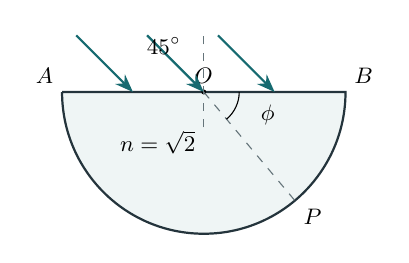
\begin{tikzpicture}[scale=.9,transform shape]
\fill[accent!7] (-2,0) arc(180:360:2)--cycle;\draw[object] (-2,0)--(2,0) arc(0:-180:2);\fill (0.00000,0.00000) circle(.035);\node[above] at (0.00000,0.00000) {$O$};\node[above left] at (-2.00000,0.00000) {$A$};\node[above right] at (2.00000,0.00000) {$B$};\draw[motion] (-1.80000,0.80000)--(-1.00000,0.00000);\draw[motion] (-0.80000,0.80000)--(0.00000,0.00000);\draw[motion] (0.20000,0.80000)--(1.00000,0.00000);\draw[guide] (0.00000,-0.50000)--(0.00000,0.90000);\node[left] at (-0.20000,0.65000) {$45^\circ$};\draw[guide] (0.00000,0.00000)--(1.28558,-1.53209);\node[below right] at (1.28558,-1.53209) {$P$};\draw[thin] (.5,0) arc(0:-50:.5);\node[right] at (0.67973,-0.31696) {$\phi$};\node[above] at (-0.65000,-1.00000) {$n=\sqrt2$};
\end{tikzpicture}
\figcaption{图光1.1\quad 平直面入射及下半圆的位置角}
\end{minipage}\end{center}

\Needspace{8\baselineskip}

\pdfbookmark[3]{题型定位}{q1-h0}

\subsection*{题型定位}

平直面折射后用边缘光线找首次受照弧，再以圆弧半径为法线求临界透射位置。用等腰三角形与坐标反延两条方法交叉核对，并明确从左右两端量角的转换；透光张角、入口束宽和透射功率是三个不同量。

\Needspace{8\baselineskip}

\pdfbookmark[3]{知识点}{q1-h1}

\subsection*{知识点}

\begin{itemize}
\item 平面入口$r=30^\circ$给所有内部光线同一方向$-60^\circ$，第二次圆弧接触必须改用局部半径法线。
\item 边缘AD与两条半径构成等腰三角形，两个底角各60度，圆心角60度要换成从右侧起算的位置角120度。
\item $P=E+\ell\vect d$同时确定入口与正向传播距离；正根才对应首次圆弧接触，不能只看无限直线与圆相交。
\item 受照弧上，朝向曲面的传播方向与外法线夹角不超过 $90^\circ$。入射角取这两个方向的夹角。
\item 玻璃向空气的临界角为45度，两临界位置15度与105度都受照，方可构成完整透光弧。
\item 切向临界点没有有限法向透射能流；改用另一端量角须反转上下界，不能只把数字逐个相减而不排序。
\end{itemize}

\Needspace{8\baselineskip}

\pdfbookmark[3]{物理图像}{q1-h2}

\subsection*{物理图像}

A图分清入口的竖直法线、内部平行方向和左端边缘AD，D限定受照弧。B图另画两临界半径与内部射线，C1、C2分别给右侧15度和105度，H处半径与内部光线同向而正入射；棕色箭头是临界切向极限。C图以实线表示真正受照范围，临界水平线切出蓝带，灰区与全反射区应区别解释。

\Needspace{8\baselineskip}

\pdfbookmark[3]{解题入口}{q1-h3}

\subsection*{解题入口}

先把位置角起算端写在图旁，再只处理入口。得内部方向后，从A求边缘点D，并用反延入口$x_0$检验受照域；这一步不需要临界角。之后才画OP法线，把方向差与45度比较，求两临界点、取受照交集并处理端点。最后换成左侧角验证同一弧段。

\Needspace{8\baselineskip}

\Needspace{18\baselineskip}
\pdfbookmark[3]{标准解法}{q1-h4}

\subsection*{标准解法}


取图光1.1中的圆心$O$为原点，平直表面为$x$轴，玻璃位于下半平面。入射光向右下方传播。设光线进入玻璃后的折射角为$r$，折射定律给出
\[
\sin45^\circ=\sqrt2\sin r,\qquad r=30^\circ.
\]
因此玻璃中的光线均沿与$x$轴成$-60^\circ$的方向传播。解图光1.1A先标出平面入口的折射角和左边缘光线AD；随后在B图的圆弧点重新画半径法线，不能继续用入口的竖直法线判断透射。
\begin{center}\begin{minipage}{.98\linewidth}\centering
\begin{tikzpicture}[scale=1.12,font=\small]
\fill[accent!5](-2,0)arc(180:360:2)--cycle;
\draw[object](-2,0)--(2,0)arc(0:-180:2);
\coordinate(O)at(0,0);\coordinate(A)at(-2,0);\coordinate(B)at(2,0);
\coordinate(D)at(-1,-1.73205081);\coordinate(H)at(1,-1.73205081);
\draw[guide](0,.85)--(0,-1.05);
\draw[motion](-1.05,1.05)--(O)--(H);
\draw[motion](A)--(D);\draw[guide](O)--(D);
\draw[motion](1.63299316,0)--(1.93185165,-.51763809);
\draw[accent,line width=1.3pt](0:2.07)arc(0:-120:2.07);
\draw(0,.45)arc(90:135:.45);\node[above left]at(-.12,.58){$45^\circ$};
\draw(0,-.62)arc(-90:-60:.62);\node at(.19,-.85){$r$};
\node[above right]at(O){$O$};\node[above left]at(A){$A$};\node[above right]at(B){$B$};
\node[below left]at(D){$D:\ \phi=120^\circ$};\node[below right]at(H){$H:\ \phi=60^\circ$};
\node[align=left,anchor=west]at(3.2,-.5){入口：$r=30^\circ$\\内部平行方向$-60^\circ$\\$AO=OD=R$\\$\angle OAD=\angle ADO=60^\circ$\\$\angle AOD=60^\circ$\\受照弧：$0<\phi<120^\circ$};
\end{tikzpicture}
\figcaption{解图光1.1A\quad 入口折射与左端边缘光线AD，边缘点D限定首次受照弧}
\end{minipage}\end{center}
图A中的边缘光线由A进入后沿AD传播。因AO水平向右，AD向右下方，$\angle OAD=60^\circ$；又因$OA=OD=R$，三角形AOD为等腰三角形，故
\[
\angle ADO=60^\circ,\qquad
\angle AOD=180^\circ-2\times60^\circ=60^\circ .
\]
从右侧半径OB向下计角时，D的位置为$\phi_D=180^\circ-60^\circ=120^\circ$。圆心角 $60^\circ=\angle AOD$ 从左侧半径量起，从右侧半径量出的 $\phi_D$ 与它互补。

先判断哪些圆弧点实际受到照明。最靠左的入射点为$A=(-R,0)$，这条边缘光线与圆周再次相交于$\phi=120^\circ$处；另一端的极限光线从$B=(R,0)$进入，对应$\phi\to0^\circ$。故用从右端量起的角度表示，第一次受照弧段为
\[
0<\phi<120^\circ.
\]
可直接验证：若$P=(R\cos\phi,-R\sin\phi)$，将光线向上反延至平面，交点横坐标为
\[
x_0=R\cos\phi-\frac{R\sin\phi}{\sqrt3}.
\]
反延的计算也可逐步写出：设入口为$E=(x_0,0)$，内部光线的单位方向为$\vect d=(1/2,-\sqrt3/2)$，于是
\[
P=E+\ell\vect d,\quad
-R\sin\phi=-\ell\sqrt3/2,\quad
\ell=\frac{2R\sin\phi}{\sqrt3},\quad
R\cos\phi=x_0+\ell/2.
\]
消去$\ell$即得前面的$x_0$。若从入口直接求首次圆弧交点，方程
\[
(x_0+\ell/2)^2+3\ell^2/4=R^2
\]
有唯一正根
\[
\ell=\frac{-x_0+\sqrt{4R^2-3x_0^2}}2\quad(-R<x_0<R).
\]
从而AD确实是左端边缘界，不能把反向延长线穿过其他区域的圆弧点算入。要求$-R<x_0<R$，在下半圆内恰给出上述区间。\begin{center}\begin{minipage}{.97\linewidth}\centering
\begin{tikzpicture}[scale=1.12,font=\small]
\fill[accent!5](-2,0)arc(180:360:2)--cycle;
\draw[object](-2,0)--(2,0)arc(0:-180:2);
\coordinate(O)at(0,0);\coordinate(Cone)at(1.93185165,-.51763809);\coordinate(Ctwo)at(-.51763809,-1.93185165);
\coordinate(H)at(1,-1.73205081);
\draw[guide](O)--(2.31822198,-.62116571);\draw[guide](O)--(-.62116571,-2.31822198);
\draw[motion](1.63299316,0)--(Cone);
\draw[motion](-1.63299316,0)--(Ctwo);
\draw[motion](O)--(H)--(1.25,-2.16506351);
\draw[force](Cone)--(1.6212688,-1.67674908);
\draw[force](Ctwo)--(.6414729,-2.2424345);
\draw[accent,line width=1.5pt](-15:2.07)arc(-15:-105:2.07);
\fill(Cone)circle(.035);\fill(Ctwo)circle(.035);\fill(H)circle(.035);
\node[above]at(O){$O$};\node[above right]at(Cone){$C_1$};\node[below left]at(Ctwo){$C_2$};
\node[right]at(1.25,-1.65){$H$};
\node[align=left,anchor=west]at(3.2,-.7){两半径为圆弧外法线\\$C_1:\phi=15^\circ,\ i=45^\circ$\\$H:\phi=60^\circ,\ i=0$\\$C_2:\phi=105^\circ,\ i=45^\circ$\\棕线：两临界切向极限\\粗弧内部：首次到达即可透射};
\end{tikzpicture}
\figcaption{解图光1.1B　两临界点的入射光与半径法线，以及切向透射极限。H处正入射，粗弧只表示两临界点之间的首次透射范围。}
\end{minipage}\end{center}


圆弧外法线的方向角为$-\phi$，而光线的方向角为$-60^\circ$，于是
\[
i=|\phi-60^\circ|.
\]
玻璃射向空气的临界角为
\[
i_c=\arcsin\frac1{\sqrt2}=45^\circ.
\]
解图光1.1B 中，入口折射决定玻璃内的固定传播方向，外法线 $\vect n=(\cos\phi,-\sin\phi)$ 则随位置转动。两者的点积给出入射角：
\[
\vect d\cdot\vect n
=\tfrac12\cos\phi+\tfrac{\sqrt3}{2}\sin\phi
=\cos(\phi-60^\circ)=\cos i.
\]
在已确定的受照弧$0<\phi<120^\circ$上，$|\phi-60^\circ|<60^\circ<90^\circ$，故此处选用的入射角确为$|\phi-60^\circ|$，不是其补角。由$i_c=45^\circ$分成两支临界条件：
\[
\phi-60^\circ=-45^\circ\Rightarrow\phi_{C_1}=15^\circ,\qquad
\phi-60^\circ=+45^\circ\Rightarrow\phi_{C_2}=105^\circ.
\]
两临界点都真实受照，它们之间又没有不可达的圆弧点，才可以连成一段透射弧。

要有传播到空气中的透射光，须$i<i_c$，因而
\[
\boxed{15^\circ<\phi<105^\circ}.
\]
该区间已包含在受照弧段内，弧长所对圆心角为$90^\circ$。在两个端点，折射光沿表面切线传播，应作为临界边界；若把切向极限也计入“透出”，可将区间端点列入，但不能将它当成具有有限法向能流的透射光束。若改从左端$A$向右计角$\phi_L=180^\circ-\phi$，同一弧段写作$75^\circ<\phi_L<165^\circ$。

\begin{center}\begin{minipage}{.97\linewidth}\centering
\begin{tikzpicture}[x=.07cm,y=.045cm,font=\small]
\path[fill=accent!8](15,0)rectangle(105,72);
\path[fill=gray!12](120,0)rectangle(130,72);
\draw[axis](0,0)--(136,0)node[right]{$\phi/(^\circ)$};
\draw[axis](0,0)--(0,79)node[above]{$i/(^\circ)$};
\draw[traj](0,60)--(60,0)--(120,60);
\draw[guide](120,60)--(130,70);
\draw[warm,dashed](0,45)--(130,45);
\foreach \x in {0,15,60,105,120}{\draw(\x,0)--(\x,-2)node[below]{$\x$};}
\foreach \y in {45,60}{\draw(0,\y)--(-2,\y)node[left]{$\y$};}
\draw[guide](15,0)--(15,45);\draw[guide](105,0)--(105,45);
\draw[accent,fill=white](15,45)circle(.055cm);\draw[accent,fill=white](105,45)circle(.055cm);
\node[above]at(66,73){$i=|\phi-60^\circ|,\quad i_c=45^\circ$};
\node[align=center]at(67,-20){浅蓝带内的实线满足$i<i_c$；临界空心点不列入\\灰区不能由平直面入口首次照到，延线只作角度比较};
\end{tikzpicture}
\figcaption{解图光1.1C　受照条件与临界角条件的交集。蓝色角区中的实线低于临界水平线，灰区则不属于首次受照弧。}
\end{minipage}\end{center}

解图光1.1C把两个筛选条件放在同一横轴上：实线先限定$0<\phi<120^\circ$，再取$i<45^\circ$。左段$0<\phi<15^\circ$和右段$105^\circ<\phi<120^\circ$虽有入射光，却发生全反射；$\phi>120^\circ$则连第一次入射都没有，两者应分别说明。

还可直接按从左端量起的$\phi_L$复算临界角，避免只靠最后换算区间。图A中$\angle AOD=60^\circ$为受照边缘，所以受照范围为$60^\circ<\phi_L<180^\circ$。固定内部方向与半径法线的夹角在两临界位置取$\pm i_c$，分别给
\[
\phi_{L,c1}=180^\circ-(60^\circ+45^\circ)=75^\circ,\qquad
\phi_{L,c2}=180^\circ-(60^\circ-45^\circ)=165^\circ .
\]
它们仍位于受照范围内。由$\phi_L=180^\circ-\phi$，15度的右侧临界点对应165度的左侧角，105度对应75度，因变换反向，转换上下界时必须交换次序。

本题的90度是透光弧所张圆心角，不是单根光线的偏向角，也不是入射光在入口上所占比例。透光圆弧两端所对应的入口为
\[
x_{0,C_1}=R\sqrt{\frac23},\qquad
x_{0,C_2}=-R\sqrt{\frac23}.
\]
所以首次可透出的入口横坐标范围为$|x_0|<R\sqrt{2/3}$。这与图B中两条临界内部平行光线吻合，也给出对圆弧位置答案的独立检查。



\Needspace{8\baselineskip}

\pdfbookmark[3]{关键洞察}{q1-h5}

\subsection*{关键洞察}

受照弧和可透射弧各有不同边界。D由入射口的左边缘决定，C1、C2由局部半径与内部方向的45度夹角决定；三个点不能相互代替。正入射中心在$\phi=60^\circ$，圆弧最低点$\phi=90^\circ$的入射角仍为30度。

\Needspace{8\baselineskip}

\pdfbookmark[3]{易错点}{q1-h6}

\subsection*{易错点}

\begin{itemize}
\item 把入口30度当作所有圆弧点的入射角，或拿竖直方向当圆弧法线。
\item 将等腰三角形的60度直接报为题干位置角，漏掉起算半径的转换。
\item 只写$i<45^\circ$而不检查入口是否在AB上，误收图C灰区。
\item 用小于号求传播透射束，最后却无说明地把切向临界点算成普通出射束。
\item 变换$\phi_L=180^\circ-\phi$后不交换上下界，误判两种角度范围互相矛盾。
\item 把90度弧宽或弧长比例当作入口光束宽度比例，或把首次透射直接等同于多次反射后的全部出射。
\end{itemize}

\Needspace{8\baselineskip}

\pdfbookmark[3]{课堂讲解建议}{q1-h7}

\subsection*{课堂讲解建议}

先在题图上让学生说清位置角从哪一端起算，再沿A图只算$r$和AD的方向。要求完整写出两个相等半径、两个底角和圆心角，说明为什么60度的$\angle AOD$对应120度的位置角。随后用入口反延式及正传播距离检验边缘判断，避免把几何草图当作可达性的证明。

转到B图，让学生分别回答最低点和H处的入射角：前者30度，后者零。固定内部光线方向，逐点转动半径，求$-45^\circ$与$+45^\circ$两支，再确认这两点都落在A图受照弧中。两支临界切线的方向也应由有向折射角求出，不能靠“远离法线”一句话随意画。

最后在C图先遮住临界线，只读受照域；再放出45度水平线取交集，并明确全反射段与根本不受照段的区别。把同一两点换成左端量角，反转排序后得到75至165度。若学生已熟练，再计算入口束宽，解释其0.8165比例为何不同于弧长3/4，而不压缩前面的法线和边界论证。

\Needspace{8\baselineskip}

\Needspace{18\baselineskip}
\pdfbookmark[3]{变式训练}{q1-h8}

\subsection*{变式训练}

\begin{enumerate}
\Needspace{7\baselineskip}
\item 将入射角改为零。内部光线竖直向下，受照整个下半圆，圆弧入射角为$|\phi-90^\circ|$，故透光区为$45^\circ<\phi<135^\circ$。\par 此时入口的全部内部光线相互平行、方向角为$-90^\circ$，正入射点也移到半圆最低点。两个临界点从该点各偏45度；端点仍是切向极限，开区间与题干约定保持一致。
\begin{center}\begin{minipage}{.98\linewidth}\centering
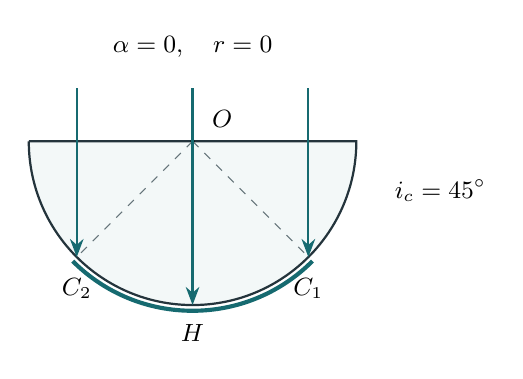
\begin{tikzpicture}[scale=1.04]\fill[accent!5](-2,0)arc(180:360:2)--cycle;\draw[object](-2,0)--(2,0)arc(0:-180:2);\fill(0,0)circle(.025);\node[above right]at(.12,.05){$O$};\coordinate(C1)at(1.41421356,-1.41421356);\draw[motion](1.41421356,0.65000000)--(1.41421356,-1.41421356);\draw[guide](0.00000000,0.00000000)--(1.41421356,-1.41421356);\node[below]at(1.41421356,-1.55421356){\(C_1\)};\coordinate(C2)at(-1.41421356,-1.41421356);\draw[motion](-1.41421356,0.65000000)--(-1.41421356,-1.41421356);\draw[guide](0.00000000,0.00000000)--(-1.41421356,-1.41421356);\node[below]at(-1.41421356,-1.55421356){\(C_2\)};\coordinate(H)at(0.00000000,-2.00000000);\draw[motion](0.00000000,0.65000000)--(0.00000000,-2.00000000);\node[below]at(0,-2.12){$H$};\draw[accent,line width=1.5pt](-45:2.07)arc(-45:-135:2.07);\node[right]at(2.35,-.6){$i_c=45^\circ$};\node[above]at(0,.9){$\alpha=0,\quad r=0$};\end{tikzpicture}
\figcaption{变图光1.1V1\quad 竖直入射时两临界半径关于最低点对称}
\end{minipage}\end{center}
\par 图V1的$H$是最低点，$OH$与竖直内部光线同向。$OC_1$、$OC_2$分别偏离$OH$四十五度，故位置角为$45^\circ$与$135^\circ$；粗弧内部满足$i<45^\circ$。两端只表示临界极限。
\Needspace{7\baselineskip}
\item 保持$45^\circ$入射，把折射率改成$n>1$。先取$r=\arcsin(\sin45^\circ/n)$，内部方向为$-(90^\circ-r)$；透射条件为$|\phi-(90^\circ-r)|<\arcsin(1/n)$，还须和边缘光线限定的区间求交。\par 边缘几何给$0<\phi<180^\circ-2r$，令$\beta=90^\circ-r$，透射区为$(\beta-i_c,\beta+i_c)\cap(0,2\beta)$，$i_c=\arcsin(1/n)$。当$n\ge\sqrt{3/2}$时$i_c\le\beta$，两临界点均在受照弧内，弧宽$2i_c$；当$1<n<\sqrt{3/2}$时$i_c>\beta$，整个首次受照弧都可透射，弧宽$2\beta$。在等号处分界与照明端点重合，用开区间表示即可。
\begin{center}\begin{minipage}{.98\linewidth}\centering
\begin{tikzpicture}[x=3.4cm,y=.045cm]\draw[axis](1,0)--(3.1,0)node[right]{$n$};\draw[axis](1,0)--(1,95)node[above]{角度/度};\draw[traj]plot coordinates{(1.02000000,78.63512303) (1.03980000,74.09625658) (1.05960000,70.69157815) (1.07940000,67.88659981) (1.09920000,65.47117777) (1.11900000,63.33619429) (1.13880000,61.41608374) (1.15860000,59.66766148) (1.17840000,58.06061963) (1.19820000,56.57267222) (1.21800000,55.18683593) (1.23780000,53.88979776) (1.25760000,52.67088035) (1.27740000,51.52135693) (1.29720000,50.43398094) (1.31700000,49.40265326) (1.33680000,48.42218063) (1.35660000,47.48809621) (1.37640000,46.59652391) (1.39620000,45.74407385) (1.41600000,44.92776068) (1.43580000,44.14493894) (1.45560000,43.39325119) (1.47540000,42.67058598) (1.49520000,41.97504347) (1.51500000,41.30490702) (1.53480000,40.65861959) (1.55460000,40.03476382) (1.57440000,39.43204537) (1.59420000,38.84927860) (1.61400000,38.28537445) (1.63380000,37.73932992) (1.65360000,37.21021902) (1.67340000,36.69718495) (1.69320000,36.19943321) (1.71300000,35.71622558) (1.73280000,35.24687486) (1.75260000,34.79074022) (1.77240000,34.34722302) (1.79220000,33.91576319) (1.81200000,33.49583593) (1.83180000,33.08694878) (1.85160000,32.68863904) (1.87140000,32.30047136) (1.89120000,31.92203564) (1.91100000,31.55294510) (1.93080000,31.19283457) (1.95060000,30.84135888) (1.97040000,30.49819145) (1.99020000,30.16302297) (2.01000000,29.83556022) (2.02980000,29.51552498) (2.04960000,29.20265300) (2.06940000,28.89669315) (2.08920000,28.59740651) (2.10900000,28.30456565) (2.12880000,28.01795387) (2.14860000,27.73736457) (2.16840000,27.46260065) (2.18820000,27.19347392) (2.20800000,26.92980459) (2.22780000,26.67142079) (2.24760000,26.41815811) (2.26740000,26.16985919) (2.28720000,25.92637332) (2.30700000,25.68755611) (2.32680000,25.45326911) (2.34660000,25.22337950) (2.36640000,24.99775983) (2.38620000,24.77628769) (2.40600000,24.55884552) (2.42580000,24.34532028) (2.44560000,24.13560331) (2.46540000,23.92959005) (2.48520000,23.72717988) (2.50500000,23.52827592) (2.52480000,23.33278484) (2.54460000,23.14061670) (2.56440000,22.95168479) (2.58420000,22.76590551) (2.60400000,22.58319819) (2.62380000,22.40348496) (2.64360000,22.22669066) (2.66340000,22.05274269) (2.68320000,21.88157090) (2.70300000,21.71310751) (2.72280000,21.54728697) (2.74260000,21.38404590) (2.76240000,21.22332298) (2.78220000,21.06505887) (2.80200000,20.90919613) (2.82180000,20.75567915) (2.84160000,20.60445404) (2.86140000,20.45546862) (2.88120000,20.30867229) (2.90100000,20.16401604) (2.92080000,20.02145231) (2.94060000,19.88093499) (2.96040000,19.74241933) (2.98020000,19.60586193) (3.00000000,19.47122063)};\draw[force]plot coordinates{(1.02000000,46.11271223) (1.03980000,47.15314176) (1.05960000,48.13839000) (1.07940000,49.07334028) (1.09920000,49.96224941) (1.11900000,50.80885374) (1.13880000,51.61645306) (1.15860000,52.38797781) (1.17840000,53.12604348) (1.19820000,53.83299515) (1.21800000,54.51094417) (1.23780000,55.16179876) (1.25760000,55.78728958) (1.27740000,56.38899133) (1.29720000,56.96834118) (1.31700000,57.52665437) (1.33680000,58.06513773) (1.35660000,58.58490130) (1.37640000,59.08696844) (1.39620000,59.57228457) (1.41600000,60.04172491) (1.43580000,60.49610120) (1.45560000,60.93616770) (1.47540000,61.36262638) (1.49520000,61.77613168) (1.51500000,62.17729458) (1.53480000,62.56668637) (1.55460000,62.94484196) (1.57440000,63.31226284) (1.59420000,63.66941977) (1.61400000,64.01675520) (1.63380000,64.35468545) (1.65360000,64.68360268) (1.67340000,65.00387672) (1.69320000,65.31585662) (1.71300000,65.61987224) (1.73280000,65.91623551) (1.75260000,66.20524173) (1.77240000,66.48717068) (1.79220000,66.76228764) (1.81200000,67.03084441) (1.83180000,67.29308011) (1.85160000,67.54922203) (1.87140000,67.79948637) (1.89120000,68.04407891) (1.91100000,68.28319569) (1.93080000,68.51702356) (1.95060000,68.74574071) (1.97040000,68.96951724) (1.99020000,69.18851557) (2.01000000,69.40289089) (2.02980000,69.61279161) (2.04960000,69.81835967) (2.06940000,70.01973094) (2.08920000,70.21703553) (2.10900000,70.41039814) (2.12880000,70.59993826) (2.14860000,70.78577054) (2.16840000,70.96800496) (2.18820000,71.14674712) (2.20800000,71.32209846) (2.22780000,71.49415642) (2.24760000,71.66301468) (2.26740000,71.82876335) (2.28720000,71.99148910) (2.30700000,72.15127538) (2.32680000,72.30820251) (2.34660000,72.46234787) (2.36640000,72.61378605) (2.38620000,72.76258890) (2.40600000,72.90882576) (2.42580000,73.05256349) (2.44560000,73.19386661) (2.46540000,73.33279742) (2.48520000,73.46941606) (2.50500000,73.60378065) (2.52480000,73.73594731) (2.54460000,73.86597033) (2.56440000,73.99390216) (2.58420000,74.11979356) (2.60400000,74.24369362) (2.62380000,74.36564985) (2.64360000,74.48570824) (2.66340000,74.60391334) (2.68320000,74.72030826) (2.70300000,74.83493481) (2.72280000,74.94783346) (2.74260000,75.05904348) (2.76240000,75.16860292) (2.78220000,75.27654870) (2.80200000,75.38291661) (2.82180000,75.48774140) (2.84160000,75.59105679) (2.86140000,75.69289550) (2.88120000,75.79328931) (2.90100000,75.89226909) (2.92080000,75.98986482) (2.94060000,76.08610564) (2.96040000,76.18101985) (2.98020000,76.27463498) (3.00000000,76.36697777)};\draw[guide](1.22474487,0.00000000)--(1.22474487,54.73561032);\fill(1.22474487,54.73561032)circle(.035cm);\node[below,align=center]at(1.22474487,-4){$\sqrt{3/2}$};\node[above]at(2.5,77){$\beta=90^\circ-r$};\node[below]at(2.4,12){$i_c=\arcsin(1/n)$};\node[above]at(2,44){$n>1$};\end{tikzpicture}
\figcaption{变图光1.1V2\quad 固定入口45度时，临界半角与受照半角的交叉}
\end{minipage}\end{center}
\par 图V2以角度为纵坐标：蓝线为$i_c$，棕线为$\beta$，两线在$n=\sqrt{3/2}$相交。交点右侧由临界角截去受照弧两端；左侧$i_c>\beta$，受照弧$(0,2\beta)$已全部落在可透射角域内。这里比较的是两个半角，弧宽还须乘二。
\Needspace{7\baselineskip}
\item 求本题透光弧长。半径为$R$时，弧段张角为$\pi/2$，故$s=\pi R/2$；不能把整个受照弧的$120^\circ$代入。\par 受照弧长为$2\pi R/3$，透光弧长为$\pi R/2$，二者比例虽为3/4，也不能直接当作均匀平行入射光的几何透出比例。入口横坐标与圆弧角并非线性关系，应由$x_0(\phi)$求对应入射束宽。
\begin{center}\begin{minipage}{.98\linewidth}\centering
\begin{tikzpicture}[scale=1.06]\fill[accent!5](-2,0)arc(180:360:2)--cycle;\draw[object](-2,0)--(2,0)arc(0:-180:2);\fill(0,0)circle(.025);\node[above right]at(.12,.05){$O$};\coordinate(C1)at(1.93185165,-0.51763809);\draw[guide](0.00000000,0.00000000)--(1.93185165,-0.51763809);\node[right]at(2.25,-.4){$C_1$};\coordinate(C2)at(-0.51763809,-1.93185165);\draw[guide](0.00000000,0.00000000)--(-0.51763809,-1.93185165);\node[below]at(-.7,-2.25){$C_2$};\draw[guide,line width=1pt](0:2.13)arc(0:-120:2.13);\draw[accent,line width=1.6pt](-15:2.03)arc(-15:-105:2.03);\draw(-15:.6)arc(-15:-105:.6);\node[below]at(.38,-.62){$90^\circ$};\node[right]at(2.4,-1){$s=\pi R/2$};\node[left]at(-1.4,-1.8){受照弧至$120^\circ$};\node[above left]at(-.2,-.6){$R$};\end{tikzpicture}
\figcaption{变图光1.1V3\quad 透光弧与首次受照弧分别计长}
\end{minipage}\end{center}
\par 图V3的蓝色粗弧从$C_1$延至$C_2$，圆心角为$105^\circ-15^\circ=90^\circ=\pi/2$。外侧虚弧延至$120^\circ$，只表示受照范围。弧长公式$s=R\Delta\phi$使用弧度，因此蓝弧长为$\pi R/2$。
\Needspace{7\baselineskip}
\item 求$\phi=90^\circ$点的折射角。$i=30^\circ$，由$\sin t=\sqrt2\sin30^\circ$得$t=45^\circ$，可把出射方向补画在图中检验折射远离法线。
\par 从法线方向$-90^\circ$向内部光传播方向转动的有向角为$+30^\circ$，折射离开法线到$+45^\circ$，所以出射方向角为$-45^\circ$。若画成向左下方或仍沿$-60^\circ$，都与折射定律不符；可在图B最低点补一条半径再作检验。
\begin{center}\begin{minipage}{.98\linewidth}\centering
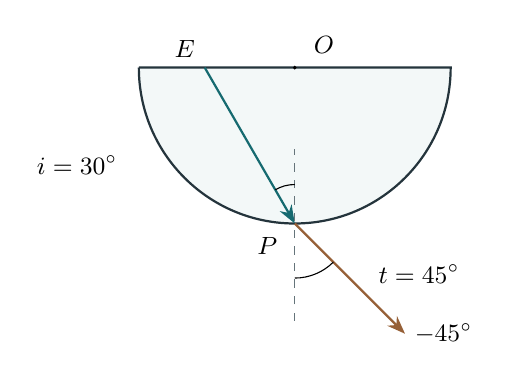
\begin{tikzpicture}[scale=.99]\fill[accent!5](-2,0)arc(180:360:2)--cycle;\draw[object](-2,0)--(2,0)arc(0:-180:2);\fill(0,0)circle(.025);\node[above right]at(.12,.05){$O$};\coordinate(E)at(-1.15470054,0.00000000);\coordinate(P)at(0.00000000,-2.00000000);\coordinate(T)at(1.41421356,-3.41421356);\draw[motion](-1.15470054,0.00000000)--(0.00000000,-2.00000000);\draw[force](0.00000000,-2.00000000)--(1.41421356,-3.41421356);\draw[guide](0,-3.25)--(0,-1.05);\draw(0,-1.5)arc(90:120:.5);\node[left]at(-2.15,-1.25){$i=30^\circ$};\draw(0,-2.7)arc(-90:-45:.7);\node[right]at(.95,-2.65){$t=45^\circ$};\node[above left]at(E){$E$};\node[below left]at(-.1,-2.05){$P$};\node[right]at(T){$-45^\circ$};\end{tikzpicture}
\figcaption{变图光1.1V4\quad 最低点的内外法线与实际出射光线}
\end{minipage}\end{center}
\par 图V4在最低点$P$画竖直法线。入射角由$PE$与向上的法线量得$30^\circ$；出射角在外部由向下的法线量得$45^\circ$。棕色射线向右下传播，方向角为$-90^\circ+45^\circ=-45^\circ$。
\Needspace{7\baselineskip}
\item 求能在首次圆弧接触时透出的入射光束宽度。将$\phi=15^\circ,105^\circ$分别代入$x_0/R=\cos\phi-\sin\phi/\sqrt3$，得$x_0/R=\pm\sqrt{2/3}$，宽度$2R\sqrt{2/3}$。若入口上入射功率密度均匀，并只统计有可透射路径而忽略反射损耗，比例为$\sqrt{2/3}\simeq0.8165$，不是圆弧长度比例3/4；要算实际功率还须按各点透射率加权。
\begin{center}\begin{minipage}{.98\linewidth}\centering
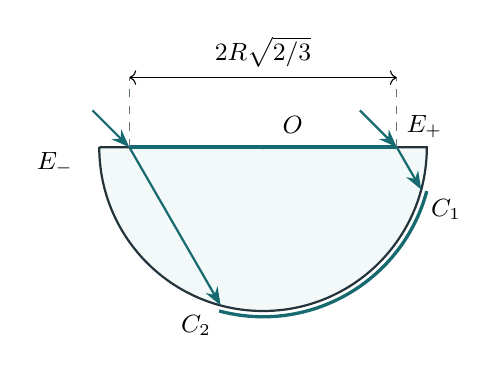
\begin{tikzpicture}[scale=1.04]\fill[accent!5](-2,0)arc(180:360:2)--cycle;\draw[object](-2,0)--(2,0)arc(0:-180:2);\fill(0,0)circle(.025);\node[above right]at(.12,.05){$O$};\coordinate(EL)at(-1.63299316,0.00000000);\coordinate(ER)at(1.63299316,0.00000000);\coordinate(C1)at(1.93185165,-0.51763809);\coordinate(C2)at(-0.51763809,-1.93185165);\draw[motion](-1.63299316,0.00000000)--(-0.51763809,-1.93185165);\draw[motion](1.63299316,0.00000000)--(1.93185165,-0.51763809);\draw[motion](-2.08299316,0.45000000)--(-1.63299316,0.00000000);\draw[motion](1.18299316,0.45000000)--(1.63299316,0.00000000);\draw[accent,line width=1.6pt](EL)--(ER);\draw[<->](-1.63299316,.85)--(1.63299316,.85)node[midway,above]{$2R\sqrt{2/3}$};\draw[guide](-1.63299316,0)--(-1.63299316,.85);\draw[guide](1.63299316,0)--(1.63299316,.85);\node[left]at(-2.2,-.2){$E_-$};\node[above right]at(ER){$E_+$};\node[below right]at(C1){$C_1$};\node[below left]at(C2){$C_2$};\draw[accent,line width=1.2pt](-15:2.07)arc(-15:-105:2.07);\end{tikzpicture}
\figcaption{变图光1.1V5\quad 两条临界入射线截出的入口束宽}
\end{minipage}\end{center}
\par 图V5把两临界点沿内部方向反延至$E_-$、$E_+$。平直面上的蓝段才是均匀入射功率对应的入口范围，其长度为$2R\sqrt{2/3}$；圆弧上的蓝线用于定位两条边缘射线。计算几何比例时，将入口蓝段除以整个入口宽$2R$。
\Needspace{7\baselineskip}
\item 把平面入射角改为任意$0\le\alpha<90^\circ$，怎样保持同一解题顺序？先由$r=\arcsin(\sin\alpha/n)$定内部方向，令$\beta=90^\circ-r$；边缘等腰三角形给受照弧$(0,2\beta)$，半径法线给$i=|\phi-\beta|$，最后取$(\beta-i_c,\beta+i_c)\cap(0,2\beta)$。张角为$2\min(\beta,i_c)$，说明“先照到、再透出”的交集步骤比记15度和105度更可迁移。
\begin{center}\begin{minipage}{.98\linewidth}\centering
\begin{tikzpicture}[x=.073cm,y=.042cm]\draw[axis](0,0)--(95,0)node[right]{$\alpha/^\circ$};\draw[axis](0,0)--(0,96)node[above]{半角/度};\draw[traj]plot coordinates{(0.00000000,90.00000000) (1.00000000,89.09091710) (2.00000000,88.18188229) (3.00000000,87.27294374) (4.00000000,86.36414982) (5.00000000,85.45554919) (6.00000000,84.54719088) (7.00000000,83.63912440) (8.00000000,82.73139985) (9.00000000,81.82406799) (10.00000000,80.91718040) (11.00000000,80.01078951) (12.00000000,79.10494878) (13.00000000,78.19971280) (14.00000000,77.29513738) (15.00000000,76.39127969) (16.00000000,75.48819842) (17.00000000,74.58595386) (18.00000000,73.68460809) (19.00000000,72.78422512) (20.00000000,71.88487102) (21.00000000,70.98661411) (22.00000000,70.08952515) (23.00000000,69.19367750) (24.00000000,68.29914732) (25.00000000,67.40601380) (26.00000000,66.51435937) (27.00000000,65.62426993) (28.00000000,64.73583511) (29.00000000,63.84914856) (30.00000000,62.96430821) (31.00000000,62.08141659) (32.00000000,61.20058115) (33.00000000,60.32191466) (34.00000000,59.44553551) (35.00000000,58.57156820) (36.00000000,57.70014371) (37.00000000,56.83140000) (38.00000000,55.96548253) (39.00000000,55.10254475) (40.00000000,54.24274874) (41.00000000,53.38626578) (42.00000000,52.53327706) (43.00000000,51.68397440) (44.00000000,50.83856098) (45.00000000,49.99725224) (46.00000000,49.16027673) (47.00000000,48.32787708) (48.00000000,47.50031105) (49.00000000,46.67785262) (50.00000000,45.86079316) (51.00000000,45.04944271) (52.00000000,44.24413136) (53.00000000,43.44521062) (54.00000000,42.65305501) (55.00000000,41.86806366) (56.00000000,41.09066200) (57.00000000,40.32130359) (58.00000000,39.56047196) (59.00000000,38.80868258) (60.00000000,38.06648491) (61.00000000,37.33446438) (62.00000000,36.61324454) (63.00000000,35.90348910) (64.00000000,35.20590393) (65.00000000,34.52123906) (66.00000000,33.85029036) (67.00000000,33.19390115) (68.00000000,32.55296342) (69.00000000,31.92841862) (70.00000000,31.32125793) (71.00000000,30.73252192) (72.00000000,30.16329931) (73.00000000,29.61472476) (74.00000000,29.08797557) (75.00000000,28.58426701) (76.00000000,28.10484617) (77.00000000,27.65098421) (78.00000000,27.22396681) (79.00000000,26.82508284) (80.00000000,26.45561129) (81.00000000,26.11680635) (82.00000000,25.80988113) (83.00000000,25.53599000) (84.00000000,25.29621034) (85.00000000,25.09152386) (86.00000000,24.92279840) (87.00000000,24.79077086) (88.00000000,24.69603188) (89.00000000,24.63901305)};\draw[force](0,65.38002267)--(89,65.38002267);\draw[guide](27.27472868,0)--(27.27472868,65.38002267);\fill(27.27472868,65.38002267)circle(.035cm);\node[below]at(27.274,0){$\alpha_*$};\node[above]at(60,67){$i_c$};\node[below]at(70,18){$\beta(\alpha)$};\node[above left]at(90,88){$n=1.10$例};\end{tikzpicture}
\figcaption{变图光1.1V6\quad 任意入口角时先比较临界半角与受照半角}
\end{minipage}\end{center}
\par 图V6取$n=1.10$作可核算的例子：$i_c$固定，$\beta(\alpha)=90^\circ-r$随$\alpha$增大而减小。交点满足$\sin\alpha_*=\sqrt{n^2-1}$，本例$\alpha_*\approx27.27^\circ$。交点左侧弧宽为$2i_c$，右侧为$2\beta$；这正是取两个角域交集的结果。
\Needspace{7\baselineskip}
\item 写本题圆弧处的有向出射方向，并核对临界点和正入射点。取方向角从$x$正轴逆时针为正，内部相对外法线的有向角为$\phi-60^\circ$，故$\vartheta_{\rm out}=-\phi+\arcsin[\sqrt2\sin(\phi-60^\circ)]$。图B在H处$\phi=60^\circ$给$-60^\circ$，两临界极限分别给$-105^\circ$与$-15^\circ$，都沿相应圆周切线；根号或反三角函数的实值条件正好又是$i\le i_c$。
\begin{center}\begin{minipage}{.98\linewidth}\centering
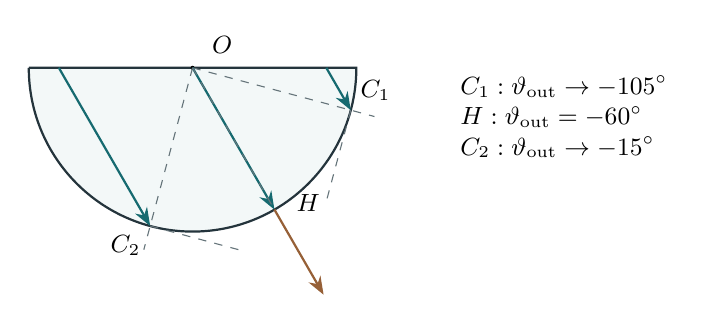
\begin{tikzpicture}[scale=1.04]\fill[accent!5](-2,0)arc(180:360:2)--cycle;\draw[object](-2,0)--(2,0)arc(0:-180:2);\fill(0,0)circle(.025);\node[above right]at(.12,.05){$O$};\coordinate(C1)at(1.93185165,-0.51763809);\coordinate(TC1)at(1.62126880,-1.67674908);\draw[motion](1.63299316,0.00000000)--(1.93185165,-0.51763809);\draw[guide](0.00000000,0.00000000)--(2.22162940,-0.59528380);\draw[guide](1.93185165,-0.51763809)--(1.62126880,-1.67674908);\node[above right]at(C1){$C_1$};\coordinate(H)at(1.00000000,-1.73205081);\coordinate(TH)at(1.60000000,-2.77128129);\draw[motion](0.00000000,0.00000000)--(1.00000000,-1.73205081);\draw[guide](0.00000000,0.00000000)--(1.15000000,-1.99185843);\draw[force](1.00000000,-1.73205081)--(1.60000000,-2.77128129);\node[right]at(1.15,-1.65){$H$};\coordinate(C2)at(-0.51763809,-1.93185165);\coordinate(TC2)at(0.64147290,-2.24243451);\draw[motion](-1.63299316,0.00000000)--(-0.51763809,-1.93185165);\draw[guide](0.00000000,0.00000000)--(-0.59528380,-2.22162940);\draw[guide](-0.51763809,-1.93185165)--(0.64147290,-2.24243451);\node[below left]at(C2){$C_2$};\node[align=left,anchor=west]at(3.15,-.6){$C_1:\vartheta_{\rm out}\to-105^\circ$\\$H:\vartheta_{\rm out}=-60^\circ$\\$C_2:\vartheta_{\rm out}\to-15^\circ$};\end{tikzpicture}
\figcaption{变图光1.1V7\quad 三处有向出射方向及临界切线极限}
\end{minipage}\end{center}
\par 图V7的$H$处射线沿半径继续传播。$C_1$、$C_2$处外部虚线分别沿方向角$-105^\circ$、$-15^\circ$，与对应半径垂直；它们表示临界切向极限。因有向角保留正负号，同一个反三角函数式能同时检验左右两端。
\Needspace{7\baselineskip}
\item 若追踪首次全反射后的后续光线，是否仍能只用图C的蓝带？不能。蓝带只统计题干限定的首次圆弧接触；全反射会改变内部方向，后续可能撞到平面或圆弧的其他点，每次都需重新确定交点和法线，再用反射或折射定律。无论后续怎样，不能反过来把未首次照到的灰区点加入第一步受照范围，这正是题干写明“第一次到达”的作用。
\begin{center}\begin{minipage}{.98\linewidth}\centering
\begin{tikzpicture}[scale=1.04]\fill[accent!5](-2,0)arc(180:360:2)--cycle;\draw[object](-2,0)--(2,0)arc(0:-180:2);\fill(0,0)circle(.025);\node[above right]at(.12,.05){$O$};\draw[accent,line width=1.1pt](0:2.07)arc(0:-120:2.07);\coordinate(E)at(1.89175061,0.00000000);\coordinate(P)at(1.99238940,-0.17431149);\coordinate(Q)at(0.51763809,-1.93185165);\coordinate(F)at(-1.63830409,-1.14715287);\coordinate(X)at(-1.63830409,0.00000000);\draw[motion](1.41175061,0.48000000)--(1.89175061,0.00000000);\draw[motion](1.89175061,0.00000000)--(1.99238940,-0.17431149);\draw[motion](1.99238940,-0.17431149)--(0.51763809,-1.93185165);\draw[motion](0.51763809,-1.93185165)--(-1.63830409,-1.14715287);\draw[motion](-1.63830409,-1.14715287)--(-1.63830409,0.00000000);\draw[force](-1.63830409,0.00000000)--(-1.63830409,0.90000000);\draw[guide](0.00000000,0.00000000)--(1.99238940,-0.17431149);\draw[guide](0.00000000,0.00000000)--(0.51763809,-1.93185165);\draw[guide](0.00000000,0.00000000)--(-1.63830409,-1.14715287);\node[right]at(P){$P:5^\circ$};\node[below right]at(Q){$Q:75^\circ$};\node[below left]at(F){$F:145^\circ$};\node[above left]at(X){$X$};\node[above right]at(E){$E$};\node[align=left,anchor=west]at(2.8,-.9){$P,Q,F$处$i=55^\circ$\\三次全反射后在$X$正入射透出};\end{tikzpicture}
\figcaption{变图光1.1V8\quad 一次首次全反射后的实际多段光路}
\end{minipage}\end{center}
\par 图V8选首次圆弧点$P$的位置角为$5^\circ$，故$i=55^\circ>i_c$。按各点半径法线反射，光线依次到$Q(75^\circ)$、$F(145^\circ)$，三处入射角同为$55^\circ$，随后竖直到达平面点$X$并正入射透出。$F$在首次受照弧之外，却能被后续光线照到；这不会改变首次受照域。
\end{enumerate}

\Needspace{13\baselineskip}

\pdfbookmark[2]{第 2 题 充液玻璃管的表观壁厚}{q2}

\section*{第 2 题\quad 充液玻璃管的表观壁厚}\label{q:2}

内半径$r$、外半径$R$的圆柱玻璃管，玻璃折射率为$n_1>1$，管内充满折射率$n_2\ge1$的发光液体。观察者在空气中从侧面远处观察。求管壁的表观厚度恰好消失时$r$与$R$应满足的条件，并讨论$n_2<n_1$和$n_2\ge n_1$两种情形。

\begin{center}\begin{minipage}{.98\linewidth}\centering
\begin{tikzpicture}[scale=.9,transform shape]
\draw[object] (0.00000,0.00000) circle(2.00000);\draw[object] (0.00000,0.00000) circle(1.50000);\draw[<->,thin,color=muted] (0.00000,0.00000)--(2.00000,0.00000);\node[below] at (1.00000,0.00000) {$R$};\draw[<->,thin,color=muted] (0.00000,0.00000)--(-1.14907,0.96418);\node[above] at (-0.57453,0.48209) {$r$};\node[above] at (-0.15000,1.05000) {$n_2$};\node[above] at (1.65000,0.60000) {$n_1$};\node[above] at (2.70000,-0.20000) {空气};\node[below] at (0.00000,-2.50000) {远处观察};
\end{tikzpicture}
\figcaption{图光1.2\quad 同心玻璃管及发光液体}
\end{minipage}\end{center}

\Needspace{8\baselineskip}

\pdfbookmark[3]{题型定位}{q2-h0}

\subsection*{题型定位}

从远处固定观察方向倒推外缘切向光线，分别核查玻璃直线能碰到内圆、液体折射能供给该方向。用三角形正弦定理展开两分支，再以同心界面的b不变量求完整表观半径，区分壁厚是否消失、每侧几何壁厚与边缘亮度。

\Needspace{8\baselineskip}

\pdfbookmark[3]{知识点}{q2-h1}

\subsection*{知识点}

\begin{itemize}
\item 观察方向固定时，外圆投影边缘M的法线OM与出射光MN垂直，外界空气给$n_1\sin i_c=1$。
\item P是液体进入玻璃的界面点，真正液体发光点可在更内部的S；三角形OPM在P处的内角是$\pi-\alpha$。
\item 玻璃直线可达内圆给$R\le n_1r$，液体中实入射角给$R\le n_2r$，两道限制都需说明。
\item 低折射率液体使$\alpha_{\max}=\arcsin(n_2/n_1)$；高折射率液体的许可角趋其临界角后，玻璃$\alpha$才趋90度。
\item b等于折射率乘以光线到圆心垂距，量纲为长度，在同心径向折射前后不变。
\item 几何表观半径$a=\min(R,n_1r,n_2r)$，每侧壁厚$w=R-a$；等号是掠射轮廓极限，不能给出边缘光强结论。
\end{itemize}

\Needspace{8\baselineskip}

\pdfbookmark[3]{物理图像}{q2-h2}

\subsection*{物理图像}

A图用一组满足条件的实际数值画S到P到M再到N的路径，OP与OM分别是局部法线。图中特意把液体发光点S和内界面P分开，避免把玻璃段误当液体段。B图比较同一材料下两种半径比的发光投影范围，灰端带是仍无直达液体光路的位置。C图把两分支接成一条条件边界，液体折射率超过玻璃后，限制不再随液体参数继续放宽。

\Needspace{8\baselineskip}

\pdfbookmark[3]{解题入口}{q2-h3}

\subsection*{解题入口}

先把平行观察方向画在外圆最左侧，再反推所需玻璃临界方向。对三角形标清r、R、$i_c$与$\pi-\alpha$，得到所需$\sin\alpha$；先问它能否小于1，再问液体角j能否为实数。比较两上限后再合并最小值，最后用b的不变量说明充分性和整条轮廓。

\Needspace{8\baselineskip}

\Needspace{18\baselineskip}
\pdfbookmark[3]{标准解法}{q2-h4}

\subsection*{标准解法}


图光1.2中管轴垂直纸面。远处观察对应近乎平行的出射光；要使发光液体的轮廓扩展到管的最外边缘，边缘$M$处必须存在沿切线$MN$出射的极限光线。解图光1.2A中S是液体内的发光点，P是光进入玻璃的内界面点，PM才是玻璃内的直线光段；P不能与液体深处的发光位置混淆。
\begin{center}\begin{minipage}{.98\linewidth}\centering
\begin{tikzpicture}[scale=1.05,font=\small]
\draw[object](0,0)circle(2);\draw[object](0,0)circle(1.6);
\coordinate(O)at(0,0);\coordinate(M)at(-2,0);\coordinate(P)at(-1.54810653,.40418581);\coordinate(S)at(-1.31920865,.79162065);
\draw[guide](O)--(-2.35,0);\draw[guide](O)--(-1.93513316,.50523226);
\draw[motion](S)--(P)--(M)--(-2,-2.7);
\fill(P)circle(.035);\fill(M)circle(.035);\fill(S)circle(.035);\fill(O)circle(.025);
\node[right]at(O){$O$};\node[above left]at(P){$P$};\node[above right]at(S){$S$};
\node[left]at(M){$M$};\node[below]at(-2,-2.7){$N$};
\draw ($(P)+(165.367625:.28)$)arc(165.367625:221.810315:.28);
\node[left]at(-2.03,.36){$\alpha$};
\draw ($(P)+(-14.632375:.25)$)arc(-14.632375:59.425256:.25);
\node at(-1.17,.61){$j$};
\draw(-1.55,0)arc(0:41.810315:.45);
\node[below]at(-1.32,.08){$i_c$};
\node at(.45,.75){液体$n_2$};\node at(1.72,.65){$n_1$};
\node[align=left,anchor=west]at(3,-.55){S为液内发光点，P在内界面\\MN为外缘切向出射极限\\半径OM、OP分别是两处法线\\图取$R=2,\ r=1.6$\\$n_1=1.5,\ n_2=1.3$\\$i_c=41.81^\circ,\ \alpha=56.44^\circ$\\液体入射角$j=74.06^\circ$};
\end{tikzpicture}
\figcaption{解图光1.2A\quad 边缘切向光线反推内界面的可供方向}
\end{minipage}\end{center}
设$PM$与外表面法线$OM$的夹角为$i_c$，与内表面法线$OP$的锐角为$\alpha$。由$M$处切向出射条件，
\[
n_1\sin i_c=1,\qquad \sin i_c=\frac1{n_1}.
\]
这里$\alpha$是PM与OP延长方向的锐角，三角形在P处的内角实际为$\pi-\alpha$，不是$\alpha$；因此完整正弦定理写为
\[
\frac r{\sin i_c}=\frac R{\sin(\pi-\alpha)}
=\frac R{\sin\alpha}.
\]
M处之所以必须用切向极限，是因为选定观察方向后，外圆投影最左点的半径OM正好与出射方向MN垂直。内界面的位置P再由这一外缘光线反推，不能任取一条近轴光线代表边缘。

在三角形$OPM$中，用正弦定理或光线相对圆心的垂距相等可得
\[
r\sin\alpha=R\sin i_c,\qquad
\sin\alpha=\frac{R}{n_1r}.
\]
所得角度确定了玻璃内的方向，还要检查液体折射出的光能否具有这个方向。若液体内的入射角为$j$，内界面满足
\[
n_2\sin j=n_1\sin\alpha.
\]
要有这样的PM，首先必须$\sin\alpha\le1$，即玻璃内的这条直线确实能交到半径r的内圆；其次还须能找到实的液体入射角j。把外缘条件代入内界面折射式，立即得到
\[
\sin j=\frac{n_1}{n_2}\sin\alpha
=\frac R{n_2r}.
\]
所以几何可达与液体可供方向分别要求$R\le n_1r$和$R\le n_2r$。下面按$n_2$与$n_1$的相对大小展开这两个限制，不能只保留较熟悉的玻璃向空气临界角。

当$n_2<n_1$时，液体射入玻璃的折射角最多为
\[
\alpha_{\max}=\arcsin(n_2/n_1).
\]
所需$\alpha$不应大于它，因此
\[
\frac{R}{n_1r}\le\frac{n_2}{n_1},\qquad
\boxed{\frac Rr\le n_2\quad(n_2<n_1)}.
\]
在这一分支，$j\to90^\circ$时内界面折射定律为$n_2\sin90^\circ=n_1\sin\alpha_{\max}$。由于$n_2/n_1<1$，所需$\alpha$的上限已经比几何90度更严格，故$n_2$控制结果；不能用“玻璃内可画出PM”代替这一供光条件。

当$n_2\ge n_1$时，玻璃中的折射方向可以逼近$\alpha=90^\circ$，故只需
\[
\frac{R}{n_1r}\le1,\qquad
\boxed{\frac Rr\le n_1\quad(n_2\ge n_1)}.
\]
当$n_2>n_1$时，液体一侧的透射角域截止于$j_c=\arcsin(n_1/n_2)$。在$j<j_c$的范围内增大$j$，玻璃中的$\alpha$随之增大；$j\to j_c$时，$\alpha\to90^\circ$。越过$j_c$后，光在液体与玻璃的界面发生全反射。若$n_2=n_1$，光线直穿内界面，入射线趋近内圆切线时也得到同一上限。

合写为
\[
\boxed{1<\frac Rr\le \min(n_1,n_2)}.
\]
该条件描述发光区轮廓能覆盖整个外径的几何极限。等号对应某一界面上的掠射极限；讨论实际观察的亮度时，不能由“轮廓达到外缘”推断边缘亮度与中央相同。若$R/r$大于上述上限，靠近外缘存在无法从液体直接到达观察方向的光线，仍能分辨管壁。


上述条件也充分。若$R\le\min(n_1,n_2)r$，从M沿玻璃内临界方向向后追踪，直线到圆心的垂距为$h=R\sin i_c=R/n_1\le r$，所以可到达内圆；在最近的内界面交点P处再取$j=\arcsin[R/(n_2r)]$，即可反推一条液体中的入射光线。严格不等号给有限传播的可透射路径，等号作为界面掠射或相切的轮廓闭包。

为了确认不只最外一点可到，还可求整个表观发光半径。对任意同心界面上的光线，令
\[
b=n\,s\sin\eta ,
\]
其中s是该界面半径，$\eta$是光线与当地半径法线的夹角。直线段到圆心的垂距是$s\sin\eta$，同一介质内它不变；界面上又有$n\sin\eta$连续，故同一条光路的b在两次折射前后不变。b具有长度量纲，不是无量纲折射率本身。

远处沿竖直方向观察，在空气中$b=|x_{\rm obs}|$。若要反推到液体，必须同时满足
\[
b\le R,\qquad b\le n_1r,\qquad b\le n_2r .
\]
第一式保证外圆有交点，第二式保证玻璃内反向光线能碰到内圆，第三式保证液体中存在实入射角。由此得到表观发光半径a和每侧表观壁厚w：
\[
a=\min\{R,n_1r,n_2r\},\qquad
w=R-a=\max\{0,R-\min(n_1,n_2)r\}.
\]
当$a=R$时整个外径均可由发光液体的光路覆盖，就恢复前面的壁厚消失条件。所有比极限b更小的位置也有可供路径，这补足了只检验最外缘时的存在性说明。
\begin{center}\begin{minipage}{.97\linewidth}\centering
\begin{tikzpicture}[x=4cm,y=1cm,font=\small]
\node[align=center]at(0,1.7){固定$n_1=1.5,\ n_2=1.3$，观察平面位置$x_{\rm obs}/R$\\色带只示光路存在范围，不给亮度分布};
\path[fill=gray!30](-1,.8)rectangle(1,1.08);
\path[fill=accent!40](-.91,.8)rectangle(.91,1.08);
\draw[object](-1,.8)rectangle(1,1.08);
\foreach \x/\v in {-1/-1,0/0,1/1}{\draw(\x,.8)--(\x,.7)node[below]{$\v$};}
\node[align=left,anchor=west]at(1.2,.95){$r/R=0.70$\\$a/R=0.91$\\每侧仍见$0.09R$};
\path[fill=gray!30](-1,-1)rectangle(1,-.72);
\path[fill=accent!40](-1,-1)rectangle(1,-.72);
\draw[object](-1,-1)rectangle(1,-.72);
\foreach \x/\v in {-1/-1,0/0,1/1}{\draw(\x,-1)--(\x,-1.1)node[below]{$\v$};}
\node[align=left,anchor=west]at(1.2,-.85){$r/R=0.80$\\$a/R=1$\\发光轮廓覆盖整个外径};
\end{tikzpicture}
\figcaption{解图光1.2B　同一玻璃和液体下，两种内外半径比的表观轮廓。灰色端带标出液体直达光线到不了的壁区，色带标出轮廓的可见范围。}
\end{minipage}\end{center}

解图光1.2B固定$n_1=1.5,n_2=1.3$。上图$r/R=0.70$时，$a/R=\min(1,1.05,0.91)=0.91$，每侧仍有$0.09R$表观壁区；下图$r/R=0.80$时，$a/R=\min(1,1.20,1.04)=1$，发光轮廓延至外缘。两个例子都不是把物理壁厚$R-r$直接缩放成表观厚度，控制量是折射与几何可达性共同允许的最大b。
\begin{center}\begin{minipage}{.97\linewidth}\centering
\begin{tikzpicture}[x=12cm,y=3cm,font=\small]
\path[fill=accent!12](.66666667,1)--(.66666667,.5)--plot[domain=.66666667:1,samples=90](\x,{1/\x-1})--(1,1)--cycle;
\draw[axis](.5,0)--(1.06,0)node[right]{$\rho=r/R$};
\draw[axis](.5,0)--(.5,1.13)node[above]{$n_2$};
\foreach \x/\v in {.5/.5,.66666667/{2/3},.8/.8,1/1}{\draw(\x,0)--(\x,-.025)node[below]{$\v$};}
\foreach \y/\v in {0/1,.5/1.5,1/2}{\draw(.5,\y)--(.49,\y)node[left]{$\v$};}
\draw[guide](.5,.5)--(1,.5);
\draw[traj](.66666667,1)--(.66666667,.5);
\draw[traj,domain=.66666667:1,samples=90]plot(\x,{1/\x-1});
\fill[warm](.7,.3)circle(.045cm);\node[below left]at(.7,.3){B上};
\fill[accent](.8,.3)circle(.045cm);\node[above right]at(.8,.3){B下};
\node[above]at(.8,1.13){图取$n_1=1.5$};
\node[align=left,anchor=west]at(1.18,.6){浅蓝：几何轮廓覆盖外径\\$n_2<1.5:\ \rho\ge1/n_2$\\$n_2\ge1.5:\ \rho\ge2/3$\\两段边界在$n_2=n_1$连接\\真实管壁另需$\rho<1$};
\end{tikzpicture}
\figcaption{解图光1.2C　固定玻璃折射率1.5的条件图。浅蓝区域满足两次折射的方向存在性，B中的两个例子位于分界两侧。}
\end{minipage}\end{center}

在解图光1.2C中，$\rho=r/R$。液体折射率较低时边界为$\rho=1/n_2$；提高到$n_2=n_1$后，边界固定为$\rho=1/n_1$，再提高$n_2$也不能让玻璃内的直线穿过它本来碰不到的内圆。若$n_2=1$，条件要求$\rho\ge1$，与非零厚度的$\rho<1$冲突；因此不能靠同折射率为空气的发光介质消去一个有有限厚度的管壁轮廓。

本题只判几何发光轮廓。界面的透射率、液体吸收和发光分布会改变亮度，但不允许把违反上述方向存在性的位置宣称为液体的直达出射光；在掠射边界也不能从a达到R推断有与中央相同的边缘强度。



\Needspace{8\baselineskip}

\pdfbookmark[3]{关键洞察}{q2-h5}

\subsection*{关键洞察}

玻璃内可画出的极限方向未必能从液体折射得到；液体折射率很高也不能让玻璃内不碰内圆的直线接上发光区域。前一限制在$n_2<n_1$时更严格，后一限制在$n_2\ge n_1$时控制，二者在相等处连续连接。

\Needspace{8\baselineskip}

\pdfbookmark[3]{易错点}{q2-h6}

\subsection*{易错点}

\begin{itemize}
\item 默认液体能供给任何玻璃方向，只检查$R/r\le n_1$而漏掉$n_2$。
\item 用三角形在P处的锐角$\alpha$作图，却没有说明真正内角是$\pi-\alpha$；或把P画成液体深处的发光点。
\item 高折射率液体一侧把所有j都算作可透射，而没有限制到$j_c=\arcsin(n_1/n_2)$。
\item 用近轴像大小或一根中心亮光代替整个外缘的光路存在性。
\item 把b当无量纲数，或把外介质折射率改变后仍写$b=|x_{\rm obs}|$。
\item 从$a=R$推断边缘亮度与中心相同，或从轮廓消失推断物理壁厚等于零。
\end{itemize}

\Needspace{8\baselineskip}

\pdfbookmark[3]{课堂讲解建议}{q2-h7}

\subsection*{课堂讲解建议}

先让学生在A图沿S、P、M、N逐段指出介质，明确P是界面点。只看固定观察方向，要求解释为何M处外角90度，再完整写出三角形内角和正弦定理，不急于报最小值。

把所需$\sin\alpha$写在左边，右边依次检查几何上限1和液体折射上限$n_2/n_1$。分别让两组学生讨论低折射率与高折射率液体，后一组需指出j的许可范围，不能说液体任意角都能进入玻璃。最后在$n_2=n_1$处核对两组答案相接。

沿B图比较同材料两种半径比，算a与w，再用C图解释为何继续提高液体折射率会出现上限。追问$n_2=1$和固定$r/R=0.80$两种情形，要求先核查玻璃、再核查液体。若有余力，让学生从垂距与Snell证明b守恒，用所有$b<R$的反向构造补足充分性；亮度问题应回到透射率和发光分布，不能从几何轮廓一句带过。

\Needspace{8\baselineskip}

\Needspace{18\baselineskip}
\pdfbookmark[3]{变式训练}{q2-h8}

\subsection*{变式训练}

\begin{enumerate}
\Needspace{7\baselineskip}
\item 取$n_1=1.5,n_2=1.33$，求$r/R$下限。由$R/r\le1.33$得$r/R\ge0.7519$，所以管壁厚度不应超过约$0.2481R$。\par 精确下限为$1/1.33=0.7518797$，最大几何壁厚为$(1-1/1.33)R=0.2481203R$。在此下限处液体角趋90度，几何轮廓达到边缘属于极限；若需要有余量的可透射路径，应取$r/R$严格大于此值，而不能把临界等号等同于有限亮度。
\begin{center}\begin{minipage}{.98\linewidth}\centering
\begin{tikzpicture}[x=6cm,y=3.1cm]\draw[axis](0,0)--(1.1,0)node[right]{$r/R$};\draw[axis](0,0)--(0,1.15)node[above]{$a/R$};\draw[traj]plot coordinates{(0.00000000,0.00000000) (0.01000000,0.01330000) (0.02000000,0.02660000) (0.03000000,0.03990000) (0.04000000,0.05320000) (0.05000000,0.06650000) (0.06000000,0.07980000) (0.07000000,0.09310000) (0.08000000,0.10640000) (0.09000000,0.11970000) (0.10000000,0.13300000) (0.11000000,0.14630000) (0.12000000,0.15960000) (0.13000000,0.17290000) (0.14000000,0.18620000) (0.15000000,0.19950000) (0.16000000,0.21280000) (0.17000000,0.22610000) (0.18000000,0.23940000) (0.19000000,0.25270000) (0.20000000,0.26600000) (0.21000000,0.27930000) (0.22000000,0.29260000) (0.23000000,0.30590000) (0.24000000,0.31920000) (0.25000000,0.33250000) (0.26000000,0.34580000) (0.27000000,0.35910000) (0.28000000,0.37240000) (0.29000000,0.38570000) (0.30000000,0.39900000) (0.31000000,0.41230000) (0.32000000,0.42560000) (0.33000000,0.43890000) (0.34000000,0.45220000) (0.35000000,0.46550000) (0.36000000,0.47880000) (0.37000000,0.49210000) (0.38000000,0.50540000) (0.39000000,0.51870000) (0.40000000,0.53200000) (0.41000000,0.54530000) (0.42000000,0.55860000) (0.43000000,0.57190000) (0.44000000,0.58520000) (0.45000000,0.59850000) (0.46000000,0.61180000) (0.47000000,0.62510000) (0.48000000,0.63840000) (0.49000000,0.65170000) (0.50000000,0.66500000) (0.51000000,0.67830000) (0.52000000,0.69160000) (0.53000000,0.70490000) (0.54000000,0.71820000) (0.55000000,0.73150000) (0.56000000,0.74480000) (0.57000000,0.75810000) (0.58000000,0.77140000) (0.59000000,0.78470000) (0.60000000,0.79800000) (0.61000000,0.81130000) (0.62000000,0.82460000) (0.63000000,0.83790000) (0.64000000,0.85120000) (0.65000000,0.86450000) (0.66000000,0.87780000) (0.67000000,0.89110000) (0.68000000,0.90440000) (0.69000000,0.91770000) (0.70000000,0.93100000) (0.71000000,0.94430000) (0.72000000,0.95760000) (0.73000000,0.97090000) (0.74000000,0.98420000) (0.75000000,0.99750000) (0.76000000,1.00000000) (0.77000000,1.00000000) (0.78000000,1.00000000) (0.79000000,1.00000000) (0.80000000,1.00000000) (0.81000000,1.00000000) (0.82000000,1.00000000) (0.83000000,1.00000000) (0.84000000,1.00000000) (0.85000000,1.00000000) (0.86000000,1.00000000) (0.87000000,1.00000000) (0.88000000,1.00000000) (0.89000000,1.00000000) (0.90000000,1.00000000) (0.91000000,1.00000000) (0.92000000,1.00000000) (0.93000000,1.00000000) (0.94000000,1.00000000) (0.95000000,1.00000000) (0.96000000,1.00000000) (0.97000000,1.00000000) (0.98000000,1.00000000) (0.99000000,1.00000000) (1.00000000,1.00000000)};\draw[guide](0,1)--(1,1); \draw[guide](0.75187970,0)--(0.75187970,1);\fill(0.75187970,1)circle(.035cm);\node[left]at(0,1){$1$};\node[below]at(.75187970,0){$1/1.33$};\node[above]at(.4,.75){$a/R=1.33\,r/R$};\node[above]at(.88,1.02){轮廓覆盖};\end{tikzpicture}
\figcaption{变图光1.2V1\quad 液体折射率1.33时表观半径随内半径的变化}
\end{minipage}\end{center}
\par 图V1的蓝线在$r/R=1/1.33$达到$a/R=1$，之后由外圆半径截住。交点左侧仍有表观壁厚；交点本身是液体方向趋于切向的极限。需要有限角度余量时，应在交点右侧取值。
\Needspace{7\baselineskip}
\item 若$n_2=1.7,n_1=1.5$，条件为$r/R\ge2/3$。虽然液体折射率增加，限制仍由玻璃中的折射方向决定。\par 此时在$r/R=2/3$极限，玻璃方向$\alpha\to90^\circ$，液体入射角仅需$j\to\arcsin(1.5/1.7)\simeq61.93^\circ$。限制已从液体可供方向转成玻璃直线能否交内圆，继续增加$n_2$不能放宽第二道几何条件。
\begin{center}\begin{minipage}{.98\linewidth}\centering
\begin{tikzpicture}[x=15cm,y=.04cm]\draw[axis](.64,0)--(1.025,0)node[right]{$r/R$};\draw[axis](.64,0)--(.64,99)node[above]{方向角/度};\draw[traj]plot coordinates{(0.66666667,90.00000000) (0.67083333,83.61075210) (0.67500000,80.98754850) (0.67916667,78.99036781) (0.68333333,77.31961651) (0.68750000,75.85888977) (0.69166667,74.54830657) (0.69583333,73.35218637) (0.70000000,72.24720984) (0.70416667,71.21712910) (0.70833333,70.25007720) (0.71250000,69.33706735) (0.71666667,68.47109559) (0.72083333,67.64657440) (0.72500000,66.85895897) (0.72916667,66.10449181) (0.73333333,65.38002267) (0.73750000,64.68287834) (0.74166667,64.01076642) (0.74583333,63.36170269) (0.75000000,62.73395555) (0.75416667,62.12600265) (0.75833333,61.53649677) (0.76250000,60.96423849) (0.76666667,60.40815421) (0.77083333,59.86727817) (0.77500000,59.34073769) (0.77916667,58.82774092) (0.78333333,58.32756657) (0.78750000,57.83955532) (0.79166667,57.36310250) (0.79583333,56.89765185) (0.80000000,56.44269024) (0.80416667,55.99774299) (0.80833333,55.56236996) (0.81250000,55.13616205) (0.81666667,54.71873817) (0.82083333,54.30974264) (0.82500000,53.90884276) (0.82916667,53.51572685) (0.83333333,53.13010235) (0.83750000,52.75169421) (0.84166667,52.38024345) (0.84583333,52.01550583) (0.85000000,51.65725074) (0.85416667,51.30526008) (0.85833333,50.95932736) (0.86250000,50.61925685) (0.86666667,50.28486277) (0.87083333,49.95596860) (0.87500000,49.63240646) (0.87916667,49.31401649) (0.88333333,49.00064635) (0.88750000,48.69215071) (0.89166667,48.38839081) (0.89583333,48.08923405) (0.90000000,47.79455360) (0.90416667,47.50422805) (0.90833333,47.21814113) (0.91250000,46.93618135) (0.91666667,46.65824177) (0.92083333,46.38421972) (0.92500000,46.11401657) (0.92916667,45.84753753) (0.93333333,45.58469140) (0.93750000,45.32539044) (0.94166667,45.06955012) (0.94583333,44.81708902) (0.95000000,44.56792865) (0.95416667,44.32199328) (0.95833333,44.07920985) (0.96250000,43.83950780) (0.96666667,43.60281897) (0.97083333,43.36907751) (0.97500000,43.13821973) (0.97916667,42.91018402) (0.98333333,42.68491077) (0.98750000,42.46234227) (0.99166667,42.24242262) (0.99583333,42.02509766) (1.00000000,41.81031490)};\draw[force]plot coordinates{(0.66666667,61.92751306) (0.67083333,61.26736456) (0.67500000,60.62871108) (0.67916667,60.01007559) (0.68333333,59.41014404) (0.68750000,58.82774092) (0.69166667,58.26180938) (0.69583333,57.71139486) (0.70000000,57.17563163) (0.70416667,56.65373140) (0.70833333,56.14497387) (0.71250000,55.64869869) (0.71666667,55.16429855) (0.72083333,54.69121339) (0.72500000,54.22892527) (0.72916667,53.77695407) (0.73333333,53.33485362) (0.73750000,52.90220843) (0.74166667,52.47863076) (0.74583333,52.06375807) (0.75000000,51.65725074) (0.75416667,51.25879008) (0.75833333,50.86807654) (0.76250000,50.48482813) (0.76666667,50.10877898) (0.77083333,49.73967808) (0.77500000,49.37728812) (0.77916667,49.02138447) (0.78333333,48.67175422) (0.78750000,48.32819535) (0.79166667,47.99051597) (0.79583333,47.65853359) (0.80000000,47.33207451) (0.80416667,47.01097321) (0.80833333,46.69507184) (0.81250000,46.38421972) (0.81666667,46.07827289) (0.82083333,45.77709369) (0.82500000,45.48055040) (0.82916667,45.18851686) (0.83333333,44.90087216) (0.83750000,44.61750034) (0.84166667,44.33829012) (0.84583333,44.06313461) (0.85000000,43.79193111) (0.85416667,43.52458086) (0.85833333,43.26098882) (0.86250000,43.00106351) (0.86666667,42.74471683) (0.87083333,42.49186383) (0.87500000,42.24242262) (0.87916667,41.99631420) (0.88333333,41.75346231) (0.88750000,41.51379329) (0.89166667,41.27723600) (0.89583333,41.04372166) (0.90000000,40.81318376) (0.90416667,40.58555796) (0.90833333,40.36078199) (0.91250000,40.13879556) (0.91666667,39.91954028) (0.92083333,39.70295956) (0.92500000,39.48899855) (0.92916667,39.27760407) (0.93333333,39.06872453) (0.93750000,38.86230987) (0.94166667,38.65831151) (0.94583333,38.45668226) (0.95000000,38.25737630) (0.95416667,38.06034910) (0.95833333,37.86555740) (0.96250000,37.67295913) (0.96666667,37.48251337) (0.97083333,37.29418034) (0.97500000,37.10792132) (0.97916667,36.92369862) (0.98333333,36.74147557) (0.98750000,36.56121643) (0.99166667,36.38288643) (0.99583333,36.20645165) (1.00000000,36.03187907)};\draw[guide](.66666667,0)--(.66666667,90);\node[below]at(.66666667,0){$2/3$};\node[above]at(.85,57){$\alpha$（玻璃）};\node[below]at(.9,33){$j$（液体）};\node[above right]at(.7,86){$n_1=1.5,\ n_2=1.7$};\end{tikzpicture}
\figcaption{变图光1.2V2\quad 外缘极限所需的玻璃角与液体角}
\end{minipage}\end{center}
\par 图V2按外缘$b=R$作图，故$\sin\alpha=1/(1.5\,r/R)$、$\sin j=1/(1.7\,r/R)$。在$r/R=2/3$处，玻璃角$\alpha$先到$90^\circ$，液体角只有$61.93^\circ$。因此这一例子的限制来自玻璃直线能否到内圆。
\Needspace{7\baselineskip}
\item 外部改为折射率$n_e$的介质，且$n_1>n_e$。$n_1\sin i_c=n_e$，推得$R/r\le\min(n_1,n_2)/n_e$，应同时检查右端是否大于1。\par 一般表观半径为$a=\min[R,\min(n_1,n_2)r/n_e]$，因空气中$b=|x_{\rm obs}|$要改为外介质中的$b=n_e|x_{\rm obs}|$。若$\min(n_1,n_2)\le n_e$，非零壁厚无法满足；若外介质改变后$n_1\le n_e$，则不能继续把外圆的极限光线称为玻璃向外的全反射临界光线，应重新从方向可达性讨论。
\begin{center}\begin{minipage}{.98\linewidth}\centering
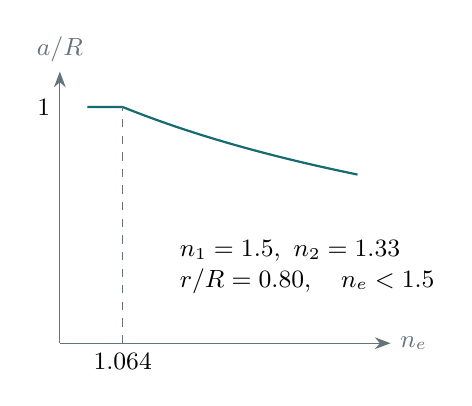
\begin{tikzpicture}[x=7cm,y=3cm]\draw[axis](.95,0)--(1.55,0)node[right]{$n_e$};\draw[axis](.95,0)--(.95,1.15)node[above]{$a/R$};\draw[traj]plot coordinates{(1.00000000,1.00000000) (1.00490000,1.00000000) (1.00980000,1.00000000) (1.01470000,1.00000000) (1.01960000,1.00000000) (1.02450000,1.00000000) (1.02940000,1.00000000) (1.03430000,1.00000000) (1.03920000,1.00000000) (1.04410000,1.00000000) (1.04900000,1.00000000) (1.05390000,1.00000000) (1.05880000,1.00000000) (1.06370000,1.00000000) (1.06860000,0.99569530) (1.07350000,0.99115044) (1.07840000,0.98664688) (1.08330000,0.98218407) (1.08820000,0.97776144) (1.09310000,0.97337846) (1.09800000,0.96903461) (1.10290000,0.96472935) (1.10780000,0.96046218) (1.11270000,0.95623259) (1.11760000,0.95204009) (1.12250000,0.94788419) (1.12740000,0.94376441) (1.13230000,0.93968030) (1.13720000,0.93563138) (1.14210000,0.93161720) (1.14700000,0.92763731) (1.15190000,0.92369129) (1.15680000,0.91977870) (1.16170000,0.91589911) (1.16660000,0.91205212) (1.17150000,0.90823730) (1.17640000,0.90445427) (1.18130000,0.90070262) (1.18620000,0.89698196) (1.19110000,0.89329192) (1.19600000,0.88963211) (1.20090000,0.88600217) (1.20580000,0.88240172) (1.21070000,0.87883043) (1.21560000,0.87528792) (1.22050000,0.87177386) (1.22540000,0.86828791) (1.23030000,0.86482972) (1.23520000,0.86139896) (1.24010000,0.85799532) (1.24500000,0.85461847) (1.24990000,0.85126810) (1.25480000,0.84794390) (1.25970000,0.84464555) (1.26460000,0.84137277) (1.26950000,0.83812525) (1.27440000,0.83490270) (1.27930000,0.83170484) (1.28420000,0.82853138) (1.28910000,0.82538205) (1.29400000,0.82225657) (1.29890000,0.81915467) (1.30380000,0.81607609) (1.30870000,0.81302055) (1.31360000,0.80998782) (1.31850000,0.80697763) (1.32340000,0.80398972) (1.32830000,0.80102387) (1.33320000,0.79807981) (1.33810000,0.79515731) (1.34300000,0.79225614) (1.34790000,0.78937607) (1.35280000,0.78651685) (1.35770000,0.78367828) (1.36260000,0.78086012) (1.36750000,0.77806216) (1.37240000,0.77528417) (1.37730000,0.77252596) (1.38220000,0.76978730) (1.38710000,0.76706798) (1.39200000,0.76436782) (1.39690000,0.76168659) (1.40180000,0.75902411) (1.40670000,0.75638018) (1.41160000,0.75375460) (1.41650000,0.75114719) (1.42140000,0.74855776) (1.42630000,0.74598612) (1.43120000,0.74343208) (1.43610000,0.74089548) (1.44100000,0.73837613) (1.44590000,0.73587385) (1.45080000,0.73338848) (1.45570000,0.73091983) (1.46060000,0.72846775) (1.46550000,0.72603207) (1.47040000,0.72361262) (1.47530000,0.72120925) (1.48020000,0.71882178) (1.48510000,0.71645007) (1.49000000,0.71409396)};\draw[guide](1.064,0)--(1.064,1);\node[below]at(1.064,0){$1.064$};\node[above right,align=left]at(1.15,.17){$n_1=1.5,\ n_2=1.33$\\$r/R=0.80,\quad n_e<1.5$};\node[left]at(.95,1){$1$};\end{tikzpicture}
\figcaption{变图光1.2V3\quad 外介质折射率改变时的表观半径}
\end{minipage}\end{center}
\par 图V3取$n_1=1.5,n_2=1.33,r/R=0.80$，蓝线为$a/R=\min(1,1.064/n_e)$。$n_e=1.064$是覆盖外径的分界；增大外介质折射率使可见液体轮廓缩小。图中只画$n_e<n_1$的区间，与玻璃向外的临界条件一致。
\Needspace{7\baselineskip}
\item 用光学动量重做。外缘切向光线的$b=n_eR$，内圆和液体分别允许$b\le n_1r$、$b\le n_2r$；两式联立即得到一般条件，避免逐角讨论时漏掉一个界面。
\par 应先证明n乘以到圆心垂距在直线段不变、在径向界面由Snell连续，再写两个内界面上限。若只把b当作一个无量纲n或省去r，就会得到量纲不一致的条件。外缘$b=n_eR$的要求是必要的，较小b的同样反向构造则说明充分性。
\begin{center}\begin{minipage}{.98\linewidth}\centering
\begin{tikzpicture}[scale=.95]\fill[muted!10](0,0)circle(2);\fill[accent!10](0,0)circle(1.60000000);\draw[object](0,0)circle(2) (0,0)circle(1.60000000);\draw[guide](0,0)--(-1.60000000,0);\draw[guide](0,0)--(0,-2);\fill(0,0)circle(.025);\node[below left]at(-.05,-.1){$O$};\node[below]at(0,-2.05){$R$};\node[above]at(-.7,0){$r$};\coordinate(P)at(0.00000000,2.00000000);\coordinate(Q)at(-0.40418581,1.54810653);\coordinate(S)at(-0.96381392,1.21747626);\draw[motion](2.80000000,2.00000000)--(0.00000000,2.00000000);\draw[motion](0.00000000,2.00000000)--(-0.40418581,1.54810653);\draw[force](-0.40418581,1.54810653)--(-0.96381392,1.21747626);\draw[guide](0.00000000,0.00000000)--(0.00000000,2.00000000);\draw[guide](0.00000000,0.00000000)--(-0.40418581,1.54810653);\node[above right]at(.15,2.05){$P$};\draw[thin,color=muted](Q)--(.15,1.25)node[right]{$Q$};\node[below right]at(S){$S$};\node[align=left,anchor=west]at(2.65,.4){$r/R=0.80$\\$n_e=1,\ n_1=1.5,\ n_2=1.3$\\外缘切向极限$b=R$\\$n_1r=1.20R,\ n_2r=1.04R$};\end{tikzpicture}
\figcaption{变图光1.2V4\quad 同一外缘光线在两径向界面保持光学动量}
\end{minipage}\end{center}
\par 图V4从外缘切向极限$P$反向追入，在内圆$Q$折射到液体段$QS$。此例$n_1r=1.20R$、$n_2r=1.04R$都大于所需$b=R$，两界面都有实方向。每段到圆心的垂距分别为$b/n_e,b/n_1,b/n_2$；乘回该段折射率就得到同一个$b$。
\Needspace{7\baselineskip}
\item 固定$n_1=1.5,n_2=1.3,r/R=0.70$，求几何表观壁厚而不只回答是否消失。由图B上条带，$a/R=0.91$，故每侧$w/R=0.09$，总发光宽为$1.82R$。物理壁厚为$0.30R$，两者不同；把$r/R$增至$10/13\simeq0.76923$才达到轮廓覆盖外径的分界。
\begin{center}\begin{minipage}{.98\linewidth}\centering
\begin{tikzpicture}[x=3.2cm,y=1cm]\fill[muted!55](-1,-.14)rectangle(1,.14);\fill[accent!20](-.91,-.14)rectangle(.91,.14);\draw[object](-1,-.14)rectangle(1,.14);\fill[muted!55](-1,-1.44)rectangle(1,-1.16);\fill[accent!20](-.70,-1.44)rectangle(.70,-1.16);\draw[object](-1,-1.44)rectangle(1,-1.16);\draw[<->](-.91,.65)--(.91,.65)node[midway,above]{$2a=1.82R$};\draw[guide](-.91,.14)--(-.91,.65);\draw[guide](.91,.14)--(.91,.65);\node[left]at(-1.1,0){表观};\node[left]at(-1.1,-1.3){物理};\node[right,align=left]at(1.2,0){$a=0.91R$\\$w=0.09R$};\node[right]at(1.2,-1.3){$R-r=0.30R$};\end{tikzpicture}
\figcaption{变图光1.2V5\quad 同一外径下表观宽度与物理宽度的区别}
\end{minipage}\end{center}
\par 图V5两条带都以外径$2R$为总宽。上条带的蓝区到达$\pm0.91R$，两端灰区各宽$0.09R$；下条带按实际内径$2r=1.40R$着色。透视轮廓对应上条带，不能把下条带的物理壁厚直接当作所见宽度。
\Needspace{7\baselineskip}
\item 玻璃与液体折射率相等时，还需要考虑内界面吗？虽没有方向偏折，发光区域仍止于半径r，反向光线必须实际进入该区域，所以$a=\min(R,n_1r)$，条件仍为$r/R\ge1/n_1$。消去内界面的折射项不等于把发光液体扩展到整个外圆，也不等于任何壁厚都能消失。
\begin{center}\begin{minipage}{.98\linewidth}\centering
\begin{tikzpicture}[scale=.98]\fill[muted!10](0,0)circle(2);\fill[accent!10](0,0)circle(1.60000000);\draw[object](0,0)circle(2) (0,0)circle(1.60000000);\draw[guide](0,0)--(-1.60000000,0);\draw[guide](0,0)--(0,-2);\fill(0,0)circle(.025);\node[below left]at(-.05,-.1){$O$};\node[below]at(0,-2.05){$R$};\node[above]at(-.7,0){$r$};\coordinate(P)at(0.87177979,1.80000000);\coordinate(Q)at(0.39036501,1.55164917);\coordinate(S)at(-0.49834691,1.09318311);\draw[motion](3.10000000,1.80000000)--(0.87177979,1.80000000);\draw[motion](0.87177979,1.80000000)--(0.39036501,1.55164917);\draw[motion](0.39036501,1.55164917)--(-0.49834691,1.09318311);\node[above right]at(P){$P$};\draw[thin,color=muted](Q)--(.65,1.05)node[right]{$Q$};\node[below left]at(S){$S$};\node[align=left,anchor=west]at(2.6,.4){$n_1=n_2=1.5$\\$r/R=0.80$\\$PQ$与$QS$共线\\液体仍只在内圆内发光};\end{tikzpicture}
\figcaption{变图光1.2V6\quad 等折射率内界面不折转光线，但发光区域有边界}
\end{minipage}\end{center}
\par 图V6的$PQ$与$QS$在$Q$处共线，因为内外两侧折射率相等。内圆仍界定液体发光范围，反向光线必须走进内圆才有对应的发光点。外缘覆盖条件仍为$n_1r\ge R$，并不随内界面无折转而消失。
\Needspace{7\baselineskip}
\item 已知管子$r/R=0.80$，玻璃$n_1=1.5$，液体至少应有多大折射率？需要$n_2\ge R/r=1.25$，并先核查玻璃本身$n_1\ge1.25$。图C在$\rho=0.80$处正与双曲分界的$n_2=1.25$相交；若玻璃只有1.20，无论液体提高到多高都不能补救玻璃内圆不可达的问题。
\begin{center}\begin{minipage}{.98\linewidth}\centering
\begin{tikzpicture}[x=12cm,y=2.8cm]\draw[axis](.58,0)--(1.05,0)node[right]{$r/R$};\draw[axis](.58,0)--(.58,1.85)node[above]{折射率};\draw[traj]plot coordinates{(0.60000000,1.66666667) (0.60400000,1.65562914) (0.60800000,1.64473684) (0.61200000,1.63398693) (0.61600000,1.62337662) (0.62000000,1.61290323) (0.62400000,1.60256410) (0.62800000,1.59235669) (0.63200000,1.58227848) (0.63600000,1.57232704) (0.64000000,1.56250000) (0.64400000,1.55279503) (0.64800000,1.54320988) (0.65200000,1.53374233) (0.65600000,1.52439024) (0.66000000,1.51515152) (0.66400000,1.50602410) (0.66800000,1.49700599) (0.67200000,1.48809524) (0.67600000,1.47928994) (0.68000000,1.47058824) (0.68400000,1.46198830) (0.68800000,1.45348837) (0.69200000,1.44508671) (0.69600000,1.43678161) (0.70000000,1.42857143) (0.70400000,1.42045455) (0.70800000,1.41242938) (0.71200000,1.40449438) (0.71600000,1.39664804) (0.72000000,1.38888889) (0.72400000,1.38121547) (0.72800000,1.37362637) (0.73200000,1.36612022) (0.73600000,1.35869565) (0.74000000,1.35135135) (0.74400000,1.34408602) (0.74800000,1.33689840) (0.75200000,1.32978723) (0.75600000,1.32275132) (0.76000000,1.31578947) (0.76400000,1.30890052) (0.76800000,1.30208333) (0.77200000,1.29533679) (0.77600000,1.28865979) (0.78000000,1.28205128) (0.78400000,1.27551020) (0.78800000,1.26903553) (0.79200000,1.26262626) (0.79600000,1.25628141) (0.80000000,1.25000000) (0.80400000,1.24378109) (0.80800000,1.23762376) (0.81200000,1.23152709) (0.81600000,1.22549020) (0.82000000,1.21951220) (0.82400000,1.21359223) (0.82800000,1.20772947) (0.83200000,1.20192308) (0.83600000,1.19617225) (0.84000000,1.19047619) (0.84400000,1.18483412) (0.84800000,1.17924528) (0.85200000,1.17370892) (0.85600000,1.16822430) (0.86000000,1.16279070) (0.86400000,1.15740741) (0.86800000,1.15207373) (0.87200000,1.14678899) (0.87600000,1.14155251) (0.88000000,1.13636364) (0.88400000,1.13122172) (0.88800000,1.12612613) (0.89200000,1.12107623) (0.89600000,1.11607143) (0.90000000,1.11111111) (0.90400000,1.10619469) (0.90800000,1.10132159) (0.91200000,1.09649123) (0.91600000,1.09170306) (0.92000000,1.08695652) (0.92400000,1.08225108) (0.92800000,1.07758621) (0.93200000,1.07296137) (0.93600000,1.06837607) (0.94000000,1.06382979) (0.94400000,1.05932203) (0.94800000,1.05485232) (0.95200000,1.05042017) (0.95600000,1.04602510) (0.96000000,1.04166667) (0.96400000,1.03734440) (0.96800000,1.03305785) (0.97200000,1.02880658) (0.97600000,1.02459016) (0.98000000,1.02040816) (0.98400000,1.01626016) (0.98800000,1.01214575) (0.99200000,1.00806452) (0.99600000,1.00401606) (1.00000000,1.00000000)};\draw[force](.6,1.5)--(1,1.5);\draw[guide](.6,1.2)--(1,1.2);\draw[guide](.8,0)--(.8,1.25);\fill(.8,1.25)circle(.035cm);\node[below]at(.8,0){$0.80$};\node[above right]at(.81,1.27){$1.25$};\node[above]at(.92,1.52){$n_1=1.5$};\node[below]at(.94,.65){$n_1=1.2$};\node[above]at(.7,1.68){$R/r$};\end{tikzpicture}
\figcaption{变图光1.2V7\quad 给定内外径比时对液体与玻璃的共同要求}
\end{minipage}\end{center}
\par 图V7的蓝色双曲线给出所需折射率$R/r$。在$r/R=0.80$处读到$1.25$：玻璃折射率$1.5$在其上方，液体只需达到$1.25$；若玻璃只有$1.2$，它落在所需值下方，提高液体折射率也无法补足玻璃内的方向范围。
\Needspace{7\baselineskip}
\item 只检验液体内有某条光线能射出，能否证明壁厚消失？不能。比如图B上条带，中心附近的b很小，径向光线总可依次穿过两界面；但$0.91R<b<R$缺少液体内的实入射方向。证明轮廓覆盖必须从最大$b=R$反推并核验两个上限，再确认整个较小b区间也有路径，不能拿中心亮点代替外缘存在性。
\begin{center}\begin{minipage}{.98\linewidth}\centering
\begin{tikzpicture}[scale=.98]\fill[muted!10](0,0)circle(2);\fill[accent!10](0,0)circle(1.40000000);\draw[object](0,0)circle(2) (0,0)circle(1.40000000);\draw[guide](0,0)--(-1.40000000,0);\draw[guide](0,0)--(0,-2);\fill(0,0)circle(.025);\node[below left]at(-.05,-.1){$O$};\node[below]at(0,-2.05){$R$};\node[above]at(-.7,0){$r$};\coordinate(P)at(0.48620983,1.94000000);\coordinate(Q)at(-0.31799960,1.36340612);\coordinate(T)at(-1.29431604,1.52471177);\draw[motion](3.10000000,0.00000000)--(0.00000000,0.00000000);\draw[force](3.10000000,1.94000000)--(0.48620983,1.94000000);\draw[force](0.48620983,1.94000000)--(-0.31799960,1.36340612);\draw[force](-0.31799960,1.36340612)--(-1.29431604,1.52471177);\draw[guide](0.00000000,0.00000000)--(-0.31799960,1.36340612);\node[above right]at(P){$P$};\node[below right]at(Q){$Q$};\node[above left]at(T){$T$};\node[align=left,anchor=west]at(3.5,.95){中心线：$b=0$\\棕线：$b=0.97R$\\液体上限：$n_2r=0.91R$\\$Q$处反向全反射};\end{tikzpicture}
\figcaption{变图光1.2V8\quad 中心可见与外缘可达用两条实际反向光线区分}
\end{minipage}\end{center}
\par 图V8中蓝色中心线可以进入液体；棕色光线的$b=0.97R$虽小于玻璃上限$n_1r=1.05R$，却大于液体上限$0.91R$。它在$Q$处无法折入液体，反射至外圆$T$。因此中心有光不保证$0.91R<b<R$这一圈外缘也有发光路径。
\end{enumerate}

\Needspace{13\baselineskip}

\pdfbookmark[2]{第 3 题 水滴的一次内反射与最小偏向}{q3}

\section*{第 3 题\quad 水滴的一次内反射与最小偏向}\label{q:3}

一条光线从空气射入折射率$n>1$的球形水滴，经过一次内表面反射后再射出。入射角为$\theta$，折射角为$r$，光线传播方向沿图示同一转向累计的偏转量记为$\delta$，不将超过$\pi$的累计量折回为两射线间的较小夹角。判断内反射是否为全反射，并求$\delta$取得内部极小值时$\theta$满足的条件；说明该极小值存在的折射率范围。

\begin{center}\begin{minipage}{.98\linewidth}\centering
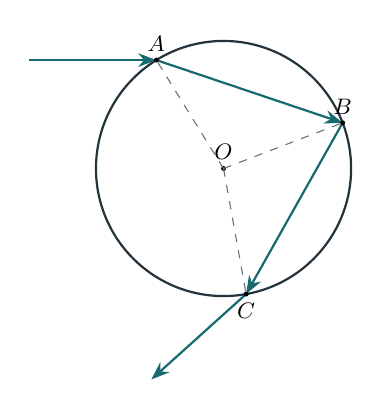
\begin{tikzpicture}[scale=.9,transform shape]
\draw[object] (0.00000,0.00000) circle(1.80000);\draw[motion] (-2.74821,1.53000)--(-0.94821,1.53000);
\draw[motion] (-0.94821,1.53000)--(1.68045,0.64505);
\draw[motion] (1.68045,0.64505)--(0.31909,-1.77149);
\draw[motion] (0.31909,-1.77149)--(-1.01859,-2.97591);\fill (0.00000,0.00000) circle(.035);\node[above] at (0.00000,0.00000) {$O$};\fill (-0.94821,1.53000) circle(.035);\node[above] at (-0.94821,1.53000) {$A$};\draw[guide] (0.00000,0.00000)--(-0.94821,1.53000);\fill (1.68045,0.64505) circle(.035);\node[above] at (1.68045,0.64505) {$B$};\draw[guide] (0.00000,0.00000)--(1.68045,0.64505);\fill (0.31909,-1.77149) circle(.035);\node[below] at (0.31909,-1.77149) {$C$};\draw[guide] (0.00000,0.00000)--(0.31909,-1.77149);
\end{tikzpicture}
\figcaption{图光1.3\quad 一折射、一次内反射、再折射的光支}
\end{minipage}\end{center}

\Needspace{8\baselineskip}

\pdfbookmark[3]{题型定位}{q3-h0}

\subsection*{题型定位}

用两条滴内弦的等腰三角形统一三个内部角，先比较临界角排除严格全反射，再累计A、B、C三次转折。驻值方程、平方正支、参数范围和端点斜率分别检验；推广折射率或反射次数时，明确累计偏转量与最终射线夹角的区别。

\Needspace{8\baselineskip}

\pdfbookmark[3]{知识点}{q3-h1}

\subsection*{知识点}

\begin{itemize}
\item 滴内只有AB、BC两条弦；OA、OB、OC半径相等，反射定律使两条弦各端与半径的锐角都等于r。
\item 入口$\sin\theta=n\sin r$限制B处$r<i_c$，因此内反射光只是分束后的一支，未追踪的B透射支也携带能量。
\item A、C两次折射各转$\theta-r$，B反射转$\pi-2r$，按同一转向累计得$\delta=\pi+2\theta-4r$。
\item 在$[0,\pi/2)$内$n\cos r$取正平方根，驻值式平方后还须检验$\cos^2\theta$的可取范围。
\item $\delta'$严格增加，$1<n<2$唯一内部极小，$n=2$驻值退端点，$n>2$无内部极值。
\item 驻值附近的二阶角度聚集使用弧度，方向聚集、反射率与观测亮度不能互相替代。
\end{itemize}

\Needspace{8\baselineskip}

\pdfbookmark[3]{物理图像}{q3-h2}

\subsection*{物理图像}

A图给真实的A入射、AB传播、B分束、BC传播和C出射，分别画半径法线与角弧；入射角不悬空标在别处。B图仅平移四个方向箭头到共同起点，用三段转角相加，另标与反向入射轴的$\rho$。C图用实际函数比较$n=4/3,2,2.2$，区分内部先降后升与端点单调情形；A图所取$\sin\theta=0.85$是几何示例，不冒充驻值数据。

\Needspace{8\baselineskip}

\pdfbookmark[3]{解题入口}{q3-h3}

\subsection*{解题入口}

先在A图写$\triangle OAB$与$\triangle OBC$的底角，不能独立猜B的入射角。用入口Snell先判断反射性质，再到B图逐次转动方向箭头，确定累计偏向。微分时先确认根号正支，解驻值后再查n范围、端点斜率和唯一性，最后以C图核对各分支。

\Needspace{8\baselineskip}

\Needspace{18\baselineskip}
\pdfbookmark[3]{标准解法}{q3-h4}

\subsection*{标准解法}


解图光1.3A中的两条弦AB、BC依次连接入射点$A$、反射点$B$与出射点$C$。由于这些点都在同一个圆周上，弦与两端半径组成等腰三角形，故光线在$B$处的入射角也等于$r$。入口折射定律为
\[
\sin\theta=n\sin r.
\]
对$0\le\theta<90^\circ$，有
\[
\sin r=\frac{\sin\theta}{n}<\frac1n,\qquad
r<\arcsin(1/n)=i_c.
\]
几何中的等角可分别落实到两条弦：$\triangle OAB$给$\angle OAB=\angle ABO=r$，反射定律又给$\angle OBC=r$，再由$\triangle OBC$得$\angle BCO=r$。所以C处的内部入射角仍为r，外部折射角也回到$\theta$。这既说明B的全反射比较为何能使用入口数据，也说明最后一次偏折为何与第一次相同。

因此$B$处不满足全反射条件，只发生部分反射；另一部分能量会在$B$直接透出。本题继续追踪反射支，透射支携带的能量则从该处离开水滴。
\begin{center}\begin{minipage}{.98\linewidth}\centering
\begin{tikzpicture}[scale=.9,font=\small]
\draw[object](0,0)circle(1.8);
\coordinate(A)at(-0.94820884,1.53000000);\coordinate(B)at(1.68044887,0.64505162);\coordinate(C)at(0.31909079,-1.77149120);
\draw[motion](-2.74820884,1.53000000)--(A)--(B)--(C)--(-0.90711222,-2.87554109);
\draw[force](B)--(2.95469354,-0.32257462);
\draw[guide](0,0)--(-1.30852820,2.11140000);\draw[guide](0,0)--(B);\draw[guide](0,0)--(0.44034529,-2.44465785);
\node[below left]at(0,0){$O$};
\node[above left]at(A){$A$};\node[above right]at(B){$B$};\node[right]at(C){$C$};
\draw ($(A)+(121.78833062:.43)$)arc(121.78833062:180:.43);\node at(-1.55,1.9){$\theta$};
\draw ($(A)+(-58.21166938:.43)$)arc(-58.21166938:-18.60601699:.43);\node at(-.46,1.12){$r$};
\draw ($(B)+(161.39398301:.4)$)arc(161.39398301:200.99963540:.4);\node at(1.08,.65){$r$};
\draw ($(B)+(200.99963540:.4)$)arc(200.99963540:240.60528780:.4);\node at(1.18,.15){$r$};
\draw ($(C)+(-138.00072919:.4)$)arc(-138.00072919:-79.78905981:.4);\node at(.08,-2.34){$\theta$};
\node[below right]at(2.75,-1.0){B处透射支};
\node[align=left,anchor=west]at(4.15,.45){$OA=OB=OC$\\两条滴内弦：AB、BC\\A折射，B部分反射，C折射\\每条弦两端夹半径角相同\\图取$n=4/3,\ \sin\theta=0.85$\\几何示例，非驻值角图};
\end{tikzpicture}
\figcaption{解图光1.3A\quad 同一球面弦两端角相等，内反射另有透射支}
\end{minipage}\end{center}
\begin{center}\begin{minipage}{.97\linewidth}\centering
\begin{tikzpicture}[scale=.82,font=\small]
\draw[motion](0,0)--(2.3,0)node[above]{$\vect k_0$};
\draw[motion](0,0)--(2.17979029,-0.73383533) node[right]{$\vect k_1$};
\draw[motion](0,0)--(-1.12889370,-2.00389596) node[below]{$\vect k_2$};
\draw[motion](0,0)--(-1.70925268,-1.53897864) node[above]{$\vect k_3$};
\draw[guide](0,0)--(-2.6,0)node[above left]{反向入射};
\draw(1.3,0)arc(0:-18.60601699:1.3);\node at(1.6,-.26){A};
\draw(-18.60601699:1.65)arc(-18.60601699:-119.39471220:1.65);\node at(.72,-1.87){B};
\draw(-119.39471220:1.12)arc(-119.39471220:-138.00072919:1.12);\node at(-1,-1.25){C};
\draw[->,>=Stealth,color=accent](2.7,0)arc(0:-138.00072919:2.7);
\draw[->,>=Stealth,color=warm](-2.7,0)arc(180:221.99927081:2.7);
\node[below]at(.4,-2.95){$\delta$};\node at(-3,-1.1){$\rho$};
\node[align=left,anchor=west]at(4.15,-1.1){仅平移方向箭头，未增加传播段\\A：$\theta-r$\\B：$\pi-2r$\\C：$\theta-r$\\$\delta=\pi+2\theta-4r$\\水滴示例的反向观察角$\rho=\pi-\delta$};
\end{tikzpicture}
\figcaption{解图光1.3B　三次转折的方向比较。将四个传播方向平移到共同起点，只比较转角；实际传播路径仍是A至B至C。}
\end{minipage}\end{center}


沿有向光路逐次累计偏折：入射折射贡献$\theta-r$，内反射贡献$\pi-2r$，出射折射再贡献$\theta-r$，故
\[
\delta(\theta)=\pi+2\theta-4r(\theta),\qquad
r=\arcsin(\sin\theta/n).
\]
解图光1.3B中$\vect k_0,\vect k_1,\vect k_2,\vect k_3$分别是入射、AB、BC和C出射的方向，不是从圆心再次发出的光线。三个顺时针转折相加后取正的累计大小作为$\delta$；若它超过$\pi$，仍保留累计量，不在求极值途中改换为另一夹角。

在水滴通常的$0<\delta<\pi$分支，还可令反向观察角$\rho=\pi-\delta$、辅助半角$\chi=\rho/2$。由两次折射和一次反射的方向关系，$\chi=2r-\theta$，于是
\[
\delta=\pi-2\chi,\qquad \chi=2r-\theta,
\]
同样给$\delta=\pi-4r+2\theta$。只有在明确选定此分支后，$\rho$才直接是与反向入射方向的正夹角；一般折射率推广仍用前述累计定义。

对入口折射式求导，
\[
\cos\theta=n\cos r\,\frac{\dd r}{\dd\theta},
\qquad
\frac{\dd r}{\dd\theta}
=\frac{\cos\theta}{\sqrt{n^2-\sin^2\theta}}.
\]
将两项通分，分子中的平方项相消：
\[
n\cos r=n\sqrt{1-\sin^2r}
=\sqrt{n^2-\sin^2\theta}>0 .
\]
这里$\theta,r$都取$[0,\pi/2)$内的角，故平方根取正支，后面平方驻值式才不会额外引入负号解。

驻值条件为
\[
\frac{\dd\delta}{\dd\theta}
=2-\frac{4\cos\theta}{\sqrt{n^2-\sin^2\theta}}=0.
\]
两端均为非负数，可以平方并整理：
\[
4\cos^2\theta=n^2-\sin^2\theta
=n^2-1+\cos^2\theta,
\qquad
\boxed{\cos^2\theta=\frac{n^2-1}{3}}.
\]
还应检验它确实是极小值。令$g=\cos\theta/\sqrt{n^2-\sin^2\theta}$，则
\[
g'=-\frac{(n^2-1)\sin\theta}
{(n^2-\sin^2\theta)^{3/2}},
\qquad
\delta''=\frac{4(n^2-1)\sin\theta}
{(n^2-\sin^2\theta)^{3/2}}>0.
\]
故$1<n<2$时存在唯一内部极小值。$n=2$时驻值退至$\theta=0$端点；$n>2$时$\delta'(0)>0$且$\delta''\ge0$，最小值在正入射端点，不存在内部驻值。对水取$n=4/3$，得到$\theta\approx59.39^\circ$、$r\approx40.20^\circ$、$\delta_{\min}\approx137.97^\circ$，相对于反向入射方向的夹角约为$42.03^\circ$。


唯一性还可直接从端点斜率看出。对固定$n>1$，
\[
\delta'(0)=2-\frac4n,\qquad
\lim_{\theta\to(\pi/2)^-}\delta'(\theta)=2 .
\]
又因$\delta''(\theta)>0$对$0<\theta<\pi/2$成立，$\delta'$严格增加。当$1<n<2$时，它由负到正，恰过零一次；当$n=2$时只在左端点为零，随后为正；当$n>2$时从左端已为正。因此不能只凭$\cos^2\theta$形式就把所有$n>1$都判作有内部极小值。

对$n=4/3$，中间数值依次为
\[
\begin{gathered}
\cos^2\theta_*=\frac7{27},\qquad
\theta_*=59.391102^\circ,\qquad
r_*=40.202966^\circ,\\
\chi_*=2r_*-\theta_*=21.014829^\circ,\\
\delta_{\min}=180^\circ-2\chi_*
=137.970341^\circ,\qquad
\rho_*=42.029659^\circ.
\end{gathered}
\]
B处入射角40.20度仍小于水向空气的临界角48.59度，所以方向聚集与全反射是两个不同现象。极值来自相邻入射角的出射方向变得接近，不要求反射率等于1。


\begin{center}\begin{minipage}{.97\linewidth}\centering
\begin{tikzpicture}[x=.075cm,y=.027cm,font=\small]
\draw[axis](0,0)--(96,0)node[right]{$\theta/(^\circ)$};
\draw[axis](0,0)--(0,145)node[above]{$\delta/(^\circ)$};
\foreach \x in {0,30,60,90}{\draw(\x,0)--(\x,-2)node[below]{$\x$};}
\foreach \y/\v in {20/140,60/180,100/220,140/260}{\draw(0,\y)--(-1.5,\y)node[left]{$\v$};}
\draw[traj]plot coordinates {(0.00000000,60.00000000) (0.50000000,59.50000833) (1.00000000,59.00006664) (1.50000000,58.50022492) (2.00000000,58.00053321) (2.50000000,57.50104158) (3.00000000,57.00180015) (3.50000000,56.50285914) (4.00000000,56.00426887) (4.50000000,55.50607973) (5.00000000,55.00834228) (5.50000000,54.51110718) (6.00000000,54.01442528) (6.50000000,53.51834757) (7.00000000,53.02292525) (7.50000000,52.52820972) (8.00000000,52.03425259) (8.50000000,51.54110571) (9.00000000,51.04882118) (9.50000000,50.55745138) (10.00000000,50.06704895) (10.50000000,49.57766686) (11.00000000,49.08935838) (11.50000000,48.60217711) (12.00000000,48.11617701) (12.50000000,47.63141242) (13.00000000,47.14793803) (13.50000000,46.66580897) (14.00000000,46.18508078) (14.50000000,45.70580942) (15.00000000,45.22805132) (15.50000000,44.75186339) (16.00000000,44.27730301) (16.50000000,43.80442810) (17.00000000,43.33329708) (17.50000000,42.86396893) (18.00000000,42.39650319) (18.50000000,41.93096001) (19.00000000,41.46740010) (19.50000000,41.00588483) (20.00000000,40.54647620) (20.50000000,40.08923687) (21.00000000,39.63423019) (21.50000000,39.18152021) (22.00000000,38.73117171) (22.50000000,38.28325019) (23.00000000,37.83782196) (23.50000000,37.39495408) (24.00000000,36.95471442) (24.50000000,36.51717171) (25.00000000,36.08239550) (25.50000000,35.65045623) (26.00000000,35.22142523) (26.50000000,34.79537475) (27.00000000,34.37237799) (27.50000000,33.95250910) (28.00000000,33.53584322) (28.50000000,33.12245652) (29.00000000,32.71242617) (29.50000000,32.30583044) (30.00000000,31.90274865) (30.50000000,31.50326124) (31.00000000,31.10744978) (31.50000000,30.71539700) (32.00000000,30.32718679) (32.50000000,29.94290427) (33.00000000,29.56263579) (33.50000000,29.18646893) (34.00000000,28.81449257) (34.50000000,28.44679690) (35.00000000,28.08347343) (35.50000000,27.72461502) (36.00000000,27.37031594) (36.50000000,27.02067184) (37.00000000,26.67577982) (37.50000000,26.33573842) (38.00000000,26.00064768) (38.50000000,25.67060915) (39.00000000,25.34572590) (39.50000000,25.02610257) (40.00000000,24.71184538) (40.50000000,24.40306216) (41.00000000,24.09986237) (41.50000000,23.80235711) (42.00000000,23.51065920) (42.50000000,23.22488312) (43.00000000,22.94514510) (43.50000000,22.67156310) (44.00000000,22.40425686) (44.50000000,22.14334790) (45.00000000,21.88895954) (45.50000000,21.64121696) (46.00000000,21.40024713) (46.50000000,21.16617893) (47.00000000,20.93914310) (47.50000000,20.71927226) (48.00000000,20.50670096) (48.50000000,20.30156564) (49.00000000,20.10400468) (49.50000000,19.91415842) (50.00000000,19.73216911) (50.50000000,19.55818097) (51.00000000,19.39234017) (51.50000000,19.23479483) (52.00000000,19.08569503) (52.50000000,18.94519282) (53.00000000,18.81344218) (53.50000000,18.69059903) (54.00000000,18.57682122) (54.50000000,18.47226854) (55.00000000,18.37710267) (55.50000000,18.29148715) (56.00000000,18.21558741) (56.50000000,18.14957071) (57.00000000,18.09360611) (57.50000000,18.04786445) (58.00000000,18.01251830) (58.50000000,17.98774193) (59.00000000,17.97371127) (59.50000000,17.97060383) (60.00000000,17.97859869) (60.50000000,17.99787641) (61.00000000,18.02861899) (61.50000000,18.07100977) (62.00000000,18.12523339) (62.50000000,18.19147569) (63.00000000,18.26992366) (63.50000000,18.36076530) (64.00000000,18.46418956) (64.50000000,18.58038624) (65.00000000,18.70954587) (65.50000000,18.85185961) (66.00000000,19.00751914) (66.50000000,19.17671652) (67.00000000,19.35964405) (67.50000000,19.55649418) (68.00000000,19.76745934) (68.50000000,19.99273178) (69.00000000,20.23250347) (69.50000000,20.48696589) (70.00000000,20.75630987) (70.50000000,21.04072546) (71.00000000,21.34040174) (71.50000000,21.65552662) (72.00000000,21.98628668) (72.50000000,22.33286699) (73.00000000,22.69545087) (73.50000000,23.07421975) (74.00000000,23.46935295) (74.50000000,23.88102747) (75.00000000,24.30941779) (75.50000000,24.75469565) (76.00000000,25.21702986) (76.50000000,25.69658607) (77.00000000,26.19352657) (77.50000000,26.70801009) (78.00000000,27.24019152) (78.50000000,27.79022180) (79.00000000,28.35824762) (79.50000000,28.94441125) (80.00000000,29.54885033) (80.50000000,30.17169767) (81.00000000,30.81308103) (81.50000000,31.47312295) (82.00000000,32.15194055) (82.50000000,32.84964531) (83.00000000,33.56634298) (83.50000000,34.30213330) (84.00000000,35.05710991) (84.50000000,35.83136018) (85.00000000,36.62496504) (85.50000000,37.43799889) (86.00000000,38.27052941) (86.50000000,39.12261749) (87.00000000,39.99431711) (87.50000000,40.88567526) (88.00000000,41.79673182) (88.50000000,42.72751953) (89.00000000,43.67806391) (89.50000000,44.64838322) (90.00000000,45.63848844)};
\draw[color=warm,line width=1pt]plot coordinates {(0.00000000,60.00000000) (0.50000000,60.00000952) (1.00000000,60.00007616) (1.50000000,60.00025703) (2.00000000,60.00060928) (2.50000000,60.00119005) (3.00000000,60.00205652) (3.50000000,60.00326588) (4.00000000,60.00487536) (4.50000000,60.00694224) (5.00000000,60.00952382) (5.50000000,60.01267747) (6.00000000,60.01646060) (6.50000000,60.02093068) (7.00000000,60.02614526) (7.50000000,60.03216194) (8.00000000,60.03903841) (8.50000000,60.04683242) (9.00000000,60.05560184) (9.50000000,60.06540459) (10.00000000,60.07629871) (10.50000000,60.08834234) (11.00000000,60.10159372) (11.50000000,60.11611120) (12.00000000,60.13195324) (12.50000000,60.14917843) (13.00000000,60.16784548) (13.50000000,60.18801322) (14.00000000,60.20974065) (14.50000000,60.23308685) (15.00000000,60.25811110) (15.50000000,60.28487278) (16.00000000,60.31343146) (16.50000000,60.34384684) (17.00000000,60.37617879) (17.50000000,60.41048735) (18.00000000,60.44683271) (18.50000000,60.48527524) (19.00000000,60.52587549) (19.50000000,60.56869419) (20.00000000,60.61379224) (20.50000000,60.66123074) (21.00000000,60.71107096) (21.50000000,60.76337438) (22.00000000,60.81820266) (22.50000000,60.87561768) (23.00000000,60.93568150) (23.50000000,60.99845639) (24.00000000,61.06400482) (24.50000000,61.13238947) (25.00000000,61.20367324) (25.50000000,61.27791922) (26.00000000,61.35519074) (26.50000000,61.43555131) (27.00000000,61.51906470) (27.50000000,61.60579485) (28.00000000,61.69580597) (28.50000000,61.78916243) (29.00000000,61.88592887) (29.50000000,61.98617013) (30.00000000,62.08995126) (30.50000000,62.19733754) (31.00000000,62.30839448) (31.50000000,62.42318779) (32.00000000,62.54178342) (32.50000000,62.66424750) (33.00000000,62.79064642) (33.50000000,62.92104676) (34.00000000,63.05551532) (34.50000000,63.19411909) (35.00000000,63.33692530) (35.50000000,63.48400137) (36.00000000,63.63541492) (36.50000000,63.79123377) (37.00000000,63.95152593) (37.50000000,64.11635961) (38.00000000,64.28580322) (38.50000000,64.45992532) (39.00000000,64.63879467) (39.50000000,64.82248020) (40.00000000,65.01105100) (40.50000000,65.20457632) (41.00000000,65.40312558) (41.50000000,65.60676834) (42.00000000,65.81557428) (42.50000000,66.02961324) (43.00000000,66.24895519) (43.50000000,66.47367018) (44.00000000,66.70382841) (44.50000000,66.93950015) (45.00000000,67.18075578) (45.50000000,67.42766575) (46.00000000,67.68030059) (46.50000000,67.93873088) (47.00000000,68.20302724) (47.50000000,68.47326035) (48.00000000,68.74950089) (48.50000000,69.03181959) (49.00000000,69.32028713) (49.50000000,69.61497422) (50.00000000,69.91595153) (50.50000000,70.22328967) (51.00000000,70.53705921) (51.50000000,70.85733067) (52.00000000,71.18417444) (52.50000000,71.51766085) (53.00000000,71.85786009) (53.50000000,72.20484222) (54.00000000,72.55867714) (54.50000000,72.91943460) (55.00000000,73.28718416) (55.50000000,73.66199516) (56.00000000,74.04393672) (56.50000000,74.43307772) (57.00000000,74.82948679) (57.50000000,75.23323225) (58.00000000,75.64438215) (58.50000000,76.06300418) (59.00000000,76.48916572) (59.50000000,76.92293376) (60.00000000,77.36437491) (60.50000000,77.81355536) (61.00000000,78.27054090) (61.50000000,78.73539682) (62.00000000,79.20818796) (62.50000000,79.68897865) (63.00000000,80.17783271) (63.50000000,80.67481338) (64.00000000,81.17998335) (64.50000000,81.69340472) (65.00000000,82.21513895) (65.50000000,82.74524686) (66.00000000,83.28378859) (66.50000000,83.83082361) (67.00000000,84.38641065) (67.50000000,84.95060770) (68.00000000,85.52347198) (68.50000000,86.10505990) (69.00000000,86.69542707) (69.50000000,87.29462824) (70.00000000,87.90271731) (70.50000000,88.51974725) (71.00000000,89.14577013) (71.50000000,89.78083709) (72.00000000,90.42499826) (72.50000000,91.07830280) (73.00000000,91.74079886) (73.50000000,92.41253352) (74.00000000,93.09355282) (74.50000000,93.78390168) (75.00000000,94.48362393) (75.50000000,95.19276226) (76.00000000,95.91135819) (76.50000000,96.63945207) (77.00000000,97.37708305) (77.50000000,98.12428903) (78.00000000,98.88110670) (78.50000000,99.64757147) (79.00000000,100.42371746) (79.50000000,101.20957750) (80.00000000,102.00518308) (80.50000000,102.81056436) (81.00000000,103.62575015) (81.50000000,104.45076788) (82.00000000,105.28564359) (82.50000000,106.13040191) (83.00000000,106.98506607) (83.50000000,107.84965784) (84.00000000,108.72419757) (84.50000000,109.60870414) (85.00000000,110.50319497) (85.50000000,111.40768598) (86.00000000,112.32219163) (86.50000000,113.24672486) (87.00000000,114.18129712) (87.50000000,115.12591834) (88.00000000,116.08059694) (88.50000000,117.04533981) (89.00000000,118.02015230) (89.50000000,119.00503827) (90.00000000,120.00000000)};
\draw[color=muted,line width=1pt]plot coordinates {(0.00000000,60.00000000) (0.50000000,60.09091825) (1.00000000,60.18189142) (1.50000000,60.27297445) (2.00000000,60.36422229) (2.50000000,60.45568987) (3.00000000,60.54743216) (3.50000000,60.63950415) (4.00000000,60.73196083) (4.50000000,60.82485725) (5.00000000,60.91824844) (5.50000000,61.01218951) (6.00000000,61.10673558) (6.50000000,61.20194181) (7.00000000,61.29786340) (7.50000000,61.39455561) (8.00000000,61.49207374) (8.50000000,61.59047315) (9.00000000,61.68980923) (9.50000000,61.79013747) (10.00000000,61.89151339) (10.50000000,61.99399258) (11.00000000,62.09763071) (11.50000000,62.20248352) (12.00000000,62.30860682) (12.50000000,62.41605649) (13.00000000,62.52488850) (13.50000000,62.63515891) (14.00000000,62.74692384) (14.50000000,62.86023953) (15.00000000,62.97516229) (15.50000000,63.09174854) (16.00000000,63.21005477) (16.50000000,63.33013759) (17.00000000,63.45205371) (17.50000000,63.57585994) (18.00000000,63.70161318) (18.50000000,63.82937047) (19.00000000,63.95918892) (19.50000000,64.09112578) (20.00000000,64.22523839) (20.50000000,64.36158423) (21.00000000,64.50022087) (21.50000000,64.64120602) (22.00000000,64.78459748) (22.50000000,64.93045319) (23.00000000,65.07883120) (23.50000000,65.22978969) (24.00000000,65.38338696) (24.50000000,65.53968141) (25.00000000,65.69873160) (25.50000000,65.86059618) (26.00000000,66.02533394) (26.50000000,66.19300378) (27.00000000,66.36366474) (27.50000000,66.53737596) (28.00000000,66.71419673) (28.50000000,66.89418642) (29.00000000,67.07740457) (29.50000000,67.26391080) (30.00000000,67.45376485) (30.50000000,67.64702660) (31.00000000,67.84375603) (31.50000000,68.04401323) (32.00000000,68.24785839) (32.50000000,68.45535184) (33.00000000,68.66655399) (33.50000000,68.88152536) (34.00000000,69.10032656) (34.50000000,69.32301833) (35.00000000,69.54966146) (35.50000000,69.78031686) (36.00000000,70.01504551) (36.50000000,70.25390849) (37.00000000,70.49696694) (37.50000000,70.74428209) (38.00000000,70.99591522) (38.50000000,71.25192769) (39.00000000,71.51238091) (39.50000000,71.77733634) (40.00000000,72.04685550) (40.50000000,72.32099994) (41.00000000,72.59983125) (41.50000000,72.88341103) (42.00000000,73.17180094) (42.50000000,73.46506262) (43.00000000,73.76325773) (43.50000000,74.06644792) (44.00000000,74.37469485) (44.50000000,74.68806013) (45.00000000,75.00660539) (45.50000000,75.33039218) (46.00000000,75.65948204) (46.50000000,75.99393644) (47.00000000,76.33381677) (47.50000000,76.67918440) (48.00000000,77.03010056) (48.50000000,77.38662641) (49.00000000,77.74882302) (49.50000000,78.11675132) (50.00000000,78.49047212) (50.50000000,78.87004609) (51.00000000,79.25553377) (51.50000000,79.64699550) (52.00000000,80.04449148) (52.50000000,80.44808169) (53.00000000,80.85782592) (53.50000000,81.27378377) (54.00000000,81.69601456) (54.50000000,82.12457742) (55.00000000,82.55953119) (55.50000000,83.00093445) (56.00000000,83.44884548) (56.50000000,83.90332229) (57.00000000,84.36442255) (57.50000000,84.83220359) (58.00000000,85.30672242) (58.50000000,85.78803567) (59.00000000,86.27619960) (59.50000000,86.77127007) (60.00000000,87.27330252) (60.50000000,87.78235199) (61.00000000,88.29847303) (61.50000000,88.82171978) (62.00000000,89.35214586) (62.50000000,89.88980442) (63.00000000,90.43474809) (63.50000000,90.98702897) (64.00000000,91.54669860) (64.50000000,92.11380797) (65.00000000,92.68840748) (65.50000000,93.27054694) (66.00000000,93.86027553) (66.50000000,94.45764179) (67.00000000,95.06269362) (67.50000000,95.67547824) (68.00000000,96.29604218) (68.50000000,96.92443127) (69.00000000,97.56069060) (69.50000000,98.20486454) (70.00000000,98.85699667) (70.50000000,99.51712983) (71.00000000,100.18530604) (71.50000000,100.86156650) (72.00000000,101.54595161) (72.50000000,102.23850089) (73.00000000,102.93925304) (73.50000000,103.64824583) (74.00000000,104.36551618) (74.50000000,105.09110008) (75.00000000,105.82503258) (75.50000000,106.56734780) (76.00000000,107.31807891) (76.50000000,108.07725810) (77.00000000,108.84491656) (77.50000000,109.62108450) (78.00000000,110.40579110) (78.50000000,111.19906452) (79.00000000,112.00093186) (79.50000000,112.81141919) (80.00000000,113.63055149) (80.50000000,114.45835267) (81.00000000,115.29484555) (81.50000000,116.14005186) (82.00000000,116.99399219) (82.50000000,117.85668604) (83.00000000,118.72815174) (83.50000000,119.60840652) (84.00000000,120.49746642) (84.50000000,121.39534637) (85.00000000,122.30206009) (85.50000000,123.21762015) (86.00000000,124.14203794) (86.50000000,125.07532368) (87.00000000,126.01748637) (87.50000000,126.96853384) (88.00000000,127.92847273) (88.50000000,128.89730845) (89.00000000,129.87504523) (89.50000000,130.86168609) (90.00000000,131.85723284)};
\draw[guide](59.39110234,0)--(59.39110234,17.97034113)--(0,17.97034113);
\fill[accent](59.39110234,17.97034113)circle(.055cm);
\node[above left]at(59.39110234,17.97034113){$(\theta_*,\delta_{\min})$};
\foreach \y in {45.63848844,120.00000000,131.85723284}{\draw[fill=white](90,\y)circle(.045cm);}
\node[align=left,anchor=west]at(108,105){{\color{accent}$n=4/3$：唯一内部极小}\\{\color{warm}$n=2$：驻值退到端点}\\{\color{muted}$n=2.2$：全程递增}\\$\delta$按同一方向累计\\90度处空心点只示掠射极限};
\end{tikzpicture}
\figcaption{解图光1.3C　三种折射率的累计偏转曲线。内部极小值、端点退化和全程递增分别对应不同参数范围，不能只解驻值方程。}
\end{minipage}\end{center}

解图光1.3C的蓝线在$\theta_*$两侧先降后升；棕线与灰线则从端点开始上升。纵轴为累计$\delta$，部分曲线大于180度时没有折回，因而与上面的$n\ge2$单调性判断一致。若要由实际射线方向报告较小夹角，应在累计光路已确定后另作方向取模，不能混在同一极值函数内。

在水滴驻值附近，若角度统一用弧度，
\[
\delta-\delta_{\min}
=\frac12\delta''(\theta_*)(\theta-\theta_*)^2
+O((\theta-\theta_*)^3),\qquad
\delta''(\theta_*)\simeq2.53546 .
\]
一次项为零，所以两侧小幅改变入口角都可给几乎相同的出射方向。该局部展开解释了角度聚集，但不单独给出光强，也不把B处的部分反射改成全反射。



\Needspace{8\baselineskip}

\pdfbookmark[3]{关键洞察}{q3-h5}

\subsection*{关键洞察}

特定出射方向附近的角度聚集由$\delta'(\theta_*)=0$形成，并不要求B处反射率为1。有限入射角始终给$r<i_c$；与此同时，是否照到驻值所需的入口位置、以及最后采用累计角还是较小夹角，也都影响结论的适用范围。

\Needspace{8\baselineskip}

\pdfbookmark[3]{易错点}{q3-h6}

\subsection*{易错点}

\begin{itemize}
\item 把一次内反射说成三条滴内弦，或把B处$r$当作可独立调节的入射角。
\item 看到内反射就写全反射，漏掉入口Snell所给的严格$r<i_c$。
\item 只猜图外夹角，颠倒两次折射的转向，写错$\pi+2\theta-4r$。
\item 在n推广后把超过$\pi$的累计量突然折回较小角，却仍套同一个极值判别。
\item 平方后不查$\cos^2\theta\in(0,1)$，或把$n=2$端点称作内部极小。
\item 二阶展开把1度直接代成1弧度，或把角聚集误说成反射能量全都保留。
\end{itemize}

\Needspace{8\baselineskip}

\pdfbookmark[3]{课堂讲解建议}{q3-h7}

\subsection*{课堂讲解建议}

先沿A图数清两条弦和三次转折，逐个指出角弧的顶点及法线。让学生用两组等腰三角形证明B、C内部角都为r，再把入口式带到B排除严格全反射；图中的棕色透射支解释了未选取能量从哪里离开。

把四个传播方向搬到B图共同起点，实际转动箭头累计A、B、C的转角。此图只比较方向，不增加传播段。明确水滴分支的$\delta$与反向观察角$\rho$互补，再说明累计量的推广定义，防止在$n\ge2$情形悄悄更换角度。

驻值求解后，让学生先给n的可取范围，再算$\delta'(0)$及右端斜率，用严格增加的$\delta'$证明唯一性。C图三条实际曲线作最后核对，特别追问$n=2$为什么只在端点零斜率。数值例子要把59.39度、137.97度和42.03度分别对应到入口、累计偏向和观察方向。

最后让入口偏离驻值1度，先换弧度再估二阶偏向变化；再用窄束只照到$0.80R$的反例，区分函数有驻值与实际光束可达。课堂的能量、几何、参数范围和光支选择都要有具体图中对象，不能只留下一个驻值公式。

\Needspace{8\baselineskip}

\Needspace{18\baselineskip}
\pdfbookmark[3]{变式训练}{q3-h8}

\subsection*{变式训练}

\begin{enumerate}
\Needspace{7\baselineskip}
\item 取$n=\sqrt2$。驻值满足$\cos^2\theta=1/3$，得$\theta\approx54.74^\circ$、$r\approx35.26^\circ$，故$\delta_{\min}\approx148.41^\circ$。\par 反向观察角为$180^\circ-148.41^\circ\simeq31.59^\circ$。此时$r_*\simeq35.26^\circ$，仍小于$i_c=45^\circ$；若用全反射解释极小偏向，就会与这一明确数值比较冲突。图C的思路是先判断导数过零，再检查反射条件，二者各自独立。
\begin{center}\begin{minipage}{.98\linewidth}\centering
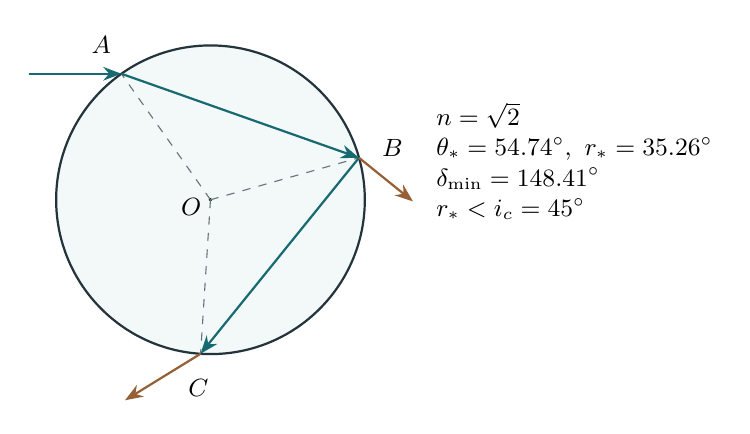
\begin{tikzpicture}[scale=.98]\fill[accent!5](0,0)circle(2);\draw[object](0,0)circle(2);\fill(0,0)circle(.025);\coordinate(A)at(-1.15470054,1.63299316);\draw[guide](0.00000000,0.00000000)--(-1.15470054,1.63299316);\coordinate(B)at(1.92450090,0.54433105);\draw[guide](0.00000000,0.00000000)--(1.92450090,0.54433105);\coordinate(C)at(-0.12830006,-1.99588053);\draw[guide](0.00000000,0.00000000)--(-0.12830006,-1.99588053);\node[fill=accent!5,inner sep=1pt]at(-.25,-.1){$O$};\draw[motion](-2.35470054,1.63299316)--(-1.15470054,1.63299316);\draw[motion](-1.15470054,1.63299316)--(1.92450090,0.54433105);\draw[motion](1.92450090,0.54433105)--(-0.12830006,-1.99588053);\coordinate(T)at(-1.10792969,-2.59823075);\draw[force](-0.12830006,-1.99588053)--(-1.10792969,-2.59823075);\node at(-1.41450816,2.00041662){\(A\)};\node at(2.35751360,0.66680554){\(B\)};\node at(-0.15716757,-2.44495365){\(C\)};\coordinate(L)at(2.62450090,-0.02135437);\draw[force](1.92450090,0.54433105)--(2.62450090,-0.02135437);\node[align=left,anchor=west]at(2.8,.5){$n=\sqrt2$\\$\theta_*=54.74^\circ,\ r_*=35.26^\circ$\\$\delta_{\min}=148.41^\circ$\\$r_*<i_c=45^\circ$};\end{tikzpicture}
\figcaption{变图光1.3V1\quad 一内反射支在折射率根号二时的真实光路}
\end{minipage}\end{center}
\par 图V1中$A$处折射后沿$AB$传播，在$B$处反射，最后从$C$透出。各半径给出局部法线，$B$处内部角仍为$r_*$。棕色的$B$处透射支存在，因$35.26^\circ<45^\circ$；偏向极小与这条支的反射率是否为一是两回事。
\Needspace{7\baselineskip}
\item 求两次内反射支的偏向函数。累计两次反射得$\delta_2=2\pi+2\theta-6r$；驻值要求$r'=1/3$，整理得$\cos^2\theta=(n^2-1)/8$，还须按所需的方向角取模。\par 内部驻值存在于$1<n<3$，因为右端必须介于0和1。对$n=4/3$得$\theta_*\simeq71.832^\circ,r_*\simeq45.448^\circ,\delta_2\simeq230.978^\circ$。这是同转向累计量；出射方向与反向入射轴的角约为$|\delta_2-\pi|\simeq50.978^\circ$，不可把230.978度直接当作两射线的较小夹角。
\begin{center}\begin{minipage}{.98\linewidth}\centering
\begin{tikzpicture}[scale=.98]\fill[accent!5](0,0)circle(2);\draw[object](0,0)circle(2);\fill(0,0)circle(.025);\coordinate(A)at(-0.62360956,1.90029238);\draw[guide](0.00000000,0.00000000)--(-0.62360956,1.90029238);\coordinate(B)at(1.89031649,0.65322550);\draw[guide](0.00000000,0.00000000)--(1.89031649,0.65322550);\coordinate(C)at(0.68268195,-1.87987908);\draw[guide](0.00000000,0.00000000)--(0.68268195,-1.87987908);\coordinate(D)at(-1.86898268,-0.71197173);\draw[guide](0.00000000,0.00000000)--(-1.86898268,-0.71197173);\node[fill=accent!5,inner sep=1pt]at(-.25,-.1){$O$};\draw[motion](-1.82360956,1.90029238)--(-0.62360956,1.90029238);\draw[motion](-0.62360956,1.90029238)--(1.89031649,0.65322550);\draw[motion](1.89031649,0.65322550)--(0.68268195,-1.87987908);\draw[motion](0.68268195,-1.87987908)--(-1.86898268,-0.71197173);\coordinate(T)at(-2.59304278,0.18146936);\draw[force](-1.86898268,-0.71197173)--(-2.59304278,0.18146936);\node at(-0.76392172,2.32785816){\(A\)};\node at(2.31563770,0.80020124){\(B\)};\node at(0.83628539,-2.30285187){\(C\)};\node at(-2.28950378,-0.87216536){\(D\)};\node[align=left,anchor=west]at(2.65,.2){$B,C$两处内反射\\$\theta_*=71.832^\circ$\\$\delta_2=230.978^\circ$\\反向观察角$50.978^\circ$};\end{tikzpicture}
\figcaption{变图光1.3V2\quad 两次内反射形成三条内部弦段}
\end{minipage}\end{center}
\par 图V2从$A$进入后依次沿$AB$、$BC$、$CD$传播，只有$B$、$C$两处反射。把同向转角累计得到$\delta_2$；最后实际出射方向已绕过$180^\circ$，所以观察角要由出射方向与反向入射轴再比较，不能把累计量直接当作较小夹角。
\Needspace{7\baselineskip}
\item 证明驻值附近的角聚集。以$\theta_*$展开，$\delta-\delta_{\min}=\tfrac12\delta''(\theta_*)(\theta-\theta_*)^2+\cdots$，一次项消失，说明相邻入口角对应的出射方向更接近。\par 对水取$\delta''(\theta_*)\simeq2.53546$，若入口改变量为1度，先化成$\pi/180$弧度，二阶估计给$\Delta\delta\simeq0.0003862\,{\rm rad}\simeq0.0221^\circ$。两侧入口角在一阶下都聚到同一方向，但更高阶项会使有限两侧偏移略不对称，不能由二阶式宣称它们永远完全相等。
\begin{center}\begin{minipage}{.98\linewidth}\centering
\begin{tikzpicture}[x=.85cm,y=11cm]\draw[axis](-3.4,0)--(3.5,0)node[right]{$(\theta-\theta_*)/^\circ$};\draw[axis](-3.4,0)--(-3.4,.28)node[above]{$(\delta-\delta_{\min})/^\circ$};\draw[traj]plot coordinates{(-3.00000000,0.19275734) (-2.95000000,0.18648702) (-2.90000000,0.18031702) (-2.85000000,0.17424751) (-2.80000000,0.16827866) (-2.75000000,0.16241064) (-2.70000000,0.15664362) (-2.65000000,0.15097777) (-2.60000000,0.14541326) (-2.55000000,0.13995026) (-2.50000000,0.13458895) (-2.45000000,0.12932949) (-2.40000000,0.12417205) (-2.35000000,0.11911682) (-2.30000000,0.11416395) (-2.25000000,0.10931362) (-2.20000000,0.10456601) (-2.15000000,0.09992128) (-2.10000000,0.09537961) (-2.05000000,0.09094117) (-2.00000000,0.08660614) (-1.95000000,0.08237468) (-1.90000000,0.07824697) (-1.85000000,0.07422318) (-1.80000000,0.07030349) (-1.75000000,0.06648807) (-1.70000000,0.06277709) (-1.65000000,0.05917074) (-1.60000000,0.05566917) (-1.55000000,0.05227257) (-1.50000000,0.04898111) (-1.45000000,0.04579496) (-1.40000000,0.04271431) (-1.35000000,0.03973932) (-1.30000000,0.03687017) (-1.25000000,0.03410704) (-1.20000000,0.03145010) (-1.15000000,0.02889953) (-1.10000000,0.02645549) (-1.05000000,0.02411818) (-1.00000000,0.02188776) (-0.95000000,0.01976442) (-0.90000000,0.01774832) (-0.85000000,0.01583964) (-0.80000000,0.01403857) (-0.75000000,0.01234527) (-0.70000000,0.01075993) (-0.65000000,0.00928272) (-0.60000000,0.00791382) (-0.55000000,0.00665341) (-0.50000000,0.00550167) (-0.45000000,0.00445876) (-0.40000000,0.00352488) (-0.35000000,0.00270020) (-0.30000000,0.00198489) (-0.25000000,0.00137914) (-0.20000000,0.00088313) (-0.15000000,0.00049703) (-0.10000000,0.00022102) (-0.05000000,0.00005529) (0.00000000,0.00000000) (0.05000000,0.00005535) (0.10000000,0.00022150) (0.15000000,0.00049865) (0.20000000,0.00088696) (0.25000000,0.00138662) (0.30000000,0.00199782) (0.35000000,0.00272072) (0.40000000,0.00355552) (0.45000000,0.00450238) (0.50000000,0.00556150) (0.55000000,0.00673305) (0.60000000,0.00801722) (0.65000000,0.00941418) (0.70000000,0.01092411) (0.75000000,0.01254721) (0.80000000,0.01428364) (0.85000000,0.01613360) (0.90000000,0.01809726) (0.95000000,0.02017480) (1.00000000,0.02236642) (1.05000000,0.02467228) (1.10000000,0.02709257) (1.15000000,0.02962748) (1.20000000,0.03227719) (1.25000000,0.03504187) (1.30000000,0.03792173) (1.35000000,0.04091692) (1.40000000,0.04402765) (1.45000000,0.04725409) (1.50000000,0.05059643) (1.55000000,0.05405485) (1.60000000,0.05762953) (1.65000000,0.06132066) (1.70000000,0.06512842) (1.75000000,0.06905300) (1.80000000,0.07309458) (1.85000000,0.07725334) (1.90000000,0.08152948) (1.95000000,0.08592317) (2.00000000,0.09043460) (2.05000000,0.09506395) (2.10000000,0.09981141) (2.15000000,0.10467717) (2.20000000,0.10966141) (2.25000000,0.11476431) (2.30000000,0.11998606) (2.35000000,0.12532685) (2.40000000,0.13078686) (2.45000000,0.13636628) (2.50000000,0.14206529) (2.55000000,0.14788408) (2.60000000,0.15382284) (2.65000000,0.15988175) (2.70000000,0.16606101) (2.75000000,0.17236078) (2.80000000,0.17878127) (2.85000000,0.18532266) (2.90000000,0.19198514) (2.95000000,0.19876889) (3.00000000,0.20567409)};\draw[guide]plot coordinates{(-3.00000000,0.19913478) (-2.95000000,0.19255227) (-2.90000000,0.18608039) (-2.85000000,0.17971914) (-2.80000000,0.17346852) (-2.75000000,0.16732853) (-2.70000000,0.16129917) (-2.65000000,0.15538044) (-2.60000000,0.14957235) (-2.55000000,0.14387488) (-2.50000000,0.13828804) (-2.45000000,0.13281184) (-2.40000000,0.12744626) (-2.35000000,0.12219131) (-2.30000000,0.11704700) (-2.25000000,0.11201331) (-2.20000000,0.10709026) (-2.15000000,0.10227784) (-2.10000000,0.09757604) (-2.05000000,0.09298488) (-2.00000000,0.08850435) (-1.95000000,0.08413444) (-1.90000000,0.07987517) (-1.85000000,0.07572653) (-1.80000000,0.07168852) (-1.75000000,0.06776114) (-1.70000000,0.06394439) (-1.65000000,0.06023827) (-1.60000000,0.05664278) (-1.55000000,0.05315792) (-1.50000000,0.04978369) (-1.45000000,0.04652010) (-1.40000000,0.04336713) (-1.35000000,0.04032479) (-1.30000000,0.03739309) (-1.25000000,0.03457201) (-1.20000000,0.03186156) (-1.15000000,0.02926175) (-1.10000000,0.02677256) (-1.05000000,0.02439401) (-1.00000000,0.02212609) (-0.95000000,0.01996879) (-0.90000000,0.01792213) (-0.85000000,0.01598610) (-0.80000000,0.01416070) (-0.75000000,0.01244592) (-0.70000000,0.01084178) (-0.65000000,0.00934827) (-0.60000000,0.00796539) (-0.55000000,0.00669314) (-0.50000000,0.00553152) (-0.45000000,0.00448053) (-0.40000000,0.00354017) (-0.35000000,0.00271045) (-0.30000000,0.00199135) (-0.25000000,0.00138288) (-0.20000000,0.00088504) (-0.15000000,0.00049784) (-0.10000000,0.00022126) (-0.05000000,0.00005532) (0.00000000,0.00000000) (0.05000000,0.00005532) (0.10000000,0.00022126) (0.15000000,0.00049784) (0.20000000,0.00088504) (0.25000000,0.00138288) (0.30000000,0.00199135) (0.35000000,0.00271045) (0.40000000,0.00354017) (0.45000000,0.00448053) (0.50000000,0.00553152) (0.55000000,0.00669314) (0.60000000,0.00796539) (0.65000000,0.00934827) (0.70000000,0.01084178) (0.75000000,0.01244592) (0.80000000,0.01416070) (0.85000000,0.01598610) (0.90000000,0.01792213) (0.95000000,0.01996879) (1.00000000,0.02212609) (1.05000000,0.02439401) (1.10000000,0.02677256) (1.15000000,0.02926175) (1.20000000,0.03186156) (1.25000000,0.03457201) (1.30000000,0.03739309) (1.35000000,0.04032479) (1.40000000,0.04336713) (1.45000000,0.04652010) (1.50000000,0.04978369) (1.55000000,0.05315792) (1.60000000,0.05664278) (1.65000000,0.06023827) (1.70000000,0.06394439) (1.75000000,0.06776114) (1.80000000,0.07168852) (1.85000000,0.07572653) (1.90000000,0.07987517) (1.95000000,0.08413444) (2.00000000,0.08850435) (2.05000000,0.09298488) (2.10000000,0.09757604) (2.15000000,0.10227784) (2.20000000,0.10709026) (2.25000000,0.11201331) (2.30000000,0.11704700) (2.35000000,0.12219131) (2.40000000,0.12744626) (2.45000000,0.13281184) (2.50000000,0.13828804) (2.55000000,0.14387488) (2.60000000,0.14957235) (2.65000000,0.15538044) (2.70000000,0.16129917) (2.75000000,0.16732853) (2.80000000,0.17346852) (2.85000000,0.17971914) (2.90000000,0.18608039) (2.95000000,0.19255227) (3.00000000,0.19913478)};\draw[guide](1,0)--(1,.0221267);\node[align=left,anchor=west]at(3.7,.17){实线：完整函数\\虚线：二次近似\\$1^\circ\mapsto0.0221^\circ$};\node[below]at(0,0){$0$};\end{tikzpicture}
\figcaption{变图光1.3V3\quad 驻值附近的实际曲线与二次近似}
\end{minipage}\end{center}
\par 图V3把入口角改变量与偏向改变量都以度显示，计算二次项时仍先换成弧度。蓝色完整函数与虚线二次式在零点相切；$1^\circ$入口改变量只给约$0.0221^\circ$偏向改变量。两侧完整曲线保留轻微不对称，没有把二次近似当作精确恒等式。
\Needspace{7\baselineskip}
\item 取$n=2$。此时$\delta'(0)=0$，但所有$\theta>0$都有$\delta'>0$，最小值为$\delta(0)=\pi$，应称端点最小而非有限角度处的虹角。
\par 此时小角展开为$r=\theta/2-\theta^3/16+O(\theta^5)$，故$\delta=\pi+\theta^3/4+O(\theta^5)$，角度均用弧度。端点不仅$\delta'$为零，$\delta''$也为零；随后仍严格增加。这里不能套内部极小的非零二阶系数图像，应回到单侧定义与全区间单调性。
\begin{center}\begin{minipage}{.98\linewidth}\centering
\begin{tikzpicture}[x=.15cm,y=.55cm]\draw[axis](0,0)--(45,0)node[right]{$\theta/^\circ$};\draw[axis](0,0)--(0,6)node[above]{$(\delta-\pi)/^\circ$};\draw[traj]plot coordinates{(0.00000000,0.00000000) (0.40000000,0.00000487) (0.80000000,0.00003899) (1.20000000,0.00013160) (1.60000000,0.00031194) (2.00000000,0.00060928) (2.40000000,0.00105287) (2.80000000,0.00167199) (3.20000000,0.00249591) (3.60000000,0.00355393) (4.00000000,0.00487536) (4.40000000,0.00648952) (4.80000000,0.00842575) (5.20000000,0.01071342) (5.60000000,0.01338190) (6.00000000,0.01646060) (6.40000000,0.01997895) (6.80000000,0.02396640) (7.20000000,0.02845245) (7.60000000,0.03346660) (8.00000000,0.03903841) (8.40000000,0.04519744) (8.80000000,0.05197332) (9.20000000,0.05939569) (9.60000000,0.06749424) (10.00000000,0.07629871) (10.40000000,0.08583886) (10.80000000,0.09614451) (11.20000000,0.10724551) (11.60000000,0.11917177) (12.00000000,0.13195324) (12.40000000,0.14561992) (12.80000000,0.16020187) (13.20000000,0.17572919) (13.60000000,0.19223204) (14.00000000,0.20974065) (14.40000000,0.22828526) (14.80000000,0.24789623) (15.20000000,0.26860395) (15.60000000,0.29043885) (16.00000000,0.31343146) (16.40000000,0.33761236) (16.80000000,0.36301219) (17.20000000,0.38966166) (17.60000000,0.41759155) (18.00000000,0.44683271) (18.40000000,0.47741606) (18.80000000,0.50937258) (19.20000000,0.54273335) (19.60000000,0.57752950) (20.00000000,0.61379224) (20.40000000,0.65155286) (20.80000000,0.69084273) (21.20000000,0.73169329) (21.60000000,0.77413607) (22.00000000,0.81820266) (22.40000000,0.86392477) (22.80000000,0.91133414) (23.20000000,0.96046264) (23.60000000,1.01134219) (24.00000000,1.06400482) (24.40000000,1.11848263) (24.80000000,1.17480780) (25.20000000,1.23301262) (25.60000000,1.29312945) (26.00000000,1.35519074) (26.40000000,1.41922901) (26.80000000,1.48527692) (27.20000000,1.55336716) (27.60000000,1.62353254) (28.00000000,1.69580597) (28.40000000,1.77022041) (28.80000000,1.84680895) (29.20000000,1.92560476) (29.60000000,2.00664108) (30.00000000,2.08995126) (30.40000000,2.17556873) (30.80000000,2.26352702) (31.20000000,2.35385975) (31.60000000,2.44660062) (32.00000000,2.54178342) (32.40000000,2.63944203) (32.80000000,2.73961042) (33.20000000,2.84232265) (33.60000000,2.94761287) (34.00000000,3.05551532) (34.40000000,3.16606430) (34.80000000,3.27929422) (35.20000000,3.39523957) (35.60000000,3.51393492) (36.00000000,3.63541492) (36.40000000,3.75971431) (36.80000000,3.88686790) (37.20000000,4.01691059) (37.60000000,4.14987735) (38.00000000,4.28580322) (38.40000000,4.42472332) (38.80000000,4.56667285) (39.20000000,4.71168707) (39.60000000,4.85980132) (40.00000000,5.01105100)};\draw[guide]plot coordinates{(0.00000000,0.00000000) (0.40000000,0.00000487) (0.80000000,0.00003899) (1.20000000,0.00013159) (1.60000000,0.00031193) (2.00000000,0.00060923) (2.40000000,0.00105276) (2.80000000,0.00167174) (3.20000000,0.00249543) (3.60000000,0.00355306) (4.00000000,0.00487388) (4.40000000,0.00648713) (4.80000000,0.00842206) (5.20000000,0.01070791) (5.60000000,0.01337392) (6.00000000,0.01644934) (6.40000000,0.01996341) (6.80000000,0.02394537) (7.20000000,0.02842446) (7.60000000,0.03342993) (8.00000000,0.03899103) (8.40000000,0.04513699) (8.80000000,0.05189706) (9.20000000,0.05930048) (9.60000000,0.06737650) (10.00000000,0.07615435) (10.40000000,0.08566329) (10.80000000,0.09593255) (11.20000000,0.10699139) (11.60000000,0.11886903) (12.00000000,0.13159473) (12.40000000,0.14519772) (12.80000000,0.15970726) (13.20000000,0.17515258) (13.60000000,0.19156293) (14.00000000,0.20896755) (14.40000000,0.22739569) (14.80000000,0.24687658) (15.20000000,0.26743947) (15.60000000,0.28911361) (16.00000000,0.31192824) (16.40000000,0.33591260) (16.80000000,0.36109593) (17.20000000,0.38750748) (17.60000000,0.41517648) (18.00000000,0.44413220) (18.40000000,0.47440386) (18.80000000,0.50602071) (19.20000000,0.53901200) (19.60000000,0.57340696) (20.00000000,0.60923484) (20.40000000,0.64652489) (20.80000000,0.68530634) (21.20000000,0.72560844) (21.60000000,0.76746044) (22.00000000,0.81089157) (22.40000000,0.85593108) (22.80000000,0.90260822) (23.20000000,0.95095222) (23.60000000,1.00099234) (24.00000000,1.05275780) (24.40000000,1.10627786) (24.80000000,1.16158177) (25.20000000,1.21869875) (25.60000000,1.27765806) (26.00000000,1.33848894) (26.40000000,1.40122064) (26.80000000,1.46588238) (27.20000000,1.53250343) (27.60000000,1.60111302) (28.00000000,1.67174040) (28.40000000,1.74441481) (28.80000000,1.81916548) (29.20000000,1.89602168) (29.60000000,1.97501263) (30.00000000,2.05616758) (30.40000000,2.13951578) (30.80000000,2.22508647) (31.20000000,2.31290889) (31.60000000,2.40301229) (32.00000000,2.49542590) (32.40000000,2.59017898) (32.80000000,2.68730076) (33.20000000,2.78682049) (33.60000000,2.88876741) (34.00000000,2.99317077) (34.40000000,3.10005980) (34.80000000,3.20946376) (35.20000000,3.32141188) (35.60000000,3.43593340) (36.00000000,3.55305758) (36.40000000,3.67281366) (36.80000000,3.79523087) (37.20000000,3.92033846) (37.60000000,4.04816568) (38.00000000,4.17874176) (38.40000000,4.31209596) (38.80000000,4.44825751) (39.20000000,4.58725566) (39.60000000,4.72911964) (40.00000000,4.87387872)};\fill(0,0)circle(.035cm);\node[above left,align=left]at(0,.2){端点};\node[above left,align=left]at(39,5.3){$n=2$\\实线：完整函数\\虚线：$\theta^3/4$近似};\end{tikzpicture}
\figcaption{变图光1.3V4\quad 退化到端点的零斜率与单侧增加}
\end{minipage}\end{center}
\par 图V4只画$\theta\ge0$的一侧，实线从$(0,0)$单调上升。原点附近二次项也为零，首个非零项是$\theta^3/4$，虚线仅作这一局部近似。最小值在入口角为零的端点取得。
\Needspace{7\baselineskip}
\item 让入口角趋90度，B处会不会成为严格全反射？入口式给$r\to i_c$，只能趋于临界等号；对每个$\theta<90^\circ$仍有$r<i_c$。掠射入口本身是边界极限，不能拿这个极限反推有限入射束已全反射。图A的B透射支因此必须保留，极小方向的角聚集不能由“内部全反射”代替解释。
\begin{center}\begin{minipage}{.98\linewidth}\centering
\begin{tikzpicture}[x=.07cm,y=.065cm]\draw[axis](0,0)--(96,0)node[right]{$\theta/^\circ$};\draw[axis](0,0)--(0,58)node[above]{$r/^\circ$};\draw[traj]plot coordinates{(0.00000000,0.00000000) (0.50000000,0.37499792) (1.00000000,0.74998334) (1.50000000,1.12494377) (2.00000000,1.49986670) (2.50000000,1.87473961) (3.00000000,2.24954996) (3.50000000,2.62428521) (4.00000000,2.99893278) (4.50000000,3.37348007) (5.00000000,3.74791443) (5.50000000,4.12222320) (6.00000000,4.49639368) (6.50000000,4.87041311) (7.00000000,5.24426869) (7.50000000,5.61794757) (8.00000000,5.99143685) (8.50000000,6.36472357) (9.00000000,6.73779470) (9.50000000,7.11063716) (10.00000000,7.48323776) (10.50000000,7.85558328) (11.00000000,8.22766041) (11.50000000,8.59945572) (12.00000000,8.97095575) (12.50000000,9.34214690) (13.00000000,9.71301549) (13.50000000,10.08354776) (14.00000000,10.45372981) (14.50000000,10.82354765) (15.00000000,11.19298717) (15.50000000,11.56203415) (16.00000000,11.93067425) (16.50000000,12.29889298) (17.00000000,12.66667573) (17.50000000,13.03400777) (18.00000000,13.40087420) (18.50000000,13.76726000) (19.00000000,14.13314997) (19.50000000,14.49852879) (20.00000000,14.86338095) (20.50000000,15.22769078) (21.00000000,15.59144245) (21.50000000,15.95461995) (22.00000000,16.31720707) (22.50000000,16.67918745) (23.00000000,17.04054451) (23.50000000,17.40126148) (24.00000000,17.76132139) (24.50000000,18.12070707) (25.00000000,18.47940113) (25.50000000,18.83738594) (26.00000000,19.19464369) (26.50000000,19.55115631) (27.00000000,19.90690550) (27.50000000,20.26187273) (28.00000000,20.61603919) (28.50000000,20.96938587) (29.00000000,21.32189346) (29.50000000,21.67354239) (30.00000000,22.02431284) (30.50000000,22.37418469) (31.00000000,22.72313755) (31.50000000,23.07115075) (32.00000000,23.41820330) (32.50000000,23.76427393) (33.00000000,24.10934105) (33.50000000,24.45338277) (34.00000000,24.79637686) (34.50000000,25.13830078) (35.00000000,25.47913164) (35.50000000,25.81884624) (36.00000000,26.15742101) (36.50000000,26.49483204) (37.00000000,26.83105505) (37.50000000,27.16606539) (38.00000000,27.49983808) (38.50000000,27.83234771) (39.00000000,28.16356852) (39.50000000,28.49347436) (40.00000000,28.82203865) (40.50000000,29.14923446) (41.00000000,29.47503441) (41.50000000,29.79941072) (42.00000000,30.12233520) (42.50000000,30.44377922) (43.00000000,30.76371372) (43.50000000,31.08210922) (44.00000000,31.39893578) (44.50000000,31.71416303) (45.00000000,32.02776011) (45.50000000,32.33969576) (46.00000000,32.64993822) (46.50000000,32.95845527) (47.00000000,33.26521423) (47.50000000,33.57018193) (48.00000000,33.87332476) (48.50000000,34.17460859) (49.00000000,34.47399883) (49.50000000,34.77146039) (50.00000000,35.06695772) (50.50000000,35.36045476) (51.00000000,35.65191496) (51.50000000,35.94130129) (52.00000000,36.22857624) (52.50000000,36.51370179) (53.00000000,36.79663946) (53.50000000,37.07735024) (54.00000000,37.35579469) (54.50000000,37.63193286) (55.00000000,37.90572433) (55.50000000,38.17712821) (56.00000000,38.44610315) (56.50000000,38.71260732) (57.00000000,38.97659847) (57.50000000,39.23803389) (58.00000000,39.49687042) (58.50000000,39.75306452) (59.00000000,40.00657218) (59.50000000,40.25734904) (60.00000000,40.50535033) (60.50000000,40.75053090) (61.00000000,40.99284525) (61.50000000,41.23224756) (62.00000000,41.46869165) (62.50000000,41.70213108) (63.00000000,41.93251908) (63.50000000,42.15980868) (64.00000000,42.38395261) (64.50000000,42.60490344) (65.00000000,42.82261353) (65.50000000,43.03703510) (66.00000000,43.24812021) (66.50000000,43.45582087) (67.00000000,43.66008899) (67.50000000,43.86087646) (68.00000000,44.05813517) (68.50000000,44.25181705) (69.00000000,44.44187413) (69.50000000,44.62825853) (70.00000000,44.81092253) (70.50000000,44.98981863) (71.00000000,45.16489957) (71.50000000,45.33611834) (72.00000000,45.50342833) (72.50000000,45.66678325) (73.00000000,45.82613728) (73.50000000,45.98144506) (74.00000000,46.13266176) (74.50000000,46.27974313) (75.00000000,46.42264555) (75.50000000,46.56132609) (76.00000000,46.69574254) (76.50000000,46.82585348) (77.00000000,46.95161836) (77.50000000,47.07299748) (78.00000000,47.18995212) (78.50000000,47.30244455) (79.00000000,47.41043810) (79.50000000,47.51389719) (80.00000000,47.61278742) (80.50000000,47.70707558) (81.00000000,47.79672974) (81.50000000,47.88171926) (82.00000000,47.96201486) (82.50000000,48.03758867) (83.00000000,48.10841426) (83.50000000,48.17446668) (84.00000000,48.23572252) (84.50000000,48.29215996) (85.00000000,48.34375874) (85.50000000,48.39050028) (86.00000000,48.43236765) (86.50000000,48.46934563) (87.00000000,48.50142072) (87.50000000,48.52858119) (88.00000000,48.55081705) (88.50000000,48.56812012) (89.00000000,48.58048402) (89.50000000,48.58790420)};\draw[force](0,48.59037789)--(90,48.59037789);\draw[fill=white](90,48.59037789)circle(.045cm);\node[above]at(45,51){$i_c=\arcsin(3/4)$};\node[below]at(90,0){$90$};\node[align=left,anchor=west]at(100,20){$n=4/3$\\有限$\theta<90^\circ$时$r<i_c$};\end{tikzpicture}
\figcaption{变图光1.3V5\quad 内部入射角只在掠射入口极限趋临界}
\end{minipage}\end{center}
\par 图V5的蓝线按$\sin r=\sin\theta/n$计算，始终低于临界水平线。右端空心点表示$\theta\to90^\circ$的极限；它没有把任何有限入口角变成全反射条件。实际内反射支的能量仍须考虑部分透射。
\Needspace{7\baselineskip}
\item 若两个频段的折射率相差小量$\mathrm dn$，水滴内部极小偏向如何变化？沿驻值轨迹求导，因$\partial\delta/\partial\theta=0$，角位置变化项消失，得$\mathrm d\delta_{\min}/\mathrm dn=4\sin\theta_*/[n\sqrt{n^2-\sin^2\theta_*}]>0$。所以n较大时累计最小偏向较大，反向观察角$\rho_*=\pi-\delta_{\min}$较小；此结论在$1<n<2$且保持同一光支时成立，不能跨过驻值退到端点的边界继续照搬。
\begin{center}\begin{minipage}{.98\linewidth}\centering
\begin{tikzpicture}[x=5.4cm,y=.022cm]\draw[axis](1.05,0)--(2.08,0)node[right]{$n$};\draw[axis](1.05,0)--(1.05,195)node[above]{角度/度};\draw[traj]plot coordinates{(1.10000000,84.33146353) (1.10741667,87.08163302) (1.11483333,89.70821853) (1.12225000,92.22242241) (1.12966667,94.63381348) (1.13708333,96.95064621) (1.14450000,99.18010359) (1.15191667,101.32848485) (1.15933333,103.40135268) (1.16675000,105.40365011) (1.17416667,107.33979446) (1.18158333,109.21375357) (1.18900000,111.02910828) (1.19641667,112.78910409) (1.20383333,114.49669421) (1.21125000,116.15457567) (1.21866667,117.76521984) (1.22608333,119.33089840) (1.23350000,120.85370554) (1.24091667,122.33557705) (1.24833333,123.77830682) (1.25575000,125.18356116) (1.26316667,126.55289135) (1.27058333,127.88774449) (1.27800000,129.18947322) (1.28541667,130.45934419) (1.29283333,131.69854555) (1.30025000,132.90819370) (1.30766667,134.08933920) (1.31508333,135.24297211) (1.32250000,136.37002679) (1.32991667,137.47138621) (1.33733333,138.54788575) (1.34475000,139.60031678) (1.35216667,140.62942980) (1.35958333,141.63593728) (1.36700000,142.62051634) (1.37441667,143.58381109) (1.38183333,144.52643481) (1.38925000,145.44897197) (1.39666667,146.35198000) (1.40408333,147.23599105) (1.41150000,148.10151344) (1.41891667,148.94903312) (1.42633333,149.77901500) (1.43375000,150.59190411) (1.44116667,151.38812676) (1.44858333,152.16809155) (1.45600000,152.93219033) (1.46341667,153.68079910) (1.47083333,154.41427882) (1.47825000,155.13297622) (1.48566667,155.83722445) (1.49308333,156.52734381) (1.50050000,157.20364235) (1.50791667,157.86641643) (1.51533333,158.51595130) (1.52275000,159.15252159) (1.53016667,159.77639177) (1.53758333,160.38781663) (1.54500000,160.98704165) (1.55241667,161.57430343) (1.55983333,162.14983006) (1.56725000,162.71384140) (1.57466667,163.26654949) (1.58208333,163.80815875) (1.58950000,164.33886637) (1.59691667,164.85886248) (1.60433333,165.36833046) (1.61175000,165.86744711) (1.61916667,166.35638294) (1.62658333,166.83530230) (1.63400000,167.30436361) (1.64141667,167.76371951) (1.64883333,168.21351703) (1.65625000,168.65389774) (1.66366667,169.08499789) (1.67108333,169.50694848) (1.67850000,169.91987545) (1.68591667,170.32389974) (1.69333333,170.71913735) (1.70075000,171.10569947) (1.70816667,171.48369249) (1.71558333,171.85321808) (1.72300000,172.21437324) (1.73041667,172.56725026) (1.73783333,172.91193681) (1.74525000,173.24851586) (1.75266667,173.57706572) (1.76008333,173.89765994) (1.76750000,174.21036729) (1.77491667,174.51525166) (1.78233333,174.81237195) (1.78975000,175.10178196) (1.79716667,175.38353019) (1.80458333,175.65765967) (1.81200000,175.92420770) (1.81941667,176.18320557) (1.82683333,176.43467823) (1.83425000,176.67864387) (1.84166667,176.91511342) (1.84908333,177.14409002) (1.85650000,177.36556826) (1.86391667,177.57953341) (1.87133333,177.78596039) (1.87875000,177.98481256) (1.88616667,178.17604018) (1.89358333,178.35957861) (1.90100000,178.53534596) (1.90841667,178.70324011) (1.91583333,178.86313496) (1.92325000,179.01487540) (1.93066667,179.15827060) (1.93808333,179.29308481) (1.94550000,179.41902431) (1.95291667,179.53571805) (1.96033333,179.64268786) (1.96775000,179.73929923) (1.97516667,179.82467294) (1.98258333,179.89750498) (1.99000000,179.95561625)};\draw[force]plot coordinates{(1.10000000,95.66853647) (1.10741667,92.91836698) (1.11483333,90.29178147) (1.12225000,87.77757759) (1.12966667,85.36618652) (1.13708333,83.04935379) (1.14450000,80.81989641) (1.15191667,78.67151515) (1.15933333,76.59864732) (1.16675000,74.59634989) (1.17416667,72.66020554) (1.18158333,70.78624643) (1.18900000,68.97089172) (1.19641667,67.21089591) (1.20383333,65.50330579) (1.21125000,63.84542433) (1.21866667,62.23478016) (1.22608333,60.66910160) (1.23350000,59.14629446) (1.24091667,57.66442295) (1.24833333,56.22169318) (1.25575000,54.81643884) (1.26316667,53.44710865) (1.27058333,52.11225551) (1.27800000,50.81052678) (1.28541667,49.54065581) (1.29283333,48.30145445) (1.30025000,47.09180630) (1.30766667,45.91066080) (1.31508333,44.75702789) (1.32250000,43.62997321) (1.32991667,42.52861379) (1.33733333,41.45211425) (1.34475000,40.39968322) (1.35216667,39.37057020) (1.35958333,38.36406272) (1.36700000,37.37948366) (1.37441667,36.41618891) (1.38183333,35.47356519) (1.38925000,34.55102803) (1.39666667,33.64802000) (1.40408333,32.76400895) (1.41150000,31.89848656) (1.41891667,31.05096688) (1.42633333,30.22098500) (1.43375000,29.40809589) (1.44116667,28.61187324) (1.44858333,27.83190845) (1.45600000,27.06780967) (1.46341667,26.31920090) (1.47083333,25.58572118) (1.47825000,24.86702378) (1.48566667,24.16277555) (1.49308333,23.47265619) (1.50050000,22.79635765) (1.50791667,22.13358357) (1.51533333,21.48404870) (1.52275000,20.84747841) (1.53016667,20.22360823) (1.53758333,19.61218337) (1.54500000,19.01295835) (1.55241667,18.42569657) (1.55983333,17.85016994) (1.56725000,17.28615860) (1.57466667,16.73345051) (1.58208333,16.19184125) (1.58950000,15.66113363) (1.59691667,15.14113752) (1.60433333,14.63166954) (1.61175000,14.13255289) (1.61916667,13.64361706) (1.62658333,13.16469770) (1.63400000,12.69563639) (1.64141667,12.23628049) (1.64883333,11.78648297) (1.65625000,11.34610226) (1.66366667,10.91500211) (1.67108333,10.49305152) (1.67850000,10.08012455) (1.68591667,9.67610026) (1.69333333,9.28086265) (1.70075000,8.89430053) (1.70816667,8.51630751) (1.71558333,8.14678192) (1.72300000,7.78562676) (1.73041667,7.43274974) (1.73783333,7.08806319) (1.74525000,6.75148414) (1.75266667,6.42293428) (1.76008333,6.10234006) (1.76750000,5.78963271) (1.77491667,5.48474834) (1.78233333,5.18762805) (1.78975000,4.89821804) (1.79716667,4.61646981) (1.80458333,4.34234033) (1.81200000,4.07579230) (1.81941667,3.81679443) (1.82683333,3.56532177) (1.83425000,3.32135613) (1.84166667,3.08488658) (1.84908333,2.85590998) (1.85650000,2.63443174) (1.86391667,2.42046659) (1.87133333,2.21403961) (1.87875000,2.01518744) (1.88616667,1.82395982) (1.89358333,1.64042139) (1.90100000,1.46465404) (1.90841667,1.29675989) (1.91583333,1.13686504) (1.92325000,0.98512460) (1.93066667,0.84172940) (1.93808333,0.70691519) (1.94550000,0.58097569) (1.95291667,0.46428195) (1.96033333,0.35731214) (1.96775000,0.26070077) (1.97516667,0.17532706) (1.98258333,0.10249502) (1.99000000,0.04438375)};\node[above]at(1.6,183){$\delta_{\min}$};\node at(1.72,52){$\rho_*$};\node at(1.4,90){$1<n<2$};\end{tikzpicture}
\figcaption{变图光1.3V6\quad 同一内部驻值光支的折射率变化}
\end{minipage}\end{center}
\par 图V6每个$n$都先取该光支自己的驻值角，再计算$\delta_{\min}$。蓝线随$n$增加而上升，棕线$\rho_*=\pi-\delta_{\min}$下降。驻值条件使入口位置随$n$变化的一阶项为零，留下式中的正导数；两条曲线都止于内部驻值存在的参数范围。
\Needspace{7\baselineskip}
\item 若平行入射束只照到距圆心横向距离$h\le0.80R$的区域，还能取得水的内部驻值吗？球面入口有$h/R=\sin\theta$，水的驻值要求$h_*/R=\sqrt{20/27}\simeq0.860663$，不在受照范围内。此时最大入口角为$\arcsin0.80\simeq53.13^\circ<\theta_*$，受照角域内$\delta$仍递减，最小偏向角在束边缘取得。驻值对应的入口落在束边以外。
\begin{center}\begin{minipage}{.98\linewidth}\centering
\begin{tikzpicture}[x=.07cm,y=.05cm]\draw[axis](0,0)--(96,0)node[right]{$\theta/^\circ$};\draw[axis](0,0)--(0,65)node[above]{$(\delta-120^\circ)/^\circ$};\draw[traj]plot coordinates{(0.00000000,60.00000000) (0.74583333,59.25419431) (1.49166667,58.50855453) (2.23750000,57.76324667) (2.98333333,57.01843697) (3.72916667,56.27429203) (4.47500000,55.53097888) (5.22083333,54.78866516) (5.96666667,54.04751917) (6.71250000,53.30771003) (7.45833333,52.56940776) (8.20416667,51.83278345) (8.95000000,51.09800934) (9.69583333,50.36525893) (10.44166667,49.63470714) (11.18750000,48.90653042) (11.93333333,48.18090683) (12.67916667,47.45801624) (13.42500000,46.73804039) (14.17083333,46.02116306) (14.91666667,45.30757017) (15.66250000,44.59744995) (16.40833333,43.89099301) (17.15416667,43.18839256) (17.90000000,42.48984447) (18.64583333,41.79554745) (19.39166667,41.10570318) (20.13750000,40.42051646) (20.88333333,39.74019536) (21.62916667,39.06495134) (22.37500000,38.39499943) (23.12083333,37.73055838) (23.86666667,37.07185081) (24.61250000,36.41910336) (25.35833333,35.77254687) (26.10416667,35.13241651) (26.85000000,34.49895198) (27.59583333,33.87239769) (28.34166667,33.25300285) (29.08750000,32.64102176) (29.83333333,32.03671387) (30.57916667,31.44034404) (31.32500000,30.85218270) (32.07083333,30.27250598) (32.81666667,29.70159598) (33.56250000,29.13974088) (34.30833333,28.58723515) (35.05416667,28.04437977) (35.80000000,27.51148237) (36.54583333,26.98885742) (37.29166667,26.47682647) (38.03750000,25.97571827) (38.78333333,25.48586902) (39.52916667,25.00762248) (40.27500000,24.54133025) (41.02083333,24.08735184) (41.76666667,23.64605496) (42.51250000,23.21781560) (43.25833333,22.80301824) (44.00416667,22.40205602) (44.75000000,22.01533087) (45.49583333,21.64325367) (46.24166667,21.28624440) (46.98750000,20.94473223) (47.73333333,20.61915567) (48.47916667,20.30996268) (49.22500000,20.01761071) (49.97083333,19.74256681) (50.71666667,19.48530766) (51.46250000,19.24631965) (52.20833333,19.02609881) (52.95416667,18.82515086) (53.13010235,18.78061412)};\draw[guide]plot coordinates{(53.13010235,18.78061412) (53.70000000,18.64399116) (54.44583333,18.48314462) (55.19166667,18.34314561) (55.93750000,18.22453785) (56.68333333,18.12787420) (57.42916667,18.05371650) (58.17500000,18.00263529) (58.92083333,17.97520954) (59.66666667,17.97202631) (60.41250000,17.99368036) (61.15833333,18.04077372) (61.90416667,18.11391523) (62.65000000,18.21371995) (63.39583333,18.34080862) (64.14166667,18.49580693) (64.88750000,18.67934489) (65.63333333,18.89205598) (66.37916667,19.13457633) (67.12500000,19.40754382) (67.87083333,19.71159711) (68.61666667,20.04737459) (69.36250000,20.41551329) (70.10833333,20.81664773) (70.85416667,21.25140867) (71.60000000,21.72042187) (72.34583333,22.22430672) (73.09166667,22.76367488) (73.83750000,23.33912881) (74.58333333,23.95126037) (75.32916667,24.60064923) (76.07500000,25.28786138) (76.82083333,26.01344757) (77.56666667,26.77794173) (78.31250000,27.58185938) (79.05833333,28.42569609) (79.80416667,29.30992591) (80.55000000,30.23499982) (81.29583333,31.20134428) (82.04166667,32.20935973) (82.78750000,33.25941924) (83.53333333,34.35186716) (84.27916667,35.48701789) (85.02500000,36.66515471) (85.77083333,37.88652872) (86.51666667,39.15135790) (87.26250000,40.45982627) (88.00833333,41.81208318) (88.75416667,43.20824270) (89.50000000,44.64838322)};\draw[guide](53.13010235,0)--(53.13010235,18.78061412);\fill(53.13010235,18.78061412)circle(.035cm);\draw[fill=white](59.39110234,17.97034113)circle(.045cm);\node[below]at(53.13,0){$\theta_{\max}=53.13^\circ$};\node[above right,align=left]at(60,40){$\theta_*=59.39^\circ$\\未被光束照到};\node[above right,align=left]at(3,5){实线：$h/R\le0.80$};\end{tikzpicture}
\figcaption{变图光1.3V7\quad 入口束宽限制截断了驻值之前的可达角域}
\end{minipage}\end{center}
\par 图V7的蓝线只覆盖$\theta\le\arcsin0.80$，束边界处仍在下降。空心点为未受照的$\theta_*$，虚线只显示同一偏向函数在受照域之外的延续。因此实际可达的最小偏向在蓝线右端，不能取虚线的数学极小值。
\Needspace{7\baselineskip}
\item 推广到k次内反射支，k为正整数。两次折射及k次反射给$\delta_k=k\pi+2\theta-2(k+1)r$，驻值需$r'=1/(k+1)$，故$\cos^2\theta=(n^2-1)/[k(k+2)]$，内部解的条件为$1<n<k+1$。二阶导数在内部仍正，唯一性照前法；最后再按出射方向选择观察角，不把大于整周的累计值直接当作夹角。k为零时没有内反射，不能代入含k的分母，应另由$2\theta-2r$判断。
\begin{center}\begin{minipage}{.98\linewidth}\centering
\begin{tikzpicture}[x=.07cm,y=.0078cm]\draw[axis](0,0)--(97,0)node[right]{$\theta/^\circ$};\draw[axis](0,0)--(0,580)node[above]{$\delta_k/^\circ$};\draw[traj]plot coordinates{(0.00000000,180.00000000) (0.74583333,179.25419431) (1.49166667,178.50855453) (2.23750000,177.76324667) (2.98333333,177.01843697) (3.72916667,176.27429203) (4.47500000,175.53097888) (5.22083333,174.78866516) (5.96666667,174.04751917) (6.71250000,173.30771003) (7.45833333,172.56940776) (8.20416667,171.83278345) (8.95000000,171.09800934) (9.69583333,170.36525893) (10.44166667,169.63470714) (11.18750000,168.90653042) (11.93333333,168.18090683) (12.67916667,167.45801624) (13.42500000,166.73804039) (14.17083333,166.02116306) (14.91666667,165.30757017) (15.66250000,164.59744995) (16.40833333,163.89099301) (17.15416667,163.18839256) (17.90000000,162.48984447) (18.64583333,161.79554745) (19.39166667,161.10570318) (20.13750000,160.42051646) (20.88333333,159.74019536) (21.62916667,159.06495134) (22.37500000,158.39499943) (23.12083333,157.73055838) (23.86666667,157.07185081) (24.61250000,156.41910336) (25.35833333,155.77254687) (26.10416667,155.13241651) (26.85000000,154.49895198) (27.59583333,153.87239769) (28.34166667,153.25300285) (29.08750000,152.64102176) (29.83333333,152.03671387) (30.57916667,151.44034404) (31.32500000,150.85218270) (32.07083333,150.27250598) (32.81666667,149.70159598) (33.56250000,149.13974088) (34.30833333,148.58723515) (35.05416667,148.04437977) (35.80000000,147.51148237) (36.54583333,146.98885742) (37.29166667,146.47682647) (38.03750000,145.97571827) (38.78333333,145.48586902) (39.52916667,145.00762248) (40.27500000,144.54133025) (41.02083333,144.08735184) (41.76666667,143.64605496) (42.51250000,143.21781560) (43.25833333,142.80301824) (44.00416667,142.40205602) (44.75000000,142.01533087) (45.49583333,141.64325367) (46.24166667,141.28624440) (46.98750000,140.94473223) (47.73333333,140.61915567) (48.47916667,140.30996268) (49.22500000,140.01761071) (49.97083333,139.74256681) (50.71666667,139.48530766) (51.46250000,139.24631965) (52.20833333,139.02609881) (52.95416667,138.82515086) (53.70000000,138.64399116) (54.44583333,138.48314462) (55.19166667,138.34314561) (55.93750000,138.22453785) (56.68333333,138.12787420) (57.42916667,138.05371650) (58.17500000,138.00263529) (58.92083333,137.97520954) (59.66666667,137.97202631) (60.41250000,137.99368036) (61.15833333,138.04077372) (61.90416667,138.11391523) (62.65000000,138.21371995) (63.39583333,138.34080862) (64.14166667,138.49580693) (64.88750000,138.67934489) (65.63333333,138.89205598) (66.37916667,139.13457633) (67.12500000,139.40754382) (67.87083333,139.71159711) (68.61666667,140.04737459) (69.36250000,140.41551329) (70.10833333,140.81664773) (70.85416667,141.25140867) (71.60000000,141.72042187) (72.34583333,142.22430672) (73.09166667,142.76367488) (73.83750000,143.33912881) (74.58333333,143.95126037) (75.32916667,144.60064923) (76.07500000,145.28786138) (76.82083333,146.01344757) (77.56666667,146.77794173) (78.31250000,147.58185938) (79.05833333,148.42569609) (79.80416667,149.30992591) (80.55000000,150.23499982) (81.29583333,151.20134428) (82.04166667,152.20935973) (82.78750000,153.25941924) (83.53333333,154.35186716) (84.27916667,155.48701789) (85.02500000,156.66515471) (85.77083333,157.88652872) (86.51666667,159.15135790) (87.26250000,160.45982627) (88.00833333,161.81208318) (88.75416667,163.20824270) (89.50000000,164.64838322)};\fill(59.39110234,137.97034113)circle(.035cm);\node[anchor=west]at(101,137.97034113){$k=1$};\draw[force]plot coordinates{(0.00000000,360.00000000) (0.74583333,358.13545814) (1.49166667,356.27116513) (2.23750000,354.40737000) (2.98333333,352.54432212) (3.72916667,350.68227137) (4.47500000,348.82146833) (5.22083333,346.96216441) (5.96666667,345.10461209) (6.71250000,343.24906504) (7.45833333,341.39577831) (8.20416667,339.54500851) (8.95000000,337.69701401) (9.69583333,335.85205506) (10.44166667,334.01039405) (11.18750000,332.17229563) (11.93333333,330.33802691) (12.67916667,328.50785769) (13.42500000,326.68206059) (14.17083333,324.86091125) (14.91666667,323.04468859) (15.66250000,321.23367492) (16.40833333,319.42815619) (17.15416667,317.62842218) (17.90000000,315.83476671) (18.64583333,314.04748784) (19.39166667,312.26688811) (20.13750000,310.49327470) (20.88333333,308.72695971) (21.62916667,306.96826034) (22.37500000,305.21749915) (23.12083333,303.47500424) (23.86666667,301.74110955) (24.61250000,300.01615504) (25.35833333,298.30048697) (26.10416667,296.59445809) (26.85000000,294.89842798) (27.59583333,293.21276319) (28.34166667,291.53783761) (29.08750000,289.87403263) (29.83333333,288.22173747) (30.57916667,286.58134940) (31.32500000,284.95327405) (32.07083333,283.33792564) (32.81666667,281.73572730) (33.56250000,280.14711132) (34.30833333,278.57251940) (35.05416667,277.01240299) (35.80000000,275.46722355) (36.54583333,273.93745280) (37.29166667,272.42357304) (38.03750000,270.92607741) (38.78333333,269.44547019) (39.52916667,267.98226706) (40.27500000,266.53699537) (41.02083333,265.11019443) (41.76666667,263.70241577) (42.51250000,262.31422340) (43.25833333,260.94619402) (44.00416667,259.59891736) (44.75000000,258.27299630) (45.49583333,256.96904717) (46.24166667,255.68769993) (46.98750000,254.42959834) (47.73333333,253.19540018) (48.47916667,251.98577736) (49.22500000,250.80141606) (49.97083333,249.64301688) (50.71666667,248.51129483) (51.46250000,247.40697947) (52.20833333,246.33081488) (52.95416667,245.28355962) (53.70000000,244.26598674) (54.44583333,243.27888359) (55.19166667,242.32305175) (55.93750000,241.39930677) (56.68333333,240.50847796) (57.42916667,239.65140808) (58.17500000,238.82895293) (58.92083333,238.04198098) (59.66666667,237.29137280) (60.41250000,236.57802053) (61.15833333,235.90282725) (61.90416667,235.26670618) (62.65000000,234.67057993) (63.39583333,234.11537959) (64.14166667,233.60204373) (64.88750000,233.13151734) (65.63333333,232.70475063) (66.37916667,232.32269782) (67.12500000,231.98631573) (67.87083333,231.69656233) (68.61666667,231.45439521) (69.36250000,231.26076993) (70.10833333,231.11663826) (70.85416667,231.02294634) (71.60000000,230.98063281) (72.34583333,230.99062675) (73.09166667,231.05384565) (73.83750000,231.17119322) (74.58333333,231.34355722) (75.32916667,231.57180717) (76.07500000,231.85679207) (76.82083333,232.19933802) (77.56666667,232.60024592) (78.31250000,233.06028907) (79.05833333,233.58021080) (79.80416667,234.16072219) (80.55000000,234.80249973) (81.29583333,235.50618308) (82.04166667,236.27237292) (82.78750000,237.10162886) (83.53333333,237.99446741) (84.27916667,238.95136017) (85.02500000,239.97273206) (85.77083333,241.05895974) (86.51666667,242.21037018) (87.26250000,243.42723941) (88.00833333,244.70979144) (88.75416667,246.05819739) (89.50000000,247.47257483)};\fill(71.83197124,230.97809353)circle(.035cm);\node[anchor=west]at(101,230.97809353){$k=2$};\draw[guide]plot coordinates{(0.00000000,540.00000000) (0.74583333,537.01672196) (1.49166667,534.03377573) (2.23750000,531.05149333) (2.98333333,528.07020727) (3.72916667,525.09025072) (4.47500000,522.11195777) (5.22083333,519.13566366) (5.96666667,516.16170501) (6.71250000,513.19042005) (7.45833333,510.22214886) (8.20416667,507.25723357) (8.95000000,504.29601867) (9.69583333,501.33885119) (10.44166667,498.38608095) (11.18750000,495.43806083) (11.93333333,492.49514700) (12.67916667,489.55769915) (13.42500000,486.62608078) (14.17083333,483.70065945) (14.91666667,480.78180701) (15.66250000,477.86989989) (16.40833333,474.96531936) (17.15416667,472.06845179) (17.90000000,469.17968894) (18.64583333,466.29942823) (19.39166667,463.42807303) (20.13750000,460.56603293) (20.88333333,457.71372405) (21.62916667,454.87156934) (22.37500000,452.03999886) (23.12083333,449.21945010) (23.86666667,446.41036829) (24.61250000,443.61320673) (25.35833333,440.82842707) (26.10416667,438.05649968) (26.85000000,435.29790397) (27.59583333,432.55312870) (28.34166667,429.82267237) (29.08750000,427.10704351) (29.83333333,424.40676107) (30.57916667,421.72235476) (31.32500000,419.05436540) (32.07083333,416.40334530) (32.81666667,413.76985863) (33.56250000,411.15448175) (34.30833333,408.55780364) (35.05416667,405.98042621) (35.80000000,403.42296473) (36.54583333,400.88604818) (37.29166667,398.37031960) (38.03750000,395.87643655) (38.78333333,393.40507137) (39.52916667,390.95691163) (40.27500000,388.53266049) (41.02083333,386.13303702) (41.76666667,383.75877659) (42.51250000,381.41063119) (43.25833333,379.08936981) (44.00416667,376.79577870) (44.75000000,374.53066173) (45.49583333,372.29484067) (46.24166667,370.08915546) (46.98750000,367.91446445) (47.73333333,365.77164468) (48.47916667,363.66159203) (49.22500000,361.58522142) (49.97083333,359.54346695) (50.71666667,357.53728200) (51.46250000,355.56763930) (52.20833333,353.63553095) (52.95416667,351.74196839) (53.70000000,349.88798232) (54.44583333,348.07462257) (55.19166667,346.30295788) (55.93750000,344.57407569) (56.68333333,342.88908173) (57.42916667,341.24909966) (58.17500000,339.65527058) (58.92083333,338.10875242) (59.66666667,336.61071928) (60.41250000,335.16236071) (61.15833333,333.76488077) (61.90416667,332.41949712) (62.65000000,331.12743991) (63.39583333,329.88995057) (64.14166667,328.70828053) (64.88750000,327.58368979) (65.63333333,326.51744529) (66.37916667,325.51081932) (67.12500000,324.56508763) (67.87083333,323.68152754) (68.61666667,322.86141584) (69.36250000,322.10602658) (70.10833333,321.41662879) (70.85416667,320.79448401) (71.60000000,320.24084375) (72.34583333,319.75694678) (73.09166667,319.34401642) (73.83750000,319.00325763) (74.58333333,318.73585407) (75.32916667,318.54296512) (76.07500000,318.42572276) (76.82083333,318.38522848) (77.56666667,318.42255012) (78.31250000,318.53871876) (79.05833333,318.73472551) (79.80416667,319.01151848) (80.55000000,319.36999964) (81.29583333,319.81102188) (82.04166667,320.33538612) (82.78750000,320.94383848) (83.53333333,321.63706766) (84.27916667,322.41570245) (85.02500000,323.28030942) (85.77083333,324.23139077) (86.51666667,325.26938247) (87.26250000,326.39465254) (88.00833333,327.60749969) (88.75416667,328.90815207) (89.50000000,330.29676644)};\fill(76.83771173,318.38520855)circle(.035cm);\node[anchor=west]at(101,318.38520855){$k=3$};\node[align=left,anchor=west]at(35,65){$n=4/3$};\end{tikzpicture}
\figcaption{变图光1.3V8\quad 一至三次内反射支的累计偏向曲线}
\end{minipage}\end{center}
\par 图V8取$n=4/3$，分别按$k=1,2,3$画累计偏向，实心点是各自唯一的内部极小值。每增加一次内反射，就增加一条内部弦和一次$\pi-2r$转角；纵坐标保留大于$360^\circ$的值。得到实际出射方向后，再按观察轴选择角度。
\end{enumerate}

\Needspace{13\baselineskip}

\pdfbookmark[2]{第 4 题 温度计内径的表观尺寸}{q4}

\section*{第 4 题\quad 温度计内径的表观尺寸}\label{q:4}

\begin{enumerate}
\item 一圆柱玻璃温度计的内、外直径分别为$2r=1\,\mathrm{mm}$、$2R=3\,\mathrm{mm}$，玻璃折射率$n_g=1.5$，外部为空气。从侧面远处观察，求内径的表观尺寸。
\item 另一温度计外径及玻璃折射率相同，内径为$2r=0.1\,\mathrm{mm}$，竖直悬在盛水圆柱烧杯的中心。水的折射率$n_w=4/3$，烧杯壁厚忽略。求从烧杯外侧远处观察时温度计内径和外径的表观尺寸。对细内径作近轴近似，并说明对外径采用的近似。

\item 在前两问中，另行区分两指定射线反延确定的径向虚像构造尺寸与垂直固定远处视线的投影尺寸；给出二者的联系和适用条件。
\end{enumerate}

\begin{center}\begin{minipage}{.98\linewidth}\centering
\begin{tikzpicture}[scale=.9,transform shape]
\draw[object] (0.00000,0.00000) circle(2.00000);\draw[object] (0.00000,0.00000) circle(0.66667);\fill (0.00000,0.00000) circle(.035);\node[below left] at (0.00000,0.00000) {$O$};\draw[<->,thin,color=muted] (-2.40000,-0.66667)--(-2.40000,0.66667);\node[left] at (-2.40000,0.00000) {$2r$};\draw[<->,thin,color=muted] (2.40000,-2.00000)--(2.40000,2.00000);\node[right] at (2.40000,0.00000) {$2R$};\node[above] at (0.00000,-1.30000) {$n_g$};\node[right] at (3.40000,0.00000) {观察};
\end{tikzpicture}
\figcaption{图光1.4\quad 圆柱温度计及内外径}
\end{minipage}\end{center}

\Needspace{8\baselineskip}

\pdfbookmark[3]{题型定位}{q4-h0}

\subsection*{题型定位}

有限角度的两射线径向构造、同心两层的近轴计算，以及固定远处视线的轮廓投影。先完整求OQ，再用垂足H区分投影OH；1.5257与1.5000对应不同方向的量取，不能一律解释为对同一测量的近似差别。

\Needspace{8\baselineskip}

\pdfbookmark[3]{知识点}{q4-h1}

\subsection*{知识点}

\begin{itemize}
\item A图P在内壁上缘，PN为玻璃侧切向光，外壁N处的半径法线给$\sin\phi=r/R$及$\sin\theta=(n_g/n_e)r/R$。
\item 两指定出射光反延交于Q定义径向构造，须保留正切差角的完整分子分母，并检查实折射角的存在。
\item B图$OH=OQ\cos(\theta-\phi)=(n_g/n_e)r$，固定视线轮廓量垂距，不能直接把OQ当作垂直投影。
\item 有限孔径下不同出射光反延未必共交Q，两射线构造不等于已经证明所有光线完美成像。
\item C图两界面共同圆心O，但局部坐标横纵单位不同；折射角从Snell计算，不能从放大后的图直接量取。
\item 细内径$r/R$与外轮廓$R/R_b$是不同小参数；近轴径向约消与固定投影的b不变量需各述条件。
\end{itemize}

\Needspace{8\baselineskip}

\pdfbookmark[3]{物理图像}{q4-h2}

\subsection*{物理图像}

A图给P到N的切向玻璃光支、半径ON、两真实角和反延交点Q。B图独立画OQH直角三角形，以统一比例放大实际10.5288度差角，说明径向长度与视线垂距的关系。C图以$x/R,y/r$局部坐标画玻璃、水、空气的实际连续光支及两段反延线，两圆面的圆心相同；图示烧杯比例仅用于展示，不当作题目给定数据。

\Needspace{8\baselineskip}

\pdfbookmark[3]{解题入口}{q4-h3}

\subsection*{解题入口}

先按A图求$\sin\phi,\cos\phi,\sin\theta,\cos\theta$，完整展开$\tan(\theta-\phi)$求径向OQ。随后必须问测量尺放在哪个方向：固定远处视线的轮廓用图B垂足H，乘余弦后严格化成折射率比乘r。第二问先说明近轴计算的两个尺度，再分别给径向近似和投影可达条件。

\Needspace{8\baselineskip}

\Needspace{18\baselineskip}
\pdfbookmark[3]{标准解法}{q4-h4}

\subsection*{标准解法}


\subsubsection*{有限内径的圆柱折射}
解图光1.4A中$P=(0,r)$位于内管上缘；$PM$沿半径向上射出，不发生偏折。另一条从$P$沿内壁切线向右的光线，在外圆$N=(\sqrt{R^2-r^2},r)$折射。其反向延长线与$PM$相交于$Q$，定义径向两射线构造半径$r'=OQ$。有限角度下，这一交点位置与垂直固定视线的投影半宽不是同一个量，先按此构造完整计算，再作投影比较。
\begin{center}\begin{minipage}{.98\linewidth}\centering
\begin{tikzpicture}[scale=1.0,font=\small]
\draw[object](0,0)circle(2);\draw[object](0,0)circle(.66666667);
\coordinate(O)at(0,0);\coordinate(P)at(0,.66666667);\coordinate(N)at(1.88561808,.66666667);\coordinate(Q)at(0,1.01712508);
\draw[motion](P)--(0,2.65)node[above]{$M$};
\draw[motion](P)--(N)--(3.36036,0.39257314);
\draw[guide](Q)--(N);\draw[guide](O)--(2.63986531,.93333333);
\draw ($(N)+(180:.45)$)arc(180:199.47122063:.45);
\draw ($(N)+(-10.52877937:.55)$)arc(-10.52877937:19.47122063:.55);
\node at(1.2,.53){$\phi$};\node at(2.63,.78){$\theta$};
\fill(P)circle(.03);\fill(N)circle(.03);\fill(Q)circle(.03);
\node[below left]at(O){$O$};\node[below left]at(P){$P$};\node[above left]at(Q){$Q$};\node[above]at(N){$N$};
\draw[<->,color=muted](-.95,0)--(-.95,1.01712508)node[midway,left]{$r'=OQ$};
\node[align=left,anchor=west]at(4.15,.55){径向光PM与折射光反延交于Q\\P在内壁，PN沿内壁切向\\$\phi=19.4712^\circ,\ \theta=30^\circ$\\$\Delta=\theta-\phi=10.5288^\circ$\\$2OQ=1.5256876\,{\rm mm}$\\该交点定义径向构造量};
\end{tikzpicture}
\figcaption{解图光1.4A\quad 内壁切向光与径向光确定表观上缘}
\end{minipage}\end{center}
设玻璃内入射角为$\phi$，空气中折射角为$\theta$。由$ON$的几何关系与折射定律，
\[
\sin\phi=\frac rR,\quad
\cos\phi=\frac{\sqrt{R^2-r^2}}R,\quad
\sin\theta=\frac{n_g}{n_e}\frac rR,
\]
其中第一问$n_e=1$。出射光相对水平线向下偏折$\theta-\phi$，反向延至$x=0$，因此
\[
r'=r+\sqrt{R^2-r^2}\tan(\theta-\phi).
\]
将正切差角展开，中间计算为
\[
r'=r+\sqrt{R^2-r^2}
\frac{\sin\theta\cos\phi-\cos\theta\sin\phi}
{\cos\theta\cos\phi+\sin\theta\sin\phi}.
\]
第一问还需$\cos\theta=\sqrt3/2$；$\sin\phi=1/3$、$\cos\phi=\sqrt8/3$、$\sin\theta=1/2$分别代入分子和分母，不能漏掉任一乘积。此两射线构造要求$(n_g/n_e)r/R\le1$，否则切向玻璃光线在外壁不能沿实折射角离开。

此式中$\theta-\phi$要由真实光路判断，不能仅凭“凸面放大”确定正负。代入$r=0.5\,\mathrm{mm}$、$R=1.5\,\mathrm{mm}$，
\[
\sin\phi=\frac13,\qquad
\cos\phi=\frac{\sqrt8}{3},\qquad
\theta=30^\circ.
\]
于是
\[
2r'=2\left[\frac12+\sqrt2
\tan\!\left(30^\circ-\arcsin\frac13\right)\right]\mathrm{mm}
\approx\boxed{1.526\,\mathrm{mm}}.
\]
对径向构造量$2OQ$，直接取近轴近似$2n_gr=1.5\,\mathrm{mm}$会略小，差异来自有限$r/R$。但若测的是垂直固定视线的投影宽度，还必须作下面的几何转换，不能把两个不同量的差值统称为同一测量的近似误差。
\begin{center}\begin{minipage}{.97\linewidth}\centering
\begin{tikzpicture}[scale=.9,font=\small]
\coordinate(O)at(0,0);\coordinate(Q)at(0,4);\coordinate(H)at(0.71861127,3.86643989);
\draw[guide](O)--(Q);
\draw[traj](O)--(H);
\draw[motion](Q)--(5,3.07070679);
\node[below]at(4.1,2.9){出射方向};
\pic[draw,angle radius=3mm]{right angle=O--H--Q};
\draw(0,1.1)arc(90:79.47122063:1.1);
\node[left]at(-.1,1.1){$\Delta$};
\node[below]at(O){$O$};\node[above left]at(Q){$Q$};\node[above right]at(H){$H$};
\node[left]at(0,2.35){$r'=OQ$};
\node[right]at(.42,2.1){$b=OH$};
\node[align=left,anchor=west]at(6.0,2.3){H为O到出射直线的垂足\\$\angle QOH=\Delta$\\$b=r'\cos\Delta$\\$b=(n_g/n_e)r$\\第一问：$2OQ=1.5256876\,{\rm mm}$\\垂直视线投影：$2b=1.5000000\,{\rm mm}$\\三角形统一放大，角度取本题实际值};
\end{tikzpicture}
\figcaption{解图光1.4B　径向构造OQ与垂直出射方向的投影OH。两者相差一个真实差角的余弦因子，有限角度时应分别命名。}
\end{minipage}\end{center}

解图光1.4B中令$\Delta=\theta-\phi$，H为圆心O到出射直线的垂足。直角三角形给$b=OH=OQ\cos\Delta$；再代入A图构造式，有严格恒等式
\[
\begin{aligned}
b&=r\cos(\theta-\phi)+\sqrt{R^2-r^2}\sin(\theta-\phi)\\
 &=R\bigl[\sin\phi\cos(\theta-\phi)+\cos\phi\sin(\theta-\phi)\bigr]\\
 &=R\sin\theta=\frac{n_g}{n_e}r.
\end{aligned}
\]
等价地，$r'=(n_g/n_e)r/\cos\Delta$。这解释了第一问$2OQ=1.5256876\,{\rm mm}$而$2b=1.5000000\,{\rm mm}$为何都能由同一条真实光线得到：它们分别沿径向与垂直视线方向量取。

若固定观察者在远处，从圆柱旋转对称性可将相应的内壁切向光支转到同一观察方向；轮廓半宽应取到该方向的垂距b。因此按固定远处视线的内壁几何轮廓定义，第一问投影直径为$1.5000\,{\rm mm}$；按题图指定两射线交点的径向构造定义，则为$1.5257\,{\rm mm}$，约$1.53\,{\rm mm}$。报告尺寸时必须同时说明是哪一种定义。

有限孔径时，$Q$ 是图 A 所选两射线的交点。换取同一物点发出的其他光线，其反延交点一般会移动。近轴时，光线的方向变化保留到一阶，径向构造与固定视线的投影也在这一阶相合。
\subsubsection*{细内径与同心多层介质}
当$r/R\ll1$时，$\phi\simeq r/R$、$\theta\simeq(n_g/n_e)\phi$，因此
\[
r'\simeq r+R(\theta-\phi)
\simeq\frac{n_g}{n_e}r.
\]
解图光1.4C将玻璃、水和空气的同心界面分开，先在水中形成表观内半径$r_w\simeq(n_g/n_w)r$，再从烧杯侧面折射到空气。解图光1.4C 用 $x/R,y/r$ 放大细束的高度。图示取 $R_b=10R$ 绘制一组光线，两圆柱面的共同圆心为 $O$。
\begin{center}\begin{minipage}{.98\linewidth}\centering
\begin{tikzpicture}[x=.8cm,y=1.4cm,font=\small]
\draw[axis](0,-.55)--(0,2.05)node[above]{$y/r$};
\draw[axis](0,0)--(12.6,0)node[right]{$x/R$};
\node[below left]at(0,0){$O$};
\draw[object,domain=-.5:1.8,samples=60]plot({sqrt(1-(\x/30)^2)},\x);
\draw[object,domain=-.5:1.8,samples=60]plot({sqrt(100-(\x/30)^2)},\x);
\draw[motion](0,1)--(0.99944429,1.00000000)--(9.99999912,-0.12578297)--(12.00000000,-0.45094414);
\draw[guide,color=warm](0.00000000,1.12500978)--(0.99944429,1.00000000);
\draw[guide,color=accent](0.00000000,1.50002203)--(9.99999912,-0.12578297);
\fill(0,1)circle(.035cm);\fill(0.00000000,1.12500978) circle(.035cm);\fill(0.00000000,1.50002203) circle(.035cm);
\node[below left]at(0,1){$P$};
\node[above left]at(0.00000000,1.12500978){$Q_w$};\node[above left]at(0.00000000,1.50002203){$Q_{\rm air}$};
\node[above]at(1,1.85){玻璃外壁};
\node[above]at(6.0,1.5){水$n_w$};
\node[above]at(10,1.85){烧杯外壁};\node[above]at(11.6,1.5){空气};
\draw[<->,color=muted](0,-.4)--(1,-.4)node[midway,below]{$R$};
\draw[<->,color=muted](0,-.75)--(10,-.75)node[midway,below]{$R_b$};
\node[align=center]at(6,-1.55){局部坐标图：纵向以r为单位放大，不能从图上直接量折射角\\图示取$r/R=1/30,\ R_b=10R$，两界面共同圆心O\\$r_w\simeq(n_g/n_w)r,\qquad r_{\rm air}\simeq n_w r_w=n_gr$};
\end{tikzpicture}
\figcaption{解图光1.4C\quad 同心两层的实际近轴光束。横纵单位不同，Q表示各段直线的轴上反延交点，角度由折射式计算。}
\end{minipage}\end{center}
\[
r_{\mathrm{air}}\simeq\frac{n_w}{1}r_w
=n_gr,\qquad
\boxed{2r_{\mathrm{air}}\simeq0.15\,\mathrm{mm}}.
\]
在横截面内，将同心的玻璃外圆柱面和烧杯侧面各自的近轴倍率相乘，中间的 $n_w$ 约去。温度计的外缘半径为 $R$，外轮廓的光从水中经烧杯侧面进入空气。若温度计外径远小于烧杯半径$R_b$，可同样用近轴近似：
\[
\boxed{2R_{\mathrm{air}}\simeq n_w(2R)=4.0\,\mathrm{mm}}.
\]
针对径向虚像构造，第二问没有给$R_b$，所以$4.0\,\mathrm{mm}$应明确标为$R/R_b\ll1$下的近似结果；若烧杯半径与温度计半径可比，可用第一部分的有限角度式，以内物半径$R$、外圆半径$R_b$、折射率比$n_w/1$重新计算。这一有限构造值依赖$R_b$，不能声称对任意烧杯都精确等于4毫米。


第二问的内径有 $r/R=1/30$，玻璃侧切线与外圆柱面法线的夹角很小。用近轴法求温度计的外径时，烧杯侧面的入射角由 $R/R_b$ 决定，取 $R\ll R_b$ 才可展开。令$m=n_g/n_e$、$x=r/R$，前面的精确恒等式给
\[
r'=mr\left[1+\tfrac12(m-1)^2x^2+O(x^4)\right].
\]
因此，径向构造的首项非线性修正与近轴半径的比值为 $O((r/R)^2)$。控制这一修正的是内外半径比。

若另按固定远处视线的轮廓投影定义尺寸，同心界面上$b=n\,s\sin\eta$在各段保持。内壁的玻璃侧切向边界给$b=n_gr$，但还要能穿过温度计外圆和烧杯外圆，因此空气中的半宽上限分别为
\[
a_{\rm inner}=\min\{n_gr,n_wR,R_b\},\qquad
a_{\rm outer}=\min\{n_wR,R_b\}.
\]
本题细内壁有$n_gr=0.075\,{\rm mm}$，另两上限均不更小，所以投影内径为$0.15\,{\rm mm}$。若烧杯半径$R_b\ge n_wR=2\,{\rm mm}$，投影外径就是$4.0\,{\rm mm}$，不需要再令$R/R_b$趋零；若$R<R_b<2\,{\rm mm}$，则被烧杯可见外缘截断，只能达到$2R_b$。这与径向虚像构造所需的近轴或有限角度条件不同，应分别报告，不能把一种尺寸的条件移给另一种。



\Needspace{8\baselineskip}

\pdfbookmark[3]{关键洞察}{q4-h5}

\subsection*{关键洞察}

有限角度下的径向截距OQ与垂直出射方向的OH不同；近轴时差角很小，它们才在首项合并。因此1.526毫米不能无条件称作固定远处轮廓的精确宽度，1.500毫米也不只是同一宽度的草率近似。折射率约消和有限孔径成像是否共点，同样属于不同判断。

\Needspace{8\baselineskip}

\pdfbookmark[3]{易错点}{q4-h6}

\subsection*{易错点}

\begin{itemize}
\item 没有按真实光线判断$\theta-\phi$正负，或漏掉正切差角分母中的加号。
\item 用两条反延线相交就声称所有出射线共交同一Q，忽略有限孔径差异。
\item 不区分径向虚像构造与固定视线垂直投影，拿两个定义的数值差当作同一测量的误差。
\item 只知道内孔很细，就替外轮廓的$R/R_b$也假定很小。
\item 把烧杯圆弧与温度计画成不同心，却仍套同心层的约消式。
\item 外界改变后不检查$(n_g/n_e)r/R\le1$或各层允许b，给出不能透出的光支或大于外缘的投影。
\end{itemize}

\Needspace{8\baselineskip}

\pdfbookmark[3]{课堂讲解建议}{q4-h7}

\subsection*{课堂讲解建议}

先让学生沿A图说清径向光、切向光和反延线，完整算出1.5256876毫米。保留正弦、余弦和正切差角的中间数值，不先用放大倍数跳到结论。随后把测量方向画到图B，让学生算O到出射线的垂足，逐项化简$OQ\cos\Delta=R\sin\theta$，解释为什么投影直径恰为1.5000毫米。

追问两条反延线相交是否保证P的所有射线共点，可再计算45度玻璃光支的轴截距作反例。应把径向构造当作有明确定义的两射线量，不能让“虚像”一词代替有限孔径核查。

转到C图，分别标温度计R和烧杯$R_b$，说明局部坐标放大的方向。先给水中0.1125毫米、再到空气0.15毫米；外径径向近似另需$R/R_b$小。最后用固定视线b守恒求两种轮廓上限，说明烧杯可见外缘截断何时发生；再以$n_e=n_g$检验所有表达式。两个定义的条件和结果都要能对应到图中的具体线段。

\Needspace{8\baselineskip}

\Needspace{18\baselineskip}
\pdfbookmark[3]{变式训练}{q4-h8}

\subsection*{变式训练}

\begin{enumerate}
\Needspace{7\baselineskip}
\item 求细内径在水中直接观察的大小，不再经过烧杯水面。$2r_w=(n_g/n_w)\,0.1=0.1125\,\mathrm{mm}$，与空气中的0.15mm不同。\par 在水中固定远处视线的内壁轮廓投影也给这一数值，但理由是b守恒而非所有角度都可当作近轴。若明确测径向反延交点，则0.1125毫米是小内径条件下的首项，有限角度修正需继续计算$\cos(\theta-\phi)$，不应把两种定义混写。

变图光1.4V1中，$W$ 表示外介质为水，纵坐标由 $2a=2n_gr/n_e$ 求得；曲线在 $n_e=1$ 处读作 $0.15\,\mathrm{mm}$。

\begin{center}\begin{minipage}{.97\linewidth}\centering
\begin{tikzpicture}[x=11cm,y=45cm,font=\small]
\draw[axis](0.950000000000,0.095000000000)--(1.620000000000,0.095000000000);
\draw[axis](0.950000000000,0.095000000000)--(0.950000000000,0.165000000000);
\node[right]at(1.620000000000,0.095000000000){$n_e$};\node[above]at(0.950000000000,0.165000000000){$2a/\mathrm{mm}$};
\draw[traj]plot coordinates {(1.000000000000,0.150000000000) (1.025000000000,0.146341463415) (1.050000000000,0.142857142857) (1.075000000000,0.139534883721) (1.100000000000,0.136363636364) (1.125000000000,0.133333333333) (1.150000000000,0.130434782609) (1.175000000000,0.127659574468) (1.200000000000,0.125000000000) (1.225000000000,0.122448979592) (1.250000000000,0.120000000000) (1.275000000000,0.117647058824) (1.300000000000,0.115384615385) (1.325000000000,0.113207547170) (1.350000000000,0.111111111111) (1.375000000000,0.109090909091) (1.400000000000,0.107142857143) (1.425000000000,0.105263157895) (1.450000000000,0.103448275862) (1.475000000000,0.101694915254) (1.500000000000,0.100000000000)};
\draw[guide](1.333333333333,0.095000000000)--(1.333333333333,0.112500000000);
\fill(1.333333333333,0.112500000000) circle(1.2pt);\node[above right]at(1.333333333333,0.112500000000){$W$};
\node[anchor=north,align=center]at(1.280000000000,0.084000000000){$n_g=1.5, 2r=0.1\,\mathrm{mm}$；$W:(4/3,0.1125)$。};
\end{tikzpicture}
\figcaption{变图光1.4V1\quad 细内壁在不同外介质中的固定视线投影}
\end{minipage}\end{center}

\Needspace{7\baselineskip}
\item 第一问把外部介质改为水。取$\sin\theta=(1.5/(4/3))/3=3/8$，代入有限角度式可求$2r'$；先保留精确表达式，再和近轴$1.125\,\mathrm{mm}$比较。\par 此时$m=9/8$，$\Delta=\arcsin(3/8)-\arcsin(1/3)$，径向构造为$2r'=1.125/\cos\Delta\,{\rm mm}$，而垂直固定视线的投影为1.125毫米。前者略大，后者由真实垂距精确给出；比较时先写清投影方向，不能只说水中“放大倍数”而省掉量的定义。

变图光1.4V2中，$PN$ 是玻璃内的水平切向光线，$N$ 后的折射线反延到 $Q$；径向量为 $2OQ$，投影另乘 $\cos\Delta$。

\begin{center}\begin{minipage}{.97\linewidth}\centering
\begin{tikzpicture}[scale=1.15,font=\small]
\draw[object](0,0)circle(1.5);\draw[guide](0,0)circle(.5);
\draw[motion](0.000000000000,0.500000000000)--(1.414213562373,0.500000000000);
\draw[motion](1.414213562373,0.500000000000)--(2.413220935848,0.455454879702);
\draw[guide](0.000000000000,0.563058907206)--(1.414213562373,0.500000000000);
\draw[axis](0.000000000000,0.000000000000)--(0.000000000000,1.850000000000);
\fill(0.000000000000,0.500000000000) circle(1.2pt);\node[left]at(-.65,.25){$P$};\draw[thin,color=muted](-.6,.3)--(0,.5);
\fill(1.414213562373,0.500000000000) circle(1.2pt);\node[above right]at(1.414213562373,0.500000000000){$N$};
\fill(0.000000000000,0.563058907206) circle(1.2pt);\node[above left]at(0.000000000000,0.563058907206){$Q$};
\node[anchor=north,align=center]at(0.300000000000,-1.800000000000){$n_e=4/3$；$2OQ=1.1261178\,\mathrm{mm}$，$2b=1.125\,\mathrm{mm}$。};
\end{tikzpicture}
\figcaption{变图光1.4V2\quad 水中有限径向构造与投影的区别}
\end{minipage}\end{center}

\Needspace{7\baselineskip}
\item 第一问若$r/R>1/n_g$，从$P$水平射出的切线在外圆将全反射，此时上述表观边缘构造不成立，不能继续对反正弦取实数值。应改用其他可达光线求轮廓。\par 按固定远处轮廓，外圆又给半宽不超过R，故玻璃内壁可见投影的极限写为$a=\min(R,n_gr)$；当$n_gr>R$，应追踪较小b的可达光支，轮廓被外圆截断，而不是给出大于外径的投影内径。径向两射线构造和投影分支在这里都必须重新检查。

变图光1.4V3中，$C$ 是 $n_gr=R$ 的分支点；曲线右段保持 $a/R=1$，并不把全反射的切向支延拓成可达折射光。

\begin{center}\begin{minipage}{.97\linewidth}\centering
\begin{tikzpicture}[x=6cm,y=2.6cm,font=\small]
\draw[axis](0.000000000000,0.000000000000)--(1.150000000000,0.000000000000);
\draw[axis](0.000000000000,0.000000000000)--(0.000000000000,1.250000000000);
\node[right]at(1.150000000000,0.000000000000){$r/R$};\node[above]at(0.000000000000,1.250000000000){$a/R$};
\draw[traj]plot coordinates {(0.000000000000,0.000000000000) (0.025000000000,0.037500000000) (0.050000000000,0.075000000000) (0.075000000000,0.112500000000) (0.100000000000,0.150000000000) (0.125000000000,0.187500000000) (0.150000000000,0.225000000000) (0.175000000000,0.262500000000) (0.200000000000,0.300000000000) (0.225000000000,0.337500000000) (0.250000000000,0.375000000000) (0.275000000000,0.412500000000) (0.300000000000,0.450000000000) (0.325000000000,0.487500000000) (0.350000000000,0.525000000000) (0.375000000000,0.562500000000) (0.400000000000,0.600000000000) (0.425000000000,0.637500000000) (0.450000000000,0.675000000000) (0.475000000000,0.712500000000) (0.500000000000,0.750000000000) (0.525000000000,0.787500000000) (0.550000000000,0.825000000000) (0.575000000000,0.862500000000) (0.600000000000,0.900000000000) (0.625000000000,0.937500000000) (0.650000000000,0.975000000000) (0.675000000000,1.000000000000) (0.700000000000,1.000000000000) (0.725000000000,1.000000000000) (0.750000000000,1.000000000000) (0.775000000000,1.000000000000) (0.800000000000,1.000000000000) (0.825000000000,1.000000000000) (0.850000000000,1.000000000000) (0.875000000000,1.000000000000) (0.900000000000,1.000000000000) (0.925000000000,1.000000000000) (0.950000000000,1.000000000000) (0.975000000000,1.000000000000) (1.000000000000,1.000000000000)};
\draw[guide](0.666666666667,0.000000000000)--(0.666666666667,1.000000000000);
\fill(0.666666666667,1.000000000000) circle(1.2pt);\node[above left]at(0.666666666667,1.000000000000){$C$};
\node[anchor=north,align=center]at(0.500000000000,-0.200000000000){$C:(2/3,1)$；右侧投影受外圆限制，不再随内径继续增大。};
\end{tikzpicture}
\figcaption{变图光1.4V3\quad 切向支的临界点与投影轮廓截断}
\end{minipage}\end{center}

\Needspace{7\baselineskip}
\item 证明小内径极限的多层约消。每个同心近轴界面给$r_{j+1}\simeq(n_j/n_{j+1})r_j$，连乘后为$r_{\rm final}\simeq(n_{\rm start}/n_{\rm final})r$；若界面不同心或光束不近轴，这一步便无保证。
\par 各界面同心且取近轴光线时，可以把径向倍率逐层相乘。固定观察方向时，也可用共同球心下的$b$不变量求投影，每层取该层允许的$b$范围。两种作法的近轴首项相同。有限角度的出射线反延后，交点一般随光线而变；界面不同心时，各层的几何关系从各自的球心量起。

变图光1.4V4中，左、中、右三点依次为 $r,1.125r,1.5r$；逐层计算 $n_jr_j$ 都等于 $1.5r$，所以中间水层的折射率在连乘中约去。

\begin{center}\begin{minipage}{.97\linewidth}\centering
\begin{tikzpicture}[x=2.5cm,y=3cm,font=\small]
\draw[axis](-0.150000000000,0.850000000000)--(2.550000000000,0.850000000000);
\draw[axis](-0.150000000000,0.850000000000)--(-0.150000000000,1.800000000000);
\node[right]at(2.550000000000,0.850000000000){层序};\node[above]at(-0.150000000000,1.800000000000){$r_j/r$};
\draw[traj]plot coordinates {(0.000000000000,1.000000000000) (1.000000000000,1.125000000000) (2.000000000000,1.500000000000)};
\fill(0.000000000000,1.000000000000) circle(1.2pt);\node[left]at(-0.150000000000,1.000000000000){$n_g=1.5$};
\fill(1.000000000000,1.125000000000) circle(1.2pt);\node[above left]at(1.000000000000,1.125000000000){$n_w=4/3$};
\fill(2.000000000000,1.500000000000) circle(1.2pt);\node[above]at(2.000000000000,1.500000000000){$n_e=1$};
\node[anchor=north,align=center]at(1.200000000000,0.650000000000){每层均在近轴范围：$n_jr_j=1.5r$；折线连接构造半径，不是光线。};
\end{tikzpicture}
\figcaption{变图光1.4V4\quad 同心近轴多层的逐层倍率与中间折射率约消}
\end{minipage}\end{center}

\Needspace{7\baselineskip}
\item 用图B说明第一问1.5257毫米与1.5000毫米分别量哪里。前者是$2OQ$，后者是$2OH$；它们满足$2OH=2OQ\cos10.528779^\circ$。由于圆柱旋转对称，可将切向边界光支转到固定观察方向，而轮廓测量取垂距，不取其与任意径向轴的截距。若题目只写“表观尺寸”，应先声明所采用的构造或投影定义。

变图光1.4V5中，$H$ 是 $O$ 到出射线的垂足；$2OQ=1.5257\,\mathrm{mm}$ 与 $2OH=1.5000\,\mathrm{mm}$ 对应同一光支的两种量法。

\begin{center}\begin{minipage}{.97\linewidth}\centering
\begin{tikzpicture}[scale=.85,font=\small]
\draw[guide](0.000000000000,0.000000000000)--(0.000000000000,4.000000000000);
\draw[traj](0.000000000000,0.000000000000)--(0.718611267054,3.866439885681);
\draw[motion](0.000000000000,4.000000000000)--(4.000000000000,3.256565431455);
\draw[guide](0.718611267054,3.866439885681)--(0.000000000000,4.000000000000);
\fill(0.000000000000,0.000000000000) circle(1.2pt);\node[below]at(0.000000000000,0.000000000000){$O$};
\fill(0.000000000000,4.000000000000) circle(1.2pt);\node[above left]at(0.000000000000,4.000000000000){$Q$};
\fill(0.718611267054,3.866439885681) circle(1.2pt);\node[above right]at(0.718611267054,3.866439885681){$H$};
\node[left]at(0,2.2){$OQ$};\node[right]at(.35,1.7){$OH$};
\node[anchor=north,align=center]at(1.800000000000,-0.450000000000){$OH=OQ\cos\Delta$；三角形统一放大，$\Delta=10.528779^\circ$。};
\end{tikzpicture}
\figcaption{变图光1.4V5\quad 同一出射线的径向截距和垂直投影}
\end{minipage}\end{center}

\Needspace{7\baselineskip}
\item 取烧杯半径$R_b=15\,{\rm mm}$，求外径的有限径向构造与固定方向投影如何比较。令$\phi_b=\arcsin(1.5/15)$、$\theta_b=\arcsin[(4/3)(1.5/15)]$，径向构造外径为$4/\cos(\theta_b-\phi_b)\,{\rm mm}$，稍大于4毫米；固定方向投影因$R_b>2\,{\rm mm}$而为4毫米。明确给出$R_b$后才能评价径向近轴误差，不能把它与投影恒等式混为一个公式。

变图光1.4V6中，$K$ 在有限径向构造曲线上；下方水平线是固定视线投影，二者的差取决于 $R_b$。

\begin{center}\begin{minipage}{.97\linewidth}\centering
\begin{tikzpicture}[x=.21cm,y=25cm,font=\small]
\draw[axis](2.000000000000,3.995000000000)--(33.000000000000,3.995000000000);
\draw[axis](2.000000000000,3.995000000000)--(2.000000000000,4.110000000000);
\node[right]at(33.000000000000,3.995000000000){$R_b/\mathrm{mm}$};\node[above]at(2.000000000000,4.110000000000){外径$/\mathrm{mm}$};
\draw[traj]plot coordinates {(3.000000000000,4.086509118998) (3.750000000000,4.046051235881) (4.500000000000,4.029323250425) (5.250000000000,4.020519416184) (6.000000000000,4.015240800042) (6.750000000000,4.011800666202) (7.500000000000,4.009423490310) (8.250000000000,4.007707479294) (9.000000000000,4.006425905793) (9.750000000000,4.005442300198) (10.500000000000,4.004670247236) (11.250000000000,4.004052735841) (12.000000000000,4.003550855390) (12.750000000000,4.003137278534) (13.500000000000,4.002792337780) (14.250000000000,4.002501575459) (15.000000000000,4.002254164867) (15.750000000000,4.002041864607) (16.500000000000,4.001858309209) (17.250000000000,4.001698517551) (18.000000000000,4.001558545660) (18.750000000000,4.001435237283) (19.500000000000,4.001326041898) (20.250000000000,4.001228880069) (21.000000000000,4.001142042539) (21.750000000000,4.001064113718) (22.500000000000,4.000993913039) (23.250000000000,4.000930449558) (24.000000000000,4.000872886488) (24.750000000000,4.000820513243) (25.500000000000,4.000772723235) (26.250000000000,4.000728996105) (27.000000000000,4.000688883398) (27.750000000000,4.000651996952) (28.500000000000,4.000617999408) (29.250000000000,4.000586596430) (30.000000000000,4.000557530274)};
\draw[guide](3.000000000000,4.000000000000)--(30.000000000000,4.000000000000);
\fill(15.000000000000,4.002254164867) circle(1.2pt);\node[above right]at(15.000000000000,4.002254164867){$K$};
\draw[guide](15.000000000000,4.000000000000)--(15.000000000000,4.002254164867);
\node[anchor=north,align=center]at(17.000000000000,3.975000000000){$K:R_b=15\,\mathrm{mm}$，径向量为 $4.0022542\,\mathrm{mm}$；投影恒为 $4\,\mathrm{mm}$。};
\end{tikzpicture}
\figcaption{变图光1.4V6\quad 烧杯半径改变径向修正而不改变可达投影}
\end{minipage}\end{center}

\Needspace{7\baselineskip}
\item 第一问从同一内壁点P再发一条与水平成45度的玻璃内光线，所有反延线还共交Q吗？按圆面求交、真实Snell及反延到$x=0$计算，该线轴截距约0.672341毫米；水平切向光给0.762844毫米，二者不同。径向光本身始终在$x=0$上，并不足以证明其他光线具有同一像点。有限孔径构造要说明选用了哪些射线，近轴近似也不能倒过来证明有限角度完美成像。

变图光1.4V7中，从 $P$ 发出的水平支到达 $N_1$，$45^\circ$ 支到达 $N_2$；$Q_1,Q_2$ 的高度不同，已经足以否定所有出射支都反延到同一 $Q$ 点。

\begin{center}\begin{minipage}{.97\linewidth}\centering
\begin{tikzpicture}[x=1.7cm,y=2.2cm,font=\small]
\draw[object](0,0)circle(1.5);
\draw[motion](0.000000000000,0.500000000000)--(1.414213562373,0.500000000000);
\draw[motion](1.414213562373,0.500000000000)--(2.397376809967,0.317270613804);
\draw[guide](0.000000000000,0.762843812393)--(1.414213562373,0.500000000000);
\fill(1.414213562373,0.500000000000) circle(1.2pt);\node[above right]at(1.414213562373,0.500000000000){$N_1$};
\fill(0.000000000000,0.762843812393) circle(1.2pt);\node[above left]at(0.000000000000,0.762843812393){$Q_1$};
\draw[motion](0.000000000000,0.500000000000)--(0.780776406404,1.280776406404);
\draw[motion](0.780776406404,1.280776406404)--(1.569557935195,1.895450059523);
\draw[guide](0.000000000000,0.672340903701)--(0.780776406404,1.280776406404);
\fill(0.780776406404,1.280776406404) circle(1.2pt);\node[above]at(.15,1.6){$N_2$};\draw[thin,color=muted](.25,1.58)--(.780776406404,1.280776406404);
\fill(0.000000000000,0.672340903701) circle(1.2pt);\node[below left]at(0.000000000000,0.672340903701){$Q_2$};
\fill(0.000000000000,0.500000000000) circle(1.2pt);\node[below left]at(0.000000000000,0.500000000000){$P$};
\node[anchor=north,align=center]at(0.400000000000,-1.700000000000){横纵缩尺不同；$Q_1,Q_2$ 在同一径向轴上，反延截距分别为 $0.762844,0.672341\,\mathrm{mm}$。};
\end{tikzpicture}
\figcaption{变图光1.4V7\quad 同一点不同出射方向的反延截距不重合}
\end{minipage}\end{center}

\Needspace{7\baselineskip}
\item 将外介质折射率取为$n_e=n_g$检验所有式子。此时$\theta=\phi$、$\Delta=0$，真实光线不偏折，径向构造$r'=r$，投影$b=r$，两种尺寸完全一致。若仍算出放大或仍保留一个不为1的余弦修正，就说明折射率比或方向定义出了问题；这是不依赖数值代入的极限核查。

变图光1.4V8中，$PN$ 在 $N$ 处不转向，反延交点回到 $P$；固定方向的垂距也等于 $r$。

\begin{center}\begin{minipage}{.97\linewidth}\centering
\begin{tikzpicture}[scale=1.15,font=\small]
\draw[object](0,0)circle(1.5);\draw[guide](0,0)circle(.5);
\draw[motion](0.000000000000,0.500000000000)--(1.414213562373,0.500000000000);
\draw[motion](1.414213562373,0.500000000000)--(2.414213562373,0.500000000000);
\draw[axis](0.000000000000,0.000000000000)--(0.000000000000,1.900000000000);
\fill(0.000000000000,0.500000000000) circle(1.2pt);\node[above left]at(0.000000000000,0.500000000000){$P=Q$};
\fill(1.414213562373,0.500000000000) circle(1.2pt);\node[above right]at(1.414213562373,0.500000000000){$N$};
\node[anchor=north,align=center]at(0.300000000000,-1.800000000000){$n_e=n_g=1.5$；$PN$ 与出射线共线，$r^\prime=b=r$。};
\end{tikzpicture}
\figcaption{变图光1.4V8\quad 折射率匹配时两种尺寸一致}
\end{minipage}\end{center}

\end{enumerate}

\Needspace{13\baselineskip}

\pdfbookmark[2]{第 5 题 两平面镜的连续成像与可见范围}{q5}

\section*{第 5 题\quad 两平面镜的连续成像与可见范围}\label{q:5}

两块足够大的平面反射镜$A,B$相交，反射面相对，夹角为$0<\theta<\pi$。在垂直交棱的截面中，交点为$O$，物点$P$与$OA,OB$的夹角分别为$\alpha,\beta$，其中$\alpha+\beta=\theta$。观察者位于两镜之间。
\begin{enumerate}
\item 讨论一般情况下反射像的位置和最多可见像数的确定方法，区分不同方向形成的像与同一观察位置可见的像。
\item 当$\theta=\pi/5,\pi/3,\pi/2$时，各能形成多少个不同反射像，最多可见多少个？写出像的位置，并说明观察方向恰使光路经过交点$O$时的例外。
\end{enumerate}

\begin{center}\begin{minipage}{.98\linewidth}\centering
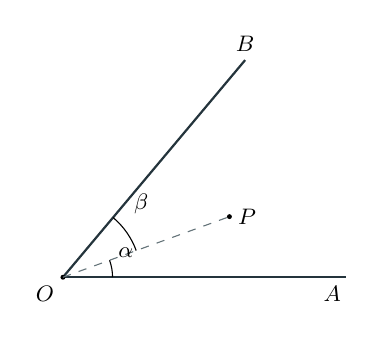
\begin{tikzpicture}[scale=.9,transform shape]
\draw[object] (0.00000,0.00000)--(4.00000,0.00000);\draw[object] (0.00000,0.00000)--(2.57115,3.06418);\fill (0.00000,0.00000) circle(.035);\node[below left] at (0.00000,0.00000) {$O$};\fill (2.34923,0.85505) circle(.035);\node[right] at (2.34923,0.85505) {$P$};\draw[guide] (0.00000,0.00000)--(2.34923,0.85505);\draw[thin] (.7,0) arc(0:20:.7);\draw[thin] (20:1.1) arc(20:50:1.1);\node[above] at (0.88633,0.15628) {$\alpha$};\node[above] at (1.10586,0.77433) {$\beta$};\node[below] at (3.80000,0.00000) {$A$};\node[above] at (2.57115,3.06418) {$B$};
\end{tikzpicture}
\figcaption{图光1.5\quad 镜间物点与两侧夹角}
\end{minipage}\end{center}

\Needspace{8\baselineskip}

\pdfbookmark[3]{题型定位}{q5-h0}

\subsection*{题型定位}

双平面镜的连续反射、像的圆周位置及观察范围。解图光1.5A先处理逐级反射和停止规则，B把真实两次反射展开成直线，C给出同一眼位的可见数，D处理整分角时同位像的合并。教学目标是能从具体光路决定计数，理解四个量各有不同含义：序列项数、不同位置数、最多同时可见数、指定眼位可见数。

\Needspace{8\baselineskip}

\pdfbookmark[3]{知识点}{q5-h1}

\subsection*{知识点}

\begin{itemize}
\item 反射映射$\mathcal R_A(\varphi)=-\varphi$、$\mathcal R_B(\varphi)=2\theta-\varphi$都保持半径。先写A、B两列前五项，再由两次反射相当于旋转$2\theta$归纳角度，既能确定位置，也能保留成像次序。
\item 解图光1.5A的奇数与偶数项分别沿相反方向进入两镜共同背面。非整数情形的末级严格不等式和整数等号必须分开；正常内部眼位的结果是$J_A=\lceil(\pi-\alpha)/\theta\rceil$、$J_B=\lceil(\pi-\beta)/\theta\rceil$，两列仍需去重。
\item 展开的直线穿每条正向镜面，等价于$|\varphi-\gamma|<\pi$。用开区间整数计数求每一眼位，再在有限个分界区间取最大。有限镜段还须将每个交点的正向距离与镜长比较；角度条件不能代替长度条件。
\end{itemize}

\Needspace{8\baselineskip}

\pdfbookmark[3]{物理图像}{q5-h2}

\subsection*{物理图像}

解图光1.5A中所有像与P共圆，灰扇区是共同背面；A奇数项每次顺时针推进$2\theta$，偶数项反向推进。解图光1.5B把P到E的两次反射实际画出：Y在镜B上，X在镜A上，展开后Y变成$Y'$，P变成U，四点共线。D的两组多边形含P在内共有$2m$个位置，两个末级标号落到一个点。C使两侧末级像的观察窗口直接可见：左端第五像与右端第五像不能在同一眼位出现。

\Needspace{8\baselineskip}

\pdfbookmark[3]{解题入口}{q5-h3}

\subsection*{解题入口}

从两镜垂直开始，让学生依次构造$A_1,B_1,A_2,B_2$，把两个二次像的位置坐标实际算出，确认它们是同一点，再问为何不是四像。随后改为60°，用两次反射的120°转动生成两组三点。最后再回到一般夹角：让学生先预测70°对称物点是4、5还是6像，再用解图光1.5C把三种答案各自对应的量说明白，避免先给一个不能覆盖各眼位的口诀。

\Needspace{8\baselineskip}

\Needspace{18\baselineskip}
\pdfbookmark[3]{标准解法}{q5-h4}

\subsection*{标准解法}


各次平面反射都保持到交棱的距离不变，故所有像点都在以$O$为心、$OP=\rho$为半径的圆上。取$OA$方向角为0，$OB$方向角为$\theta$，物点方向角为$\alpha$。镜面反射对方向角的作用为
\[
\mathcal R_A(\varphi)=-\varphi,\qquad
\mathcal R_B(\varphi)=2\theta-\varphi.
\]
从$A$先反射的一列依次为
\[
A_1:-\alpha,\quad A_2:2\theta+\alpha,\quad
A_3:-2\theta-\alpha,\quad A_4:4\theta+\alpha,\ldots;
\]
从$B$先反射的一列为
\[
B_1:2\theta-\alpha,\quad B_2:\alpha-2\theta,\quad
B_3:4\theta-\alpha,\quad B_4:\alpha-4\theta,\ldots.
\]
这些角应保留转动次序，最后再对$2\pi$取模；提前取模并任意继续反射，可能把背面也当作反射面。
\begin{center}\begin{minipage}{.98\linewidth}\centering
\begin{tikzpicture}[scale=.95,font=\small]
\fill[gray!12](0,0)--(180:2.3)arc(180:230:2.3)--cycle;
\draw[guide](0,0)circle(2.3);
\draw[object](0,0)--(3,0)node[right]{$A$};
\draw[object](0,0)--(50:3)node[above]{$B$};
\draw[guide](0,0)--(180:2.65);\draw[guide](0,0)--(230:2.65);
\node[above]at(180:2.65){$A'$};\node[below left]at(230:2.75){$B'$};
\draw[guide](0,0)--(18:2.3);
\draw(.65,0)arc(0:18:.65);\draw(18:1)arc(18:50:1);
\node at(9:.85){$\alpha$};\node at(34:1.2){$\beta$};
\node[below right]at(0,0){$O$};
\draw[guide,color=accent](-18:2.3)--(-118:2.3);
\draw[guide,color=warm](18:2.3)--(118:2.3)--(218:2.3);
\draw[->,color=accent](-18:1.6)arc(-18:-118:1.6);
\draw[->,color=warm](118:1.85)arc(118:218:1.85);
\node at(-68:1.35){$2\theta$};\node at(164:1.6){$2\theta$};
\fill[color=warm](2.18742999,0.71073909)circle(.035);\node at(2.49176807,0.80962453){$ P$};
\fill[color=accent](2.18742999,-0.71073909)circle(.035);\node at(2.49176807,-0.80962453){$ A_1$};
\fill[color=accent](-1.07978459,2.03077946)circle(.035);\node at(-1.23001549,2.31332269){$ A_2$};
\fill[color=accent](-1.07978459,-2.03077946)circle(.035);\node at(-1.23001549,-2.31332269){$ A_3$};
\fill[color=accent](-1.81242473,-1.41602139)circle(.035);\node at(-2.06458817,-1.61303307){$ A_4$};
\fill[color=muted](0.32009813,2.27761656)circle(.035);\node at(0.36463352,2.59450234){$ B_1$};
\fill[color=muted](0.32009813,-2.27761656)circle(.035);\node at(0.36463352,-2.59450234){$ B_2$};
\fill[color=muted](-2.29859890,-0.08026884)circle(.035);\node at(-2.61840397,-0.44){$ B_3$};
\node[align=left,anchor=west]at(3.7,.5){示例：$\theta=50^\circ,\ \alpha=18^\circ$\\奇数A项向顺时针推进\\偶数A项向逆时针推进\\每次跨过同奇偶项，角距增$2\theta$\\灰扇区为两镜共同背面\\末级$A_4,B_3$进入灰扇区\\反射序号须先保留，再作同位去重};
\end{tikzpicture}
\figcaption{解图光1.5A\quad 圆周上的两列像及同奇偶项的圆弧递推}
\end{minipage}\end{center}

\subsubsection*{从逐级圆弧推进到末级像}
解图光1.5A用$\theta=50^\circ,\alpha=18^\circ$显示同一圆上的两列像，灰区由两镜反向延长线$OA',OB'$围成。下列弧距按成像次序指定顺、逆时针，不是任取较小圆弧；暂取$OP=1$，弧距便等于相应圆心角。A列前五项逐次给
\[
\begin{aligned}
\widehat{PA_1}&=2\alpha,\\
\widehat{PA_2}&=\beta+\widehat{BA_2}
=\beta+\widehat{BA_1}=\beta+(\beta+2\alpha)=2\theta,\\
\widehat{PA_3}&=\alpha+\widehat{AA_3}
=\alpha+\widehat{AA_2}
=\alpha+\theta+\widehat{BA_1}
=\alpha+\theta+(\theta+\alpha)=2\alpha+2\theta,\\
\widehat{PA_4}&=\beta+\widehat{BA_4}
=\beta+\theta+\widehat{AA_2}\\
&=\beta+2\theta+\widehat{BA_1}
=\beta+2\theta+(\theta+\alpha)=4\theta,\\
\widehat{PA_5}&=\alpha+\widehat{AA_4}
=\alpha+\theta+\widehat{BA_3}
=\alpha+\theta+(3\theta+\alpha)=2\alpha+4\theta.
\end{aligned}
\]
这里相邻两次反射的镜面对称分别给$\widehat{BA_2}=\widehat{BA_1}$、$\widehat{AA_3}=\widehat{AA_2}$等关系。因而A列奇数项沿顺时针每隔$2\theta$推进，偶数项沿逆时针每隔$2\theta$推进，不能按脚标顺序把所有点都向同一方向累加。B列交换$\alpha,\beta$即可得到同样结构。

非退化位置中，若A列最后一项为奇数$2n+1$，进入灰区的判据为
\[
2\alpha+2n\theta>\pi-\beta
\ \Longrightarrow\ 2n\theta>\pi-\alpha-\theta
\ \Longrightarrow\ 2n+1>\frac{\pi-\alpha}{\theta}.
\]
若最后一项为偶数$2n$，则
\[
2n\theta>\pi-\alpha
\ \Longrightarrow\ 2n>\frac{\pi-\alpha}{\theta}.
\]
因此当$(\pi-\alpha)/\theta$不是整数时，A列末级脚标为刚好大于它的整数；B列应使用$(\pi-\beta)/\theta$。这是两列的停止规则，还不能把两项相加就作为不同像数。要进一步处理末项重合和观察方向；若比值恰为整数，必须把位于边界的光路单独核查。
\begin{center}\begin{minipage}{.97\linewidth}\centering
\begin{tikzpicture}[scale=.95,font=\small]
\draw[object](0,0)--(3,0)node[right]{$A$};
\draw[object](0,0)--(70:3)node[above]{$B$};
\node[below left]at(0,0){$O$};
\draw[motion](1.88404970,1.31922580)--(0.26498196,0.72803195)--(0.68430576,0.00000000)--(1.14681286,0.80300701);
\fill(1.88404970,1.31922580)circle(.03);\node[above right]at(1.88404970,1.31922580){$ P$};
\fill(1.14681286,0.80300701)circle(.03);\node[right]at(1.14681286,0.80300701){$ E$};
\fill(0.68430576,0.00000000)circle(.03);\node[below]at(0.68430576,0.00000000){$ X$};
\fill(0.26498196,0.72803195)circle(.03);\node[above left]at(0.26498196,0.72803195){$ Y$};
\node[align=center]at(1.4,-2.8){折回的真实光路$P\to Y\to X\to E$\\两镜反射点均在正向镜面};
\begin{scope}[xshift=6.7cm]
\draw[guide](0,0)--(3,0)node[right]{$0$};
\draw[guide](0,0)--(-70:3)node[below]{$-\theta$};
\draw[guide](0,0)--(-140:2.6)node[left]{$-2\theta$};
\node[above left]at(0,0){$O$};
\draw[motion](-0.59528380,-2.22162940)--(1.14681286,0.80300701);
\fill(-0.59528380,-2.22162940)circle(.03);\node[below right]at(-0.59528380,-2.22162940){$ U$};
\fill(1.14681286,0.80300701)circle(.03);\node[above]at(1.14681286,0.80300701){$ E$};
\fill(0.68430576,0.00000000)circle(.03);\node[right]at(0.79,0){$ X$};
\fill(0.26498196,-0.72803195)circle(.03);\node[below right]at(0.26498196,-0.72803195){$ Y'$};
\node[align=left,anchor=west]at(3.35,-.8){$\theta=70^\circ,\alpha=\gamma=35^\circ$\\$U$为$B_2$的展开副本\\$\varphi_U=-105^\circ$\\$|\varphi_U-\gamma|=140^\circ<180^\circ$\\两交点顺序：$E,X,Y',U$};
\end{scope}
\end{tikzpicture}
\figcaption{解图光1.5B　左图是两次实际反射，右图是对应展开直线。X与Y为真实镜面交点，展开点U折回后就是物点P。}
\end{minipage}\end{center}

解图光1.5B中，先让$E$看到经镜A反射的最后一段，再将镜B的反射展开，光路成为$U,Y',X,E$的一条直线。$Y'$关于OA对称后落回镜B上的Y。两次对称保持交角，所以展开线与镜面交点的位置和先后顺序都必须保留；圆周上有一个候选像点，本身并不保证该眼位有反射光到达。

\subsubsection*{一般夹角下怎样计数}
解图光1.5B将镜间扇区连续展开。第$j$个展开扇区中的物点方向角为
\[
\varphi_{2k}=2k\theta+\alpha,\qquad
\varphi_{2k-1}=2k\theta-\alpha,\qquad k\in\mathbb Z.
\]
设观察者方向角为$0<\gamma<\theta$。把反射光路展开成直线后，它从观察者到对应物点副本时必须依次穿过正向镜面，不能绕过交点$O$的背后。等价条件为
\[
\gamma-\pi<\varphi_j<\gamma+\pi.
\]
证明可从直线段的极角变化看出：不通过$O$的线段，其连续极角变化严格小于$\pi$；当两端角差小于$\pi$时，沿途各展开镜面的交点均在正向半径上。等号是经过交棱或掠射的退化光路，不计入通常可见像。
定义整数计数函数
\[
C(a,b)=\#\{k\in\mathbb Z:a<k<b\}
=\lceil b\rceil-\lfloor a\rfloor-1.
\]
则一个确定观察方向可见的像数为
\[
\begin{split}
N(\gamma)={}&
C\!\left(\frac{\gamma-\pi-\alpha}{2\theta},
         \frac{\gamma+\pi-\alpha}{2\theta}\right)\\
&+C\!\left(\frac{\gamma-\pi+\alpha}{2\theta},
          \frac{\gamma+\pi+\alpha}{2\theta}\right)-1.
\end{split}
\]
最后减1排除实际物点。因开区间宽度恰为$2\pi$，不会把相差$2\pi$的同一位置重复算入。一般问题的明确答案是
\[
\boxed{N_{\max}=\max_{0<\gamma<\theta}N(\gamma)}.
\]
还可把逐级停止规则写成含边界的明确式。A列某一级的有向展开角，奇数为$-(j-1)\theta-\alpha$，偶数为$j\theta+\alpha$。存在某个镜间眼位的充要条件是其有向角落在$(-\pi,\pi+\theta)$；两种奇偶都化为
\[
j<1+\frac{\pi-\alpha}{\theta}.
\]
故允许的最大正整数脚标以及B列的对应脚标为
\[
J_A=\left\lceil\frac{\pi-\alpha}{\theta}\right\rceil,\qquad
J_B=\left\lceil\frac{\pi-\beta}{\theta}\right\rceil.
\]
在非整数情形，这与上面的“刚好大于”相同；恰为整数时，不能再额外加1，否则会将只能经交点O到达的退化项列入。列完$A_1,\ldots,A_{J_A}$和$B_1,\ldots,B_{J_B}$后，还须对$2\pi$取模并合并同位点，才得到从不同眼位能够看到的全部像的位置集合。

只需检查有限个区间：$N$只在$\gamma=2k\theta\pm\alpha\pm\pi$落入$(0,\theta)$时改变，列出这些有限分界点，在相邻区间各取一点即可得到最大值与可见范围。把两列在不同观察方向能产生的末级像简单相加，可能高估同一位置的可见数。
\begin{center}\begin{minipage}{.97\linewidth}\centering
\begin{tikzpicture}[x=.105cm,y=1.0cm,font=\small]
\draw[axis](-3,3.4)--(80,3.4)node[right]{$\gamma/{}^\circ$};
\draw[axis](0,3.4)--(0,5.9)node[above]{$N(\gamma)$};
\draw[guide](5,3.4)--(5,5);\draw[guide](65,3.4)--(65,5);
\draw[guide](70,3.4)--(70,5);
\draw[traj](0,5)--(5,5);\draw[traj](5,4)--(65,4);\draw[traj](65,5)--(70,5);
\foreach \a/\b in{0/5,5/5,65/5,70/5}{\draw[color=accent,fill=white](\a,\b)circle(2.2pt);}
\fill[color=accent](5,4)circle(1.3pt);\fill[color=accent](65,4)circle(1.3pt);
\node[left]at(0,4){4};\node[left]at(0,5){5};
\foreach \a in{5,35,65,70}{\node[below]at(\a,3.4){\a};}
\node[align=left,anchor=west]at(84,4.7){$\theta=70^\circ,\alpha=35^\circ$\\$A_3$只在$0<\gamma<5^\circ$可见\\$B_3$只在$65^\circ<\gamma<70^\circ$可见\\两末级像不能同时进入同一眼位\\不同位置共6像，最多同时见5像};
\end{tikzpicture}
\figcaption{解图光1.5C　固定物点时的可见数随眼位变化。空心点排除该端点，实心点计入；两侧各自可见的末级像不能合成同一眼位的结果。}
\end{minipage}\end{center}

解图光1.5C把一般计数实际算一遍。取$\theta=70^\circ,\alpha=\beta=35^\circ$，两列到第3级停止：
\[
\begin{array}{c|ccc}
 &1&2&3\\ \hline
A_j&-35^\circ&175^\circ&-175^\circ\\
B_j&105^\circ&-105^\circ&245^\circ
\end{array}
\]
六个模$360^\circ$位置各不相同。前四个较低级像在所有$0<\gamma<70^\circ$眼位都能看到；末项$A_3$需$\gamma<5^\circ$，末项$B_3$需$\gamma>65^\circ$，这两个条件不能同时成立。因此
\[
N(\gamma)=
\begin{cases}
5,&0<\gamma<5^\circ\ \text{或}\ 65^\circ<\gamma<70^\circ,\\
4,&5^\circ\le\gamma\le65^\circ.
\end{cases}
\]
在$5^\circ$或$65^\circ$处，那一级展开线恰穿O，应按开区间计数。图中的平台由实际光路的存在条件得到，不能用“形成6像”代替“最多同时见5像”。

\subsubsection*{本题三个整分角}
当$\theta=\pi/m$时，$2m$个展开扇区闭合。不同像的位置可用
\[
\varphi=2k\theta+\alpha,\quad 2k\theta-\alpha,
\qquad k=0,1,\ldots,m-1
\]
表示，再从中去掉$\varphi=\alpha$的物点。由于$0<\alpha<\theta$，两组在圆周上各$m$点且互不重合；有
\[
\boxed{N=2m-1}.
\]
这里$N$指不同像的总数，也是在一般眼位能同时看到的最大数。解图光1.5D给出三种分布；镜角及像数分别为
\[
\theta=\pi/5:\ 9,\qquad
\theta=\pi/3:\ 5,\qquad
\theta=\pi/2:\ 3.
\]
\begin{center}\begin{minipage}{.98\linewidth}\centering
\begin{tikzpicture}[scale=.95,font=\small]
\begin{scope}[xshift=0.0cm]
\draw[guide](0,0)circle(1.5);\draw[object](0,0)--(1.8,0);\draw[object](0,0)--(36.00000000:1.8);
\draw[thin,color=warm](1.46179031,0.33640614)--(0.13177679,1.49420041)--(-1.38034777,0.58706050)--(-0.98487863,-1.13137707)--(0.77165930,-1.28628998)--cycle;
\draw[thin,color=accent](1.46179031,-0.33640614)--(0.77165930,1.28628998)--(-0.98487863,1.13137707)--(-1.38034777,-0.58706050)--(0.13177679,-1.49420041)--cycle;
\fill(0.77165930,1.28628998)circle(.025);\node[font=\scriptsize]at(0.98257951,1.63787591){$ B_1$};
\fill(0.13177679,1.49420041)circle(.025);\node[font=\scriptsize]at(0.16779579,1.90261519){$ A_2$};
\fill(-0.98487863,1.13137707)circle(.025);\node[font=\scriptsize]at(-1.25407879,1.44062014){$ B_3$};
\fill(-1.38034777,0.58706050)circle(.025);\node[font=\scriptsize]at(-1.75764283,0.74752370){$ A_4$};
\fill(-1.38034777,-0.58706050)circle(.025);\node[font=\scriptsize,anchor=east]at(-1.75764283,-0.74752370){$ A_5=B_5$};
\fill(-0.98487863,-1.13137707)circle(.025);\node[font=\scriptsize]at(-1.25407879,-1.44062014){$ B_4$};
\fill(0.13177679,-1.49420041)circle(.025);\node[font=\scriptsize]at(0.16779579,-1.90261519){$ A_3$};
\fill(0.77165930,-1.28628998)circle(.025);\node[font=\scriptsize]at(0.98257951,-1.63787591){$ B_2$};
\fill(1.46179031,-0.33640614)circle(.025);\node[font=\scriptsize]at(1.86134633,-0.42835715){$ A_1$};
\draw[color=warm,thick](1.40679031,0.28140614)--(1.51679031,0.39140614);
\fill[color=warm](1.46179031,0.33640614)circle(.035);\node[font=\scriptsize]at(1.86134633,0.42835715){$P$};
\node at(0,-2.45){$\theta=\pi/5,\quad 9\text{个不同像}$};
\end{scope}
\begin{scope}[xshift=4.5cm]
\draw[guide](0,0)circle(1.5);\draw[object](0,0)--(1.8,0);\draw[object](0,0)--(60.00000000:1.8);
\draw[thin,color=warm](1.39466473,0.55218683)--(-1.17554019,0.93172167)--(-0.21912454,-1.48390850)--cycle;
\draw[thin,color=accent](1.39466473,-0.55218683)--(-0.21912454,1.48390850)--(-1.17554019,-0.93172167)--cycle;
\fill(-0.21912454,1.48390850)circle(.025);\node[font=\scriptsize]at(-0.27901858,1.88951016){$ B_1$};
\fill(-1.17554019,0.93172167)circle(.025);\node[font=\scriptsize]at(-1.49685450,1.18639226){$ A_2$};
\fill(-1.17554019,-0.93172167)circle(.025);\node[font=\scriptsize,anchor=east]at(-1.49685450,-1.18639226){$ A_3=B_3$};
\fill(-0.21912454,-1.48390850)circle(.025);\node[font=\scriptsize]at(-0.27901858,-1.88951016){$ B_2$};
\fill(1.39466473,-0.55218683)circle(.025);\node[font=\scriptsize]at(1.77587309,-0.70311790){$ A_1$};
\draw[color=warm,thick](1.33966473,0.49718683)--(1.44966473,0.60718683);
\fill[color=warm](1.39466473,0.55218683)circle(.035);\node[font=\scriptsize]at(1.77587309,0.70311790){$P$};
\node at(0,-2.45){$\theta=\pi/3,\quad 5\text{个不同像}$};
\end{scope}
\begin{scope}[xshift=9.0cm]
\draw[guide](0,0)circle(1.5);\draw[object](0,0)--(1.8,0);\draw[object](0,0)--(90.00000000:1.8);
\draw[thin,color=warm](1.26649189,0.80374019)--(-1.26649189,-0.80374019);
\draw[thin,color=accent](1.26649189,-0.80374019)--(-1.26649189,0.80374019);
\fill(-1.26649189,0.80374019)circle(.025);\node[font=\scriptsize]at(-1.61266634,1.02342918){$ B_1$};
\fill(-1.26649189,-0.80374019)circle(.025);\node[font=\scriptsize,anchor=east]at(-1.61266634,-1.02342918){$ A_2=B_2$};
\fill(1.26649189,-0.80374019)circle(.025);\node[font=\scriptsize]at(1.61266634,-1.02342918){$ A_1$};
\draw[color=warm,thick](1.21149189,0.74874019)--(1.32149189,0.85874019);
\fill[color=warm](1.26649189,0.80374019)circle(.035);\node[font=\scriptsize]at(1.61266634,1.02342918){$P$};
\node at(0,-2.45){$\theta=\pi/2,\quad 3\text{个不同像}$};
\end{scope}
\end{tikzpicture}
\figcaption{解图光1.5D\quad 三个整分角分别形成9、5、3个像}
\end{minipage}\end{center}

把圆周位置与逐级序列对应，才能看清为什么合并后少一项。当$\theta=\pi/m$，$J_A=J_B=m$，两列共有$2m$个记录；最后的$A_m,B_m$落在同一位置，只能保留一个。等价地，加上P后的$2m$个不同圆周点分成两组：
\[
\{2k\theta-\alpha\}_{k=0}^{m-1},\qquad
\{2k\theta+\alpha\}_{k=0}^{m-1}.
\]
同组相邻点角距为$2\pi/m$，分别形成正m边形；第二组有一个点是P。两组若有同位点，必有$2\alpha=2l\theta\pmod{2\pi}$，这与$0<\alpha<\theta$矛盾，所以不能再删掉任意一组中的其他点。

解图光1.5D左图中，奇数项多边形可依次写成
\[
A_1,A_3,A_5(=B_5),B_3,B_1,A_1,
\]
另一五边形为$P,A_2,A_4,B_4,B_2,P$。十个不同顶点里一个是P，故有9像。中图为三角形$A_1,A_3(=B_3),B_1$与$P,A_2,B_2$，六点扣掉P后为5像。右图$m=2$时，两组多边形退化为线段$A_1B_1$与$PA_2$；$A_2=B_2$，故有3像。图上不同颜色表示这两组圆周点，P另作标记。

还要说明“各眼位都能看见”的例外。若一个像的方向恰为$\gamma+\pi$，眼睛与其展开副本的连线必穿O，正常反射光路不存在。对于$\theta=\pi/m$，
\[
\gamma_*=
\begin{cases}
\alpha,&m\text{为偶数},\\
\theta-\alpha=\beta,&m\text{为奇数},
\end{cases}
\qquad
N(\gamma_*)=2m-2.
\]
离开这个孤立方向后，$N(\gamma)=2m-1$。因此三问的不同像总数、最多可见数均为9、5、3，但在相应退化眼位严格计数时分别只能见8、4、2个；这并不改变已形成的像的位置集合。这个例外针对理想点物和眼睛，实际有限物点、有限瞳孔可由邻近光线看到轮廓，不能拿它取消几何判别。

各像的笛卡儿坐标为$(\rho\cos\varphi,\rho\sin\varphi)$，因此上述角度列表已完整确定位置。对于$\pi/2$，三像尤其直观：方向角为$-\alpha,\pi-\alpha,\pi+\alpha$，其中最后一个像可经两条反射次序得到，但只能计一次。

\subsubsection*{有限镜长时怎样落实可见性}
解图光1.5B还能直接用于有限镜长：设展开线为$\boldsymbol z(t)=\boldsymbol e+t\boldsymbol v$，$\boldsymbol v=\boldsymbol u-\boldsymbol e$，某镜面展开后为方向单位矢量$\boldsymbol d_j$上的线段。定义平面有向积$[\boldsymbol a,\boldsymbol b]=a_xb_y-a_yb_x$，由$\boldsymbol e+t_j\boldsymbol v=s_j\boldsymbol d_j$得
\[
t_j=-\frac{[\boldsymbol e,\boldsymbol d_j]}{[\boldsymbol v,\boldsymbol d_j]},
\qquad
s_j=\frac{[\boldsymbol e,\boldsymbol v]}{[\boldsymbol d_j,\boldsymbol v]}.
\]
若镜段从O延伸到长度$L_j$，每个交点都须满足$0<t_j<1$、$0<s_j<L_j$，并按实际反射先后排列。分母为0时是平行或重合退化情形，另行判断，不能直接除。无限镜面的角窗口只保证正向交点存在；镜段不足、遮挡或实际开口还可能删去光路。图中射线方向为P到E，按观察者反追时顺序是E、X、Y、P，两种叙述须互相对应。



\Needspace{8\baselineskip}

\pdfbookmark[3]{关键洞察}{q5-h5}

\subsection*{关键洞察}

一个圆周方向只有候选位置的含义。解图光1.5B中还必须有正向、有序的镜面交点，才能折回为到达E的真实光路。展开窗口长度为$2\pi$，其端点随眼位移动；这使同一个物点的可见数出现C图中的跳变。整分角时两组正多边形闭合，位置数固定为$2m-1$，但某一像与眼位径向相背时，展开线恰过O，严格可见数仍少1。位置重合与光路退化是两种不同的删项原因。

\Needspace{8\baselineskip}

\pdfbookmark[3]{易错点}{q5-h6}

\subsection*{易错点}

\begin{itemize}
\item 将A列脚标顺序当成圆周上的同向顺序。应分别检查A奇数项和偶数项，利用A图的两支$2\theta$步进，才不会将末级位置算错。
\item 把$\lfloor x\rfloor+1$用于整数等号。先由内部眼位的严格不等式$j<1+x$求允许的最大整数；当$x$恰为整数，只能取j=x，不能再加1。120°且物点在角平分线的例子可直接检出此错。
\item 两列脚标不同便重复计数。60°的$A_3=B_3$、90°的$A_2=B_2$都应在D图中合成一个位置，再排除实物P。
\item 将70°时可形成6像说成同时可见6像，或把9、5、3说成无例外适用于所有点眼位。应先固定同一个$\gamma$，检查每个展开角是否严格在窗口内；过O的等号项不能保留。
\item 用无限镜面结论保证有限镜段可见。B图的交点必须逐个核查$0<s_j<L_j$；只要有一个超出镜长，整条反射路径就失效。
\end{itemize}

\Needspace{8\baselineskip}

\pdfbookmark[3]{课堂讲解建议}{q5-h7}

\subsection*{课堂讲解建议}

先用解图光1.5B做一次正向与反向追迹：学生依次指出P、Y、X、E，再反向读E、X、Y、P；展开后对应E、X、$Y'$、U。追问“U在圆上，为什么还要检查直线？”要求回答每条镜面的交点要在正向半镜上。随后由A图完整写出五项弧距，归纳两支步进，保留奇数和偶数末级的两段不等式，不用一句“按规律”跳过。

计数训练使用C图：中央$\gamma=35^\circ$见4像，靠近镜A的$\gamma=2^\circ$见5像，靠近镜B的$\gamma=68^\circ$也见5像，但两端多出的像不是同一个。让学生解出5°和65°两个界点，并说明等号为何计4。最后用D图核对9、5、3个位置，再设60°镜角、20°物角、40°眼位，检验过O的220°像为何暂时看不到。作业答案必须列窗口、排除项及同位合并，只有最后一个整数不算完成推导。

\Needspace{8\baselineskip}

\Needspace{18\baselineskip}
\pdfbookmark[3]{变式训练}{q5-h8}

\subsection*{变式训练}

\begin{enumerate}
\Needspace{7\baselineskip}
\item 若$\theta=\pi/4$，取$k=0,1,2,3$的$2k\theta\pm\alpha$，两组各四个点，分别是相隔90°的正方形；$0<\alpha<45^\circ$保证两组不重合。共8个圆周点，删去实物得7像，两列末级$A_4=B_4$只计一次。最多可见数也为7；在$\gamma=\alpha$处，方向为$\alpha+180^\circ$的一像需要过O的光路，严格可见数降为6。

变图光1.5V1中，八个标记点由 $2k\theta\pm20^\circ$ 计算；$P$ 属于其中一组，删去它后为七像，退化眼位 $\gamma=20^\circ$ 另排除过 $O$ 的路径。

\begin{center}\begin{minipage}{.97\linewidth}\centering
\begin{tikzpicture}[scale=1.2,font=\small]
\draw[guide](0,0)circle(1.6);\draw[object](0.000000000000,0.000000000000)--(2.000000000000,0.000000000000);
\draw[object](0.000000000000,0.000000000000)--(1.414213562373,1.414213562373);
\fill(1.503508193257,0.547232229321) circle(1.2pt);\node[above]at(1.503508193257,0.547232229321){$P$};
\fill(0.547232229321,1.503508193257) circle(1.2pt);\node[above]at(0.547232229321,1.503508193257){$70^\circ$};
\fill(-0.547232229321,1.503508193257) circle(1.2pt);\node[above]at(-0.547232229321,1.503508193257){$110^\circ$};
\fill(-1.503508193257,0.547232229321) circle(1.2pt);\node[above left]at(-1.503508193257,0.547232229321){$160^\circ$};
\fill(-1.503508193257,-0.547232229321) circle(1.2pt);\node[below left]at(-1.503508193257,-0.547232229321){$200^\circ$};
\fill(-0.547232229321,-1.503508193257) circle(1.2pt);\node[below]at(-0.547232229321,-1.503508193257){$250^\circ$};
\fill(0.547232229321,-1.503508193257) circle(1.2pt);\node[below]at(0.547232229321,-1.503508193257){$290^\circ$};
\fill(1.503508193257,-0.547232229321) circle(1.2pt);\node[below right]at(1.503508193257,-0.547232229321){$340^\circ$};
\node[anchor=north,align=center]at(0.000000000000,-2.200000000000){$\alpha=20^\circ$；八个位置中一个为实物，故有七个不同像。};
\end{tikzpicture}
\figcaption{变图光1.5V1\quad 四十五度双镜的两组圆周位置}
\end{minipage}\end{center}

\Needspace{7\baselineskip}
\item 取$\theta=120^\circ,\alpha=60^\circ$。窗口为$(\gamma-180^\circ,\gamma+180^\circ)$，两个第一像方向$-60^\circ,180^\circ$对所有$0<\gamma<120^\circ$都满足严格条件；其余候选展开项需要边界眼位而被排除。故最多和指定内部眼位都只有2像，不能不分物点位置便套$360^\circ/\theta$。还应解释两列停止式此时为整数等号，为什么不能给各列再加一级。

变图光1.5V2中，水平段表示 $0<\gamma<120^\circ$ 内始终为两像；左右空心端点排除镜面边界眼位。

\begin{center}\begin{minipage}{.97\linewidth}\centering
\begin{tikzpicture}[x=.055cm,y=.8cm,font=\small]
\draw[axis](0.000000000000,0.000000000000)--(130.000000000000,0.000000000000);
\draw[axis](0.000000000000,0.000000000000)--(0.000000000000,3.200000000000);
\node[right]at(130.000000000000,0.000000000000){$\gamma/{}^\circ$};\node[above]at(0.000000000000,3.200000000000){$N(\gamma)$};
\draw[thin,color=muted](-2,1)--(0,1);\node[left]at(-2,1){$1$};
\draw[thin,color=muted](-2,2)--(0,2);\node[left]at(-2,2){$2$};
\draw[thin,color=muted](-2,3)--(0,3);\node[left]at(-2,3){$3$};
\node[below left]at(0,0){$0$};\node[below]at(120,0){$120^\circ$};
\draw[traj](0.000000000000,2.000000000000)--(120.000000000000,2.000000000000);
\draw[color=accent,fill=white](0.000000000000,2.000000000000)circle(2pt);
\draw[color=accent,fill=white](120.000000000000,2.000000000000)circle(2pt);
\node[anchor=north,align=center]at(60.000000000000,-0.500000000000){$\theta=120^\circ,\alpha=60^\circ$；两像方向为 $-60^\circ,180^\circ$。};
\end{tikzpicture}
\figcaption{变图光1.5V2\quad 对称物点在一百二十度双镜间始终只见两像}
\end{minipage}\end{center}

\Needspace{7\baselineskip}
\item 取$\theta=120^\circ,\alpha=30^\circ$，则$\beta=90^\circ$，$J_A=2$、$J_B=1$。三个不同像的方向为$-30^\circ,210^\circ,270^\circ$。其中$-30^\circ$像在全部内部眼位可见，$210^\circ$像还要求$\gamma>30^\circ$（等号不计）；第三个要求$270^\circ-\gamma<180^\circ$，即$\gamma>90^\circ$；90°等号不计。中央60°眼位只见前两像，而90°到120°之间见3像；同一镜角改变物点位置后，结果与上一变式不同。

变图光1.5V3中，$\gamma=90^\circ$ 的实心点位于 $N=2$；$30^\circ$ 处的实心点位于 $N=1$。两处上方空心点都排除过 $O$ 的退化路径，所以三段依次为一、二、三像。

\begin{center}\begin{minipage}{.97\linewidth}\centering
\begin{tikzpicture}[x=.055cm,y=.8cm,font=\small]
\draw[axis](0,0)--(130,0)node[right]{$\gamma/{}^\circ$};
\draw[axis](0,0)--(0,4.1)node[above]{$N(\gamma)$};
\draw[thin,color=muted](-2,1)--(0,1);\node[left]at(-2,1){$1$};
\draw[thin,color=muted](-2,2)--(0,2);\node[left]at(-2,2){$2$};
\draw[thin,color=muted](-2,3)--(0,3);\node[left]at(-2,3){$3$};
\node[below left]at(0,0){$0$};\node[below]at(120,0){$120^\circ$};
\draw[traj](0,1)--(30,1);\draw[traj](30,2)--(90,2);\draw[traj](90,3)--(120,3);
\draw[guide](30,0)--(30,2);\draw[guide](90,0)--(90,3);
\fill(30,1)circle(1.2pt);\fill(90,2)circle(1.2pt);
\foreach \x/\y in{0/1,30/2,90/3,120/3}{\draw[color=accent,fill=white](\x,\y)circle(2pt);}
\node[below]at(30,0){$30^\circ$};\node[below]at(90,0){$90^\circ$};
\node[anchor=north,align=center]at(60,-.65){$\theta=120^\circ,\alpha=30^\circ$；两个跳点的高侧都是空心点。纵轴1、2、3直接给出各段像数。};
\end{tikzpicture}
\figcaption{变图光1.5V3\quad 非对称物点的第三像只进入部分眼位}
\end{minipage}\end{center}

\Needspace{7\baselineskip}
\item 镜面改为有限长度。沿解图光1.5B的展开直线先求每条镜面的$t_j,s_j$，核查交点顺序及$0<s_j<L_j$。例如图示$\theta=70^\circ,\alpha=\gamma=35^\circ$、$OP=2.3$、$OE=1.4$时，两交点距O分别约为0.6843与0.7748；若两镜都长0.62，这条二次反射路径失效，长0.85则能容纳两交点。数值须由交点方程算出，不能只因像点在角窗口里就判可见；其他光路还要各自检查。

变图光1.5V4中，$P\to Y\to X\to E$ 满足两次反射；$X,Y$ 均在暖色短镜段之外，而在加长到 $0.85$ 的镜段内。

\begin{center}\begin{minipage}{.97\linewidth}\centering
\begin{tikzpicture}[scale=1.75,font=\small]
\draw[very thick,color=warm](0.000000000000,0.000000000000)--(0.620000000000,0.000000000000);
\draw[very thick,color=accent](0.620000000000,0.000000000000)--(0.850000000000,0.000000000000);
\draw[guide](0.850000000000,0.000000000000)--(1.350000000000,0.000000000000);
\draw[very thick,color=warm](0.000000000000,0.000000000000)--(0.212052488862,0.582609424887);
\draw[very thick,color=accent](0.212052488862,0.582609424887)--(0.290717121827,0.798738727668);
\draw[guide](0.290717121827,0.798738727668)--(0.461727193490,1.268585038061);
\draw[motion](1.884049701865,1.319225803607)--(0.264981957834,0.728031945711);
\draw[motion](0.264981957834,0.728031945711)--(0.684305755039,0.000000000000);
\draw[motion](0.684305755039,0.000000000000)--(1.146812862005,0.803007010891);
\fill(1.884049701865,1.319225803607) circle(1.2pt);\node[above right]at(1.884049701865,1.319225803607){$P$};
\fill(1.146812862005,0.803007010891) circle(1.2pt);\node[right]at(1.146812862005,0.803007010891){$E$};
\fill(0.684305755039,0.000000000000) circle(1.2pt);\node[below]at(0.684305755039,0.000000000000){$X$};
\fill(0.264981957834,0.728031945711) circle(1.2pt);\node[left]at(0.264981957834,0.728031945711){$Y$};
\node[anchor=north,align=center]at(1.000000000000,-0.500000000000){暖色镜段长 $0.62$；加上青色段后长 $0.85$。\\$OX=0.6843, OY=0.7748$，须逐段检查镜长。};
\end{tikzpicture}
\figcaption{变图光1.5V4\quad 有限镜长决定这条两次反射光路是否存在}
\end{minipage}\end{center}


\Needspace{7\baselineskip}
\item 保持$\theta=70^\circ,\alpha=35^\circ$，移动眼位。先按解图光1.5C列四个始终可见像，再分别解$|\gamma+175^\circ|<180^\circ$和$|\gamma-245^\circ|<180^\circ$，得到$\gamma<5^\circ$或$\gamma>65^\circ$。说明两端的第五像属于不同位置，六个可形成像并不在同一眼位同时出现；端点恰过O时只计4个。

变图光1.5V5中，$5^\circ,65^\circ$ 的实心点都位于 $N=4$；左端高段来自 $A_3$，右端高段来自 $B_3$；两段对应的眼位不相交。

\begin{center}\begin{minipage}{.97\linewidth}\centering
\begin{tikzpicture}[x=.085cm,y=.9cm,font=\small]
\draw[axis](0.000000000000,3.300000000000)--(80.000000000000,3.300000000000);
\draw[axis](0.000000000000,3.300000000000)--(0.000000000000,5.800000000000);
\node[right]at(80.000000000000,3.300000000000){$\gamma/{}^\circ$};\node[above]at(0.000000000000,5.800000000000){$N(\gamma)$};
\draw[thin,color=muted](-1.5,4)--(0,4);\node[left]at(-1.5,4){$4$};
\draw[thin,color=muted](-1.5,5)--(0,5);\node[left]at(-1.5,5){$5$};
\node[below left]at(0,3.3){$0$};
\draw[traj](0.000000000000,5.000000000000)--(5.000000000000,5.000000000000);
\draw[traj](5.000000000000,4.000000000000)--(65.000000000000,4.000000000000);
\draw[traj](65.000000000000,5.000000000000)--(70.000000000000,5.000000000000);
\draw[color=accent,fill=white](0.000000000000,5.000000000000)circle(2pt);
\draw[color=accent,fill=white](5.000000000000,5.000000000000)circle(2pt);
\draw[color=accent,fill=white](65.000000000000,5.000000000000)circle(2pt);
\draw[color=accent,fill=white](70.000000000000,5.000000000000)circle(2pt);
\fill(5.000000000000,4.000000000000) circle(1.2pt);\node[below]at(5.000000000000,4.000000000000){};
\fill(65.000000000000,4.000000000000) circle(1.2pt);\node[below]at(65.000000000000,4.000000000000){};
\node[below]at(5.000000000000,3.300000000000){$5$};
\node[below]at(65.000000000000,3.300000000000){$65$};
\draw[thin,color=muted](70,3.3)--(74,3.0)node[right]{$70$};
\node[anchor=north,align=center]at(35.000000000000,2.650000000000){$\theta=70^\circ,\alpha=35^\circ$；两端第五像的空间位置不同。};
\end{tikzpicture}
\figcaption{变图光1.5V5\quad 移动眼位时两个末级像不能同时进入视野}
\end{minipage}\end{center}

\Needspace{7\baselineskip}
\item 取$\theta=60^\circ$且$\alpha=20^\circ$。列两组三点$2k60^\circ\pm20^\circ$，得到像的五个方向$-20^\circ,100^\circ,140^\circ,220^\circ,260^\circ$。当$\gamma=40^\circ=\beta$时，220°像恰与眼睛相背，展开线穿O，严格可见数为4；改成$\gamma=39^\circ$或41°便恢复5。要求学生把形成数、最多可见数和指定眼位数分别写出。

变图光1.5V6中，$E$ 与 $220^\circ$ 副本的连线穿过 $O$；该位置仍属于五像集合，但不产生这条正常反射光路。

\begin{center}\begin{minipage}{.97\linewidth}\centering
\begin{tikzpicture}[scale=1.1,font=\small]
\draw[guide](0,0)circle(1.6);\draw[object](0.000000000000,0.000000000000)--(2.000000000000,0.000000000000);
\draw[object](0.000000000000,0.000000000000)--(1.000000000000,1.732050807569);
\fill(1.503508193257,0.547232229321) circle(1.2pt);\node[above]at(1.503508193257,0.547232229321){$P$};
\fill(1.503508193257,-0.547232229321) circle(1.2pt);\node[below right]at(1.503508193257,-0.547232229321){$-20^\circ$};
\fill(-0.277837084267,1.575692404820) circle(1.2pt);\node[above]at(-0.277837084267,1.575692404820){$100^\circ$};
\fill(-1.225671108990,1.028460175498) circle(1.2pt);\node[above left]at(-1.225671108990,1.028460175498){$140^\circ$};
\fill(-1.225671108990,-1.028460175498) circle(1.2pt);\node[below left]at(-1.225671108990,-1.028460175498){$220^\circ$};
\fill(-0.277837084267,-1.575692404820) circle(1.2pt);\node[below]at(-0.277837084267,-1.575692404820){$260^\circ$};
\fill(0.536231110183,0.449951326781) circle(1.2pt);\node[below right]at(0.536231110183,0.449951326781){$E$};
\draw[guide](0.536231110183,0.449951326781)--(-1.225671108990,-1.028460175498);
\fill(0.000000000000,0.000000000000) circle(1.2pt);\node[below right]at(0.000000000000,0.000000000000){$O$};
\node[anchor=north,align=center]at(0.000000000000,-2.300000000000){$\gamma=40^\circ$ 时 $E,O,220^\circ$ 副本共线，严格可见数降为四。};
\end{tikzpicture}
\figcaption{变图光1.5V6\quad 六十度双镜的孤立退化眼位}
\end{minipage}\end{center}

\Needspace{7\baselineskip}
\item 考查末级取整等号：取$\theta=120^\circ,\alpha=\beta=60^\circ$。此时$(180^\circ-\alpha)/\theta=1$，故$J_A=J_B=1$。若机械取“严格大于的最小整数”，会虚增两项；这两项需要$\gamma=0$或120°的边界眼位，镜间开区间中不存在相应正常光路。两第一像方向为$-60^\circ,180^\circ$，所有内部眼位都只能见2像。

变图光1.5V7中，实心点表示允许的第一反射，空心点标出严格不等式排除的第二级；两列都只有 $j=1$。

\begin{center}\begin{minipage}{.97\linewidth}\centering
\begin{tikzpicture}[x=2cm,y=1.5cm,font=\small]
\draw[axis](0.500000000000,0.000000000000)--(3.500000000000,0.000000000000);
\draw[axis](0.500000000000,0.000000000000)--(0.500000000000,1.100000000000);
\node[right]at(3.500000000000,0.000000000000){$j$};\node[above]at(0.500000000000,1.100000000000){末级判据};
\fill(1.000000000000,0.000000000000) circle(1.2pt);\node[above]at(1.000000000000,0.000000000000){$j=1$};
\draw[color=warm,fill=white](2,0)circle(2.5pt);\node[above]at(2,.3){$j=2$ 等号};\node[anchor=north,align=center]at(2.000000000000,-0.450000000000){$j<1+(180^\circ-60^\circ)/120^\circ=2$。\\正整数只剩 $j=1$；$j=2$ 对应边界眼位，不能保留。};
\end{tikzpicture}
\figcaption{变图光1.5V7\quad 末级停止不等式的整数等号必须排除}
\end{minipage}\end{center}

\Needspace{7\baselineskip}
\item 反射系数为$q$且各反射光束能分辨时，某$j$次反射像的光强因子为$q^j$，还须乘几何收集因子。对于同位的$A_m=B_m$，几何位置只计一次；两个可行光路是否同时到达同一眼位，应先用展开窗口逐一判断，不能见到同位标号便把两束强度自动相加。若另给探测阈值，再逐条筛选可见光束；仅给镜角不能得出可辨像数。

变图光1.5V8中，各点只比较候选次数的 $q^j$，是否存在相应可达光路仍须逐条查角窗口；虚线是另给阈值的示例，同位标号也不自动增加一束。

\begin{center}\begin{minipage}{.97\linewidth}\centering
\begin{tikzpicture}[x=1.1cm,y=3cm,font=\small]
\draw[axis](0.500000000000,0.000000000000)--(6.800000000000,0.000000000000);
\draw[axis](0.500000000000,0.000000000000)--(0.500000000000,0.900000000000);
\node[right]at(6.800000000000,0.000000000000){$j$};\node[above]at(0.500000000000,0.900000000000){$q^j$};
\draw[thin,color=muted](1,0)--(1,-.02);\node[below]at(1,-.02){$1$};
\draw[thin,color=muted](2,0)--(2,-.02);\node[below]at(2,-.02){$2$};
\draw[thin,color=muted](3,0)--(3,-.02);\node[below]at(3,-.02){$3$};
\draw[thin,color=muted](4,0)--(4,-.02);\node[below]at(4,-.02){$4$};
\draw[thin,color=muted](5,0)--(5,-.02);\node[below]at(5,-.02){$5$};
\draw[thin,color=muted](6,0)--(6,-.02);\node[below]at(6,-.02){$6$};
\draw[thin,color=muted](.44,0.3)--(.5,0.3);\node[left]at(.44,0.3){$0.3$};
\draw[thin,color=muted](.44,0.7)--(.5,0.7);\node[left]at(.44,0.7){$0.7$};
\draw[traj]plot coordinates {(1.000000000000,0.700000000000) (2.000000000000,0.490000000000) (3.000000000000,0.343000000000) (4.000000000000,0.240100000000) (5.000000000000,0.168070000000) (6.000000000000,0.117649000000)};
\draw[guide](1.000000000000,0.300000000000)--(6.000000000000,0.300000000000);
\fill(1.000000000000,0.700000000000) circle(1.2pt);\node[above]at(1.000000000000,0.700000000000){};
\fill(2.000000000000,0.490000000000) circle(1.2pt);\node[above]at(2.000000000000,0.490000000000){};
\fill(3.000000000000,0.343000000000) circle(1.2pt);\node[above]at(3.000000000000,0.343000000000){};
\fill(4.000000000000,0.240100000000) circle(1.2pt);\node[above]at(4.000000000000,0.240100000000){};
\fill(5.000000000000,0.168070000000) circle(1.2pt);\node[above]at(5.000000000000,0.168070000000){};
\fill(6.000000000000,0.117649000000) circle(1.2pt);\node[above]at(6.000000000000,0.117649000000){};
\node[right]at(6,.3){$T=0.3$};\node[anchor=north,align=center]at(3.500000000000,-0.180000000000){仅示例 $q=0.7$、收集因子取 $1$；超过阈值的次数为 $j=1,2,3$。};
\end{tikzpicture}
\figcaption{变图光1.5V8\quad 反射次数与阈值筛选另受光路可达性限制}
\end{minipage}\end{center}

\end{enumerate}

\Needspace{13\baselineskip}

\pdfbookmark[2]{第 6 题 浸水截顶棱镜的全反射与像转动}{q6}

\section*{第 6 题\quad 浸水截顶棱镜的全反射与像转动}\label{q:6}

折射率$n=1.50$的等腰玻璃三棱镜顶端截去，底面浸在折射率$n_w=1.33$的水中。两侧斜面与底面的夹角均为$\theta$，从左方入射的平行光与底面平行。
\begin{enumerate}
\item 求光线在底面发生全反射所需的最小$\theta$。
\item 通过该棱镜观察远物，若棱镜绕入射光轴以角速度$\omega$转动，描述所观察到的像转动。
\end{enumerate}

\begin{center}\begin{minipage}{.98\linewidth}\centering
\begin{tikzpicture}[scale=1.0,font=\small]
\fill[accent!12](-3,-.5)rectangle(3,0);
\fill[accent!6](-3,0)--(3,0)--(1.28622239,1.20000000)--(-1.28622239,1.20000000)--cycle;
\draw[object](-3,0)--(3,0)--(1.28622239,1.20000000)--(-1.28622239,1.20000000)--cycle;
\draw[motion](-4,.6)--(-2.14311120,0.60000000);
\draw[thin](-2.4,0)arc(0:35:.6);
\node at(-2.22,.24){$\theta$};
\node at(0,.95){$n$};\node at(0,-.3){$n_w$};
\end{tikzpicture}
\figcaption{图光1.6\quad 截顶棱镜与浸水底面}
\end{minipage}\end{center}

\Needspace{8\baselineskip}

\pdfbookmark[3]{题型定位}{q6-h0}

\subsection*{题型定位}

折射与全反射的联立条件，加上绕光轴旋转后的像姿态。第一问必须区分L处斜面入射角、玻璃内折射角和T处底面入射角，由A图的两条不同法线连接起来；B图检查临界解的唯一性。第二问由C图的横向方向反射得到任意时刻的映射，再求角速度；转半周的特例只用来核对结果。

\Needspace{8\baselineskip}

\pdfbookmark[3]{知识点}{q6-h1}

\subsection*{知识点}

\begin{itemize}
\item 入口为空气到玻璃，入射角$90^\circ-\theta$；底面为玻璃到水，入射角$\theta+r$。必须先把两个法线及反向入射线画出，再分别列$n\sin r=\cos\theta$和$n\sin(\theta+r)\ge n_w$，不能混用折射率对。
\item 消去r时要同时代入正弦和余弦。移项后的右边$n_w-\cos^2\theta$非负，平方才保持等价；整理后除数$n^2-2n_w+1$的正负也须说明。本题两处均满足，得到的根还应回代两条光学关系。
\item B图的入射角严格单调，保证所求底角是唯一临界值。严格全反射与临界掠射应分开，A图还要求L、T、R都落在相应有限面上，截顶不能挡住反射后的光线。
\item 横向映射$\chi'=2\psi-\chi$可由旋转、反射、转回三步矩阵相乘推出。对时间求导后，静物在固定坐标中才有$2\omega$；镜像翻转的行列式仍为$-1$，角速度加倍不等于消除翻转。
\end{itemize}

\Needspace{8\baselineskip}

\pdfbookmark[3]{物理图像}{q6-h2}

\subsection*{物理图像}

A图画的是35°工作角的真实三段光路。L、T、R坐标由两次折射和一次反射计算，入口高度与出口高度一般不同，不能为了画得对称而任意连线。T下方水区着色，其法线竖直；L处法线则斜向右下，r和$i_b$各有所指。B图用横轴底角、纵轴底面入射角把临界交点定位。C图保持物箭头朝向不动，只转反射轴，直接比较两姿态的像箭头；两倍增量与镜像性质同时保留。

\Needspace{8\baselineskip}

\pdfbookmark[3]{解题入口}{q6-h3}

\subsection*{解题入口}

先让学生在A图L、T各写一对介质：L为空气和玻璃，T为玻璃和水。随后用两条法线间的几何关系口述为何$i_b=\theta+r$，确认角度再消去r。第二问先在$\psi=0$时把$(\cos\chi,\sin\chi)$映成$(\cos\chi,-\sin\chi)$，再允许反射轴转动；这样能解释2从哪里来，避免只记“棱镜转一圈，像转两圈”的结论。

\Needspace{8\baselineskip}

\Needspace{18\baselineskip}
\pdfbookmark[3]{标准解法}{q6-h4}

\subsection*{标准解法}


解图光1.6A在L处从空气折入玻璃，在T处到达玻璃与水的底面，在R处从对称右斜面折回空气。图取35°工作角以清楚显示三段光路，所求最小角还须由临界条件计算。入口法线与水平线夹角$90^\circ-\theta$；设玻璃内折射角为$r$，则
\[
\cos\theta=n\sin r,\qquad
\sin r=\frac{\cos\theta}{n},\quad
\cos r=\frac{\sqrt{n^2-\cos^2\theta}}n.
\]
L处指向玻璃内部的法线向右下，与水平夹角为$90^\circ-\theta$。玻璃内光线比该法线向上偏$r$，故它向右下的俯角为$90^\circ-\theta-r$；T处法线竖直，入射方向的反向延长线与它的夹角正是$\theta+r$。由图中相邻法线的关系，底面的入射角为$i_b=\theta+r$。底面全反射要求
\[
n\sin(\theta+r)\ge n_w.
\]
\begin{center}\begin{minipage}{.98\linewidth}\centering
\begin{tikzpicture}[scale=1.0,font=\small]
\fill[accent!12](-3,-.5)rectangle(3,0);
\fill[accent!6](-3,0)--(3,0)--(1.28622239,1.20000000)--(-1.28622239,1.20000000)--cycle;
\draw[object](-3,0)--(3,0)--(1.28622239,1.20000000)--(-1.28622239,1.20000000)--cycle;
\draw[motion](-4,.6)--(-2.14311120,0.60000000);
\draw[thin](-2.4,0)arc(0:35:.6);
\node at(-2.22,.24){$\theta$};
\node at(0,.95){$n$};\node at(0,-.3){$n_w$};
\coordinate(L)at(-2.14311120,0.60000000);\coordinate(T)at(-0.65056739,0.00000000);\coordinate(R)at(1.66855924,0.93228485);
\draw[motion](L)--(T)--(R)--(4.00000000,0.93228485);
\draw[guide]($(L)+(125:.85)$)--($(L)+(-55:.85)$);
\draw[guide]($(T)+(0,-.4)$)--($(T)+(0,1.05)$);
\draw ($(L)+(125:.48)$)arc(125:180:.48);
\draw ($(L)+(-55:.55)$)arc(-55:-21.90004091:.55);
\draw ($(T)+(90:.55)$)arc(90:158.09995909:.55);
\node at(-2.80311120,0.96000000){$i_0$};
\node at(-1.57311120,0.16000000){$r$};
\node at(-1.13056739,0.72000000){$i_b$};
\node[above left]at(L){$L$};\node[below]at(T){$T$};\node[above left]at(R){$R$};
\node[align=left,anchor=west]at(4.6,.4){$\theta=35^\circ$的真实示例\\$i_0=55^\circ$\\$r=33.1000^\circ$\\$i_b=68.1000^\circ$\\临界角$i_c=62.4573^\circ$\\出射光仍平行于入射光\\L、T、R均为实际求得的交点};
\end{tikzpicture}
\figcaption{解图光1.6A\quad L处入口折射、T处底面反射与R处出射。图中取35°工作角，角度和三个交点均按折射定律计算}
\end{minipage}\end{center}
这里底面两侧介质是玻璃和水，临界角为$i_c=\arcsin(n_w/n)$；它与斜面的底角$\theta$不是同一个角。先将一般不等式写开，
\[
n\sin\theta\cos r+n\cos\theta\sin r\ge n_w,
\]
再分别代入入口所得的$\sin r,\cos r$，得到
\[
\sin\theta\sqrt{n^2-\cos^2\theta}+\cos^2\theta\ge n_w.
\]
在临界情形展开正弦，并代入$r$：
\[
\sin\theta\sqrt{n^2-\cos^2\theta}
+\cos^2\theta=n_w.
\]
把$\cos^2\theta$移到右边后，保留根式的不等式为
\[
\sqrt{1-\cos^2\theta}\sqrt{n^2-\cos^2\theta}
\ge n_w-\cos^2\theta.
\]
本题$n_w>1\ge\cos^2\theta$，移项后两边非负，允许平方。令$c=\cos^2\theta$，得到
\[
(1-c)(n^2-c)\ge(n_w-c)^2,
\]
\[
n^2-(n^2+1)c+c^2
\ge n_w^2-2n_wc+c^2.
\]
两边同有$c^2$，消去并把含$c$的项移到同一边，得
\[
(n^2-2n_w+1)c\le n^2-n_w^2.
\]
本题$n^2-2n_w+1=0.59>0$，所以除以该数时不等号方向保持。于是
\[
\boxed{\cos^2\theta\le
\frac{n^2-n_w^2}{n^2-2n_w+1}},\qquad
\boxed{\theta_{\min}\approx25.44^\circ}.
\]
代入数据时，分子为$2.25-1.7689=0.4811$，故$c\le0.4811/0.59=0.8154237288$，再依次开平方、取反余弦，得到$\theta_{\min}=25.443662933^\circ$，按一位小数为25.4°。临界处$r=37.013661912^\circ$，$i_b=62.457324846^\circ=i_c$，入口角由 $\cos\theta=n\sin r$ 给出，底面的临界条件在此取等号。

等号为临界掠射；要求严格全反射时取$\theta>\theta_{\min}$。上述角度条件针对落在底面、再从另一斜面出射的光线，截顶位置和入射高度须按图选择，不能仅凭角度不等式保证任意入射位置均走这条光路。
\begin{center}\begin{minipage}{.97\linewidth}\centering
\begin{tikzpicture}[x=.08cm,y=.045cm,font=\small]
\draw[axis](0,35)--(96,35)node[right]{$\theta/{}^\circ$};
\draw[axis](0,35)--(0,97)node[above]{$i_b/{}^\circ$};
\draw[guide](0,62.45732485)--(90,62.45732485);
\draw[guide](25.44366293,35)--(25.44366293,62.45732485);
\draw[traj]plot coordinates {(0.00000000,41.81031490) (0.50000000,42.30836360) (1.00000000,42.80251022) (1.50000000,43.29275627) (2.00000000,43.77910427) (2.50000000,44.26155775) (3.00000000,44.74012124) (3.50000000,45.21480026) (4.00000000,45.68560132) (4.50000000,46.15253191) (5.00000000,46.61560051) (5.50000000,47.07481654) (6.00000000,47.53019037) (6.50000000,47.98173331) (7.00000000,48.42945763) (7.50000000,48.87337645) (8.00000000,49.31350385) (8.50000000,49.74985473) (9.00000000,50.18244491) (9.50000000,50.61129102) (10.00000000,51.03641053) (10.50000000,51.45782170) (11.00000000,51.87554362) (11.50000000,52.28959611) (12.00000000,52.69999975) (12.50000000,53.10677584) (13.00000000,53.50994641) (13.50000000,53.90953413) (14.00000000,54.30556237) (14.50000000,54.69805509) (15.00000000,55.08703691) (15.50000000,55.47253300) (16.00000000,55.85456912) (16.50000000,56.23317156) (17.00000000,56.60836712) (17.50000000,56.98018311) (18.00000000,57.34864730) (18.50000000,57.71378789) (19.00000000,58.07563352) (19.50000000,58.43421323) (20.00000000,58.78955642) (20.50000000,59.14169284) (21.00000000,59.49065257) (21.50000000,59.83646601) (22.00000000,60.17916381) (22.50000000,60.51877691) (23.00000000,60.85533647) (23.50000000,61.18887387) (24.00000000,61.51942069) (24.50000000,61.84700867) (25.00000000,62.17166971) (25.50000000,62.49343586) (26.00000000,62.81233927) (26.50000000,63.12841219) (27.00000000,63.44168693) (27.50000000,63.75219590) (28.00000000,64.05997152) (28.50000000,64.36504624) (29.00000000,64.66745254) (29.50000000,64.96722287) (30.00000000,65.26438968) (30.50000000,65.55898538) (31.00000000,65.85104231) (31.50000000,66.14059278) (32.00000000,66.42766901) (32.50000000,66.71230312) (33.00000000,66.99452716) (33.50000000,67.27437304) (34.00000000,67.55187256) (34.50000000,67.82705740) (35.00000000,68.09995909) (35.50000000,68.37060900) (36.00000000,68.63903835) (36.50000000,68.90527819) (37.00000000,69.16935941) (37.50000000,69.43131269) (38.00000000,69.69116854) (38.50000000,69.94895726) (39.00000000,70.20470898) (39.50000000,70.45845359) (40.00000000,70.71022077) (40.50000000,70.96004000) (41.00000000,71.20794052) (41.50000000,71.45395137) (42.00000000,71.69810135) (42.50000000,71.94041900) (43.00000000,72.18093267) (43.50000000,72.41967044) (44.00000000,72.65666017) (44.50000000,72.89192947) (45.00000000,73.12550570) (45.50000000,73.35741599) (46.00000000,73.58768720) (46.50000000,73.81634598) (47.00000000,74.04341870) (47.50000000,74.26893149) (48.00000000,74.49291025) (48.50000000,74.71538060) (49.00000000,74.93636795) (49.50000000,75.15589743) (50.00000000,75.37399394) (50.50000000,75.59068214) (51.00000000,75.80598643) (51.50000000,76.01993098) (52.00000000,76.23253971) (52.50000000,76.44383630) (53.00000000,76.65384420) (53.50000000,76.86258662) (54.00000000,77.07008653) (54.50000000,77.27636666) (55.00000000,77.48144954) (55.50000000,77.68535743) (56.00000000,77.88811239) (56.50000000,78.08973626) (57.00000000,78.29025063) (57.50000000,78.48967692) (58.00000000,78.68803628) (58.50000000,78.88534969) (59.00000000,79.08163788) (59.50000000,79.27692142) (60.00000000,79.47122063) (60.50000000,79.66455566) (61.00000000,79.85694645) (61.50000000,80.04841274) (62.00000000,80.23897408) (62.50000000,80.42864983) (63.00000000,80.61745918) (63.50000000,80.80542112) (64.00000000,80.99255446) (64.50000000,81.17887784) (65.00000000,81.36440973) (65.50000000,81.54916842) (66.00000000,81.73317205) (66.50000000,81.91643858) (67.00000000,82.09898582) (67.50000000,82.28083142) (68.00000000,82.46199288) (68.50000000,82.64248756) (69.00000000,82.82233264) (69.50000000,83.00154520) (70.00000000,83.18014216) (70.50000000,83.35814030) (71.00000000,83.53555628) (71.50000000,83.71240662) (72.00000000,83.88870772) (72.50000000,84.06447586) (73.00000000,84.23972720) (73.50000000,84.41447778) (74.00000000,84.58874353) (74.50000000,84.76254028) (75.00000000,84.93588374) (75.50000000,85.10878953) (76.00000000,85.28127317) (76.50000000,85.45335007) (77.00000000,85.62503558) (77.50000000,85.79634493) (78.00000000,85.96729329) (78.50000000,86.13789572) (79.00000000,86.30816723) (79.50000000,86.47812273) (80.00000000,86.64777709) (80.50000000,86.81714508) (81.00000000,86.98624143) (81.50000000,87.15508078) (82.00000000,87.32367774) (82.50000000,87.49204685) (83.00000000,87.66020260) (83.50000000,87.82815944) (84.00000000,87.99593175) (84.50000000,88.16353390) (85.00000000,88.33098020) (85.50000000,88.49828494) (86.00000000,88.66546236) (86.50000000,88.83252668) (87.00000000,88.99949210) (87.50000000,89.16637278) (88.00000000,89.33318288) (88.50000000,89.49993653) (89.00000000,89.66664786) (89.50000000,89.83333098) (90.00000000,90.00000000)};
\fill[color=warm](25.44366293,62.45732485)circle(1.5pt);
\foreach \a in{0,30,60,90}{\node[below]at(\a,35){\a};}
\foreach \a in{45,60,75,90}{\node[left]at(0,\a){\a};}
\node[below,anchor=north west]at(25.44366293,28){$\theta_{\min}=25.4437^\circ$};
\node[align=left,anchor=west]at(107,73){$i_b=\theta+\arcsin(\cos\theta/n)$\\$i_c=62.4573^\circ$\\曲线严格上升\\临界交点右侧才满足角度条件\\另须检查实际光线落到底面};
\end{tikzpicture}
\figcaption{解图光1.6B　底面入射角随斜面底角严格增加，唯一交点给出临界值。临界角是纵坐标，所求底角是横坐标。}
\end{minipage}\end{center}

解图光1.6B还可检查这个根是不是最小值。由入口关系求导，
\[
\frac{di_b}{d\theta}
=1-\frac{\sin\theta}{\sqrt{n^2-\cos^2\theta}}>0
\qquad(0<\theta<\pi/2,\ n>1),
\]
因为根号内减去$\sin^2\theta$恰为$n^2-1>0$。所以$i_b$从$\arcsin(1/n)$严格增加到90°，只与本题的$i_c$相交一次，不存在另一支更小角度满足条件。对$1<n_w<n$，分母$n^2-2n_w+1>(n-1)^2>0$，上式的临界底角处于0与90°之间；$n_w=n$时只能达到掠射极限，$n_w>n$时不能产生这种全反射。

还可在A图逐个检查几何交点。取底面端点横坐标$\pm a$、截顶高度$h$、入口高度$y_L$，以底面为$y=0$，令$u=\tan(90^\circ-\theta-r)>0$，则
\[
x_L=-a+\frac{y_L}{\tan\theta},\qquad
x_T=x_L+\frac{y_L}{u},\qquad
y_R=\frac{u(a-x_T)}{1+u/\tan\theta},\qquad
x_R=a-\frac{y_R}{\tan\theta}.
\]
至少须有$0<h<a\tan\theta$、$0<y_L<h$、$-a<x_T<a$以及$0<y_R<h$，并检查途中不被截顶遮住。A图所用$a=3,h=1.2,y_L=0.6$给$x_T=-0.6505674,y_R=0.9322849$，各点均在所画面上。对称两斜面使出射相对法线角与入口相同，再由$n\sin r=\cos\theta$回到水平出射；全反射角条件本身不保证任意高度都有此通路。

\subsubsection*{像方向的转动}
第二问按维持三段通光的理想近轴视场讨论，在固定横向坐标中观察像的姿态；旋转时若实际开口或邻接介质改变，应另查通光条件。一次底面反射使横截面内一个方向翻转，另一个横向方向保留。解图光1.6C中以棱镜的反射翻转轴方向角为$\psi$，任一物体方向角$\chi$变成
\[
\chi'=2\psi-\chi.
\]
\begin{center}\begin{minipage}{.98\linewidth}\centering
\begin{tikzpicture}[scale=1.0,font=\small]
\begin{scope}[xshift=0.0cm]
\draw[guide](0,0)circle(1.7);\draw[guide](-1.9,0)--(1.9,0);
\draw[object](30:1.9)--(210:1.9);
\draw[motion](0,0)--(70:1.5);
\draw[force](0,0)--(-10:1.5);
\node[above left]at(70:1.85){$\chi=70^\circ$};
\node[below right]at(-10:1.65){$\chi^\prime=-10^\circ$};
\node[above right]at(30:1.95){$\psi=30^\circ$};
\node at(0,-2.3){$\psi=30^\circ,\quad\chi^\prime=-10^\circ$};
\end{scope}
\begin{scope}[xshift=6.5cm]
\draw[guide](0,0)circle(1.7);\draw[guide](-1.9,0)--(1.9,0);
\draw[object](50:1.9)--(230:1.9);
\draw[motion](0,0)--(70:1.5);
\draw[force](0,0)--(30:1.5);
\node[above left]at(70:1.85){$\chi=70^\circ$};
\node[below right]at(30:1.65){$\chi^\prime=30^\circ$};
\node[above right]at(50:1.95){$\psi=50^\circ$};
\node at(0,-2.3){$\psi=50^\circ,\quad\chi^\prime=30^\circ$};
\end{scope}
\node[align=center]at(3.25,-3.05){同一物方向不动，反射轴由30°转到50°\\像方向由$-10^\circ$转到$30^\circ$，增量为轴转角的两倍};
\end{tikzpicture}
\figcaption{解图光1.6C\quad 横向反射映射给像的两倍转角}
\end{minipage}\end{center}
解图光1.6C中的物箭头始终朝70°。反射轴从30°转到50°时，像箭头由$-10^\circ$变为30°，物、像相对轴分处两侧，角度相反。用横向方向单位矢量$\boldsymbol u=(\cos\chi,\sin\chi)$也能逐步写出此关系：先将坐标转到反射轴，再反射，最后转回固定坐标，
\[
\boldsymbol u'
=\mathsf R(\psi)
\begin{pmatrix}1&0\\0&-1\end{pmatrix}
\mathsf R(-\psi)\boldsymbol u
=
\begin{pmatrix}
\cos2\psi&\sin2\psi\\
\sin2\psi&-\cos2\psi
\end{pmatrix}\boldsymbol u.
\]
矩阵乘法给$\boldsymbol u'=(\cos(2\psi-\chi),\sin(2\psi-\chi))$，从而方向角满足上式。其行列式为$-1$，说明两倍转角仍伴有镜像翻转；不能把有方向的字母像说成经过一次反射后完全正立。

物体静止而棱镜转动时，$\dot\psi=\omega$，所以
\[
\boxed{\dot\chi'=2\omega}.
\]
像相对固定观察坐标转动的角速度是棱镜的两倍，且保留一次反射的横向镜像关系。棱镜旋转$180^\circ$，像转过$360^\circ$，恢复原有朝向；这描述的是像姿态的转动，不是把单根轴上光线的传播方向改成绕轴转动。


\Needspace{8\baselineskip}

\pdfbookmark[3]{关键洞察}{q6-h5}

\subsection*{关键洞察}

底角25.44°与临界入射角62.4573°属于不同位置的两个角，由入口折射联系起来。B图保证只要底角跨过唯一交点，角度条件便从不满足变为满足；但A图的有限口径仍可能阻断水平出射。像转动则由整个横向反射变换决定，反射轴在旋转到自身坐标和转回固定坐标两步中各贡献一次角度，因此出现$2\psi$。单根轴向出射线可以仍与入射线平行，像箭头的姿态却随之旋转。

\Needspace{8\baselineskip}

\pdfbookmark[3]{易错点}{q6-h6}

\subsection*{易错点}

\begin{itemize}
\item 令$\sin\theta=n_w/n$，把底角当成底面入射角。应在T处找反向入射线与竖直法线之间的角，再利用L处入口折射关系求r。
\item 只代入$\sin r$却漏掉$\cos r$中的根式，或未检查移项右边便平方。保留根式不等式、两边非负说明及$c^2$抵消过程，才能检查是否出现伪根。
\item 把临界等号称为有有限裕量的全反射。等号对应折射光贴界面，严格全反射取底角稍大于临界值；实际设计还需留出角度和折射率变化的余量。
\item 用角度条件保证任意入射高度均沿L、T、R传播。截顶可能挡光，反射后也可能先碰顶面；须由A图交点式核查高度与面的位置。
\item 将$2\omega$理解成轴上光线绕轴偏转，或把字母像称为无镜像翻转。C图描述横向像姿态，反射矩阵仍有负行列式；角速度还依赖物体和观察坐标是否转动。
\end{itemize}

\Needspace{8\baselineskip}

\pdfbookmark[3]{课堂讲解建议}{q6-h7}

\subsection*{课堂讲解建议}

先请学生用不同颜色画L处法线与T处法线，指出$r$与$i_b$各在哪个界面。逐项展开$\sin(\theta+r)$，将$\sin r$与$\cos r$分别代入，等到移项右边写成$n_w-c$后再讨论能否平方。代数结束后，让学生回代$i_b=i_c$，并用B图解释为什么没有第二个更小的底角。最后把A图截顶降到0.8，要求学生发现角度条件仍成立而三段通路失效。

像转动部分使用带不对称字母的箭头，先将反射轴固定为0°，再转到30°与50°，在C图上逐个核对物、像角度。追问“轴向出射线仍水平，为什么字母方向却变了？”要求把传播方向和横向姿态分开。由$\chi'=2\psi-\chi$求导后再检验棱镜转180°、像转360°的特例，最后加入物体自转，检查角速度中的负号。

\Needspace{8\baselineskip}

\Needspace{18\baselineskip}
\pdfbookmark[3]{变式训练}{q6-h8}

\subsection*{变式训练}

\begin{enumerate}
\Needspace{7\baselineskip}
\item 底面改为空气，令$n_w=1$，一般式给$\cos^2\theta\le1$，临界底角的下确界为0。也可从$i_b(0)=\arcsin(1/n)$看出恰为玻璃向空气的临界角；只要$\theta>0$且三段通路存在，严格单调性便保证全反射。$\theta=0$本身使有限棱镜几何退化，不能把代数下确界当作一个可工作的零底角棱镜。

变图光1.6V1中，曲线左端的空心点满足 $i_b=i_c$；向右取 $\theta>0$ 才离开零底角的几何退化状态。

\begin{center}\begin{minipage}{.97\linewidth}\centering
\begin{tikzpicture}[x=.14cm,y=.085cm,font=\small]
\draw[axis](0.000000000000,40.000000000000)--(51.000000000000,40.000000000000);
\draw[axis](0.000000000000,40.000000000000)--(0.000000000000,78.000000000000);
\node[right]at(51.000000000000,40.000000000000){$\theta/{}^\circ$};\node[above]at(0.000000000000,78.000000000000){$i_b/{}^\circ$};
\draw[traj]plot coordinates {(0.000000000000,41.810314895779) (1.000000000000,42.802510219635) (2.000000000000,43.779104268712) (3.000000000000,44.740121236672) (4.000000000000,45.685601317221) (5.000000000000,46.615600512057) (6.000000000000,47.530190365063) (7.000000000000,48.429457625753) (8.000000000000,49.313503845690) (9.000000000000,50.182444912318) (10.000000000000,51.036410525203) (11.000000000000,51.875543620210) (12.000000000000,52.699999747491) (13.000000000000,53.509946409505) (14.000000000000,54.305562365439) (15.000000000000,55.087036908483) (16.000000000000,55.854569122430) (17.000000000000,56.608367123908) (18.000000000000,57.348647296420) (19.000000000000,58.075633522045) (20.000000000000,58.789556416355) (21.000000000000,59.490652571716) (22.000000000000,60.179163813683) (23.000000000000,60.855336474794) (24.000000000000,61.519420689535) (25.000000000000,62.171669713804) (26.000000000000,62.812339271687) (27.000000000000,63.441686931907) (28.000000000000,64.059971515796) (29.000000000000,64.667452538265) (30.000000000000,65.264389682755) (31.000000000000,65.851042310829) (32.000000000000,66.427669006662) (33.000000000000,66.994527156396) (34.000000000000,67.551872562016) (35.000000000000,68.099959089186) (36.000000000000,68.639038348214) (37.000000000000,69.169359407197) (38.000000000000,69.691168536181) (39.000000000000,70.204708981095) (40.000000000000,70.710220766102) (41.000000000000,71.207940522943) (42.000000000000,71.698101345805) (43.000000000000,72.180932670216) (44.000000000000,72.656660174467) (45.000000000000,73.125505702056)};
\draw[guide](0.000000000000,41.810314895779)--(45.000000000000,41.810314895779);
\draw[color=accent,fill=white](0.000000000000,41.810314895779)circle(2pt);\node[anchor=north,align=center]at(25.000000000000,33.000000000000){$n_w=1$；$\theta=0$ 是角条件下确界，却使有限棱镜退化。};
\end{tikzpicture}
\figcaption{变图光1.6V1\quad 空气底面的临界点位于几何退化端点}
\end{minipage}\end{center}

\Needspace{7\baselineskip}
\item 底面液体折射率改为与玻璃相同，即$n_w=n$。一般式分子为0、分母为$(n-1)^2>0$，只能得到$\theta=90^\circ$的极限。此时底面不再有折射率突变，任何有限非掠射入射都不能产生全反射；若$n_w>n$，更不能套用高折射率向低折射率的临界角关系。与水中例子比较，可见增大邻接液体折射率会使全反射更难实现。

变图光1.6V2中，曲线在所有有限底角都低于 $n_w=n$；右端空心点只是掠射极限，不能作为全反射工作点。

\begin{center}\begin{minipage}{.97\linewidth}\centering
\begin{tikzpicture}[x=.075cm,y=4cm,font=\small]
\draw[axis](0.000000000000,0.960000000000)--(100.000000000000,0.960000000000);
\draw[axis](0.000000000000,0.960000000000)--(0.000000000000,1.650000000000);
\node[right]at(100.000000000000,0.960000000000){$\theta/{}^\circ$};\node[above]at(0.000000000000,1.650000000000){$n\sin i_b$};
\draw[traj]plot coordinates {(0.000000000000,1.000000000000) (3.000000000000,1.055838398998) (6.000000000000,1.106449825942) (9.000000000000,1.152131042567) (12.000000000000,1.193210217276) (15.000000000000,1.230033611497) (18.000000000000,1.262953758873) (21.000000000000,1.292319521162) (24.000000000000,1.318468196266) (27.000000000000,1.341719667167) (30.000000000000,1.362372435696) (33.000000000000,1.380701290428) (36.000000000000,1.396956311536) (39.000000000000,1.411362908559) (42.000000000000,1.424122608168) (45.000000000000,1.435414346693) (48.000000000000,1.445396066807) (51.000000000000,1.454206462540) (54.000000000000,1.461966757520) (57.000000000000,1.468782435688) (60.000000000000,1.474744871392) (63.000000000000,1.479932826784) (66.000000000000,1.484413799856) (69.000000000000,1.488245217155) (72.000000000000,1.491475472265) (75.000000000000,1.494144815433) (78.000000000000,1.496286101936) (81.000000000000,1.497925407608) (84.000000000000,1.499082519725) (87.000000000000,1.499771310613) (90.000000000000,1.500000000000)};
\draw[guide](0.000000000000,1.500000000000)--(90.000000000000,1.500000000000);
\draw[color=accent,fill=white](90,1.5)circle(2pt);\node[anchor=north,align=center]at(45.000000000000,0.800000000000){$n_w=n=1.5$；仅在 $90^\circ$ 掠射极限达到水平线。};
\end{tikzpicture}
\figcaption{变图光1.6V2\quad 折射率匹配时没有有限非掠射全反射}
\end{minipage}\end{center}

\Needspace{7\baselineskip}
\item 若物体在固定横向坐标中自身以$\Omega$转动，代入$\psi=\psi_0+\omega t$、$\chi=\chi_0+\Omega t$，得$\chi'=2\psi_0-\chi_0+(2\omega-\Omega)t$。于是像角速度为$2\omega-\Omega$，当$\Omega=2\omega$时像方向静止，但仍保留横向镜像翻转；若$\Omega>2\omega$，像的转动方向反向。这个结论要求物体与棱镜的角速度都相对同一固定坐标定义。

变图光1.6V3中，从上到下三条线的斜率为 $2,0,-1$；中线对应 $\Omega=2\omega$ 的静止像方向，负斜率表示相对固定坐标反向转动。

\begin{center}\begin{minipage}{.97\linewidth}\centering
\begin{tikzpicture}[x=2.5cm,y=.48cm,font=\small]
\draw[axis](0.000000000000,-2.200000000000)--(2.600000000000,-2.200000000000);
\draw[axis](0.000000000000,-2.200000000000)--(0.000000000000,4.800000000000);
\node[right]at(2.600000000000,-2.200000000000){$\omega t$};\node[above]at(0.000000000000,4.800000000000){$\chi^\prime/\mathrm{rad}$};
\draw[traj]plot coordinates {(0.000000000000,0.000000000000) (0.100000000000,0.200000000000) (0.200000000000,0.400000000000) (0.300000000000,0.600000000000) (0.400000000000,0.800000000000) (0.500000000000,1.000000000000) (0.600000000000,1.200000000000) (0.700000000000,1.400000000000) (0.800000000000,1.600000000000) (0.900000000000,1.800000000000) (1.000000000000,2.000000000000) (1.100000000000,2.200000000000) (1.200000000000,2.400000000000) (1.300000000000,2.600000000000) (1.400000000000,2.800000000000) (1.500000000000,3.000000000000) (1.600000000000,3.200000000000) (1.700000000000,3.400000000000) (1.800000000000,3.600000000000) (1.900000000000,3.800000000000) (2.000000000000,4.000000000000)};
\node[right]at(2.000000000000,4.000000000000){$\Omega/\omega=0$};
\draw[thick,color=warm]plot coordinates {(0.000000000000,0.000000000000) (0.100000000000,0.000000000000) (0.200000000000,0.000000000000) (0.300000000000,0.000000000000) (0.400000000000,0.000000000000) (0.500000000000,0.000000000000) (0.600000000000,0.000000000000) (0.700000000000,0.000000000000) (0.800000000000,0.000000000000) (0.900000000000,0.000000000000) (1.000000000000,0.000000000000) (1.100000000000,0.000000000000) (1.200000000000,0.000000000000) (1.300000000000,0.000000000000) (1.400000000000,0.000000000000) (1.500000000000,0.000000000000) (1.600000000000,0.000000000000) (1.700000000000,0.000000000000) (1.800000000000,0.000000000000) (1.900000000000,0.000000000000) (2.000000000000,0.000000000000)};
\node[right]at(2.000000000000,0.000000000000){$\Omega/\omega=2$};
\draw[thick,color=muted]plot coordinates {(0.000000000000,0.000000000000) (0.100000000000,-0.100000000000) (0.200000000000,-0.200000000000) (0.300000000000,-0.300000000000) (0.400000000000,-0.400000000000) (0.500000000000,-0.500000000000) (0.600000000000,-0.600000000000) (0.700000000000,-0.700000000000) (0.800000000000,-0.800000000000) (0.900000000000,-0.900000000000) (1.000000000000,-1.000000000000) (1.100000000000,-1.100000000000) (1.200000000000,-1.200000000000) (1.300000000000,-1.300000000000) (1.400000000000,-1.400000000000) (1.500000000000,-1.500000000000) (1.600000000000,-1.600000000000) (1.700000000000,-1.700000000000) (1.800000000000,-1.800000000000) (1.900000000000,-1.900000000000) (2.000000000000,-2.000000000000)};
\node[above right]at(2.100000000000,-1.400000000000){$\Omega/\omega=3$};
\node[anchor=north,align=center]at(1.200000000000,-3.000000000000){$\psi_0=\chi_0=0$；三条方向角曲线保留同样的一次镜像翻转。};
\end{tikzpicture}
\figcaption{变图光1.6V3\quad 物体自身转动改变像的方向角斜率}
\end{minipage}\end{center}

\Needspace{7\baselineskip}
\item 使棱镜转角为$\psi(t)=\psi_0+\omega_0t+\tfrac12at^2$，物体方向固定为$\chi_0$。先写$\chi'(t)=2\psi_0-\chi_0+2\omega_0t+at^2$，再依次求导，得到像角速度$2\omega_0+2at$、像角加速度$2a$。若物体自身角加速度为$b$，则第二次求导还应减去$b$；无需用匀速转动的半周特例替代任意时刻的推导。

变图光1.6V4中，$S$ 位于 $t=1\,\mathrm{s}$；暖色切线斜率由 $2\omega_0+2at$ 得到，曲线二阶导数为 $2a$。

\begin{center}\begin{minipage}{.97\linewidth}\centering
\begin{tikzpicture}[x=2.5cm,y=.5cm,font=\small]
\draw[axis](0.000000000000,0.000000000000)--(2.650000000000,0.000000000000);
\draw[axis](0.000000000000,0.000000000000)--(0.000000000000,6.800000000000);
\node[right]at(2.650000000000,0.000000000000){$t/\mathrm{s}$};\node[above]at(0.000000000000,6.800000000000){$\chi^\prime/\mathrm{rad}$};
\draw[traj]plot coordinates {(0.000000000000,0.000000000000) (0.100000000000,0.205000000000) (0.200000000000,0.420000000000) (0.300000000000,0.645000000000) (0.400000000000,0.880000000000) (0.500000000000,1.125000000000) (0.600000000000,1.380000000000) (0.700000000000,1.645000000000) (0.800000000000,1.920000000000) (0.900000000000,2.205000000000) (1.000000000000,2.500000000000) (1.100000000000,2.805000000000) (1.200000000000,3.120000000000) (1.300000000000,3.445000000000) (1.400000000000,3.780000000000) (1.500000000000,4.125000000000) (1.600000000000,4.480000000000) (1.700000000000,4.845000000000) (1.800000000000,5.220000000000) (1.900000000000,5.605000000000) (2.000000000000,6.000000000000)};
\draw[thin,color=warm](0.600000000000,1.300000000000)--(1.400000000000,3.700000000000);
\fill(1.000000000000,2.500000000000) circle(1.2pt);\node[above left]at(1.000000000000,2.500000000000){$S$};
\node[anchor=north,align=center]at(1.200000000000,-1.000000000000){$\omega_0=1\,\mathrm{rad/s},\ a=0.5\,\mathrm{rad/s^2}$；$S$ 处斜率为 $3\,\mathrm{rad/s}$。};
\end{tikzpicture}
\figcaption{变图光1.6V4\quad 像角对时间的二阶导数给出角加速度}
\end{minipage}\end{center}


\Needspace{7\baselineskip}
\item 两个这样的棱镜串联，固定横向坐标中的反射轴角分别为$\psi_1,\psi_2$。先得$\chi_1=2\psi_1-\chi$，再得$\chi_2=2\psi_2-\chi_1=\chi+2(\psi_2-\psi_1)$。两次镜像翻转相消，总像只转过两轴夹角的两倍；若两棱镜同速同向转动而轴夹角不变，总像姿态也不变。实际串联仍须让第一棱镜的出射束进入第二棱镜有效口径。

变图光1.6V5中，左图先绕 $\psi_1=30^\circ$ 的轴反射，右图再绕 $\psi_2=70^\circ$ 的轴反射；两步算得净转角 $2(70^\circ-30^\circ)=80^\circ$。

\begin{center}\begin{minipage}{.97\linewidth}\centering
\begin{tikzpicture}[scale=1,font=\small]
\begin{scope}[xshift=0cm]
\draw[guide](0,0)circle(1.25);\draw[object](-1.299038105677,-0.750000000000)--(1.299038105677,0.750000000000);
\draw[motion](0.000000000000,0.000000000000)--(1.127631144943,0.410424171991);
\draw[force](0.000000000000,0.000000000000)--(0.919253331743,0.771345131624);
\node[anchor=north,align=center]at(0.000000000000,-1.650000000000){$\psi=30^\circ,\ 20^\circ\mapsto40^\circ$};
\end{scope}
\begin{scope}[xshift=4.2cm]
\draw[guide](0,0)circle(1.25);\draw[object](-0.513030214989,-1.409538931179)--(0.513030214989,1.409538931179);
\draw[motion](0.000000000000,0.000000000000)--(0.919253331743,0.771345131624);
\draw[force](0.000000000000,0.000000000000)--(-0.208377813200,1.181769303615);
\node[anchor=north,align=center]at(0.000000000000,-1.650000000000){$\psi=70^\circ,\ 40^\circ\mapsto100^\circ$};
\end{scope}
\node[anchor=north,align=center]at(2.100000000000,-2.300000000000){$\chi=20^\circ\to\chi_1=40^\circ\to\chi_2=100^\circ$；净转角为 $80^\circ$。};
\end{tikzpicture}
\figcaption{变图光1.6V5\quad 两次横向反射相消翻转而留下相对转角}
\end{minipage}\end{center}

\Needspace{7\baselineskip}
\item 保持玻璃$n=1.50$，将底面液体改为$n_w=1.40$。按一般式先检查分母为0.45、分子为0.29，得$\theta_{\min}=\arccos\sqrt{0.29/0.45}\simeq 36.6043^\circ$。此时A图的35°工作角不再满足全反射，因为$n\sin68.09996^\circ\simeq 1.391754<1.40$；须增大底角或换用较低折射率介质。须按1.40重新检查底面，不能仍将35°光路判为全反射。

变图光1.6V6中，$A$ 低于 $1.40$ 的水平线，不能全反射；$C$ 为新的临界交点，严格全反射应在其右侧取角。

\begin{center}\begin{minipage}{.97\linewidth}\centering
\begin{tikzpicture}[x=.37cm,y=18cm,font=\small]
\draw[axis](29.000000000000,1.320000000000)--(48.000000000000,1.320000000000);
\draw[axis](29.000000000000,1.320000000000)--(29.000000000000,1.470000000000);
\node[right]at(48.000000000000,1.320000000000){$\theta/{}^\circ$};\node[above]at(29.000000000000,1.470000000000){$n\sin i_b$};
\draw[traj]plot coordinates {(30.000000000000,1.362372435696) (30.500000000000,1.365581566103) (31.000000000000,1.368727405101) (31.500000000000,1.371811139296) (32.000000000000,1.374833936045) (32.500000000000,1.377796943460) (33.000000000000,1.380701290428) (33.500000000000,1.383548086649) (34.000000000000,1.386338422696) (34.500000000000,1.389073370085) (35.000000000000,1.391753981362) (35.500000000000,1.394381290205) (36.000000000000,1.396956311536) (36.500000000000,1.399480041651) (37.000000000000,1.401953458354) (37.500000000000,1.404377521108) (38.000000000000,1.406753171192) (38.500000000000,1.409081331868) (39.000000000000,1.411362908559) (39.500000000000,1.413598789028) (40.000000000000,1.415789843570) (40.500000000000,1.417936925211) (41.000000000000,1.420040869904) (41.500000000000,1.422102496743) (42.000000000000,1.424122608168) (42.500000000000,1.426101990184) (43.000000000000,1.428041412583) (43.500000000000,1.429941629157) (44.000000000000,1.431803377932) (44.500000000000,1.433627381389) (45.000000000000,1.435414346693)};
\draw[guide](30.000000000000,1.400000000000)--(45.000000000000,1.400000000000);
\fill(35.000000000000,1.391753981362) circle(1.2pt);\node[below left]at(35.000000000000,1.391753981362){$A$};
\fill(36.604276442706,1.400000000000) circle(1.2pt);\node[above right]at(36.604276442706,1.400000000000){$C$};
\node[anchor=north,align=center]at(38.000000000000,1.280000000000){$A:\theta=35^\circ$；$C:\theta=36.6043^\circ$，水平线为 $n_w=1.40$。};
\end{tikzpicture}
\figcaption{变图光1.6V6\quad 较高折射率液体把临界工作角向右推移}
\end{minipage}\end{center}

\Needspace{7\baselineskip}
\item 物体在固定坐标中的方向角速度为$\Omega$，观察者所用横向坐标轴又以$\sigma$转动。先在固定坐标求$\dot\chi'=2\omega-\Omega$，再减去观察轴转动，得到所记录的角速度$2\omega-\Omega-\sigma$。例如物体不转而观察轴与棱镜同速转动，记录到的是$\omega$；“两倍”须说明是相对哪个坐标，不能将棱镜自身坐标中的变化也称为$2\omega$。

变图光1.6V7中，$K$ 的横坐标为 $\sigma/\omega=1$，纵坐标为 $1$；因此随棱镜同速转动的坐标中记录到 $\omega$，不是 $2\omega$。

\begin{center}\begin{minipage}{.97\linewidth}\centering
\begin{tikzpicture}[x=2cm,y=.9cm,font=\small]
\draw[axis](0.000000000000,-1.200000000000)--(3.600000000000,-1.200000000000);
\draw[axis](0.000000000000,-1.200000000000)--(0.000000000000,2.500000000000);
\node[right]at(3.600000000000,-1.200000000000){$\sigma/\omega$};\node[above]at(0.000000000000,2.500000000000){$\omega_{\rm obs}/\omega$};
\draw[traj]plot coordinates {(0.000000000000,2.000000000000) (0.100000000000,1.900000000000) (0.200000000000,1.800000000000) (0.300000000000,1.700000000000) (0.400000000000,1.600000000000) (0.500000000000,1.500000000000) (0.600000000000,1.400000000000) (0.700000000000,1.300000000000) (0.800000000000,1.200000000000) (0.900000000000,1.100000000000) (1.000000000000,1.000000000000) (1.100000000000,0.900000000000) (1.200000000000,0.800000000000) (1.300000000000,0.700000000000) (1.400000000000,0.600000000000) (1.500000000000,0.500000000000) (1.600000000000,0.400000000000) (1.700000000000,0.300000000000) (1.800000000000,0.200000000000) (1.900000000000,0.100000000000) (2.000000000000,0.000000000000) (2.100000000000,-0.100000000000) (2.200000000000,-0.200000000000) (2.300000000000,-0.300000000000) (2.400000000000,-0.400000000000) (2.500000000000,-0.500000000000) (2.600000000000,-0.600000000000) (2.700000000000,-0.700000000000) (2.800000000000,-0.800000000000) (2.900000000000,-0.900000000000) (3.000000000000,-1.000000000000)};
\fill(1.000000000000,1.000000000000) circle(1.2pt);\node[above right]at(1.000000000000,1.000000000000){$K$};
\draw[guide](1.000000000000,0.000000000000)--(1.000000000000,1.000000000000);
\node[anchor=north,align=center]at(1.500000000000,-1.850000000000){示例物体固定，$\Omega=0$；$K:(1,1)$ 表示观察轴与棱镜同速。};
\end{tikzpicture}
\figcaption{变图光1.6V7\quad 转动观察坐标要从固定坐标结果中再减去轴角速度}
\end{minipage}\end{center}

\Needspace{7\baselineskip}
\item 使用A图的$a=3,\theta=35^\circ,y_L=0.6$，仅把截顶高度从1.2降到0.8。底面入射角和全反射条件都不变，入口仍落在左斜面，但反射后所需$y_R=0.9322849>0.8$，光线在到达右斜面前先撞上截顶面。由$x=x_T+h/u$算出它撞顶的横坐标约为1.339491，确在截顶段内。因此应分开回答“底面是否全反射”和“是否仍有预期的水平出射像”，角度判断不能代替有限棱镜的光路判断。

变图光1.6V8中，$T\to C$ 是实际反射支，虚线 $CR_*$ 是反射支穿过顶面后的假想延伸，不能当作玻璃内的实际后续路径；$C$ 在截顶段内，不能画成预期的水平出射。到达 $C$ 时，光线相对水平线的角为 $\delta=90^\circ-i_b\simeq21.90004^\circ$，故顶面入射角 $i_{\rm top}=90^\circ-\delta=i_b$。此处 $n\sin i_{\rm top}\simeq1.391754>1$，空气顶面也会全反射；$CR_*$ 只是未折返的假想延长。$C$ 之后须重新追踪，本图只定位三段通路被打断的第一处。

\begin{center}\begin{minipage}{.97\linewidth}\centering
\begin{tikzpicture}[scale=1,font=\small]
\fill[accent!8](-3.000000000000,0.000000000000)--(3.000000000000,0.000000000000)--(1.857481594606,0.800000000000)--(-1.857481594606,0.800000000000)--cycle;
\draw[object](-3.000000000000,0.000000000000)--(3.000000000000,0.000000000000);
\draw[object](-3.000000000000,0.000000000000)--(-1.857481594606,0.800000000000);
\draw[object](-1.857481594606,0.800000000000)--(1.857481594606,0.800000000000);
\draw[object](1.857481594606,0.800000000000)--(3.000000000000,0.000000000000);
\draw[motion](-4.000000000000,0.600000000000)--(-2.143111195955,0.600000000000);
\draw[motion](-2.143111195955,0.600000000000)--(-0.650567392273,0.000000000000);
\draw[motion](-0.650567392273,0.000000000000)--(1.339491012637,0.800000000000);
\draw[guide](1.339491012637,0.800000000000)--(1.668559244235,0.932284853866);
\fill(-2.143111195955,0.600000000000) circle(1.2pt);\node[above left]at(-2.143111195955,0.600000000000){$L$};
\fill(-0.650567392273,0.000000000000) circle(1.2pt);\node[below]at(-0.650567392273,0.000000000000){$T$};
\fill(1.339491012637,0.800000000000) circle(1.2pt);\node[above left]at(1.339491012637,0.800000000000){$C$};
\fill(1.668559244235,0.932284853866) circle(1.2pt);\node[above right]at(1.668559244235,0.932284853866){$R_*$};
\node[anchor=north,align=center]at(0.000000000000,-0.550000000000){$h=0.8$，$C$ 为先撞顶的位置；$R_*$ 是高度足够时才可到达的右斜面点。};
\end{tikzpicture}
\figcaption{变图光1.6V8\quad 底面全反射后仍可能先撞截顶面}
\end{minipage}\end{center}

\end{enumerate}

\Needspace{13\baselineskip}

\pdfbookmark[2]{第 7 题 跑道上方的梯度折射与可见距离}{q7}

\section*{第 7 题\quad 跑道上方的梯度折射与可见距离}\label{q:7}

机场跑道上方空气的折射率随高度$y$变化为
\[
n(y)=n_0(1+ay),\qquad a=1.5\times10^{-6}\,\mathrm{m}^{-1}.
\]
一人站在跑道上，眼睛距地面$h=1.7\,\mathrm m$。忽略地球曲率，求他能看到的跑道最远距离$d$。给出光线轨迹和采用的近似。

\begin{center}\begin{minipage}{.98\linewidth}\centering
\begin{tikzpicture}[scale=.9,transform shape]
\draw[axis] (0.00000,0.00000)--(6.00000,0.00000);\draw[axis] (0.00000,0.00000)--(0.00000,2.50000);\node[above] at (0.00000,2.50000) {$y$};\node[below] at (6.00000,0.00000) {跑道};\fill (5.00000,2.00000) circle(.035);\node[right] at (5.00000,2.00000) {$E$};\draw[<->,thin,color=muted] (5.45000,0.00000)--(5.45000,2.00000);\node[right] at (5.45000,1.00000) {$h$};\draw[<->,thin,color=muted] (0.00000,-0.50000)--(5.00000,-0.50000);\node[below] at (2.50000,-0.50000) {$d$};
\end{tikzpicture}
\figcaption{图光1.7\quad 眼高与最远可见地面点；水平距离与高度分别缩放}
\end{minipage}\end{center}

\Needspace{8\baselineskip}

\pdfbookmark[3]{题型定位}{q7-h0}

\subsection*{题型定位}

水平分层介质中的连续折射与有限可见距离。先由薄层Snell建立轨迹及初值，保留线性折射率模型的双曲余弦精确解，再恢复弱梯度舍项、分离变量和积分常数的完整链条。A图比较真实轨迹，B图核对角度和量级，C图证明水平出射为何给最大水平距离；不能只把抛物线画出来便当作极限性的证明。

\Needspace{8\baselineskip}

\pdfbookmark[3]{知识点}{q7-h1}

\subsection*{知识点}

\begin{itemize}
\item 水平薄层的法线竖直，故$n\sin\theta$守恒；从水平量仰角时同一量是$n\cos\eta$。水平出射对应$\theta_0=90^\circ$、$\eta_0=0$，守恒量为$n_0$。B图用毫弧度显示本题仰角，避免将余角混用。
\item 局部几何给$y'=\cot\theta$和$\sin\theta=1/\sqrt{1+(y')^2}$，连接到$y'^2=(1+ay)^2-1$。取正支、列出$y(0)=y'(0)=0$后，用平滑介质射线方程检查地面端的初值，而不是给光线附加任意停留段。
\item 可控小量是$ah=2.55\times10^{-6}$，所舍平方项相对$2ay$的比值不超过$ah/2$。精确距离展开给相对修正$-ah/12$，说明抛物线近似的距离略大；参数$a$带单位，不能单凭数值小就省略条件。
\item 允许初始仰角后守恒量变为$n_0b$、$b=\cos\eta_0$。将距离写成高度积分，对b比较被积函数，才证明C图的最大值在水平出射端取得；这一证明不需假定所有光线具有相同轨迹。
\end{itemize}

\Needspace{8\baselineskip}

\pdfbookmark[3]{物理图像}{q7-h2}

\subsection*{物理图像}

A图的O为边界地面点，E的物理坐标为$(d,h)$，横、纵分别以d和h缩放，两条曲线都按给定a计算。虚线初始仰角更大，在同距处高于水平支。B图显示水平仰角由0增加到约2.258毫弧度，竖直法线角相应减小，但始终向高折射率的上方弯曲。C图把光线从地面走到同一眼高所需的水平距离画成初始仰角的函数，最大值与A图的水平支对应；这些图中的纵横比例不用于直接量取光线的真实角度。

\Needspace{8\baselineskip}

\pdfbookmark[3]{解题入口}{q7-h3}

\subsection*{解题入口}

先问水平出射相对竖直法线的角是多少，再把$n_0=n_1\sin\theta_1=\cdots$写完整。让学生用一个薄层中的$\dd x,\dd y$自行判断斜率是正切还是余切，随后才代入折射率。得到精确方程后，分别走双曲函数积分和弱梯度舍项两条路，并在眼高处比较结果；最后用C图检验初始仰角改变是否能使地面可见范围更远。

\Needspace{8\baselineskip}

\Needspace{18\baselineskip}
\pdfbookmark[3]{标准解法}{q7-h4}

\subsection*{标准解法}


极限光线从跑道表面水平出发，随后因上方折射率较大而逐渐向上弯曲，恰好到达眼高$h$。来自更远地面的光线即使以最小向上角发射，到达观察者所在竖直平面时也会高于眼睛。解图光1.7A用这一极限光线限定可见距离。
\begin{center}\begin{minipage}{.98\linewidth}\centering
\begin{tikzpicture}[x=4.5cm,y=2.4cm,font=\small]
\draw[axis](0,0)--(1.26,0)node[right]{$x/d$};
\draw[axis](0,0)--(0,1.6)node[above]{$y/h$};
\draw[guide](0,1)--(1.15,1);\draw[guide](1,0)--(1,1);
\draw[motion]plot coordinates {(0.000000000,0.000000000) (0.010000000,0.000100000) (0.020000000,0.000400000) (0.030000000,0.000900000) (0.040000000,0.001599999) (0.050000000,0.002499999) (0.060000000,0.003599998) (0.070000000,0.004899998) (0.080000000,0.006399997) (0.090000000,0.008099997) (0.100000000,0.009999996) (0.110000000,0.012099995) (0.120000000,0.014399994) (0.130000000,0.016899993) (0.140000000,0.019599992) (0.150000000,0.022499991) (0.160000000,0.025599989) (0.170000000,0.028899988) (0.180000000,0.032399987) (0.190000000,0.036099985) (0.200000000,0.039999984) (0.210000000,0.044099982) (0.220000000,0.048399980) (0.230000000,0.052899979) (0.240000000,0.057599977) (0.250000000,0.062499975) (0.260000000,0.067599973) (0.270000000,0.072899971) (0.280000000,0.078399969) (0.290000000,0.084099967) (0.300000000,0.089999965) (0.310000000,0.096099963) (0.320000000,0.102399961) (0.330000000,0.108899959) (0.340000000,0.115599957) (0.350000000,0.122499954) (0.360000000,0.129599952) (0.370000000,0.136899950) (0.380000000,0.144399947) (0.390000000,0.152099945) (0.400000000,0.159999943) (0.410000000,0.168099941) (0.420000000,0.176399938) (0.430000000,0.184899936) (0.440000000,0.193599934) (0.450000000,0.202499931) (0.460000000,0.211599929) (0.470000000,0.220899927) (0.480000000,0.230399925) (0.490000000,0.240099922) (0.500000000,0.249999920) (0.510000000,0.260099918) (0.520000000,0.270399916) (0.530000000,0.280899914) (0.540000000,0.291599912) (0.550000000,0.302499910) (0.560000000,0.313599909) (0.570000000,0.324899907) (0.580000000,0.336399905) (0.590000000,0.348099904) (0.600000000,0.359999902) (0.610000000,0.372099901) (0.620000000,0.384399899) (0.630000000,0.396899898) (0.640000000,0.409599897) (0.650000000,0.422499896) (0.660000000,0.435599896) (0.670000000,0.448899895) (0.680000000,0.462399894) (0.690000000,0.476099894) (0.700000000,0.489999894) (0.710000000,0.504099894) (0.720000000,0.518399894) (0.730000000,0.532899894) (0.740000000,0.547599895) (0.750000000,0.562499895) (0.760000000,0.577599896) (0.770000000,0.592899897) (0.780000000,0.608399899) (0.790000000,0.624099900) (0.800000000,0.639999902) (0.810000000,0.656099904) (0.820000000,0.672399906) (0.830000000,0.688899909) (0.840000000,0.705599912) (0.850000000,0.722499915) (0.860000000,0.739599918) (0.870000000,0.756899922) (0.880000000,0.774399926) (0.890000000,0.792099930) (0.900000000,0.809999935) (0.910000000,0.828099940) (0.920000000,0.846399945) (0.930000000,0.864899950) (0.940000000,0.883599956) (0.950000000,0.902499963) (0.960000000,0.921599969) (0.970000000,0.940899976) (0.980000000,0.960399984) (0.990000000,0.980099992) (1.000000000,1.000000000)};
\draw[guide,color=warm]plot coordinates {(0.000000000,0.000000000) (0.009207008,0.006607860) (0.018414016,0.013385257) (0.027621024,0.020332193) (0.036828032,0.027448667) (0.046035040,0.034734679) (0.055242048,0.042190229) (0.064449056,0.049815317) (0.073656064,0.057609943) (0.082863072,0.065574107) (0.092070080,0.073707809) (0.101277089,0.082011049) (0.110484097,0.090483828) (0.119691105,0.099126144) (0.128898113,0.107937998) (0.138105121,0.116919391) (0.147312129,0.126070321) (0.156519137,0.135390790) (0.165726145,0.144880797) (0.174933153,0.154540342) (0.184140161,0.164369425) (0.193347169,0.174368046) (0.202554177,0.184536205) (0.211761185,0.194873902) (0.220968193,0.205381137) (0.230175201,0.216057911) (0.239382209,0.226904222) (0.248589217,0.237920072) (0.257796225,0.249105460) (0.267003233,0.260460386) (0.276210241,0.271984850) (0.285417249,0.283678853) (0.294624257,0.295542393) (0.303831266,0.307575472) (0.313038274,0.319778088) (0.322245282,0.332150243) (0.331452290,0.344691936) (0.340659298,0.357403168) (0.349866306,0.370283937) (0.359073314,0.383334245) (0.368280322,0.396554091) (0.377487330,0.409943475) (0.386694338,0.423502397) (0.395901346,0.437230858) (0.405108354,0.451128856) (0.414315362,0.465196393) (0.423522370,0.479433469) (0.432729378,0.493840082) (0.441936386,0.508416234) (0.451143394,0.523161923) (0.460350402,0.538077152) (0.469557410,0.553161918) (0.478764418,0.568416223) (0.487971426,0.583840066) (0.497178434,0.599433447) (0.506385443,0.615196367) (0.515592451,0.631128824) (0.524799459,0.647230821) (0.534006467,0.663502355) (0.543213475,0.679943428) (0.552420483,0.696554039) (0.561627491,0.713334188) (0.570834499,0.730283876) (0.580041507,0.747403102) (0.589248515,0.764691867) (0.598455523,0.782150170) (0.607662531,0.799778011) (0.616869539,0.817575390) (0.626076547,0.835542308) (0.635283555,0.853678765) (0.644490563,0.871984759) (0.653697571,0.890460293) (0.662904579,0.909105364) (0.672111587,0.927919974) (0.681318595,0.946904123) (0.690525603,0.966057810) (0.699732612,0.985381035) (0.708939620,1.004873799) (0.718146628,1.024536101) (0.727353636,1.044367942) (0.736560644,1.064369321) (0.745767652,1.084540238) (0.754974660,1.104880695) (0.764181668,1.125390689) (0.773388676,1.146070223) (0.782595684,1.166919294) (0.791802692,1.187937905) (0.801009700,1.209126053) (0.810216708,1.230483741) (0.819423716,1.252010967) (0.828630724,1.273707731) (0.837837732,1.295574034) (0.847044740,1.317609876) (0.856251748,1.339815256) (0.865458756,1.362190175) (0.874665764,1.384734633) (0.883872772,1.407448629) (0.893079780,1.430332164) (0.902286789,1.453385237) (0.911493797,1.476607849) (0.920700805,1.500000000)};
\fill(0,0)circle(1.2pt);\node[below left]at(0,0){$O$};
\fill(1,1)circle(1.2pt);\node[above right]at(1,1){$E$};
\node[below]at(1,0){1};\node[left]at(0,1){1};
\node[align=left,anchor=west]at(1.48,.9){实线：水平出射$\eta_0=0$\\虚线：$\eta_0=0.8\,{\rm mrad}$\\两条均按给定折射率精确计算\\E的实际坐标为$(d,h)$\\横、纵各自缩放，不能据图量角\\较大初始仰角在同距处更高};
\end{tikzpicture}
\figcaption{解图光1.7A\quad 给定参数下的真实光线轨迹；横、纵各以$d$和$h$归一，较大初始仰角在同一水平距离处更高}
\end{minipage}\end{center}
把空气分成水平薄层，设光线与竖直法线的夹角为$\theta$。相邻水平薄层有共同的竖直法线，逐层折射定律给
\[
n_0=n_1\sin\theta_1=n_2\sin\theta_2=\cdots=n(y)\sin\theta.
\]
入口沿地面水平出射，与各层的竖直法线成 $\theta_0=90^\circ$，所以守恒量为 $n_0\sin90^\circ=n_0$。由各层折射定律，
\[
n(y)\sin\theta=n_0,
\qquad
\sin\theta=\frac1{1+ay}.
\]
\begin{center}\begin{minipage}{.97\linewidth}\centering
\begin{tikzpicture}[x=2.0cm,y=1.8cm,font=\small]
\draw[axis](0,0)--(2.65,0)node[right]{$\eta/{\rm mrad}$};
\draw[axis](0,0)--(0,1.95)node[above]{$y/{\rm m}$};
\draw[guide](0,1.7)--(2.258315559,1.7)--(2.258315559,0);
\draw[traj]plot coordinates {(0.000000000,0.000000000) (0.225831793,0.017000000) (0.319374382,0.034000000) (0.391152132,0.051000000) (0.451663572,0.068000000) (0.504975220,0.085000000) (0.553172632,0.102000000) (0.597494725,0.119000000) (0.638748723,0.136000000) (0.677495323,0.153000000) (0.714142767,0.170000000) (0.748999245,0.187000000) (0.782304189,0.204000000) (0.814248007,0.221000000) (0.844985081,0.238000000) (0.874642645,0.255000000) (0.903327030,0.272000000) (0.931128180,0.289000000) (0.958122982,0.306000000) (0.984377777,0.323000000) (1.009950279,0.340000000) (1.034891068,0.357000000) (1.059244767,0.374000000) (1.083050981,0.391000000) (1.106345053,0.408000000) (1.129158679,0.425000000) (1.151520416,0.442000000) (1.173456096,0.459000000) (1.194989184,0.476000000) (1.216141064,0.493000000) (1.236931293,0.510000000) (1.257377811,0.527000000) (1.277497119,0.544000000) (1.297304444,0.561000000) (1.316813862,0.578000000) (1.336038425,0.595000000) (1.354990257,0.612000000) (1.373680646,0.629000000) (1.392120122,0.646000000) (1.410318528,0.663000000) (1.428285079,0.680000000) (1.446028415,0.697000000) (1.463556657,0.714000000) (1.480877441,0.731000000) (1.497997965,0.748000000) (1.514925016,0.765000000) (1.531665011,0.782000000) (1.548224017,0.799000000) (1.564607779,0.816000000) (1.580821748,0.833000000) (1.596871094,0.850000000) (1.612760733,0.867000000) (1.628495339,0.884000000) (1.644079364,0.901000000) (1.659517050,0.918000000) (1.674812444,0.935000000) (1.689969408,0.952000000) (1.704991636,0.969000000) (1.719882657,0.986000000) (1.734645851,1.003000000) (1.749284453,1.020000000) (1.763801567,1.037000000) (1.778200167,1.054000000) (1.792483110,1.071000000) (1.806653138,1.088000000) (1.820712888,1.105000000) (1.834664896,1.122000000) (1.848511600,1.139000000) (1.862255350,1.156000000) (1.875898409,1.173000000) (1.889442957,1.190000000) (1.902891100,1.207000000) (1.916244865,1.224000000) (1.929506213,1.241000000) (1.942677036,1.258000000) (1.955759163,1.275000000) (1.968754363,1.292000000) (1.981664345,1.309000000) (1.994490764,1.326000000) (2.007235222,1.343000000) (2.019899271,1.360000000) (2.032484413,1.377000000) (2.044992106,1.394000000) (2.057423761,1.411000000) (2.069780750,1.428000000) (2.082064401,1.445000000) (2.094276005,1.462000000) (2.106416815,1.479000000) (2.118488048,1.496000000) (2.130490886,1.513000000) (2.142426480,1.530000000) (2.154295947,1.547000000) (2.166100373,1.564000000) (2.177840818,1.581000000) (2.189518309,1.598000000) (2.201133849,1.615000000) (2.212688413,1.632000000) (2.224182952,1.649000000) (2.235618391,1.666000000) (2.246995634,1.683000000) (2.258315559,1.700000000)};
\foreach \a in{0,1,2}{\node[below]at(\a,0){\a};}
\node[left]at(0,1.7){1.7};
\node[align=left,anchor=west]at(3.3,1.0){$\eta$从水平量，$\theta$从竖直量\\$\eta+\theta=90^\circ$\\$\cos\eta=1/(1+ay)$\\眼高处$\eta=2.258316\,{\rm mrad}$\\即约$0.1294^\circ$\\$n\sin\theta=n\cos\eta=n_0$};
\end{tikzpicture}
\figcaption{解图光1.7B　水平仰角随高度的实际变化。竖直法线角$\theta$是其余角，眼高处仰角仅约2.26毫弧度。}
\end{minipage}\end{center}

解图光1.7B 的仰角 $\eta$ 从水平方向量起，与从竖直法线量起的 $\theta$ 互余，故层间守恒量也可写成 $n\cos\eta$。在折射率较大的高处，$\cos\eta$ 变小、仰角增大，光线逐渐向上弯曲。轨迹斜率与角度关系为
\[
\frac{\dd y}{\dd x}=\cot\theta,\qquad
1+\left(\frac{\dd y}{\dd x}\right)^2
=\frac1{\sin^2\theta}=(1+ay)^2.
\]
在厚度为$\dd y$的薄层中，水平位移为$\dd x$，光线对竖直法线的正切是$\dd x/\dd y$，故$\dd y/\dd x=\cot\theta$。也可直接写
\[
\sin\theta=\frac1{\sqrt{1+\cot^2\theta}}
=\frac1{\sqrt{1+(y')^2}}.
\]
取向上弯曲的正斜率支，
\[
y'=\sqrt{(1+ay)^2-1}.
\]
保留折射率平方中的二次项，先解给定模型的完整方程。令$u=1+ay$，分离变量：
\[
\frac{\dd u}{\sqrt{u^2-1}}=a\,\dd x,\qquad
\operatorname{arcosh}(1+ay)=ax,
\]
利用$y(0)=0$得到
\[
\boxed{y(x)=\frac{\cosh(ax)-1}{a}},\qquad
\boxed{d=\frac{\operatorname{arcosh}(1+ah)}a}.
\]
在$y'=0$的初始点，正平方根的一阶方程须与平滑介质中的射线方程相容。由费马方程
\[
\frac{\dd}{\dd x}
\left(\frac{n(y)y'}{\sqrt{1+(y')^2}}\right)
=n_y(y)\sqrt{1+(y')^2}
\]
得到$y''=n_y(1+(y')^2)/n$。代入本题守恒量即为$y''=a(1+ay)$，初值$y(0)=y'(0)=0$唯一确定上面的双曲余弦解，而且$y''(0)=a>0$。光线在地面处已经有正曲率，从出发点起就向上弯。

由于$ah=2.55\times10^{-6}\ll1$，$\cosh(ax)=1+(ax)^2/2+\cdots$，也可直接从斜率方程作同一近似。平方项展开为
\[
1+(y')^2=1+2ay+a^2y^2.
\]
在$0\le y\le h$，所舍的$a^2y^2$相对保留项$2ay$的比值不超过$ah/2=1.275\times10^{-6}$，故
\[
y'\simeq\sqrt{2ay},\qquad
\frac{\dd y}{\sqrt y}=\sqrt{2a}\,\dd x,\qquad
2\sqrt y=\sqrt{2a}\,x+C.
\]
$y(0)=0$给$C=0$，取向上出射的正支后，得到
\[
y\simeq\frac a2x^2,\qquad
\boxed{d\simeq\sqrt{\frac{2h}{a}}
=1.506\times10^3\,\mathrm m}.
\]
展开精确距离还可得
\[
d=\sqrt{\frac{2h}{a}}
\left(1-\frac{ah}{12}+O((ah)^2)\right).
\]
将$d=2\operatorname{arsinh}\sqrt{ah/2}/a$代入题给数据，精确轨迹给$d=1505.544985\,\mathrm{m}$，抛物线近似给$d=1505.545305\,\mathrm{m}$，后者大约偏大$0.32\,\mathrm{mm}$。相对修正约$2.125\times10^{-7}$，远小于题给数据的精度；列出这些位数是为了看出两个模型的差值。图中光线在连续的折射率梯度中逐渐弯曲，计算采用眼高范围内的线性折射率分布。\begin{center}\begin{minipage}{.97\linewidth}\centering
\begin{tikzpicture}[x=.8cm,y=3.0cm,font=\small]
\draw[axis](0,0)--(6.6,0)node[right]{$\eta_0/{\rm mrad}$};
\draw[axis](0,0)--(0,1.17)node[above]{$d(\eta_0)/d(0)$};
\draw[guide](0,1)--(6,1);\draw[traj]plot coordinates {(0.000000000,1.000000000) (0.050000000,0.978104690) (0.100000000,0.956699156) (0.150000000,0.935782318) (0.200000000,0.915352391) (0.250000000,0.895406892) (0.300000000,0.875942658) (0.350000000,0.856955872) (0.400000000,0.838442085) (0.450000000,0.820396251) (0.500000000,0.802812757) (0.550000000,0.785685464) (0.600000000,0.769007739) (0.650000000,0.752772502) (0.700000000,0.736972268) (0.750000000,0.721599182) (0.800000000,0.706645072) (0.850000000,0.692101483) (0.900000000,0.677959725) (0.950000000,0.664210910) (1.000000000,0.650845992) (1.050000000,0.637855807) (1.100000000,0.625231107) (1.150000000,0.612962595) (1.200000000,0.601040956) (1.250000000,0.589456885) (1.300000000,0.578201119) (1.350000000,0.567264455) (1.400000000,0.556637777) (1.450000000,0.546312077) (1.500000000,0.536278467) (1.550000000,0.526528200) (1.600000000,0.517052684) (1.650000000,0.507843488) (1.700000000,0.498892360) (1.750000000,0.490191227) (1.800000000,0.481732208) (1.850000000,0.473507616) (1.900000000,0.465509961) (1.950000000,0.457731956) (2.000000000,0.450166516) (2.050000000,0.442806759) (2.100000000,0.435646007) (2.150000000,0.428677781) (2.200000000,0.421895806) (2.250000000,0.415294002) (2.300000000,0.408866484) (2.350000000,0.402607561) (2.400000000,0.396511727) (2.450000000,0.390573661) (2.500000000,0.384788225) (2.550000000,0.379150452) (2.600000000,0.373655548) (2.650000000,0.368298887) (2.700000000,0.363076002) (2.750000000,0.357982584) (2.800000000,0.353014478) (2.850000000,0.348167673) (2.900000000,0.343438302) (2.950000000,0.338822638) (3.000000000,0.334317086) (3.050000000,0.329918177) (3.100000000,0.325622571) (3.150000000,0.321427045) (3.200000000,0.317328493) (3.250000000,0.313323920) (3.300000000,0.309410437) (3.350000000,0.305585260) (3.400000000,0.301845706) (3.450000000,0.298189185) (3.500000000,0.294613202) (3.550000000,0.291115348) (3.600000000,0.287693301) (3.650000000,0.284344822) (3.700000000,0.281067751) (3.750000000,0.277860001) (3.800000000,0.274719563) (3.850000000,0.271644493) (3.900000000,0.268632920) (3.950000000,0.265683035) (4.000000000,0.262793091) (4.050000000,0.259961402) (4.100000000,0.257186341) (4.150000000,0.254466335) (4.200000000,0.251799865) (4.250000000,0.249185463) (4.300000000,0.246621712) (4.350000000,0.244107240) (4.400000000,0.241640722) (4.450000000,0.239220879) (4.500000000,0.236846471) (4.550000000,0.234516300) (4.600000000,0.232229208) (4.650000000,0.229984074) (4.700000000,0.227779814) (4.750000000,0.225615377) (4.800000000,0.223489748) (4.850000000,0.221401943) (4.900000000,0.219351009) (4.950000000,0.217336026) (5.000000000,0.215356098) (5.050000000,0.213410360) (5.100000000,0.211497974) (5.150000000,0.209618127) (5.200000000,0.207770031) (5.250000000,0.205952923) (5.300000000,0.204166061) (5.350000000,0.202408727) (5.400000000,0.200680225) (5.450000000,0.198979880) (5.500000000,0.197307034) (5.550000000,0.195661052) (5.600000000,0.194041316) (5.650000000,0.192447226) (5.700000000,0.190878201) (5.750000000,0.189333674) (5.800000000,0.187813096) (5.850000000,0.186315934) (5.900000000,0.184841670) (5.950000000,0.183389799) (6.000000000,0.181959832)};
\foreach \a in{0,2,4,6}{\node[below]at(\a,0){\a};}
\node[left]at(0,1){1};
\node[align=left,anchor=west]at(8.1,.72){水平出射取得最大值$d(0)$\\$\eta_0$增大，可达水平距离减小\\$\eta_0=0:\quad d=1505.545\,{\rm m}$\\$\eta_0=0.8\,{\rm mrad}:\quad d=1063.886\,{\rm m}$\\$\eta_0=2\,{\rm mrad}:\quad d=677.746\,{\rm m}$\\只计从地面向上、连续到达眼高的光路};
\end{tikzpicture}
\figcaption{解图光1.7C　按同一折射率计算，不同初始仰角到达眼高的水平距离。曲线随仰角下降，水平出射决定可见边界。}
\end{minipage}\end{center}

\subsubsection*{为什么这条光线给最远距离}
解图光1.7C比较各个初始仰角的地面光线。设从地面向上发射的初始仰角为$0\le\eta_0<\pi/2$，令$b=\cos\eta_0$；守恒量改为$n_0b$，于是
\[
n(y)\cos\eta=n_0b,\qquad
\frac{\dd x}{\dd y}
=\frac{b}{\sqrt{(1+ay)^2-b^2}}.
\]
从地面到眼高的水平距离为
\[
d(\eta_0)=\int_0^h
\frac{b\,\dd y}{\sqrt{(1+ay)^2-b^2}}
=\frac b a\left[
\operatorname{arcosh}\frac{1+ah}{b}
-\operatorname{arcosh}\frac1b\right].
\]
对每个$y>0$，令$A=1+ay>1$，被积函数对$b$的导数为
\[
\frac{\partial}{\partial b}
\frac{b}{\sqrt{A^2-b^2}}
=\frac{A^2}{(A^2-b^2)^{3/2}}>0.
\]
故$b$越大距离越大，最大值取$b=1$，即$\eta_0=0$，回到前面的d。水平支在地面端的根式奇性可积，不导致距离发散；竖直出射极限$b\to0$则给水平距离0。对于固定眼位，比d更远的跑道点没有向上出射、连续到达眼高的光路；向下发射会先进入地面，不在本题模型内。以上比较只涉及$0\le y\le h$的折射率，地球曲率已按题设忽略。



\Needspace{8\baselineskip}

\pdfbookmark[3]{关键洞察}{q7-h5}

\subsection*{关键洞察}

贴地水平光线不是任意选取的方便曲线，而是向上出射光族中水平传播距离最大的成员。守恒量越大，同一高度处的仰角越小，$\dd x/\dd y$越大，所以到达眼高时走得越远。折射率向上增加造成光线向上弯，足够远的平直跑道反而进入视线盲区；这与按题设忽略的地球曲率是两种不同效应。精确式还说明“抛物线”属于弱梯度近似，不能将近似形状当作线性n模型在任意高度的严格轨迹。

\Needspace{8\baselineskip}

\pdfbookmark[3]{易错点}{q7-h6}

\subsection*{易错点}

\begin{itemize}
\item 将$\theta$从水平量却仍写$n\sin\theta=n_0$。先用水平初始光线核对：相对竖直法线角90°，守恒量非零；若用仰角，应改成余弦。
\item 在分离变量前漏掉平方展开的$a^2y^2$，然后把抛物线称为精确轨迹。应先保留完整方程，再用$0\le ay\le ah\ll1$说明舍项，保留两个结果及其误差比较。
\item 把较大初始仰角理解成能看得更远。C图及被积函数的单调性表明恰好相反；更远地面光线在观察者所在竖直面已高于眼睛。
\item 只用地面初值和非光滑平方根方程，允许光线沿地面任意延迟起弯。二阶射线方程给$y''(0)=a$，排除这类不满足平滑介质规律的拼接。
\item 认为$n_0$约消是漏参，或把a本身称为无量纲小量。约消依赖固定的相对分布$n/n_0=1+ay$；若给的是绝对梯度，a必须随$n_0$换算。
\end{itemize}

\Needspace{8\baselineskip}

\pdfbookmark[3]{课堂讲解建议}{q7-h7}

\subsection*{课堂讲解建议}

从A图指出O和E，让学生先判断光线向哪一侧弯，随后以水平出射检查Snell守恒量。角度定义清楚后逐步写出余切、根式、平方展开，要求圈出真正被舍去的$a^2y^2$，再完成$\dd y/\sqrt y$积分和$C=0$的初值。将近似与精确距离放在同一行比较，说明额外小数仅用于误差核对，最终数据不应机械保留六位小数。

再问“若地面向上多发射一点，能否来自更远处？”让学生在A图比较同距高度，并在C图指出距离随初始仰角下降。对有余力的学生，写出b参数的距离积分并求被积函数导数，补足最大性的证明。最后追问眼高加倍、相对梯度减半时距离各怎样变，并让学生区分线性n模型的近似抛物线与线性$n^2$模型的精确抛物线。

\Needspace{8\baselineskip}

\Needspace{18\baselineskip}
\pdfbookmark[3]{变式训练}{q7-h8}

\subsection*{变式训练}

\begin{enumerate}
\Needspace{7\baselineskip}
\item 眼高改为$h=6.8\,\mathrm m$，相对梯度$a$不变。近似式给$d\simeq\sqrt{2h/a}=3.0111\,\mathrm{km}$，为1.7m眼高结果的2倍；因为眼高增至4倍，距离只按平方根增加。精确式的相对修正变为$-ah/12=-8.5\times10^{-7}$，仍可忽略；若只把眼高加倍，距离则只增为$\sqrt2$倍。
\begin{center}\begin{minipage}{.97\linewidth}\centering
\begin{tikzpicture}[x=3cm,y=.85cm]
\draw[axis] (0,0)--(2.35,0) node[right]{$x/d_1$};
\draw[axis] (0,0)--(0,4.75) node[above]{$y/h_1$};
\draw[guide] (0,1)--(1,1)--(1,0);
\draw[motion] plot coordinates {(0.000000000000,0.000000000000) (0.016666656042,0.000277777306) (0.033333312083,0.001111109223) (0.049999968125,0.002499995753) (0.066666624167,0.004444436897) (0.083333280208,0.006944432659) (0.099999936250,0.009999983043) (0.116666592292,0.013611088051) (0.133333248334,0.017777747690) (0.149999904375,0.022499961965) (0.166666560417,0.027777730884) (0.183333216459,0.033611054453) (0.199999872500,0.039999932680) (0.216666528542,0.046944365576) (0.233333184584,0.054444353149) (0.249999840625,0.062499895410) (0.266666496667,0.071110992372) (0.283333152709,0.080277644045) (0.299999808751,0.089999850443) (0.316666464792,0.100277611580) (0.333333120834,0.111110927470) (0.349999776876,0.122499798128) (0.366666432917,0.134444223571) (0.383333088959,0.146944203816) (0.399999745001,0.159999738881) (0.416666401042,0.173610828783) (0.433333057084,0.187777473542) (0.449999713126,0.202499673179) (0.466666369167,0.217777427713) (0.483333025209,0.233610737167) (0.499999681251,0.249999601564) (0.516666337293,0.266944020925) (0.533332993334,0.284443995276) (0.549999649376,0.302499524641) (0.566666305418,0.321110609046) (0.583332961459,0.340277248517) (0.599999617501,0.359999443081) (0.616666273543,0.380277192767) (0.633332929584,0.401110497602) (0.649999585626,0.422499357617) (0.666666241668,0.444443772841) (0.683332897709,0.466943743307) (0.699999553751,0.489999269044) (0.716666209793,0.513610350088) (0.733332865835,0.537776986470) (0.749999521876,0.562499178225) (0.766666177918,0.587776925388) (0.783332833960,0.613610227995) (0.799999490001,0.639999086082) (0.816666146043,0.666943499688) (0.833332802085,0.694443468849) (0.849999458126,0.722498993605) (0.866666114168,0.751110073996) (0.883332770210,0.780276710063) (0.899999426252,0.809998901845) (0.916666082293,0.840276649387) (0.933332738335,0.871109952730) (0.949999394377,0.902498811918) (0.966666050418,0.934443226996) (0.983332706460,0.966943198009) (0.999999362502,0.999998725003) (1.016666018543,1.033609808025) (1.033332674585,1.067776447122) (1.049999330627,1.102498642344) (1.066665986668,1.137776393738) (1.083332642710,1.173609701355) (1.099999298752,1.209998565246) (1.116665954794,1.246942985462) (1.133332610835,1.284442962057) (1.149999266877,1.322498495081) (1.166665922919,1.361109584591) (1.183332578960,1.400276230640) (1.199999235002,1.439998433284) (1.216665891044,1.480276192579) (1.233332547085,1.521109508582) (1.249999203127,1.562498381352) (1.266665859169,1.604442810946) (1.283332515211,1.646942797424) (1.299999171252,1.689998340847) (1.316665827294,1.733609441274) (1.333332483336,1.777776098769) (1.349999139377,1.822498313394) (1.366665795419,1.867776085212) (1.383332451461,1.913609414287) (1.399999107502,1.959998300684) (1.416665763544,2.006942744469) (1.433332419586,2.054442745708) (1.449999075627,2.102498304469) (1.466665731669,2.151109420820) (1.483332387711,2.200276094829) (1.499999043753,2.249998326566) (1.516665699794,2.300276116103) (1.533332355836,2.351109463509) (1.549999011878,2.402498368856) (1.566665667919,2.454442832219) (1.583332323961,2.506942853670) (1.599998980003,2.559998433284) (1.616665636044,2.613609571135) (1.633332292086,2.667776267300) (1.649998948128,2.722498521856) (1.666665604169,2.777776334880) (1.683332260211,2.833609706450) (1.699998916253,2.889998636646) (1.716665572295,2.946943125546) (1.733332228336,3.004443173233) (1.749998884378,3.062498779788) (1.766665540420,3.121109945292) (1.783332196461,3.180276669829) (1.799998852503,3.239998953482) (1.816665508545,3.300276796337) (1.833332164586,3.361110198478) (1.849998820628,3.422499159992) (1.866665476670,3.484443680966) (1.883332132712,3.546943761487) (1.899998788753,3.609999401644) (1.916665444795,3.673610601526) (1.933332100837,3.737777361224) (1.949998756878,3.802499680828) (1.966665412920,3.867777560431) (1.983332068962,3.933611000123) (1.999998725003,4.000000000000)};

\draw[guide] (0,4)--(1.999998725003,4.000000000000)--(1.999998725003,0.000000000000);
\fill (1,1) circle[radius=1.1pt];\node[above left] at (1,1){$E_1$};
\fill (1.999998725003,4.000000000000) circle[radius=1.1pt];\node[above left] at (1.999998725003,4.000000000000){$E_4$};
\node[left] at (0,1){$1$};\node[left] at (0,4){$4$};
\node[below] at (1,0){$1$};\node[below] at (1.999998725003,0.000000000000){$\simeq2$};
\node[anchor=north,align=center] at (1.1,-.45){$h_1=1.7\,\mathrm m$，$d_1=1.505545\,\mathrm{km}$。\\同一 $a$ 的实际双曲余弦光线；横纵分别缩放。};

\end{tikzpicture}
\figcaption{变图光1.7V1\quad 眼高四倍时，同一边界光线到达两处眼位}
\end{minipage}\end{center}
\par 图V1的 $E_1$、$E_4$ 分别在 $y=1.7\,\mathrm m$ 和 $6.8\,\mathrm m$。它们是同一条水平出射光线与两条眼高线的交点；纵坐标增至四倍时，横坐标近似增至两倍。
\Needspace{7\baselineskip}
\item 若测得边界可见距离d和眼高h，弱梯度下反推$a\simeq2h/d^2$，单位为逆长度。d必须由贴地边界光线决定，普通可见目标的距离不能直接代入；还应按题设排除地球曲率、遮挡等其他限制。若d有小偏差，微分给$\delta a/a\simeq\delta h/h-2\delta d/d$，说明距离误差会以两倍相对系数进入梯度估计；要求精确反演时应使用双曲余弦关系。
\begin{center}\begin{minipage}{.97\linewidth}\centering
\begin{tikzpicture}[x=10cm,y=2.5cm]
\draw[axis] (.8,.5)--(1.35,.5) node[right]{$d/d_*$};
\draw[axis] (.8,.5)--(.8,1.85) node[above]{$a_{\rm est}/a_*$};
\draw[traj] plot coordinates {(0.800000000000,1.562500000000) (0.804000000000,1.546991411104) (0.808000000000,1.531712577198) (0.812000000000,1.516658982261) (0.816000000000,1.501826220684) (0.820000000000,1.487209994051) (0.824000000000,1.472806108021) (0.828000000000,1.458610469323) (0.832000000000,1.444619082840) (0.836000000000,1.430828048808) (0.840000000000,1.417233560091) (0.844000000000,1.403831899553) (0.848000000000,1.390619437522) (0.852000000000,1.377592629328) (0.856000000000,1.364748012927) (0.860000000000,1.352082206598) (0.864000000000,1.339591906722) (0.868000000000,1.327273885621) (0.872000000000,1.315124989479) (0.876000000000,1.303142136319) (0.880000000000,1.291322314050) (0.884000000000,1.279662578571) (0.888000000000,1.268160051944) (0.892000000000,1.256811920610) (0.896000000000,1.245615433673) (0.900000000000,1.234567901235) (0.904000000000,1.223666692772) (0.908000000000,1.212909235576) (0.912000000000,1.202293013235) (0.916000000000,1.191815564158) (0.920000000000,1.181474480151) (0.924000000000,1.171267405034) (0.928000000000,1.161192033294) (0.932000000000,1.151246108788) (0.936000000000,1.141427423479) (0.940000000000,1.131733816206) (0.944000000000,1.122163171502) (0.948000000000,1.112713418434) (0.952000000000,1.103382529482) (0.956000000000,1.094168519459) (0.960000000000,1.085069444444) (0.964000000000,1.076083400768) (0.968000000000,1.067208524008) (0.972000000000,1.058442988027) (0.976000000000,1.049785004031) (0.980000000000,1.041232819658) (0.984000000000,1.032784718091) (0.988000000000,1.024439017194) (0.992000000000,1.016194068678) (0.996000000000,1.008048257286) (1.000000000000,1.000000000000) (1.004000000000,0.992047745274) (1.008000000000,0.984189972285) (1.012000000000,0.976425190208) (1.016000000000,0.968751937504) (1.020000000000,0.961168781238) (1.024000000000,0.953674316406) (1.028000000000,0.946267165286) (1.032000000000,0.938945976804) (1.036000000000,0.931709425918) (1.040000000000,0.924556213018) (1.044000000000,0.917485063343) (1.048000000000,0.910494726415) (1.052000000000,0.903583975480) (1.056000000000,0.896751606979) (1.060000000000,0.889996440014) (1.064000000000,0.883317315846) (1.068000000000,0.876713097392) (1.072000000000,0.870182668746) (1.076000000000,0.863724934702) (1.080000000000,0.857338820302) (1.084000000000,0.851023270380) (1.088000000000,0.844777249135) (1.092000000000,0.838599739699) (1.096000000000,0.832489743726) (1.100000000000,0.826446280992) (1.104000000000,0.820468388994) (1.108000000000,0.814555122574) (1.112000000000,0.808705553543) (1.116000000000,0.802918770314) (1.120000000000,0.797193877551) (1.124000000000,0.791529995821) (1.128000000000,0.785926261254) (1.132000000000,0.780381825219) (1.136000000000,0.774895853997) (1.140000000000,0.769467528470) (1.144000000000,0.764096043816) (1.148000000000,0.758780609210) (1.152000000000,0.753520447531) (1.156000000000,0.748314795081) (1.160000000000,0.743162901308) (1.164000000000,0.738064028531) (1.168000000000,0.733017451679) (1.172000000000,0.728022458037) (1.176000000000,0.723078346985) (1.180000000000,0.718184429762) (1.184000000000,0.713340029218) (1.188000000000,0.708544479588) (1.192000000000,0.703797126256) (1.196000000000,0.699097325533) (1.200000000000,0.694444444444)};

\draw[guide] (1,.5)--(1,1)--(.8,1);\fill (1,1) circle[radius=1.1pt];
\node[below] at (1,.5){$1$};\node[left] at (.8,.5){$0.5$};\node[left] at (.8,1){$1$};
\node[right] at (1.03,1.5){$h\ \text{固定}$};\node[right] at (1.03,1.35){$a_*={2h}/{d_*^2}$};
\node[anchor=north,align=center] at (1.03,.34){反演曲线在 $(1,1)$ 的斜率为 $-2$。\\图中使用弱梯度近似，$a$ 的单位为逆长度。};

\end{tikzpicture}
\figcaption{变图光1.7V2\quad 固定眼高时，距离误差按平方反比进入梯度反演}
\end{minipage}\end{center}
\par 图V2固定眼高，将反演关系写成 $a_{\rm est}/a_*=(d/d_*)^{-2}$。曲线在 $(1,1)$ 的斜率为 $-2$，对应距离相对误差进入梯度估计时的系数；若眼高也有误差，还须加上 $\delta h/h$。
\Needspace{7\baselineskip}
\item 求极限光线到眼睛时的仰角$\eta$。由$\cos\eta=1/(1+ah)$，也可写$\tan\eta=y'(d)=\sqrt{(1+ah)^2-1}\simeq\sqrt{2ah}$。代入得约$2.2583\,{\rm mrad}=0.1294^\circ$；这是光沿O到E传播时的向上倾角，眼睛沿来光反向看去，则视线向下，不能把两种朝向的描述混写。B图中横坐标正是这个仰角，能用来检查弧度与角度换算。
\begin{center}\begin{minipage}{.97\linewidth}\centering
\begin{tikzpicture}[x=2.3cm,y=2.8cm]
\draw[axis] (0,0)--(2.85,0) node[right]{$\eta/\mathrm{mrad}$};
\draw[axis] (0,0)--(0,1.35) node[above]{$y/h$};
\draw[traj] plot coordinates {(0.000000000000,0.000000000000) (0.225831793413,0.010000000000) (0.319374381667,0.020000000000) (0.391152131844,0.030000000000) (0.451663572430,0.040000000000) (0.504975220091,0.050000000000) (0.553172632173,0.060000000000) (0.597494725413,0.070000000000) (0.638748722613,0.080000000000) (0.677495322653,0.090000000000) (0.714142766977,0.100000000000) (0.748999244904,0.110000000000) (0.782304188881,0.120000000000) (0.814248006965,0.130000000000) (0.844985081280,0.140000000000) (0.874642644831,0.150000000000) (0.903327029685,0.160000000000) (0.931128179574,0.170000000000) (0.958122982119,0.180000000000) (0.984377777465,0.190000000000) (1.009950279222,0.200000000000) (1.034891067730,0.210000000000) (1.059244766551,0.220000000000) (1.083050980654,0.230000000000) (1.106345052757,0.240000000000) (1.129158679131,0.250000000000) (1.151520415531,0.260000000000) (1.173456096301,0.270000000000) (1.194989184194,0.280000000000) (1.216141064419,0.290000000000) (1.236931293414,0.300000000000) (1.257377810571,0.310000000000) (1.277497119465,0.320000000000) (1.297304443759,0.330000000000) (1.316813862012,0.340000000000) (1.336038424750,0.350000000000) (1.354990256593,0.360000000000) (1.373680645692,0.370000000000) (1.392120122355,0.380000000000) (1.410318528425,0.390000000000) (1.428285078688,0.400000000000) (1.446028415425,0.410000000000) (1.463556657006,0.420000000000) (1.480877441299,0.430000000000) (1.497997964572,0.440000000000) (1.514925016431,0.450000000000) (1.531665011283,0.460000000000) (1.548224016736,0.470000000000) (1.564607779299,0.480000000000) (1.580821747674,0.490000000000) (1.596871093930,0.500000000000) (1.612760732771,0.510000000000) (1.628495339122,0.520000000000) (1.644079364188,0.530000000000) (1.659517050165,0.540000000000) (1.674812443726,0.550000000000) (1.689969408411,0.560000000000) (1.704991636021,0.570000000000) (1.719882657122,0.580000000000) (1.734645850735,0.590000000000) (1.749284453285,0.600000000000) (1.763801566892,0.610000000000) (1.778200167043,0.620000000000) (1.792483109712,0.630000000000) (1.806653137978,0.640000000000) (1.820712888174,0.650000000000) (1.834664895612,0.660000000000) (1.848511599924,0.670000000000) (1.862255350039,0.680000000000) (1.875898408836,0.690000000000) (1.889442957496,0.700000000000) (1.902891099571,0.710000000000) (1.916244864794,0.720000000000) (1.929506212663,0.730000000000) (1.942677035792,0.740000000000) (1.955759163066,0.750000000000) (1.968754362604,0.760000000000) (1.981664344549,0.770000000000) (1.994490763698,0.780000000000) (2.007235221973,0.790000000000) (2.019899270759,0.800000000000) (2.032484413108,0.810000000000) (2.044992105823,0.820000000000) (2.057423761421,0.830000000000) (2.069780750001,0.840000000000) (2.082064401002,0.850000000000) (2.094276004876,0.860000000000) (2.106416814667,0.870000000000) (2.118488047513,0.880000000000) (2.130490886071,0.890000000000) (2.142426479869,0.900000000000) (2.154295946588,0.910000000000) (2.166100373288,0.920000000000) (2.177840817568,0.930000000000) (2.189518308671,0.940000000000) (2.201133848537,0.950000000000) (2.212688412809,0.960000000000) (2.224182951787,0.970000000000) (2.235618391338,0.980000000000) (2.246995633772,0.990000000000) (2.258315558668,1.000000000000)};

\draw[guide] (2.258315558668,0.000000000000)--(2.258315558668,1.000000000000)--(0,1);
\fill (2.258315558668,1.000000000000) circle[radius=1.1pt];\node[above left] at (2.258315558668,1.000000000000){$E$};
\node[below] at (2.258315558668,0.000000000000){$2.2583$};\node[left] at (0,1){$1$};
\node[anchor=north,align=center] at (1.3,-.25){$\cos\eta=(1+ay)^{-1}$，$a=1.5\times10^{-6}\,\mathrm{m}^{-1}$。\\曲线为方向角随高度的变化，不是空间轨迹。};

\end{tikzpicture}
\figcaption{变图光1.7V3\quad 到眼仰角由实际折射率守恒量确定}
\end{minipage}\end{center}
\par 图V3的 $E$ 点横坐标为 $2.2583\,\mathrm{mrad}$、纵坐标为1。横轴是光由地面传到眼睛时相对水平的向上仰角；沿来光反向看的视线向下。
\Needspace{7\baselineskip}
\item 令折射率模型改为$n^2=n_0^2(1+2ay)$。守恒量严格给$1+y'^2=n^2/n_0^2=1+2ay$，即$y'^2=2ay$，所以向上支在物理射线初值下有精确抛物线$y=ax^2/2$。而线性n模型平方后还含$a^2y^2$，其严格轨迹为双曲余弦。两模型在$ay\ll1$时的一阶分布相同，不能因此把各自的高阶轨迹也说成相同。
\begin{center}\begin{minipage}{.97\linewidth}\centering
\begin{tikzpicture}[x=5.2cm,y=11cm]
\draw[axis] (0,0)--(1.25,0) node[right]{$x/\sqrt{2h/a}$};
\draw[axis] (0,0)--(0,.32) node[above]{$\Delta y/(ah^2)$};
\draw[traj] plot coordinates {(0.000000000000,0.000000000000) (0.010000000000,0.000000001667) (0.020000000000,0.000000026667) (0.030000000000,0.000000135000) (0.040000000000,0.000000426667) (0.050000000000,0.000001041667) (0.060000000000,0.000002160000) (0.070000000000,0.000004001667) (0.080000000000,0.000006826667) (0.090000000000,0.000010935000) (0.100000000000,0.000016666667) (0.110000000000,0.000024401667) (0.120000000000,0.000034560000) (0.130000000000,0.000047601667) (0.140000000000,0.000064026667) (0.150000000000,0.000084375000) (0.160000000000,0.000109226667) (0.170000000000,0.000139201667) (0.180000000000,0.000174960001) (0.190000000000,0.000217201668) (0.200000000000,0.000266666668) (0.210000000000,0.000324135002) (0.220000000000,0.000390426670) (0.230000000000,0.000466401671) (0.240000000000,0.000552960005) (0.250000000000,0.000651041674) (0.260000000000,0.000761626675) (0.270000000000,0.000885735011) (0.280000000000,0.001024426680) (0.290000000000,0.001178801684) (0.300000000000,0.001350000021) (0.310000000000,0.001539201692) (0.320000000000,0.001747626697) (0.330000000000,0.001976535037) (0.340000000000,0.002227226710) (0.350000000000,0.002501041719) (0.360000000000,0.002799360062) (0.370000000000,0.003123601739) (0.380000000000,0.003475226752) (0.390000000000,0.003855735100) (0.400000000000,0.004266666783) (0.410000000000,0.004709601801) (0.420000000000,0.005186160156) (0.430000000000,0.005698001846) (0.440000000000,0.006246826872) (0.450000000000,0.006834375235) (0.460000000000,0.007462426935) (0.470000000000,0.008132801972) (0.480000000000,0.008847360347) (0.490000000000,0.009608002059) (0.500000000000,0.010416667109) (0.510000000000,0.011275335499) (0.520000000000,0.012186027227) (0.530000000000,0.013150802295) (0.540000000000,0.014171760703) (0.550000000000,0.015251042451) (0.560000000000,0.016390827540) (0.570000000000,0.017593335972) (0.580000000000,0.018860827745) (0.590000000000,0.020195602862) (0.600000000000,0.021600001322) (0.610000000000,0.023076403126) (0.620000000000,0.024627228276) (0.630000000000,0.026254936771) (0.640000000000,0.027962028614) (0.650000000000,0.029751043804) (0.660000000000,0.031624562342) (0.670000000000,0.033585204230) (0.680000000000,0.035635629468) (0.690000000000,0.037778538058) (0.700000000000,0.040016670000) (0.710000000000,0.042352805296) (0.720000000000,0.044789763947) (0.730000000000,0.047330405954) (0.740000000000,0.049977631319) (0.750000000000,0.052734380043) (0.760000000000,0.055603632126) (0.770000000000,0.058588407572) (0.780000000000,0.061691766381) (0.790000000000,0.064916808554) (0.800000000000,0.068266674094) (0.810000000000,0.071744543002) (0.820000000000,0.075353635280) (0.830000000000,0.079097210930) (0.840000000000,0.082978569953) (0.850000000000,0.087001052353) (0.860000000000,0.091168038129) (0.870000000000,0.095482947286) (0.880000000000,0.099949239825) (0.890000000000,0.104570415748) (0.900000000000,0.109350015057) (0.910000000000,0.114291617756) (0.920000000000,0.119398843847) (0.930000000000,0.124675353331) (0.940000000000,0.130124846213) (0.950000000000,0.135751062494) (0.960000000000,0.141557782178) (0.970000000000,0.147548825268) (0.980000000000,0.153728051766) (0.990000000000,0.160099361675) (1.000000000000,0.166666695000) (1.010000000000,0.173434031743) (1.020000000000,0.180405391908) (1.030000000000,0.187584835498) (1.040000000000,0.194976462517) (1.050000000000,0.202584412969) (1.060000000000,0.210412866858) (1.070000000000,0.218466044187) (1.080000000000,0.226748204961) (1.090000000000,0.235263649185) (1.100000000000,0.244016716861)};

\draw[guide] (1,0)--(1.000000000000,0.166666695000)--(0.000000000000,0.166666695000);\fill (1.000000000000,0.166666695000) circle[radius=1.1pt];
\node[below] at (1,0){$1$};\node[left] at (0.000000000000,0.166666695000){$\simeq1/6$};
\node[anchor=north,align=center] at (.6,-.06){$\Delta y=y_{\cosh}-y_{\rm par}$，使用本题实际 $a,h$。\\纵轴只放大两模型的高度差。};

\end{tikzpicture}
\figcaption{变图光1.7V4\quad 线性 $n$ 与线性 $n^2$ 模型的实际高阶轨迹差}
\end{minipage}\end{center}
\par 图V4用 $\Delta y=y_{\cosh}-y_{\rm par}$ 比较两个模型，并将差值除以 $ah^2$。在 $x=\sqrt{2h/a}$ 处，这个比值接近 $1/6$；放大的差值显示两轨迹在高阶上仍不相同。
\Needspace{7\baselineskip}
\item 初始仰角改为$0.8\,{\rm mrad}$。由解图光1.7C的一般式，先取$b=\cos0.0008$，再在两端代入反双曲余弦，得水平距离约$1063.886\,\mathrm m$，小于水平出射时的$1505.545\,\mathrm m$。若物点到眼睛的水平距离仍为水平支的$d$，这一较大仰角光线到该竖直面时已高于眼睛；不能把初始仰角自由调大来延长可见距离。
\begin{center}\begin{minipage}{.97\linewidth}\centering
\begin{tikzpicture}[x=4.8cm,y=1.7cm]
\draw[axis] (0,0)--(1.24,0) node[right]{$x/d_0$};
\draw[axis] (0,0)--(0,2.12) node[above]{$y/h$};
\draw[guide] (0,1)--(1.15,1);\draw[guide] (1,0)--(1,1.9);
\draw[motion] plot coordinates {(0.000000000000,0.000000000000) (0.010000000000,0.000099999958) (0.020000000000,0.000399999830) (0.030000000000,0.000899999618) (0.040000000000,0.001599999321) (0.050000000000,0.002499998940) (0.060000000000,0.003599998476) (0.070000000000,0.004899997928) (0.080000000000,0.006399997297) (0.090000000000,0.008099996585) (0.100000000000,0.009999995793) (0.110000000000,0.012099994920) (0.120000000000,0.014399993968) (0.130000000000,0.016899992939) (0.140000000000,0.019599991833) (0.150000000000,0.022499990653) (0.160000000000,0.025599989399) (0.170000000000,0.028899988072) (0.180000000000,0.032399986676) (0.190000000000,0.036099985211) (0.200000000000,0.039999983680) (0.210000000000,0.044099982084) (0.220000000000,0.048399980426) (0.230000000000,0.052899978707) (0.240000000000,0.057599976930) (0.250000000000,0.062499975098) (0.260000000000,0.067599973212) (0.270000000000,0.072899971276) (0.280000000000,0.078399969292) (0.290000000000,0.084099967263) (0.300000000000,0.089999965193) (0.310000000000,0.096099963082) (0.320000000000,0.102399960936) (0.330000000000,0.108899958758) (0.340000000000,0.115599956549) (0.350000000000,0.122499954315) (0.360000000000,0.129599952058) (0.370000000000,0.136899949783) (0.380000000000,0.144399947492) (0.390000000000,0.152099945190) (0.400000000000,0.159999942880) (0.410000000000,0.168099940567) (0.420000000000,0.176399938255) (0.430000000000,0.184899935947) (0.440000000000,0.193599933649) (0.450000000000,0.202499931365) (0.460000000000,0.211599929099) (0.470000000000,0.220899926856) (0.480000000000,0.230399924641) (0.490000000000,0.240099922458) (0.500000000000,0.249999920313) (0.510000000000,0.260099918210) (0.520000000000,0.270399916154) (0.530000000000,0.280899914152) (0.540000000000,0.291599912208) (0.550000000000,0.302499910328) (0.560000000000,0.313599908517) (0.570000000000,0.324899906781) (0.580000000000,0.336399905125) (0.590000000000,0.348099903556) (0.600000000000,0.359999902080) (0.610000000000,0.372099900702) (0.620000000000,0.384399899429) (0.630000000000,0.396899898268) (0.640000000000,0.409599897223) (0.650000000000,0.422499896303) (0.660000000000,0.435599895513) (0.670000000000,0.448899894860) (0.680000000000,0.462399894351) (0.690000000000,0.476099893993) (0.700000000000,0.489999893793) (0.710000000000,0.504099893757) (0.720000000000,0.518399893894) (0.730000000000,0.532899894210) (0.740000000000,0.547599894713) (0.750000000000,0.562499895410) (0.760000000000,0.577599896309) (0.770000000000,0.592899897418) (0.780000000000,0.608399898744) (0.790000000000,0.624099900295) (0.800000000000,0.639999902080) (0.810000000000,0.656099904106) (0.820000000000,0.672399906382) (0.830000000000,0.688899908915) (0.840000000000,0.705599911715) (0.850000000000,0.722499914790) (0.860000000000,0.739599918149) (0.870000000000,0.756899921799) (0.880000000000,0.774399925751) (0.890000000000,0.792099930012) (0.900000000000,0.809999934593) (0.910000000000,0.828099939501) (0.920000000000,0.846399944747) (0.930000000000,0.864899950340) (0.940000000000,0.883599956288) (0.950000000000,0.902499962603) (0.960000000000,0.921599969292) (0.970000000000,0.940899976367) (0.980000000000,0.960399983836) (0.990000000000,0.980099991711) (1.000000000000,1.000000000000)};
\draw[motion,color=warm] plot coordinates {(0.000000000000,0.000000000000) (0.010000000000,0.007184919112) (0.020000000000,0.014569838271) (0.030000000000,0.022154757481) (0.040000000000,0.029939676745) (0.050000000000,0.037924596067) (0.060000000000,0.046109515451) (0.070000000000,0.054494434902) (0.080000000000,0.063079354424) (0.090000000000,0.071864274020) (0.100000000000,0.080849193697) (0.110000000000,0.090034113458) (0.120000000000,0.099419033307) (0.130000000000,0.109003953251) (0.140000000000,0.118788873293) (0.150000000000,0.128773793439) (0.160000000000,0.138958713693) (0.170000000000,0.149343634061) (0.180000000000,0.159928554548) (0.190000000000,0.170713475160) (0.200000000000,0.181698395902) (0.210000000000,0.192883316780) (0.220000000000,0.204268237799) (0.230000000000,0.215853158965) (0.240000000000,0.227638080285) (0.250000000000,0.239623001763) (0.260000000000,0.251807923407) (0.270000000000,0.264192845222) (0.280000000000,0.276777767215) (0.290000000000,0.289562689392) (0.300000000000,0.302547611759) (0.310000000000,0.315732534324) (0.320000000000,0.329117457093) (0.330000000000,0.342702380073) (0.340000000000,0.356487303271) (0.350000000000,0.370472226693) (0.360000000000,0.384657150348) (0.370000000000,0.399042074241) (0.380000000000,0.413626998381) (0.390000000000,0.428411922775) (0.400000000000,0.443396847431) (0.410000000000,0.458581772356) (0.420000000000,0.473966697557) (0.430000000000,0.489551623044) (0.440000000000,0.505336548823) (0.450000000000,0.521321474903) (0.460000000000,0.537506401291) (0.470000000000,0.553891327997) (0.480000000000,0.570476255028) (0.490000000000,0.587261182393) (0.500000000000,0.604246110101) (0.510000000000,0.621431038160) (0.520000000000,0.638815966579) (0.530000000000,0.656400895367) (0.540000000000,0.674185824532) (0.550000000000,0.692170754084) (0.560000000000,0.710355684033) (0.570000000000,0.728740614386) (0.580000000000,0.747325545154) (0.590000000000,0.766110476347) (0.600000000000,0.785095407973) (0.610000000000,0.804280340042) (0.620000000000,0.823665272565) (0.630000000000,0.843250205551) (0.640000000000,0.863035139010) (0.650000000000,0.883020072952) (0.660000000000,0.903205007387) (0.670000000000,0.923589942326) (0.680000000000,0.944174877779) (0.690000000000,0.964959813757) (0.700000000000,0.985944750269) (0.710000000000,1.007129687328) (0.720000000000,1.028514624943) (0.730000000000,1.050099563126) (0.740000000000,1.071884501887) (0.750000000000,1.093869441238) (0.760000000000,1.116054381190) (0.770000000000,1.138439321754) (0.780000000000,1.161024262942) (0.790000000000,1.183809204765) (0.800000000000,1.206794147234) (0.810000000000,1.229979090362) (0.820000000000,1.253364034160) (0.830000000000,1.276948978641) (0.840000000000,1.300733923816) (0.850000000000,1.324718869697) (0.860000000000,1.348903816297) (0.870000000000,1.373288763628) (0.880000000000,1.397873711702) (0.890000000000,1.422658660532) (0.900000000000,1.447643610130) (0.910000000000,1.472828560510) (0.920000000000,1.498213511684) (0.930000000000,1.523798463666) (0.940000000000,1.549583416467) (0.950000000000,1.575568370102) (0.960000000000,1.601753324583) (0.970000000000,1.628138279924) (0.980000000000,1.654723236138) (0.990000000000,1.681508193240) (1.000000000000,1.708493151242)};

\fill (1,1) circle[radius=1.1pt];\node[below right] at (1,1){$E_0$};
\fill (0.706645072152,1.000000000000) circle[radius=1.1pt];\node[above left] at (0.706645072152,1.000000000000){$E_{0.8}$};
\draw[guide] (0.706645072152,0.000000000000)--(0.706645072152,1.000000000000);
\node[below] at (1,0){$1$};\node[left] at (0,1){$1$};
\node[anchor=north,align=center] at (.6,-.25){青线 $\eta_0=0$，棕线 $\eta_0=0.8\,\mathrm{mrad}$。\\两条为同一线性折射率模型的实际光线，横纵分别缩放。};

\end{tikzpicture}
\figcaption{变图光1.7V5\quad 增大初始仰角使到达同一眼高的距离减小}
\end{minipage}\end{center}
\par 图V5的 $E_0$、$E_{0.8}$ 都在 $y=h$，但棕线先在较小横坐标到达眼高。到 $E_0$ 所在的竖线上时，棕线已经高于眼睛，因此增大初始仰角不能延长可见边界。
\Needspace{7\baselineskip}
\item 区分相对梯度$a$与绝对梯度$g=\dd n/\dd y=n_0a$。本题在固定$a$时改变$n_0$，守恒关系中的$n_0$严格约消，轨迹和距离不变；若固定$g$而改变$n_0$，则$a=g/n_0$也变了，弱梯度下$d\simeq\sqrt{2hn_0/g}$。所以“折射率基值不影响结果”必须连同固定的是哪一种梯度说明。
\begin{center}\begin{minipage}{.97\linewidth}\centering
\begin{tikzpicture}[x=2.5cm,y=2.6cm]
\draw[axis] (0,-.15)--(2.4,-.15) node[right]{$X$};
\draw[axis] (0,-.15)--(0,1.3) node[above]{$Y$};
\draw[guide] (0,0)--(2.2,0);\node[right] at (1.55,.12){固定 $a$};
\draw[traj] plot coordinates {(0.000000000000,0.000000000000) (0.020000000000,0.009999954250) (0.040000000000,0.019999808504) (0.060000000000,0.029999562763) (0.080000000000,0.039999217031) (0.100000000000,0.049998771311) (0.120000000000,0.059998225606) (0.140000000000,0.069997579919) (0.160000000000,0.079996834253) (0.180000000000,0.089995988611) (0.200000000000,0.099995042996) (0.220000000000,0.109993997410) (0.240000000000,0.119992851858) (0.260000000000,0.129991606341) (0.280000000000,0.139990260863) (0.300000000000,0.149988815428) (0.320000000000,0.159987270037) (0.340000000000,0.169985624694) (0.360000000000,0.179983879402) (0.380000000000,0.189982034163) (0.400000000000,0.199980088982) (0.420000000000,0.209978043860) (0.440000000000,0.219975898802) (0.460000000000,0.229973653809) (0.480000000000,0.239971308885) (0.500000000000,0.249968864033) (0.520000000000,0.259966319256) (0.540000000000,0.269963674557) (0.560000000000,0.279960929939) (0.580000000000,0.289958085404) (0.600000000000,0.299955140957) (0.620000000000,0.309952096599) (0.640000000000,0.319948952334) (0.660000000000,0.329945708165) (0.680000000000,0.339942364094) (0.700000000000,0.349938920126) (0.720000000000,0.359935376262) (0.740000000000,0.369931732506) (0.760000000000,0.379927988861) (0.780000000000,0.389924145330) (0.800000000000,0.399920201916) (0.820000000000,0.409916158621) (0.840000000000,0.419912015449) (0.860000000000,0.429907772403) (0.880000000000,0.439903429486) (0.900000000000,0.449898986701) (0.920000000000,0.459894444050) (0.940000000000,0.469889801537) (0.960000000000,0.479885059165) (0.980000000000,0.489880216936) (1.000000000000,0.499875274855) (1.020000000000,0.509870232923) (1.040000000000,0.519865091143) (1.060000000000,0.529859849520) (1.080000000000,0.539854508055) (1.100000000000,0.549849066752) (1.120000000000,0.559843525613) (1.140000000000,0.569837884642) (1.160000000000,0.579832143842) (1.180000000000,0.589826303216) (1.200000000000,0.599820362766) (1.220000000000,0.609814322496) (1.240000000000,0.619808182408) (1.260000000000,0.629801942506) (1.280000000000,0.639795602793) (1.300000000000,0.649789163271) (1.320000000000,0.659782623944) (1.340000000000,0.669775984815) (1.360000000000,0.679769245886) (1.380000000000,0.689762407161) (1.400000000000,0.699755468642) (1.420000000000,0.709748430333) (1.440000000000,0.719741292236) (1.460000000000,0.729734054355) (1.480000000000,0.739726716692) (1.500000000000,0.749719279251) (1.520000000000,0.759711742034) (1.540000000000,0.769704105045) (1.560000000000,0.779696368286) (1.580000000000,0.789688531761) (1.600000000000,0.799680595472) (1.620000000000,0.809672559423) (1.640000000000,0.819664423616) (1.660000000000,0.829656188054) (1.680000000000,0.839647852741) (1.700000000000,0.849639417680) (1.720000000000,0.859630882872) (1.740000000000,0.869622248322) (1.760000000000,0.879613514033) (1.780000000000,0.889604680006) (1.800000000000,0.899595746246) (1.820000000000,0.909586712756) (1.840000000000,0.919577579537) (1.860000000000,0.929568346594) (1.880000000000,0.939559013929) (1.900000000000,0.949549581546) (1.920000000000,0.959540049446) (1.940000000000,0.969530417634) (1.960000000000,0.979520686112) (1.980000000000,0.989510854884) (2.000000000000,0.999500923951)};

\node[above left] at (2,1){固定 $g$};\node[left] at (0,0){$0$};\node[below] at (2,-.15){$2$};
\node[anchor=north,align=center] at (1.1,-.35){$X=10^3(n_0/n_*-1)$，$Y=10^3(d/d_*-1)$。\\$d_*$ 对应 $a_*=1.5\times10^{-6}\,\mathrm m^{-1}$；实线取 $g=n_*a_*$。};

\end{tikzpicture}
\figcaption{变图光1.7V6\quad 固定相对梯度与固定绝对梯度的距离变化不同}
\end{minipage}\end{center}
\par 图V6的实线固定 $g$，虚线固定 $a$。横轴与纵轴分别放大折射率基值和距离的相对增量；前者通过 $a=g/n_0$ 使距离略增，后者保持距离不变。
\Needspace{7\baselineskip}
\item 若测得极限距离恰为1500m、眼高1.7m，求线性模型的正梯度。令$u=ad>0$，把$\cosh(ad)=1+ah$改写为$2\sinh^2(u/2)/u=h/d$，求正根可得$a\simeq 1.51111046413\times10^{-6}\,{\rm m}^{-1}$。未除$u$的方程还含形式上的零根，但$a=0$的水平光线始终在地面，不能到达正眼高；须排除此退化根。再与弱梯度估计$2h/d^2=1.511111111\times10^{-6}\,{\rm m}^{-1}$比较，差别虽小，所解条件不同。
\begin{center}\begin{minipage}{.97\linewidth}\centering
\begin{tikzpicture}[x=3.5cm,y=2.1cm]
\draw[axis] (0,0)--(1.75,0) node[right]{$u/u_*$};
\draw[axis] (0,0)--(0,1.8) node[above]{$F(u)/(h/d)$};
\draw[guide] (0,1)--(1.55,1);\node[right] at (1.55,1){$1$};
\draw[traj] plot coordinates {(0.015000000000,0.014999993579) (0.030000000000,0.029999987167) (0.045000000000,0.044999980772) (0.060000000000,0.059999974404) (0.075000000000,0.074999968070) (0.090000000000,0.089999961779) (0.105000000000,0.104999955540) (0.120000000000,0.119999949362) (0.135000000000,0.134999943253) (0.150000000000,0.149999937223) (0.165000000000,0.164999931279) (0.180000000000,0.179999925430) (0.195000000000,0.194999919686) (0.210000000000,0.209999914054) (0.225000000000,0.224999908544) (0.240000000000,0.239999903163) (0.255000000000,0.254999897922) (0.270000000000,0.269999892827) (0.285000000000,0.284999887889) (0.300000000000,0.299999883116) (0.315000000000,0.314999878516) (0.330000000000,0.329999874098) (0.345000000000,0.344999869870) (0.360000000000,0.359999865842) (0.375000000000,0.374999862023) (0.390000000000,0.389999858420) (0.405000000000,0.404999855042) (0.420000000000,0.419999851899) (0.435000000000,0.434999848998) (0.450000000000,0.449999846348) (0.465000000000,0.464999843959) (0.480000000000,0.479999841839) (0.495000000000,0.494999839996) (0.510000000000,0.509999838439) (0.525000000000,0.524999837177) (0.540000000000,0.539999836218) (0.555000000000,0.554999835572) (0.570000000000,0.569999835246) (0.585000000000,0.584999835249) (0.600000000000,0.599999835591) (0.615000000000,0.614999836280) (0.630000000000,0.629999837324) (0.645000000000,0.644999838732) (0.660000000000,0.659999840513) (0.675000000000,0.674999842676) (0.690000000000,0.689999845228) (0.705000000000,0.704999848180) (0.720000000000,0.719999851539) (0.735000000000,0.734999855314) (0.750000000000,0.749999859514) (0.765000000000,0.764999864147) (0.780000000000,0.779999869223) (0.795000000000,0.794999874750) (0.810000000000,0.809999880736) (0.825000000000,0.824999887190) (0.840000000000,0.839999894121) (0.855000000000,0.854999901537) (0.870000000000,0.869999909448) (0.885000000000,0.884999917862) (0.900000000000,0.899999926787) (0.915000000000,0.914999936232) (0.930000000000,0.929999946206) (0.945000000000,0.944999956718) (0.960000000000,0.959999967776) (0.975000000000,0.974999979389) (0.990000000000,0.989999991565) (1.005000000000,1.005000004314) (1.020000000000,1.020000017643) (1.035000000000,1.035000031562) (1.050000000000,1.050000046079) (1.065000000000,1.065000061204) (1.080000000000,1.080000076943) (1.095000000000,1.095000093307) (1.110000000000,1.110000110304) (1.125000000000,1.125000127943) (1.140000000000,1.140000146231) (1.155000000000,1.155000165179) (1.170000000000,1.170000184794) (1.185000000000,1.185000205086) (1.200000000000,1.200000226062) (1.215000000000,1.215000247732) (1.230000000000,1.230000270104) (1.245000000000,1.245000293188) (1.260000000000,1.260000316990) (1.275000000000,1.275000341521) (1.290000000000,1.290000366790) (1.305000000000,1.305000392803) (1.320000000000,1.320000419571) (1.335000000000,1.335000447102) (1.350000000000,1.350000475405) (1.365000000000,1.365000504487) (1.380000000000,1.380000534359) (1.395000000000,1.395000565029) (1.410000000000,1.410000596505) (1.425000000000,1.425000628795) (1.440000000000,1.440000661910) (1.455000000000,1.455000695856) (1.470000000000,1.470000730644) (1.485000000000,1.485000766281) (1.500000000000,1.500000802777)};

\draw[object,fill=white] (0,0) circle[radius=1.5pt];\fill (1,1) circle[radius=1.1pt];\draw[guide] (1,0)--(1,1);
\node[below] at (1,0){$1$};\node[below left] at (0,0){$0^+$};
\node[anchor=north,align=center] at (.8,-.27){$d=1500\,\mathrm m$，$h=1.7\,\mathrm m$；只求 $u>0$。\\$u=0$ 的水平光线不离开地面。};

\end{tikzpicture}
\figcaption{变图光1.7V7\quad 除去退化零根后，从正轴寻找梯度反演交点}
\end{minipage}\end{center}
\par 图V7将 $F(u)=2\sinh^2(u/2)/u$ 除以 $h/d$，横轴也用正根 $u_*$ 归一。交点 $(1,1)$ 给出非零梯度；左端空圆仅表示 $u\to0^+$ 的极限，不是到达正眼高的解。
\Needspace{7\baselineskip}
\item 检查初始点处的一阶平方根方程。若只写$y'=\sqrt{2ay}$，形式上可拼接出一段$y=0$后再接抛物线；这会使从同一地面点计算的距离任意增加。平滑介质的费马方程要求$y''(0)=a>0$，地面直线段不满足此式，所以这种延迟起弯不是真实光路。要求用二阶射线方程及初值排除它，而非仅说“按图选择抛物线”。
\begin{center}\begin{minipage}{.97\linewidth}\centering
\begin{tikzpicture}[x=4.4cm,y=2cm]
\draw[axis] (0,0)--(1.55,0) node[right]{$x/\ell$};
\draw[axis] (0,0)--(0,1.85) node[above]{$y/h$};
\draw[traj] plot coordinates {(0.000000000000,0.000000000000) (0.013000000000,0.000169000000) (0.026000000000,0.000676000000) (0.039000000000,0.001521000000) (0.052000000000,0.002704000000) (0.065000000000,0.004225000000) (0.078000000000,0.006084000000) (0.091000000000,0.008281000000) (0.104000000000,0.010816000000) (0.117000000000,0.013689000000) (0.130000000000,0.016900000000) (0.143000000000,0.020449000000) (0.156000000000,0.024336000000) (0.169000000000,0.028561000000) (0.182000000000,0.033124000000) (0.195000000000,0.038025000000) (0.208000000000,0.043264000000) (0.221000000000,0.048841000000) (0.234000000000,0.054756000000) (0.247000000000,0.061009000000) (0.260000000000,0.067600000000) (0.273000000000,0.074529000000) (0.286000000000,0.081796000000) (0.299000000000,0.089401000000) (0.312000000000,0.097344000000) (0.325000000000,0.105625000000) (0.338000000000,0.114244000000) (0.351000000000,0.123201000000) (0.364000000000,0.132496000000) (0.377000000000,0.142129000000) (0.390000000000,0.152100000000) (0.403000000000,0.162409000000) (0.416000000000,0.173056000000) (0.429000000000,0.184041000000) (0.442000000000,0.195364000000) (0.455000000000,0.207025000000) (0.468000000000,0.219024000000) (0.481000000000,0.231361000000) (0.494000000000,0.244036000000) (0.507000000000,0.257049000000) (0.520000000000,0.270400000000) (0.533000000000,0.284089000000) (0.546000000000,0.298116000000) (0.559000000000,0.312481000000) (0.572000000000,0.327184000000) (0.585000000000,0.342225000000) (0.598000000000,0.357604000000) (0.611000000000,0.373321000000) (0.624000000000,0.389376000000) (0.637000000000,0.405769000000) (0.650000000000,0.422500000000) (0.663000000000,0.439569000000) (0.676000000000,0.456976000000) (0.689000000000,0.474721000000) (0.702000000000,0.492804000000) (0.715000000000,0.511225000000) (0.728000000000,0.529984000000) (0.741000000000,0.549081000000) (0.754000000000,0.568516000000) (0.767000000000,0.588289000000) (0.780000000000,0.608400000000) (0.793000000000,0.628849000000) (0.806000000000,0.649636000000) (0.819000000000,0.670761000000) (0.832000000000,0.692224000000) (0.845000000000,0.714025000000) (0.858000000000,0.736164000000) (0.871000000000,0.758641000000) (0.884000000000,0.781456000000) (0.897000000000,0.804609000000) (0.910000000000,0.828100000000) (0.923000000000,0.851929000000) (0.936000000000,0.876096000000) (0.949000000000,0.900601000000) (0.962000000000,0.925444000000) (0.975000000000,0.950625000000) (0.988000000000,0.976144000000) (1.001000000000,1.002001000000) (1.014000000000,1.028196000000) (1.027000000000,1.054729000000) (1.040000000000,1.081600000000) (1.053000000000,1.108809000000) (1.066000000000,1.136356000000) (1.079000000000,1.164241000000) (1.092000000000,1.192464000000) (1.105000000000,1.221025000000) (1.118000000000,1.249924000000) (1.131000000000,1.279161000000) (1.144000000000,1.308736000000) (1.157000000000,1.338649000000) (1.170000000000,1.368900000000) (1.183000000000,1.399489000000) (1.196000000000,1.430416000000) (1.209000000000,1.461681000000) (1.222000000000,1.493284000000) (1.235000000000,1.525225000000) (1.248000000000,1.557504000000) (1.261000000000,1.590121000000) (1.274000000000,1.623076000000) (1.287000000000,1.656369000000) (1.300000000000,1.690000000000)};
\draw[guide,color=warm] plot coordinates {(0.000000000000,0.000000000000) (0.013000000000,0.000000000000) (0.026000000000,0.000000000000) (0.039000000000,0.000000000000) (0.052000000000,0.000000000000) (0.065000000000,0.000000000000) (0.078000000000,0.000000000000) (0.091000000000,0.000000000000) (0.104000000000,0.000000000000) (0.117000000000,0.000000000000) (0.130000000000,0.000000000000) (0.143000000000,0.000000000000) (0.156000000000,0.000000000000) (0.169000000000,0.000000000000) (0.182000000000,0.000000000000) (0.195000000000,0.000000000000) (0.208000000000,0.000000000000) (0.221000000000,0.000000000000) (0.234000000000,0.000000000000) (0.247000000000,0.000000000000) (0.260000000000,0.000000000000) (0.273000000000,0.000000000000) (0.286000000000,0.000000000000) (0.299000000000,0.000000000000) (0.312000000000,0.000000000000) (0.325000000000,0.000000000000) (0.338000000000,0.000000000000) (0.351000000000,0.000000000000) (0.364000000000,0.000000000000) (0.377000000000,0.000000000000) (0.390000000000,0.000000000000) (0.403000000000,0.000009000000) (0.416000000000,0.000256000000) (0.429000000000,0.000841000000) (0.442000000000,0.001764000000) (0.455000000000,0.003025000000) (0.468000000000,0.004624000000) (0.481000000000,0.006561000000) (0.494000000000,0.008836000000) (0.507000000000,0.011449000000) (0.520000000000,0.014400000000) (0.533000000000,0.017689000000) (0.546000000000,0.021316000000) (0.559000000000,0.025281000000) (0.572000000000,0.029584000000) (0.585000000000,0.034225000000) (0.598000000000,0.039204000000) (0.611000000000,0.044521000000) (0.624000000000,0.050176000000) (0.637000000000,0.056169000000) (0.650000000000,0.062500000000) (0.663000000000,0.069169000000) (0.676000000000,0.076176000000) (0.689000000000,0.083521000000) (0.702000000000,0.091204000000) (0.715000000000,0.099225000000) (0.728000000000,0.107584000000) (0.741000000000,0.116281000000) (0.754000000000,0.125316000000) (0.767000000000,0.134689000000) (0.780000000000,0.144400000000) (0.793000000000,0.154449000000) (0.806000000000,0.164836000000) (0.819000000000,0.175561000000) (0.832000000000,0.186624000000) (0.845000000000,0.198025000000) (0.858000000000,0.209764000000) (0.871000000000,0.221841000000) (0.884000000000,0.234256000000) (0.897000000000,0.247009000000) (0.910000000000,0.260100000000) (0.923000000000,0.273529000000) (0.936000000000,0.287296000000) (0.949000000000,0.301401000000) (0.962000000000,0.315844000000) (0.975000000000,0.330625000000) (0.988000000000,0.345744000000) (1.001000000000,0.361201000000) (1.014000000000,0.376996000000) (1.027000000000,0.393129000000) (1.040000000000,0.409600000000) (1.053000000000,0.426409000000) (1.066000000000,0.443556000000) (1.079000000000,0.461041000000) (1.092000000000,0.478864000000) (1.105000000000,0.497025000000) (1.118000000000,0.515524000000) (1.131000000000,0.534361000000) (1.144000000000,0.553536000000) (1.157000000000,0.573049000000) (1.170000000000,0.592900000000) (1.183000000000,0.613089000000) (1.196000000000,0.633616000000) (1.209000000000,0.654481000000) (1.222000000000,0.675684000000) (1.235000000000,0.697225000000) (1.248000000000,0.719104000000) (1.261000000000,0.741321000000) (1.274000000000,0.763876000000) (1.287000000000,0.786769000000) (1.300000000000,0.810000000000)};

\draw[object,fill=white] (.4,0) circle[radius=1.5pt];\node[below] at (.4,0){$0.4$};
\node[above left] at (1.15,1.5){立即起弯};\node[right] at (1.38,.7){延迟函数};
\node[anchor=north,align=center] at (.7,-.3){$\ell=\sqrt{2h/a}$；实线为抛物线近似，虚线是函数反例。\\虚线地面段 $y''=0$，不是平滑介质中的光路。};

\end{tikzpicture}
\figcaption{变图光1.7V8\quad 二阶初值排除任意延迟起弯的拼接函数}
\end{minipage}\end{center}
\par 图V8的实线是光线从地面开始弯曲的抛物线近似。平滑介质给出$y''(0)=a>0$；虚线先沿地面走了一段，其起始段的$y''=0$，与光线方程在地面处的初值不相容。
\end{enumerate}

\Needspace{13\baselineskip}

\pdfbookmark[2]{第 8 题 变折射率平板中的圆弧光路}{q8}

\section*{第 8 题\quad 变折射率平板中的圆弧光路}\label{q:8}

平板玻璃中折射率随水平坐标$x$变化：
\[
n(x)=\frac{n_0}{1-x/r},\qquad n_0=1.2,\quad r=13\,\mathrm{cm}.
\]
光线在$(0,0)$处沿$+y$轴进入玻璃，从上表面的$A$点进入空气，与上表面外法线成$\alpha=30^\circ$。求玻璃内光线轨迹、$A$点折射率和板厚$d$，取$0\le x<r$的光路。

\begin{center}\begin{minipage}{.98\linewidth}\centering
\begin{tikzpicture}[scale=.85,font=\small]
\fill[accent!6](0,0)rectangle(3.2,5);
\draw[object](0,0)--(3.2,0);\draw[object](0,5)--(3.2,5);
\draw[axis](-.4,0)--(4,0)node[right]{$x$};
\draw[axis](0,-.6)--(0,8.2)node[above]{$y$};
\draw[motion](0,-1.2)--(0,0);
\draw[guide](1,4.2)--(1,8.0);
\draw[motion](1,5)--(2.5,7.598076211);
\draw($(1,5)+(60:.65)$)arc(60:90:.65);
\node at(1.42,5.95){$\alpha$};
\fill(0,0)circle(.03);\node[below left]at(0,0){$O$};
\fill(1,5)circle(.03);\node[above left]at(1,5){$A$};
\node at(2.3,2){$n(x)$};
\draw[<->,color=muted](3.6,0)--(3.6,5)node[midway,right]{$d$};
\end{tikzpicture}
\figcaption{图光1.8\quad 随横坐标变化的介质与上表面出口}
\end{minipage}\end{center}

\Needspace{8\baselineskip}

\pdfbookmark[3]{题型定位}{q8-h0}

\subsection*{题型定位}

变折射率介质的圆弧轨迹与水平出口折射。A图确定圆心、入口方向及上表面终点；B图区分竖直薄层的水平法线与上表面的竖直法线；C图把层间守恒和出口折射联成两个光学分量。标准解法同时保留分式消角链与平方相加法，再由$x_A$计算板厚，并检查该位置属于允许圆弧且出口确能透射。

\Needspace{8\baselineskip}

\pdfbookmark[3]{知识点}{q8-h1}

\subsection*{知识点}

\begin{itemize}
\item 竖直薄层的法线沿x方向，故$n\sin\theta=n_0$，$\theta$相对水平。O处光线竖直，$\sin\theta_0=1$；上表面实际法线却沿y方向，出口入射角必须换成$i_A=90^\circ-\theta_A$。
\item 积分用$u=1-x/r$时，$\dd x=-r\,\dd u$与根式原函数中的负号相消，向上光路取正根。平方后的圆方程保留了更多分支，仍须写$0\le x\le x_A<r$、$0\le y\le d$及O到A的传播方向。
\item 出口有$n_A\sin\theta_A=n_0$与$n_A\cos\theta_A=\sin\alpha$。可以逐项分式代入，也可按C图将两个正分量平方相加；两种方法都要使用与B图一致的余角关系。
\item 给定厚度时，正常透射还受$\sin\alpha\le1$约束。临界厚度比r小，所以上表面全反射会先于折射率模型奇点出现；不能只验$x_A<r$就断言有空气中的出射线。
\end{itemize}

\Needspace{8\baselineskip}

\pdfbookmark[3]{物理图像}{q8-h2}

\subsection*{物理图像}

A图横纵按同一比例绘制，O为入口，A=(1,5)cm为实际出口，辅助圆心C在(13,0)cm；CA只是圆弧法线，不是另一段光线。B图把出口放大，内部方向分量比$5:12$，与竖直法线成22.6199°，空气中出射成30°。C图的三角形使用光学方向分量0.5、1.2和模长1.3；它解释出口折射率的平方相加，不能与A图中以厘米量取的几何长度混为一谈。

\Needspace{8\baselineskip}

\pdfbookmark[3]{解题入口}{q8-h3}

\subsection*{解题入口}

先让学生分别在竖直薄层和上表面画法线，逐个指出$\theta$、$i_A$、$\alpha$相对哪条线量取。推轨迹时不预设圆弧，先用守恒量得到斜率并积分；积分后用$y'(0^+)\to+\infty$检验入口竖直。再在B图填入两条互余角关系，要求学生分别用分式消角和C图的平方相加得到$n_A$，最后才代入折射率分布求位置。

\Needspace{8\baselineskip}

\Needspace{18\baselineskip}
\pdfbookmark[3]{标准解法}{q8-h4}

\subsection*{标准解法}


平板的出入口为水平面，折射率随水平坐标$x$变化。解图光1.8A把介质分成竖直薄层，层间法线沿$x$轴；设光线与$x$轴夹角为$\theta$，则
\[
n(x)\sin\theta=n_0,
\qquad
\sin\theta=1-\frac xr.
\]
竖直薄层的两面在不同x处，法线都平行于x轴，故层间关系可逐次写为
\[
n_0=n_1\sin\theta_1=n_2\sin\theta_2=\cdots=n(x)\sin\theta.
\]
进入点的$\theta=90^\circ$，故光线从竖直方向开始，逐渐向折射率较高的右方弯曲。
\begin{center}\begin{minipage}{.98\linewidth}\centering
\begin{tikzpicture}[scale=.68,font=\small]
\fill[accent!6](0,0)rectangle(3.2,5);
\draw[object](0,0)--(3.2,0);\draw[object](0,5)--(3.2,5);
\draw[axis](-.5,0)--(14.3,0)node[right]{$x/{\rm cm}$};
\draw[axis](0,-.8)--(0,8.2)node[above]{$y/{\rm cm}$};
\draw[motion](0,-1.2)--(0,0);
\draw[traj]plot coordinates {(0.000000000,0.000000000) (0.000101309,0.051322712) (0.000405234,0.102644625) (0.000911771,0.153964937) (0.001620911,0.205282850) (0.002532643,0.256597563) (0.003646954,0.307908277) (0.004963826,0.359214192) (0.006483238,0.410514508) (0.008205167,0.461808426) (0.010129586,0.513095146) (0.012256465,0.564373869) (0.014585770,0.615643796) (0.017117466,0.666904128) (0.019851513,0.718154065) (0.022787868,0.769392808) (0.025926486,0.820619561) (0.029267318,0.871833523) (0.032810311,0.923033896) (0.036555411,0.974219883) (0.040502558,1.025390686) (0.044651692,1.076545508) (0.049002748,1.127683550) (0.053555658,1.178804016) (0.058310351,1.229906109) (0.063266753,1.280989034) (0.068424787,1.332051992) (0.073784372,1.383094189) (0.079345425,1.434114830) (0.085107859,1.485113118) (0.091071584,1.536088260) (0.097236507,1.587039460) (0.103602533,1.637965924) (0.110169562,1.688866859) (0.116937491,1.739741471) (0.123906216,1.790588968) (0.131075627,1.841408557) (0.138445613,1.892199445) (0.146016059,1.942960842) (0.153786847,1.993691956) (0.161757855,2.044391996) (0.169928961,2.095060173) (0.178300035,2.145695695) (0.186870949,2.196297775) (0.195641567,2.246865624) (0.204611755,2.297398453) (0.213781371,2.347895474) (0.223150272,2.398355902) (0.232718314,2.448778949) (0.242485346,2.499163829) (0.252451216,2.549509757) (0.262615770,2.599815948) (0.272978848,2.650081619) (0.283540289,2.700305986) (0.294299929,2.750488266) (0.305257599,2.800627676) (0.316413130,2.850723437) (0.327766347,2.900774766) (0.339317073,2.950780883) (0.351065128,3.000741010) (0.363010329,3.050654367) (0.375152491,3.100520177) (0.387491422,3.150337662) (0.400026933,3.200106045) (0.412758826,3.249824553) (0.425686903,3.299492408) (0.438810964,3.349108838) (0.452130803,3.398673068) (0.465646213,3.448184327) (0.479356984,3.497641842) (0.493262900,3.547044844) (0.507363747,3.596392561) (0.521659304,3.645684224) (0.536149347,3.694919067) (0.550833653,3.744096320) (0.565711990,3.793215218) (0.580784128,3.842274995) (0.596049832,3.891274886) (0.611508864,3.940214128) (0.627160982,3.989091957) (0.643005944,4.037907613) (0.659043501,4.086660334) (0.675273404,4.135349361) (0.691695400,4.183973934) (0.708309233,4.232533296) (0.725114645,4.281026689) (0.742111372,4.329453358) (0.759299151,4.377812549) (0.776677713,4.426103507) (0.794246787,4.474325480) (0.812006100,4.522477716) (0.829955375,4.570559465) (0.848094332,4.618569978) (0.866422689,4.666508505) (0.884940159,4.714374300) (0.903646454,4.762166617) (0.922541283,4.809884711) (0.941624351,4.857527839) (0.960895360,4.905095257) (0.980354011,4.952586224) (1.000000000,5.000000000)};
\draw[motion](1,5)--(2.5,7.598076211);
\draw[guide](1,4.3)--(1,8.0);
\draw[guide](13,0)--(1,5);
\draw[guide](13,0)--(0,0);
\fill(0,0)circle(.035);\fill(1,5)circle(.035);\fill(13,0)circle(.035);
\node[below left]at(0,0){$O$};\node[above left]at(1,5){$A$};
\node[below]at(13,0){$C=(13,0)$};
\node[below]at(7.3,1.9){$CA=r$};
\draw[<->,color=muted](3.6,0)--(3.6,5)node[midway,right]{$d$};
\draw[<->,color=muted](0,-.9)--(1,-.9)node[midway,below]{$x_A$};
\node at(2.8,6.5){$\alpha=30^\circ$};
\node[align=left,anchor=west]at(6.6,5.6){$O=(0,0)$，$A=(1,5)\,{\rm cm}$\\$C=(13,0)\,{\rm cm}$在玻璃区域外\\光线只走O到A的圆弧\\$0\le x\le1<13,\quad0\le y\le5$\\半径CA垂直于A处内部切线\\坐标横纵按同一比例绘制};
\end{tikzpicture}
\figcaption{解图光1.8A\quad 按实际坐标绘制O到A的光线圆弧，C为辅助圆心；实际出射线与上表面法线成30°}
\end{minipage}\end{center}
在向右、向上传播的分支上，
\[
\frac{\dd y}{\dd x}=\tan\theta
=\frac{1-x/r}{\sqrt{1-(1-x/r)^2}}.
\]
令$u=1-x/r$，$\dd x=-r\,\dd u$。从$(0,0)$积分至$(x,y)$：
\[
y=-r\int_1^{\,1-x/r}\frac{u\,\dd u}{\sqrt{1-u^2}}
=r\sqrt{1-(1-x/r)^2}.
\]
令$u=1-x/r$，有$\dd\sqrt{1-u^2}=-u\,\dd u/\sqrt{1-u^2}$，恰与$\dd x=-r\,\dd u$中的负号相消。积分时$u$由$1$减至$1-x/r$，代入后得到向上传播对应的正高度$y$。再平方展开，
\[
y^2=r^2\left(1-1+\frac{2x}{r}-\frac{x^2}{r^2}\right)
=2rx-x^2=-(x-r)^2+r^2.
\]
因此
\[
\boxed{(x-r)^2+y^2=r^2,\quad x\ge0,\ y\ge0}.
\]
解图光1.8A 中，光线沿 $O\to A$ 向右上方前进，坐标满足 $0\le x\le x_A<r$、$0\le y\le d$。辅助半径 $CA$ 垂直于入射到上表面的切线。入口的 $y'(0^+)$ 趋于正无穷；若改用 $y$ 作自变量，入口切线可直接由
\[
x(y)=r-\sqrt{r^2-y^2},\qquad
x'(0)=0
\]
给出。由 $x'(0)=0$ 可知，入口处随 $y$ 增长的横向位移从二阶开始，光线沿 $+y$ 进入。
\subsubsection*{出口折射}
解图光1.8B中的$\theta_A$仍相对于水平线，而上表面法线竖直，所以出口入射角是$90^\circ-\theta_A$。两条关系分别为
\[
n_A\sin\theta_A=n_0,\qquad
n_A\cos\theta_A=\sin\alpha.
\]
\begin{center}\begin{minipage}{.98\linewidth}\centering
\begin{tikzpicture}[scale=1.0,font=\small]
\fill[accent!6](-2,-2.4)rectangle(2,0);
\draw[object](-2,0)--(2.2,0);
\draw[guide](0,-2.5)--(0,2.4);
\draw[motion](-.833333333,-2)--(0,0)--(1.2,2.078460969);
\draw[guide](-1.3,-.9)--(.8,-.9);
\draw($(0,0)+(180:.55)$)arc(180:247.38013505:.55);
\draw($(0,0)+(247.38013505:.88)$)arc(247.38013505:270:.88);
\draw($(0,0)+(60:.7)$)arc(60:90:.7);
\node at(-.62,-.48){$\theta_A$};
\node at(-.21,-1.2){$i_A$};
\node at(.4,.95){$\alpha$};
\node[below right]at(0,0){$A$};
\node at(1.15,-1.55){$n_A$};
\node[align=left,anchor=west]at(3.2,.1){分层法线水平，角为$\theta_A$\\上表面法线竖直，角为$i_A$\\$i_A+\theta_A=90^\circ$\\$\theta_A=67.3801^\circ$\\$i_A=22.6199^\circ$\\$n_A\sin i_A=\sin30^\circ=0.5$\\入射与出射均按实际角度画出};
\end{tikzpicture}
\figcaption{解图光1.8B\quad 出口局部的两条法线和互余角。内部入射方向为$5:12$，外部出射角为30°}
\end{minipage}\end{center}
也可不先平方相加，而把出口式逐项写成分式消角链，作为独立计算：
\[
\begin{aligned}
n_A&=\frac{\sin\alpha}{\cos\theta_A}
=\frac{\sin\alpha}{\sqrt{1-\sin^2\theta_A}}\\
&=\frac{\sin\alpha}{\sqrt{1-(n_0/n_A)^2}}
=\frac{n_A\sin\alpha}{\sqrt{n_A^2-n_0^2}}.
\end{aligned}
\]
所取角在第一象限，$n_A>0$，故可约去两端的$n_A$，得到$\sqrt{n_A^2-n_0^2}=\sin\alpha$，再平方求出同一结果。解图光1.8C将这两个分量放进直角三角形，平方相加消去$\theta_A$：
\[
\boxed{n_A=\sqrt{n_0^2+\sin^2\alpha}
=\sqrt{1.44+0.25}=1.3}.
\]
\begin{center}\begin{minipage}{.97\linewidth}\centering
\begin{tikzpicture}[x=3.2cm,y=3.2cm,font=\small]
\coordinate(O)at(0,0);\coordinate(H)at(.5,0);\coordinate(V)at(.5,1.2);
\draw[guide](O)--(H)--(V);
\draw[traj](0,0)--(.5,1.2);
\pic[draw,angle radius=2.5mm]{right angle=O--H--V};
\node[below]at(.25,0){$n_A\cos\theta_A=\sin\alpha=0.5$};
\node[right]at(.5,.6){$n_A\sin\theta_A=n_0=1.2$};
\node[left]at(.18,.65){$n_A=1.3$};
\node[align=left,anchor=west]at(2.2,.72){斜边为光学方向矢量的模长$n_A$\\水平分量由上表面折射确定\\竖直分量由层间守恒确定\\$n_A^2=n_0^2+\sin^2\alpha$\\本题分量比为$5:12$，斜边为13};
\end{tikzpicture}
\figcaption{解图光1.8C　层间守恒给竖直分量，上表面折射给水平分量；两个正分量平方相加得到出口折射率。}
\end{minipage}\end{center}

解图光1.8C 中，内部传播方向的单位向量乘 $n_A$ 后，竖直、水平分量分别为 $1.2$ 和 $0.5$，模长为 $1.3$。将两分量除以 $n_A$ 就得到 B 图内部入射方向的正弦与余弦，分别为 $\sin\theta_A=12/13$、$\cos\theta_A=5/13$。于是
\[
1-\frac{x_A}{r}=\frac{n_0}{n_A}=\frac{12}{13},
\qquad \boxed{x_A=1\,\mathrm{cm}}.
\]
把它代入已选取的上半圆弧，
\[
\boxed{d=y_A=\sqrt{2rx_A-x_A^2}
=\sqrt{26-1}\,\mathrm{cm}=5\,\mathrm{cm}}.
\]
出口的法向分量满足$n_A\cos\theta_A=0.5<1$，所以本题确有透射，不会在上表面全反射；所求位置也满足$x_A<r$，没有触及折射率模型的奇点。

\subsubsection*{一般出口角与透射范围}
保留$\alpha$不代数值，A、B、C图给出的一般关系为
\[
n_A=\sqrt{n_0^2+\sin^2\alpha},\qquad
x_A=r\left(1-\frac{n_0}{n_A}\right),\qquad
d=\frac{r\sin\alpha}{n_A}.
\]
也可从给定厚度反推出口角。用圆弧正支及$n(x_A)$，有
\[
r-x_A=\sqrt{r^2-d^2},\qquad
n_A=\frac{n_0r}{\sqrt{r^2-d^2}},\qquad
\sin\alpha=\frac{n_0d}{\sqrt{r^2-d^2}}.
\]
因此正常出射还要求$0<d<r/\sqrt{n_0^2+1}$。取等号时，光在空气中沿界面掠射；厚度再增大，上表面发生全反射，出射角方程失去实数解。本题$d=5\,\mathrm{cm}$小于临界厚度约$8.3224\,\mathrm{cm}$，而且$x_A=1\,\mathrm{cm}<r$，两项条件都满足。$\alpha\to0$对应$d\to0$；$\alpha\to90^\circ$则对应厚度趋向透射上限。



\Needspace{8\baselineskip}

\pdfbookmark[3]{关键洞察}{q8-h5}

\subsection*{关键洞察}

特定的倒线性折射率分布使曲率恒为$1/r$，因此圆弧应由微分方程验证，而非凭图先猜。出口折射率由两个互相垂直的光学分量确定：竖直分量沿竖直薄层守恒，水平分量在上表面与空气中的$\sin\alpha$相接。介质内圆弧、出口位置及空气中透射是连续但不同的三步条件；上表面能否出射要另外检查，不能由圆方程一项包办。

\Needspace{8\baselineskip}

\pdfbookmark[3]{易错点}{q8-h6}

\subsection*{易错点}

\begin{itemize}
\item 积分保留负平方根，却继续选上表面A点；这会在平方时悄悄换支。应先检查原函数导数和入口方向，再平方化成圆，不能用圆方程掩盖积分符号错误。
\item 在出口仍用层间法线，写$n_A\sin\theta_A=\sin\alpha$，与已有守恒式冲突。先在B图指出竖直法线，确认出口使用余弦。
\item 忘记两个正量的条件便任意约去或平方。分式消角的$n_A>0$、$\cos\theta_A>0$以及向右上方分支都应保留。
\item 将圆心C到A的半径画成实际光路，或把整个上半圆都画成板内轨迹。题设只用O到上表面A的一段，出口以后是空气中的直线。
\item 算出$n_A$与$d$后只检查模型奇点，遗漏透射上限。应再算$n_A\cos\theta_A$，本题为0.5，小于空气折射率1，才确有出射。
\end{itemize}

\Needspace{8\baselineskip}

\pdfbookmark[3]{课堂讲解建议}{q8-h7}

\subsection*{课堂讲解建议}

以“薄层法线与出口法线是否同一方向”开题，让学生在B图用两种颜色标出水平与竖直线。轨迹积分保留换元的负号，并要求将结果求导回验；然后在A图指出所走圆弧和圆心位置，用$x'(0)=0$验证入口竖直。出口部分先做分式代入的全链，再将式子译成C图的直角分量关系，两种方法相互核查。

数值结束后追问$\alpha=0$的极限。由$n_A=n_0$得到$x_A=d=0$，说明在这条只向右弯的分支上，有限厚度不能仍完全正入射出射。接着增大d，让学生找出上表面掠射厚度并区分“介质内能走到上面”和“能进入空气”。最后把出射光反向送入，让学生逐段说明为何回到O，而不是只重复“光路可逆”四个字。

\Needspace{8\baselineskip}

\Needspace{18\baselineskip}
\pdfbookmark[3]{变式训练}{q8-h8}

\subsection*{变式训练}

\begin{enumerate}
\Needspace{7\baselineskip}
\item 推导一般出口位置。由$n_A=\sqrt{n_0^2+\sin^2\alpha}$得$x_A=r(1-n_0/n_A)$、$d=r\sin\alpha/n_A$。将两式代回$(x_A-r)^2+d^2=r^2$核查，左右严格相等；再由$\sin\alpha\in[0,1]$找出板厚上限。$\alpha$增大时$d$单调增加，而$\alpha=0$只给零厚度的退化极限，不能据此推断任意板厚都有竖直出射。
\begin{center}\begin{minipage}{.97\linewidth}\centering
\begin{tikzpicture}[x=5.0cm,y=5.0cm,font=\small]
\draw[axis](0,0)--(1.2,0)node[right]{$x/r$};
\draw[axis](0,0)--(0,.88)node[above]{$y/r$};
\draw[motion] plot coordinates {(0.000000000000,0.000000000000) (0.000020492013,0.006401843997) (0.000081970573,0.012803687993) (0.000184443239,0.019205531990) (0.000327922619,0.025607375987) (0.000512426372,0.032009219983) (0.000737977223,0.038411063980) (0.001004602974,0.044812907977) (0.001312336523,0.051214751973) (0.001661215885,0.057616595970) (0.002051284211,0.064018439966) (0.002482589823,0.070420283963) (0.002955186235,0.076822127960) (0.003469132193,0.083223971956) (0.004024491709,0.089625815953) (0.004621334102,0.096027659950) (0.005259734040,0.102429503946) (0.005939771591,0.108831347943) (0.006661532268,0.115233191940) (0.007425107091,0.121635035936) (0.008230592639,0.128036879933) (0.009078091115,0.134438723930) (0.009967710412,0.140840567926) (0.010899564184,0.147242411923) (0.011873771918,0.153644255919) (0.012890459016,0.160046099916) (0.013949756875,0.166447943913) (0.015051802977,0.172849787909) (0.016196740980,0.179251631906) (0.017384720816,0.185653475903) (0.018615898795,0.192055319899) (0.019890437707,0.198457163896) (0.021208506941,0.204859007893) (0.022570282599,0.211260851889) (0.023975947622,0.217662695886) (0.025425691921,0.224064539883) (0.026919712510,0.230466383879) (0.028458213651,0.236868227876) (0.030041407002,0.243270071873) (0.031669511775,0.249671915869) (0.033342754898,0.256073759866) (0.035061371186,0.262475603862) (0.036825603521,0.268877447859) (0.038635703037,0.275279291856) (0.040491929317,0.281681135852) (0.042394550600,0.288082979849) (0.044343843987,0.294484823846) (0.046340095676,0.300886667842) (0.048383601186,0.307288511839) (0.050474665606,0.313690355836) (0.052613603852,0.320092199832) (0.054800740931,0.326494043829) (0.057036412225,0.332895887826) (0.059320963782,0.339297731822) (0.061654752621,0.345699575819) (0.064038147057,0.352101419815) (0.066471527035,0.358503263812) (0.068955284481,0.364905107809) (0.071489823674,0.371306951805) (0.074075561628,0.377708795802) (0.076712928503,0.384110639799) (0.079402368024,0.390512483795) (0.082144337930,0.396914327792) (0.084939310442,0.403316171789) (0.087787772752,0.409718015785) (0.090690227538,0.416119859782) (0.093647193508,0.422521703779) (0.096659205967,0.428923547775) (0.099726817417,0.435325391772) (0.102850598183,0.441727235768) (0.106031137081,0.448129079765) (0.109269042110,0.454530923762) (0.112564941189,0.460932767758) (0.115919482934,0.467334611755) (0.119333337470,0.473736455752) (0.122807197297,0.480138299748) (0.126341778197,0.486540143745) (0.129937820198,0.492941987742) (0.133596088591,0.499343831738) (0.137317375001,0.505745675735) (0.141102498529,0.512147519732) (0.144952306958,0.518549363728) (0.148867678026,0.524951207725) (0.152849520790,0.531353051722) (0.156898777055,0.537754895718) (0.161016422912,0.544156739715) (0.165203470358,0.550558583711) (0.169460969028,0.556960427708) (0.173790008037,0.563362271705) (0.178191717942,0.569764115701) (0.182667272841,0.576165959698) (0.187217892607,0.582567803695) (0.191844845281,0.588969647691) (0.196549449633,0.595371491688) (0.201333077899,0.601773335685) (0.206197158723,0.608175179681) (0.211143180313,0.614577023678) (0.216172693827,0.620978867675) (0.221287317027,0.627380711671) (0.226488738200,0.633782555668) (0.231778720403,0.640184399664)};
\draw[guide](0,0.384615384615)--(0.076923076923,0.384615384615);\fill (0.076923076923,0.384615384615) circle[radius=1pt];\draw[guide](0.076923076923,0.384615384615)--(0.180000000000,0.340000000000);\node[right]at(0.180000000000,0.340000000000){$A_{30}$};
\draw[guide](0,0.585205735981)--(0.189115145921,0.585205735981);\fill (0.189115145921,0.585205735981) circle[radius=1pt];\draw[guide](0.189115145921,0.585205735981)--(0.310000000000,0.550000000000);\node[right]at(0.310000000000,0.550000000000){$A_{60}$};
\draw[guide](0,0.640184399664)--(0.231778720403,0.640184399664);\fill (0.231778720403,0.640184399664) circle[radius=1pt];\draw[guide](0.231778720403,0.640184399664)--(0.310000000000,0.780000000000);\node[right]at(0.310000000000,0.780000000000){$A_{90}$};
\node[below left]at(0,0){$O$};
\node[align=left,anchor=west]at(.58,.5){$A_{30},A_{60},A_{90}$分别对应\\三种出口角及板厚。\\$A_{90}$是掠射上限。\\$\alpha\to0$时出口退至$O$。};

\end{tikzpicture}
\figcaption{变图光1.8V1\quad 一般出口位于同一圆弧上，板厚随出口角变化}
\end{minipage}\end{center}
\par 图V1的$A_{30}$、$A_{60}$、$A_{90}$在同一条介质内圆弧上，三条水平虚线分别表示相应板厚。$A_{90}$给透射的掠射边界；出口退到$O$时厚度才趋于零。
\Needspace{7\baselineskip}
\item 外部介质折射率改为$n_e$，入口仍沿O点法线进入玻璃。把出口右端改为$n_e\sin\alpha$，这时出口折射率、厚度和透射上限分别为
\[
\begin{aligned}
n_A&=\sqrt{n_0^2+n_e^2\sin^2\alpha},\\
d&=\frac{rn_e\sin\alpha}{n_A},\\
d_c&=\frac{rn_e}{\sqrt{n_0^2+n_e^2}}.
\end{aligned}
\]
介质内圆弧方程不变。增大$n_e$使出口更容易透射，但不能改变介质内已由$n(x)$决定的圆弧。
\begin{center}\begin{minipage}{.97\linewidth}\centering
\begin{tikzpicture}[x=3.4cm,y=3.8cm,font=\small]
\draw[axis](.5,0)--(2.35,0)node[right]{$n_e$};
\draw[axis](.5,0)--(.5,1.02)node[above]{$d/r$};
\draw[traj] plot coordinates {(0.500000000000,0.203954254112) (0.515000000000,0.209807299733) (0.530000000000,0.215637876437) (0.545000000000,0.221445479492) (0.560000000000,0.227229615606) (0.575000000000,0.232989803065) (0.590000000000,0.238725571858) (0.605000000000,0.244436463790) (0.620000000000,0.250122032582) (0.635000000000,0.255781843959) (0.650000000000,0.261415475728) (0.665000000000,0.267022517843) (0.680000000000,0.272602572456) (0.695000000000,0.278155253960) (0.710000000000,0.283680189019) (0.725000000000,0.289177016588) (0.740000000000,0.294645387921) (0.755000000000,0.300084966568) (0.770000000000,0.305495428365) (0.785000000000,0.310876461407) (0.800000000000,0.316227766017) (0.815000000000,0.321549054706) (0.830000000000,0.326840052118) (0.845000000000,0.332100494971) (0.860000000000,0.337330131986) (0.875000000000,0.342528723811) (0.890000000000,0.347696042931) (0.905000000000,0.352831873580) (0.920000000000,0.357936011632) (0.935000000000,0.363008264498) (0.950000000000,0.368048451007) (0.965000000000,0.373056401285) (0.980000000000,0.378031956623) (0.995000000000,0.382974969350) (1.010000000000,0.387885302684) (1.025000000000,0.392762830591) (1.040000000000,0.397607437634) (1.055000000000,0.402419018818) (1.070000000000,0.407197479428) (1.085000000000,0.411942734868) (1.100000000000,0.416654710493) (1.115000000000,0.421333341437) (1.130000000000,0.425978572439) (1.145000000000,0.430590357668) (1.160000000000,0.435168660540) (1.175000000000,0.439713453541) (1.190000000000,0.444224718039) (1.205000000000,0.448702444099) (1.220000000000,0.453146630298) (1.235000000000,0.457557283533) (1.250000000000,0.461934418837) (1.265000000000,0.466278059182) (1.280000000000,0.470588235294) (1.295000000000,0.474864985459) (1.310000000000,0.479108355330) (1.325000000000,0.483318397743) (1.340000000000,0.487495172516) (1.355000000000,0.491638746266) (1.370000000000,0.495749192218) (1.385000000000,0.499826590014) (1.400000000000,0.503871025524) (1.415000000000,0.507882590665) (1.430000000000,0.511861383208) (1.445000000000,0.515807506599) (1.460000000000,0.519721069776) (1.475000000000,0.523602186986) (1.490000000000,0.527450977606) (1.505000000000,0.531267565969) (1.520000000000,0.535052081184) (1.535000000000,0.538804656969) (1.550000000000,0.542525431476) (1.565000000000,0.546214547121) (1.580000000000,0.549872150425) (1.595000000000,0.553498391842) (1.610000000000,0.557093425606) (1.625000000000,0.560657409563) (1.640000000000,0.564190505026) (1.655000000000,0.567692876612) (1.670000000000,0.571164692098) (1.685000000000,0.574606122270) (1.700000000000,0.578017340780) (1.715000000000,0.581398524003) (1.730000000000,0.584749850896) (1.745000000000,0.588071502864) (1.760000000000,0.591363663628) (1.775000000000,0.594626519087) (1.790000000000,0.597860257200) (1.805000000000,0.601065067853) (1.820000000000,0.604241142742) (1.835000000000,0.607388675252) (1.850000000000,0.610507860339) (1.865000000000,0.613598894422) (1.880000000000,0.616661975264) (1.895000000000,0.619697301874) (1.910000000000,0.622705074395) (1.925000000000,0.625685494002) (1.940000000000,0.628638762810) (1.955000000000,0.631565083768) (1.970000000000,0.634464660570) (1.985000000000,0.637337697565) (2.000000000000,0.640184399664)};
\draw[guide,color=warm] plot coordinates {(0.500000000000,0.384615384615) (0.515000000000,0.394381362878) (0.530000000000,0.404015523469) (0.545000000000,0.413517094570) (0.560000000000,0.422885465331) (0.575000000000,0.432120180431) (0.590000000000,0.441220934431) (0.605000000000,0.450187565979) (0.620000000000,0.459020051876) (0.635000000000,0.467718501064) (0.650000000000,0.476283148541) (0.665000000000,0.484714349253) (0.680000000000,0.493012571981) (0.695000000000,0.501178393243) (0.710000000000,0.509212491252) (0.725000000000,0.517115639926) (0.740000000000,0.524888702996) (0.755000000000,0.532532628213) (0.770000000000,0.540048441667) (0.785000000000,0.547437242243) (0.800000000000,0.554700196225) (0.815000000000,0.561838532043) (0.830000000000,0.568853535189) (0.845000000000,0.575746543303) (0.860000000000,0.582518941428) (0.875000000000,0.589172157449) (0.890000000000,0.595707657713) (0.905000000000,0.602126942829) (0.920000000000,0.608431543657) (0.935000000000,0.614623017482) (0.950000000000,0.620702944366) (0.965000000000,0.626672923688) (0.980000000000,0.632534570862) (0.995000000000,0.638289514230) (1.010000000000,0.643939392128) (1.025000000000,0.649485850124) (1.040000000000,0.654930538418) (1.055000000000,0.660275109406) (1.070000000000,0.665521215396) (1.085000000000,0.670670506474) (1.100000000000,0.675724628517) (1.115000000000,0.680685221348) (1.130000000000,0.685553917018) (1.145000000000,0.690332338224) (1.160000000000,0.695022096847) (1.175000000000,0.699624792608) (1.190000000000,0.704142011834) (1.205000000000,0.708575326337) (1.220000000000,0.712926292386) (1.235000000000,0.717196449784) (1.250000000000,0.721387321031) (1.265000000000,0.725500410574) (1.280000000000,0.729537204140) (1.295000000000,0.733499168144) (1.310000000000,0.737387749171) (1.325000000000,0.741204373525) (1.340000000000,0.744950446844) (1.355000000000,0.748627353770) (1.370000000000,0.752236457680) (1.385000000000,0.755779100466) (1.400000000000,0.759256602365) (1.415000000000,0.762670261835) (1.430000000000,0.766021355470) (1.445000000000,0.769311137958) (1.460000000000,0.772540842073) (1.475000000000,0.775711678699) (1.490000000000,0.778824836888) (1.505000000000,0.781881483944) (1.520000000000,0.784882765533) (1.535000000000,0.787829805818) (1.550000000000,0.790723707614) (1.565000000000,0.793565552563) (1.580000000000,0.796356401327) (1.595000000000,0.799097293802) (1.610000000000,0.801789249334) (1.625000000000,0.804433266960) (1.640000000000,0.807030325658) (1.655000000000,0.809581384602) (1.670000000000,0.812087383429) (1.685000000000,0.814549242517) (1.700000000000,0.816967863265) (1.715000000000,0.819344128381) (1.730000000000,0.821678902173) (1.745000000000,0.823973030848) (1.760000000000,0.826227342808) (1.775000000000,0.828442648951) (1.790000000000,0.830619742978) (1.805000000000,0.832759401697) (1.820000000000,0.834862385321) (1.835000000000,0.836929437782) (1.850000000000,0.838961287028) (1.865000000000,0.840958645329) (1.880000000000,0.842922209578) (1.895000000000,0.844852661591) (1.910000000000,0.846750668405) (1.925000000000,0.848616882571) (1.940000000000,0.850451942451) (1.955000000000,0.852256472501) (1.970000000000,0.854031083565) (1.985000000000,0.855776373150) (2.000000000000,0.857492925713)};
\draw[guide](1.000000000000,0.000000000000)--(1.000000000000,0.384615384615);\fill (1.000000000000,0.384615384615) circle[radius=1pt];\node[below]at(1.000000000000,0.000000000000){$ 1 $};
\draw[guide](1.500000000000,0.000000000000)--(1.500000000000,0.529998940003);\fill (1.500000000000,0.529998940003) circle[radius=1pt];\node[below]at(1.500000000000,0.000000000000){$ 1.5 $};
\node[above left]at(2,.86){$d_c/r$};\node[below right]at(2,.64){$d/r$};
\node[anchor=north,align=center]at(1.38,-.17){实线取$\alpha=30^\circ$；虚线取$\alpha\to90^\circ$。\\两线均使用$n_0=1.2$，是厚度关系，不是光线。};

\end{tikzpicture}
\figcaption{变图光1.8V2\quad 外部介质改变透射边界，内部圆弧半径保持不变}
\end{minipage}\end{center}
\par 图V2的实线固定$\alpha=30^\circ$，虚线表示$d_c/r$。增大$n_e$使两条厚度曲线都升高；内部折射率剖面未变，因此所选圆弧的半径仍为$r$。
\Needspace{7\baselineskip}
\item 求本题出口内部方向。由$\sin\theta_A=12/13$、$\cos\theta_A=5/13$得$\theta_A\simeq67.3801^\circ$，出口入射角$i_A=22.6199^\circ$。检查$n_A\sin i_A=1.3(5/13)=0.5=\sin30^\circ$；再由半径CA的分量$(-12,5)$验证其与切向光线分量$(5,12)$的点积为0。角度定义、折射定律与圆几何三者应给同一方向。
\begin{center}\begin{minipage}{.97\linewidth}\centering
\begin{tikzpicture}[scale=.88,font=\small]
\fill[accent!5](-1.5,-2.1)rectangle(2.6,0);
\draw[object](-1.5,0)--(2.6,0);\draw[guide](0,-2.1)--(0,2);
\draw[motion](-0.769230769231,-1.846153846154)--(0,0)--(0.850000000000,1.472243186434);\draw[guide](0,0)--(1.846153846154,-0.769230769231);
\draw($(0,0)+(60:.65)$)arc(60:90:.65);
\draw($(0,0)+(247.38013505:.85)$)arc(247.38013505:270:.85);
\node at(.6,1.8){$30^\circ$};\node at(.55,-1.8){$i_A$};
\node[below right]at(0,0){$A$};\node[below]at(1.4,-.9){$AC$};
\node[align=left,anchor=west]at(3.1,.3){切向方向$\boldsymbol t\parallel(5,12)$\\$CA\parallel(-12,5)$\\$CA\cdot\boldsymbol t=0$\\$i_A=22.6199^\circ$\\$n_A\sin i_A=0.5$};

\end{tikzpicture}
\figcaption{变图光1.8V3\quad 出口内部切线、辅助半径和空气中的实际方向}
\end{minipage}\end{center}
\par 图V3的实线在$A$处由内部方向$(5,12)$转为与竖直法线成$30^\circ$的出射方向。辅助半径$CA\parallel(-12,5)$与内部切线垂直；内部对竖直法线的夹角是$i_A$。
\Needspace{7\baselineskip}
\item 将r加倍而保持$n_0,\alpha$不变。出口$n_A$只由两个光学分量确定，因此仍为1.3；$x_A$和d分别变为2cm和10cm，整条光路按长度放大2倍。曲率由$1/r$变为一半，但各处对应位置的传播方向不变。这个缩放要求折射率分布也按新的r重设，不能只把玻璃外形加长却保持旧的$n(x)$。
\begin{center}\begin{minipage}{.97\linewidth}\centering
\begin{tikzpicture}[x=.43cm,y=.43cm,font=\small]
\draw[axis](0,0)--(4,0)node[right]{$x/\mathrm{cm}$};
\draw[axis](0,0)--(0,11.5)node[above]{$y/\mathrm{cm}$};
\draw[motion] plot coordinates {(0.000000000000,0.000000000000) (0.000096154202,0.050000000000) (0.000384621074,0.100000000000) (0.000865413421,0.150000000000) (0.001538552582,0.200000000000) (0.002404068444,0.250000000000) (0.003461999440,0.300000000000) (0.004712392563,0.350000000000) (0.006155303375,0.400000000000) (0.007790796019,0.450000000000) (0.009618943233,0.500000000000) (0.011639826368,0.550000000000) (0.013853535402,0.600000000000) (0.016260168965,0.650000000000) (0.018859834360,0.700000000000) (0.021652647583,0.750000000000) (0.024638733353,0.800000000000) (0.027818225140,0.850000000000) (0.031191265193,0.900000000000) (0.034758004572,0.950000000000) (0.038518603184,1.000000000000) (0.042473229817,1.050000000000) (0.046622062180,1.100000000000) (0.050965286941,1.150000000000) (0.055503099772,1.200000000000) (0.060235705392,1.250000000000) (0.065163317614,1.300000000000) (0.070286159392,1.350000000000) (0.075604462877,1.400000000000) (0.081118469465,1.450000000000) (0.086828429855,1.500000000000) (0.092734604108,1.550000000000) (0.098837261704,1.600000000000) (0.105136681608,1.650000000000) (0.111633152335,1.700000000000) (0.118326972012,1.750000000000) (0.125218448455,1.800000000000) (0.132307899238,1.850000000000) (0.139595651769,1.900000000000) (0.147082043365,1.950000000000) (0.154767421335,2.000000000000) (0.162652143063,2.050000000000) (0.170736576093,2.100000000000) (0.179021098216,2.150000000000) (0.187506097562,2.200000000000) (0.196191972698,2.250000000000) (0.205079132718,2.300000000000) (0.214167997350,2.350000000000) (0.223458997052,2.400000000000) (0.232952573128,2.450000000000) (0.242649177827,2.500000000000) (0.252549274463,2.550000000000) (0.262653337527,2.600000000000) (0.272961852811,2.650000000000) (0.283475317525,2.700000000000) (0.294194240427,2.750000000000) (0.305119141953,2.800000000000) (0.316250554351,2.850000000000) (0.327589021816,2.900000000000) (0.339135100634,2.950000000000) (0.350889359326,3.000000000000) (0.362852378800,3.050000000000) (0.375024752500,3.100000000000) (0.387407086566,3.150000000000) (0.400000000000,3.200000000000) (0.412804124826,3.250000000000) (0.425820106265,3.300000000000) (0.439048602912,3.350000000000) (0.452490286914,3.400000000000) (0.466145844155,3.450000000000) (0.480015974451,3.500000000000) (0.494101391743,3.550000000000) (0.508402824298,3.600000000000) (0.522921014917,3.650000000000) (0.537656721146,3.700000000000) (0.552610715495,3.750000000000) (0.567783785664,3.800000000000) (0.583176734768,3.850000000000) (0.598790381580,3.900000000000) (0.614625560767,3.950000000000) (0.630683123147,4.000000000000) (0.646963935939,4.050000000000) (0.663468883029,4.100000000000) (0.680198865241,4.150000000000) (0.697154800616,4.200000000000) (0.714337624694,4.250000000000) (0.731748290812,4.300000000000) (0.749387770401,4.350000000000) (0.767257053302,4.400000000000) (0.785357148078,4.450000000000) (0.803689082350,4.500000000000) (0.822253903123,4.550000000000) (0.841052677143,4.600000000000) (0.860086491247,4.650000000000) (0.879356452729,4.700000000000) (0.898863689719,4.750000000000) (0.918609351569,4.800000000000) (0.938594609251,4.850000000000) (0.958820655766,4.900000000000) (0.979288706570,4.950000000000) (1.000000000000,5.000000000000)};
\draw[motion,color=warm] plot coordinates {(0.000000000000,0.000000000000) (0.000192308404,0.100000000000) (0.000769242149,0.200000000000) (0.001730826842,0.300000000000) (0.003077105165,0.400000000000) (0.004808136888,0.500000000000) (0.006923998880,0.600000000000) (0.009424785126,0.700000000000) (0.012310606751,0.800000000000) (0.015581592039,0.900000000000) (0.019237886467,1.000000000000) (0.023279652735,1.100000000000) (0.027707070803,1.200000000000) (0.032520337930,1.300000000000) (0.037719668719,1.400000000000) (0.043305295165,1.500000000000) (0.049277466706,1.600000000000) (0.055636450281,1.700000000000) (0.062382530386,1.800000000000) (0.069516009145,1.900000000000) (0.077037206369,2.000000000000) (0.084946459635,2.100000000000) (0.093244124360,2.200000000000) (0.101930573883,2.300000000000) (0.111006199545,2.400000000000) (0.120471410785,2.500000000000) (0.130326635228,2.600000000000) (0.140572318785,2.700000000000) (0.151208925754,2.800000000000) (0.162236938930,2.900000000000) (0.173656859710,3.000000000000) (0.185469208215,3.100000000000) (0.197674523408,3.200000000000) (0.210273363217,3.300000000000) (0.223266304669,3.400000000000) (0.236653944023,3.500000000000) (0.250436896910,3.600000000000) (0.264615798477,3.700000000000) (0.279191303538,3.800000000000) (0.294164086729,3.900000000000) (0.309534842670,4.000000000000) (0.325304286126,4.100000000000) (0.341473152186,4.200000000000) (0.358042196431,4.300000000000) (0.375012195125,4.400000000000) (0.392383945396,4.500000000000) (0.410158265437,4.600000000000) (0.428335994699,4.700000000000) (0.446917994105,4.800000000000) (0.465905146256,4.900000000000) (0.485298355654,5.000000000000) (0.505098548926,5.100000000000) (0.525306675055,5.200000000000) (0.545923705622,5.300000000000) (0.566950635050,5.400000000000) (0.588388480854,5.500000000000) (0.610238283907,5.600000000000) (0.632501108702,5.700000000000) (0.655178043632,5.800000000000) (0.678270201268,5.900000000000) (0.701778718653,6.000000000000) (0.725704757600,6.100000000000) (0.750049504999,6.200000000000) (0.774814173132,6.300000000000) (0.800000000000,6.400000000000) (0.825608249652,6.500000000000) (0.851640212531,6.600000000000) (0.878097205825,6.700000000000) (0.904980573827,6.800000000000) (0.932291688309,6.900000000000) (0.960031948902,7.000000000000) (0.988202783486,7.100000000000) (1.016805648596,7.200000000000) (1.045842029834,7.300000000000) (1.075313442292,7.400000000000) (1.105221430991,7.500000000000) (1.135567571328,7.600000000000) (1.166353469537,7.700000000000) (1.197580763159,7.800000000000) (1.229251121534,7.900000000000) (1.261366246294,8.000000000000) (1.293927871877,8.100000000000) (1.326937766057,8.200000000000) (1.360397730483,8.300000000000) (1.394309601232,8.400000000000) (1.428675249389,8.500000000000) (1.463496581624,8.600000000000) (1.498775540802,8.700000000000) (1.534514106603,8.800000000000) (1.570714296157,8.900000000000) (1.607378164699,9.000000000000) (1.644507806246,9.100000000000) (1.682105354287,9.200000000000) (1.720172982494,9.300000000000) (1.758712905458,9.400000000000) (1.797727379438,9.500000000000) (1.837218703138,9.600000000000) (1.877189218501,9.700000000000) (1.917641311533,9.800000000000) (1.958577413140,9.900000000000) (2.000000000000,10.000000000000)};

\draw[guide](0,5)--(1,5)--(1,0);\draw[guide](0,10)--(2,10)--(2,0);
\fill(1,5)circle[radius=1pt];\node[right]at(1,5){$A_1=(1,5)$};
\fill(2,10)circle[radius=1pt];\node[right]at(2,10){$A_2=(2,10)$};
\node[below]at(1,0){$1$};\node[below]at(2,0){$2$};\node[left]at(0,5){$5$};\node[left]at(0,10){$10$};
\node[align=left,anchor=west]at(6,6.2){青线$r_1=13\,\mathrm{cm}$\\棕线$r_2=26\,\mathrm{cm}$\\对应位置$(x_2,y_2)=2(x_1,y_1)$\\$n_2(2x)=n_1(x)$\\横纵使用相同比例。};

\end{tikzpicture}
\figcaption{变图光1.8V4\quad 半径加倍须连同折射率剖面一起缩放}
\end{minipage}\end{center}
\par 图V4中$A_1=(1,5)$和$A_2=(2,10)$使用厘米坐标，两条曲线横纵按同一比例绘制。将每个点的位置放大两倍，还须使$n_2(2x)=n_1(x)$，才能保留对应点的传播方向。
\Needspace{7\baselineskip}
\item 固定$n_0=1.2,r=13\,\mathrm{cm}$，增大板厚。由$\sin\alpha=n_0d/\sqrt{r^2-d^2}$，透射上限为$d_c=r/\sqrt{n_0^2+1}\simeq 8.3224\,\mathrm{cm}$；等号为空气中掠射。若$d_c<d<r$，介质内仍可沿圆弧到达上表面，但该处切向光学分量已大于1，发生全反射，没有本问所说的出射角。须将介质内光路存在与出口透射分开判定。
\begin{center}\begin{minipage}{.97\linewidth}\centering
\begin{tikzpicture}[x=.58cm,y=1.35cm,font=\small]
\fill[accent!7](0,0)rectangle(8.322397195638,2.45);\fill[warm!7](8.322397195638,0)rectangle(11.4,2.45);
\draw[axis](0,0)--(12.2,0)node[right]{$d/\mathrm{cm}$};
\draw[axis](0,0)--(0,2.65)node[above]{$n_A\sin i_A$};
\draw[guide](0,1)--(11.4,1);\node[left]at(0,1){$1$};
\draw[guide](8.322397195638,0)--(8.322397195638,2.45);\node[below]at(8.322397195638,0){$8.3224$};
\draw[traj] plot coordinates {(0.000000000000,0.000000000000) (0.095000000000,0.008769464927) (0.190000000000,0.017540335029) (0.285000000000,0.026314016606) (0.380000000000,0.035091918213) (0.475000000000,0.043875451790) (0.570000000000,0.052666033806) (0.665000000000,0.061465086398) (0.760000000000,0.070274038538) (0.855000000000,0.079094327197) (0.950000000000,0.087927398532) (1.045000000000,0.096774709094) (1.140000000000,0.105637727046) (1.235000000000,0.114517933410) (1.330000000000,0.123416823339) (1.425000000000,0.132335907413) (1.520000000000,0.141276712966) (1.615000000000,0.150240785449) (1.710000000000,0.159229689826) (1.805000000000,0.168245012006) (1.900000000000,0.177288360324) (1.995000000000,0.186361367064) (2.090000000000,0.195465690027) (2.185000000000,0.204603014160) (2.280000000000,0.213775053232) (2.375000000000,0.222983551581) (2.470000000000,0.232230285914) (2.565000000000,0.241517067189) (2.660000000000,0.250845742564) (2.755000000000,0.260218197425) (2.850000000000,0.269636357503) (2.945000000000,0.279102191081) (3.040000000000,0.288617711301) (3.135000000000,0.298184978566) (3.230000000000,0.307806103062) (3.325000000000,0.317483247400) (3.420000000000,0.327218629374) (3.515000000000,0.337014524869) (3.610000000000,0.346873270901) (3.705000000000,0.356797268823) (3.800000000000,0.366788987690) (3.895000000000,0.376850967803) (3.990000000000,0.386985824448) (4.085000000000,0.397196251830) (4.180000000000,0.407485027235) (4.275000000000,0.417855015419) (4.370000000000,0.428309173251) (4.465000000000,0.438850554625) (4.560000000000,0.449482315662) (4.655000000000,0.460207720222) (4.750000000000,0.471030145752) (4.845000000000,0.481953089493) (4.940000000000,0.492980175073) (5.035000000000,0.504115159523) (5.130000000000,0.515361940735) (5.225000000000,0.526724565417) (5.320000000000,0.538207237565) (5.415000000000,0.549814327507) (5.510000000000,0.561550381559) (5.605000000000,0.573420132353) (5.700000000000,0.585428509880) (5.795000000000,0.597580653321) (5.890000000000,0.609881923730) (5.985000000000,0.622337917640) (6.080000000000,0.634954481680) (6.175000000000,0.647737728289) (6.270000000000,0.660694052632) (6.365000000000,0.673830150824) (6.460000000000,0.687153039585) (6.555000000000,0.700670077467) (6.650000000000,0.714388987803) (6.745000000000,0.728317883541) (6.840000000000,0.742465294158) (6.935000000000,0.756840194860) (7.030000000000,0.771452038304) (7.125000000000,0.786310789105) (7.220000000000,0.801426961425) (7.315000000000,0.816811659966) (7.410000000000,0.832476624756) (7.505000000000,0.848434280143) (7.600000000000,0.864697788463) (7.695000000000,0.881281108945) (7.790000000000,0.898199062448) (7.885000000000,0.915467402738) (7.980000000000,0.933102895098) (8.075000000000,0.951123403188) (8.170000000000,0.969547985194) (8.265000000000,0.988397000470) (8.360000000000,1.007692228064) (8.455000000000,1.027456998709) (8.550000000000,1.047716342154) (8.645000000000,1.068497151974) (8.740000000000,1.089828370378) (8.835000000000,1.111741195952) (8.930000000000,1.134269317778) (9.025000000000,1.157449180002) (9.120000000000,1.181320281634) (9.215000000000,1.205925517294) (9.310000000000,1.231311565677) (9.405000000000,1.257529333856) (9.500000000000,1.284634467187) (9.595000000000,1.312687936597) (9.690000000000,1.341756717530) (9.785000000000,1.371914578009) (9.880000000000,1.403242997164) (9.975000000000,1.435832240601) (10.070000000000,1.469782625310) (10.165000000000,1.505206014961) (10.260000000000,1.542227596951) (10.355000000000,1.580988006235) (10.450000000000,1.621645878985) (10.545000000000,1.664380942941) (10.640000000000,1.709397783200) (10.735000000000,1.756930465379) (10.830000000000,1.807248257048) (10.925000000000,1.860662770097) (11.020000000000,1.917536961281) (11.115000000000,1.978296591289) (11.210000000000,2.043444978389) (11.305000000000,2.113582229080) (11.400000000000,2.189430646853)};

\fill(5,.5)circle[radius=1pt];\node[below right]at(5,.5){$(5,0.5)$};
\node at(4.1,2.2){可透射};\node at(10,2.2){全反射};
\node[anchor=north,align=center]at(5.7,-.4){等于1时为空气中掠射；$d<r=13\,\mathrm{cm}$。\\曲线是出口光学分量，不是空间光路。};

\end{tikzpicture}
\figcaption{变图光1.8V5\quad 内部到达上表面与能够透射是两项条件}
\end{minipage}\end{center}
\par 图V5的横虚线为$n_A\sin i_A=1$，与曲线交于$d_c\simeq8.3224\,\mathrm{cm}$。左侧可透射，右侧虽有到达上表面的介质内圆弧，却没有空气中的透射方向；图中的曲线表示光学分量。
\Needspace{7\baselineskip}
\item 改用y作为独立变量，由$x(y)=r-\sqrt{r^2-y^2}$得$x'=y/\sqrt{r^2-y^2}$、$x''=r^2/(r^2-y^2)^{3/2}$。代入平面曲线曲率$\kappa=x''/(1+x'^2)^{3/2}$，恰得$\kappa=1/r$，从另一条路验证此分支确为半径r的圆弧。入口$x'(0)=0$是规则初值，不应把$y'(0)=+\infty$误认为光路不存在。
\begin{center}\begin{minipage}{.97\linewidth}\centering
\begin{tikzpicture}[x=4.7cm,y=4.7cm,font=\small]
\draw[axis](0,0)--(1.25,0)node[right]{$x/r$};\draw[axis](0,0)--(0,1.05)node[above]{$y/r$};
\draw[motion] plot coordinates {(0.000000000000,0.000000000000) (0.000032000512,0.008000000000) (0.000128008193,0.016000000000) (0.000288041484,0.024000000000) (0.000512131139,0.032000000000) (0.000800320256,0.040000000000) (0.001152664318,0.048000000000) (0.001569231243,0.056000000000) (0.002050101458,0.064000000000) (0.002595367967,0.072000000000) (0.003205136450,0.080000000000) (0.003879525359,0.088000000000) (0.004618666038,0.096000000000) (0.005422702853,0.104000000000) (0.006291793332,0.112000000000) (0.007226108321,0.120000000000) (0.008225832157,0.128000000000) (0.009291162854,0.136000000000) (0.010422312297,0.144000000000) (0.011619506465,0.152000000000) (0.012882985660,0.160000000000) (0.014213004752,0.168000000000) (0.015609833450,0.176000000000) (0.017073756582,0.184000000000) (0.018605074397,0.192000000000) (0.020204102887,0.200000000000) (0.021871174129,0.208000000000) (0.023606636647,0.216000000000) (0.025410855796,0.224000000000) (0.027284214171,0.232000000000) (0.029227112039,0.240000000000) (0.031239967794,0.248000000000) (0.033323218444,0.256000000000) (0.035477320122,0.264000000000) (0.037702748627,0.272000000000) (0.040000000000,0.280000000000) (0.042369591126,0.288000000000) (0.044812060378,0.296000000000) (0.047327968291,0.304000000000) (0.049917898285,0.312000000000) (0.052582457414,0.320000000000) (0.055322277176,0.328000000000) (0.058138014357,0.336000000000) (0.061030351928,0.344000000000) (0.064000000000,0.352000000000) (0.067047696825,0.360000000000) (0.070174209865,0.368000000000) (0.073380336924,0.376000000000) (0.076666907341,0.384000000000) (0.080034783266,0.392000000000) (0.083484861009,0.400000000000) (0.087018072468,0.408000000000) (0.090635386657,0.416000000000) (0.094337811323,0.424000000000) (0.098126394665,0.432000000000) (0.102002227174,0.440000000000) (0.105966443583,0.448000000000) (0.110020224949,0.456000000000) (0.114164800880,0.464000000000) (0.118401451907,0.472000000000) (0.122731512022,0.480000000000) (0.127156371393,0.488000000000) (0.131677479274,0.496000000000) (0.136296347119,0.504000000000) (0.141014551928,0.512000000000) (0.145833739837,0.520000000000) (0.150755629986,0.528000000000) (0.155782018671,0.536000000000) (0.160914783827,0.544000000000) (0.166155889869,0.552000000000) (0.171507392912,0.560000000000) (0.176971446425,0.568000000000) (0.182550307358,0.576000000000) (0.188246342786,0.584000000000) (0.194062037127,0.592000000000) (0.200000000000,0.600000000000) (0.206062974790,0.608000000000) (0.212253847994,0.616000000000) (0.218575659453,0.624000000000) (0.225031613548,0.632000000000) (0.231625091508,0.640000000000) (0.238359664934,0.648000000000) (0.245239110711,0.656000000000) (0.252267427485,0.664000000000) (0.259448853893,0.672000000000) (0.266787888807,0.680000000000) (0.274289313845,0.688000000000) (0.281958218486,0.696000000000) (0.289800028161,0.704000000000) (0.297820535760,0.712000000000) (0.306025937084,0.720000000000) (0.314422870860,0.728000000000) (0.323018464063,0.736000000000) (0.331820383430,0.744000000000) (0.340836894236,0.752000000000) (0.350076927629,0.760000000000) (0.359550158092,0.768000000000) (0.369267092978,0.776000000000) (0.379239176494,0.784000000000) (0.389478911093,0.792000000000) (0.400000000000,0.800000000000)};

\draw[guide](1,0)--(.2,.6);\draw[motion,color=warm](.2,.6)--(.38,.84);
\fill(1,0)circle[radius=1pt];\node[below]at(1,0){$C$};
\fill(.2,.6)circle[radius=1pt];\node[above left]at(.2,.6){$Q$};
\node[below left]at(0,0){$O$};\node[above right]at(.65,.34){$CQ=r$};
\node[anchor=north,align=center]at(.6,-.18){$Q/r=(0.2,0.6)$，$\boldsymbol t\parallel(3,4)$。\\$x'(0)=0$，$\kappa=1/r$；横纵比例相同。};

\end{tikzpicture}
\figcaption{变图光1.8V6\quad 以高度为参数时，入口初值规则且曲率处处相同}
\end{minipage}\end{center}
\par 图V6在$Q/r=(0.2,0.6)$处画出辅助半径$CQ$和沿$(3,4)$的切向箭头，二者垂直。以$y$为自变量，$O$处竖直起步给出规则初值$x^{\prime}(0)=0$；图中的圆弧和切向与这一条件相符。
\Needspace{7\baselineskip}
\item 估计出口角的小测量偏差怎样影响厚度。由$d=r\sin\alpha/\sqrt{n_0^2+\sin^2\alpha}$，求导得$\dd d/\dd\alpha=rn_0^2\cos\alpha/(n_0^2+\sin^2\alpha)^{3/2}$；角度须用弧度。本题在30°处导数约为$7.3792\,\mathrm{cm/rad}$，故1°小偏差对应一阶厚度变化约为$0.1288\,\mathrm{cm}$。这是局部线性估计，不能把1°直接当作数字1代入导数。
\begin{center}\begin{minipage}{.97\linewidth}\centering
\begin{tikzpicture}[x=2.5cm,y=2.1cm,font=\small]
\draw[axis](0,0)--(2.6,0)node[right]{$\alpha/(30^\circ)$};\draw[axis](0,0)--(0,1.92)node[above]{$d/(5\,\mathrm{cm})$};
\draw[traj] plot coordinates {(0.000000000000,0.000000000000) (0.020000000000,0.022688001738) (0.040000000000,0.045368334624) (0.060000000000,0.068033341671) (0.080000000000,0.090675389573) (0.100000000000,0.113286880444) (0.120000000000,0.135860263413) (0.140000000000,0.158388046052) (0.160000000000,0.180862805594) (0.180000000000,0.203277199885) (0.200000000000,0.225623978053) (0.220000000000,0.247895990846) (0.240000000000,0.270086200606) (0.260000000000,0.292187690844) (0.280000000000,0.314193675403) (0.300000000000,0.336097507156) (0.320000000000,0.357892686237) (0.340000000000,0.379572867778) (0.360000000000,0.401131869124) (0.380000000000,0.422563676524) (0.400000000000,0.443862451275) (0.420000000000,0.465022535326) (0.440000000000,0.486038456306) (0.460000000000,0.506904932005) (0.480000000000,0.527616874287) (0.500000000000,0.548169392443) (0.520000000000,0.568557795986) (0.540000000000,0.588777596902) (0.560000000000,0.608824511356) (0.580000000000,0.628694460870) (0.600000000000,0.648383572993) (0.620000000000,0.667888181463) (0.640000000000,0.687204825888) (0.660000000000,0.706330250974) (0.680000000000,0.725261405290) (0.700000000000,0.743995439628) (0.720000000000,0.762529704953) (0.740000000000,0.780861749973) (0.760000000000,0.798989318362) (0.780000000000,0.816910345643) (0.800000000000,0.834622955770) (0.820000000000,0.852125457422) (0.840000000000,0.869416340046) (0.860000000000,0.886494269651) (0.880000000000,0.903358084408) (0.900000000000,0.920006790046) (0.920000000000,0.936439555094) (0.940000000000,0.952655705976) (0.960000000000,0.968654721979) (0.980000000000,0.984436230134) (1.000000000000,1.000000000000) (1.020000000000,1.015345938398) (1.040000000000,1.030474084096) (1.060000000000,1.045384602474) (1.080000000000,1.060077780169) (1.100000000000,1.074554019735) (1.120000000000,1.088813834318) (1.140000000000,1.102857842370) (1.160000000000,1.116686762398) (1.180000000000,1.130301407783) (1.200000000000,1.143702681658) (1.220000000000,1.156891571867) (1.240000000000,1.169869146009) (1.260000000000,1.182636546575) (1.280000000000,1.195194986185) (1.300000000000,1.207545742937) (1.320000000000,1.219690155860) (1.340000000000,1.231629620489) (1.360000000000,1.243365584556) (1.380000000000,1.254899543810) (1.400000000000,1.266233037959) (1.420000000000,1.277367646737) (1.440000000000,1.288304986109) (1.460000000000,1.299046704595) (1.480000000000,1.309594479735) (1.500000000000,1.319950014674) (1.520000000000,1.330115034884) (1.540000000000,1.340091285012) (1.560000000000,1.349880525857) (1.580000000000,1.359484531466) (1.600000000000,1.368905086368) (1.620000000000,1.378143982915) (1.640000000000,1.387203018753) (1.660000000000,1.396083994404) (1.680000000000,1.404788710968) (1.700000000000,1.413318967932) (1.720000000000,1.421676561092) (1.740000000000,1.429863280577) (1.760000000000,1.437880908977) (1.780000000000,1.445731219574) (1.800000000000,1.453415974663) (1.820000000000,1.460936923971) (1.840000000000,1.468295803165) (1.860000000000,1.475494332447) (1.880000000000,1.482534215226) (1.900000000000,1.489417136883) (1.920000000000,1.496144763599) (1.940000000000,1.502718741265) (1.960000000000,1.509140694461) (1.980000000000,1.515412225503) (2.000000000000,1.521534913550) (2.020000000000,1.527510313776) (2.040000000000,1.533339956603) (2.060000000000,1.539025346985) (2.080000000000,1.544567963747) (2.100000000000,1.549969258973) (2.120000000000,1.555230657442) (2.140000000000,1.560353556113) (2.160000000000,1.565339323645) (2.180000000000,1.570189299963) (2.200000000000,1.574904795858) (2.220000000000,1.579487092627) (2.240000000000,1.583937441744) (2.260000000000,1.588257064559) (2.280000000000,1.592447152036) (2.300000000000,1.596508864504) (2.320000000000,1.600443331450) (2.340000000000,1.604251651321) (2.360000000000,1.607934891361) (2.380000000000,1.611494087458) (2.400000000000,1.614930244016)};
\draw[guide,color=warm] plot coordinates {(0.500000000000,0.613628537796) (0.510000000000,0.621355967040) (0.520000000000,0.629083396284) (0.530000000000,0.636810825528) (0.540000000000,0.644538254773) (0.550000000000,0.652265684017) (0.560000000000,0.659993113261) (0.570000000000,0.667720542505) (0.580000000000,0.675447971749) (0.590000000000,0.683175400993) (0.600000000000,0.690902830237) (0.610000000000,0.698630259481) (0.620000000000,0.706357688725) (0.630000000000,0.714085117969) (0.640000000000,0.721812547213) (0.650000000000,0.729539976457) (0.660000000000,0.737267405701) (0.670000000000,0.744994834946) (0.680000000000,0.752722264190) (0.690000000000,0.760449693434) (0.700000000000,0.768177122678) (0.710000000000,0.775904551922) (0.720000000000,0.783631981166) (0.730000000000,0.791359410410) (0.740000000000,0.799086839654) (0.750000000000,0.806814268898) (0.760000000000,0.814541698142) (0.770000000000,0.822269127386) (0.780000000000,0.829996556630) (0.790000000000,0.837723985874) (0.800000000000,0.845451415119) (0.810000000000,0.853178844363) (0.820000000000,0.860906273607) (0.830000000000,0.868633702851) (0.840000000000,0.876361132095) (0.850000000000,0.884088561339) (0.860000000000,0.891815990583) (0.870000000000,0.899543419827) (0.880000000000,0.907270849071) (0.890000000000,0.914998278315) (0.900000000000,0.922725707559) (0.910000000000,0.930453136803) (0.920000000000,0.938180566047) (0.930000000000,0.945907995291) (0.940000000000,0.953635424536) (0.950000000000,0.961362853780) (0.960000000000,0.969090283024) (0.970000000000,0.976817712268) (0.980000000000,0.984545141512) (0.990000000000,0.992272570756) (1.000000000000,1.000000000000) (1.010000000000,1.007727429244) (1.020000000000,1.015454858488) (1.030000000000,1.023182287732) (1.040000000000,1.030909716976) (1.050000000000,1.038637146220) (1.060000000000,1.046364575464) (1.070000000000,1.054092004709) (1.080000000000,1.061819433953) (1.090000000000,1.069546863197) (1.100000000000,1.077274292441) (1.110000000000,1.085001721685) (1.120000000000,1.092729150929) (1.130000000000,1.100456580173) (1.140000000000,1.108184009417) (1.150000000000,1.115911438661) (1.160000000000,1.123638867905) (1.170000000000,1.131366297149) (1.180000000000,1.139093726393) (1.190000000000,1.146821155637) (1.200000000000,1.154548584881) (1.210000000000,1.162276014126) (1.220000000000,1.170003443370) (1.230000000000,1.177730872614) (1.240000000000,1.185458301858) (1.250000000000,1.193185731102) (1.260000000000,1.200913160346) (1.270000000000,1.208640589590) (1.280000000000,1.216368018834) (1.290000000000,1.224095448078) (1.300000000000,1.231822877322) (1.310000000000,1.239550306566) (1.320000000000,1.247277735810) (1.330000000000,1.255005165054) (1.340000000000,1.262732594299) (1.350000000000,1.270460023543) (1.360000000000,1.278187452787) (1.370000000000,1.285914882031) (1.380000000000,1.293642311275) (1.390000000000,1.301369740519) (1.400000000000,1.309097169763) (1.410000000000,1.316824599007) (1.420000000000,1.324552028251) (1.430000000000,1.332279457495) (1.440000000000,1.340006886739) (1.450000000000,1.347734315983) (1.460000000000,1.355461745227) (1.470000000000,1.363189174472) (1.480000000000,1.370916603716) (1.490000000000,1.378644032960) (1.500000000000,1.386371462204)};

\draw[guide](1,0)--(1,1)--(0,1);\fill(1,1)circle[radius=1pt];
\node[left]at(0,1){$1$};\node[below]at(1,0){$1$};
\node[above left]at(1.8,1.5){精确厚度};\node[below right]at(1.42,1.32){局部切线};
\node[anchor=north,align=center]at(1.2,-.26){$\alpha_0=30^\circ$，切线求导须用弧度。\\$\delta\alpha=\pi/180$时，一阶$\delta d\simeq0.1288\,\mathrm{cm}$。};

\end{tikzpicture}
\figcaption{变图光1.8V7\quad 厚度对出口角的局部灵敏度及弧度换算}
\end{minipage}\end{center}
\par 图V7的虚线是在$(\alpha,d)=(30^\circ,5\,\mathrm{cm})$处的局部切线。用$\delta\alpha=\pi/180$乘以$7.3792\,\mathrm{cm/rad}$，得到一阶厚度偏差$0.1288\,\mathrm{cm}$；切线只用于邻域估计。
\Needspace{7\baselineskip}
\item 从A点沿出射线反向入射。上表面Snell先把空气中的30°恢复为玻璃内22.6199°，随后折射率梯度使反向光线沿同一圆弧回到O，在下表面以正入射进入空气。若使用带符号的竖直光学分量，反向光为$nk_y=-n_0$；若只用角的锐角大小则仍取$n_0$。说明应当改变传播方向，不能把反向光又画成从O走向A。
\begin{center}\begin{minipage}{.97\linewidth}\centering
\begin{tikzpicture}[x=.46cm,y=.46cm,font=\small]
\draw[object](-.7,0)--(4,0);\draw[object](-.7,5)--(4,5);
\draw[axis](0,-1.4)--(0,8.6)node[above]{$y/\mathrm{cm}$};
\draw[motion](2.000000000000,6.732050807569)--(1,5);\draw[motion] plot coordinates {(1.000000000000,5.000000000000) (0.979288706570,4.950000000000) (0.958820655766,4.900000000000) (0.938594609251,4.850000000000) (0.918609351569,4.800000000000) (0.898863689719,4.750000000000) (0.879356452729,4.700000000000) (0.860086491247,4.650000000000) (0.841052677143,4.600000000000) (0.822253903123,4.550000000000) (0.803689082350,4.500000000000) (0.785357148078,4.450000000000) (0.767257053302,4.400000000000) (0.749387770401,4.350000000000) (0.731748290812,4.300000000000) (0.714337624694,4.250000000000) (0.697154800616,4.200000000000) (0.680198865241,4.150000000000) (0.663468883029,4.100000000000) (0.646963935939,4.050000000000) (0.630683123147,4.000000000000) (0.614625560767,3.950000000000) (0.598790381580,3.900000000000) (0.583176734768,3.850000000000) (0.567783785664,3.800000000000) (0.552610715495,3.750000000000) (0.537656721146,3.700000000000) (0.522921014917,3.650000000000) (0.508402824298,3.600000000000) (0.494101391743,3.550000000000) (0.480015974451,3.500000000000) (0.466145844155,3.450000000000) (0.452490286914,3.400000000000) (0.439048602912,3.350000000000) (0.425820106265,3.300000000000) (0.412804124826,3.250000000000) (0.400000000000,3.200000000000) (0.387407086566,3.150000000000) (0.375024752500,3.100000000000) (0.362852378800,3.050000000000) (0.350889359326,3.000000000000) (0.339135100634,2.950000000000) (0.327589021816,2.900000000000) (0.316250554351,2.850000000000) (0.305119141953,2.800000000000) (0.294194240427,2.750000000000) (0.283475317525,2.700000000000) (0.272961852811,2.650000000000) (0.262653337527,2.600000000000) (0.252549274463,2.550000000000) (0.242649177827,2.500000000000) (0.232952573128,2.450000000000) (0.223458997052,2.400000000000) (0.214167997350,2.350000000000) (0.205079132718,2.300000000000) (0.196191972698,2.250000000000) (0.187506097562,2.200000000000) (0.179021098216,2.150000000000) (0.170736576093,2.100000000000) (0.162652143063,2.050000000000) (0.154767421335,2.000000000000) (0.147082043365,1.950000000000) (0.139595651769,1.900000000000) (0.132307899238,1.850000000000) (0.125218448455,1.800000000000) (0.118326972012,1.750000000000) (0.111633152335,1.700000000000) (0.105136681608,1.650000000000) (0.098837261704,1.600000000000) (0.092734604108,1.550000000000) (0.086828429855,1.500000000000) (0.081118469465,1.450000000000) (0.075604462877,1.400000000000) (0.070286159392,1.350000000000) (0.065163317614,1.300000000000) (0.060235705392,1.250000000000) (0.055503099772,1.200000000000) (0.050965286941,1.150000000000) (0.046622062180,1.100000000000) (0.042473229817,1.050000000000) (0.038518603184,1.000000000000) (0.034758004572,0.950000000000) (0.031191265193,0.900000000000) (0.027818225140,0.850000000000) (0.024638733353,0.800000000000) (0.021652647583,0.750000000000) (0.018859834360,0.700000000000) (0.016260168965,0.650000000000) (0.013853535402,0.600000000000) (0.011639826368,0.550000000000) (0.009618943233,0.500000000000) (0.007790796019,0.450000000000) (0.006155303375,0.400000000000) (0.004712392563,0.350000000000) (0.003461999440,0.300000000000) (0.002404068444,0.250000000000) (0.001538552582,0.200000000000) (0.000865413421,0.150000000000) (0.000384621074,0.100000000000) (0.000096154202,0.050000000000) (0.000000000000,0.000000000000)};

\draw[motion](0,0)--(0,-1.1);\draw[guide](13,0)--(1,5);
\fill(1,5)circle[radius=1pt];\node[above left]at(1,5){$A$};
\fill(0,0)circle[radius=1pt];\node[below left]at(0,0){$O$};
\fill(13,0)circle[radius=1pt];\node[below]at(13,0){$C$};
\node[align=left,anchor=west]at(5.2,6.5){空气$\to A\to O\to$空气\\箭头全部沿反向传播\\$n k_y=-n_0=-1.2$\\内部仍是同一圆弧\\$r=13\,\mathrm{cm}$};

\end{tikzpicture}
\figcaption{变图光1.8V8\quad 从出口反向入射，实际传播箭头沿圆弧回到入口}
\end{minipage}\end{center}
\par 图V8的实线箭头依次经过空气、$A$、$O$和下方空气，内部圆弧按$y$递减的顺序描出。反向传播使$k_y<0$，因此带符号的守恒量为$nk_y=-n_0$；辅助半径$CA$不属于光路。
\end{enumerate}

\Needspace{13\baselineskip}

\pdfbookmark[2]{第 9 题 热地面上方的下现蜃景}{q9}

\section*{第 9 题\quad 热地面上方的下现蜃景}\label{q:9}

白天沙漠近地空气较热，折射率随高度增加而增大，取模型
\[
n^2(y)=n_0^2+n_p^2(1-e^{-\alpha y}),\qquad y\ge0,\quad \alpha>0,\ n_p>0.
\]
物点$P$位于$(0,H)$。考虑从$P$向右下方发出、与竖直方向成$\theta_1$角的光线，$0<\theta_1<\pi/2$。求其轨迹，讨论能否在地面上方转向，并结合光线图解释下现蜃景。

\begin{center}\begin{minipage}{.98\linewidth}\centering
\begin{tikzpicture}[scale=.9,font=\small]
\draw[axis](0,0)--(6.8,0)node[right]{$x$};
\draw[axis](0,0)--(0,3.4)node[above]{$y$};
\foreach \a in{.5,1,1.5,2,2.5}{\draw[guide](.3,\a)--(2.6,\a);}
\fill(0,2.7)circle(.035);\node[left]at(0,2.7){$P=(0,H)$};
\draw[motion](0,2.7)--(2,1.545299462);
\draw($(0,2.7)+(-90:.75)$)arc(-90:-30:.75);
\node at(.51,1.8){$\theta_1$};
\draw[<->,color=muted](-.6,0)--(-.6,2.7)node[midway,left]{$H$};
\node[align=left,anchor=west]at(3.0,2.8){层间法线竖直\\$\theta_1$从向下竖直方向量取\\能否转向还须计算守恒量};
\end{tikzpicture}
\figcaption{图光1.9\quad 水平分层与从高处向下发出的光}
\end{minipage}\end{center}

\Needspace{8\baselineskip}

\pdfbookmark[3]{题型定位}{q9-h0}

\subsection*{题型定位}

水平分层介质中的完整轨迹积分、地面可达边界及下现蜃景像序。A图给出真实转向光线，B图先判能否在地面以上满足$n=b$，C图由同一物点与眼高求两条入眼光支，D图再用眼处切线解释视方向。倒像还须检查邻近物点的角映射，不能只因反延线画在低处就结束论证。

\Needspace{8\baselineskip}

\pdfbookmark[3]{知识点}{q9-h1}

\subsection*{知识点}

\begin{itemize}
\item $b=n_H\sin\theta_1=n\sin\theta$由物高与出射角共同决定，角从竖直线量起。下降斜率为负、上升斜率为正，两支的平方守恒式相同；允许高度$n\ge b$先于积分决定物理范围。
\item $u=e^{\alpha y/2}$和$\phi=cu$是等价换元，$c=\sqrt A/n_p$无量纲，$k=\alpha\sqrt A/(2b)$为逆长度，$C_0=x_t$为长度。保留根式分解、微分换元、反双曲余弦积分及初值常数，才能逐步核对系数。
\item 模型有$\dd n/\dd y>0$，下降时n减小，层间角趋于90°；连续转向点满足$n=b$。$b>n_0$、$b=n_0$、$b<n_0$分别对应地上转向、贴地极限、先触地的光路，不得共用一段地下延长线解释蜃景。
\item 给定P和E后，要解水平距离条件$F=L$。反延方向只是一个角位置，倒像判据是固定眼位下$\dd\beta_{\rm v}/\dd H<0$；C、D图中的双根与角映射把光族、到眼条件和像序连接起来。
\end{itemize}

\Needspace{8\baselineskip}

\pdfbookmark[3]{物理图像}{q9-h2}

\subsection*{物理图像}

A图使用指数折射率模型的对数双曲余弦真解，P、T、E坐标与公式一致，箭头沿真实曲线。B图将折射率平方差归一，交点高度就是最低点；b小于地面折射率的竖线在地上无交点。C图固定物高与眼高，180米水平线的两个交点产生D图两条同时到同一个E的光路。D图虚线只反延眼处切线，下方方向投影落在对象平面；图的横纵尺度分别注明，真实角度由Snell守恒和末端导数求得。

\Needspace{8\baselineskip}

\pdfbookmark[3]{解题入口}{q9-h3}

\subsection*{解题入口}

先让学生在B图回答“光线能进入$n<b$的层吗”，用$\sin\theta=b/n$排除不可能层，再区分三种b。随后推积分时只跟踪下降的负根，求出常数后用cosh形式接上上升段，检查T处导数为0。解释成像时再提出一个新的要求：不是画出任意两条曲线，而是让它们从同一P到达同一E；由C图求根后才能使用D图讨论眼睛所见。

\Needspace{8\baselineskip}

\Needspace{18\baselineskip}
\pdfbookmark[3]{标准解法}{q9-h4}

\subsection*{标准解法}


解图光1.9A中空气按水平层分割，设$n_H=n(H)$，各层折射定律给出水平光学动量
\[
b=n_H\sin\theta_1=n(y)\sin\theta.
\]
由$y'=\pm\cot\theta$，
\[
(y')^2=\frac{n^2(y)}{b^2}-1
=\frac{A-n_p^2e^{-\alpha y}}{b^2},
\qquad A=n_0^2+n_p^2-b^2>0.
\]
本题$0<\theta_1<\pi/2$给$0<b<n_H$，且$n_H^2=n_0^2+n_p^2(1-e^{-\alpha H})<n_0^2+n_p^2$，所以A严格为正，后面的平方根均取正值。由薄层几何还有
\[
\sin\theta=\frac{\dd x}{\sqrt{(\dd x)^2+(\dd y)^2}}
=\frac1{\sqrt{1+(y')^2}}.
\]
从物点出发时光向下传播，转向点之前取负根；平方后的式子本身不能确定这一方向。
\begin{center}\begin{minipage}{.98\linewidth}\centering
\begin{tikzpicture}[x=5.0cm,y=2.5cm,font=\small]
\draw[axis](0,0)--(1.15,0)node[right]{$x/L$};
\draw[axis](0,0)--(0,1.3)node[above]{$y/H$};
\draw[traj]plot coordinates {(0.000000000,1.000000000) (0.006250000,0.986823756) (0.012500000,0.973686827) (0.018750000,0.960590793) (0.025000000,0.947537293) (0.031250000,0.934528025) (0.037500000,0.921564749) (0.043750000,0.908649290) (0.050000000,0.895783536) (0.056250000,0.882969444) (0.062500000,0.870209038) (0.068750000,0.857504413) (0.075000000,0.844857735) (0.081250000,0.832271246) (0.087500000,0.819747262) (0.093750000,0.807288175) (0.100000000,0.794896457) (0.106250000,0.782574659) (0.112500000,0.770325415) (0.118750000,0.758151440) (0.125000000,0.746055533) (0.131250000,0.734040579) (0.137500000,0.722109550) (0.143750000,0.710265503) (0.150000000,0.698511585) (0.156250000,0.686851030) (0.162500000,0.675287161) (0.168750000,0.663823391) (0.175000000,0.652463224) (0.181250000,0.641210249) (0.187500000,0.630068147) (0.193750000,0.619040686) (0.200000000,0.608131723) (0.206250000,0.597345198) (0.212500000,0.586685139) (0.218750000,0.576155655) (0.225000000,0.565760936) (0.231250000,0.555505250) (0.237500000,0.545392941) (0.243750000,0.535428425) (0.250000000,0.525616185) (0.256250000,0.515960771) (0.262500000,0.506466791) (0.268750000,0.497138909) (0.275000000,0.487981837) (0.281250000,0.479000332) (0.287500000,0.470199189) (0.293750000,0.461583232) (0.300000000,0.453157311) (0.306250000,0.444926288) (0.312500000,0.436895036) (0.318750000,0.429068426) (0.325000000,0.421451319) (0.331250000,0.414048557) (0.337500000,0.406864952) (0.343750000,0.399905278) (0.350000000,0.393174258) (0.356250000,0.386676556) (0.362500000,0.380416764) (0.368750000,0.374399391) (0.375000000,0.368628853) (0.381250000,0.363109458) (0.387500000,0.357845398) (0.393750000,0.352840739) (0.400000000,0.348099401) (0.406250000,0.343625159) (0.412500000,0.339421618) (0.418750000,0.335492216) (0.425000000,0.331840200) (0.431250000,0.328468628) (0.437500000,0.325380348) (0.443750000,0.322577997) (0.450000000,0.320063989) (0.456250000,0.317840506) (0.462500000,0.315909493) (0.468750000,0.314272647) (0.475000000,0.312931417) (0.481250000,0.311886994) (0.487500000,0.311140310) (0.493750000,0.310692031) (0.500000000,0.310542561) (0.506250000,0.310692031) (0.512500000,0.311140310) (0.518750000,0.311886994) (0.525000000,0.312931417) (0.531250000,0.314272647) (0.537500000,0.315909493) (0.543750000,0.317840506) (0.550000000,0.320063989) (0.556250000,0.322577997) (0.562500000,0.325380348) (0.568750000,0.328468628) (0.575000000,0.331840200) (0.581250000,0.335492216) (0.587500000,0.339421618) (0.593750000,0.343625159) (0.600000000,0.348099401) (0.606250000,0.352840739) (0.612500000,0.357845398) (0.618750000,0.363109458) (0.625000000,0.368628853) (0.631250000,0.374399391) (0.637500000,0.380416764) (0.643750000,0.386676556) (0.650000000,0.393174258) (0.656250000,0.399905278) (0.662500000,0.406864952) (0.668750000,0.414048557) (0.675000000,0.421451319) (0.681250000,0.429068426) (0.687500000,0.436895036) (0.693750000,0.444926288) (0.700000000,0.453157311) (0.706250000,0.461583232) (0.712500000,0.470199189) (0.718750000,0.479000332) (0.725000000,0.487981837) (0.731250000,0.497138909) (0.737500000,0.506466791) (0.743750000,0.515960771) (0.750000000,0.525616185) (0.756250000,0.535428425) (0.762500000,0.545392941) (0.768750000,0.555505250) (0.775000000,0.565760936) (0.781250000,0.576155655) (0.787500000,0.586685139) (0.793750000,0.597345198) (0.800000000,0.608131723) (0.806250000,0.619040686) (0.812500000,0.630068147) (0.818750000,0.641210249) (0.825000000,0.652463224) (0.831250000,0.663823391) (0.837500000,0.675287161) (0.843750000,0.686851030) (0.850000000,0.698511585) (0.856250000,0.710265503) (0.862500000,0.722109550) (0.868750000,0.734040579) (0.875000000,0.746055533) (0.881250000,0.758151440) (0.887500000,0.770325415) (0.893750000,0.782574659) (0.900000000,0.794896457) (0.906250000,0.807288175) (0.912500000,0.819747262) (0.918750000,0.832271246) (0.925000000,0.844857735) (0.931250000,0.857504413) (0.937500000,0.870209038) (0.943750000,0.882969444) (0.950000000,0.895783536) (0.956250000,0.908649290) (0.962500000,0.921564749) (0.968750000,0.934528025) (0.975000000,0.947537293) (0.981250000,0.960590793) (0.987500000,0.973686827) (0.993750000,0.986823756) (1.000000000,1.000000000)};
\draw[motion]plot coordinates {(0.120000000,0.755725922) (0.129285714,0.737807806) (0.138571429,0.720072878) (0.147857143,0.702531147) (0.157142857,0.685193050) (0.166428571,0.668069458) (0.175714286,0.651171676) (0.185000000,0.634511443) (0.194285714,0.618100934) (0.203571429,0.601952746) (0.212857143,0.586079898) (0.222142857,0.570495815) (0.231428571,0.555214317) (0.240714286,0.540249593) (0.250000000,0.525616185)};\draw[motion]plot coordinates {(0.700000000,0.453157311) (0.709285714,0.465744691) (0.718571429,0.478746345) (0.727857143,0.492146430) (0.737142857,0.505929250) (0.746428571,0.520079308) (0.755714286,0.534581345) (0.765000000,0.549420379) (0.774285714,0.564581740) (0.783571429,0.580051100) (0.792857143,0.595814495) (0.802142857,0.611858346) (0.811428571,0.628169477) (0.820714286,0.644735126) (0.830000000,0.661542956)};
\draw[guide](.5,0)--(.5,0.310542561);
\fill(0,1)circle(1.2pt);\node[left]at(0,1){$P$};
\fill(1,1)circle(1.2pt);\node[right]at(1,1){$E$};
\fill(.5,0.310542561)circle(1.2pt);\node[below]at(.5,0.310542561){$T$};
\node[below]at(.5,0){$x_t/L$};\node[right]at(.57,.14){$y_t/H$};
\node[align=left,anchor=west]at(1.42,.75){计算例：$n_0=1,\ n_p=0.03$\\$\alpha=2\,{\rm m}^{-1},\ H=h=1.5\,{\rm m}$\\$L=180\,{\rm m}$\\$b=1.000272702,\ y_t=0.4658138\,{\rm m}$\\光线沿P到T再到E传播\\横、纵分别缩放，不能据图量角};
\end{tikzpicture}
\figcaption{解图光1.9A\quad 给定模型的真实转向光线。横、纵分别按L与H归一，T为实际最低点，箭头沿真实曲线}
\end{minipage}\end{center}
\subsubsection*{积分与初始条件}
令$u=e^{\alpha y/2}>0$，则
\[
(u')^2=\frac{\alpha^2}{4b^2}(Au^2-n_p^2).
\]
在下降支上分离变量，
\[
\int\frac{\dd u}{\sqrt{Au^2-n_p^2}}
=-\frac{\alpha}{2b}\int\dd x.
\]
利用
\[
\int\frac{\dd u}{\sqrt{Au^2-n_p^2}}
=\frac1{\sqrt A}\operatorname{arcosh}
\left(\frac{\sqrt A\,u}{n_p}\right)
\]
为分离下降段的变量，令无量纲常数$c=\sqrt A/n_p$，以及$\phi=c\,e^{\alpha y/2}=cu$。下降支的各步为
\[
\begin{aligned}
y'&=-\frac{\sqrt{n_0^2+n_p^2(1-e^{-\alpha y})-b^2}}{b}\\
&=-\frac{\sqrt{A-n_p^2e^{-\alpha y}}}{b}
=-\frac{n_pe^{-\alpha y/2}}{b}
  \sqrt{\frac{A}{n_p^2e^{-\alpha y}}-1}\\
&=-\frac{n_pe^{-\alpha y/2}}{b}\sqrt{\phi^2-1}.
\end{aligned}
\]
因此
\[
\dd x=-\frac{b e^{\alpha y/2}\dd y}{n_p\sqrt{\phi^2-1}},
\qquad
\dd\phi=\frac{c\alpha}{2}e^{\alpha y/2}\dd y,
\]
把后一式代入前一式，得到
\[
\dd x=-\frac{2b}{c\alpha n_p}
\frac{\dd\phi}{\sqrt{\phi^2-1}},\qquad
x=-\frac{2b}{c\alpha n_p}\operatorname{arcosh}\phi+C_0.
\]
初值$(0,H)$逐项给出常量及反解：
\[
C_0=\frac{2b}{c\alpha n_p}
\operatorname{arcosh}(c e^{\alpha H/2}),\qquad
\phi=\cosh\!\left[\frac{c\alpha n_p}{2b}(x-C_0)\right].
\]
这里在下降支上$x\le C_0$；反双曲余弦是非负的，取双曲余弦后才可把两侧连续接成一条曲线。c是无量纲量，$C_0$是长度；并定义
\[
k=\frac{\alpha\sqrt A}{2b},\qquad
x_t=\frac1k\operatorname{arcosh}
\left(\frac{\sqrt A}{n_p}e^{\alpha H/2}\right),
\]
上式$k=c\alpha n_p/(2b)$的量纲为逆长度，$C_0=x_t$，不能把c和k当作同一个常数。可将下降、上升两支连续写成
\[
\boxed{y(x)=\frac2\alpha
\ln\!\left[\frac{n_p}{\sqrt A}
\cosh\bigl(k(x-x_t)\bigr)\right]}.
\]
在$x=0$时恢复$y=H$；导数为
\[
y'=\frac{\sqrt A}{b}\tanh[k(x-x_t)],
\]
起初为负，在$x=x_t$变为零，随后为正。初始斜率还能回代核查：
\[
y'(0)=-\frac{\sqrt{n_H^2-b^2}}{b}
=-\cot\theta_1.
\]
再求导，得到
\[
y''=\frac{\sqrt A\,k}{b}\operatorname{sech}^2[k(x-x_t)]
=\frac{\alpha n_p^2e^{-\alpha y}}{2b^2}>0.
\]
故下降支和上升支在T处具有同一水平切线，曲率向上；只保留负根会漏掉能到眼的上升段。转向点高度为
\[
\boxed{y_t=\frac2\alpha\ln\frac{n_p}{\sqrt A}}.
\]
\subsubsection*{可达范围与观察图像}
\begin{center}\begin{minipage}{.97\linewidth}\centering
\begin{tikzpicture}[x=3.4cm,y=2.8cm,font=\small]
\draw[axis](-.3,0)--(1.12,0)node[right]{$\Xi$};
\draw[axis](0,0)--(0,1.3)node[above]{$y/H$};
\draw[traj]plot coordinates {(0.000000000,0.000000000) (0.029554466,0.010000000) (0.058235466,0.020000000) (0.086068815,0.030000000) (0.113079563,0.040000000) (0.139292024,0.050000000) (0.164729789,0.060000000) (0.189415754,0.070000000) (0.213372139,0.080000000) (0.236620506,0.090000000) (0.259181779,0.100000000) (0.281076267,0.110000000) (0.302323674,0.120000000) (0.322943126,0.130000000) (0.342953180,0.140000000) (0.362371848,0.150000000) (0.381216608,0.160000000) (0.399504421,0.170000000) (0.417251748,0.180000000) (0.434474561,0.190000000) (0.451188364,0.200000000) (0.467408199,0.210000000) (0.483148666,0.220000000) (0.498423931,0.230000000) (0.513247744,0.240000000) (0.527633447,0.250000000) (0.541593989,0.260000000) (0.555141934,0.270000000) (0.568289477,0.280000000) (0.581048451,0.290000000) (0.593430340,0.300000000) (0.605446290,0.310000000) (0.617107114,0.320000000) (0.628423309,0.330000000) (0.639405060,0.340000000) (0.650062251,0.350000000) (0.660404474,0.360000000) (0.670441039,0.370000000) (0.680180978,0.380000000) (0.689633059,0.390000000) (0.698805788,0.400000000) (0.707707422,0.410000000) (0.716345974,0.420000000) (0.724729217,0.430000000) (0.732864698,0.440000000) (0.740759739,0.450000000) (0.748421447,0.460000000) (0.755856717,0.470000000) (0.763072241,0.480000000) (0.770074515,0.490000000) (0.776869840,0.500000000) (0.783464333,0.510000000) (0.789863929,0.520000000) (0.796074388,0.530000000) (0.802101301,0.540000000) (0.807950091,0.550000000) (0.813626024,0.560000000) (0.819134207,0.570000000) (0.824479599,0.580000000) (0.829667011,0.590000000) (0.834701112,0.600000000) (0.839586432,0.610000000) (0.844327370,0.620000000) (0.848928191,0.630000000) (0.853393038,0.640000000) (0.857725928,0.650000000) (0.861930763,0.660000000) (0.866011325,0.670000000) (0.869971289,0.680000000) (0.873814218,0.690000000) (0.877543572,0.700000000) (0.881162706,0.710000000) (0.884674879,0.720000000) (0.888083251,0.730000000) (0.891390891,0.740000000) (0.894600775,0.750000000) (0.897715793,0.760000000) (0.900738748,0.770000000) (0.903672362,0.780000000) (0.906519274,0.790000000) (0.909282047,0.800000000) (0.911963167,0.810000000) (0.914565049,0.820000000) (0.917090033,0.830000000) (0.919540393,0.840000000) (0.921918334,0.850000000) (0.924225996,0.860000000) (0.926465456,0.870000000) (0.928638730,0.880000000) (0.930747775,0.890000000) (0.932794487,0.900000000) (0.934780710,0.910000000) (0.936708232,0.920000000) (0.938578786,0.930000000) (0.940394057,0.940000000) (0.942155679,0.950000000) (0.943865237,0.960000000) (0.945524270,0.970000000) (0.947134271,0.980000000) (0.948696690,0.990000000) (0.950212932,1.000000000) (0.951684362,1.010000000) (0.953112305,1.020000000) (0.954498046,1.030000000) (0.955842832,1.040000000) (0.957147873,1.050000000) (0.958414345,1.060000000) (0.959643387,1.070000000) (0.960836105,1.080000000) (0.961993573,1.090000000) (0.963116833,1.100000000) (0.964206895,1.110000000) (0.965264741,1.120000000) (0.966291323,1.130000000) (0.967287565,1.140000000) (0.968254364,1.150000000) (0.969192589,1.160000000) (0.970103086,1.170000000) (0.970986673,1.180000000) (0.971844146,1.190000000) (0.972676278,1.200000000)};
\draw[guide,color=warm](-.2,0)--(-.2,1.15);
\draw[guide,color=accent](0.606087975,0)--(0.606087975,1.2);
\draw[guide](0,0.310542561)--(0.606087975,0.310542561);
\fill[color=accent](0.606087975,0.310542561)circle(1.5pt);
\node[below left]at(-.2,0){$b_-$};\node[below right]at(0,0){$b=n_0$};\node[below]at(0.606087975,0){$b_+$};
\node[left]at(0,0.310542561){$y_t/H$};
\node[align=left,anchor=west]at(1.55,.77){$\Xi=(n^2-n_0^2)/n_p^2=1-e^{-\alpha y}$\\一条b线位于$\Xi_b=(b^2-n_0^2)/n_p^2$\\$b_-^2=n_0^2-0.2n_p^2$：地上无交点\\$b=n_0$：交点在地面\\$b_+$取A图数值：地上相切转向\\交点即$n(y_t)=b$，并须满足$y_t\le H$};
\end{tikzpicture}
\figcaption{解图光1.9B　折射率随高度的实际关系及三类守恒量。竖线与曲线相交的位置满足n=b，负横坐标一支在地上没有交点。}
\end{minipage}\end{center}

解图光1.9B以$\Xi=(n^2-n_0^2)/n_p^2$为横坐标，避免把本例很小的折射率差画成无法分辨的三条线。真实梯度为
\[
\frac{\dd n}{\dd y}
=\frac{\alpha n_p^2e^{-\alpha y}}{2n(y)}>0.
\]
光线下降时n减小，$\sin\theta=b/n$增大。若在触地前能达到$n=b$，便有$\theta=90^\circ$，光线随后连续转向。模型中的空气层处处平滑，T处的水平切线由$n=b$确定；把空气分层仅是推导守恒量的办法。

水平切线要求$n(y_t)=b$。因此$b>n_0$时$y_t>0$，光线在空气中平滑向上转弯；$b=n_0$时转向极限落在地面；$b<n_0$时计算所得$y_t<0$，光线已先到达地面，应在$y=0$截断，不能把地下延长段当成空气光路。在下降支上，若$b<n_0$，首次触地横坐标须取
\[
x_g=x_t-\frac1k\operatorname{arcosh}\frac{\sqrt A}{n_p};
\]
此时$A>n_p^2$，反双曲余弦有实数值，且实际轨迹在$x_g$终止。

\subsubsection*{同一眼位能否收到两条光路}
设眼位$E=(L,h)$，只讨论转向点位于P和E下方的光支，要求$0<y_t<\min(H,h)$。下降到T的水平距离和从T上升到E的水平距离相加，给
\[
\begin{aligned}
F(b;H,h)
=\frac{2b}{\alpha\sqrt A}\biggl[
&\operatorname{arcosh}\left(\frac{\sqrt A}{n_p}e^{\alpha H/2}\right)\\
+&\operatorname{arcosh}\left(\frac{\sqrt A}{n_p}e^{\alpha h/2}\right)
\biggr].
\end{aligned}
\]
同时有$A=n_p^2e^{-\alpha y_t}$和$b=n(y_t)$。固定P及眼高后，应解$F=L$，每一个满足地上可达条件的根才对应一条入眼光线。
\begin{center}\begin{minipage}{.97\linewidth}\centering
\begin{tikzpicture}[x=3.5cm,y=.018cm,font=\small]
\draw[axis](0,0)--(1.65,0)node[right]{$y_t/{\rm m}$};
\draw[axis](0,0)--(0,220)node[above]{$F/{\rm m}$};
\draw[guide](0,180)--(1.5,180);
\draw[traj]plot coordinates {(0.000000000,145.364092335) (0.008333333,146.006787611) (0.016666667,146.649775679) (0.025000000,147.293009841) (0.033333333,147.936442407) (0.041666667,148.580024671) (0.050000000,149.223706895) (0.058333333,149.867438287) (0.066666667,150.511166982) (0.075000000,151.154840020) (0.083333333,151.798403328) (0.091666667,152.441801694) (0.100000000,153.084978749) (0.108333333,153.727876941) (0.116666667,154.370437514) (0.125000000,155.012600483) (0.133333333,155.654304612) (0.141666667,156.295487385) (0.150000000,156.936084985) (0.158333333,157.576032265) (0.166666667,158.215262723) (0.175000000,158.853708474) (0.183333333,159.491300221) (0.191666667,160.127967227) (0.200000000,160.763637288) (0.208333333,161.398236699) (0.216666667,162.031690224) (0.225000000,162.663921066) (0.233333333,163.294850834) (0.241666667,163.924399508) (0.250000000,164.552485407) (0.258333333,165.179025153) (0.266666667,165.803933632) (0.275000000,166.427123962) (0.283333333,167.048507454) (0.291666667,167.667993569) (0.300000000,168.285489882) (0.308333333,168.900902040) (0.316666667,169.514133717) (0.325000000,170.125086576) (0.333333333,170.733660219) (0.341666667,171.339752144) (0.350000000,171.943257695) (0.358333333,172.544070018) (0.366666667,173.142080008) (0.375000000,173.737176256) (0.383333333,174.329245000) (0.391666667,174.918170067) (0.400000000,175.503832820) (0.408333333,176.086112097) (0.416666667,176.664884154) (0.425000000,177.240022603) (0.433333333,177.811398348) (0.441666667,178.378879520) (0.450000000,178.942331411) (0.458333333,179.501616403) (0.466666667,180.056593897) (0.475000000,180.607120240) (0.483333333,181.153048647) (0.491666667,181.694229125) (0.500000000,182.230508388) (0.508333333,182.761729776) (0.516666667,183.287733169) (0.525000000,183.808354892) (0.533333333,184.323427627) (0.541666667,184.832780317) (0.550000000,185.336238062) (0.558333333,185.833622021) (0.566666667,186.324749304) (0.575000000,186.809432860) (0.583333333,187.287481365) (0.591666667,187.758699101) (0.600000000,188.222885836) (0.608333333,188.679836693) (0.616666667,189.129342022) (0.625000000,189.571187257) (0.633333333,190.005152778) (0.641666667,190.431013763) (0.650000000,190.848540028) (0.658333333,191.257495876) (0.666666667,191.657639922) (0.675000000,192.048724923) (0.683333333,192.430497599) (0.691666667,192.802698443) (0.700000000,193.165061526) (0.708333333,193.517314290) (0.716666667,193.859177340) (0.725000000,194.190364219) (0.733333333,194.510581173) (0.741666667,194.819526913) (0.750000000,195.116892363) (0.758333333,195.402360386) (0.766666667,195.675605519) (0.775000000,195.936293673) (0.783333333,196.184081834) (0.791666667,196.418617744) (0.800000000,196.639539564) (0.808333333,196.846475529) (0.816666667,197.039043575) (0.825000000,197.216850954) (0.833333333,197.379493831) (0.841666667,197.526556850) (0.850000000,197.657612690) (0.858333333,197.772221587) (0.866666667,197.869930836) (0.875000000,197.950274265) (0.883333333,198.012771675) (0.891666667,198.056928254) (0.900000000,198.082233956) (0.908333333,198.088162841) (0.916666667,198.074172378) (0.925000000,198.039702707) (0.933333333,197.984175855) (0.941666667,197.906994899) (0.950000000,197.807543088) (0.958333333,197.685182894) (0.966666667,197.539255013) (0.975000000,197.369077291) (0.983333333,197.173943587) (0.991666667,196.953122547) (1.000000000,196.705856302) (1.008333333,196.431359069) (1.016666667,196.128815651) (1.025000000,195.797379826) (1.033333333,195.436172620) (1.041666667,195.044280440) (1.050000000,194.620753066) (1.058333333,194.164601487) (1.066666667,193.674795551) (1.075000000,193.150261433) (1.083333333,192.589878878) (1.091666667,191.992478215) (1.100000000,191.356837100) (1.108333333,190.681676974) (1.116666667,189.965659184) (1.125000000,189.207380750) (1.133333333,188.405369714) (1.141666667,187.558080037) (1.150000000,186.663885973) (1.158333333,185.721075865) (1.166666667,184.727845276) (1.175000000,183.682289377) (1.183333333,182.582394471) (1.191666667,181.426028555) (1.200000000,180.210930745) (1.208333333,178.934699433) (1.216666667,177.594778940) (1.225000000,176.188444451) (1.233333333,174.712784936) (1.241666667,173.164683720) (1.250000000,171.540796282) (1.258333333,169.837524786) (1.266666667,168.050988719) (1.275000000,166.176990885) (1.283333333,164.210977808) (1.291666667,162.147993369) (1.300000000,159.982624184) (1.308333333,157.708934846) (1.316666667,155.320390596) (1.325000000,152.809764294) (1.333333333,150.169023546) (1.341666667,147.389192548) (1.350000000,144.460181258) (1.358333333,141.370571890) (1.366666667,138.107348794) (1.375000000,134.655552102) (1.383333333,130.997826864) (1.391666667,127.113826091) (1.400000000,122.979404918) (1.408333333,118.565508395) (1.416666667,113.836596381) (1.425000000,108.748344403) (1.433333333,103.244164436) (1.441666667,97.249704374) (1.450000000,90.663666227) (1.458333333,83.341377147) (1.466666667,75.062551992) (1.475000000,65.459285697) (1.483333333,53.819862811) (1.491666667,38.321649660) (1.500000000,0.000000000)};
\draw[color=accent,fill=white](0,145.364092335)circle(1.8pt);
\draw[color=accent,fill=white](1.5,0)circle(1.8pt);
\fill[color=warm](0.465813841,180)circle(1.5pt);\fill[color=accent](1.201405734,180)circle(1.5pt);
\draw[guide](0.465813841,0)--(0.465813841,180);\draw[guide](1.201405734,0)--(1.201405734,180);
\node[below]at(0.465813841,0){0.466};\node[below]at(1.201405734,0){1.201};
\node[left]at(0,180){180};\node[left]at(0,100){100};
\node[align=left,anchor=west]at(1.97,138){固定$P=(0,1.5)$和眼高$h=1.5\,{\rm m}$\\$F(0)=145.364\,{\rm m}$为贴地极限\\最大水平距离约$198.089\,{\rm m}$\\$F=180\,{\rm m}$有两个真实交点\\$y_{t,-}=0.465814\,{\rm m}$\\$y_{t,+}=1.201406\,{\rm m}$\\端点为空气中转向光支的边界极限};
\end{tikzpicture}
\figcaption{解图光1.9C　固定物高与眼高后，水平到达距离随最低点高度变化。180米水平线与曲线有两个交点，对应D图的两条真实光支。}
\end{minipage}\end{center}

解图光1.9C取A图同一组计算参数：$n_0=1,n_p=0.03,\alpha=2\,\mathrm{m}^{-1}$，$H=h=1.5\,\mathrm m$。这是给定模型的计算例。将$b=n(y_t)$代入上式，$F=180\,\mathrm m$的两个根为
\[
y_{t,-}=0.465813841\,\mathrm m,\qquad
y_{t,+}=1.201405734\,\mathrm m.
\]
两支的$x_t$都为90米，因为本例物点与眼睛等高；若H与h不同，两段水平距离应分别计算。C图的贴地极限为145.364米，最大值约198.089米，故眼位改变会使可到达光支的数目改变，不能只按物点旁的一段弯线推断眼睛收到什么。

\begin{center}\begin{minipage}{.98\linewidth}\centering
\begin{tikzpicture}[x=5.0cm,y=1.8cm,font=\small]
\fill[gray!8](0,-1.28)rectangle(1.12,0);
\draw[axis](0,0)--(1.14,0)node[right]{$x/L$};
\draw[axis](0,-1.28)--(0,1.35)node[above]{$y/H$};
\draw[traj,color=warm]plot coordinates {(0.000000000,1.000000000) (0.006250000,0.986823756) (0.012500000,0.973686827) (0.018750000,0.960590793) (0.025000000,0.947537293) (0.031250000,0.934528025) (0.037500000,0.921564749) (0.043750000,0.908649290) (0.050000000,0.895783536) (0.056250000,0.882969444) (0.062500000,0.870209038) (0.068750000,0.857504413) (0.075000000,0.844857735) (0.081250000,0.832271246) (0.087500000,0.819747262) (0.093750000,0.807288175) (0.100000000,0.794896457) (0.106250000,0.782574659) (0.112500000,0.770325415) (0.118750000,0.758151440) (0.125000000,0.746055533) (0.131250000,0.734040579) (0.137500000,0.722109550) (0.143750000,0.710265503) (0.150000000,0.698511585) (0.156250000,0.686851030) (0.162500000,0.675287161) (0.168750000,0.663823391) (0.175000000,0.652463224) (0.181250000,0.641210249) (0.187500000,0.630068147) (0.193750000,0.619040686) (0.200000000,0.608131723) (0.206250000,0.597345198) (0.212500000,0.586685139) (0.218750000,0.576155655) (0.225000000,0.565760936) (0.231250000,0.555505250) (0.237500000,0.545392941) (0.243750000,0.535428425) (0.250000000,0.525616185) (0.256250000,0.515960771) (0.262500000,0.506466791) (0.268750000,0.497138909) (0.275000000,0.487981837) (0.281250000,0.479000332) (0.287500000,0.470199189) (0.293750000,0.461583232) (0.300000000,0.453157311) (0.306250000,0.444926288) (0.312500000,0.436895036) (0.318750000,0.429068426) (0.325000000,0.421451319) (0.331250000,0.414048557) (0.337500000,0.406864952) (0.343750000,0.399905278) (0.350000000,0.393174258) (0.356250000,0.386676556) (0.362500000,0.380416764) (0.368750000,0.374399391) (0.375000000,0.368628853) (0.381250000,0.363109458) (0.387500000,0.357845398) (0.393750000,0.352840739) (0.400000000,0.348099401) (0.406250000,0.343625159) (0.412500000,0.339421618) (0.418750000,0.335492216) (0.425000000,0.331840200) (0.431250000,0.328468628) (0.437500000,0.325380348) (0.443750000,0.322577997) (0.450000000,0.320063989) (0.456250000,0.317840506) (0.462500000,0.315909493) (0.468750000,0.314272647) (0.475000000,0.312931417) (0.481250000,0.311886994) (0.487500000,0.311140310) (0.493750000,0.310692031) (0.500000000,0.310542561) (0.506250000,0.310692031) (0.512500000,0.311140310) (0.518750000,0.311886994) (0.525000000,0.312931417) (0.531250000,0.314272647) (0.537500000,0.315909493) (0.543750000,0.317840506) (0.550000000,0.320063989) (0.556250000,0.322577997) (0.562500000,0.325380348) (0.568750000,0.328468628) (0.575000000,0.331840200) (0.581250000,0.335492216) (0.587500000,0.339421618) (0.593750000,0.343625159) (0.600000000,0.348099401) (0.606250000,0.352840739) (0.612500000,0.357845398) (0.618750000,0.363109458) (0.625000000,0.368628853) (0.631250000,0.374399391) (0.637500000,0.380416764) (0.643750000,0.386676556) (0.650000000,0.393174258) (0.656250000,0.399905278) (0.662500000,0.406864952) (0.668750000,0.414048557) (0.675000000,0.421451319) (0.681250000,0.429068426) (0.687500000,0.436895036) (0.693750000,0.444926288) (0.700000000,0.453157311) (0.706250000,0.461583232) (0.712500000,0.470199189) (0.718750000,0.479000332) (0.725000000,0.487981837) (0.731250000,0.497138909) (0.737500000,0.506466791) (0.743750000,0.515960771) (0.750000000,0.525616185) (0.756250000,0.535428425) (0.762500000,0.545392941) (0.768750000,0.555505250) (0.775000000,0.565760936) (0.781250000,0.576155655) (0.787500000,0.586685139) (0.793750000,0.597345198) (0.800000000,0.608131723) (0.806250000,0.619040686) (0.812500000,0.630068147) (0.818750000,0.641210249) (0.825000000,0.652463224) (0.831250000,0.663823391) (0.837500000,0.675287161) (0.843750000,0.686851030) (0.850000000,0.698511585) (0.856250000,0.710265503) (0.862500000,0.722109550) (0.868750000,0.734040579) (0.875000000,0.746055533) (0.881250000,0.758151440) (0.887500000,0.770325415) (0.893750000,0.782574659) (0.900000000,0.794896457) (0.906250000,0.807288175) (0.912500000,0.819747262) (0.918750000,0.832271246) (0.925000000,0.844857735) (0.931250000,0.857504413) (0.937500000,0.870209038) (0.943750000,0.882969444) (0.950000000,0.895783536) (0.956250000,0.908649290) (0.962500000,0.921564749) (0.968750000,0.934528025) (0.975000000,0.947537293) (0.981250000,0.960590793) (0.987500000,0.973686827) (0.993750000,0.986823756) (1.000000000,1.000000000)};
\draw[traj,color=accent]plot coordinates {(0.000000000,1.000000000) (0.006250000,0.995482954) (0.012500000,0.991004199) (0.018750000,0.986564254) (0.025000000,0.982163639) (0.031250000,0.977802877) (0.037500000,0.973482492) (0.043750000,0.969203012) (0.050000000,0.964964964) (0.056250000,0.960768879) (0.062500000,0.956615289) (0.068750000,0.952504726) (0.075000000,0.948437724) (0.081250000,0.944414818) (0.087500000,0.940436543) (0.093750000,0.936503435) (0.100000000,0.932616031) (0.106250000,0.928774865) (0.112500000,0.924980475) (0.118750000,0.921233395) (0.125000000,0.917534161) (0.131250000,0.913883306) (0.137500000,0.910281363) (0.143750000,0.906728864) (0.150000000,0.903226338) (0.156250000,0.899774313) (0.162500000,0.896373315) (0.168750000,0.893023867) (0.175000000,0.889726490) (0.181250000,0.886481701) (0.187500000,0.883290014) (0.193750000,0.880151941) (0.200000000,0.877067989) (0.206250000,0.874038660) (0.212500000,0.871064454) (0.218750000,0.868145863) (0.225000000,0.865283379) (0.231250000,0.862477483) (0.237500000,0.859728655) (0.243750000,0.857037368) (0.250000000,0.854404087) (0.256250000,0.851829272) (0.262500000,0.849313378) (0.268750000,0.846856849) (0.275000000,0.844460126) (0.281250000,0.842123641) (0.287500000,0.839847815) (0.293750000,0.837633066) (0.300000000,0.835479801) (0.306250000,0.833388417) (0.312500000,0.831359304) (0.318750000,0.829392843) (0.325000000,0.827489404) (0.331250000,0.825649348) (0.337500000,0.823873026) (0.343750000,0.822160778) (0.350000000,0.820512935) (0.356250000,0.818929815) (0.362500000,0.817411727) (0.368750000,0.815958967) (0.375000000,0.814571821) (0.381250000,0.813250562) (0.387500000,0.811995453) (0.393750000,0.810806742) (0.400000000,0.809684667) (0.406250000,0.808629452) (0.412500000,0.807641309) (0.418750000,0.806720439) (0.425000000,0.805867025) (0.431250000,0.805081243) (0.437500000,0.804363250) (0.443750000,0.803713194) (0.450000000,0.803131207) (0.456250000,0.802617408) (0.462500000,0.802171902) (0.468750000,0.801794780) (0.475000000,0.801486120) (0.481250000,0.801245985) (0.487500000,0.801074425) (0.493750000,0.800971475) (0.500000000,0.800937156) (0.506250000,0.800971475) (0.512500000,0.801074425) (0.518750000,0.801245985) (0.525000000,0.801486120) (0.531250000,0.801794780) (0.537500000,0.802171902) (0.543750000,0.802617408) (0.550000000,0.803131207) (0.556250000,0.803713194) (0.562500000,0.804363250) (0.568750000,0.805081243) (0.575000000,0.805867025) (0.581250000,0.806720439) (0.587500000,0.807641309) (0.593750000,0.808629452) (0.600000000,0.809684667) (0.606250000,0.810806742) (0.612500000,0.811995453) (0.618750000,0.813250562) (0.625000000,0.814571821) (0.631250000,0.815958967) (0.637500000,0.817411727) (0.643750000,0.818929815) (0.650000000,0.820512935) (0.656250000,0.822160778) (0.662500000,0.823873026) (0.668750000,0.825649348) (0.675000000,0.827489404) (0.681250000,0.829392843) (0.687500000,0.831359304) (0.693750000,0.833388417) (0.700000000,0.835479801) (0.706250000,0.837633066) (0.712500000,0.839847815) (0.718750000,0.842123641) (0.725000000,0.844460126) (0.731250000,0.846856849) (0.737500000,0.849313378) (0.743750000,0.851829272) (0.750000000,0.854404087) (0.756250000,0.857037368) (0.762500000,0.859728655) (0.768750000,0.862477483) (0.775000000,0.865283379) (0.781250000,0.868145863) (0.787500000,0.871064454) (0.793750000,0.874038660) (0.800000000,0.877067989) (0.806250000,0.880151941) (0.812500000,0.883290014) (0.818750000,0.886481701) (0.825000000,0.889726490) (0.831250000,0.893023867) (0.837500000,0.896373315) (0.843750000,0.899774313) (0.850000000,0.903226338) (0.856250000,0.906728864) (0.862500000,0.910281363) (0.868750000,0.913883306) (0.875000000,0.917534161) (0.881250000,0.921233395) (0.887500000,0.924980475) (0.893750000,0.928774865) (0.900000000,0.932616031) (0.906250000,0.936503435) (0.912500000,0.940436543) (0.918750000,0.944414818) (0.925000000,0.948437724) (0.931250000,0.952504726) (0.937500000,0.956615289) (0.943750000,0.960768879) (0.950000000,0.964964964) (0.956250000,0.969203012) (0.962500000,0.973482492) (0.968750000,0.977802877) (0.975000000,0.982163639) (0.981250000,0.986564254) (0.987500000,0.991004199) (0.993750000,0.995482954) (1.000000000,1.000000000)};
\draw[motion,color=warm]plot coordinates {(0.650000000,0.393174258) (0.659285714,0.403257423) (0.668571429,0.413840247) (0.677857143,0.424907120) (0.687142857,0.436442242) (0.696428571,0.448429692) (0.705714286,0.460853495) (0.715000000,0.473697695) (0.724285714,0.486946403) (0.733571429,0.500583864) (0.742857143,0.514594497) (0.752142857,0.528962946) (0.761428571,0.543674119) (0.770714286,0.558713223) (0.780000000,0.574065795)};
\draw[motion,color=accent]plot coordinates {(0.650000000,0.820512935) (0.659285714,0.822984418) (0.668571429,0.825597710) (0.677857143,0.828351705) (0.687142857,0.831245244) (0.696428571,0.834277122) (0.705714286,0.837446086) (0.715000000,0.840750839) (0.724285714,0.844190043) (0.733571429,0.847762316) (0.742857143,0.851466241) (0.752142857,0.855300363) (0.761428571,0.859263192) (0.770714286,0.863353209) (0.780000000,0.867568862)};
\draw[guide,color=warm](1,1)--(0,-1.111262182);
\draw[guide,color=accent](1,1)--(0,0.274236760);
\fill(0,1)circle(1.2pt);\node[left]at(0,1){$P$};
\fill(1,1)circle(1.2pt);\node[above right]at(1,1){$E$};
\fill[color=warm](0,-1.111262182)circle(1.2pt);\node[left]at(0,-1.111262182){$P'_- $};
\fill[color=accent](0,0.274236760)circle(1.2pt);\node[left]at(0,0.274236760){$P'_+ $};
\node[align=left,anchor=west]at(1.38,.18){两条实线同时从P到达同一个E\\低转向支：$\eta_E=1.007949^\circ$\\高转向支：$\eta_E=0.346522^\circ$\\虚线为眼处切线的反向延长\\$P'_\pm$只在$x=0$平面定位视方向\\反延线不作为地面以下的实际光路\\横、纵分别缩放；角度由公式求得};
\end{tikzpicture}
\figcaption{解图光1.9D\quad 同一物点与眼位的两条真实光路及眼处切线反延；下方方向投影本身不替代邻近物点的像序判断}
\end{minipage}\end{center}
解图光1.9D把到达眼睛的上升光线向后延长。观察者按直线传播判断方向，会把这支光线看成来自较低位置；邻近物点的光线可形成倒置的下方虚像轮廓。一般眼位中，单调到达的光线和先下降再上升的光线可以同时入眼，也可能仅有其中一类，因而景象随眼位变化。这里是连续折射形成的转向，不存在模型中未给出的锐利反射界面；不同光线的反延交点也不必严格重合于一个理想像点。

解图光1.9D的两支都按前述两个根画到同一个E。本等高例中的较高光支也有一个浅的最低点。眼处入射光向上的仰角为$\eta_E=\arccos[b/n(h)]$，反向视线向下。取对象平面$x=0$，其切线方向投影的高度为$h-L\tan\eta_E$，两支分别得到
\[
\begin{array}{c|cc}
 &\text{低转向支}&\text{高转向支}\\ \hline
\eta_E&1.007949445^\circ&0.346522197^\circ\\
h-L\tan\eta_E&-1.666893274\,\mathrm m&0.411355140\,\mathrm m
\end{array}
\]
下方反延表示较低的视方向；地面以下的虚线不是空气中实际经过的路径，也不保证一束光严格共交成理想像点。

\subsubsection*{低、高转向光路的像向}
判断倒像，要比较固定眼位所见的邻近物点上下次序。以左向水平线为零角，令眼睛沿来光反向所见的仰角为$\beta_{\rm v}=-\arccos[b/n(h)]$。在L、h固定时，光路条件$F(b;H,h)=L$给
\[
F_H=\frac{b}{\sqrt{n^2(H)-b^2}}>0,\qquad
\frac{\dd b}{\dd H}=-\frac{F_H}{F_b},
\qquad
\frac{\partial\beta_{\rm v}}{\partial b}
=\frac1{\sqrt{n^2(h)-b^2}}>0.
\]
其中$F_b$的符号可直接从上式求出。记
\[
p_H=\frac{\sqrt A}{n_p}e^{\alpha H/2},\qquad
p_h=\frac{\sqrt A}{n_p}e^{\alpha h/2},\qquad
S=\operatorname{arcosh}p_H+\operatorname{arcosh}p_h.
\]
因$A=n_0^2+n_p^2-b^2$，固定H和h求导时，
\[
\frac{\partial p_z}{\partial b}=-\frac{bp_z}{A},\qquad
\frac{\dd}{\dd b}\left(\frac{b}{\sqrt A}\right)
=\frac{n_0^2+n_p^2}{A^{3/2}},\quad z=H,h.
\]
用乘积求导法则，
\[
\begin{aligned}
F_b={}&\frac{2(n_0^2+n_p^2)}{\alpha A^{3/2}}S\\
&-\frac{2b^2}{\alpha A^{3/2}}
\left(\frac{p_H}{\sqrt{p_H^2-1}}
+\frac{p_h}{\sqrt{p_h^2-1}}\right).
\end{aligned}
\]
把C图两个根分别代入，低、高转向支的$F_b$约为$+1.87311\times10^5\,\mathrm m$和$-1.85138\times10^6\,\mathrm m$，符号相反。与前述三个导数联立后，
\[
\left.\frac{\dd\beta_{\rm v}}{\dd H}\right|_{L,h}
=-\frac{F_H}{F_b\sqrt{n^2(h)-b^2}}.
\]
解图光1.9C的低转向支有$F_b>0$，所以物点升高，所见方向反而降低，上下次序倒置；较高支有$F_b<0$，保持正序。本例两支的角映射导数分别约为
\[
-0.0172423\ {\rm rad/m},\qquad
+0.0147605\ {\rm rad/m}.
\]
D图下方光路的角映射导数为负，对应倒像。两支在$F_b=0$处合并，形成几何焦散。改变眼位、物高或折射率梯度，会改变到达眼睛的光路条数；物体的尺寸和眼睛的孔径则决定这些光路中能见到的轮廓。



\Needspace{8\baselineskip}

\pdfbookmark[3]{关键洞察}{q9-h5}

\subsection*{关键洞察}

轨迹有最低点只是单条光线的性质，蜃景则是许多物点与同一眼位之间的方向映射。C图的两根说明一个物点可能通过两条光路到眼，D图的切线说明它们处在不同视方向；进一步固定眼位改变物高，低光支的角映射导数为负，才给出倒置的下方轮廓。地面边界决定哪些数学轨迹能保留，光族合并则决定入眼光支何时消失，两种边界都不能用一个“反射点”代替。

\Needspace{8\baselineskip}

\pdfbookmark[3]{易错点}{q9-h6}

\subsection*{易错点}

\begin{itemize}
\item 将下降时折射率变化方向说反。先求$\dd n/\dd y>0$，沿下降路径n变小，角的正弦变大；再用$y''>0$复核向上弯曲的方向。
\item 丢掉平方根前的下降负号，或在T处把解截断。须保留下降到T再上升的次序，并回代$y'(0)=-\cot\theta_1$、$y'(x_t)=0$。
\item 混淆无量纲c与逆长度k，导致积分系数差$\alpha/2$或长度量纲错误。逐步使用$\dd\phi=(c\alpha/2)e^{\alpha y/2}\dd y$核查。
\item 当$b<n_0$仍把负高度最低点画在空气里。B图无地上交点，实际光路必须在$x_g$触地处结束。
\item 用两条未到同一E的示意曲线证明双像，或只凭下方反延宣布倒像。应先解同眼位$F=L$，再对邻近H重新匹配光路，检查角位置上下次序。
\end{itemize}

\Needspace{8\baselineskip}

\pdfbookmark[3]{课堂讲解建议}{q9-h7}

\subsection*{课堂讲解建议}

先给三个b值，让学生只用B图判允许高度，再求T坐标。积分保留两条路：直接用u处理根式，以及用$\phi=cu$逐项整理；要求学生说明c、k和$x_t$的量纲，并回代入口高度与斜率。到T处暂时盖住A图右半，让学生根据正斜率支补完光线，说明水平相切为何能连续通过。

成像部分先展示C图而不画虚像，要求学生指出180米眼位需要哪两个根，再按根画D图。追问“下方方向一定意味着倒置吗”，用固定眼位、略增物高的差分实验回答：低支方向降低，高支方向升高。最后把眼位移到超过光族最大水平距离处，学生须同时说清触地边界和光族合并边界的区别，避免把所有消失现象都归到一个界面全反射。

\Needspace{8\baselineskip}

\Needspace{18\baselineskip}
\pdfbookmark[3]{变式训练}{q9-h8}

\subsection*{变式训练}

\begin{enumerate}
\Needspace{7\baselineskip}
\item 求使转向发生在$y_t=H/2$的出射角。先取$b=n(H/2)$，再由$\sin\theta_1=b/n_H$得到唯一锐角；因为$n_0<n(H/2)<n_H$，结果确属地上转向条件。A图参数下$\theta_1\simeq 89.284643^\circ$。把这个b代回对数最低点式，应恢复H/2，避免只求出一个角而未检查实际转向高度。
\begin{center}\begin{minipage}{.97\linewidth}\centering
\begin{tikzpicture}[x=2.6cm,y=3.0cm,font=\small]
\draw[axis](0,0)--(2.3,0)node[right]{$x/x_t$};\draw[axis](0,0)--(0,1.3)node[above]{$y/H$};
\draw[guide](0,.5)--(2.1,.5);\node[left]at(0,.5){$1/2$};
\draw[motion] plot coordinates {(0.000000000000,1.000000000000) (0.025000000000,0.979788726499) (0.050000000000,0.959766173156) (0.075000000000,0.939944021577) (0.100000000000,0.920334548452) (0.125000000000,0.900950638479) (0.150000000000,0.881805795010) (0.175000000000,0.862914148002) (0.200000000000,0.844290458812) (0.225000000000,0.825950121384) (0.250000000000,0.807909159293) (0.275000000000,0.790184218146) (0.300000000000,0.772792552799) (0.325000000000,0.755752008836) (0.350000000000,0.739080997784) (0.375000000000,0.722798465544) (0.400000000000,0.706923853536) (0.425000000000,0.691477052121) (0.450000000000,0.676478345924) (0.475000000000,0.661948350742) (0.500000000000,0.647907941852) (0.525000000000,0.634378173638) (0.550000000000,0.621380190603) (0.575000000000,0.608935129990) (0.600000000000,0.597064016409) (0.625000000000,0.585787649085) (0.650000000000,0.575126482496) (0.675000000000,0.565100501431) (0.700000000000,0.555729091671) (0.725000000000,0.547030907693) (0.750000000000,0.539023739015) (0.775000000000,0.531724376928) (0.800000000000,0.525148483490) (0.825000000000,0.519310464798) (0.850000000000,0.514223350525) (0.875000000000,0.509898681770) (0.900000000000,0.506346409191) (0.925000000000,0.503574803243) (0.950000000000,0.501590378244) (0.975000000000,0.500397831683) (1.000000000000,0.500000000000) (1.025000000000,0.500397831683) (1.050000000000,0.501590378244) (1.075000000000,0.503574803243) (1.100000000000,0.506346409191) (1.125000000000,0.509898681770) (1.150000000000,0.514223350525) (1.175000000000,0.519310464798) (1.200000000000,0.525148483490) (1.225000000000,0.531724376928) (1.250000000000,0.539023739015) (1.275000000000,0.547030907693) (1.300000000000,0.555729091671) (1.325000000000,0.565100501431) (1.350000000000,0.575126482496) (1.375000000000,0.585787649085) (1.400000000000,0.597064016409) (1.425000000000,0.608935129990) (1.450000000000,0.621380190603) (1.475000000000,0.634378173638) (1.500000000000,0.647907941852) (1.525000000000,0.661948350742) (1.550000000000,0.676478345924) (1.575000000000,0.691477052121) (1.600000000000,0.706923853536) (1.625000000000,0.722798465544) (1.650000000000,0.739080997784) (1.675000000000,0.755752008836) (1.700000000000,0.772792552799) (1.725000000000,0.790184218146) (1.750000000000,0.807909159293) (1.775000000000,0.825950121384) (1.800000000000,0.844290458812) (1.825000000000,0.862914148002) (1.850000000000,0.881805795010) (1.875000000000,0.900950638479) (1.900000000000,0.920334548452) (1.925000000000,0.939944021577) (1.950000000000,0.959766173156) (1.975000000000,0.979788726499) (2.000000000000,1.000000000000)};

\fill(0,1)circle[radius=1pt];\node[above left]at(0,1){$P$};\fill(1,.5)circle[radius=1pt];\node[below right]at(1,.5){$T$};
\draw[guide](1,0)--(1,.5);\node[below]at(1,0){$1$};\node[below]at(2,0){$2$};
\node[anchor=north,align=center]at(1.05,-.22){$b=n(H/2)$，$H=1.5\,\mathrm m$。\\$\theta_1=89.284643^\circ$由守恒量计算；横纵分别缩放。};

\end{tikzpicture}
\figcaption{变图光1.9V1\quad 最低点恰在半高处的实际转向光线}
\end{minipage}\end{center}
\par 图V1的$T$恰在$y/H=1/2$上，故切向在此水平，守恒量取$b=n(H/2)$。再与$P$处的$n_H$比较得到$\theta_1$；角度按公式计算，不能从横纵不同缩放的图上量取。
\Needspace{7\baselineskip}
\item 给定眼高$h>y_t$，求转向后的到达横坐标。由$\cosh[k(x-x_t)]=(\sqrt A/n_p)e^{\alpha h/2}$，在$x>x_t$支上取$x=x_t+k^{-1}\operatorname{arcosh}[(\sqrt A/n_p)e^{\alpha h/2}]$；若取减号，得到的是下降支到同一高度的位置。等高h=H时两个水平距离相等，故到达坐标为$2x_t$，A图中就是180米。
\begin{center}\begin{minipage}{.97\linewidth}\centering
\begin{tikzpicture}[x=5cm,y=3cm,font=\small]
\draw[axis](0,0)--(1.23,0)node[right]{$x/(180\,\mathrm m)$};\draw[axis](0,0)--(0,1.3)node[above]{$y/H$};
\draw[guide](0,.666666666667)--(1.1,.666666666667);\node[left]at(0,.666666666667){$h/H$};
\draw[motion] plot coordinates {(0.000000000000,1.000000000000) (0.012500000000,0.973686827099) (0.025000000000,0.947537292650) (0.037500000000,0.921564749050) (0.050000000000,0.895783536447) (0.062500000000,0.870209038010) (0.075000000000,0.844857735088) (0.087500000000,0.819747261571) (0.100000000000,0.794896456628) (0.112500000000,0.770325414862) (0.125000000000,0.746055532748) (0.137500000000,0.722109550080) (0.150000000000,0.698511584984) (0.162500000000,0.675287160871) (0.175000000000,0.652463223550) (0.187500000000,0.630068146568) (0.200000000000,0.608131722709) (0.212500000000,0.586685139472) (0.225000000000,0.565760936302) (0.237500000000,0.545392941315) (0.250000000000,0.525616185345) (0.262500000000,0.506466791255) (0.275000000000,0.487981836716) (0.287500000000,0.470199188988) (0.300000000000,0.453157310719) (0.312500000000,0.436895036339) (0.325000000000,0.421451319389) (0.337500000000,0.406864951902) (0.350000000000,0.393174257927) (0.362500000000,0.380416764282) (0.375000000000,0.368628852667) (0.387500000000,0.357845398331) (0.400000000000,0.348099401466) (0.412500000000,0.339421618392) (0.425000000000,0.331840200281) (0.437500000000,0.325380347670) (0.450000000000,0.320063989169) (0.462500000000,0.315909492655) (0.475000000000,0.312931416752) (0.487500000000,0.311140309566) (0.500000000000,0.310542560509) (0.512500000000,0.311140309566) (0.525000000000,0.312931416752) (0.537500000000,0.315909492655) (0.550000000000,0.320063989169) (0.562500000000,0.325380347670) (0.575000000000,0.331840200281) (0.587500000000,0.339421618392) (0.600000000000,0.348099401466) (0.612500000000,0.357845398331) (0.625000000000,0.368628852667) (0.637500000000,0.380416764282) (0.650000000000,0.393174257927) (0.662500000000,0.406864951902) (0.675000000000,0.421451319389) (0.687500000000,0.436895036339) (0.700000000000,0.453157310719) (0.712500000000,0.470199188988) (0.725000000000,0.487981836716) (0.737500000000,0.506466791255) (0.750000000000,0.525616185345) (0.762500000000,0.545392941315) (0.775000000000,0.565760936302) (0.787500000000,0.586685139472) (0.800000000000,0.608131722709) (0.812500000000,0.630068146568) (0.825000000000,0.652463223550) (0.837500000000,0.675287160871) (0.850000000000,0.698511584984) (0.862500000000,0.722109550080) (0.875000000000,0.746055532748) (0.887500000000,0.770325414862) (0.900000000000,0.794896456628) (0.912500000000,0.819747261571) (0.925000000000,0.844857735088) (0.937500000000,0.870209038010) (0.950000000000,0.895783536447) (0.962500000000,0.921564749050) (0.975000000000,0.947537292650) (0.987500000000,0.973686827099) (1.000000000000,1.000000000000)};

\fill(0.167194654056,0.666666666667)circle[radius=1pt];\node[above right]at(0.167194654056,0.666666666667){$D_h$};
\fill(0.832805345944,0.666666666667)circle[radius=1pt];\node[below right]at(0.832805345944,0.666666666667){$E_h$};
\fill(.5,0.310542560509)circle[radius=1pt];\node[below]at(.5,0.310542560509){$T$};
\fill(0,1)circle[radius=1pt];\node[above left]at(0,1){$P$};\fill(1,1)circle[radius=1pt];\node[above right]at(1,1){$E_H$};
\node[anchor=north,align=center]at(.55,-.2){$h=1\,\mathrm m$，$D_h$在下降支，$E_h$在上升支。\\等高的$E_H$位于$x=2x_t=180\,\mathrm m$；横纵分别缩放。};

\end{tikzpicture}
\figcaption{变图光1.9V2\quad 同一眼高的两个交点须按传播分支区分}
\end{minipage}\end{center}
\par 图V2的水平虚线取$h=1\,\mathrm m$，与同一条光线交于下降支$D_h$和上升支$E_h$。$x_t$后取加号才能到$E_h$；当眼高恢复为$H$，对应点$E_H$的横坐标回到$2x_t$。
\Needspace{7\baselineskip}
\item 证明曲线始终向上弯。由$y'=(\sqrt A/b)\tanh[k(x-x_t)]$得$y''=(\sqrt A\,k/b)\operatorname{sech}^2[k(x-x_t)]>0$。再将轨迹给出的$e^{-\alpha y}=(A/n_p^2)\operatorname{sech}^2[k(x-x_t)]$代入，得到同一结果$\alpha n_p^2e^{-\alpha y}/(2b^2)$。这与向高折射率方向弯曲相符，且T处曲率有限，支持平滑转向。
\begin{center}\begin{minipage}{.97\linewidth}\centering
\begin{tikzpicture}[x=2.6cm,y=3cm,font=\small]
\draw[axis](0,0)--(2.3,0)node[right]{$x/x_t$};\draw[axis](0,0)--(0,1.3)node[above]{$y''/y''_T$};
\draw[traj] plot coordinates {(0.000000000000,0.126391339216) (0.020000000000,0.134635700647) (0.040000000000,0.143373490939) (0.060000000000,0.152628092235) (0.080000000000,0.162423121447) (0.100000000000,0.172782288009) (0.120000000000,0.183729227367) (0.140000000000,0.195287307987) (0.160000000000,0.207479409698) (0.180000000000,0.220327671272) (0.200000000000,0.233853205276) (0.220000000000,0.248075778466) (0.240000000000,0.263013456337) (0.260000000000,0.278682210870) (0.280000000000,0.295095491117) (0.300000000000,0.312263756961) (0.320000000000,0.330193977300) (0.340000000000,0.348889094949) (0.360000000000,0.368347461781) (0.380000000000,0.388562249078) (0.400000000000,0.409520839612) (0.420000000000,0.431204209791) (0.440000000000,0.453586312046) (0.460000000000,0.476633469665) (0.480000000000,0.500303798292) (0.500000000000,0.524546670322) (0.520000000000,0.549302240308) (0.540000000000,0.574501051159) (0.560000000000,0.600063742217) (0.580000000000,0.625900881165) (0.600000000000,0.651912941922) (0.620000000000,0.677990450146) (0.640000000000,0.704014316555) (0.660000000000,0.729856375831) (0.680000000000,0.755380145353) (0.700000000000,0.780441813375) (0.720000000000,0.804891460490) (0.740000000000,0.828574511467) (0.760000000000,0.851333406878) (0.780000000000,0.873009475678) (0.800000000000,0.893444981313) (0.820000000000,0.912485305392) (0.840000000000,0.929981224962) (0.860000000000,0.945791232356) (0.880000000000,0.959783840956) (0.900000000000,0.971839816463) (0.920000000000,0.981854271680) (0.940000000000,0.989738563803) (0.960000000000,0.995421936696) (0.980000000000,0.998852856821) (1.000000000000,1.000000000000) (1.020000000000,0.998852856821) (1.040000000000,0.995421936696) (1.060000000000,0.989738563803) (1.080000000000,0.981854271680) (1.100000000000,0.971839816463) (1.120000000000,0.959783840956) (1.140000000000,0.945791232356) (1.160000000000,0.929981224962) (1.180000000000,0.912485305392) (1.200000000000,0.893444981313) (1.220000000000,0.873009475678) (1.240000000000,0.851333406878) (1.260000000000,0.828574511467) (1.280000000000,0.804891460490) (1.300000000000,0.780441813375) (1.320000000000,0.755380145353) (1.340000000000,0.729856375831) (1.360000000000,0.704014316555) (1.380000000000,0.677990450146) (1.400000000000,0.651912941922) (1.420000000000,0.625900881165) (1.440000000000,0.600063742217) (1.460000000000,0.574501051159) (1.480000000000,0.549302240308) (1.500000000000,0.524546670322) (1.520000000000,0.500303798292) (1.540000000000,0.476633469665) (1.560000000000,0.453586312046) (1.580000000000,0.431204209791) (1.600000000000,0.409520839612) (1.620000000000,0.388562249078) (1.640000000000,0.368347461781) (1.660000000000,0.348889094949) (1.680000000000,0.330193977300) (1.700000000000,0.312263756961) (1.720000000000,0.295095491117) (1.740000000000,0.278682210870) (1.760000000000,0.263013456337) (1.780000000000,0.248075778466) (1.800000000000,0.233853205276) (1.820000000000,0.220327671272) (1.840000000000,0.207479409698) (1.860000000000,0.195287307987) (1.880000000000,0.183729227367) (1.900000000000,0.172782288009) (1.920000000000,0.162423121447) (1.940000000000,0.152628092235) (1.960000000000,0.143373490939) (1.980000000000,0.134635700647) (2.000000000000,0.126391339216)};

\draw[guide](0,1)--(1,1)--(1,0);\fill(1,1)circle[radius=1pt];\node[above right]at(1,1){$T$};
\node[left]at(0,1){$1$};\node[below]at(1,0){$1$};\node[below]at(2,0){$2$};
\node[anchor=north,align=center]at(1.05,-.24){$y''_T=\alpha A/(2b^2)>0$，全段$y''>0$。\\图为二阶导数曲线，不是空间光线。};

\end{tikzpicture}
\figcaption{变图光1.9V3\quad 平滑转向处斜率为零，二阶导数为有限正数}
\end{minipage}\end{center}
\par 图V3的纵坐标为$y''/y''_T$，在$T$处为1，左右仍保持正值。光线的斜率在$T$处平滑过零，二阶导数保持有限。
\Needspace{7\baselineskip}
\item 取$b<n_0$求触地位置。令y=0，在下降支取$x_g=x_t-k^{-1}\operatorname{arcosh}(\sqrt A/n_p)$；此时$A>n_p^2$，根式与反双曲余弦均为实数。A图参数另取$b=\sqrt{n_0^2-0.2n_p^2}$，得$x_g\simeq 55.992383\,\mathrm m$；最低点落到负高度，只是方程的地下延长。图示及计算都必须在首次触地处停止，不接上那段上升曲线。
\begin{center}\begin{minipage}{.97\linewidth}\centering
\begin{tikzpicture}[x=5cm,y=3cm,font=\small]
\fill[gray!8](0,-.18)rectangle(1.13,0);\draw[axis](0,0)--(1.28,0)node[right]{$x/x_g$};\draw[axis](0,-.18)--(0,1.3)node[above]{$y/H$};
\draw[motion] plot coordinates {(0.000000000000,1.000000000000) (0.012500000000,0.984993402926) (0.025000000000,0.970002118396) (0.037500000000,0.955026850787) (0.050000000000,0.940068336072) (0.062500000000,0.925127343159) (0.075000000000,0.910204675283) (0.087500000000,0.895301171450) (0.100000000000,0.880417707922) (0.112500000000,0.865555199771) (0.125000000000,0.850714602473) (0.137500000000,0.835896913562) (0.150000000000,0.821103174341) (0.162500000000,0.806334471646) (0.175000000000,0.791591939666) (0.187500000000,0.776876761823) (0.200000000000,0.762190172703) (0.212500000000,0.747533460052) (0.225000000000,0.732907966820) (0.237500000000,0.718315093266) (0.250000000000,0.703756299118) (0.262500000000,0.689233105783) (0.275000000000,0.674747098617) (0.287500000000,0.660299929238) (0.300000000000,0.645893317893) (0.312500000000,0.631529055868) (0.325000000000,0.617209007945) (0.337500000000,0.602935114890) (0.350000000000,0.588709395987) (0.362500000000,0.574533951596) (0.375000000000,0.560410965730) (0.387500000000,0.546342708669) (0.400000000000,0.532331539563) (0.412500000000,0.518379909056) (0.425000000000,0.504490361896) (0.437500000000,0.490665539539) (0.450000000000,0.476908182716) (0.462500000000,0.463221133979) (0.475000000000,0.449607340187) (0.487500000000,0.436069854934) (0.500000000000,0.422611840899) (0.512500000000,0.409236572105) (0.525000000000,0.395947436068) (0.537500000000,0.382747935809) (0.550000000000,0.369641691732) (0.562500000000,0.356632443317) (0.575000000000,0.343724050637) (0.587500000000,0.330920495644) (0.600000000000,0.318225883224) (0.612500000000,0.305644441987) (0.625000000000,0.293180524757) (0.637500000000,0.280838608743) (0.650000000000,0.268623295363) (0.662500000000,0.256539309680) (0.675000000000,0.244591499435) (0.687500000000,0.232784833625) (0.700000000000,0.221124400622) (0.712500000000,0.209615405771) (0.725000000000,0.198263168465) (0.737500000000,0.187073118638) (0.750000000000,0.176050792671) (0.762500000000,0.165201828669) (0.775000000000,0.154531961081) (0.787500000000,0.144047014642) (0.800000000000,0.133752897620) (0.812500000000,0.123655594335) (0.825000000000,0.113761156948) (0.837500000000,0.104075696495) (0.850000000000,0.094605373175) (0.862500000000,0.085356385866) (0.875000000000,0.076334960907) (0.887500000000,0.067547340109) (0.900000000000,0.058999768062) (0.912500000000,0.050698478718) (0.925000000000,0.042649681301) (0.937500000000,0.034859545589) (0.950000000000,0.027334186587) (0.962500000000,0.020079648673) (0.975000000000,0.013101889262) (0.987500000000,0.006406762061) (1.000000000000,-0.000000000000)};

\fill(0,1)circle[radius=1pt];\node[above left]at(0,1){$P$};\fill(1,0)circle[radius=1pt];\node[above right]at(1,0){$G$};\node[below]at(1,0){$1$};
\node[anchor=north,align=center]at(.55,-.32){$b=\sqrt{n_0^2-0.2n_p^2}<n_0$，$x_g=55.992383\,\mathrm m$。\\真实空气段只画到首次触地$G$；横纵分别缩放。};

\end{tikzpicture}
\figcaption{变图光1.9V4\quad 低于触地阈值的光线在地面结束}
\end{minipage}\end{center}
\par 图V4的实线由$P$下降到首次触地点$G$，并在$G$结束。守恒量小于$n_0$时没有地上转向点，负的数学最低点不属于空气光路，不能据此接出地上的上升段。
\Needspace{7\baselineskip}
\item 保持A图物高与眼高均为1.5米，验证180米眼位的两条光支。先分别求解C图的两个最低点，再代入$b=n(y_t)$、$k=\alpha\sqrt A/(2b)$及轨迹式，核对两支均在$x=0$处为1.5米，在$x=180$米处也为1.5米。两者最低点高度不同，但$x_t$同为90米；不得将从不同物点出发或到不同眼位的曲线拼在一起当作双像证据。
\begin{center}\begin{minipage}{.97\linewidth}\centering
\begin{tikzpicture}[x=5cm,y=3.1cm,font=\small]
\draw[axis](0,0)--(1.25,0)node[right]{$x/(180\,\mathrm m)$};\draw[axis](0,0)--(0,1.3)node[above]{$y/H$};
\draw[motion,color=warm] plot coordinates {(0.000000000000,1.000000000000) (0.012500000000,0.973686827099) (0.025000000000,0.947537292650) (0.037500000000,0.921564749050) (0.050000000000,0.895783536447) (0.062500000000,0.870209038010) (0.075000000000,0.844857735088) (0.087500000000,0.819747261571) (0.100000000000,0.794896456628) (0.112500000000,0.770325414862) (0.125000000000,0.746055532748) (0.137500000000,0.722109550080) (0.150000000000,0.698511584984) (0.162500000000,0.675287160871) (0.175000000000,0.652463223550) (0.187500000000,0.630068146568) (0.200000000000,0.608131722709) (0.212500000000,0.586685139472) (0.225000000000,0.565760936302) (0.237500000000,0.545392941315) (0.250000000000,0.525616185345) (0.262500000000,0.506466791255) (0.275000000000,0.487981836716) (0.287500000000,0.470199188988) (0.300000000000,0.453157310719) (0.312500000000,0.436895036339) (0.325000000000,0.421451319389) (0.337500000000,0.406864951902) (0.350000000000,0.393174257927) (0.362500000000,0.380416764282) (0.375000000000,0.368628852667) (0.387500000000,0.357845398331) (0.400000000000,0.348099401466) (0.412500000000,0.339421618392) (0.425000000000,0.331840200281) (0.437500000000,0.325380347670) (0.450000000000,0.320063989169) (0.462500000000,0.315909492655) (0.475000000000,0.312931416752) (0.487500000000,0.311140309566) (0.500000000000,0.310542560509) (0.512500000000,0.311140309566) (0.525000000000,0.312931416752) (0.537500000000,0.315909492655) (0.550000000000,0.320063989169) (0.562500000000,0.325380347670) (0.575000000000,0.331840200281) (0.587500000000,0.339421618392) (0.600000000000,0.348099401466) (0.612500000000,0.357845398331) (0.625000000000,0.368628852667) (0.637500000000,0.380416764282) (0.650000000000,0.393174257927) (0.662500000000,0.406864951902) (0.675000000000,0.421451319389) (0.687500000000,0.436895036339) (0.700000000000,0.453157310719) (0.712500000000,0.470199188988) (0.725000000000,0.487981836716) (0.737500000000,0.506466791255) (0.750000000000,0.525616185345) (0.762500000000,0.545392941315) (0.775000000000,0.565760936302) (0.787500000000,0.586685139472) (0.800000000000,0.608131722709) (0.812500000000,0.630068146568) (0.825000000000,0.652463223550) (0.837500000000,0.675287160871) (0.850000000000,0.698511584984) (0.862500000000,0.722109550080) (0.875000000000,0.746055532748) (0.887500000000,0.770325414862) (0.900000000000,0.794896456628) (0.912500000000,0.819747261571) (0.925000000000,0.844857735088) (0.937500000000,0.870209038010) (0.950000000000,0.895783536447) (0.962500000000,0.921564749050) (0.975000000000,0.947537292650) (0.987500000000,0.973686827099) (1.000000000000,1.000000000000)};
\draw[motion] plot coordinates {(0.000000000000,1.000000000000) (0.012500000000,0.991004198947) (0.025000000000,0.982163639103) (0.037500000000,0.973482492308) (0.050000000000,0.964964964247) (0.062500000000,0.956615289142) (0.075000000000,0.948437724097) (0.087500000000,0.940436543091) (0.100000000000,0.932616030607) (0.112500000000,0.924980474927) (0.125000000000,0.917534161083) (0.137500000000,0.910281363490) (0.150000000000,0.903226338261) (0.162500000000,0.896373315234) (0.175000000000,0.889726489721) (0.187500000000,0.883290014013) (0.200000000000,0.877067988652) (0.212500000000,0.871064453517) (0.225000000000,0.865283378737) (0.237500000000,0.859728655482) (0.250000000000,0.854404086659) (0.262500000000,0.849313377558) (0.275000000000,0.844460126485) (0.287500000000,0.839847815434) (0.300000000000,0.835479800831) (0.312500000000,0.831359304417) (0.325000000000,0.827489404295) (0.337500000000,0.823873026213) (0.350000000000,0.820512935106) (0.362500000000,0.817411726978) (0.375000000000,0.814571821145) (0.387500000000,0.811995452896) (0.400000000000,0.809684666626) (0.412500000000,0.807641309470) (0.425000000000,0.805867025491) (0.437500000000,0.804363250454) (0.450000000000,0.803131207218) (0.462500000000,0.802171901794) (0.475000000000,0.801486120066) (0.487500000000,0.801074425231) (0.500000000000,0.800937155950) (0.512500000000,0.801074425231) (0.525000000000,0.801486120066) (0.537500000000,0.802171901794) (0.550000000000,0.803131207218) (0.562500000000,0.804363250454) (0.575000000000,0.805867025491) (0.587500000000,0.807641309470) (0.600000000000,0.809684666626) (0.612500000000,0.811995452896) (0.625000000000,0.814571821145) (0.637500000000,0.817411726978) (0.650000000000,0.820512935106) (0.662500000000,0.823873026213) (0.675000000000,0.827489404295) (0.687500000000,0.831359304417) (0.700000000000,0.835479800831) (0.712500000000,0.839847815434) (0.725000000000,0.844460126485) (0.737500000000,0.849313377558) (0.750000000000,0.854404086659) (0.762500000000,0.859728655482) (0.775000000000,0.865283378737) (0.787500000000,0.871064453517) (0.800000000000,0.877067988652) (0.812500000000,0.883290014013) (0.825000000000,0.889726489721) (0.837500000000,0.896373315234) (0.850000000000,0.903226338261) (0.862500000000,0.910281363490) (0.875000000000,0.917534161083) (0.887500000000,0.924980474927) (0.900000000000,0.932616030607) (0.912500000000,0.940436543091) (0.925000000000,0.948437724097) (0.937500000000,0.956615289142) (0.950000000000,0.964964964247) (0.962500000000,0.973482492308) (0.975000000000,0.982163639103) (0.987500000000,0.991004198947) (1.000000000000,1.000000000000)};

\fill(0,1)circle[radius=1pt];\node[above left]at(0,1){$P$};\fill(1,1)circle[radius=1pt];\node[above right]at(1,1){$E$};
\draw[guide](.5,0)--(.5,1.1);
\fill(0.500000000000,0.310542560509)circle[radius=1pt];\node[below left]at(0.500000000000,0.310542560509){$T_-$};
\fill(0.500000000000,0.800937155950)circle[radius=1pt];\node[below left]at(0.500000000000,0.800937155950){$T_+$};
\node[below]at(.5,0){$1/2$};
\node[anchor=north,align=center]at(.55,-.22){$P=(0,1.5\,\mathrm m)$，$E=(180\,\mathrm m,1.5\,\mathrm m)$。\\两支最低点分别为$0.465814$和$1.201406\,\mathrm m$；横纵分别缩放。};

\end{tikzpicture}
\figcaption{变图光1.9V5\quad 同一物点与眼位之间的两条真实光支}
\end{minipage}\end{center}
\par 图V5中暖色低支和青色高支共用$P$、$E$，转向点$T_-$、$T_+$都位于$x=90\,\mathrm m$。两条曲线分别代入同一组折射率和端点条件，构成双光支检验。
\Needspace{7\baselineskip}
\item 同时把$\alpha$加倍、H和h减半，保持$n_0,n_p,\theta_1$不变。因$\alpha H$不变，$n_H$和b不变，A也不变；k加倍，而$x_t,y_t$以及同一形状光路的全部水平和竖直长度均减半。各实际方向角不变。这是整个折射率剖面和高度一起缩放的结果，不能只改眼高却声称轨迹整体相似。
\begin{center}\begin{minipage}{.97\linewidth}\centering
\begin{tikzpicture}[scale=1,font=\small]
\begin{scope}[x=4.2cm,y=2.8cm]
\draw[axis](0,0)--(1.22,0);\node[below]at(.62,-.06){$x/(180\,\mathrm m)$};\draw[axis](0,0)--(0,1.25)node[above]{$y/(1.5\,\mathrm m)$};
\draw[motion] plot coordinates {(0.000000000000,1.000000000000) (0.012500000000,0.973686827099) (0.025000000000,0.947537292650) (0.037500000000,0.921564749050) (0.050000000000,0.895783536447) (0.062500000000,0.870209038010) (0.075000000000,0.844857735088) (0.087500000000,0.819747261571) (0.100000000000,0.794896456628) (0.112500000000,0.770325414862) (0.125000000000,0.746055532748) (0.137500000000,0.722109550080) (0.150000000000,0.698511584984) (0.162500000000,0.675287160871) (0.175000000000,0.652463223550) (0.187500000000,0.630068146568) (0.200000000000,0.608131722709) (0.212500000000,0.586685139472) (0.225000000000,0.565760936302) (0.237500000000,0.545392941315) (0.250000000000,0.525616185345) (0.262500000000,0.506466791255) (0.275000000000,0.487981836716) (0.287500000000,0.470199188988) (0.300000000000,0.453157310719) (0.312500000000,0.436895036339) (0.325000000000,0.421451319389) (0.337500000000,0.406864951902) (0.350000000000,0.393174257927) (0.362500000000,0.380416764282) (0.375000000000,0.368628852667) (0.387500000000,0.357845398331) (0.400000000000,0.348099401466) (0.412500000000,0.339421618392) (0.425000000000,0.331840200281) (0.437500000000,0.325380347670) (0.450000000000,0.320063989169) (0.462500000000,0.315909492655) (0.475000000000,0.312931416752) (0.487500000000,0.311140309566) (0.500000000000,0.310542560509) (0.512500000000,0.311140309566) (0.525000000000,0.312931416752) (0.537500000000,0.315909492655) (0.550000000000,0.320063989169) (0.562500000000,0.325380347670) (0.575000000000,0.331840200281) (0.587500000000,0.339421618392) (0.600000000000,0.348099401466) (0.612500000000,0.357845398331) (0.625000000000,0.368628852667) (0.637500000000,0.380416764282) (0.650000000000,0.393174257927) (0.662500000000,0.406864951902) (0.675000000000,0.421451319389) (0.687500000000,0.436895036339) (0.700000000000,0.453157310719) (0.712500000000,0.470199188988) (0.725000000000,0.487981836716) (0.737500000000,0.506466791255) (0.750000000000,0.525616185345) (0.762500000000,0.545392941315) (0.775000000000,0.565760936302) (0.787500000000,0.586685139472) (0.800000000000,0.608131722709) (0.812500000000,0.630068146568) (0.825000000000,0.652463223550) (0.837500000000,0.675287160871) (0.850000000000,0.698511584984) (0.862500000000,0.722109550080) (0.875000000000,0.746055532748) (0.887500000000,0.770325414862) (0.900000000000,0.794896456628) (0.912500000000,0.819747261571) (0.925000000000,0.844857735088) (0.937500000000,0.870209038010) (0.950000000000,0.895783536447) (0.962500000000,0.921564749050) (0.975000000000,0.947537292650) (0.987500000000,0.973686827099) (1.000000000000,1.000000000000)};

\node[above left]at(0,1){$P_1$};\node[above right]at(1,1){$E_1$};\node[anchor=north,align=center]at(.52,-.38){$\alpha_1=2\,\mathrm m^{-1}$\\$H_1=h_1=1.5\,\mathrm m$};
\end{scope}
\begin{scope}[xshift=7.1cm,x=4.2cm,y=2.8cm]
\draw[axis](0,0)--(.76,0);\node[below]at(.37,-.06){$x/(180\,\mathrm m)$};\draw[axis](0,0)--(0,.8)node[above]{$y/(1.5\,\mathrm m)$};
\draw[motion,color=warm] plot coordinates {(0.000000000000,0.500000000000) (0.006250000000,0.486843413549) (0.012500000000,0.473768646325) (0.018750000000,0.460782374525) (0.025000000000,0.447891768223) (0.031250000000,0.435104519005) (0.037500000000,0.422428867544) (0.043750000000,0.409873630785) (0.050000000000,0.397448228314) (0.056250000000,0.385162707431) (0.062500000000,0.373027766374) (0.068750000000,0.361054775040) (0.075000000000,0.349255792492) (0.081250000000,0.337643580436) (0.087500000000,0.326231611775) (0.093750000000,0.315034073284) (0.100000000000,0.304065861354) (0.106250000000,0.293342569736) (0.112500000000,0.282880468151) (0.118750000000,0.272696470658) (0.125000000000,0.262808092673) (0.131250000000,0.253233395628) (0.137500000000,0.243990918358) (0.143750000000,0.235099594494) (0.150000000000,0.226578655359) (0.156250000000,0.218447518169) (0.162500000000,0.210725659694) (0.168750000000,0.203432475951) (0.175000000000,0.196587128963) (0.181250000000,0.190208382141) (0.187500000000,0.184314426333) (0.193750000000,0.178922699165) (0.200000000000,0.174049700733) (0.206250000000,0.169710809196) (0.212500000000,0.165920100140) (0.218750000000,0.162690173835) (0.225000000000,0.160031994584) (0.231250000000,0.157954746328) (0.237500000000,0.156465708376) (0.243750000000,0.155570154783) (0.250000000000,0.155271280254) (0.256250000000,0.155570154783) (0.262500000000,0.156465708376) (0.268750000000,0.157954746328) (0.275000000000,0.160031994584) (0.281250000000,0.162690173835) (0.287500000000,0.165920100140) (0.293750000000,0.169710809196) (0.300000000000,0.174049700733) (0.306250000000,0.178922699165) (0.312500000000,0.184314426333) (0.318750000000,0.190208382141) (0.325000000000,0.196587128963) (0.331250000000,0.203432475951) (0.337500000000,0.210725659694) (0.343750000000,0.218447518169) (0.350000000000,0.226578655359) (0.356250000000,0.235099594494) (0.362500000000,0.243990918358) (0.368750000000,0.253233395628) (0.375000000000,0.262808092673) (0.381250000000,0.272696470658) (0.387500000000,0.282880468151) (0.393750000000,0.293342569736) (0.400000000000,0.304065861354) (0.406250000000,0.315034073284) (0.412500000000,0.326231611775) (0.418750000000,0.337643580436) (0.425000000000,0.349255792492) (0.431250000000,0.361054775040) (0.437500000000,0.373027766374) (0.443750000000,0.385162707431) (0.450000000000,0.397448228314) (0.456250000000,0.409873630785) (0.462500000000,0.422428867544) (0.468750000000,0.435104519005) (0.475000000000,0.447891768223) (0.481250000000,0.460782374525) (0.487500000000,0.473768646325) (0.493750000000,0.486843413549) (0.500000000000,0.500000000000)};

\node[above left]at(0,.5){$P_2$};\node[above right]at(.5,.5){$E_2$};\node[anchor=north,align=center]at(.35,-.38){$\alpha_2=4\,\mathrm m^{-1}$\\$H_2=h_2=.75\,\mathrm m$};
\end{scope}

\end{tikzpicture}
\figcaption{变图光1.9V6\quad 两套介质分别缩放，全部长度减半而实际方向不变}
\end{minipage}\end{center}
\par 图V6的左右画布分别表示两套折射率剖面，坐标分母保持相同，右图的横向与竖向长度都缩为一半。$\alpha H$、$b$和实际方向角保持不变；光路没有在两套介质之间拼接。
\Needspace{7\baselineskip}
\item 沿用C图参数但移动等高眼位。$0<L<145.364$米时有一条地上转向支；在$145.364<L<198.089$米范围可有两支；超过最大距离198.089米，已没有这类连接等高P与E的空气光路。两个边界分别来自触地极限与光族合并，原因不同。精确临界值应由$F(0)$及$F_b=0$复算，不把图中三位小数当作严格不等式端点。
\begin{center}\begin{minipage}{.97\linewidth}\centering
\begin{tikzpicture}[x=3.0cm,y=3.1cm,font=\small]
\draw[axis](0,0)--(1.76,0)node[right]{$y_t/\mathrm m$};\draw[axis](0,0)--(0,1.22)node[above]{$F/\mathrm m$};
\draw[traj] plot coordinates {(0.000000000000,0.726820461675) (0.008333333333,0.730033938057) (0.016666666667,0.733248878394) (0.025000000000,0.736465049205) (0.033333333333,0.739682212034) (0.041666666667,0.742900123355) (0.050000000000,0.746118534474) (0.058333333333,0.749337191434) (0.066666666667,0.752555834908) (0.075000000000,0.755774200100) (0.083333333333,0.758992016640) (0.091666666667,0.762209008471) (0.100000000000,0.765424893746) (0.108333333333,0.768639384705) (0.116666666667,0.771852187570) (0.125000000000,0.775063002416) (0.133333333333,0.778271523059) (0.141666666667,0.781477436924) (0.150000000000,0.784680424925) (0.158333333333,0.787880161326) (0.166666666667,0.791076313617) (0.175000000000,0.794268542371) (0.183333333333,0.797456501105) (0.191666666667,0.800639836137) (0.200000000000,0.803818186442) (0.208333333333,0.806991183494) (0.216666666667,0.810158451118) (0.225000000000,0.813319605329) (0.233333333333,0.816474254170) (0.241666666667,0.819621997541) (0.250000000000,0.822762427037) (0.258333333333,0.825895125763) (0.266666666667,0.829019668158) (0.275000000000,0.832135619812) (0.283333333333,0.835242537271) (0.291666666667,0.838339967846) (0.300000000000,0.841427449411) (0.308333333333,0.844504510199) (0.316666666667,0.847570668587) (0.325000000000,0.850625432882) (0.333333333333,0.853668301096) (0.341666666667,0.856698760718) (0.350000000000,0.859716288476) (0.358333333333,0.862720350092) (0.366666666667,0.865710400041) (0.375000000000,0.868685881281) (0.383333333333,0.871646224999) (0.391666666667,0.874590850335) (0.400000000000,0.877519164098) (0.408333333333,0.880430560484) (0.416666666667,0.883324420770) (0.425000000000,0.886200113016) (0.433333333333,0.889056991741) (0.441666666667,0.891894397602) (0.450000000000,0.894711657056) (0.458333333333,0.897508082015) (0.466666666667,0.900282969485) (0.475000000000,0.903035601198) (0.483333333333,0.905765243234) (0.491666666667,0.908471145623) (0.500000000000,0.911152541939) (0.508333333333,0.913808648882) (0.516666666667,0.916438665845) (0.525000000000,0.919041774460) (0.533333333333,0.921617138137) (0.541666666667,0.924163901584) (0.550000000000,0.926681190308) (0.558333333333,0.929168110104) (0.566666666667,0.931623746519) (0.575000000000,0.934047164299) (0.583333333333,0.936437406824) (0.591666666667,0.938793495505) (0.600000000000,0.941114429179) (0.608333333333,0.943399183466) (0.616666666667,0.945646710108) (0.625000000000,0.947855936283) (0.633333333333,0.950025763890) (0.641666666667,0.952155068813) (0.650000000000,0.954242700142) (0.658333333333,0.956287479381) (0.666666666667,0.958288199609) (0.675000000000,0.960243624615) (0.683333333333,0.962152487996) (0.691666666667,0.964013492216) (0.700000000000,0.965825307628) (0.708333333333,0.967586571450) (0.716666666667,0.969295886702) (0.725000000000,0.970951821093) (0.733333333333,0.972552905863) (0.741666666667,0.974097634567) (0.750000000000,0.975584461813) (0.758333333333,0.977011801932) (0.766666666667,0.978378027597) (0.775000000000,0.979681468366) (0.783333333333,0.980920409171) (0.791666666667,0.982093088718) (0.800000000000,0.983197697820) (0.808333333333,0.984232377644) (0.816666666667,0.985195217873) (0.825000000000,0.986084254772) (0.833333333333,0.986897469155) (0.841666666667,0.987632784251) (0.850000000000,0.988288063449) (0.858333333333,0.988861107934) (0.866666666667,0.989349654181) (0.875000000000,0.989751371324) (0.883333333333,0.990063858373) (0.891666666667,0.990284641270) (0.900000000000,0.990411169781) (0.908333333333,0.990440814206) (0.916666666667,0.990370861891) (0.925000000000,0.990198513537) (0.933333333333,0.989920879273) (0.941666666667,0.989534974495) (0.950000000000,0.989037715439) (0.958333333333,0.988425914470) (0.966666666667,0.987696275064) (0.975000000000,0.986845386456) (0.983333333333,0.985869717935) (0.991666666667,0.984765612734) (1.000000000000,0.983529281510) (1.008333333333,0.982156795345) (1.016666666667,0.980644078253) (1.025000000000,0.978986899130) (1.033333333333,0.977180863100) (1.041666666667,0.975221402198) (1.050000000000,0.973103765330) (1.058333333333,0.970823007433) (1.066666666667,0.968373977754) (1.075000000000,0.965751307163) (1.083333333333,0.962949394389) (1.091666666667,0.959962391073) (1.100000000000,0.956784185501) (1.108333333333,0.953408384869) (1.116666666667,0.949828295920) (1.125000000000,0.946036903749) (1.133333333333,0.942026848571) (1.141666666667,0.937790400186) (1.150000000000,0.933319429866) (1.158333333333,0.928605379324) (1.166666666667,0.923639226380) (1.175000000000,0.918411446883) (1.183333333333,0.912911972357) (1.191666666667,0.907130142773) (1.200000000000,0.901054653726) (1.208333333333,0.894673497167) (1.216666666667,0.887973894701) (1.225000000000,0.880942222253) (1.233333333333,0.873563924678) (1.241666666667,0.865823418599) (1.250000000000,0.857703981412) (1.258333333333,0.849187623932) (1.266666666667,0.840254943595) (1.275000000000,0.830884954423) (1.283333333333,0.821054889039) (1.291666666667,0.810739966844) (1.300000000000,0.799913120919) (1.308333333333,0.788544674228) (1.316666666667,0.776601952981) (1.325000000000,0.764048821469) (1.333333333333,0.750845117732) (1.341666666667,0.736945962740) (1.350000000000,0.722300906290) (1.358333333333,0.706852859448) (1.366666666667,0.690536743969) (1.375000000000,0.673277760508) (1.383333333333,0.654989134318) (1.391666666667,0.635569130453) (1.400000000000,0.614897024589) (1.408333333333,0.592827541973) (1.416666666667,0.569182981906) (1.425000000000,0.543741722014) (1.433333333333,0.516220822181) (1.441666666667,0.486248521871) (1.450000000000,0.453318331135) (1.458333333333,0.416706885736) (1.466666666667,0.375312759958) (1.475000000000,0.327296428486) (1.483333333333,0.269099314053) (1.491666666667,0.191608248301) (1.500000000000,0.000000000000)};
\draw[guide](0,0.500000000000)--(1.52,0.500000000000);\node[left]at(0,0.500000000000){$ 100 $};
\draw[guide](0,0.800000000000)--(1.52,0.800000000000);\node[left]at(0,0.800000000000){$ 160 $};
\draw[guide](0,1.000000000000)--(1.52,1.000000000000);\node[left]at(0,1.000000000000){$ 200 $};
\fill(1.437935485375,0.500000000000)circle[radius=1.1pt];
\fill(0.189990686241,0.800000000000)circle[radius=1.1pt];
\fill(1.299934718678,0.800000000000)circle[radius=1.1pt];
\draw[object,fill=white](0.000000000000,0.726820461675)circle[radius=1.4pt];\draw[object,fill=white](1.5,0)circle[radius=1.4pt];

\draw[guide](.9,-.025)--(.9,.025);\draw[guide](1.5,-.025)--(1.5,.025);\node[below]at(0,0){$0$};\node[below]at(.9,0){$0.9$};\node[below]at(1.5,0){$1.5$};\node[align=left,anchor=west]at(1.9,.8){水平距离$L$分别取\\$100\,\mathrm m$：一支\\$160\,\mathrm m$：两支\\$200\,\mathrm m$：无这类光支\\左端空圆为贴地极限。};
\node[anchor=north,align=center]at(.82,-.30){$F(0)\simeq145.364\,\mathrm m$，$\max F\simeq198.089\,\mathrm m$。\\纵轴刻度标出实际米数；曲线为到达距离，不是光线。};

\end{tikzpicture}
\figcaption{变图光1.9V7\quad 移动等高眼位时，触地边界与光族合并边界不同}
\end{minipage}\end{center}
\par 图V7的横轴用0、0.9、1.5米标出转向高度；$L=100$、160、$200\,\mathrm m$的水平线分别有一个、两个和零个地上转向交点。左端空圆表示$y_t\to0^+$的触地极限，曲线最高点则表示两根合并，两处边界的物理含义不同。
\Needspace{7\baselineskip}
\item 固定$E=(180\,\mathrm m,1.5\,\mathrm m)$，分别将物高改成$H=1.5\pm10^{-4}\,\mathrm m$。对两种物高各自重新求$F=L$的低、高两根，再计算$\beta_{\rm v}=-\arccos[b/n(h)]$，中心差分分别约为$-0.0172423$和$+0.0147605\,{\rm rad/m}$。前者上下次序反转，后者保持次序；这项检验要重新匹配光路，不能在固定b的一条曲线上只移动物点标记。
\begin{center}\begin{minipage}{.97\linewidth}\centering
\begin{tikzpicture}[x=2.7cm,y=.95cm,font=\small]
\draw[axis](-1.22,0)--(1.55,0)node[right]{$\delta H/(10^{-4}\,\mathrm m)$};\draw[axis](0,-2.15)--(0,2.2)node[above]{$\delta\beta_{\rm v}/(10^{-6}\,\mathrm{rad})$};
\draw[traj,color=warm] plot coordinates {(-1.000000000000,1.724420327398) (-0.950000000000,1.638190311274) (-0.900000000000,1.551961242728) (-0.850000000000,1.465733121721) (-0.800000000000,1.379505948213) (-0.750000000000,1.293279722166) (-0.700000000000,1.207054443540) (-0.650000000000,1.120830112295) (-0.600000000000,1.034606728393) (-0.550000000000,0.948384291794) (-0.500000000000,0.862162802460) (-0.450000000000,0.775942260350) (-0.400000000000,0.689722665425) (-0.350000000000,0.603504017647) (-0.300000000000,0.517286316976) (-0.250000000000,0.431069563373) (-0.200000000000,0.344853756798) (-0.150000000000,0.258638897213) (-0.100000000000,0.172424984577) (-0.050000000000,0.086212018853) (0.000000000000,0.000000000000) (0.050000000000,-0.086211072020) (0.100000000000,-0.172421197248) (0.150000000000,-0.258630375721) (0.200000000000,-0.344838607480) (0.250000000000,-0.431045892563) (0.300000000000,-0.517252231009) (0.350000000000,-0.603457622859) (0.400000000000,-0.689662068150) (0.450000000000,-0.775865566923) (0.500000000000,-0.862068119217) (0.550000000000,-0.948269725070) (0.600000000000,-1.034470384522) (0.650000000000,-1.120670097612) (0.700000000000,-1.206868864379) (0.750000000000,-1.293066684863) (0.800000000000,-1.379263559102) (0.850000000000,-1.465459487137) (0.900000000000,-1.551654469005) (0.950000000000,-1.637848504746) (1.000000000000,-1.724041594400)};
\draw[traj] plot coordinates {(-1.000000000000,-1.476235467757) (-0.950000000000,-1.402414745781) (-0.900000000000,-1.328594965998) (-0.850000000000,-1.254776128369) (-0.800000000000,-1.180958232853) (-0.750000000000,-1.107141279411) (-0.700000000000,-1.033325268005) (-0.650000000000,-0.959510198594) (-0.600000000000,-0.885696071140) (-0.550000000000,-0.811882885603) (-0.500000000000,-0.738070641945) (-0.450000000000,-0.664259340125) (-0.400000000000,-0.590448980104) (-0.350000000000,-0.516639561843) (-0.300000000000,-0.442831085303) (-0.250000000000,-0.369023550445) (-0.200000000000,-0.295216957228) (-0.150000000000,-0.221411305615) (-0.100000000000,-0.147606595565) (-0.050000000000,-0.073802827040) (0.000000000000,0.000000000000) (0.050000000000,0.073801885594) (0.100000000000,0.147602829782) (0.150000000000,0.221402832603) (0.200000000000,0.295201894095) (0.250000000000,0.369000014299) (0.300000000000,0.442797193253) (0.350000000000,0.516593430997) (0.400000000000,0.590388727570) (0.450000000000,0.664183083011) (0.500000000000,0.737976497360) (0.550000000000,0.811768970655) (0.600000000000,0.885560502937) (0.650000000000,0.959351094243) (0.700000000000,1.033140744615) (0.750000000000,1.106929454089) (0.800000000000,1.180717222707) (0.850000000000,1.254504050507) (0.900000000000,1.328289937528) (0.950000000000,1.402074883810) (1.000000000000,1.475858889392)};

\draw[guide](-.025,-2)--(.025,-2);\draw[guide](-.025,-1)--(.025,-1);\draw[guide](-.025,1)--(.025,1);\draw[guide](-.025,2)--(.025,2);\node[left]at(-.025,-2){$-2$};\node[left]at(-.025,-1){$-1$};\node[left]at(-.025,1){$1$};\node[left]at(-.025,2){$2$};\node[below]at(-1,0){$-1$};\node[below]at(1,0){$1$};\node[right]at(1.05,1.48){高支};\node[right]at(1.05,-1.72){低支};
\node[anchor=north,align=center]at(.08,-2.42){$E=(180\,\mathrm m,1.5\,\mathrm m)$固定，每个$H$重新匹配两根。\\物点升高时，低支视方向降低，高支视方向升高；图为角映射。};

\end{tikzpicture}
\figcaption{变图光1.9V8\quad 邻近物点的角度映射直接检验两支像序}
\end{minipage}\end{center}
\par 图V8的横轴改变物高，眼位$E$保持固定，每一点均重新求解两条端点相同的光支。纵轴的$\pm1$、$\pm2$刻度以$10^{-6}\,\mathrm{rad}$计。暖色低支为负斜率，物点升高而视方向降低；青色高支为正斜率，保留上下次序。
\end{enumerate}

\Needspace{13\baselineskip}

\pdfbookmark[2]{第 10 题 海面上方的上现蜃景}{q10}

\section*{第 10 题\quad 海面上方的上现蜃景}\label{q:10}

湿冷海面上方的空气折射率随高度减小，取
\[
n^2(y)=n_0^2+n_p^2e^{-\alpha y},\qquad y\ge0,\quad n_p,\alpha>0.
\]
物点位于$(0,y_0)$。求从物点向右上方发出的光线轨迹，初始与竖直方向夹角为$\theta_1$，$0<\theta_1<\pi/2$；讨论能否在空中转向，并解释上现蜃景。

\begin{center}\begin{minipage}{.98\linewidth}\centering
\begin{tikzpicture}[scale=.9,font=\small]
\draw[axis](0,0)--(6.6,0)node[right]{$x$};
\draw[axis](0,0)--(0,3.4)node[above]{$y$};
\foreach \q in{.5,1,1.5,2,2.5,3}{\draw[guide](.25,\q)--(2.55,\q);}
\fill(0,1.2)circle(.035);\node[above left]at(0,1.2){$P=(0,y_0)$};
\draw[motion](0,1.2)--(1.6,2.123760431);
\draw($(0,1.2)+(30:.65)$)arc(30:90:.65);
\node[fill=white,inner sep=1pt]at(.42,2.02){$\theta_1$};
\draw[<->,color=muted](-.65,0)--(-.65,1.2)node[midway,left]{$y_0$};
\node[anchor=west,align=left]at(3.15,2.2){层间法线沿竖直方向\\$\theta_1$从向上法线量起\\先判$n_1\sin\theta_1$与$n_0$的大小};
\end{tikzpicture}
\figcaption{图光1.10\quad 冷海面上方的上升发射光}
\end{minipage}\end{center}

\Needspace{8\baselineskip}

\pdfbookmark[3]{题型定位}{q10-h0}

\subsection*{题型定位}

水平分层介质中的三类完整轨迹、转向角边界和上现蜃景的正序判据。题图先定义从向上法线量起的初始角；A图按余弦对数真解绘至首次触海，B图比较同一物点的三种守恒量，C图解指定眼位条件，D图再解释反向视线。保留非转向支，才能完整描述物点出射光束。

\Needspace{8\baselineskip}

\pdfbookmark[3]{知识点}{q10-h1}

\subsection*{知识点}

\begin{itemize}
\item $b=n_1\sin\theta_1=n(y)\sin\theta$是水平守恒量，n从$n_1$向高处极限$n_0$递减。只有$n_0<b<n_1$时才能在有限高度达到$n=b$；等号$b=n_0$只在无限高度渐近水平。
\item $u=e^{\alpha y/2}$将轨迹化为$(u')^2=\alpha^2(n_p^2-Au^2)/(4b^2)$。A的正、零、负号分别对应三角函数、线性u和双曲函数；各式均须代回同一入口高度与正斜率。
\item 无量纲$c=\sqrt A/n_p$、$\phi=cu$与逆长度k、长度$C_x$须区分。根式分解、微分换元、反正弦积分、初值常数和最高点相位相互校验，不能只写一个含未知常数的轨迹式。
\item 三支均有$y''<0$；曲率向下并不保证有限高度转向。指定眼位由$G=L$确定可达光路；上方方向由眼处切线给出，正序则由固定眼位的$\dd\beta_{\rm v}/\dd y_0>0$证明。
\end{itemize}

\Needspace{8\baselineskip}

\pdfbookmark[3]{物理图像}{q10-h2}

\subsection*{物理图像}

A图P、T、E及首次触海点都由指数模型真解定位，箭头沿实际曲线；横纵分别缩放，图上量角不等于真实角。B图三支从同一P以不同角度发出，到150米处的高度各不相同，不能把不同末端叫作同一眼位。C图将最高点高度与水平到眼距离联系起来，交点唯一确定D图的P到E光路。D图虚线只反延眼处下降切线，在对象平面标方向投影$P'$，再结合角映射判断物点上下次序。

\Needspace{8\baselineskip}

\pdfbookmark[3]{解题入口}{q10-h3}

\subsection*{解题入口}

先问学生“高处折射率最低能降到多少”，用$n(y)\ge b$将问题分成三类。A>0时先跟踪上升正根，把根式拆成$e^{-\alpha y/2}\sqrt{1-\phi^2}$，逐项确定微分系数和初始相位，再以最高点为中心写余弦式。A=0与A<0分别积分，不将实数反正弦公式套进负A。求完单条光线后再提出固定眼位的约束，沿C、D图讨论看到的位置与正序。

\Needspace{8\baselineskip}

\Needspace{18\baselineskip}
\pdfbookmark[3]{标准解法}{q10-h4}

\subsection*{标准解法}


记$n_1=n(y_0)$，水平光学动量为$b=n_1\sin\theta_1$。把介质分为水平薄层，沿解图光1.10A跟随光线，
\[
(y')^2=\frac{n^2(y)-b^2}{b^2}
=\frac{n_p^2e^{-\alpha y}-A}{b^2},
\qquad A=b^2-n_0^2.
\]
从物点向上发出的光取正斜率。需判断$A$的符号，它决定上方较小的折射率能否降到$b$。
\begin{center}\begin{minipage}{.98\linewidth}\centering
\begin{tikzpicture}[x=4.5cm,y=2.4cm,font=\small]
\fill[gray!8](0,-.08)rectangle(1.4,0);
\draw[axis](0,0)--(1.48,0)node[right]{$x/L$};
\draw[axis](0,0)--(0,1.6)node[above]{$y/y_0$};
\draw[traj]plot coordinates {(0.000000000,1.000000000) (0.007114853,1.011276008) (0.014229706,1.022252301) (0.021344559,1.032938590) (0.028459412,1.043344027) (0.035574265,1.053477244) (0.042689118,1.063346394) (0.049803971,1.072959183) (0.056918824,1.082322900) (0.064033676,1.091444445) (0.071148529,1.100330355) (0.078263382,1.108986832) (0.085378235,1.117419757) (0.092493088,1.125634716) (0.099607941,1.133637016) (0.106722794,1.141431702) (0.113837647,1.149023574) (0.120952500,1.156417198) (0.128067353,1.163616926) (0.135182206,1.170626899) (0.142297059,1.177451069) (0.149411912,1.184093199) (0.156526765,1.190556884) (0.163641618,1.196845549) (0.170756471,1.202962466) (0.177871323,1.208910758) (0.184986176,1.214693409) (0.192101029,1.220313268) (0.199215882,1.225773055) (0.206330735,1.231075373) (0.213445588,1.236222707) (0.220560441,1.241217430) (0.227675294,1.246061815) (0.234790147,1.250758029) (0.241905000,1.255308147) (0.249019853,1.259714148) (0.256134706,1.263977926) (0.263249559,1.268101289) (0.270364412,1.272085962) (0.277479265,1.275933594) (0.284594118,1.279645758) (0.291708971,1.283223954) (0.298823823,1.286669614) (0.305938676,1.289984099) (0.313053529,1.293168709) (0.320168382,1.296224677) (0.327283235,1.299153178) (0.334398088,1.301955328) (0.341512941,1.304632184) (0.348627794,1.307184747) (0.355742647,1.309613968) (0.362857500,1.311920740) (0.369972353,1.314105909) (0.377087206,1.316170270) (0.384202059,1.318114567) (0.391316912,1.319939501) (0.398431765,1.321645722) (0.405546618,1.323233836) (0.412661471,1.324704405) (0.419776323,1.326057947) (0.426891176,1.327294935) (0.434006029,1.328415802) (0.441120882,1.329420937) (0.448235735,1.330310689) (0.455350588,1.331085365) (0.462465441,1.331745233) (0.469580294,1.332290519) (0.476695147,1.332721411) (0.483810000,1.333038057) (0.490924853,1.333240565) (0.498039706,1.333329005) (0.505154559,1.333303407) (0.512269412,1.333163761) (0.519384265,1.332910021) (0.526499118,1.332542099) (0.533613970,1.332059869) (0.540728823,1.331463166) (0.547843676,1.330751785) (0.554958529,1.329925480) (0.562073382,1.328983967) (0.569188235,1.327926918) (0.576303088,1.326753969) (0.583417941,1.325464709) (0.590532794,1.324058688) (0.597647647,1.322535413) (0.604762500,1.320894346) (0.611877353,1.319134906) (0.618992206,1.317256467) (0.626107059,1.315258355) (0.633221912,1.313139852) (0.640336765,1.310900189) (0.647451618,1.308538550) (0.654566470,1.306054068) (0.661681323,1.303445823) (0.668796176,1.300712843) (0.675911029,1.297854101) (0.683025882,1.294868514) (0.690140735,1.291754940) (0.697255588,1.288512179) (0.704370441,1.285138966) (0.711485294,1.281633976) (0.718600147,1.277995815) (0.725715000,1.274223021) (0.732829853,1.270314062) (0.739944706,1.266267332) (0.747059559,1.262081148) (0.754174412,1.257753746) (0.761289265,1.253283282) (0.768404117,1.248667824) (0.775518970,1.243905349) (0.782633823,1.238993743) (0.789748676,1.233930791) (0.796863529,1.228714177) (0.803978382,1.223341476) (0.811093235,1.217810152) (0.818208088,1.212117551) (0.825322941,1.206260894) (0.832437794,1.200237273) (0.839552647,1.194043644) (0.846667500,1.187676817) (0.853782353,1.181133451) (0.860897206,1.174410047) (0.868012059,1.167502936) (0.875126912,1.160408271) (0.882241765,1.153122017) (0.889356617,1.145639939) (0.896471470,1.137957591) (0.903586323,1.130070303) (0.910701176,1.121973167) (0.917816029,1.113661024) (0.924930882,1.105128442) (0.932045735,1.096369705) (0.939160588,1.087378791) (0.946275441,1.078149352) (0.953390294,1.068674688) (0.960505147,1.058947730) (0.967620000,1.048961004) (0.974734853,1.038706608) (0.981849706,1.028176179) (0.988964559,1.017360855) (0.996079412,1.006251239) (1.003194264,0.994837354) (1.010309117,0.983108600) (1.017423970,0.971053697) (1.024538823,0.958660631) (1.031653676,0.945916589) (1.038768529,0.932807890) (1.045883382,0.919319903) (1.052998235,0.905436961) (1.060113088,0.891142262) (1.067227941,0.876417758) (1.074342794,0.861244032) (1.081457647,0.845600154) (1.088572500,0.829463525) (1.095687353,0.812809694) (1.102802206,0.795612155) (1.109917059,0.777842106) (1.117031912,0.759468186) (1.124146764,0.740456158) (1.131261617,0.720768547) (1.138376470,0.700364230) (1.145491323,0.679197938) (1.152606176,0.657219687) (1.159721029,0.634374099) (1.166835882,0.610599604) (1.173950735,0.585827477) (1.181065588,0.559980691) (1.188180441,0.532972525) (1.195295294,0.504704869) (1.202410147,0.475066141) (1.209525000,0.443928701) (1.216639853,0.411145625) (1.223754706,0.376546606) (1.230869559,0.339932725) (1.237984412,0.301069658) (1.245099264,0.259678749) (1.252214117,0.215425069) (1.259328970,0.167901172) (1.266443823,0.116604523) (1.273558676,0.060905402) (1.280673529,-0.000000000)};
\draw[motion]plot coordinates {(0.150000000,1.184634182) (0.159285714,1.193016052) (0.168571429,1.201101983) (0.177857143,1.208899069) (0.187142857,1.216413989) (0.196428571,1.223653034) (0.205714286,1.230622134) (0.215000000,1.237326873) (0.224285714,1.243772518) (0.233571429,1.249964030) (0.242857143,1.255906089) (0.252142857,1.261603102) (0.261428571,1.267059221) (0.270714286,1.272278360) (0.280000000,1.277264200)};\draw[motion]plot coordinates {(0.750000000,1.260309935) (0.758571429,1.255007983) (0.767142857,1.249496674) (0.775714286,1.243772518) (0.784285714,1.237831825) (0.792857143,1.231670704) (0.801428571,1.225285039) (0.810000000,1.218670488) (0.818571429,1.211822463) (0.827142857,1.204736116) (0.835714286,1.197406326) (0.844285714,1.189827680) (0.852857143,1.181994453) (0.861428571,1.173900591) (0.870000000,1.165539686)};
\draw[guide](.5,0)--(.5,1.333333333);
\fill(0,1)circle(1.2pt);\node[left]at(0,1){$P$};
\fill(.5,1.333333333)circle(1.2pt);\node[above]at(.5,1.333333333){$T$};
\fill(1,1)circle(1.2pt);\node[right]at(1,1){$E$};
\fill(1.280673529,0)circle(1.2pt);\node[below]at(1.280673529,0){$x_g/L$};
\node[below]at(.5,0){$x_t/L$};
\node[anchor=west,align=left]at(1.78,.85){计算例：$n_0=1,\ n_p=0.03$\\$\alpha=2\,{\rm m}^{-1},\ y_0=h=1.5\,{\rm m}$\\$y_t=2.0\,{\rm m},\ L=452.759108\,{\rm m}$\\$b=1.000008242$\\曲线从P上升，经T后下降到E\\继续传播到首次触地处即停止\\两轴分别缩放，实际方向由导数求};
\end{tikzpicture}
\figcaption{解图光1.10A\quad 给定指数模型的真实轨迹，P、T、E及首次触地位置均由方程求出}
\end{minipage}\end{center}
\subsubsection*{$A>0$：有最高点的光路}
令$u=e^{\alpha y/2}$，得到
\[
(u')^2=\frac{\alpha^2}{4b^2}(n_p^2-Au^2).
\]
这里$u_0=e^{\alpha y_0/2}$，起初$u'>0$，故
\[
u'=\frac{\alpha}{2b}\sqrt{n_p^2-Au^2},\qquad
\int\frac{\dd u}{\sqrt{n_p^2-Au^2}}
=\frac{\alpha}{2b}\int\dd x.
\]
在上升支积分，
\[
\frac1{\sqrt A}\arcsin\frac{\sqrt A\,u}{n_p}
=\frac{\alpha x}{2b}+C.
\]
其中$C=A^{-1/2}\arcsin(\sqrt A\,u_0/n_p)$。还可直接逐项分解根式，令无量纲$c=\sqrt A/n_p$、$\phi=c e^{\alpha y/2}$：
\[
\begin{aligned}
y'&=\frac{\sqrt{n_p^2e^{-\alpha y}-A}}b\\
&=\frac{n_p e^{-\alpha y/2}}b
  \sqrt{1-\frac A{n_p^2}e^{\alpha y}}
=\frac{n_p e^{-\alpha y/2}}b\sqrt{1-\phi^2},\\
\dd x&=\frac{b e^{\alpha y/2}\dd y}{n_p\sqrt{1-\phi^2}},
\qquad
\dd\phi=\frac{c\alpha}{2}e^{\alpha y/2}\dd y,\\
\dd x&=\frac{2b}{c\alpha n_p}
 \frac{\dd\phi}{\sqrt{1-\phi^2}}.
\end{aligned}
\]
于是$x=k^{-1}\arcsin\phi+C_x$，其中
\[
k=\frac{c\alpha n_p}{2b},\quad
C_x=-\frac1k\arcsin(cu_0),\quad
\phi=\sin[k(x-C_x)].
\]
$C_x$是长度，c无量纲，k为逆长度。上升相位从$\arcsin(cu_0)$增加到$\pi/2$，所以$x_t=C_x+\pi/(2k)$。这与余弦形式相同；定义$k=\alpha\sqrt A/(2b)$，最高点横坐标为
\[
x_t=\frac1k\arccos\left(\frac{\sqrt A}{n_p}
e^{\alpha y_0/2}\right).
\]
上升、下降两支可合写成
\[
\boxed{y(x)=\frac2\alpha
\ln\!\left[\frac{n_p}{\sqrt A}
\cos\bigl(k(x-x_t)\bigr)\right]},
\]
取余弦为正且$y\ge0$的实际光段。$x=0$给$y_0$和正初始斜率；在$x=x_t$处水平，最大高度为
\[
\boxed{y_t=\frac2\alpha\ln\frac{n_p}{\sqrt A}}.
\]
这里$b<n_1$保证$y_t>y_0$，而$b>n_0$保证有限高度存在转向。完整的转向角范围为
\[
\arcsin\frac{n_0}{n_1}<\theta_1<\frac\pi2,\qquad
0<A<n_p^2e^{-\alpha y_0}.
\]
从轨迹直接求导：
\[
y'=-\frac{\sqrt A}{b}\tan[k(x-x_t)],\qquad
y'(0)=\frac{\sqrt{n_1^2-b^2}}b=\cot\theta_1,
\]
\[
y''=-\frac{\alpha A}{2b^2}\sec^2[k(x-x_t)]
=-\frac{\alpha n_p^2e^{-\alpha y}}{2b^2}<0.
\]
故T处有有限的向下曲率，下降段取负斜率，不能继续用起初的正根。上升时$n$减小，$\sin\theta=b/n$增大至1，随后平滑转向；水平分层不引入额外的锐利反射面。A图将轨迹画至
\[
x_g=x_t+\frac1k\arccos\frac{\sqrt A}{n_p}.
\]
$x_g$是下降后首次到达海平面的位置。在$0\le x\le x_g$内余弦为正且$y\ge0$；只检查余弦为正会把海面以下的一段也算入空气光路。

\subsubsection*{$A\le0$：不能省略的非转向支}
当$b=n_0$时，$u'=\alpha n_p/(2b)$，故上升光线满足
\[
\boxed{y=\frac2\alpha\ln\left[
e^{\alpha y_0/2}+\frac{\alpha n_p}{2b}x\right]}.
\]
因为$u'>0$始终成立，$y\to\infty$而$y'\to0$，只在无限高度渐近水平，不在有限x处形成最高点。当$b<n_0$时，令$D=n_0^2-b^2>0$、$q=\alpha\sqrt D/(2b)$，积分双曲正弦形式得到
\[
\boxed{y=\frac2\alpha\ln\left\{
\frac{n_p}{\sqrt D}\sinh\left[
qx+\operatorname{arsinh}
\left(\frac{\sqrt D}{n_p}e^{\alpha y_0/2}\right)
\right]\right\}}.
\]
上述双曲式的积分步骤是
\[
u'=\frac{\alpha}{2b}\sqrt{n_p^2+Du^2},\qquad
\int\frac{\dd u}{\sqrt{n_p^2+Du^2}}
=\frac1{\sqrt D}\operatorname{arsinh}\frac{\sqrt D\,u}{n_p}.
\]
从$x=0,u=u_0$积分到$x,u$，
\[
\operatorname{arsinh}\frac{\sqrt D\,u}{n_p}
=qx+\operatorname{arsinh}\frac{\sqrt D\,u_0}{n_p},
\]
取双曲正弦即恢复前面的解。此时$y'\to\sqrt D/b>0$，与$b=n_0$支的渐近水平不同。这两支均可继续向上，不在有限高度转弯。因此并非任意初始仰角都形成转向光路。
\begin{center}\begin{minipage}{.97\linewidth}\centering
\begin{tikzpicture}[x=3.8cm,y=1.9cm,font=\small]
\draw[axis](0,0)--(1.75,0)node[right]{$x/(100\,{\rm m})$};
\draw[axis](0,0)--(0,2.6)node[above]{$y/y_0$};
\draw[traj,color=accent]plot coordinates {(0.000000000,1.000000000) (0.012500000,1.004411776) (0.025000000,1.008777490) (0.037500000,1.013097742) (0.050000000,1.017373116) (0.062500000,1.021604184) (0.075000000,1.025791506) (0.087500000,1.029935628) (0.100000000,1.034037083) (0.112500000,1.038096394) (0.125000000,1.042114069) (0.137500000,1.046090609) (0.150000000,1.050026501) (0.162500000,1.053922222) (0.175000000,1.057778238) (0.187500000,1.061595008) (0.200000000,1.065372976) (0.212500000,1.069112582) (0.225000000,1.072814252) (0.237500000,1.076478406) (0.250000000,1.080105453) (0.262500000,1.083695796) (0.275000000,1.087249828) (0.287500000,1.090767933) (0.300000000,1.094250489) (0.312500000,1.097697865) (0.325000000,1.101110424) (0.337500000,1.104488520) (0.350000000,1.107832500) (0.362500000,1.111142706) (0.375000000,1.114419470) (0.387500000,1.117663120) (0.400000000,1.120873977) (0.412500000,1.124052355) (0.425000000,1.127198562) (0.437500000,1.130312900) (0.450000000,1.133395666) (0.462500000,1.136447151) (0.475000000,1.139467639) (0.487500000,1.142457411) (0.500000000,1.145416739) (0.512500000,1.148345895) (0.525000000,1.151245140) (0.537500000,1.154114736) (0.550000000,1.156954935) (0.562500000,1.159765987) (0.575000000,1.162548136) (0.587500000,1.165301624) (0.600000000,1.168026686) (0.612500000,1.170723554) (0.625000000,1.173392453) (0.637500000,1.176033609) (0.650000000,1.178647239) (0.662500000,1.181233558) (0.675000000,1.183792778) (0.687500000,1.186325106) (0.700000000,1.188830745) (0.712500000,1.191309896) (0.725000000,1.193762754) (0.737500000,1.196189512) (0.750000000,1.198590360) (0.762500000,1.200965484) (0.775000000,1.203315066) (0.787500000,1.205639285) (0.800000000,1.207938319) (0.812500000,1.210212339) (0.825000000,1.212461517) (0.837500000,1.214686018) (0.850000000,1.216886008) (0.862500000,1.219061648) (0.875000000,1.221213095) (0.887500000,1.223340506) (0.900000000,1.225444034) (0.912500000,1.227523828) (0.925000000,1.229580036) (0.937500000,1.231612804) (0.950000000,1.233622274) (0.962500000,1.235608586) (0.975000000,1.237571877) (0.987500000,1.239512283) (1.000000000,1.241429937) (1.012500000,1.243324969) (1.025000000,1.245197507) (1.037500000,1.247047677) (1.050000000,1.248875604) (1.062500000,1.250681408) (1.075000000,1.252465210) (1.087500000,1.254227127) (1.100000000,1.255967273) (1.112500000,1.257685763) (1.125000000,1.259382708) (1.137500000,1.261058218) (1.150000000,1.262712399) (1.162500000,1.264345357) (1.175000000,1.265957196) (1.187500000,1.267548019) (1.200000000,1.269117924) (1.212500000,1.270667010) (1.225000000,1.272195375) (1.237500000,1.273703111) (1.250000000,1.275190314) (1.262500000,1.276657074) (1.275000000,1.278103480) (1.287500000,1.279529621) (1.300000000,1.280935584) (1.312500000,1.282321454) (1.325000000,1.283687313) (1.337500000,1.285033244) (1.350000000,1.286359326) (1.362500000,1.287665640) (1.375000000,1.288952261) (1.387500000,1.290219267) (1.400000000,1.291466731) (1.412500000,1.292694726) (1.425000000,1.293903324) (1.437500000,1.295092595) (1.450000000,1.296262608) (1.462500000,1.297413431) (1.475000000,1.298545129) (1.487500000,1.299657767) (1.500000000,1.300751410)};
\draw[traj,color=warm]plot coordinates {(0.000000000,1.000000000) (0.012500000,1.005555046) (0.025000000,1.011064186) (0.037500000,1.016528173) (0.050000000,1.021947741) (0.062500000,1.027323607) (0.075000000,1.032656469) (0.087500000,1.037947010) (0.100000000,1.043195897) (0.112500000,1.048403781) (0.125000000,1.053571296) (0.137500000,1.058699065) (0.150000000,1.063787693) (0.162500000,1.068837775) (0.175000000,1.073849888) (0.187500000,1.078824601) (0.200000000,1.083762467) (0.212500000,1.088664028) (0.225000000,1.093529814) (0.237500000,1.098360343) (0.250000000,1.103156123) (0.262500000,1.107917649) (0.275000000,1.112645409) (0.287500000,1.117339877) (0.300000000,1.122001519) (0.312500000,1.126630791) (0.325000000,1.131228139) (0.337500000,1.135794001) (0.350000000,1.140328804) (0.362500000,1.144832970) (0.375000000,1.149306908) (0.387500000,1.153751022) (0.400000000,1.158165707) (0.412500000,1.162551350) (0.425000000,1.166908330) (0.437500000,1.171237021) (0.450000000,1.175537786) (0.462500000,1.179810984) (0.475000000,1.184056966) (0.487500000,1.188276077) (0.500000000,1.192468654) (0.512500000,1.196635030) (0.525000000,1.200775528) (0.537500000,1.204890470) (0.550000000,1.208980169) (0.562500000,1.213044932) (0.575000000,1.217085062) (0.587500000,1.221100855) (0.600000000,1.225092603) (0.612500000,1.229060592) (0.625000000,1.233005104) (0.637500000,1.236926413) (0.650000000,1.240824793) (0.662500000,1.244700509) (0.675000000,1.248553824) (0.687500000,1.252384994) (0.700000000,1.256194273) (0.712500000,1.259981910) (0.725000000,1.263748150) (0.737500000,1.267493231) (0.750000000,1.271217392) (0.762500000,1.274920865) (0.775000000,1.278603877) (0.787500000,1.282266654) (0.800000000,1.285909417) (0.812500000,1.289532384) (0.825000000,1.293135769) (0.837500000,1.296719781) (0.850000000,1.300284629) (0.862500000,1.303830515) (0.875000000,1.307357642) (0.887500000,1.310866206) (0.900000000,1.314356401) (0.912500000,1.317828420) (0.925000000,1.321282449) (0.937500000,1.324718676) (0.950000000,1.328137281) (0.962500000,1.331538446) (0.975000000,1.334922347) (0.987500000,1.338289158) (1.000000000,1.341639052) (1.012500000,1.344972197) (1.025000000,1.348288760) (1.037500000,1.351588906) (1.050000000,1.354872795) (1.062500000,1.358140588) (1.075000000,1.361392441) (1.087500000,1.364628510) (1.100000000,1.367848946) (1.112500000,1.371053900) (1.125000000,1.374243520) (1.137500000,1.377417952) (1.150000000,1.380577340) (1.162500000,1.383721827) (1.175000000,1.386851551) (1.187500000,1.389966651) (1.200000000,1.393067263) (1.212500000,1.396153521) (1.225000000,1.399225557) (1.237500000,1.402283502) (1.250000000,1.405327485) (1.262500000,1.408357632) (1.275000000,1.411374068) (1.287500000,1.414376918) (1.300000000,1.417366303) (1.312500000,1.420342342) (1.325000000,1.423305156) (1.337500000,1.426254861) (1.350000000,1.429191571) (1.362500000,1.432115403) (1.375000000,1.435026467) (1.387500000,1.437924874) (1.400000000,1.440810735) (1.412500000,1.443684158) (1.425000000,1.446545249) (1.437500000,1.449394114) (1.450000000,1.452230856) (1.462500000,1.455055579) (1.475000000,1.457868384) (1.487500000,1.460669370) (1.500000000,1.463458638)};
\draw[traj,color=muted]plot coordinates {(0.000000000,1.000000000) (0.012500000,1.012472747) (0.025000000,1.024900519) (0.037500000,1.037284962) (0.050000000,1.049627657) (0.062500000,1.061930120) (0.075000000,1.074193811) (0.087500000,1.086420128) (0.100000000,1.098610419) (0.112500000,1.110765978) (0.125000000,1.122888047) (0.137500000,1.134977823) (0.150000000,1.147036457) (0.162500000,1.159065054) (0.175000000,1.171064680) (0.187500000,1.183036358) (0.200000000,1.194981075) (0.212500000,1.206899780) (0.225000000,1.218793387) (0.237500000,1.230662774) (0.250000000,1.242508791) (0.262500000,1.254332251) (0.275000000,1.266133942) (0.287500000,1.277914621) (0.300000000,1.289675017) (0.312500000,1.301415834) (0.325000000,1.313137749) (0.337500000,1.324841415) (0.350000000,1.336527463) (0.362500000,1.348196498) (0.375000000,1.359849106) (0.387500000,1.371485853) (0.400000000,1.383107280) (0.412500000,1.394713915) (0.425000000,1.406306262) (0.437500000,1.417884811) (0.450000000,1.429450031) (0.462500000,1.441002379) (0.475000000,1.452542292) (0.487500000,1.464070193) (0.500000000,1.475586491) (0.512500000,1.487091579) (0.525000000,1.498585839) (0.537500000,1.510069637) (0.550000000,1.521543327) (0.562500000,1.533007252) (0.575000000,1.544461741) (0.587500000,1.555907113) (0.600000000,1.567343676) (0.612500000,1.578771728) (0.625000000,1.590191554) (0.637500000,1.601603433) (0.650000000,1.613007631) (0.662500000,1.624404406) (0.675000000,1.635794009) (0.687500000,1.647176681) (0.700000000,1.658552653) (0.712500000,1.669922151) (0.725000000,1.681285391) (0.737500000,1.692642585) (0.750000000,1.703993933) (0.762500000,1.715339632) (0.775000000,1.726679871) (0.787500000,1.738014833) (0.800000000,1.749344693) (0.812500000,1.760669623) (0.825000000,1.771989787) (0.837500000,1.783305344) (0.850000000,1.794616449) (0.862500000,1.805923248) (0.875000000,1.817225887) (0.887500000,1.828524504) (0.900000000,1.839819233) (0.912500000,1.851110203) (0.925000000,1.862397540) (0.937500000,1.873681364) (0.950000000,1.884961793) (0.962500000,1.896238939) (0.975000000,1.907512912) (0.987500000,1.918783817) (1.000000000,1.930051757) (1.012500000,1.941316829) (1.025000000,1.952579129) (1.037500000,1.963838750) (1.050000000,1.975095780) (1.062500000,1.986350304) (1.075000000,1.997602408) (1.087500000,2.008852170) (1.100000000,2.020099668) (1.112500000,2.031344978) (1.125000000,2.042588172) (1.137500000,2.053829321) (1.150000000,2.065068491) (1.162500000,2.076305750) (1.175000000,2.087541159) (1.187500000,2.098774781) (1.200000000,2.110006675) (1.212500000,2.121236897) (1.225000000,2.132465504) (1.237500000,2.143692548) (1.250000000,2.154918082) (1.262500000,2.166142156) (1.275000000,2.177364818) (1.287500000,2.188586114) (1.300000000,2.199806090) (1.312500000,2.211024790) (1.325000000,2.222242255) (1.337500000,2.233458527) (1.350000000,2.244673646) (1.362500000,2.255887648) (1.375000000,2.267100572) (1.387500000,2.278312453) (1.400000000,2.289523325) (1.412500000,2.300733222) (1.425000000,2.311942176) (1.437500000,2.323150218) (1.450000000,2.334357378) (1.462500000,2.345563686) (1.475000000,2.356769170) (1.487500000,2.367973856) (1.500000000,2.379177772)};
\draw[motion,color=accent]plot coordinates {(0.900000000,1.225444034) (0.914285714,1.227819012) (0.928571429,1.230163213) (0.942857143,1.232476850) (0.957142857,1.234760136) (0.971428571,1.237013278) (0.985714286,1.239236479) (1.000000000,1.241429937) (1.014285714,1.243593849) (1.028571429,1.245728404) (1.042857143,1.247833791) (1.057142857,1.249910193) (1.071428571,1.251957791) (1.085714286,1.253976760) (1.100000000,1.255967273)};
\draw[motion,color=warm]plot coordinates {(0.900000000,1.314356401) (0.914285714,1.318322949) (0.928571429,1.322266037) (0.942857143,1.326185939) (0.957142857,1.330082928) (0.971428571,1.333957269) (0.985714286,1.337809225) (1.000000000,1.341639052) (1.014285714,1.345447003) (1.028571429,1.349233327) (1.042857143,1.352998268) (1.057142857,1.356742066) (1.071428571,1.360464958) (1.085714286,1.364167175) (1.100000000,1.367848946)};
\draw[motion,color=muted]plot coordinates {(0.900000000,1.839819233) (0.914285714,1.852722899) (0.928571429,1.865621843) (0.942857143,1.878516242) (0.957142857,1.891406271) (0.971428571,1.904292095) (0.985714286,1.917173872) (1.000000000,1.930051757) (1.014285714,1.942925897) (1.028571429,1.955796433) (1.042857143,1.968663503) (1.057142857,1.981527238) (1.071428571,1.994387763) (1.085714286,2.007245201) (1.100000000,2.020099668)};
\fill(0,1)circle(1.2pt);\node[left]at(0,1){$P$};
\node[anchor=west,align=left]at(2.13,1.4){三条光线从同一P以不同角度出发\\青色：A图的$b>n_0$，远处将转向\\橙色：$b=n_0$，高度对数增长\\灰色：$b^2=n_0^2-0.2n_p^2$\\灰线在高处仍有正斜率\\横、纵分别缩放，均按实际方程绘制\\本图只画到150米，不标为同一眼位};
\end{tikzpicture}
\figcaption{解图光1.10B　三种守恒量从同一物点发出的真实光线。这里只比较发射角与后续趋势，不把不同末端拼成同眼位光束。}
\end{minipage}\end{center}

解图光1.10B沿用A图的模型与物高，青、橙、灰三支分别取$b>n_0$、$b=n_0$和$b<n_0$。三种情况下均有
\[
\frac{\dd n}{\dd y}=-\frac{\alpha n_p^2e^{-\alpha y}}{2n(y)}<0,
\qquad
y''=\frac{n(y)n'(y)}{b^2}<0.
\]
曲线都向下弯，只有$b>n_0$支会在有限高度达到水平。这是“曲率向下”和“存在最高点”的区别。

\subsubsection*{指定眼位后的光路与上方视方向}
令眼位$E=(L,h)$位于转向后的下降段，$y_t>\max(y_0,h)$。从P到T和从T到E的水平距离相加，得到
\[
\begin{aligned}
G(b;y_0,h)=\frac{2b}{\alpha\sqrt A}\biggl[
&\arccos\left(\frac{\sqrt A}{n_p}e^{\alpha y_0/2}\right)\\
+&\arccos\left(\frac{\sqrt A}{n_p}e^{\alpha h/2}\right)
\biggr].
\end{aligned}
\]
$b>n_0$且两项反余弦的自变量均在$(0,1)$，才能将两段相接。固定物点和眼高后解$G=L$，得到实际到眼的发射角，而不是在图中随意选一条弯线接到E。
\begin{center}\begin{minipage}{.97\linewidth}\centering
\begin{tikzpicture}[x=3.4cm,y=.0022cm,font=\small]
\draw[axis](1.5,0)--(3.15,0)node[right]{$y_t/{\rm m}$};
\draw[axis](1.5,0)--(1.5,2100)node[above]{$G/{\rm m}$};
\draw[traj]plot coordinates {(1.500000000,0.000000000) (1.508333333,38.841873959) (1.516666667,55.313412236) (1.525000000,68.216751475) (1.533333333,79.318599408) (1.541666667,89.298540830) (1.550000000,98.502894706) (1.558333333,107.136163185) (1.566666667,115.330841580) (1.575000000,123.178474890) (1.583333333,130.745386850) (1.591666667,138.081416619) (1.600000000,145.225120754) (1.608333333,152.207043613) (1.616666667,159.051865425) (1.625000000,165.779865014) (1.633333333,172.407946423) (1.641666667,178.950378264) (1.650000000,185.419338118) (1.658333333,191.825321236) (1.666666667,198.177452612) (1.675000000,204.483728901) (1.683333333,210.751208495) (1.691666667,216.986162670) (1.700000000,223.194197115) (1.708333333,229.380350602) (1.716666667,235.549175833) (1.725000000,241.704806237) (1.733333333,247.851011569) (1.741666667,253.991244530) (1.750000000,260.128680094) (1.758333333,266.266248903) (1.766666667,272.406665771) (1.775000000,278.552454143) (1.783333333,284.705967195) (1.791666667,290.869406111) (1.800000000,297.044835983) (1.808333333,303.234199707) (1.816666667,309.439330171) (1.825000000,315.661960976) (1.833333333,321.903735917) (1.841666667,328.166217372) (1.850000000,334.450893768) (1.858333333,340.759186236) (1.866666667,347.092454555) (1.875000000,353.452002485) (1.883333333,359.839082563) (1.891666667,366.254900417) (1.900000000,372.700618664) (1.908333333,379.177360445) (1.916666667,385.686212620) (1.925000000,392.228228680) (1.933333333,398.804431400) (1.941666667,405.415815252) (1.950000000,412.063348622) (1.958333333,418.747975832) (1.966666667,425.470619000) (1.975000000,432.232179745) (1.983333333,439.033540765) (1.991666667,445.875567283) (2.000000000,452.759108388) (2.008333333,459.684998271) (2.016666667,466.654057377) (2.025000000,473.667093465) (2.033333333,480.724902600) (2.041666667,487.828270071) (2.050000000,494.977971247) (2.058333333,502.174772379) (2.066666667,509.419431345) (2.075000000,516.712698347) (2.083333333,524.055316567) (2.091666667,531.448022776) (2.100000000,538.891547914) (2.108333333,546.386617623) (2.116666667,553.933952766) (2.125000000,561.534269896) (2.133333333,569.188281713) (2.141666667,576.896697489) (2.150000000,584.660223472) (2.158333333,592.479563265) (2.166666667,600.355418191) (2.175000000,608.288487632) (2.183333333,616.279469357) (2.191666667,624.329059830) (2.200000000,632.437954504) (2.208333333,640.606848102) (2.216666667,648.836434884) (2.225000000,657.127408901) (2.233333333,665.480464242) (2.241666667,673.896295262) (2.250000000,682.375596810) (2.258333333,690.919064440) (2.266666667,699.527394619) (2.275000000,708.201284921) (2.283333333,716.941434220) (2.291666667,725.748542871) (2.300000000,734.623312884) (2.308333333,743.566448099) (2.316666667,752.578654344) (2.325000000,761.660639598) (2.333333333,770.813114140) (2.341666667,780.036790701) (2.350000000,789.332384607) (2.358333333,798.700613917) (2.366666667,808.142199559) (2.375000000,817.657865464) (2.383333333,827.248338691) (2.391666667,836.914349554) (2.400000000,846.656631744) (2.408333333,856.475922445) (2.416666667,866.372962454) (2.425000000,876.348496293) (2.433333333,886.403272318) (2.441666667,896.538042830) (2.450000000,906.753564180) (2.458333333,917.050596877) (2.466666667,927.429905685) (2.475000000,937.892259730) (2.483333333,948.438432593) (2.491666667,959.069202412) (2.500000000,969.785351978) (2.508333333,980.587668826) (2.516666667,991.476945333) (2.525000000,1002.453978807) (2.533333333,1013.519571580) (2.541666667,1024.674531098) (2.550000000,1035.919670006) (2.558333333,1047.255806244) (2.566666667,1058.683763127) (2.575000000,1070.204369434) (2.583333333,1081.818459497) (2.591666667,1093.526873279) (2.600000000,1105.330456465) (2.608333333,1117.230060545) (2.616666667,1129.226542892) (2.625000000,1141.320766852) (2.633333333,1153.513601822) (2.641666667,1165.805923333) (2.650000000,1178.198613134) (2.658333333,1190.692559268) (2.666666667,1203.288656159) (2.675000000,1215.987804690) (2.683333333,1228.790912285) (2.691666667,1241.698892986) (2.700000000,1254.712667540) (2.708333333,1267.833163471) (2.716666667,1281.061315168) (2.725000000,1294.398063961) (2.733333333,1307.844358198) (2.741666667,1321.401153334) (2.750000000,1335.069412004) (2.758333333,1348.850104103) (2.766666667,1362.744206871) (2.775000000,1376.752704969) (2.783333333,1390.876590562) (2.791666667,1405.116863398) (2.800000000,1419.474530890) (2.808333333,1433.950608196) (2.816666667,1448.546118300) (2.825000000,1463.262092094) (2.833333333,1478.099568458) (2.841666667,1493.059594346) (2.850000000,1508.143224862) (2.858333333,1523.351523345) (2.866666667,1538.685561456) (2.875000000,1554.146419253) (2.883333333,1569.735185279) (2.891666667,1585.452956645) (2.900000000,1601.300839115) (2.908333333,1617.279947188) (2.916666667,1633.391404182) (2.925000000,1649.636342325) (2.933333333,1666.015902833) (2.941666667,1682.531236001) (2.950000000,1699.183501287) (2.958333333,1715.973867401) (2.966666667,1732.903512388) (2.975000000,1749.973623723) (2.983333333,1767.185398391) (2.991666667,1784.540042982) (3.000000000,1802.038773777)};
\draw[color=accent,fill=white](1.5,0)circle(1.8pt);
\draw[guide](1.5,452.759108388)--(3,452.759108388);
\draw[guide](2,0)--(2,452.759108388);
\fill[color=accent](2,452.759108388)circle(1.4pt);
\node[below]at(1.5,0){1.5};\node[below]at(2,0){2.0};
\node[left]at(1.5,452.759108388){452.759};
\node[anchor=west,align=left]at(3.52,1100){固定物点与眼高$y_0=h=1.5\,{\rm m}$\\水平到眼距离由$G=L$确定\\$G$随最高点高度增大而增大\\该眼位只有一个转向光支\\交点$y_t=2.0\,{\rm m}$给D图真实光线\\左端为空中上升转向支的边界\\同高的非转向支不会回到此E};
\end{tikzpicture}
\figcaption{解图光1.10C　固定物高与眼高后的到眼距离。该计算例的曲线与眼位距离水平线只有一个交点，确定D图的同端点光路。}
\end{minipage}\end{center}

解图光1.10C取$n_0=1,n_p=0.03,\alpha=2\,\mathrm{m}^{-1}$和$y_0=h=1.5\,\mathrm m$。选$y_t=2.0\,\mathrm m$，算得
\[
b=1.000008242,\quad
x_t=226.379554\,\mathrm m,\quad
L=452.759108\,\mathrm m.
\]
这是模型计算例。因为物点与眼等高，E在$x=2x_t$；非转向上升支不会返回同一高度，不能把它画成到达这个E的第二条光线。若物高与眼高不同，两段水平距离分别按G式求出，$x_t$也不再等于L/2。

\begin{center}\begin{minipage}{.98\linewidth}\centering
\begin{tikzpicture}[x=5.0cm,y=1.5cm,font=\small]
\draw[axis](0,0)--(1.15,0)node[right]{$x/L$};
\draw[axis](0,0)--(0,2.95)node[above]{$y/y_0$};
\draw[traj]plot coordinates {(0.000000000,1.000000000) (0.006250000,1.009921544) (0.012500000,1.019610875) (0.018750000,1.029074649) (0.025000000,1.038319179) (0.031250000,1.047350463) (0.037500000,1.056174203) (0.043750000,1.064795821) (0.050000000,1.073220478) (0.056250000,1.081453092) (0.062500000,1.089498347) (0.068750000,1.097360712) (0.075000000,1.105044452) (0.081250000,1.112553636) (0.087500000,1.119892154) (0.093750000,1.127063723) (0.100000000,1.134071897) (0.106250000,1.140920075) (0.112500000,1.147611511) (0.118750000,1.154149321) (0.125000000,1.160536489) (0.131250000,1.166775874) (0.137500000,1.172870217) (0.143750000,1.178822146) (0.150000000,1.184634182) (0.156250000,1.190308743) (0.162500000,1.195848149) (0.168750000,1.201254629) (0.175000000,1.206530321) (0.181250000,1.211677279) (0.187500000,1.216697476) (0.193750000,1.221592806) (0.200000000,1.226365091) (0.206250000,1.231016080) (0.212500000,1.235547452) (0.218750000,1.239960825) (0.225000000,1.244257749) (0.231250000,1.248439716) (0.237500000,1.252508161) (0.243750000,1.256464459) (0.250000000,1.260309935) (0.256250000,1.264045859) (0.262500000,1.267673452) (0.268750000,1.271193888) (0.275000000,1.274608292) (0.281250000,1.277917745) (0.287500000,1.281123284) (0.293750000,1.284225903) (0.300000000,1.287226555) (0.306250000,1.290126156) (0.312500000,1.292925579) (0.318750000,1.295625663) (0.325000000,1.298227210) (0.331250000,1.300730985) (0.337500000,1.303137720) (0.343750000,1.305448113) (0.350000000,1.307662831) (0.356250000,1.309782505) (0.362500000,1.311807740) (0.368750000,1.313739107) (0.375000000,1.315577148) (0.381250000,1.317322377) (0.387500000,1.318975278) (0.393750000,1.320536308) (0.400000000,1.322005896) (0.406250000,1.323384445) (0.412500000,1.324672330) (0.418750000,1.325869902) (0.425000000,1.326977483) (0.431250000,1.327995372) (0.437500000,1.328923844) (0.443750000,1.329763146) (0.450000000,1.330513503) (0.456250000,1.331175115) (0.462500000,1.331748158) (0.468750000,1.332232784) (0.475000000,1.332629121) (0.481250000,1.332937275) (0.487500000,1.333157327) (0.493750000,1.333289335) (0.500000000,1.333333333) (0.506250000,1.333289335) (0.512500000,1.333157327) (0.518750000,1.332937275) (0.525000000,1.332629121) (0.531250000,1.332232784) (0.537500000,1.331748158) (0.543750000,1.331175115) (0.550000000,1.330513503) (0.556250000,1.329763146) (0.562500000,1.328923844) (0.568750000,1.327995372) (0.575000000,1.326977483) (0.581250000,1.325869902) (0.587500000,1.324672330) (0.593750000,1.323384445) (0.600000000,1.322005896) (0.606250000,1.320536308) (0.612500000,1.318975278) (0.618750000,1.317322377) (0.625000000,1.315577148) (0.631250000,1.313739107) (0.637500000,1.311807740) (0.643750000,1.309782505) (0.650000000,1.307662831) (0.656250000,1.305448113) (0.662500000,1.303137720) (0.668750000,1.300730985) (0.675000000,1.298227210) (0.681250000,1.295625663) (0.687500000,1.292925579) (0.693750000,1.290126156) (0.700000000,1.287226555) (0.706250000,1.284225903) (0.712500000,1.281123284) (0.718750000,1.277917745) (0.725000000,1.274608292) (0.731250000,1.271193888) (0.737500000,1.267673452) (0.743750000,1.264045859) (0.750000000,1.260309935) (0.756250000,1.256464459) (0.762500000,1.252508161) (0.768750000,1.248439716) (0.775000000,1.244257749) (0.781250000,1.239960825) (0.787500000,1.235547452) (0.793750000,1.231016080) (0.800000000,1.226365091) (0.806250000,1.221592806) (0.812500000,1.216697476) (0.818750000,1.211677279) (0.825000000,1.206530321) (0.831250000,1.201254629) (0.837500000,1.195848149) (0.843750000,1.190308743) (0.850000000,1.184634182) (0.856250000,1.178822146) (0.862500000,1.172870217) (0.868750000,1.166775874) (0.875000000,1.160536489) (0.881250000,1.154149321) (0.887500000,1.147611511) (0.893750000,1.140920075) (0.900000000,1.134071897) (0.906250000,1.127063723) (0.912500000,1.119892154) (0.918750000,1.112553636) (0.925000000,1.105044452) (0.931250000,1.097360712) (0.937500000,1.089498347) (0.943750000,1.081453092) (0.950000000,1.073220478) (0.956250000,1.064795821) (0.962500000,1.056174203) (0.968750000,1.047350463) (0.975000000,1.038319179) (0.981250000,1.029074649) (0.987500000,1.019610875) (0.993750000,1.009921544) (1.000000000,1.000000000)};
\draw[motion]plot coordinates {(0.130000000,1.165539686) (0.138571429,1.173900591) (0.147142857,1.181994453) (0.155714286,1.189827680) (0.164285714,1.197406326) (0.172857143,1.204736116) (0.181428571,1.211822463) (0.190000000,1.218670488) (0.198571429,1.225285039) (0.207142857,1.231670704) (0.215714286,1.237831825) (0.224285714,1.243772518) (0.232857143,1.249496674) (0.241428571,1.255007983) (0.250000000,1.260309935)};\draw[motion]plot coordinates {(0.760000000,1.254104062) (0.768571429,1.248557527) (0.777142857,1.242797542) (0.785714286,1.236820388) (0.794285714,1.230622134) (0.802857143,1.224198630) (0.811428571,1.217545492) (0.820000000,1.210658090) (0.828571429,1.203531533) (0.837142857,1.196160651) (0.845714286,1.188539980) (0.854285714,1.180663744) (0.862857143,1.172525830) (0.871428571,1.164119769) (0.880000000,1.155438713)};
\draw[guide,color=warm](1,1)--(0,2.606393163);
\fill(0,1)circle(1.2pt);\node[left]at(0,1){$P$};
\fill(.5,1.333333333)circle(1.2pt);\node[above]at(.5,1.333333333){$T$};
\fill(1,1)circle(1.2pt);\node[right]at(1,1){$E$};
\fill[color=warm](0,2.606393163)circle(1.2pt);\node[left]at(0,2.606393163){$P'$};
\node[anchor=west,align=left]at(1.43,1.65){光线从P上升，经T后下降到同一E\\眼处真实传播角$-\eta_E$\\反向视线向左上方：$\beta_{\rm v}=\eta_E$\\$\eta_E=0.304925990^\circ$\\在$x=0$平面方向投影为$3.909590\,{\rm m}$\\虚线只表示眼处切线反延\\邻近物点的角度变化决定像的正倒};
\end{tikzpicture}
\figcaption{解图光1.10D\quad 从物点 $P$ 到眼睛 $E$ 的转向光路。反延 $E$ 处的切线，得到该物点的观察方向。}
\end{minipage}\end{center}
解图光1.10D中的光线从P上升，在T处转向后下降到E。n随高度增大而减小，图中曲线向下弯，与下现蜃景的曲率方向相反。这里是连续折射，像的位置和形状由到眼光束决定。在本题的等高配置中，到达 $E$ 的光线经历一次转向。改变眼高时，分别将 $E$ 设在上升段和下降段，用各段的水平距离重新求解 $G=L$。D 图虚线沿 $E$ 处的传播方向反向延长。
光线到眼时的传播方向低于右向水平线，取$\eta_E=\arccos[b/n(h)]>0$，则$y'(L)=-\tan\eta_E$。反向视线朝左上方，在物体所在平面$x=0$上的方向投影为
\[
y_{\rm dir}=h+L\tan\eta_E.
\]
本例$\eta_E=0.304925990^\circ$，$y_{\rm dir}=3.909589744\,\mathrm m>y_0$，故物点被看在较高的视方向。将这条入眼光线反延到物方平面，交点$P'$就标出了观察方向。若整个光束形成理想虚像，其余光线的反延线也应交在该像点。

\subsubsection*{上方光支为何保持物点的上下次序}
以左向水平线为零角，反向所见仰角为$\beta_{\rm v}=\arccos[b/n(h)]$。固定L、h，将物高$y_0$改变一点后重新求$G=L$：
\[
G_{y_0}=-\frac{b}{\sqrt{n^2(y_0)-b^2}}<0,\qquad
\frac{\dd b}{\dd y_0}=-\frac{G_{y_0}}{G_b},\qquad
\frac{\partial\beta_{\rm v}}{\partial b}
=-\frac1{\sqrt{n^2(h)-b^2}}.
\]
为判断$G_b$，记$p_z=(\sqrt A/n_p)e^{\alpha z/2}$及$S=\arccos p_{y_0}+\arccos p_h$。由$A=b^2-n_0^2$，
\[
\frac{\partial p_z}{\partial b}=\frac{bp_z}A,\qquad
\frac{\dd}{\dd b}\frac b{\sqrt A}=-\frac{n_0^2}{A^{3/2}}.
\]
逐项求导给
\[
\begin{aligned}
G_b={}&-\frac{2n_0^2S}{\alpha A^{3/2}}\\
&-\frac{2b^2}{\alpha A^{3/2}}
\left(\frac{p_{y_0}}{\sqrt{1-p_{y_0}^2}}
+\frac{p_h}{\sqrt{1-p_h^2}}\right)<0.
\end{aligned}
\]
所以
\[
\left.\frac{\dd\beta_{\rm v}}{\dd y_0}\right|_{L,h}
=\frac{G_{y_0}}{G_b\sqrt{n^2(h)-b^2}}>0.
\]
物点升高，视方向也升高，这条上方光支保持正序。此正导数给出邻近物点的像序，前面的方向投影确定一个物点的视方向。实际轮廓由各物点能到眼的光路组成，给定模型不另提供亮度和大气波动的时间变化。



\Needspace{8\baselineskip}

\pdfbookmark[3]{关键洞察}{q10-h5}

\subsection*{关键洞察}

初始角从竖直线量起，接近水平发射时b较大，反而较容易在高处满足$n=b$；近竖直光线b小，可持续进入更高层。有限最高点、较高视方向、正序轮廓是三个不同结论：A图的$y'$变号、D图的眼处切线和固定E下邻近物高的角导数分别回答它们。三角支与双曲支在A=0两侧连续，提供了排查积分常数和系数的独立办法。

\Needspace{8\baselineskip}

\pdfbookmark[3]{易错点}{q10-h6}

\subsection*{易错点}

\begin{itemize}
\item 未判断A就开$\sqrt A$。先写转向角区间，等号另归A=0，较小角归A<0；不让平方后的方程掩盖物理分支。
\item 最高点以后仍取上升正根，或以为T处斜率为0就终止光路。用余弦解导数检查入口为正、T处为0、随后为负，二阶光线方程给连续的负曲率。
\item 将c和k混用，漏掉$\alpha/2$，或把$C_x$当成前面反正弦积分里的C。须逐项核对$\dd\phi$、初始相位和常数的量纲。
\item 只要求余弦为正，仍把海面以下的数学曲线当作空气轨迹。解y=0确定首次触海位置，图示在该处截断。
\item 用不在真实曲线上的E或任意反延线解释上现蜃景。先满足G=L，再由真实末端导数构造视方向；较高投影不自动证明正像。
\end{itemize}

\Needspace{8\baselineskip}

\pdfbookmark[3]{课堂讲解建议}{q10-h7}

\subsection*{课堂讲解建议}

在B图给定同一物高，让学生选三个初始角使b跨过$n_0$。先不用积分，只判断能否达到水平，再把各支的远处斜率写出：临界支趋0但高度无界，较小b支趋一个正值。进入A图时保留$u$换元和$\phi$换元，让学生互相核对初值及k的系数；遮住T右侧，要求根据导数符号补出下降段和首次触海位置。

成像讨论先展示C图的到眼条件，明确只有连接同一P、E的实际光线才有观察意义，再作D图眼处切线。追问“位置升高与正像是否相同”，让学生固定眼位、稍改物高重新求根，以正的角映射导数回答。最后用A从两侧趋0的展开复核三支衔接，保留中间计算，不能仅凭上下蜃景的名称记曲率或像序。

\Needspace{8\baselineskip}

\Needspace{18\baselineskip}
\pdfbookmark[3]{变式训练}{q10-h8}

\subsection*{变式训练}

\begin{enumerate}
\Needspace{7\baselineskip}
\item 求发生转向的角度区间。$n_1\sin\theta_1>n_0$给$\theta_1>\arcsin(n_0/n_1)$，而$\theta_1<\pi/2$保证起初向上。A图参数的临界角约为$ 89.616473^\circ$。等号对应A=0的非转向支，不能归入有限高度转向；初始角更小则A<0。应在同一物高下计算$n_1$，不能把物点处折射率误用成地面值。

变图光1.10V1中，$C$ 是 $A=0$ 的临界点；从 $C$ 向右到 $90^\circ$ 之前，$A$ 才为正并有有限最高点；$C$ 不计入这个开区间。

\begin{center}\begin{minipage}{.97\linewidth}\centering
\begin{tikzpicture}[x=9cm,y=.3cm,font=\small]
\draw[axis](0.380000000000,-7.000000000000)--(1.120000000000,-7.000000000000);
\draw[axis](0.380000000000,-7.000000000000)--(0.380000000000,5.200000000000);
\node[right]at(1.120000000000,-7.000000000000){$(\theta_1-89^\circ)/{}^\circ$};\node[above]at(0.380000000000,5.200000000000){$10^5A$};
\draw[traj]plot coordinates {(0.400000000000,-6.485481465357) (0.415000000000,-5.944038348493) (0.430000000000,-5.416300771377) (0.445000000000,-4.902268878704) (0.460000000000,-4.401942811405) (0.475000000000,-3.915322706649) (0.490000000000,-3.442408697840) (0.505000000000,-2.983200914630) (0.520000000000,-2.537699482896) (0.535000000000,-2.105904524807) (0.550000000000,-1.687816158724) (0.565000000000,-1.283434499255) (0.580000000000,-0.892759657278) (0.595000000000,-0.515791739941) (0.610000000000,-0.152530850506) (0.625000000000,0.197022911386) (0.640000000000,0.532869449876) (0.655000000000,0.855008672973) (0.670000000000,1.163440492258) (0.685000000000,1.458164823265) (0.700000000000,1.739181585125) (0.715000000000,2.006490700834) (0.730000000000,2.260092097117) (0.745000000000,2.499985704407) (0.760000000000,2.726171456979) (0.775000000000,2.938649292794) (0.790000000000,3.137419153587) (0.805000000000,3.322480984913) (0.820000000000,3.493834736013) (0.835000000000,3.651480359856) (0.850000000000,3.795417813324) (0.865000000000,3.925647056890) (0.880000000000,4.042168054852) (0.895000000000,4.144980775278) (0.910000000000,4.234085189969) (0.925000000000,4.309481274523) (0.940000000000,4.371169008266) (0.955000000000,4.419148374257) (0.970000000000,4.453419359352) (0.985000000000,4.473981954178) (1.000000000000,4.480836153076)};
\draw[guide](0.400000000000,0.000000000000)--(1.000000000000,0.000000000000);
\fill(0.616473234577,0.000000000000) circle(1.2pt);\node[above left]at(0.616473234577,0.000000000000){$C$};
\node[anchor=north,align=center]at(0.700000000000,-9.000000000000){$y_0=1.5\,\mathrm m$；$C:\theta_c=89.616473^\circ$；转向须 $\theta_c<\theta_1<90^\circ$。};
\end{tikzpicture}
\figcaption{变图光1.10V1\quad 固定物高处的转向角开区间}
\end{minipage}\end{center}

\Needspace{7\baselineskip}
\item 指定最高点$Y>y_0$，反求入口角。先取$b=n(Y)$，再得$\sin\theta_1=n(Y)/n(y_0)$；因折射率随高度下降，结果介于$n_0/n_1$与1之间，恰处转向区间。将$A=n_p^2e^{-\alpha Y}$代入$x_t=k^{-1}\arccos[e^{\alpha(y_0-Y)/2}]$，即可同时求出最高点横坐标。只给高度而不核初始斜率，无法判断选的是上升支还是下降支。

变图光1.10V2中，$T$ 的高度指定为 $Y=2\,\mathrm m$，横坐标由转向积分求出；从 $P$ 到 $T$ 的曲线取正初始斜率。

\begin{center}\begin{minipage}{.97\linewidth}\centering
\begin{tikzpicture}[x=.027cm,y=2.8cm,font=\small]
\draw[axis](0.000000000000,1.350000000000)--(265.000000000000,1.350000000000);
\draw[axis](0.000000000000,1.350000000000)--(0.000000000000,2.350000000000);
\node[right]at(265.000000000000,1.350000000000){$x/\mathrm m$};\node[above]at(0.000000000000,2.350000000000){$y/\mathrm m$};
\draw[traj]plot coordinates {(0.000000000000,1.500000000000) (5.659488854845,1.529416312963) (11.318977709690,1.557478767794) (16.978466564535,1.584261303974) (22.637955419381,1.609830717116) (28.297444274226,1.634247520205) (33.956933129071,1.657566677282) (39.616421983916,1.679838231496) (45.275910838761,1.701107845197) (50.935399693606,1.721417266373) (56.594888548452,1.740804733066) (62.254377403297,1.759305325349) (67.913866258142,1.776951272711) (73.573355112987,1.793772223386) (79.232843967832,1.809795481057) (84.892332822677,1.825046213457) (90.551821677522,1.839547636706) (96.211310532368,1.853321178580) (101.870799387213,1.866386623436) (107.530288242058,1.878762241119) (113.189777096903,1.890464901810) (118.849265951748,1.901510178506) (124.508754806593,1.911912438578) (130.168243661439,1.921684925649) (135.827732516284,1.930839832873) (141.487221371129,1.939388368527) (147.146710225974,1.947340814732) (152.806199080819,1.954706579989) (158.465687935664,1.961494246139) (164.125176790510,1.967711610263) (169.784665645355,1.973365721989) (175.444154500200,1.978462916587) (181.103643355045,1.983008844203) (186.763132209890,1.987008495524) (192.422621064735,1.990466224128) (198.082109919580,1.993385765735) (203.741598774426,1.995770254545) (209.401087629271,1.997622236816) (215.060576484116,1.998943681807) (220.720065338961,1.999735990190) (226.379554193806,2.000000000000)};
\fill(0.000000000000,1.500000000000) circle(1.2pt);\node[above left]at(0.000000000000,1.500000000000){$P$};
\fill(226.379554193806,2.000000000000) circle(1.2pt);\node[above]at(226.379554193806,2.000000000000){$T$};
\draw[guide](226.379554193806,1.350000000000)--(226.379554193806,2.000000000000);
\node[anchor=north,align=center]at(125.000000000000,1.120000000000){$Y=2\,\mathrm m$：$x_T=226.379554\,\mathrm m$；$b=n(Y)$，入口取正斜率。};
\end{tikzpicture}
\figcaption{变图光1.10V2\quad 指定最高点后反求入口方向的上升光支}
\end{minipage}\end{center}

\Needspace{7\baselineskip}
\item 证明三种光线都向下弯。由光线方程得$y''=(2b^2)^{-1}\dd n^2/\dd y=-\alpha n_p^2e^{-\alpha y}/(2b^2)<0$。A>0时再用余弦轨迹求导，得到$-\alpha A\sec^2[k(x-x_t)]/(2b^2)$，两式相同，在T处仍有限。A=0和A<0虽也有负曲率，却没有有限高度最高点；须将曲率符号与斜率是否到0分开。

变图光1.10V3中，青、暖、灰三条曲线依次取 $A=A_0,0,-10^{-5}$；三支均向下弯，青色支越过 $T$ 后下降，另外两支的斜率始终为正。

\begin{center}\begin{minipage}{.97\linewidth}\centering
\begin{tikzpicture}[x=.015cm,y=.8cm,font=\small]
\draw[axis](0.000000000000,1.100000000000)--(475.000000000000,1.100000000000);
\draw[axis](0.000000000000,1.100000000000)--(0.000000000000,5.100000000000);
\node[right]at(475.000000000000,1.100000000000){$x/\mathrm m$};\node[above]at(0.000000000000,5.100000000000){$y/\mathrm m$};
\draw[traj]plot coordinates {(0.000000000000,1.500000000000) (10.000000000000,1.551055625134) (20.000000000000,1.598059464743) (30.000000000000,1.641375733315) (40.000000000000,1.681310965550) (50.000000000000,1.718125109021) (60.000000000000,1.752040029582) (70.000000000000,1.783246117596) (80.000000000000,1.811907478153) (90.000000000000,1.838166050317) (100.000000000000,1.862144905652) (110.000000000000,1.883950910023) (120.000000000000,1.903676885655) (130.000000000000,1.921403376582) (140.000000000000,1.937200095870) (150.000000000000,1.951127114749) (160.000000000000,1.963235840035) (170.000000000000,1.973569815867) (180.000000000000,1.982165377801) (190.000000000000,1.989052181038) (200.000000000000,1.994253619713) (210.000000000000,1.997787150141) (220.000000000000,1.999664527709) (230.000000000000,1.999891964330) (240.000000000000,1.998470210966) (250.000000000000,1.995394567576) (260.000000000000,1.990654820756) (270.000000000000,1.984235107323) (280.000000000000,1.976113699921) (290.000000000000,1.966262708437) (300.000000000000,1.954647688366) (310.000000000000,1.941227144130) (320.000000000000,1.925951911670) (330.000000000000,1.908764399951) (340.000000000000,1.889597665230) (350.000000000000,1.868374284484) (360.000000000000,1.845004984748) (370.000000000000,1.819386972417) (380.000000000000,1.791401889732) (390.000000000000,1.760913302904) (400.000000000000,1.727763595361)};
\node[right]at(400.000000000000,1.727763595361){$A>0$};
\draw[thick,color=warm]plot coordinates {(0.000000000000,1.500000000000) (10.000000000000,1.564793846081) (20.000000000000,1.625643700487) (30.000000000000,1.683002278495) (40.000000000000,1.737248560065) (50.000000000000,1.788702981314) (60.000000000000,1.837638904562) (70.000000000000,1.884291410016) (80.000000000000,1.928864126224) (90.000000000000,1.971534601959) (100.000000000000,2.012458578037) (110.000000000000,2.051773418783) (120.000000000000,2.089600894045) (130.000000000000,2.126049453890) (140.000000000000,2.161216103098) (150.000000000000,2.195187957092) (160.000000000000,2.228043542126) (170.000000000000,2.259853888585) (180.000000000000,2.290683455684) (190.000000000000,2.320590917825) (200.000000000000,2.349629836740) (210.000000000000,2.377849238767) (220.000000000000,2.405294112872) (230.000000000000,2.432005842143) (240.000000000000,2.458022579131) (250.000000000000,2.483379573595) (260.000000000000,2.508109459705) (270.000000000000,2.532242508582) (280.000000000000,2.555806851080) (290.000000000000,2.578828674910) (300.000000000000,2.601332399588) (310.000000000000,2.623340832119) (320.000000000000,2.644875305917) (330.000000000000,2.665955805085) (340.000000000000,2.686601075855) (350.000000000000,2.706828726762) (360.000000000000,2.726655318882) (370.000000000000,2.746096447297) (380.000000000000,2.765166814794) (390.000000000000,2.783880298663) (400.000000000000,2.802250011362)};
\node[right]at(400.000000000000,2.802250011362){$A=0$};
\draw[thick,color=muted]plot coordinates {(0.000000000000,1.500000000000) (10.000000000000,1.571897712534) (20.000000000000,1.639905842934) (30.000000000000,1.704519875883) (40.000000000000,1.766151879992) (50.000000000000,1.825148136607) (60.000000000000,1.881802341101) (70.000000000000,1.936365647716) (80.000000000000,1.989054422722) (90.000000000000,2.040056306243) (100.000000000000,2.089535007291) (110.000000000000,2.137634137192) (120.000000000000,2.184480304104) (130.000000000000,2.230185633389) (140.000000000000,2.274849837272) (150.000000000000,2.318561927303) (160.000000000000,2.361401641288) (170.000000000000,2.403440640077) (180.000000000000,2.444743517479) (190.000000000000,2.485368657350) (200.000000000000,2.525368964881) (210.000000000000,2.564792493674) (220.000000000000,2.603682986026) (230.000000000000,2.642080340472) (240.000000000000,2.680021018116) (250.000000000000,2.717538397143) (260.000000000000,2.754663083295) (270.000000000000,2.791423182741) (280.000000000000,2.827844542722) (290.000000000000,2.863950964431) (300.000000000000,2.899764391933) (310.000000000000,2.935305080282) (320.000000000000,2.970591745551) (330.000000000000,3.005641699076) (340.000000000000,3.040470967849) (350.000000000000,3.075094402779) (360.000000000000,3.109525776236) (370.000000000000,3.143777870135) (380.000000000000,3.177862555650) (390.000000000000,3.211790865480) (400.000000000000,3.245573059490)};
\node[right]at(400.000000000000,3.245573059490){$A<0$};
\node[anchor=north,align=center]at(210.000000000000,0.650000000000){同一物高、同一折射率分布；三支均向下弯，只有青色支存在有限最高点。};
\fill(226.379554193806,2.000000000000) circle(1.2pt);\node[below]at(226.379554193806,2.000000000000){$T$};
\end{tikzpicture}
\figcaption{变图光1.10V3\quad 曲率符号相同而转向性质不同的三支光线}
\end{minipage}\end{center}

\Needspace{7\baselineskip}
\item 检查$b\to n_0$的连续过渡。把A>0支改写为$u=u_0\cos kx+\sqrt{n_p^2-Au_0^2}\sin(kx)/\sqrt A$。因$k=\alpha\sqrt A/(2b)$，A趋0时第一项趋$u_0$，第二项趋$\alpha n_px/(2b)$，恢复线性u支。A<0支同样可写为$u=u_0\cosh qx+\sqrt{n_p^2+Du_0^2}\sinh(qx)/\sqrt D$，D趋0给出相同极限。两侧都需保持同一个入口高度与正斜率。

变图光1.10V4中，横轴左右两侧分别按双曲式和三角式计算；$C$ 的纵坐标为 $e^{1.5}+3$，两侧都趋向此值。

\begin{center}\begin{minipage}{.97\linewidth}\centering
\begin{tikzpicture}[x=1.45cm,y=1.35cm,font=\small]
\draw[axis](-2.200000000000,5.900000000000)--(2.500000000000,5.900000000000);
\draw[axis](-2.200000000000,5.900000000000)--(-2.200000000000,8.900000000000);
\node[right]at(2.500000000000,5.900000000000){$10^5A$};\node[above]at(-2.200000000000,8.900000000000){$u(100\,\mathrm m)$};
\draw[traj]plot coordinates {(-2.000000000000,8.666821789692) (-1.900000000000,8.608706425710) (-1.800000000000,8.550503707059) (-1.700000000000,8.492209145997) (-1.600000000000,8.433818068591) (-1.500000000000,8.375325603747) (-1.400000000000,8.316726671411) (-1.300000000000,8.258015969859) (-1.200000000000,8.199187961973) (-1.100000000000,8.140236860420) (-1.000000000000,8.081156611615) (-0.900000000000,8.021940878356) (-0.800000000000,7.962583020978) (-0.700000000000,7.903076076877) (-0.600000000000,7.843412738242) (-0.500000000000,7.783585327771) (-0.400000000000,7.723585772178) (-0.300000000000,7.663405573207) (-0.200000000000,7.603035775895) (-0.100000000000,7.542466933728) (0.000000000000,7.481689070338) (0.100000000000,7.420691637288) (0.200000000000,7.359463467470) (0.300000000000,7.297992723533) (0.400000000000,7.236266840680) (0.500000000000,7.174272463072) (0.600000000000,7.111995372947) (0.700000000000,7.049420411393) (0.800000000000,6.986531389574) (0.900000000000,6.923310988943) (1.000000000000,6.859740648737) (1.100000000000,6.795800438724) (1.200000000000,6.731468914772) (1.300000000000,6.666722954321) (1.400000000000,6.601537568241) (1.500000000000,6.535885684811) (1.600000000000,6.469737900598) (1.700000000000,6.403062191851) (1.800000000000,6.335823578468) (1.900000000000,6.267983730700) (2.000000000000,6.199500506191)};
\fill(0.000000000000,7.481689070338) circle(1.2pt);\node[above right]at(0.000000000000,7.481689070338){$C$};
\node[anchor=north,align=center]at(0.000000000000,5.300000000000){入口高度固定为 $1.5\,\mathrm m$，初始斜率均取正；$C$ 使用 $A=0$ 的线性式。};
\end{tikzpicture}
\figcaption{变图光1.10V4\quad 两侧解析支在零参数处连续接到线性支}
\end{minipage}\end{center}


\Needspace{7\baselineskip}
\item 用A图参数求首次触海位置。将y=0代入余弦轨迹，在下降段取$x_g=x_t+k^{-1}\arccos(\sqrt A/n_p)$，得$ 579.836605\,\mathrm m$。它大于眼位距离$ 452.759108$米，故图示P到E整段均在空气中。若继续画到余弦变0，早已越过海平面，不能用那段负高度解释空气折射。

变图光1.10V5中，$G$ 是下降支与海面的第一个交点；眼位 $E$ 在它之前，曲线没有继续延长到海面以下。

\begin{center}\begin{minipage}{.97\linewidth}\centering
\begin{tikzpicture}[x=.011cm,y=1.1cm,font=\small]
\draw[axis](0.000000000000,0.000000000000)--(650.000000000000,0.000000000000);
\draw[axis](0.000000000000,0.000000000000)--(0.000000000000,2.500000000000);
\node[right]at(650.000000000000,0.000000000000){$x/\mathrm m$};\node[above]at(0.000000000000,2.500000000000){$y/\mathrm m$};
\draw[traj]plot coordinates {(0.000000000000,1.500000000000) (8.283380074126,1.542590495392) (16.566760148251,1.582354658005) (24.850140222377,1.619508837946) (33.133520296503,1.654240174771) (41.416900370628,1.686711437349) (49.700280444754,1.717064886751) (57.983660518880,1.745425388599) (66.267040593005,1.771902942247) (74.550420667131,1.796594752056) (82.833800741257,1.819586935605) (91.117180815382,1.840955941410) (99.400560889508,1.860769732192) (107.683940963634,1.879088777402) (115.967321037759,1.895966889331) (124.250701111885,1.911451929974) (132.534081186011,1.925586410330) (140.817461260136,1.938407999465) (149.100841334262,1.949949957364) (157.384221408388,1.960241502863) (165.667601482514,1.969308125853) (173.950981556639,1.977171851226) (182.234361630765,1.983851460619) (190.517741704891,1.989362676884) (198.801121779016,1.993718315244) (207.084501853142,1.996928404280) (215.367881927268,1.999000279239) (223.651262001393,1.999938649505) (231.934642075519,1.999745641581) (240.218022149645,1.998420818404) (248.501402223770,1.995961175383) (256.784782297896,1.992361113070) (265.068162372022,1.987612385936) (273.351542446147,1.981704026263) (281.634922520273,1.974622241624) (289.918302594399,1.966350283913) (298.201682668524,1.956868287213) (306.485062742650,1.946153071096) (314.768442816776,1.934177905080) (323.051822890901,1.920912228964) (331.335202965027,1.906321322523) (339.618583039153,1.890365916551) (347.901963113278,1.873001735395) (356.185343187404,1.854178958823) (364.468723261530,1.833841588162) (372.752103335655,1.811926698012) (381.035483409781,1.788363550129) (389.318863483907,1.763072540088) (397.602243558033,1.735963939465) (405.885623632158,1.706936386015) (414.169003706284,1.675875060696) (422.452383780410,1.642649472122) (430.735763854535,1.607110744278) (439.019143928661,1.569088269406) (447.302524002787,1.528385540765) (455.585904076912,1.484774913477) (463.869284151038,1.437990946337) (472.152664225164,1.387721838687) (480.436044299289,1.333598270244) (488.719424373415,1.275178639272) (497.002804447541,1.211929209359) (505.286184521666,1.143196902475) (513.569564595792,1.068171208405) (521.852944669918,0.985829530391) (530.136324744043,0.894856495644) (538.419704818169,0.793520768663) (546.703084892295,0.679479315273) (554.986464966420,0.549450917983) (563.269845040546,0.398637745809) (571.553225114672,0.219618349666) (579.836605188797,0.000000000000)};
\fill(0.000000000000,1.500000000000) circle(1.2pt);\node[above left]at(0.000000000000,1.500000000000){$P$};
\fill(226.379554193806,2.000000000000) circle(1.2pt);\node[above]at(226.379554193806,2.000000000000){$T$};
\fill(452.759108387613,1.500000000000) circle(1.2pt);\node[above right]at(452.759108387613,1.500000000000){$E$};
\fill(579.836605188797,0.000000000000) circle(1.2pt);\node[below]at(579.836605188797,0.000000000000){$G$};
\node[anchor=north,align=center]at(300.000000000000,-0.500000000000){$x_E=452.759108\,\mathrm m<x_G=579.836605\,\mathrm m$；仅画到首次触海。};
\end{tikzpicture}
\figcaption{变图光1.10V5\quad 首次触海点限定空气中的实际光段}
\end{minipage}\end{center}

\Needspace{7\baselineskip}
\item 固定$E=(452.759108\,\mathrm m,1.5\,\mathrm m)$，分别以$y_0=1.5\pm10^{-4}\,\mathrm m$重新求G=L，再比较所见角$\beta_{\rm v}$。中心差分约为$+0.0007024\,\mathrm{rad/m}$，与正序判据一致；不能只在一条固定b曲线上移动物点，而仍声称它连接同一个E。

变图光1.10V6中，每个点都重新调节 $b$，使光线仍经过固定眼位 $E$；曲线在原点附近上升，给出物高与所见方向同向变化的正序。

\begin{center}\begin{minipage}{.97\linewidth}\centering
\begin{tikzpicture}[x=2.6cm,y=.19cm,font=\small]
\draw[axis](-1.150000000000,-8.500000000000)--(1.350000000000,-8.500000000000);
\draw[axis](-1.150000000000,-8.500000000000)--(-1.150000000000,9.000000000000);
\node[right]at(1.350000000000,-8.500000000000){$10^4\delta y_0/\mathrm m$};\node[above]at(-1.150000000000,9.000000000000){$10^8\delta\beta_{\rm v}/\mathrm{rad}$};
\draw[traj]plot coordinates {(-1.000000000000,-7.023845862049) (-0.900000000000,-6.321480260606) (-0.800000000000,-5.619109327663) (-0.700000000000,-4.916737235579) (-0.600000000000,-4.214359811995) (-0.500000000000,-3.511972884729) (-0.400000000000,-2.809588970504) (-0.300000000000,-2.107199724953) (-0.200000000000,-1.404805147990) (-0.100000000000,-0.702405239701) (0.000000000000,0.000000000000) (0.100000000000,0.702402226486) (0.200000000000,1.404813956656) (0.300000000000,2.107226845793) (0.400000000000,2.809647152349) (0.500000000000,3.512068617872) (0.600000000000,4.214495414722) (0.700000000000,4.916927542811) (0.800000000000,5.619360829868) (0.900000000000,6.321799448077) (1.000000000000,7.024239225342)};
\node[anchor=north,align=center]at(0.000000000000,-12.000000000000){每个点都重新解 $G=L$，眼位始终固定为同一个 $E$。};
\draw[guide](-1,0)--(1,0);\fill(0,0)circle(1.2pt);\node[above left]at(0,0){$O$};
\end{tikzpicture}
\figcaption{变图光1.10V6\quad 固定眼位后重新匹配光路得到正像序}
\end{minipage}\end{center}

\Needspace{7\baselineskip}
\item 讨论强度参数$n_p\to0$时发生什么。若保持$n_0,y_0,\theta_1<\pi/2$不变，则$b\to n_0\sin\theta_1<n_0$，最终属于A<0支；均匀极限光路为$y=y_0+x\cot\theta_1$。固定最高点的构造则要求角度同时趋于$\pi/2$，不是同一个取极限方式。用固定角度和固定转向高度混算，会得到表面上的矛盾。

变图光1.10V7中，纵坐标先减去 $y_0+x\cot80^\circ$；$n_p$ 减小时曲线回到零线，三支的初始角保持相同。

\begin{center}\begin{minipage}{.97\linewidth}\centering
\begin{tikzpicture}[x=.54cm,y=28cm,font=\small]
\draw[axis](0.000000000000,-0.110000000000)--(12.000000000000,-0.110000000000);
\draw[axis](0.000000000000,-0.110000000000)--(0.000000000000,0.015000000000);
\node[right]at(12.000000000000,-0.110000000000){$x/\mathrm m$};\node[above]at(0.000000000000,0.015000000000){$y-y_{\rm straight}\,/\,\mathrm m$};
\draw[thick,color=muted]plot coordinates {(0.000000000000,0.000000000000) (0.250000000000,0.000000000000) (0.500000000000,0.000000000000) (0.750000000000,0.000000000000) (1.000000000000,0.000000000000) (1.250000000000,0.000000000000) (1.500000000000,0.000000000000) (1.750000000000,0.000000000000) (2.000000000000,0.000000000000) (2.250000000000,0.000000000000) (2.500000000000,0.000000000000) (2.750000000000,0.000000000000) (3.000000000000,0.000000000000) (3.250000000000,0.000000000000) (3.500000000000,0.000000000000) (3.750000000000,0.000000000000) (4.000000000000,0.000000000000) (4.250000000000,0.000000000000) (4.500000000000,0.000000000000) (4.750000000000,0.000000000000) (5.000000000000,0.000000000000) (5.250000000000,0.000000000000) (5.500000000000,0.000000000000) (5.750000000000,0.000000000000) (6.000000000000,0.000000000000) (6.250000000000,0.000000000000) (6.500000000000,0.000000000000) (6.750000000000,0.000000000000) (7.000000000000,0.000000000000) (7.250000000000,0.000000000000) (7.500000000000,0.000000000000) (7.750000000000,0.000000000000) (8.000000000000,0.000000000000) (8.250000000000,0.000000000000) (8.500000000000,0.000000000000) (8.750000000000,0.000000000000) (9.000000000000,0.000000000000) (9.250000000000,0.000000000000) (9.500000000000,0.000000000000) (9.750000000000,0.000000000000) (10.000000000000,0.000000000000)};
\node[right]at(10.000000000000,0.000000000000){$n_p=0$};
\draw[thick,color=warm]plot coordinates {(0.000000000000,0.000000000000) (0.250000000000,-0.000035018326) (0.500000000000,-0.000136108529) (0.750000000000,-0.000297706944) (1.000000000000,-0.000514725122) (1.250000000000,-0.000782508164) (1.500000000000,-0.001096796885) (1.750000000000,-0.001453693415) (2.000000000000,-0.001849629919) (2.250000000000,-0.002281340117) (2.500000000000,-0.002745833354) (2.750000000000,-0.003240370964) (3.000000000000,-0.003762444725) (3.250000000000,-0.004309757203) (3.500000000000,-0.004880203818) (3.750000000000,-0.005471856467) (4.000000000000,-0.006082948569) (4.250000000000,-0.006711861405) (4.500000000000,-0.007357111627) (4.750000000000,-0.008017339850) (5.000000000000,-0.008691300210) (5.250000000000,-0.009377850820) (5.500000000000,-0.010075945036) (5.750000000000,-0.010784623471) (6.000000000000,-0.011503006674) (6.250000000000,-0.012230288445) (6.500000000000,-0.012965729701) (6.750000000000,-0.013708652866) (7.000000000000,-0.014458436735) (7.250000000000,-0.015214511767) (7.500000000000,-0.015976355773) (7.750000000000,-0.016743489970) (8.000000000000,-0.017515475361) (8.250000000000,-0.018291909421) (8.500000000000,-0.019072423062) (8.750000000000,-0.019856677848) (9.000000000000,-0.020644363444) (9.250000000000,-0.021435195281) (9.500000000000,-0.022228912410) (9.750000000000,-0.023025275542) (10.000000000000,-0.023824065246)};
\node[right]at(10.000000000000,-0.023824065246){$n_p=0.15$};
\draw[traj]plot coordinates {(0.000000000000,0.000000000000) (0.250000000000,-0.000139609481) (0.500000000000,-0.000542684454) (0.750000000000,-0.001187183262) (1.000000000000,-0.002053015324) (1.250000000000,-0.003121851960) (1.500000000000,-0.004376958055) (1.750000000000,-0.005803041895) (2.000000000000,-0.007386120913) (2.250000000000,-0.009113401393) (2.500000000000,-0.010973170469) (2.750000000000,-0.012954698980) (3.000000000000,-0.015048153936) (3.250000000000,-0.017244519509) (3.500000000000,-0.019535525622) (3.750000000000,-0.021913583302) (4.000000000000,-0.024371726079) (4.250000000000,-0.026903556814) (4.500000000000,-0.029503199377) (4.750000000000,-0.032165254698) (5.000000000000,-0.034884760758) (5.250000000000,-0.037657156120) (5.500000000000,-0.040478246675) (5.750000000000,-0.043344175278) (6.000000000000,-0.046251394018) (6.250000000000,-0.049196638866) (6.500000000000,-0.052176906486) (6.750000000000,-0.055189433011) (7.000000000000,-0.058231674609) (7.250000000000,-0.061301289676) (7.500000000000,-0.064396122512) (7.750000000000,-0.067514188359) (8.000000000000,-0.070653659660) (8.250000000000,-0.073812853469) (8.500000000000,-0.076990219869) (8.750000000000,-0.080184331360) (9.000000000000,-0.083393873089) (9.250000000000,-0.086617633891) (9.500000000000,-0.089854498038) (9.750000000000,-0.093103437670) (10.000000000000,-0.096363505823)};
\node[right]at(10.000000000000,-0.096363505823){$n_p=0.30$};
\node[anchor=north,align=center]at(5.000000000000,-0.140000000000){示例固定 $\theta_1=80^\circ,y_0=1.5\,\mathrm m$；均匀介质的残差为零。};
\end{tikzpicture}
\figcaption{变图光1.10V7\quad 固定初始角时趋于均匀介质直线的残差}
\end{minipage}\end{center}

\Needspace{7\baselineskip}
\item 同时把$\alpha$加倍，物高、眼高和指定最高点各减半，保持$n_0,n_p$不变。各无量纲高度$\alpha y$不变，所以b、入口角及眼处方向不变，k加倍，$x_t,L,x_g$和方向投影高度均减半。用A、C、D图逐项核对，可检验积分系数与两坐标的量纲；若只改眼高，不能作整体相似缩放。

变图光1.10V8中，暖色曲线取 $\alpha=4\,\mathrm m^{-1}$，入口、眼位与最高点高度各减半；每个对应点的横、纵坐标都减半，切线斜率保持相同。

\begin{center}\begin{minipage}{.97\linewidth}\centering
\begin{tikzpicture}[x=.011cm,y=1.1cm,font=\small]
\draw[axis](0.000000000000,0.000000000000)--(650.000000000000,0.000000000000);
\draw[axis](0.000000000000,0.000000000000)--(0.000000000000,2.500000000000);
\node[right]at(650.000000000000,0.000000000000){$x/\mathrm m$};\node[above]at(0.000000000000,2.500000000000){$y/\mathrm m$};
\draw[traj]plot coordinates {(0.000000000000,1.500000000000) (9.663943419813,1.549407885387) (19.327886839627,1.595019591470) (28.991830259440,1.637166666917) (38.655773679253,1.676129635937) (48.319717099066,1.712147553501) (57.983660518880,1.745425388599) (67.647603938693,1.776139799202) (77.311547358506,1.804443698678) (86.975490778320,1.830469901640) (96.639434198133,1.854334059846) (106.303377617946,1.876137044127) (115.967321037759,1.895966889331) (125.631264457573,1.913900390880) (135.295207877386,1.930004420776) (144.959151297199,1.944337015338) (154.623094717013,1.956948275318) (164.287038136826,1.967881110152) (173.950981556639,1.977171851226) (183.614924976453,1.984850753716) (193.278868396266,1.990942402315) (202.942811816079,1.995466032762) (212.606755235892,1.998435778325) (222.270698655706,1.999860848044) (231.934642075519,1.999745641581) (241.598585495332,1.998089803721) (251.262528915146,1.994888219985) (260.926472334959,1.990130953219) (270.590415754772,1.983803119499) (280.254359174585,1.975884700030) (289.918302594399,1.966350283913) (299.582246014212,1.955168734662) (309.246189434025,1.942302770928) (318.910132853839,1.927708449048) (328.574076273652,1.911334531539) (338.238019693465,1.893121721254) (347.901963113278,1.873001735395) (357.565906533092,1.850896186454) (367.229849952905,1.826715227877) (376.893793372718,1.800355910124) (386.557736792532,1.771700176560) (396.221680212345,1.740612406879) (405.885623632158,1.706936386015) (415.549567051971,1.670491535507) (425.213510471785,1.631068186826) (434.877453891598,1.588421594449) (444.541397311411,1.542264268323) (454.205340731225,1.492256031378) (463.869284151038,1.437990946337) (473.533227570851,1.378979854603) (483.197170990665,1.314626637620) (492.861114410478,1.244195287199) (502.525057830291,1.166763159601) (512.189001250104,1.081152821222) (521.852944669918,0.985829530391) (531.516888089731,0.878741215347) (541.180831509544,0.757057303599) (550.844774929358,0.616718437382) (560.508718349171,0.451604486721) (570.172661768984,0.251851757607) (579.836605188797,0.000000000000)};
\draw[thick,color=warm]plot coordinates {(0.000000000000,0.750000000000) (4.831971709907,0.774703942694) (9.663943419813,0.797509795735) (14.495915129720,0.818583333459) (19.327886839627,0.838064817968) (24.159858549533,0.856073776751) (28.991830259440,0.872712694299) (33.823801969347,0.888069899601) (38.655773679253,0.902221849339) (43.487745389160,0.915234950820) (48.319717099066,0.927167029923) (53.151688808973,0.938068522064) (57.983660518880,0.947983444665) (62.815632228786,0.956950195440) (67.647603938693,0.965002210388) (72.479575648600,0.972168507669) (77.311547358506,0.978474137659) (82.143519068413,0.983940555076) (86.975490778320,0.988585925613) (91.807462488226,0.992425376858) (96.639434198133,0.995471201158) (101.471405908040,0.997733016381) (106.303377617946,0.999217889162) (111.135349327853,0.999930424022) (115.967321037759,0.999872820790) (120.799292747666,0.999044901861) (125.631264457573,0.997444109993) (130.463236167479,0.995065476609) (135.295207877386,0.991901559750) (140.127179587293,0.987942350015) (144.959151297199,0.983175141957) (149.791123007106,0.977584367331) (154.623094717013,0.971151385464) (159.455066426919,0.963854224524) (164.287038136826,0.955667265770) (169.119009846733,0.946560860627) (173.950981556639,0.936500867697) (178.782953266546,0.925448093227) (183.614924976453,0.913357613939) (188.446896686359,0.900177955062) (193.278868396266,0.885850088280) (198.110840106172,0.870306203440) (202.942811816079,0.853468193007) (207.774783525986,0.835245767753) (212.606755235892,0.815534093413) (217.438726945799,0.794210797224) (222.270698655706,0.771132134162) (227.102670365612,0.746128015689) (231.934642075519,0.718995473169) (236.766613785426,0.689489927302) (241.598585495332,0.657313318810) (246.430557205239,0.622097643600) (251.262528915146,0.583381579800) (256.094500625052,0.540576410611) (260.926472334959,0.492914765196) (265.758444044865,0.439370607674) (270.590415754772,0.378528651800) (275.422387464679,0.308359218691) (280.254359174585,0.225802243360) (285.086330884492,0.125925878804) (289.918302594399,0.000000000000)};
\node[above]at(226.379554193806,2.000000000000){$\alpha=2$};
\node[below]at(113.189777096903,1.000000000000){$\alpha=4$};
\node[anchor=north,align=center]at(300.000000000000,-0.500000000000){暖色光路的全部横、纵坐标均为青色的一半；两条路径的对应切线斜率相同。};
\end{tikzpicture}
\figcaption{变图光1.10V8\quad 同时缩放折射率尺度与全部几何长度}
\end{minipage}\end{center}

\end{enumerate}

\Needspace{13\baselineskip}

\pdfbookmark[2]{第 11 题 梯度光纤中的正弦光路}{q11}

\section*{第 11 题\quad 梯度光纤中的正弦光路}\label{q:11}

光纤折射率沿径向分布为
\[
n^2(r)=n_0^2(1-a^2r^2),
\]
其中$a$具有长度倒数的量纲，工作区域满足$ar<1$。求从轴上$O$点进入、位于含轴截面的光线轨迹；初始光线与轴线的夹角为$\eta_0$，$|\eta_0|<\pi/2$。说明小角度自聚焦，并讨论不通过轴线的光线能否一概视为平面曲线。

\begin{center}\begin{minipage}{.98\linewidth}\centering
\begin{tikzpicture}[scale=.9,font=\small]
\draw[object](0,-1.3)--(7,-1.3);\draw[object](0,1.3)--(7,1.3);
\draw[axis](-.3,0)--(7.5,0)node[right]{$x$};
\draw[axis](0,-1.6)--(0,1.85)node[above]{$z$};
\fill(0,0)circle(.035);\node[below left]at(0,0){$O$};
\draw[motion](0,0)--(1.879385242,.684040287);
\draw(1,0)arc(0:20:1);\node[fill=white,inner sep=1pt]at(.88,.38){$\eta_0$};
\node[align=left,anchor=west,fill=white]at(3.0,.7){$\eta_0$从正$x$轴量起\\横向坐标$z$有正负，$r=|z|$\\纤芯内$n^2=n_0^2(1-a^2z^2)$};
\end{tikzpicture}
\figcaption{图光1.11\quad 子午截面的入射点与带符号横向位移}
\end{minipage}\end{center}

\Needspace{8\baselineskip}

\pdfbookmark[3]{题型定位}{q11-h0}

\subsection*{题型定位}

梯度光纤中的精确子午轨迹、小角度自聚焦及一般斜光线。A图逐条使用精确周期，B图检查横向椭圆的初值和守恒量约束，C图给可实现的圆螺旋例。解题要写全两项初值确定振幅和相位的过程，区分近似共同交轴与有限角度的焦点偏移。

\Needspace{8\baselineskip}

\pdfbookmark[3]{知识点}{q11-h1}

\subsection*{知识点}

\begin{itemize}
\item 轴向平移不变给$p=n\cos\eta$守恒。$\eta_0$从轴线量起，从径向法线量的角与它互余；有正负的z能过轴，半径$r=|z|$始终非负。
\item 一阶积分求导给简谐方程，但须代回一阶式并检查转向点。两个初值分别确定余弦项和正弦项；相位法还须处理正、负入射角及轴线光。
\item $\Lambda=2\pi\cos\eta_0/a$是该模型的精确周期，首次回轴只需半周期。共同交轴位置$\pi/a$是小角度近似，有限角度的偏移以$\eta_0^2$为首项，纤芯半径另限制振幅。
\item 一般u、v分量也满足简谐方程，积分常数须符合$p^2/n_0^2+a^2(A^2+B^2+C^2+D^2)=1$。非零$AD-BC$对应非零角动量和非平面空间光路；圆螺旋还有$aR<1/\sqrt2$的条件。
\end{itemize}

\Needspace{8\baselineskip}

\pdfbookmark[3]{物理图像}{q11-h2}

\subsection*{物理图像}

题图明确初始角与带符号z。A图三条实线按5度、10度、30度各自的余弦因子绘制，竖线仅标小角度的近似交轴面，边界示例$aR_c=0.6$容纳三条光线。B图是一条光线的横向椭圆投影，橙箭头给出真实初始横向斜率，不能把投影闭合看成空间返回。C图沿轴前进的圆螺旋同时满足折射率与方向约束，端面虚线显示整条轨迹位于芯内。

\Needspace{8\baselineskip}

\pdfbookmark[3]{解题入口}{q11-h3}

\subsection*{解题入口}

先让学生标出轴向角与径向法线角，建立$p=n/\sqrt{1+z'^2}$，逐项代入$n^2$后才求导。解出通解时遮住最终答案，分别代入z(0)和$z'(0)$求两个常数，再用非负振幅与相位法复核正、负入射角。讨论非轴光线时回到矢量光线方程，不能只从一个标量积分直接断言两个横向分量各自满足简谐方程。

\Needspace{8\baselineskip}

\Needspace{18\baselineskip}
\pdfbookmark[3]{标准解法}{q11-h4}

\subsection*{标准解法}


光纤的纤芯与包层可通过折射率差约束光线，梯度纤芯则使光线在芯内连续弯曲。本题只给出纤芯内的径向分布，先求不触及外边界的轨迹；是否能通过实际包层界面，还须给包层折射率后另判。
取光纤轴为$x$轴，在解图光1.11A的子午截面中用有正负的$z$表示横向坐标，实际径向距离为$r=|z|$。从轴上出发的光线始终位于这个截面内。因介质沿$x$方向不变，轴向光学动量守恒：
\[
p=n(z)\cos\eta=n_0\cos\eta_0.
\]
轨迹斜率$z'=\tan\eta$，故
\[
1+(z')^2=\frac{n^2(z)}{p^2},\qquad
(z')^2=\tan^2\eta_0-\frac{a^2z^2}{\cos^2\eta_0}.
\]
\begin{center}\begin{minipage}{.98\linewidth}\centering
\begin{tikzpicture}[x=.9cm,y=3.2cm,font=\small]
\draw[guide](0,.6)--(6.5,.6);\draw[guide](0,-.6)--(6.5,-.6);
\draw[axis](0,0)--(6.8,0)node[right]{$ax$};
\draw[axis](0,-.7)--(0,.75)node[above]{$az$};
\draw[guide](3.141592654,-.62)--(3.141592654,.62);
\draw[guide](6.283185307,-.62)--(6.283185307,.62);
\draw[traj,color=accent]plot coordinates {(0.000000000,0.000000000) (0.036111111,0.003158621) (0.072222222,0.006313092) (0.108333333,0.009459269) (0.144444444,0.012593017) (0.180555556,0.015710220) (0.216666667,0.018806783) (0.252777778,0.021878636) (0.288888889,0.024921744) (0.325000000,0.027932108) (0.361111111,0.030905774) (0.397222222,0.033838834) (0.433333333,0.036727435) (0.469444444,0.039567782) (0.505555556,0.042356143) (0.541666667,0.045088854) (0.577777778,0.047762325) (0.613888889,0.050373043) (0.650000000,0.052917579) (0.686111111,0.055392589) (0.722222222,0.057794822) (0.758333333,0.060121121) (0.794444444,0.062368430) (0.830555556,0.064533796) (0.866666667,0.066614374) (0.902777778,0.068607432) (0.938888889,0.070510349) (0.975000000,0.072320626) (1.011111111,0.074035885) (1.047222222,0.075653872) (1.083333333,0.077172461) (1.119444444,0.078589657) (1.155555556,0.079903597) (1.191666667,0.081112557) (1.227777778,0.082214947) (1.263888889,0.083209319) (1.300000000,0.084094366) (1.336111111,0.084868926) (1.372222222,0.085531981) (1.408333333,0.086082660) (1.444444444,0.086520239) (1.480555556,0.086844143) (1.516666667,0.087053948) (1.552777778,0.087149376) (1.588888889,0.087130303) (1.625000000,0.086996755) (1.661111111,0.086748905) (1.697222222,0.086387081) (1.733333333,0.085911757) (1.769444444,0.085323557) (1.805555556,0.084623256) (1.841666667,0.083811772) (1.877777778,0.082890172) (1.913888889,0.081859667) (1.950000000,0.080721610) (1.986111111,0.079477498) (2.022222222,0.078128964) (2.058333333,0.076677780) (2.094444444,0.075125853) (2.130555556,0.073475222) (2.166666667,0.071728056) (2.202777778,0.069886650) (2.238888889,0.067953423) (2.275000000,0.065930916) (2.311111111,0.063821785) (2.347222222,0.061628803) (2.383333333,0.059354849) (2.419444444,0.057002911) (2.455555556,0.054576081) (2.491666667,0.052077546) (2.527777778,0.049510589) (2.563888889,0.046878582) (2.600000000,0.044184984) (2.636111111,0.041433333) (2.672222222,0.038627245) (2.708333333,0.035770407) (2.744444444,0.032866572) (2.780555556,0.029919555) (2.816666667,0.026933228) (2.852777778,0.023911516) (2.888888889,0.020858387) (2.925000000,0.017777853) (2.961111111,0.014673961) (2.997222222,0.011550791) (3.033333333,0.008412444) (3.069444444,0.005263045) (3.105555556,0.002106731) (3.141666667,-0.001052351) (3.177777778,-0.004210051) (3.213888889,-0.007362219) (3.250000000,-0.010504714) (3.286111111,-0.013633408) (3.322222222,-0.016744189) (3.358333333,-0.019832971) (3.394444444,-0.022895695) (3.430555556,-0.025928338) (3.466666667,-0.028926915) (3.502777778,-0.031887487) (3.538888889,-0.034806163) (3.575000000,-0.037679109) (3.611111111,-0.040502550) (3.647222222,-0.043272777) (3.683333333,-0.045986150) (3.719444444,-0.048639104) (3.755555556,-0.051228154) (3.791666667,-0.053749898) (3.827777778,-0.056201022) (3.863888889,-0.058578307) (3.900000000,-0.060878628) (3.936111111,-0.063098964) (3.972222222,-0.065236398) (4.008333333,-0.067288121) (4.044444444,-0.069251437) (4.080555556,-0.071123767) (4.116666667,-0.072902652) (4.152777778,-0.074585753) (4.188888889,-0.076170860) (4.225000000,-0.077655890) (4.261111111,-0.079038891) (4.297222222,-0.080318047) (4.333333333,-0.081491678) (4.369444444,-0.082558241) (4.405555556,-0.083516334) (4.441666667,-0.084364700) (4.477777778,-0.085102223) (4.513888889,-0.085727934) (4.550000000,-0.086241012) (4.586111111,-0.086640783) (4.622222222,-0.086926720) (4.658333333,-0.087098448) (4.694444444,-0.087155743) (4.730555556,-0.087098528) (4.766666667,-0.086926878) (4.802777778,-0.086641019) (4.838888889,-0.086241328) (4.875000000,-0.085728328) (4.911111111,-0.085102694) (4.947222222,-0.084365248) (4.983333333,-0.083516958) (5.019444444,-0.082558940) (5.055555556,-0.081492452) (5.091666667,-0.080318895) (5.127777778,-0.079039811) (5.163888889,-0.077656880) (5.200000000,-0.076171920) (5.236111111,-0.074586882) (5.272222222,-0.072903848) (5.308333333,-0.071125029) (5.344444444,-0.069252762) (5.380555556,-0.067289508) (5.416666667,-0.065237845) (5.452777778,-0.063100470) (5.488888889,-0.060880190) (5.525000000,-0.058579923) (5.561111111,-0.056202690) (5.597222222,-0.053751616) (5.633333333,-0.051229920) (5.669444444,-0.048640915) (5.705555556,-0.045988004) (5.741666667,-0.043274671) (5.777777778,-0.040504482) (5.813888889,-0.037681077) (5.850000000,-0.034808164) (5.886111111,-0.031889518) (5.922222222,-0.028928974) (5.958333333,-0.025930422) (5.994444444,-0.022897801) (6.030555556,-0.019835096) (6.066666667,-0.016746331) (6.102777778,-0.013635563) (6.138888889,-0.010506881) (6.175000000,-0.007364393) (6.211111111,-0.004212231) (6.247222222,-0.001054534) (6.283333333,0.002104549) (6.319444444,0.005260866) (6.355555556,0.008410272) (6.391666667,0.011548628) (6.427777778,0.014671810) (6.463888889,0.017775716) (6.500000000,0.020856267)};
\draw[motion,color=accent]plot coordinates {(0.300000000,0.025851682) (0.321428571,0.027635951) (0.342857143,0.029407433) (0.364285714,0.031165310) (0.385714286,0.032908766) (0.407142857,0.034636997) (0.428571429,0.036349201) (0.450000000,0.038044588) (0.471428571,0.039722372) (0.492857143,0.041381777) (0.514285714,0.043022036) (0.535714286,0.044642389) (0.557142857,0.046242088) (0.578571429,0.047820390) (0.600000000,0.049376568)};
\draw[motion,color=accent]plot coordinates {(2.000000000,0.078971095) (2.017857143,0.078297464) (2.035714286,0.077598676) (2.053571429,0.076874954) (2.071428571,0.076126532) (2.089285714,0.075353649) (2.107142857,0.074556555) (2.125000000,0.073735505) (2.142857143,0.072890763) (2.160714286,0.072022600) (2.178571429,0.071131296) (2.196428571,0.070217137) (2.214285714,0.069280416) (2.232142857,0.068321435) (2.250000000,0.067340501)};
\draw[traj,color=warm]plot coordinates {(0.000000000,0.000000000) (0.036111111,0.006365936) (0.072222222,0.012723314) (0.108333333,0.019063587) (0.144444444,0.025378231) (0.180555556,0.031658756) (0.216666667,0.037896718) (0.252777778,0.044083733) (0.288888889,0.050211480) (0.325000000,0.056271724) (0.361111111,0.062256315) (0.397222222,0.068157208) (0.433333333,0.073966471) (0.469444444,0.079676293) (0.505555556,0.085278997) (0.541666667,0.090767052) (0.577777778,0.096133080) (0.613888889,0.101369865) (0.650000000,0.106470369) (0.686111111,0.111427733) (0.722222222,0.116235293) (0.758333333,0.120886586) (0.794444444,0.125375358) (0.830555556,0.129695575) (0.866666667,0.133841429) (0.902777778,0.137807345) (0.938888889,0.141587993) (0.975000000,0.145178289) (1.011111111,0.148573407) (1.047222222,0.151768781) (1.083333333,0.154760117) (1.119444444,0.157543393) (1.155555556,0.160114867) (1.191666667,0.162471081) (1.227777778,0.164608869) (1.263888889,0.166525355) (1.300000000,0.168217964) (1.336111111,0.169684420) (1.372222222,0.170922752) (1.408333333,0.171931294) (1.444444444,0.172708690) (1.480555556,0.173253896) (1.516666667,0.173566179) (1.552777778,0.173645119) (1.588888889,0.173490609) (1.625000000,0.173102858) (1.661111111,0.172482386) (1.697222222,0.171630028) (1.733333333,0.170546930) (1.769444444,0.169234547) (1.805555556,0.167694645) (1.841666667,0.165929293) (1.877777778,0.163940865) (1.913888889,0.161732035) (1.950000000,0.159305770) (1.986111111,0.156665335) (2.022222222,0.153814278) (2.058333333,0.150756432) (2.094444444,0.147495908) (2.130555556,0.144037090) (2.166666667,0.140384628) (2.202777778,0.136543432) (2.238888889,0.132518666) (2.275000000,0.128315742) (2.311111111,0.123940309) (2.347222222,0.119398251) (2.383333333,0.114695673) (2.419444444,0.109838897) (2.455555556,0.104834453) (2.491666667,0.099689070) (2.527777778,0.094409664) (2.563888889,0.089003333) (2.600000000,0.083477345) (2.636111111,0.077839130) (2.672222222,0.072096268) (2.708333333,0.066256480) (2.744444444,0.060327615) (2.780555556,0.054317646) (2.816666667,0.048234652) (2.852777778,0.042086812) (2.888888889,0.035882389) (2.925000000,0.029629726) (2.961111111,0.023337229) (2.997222222,0.017013357) (3.033333333,0.010666612) (3.069444444,0.004305527) (3.105555556,-0.002061347) (3.141666667,-0.008425449) (3.177777778,-0.014778224) (3.213888889,-0.021111131) (3.250000000,-0.027415656) (3.286111111,-0.033683324) (3.322222222,-0.039905707) (3.358333333,-0.046074441) (3.394444444,-0.052181232) (3.430555556,-0.058217871) (3.466666667,-0.064176241) (3.502777778,-0.070048332) (3.538888889,-0.075826250) (3.575000000,-0.081502227) (3.611111111,-0.087068632) (3.647222222,-0.092517981) (3.683333333,-0.097842949) (3.719444444,-0.103036376) (3.755555556,-0.108091280) (3.791666667,-0.113000866) (3.827777778,-0.117758533) (3.863888889,-0.122357885) (3.900000000,-0.126792739) (3.936111111,-0.131057131) (3.972222222,-0.135145330) (4.008333333,-0.139051838) (4.044444444,-0.142771405) (4.080555556,-0.146299029) (4.116666667,-0.149629968) (4.152777778,-0.152759744) (4.188888889,-0.155684148) (4.225000000,-0.158399250) (4.261111111,-0.160901400) (4.297222222,-0.163187232) (4.333333333,-0.165253675) (4.369444444,-0.167097950) (4.405555556,-0.168717578) (4.441666667,-0.170110381) (4.477777778,-0.171274487) (4.513888889,-0.172208331) (4.550000000,-0.172910656) (4.586111111,-0.173380520) (4.622222222,-0.173617290) (4.658333333,-0.173620648) (4.694444444,-0.173390590) (4.730555556,-0.172927425) (4.766666667,-0.172231775) (4.802777778,-0.171304576) (4.838888889,-0.170147074) (4.875000000,-0.168760825) (4.911111111,-0.167147694) (4.947222222,-0.165309848) (4.983333333,-0.163249759) (5.019444444,-0.160970196) (5.055555556,-0.158474224) (5.091666667,-0.155765199) (5.127777778,-0.152846762) (5.163888889,-0.149722837) (5.200000000,-0.146397624) (5.236111111,-0.142875593) (5.272222222,-0.139161480) (5.308333333,-0.135260277) (5.344444444,-0.131177229) (5.380555556,-0.126917827) (5.416666667,-0.122487795) (5.452777778,-0.117893090) (5.488888889,-0.113139889) (5.525000000,-0.108234582) (5.561111111,-0.103183764) (5.597222222,-0.097994226) (5.633333333,-0.092672943) (5.669444444,-0.087227070) (5.705555556,-0.081663929) (5.741666667,-0.075990999) (5.777777778,-0.070215906) (5.813888889,-0.064346414) (5.850000000,-0.058390414) (5.886111111,-0.052355915) (5.922222222,-0.046251027) (5.958333333,-0.040083960) (5.994444444,-0.033863003) (6.030555556,-0.027596521) (6.066666667,-0.021292938) (6.102777778,-0.014960729) (6.138888889,-0.008608406) (6.175000000,-0.002244510) (6.211111111,0.004122403) (6.247222222,0.010483774) (6.283333333,0.016831051) (6.319444444,0.023155700) (6.355555556,0.029449219) (6.391666667,0.035703145) (6.427777778,0.041909072) (6.463888889,0.048058657) (6.500000000,0.054143631)};
\draw[motion,color=warm]plot coordinates {(0.300000000,0.052083741) (0.321428571,0.055675598) (0.342857143,0.059241096) (0.364285714,0.062778546) (0.385714286,0.066286275) (0.407142857,0.069762621) (0.428571429,0.073205939) (0.450000000,0.076614598) (0.471428571,0.079986984) (0.492857143,0.083321501) (0.514285714,0.086616571) (0.535714286,0.089870632) (0.557142857,0.093082145) (0.578571429,0.096249589) (0.600000000,0.099371464)};
\draw[motion,color=warm]plot coordinates {(2.000000000,0.155593497) (2.017857143,0.154169977) (2.035714286,0.152695769) (2.053571429,0.151171357) (2.071428571,0.149597242) (2.089285714,0.147973943) (2.107142857,0.146301992) (2.125000000,0.144581939) (2.142857143,0.142814351) (2.160714286,0.140999807) (2.178571429,0.139138906) (2.196428571,0.137232258) (2.214285714,0.135280490) (2.232142857,0.133284244) (2.250000000,0.131244177)};
\draw[traj,color=black!65]plot coordinates {(0.000000000,0.000000000) (0.036111111,0.020842719) (0.072222222,0.041649204) (0.108333333,0.062383285) (0.144444444,0.083008916) (0.180555556,0.103490243) (0.216666667,0.123791658) (0.252777778,0.143877871) (0.288888889,0.163713962) (0.325000000,0.183265447) (0.361111111,0.202498338) (0.397222222,0.221379199) (0.433333333,0.239875208) (0.469444444,0.257954210) (0.505555556,0.275584777) (0.541666667,0.292736259) (0.577777778,0.309378838) (0.613888889,0.325483584) (0.650000000,0.341022499) (0.686111111,0.355968570) (0.722222222,0.370295814) (0.758333333,0.383979324) (0.794444444,0.396995313) (0.830555556,0.409321152) (0.866666667,0.420935415) (0.902777778,0.431817910) (0.938888889,0.441949720) (0.975000000,0.451313231) (1.011111111,0.459892164) (1.047222222,0.467671607) (1.083333333,0.474638035) (1.119444444,0.480779337) (1.155555556,0.486084838) (1.191666667,0.490545313) (1.227777778,0.494153009) (1.263888889,0.496901654) (1.300000000,0.498786470) (1.336111111,0.499804179) (1.372222222,0.499953014) (1.408333333,0.499232714) (1.444444444,0.497644533) (1.480555556,0.495191231) (1.516666667,0.491877073) (1.552777778,0.487707821) (1.588888889,0.482690722) (1.625000000,0.476834499) (1.661111111,0.470149331) (1.697222222,0.462646842) (1.733333333,0.454340072) (1.769444444,0.445243464) (1.805555556,0.435372830) (1.841666667,0.424745331) (1.877777778,0.413379441) (1.913888889,0.401294920) (1.950000000,0.388512774) (1.986111111,0.375055227) (2.022222222,0.360945671) (2.058333333,0.346208636) (2.094444444,0.330869741) (2.130555556,0.314955652) (2.166666667,0.298494035) (2.202777778,0.281513506) (2.238888889,0.264043585) (2.275000000,0.246114642) (2.311111111,0.227757846) (2.347222222,0.209005109) (2.383333333,0.189889030) (2.419444444,0.170442843) (2.455555556,0.150700353) (2.491666667,0.130695880) (2.527777778,0.110464201) (2.563888889,0.090040488) (2.600000000,0.069460246) (2.636111111,0.048759252) (2.672222222,0.027973494) (2.708333333,0.007139105) (2.744444444,-0.013707694) (2.780555556,-0.034530664) (2.816666667,-0.055293604) (2.852777778,-0.075960420) (2.888888889,-0.096495185) (2.925000000,-0.116862199) (2.961111111,-0.137026056) (2.997222222,-0.156951703) (3.033333333,-0.176604500) (3.069444444,-0.195950282) (3.105555556,-0.214955418) (3.141666667,-0.233586869) (3.177777778,-0.251812245) (3.213888889,-0.269599863) (3.250000000,-0.286918800) (3.286111111,-0.303738949) (3.322222222,-0.320031068) (3.358333333,-0.335766835) (3.394444444,-0.350918895) (3.430555556,-0.365460906) (3.466666667,-0.379367589) (3.502777778,-0.392614767) (3.538888889,-0.405179412) (3.575000000,-0.417039680) (3.611111111,-0.428174953) (3.647222222,-0.438565873) (3.683333333,-0.448194377) (3.719444444,-0.457043726) (3.755555556,-0.465098535) (3.791666667,-0.472344803) (3.827777778,-0.478769932) (3.863888889,-0.484362752) (3.900000000,-0.489113541) (3.936111111,-0.493014040) (3.972222222,-0.496057467) (4.008333333,-0.498238533) (4.044444444,-0.499553446) (4.080555556,-0.499999919) (4.116666667,-0.499577177) (4.152777778,-0.498285954) (4.188888889,-0.496128495) (4.225000000,-0.493108551) (4.261111111,-0.489231372) (4.297222222,-0.484503697) (4.333333333,-0.478933747) (4.369444444,-0.472531202) (4.405555556,-0.465307195) (4.441666667,-0.457274284) (4.477777778,-0.448446432) (4.513888889,-0.438838987) (4.550000000,-0.428468651) (4.586111111,-0.417353451) (4.622222222,-0.405512712) (4.658333333,-0.392967016) (4.694444444,-0.379738174) (4.730555556,-0.365849183) (4.766666667,-0.351324189) (4.802777778,-0.336188442) (4.838888889,-0.320468254) (4.875000000,-0.304190954) (4.911111111,-0.287384840) (4.947222222,-0.270079126) (4.983333333,-0.252303899) (5.019444444,-0.234090058) (5.055555556,-0.215469268) (5.091666667,-0.196473900) (5.127777778,-0.177136975) (5.163888889,-0.157492110) (5.200000000,-0.137573455) (5.236111111,-0.117415639) (5.272222222,-0.097053703) (5.308333333,-0.076523047) (5.344444444,-0.055859360) (5.380555556,-0.035098566) (5.416666667,-0.014276755) (5.452777778,0.006569875) (5.488888889,0.027405084) (5.525000000,0.048192651) (5.561111111,0.068896438) (5.597222222,0.089480453) (5.633333333,0.109908913) (5.669444444,0.130146304) (5.705555556,0.150157445) (5.741666667,0.169907547) (5.777777778,0.189362276) (5.813888889,0.208487812) (5.850000000,0.227250907) (5.886111111,0.245618941) (5.922222222,0.263559984) (5.958333333,0.281042845) (5.994444444,0.298037134) (6.030555556,0.314513305) (6.066666667,0.330442716) (6.102777778,0.345797675) (6.138888889,0.360551489) (6.175000000,0.374678509) (6.211111111,0.388154176) (6.247222222,0.400955064) (6.283333333,0.413058919) (6.319444444,0.424444700) (6.355555556,0.435092612) (6.391666667,0.444984146) (6.427777778,0.454102106) (6.463888889,0.462430640) (6.500000000,0.469955271)};
\draw[motion,color=black!65]plot coordinates {(0.300000000,0.169761704) (0.321428571,0.181345429) (0.342857143,0.192818132) (0.364285714,0.204172789) (0.385714286,0.215402448) (0.407142857,0.226500235) (0.428571429,0.237459356) (0.450000000,0.248273100) (0.471428571,0.258934849) (0.492857143,0.269438074) (0.514285714,0.279776345) (0.535714286,0.289943334) (0.557142857,0.299932815) (0.578571429,0.309738673) (0.600000000,0.319354905)};
\draw[motion,color=black!65]plot coordinates {(2.000000000,0.369704320) (2.017857143,0.362685059) (2.035714286,0.355511601) (2.053571429,0.348186996) (2.071428571,0.340714357) (2.089285714,0.333096861) (2.107142857,0.325337748) (2.125000000,0.317440316) (2.142857143,0.309407922) (2.160714286,0.301243982) (2.178571429,0.292951967) (2.196428571,0.284535402) (2.214285714,0.275997865) (2.232142857,0.267342986) (2.250000000,0.258574445)};
\fill(0,0)circle(1.1pt);\node[below left]at(0,0){$O$};
\node[below]at(3.141592654,-.62){$\pi$};
\node[below]at(6.283185307,-.62){$2\pi$};
\node[anchor=west,align=left]at(7.7,.05){各实线均用自身的精确周期\\青：$\eta_0=5^\circ$，$ax_1=3.1296$\\橙：$\eta_0=10^\circ$，$ax_1=3.0939$\\灰：$\eta_0=30^\circ$，$ax_1=2.7207$\\竖虚线只标近轴交轴平面\\示例纤芯边界$aR_c=0.6$\\两轴分别缩放，不能据图量角};
\end{tikzpicture}
\figcaption{解图光1.11A\quad 三条光线按精确方程绘制，近轴共同交轴位置用竖虚线标出；有限角度的偏移保留}
\end{minipage}\end{center}
将一阶式求导的计算写开：
\[
2z'z''=\frac1{p^2}\frac{\dd n^2}{\dd z}z',
\qquad
\frac{\dd n^2}{\dd z}=-2n_0^2a^2z.
\]
对$x$求导，在$z'\ne0$处约去$2z'$，再以连续性延伸到转向点，
\[
z''+\frac{a^2}{\cos^2\eta_0}z=0.
\]
令$\Omega=a/\cos\eta_0>0$，通解为$z=C_1\cos\Omega x+C_2\sin\Omega x$。两个初值逐项给出
\[
C_1=0,\qquad
\Omega C_2=\tan\eta_0,\qquad
C_2=\frac{\tan\eta_0\cos\eta_0}{a}
=\frac{\sin\eta_0}{a}.
\]
若另用非负振幅形式$z=R\sin(\Omega x+\varphi_0)$，同样须同时满足
\[
R\sin\varphi_0=0,\qquad
R\Omega\cos\varphi_0=\tan\eta_0,\qquad
Ra\cos\varphi_0=\sin\eta_0.
\]
$\eta_0>0$时取$\varphi_0=0$，$\eta_0<0$时取$\varphi_0=\pi$，均有$R=|\sin\eta_0|/a$；$\eta_0=0$时光线始终沿轴。利用$z(0)=0$、$z'(0)=\tan\eta_0$，得到
\[
\boxed{z(x)=\frac{\sin\eta_0}{a}
\sin\left(\frac{ax}{\cos\eta_0}\right)}.
\]
若$\eta_0<0$，振幅前的负号自动表示先向下传播，不必另换不连续的正振幅支。最大偏离轴线的距离及空间周期为
\[
\boxed{r_{\max}=\frac{|\sin\eta_0|}{a}},\qquad
\boxed{\Lambda=\frac{2\pi\cos\eta_0}{a}}.
\]
一阶关系还可直接回代：
\[
z'=\tan\eta_0\cos\Omega x,\qquad
(z')^2+\frac{a^2z^2}{\cos^2\eta_0}
=\tan^2\eta_0.
\]
转向点处$z'=0$而$z''=-\Omega^2z$，曲率朝轴线，不在这里拼接静止段。对于非轴线光，首次回轴的位置为$x_1=\pi\cos\eta_0/a$，返回同一横向位置及同一斜率才需一个完整周期$\Lambda=2x_1$。
当$|\eta_0|\ll1$时，$\Lambda\simeq2\pi/a$，不同小入射角光线在$x\simeq\pi/a$再次交轴，并在此后周期性会聚；有限角度下周期略有不同，不能称为所有角度严格同周期。还须检查$r_{\max}$未超过实际纤芯半径。解图光1.11A以$ax,az$作图，三条曲线分别使用自身的$\cos\eta_0$，不是将不同振幅强行画成同一周期。令近轴交轴位置$x_{\rm p}=\pi/a$，有限角度的焦点偏移为
\[
x_1-x_{\rm p}=\frac{\pi}{a}(\cos\eta_0-1)
=-\frac{\pi\eta_0^2}{2a}+O(\eta_0^4).
\]
所以小角度光束近似同时回轴，较大角度会提前回轴。在示例$aR_c=0.6$时，A图三条光线的$a r_{\max}$均不超过0.5，整段位于纤芯内。这里的$R_c$条件是几何容纳条件，不代替未知包层界面的全反射判断。

\subsubsection*{一般子午光线与斜光线}
子午光线从横向坐标$z_0$处出发，令$p=n(z_0)\cos\eta_0$、$\kappa=n_0a/p$，则
\[
z(x)=z_0\cos\kappa x+\frac{\tan\eta_0}{\kappa}\sin\kappa x.
\]
对非轴起点，$\kappa$必须由该条光线的$p=n(z_0)\cos\eta_0$重新计算。通式在$x=0$处给$z_0$，导数给$\tan\eta_0$，其振幅为
\[
R_{\rm m}=\sqrt{z_0^2+\frac{\tan^2\eta_0}{\kappa^2}}.
\]
这条子午光线也须满足$R_{\rm m}\le R_c$及$aR_{\rm m}<1$。轴对称并不保证任意初始光线都在某个含轴平面内。解图光1.11B用两个横向坐标$u,v$表示一般光线；守恒的轴向动量为$p=n\,\dd x/\dd s$，令s为实际弧长，矢量光线方程为$\dd(n\,\dd\boldsymbol r/\dd s)/\dd s=\nabla n$。因$\dd x/\dd s=p/n$，有
\[
n\frac{\dd u}{\dd s}=p u',\qquad
\frac{\dd}{\dd s}(pu')=\frac{p^2}{n}u''
=\frac{\partial n}{\partial u}.
\]
由$n\,\partial n/\partial u=-n_0^2a^2u$，v分量同理，光线方程给出
\[
u''+\kappa^2u=0,\qquad v''+\kappa^2v=0,\qquad
\kappa=\frac{n_0a}{p}.
\]
\begin{center}\begin{minipage}{.98\linewidth}\centering
\begin{tikzpicture}[x=5cm,y=4cm,font=\small]
\draw[axis](-.5,0)--(.55,0)node[right]{$au$};
\draw[axis](0,-.32)--(0,.36)node[above]{$av$};
\draw[traj]plot coordinates {(0.350000000,0.000000000) (0.349786789,0.006979899) (0.349147418,0.013951295) (0.348082663,0.020905693) (0.346593824,0.027834620) (0.344682714,0.034729636) (0.342351660,0.041582338) (0.339603504,0.048384379) (0.336441594,0.055127471) (0.332869781,0.061803399) (0.328892417,0.068404029) (0.324514349,0.074921319) (0.319740910,0.081347329) (0.314577916,0.087674229) (0.309031658,0.093894313) (0.303108891,0.100000000) (0.296816834,0.105983853) (0.290163150,0.111838581) (0.283155948,0.117557050) (0.275803764,0.123132295) (0.268115555,0.128557522) (0.260100689,0.133826121) (0.251768930,0.138931674) (0.243130430,0.143867960) (0.234195712,0.148628965) (0.224975663,0.153208889) (0.215481516,0.157602151) (0.205724838,0.161803399) (0.195717516,0.165807515) (0.185471742,0.169609619) (0.175000000,0.173205081) (0.164315047,0.176589519) (0.153429901,0.179758809) (0.142357825,0.182709092) (0.131112308,0.185436771) (0.119707050,0.187938524) (0.108155948,0.190211303) (0.096473075,0.192252339) (0.084672663,0.194059145) (0.072769092,0.195629520) (0.060776862,0.196961551) (0.048710585,0.198053614) (0.036584962,0.198904379) (0.024414766,0.199512810) (0.012214824,0.199878165) (0.000000000,0.200000000) (-0.012214824,0.199878165) (-0.024414766,0.199512810) (-0.036584962,0.198904379) (-0.048710585,0.198053614) (-0.060776862,0.196961551) (-0.072769092,0.195629520) (-0.084672663,0.194059145) (-0.096473075,0.192252339) (-0.108155948,0.190211303) (-0.119707050,0.187938524) (-0.131112308,0.185436771) (-0.142357825,0.182709092) (-0.153429901,0.179758809) (-0.164315047,0.176589519) (-0.175000000,0.173205081) (-0.185471742,0.169609619) (-0.195717516,0.165807515) (-0.205724838,0.161803399) (-0.215481516,0.157602151) (-0.224975663,0.153208889) (-0.234195712,0.148628965) (-0.243130430,0.143867960) (-0.251768930,0.138931674) (-0.260100689,0.133826121) (-0.268115555,0.128557522) (-0.275803764,0.123132295) (-0.283155948,0.117557050) (-0.290163150,0.111838581) (-0.296816834,0.105983853) (-0.303108891,0.100000000) (-0.309031658,0.093894313) (-0.314577916,0.087674229) (-0.319740910,0.081347329) (-0.324514349,0.074921319) (-0.328892417,0.068404029) (-0.332869781,0.061803399) (-0.336441594,0.055127471) (-0.339603504,0.048384379) (-0.342351660,0.041582338) (-0.344682714,0.034729636) (-0.346593824,0.027834620) (-0.348082663,0.020905693) (-0.349147418,0.013951295) (-0.349786789,0.006979899) (-0.350000000,0.000000000) (-0.349786789,-0.006979899) (-0.349147418,-0.013951295) (-0.348082663,-0.020905693) (-0.346593824,-0.027834620) (-0.344682714,-0.034729636) (-0.342351660,-0.041582338) (-0.339603504,-0.048384379) (-0.336441594,-0.055127471) (-0.332869781,-0.061803399) (-0.328892417,-0.068404029) (-0.324514349,-0.074921319) (-0.319740910,-0.081347329) (-0.314577916,-0.087674229) (-0.309031658,-0.093894313) (-0.303108891,-0.100000000) (-0.296816834,-0.105983853) (-0.290163150,-0.111838581) (-0.283155948,-0.117557050) (-0.275803764,-0.123132295) (-0.268115555,-0.128557522) (-0.260100689,-0.133826121) (-0.251768930,-0.138931674) (-0.243130430,-0.143867960) (-0.234195712,-0.148628965) (-0.224975663,-0.153208889) (-0.215481516,-0.157602151) (-0.205724838,-0.161803399) (-0.195717516,-0.165807515) (-0.185471742,-0.169609619) (-0.175000000,-0.173205081) (-0.164315047,-0.176589519) (-0.153429901,-0.179758809) (-0.142357825,-0.182709092) (-0.131112308,-0.185436771) (-0.119707050,-0.187938524) (-0.108155948,-0.190211303) (-0.096473075,-0.192252339) (-0.084672663,-0.194059145) (-0.072769092,-0.195629520) (-0.060776862,-0.196961551) (-0.048710585,-0.198053614) (-0.036584962,-0.198904379) (-0.024414766,-0.199512810) (-0.012214824,-0.199878165) (-0.000000000,-0.200000000) (0.012214824,-0.199878165) (0.024414766,-0.199512810) (0.036584962,-0.198904379) (0.048710585,-0.198053614) (0.060776862,-0.196961551) (0.072769092,-0.195629520) (0.084672663,-0.194059145) (0.096473075,-0.192252339) (0.108155948,-0.190211303) (0.119707050,-0.187938524) (0.131112308,-0.185436771) (0.142357825,-0.182709092) (0.153429901,-0.179758809) (0.164315047,-0.176589519) (0.175000000,-0.173205081) (0.185471742,-0.169609619) (0.195717516,-0.165807515) (0.205724838,-0.161803399) (0.215481516,-0.157602151) (0.224975663,-0.153208889) (0.234195712,-0.148628965) (0.243130430,-0.143867960) (0.251768930,-0.138931674) (0.260100689,-0.133826121) (0.268115555,-0.128557522) (0.275803764,-0.123132295) (0.283155948,-0.117557050) (0.290163150,-0.111838581) (0.296816834,-0.105983853) (0.303108891,-0.100000000) (0.309031658,-0.093894313) (0.314577916,-0.087674229) (0.319740910,-0.081347329) (0.324514349,-0.074921319) (0.328892417,-0.068404029) (0.332869781,-0.061803399) (0.336441594,-0.055127471) (0.339603504,-0.048384379) (0.342351660,-0.041582338) (0.344682714,-0.034729636) (0.346593824,-0.027834620) (0.348082663,-0.020905693) (0.349147418,-0.013951295) (0.349786789,-0.006979899) (0.350000000,-0.000000000)};
\draw[motion]plot coordinates {(0.334367771,0.059104041) (0.330461332,0.065888733) (0.326133430,0.072589392) (0.321389587,0.079197472) (0.316235851,0.085704546) (0.310678796,0.092102314) (0.304725509,0.098382617) (0.298383583,0.104537446) (0.291661106,0.110558950) (0.284566652,0.116439450) (0.277109268,0.122171446) (0.269298467,0.127747628) (0.261144209,0.133160884) (0.252656895,0.138404310) (0.243847348,0.143471218)};\draw[motion]plot coordinates {(-0.346497374,0.028224002) (-0.348040042,0.021136132) (-0.349138829,0.014021305) (-0.349792333,0.006888597) (-0.349999720,-0.000252898) (-0.349760727,-0.007394070) (-0.349075658,-0.014525811) (-0.347945387,-0.021639027) (-0.346371355,-0.028724645) (-0.344355569,-0.035773628) (-0.341900602,-0.042776986) (-0.339009583,-0.049725788) (-0.335686199,-0.056611171) (-0.331934691,-0.063424353) (-0.327759841,-0.070156646)};
\draw[guide](0,0)--(.35,0);
\draw[motion,color=warm](.35,0)--(.35,.218543346);
\fill(.35,0)circle(1.2pt);\node[below right]at(.35,0){$P_0$};
\node[below left]at(0,0){$O$};
\node[anchor=west,align=left]at(.82,.02){同一条光线的横向投影\\$au=0.35\cos\kappa x$\\$av=0.20\sin\kappa x$\\$p/n_0=\sqrt{0.8375}$\\$aJ/n_0=0.070\ne0$\\橙箭头为初始横向斜率\\投影闭合时光线已沿轴前进};
\end{tikzpicture}
\figcaption{解图光1.11B\quad 满足折射率及初始方向约束的一条斜光线，其横向椭圆投影与非零角动量}
\end{minipage}\end{center}
所以$u=A\cos\kappa x+B\sin\kappa x$、$v=C\cos\kappa x+D\sin\kappa x$。横向投影一般为椭圆，光线可绕轴前进；只有横向位置与初始横向方向共线等相应条件成立时，才退化为一个子午平面内的正弦光路。
\subsubsection*{积分常数的物理约束及是否为平面曲线}
解图光1.11B的横向椭圆不是任取四个振幅常数便成立。轴向守恒量还满足
\[
p=\frac{n}{\sqrt{1+u'^2+v'^2}},\qquad
n^2=p^2(1+u'^2+v'^2).
\]
把两分量通解及$p^2\kappa^2=n_0^2a^2$代入，并将同一分量的位置平方与斜率平方相加，给
\[
\frac{p^2}{n_0^2}+a^2(A^2+B^2+C^2+D^2)=1.
\]
因此须有$a^2(A^2+B^2+C^2+D^2)<1$，p才为正实数。B图取$aA=0.35,aD=0.20,B=C=0$，故$p/n_0=\sqrt{0.8375}$；初始横向斜率为$u'(0)=0,v'(0)=0.20/\sqrt{0.8375}$，与图中橙色箭头相符。

绕轴光学角动量为
\[
J=n\left(u\frac{\dd v}{\dd s}-v\frac{\dd u}{\dd s}\right)
=p(uv'-vu')=p\kappa(AD-BC).
\]
当$AD-BC=0$时，横向位置与方向共线，椭圆退化为一条过横向原点的线段，光线在一个含轴平面内。若从轴上出发，A=C=0，必有J=0，正好恢复前面的子午情形。B图$aJ/n_0=0.070\ne0$，不能作这个退化。

还可直接判断空间曲线是否位于任何固定平面。取$\boldsymbol r(x)=(x,u,v)$，计算混合积：
\[
\boldsymbol r'\cdot(\boldsymbol r''\times\boldsymbol r''')
=\kappa^4(uv'-vu')=\kappa^5(AD-BC).
\]
$AD-BC\ne0$时混合积处处非零，光线沿空间曲线传播。横向投影每闭合一圈，光线沿纤轴方向还前进一段距离。
\begin{center}\begin{minipage}{.97\linewidth}\centering
\begin{tikzpicture}[x={(.65cm,0cm)},y={(1.0cm,.25cm)},z={(0cm,2.8cm)},font=\small]
\draw[axis](0,0,0)--(12.7,0,0)node[right]{$ax$};
\draw[axis](0,0,0)--(0,.7,0)node[right]{$au$};
\draw[axis](0,0,0)--(0,0,.7)node[above]{$av$};
\draw[guide]plot coordinates {(0.000000000,0.400000000,0.000000000) (0.000000000,0.399210691,0.025116208) (0.000000000,0.396845881,0.050133293) (0.000000000,0.392914900,0.074952526) (0.000000000,0.387433264,0.099475955) (0.000000000,0.380422607,0.123606798) (0.000000000,0.371910594,0.147249821) (0.000000000,0.361930821,0.170311717) (0.000000000,0.350522672,0.192701470) (0.000000000,0.337731170,0.214330718) (0.000000000,0.323606798,0.235114101) (0.000000000,0.308205297,0.254969596) (0.000000000,0.291587451,0.273818842) (0.000000000,0.273818842,0.291587451) (0.000000000,0.254969596,0.308205297) (0.000000000,0.235114101,0.323606798) (0.000000000,0.214330718,0.337731170) (0.000000000,0.192701470,0.350522672) (0.000000000,0.170311717,0.361930821) (0.000000000,0.147249821,0.371910594) (0.000000000,0.123606798,0.380422607) (0.000000000,0.099475955,0.387433264) (0.000000000,0.074952526,0.392914900) (0.000000000,0.050133293,0.396845881) (0.000000000,0.025116208,0.399210691) (0.000000000,-0.000000000,0.400000000) (0.000000000,-0.025116208,0.399210691) (0.000000000,-0.050133293,0.396845881) (0.000000000,-0.074952526,0.392914900) (0.000000000,-0.099475955,0.387433264) (0.000000000,-0.123606798,0.380422607) (0.000000000,-0.147249821,0.371910594) (0.000000000,-0.170311717,0.361930821) (0.000000000,-0.192701470,0.350522672) (0.000000000,-0.214330718,0.337731170) (0.000000000,-0.235114101,0.323606798) (0.000000000,-0.254969596,0.308205297) (0.000000000,-0.273818842,0.291587451) (0.000000000,-0.291587451,0.273818842) (0.000000000,-0.308205297,0.254969596) (0.000000000,-0.323606798,0.235114101) (0.000000000,-0.337731170,0.214330718) (0.000000000,-0.350522672,0.192701470) (0.000000000,-0.361930821,0.170311717) (0.000000000,-0.371910594,0.147249821) (0.000000000,-0.380422607,0.123606798) (0.000000000,-0.387433264,0.099475955) (0.000000000,-0.392914900,0.074952526) (0.000000000,-0.396845881,0.050133293) (0.000000000,-0.399210691,0.025116208) (0.000000000,-0.400000000,-0.000000000) (0.000000000,-0.399210691,-0.025116208) (0.000000000,-0.396845881,-0.050133293) (0.000000000,-0.392914900,-0.074952526) (0.000000000,-0.387433264,-0.099475955) (0.000000000,-0.380422607,-0.123606798) (0.000000000,-0.371910594,-0.147249821) (0.000000000,-0.361930821,-0.170311717) (0.000000000,-0.350522672,-0.192701470) (0.000000000,-0.337731170,-0.214330718) (0.000000000,-0.323606798,-0.235114101) (0.000000000,-0.308205297,-0.254969596) (0.000000000,-0.291587451,-0.273818842) (0.000000000,-0.273818842,-0.291587451) (0.000000000,-0.254969596,-0.308205297) (0.000000000,-0.235114101,-0.323606798) (0.000000000,-0.214330718,-0.337731170) (0.000000000,-0.192701470,-0.350522672) (0.000000000,-0.170311717,-0.361930821) (0.000000000,-0.147249821,-0.371910594) (0.000000000,-0.123606798,-0.380422607) (0.000000000,-0.099475955,-0.387433264) (0.000000000,-0.074952526,-0.392914900) (0.000000000,-0.050133293,-0.396845881) (0.000000000,-0.025116208,-0.399210691) (0.000000000,-0.000000000,-0.400000000) (0.000000000,0.025116208,-0.399210691) (0.000000000,0.050133293,-0.396845881) (0.000000000,0.074952526,-0.392914900) (0.000000000,0.099475955,-0.387433264) (0.000000000,0.123606798,-0.380422607) (0.000000000,0.147249821,-0.371910594) (0.000000000,0.170311717,-0.361930821) (0.000000000,0.192701470,-0.350522672) (0.000000000,0.214330718,-0.337731170) (0.000000000,0.235114101,-0.323606798) (0.000000000,0.254969596,-0.308205297) (0.000000000,0.273818842,-0.291587451) (0.000000000,0.291587451,-0.273818842) (0.000000000,0.308205297,-0.254969596) (0.000000000,0.323606798,-0.235114101) (0.000000000,0.337731170,-0.214330718) (0.000000000,0.350522672,-0.192701470) (0.000000000,0.361930821,-0.170311717) (0.000000000,0.371910594,-0.147249821) (0.000000000,0.380422607,-0.123606798) (0.000000000,0.387433264,-0.099475955) (0.000000000,0.392914900,-0.074952526) (0.000000000,0.396845881,-0.050133293) (0.000000000,0.399210691,-0.025116208) (0.000000000,0.400000000,-0.000000000)};
\draw[guide]plot coordinates {(11.754763359,0.400000000,0.000000000) (11.754763359,0.399210691,0.025116208) (11.754763359,0.396845881,0.050133293) (11.754763359,0.392914900,0.074952526) (11.754763359,0.387433264,0.099475955) (11.754763359,0.380422607,0.123606798) (11.754763359,0.371910594,0.147249821) (11.754763359,0.361930821,0.170311717) (11.754763359,0.350522672,0.192701470) (11.754763359,0.337731170,0.214330718) (11.754763359,0.323606798,0.235114101) (11.754763359,0.308205297,0.254969596) (11.754763359,0.291587451,0.273818842) (11.754763359,0.273818842,0.291587451) (11.754763359,0.254969596,0.308205297) (11.754763359,0.235114101,0.323606798) (11.754763359,0.214330718,0.337731170) (11.754763359,0.192701470,0.350522672) (11.754763359,0.170311717,0.361930821) (11.754763359,0.147249821,0.371910594) (11.754763359,0.123606798,0.380422607) (11.754763359,0.099475955,0.387433264) (11.754763359,0.074952526,0.392914900) (11.754763359,0.050133293,0.396845881) (11.754763359,0.025116208,0.399210691) (11.754763359,-0.000000000,0.400000000) (11.754763359,-0.025116208,0.399210691) (11.754763359,-0.050133293,0.396845881) (11.754763359,-0.074952526,0.392914900) (11.754763359,-0.099475955,0.387433264) (11.754763359,-0.123606798,0.380422607) (11.754763359,-0.147249821,0.371910594) (11.754763359,-0.170311717,0.361930821) (11.754763359,-0.192701470,0.350522672) (11.754763359,-0.214330718,0.337731170) (11.754763359,-0.235114101,0.323606798) (11.754763359,-0.254969596,0.308205297) (11.754763359,-0.273818842,0.291587451) (11.754763359,-0.291587451,0.273818842) (11.754763359,-0.308205297,0.254969596) (11.754763359,-0.323606798,0.235114101) (11.754763359,-0.337731170,0.214330718) (11.754763359,-0.350522672,0.192701470) (11.754763359,-0.361930821,0.170311717) (11.754763359,-0.371910594,0.147249821) (11.754763359,-0.380422607,0.123606798) (11.754763359,-0.387433264,0.099475955) (11.754763359,-0.392914900,0.074952526) (11.754763359,-0.396845881,0.050133293) (11.754763359,-0.399210691,0.025116208) (11.754763359,-0.400000000,-0.000000000) (11.754763359,-0.399210691,-0.025116208) (11.754763359,-0.396845881,-0.050133293) (11.754763359,-0.392914900,-0.074952526) (11.754763359,-0.387433264,-0.099475955) (11.754763359,-0.380422607,-0.123606798) (11.754763359,-0.371910594,-0.147249821) (11.754763359,-0.361930821,-0.170311717) (11.754763359,-0.350522672,-0.192701470) (11.754763359,-0.337731170,-0.214330718) (11.754763359,-0.323606798,-0.235114101) (11.754763359,-0.308205297,-0.254969596) (11.754763359,-0.291587451,-0.273818842) (11.754763359,-0.273818842,-0.291587451) (11.754763359,-0.254969596,-0.308205297) (11.754763359,-0.235114101,-0.323606798) (11.754763359,-0.214330718,-0.337731170) (11.754763359,-0.192701470,-0.350522672) (11.754763359,-0.170311717,-0.361930821) (11.754763359,-0.147249821,-0.371910594) (11.754763359,-0.123606798,-0.380422607) (11.754763359,-0.099475955,-0.387433264) (11.754763359,-0.074952526,-0.392914900) (11.754763359,-0.050133293,-0.396845881) (11.754763359,-0.025116208,-0.399210691) (11.754763359,-0.000000000,-0.400000000) (11.754763359,0.025116208,-0.399210691) (11.754763359,0.050133293,-0.396845881) (11.754763359,0.074952526,-0.392914900) (11.754763359,0.099475955,-0.387433264) (11.754763359,0.123606798,-0.380422607) (11.754763359,0.147249821,-0.371910594) (11.754763359,0.170311717,-0.361930821) (11.754763359,0.192701470,-0.350522672) (11.754763359,0.214330718,-0.337731170) (11.754763359,0.235114101,-0.323606798) (11.754763359,0.254969596,-0.308205297) (11.754763359,0.273818842,-0.291587451) (11.754763359,0.291587451,-0.273818842) (11.754763359,0.308205297,-0.254969596) (11.754763359,0.323606798,-0.235114101) (11.754763359,0.337731170,-0.214330718) (11.754763359,0.350522672,-0.192701470) (11.754763359,0.361930821,-0.170311717) (11.754763359,0.371910594,-0.147249821) (11.754763359,0.380422607,-0.123606798) (11.754763359,0.387433264,-0.099475955) (11.754763359,0.392914900,-0.074952526) (11.754763359,0.396845881,-0.050133293) (11.754763359,0.399210691,-0.025116208) (11.754763359,0.400000000,-0.000000000)};
\draw[traj]plot coordinates {(0.000000000,0.250000000,0.000000000) (0.048978181,0.249657384,0.013083989) (0.097956361,0.248630474,0.026132116) (0.146934542,0.246922085,0.039108616) (0.195912723,0.244536900,0.051977923) (0.244890903,0.241481457,0.064704761) (0.293869084,0.237764129,0.077254249) (0.342847265,0.233395107,0.089591987) (0.391825445,0.228386364,0.101684161) (0.440803626,0.222751631,0.113497625) (0.489781807,0.216506351,0.125000000) (0.538759987,0.209667642,0.136159759) (0.587738168,0.202254249,0.146946313) (0.636716349,0.194286490,0.157330098) (0.685694529,0.185786206,0.167282652) (0.734672710,0.176776695,0.176776695) (0.783650891,0.167282652,0.185786206) (0.832629071,0.157330098,0.194286490) (0.881607252,0.146946313,0.202254249) (0.930585433,0.136159759,0.209667642) (0.979563613,0.125000000,0.216506351) (1.028541794,0.113497625,0.222751631) (1.077519975,0.101684161,0.228386364) (1.126498155,0.089591987,0.233395107) (1.175476336,0.077254249,0.237764129) (1.224454517,0.064704761,0.241481457) (1.273432697,0.051977923,0.244536900) (1.322410878,0.039108616,0.246922085) (1.371389058,0.026132116,0.248630474) (1.420367239,0.013083989,0.249657384) (1.469345420,0.000000000,0.250000000) (1.518323600,-0.013083989,0.249657384) (1.567301781,-0.026132116,0.248630474) (1.616279962,-0.039108616,0.246922085) (1.665258142,-0.051977923,0.244536900) (1.714236323,-0.064704761,0.241481457) (1.763214504,-0.077254249,0.237764129) (1.812192684,-0.089591987,0.233395107) (1.861170865,-0.101684161,0.228386364) (1.910149046,-0.113497625,0.222751631) (1.959127226,-0.125000000,0.216506351) (2.008105407,-0.136159759,0.209667642) (2.057083588,-0.146946313,0.202254249) (2.106061768,-0.157330098,0.194286490) (2.155039949,-0.167282652,0.185786206) (2.204018130,-0.176776695,0.176776695) (2.252996310,-0.185786206,0.167282652) (2.301974491,-0.194286490,0.157330098) (2.350952672,-0.202254249,0.146946313) (2.399930852,-0.209667642,0.136159759) (2.448909033,-0.216506351,0.125000000) (2.497887214,-0.222751631,0.113497625) (2.546865394,-0.228386364,0.101684161) (2.595843575,-0.233395107,0.089591987) (2.644821756,-0.237764129,0.077254249) (2.693799936,-0.241481457,0.064704761) (2.742778117,-0.244536900,0.051977923) (2.791756298,-0.246922085,0.039108616) (2.840734478,-0.248630474,0.026132116) (2.889712659,-0.249657384,0.013083989) (2.938690840,-0.250000000,0.000000000) (2.987669020,-0.249657384,-0.013083989) (3.036647201,-0.248630474,-0.026132116) (3.085625382,-0.246922085,-0.039108616) (3.134603562,-0.244536900,-0.051977923) (3.183581743,-0.241481457,-0.064704761) (3.232559924,-0.237764129,-0.077254249) (3.281538104,-0.233395107,-0.089591987) (3.330516285,-0.228386364,-0.101684161) (3.379494466,-0.222751631,-0.113497625) (3.428472646,-0.216506351,-0.125000000) (3.477450827,-0.209667642,-0.136159759) (3.526429008,-0.202254249,-0.146946313) (3.575407188,-0.194286490,-0.157330098) (3.624385369,-0.185786206,-0.167282652) (3.673363550,-0.176776695,-0.176776695) (3.722341730,-0.167282652,-0.185786206) (3.771319911,-0.157330098,-0.194286490) (3.820298092,-0.146946313,-0.202254249) (3.869276272,-0.136159759,-0.209667642) (3.918254453,-0.125000000,-0.216506351) (3.967232634,-0.113497625,-0.222751631) (4.016210814,-0.101684161,-0.228386364) (4.065188995,-0.089591987,-0.233395107) (4.114167175,-0.077254249,-0.237764129) (4.163145356,-0.064704761,-0.241481457) (4.212123537,-0.051977923,-0.244536900) (4.261101717,-0.039108616,-0.246922085) (4.310079898,-0.026132116,-0.248630474) (4.359058079,-0.013083989,-0.249657384) (4.408036259,-0.000000000,-0.250000000) (4.457014440,0.013083989,-0.249657384) (4.505992621,0.026132116,-0.248630474) (4.554970801,0.039108616,-0.246922085) (4.603948982,0.051977923,-0.244536900) (4.652927163,0.064704761,-0.241481457) (4.701905343,0.077254249,-0.237764129) (4.750883524,0.089591987,-0.233395107) (4.799861705,0.101684161,-0.228386364) (4.848839885,0.113497625,-0.222751631) (4.897818066,0.125000000,-0.216506351) (4.946796247,0.136159759,-0.209667642) (4.995774427,0.146946313,-0.202254249) (5.044752608,0.157330098,-0.194286490) (5.093730789,0.167282652,-0.185786206) (5.142708969,0.176776695,-0.176776695) (5.191687150,0.185786206,-0.167282652) (5.240665331,0.194286490,-0.157330098) (5.289643511,0.202254249,-0.146946313) (5.338621692,0.209667642,-0.136159759) (5.387599873,0.216506351,-0.125000000) (5.436578053,0.222751631,-0.113497625) (5.485556234,0.228386364,-0.101684161) (5.534534415,0.233395107,-0.089591987) (5.583512595,0.237764129,-0.077254249) (5.632490776,0.241481457,-0.064704761) (5.681468957,0.244536900,-0.051977923) (5.730447137,0.246922085,-0.039108616) (5.779425318,0.248630474,-0.026132116) (5.828403499,0.249657384,-0.013083989) (5.877381679,0.250000000,-0.000000000) (5.926359860,0.249657384,0.013083989) (5.975338041,0.248630474,0.026132116) (6.024316221,0.246922085,0.039108616) (6.073294402,0.244536900,0.051977923) (6.122272583,0.241481457,0.064704761) (6.171250763,0.237764129,0.077254249) (6.220228944,0.233395107,0.089591987) (6.269207125,0.228386364,0.101684161) (6.318185305,0.222751631,0.113497625) (6.367163486,0.216506351,0.125000000) (6.416141667,0.209667642,0.136159759) (6.465119847,0.202254249,0.146946313) (6.514098028,0.194286490,0.157330098) (6.563076209,0.185786206,0.167282652) (6.612054389,0.176776695,0.176776695) (6.661032570,0.167282652,0.185786206) (6.710010750,0.157330098,0.194286490) (6.758988931,0.146946313,0.202254249) (6.807967112,0.136159759,0.209667642) (6.856945292,0.125000000,0.216506351) (6.905923473,0.113497625,0.222751631) (6.954901654,0.101684161,0.228386364) (7.003879834,0.089591987,0.233395107) (7.052858015,0.077254249,0.237764129) (7.101836196,0.064704761,0.241481457) (7.150814376,0.051977923,0.244536900) (7.199792557,0.039108616,0.246922085) (7.248770738,0.026132116,0.248630474) (7.297748918,0.013083989,0.249657384) (7.346727099,0.000000000,0.250000000) (7.395705280,-0.013083989,0.249657384) (7.444683460,-0.026132116,0.248630474) (7.493661641,-0.039108616,0.246922085) (7.542639822,-0.051977923,0.244536900) (7.591618002,-0.064704761,0.241481457) (7.640596183,-0.077254249,0.237764129) (7.689574364,-0.089591987,0.233395107) (7.738552544,-0.101684161,0.228386364) (7.787530725,-0.113497625,0.222751631) (7.836508906,-0.125000000,0.216506351) (7.885487086,-0.136159759,0.209667642) (7.934465267,-0.146946313,0.202254249) (7.983443448,-0.157330098,0.194286490) (8.032421628,-0.167282652,0.185786206) (8.081399809,-0.176776695,0.176776695) (8.130377990,-0.185786206,0.167282652) (8.179356170,-0.194286490,0.157330098) (8.228334351,-0.202254249,0.146946313) (8.277312532,-0.209667642,0.136159759) (8.326290712,-0.216506351,0.125000000) (8.375268893,-0.222751631,0.113497625) (8.424247074,-0.228386364,0.101684161) (8.473225254,-0.233395107,0.089591987) (8.522203435,-0.237764129,0.077254249) (8.571181616,-0.241481457,0.064704761) (8.620159796,-0.244536900,0.051977923) (8.669137977,-0.246922085,0.039108616) (8.718116158,-0.248630474,0.026132116) (8.767094338,-0.249657384,0.013083989) (8.816072519,-0.250000000,0.000000000) (8.865050700,-0.249657384,-0.013083989) (8.914028880,-0.248630474,-0.026132116) (8.963007061,-0.246922085,-0.039108616) (9.011985242,-0.244536900,-0.051977923) (9.060963422,-0.241481457,-0.064704761) (9.109941603,-0.237764129,-0.077254249) (9.158919784,-0.233395107,-0.089591987) (9.207897964,-0.228386364,-0.101684161) (9.256876145,-0.222751631,-0.113497625) (9.305854326,-0.216506351,-0.125000000) (9.354832506,-0.209667642,-0.136159759) (9.403810687,-0.202254249,-0.146946313) (9.452788867,-0.194286490,-0.157330098) (9.501767048,-0.185786206,-0.167282652) (9.550745229,-0.176776695,-0.176776695) (9.599723409,-0.167282652,-0.185786206) (9.648701590,-0.157330098,-0.194286490) (9.697679771,-0.146946313,-0.202254249) (9.746657951,-0.136159759,-0.209667642) (9.795636132,-0.125000000,-0.216506351) (9.844614313,-0.113497625,-0.222751631) (9.893592493,-0.101684161,-0.228386364) (9.942570674,-0.089591987,-0.233395107) (9.991548855,-0.077254249,-0.237764129) (10.040527035,-0.064704761,-0.241481457) (10.089505216,-0.051977923,-0.244536900) (10.138483397,-0.039108616,-0.246922085) (10.187461577,-0.026132116,-0.248630474) (10.236439758,-0.013083989,-0.249657384) (10.285417939,-0.000000000,-0.250000000) (10.334396119,0.013083989,-0.249657384) (10.383374300,0.026132116,-0.248630474) (10.432352481,0.039108616,-0.246922085) (10.481330661,0.051977923,-0.244536900) (10.530308842,0.064704761,-0.241481457) (10.579287023,0.077254249,-0.237764129) (10.628265203,0.089591987,-0.233395107) (10.677243384,0.101684161,-0.228386364) (10.726221565,0.113497625,-0.222751631) (10.775199745,0.125000000,-0.216506351) (10.824177926,0.136159759,-0.209667642) (10.873156107,0.146946313,-0.202254249) (10.922134287,0.157330098,-0.194286490) (10.971112468,0.167282652,-0.185786206) (11.020090649,0.176776695,-0.176776695) (11.069068829,0.185786206,-0.167282652) (11.118047010,0.194286490,-0.157330098) (11.167025191,0.202254249,-0.146946313) (11.216003371,0.209667642,-0.136159759) (11.264981552,0.216506351,-0.125000000) (11.313959733,0.222751631,-0.113497625) (11.362937913,0.228386364,-0.101684161) (11.411916094,0.233395107,-0.089591987) (11.460894275,0.237764129,-0.077254249) (11.509872455,0.241481457,-0.064704761) (11.558850636,0.244536900,-0.051977923) (11.607828817,0.246922085,-0.039108616) (11.656806997,0.248630474,-0.026132116) (11.705785178,0.249657384,-0.013083989) (11.754763359,0.250000000,-0.000000000)};
\draw[motion]plot coordinates {(0.935414347,0.135075576,0.210367746) (0.962140471,0.129010758,0.214140665) (0.988866595,0.122840632,0.217738787) (1.015592719,0.116570234,0.221159174) (1.042318843,0.110204684,0.224399037) (1.069044968,0.103749177,0.227455728) (1.095771092,0.097208982,0.230326754) (1.122497216,0.090589439,0.233009771) (1.149223340,0.083895950,0.235502589) (1.175949464,0.077133979,0.237803174) (1.202675589,0.070309046,0.239909646) (1.229401713,0.063426721,0.241820287) (1.256127837,0.056492623,0.243533537) (1.282853961,0.049512412,0.245047997) (1.309580085,0.042491786,0.246362432)};\draw[motion]plot coordinates {(6.547900427,0.188475564,0.164246650) (6.574626551,0.183706517,0.169563898) (6.601352675,0.178787516,0.174742737) (6.628078799,0.173722576,0.179778938) (6.654804924,0.168515832,0.184668391) (6.681531048,0.163171532,0.189407104) (6.708257172,0.157694041,0.193991210) (6.734983296,0.152087829,0.198416966) (6.761709420,0.146357471,0.202680760) (6.788435545,0.140507647,0.206779112) (6.815161669,0.134543130,0.210708676) (6.841887793,0.128468789,0.214466245) (6.868613917,0.122289583,0.218048751) (6.895340041,0.116010555,0.221453271) (6.922066166,0.109636832,0.224677024)};
\fill(0,.25,0)circle(1.1pt);\node[below left]at(0,.25,0){$P_0$};
\fill(11.754763359,.25,0)circle(1.1pt);\node[above left]at(11.754763359,.25,0){$P_2$};
\node[anchor=west,align=left]at(14,0,.05){圆螺旋计算例：$aR=0.25$\\$p/n_0=\sqrt{0.875}$\\$\kappa/a=1/\sqrt{0.875}$\\$P_0$至$P_2$绕轴两周\\端面虚线为$aR_c=0.4$\\线性投影各轴分别缩放\\横向回到同点，轴向已前进};
\end{tikzpicture}
\figcaption{解图光1.11C　满足光线方程的圆螺旋例，$P_0$到$P_2$沿轴前进并绕轴两周。各轴为归一坐标，空间图使用注明的线性投影。}
\end{minipage}\end{center}

解图光1.11C取$u=R\cos\kappa x,v=R\sin\kappa x$，则径向距离恒为R。由上述约束，
\[
p^2=n_0^2(1-2a^2R^2),\qquad
\kappa=\frac{a}{\sqrt{1-2a^2R^2}},\qquad
0<aR<\frac1{\sqrt2}.
\]
这比仅要求$aR<1$更强。图中$aR=0.25,aR_c=0.4$，故$p/n_0=\sqrt{0.875}$；从$P_0$绕两周到$P_2$时，轴向前进
\[
\Delta x=\frac{4\pi}{\kappa}
=\frac{4\pi\sqrt{0.875}}a,
\]
横向位置与切向方向复原，轴向位置不同。R=0的极限退化为轴线，不再是绕轴的螺旋光线。



\Needspace{8\baselineskip}

\pdfbookmark[3]{关键洞察}{q11-h5}

\subsection*{关键洞察}

折射率平方为横向坐标的二次式，使每一条光线的横向方程线性；其空间频率仍含该光线自身的p。线性并未消除不同初值之间的频率差。A图的周期偏移是这一点的直接表现；B、C图则说明同样的两个线性方程可以生成非平面光线，但振幅与p并不独立。几何上能画出的椭圆或螺旋，还须通过光学约束才能成为本模型的轨迹。

\Needspace{8\baselineskip}

\pdfbookmark[3]{易错点}{q11-h6}

\subsection*{易错点}

\begin{itemize}
\item 把a说成无量纲小量，或把负的z叫负半径。a为逆长度，$ar<1$是分布的有效范围，$|\eta_0|\ll1$才是小角度条件。
\item 省去初始斜率，只凭正弦形状任选振幅或相位。须写出两个初值方程；负入射角可用带符号振幅，也可用非负振幅配相位$\pi$，结果一致。
\item 所有角度画同周期，或把首次交轴当作一个周期。A图须用真实余弦因子，回轴后斜率反号，完整周期后才恢复。
\item 在转向点约去零斜率后拼入任意等待段。应回代一阶关系，并用矢量二阶光线方程确认转向处的连续曲率。
\item 由轴对称断言所有光线平面化，或任意选择四个横向常数。检查J、常数约束、最大半径，圆螺旋还须满足更强的p实数条件。
\end{itemize}

\Needspace{8\baselineskip}

\pdfbookmark[3]{课堂讲解建议}{q11-h7}

\subsection*{课堂讲解建议}

先用题图确定角度和符号，要求学生把链式求导的每个因子写出，再分别以正负5度初值求出相位。展示A图前，先让学生预测30度光线的振幅与回轴距离如何变化，再核对表中数值。追问“回到轴线是否等于方向复原”，用半周期处斜率反号回答，并指出给定$R_c$只是芯内几何条件。

接着给B图的四个常数，让学生计算p与初始斜率，而不是直接接受椭圆。由J判它是否过轴，再用混合积核对非平面性。最后构造C图圆螺旋，逐步消去$\kappa$求出$p^2=n_0^2(1-2a^2R^2)$；用$aR=0.75$反例检查“折射率为实数”是否已经足够。变式最后回到一般初值的最大半径，训练整段光路边界判断。

\Needspace{8\baselineskip}

\Needspace{18\baselineskip}
\pdfbookmark[3]{变式训练}{q11-h8}

\subsection*{变式训练}

\begin{enumerate}
\Needspace{7\baselineskip}
\item 纤芯半径为$R_c$，求轴上入射光在芯内不越界的角度。$r_{\max}=|\sin\eta_0|/a\le R_c$给$|\eta_0|\le\arcsin(aR_c)$，并须$aR_c<1$。等号时在纤芯边界处达到最大径向距离，是几何相切极限；如果要求判断触界后能否继续导光，还须给包层折射率。A图$aR_c=0.6$对应角上限约$36.869898^\circ$，三条图示光线均符合。

变图光1.11V1中，两个 $C$ 点满足 $a r_{\max}=aR_c=0.6$；中间的角区间不越界，等号只表示触界相切。

\begin{center}\begin{minipage}{.97\linewidth}\centering
\begin{tikzpicture}[x=.052cm,y=2.8cm,font=\small]
\draw[axis](-65.000000000000,0.000000000000)--(70.000000000000,0.000000000000);
\draw[axis](-65.000000000000,0.000000000000)--(-65.000000000000,1.100000000000);
\node[right]at(70.000000000000,0.000000000000){$\eta_0/{}^\circ$};\node[above]at(-65.000000000000,1.100000000000){$a r_{\max}$};
\draw[traj]plot coordinates {(-60.000000000000,0.866025403784) (-58.000000000000,0.848048096156) (-56.000000000000,0.829037572555) (-54.000000000000,0.809016994375) (-52.000000000000,0.788010753607) (-50.000000000000,0.766044443119) (-48.000000000000,0.743144825477) (-46.000000000000,0.719339800339) (-44.000000000000,0.694658370459) (-42.000000000000,0.669130606359) (-40.000000000000,0.642787609687) (-38.000000000000,0.615661475326) (-36.000000000000,0.587785252292) (-34.000000000000,0.559192903471) (-32.000000000000,0.529919264233) (-30.000000000000,0.500000000000) (-28.000000000000,0.469471562786) (-26.000000000000,0.438371146789) (-24.000000000000,0.406736643076) (-22.000000000000,0.374606593416) (-20.000000000000,0.342020143326) (-18.000000000000,0.309016994375) (-16.000000000000,0.275637355817) (-14.000000000000,0.241921895600) (-12.000000000000,0.207911690818) (-10.000000000000,0.173648177667) (-8.000000000000,0.139173100960) (-6.000000000000,0.104528463268) (-4.000000000000,0.069756473744) (-2.000000000000,0.034899496703) (0.000000000000,0.000000000000) (2.000000000000,0.034899496703) (4.000000000000,0.069756473744) (6.000000000000,0.104528463268) (8.000000000000,0.139173100960) (10.000000000000,0.173648177667) (12.000000000000,0.207911690818) (14.000000000000,0.241921895600) (16.000000000000,0.275637355817) (18.000000000000,0.309016994375) (20.000000000000,0.342020143326) (22.000000000000,0.374606593416) (24.000000000000,0.406736643076) (26.000000000000,0.438371146789) (28.000000000000,0.469471562786) (30.000000000000,0.500000000000) (32.000000000000,0.529919264233) (34.000000000000,0.559192903471) (36.000000000000,0.587785252292) (38.000000000000,0.615661475326) (40.000000000000,0.642787609687) (42.000000000000,0.669130606359) (44.000000000000,0.694658370459) (46.000000000000,0.719339800339) (48.000000000000,0.743144825477) (50.000000000000,0.766044443119) (52.000000000000,0.788010753607) (54.000000000000,0.809016994375) (56.000000000000,0.829037572555) (58.000000000000,0.848048096156) (60.000000000000,0.866025403784)};
\draw[guide](-60.000000000000,0.600000000000)--(60.000000000000,0.600000000000);
\fill(-36.869897645844,0.600000000000) circle(1.2pt);\node[above]at(-36.869897645844,0.600000000000){$C_-$};
\fill(36.869897645844,0.600000000000) circle(1.2pt);\node[above]at(36.869897645844,0.600000000000){$C_+$};
\node[anchor=north,align=center]at(0.000000000000,-0.230000000000){$aR_c=0.6$；$|\eta_0|\le 36.869898^\circ$ 只给几何容纳条件。};
\end{tikzpicture}
\figcaption{变图光1.11V1\quad 最大半径与纤芯半径给出的入口角界限}
\end{minipage}\end{center}

\Needspace{7\baselineskip}
\item 求首次回轴位置。除$\eta_0=0$的轴线光外，正弦相位首次增加到$\pi$，故$x_1=\pi\cos\eta_0/a$；此时斜率为$-\tan\eta_0$，方向没有复原。空间周期须相位再增至$2\pi$，即$\Lambda=2x_1$。对负初始角也得到同一个正的回轴距离，不能给轴线光硬指定一个离散“首次回轴点”。

变图光1.11V2中，$X_1$ 是首次回轴，短箭头给出向下的切线；再走到 $X_2$ 才恢复同一位置和同一斜率。

\begin{center}\begin{minipage}{.97\linewidth}\centering
\begin{tikzpicture}[x=1.05cm,y=2cm,font=\small]
\draw[axis](0.000000000000,-0.750000000000)--(6.500000000000,-0.750000000000);
\draw[axis](0.000000000000,-0.750000000000)--(0.000000000000,0.850000000000);
\node[right]at(6.500000000000,-0.750000000000){$ax$};\node[above]at(0.000000000000,0.850000000000){$az$};
\draw[traj]plot coordinates {(0.000000000000,0.000000000000) (0.077734258467,0.044819654452) (0.155468516934,0.089278447399) (0.233202775402,0.133018422783) (0.310937033869,0.175687412041) (0.388671292336,0.216941869559) (0.466405550803,0.256449638703) (0.544139809270,0.293892626146) (0.621874067737,0.328969362970) (0.699608326205,0.361397431914) (0.777342584672,0.390915741234) (0.855076843139,0.417286626861) (0.932811101606,0.440297765928) (1.010545360073,0.459763886276) (1.088279618541,0.475528258148) (1.166013877008,0.487463956091) (1.243748135475,0.495474880884) (1.321482393942,0.499496533271) (1.399216652409,0.499496533271) (1.476950910876,0.495474880884) (1.554685169344,0.487463956091) (1.632419427811,0.475528258148) (1.710153686278,0.459763886276) (1.787887944745,0.440297765928) (1.865622203212,0.417286626861) (1.943356461680,0.390915741234) (2.021090720147,0.361397431914) (2.098824978614,0.328969362970) (2.176559237081,0.293892626146) (2.254293495548,0.256449638703) (2.332027754015,0.216941869559) (2.409762012483,0.175687412041) (2.487496270950,0.133018422783) (2.565230529417,0.089278447399) (2.642964787884,0.044819654452) (2.720699046351,0.000000000000) (2.798433304819,-0.044819654452) (2.876167563286,-0.089278447399) (2.953901821753,-0.133018422783) (3.031636080220,-0.175687412041) (3.109370338687,-0.216941869559) (3.187104597154,-0.256449638703) (3.264838855622,-0.293892626146) (3.342573114089,-0.328969362970) (3.420307372556,-0.361397431914) (3.498041631023,-0.390915741234) (3.575775889490,-0.417286626861) (3.653510147957,-0.440297765928) (3.731244406425,-0.459763886276) (3.808978664892,-0.475528258148) (3.886712923359,-0.487463956091) (3.964447181826,-0.495474880884) (4.042181440293,-0.499496533271) (4.119915698761,-0.499496533271) (4.197649957228,-0.495474880884) (4.275384215695,-0.487463956091) (4.353118474162,-0.475528258148) (4.430852732629,-0.459763886276) (4.508586991096,-0.440297765928) (4.586321249564,-0.417286626861) (4.664055508031,-0.390915741234) (4.741789766498,-0.361397431914) (4.819524024965,-0.328969362970) (4.897258283432,-0.293892626146) (4.974992541900,-0.256449638703) (5.052726800367,-0.216941869559) (5.130461058834,-0.175687412041) (5.208195317301,-0.133018422783) (5.285929575768,-0.089278447399) (5.363663834235,-0.044819654452) (5.441398092703,-0.000000000000)};
\fill(2.720699046351,0.000000000000) circle(1.2pt);\node[below left]at(2.720699046351,0.000000000000){$X_1$};
\fill(5.441398092703,0.000000000000) circle(1.2pt);\node[above]at(5.441398092703,0.000000000000){$X_2$};
\draw[motion](2.470699046351,0.144337567297)--(2.970699046351,-0.144337567297);
\node[anchor=north,align=center]at(3.000000000000,-1.050000000000){$\eta_0=30^\circ$；$X_1$ 斜率为 $-\tan30^\circ$，$X_2$ 才复原初始方向。};
\draw[guide](0,0)--(6,0);
\end{tikzpicture}
\figcaption{变图光1.11V2\quad 首次回轴与完整周期的方向区别}
\end{minipage}\end{center}

\Needspace{7\baselineskip}
\item 若$z_0\ne0$而初始平行轴线，$\eta_0=0$，则$p=n(z_0)$，$\kappa=a/\sqrt{1-a^2z_0^2}$，轨迹为$z=z_0\cos\kappa x$。初始二阶导数$-\kappa^2z_0$指向轴线，首次过轴在$x=\pi/(2\kappa)$，振幅为$|z_0|$。改变起点也改变p，不能把所有离轴平行光线的精确周期说成完全相同；近轴起点才有$\kappa\simeq a$。

变图光1.11V3中，青色取 $az_0=0.4$，暖色取 $0.2$；两支均从水平切线出发，首次过轴分别在 $ax=\pi\sqrt{0.84}/2$ 与 $\pi\sqrt{0.96}/2$。

\begin{center}\begin{minipage}{.97\linewidth}\centering
\begin{tikzpicture}[x=1cm,y=2.5cm,font=\small]
\draw[axis](0.000000000000,-0.550000000000)--(7.000000000000,-0.550000000000);
\draw[axis](0.000000000000,-0.550000000000)--(0.000000000000,0.650000000000);
\node[right]at(7.000000000000,-0.550000000000){$ax$};\node[above]at(0.000000000000,0.650000000000){$az$};
\draw[thick,color=warm]plot coordinates {(0.000000000000,0.200000000000) (0.085714285714,0.199235181831) (0.171428571429,0.196946576792) (0.257142857143,0.193151688551) (0.342857142857,0.187879541101) (0.428571428571,0.181170456786) (0.514285714286,0.173075747899) (0.600000000000,0.163657324247) (0.685714285714,0.152987219644) (0.771428571429,0.141147040989) (0.857142857143,0.128227344119) (0.942857142857,0.114326941223) (1.028571428571,0.099552145110) (1.114285714286,0.084015956102) (1.200000000000,0.067837197797) (1.285714285714,0.051139608279) (1.371428571429,0.034050893744) (1.457142857143,0.016701751788) (1.542857142857,-0.000775128201) (1.628571428571,-0.018246079869) (1.714285714286,-0.035577482202) (1.800000000000,-0.052636781488) (1.885714285714,-0.069293505105) (1.971428571429,-0.085420259405) (2.057142857143,-0.100893704041) (2.142857142857,-0.115595495297) (2.228571428571,-0.129413191203) (2.314285714286,-0.142241111509) (2.400000000000,-0.153981145950) (2.485714285714,-0.164543504610) (2.571428571429,-0.173847404651) (2.657142857143,-0.181821688155) (2.742857142857,-0.188405366352) (2.828571428571,-0.193548086076) (2.914285714286,-0.197210514872) (3.000000000000,-0.199364641819) (3.085714285714,-0.199993991763) (3.171428571429,-0.199093751320) (3.257142857143,-0.196670805694) (3.342857142857,-0.192743686013) (3.428571428571,-0.187342427602) (3.514285714286,-0.180508340265) (3.600000000000,-0.172293692346) (3.685714285714,-0.162761310964) (3.771428571429,-0.151984101503) (3.857142857143,-0.140044490020) (3.942857142857,-0.127033792832) (4.028571428571,-0.113051518116) (4.114285714286,-0.098204604849) (4.200000000000,-0.082606604921) (4.285714285714,-0.066376814670) (4.371428571429,-0.049639362481) (4.457142857143,-0.032522259428) (4.542857142857,-0.015156420226) (4.628571428571,0.002325338032) (4.714285714286,0.019789311682) (4.800000000000,0.037101933081) (4.885714285714,0.054130792154) (4.971428571429,0.070745649094) (5.057142857143,0.086819430456) (5.142857142857,0.102229201039) (5.228571428571,0.116857104119) (5.314285714286,0.130591262835) (5.400000000000,0.143326635845) (5.485714285714,0.154965820703) (5.571428571429,0.165419798809) (5.657142857143,0.174608616238) (5.742857142857,0.182461995246) (5.828571428571,0.188919871762) (5.914285714286,0.193932854774) (6.000000000000,0.197462604077)};
\node[right]at(6.000000000000,0.197462604077){$az_0=0.2$};
\draw[traj]plot coordinates {(0.000000000000,0.400000000000) (0.085714285714,0.398252003470) (0.171428571429,0.393023291340) (0.257142857143,0.384359562464) (0.342857142857,0.372336537680) (0.428571428571,0.357059298018) (0.514285714286,0.338661366287) (0.600000000000,0.317303540091) (0.685714285714,0.293172486459) (0.771428571429,0.266479110383) (0.857142857143,0.237456711507) (0.942857142857,0.206358945091) (1.028571428571,0.173457605077) (1.114285714286,0.139040248603) (1.200000000000,0.103407682770) (1.285714285714,0.066871335583) (1.371428571429,0.029750534084) (1.457142857143,-0.007630286567) (1.542857142857,-0.044944418646) (1.628571428571,-0.081865737286) (1.714285714286,-0.118071550802) (1.800000000000,-0.153245421013) (1.885714285714,-0.187079928904) (1.971428571429,-0.219279361462) (2.057142857143,-0.249562296205) (2.142857142857,-0.277664060810) (2.228571428571,-0.303339046342) (2.314285714286,-0.326362853871) (2.400000000000,-0.346534255721) (2.485714285714,-0.363676954188) (2.571428571429,-0.377641122387) (2.657142857143,-0.388304713728) (2.742857142857,-0.395574528609) (2.828571428571,-0.399387028973) (2.914285714286,-0.399708893634) (3.000000000000,-0.396537309501) (3.085714285714,-0.389899996163) (3.171428571429,-0.379854963623) (3.257142857143,-0.366490005293) (3.342857142857,-0.349921930676) (3.428571428571,-0.330295544456) (3.514285714286,-0.307782380908) (3.600000000000,-0.282579204692) (3.685714285714,-0.254906291130) (3.771428571429,-0.225005501007) (3.857142857143,-0.193138166709) (3.942857142857,-0.159582808185) (4.028571428571,-0.124632698686) (4.114285714286,-0.088593301564) (4.200000000000,-0.051779600523) (4.285714285714,-0.014513346672) (4.371428571429,0.022879753577) (4.457142857143,0.060072885177) (4.542857142857,0.096740980803) (4.628571428571,0.132563561935) (4.714285714286,0.167227539836) (4.800000000000,0.200429951940) (4.885714285714,0.231880609742) (4.971428571429,0.261304635039) (5.057142857143,0.288444862359) (5.142857142857,0.313064086587) (5.228571428571,0.334947136131) (5.314285714286,0.353902753516) (5.400000000000,0.369765266977) (5.485714285714,0.382396038420) (5.571428571429,0.391684675122) (5.657142857143,0.397549994560) (5.742857142857,0.399940733944) (5.828571428571,0.398835998253) (5.914285714286,0.394245442857) (6.000000000000,0.386209189131)};
\node[right]at(6.000000000000,0.386209189131){$az_0=0.4$};
\node[anchor=north,align=center]at(3.000000000000,-0.830000000000){两支在 $x=0$ 都平行轴线；空间频率分别由各自 $p=n(z_0)$ 决定。};
\draw[guide](0,0)--(6,0);
\end{tikzpicture}
\figcaption{变图光1.11V3\quad 离轴平行入射的精确频率随起点改变}
\end{minipage}\end{center}

\Needspace{7\baselineskip}
\item 取$u=R\cos\kappa x,v=R\sin\kappa x$求圆螺旋的物理条件。此时$n^2=n_0^2(1-a^2R^2)$，而$p^2(1+R^2\kappa^2)=p^2+n_0^2a^2R^2$，相等后得$p^2=n_0^2(1-2a^2R^2)>0$。故$aR<1/\sqrt2$，螺旋周期为$2\pi\sqrt{1-2a^2R^2}/a$，还须$R\le R_c$。折射率沿此条光线恒定，但横向梯度仍指向轴线，使传播方向不断旋转。

变图光1.11V4中，青色圆给出螺旋在横截面上的投影，虚圆表示纤芯边界；回到投影点 $P_0$ 时，轴向已经前进 $\Lambda$。

\begin{center}\begin{minipage}{.97\linewidth}\centering
\begin{tikzpicture}[x=5.8cm,y=5.8cm,font=\small]
\draw[axis](-0.480000000000,0.000000000000)--(0.550000000000,0.000000000000);
\draw[axis](0.000000000000,-0.480000000000)--(0.000000000000,0.550000000000);
\node[right]at(0.550000000000,0.000000000000){$au$};\node[above]at(0.000000000000,0.550000000000){$av$};
\draw[guide](0,0)circle(.4);
\draw[traj]plot coordinates {(0.250000000000,0.000000000000) (0.248796181668,0.024504285082) (0.245196320101,0.048772580504) (0.239235083933,0.072571169314) (0.230969883128,0.095670858091) (0.220480316087,0.117849184206) (0.207867403076,0.138892558255) (0.193252613341,0.158598321041) (0.176776695297,0.176776695297) (0.158598321041,0.193252613341) (0.138892558255,0.207867403076) (0.117849184206,0.220480316087) (0.095670858091,0.230969883128) (0.072571169314,0.239235083933) (0.048772580504,0.245196320101) (0.024504285082,0.248796181668) (0.000000000000,0.250000000000) (-0.024504285082,0.248796181668) (-0.048772580504,0.245196320101) (-0.072571169314,0.239235083933) (-0.095670858091,0.230969883128) (-0.117849184206,0.220480316087) (-0.138892558255,0.207867403076) (-0.158598321041,0.193252613341) (-0.176776695297,0.176776695297) (-0.193252613341,0.158598321041) (-0.207867403076,0.138892558255) (-0.220480316087,0.117849184206) (-0.230969883128,0.095670858091) (-0.239235083933,0.072571169314) (-0.245196320101,0.048772580504) (-0.248796181668,0.024504285082) (-0.250000000000,0.000000000000) (-0.248796181668,-0.024504285082) (-0.245196320101,-0.048772580504) (-0.239235083933,-0.072571169314) (-0.230969883128,-0.095670858091) (-0.220480316087,-0.117849184206) (-0.207867403076,-0.138892558255) (-0.193252613341,-0.158598321041) (-0.176776695297,-0.176776695297) (-0.158598321041,-0.193252613341) (-0.138892558255,-0.207867403076) (-0.117849184206,-0.220480316087) (-0.095670858091,-0.230969883128) (-0.072571169314,-0.239235083933) (-0.048772580504,-0.245196320101) (-0.024504285082,-0.248796181668) (-0.000000000000,-0.250000000000) (0.024504285082,-0.248796181668) (0.048772580504,-0.245196320101) (0.072571169314,-0.239235083933) (0.095670858091,-0.230969883128) (0.117849184206,-0.220480316087) (0.138892558255,-0.207867403076) (0.158598321041,-0.193252613341) (0.176776695297,-0.176776695297) (0.193252613341,-0.158598321041) (0.207867403076,-0.138892558255) (0.220480316087,-0.117849184206) (0.230969883128,-0.095670858091) (0.239235083933,-0.072571169314) (0.245196320101,-0.048772580504) (0.248796181668,-0.024504285082) (0.250000000000,-0.000000000000)};
\fill(0.250000000000,0.000000000000) circle(1.2pt);\node[above right]at(0.250000000000,0.000000000000){$P_0$};
\node[anchor=north,align=center]at(0.000000000000,-0.700000000000){横向投影：$aR=0.25,\ aR_c=0.4$；每转一周前进 $a\Lambda=2\pi\sqrt{0.875}$。};
\end{tikzpicture}
\figcaption{变图光1.11V4\quad 可实现圆螺旋的恒半径横向投影}
\end{minipage}\end{center}


\Needspace{7\baselineskip}
\item 取$a=0.2\,\mathrm{mm}^{-1}$，比较$5^\circ$与$30^\circ$光线的首次回轴位置。分别为15.648190毫米和13.603495毫米，近轴值为15.707963毫米；两者均提前，后者偏移约2.104468毫米。用$x_1-\pi/a=-\pi\eta_0^2/(2a)+O(\eta_0^4)$检验小角近似；角必须先换为弧度，且30度的二阶截断不能当作精确结果。

变图光1.11V5中，实线上的两个标记对应 $5^\circ,30^\circ$；虚线按弧度作二次展开，在 $30^\circ$ 处已低于精确曲线。

\begin{center}\begin{minipage}{.97\linewidth}\centering
\begin{tikzpicture}[x=.16cm,y=.65cm,font=\small]
\draw[axis](0.000000000000,12.000000000000)--(43.000000000000,12.000000000000);
\draw[axis](0.000000000000,12.000000000000)--(0.000000000000,16.800000000000);
\node[right]at(43.000000000000,12.000000000000){$|\eta_0|/{}^\circ$};\node[above]at(0.000000000000,16.800000000000){$x_1/\mathrm{mm}$};
\draw[traj]plot coordinates {(0.000000000000,15.707963267949) (0.875000000000,15.706131576652) (1.750000000000,15.700636929944) (2.625000000000,15.691480609278) (3.500000000000,15.678664750072) (4.375000000000,15.662192341220) (5.250000000000,15.642067224385) (6.125000000000,15.618294093112) (7.000000000000,15.590878491726) (7.875000000000,15.559826814044) (8.750000000000,15.525146301882) (9.625000000000,15.486845043366) (10.500000000000,15.444931971045) (11.375000000000,15.399416859810) (12.250000000000,15.350310324613) (13.125000000000,15.297623817989) (14.000000000000,15.241369627391) (14.875000000000,15.181560872318) (15.750000000000,15.118211501259) (16.625000000000,15.051336288439) (17.500000000000,14.980950830373) (18.375000000000,14.907071542231) (19.250000000000,14.829715654004) (20.125000000000,14.748901206492) (21.000000000000,14.664647047094) (21.875000000000,14.576972825411) (22.750000000000,14.485898988666) (23.625000000000,14.391446776933) (24.500000000000,14.293638218185) (25.375000000000,14.192496123155) (26.250000000000,14.088044080020) (27.125000000000,13.980306448894) (28.000000000000,13.869308356152) (28.875000000000,13.755075688566) (29.750000000000,13.637635087272) (30.625000000000,13.517013941553) (31.500000000000,13.393240382452) (32.375000000000,13.266343276214) (33.250000000000,13.136352217551) (34.125000000000,13.003297522741) (35.000000000000,12.867210222557)};
\draw[guide]plot coordinates {(0.000000000000,15.707963267949) (0.875000000000,15.706131541052) (1.750000000000,15.700636360362) (2.625000000000,15.691477725877) (3.500000000000,15.678655637599) (4.375000000000,15.662170095527) (5.250000000000,15.642021099662) (6.125000000000,15.618208650003) (7.000000000000,15.590732746550) (7.875000000000,15.559593389303) (8.750000000000,15.524790578263) (9.625000000000,15.486324313428) (10.500000000000,15.444194594801) (11.375000000000,15.398401422379) (12.250000000000,15.348944796164) (13.125000000000,15.295824716155) (14.000000000000,15.239041182352) (14.875000000000,15.178594194755) (15.750000000000,15.114483753365) (16.625000000000,15.046709858181) (17.500000000000,14.975272509203) (18.375000000000,14.900171706432) (19.250000000000,14.821407449867) (20.125000000000,14.738979739508) (21.000000000000,14.652888575355) (21.875000000000,14.563133957409) (22.750000000000,14.469715885669) (23.625000000000,14.372634360135) (24.500000000000,14.271889380808) (25.375000000000,14.167480947687) (26.250000000000,14.059409060772) (27.125000000000,13.947673720063) (28.000000000000,13.832274925560) (28.875000000000,13.713212677264) (29.750000000000,13.590486975174) (30.625000000000,13.464097819291) (31.500000000000,13.334045209614) (32.375000000000,13.200329146142) (33.250000000000,13.062949628878) (34.125000000000,12.921906657819) (35.000000000000,12.777200232967)};
\fill(5.000000000000,15.648189725351) circle(1.2pt);\node[above right]at(5.000000000000,15.648189725351){$5^\circ$};
\fill(30.000000000000,13.603495231757) circle(1.2pt);\node[above right]at(30.000000000000,13.603495231757){$30^\circ$};
\node[anchor=north,align=center]at(18.000000000000,10.900000000000){实线为精确式，虚线只保留角度二次项；$a=0.2\,\mathrm{mm}^{-1}$。};
\end{tikzpicture}
\figcaption{变图光1.11V5\quad 不同入口角的回轴提前量及二次近似}
\end{minipage}\end{center}

\Needspace{7\baselineskip}
\item 核查B图椭圆是否为可实现光线。取$aA=0.35,aD=0.20,B=C=0$，约束给$p/n_0=\sqrt{0.8375}$。再得$\kappa/a=1/\sqrt{0.8375}$、$u'(0)=0$、$v'(0)=0.20/\sqrt{0.8375}$，回代$p=n/\sqrt{1+u'^2+v'^2}$。最大半径为$0.35/a$，只要纤芯半径不小于此值，整条光线都在芯内；非零J说明它不通过轴线。

变图光1.11V6中，$P_0$ 处 $u^\prime=0$，而 $v^\prime>0$；椭圆不通过原点，非零角动量使该光线避开轴线。

\begin{center}\begin{minipage}{.97\linewidth}\centering
\begin{tikzpicture}[x=5.8cm,y=5.8cm,font=\small]
\draw[axis](-0.500000000000,0.000000000000)--(0.550000000000,0.000000000000);
\draw[axis](0.000000000000,-0.430000000000)--(0.000000000000,0.500000000000);
\node[right]at(0.550000000000,0.000000000000){$au$};\node[above]at(0.000000000000,0.500000000000){$av$};
\draw[guide](0,0)circle(.4);
\draw[traj]plot coordinates {(0.350000000000,0.000000000000) (0.348314654335,0.019603428066) (0.343274848141,0.039018064403) (0.334929117506,0.058056935451) (0.323357836379,0.076536686473) (0.308672442522,0.094279347365) (0.291014364306,0.111114046604) (0.270553658677,0.126878656833) (0.247487373415,0.141421356237) (0.222037649457,0.154602090673) (0.194449581557,0.166293922461) (0.164988857889,0.176384252870) (0.133939201328,0.184775906502) (0.101599637039,0.191388067146) (0.068281612706,0.196157056081) (0.034305999115,0.199036945334) (0.000000000000,0.200000000000) (-0.034305999115,0.199036945334) (-0.068281612706,0.196157056081) (-0.101599637039,0.191388067146) (-0.133939201328,0.184775906502) (-0.164988857889,0.176384252870) (-0.194449581557,0.166293922461) (-0.222037649457,0.154602090673) (-0.247487373415,0.141421356237) (-0.270553658677,0.126878656833) (-0.291014364306,0.111114046604) (-0.308672442522,0.094279347365) (-0.323357836379,0.076536686473) (-0.334929117506,0.058056935451) (-0.343274848141,0.039018064403) (-0.348314654335,0.019603428066) (-0.350000000000,0.000000000000) (-0.348314654335,-0.019603428066) (-0.343274848141,-0.039018064403) (-0.334929117506,-0.058056935451) (-0.323357836379,-0.076536686473) (-0.308672442522,-0.094279347365) (-0.291014364306,-0.111114046604) (-0.270553658677,-0.126878656833) (-0.247487373415,-0.141421356237) (-0.222037649457,-0.154602090673) (-0.194449581557,-0.166293922461) (-0.164988857889,-0.176384252870) (-0.133939201328,-0.184775906502) (-0.101599637039,-0.191388067146) (-0.068281612706,-0.196157056081) (-0.034305999115,-0.199036945334) (-0.000000000000,-0.200000000000) (0.034305999115,-0.199036945334) (0.068281612706,-0.196157056081) (0.101599637039,-0.191388067146) (0.133939201328,-0.184775906502) (0.164988857889,-0.176384252870) (0.194449581557,-0.166293922461) (0.222037649457,-0.154602090673) (0.247487373415,-0.141421356237) (0.270553658677,-0.126878656833) (0.291014364306,-0.111114046604) (0.308672442522,-0.094279347365) (0.323357836379,-0.076536686473) (0.334929117506,-0.058056935451) (0.343274848141,-0.039018064403) (0.348314654335,-0.019603428066) (0.350000000000,-0.000000000000)};
\draw[force](0.350000000000,0.000000000000)--(0.350000000000,0.140000000000);
\fill(0.350000000000,0.000000000000) circle(1.2pt);\node[below right]at(0.420000000000,-0.060000000000){$P_0$};
\node[anchor=north,align=center]at(0.000000000000,-0.640000000000){$p/n_0=\sqrt{0.8375}$，$aJ/n_0=0.070$；箭头给 $P_0$ 处的正 $v$ 方向。};
\end{tikzpicture}
\figcaption{变图光1.11V6\quad 满足动量约束的椭圆斜光线投影}
\end{minipage}\end{center}

\Needspace{7\baselineskip}
\item 有人只检查$aR<1$，便令$aR=0.75$构造圆螺旋。此时$p^2/n_0^2=1-2(0.75)^2=-0.125$，没有正实数p，虽折射率平方仍为正，这组圆螺旋参数也不能实现。应同时满足折射率分布的实数范围、守恒量约束和纤芯几何边界，三项条件缺一不可。

变图光1.11V7中，$C$ 对应 $aR=0.75$，青色曲线在此给 $p^2/n_0^2=-0.125$；暖色曲线虽在零线上方，这组参数仍没有实数轴向动量。

\begin{center}\begin{minipage}{.97\linewidth}\centering
\begin{tikzpicture}[x=5.8cm,y=2cm,font=\small]
\draw[axis](0.000000000000,-1.100000000000)--(1.150000000000,-1.100000000000);
\draw[axis](0.000000000000,-1.100000000000)--(0.000000000000,1.250000000000);
\node[right]at(1.150000000000,-1.100000000000){$aR$};\node[above]at(0.000000000000,1.250000000000){平方量$/n_0^2$};
\draw[thick,color=warm]plot coordinates {(0.000000000000,1.000000000000) (0.025000000000,0.999375000000) (0.050000000000,0.997500000000) (0.075000000000,0.994375000000) (0.100000000000,0.990000000000) (0.125000000000,0.984375000000) (0.150000000000,0.977500000000) (0.175000000000,0.969375000000) (0.200000000000,0.960000000000) (0.225000000000,0.949375000000) (0.250000000000,0.937500000000) (0.275000000000,0.924375000000) (0.300000000000,0.910000000000) (0.325000000000,0.894375000000) (0.350000000000,0.877500000000) (0.375000000000,0.859375000000) (0.400000000000,0.840000000000) (0.425000000000,0.819375000000) (0.450000000000,0.797500000000) (0.475000000000,0.774375000000) (0.500000000000,0.750000000000) (0.525000000000,0.724375000000) (0.550000000000,0.697500000000) (0.575000000000,0.669375000000) (0.600000000000,0.640000000000) (0.625000000000,0.609375000000) (0.650000000000,0.577500000000) (0.675000000000,0.544375000000) (0.700000000000,0.510000000000) (0.725000000000,0.474375000000) (0.750000000000,0.437500000000) (0.775000000000,0.399375000000) (0.800000000000,0.360000000000) (0.825000000000,0.319375000000) (0.850000000000,0.277500000000) (0.875000000000,0.234375000000) (0.900000000000,0.190000000000) (0.925000000000,0.144375000000) (0.950000000000,0.097500000000) (0.975000000000,0.049375000000) (1.000000000000,0.000000000000)};
\draw[traj]plot coordinates {(0.000000000000,1.000000000000) (0.025000000000,0.998750000000) (0.050000000000,0.995000000000) (0.075000000000,0.988750000000) (0.100000000000,0.980000000000) (0.125000000000,0.968750000000) (0.150000000000,0.955000000000) (0.175000000000,0.938750000000) (0.200000000000,0.920000000000) (0.225000000000,0.898750000000) (0.250000000000,0.875000000000) (0.275000000000,0.848750000000) (0.300000000000,0.820000000000) (0.325000000000,0.788750000000) (0.350000000000,0.755000000000) (0.375000000000,0.718750000000) (0.400000000000,0.680000000000) (0.425000000000,0.638750000000) (0.450000000000,0.595000000000) (0.475000000000,0.548750000000) (0.500000000000,0.500000000000) (0.525000000000,0.448750000000) (0.550000000000,0.395000000000) (0.575000000000,0.338750000000) (0.600000000000,0.280000000000) (0.625000000000,0.218750000000) (0.650000000000,0.155000000000) (0.675000000000,0.088750000000) (0.700000000000,0.020000000000) (0.725000000000,-0.051250000000) (0.750000000000,-0.125000000000) (0.775000000000,-0.201250000000) (0.800000000000,-0.280000000000) (0.825000000000,-0.361250000000) (0.850000000000,-0.445000000000) (0.875000000000,-0.531250000000) (0.900000000000,-0.620000000000) (0.925000000000,-0.711250000000) (0.950000000000,-0.805000000000) (0.975000000000,-0.901250000000) (1.000000000000,-1.000000000000)};
\draw[guide](0.750000000000,-0.650000000000)--(0.750000000000,0.437500000000);
\fill(0.750000000000,-0.125000000000) circle(1.2pt);\node[below left]at(0.750000000000,-0.125000000000){$C$};
\node[above right]at(0.600000000000,0.640000000000){$n^2/n_0^2$};
\node[right]at(1.050000000000,-0.650000000000){$p^2/n_0^2$};
\draw[guide](0,0)--(1,0);
\node[anchor=north,align=center]at(0.500000000000,-1.450000000000){$aR=0.75$ 时 $n^2>0$，但 $p^2/n_0^2=-0.125$，不是可实现螺旋。};
\end{tikzpicture}
\figcaption{变图光1.11V7\quad 折射率为实数不足以保证圆螺旋可实现}
\end{minipage}\end{center}

\Needspace{7\baselineskip}
\item 给定横向初始位置$\boldsymbol q_0$及斜率$\boldsymbol w_0$，如何检查整条斜光线是否越过纤芯？先由初值确定轴向动量与空间频率：
\[
p=\frac{n(\boldsymbol q_0)}{\sqrt{1+|\boldsymbol w_0|^2}},
\qquad \kappa=\frac{n_0a}{p}.
\]
再写整条光线的横向位置：
\[
\boldsymbol q=\boldsymbol q_0\cos\kappa x+
\frac{\boldsymbol w_0}{\kappa}\sin\kappa x.
\]
\Needspace{9\baselineskip}
半径平方的最大值为
\[
r_{\max}^2=\frac12\left[
|\boldsymbol q_0|^2+\frac{|\boldsymbol w_0|^2}{\kappa^2}
+\sqrt{\left(|\boldsymbol q_0|^2-\frac{|\boldsymbol w_0|^2}{\kappa^2}\right)^2
+\frac{4(\boldsymbol q_0\cdot\boldsymbol w_0)^2}{\kappa^2}}
\right].
\]
这是二阶对称矩阵的较大特征值；用$r_{\max}\le R_c$判容纳，不能只检查入射点在芯内。横向位置与方向不共线时，较小特征值也大于0，光线避开轴线。

变图光1.11V8中，$C$ 是特征向量相位对应的最大半径点，虚圆是 $R_c=0.4$；只看入口点半径小于纤芯并不足以得到这一结论。

\begin{center}\begin{minipage}{.97\linewidth}\centering
\begin{tikzpicture}[x=5.8cm,y=5.8cm,font=\small]
\draw[axis](-0.500000000000,0.000000000000)--(0.550000000000,0.000000000000);
\draw[axis](0.000000000000,-0.500000000000)--(0.000000000000,0.550000000000);
\node[right]at(0.550000000000,0.000000000000){$au$};\node[above]at(0.000000000000,0.550000000000){$av$};
\draw[guide](0,0)circle(.4);
\draw[traj]plot coordinates {(0.300000000000,0.100000000000) (0.306172092354,0.120982410076) (0.310456531946,0.141218923363) (0.312826903782,0.160584775027) (0.313268593730,0.178960568154) (0.311778878625,0.196233009867) (0.308366943057,0.212295609821) (0.303053822742,0.227049336744) (0.295872274835,0.240403229005) (0.286866575966,0.252274955417) (0.276092249263,0.262591322839) (0.263615722033,0.271288727435) (0.249513916216,0.278313546813) (0.233873774133,0.283622470627) (0.216791722463,0.287182767596) (0.198373077732,0.288972487304) (0.178731397012,0.288980595535) (0.157987777795,0.287207042299) (0.136270111391,0.283662762141) (0.113712294436,0.278369606727) (0.090453403373,0.271360210120) (0.066636837000,0.262677787581) (0.042409432367,0.252375869133) (0.017920559481,0.240517969528) (-0.006678799613,0.227177196660) (-0.031236981687,0.212435800831) (-0.055602577381,0.196384667648) (-0.079625364696,0.179122757684) (-0.103157235160,0.160756496355) (-0.126053106965,0.141399117769) (-0.148171819449,0.121169966601) (-0.169377003394,0.100193762297) (-0.189537921790,0.078599830130) (-0.208530275870,0.056521303873) (-0.226236971456,0.034094304983) (-0.242548840881,0.011457103365) (-0.257365316047,-0.011250735105) (-0.270595048457,-0.033889209052) (-0.282156472411,-0.056318744756) (-0.291978307886,-0.078401056671) (-0.300000000000,-0.100000000000) (-0.306172092354,-0.120982410076) (-0.310456531946,-0.141218923363) (-0.312826903782,-0.160584775027) (-0.313268593730,-0.178960568154) (-0.311778878625,-0.196233009867) (-0.308366943057,-0.212295609821) (-0.303053822742,-0.227049336744) (-0.295872274835,-0.240403229005) (-0.286866575966,-0.252274955417) (-0.276092249263,-0.262591322839) (-0.263615722033,-0.271288727435) (-0.249513916216,-0.278313546813) (-0.233873774133,-0.283622470627) (-0.216791722463,-0.287182767596) (-0.198373077732,-0.288972487304) (-0.178731397012,-0.288980595535) (-0.157987777795,-0.287207042299) (-0.136270111391,-0.283662762141) (-0.113712294436,-0.278369606727) (-0.090453403373,-0.271360210120) (-0.066636837000,-0.262677787581) (-0.042409432367,-0.252375869133) (-0.017920559481,-0.240517969528) (0.006678799613,-0.227177196660) (0.031236981687,-0.212435800831) (0.055602577381,-0.196384667648) (0.079625364696,-0.179122757684) (0.103157235160,-0.160756496355) (0.126053106965,-0.141399117769) (0.148171819449,-0.121169966601) (0.169377003394,-0.100193762297) (0.189537921790,-0.078599830130) (0.208530275870,-0.056521303873) (0.226236971456,-0.034094304983) (0.242548840881,-0.011457103365) (0.257365316047,0.011250735105) (0.270595048457,0.033889209052) (0.282156472411,0.056318744756) (0.291978307886,0.078401056671) (0.300000000000,0.100000000000)};
\fill(-0.287423788959,-0.251644240034) circle(1.2pt);\node[below left]at(-0.287423788959,-0.251644240034){$C$};
\draw[guide](0.000000000000,0.000000000000)--(-0.287423788959,-0.251644240034);
\node[anchor=north,align=center]at(0.000000000000,-0.700000000000){$a=n_0=1$，$\boldsymbol q_0=(0.3,0.1)$，$\boldsymbol w_0=(0.1,0.3)$。\\$r_{\max}=0.382017<R_c=0.4$，整条椭圆避开原点。};
\end{tikzpicture}
\figcaption{变图光1.11V8\quad 较大特征值给出整条斜光线的最大半径}
\end{minipage}\end{center}

\end{enumerate}

\Needspace{13\baselineskip}

\pdfbookmark[2]{第 12 题 球面折射的光程驻值}{q12}

\section*{第 12 题\quad 球面折射的光程驻值}\label{q:12}

一球面分隔折射率为$n_1<n_2$的两介质，球面顶点为$O$，曲率中心$C$位于右侧，$OC=R>0$。轴上物点$Q$在$O$左方，$OQ=s$；考察右侧轴上点$Q'$，$OQ'=s'$。在近轴条件下，求哪些从$Q$发出的光线能经球面折射到$Q'$，光程取何种驻值，并求$Q'$成为像点的条件。

\begin{center}\begin{minipage}{.98\linewidth}\centering
\begin{tikzpicture}[x=.65cm,y=2.8cm,font=\small]
\draw[axis](-3.5,0)--(7.2,0);
\draw[object]plot coordinates {(0.122417438,-0.479425539) (0.117667141,-0.470625888) (0.113005077,-0.461779176) (0.108431712,-0.452886285) (0.103947502,-0.443948107) (0.099552898,-0.434965534) (0.095248337,-0.425939465) (0.091034250,-0.416870802) (0.086911060,-0.407760453) (0.082879177,-0.398609328) (0.078939006,-0.389418342) (0.075090940,-0.380188415) (0.071335364,-0.370920469) (0.067672654,-0.361615432) (0.064103176,-0.352274233) (0.060627287,-0.342897807) (0.057245334,-0.333487092) (0.053957656,-0.324043028) (0.050764582,-0.314566561) (0.047666430,-0.305058636) (0.044663511,-0.295520207) (0.041756124,-0.285952225) (0.038944562,-0.276355649) (0.036229104,-0.266731437) (0.033610022,-0.257080552) (0.031087578,-0.247403959) (0.028662025,-0.237702626) (0.026333605,-0.227977524) (0.024102551,-0.218229623) (0.021969085,-0.208459900) (0.019933422,-0.198669331) (0.017995765,-0.188858895) (0.016156307,-0.179029573) (0.014415233,-0.169182349) (0.012772717,-0.159318207) (0.011228922,-0.149438132) (0.009784004,-0.139543115) (0.008438106,-0.129634143) (0.007191364,-0.119712207) (0.006043902,-0.109778301) (0.004995835,-0.099833417) (0.004047267,-0.089878549) (0.003198294,-0.079914694) (0.002449000,-0.069942847) (0.001799460,-0.059964006) (0.001249740,-0.049979169) (0.000799893,-0.039989334) (0.000449966,-0.029995500) (0.000199993,-0.019998667) (0.000050000,-0.009999833) (0.000000000,0.000000000) (0.000050000,0.009999833) (0.000199993,0.019998667) (0.000449966,0.029995500) (0.000799893,0.039989334) (0.001249740,0.049979169) (0.001799460,0.059964006) (0.002449000,0.069942847) (0.003198294,0.079914694) (0.004047267,0.089878549) (0.004995835,0.099833417) (0.006043902,0.109778301) (0.007191364,0.119712207) (0.008438106,0.129634143) (0.009784004,0.139543115) (0.011228922,0.149438132) (0.012772717,0.159318207) (0.014415233,0.169182349) (0.016156307,0.179029573) (0.017995765,0.188858895) (0.019933422,0.198669331) (0.021969085,0.208459900) (0.024102551,0.218229623) (0.026333605,0.227977524) (0.028662025,0.237702626) (0.031087578,0.247403959) (0.033610022,0.257080552) (0.036229104,0.266731437) (0.038944562,0.276355649) (0.041756124,0.285952225) (0.044663511,0.295520207) (0.047666430,0.305058636) (0.050764582,0.314566561) (0.053957656,0.324043028) (0.057245334,0.333487092) (0.060627287,0.342897807) (0.064103176,0.352274233) (0.067672654,0.361615432) (0.071335364,0.370920469) (0.075090940,0.380188415) (0.078939006,0.389418342) (0.082879177,0.398609328) (0.086911060,0.407760453) (0.091034250,0.416870802) (0.095248337,0.425939465) (0.099552898,0.434965534) (0.103947502,0.443948107) (0.108431712,0.452886285) (0.113005077,0.461779176) (0.117667141,0.470625888) (0.122417438,0.479425539)};
\fill(-3,0)circle(1.1pt);\node[below]at(-3,0){$Q$};
\fill(0,0)circle(1.1pt);\node[below left]at(0,0){$O$};
\fill(1,0)circle(1.1pt);\node[below]at(1,0){$C$};
\fill(6,0)circle(1.1pt);\node[below]at(6,0){$Q'$};
\draw[motion,color=warm](-3,0)--(0.031087578,0.247403959);
\draw[motion,color=warm](0.031087578,0.247403959)--(6,0);
\fill(0.031087578,0.247403959)circle(1.1pt);\node[above left]at(0.031087578,0.247403959){$M$};
\draw[guide](1,0)--(-.453369633,.371105939);
\draw($(1,0)+(165.676055:.45)$)arc(165.676055:180:.45);
\node[fill=white,inner sep=1pt]at(.5,.09){$\vartheta$};
\draw[<->,color=muted](-3,-.45)--(0,-.45)node[midway,below]{$s$};
\draw[<->,color=muted](0,-.67)--(6,-.67)node[midway,below]{$s'$};
\node[anchor=west,align=left]at(8.1,.05){$OC=R,\ CM=R$\\$M=(R(1-\cos\vartheta),R\sin\vartheta)$\\$\vartheta$从$CO$的左向半径量起\\折线为候选路径，须另检驻值条件\\示意取$s'>R$，$s'-R$按实际位置取值\\横、纵分别缩放，不能据图量角};
\end{tikzpicture}
\figcaption{图光1.12\quad 候选折射点与两端轴上点}
\end{minipage}\end{center}

\Needspace{8\baselineskip}

\pdfbookmark[3]{题型定位}{q12-h0}

\subsection*{题型定位}

从精确球面几何建立光程，再用近轴展开判断轴线驻值与成像条件，并继续核对四次项和有限孔径光路。A图只给候选折线，B图用精确根式比较三个固定终点，C图用真实Snell折射检查像差。每一步须说明保留阶次，避免把近轴等光程变成全孔径精确会聚。

\Needspace{8\baselineskip}

\pdfbookmark[3]{知识点}{q12-h1}

\subsection*{知识点}

\begin{itemize}
\item 费马条件是光程一阶变分为零，沿M处切向移动即对应折射定律的有向切向分量守恒。极小和极大都可能，判据要针对同一固定端点路径族。
\item M的轴向位移$R(1-\cos\vartheta)$也有二次量级。两个距离均需用球面几何先写准确根式，再提出s、s'展开，曲率贡献才会完整保留。
\item K=0消除二次项，给近轴成像式；右侧有限实像还须$s>n_1R/(n_2-n_1)$。没有满足此条件时，不能仍画一个右侧有限像点。
\item 二次近轴阶的平坦驻值须与精确四次项区分。本题实像条件下$T_I<0$；有限孔径光线还须用精确驻值或Snell法线追迹，不由二次式单独判断。
\end{itemize}

\Needspace{8\baselineskip}

\pdfbookmark[3]{物理图像}{q12-h2}

\subsection*{物理图像}

A图的Q、M、Q'只是固定两端点之间的一条候选折线，CM给出法线，$\vartheta$从CO量起。B图的横轴是折点偏角，三条实线是精确光程差，水平虚线才是K=0的二次截断；橙线向下的微小偏离表现四次项。C图三条光线按同一球面法线和Snell定律计算，近轴像平面I与实际有限孔径交点分开标出，青线确实经过88厘米终点。

\Needspace{8\baselineskip}

\pdfbookmark[3]{解题入口}{q12-h3}

\subsection*{解题入口}

先让学生在A图写M坐标，并用$\vartheta$=0时的两个距离核查根式符号。接着完整提出s、s'，将根式内小量和平方根展开逐行写清，再把二次系数整理为K。判断成像时保留$\vartheta$=0的轴线解，另对非零偏角讨论K=0。最后继续一次展开与一条真实Snell追迹，让学生自己检验“二次项为零”究竟能说明到哪一步。

\Needspace{8\baselineskip}

\Needspace{18\baselineskip}
\pdfbookmark[3]{标准解法}{q12-h4}

\subsection*{标准解法}


解图光1.12A中$M$为球面上的候选折射点，$\vartheta$为$CM$相对左向半径$CO$的偏角，$M$的高度为$h=R\sin\vartheta$。先把“连接$Q,M,Q'$的任意折线”与“满足折射定律的实际光线”分开：实际折射点必须使光程
\[
\mathcal L(\vartheta)=n_1QM+n_2MQ'
\]
对$M$的切向移动取驻值。
\begin{center}\begin{minipage}{.98\linewidth}\centering
\begin{tikzpicture}[x=.65cm,y=2.8cm,font=\small]
\draw[axis](-3.5,0)--(9.8,0);
\draw[object]plot coordinates {(0.122417438,-0.479425539) (0.117667141,-0.470625888) (0.113005077,-0.461779176) (0.108431712,-0.452886285) (0.103947502,-0.443948107) (0.099552898,-0.434965534) (0.095248337,-0.425939465) (0.091034250,-0.416870802) (0.086911060,-0.407760453) (0.082879177,-0.398609328) (0.078939006,-0.389418342) (0.075090940,-0.380188415) (0.071335364,-0.370920469) (0.067672654,-0.361615432) (0.064103176,-0.352274233) (0.060627287,-0.342897807) (0.057245334,-0.333487092) (0.053957656,-0.324043028) (0.050764582,-0.314566561) (0.047666430,-0.305058636) (0.044663511,-0.295520207) (0.041756124,-0.285952225) (0.038944562,-0.276355649) (0.036229104,-0.266731437) (0.033610022,-0.257080552) (0.031087578,-0.247403959) (0.028662025,-0.237702626) (0.026333605,-0.227977524) (0.024102551,-0.218229623) (0.021969085,-0.208459900) (0.019933422,-0.198669331) (0.017995765,-0.188858895) (0.016156307,-0.179029573) (0.014415233,-0.169182349) (0.012772717,-0.159318207) (0.011228922,-0.149438132) (0.009784004,-0.139543115) (0.008438106,-0.129634143) (0.007191364,-0.119712207) (0.006043902,-0.109778301) (0.004995835,-0.099833417) (0.004047267,-0.089878549) (0.003198294,-0.079914694) (0.002449000,-0.069942847) (0.001799460,-0.059964006) (0.001249740,-0.049979169) (0.000799893,-0.039989334) (0.000449966,-0.029995500) (0.000199993,-0.019998667) (0.000050000,-0.009999833) (0.000000000,0.000000000) (0.000050000,0.009999833) (0.000199993,0.019998667) (0.000449966,0.029995500) (0.000799893,0.039989334) (0.001249740,0.049979169) (0.001799460,0.059964006) (0.002449000,0.069942847) (0.003198294,0.079914694) (0.004047267,0.089878549) (0.004995835,0.099833417) (0.006043902,0.109778301) (0.007191364,0.119712207) (0.008438106,0.129634143) (0.009784004,0.139543115) (0.011228922,0.149438132) (0.012772717,0.159318207) (0.014415233,0.169182349) (0.016156307,0.179029573) (0.017995765,0.188858895) (0.019933422,0.198669331) (0.021969085,0.208459900) (0.024102551,0.218229623) (0.026333605,0.227977524) (0.028662025,0.237702626) (0.031087578,0.247403959) (0.033610022,0.257080552) (0.036229104,0.266731437) (0.038944562,0.276355649) (0.041756124,0.285952225) (0.044663511,0.295520207) (0.047666430,0.305058636) (0.050764582,0.314566561) (0.053957656,0.324043028) (0.057245334,0.333487092) (0.060627287,0.342897807) (0.064103176,0.352274233) (0.067672654,0.361615432) (0.071335364,0.370920469) (0.075090940,0.380188415) (0.078939006,0.389418342) (0.082879177,0.398609328) (0.086911060,0.407760453) (0.091034250,0.416870802) (0.095248337,0.425939465) (0.099552898,0.434965534) (0.103947502,0.443948107) (0.108431712,0.452886285) (0.113005077,0.461779176) (0.117667141,0.470625888) (0.122417438,0.479425539)};
\fill(-3,0)circle(1.1pt);\node[below]at(-3,0){$Q$};
\fill(0,0)circle(1.1pt);\node[below left]at(0,0){$O$};
\fill(1,0)circle(1.1pt);\node[below]at(1,0){$C$};
\fill(9,0)circle(1.1pt);\node[below]at(9,0){$Q'$};
\draw[motion,color=warm](-3,0)--(0.031087578,0.247403959);
\draw[motion,color=warm](0.031087578,0.247403959)--(9,0);
\fill(0.031087578,0.247403959)circle(1.1pt);\node[above left]at(0.031087578,0.247403959){$M$};
\draw[guide](1,0)--(-.453369633,.371105939);
\draw($(1,0)+(165.676055:.45)$)arc(165.676055:180:.45);
\node[fill=white,inner sep=1pt]at(.5,.09){$\vartheta$};
\draw[<->,color=muted](-3,-.45)--(0,-.45)node[midway,below]{$s$};
\draw[<->,color=muted](0,-.67)--(9,-.67)node[midway,below]{$s'$};
\node[anchor=west,align=left]at(11,.05){$OC=R,\ CM=R$\\$M=(R(1-\cos\vartheta),R\sin\vartheta)$\\$\vartheta$从$CO$的左向半径量起\\折线为候选路径，须另检驻值条件\\图示仍为候选折线，不预设精确成像\\横、纵分别缩放，不能据图量角};
\end{tikzpicture}
\figcaption{解图光1.12A\quad 球面上的候选折点及法线。两段距离均用准确球面几何计算，是否为光线由驻值条件判断}
\end{minipage}\end{center}
由余弦定理，
\[
QM=\sqrt{R^2+(s+R)^2-2R(s+R)\cos\vartheta},
\]
\[
MQ'=\sqrt{R^2+(s'-R)^2+2R(s'-R)\cos\vartheta}.
\]
这两个根式在$\vartheta=0$处分别恢复s与s'，可先排除右侧距离曲率项的符号错误。沿球面实际求导，还得到精确驻值条件：
\[
\frac{\dd\mathcal L}{\dd\vartheta}
=R\sin\vartheta\left[
n_1\frac{s+R}{QM}-n_2\frac{s'-R}{MQ'}
\right]=0.
\]
若将M处沿增大$\vartheta$方向的单位切向量记为$\boldsymbol t$，两项分别是入射和出射单位方向在$\boldsymbol t$上的投影乘以折射率。因而$\dd\mathcal L/\dd\vartheta=0$正对应局部Snell切向条件；任意候选折线不能预先当作真实折射光线。
保留$\vartheta^2$项，用$\cos\vartheta=1-\vartheta^2/2+O(\vartheta^4)$及$\sqrt{1+\epsilon}=1+\epsilon/2+\cdots$：
先分别提出轴向距离，保留每个根式内的无量纲小量：
\[
QM=s\left[1+\frac{R(s+R)}{s^2}\vartheta^2+O(\vartheta^4)\right]^{1/2},
\]
\[
MQ'=s'\left[1-\frac{R(s'-R)}{s'^2}\vartheta^2+O(\vartheta^4)\right]^{1/2}.
\]
再用平方根展开，得到
\[
QM=s+\frac{R(s+R)}{2s}\vartheta^2+O(\vartheta^4),
\]
\[
MQ'=s'-\frac{R(s'-R)}{2s'}\vartheta^2+O(\vartheta^4).
\]
因此
\[
\mathcal L=n_1s+n_2s'
+\frac R2\left[n_1\frac{s+R}{s}
-n_2\frac{s'-R}{s'}\right]\vartheta^2
+O(\vartheta^4).
\]
令
\[
K=\frac{n_1}{s}+\frac{n_2}{s'}-\frac{n_2-n_1}{R}.
\]
把系数中的距离分式逐项展开，
\[
n_1\frac{s+R}{s}-n_2\frac{s'-R}{s'}
=n_1-n_2+\frac{n_1R}{s}+\frac{n_2R}{s'}=RK.
\]
则二次项为$R^2K\vartheta^2/2$，驻值条件在近轴阶为
\[
\frac{\dd\mathcal L}{\dd\vartheta}=R^2K\vartheta=0.
\]
在所保留的近轴阶次，若$K\ne0$，只有$\vartheta=0$的轴上光线能到$Q'$。$K>0$时轴线光程在此一参数族中取局部极小，$K<0$时取局部极大。费马原理要求驻值，并不要求一概取最小值。
\subsubsection*{成像条件及其阶次}
若要所有近轴光线在一阶光线精度内会聚，必须使$K=0$，即
\[
\boxed{\frac{n_1}{s}+\frac{n_2}{s'}
=\frac{n_2-n_1}{R}}.
\]
本题要求右侧有限实像$s'_I>0$，还须
\[
\frac{n_2}{s'_I}=\frac{n_2-n_1}{R}-\frac{n_1}{s}>0,
\qquad
s>\frac{n_1R}{n_2-n_1}.
\]
等号时出射光在近轴阶平行，实像移至无穷远；s更小时没有本题要求的右侧有限实像。讨论虚像需另用有向像距，不能将负距离直接代入前面的两段正长度根式。
此时光程的二次项消失，各近轴光线具有相同光程至所保留的阶次。这里的等光程只保留到二次阶：高阶项一般仍存在，这正是球差可能出现的地方。
\begin{center}\begin{minipage}{.98\linewidth}\centering
\begin{tikzpicture}[x=13cm,y=1.3cm,font=\small]
\draw[axis](-.24,0)--(.26,0)node[right]{$\vartheta/{\rm rad}$};
\draw[axis](0,-1.4)--(0,2.3)node[above]{$10^3[\mathcal L-\mathcal L(0)]/R$};
\draw[guide](-.22,0)--(.22,0);
\draw[traj,color=accent]plot coordinates {(-0.220000000,1.787639433) (-0.217555556,1.753011982) (-0.215111111,1.718557774) (-0.212666667,1.684283804) (-0.210222222,1.650197004) (-0.207777778,1.616304235) (-0.205333333,1.582612289) (-0.202888889,1.549127891) (-0.200444444,1.515857696) (-0.198000000,1.482808289) (-0.195555556,1.449986186) (-0.193111111,1.417397833) (-0.190666667,1.385049603) (-0.188222222,1.352947800) (-0.185777778,1.321098657) (-0.183333333,1.289508335) (-0.180888889,1.258182923) (-0.178444444,1.227128437) (-0.176000000,1.196350820) (-0.173555556,1.165855945) (-0.171111111,1.135649610) (-0.168666667,1.105737537) (-0.166222222,1.076125379) (-0.163777778,1.046818710) (-0.161333333,1.017823034) (-0.158888889,0.989143778) (-0.156444444,0.960786292) (-0.154000000,0.932755855) (-0.151555556,0.905057667) (-0.149111111,0.877696853) (-0.146666667,0.850678463) (-0.144222222,0.824007469) (-0.141777778,0.797688766) (-0.139333333,0.771727175) (-0.136888889,0.746127436) (-0.134444444,0.720894214) (-0.132000000,0.696032095) (-0.129555556,0.671545586) (-0.127111111,0.647439119) (-0.124666667,0.623717045) (-0.122222222,0.600383637) (-0.119777778,0.577443087) (-0.117333333,0.554899512) (-0.114888889,0.532756946) (-0.112444444,0.511019344) (-0.110000000,0.489690583) (-0.107555556,0.468774457) (-0.105111111,0.448274682) (-0.102666667,0.428194893) (-0.100222222,0.408538643) (-0.097777778,0.389309407) (-0.095333333,0.370510574) (-0.092888889,0.352145458) (-0.090444444,0.334217286) (-0.088000000,0.316729206) (-0.085555556,0.299684284) (-0.083111111,0.283085504) (-0.080666667,0.266935768) (-0.078222222,0.251237894) (-0.075777778,0.235994620) (-0.073333333,0.221208600) (-0.070888889,0.206882406) (-0.068444444,0.193018525) (-0.066000000,0.179619363) (-0.063555556,0.166687243) (-0.061111111,0.154224403) (-0.058666667,0.142233000) (-0.056222222,0.130715104) (-0.053777778,0.119672705) (-0.051333333,0.109107707) (-0.048888889,0.099021929) (-0.046444444,0.089417110) (-0.044000000,0.080294902) (-0.041555556,0.071656872) (-0.039111111,0.063504505) (-0.036666667,0.055839201) (-0.034222222,0.048662274) (-0.031777778,0.041974956) (-0.029333333,0.035778392) (-0.026888889,0.030073645) (-0.024444444,0.024861690) (-0.022000000,0.020143421) (-0.019555556,0.015919644) (-0.017111111,0.012191081) (-0.014666667,0.008958371) (-0.012222222,0.006222065) (-0.009777778,0.003982632) (-0.007333333,0.002240454) (-0.004888889,0.000995828) (-0.002444444,0.000248968) (0.000000000,0.000000000) (0.002444444,0.000248968) (0.004888889,0.000995828) (0.007333333,0.002240454) (0.009777778,0.003982632) (0.012222222,0.006222065) (0.014666667,0.008958371) (0.017111111,0.012191081) (0.019555556,0.015919644) (0.022000000,0.020143421) (0.024444444,0.024861690) (0.026888889,0.030073645) (0.029333333,0.035778392) (0.031777778,0.041974956) (0.034222222,0.048662274) (0.036666667,0.055839201) (0.039111111,0.063504505) (0.041555556,0.071656872) (0.044000000,0.080294902) (0.046444444,0.089417110) (0.048888889,0.099021929) (0.051333333,0.109107707) (0.053777778,0.119672705) (0.056222222,0.130715104) (0.058666667,0.142233000) (0.061111111,0.154224403) (0.063555556,0.166687243) (0.066000000,0.179619363) (0.068444444,0.193018525) (0.070888889,0.206882406) (0.073333333,0.221208600) (0.075777778,0.235994620) (0.078222222,0.251237894) (0.080666667,0.266935768) (0.083111111,0.283085504) (0.085555556,0.299684284) (0.088000000,0.316729206) (0.090444444,0.334217286) (0.092888889,0.352145458) (0.095333333,0.370510574) (0.097777778,0.389309407) (0.100222222,0.408538643) (0.102666667,0.428194893) (0.105111111,0.448274682) (0.107555556,0.468774457) (0.110000000,0.489690583) (0.112444444,0.511019344) (0.114888889,0.532756946) (0.117333333,0.554899512) (0.119777778,0.577443087) (0.122222222,0.600383637) (0.124666667,0.623717045) (0.127111111,0.647439119) (0.129555556,0.671545586) (0.132000000,0.696032095) (0.134444444,0.720894214) (0.136888889,0.746127436) (0.139333333,0.771727175) (0.141777778,0.797688766) (0.144222222,0.824007469) (0.146666667,0.850678463) (0.149111111,0.877696853) (0.151555556,0.905057667) (0.154000000,0.932755855) (0.156444444,0.960786292) (0.158888889,0.989143778) (0.161333333,1.017823034) (0.163777778,1.046818710) (0.166222222,1.076125379) (0.168666667,1.105737537) (0.171111111,1.135649610) (0.173555556,1.165855945) (0.176000000,1.196350820) (0.178444444,1.227128437) (0.180888889,1.258182923) (0.183333333,1.289508335) (0.185777778,1.321098657) (0.188222222,1.352947800) (0.190666667,1.385049603) (0.193111111,1.417397833) (0.195555556,1.449986186) (0.198000000,1.482808289) (0.200444444,1.515857696) (0.202888889,1.549127891) (0.205333333,1.582612289) (0.207777778,1.616304235) (0.210222222,1.650197004) (0.212666667,1.684283804) (0.215111111,1.718557774) (0.217555556,1.753011982) (0.220000000,1.787639433)};
\draw[traj,color=warm]plot coordinates {(-0.220000000,-0.208650783) (-0.217555556,-0.199602316) (-0.215111111,-0.190849098) (-0.212666667,-0.182384789) (-0.210222222,-0.174203107) (-0.207777778,-0.166297830) (-0.205333333,-0.158662801) (-0.202888889,-0.151291919) (-0.200444444,-0.144179151) (-0.198000000,-0.137318521) (-0.195555556,-0.130704119) (-0.193111111,-0.124330096) (-0.190666667,-0.118190668) (-0.188222222,-0.112280114) (-0.185777778,-0.106592775) (-0.183333333,-0.101123058) (-0.180888889,-0.095865436) (-0.178444444,-0.090814445) (-0.176000000,-0.085964687) (-0.173555556,-0.081310828) (-0.171111111,-0.076847602) (-0.168666667,-0.072569809) (-0.166222222,-0.068472313) (-0.163777778,-0.064550049) (-0.161333333,-0.060798015) (-0.158888889,-0.057211278) (-0.156444444,-0.053784974) (-0.154000000,-0.050514305) (-0.151555556,-0.047394543) (-0.149111111,-0.044421026) (-0.146666667,-0.041589163) (-0.144222222,-0.038894432) (-0.141777778,-0.036332379) (-0.139333333,-0.033898621) (-0.136888889,-0.031588844) (-0.134444444,-0.029398804) (-0.132000000,-0.027324328) (-0.129555556,-0.025361313) (-0.127111111,-0.023505727) (-0.124666667,-0.021753611) (-0.122222222,-0.020101074) (-0.119777778,-0.018544299) (-0.117333333,-0.017079540) (-0.114888889,-0.015703123) (-0.112444444,-0.014411446) (-0.110000000,-0.013200980) (-0.107555556,-0.012068268) (-0.105111111,-0.011009928) (-0.102666667,-0.010022648) (-0.100222222,-0.009103191) (-0.097777778,-0.008248393) (-0.095333333,-0.007455164) (-0.092888889,-0.006720489) (-0.090444444,-0.006041423) (-0.088000000,-0.005415101) (-0.085555556,-0.004838727) (-0.083111111,-0.004309584) (-0.080666667,-0.003825025) (-0.078222222,-0.003382483) (-0.075777778,-0.002979462) (-0.073333333,-0.002613544) (-0.070888889,-0.002282384) (-0.068444444,-0.001983714) (-0.066000000,-0.001715340) (-0.063555556,-0.001475147) (-0.061111111,-0.001261092) (-0.058666667,-0.001071211) (-0.056222222,-0.000903613) (-0.053777778,-0.000756487) (-0.051333333,-0.000628096) (-0.048888889,-0.000516779) (-0.046444444,-0.000420953) (-0.044000000,-0.000339111) (-0.041555556,-0.000269823) (-0.039111111,-0.000211734) (-0.036666667,-0.000163570) (-0.034222222,-0.000124130) (-0.031777778,-0.000092291) (-0.029333333,-0.000067009) (-0.026888889,-0.000047315) (-0.024444444,-0.000032318) (-0.022000000,-0.000021205) (-0.019555556,-0.000013239) (-0.017111111,-0.000007760) (-0.014666667,-0.000004189) (-0.012222222,-0.000002020) (-0.009777778,-0.000000827) (-0.007333333,-0.000000262) (-0.004888889,-0.000000052) (-0.002444444,-0.000000003) (0.000000000,0.000000000) (0.002444444,-0.000000003) (0.004888889,-0.000000052) (0.007333333,-0.000000262) (0.009777778,-0.000000827) (0.012222222,-0.000002020) (0.014666667,-0.000004189) (0.017111111,-0.000007760) (0.019555556,-0.000013239) (0.022000000,-0.000021205) (0.024444444,-0.000032318) (0.026888889,-0.000047315) (0.029333333,-0.000067009) (0.031777778,-0.000092291) (0.034222222,-0.000124130) (0.036666667,-0.000163570) (0.039111111,-0.000211734) (0.041555556,-0.000269823) (0.044000000,-0.000339111) (0.046444444,-0.000420953) (0.048888889,-0.000516779) (0.051333333,-0.000628096) (0.053777778,-0.000756487) (0.056222222,-0.000903613) (0.058666667,-0.001071211) (0.061111111,-0.001261092) (0.063555556,-0.001475147) (0.066000000,-0.001715340) (0.068444444,-0.001983714) (0.070888889,-0.002282384) (0.073333333,-0.002613544) (0.075777778,-0.002979462) (0.078222222,-0.003382483) (0.080666667,-0.003825025) (0.083111111,-0.004309584) (0.085555556,-0.004838727) (0.088000000,-0.005415101) (0.090444444,-0.006041423) (0.092888889,-0.006720489) (0.095333333,-0.007455164) (0.097777778,-0.008248393) (0.100222222,-0.009103191) (0.102666667,-0.010022648) (0.105111111,-0.011009928) (0.107555556,-0.012068268) (0.110000000,-0.013200980) (0.112444444,-0.014411446) (0.114888889,-0.015703123) (0.117333333,-0.017079540) (0.119777778,-0.018544299) (0.122222222,-0.020101074) (0.124666667,-0.021753611) (0.127111111,-0.023505727) (0.129555556,-0.025361313) (0.132000000,-0.027324328) (0.134444444,-0.029398804) (0.136888889,-0.031588844) (0.139333333,-0.033898621) (0.141777778,-0.036332379) (0.144222222,-0.038894432) (0.146666667,-0.041589163) (0.149111111,-0.044421026) (0.151555556,-0.047394543) (0.154000000,-0.050514305) (0.156444444,-0.053784974) (0.158888889,-0.057211278) (0.161333333,-0.060798015) (0.163777778,-0.064550049) (0.166222222,-0.068472313) (0.168666667,-0.072569809) (0.171111111,-0.076847602) (0.173555556,-0.081310828) (0.176000000,-0.085964687) (0.178444444,-0.090814445) (0.180888889,-0.095865436) (0.183333333,-0.101123058) (0.185777778,-0.106592775) (0.188222222,-0.112280114) (0.190666667,-0.118190668) (0.193111111,-0.124330096) (0.195555556,-0.130704119) (0.198000000,-0.137318521) (0.200444444,-0.144179151) (0.202888889,-0.151291919) (0.205333333,-0.158662801) (0.207777778,-0.166297830) (0.210222222,-0.174203107) (0.212666667,-0.182384789) (0.215111111,-0.190849098) (0.217555556,-0.199602316) (0.220000000,-0.208650783)};
\draw[traj,color=black!65]plot coordinates {(-0.220000000,-1.205147038) (-0.217555556,-1.174332313) (-0.215111111,-1.144044732) (-0.212666667,-1.114278331) (-0.210222222,-1.085027205) (-0.207777778,-1.056285503) (-0.205333333,-1.028047432) (-0.202888889,-1.000307257) (-0.200444444,-0.973059299) (-0.198000000,-0.946297939) (-0.195555556,-0.920017615) (-0.193111111,-0.894212824) (-0.190666667,-0.868878124) (-0.188222222,-0.844008129) (-0.185777778,-0.819597516) (-0.183333333,-0.795641019) (-0.180888889,-0.772133436) (-0.178444444,-0.749069623) (-0.176000000,-0.726444497) (-0.173555556,-0.704253038) (-0.171111111,-0.682490287) (-0.168666667,-0.661151346) (-0.166222222,-0.640231380) (-0.163777778,-0.619725618) (-0.161333333,-0.599629349) (-0.158888889,-0.579937928) (-0.156444444,-0.560646771) (-0.154000000,-0.541751358) (-0.151555556,-0.523247236) (-0.149111111,-0.505130013) (-0.146666667,-0.487395361) (-0.144222222,-0.470039021) (-0.141777778,-0.453056796) (-0.139333333,-0.436444553) (-0.136888889,-0.420198228) (-0.134444444,-0.404313822) (-0.132000000,-0.388787399) (-0.129555556,-0.373615094) (-0.127111111,-0.358793106) (-0.124666667,-0.344317700) (-0.122222222,-0.330185210) (-0.119777778,-0.316392037) (-0.117333333,-0.302934649) (-0.114888889,-0.289809581) (-0.112444444,-0.277013437) (-0.110000000,-0.264542889) (-0.107555556,-0.252394678) (-0.105111111,-0.240565613) (-0.102666667,-0.229052570) (-0.100222222,-0.217852498) (-0.097777778,-0.206962411) (-0.095333333,-0.196379394) (-0.092888889,-0.186100604) (-0.090444444,-0.176123264) (-0.088000000,-0.166444668) (-0.085555556,-0.157062182) (-0.083111111,-0.147973239) (-0.080666667,-0.139175345) (-0.078222222,-0.130666076) (-0.075777778,-0.122443078) (-0.073333333,-0.114504068) (-0.070888889,-0.106846835) (-0.068444444,-0.099469238) (-0.066000000,-0.092369207) (-0.063555556,-0.085544746) (-0.061111111,-0.078993927) (-0.058666667,-0.072714896) (-0.056222222,-0.066705870) (-0.053777778,-0.060965137) (-0.051333333,-0.055491060) (-0.048888889,-0.050282072) (-0.046444444,-0.045336676) (-0.044000000,-0.040653452) (-0.041555556,-0.036231049) (-0.039111111,-0.032068190) (-0.036666667,-0.028163670) (-0.034222222,-0.024516356) (-0.031777778,-0.021125190) (-0.029333333,-0.017989184) (-0.026888889,-0.015107423) (-0.024444444,-0.012479069) (-0.022000000,-0.010103351) (-0.019555556,-0.007979576) (-0.017111111,-0.006107120) (-0.014666667,-0.004485436) (-0.012222222,-0.003114047) (-0.009777778,-0.001992551) (-0.007333333,-0.001120618) (-0.004888889,-0.000497991) (-0.002444444,-0.000124489) (0.000000000,0.000000000) (0.002444444,-0.000124489) (0.004888889,-0.000497991) (0.007333333,-0.001120618) (0.009777778,-0.001992551) (0.012222222,-0.003114047) (0.014666667,-0.004485436) (0.017111111,-0.006107120) (0.019555556,-0.007979576) (0.022000000,-0.010103351) (0.024444444,-0.012479069) (0.026888889,-0.015107423) (0.029333333,-0.017989184) (0.031777778,-0.021125190) (0.034222222,-0.024516356) (0.036666667,-0.028163670) (0.039111111,-0.032068190) (0.041555556,-0.036231049) (0.044000000,-0.040653452) (0.046444444,-0.045336676) (0.048888889,-0.050282072) (0.051333333,-0.055491060) (0.053777778,-0.060965137) (0.056222222,-0.066705870) (0.058666667,-0.072714896) (0.061111111,-0.078993927) (0.063555556,-0.085544746) (0.066000000,-0.092369207) (0.068444444,-0.099469238) (0.070888889,-0.106846835) (0.073333333,-0.114504068) (0.075777778,-0.122443078) (0.078222222,-0.130666076) (0.080666667,-0.139175345) (0.083111111,-0.147973239) (0.085555556,-0.157062182) (0.088000000,-0.166444668) (0.090444444,-0.176123264) (0.092888889,-0.186100604) (0.095333333,-0.196379394) (0.097777778,-0.206962411) (0.100222222,-0.217852498) (0.102666667,-0.229052570) (0.105111111,-0.240565613) (0.107555556,-0.252394678) (0.110000000,-0.264542889) (0.112444444,-0.277013437) (0.114888889,-0.289809581) (0.117333333,-0.302934649) (0.119777778,-0.316392037) (0.122222222,-0.330185210) (0.124666667,-0.344317700) (0.127111111,-0.358793106) (0.129555556,-0.373615094) (0.132000000,-0.388787399) (0.134444444,-0.404313822) (0.136888889,-0.420198228) (0.139333333,-0.436444553) (0.141777778,-0.453056796) (0.144222222,-0.470039021) (0.146666667,-0.487395361) (0.149111111,-0.505130013) (0.151555556,-0.523247236) (0.154000000,-0.541751358) (0.156444444,-0.560646771) (0.158888889,-0.579937928) (0.161333333,-0.599629349) (0.163777778,-0.619725618) (0.166222222,-0.640231380) (0.168666667,-0.661151346) (0.171111111,-0.682490287) (0.173555556,-0.704253038) (0.176000000,-0.726444497) (0.178444444,-0.749069623) (0.180888889,-0.772133436) (0.183333333,-0.795641019) (0.185777778,-0.819597516) (0.188222222,-0.844008129) (0.190666667,-0.868878124) (0.193111111,-0.894212824) (0.195555556,-0.920017615) (0.198000000,-0.946297939) (0.200444444,-0.973059299) (0.202888889,-1.000307257) (0.205333333,-1.028047432) (0.207777778,-1.056285503) (0.210222222,-1.085027205) (0.212666667,-1.114278331) (0.215111111,-1.144044732) (0.217555556,-1.174332313) (0.220000000,-1.205147038)};
\node[anchor=west,align=left]at(.36,.55){$n_1=1,n_2=1.5$\\$R=10\,{\rm cm},\ s=30\,{\rm cm}$\\青实线：$s'=60\,{\rm cm},K>0$\\橙实线：$s'=90\,{\rm cm},K=0$\\灰实线：$s'=120\,{\rm cm},K<0$\\实线均按两段精确根式绘制\\水平虚线仅是$K=0$的二次截断\\橙线的非零四次项保留};
\end{tikzpicture}
\figcaption{解图光1.12B\quad 精确光程在像前、近轴像点、像后三种终点的变化。K为零的橙线保留四次项，虚线仅代表二次截断}
\end{minipage}\end{center}
记实际近轴像点为$I$，其像距为$s'_I$。若$s'<s'_I$，$n_2/s'$较大，故$K>0$，轴线光程在上述折点变化中为极小；若$s'>s'_I$则$K<0$，为极大。恰在$I$处二次项为零。解图光1.12B以折点偏角为横轴，三条实线都从精确根式求光程差；水平虚线表示近轴像点处的二次截断。它们仍分别具有正、零、负的二次项，但橙色精确曲线并非整条水平线。图中参数为$n_1=1,n_2=1.5,R=10\,\mathrm{cm},s=30\,\mathrm{cm}$，近轴像距为90厘米，60厘米和120厘米两个候选终点分别在像前与像后。
\subsubsection*{二次项为零时，四次项怎样判断}
为求非零折点的驻值，将两段距离展开到四次项。定义
\[
\alpha_1=\frac{R(s+R)}{s^2},\qquad
\alpha_2=\frac{R(s'-R)}{s'^2}.
\]
由$\cos\vartheta=1-\vartheta^2/2+\vartheta^4/24+O(\vartheta^6)$及$\sqrt{1+\epsilon}=1+\epsilon/2-\epsilon^2/8+\cdots$，
\[
\begin{aligned}
QM&=s+\frac{s\alpha_1}{2}\vartheta^2
-s\left(\frac{\alpha_1}{24}+\frac{\alpha_1^2}{8}\right)\vartheta^4
+O(\vartheta^6),\\
MQ'&=s'-\frac{s'\alpha_2}{2}\vartheta^2
+s'\left(\frac{\alpha_2}{24}-\frac{\alpha_2^2}{8}\right)\vartheta^4
+O(\vartheta^6).
\end{aligned}
\]
故
\[
\mathcal L-\mathcal L(0)=\frac{R^2K}{2}\vartheta^2+
T\vartheta^4+O(\vartheta^6),
\]
\[
T=-\frac{R^2K}{24}
-\frac{R^2}{8}\left[
n_1\frac{(s+R)^2}{s^3}
+n_2\frac{(s'-R)^2}{s'^3}\right].
\]
在右侧实像条件K=0时，方括号严格为正，所以$T_I<0$。因此，在只保留二次项的近轴模型中，此处是平坦驻值；若保留精确球面的四次项，轴线光路则为局部极大。两种判断使用的阶次不同。B图参数给$T_I=-0.905349794\,\mathrm{cm}$，橙线因而在原点附近向下偏离二次截断的水平虚线。

\subsubsection*{有限孔径光线的交轴位置}
\begin{center}\begin{minipage}{.97\linewidth}\centering
\begin{tikzpicture}[x=.65cm,y=4cm,font=\small]
\draw[axis](-3.5,0)--(9.6,0)node[right]{$x/R$};
\draw[object]plot coordinates {(0.057245334,-0.333487092) (0.054999436,-0.327068700) (0.052797234,-0.320635184) (0.050638831,-0.314186841) (0.048524326,-0.307723971) (0.046453817,-0.301246872) (0.044427400,-0.294755843) (0.042445169,-0.288251185) (0.040507215,-0.281733198) (0.038613627,-0.275202183) (0.036764494,-0.268658444) (0.034959900,-0.262102281) (0.033199930,-0.255534000) (0.031484665,-0.248953902) (0.029814183,-0.242362292) (0.028188563,-0.235759476) (0.026607879,-0.229145759) (0.025072205,-0.222521446) (0.023581611,-0.215886843) (0.022136166,-0.209242258) (0.020735938,-0.202587997) (0.019380991,-0.195924369) (0.018071387,-0.189251682) (0.016807188,-0.182570243) (0.015588451,-0.175880362) (0.014415233,-0.169182349) (0.013287589,-0.162476513) (0.012205570,-0.155763164) (0.011169226,-0.149042612) (0.010178606,-0.142315169) (0.009233755,-0.135581145) (0.008334716,-0.128840852) (0.007481532,-0.122094601) (0.006674243,-0.115342705) (0.005912884,-0.108585475) (0.005197491,-0.101823224) (0.004528099,-0.095056265) (0.003904736,-0.088284910) (0.003327433,-0.081509474) (0.002796216,-0.074730268) (0.002311109,-0.067947607) (0.001872136,-0.061161804) (0.001479315,-0.054373172) (0.001132666,-0.047582027) (0.000832205,-0.040788681) (0.000577944,-0.033993450) (0.000369897,-0.027196646) (0.000208073,-0.020398585) (0.000092479,-0.013599581) (0.000023120,-0.006799948) (0.000000000,0.000000000) (0.000023120,0.006799948) (0.000092479,0.013599581) (0.000208073,0.020398585) (0.000369897,0.027196646) (0.000577944,0.033993450) (0.000832205,0.040788681) (0.001132666,0.047582027) (0.001479315,0.054373172) (0.001872136,0.061161804) (0.002311109,0.067947607) (0.002796216,0.074730268) (0.003327433,0.081509474) (0.003904736,0.088284910) (0.004528099,0.095056265) (0.005197491,0.101823224) (0.005912884,0.108585475) (0.006674243,0.115342705) (0.007481532,0.122094601) (0.008334716,0.128840852) (0.009233755,0.135581145) (0.010178606,0.142315169) (0.011169226,0.149042612) (0.012205570,0.155763164) (0.013287589,0.162476513) (0.014415233,0.169182349) (0.015588451,0.175880362) (0.016807188,0.182570243) (0.018071387,0.189251682) (0.019380991,0.195924369) (0.020735938,0.202587997) (0.022136166,0.209242258) (0.023581611,0.215886843) (0.025072205,0.222521446) (0.026607879,0.229145759) (0.028188563,0.235759476) (0.029814183,0.242362292) (0.031484665,0.248953902) (0.033199930,0.255534000) (0.034959900,0.262102281) (0.036764494,0.268658444) (0.038613627,0.275202183) (0.040507215,0.281733198) (0.042445169,0.288251185) (0.044427400,0.294755843) (0.046453817,0.301246872) (0.048524326,0.307723971) (0.050638831,0.314186841) (0.052797234,0.320635184) (0.054999436,0.327068700) (0.057245334,0.333487092)};
\draw[guide](9,-.12)--(9,.43);\node[above]at(9,.43){$I$};
\fill(-3,0)circle(1.1pt);\node[below]at(-3,0){$Q$};
\fill(0,0)circle(1.1pt);\node[below left]at(0,0){$O$};
\fill(1,0)circle(1.1pt);\node[below]at(1,0){$C$};
\draw[motion,color=accent](-3,0)--(0.005227854,0.102119429);
\draw[motion,color=accent](0.005227854,0.102119429)--(9.400000000,-0.006966827);
\fill[color=accent](0.005227854,0.102119429)circle(1.0pt);
\draw[motion,color=warm](-3,0)--(0.019933422,0.198669331);
\draw[motion,color=warm](0.019933422,0.198669331)--(9.400000000,-0.026894305);
\fill[color=warm](0.019933422,0.198669331)circle(1.0pt);
\draw[motion,color=black!65](-3,0)--(0.044663511,0.295520207);
\draw[motion,color=black!65](0.044663511,0.295520207)--(9.400000000,-0.073657060);
\fill[color=black!65](0.044663511,0.295520207)circle(1.0pt);
\fill(8.8,0)circle(1.1pt);\node[below left]at(8.8,-.02){$Q'_{88}$};
\node[anchor=west,align=left]at(11.1,.12){与B图同一组参数，图为真实Snell光线\\青：$\vartheta=0.102298$，交轴于88厘米\\橙：$\vartheta=0.2$，交轴于82.816厘米\\灰：$\vartheta=0.3$，交轴于75.335厘米\\虚线平面$I$在近轴像距90厘米处\\各实线的有限孔径交轴位置不同\\横、纵分别缩放，方向由Snell计算};
\end{tikzpicture}
\figcaption{解图光1.12C　按球面法线及Snell定律计算的实际光线。近轴像平面I与有限孔径光线的交轴点有差异，青线准确经过88厘米候选终点。}
\end{minipage}\end{center}

解图光1.12C沿用B图参数。先用
\[
M=(R(1-\cos\vartheta),R\sin\vartheta),\qquad
\boldsymbol N=(\cos\vartheta,-\sin\vartheta)
\]
确定指向第二介质的单位法线；入射方向为$\boldsymbol k_1=(M-Q)/QM$。折射方向由
\[
\boldsymbol k_{2\parallel}
=\frac{n_1}{n_2}
[\boldsymbol k_1-(\boldsymbol k_1\cdot\boldsymbol N)\boldsymbol N],
\quad
\boldsymbol k_2=\boldsymbol k_{2\parallel}
+\sqrt{1-|\boldsymbol k_{2\parallel}|^2}\,\boldsymbol N
\]
求出，随后解直线与轴线的交点：
\[
x_{\rm hit}=x_M-y_M\frac{k_{2x}}{k_{2y}}.
\]
$\vartheta=0.2,0.3$时分别交于82.816000厘米和75.334534厘米，均不同于近轴像距90厘米。

若终点固定在88厘米，除轴线光外，精确条件还有一个小的非零折点角$\vartheta\simeq0.102297757\,\mathrm{rad}$，其折点高度约1.021194厘米，C图青线正经过该点。接近近轴成像条件时，驻值式的一次项$R^2K\vartheta$中的$K$很小；求非零角度的驻点时，三次项$4T\vartheta^3$也参与平衡。近轴像距取二次光程项，有限孔径下的交轴位置则由图C中的精确折射方向给出。



\Needspace{8\baselineskip}

\pdfbookmark[3]{关键洞察}{q12-h5}

\subsection*{关键洞察}

球面折射的成像式是精确光程在轴线附近的二次退化条件。退化只说明这一阶的角度差异消失；精确球面仍有负四次项，真实有限孔径光线也有各自的交轴位置。接近近轴像点时K很小，三次驻值项$4T\vartheta^3$可能与$K\vartheta$同阶，C图88厘米的非轴光路就是这类情形。当K本身随偏角按二阶变小时，$R^2K\vartheta$与$4T\vartheta^3$须一起保留。

\Needspace{8\baselineskip}

\pdfbookmark[3]{易错点}{q12-h6}

\subsection*{易错点}

\begin{itemize}
\item 漏掉M的轴向偏移，或把$s'-R$写成$s'+R$。先回代$\vartheta$=0的准确距离，再检查两项根式内的无量纲系数。
\item 求导后约去$\vartheta$而漏掉轴线光。即使两端点不满足成像式，轴线光仍沿球面顶点的法线传播。
\item 得到正像距代数式便跳过实像存在条件，或把负s'代入两段正长度根式。须分别说明有限实像、平行出射及虚像的符号约定。
\item 由二阶导数为0断言光程全阶相等。B图保留精确根式，四次项给出本题实像位置的局部极大，C图显示有限孔径的球差。
\item 把任意连接M与I的线段当作真实折射光，或将二次截断的“只有轴线”推广到K很小的精确问题。用精确驻值或矢量Snell重新检查。
\end{itemize}

\Needspace{8\baselineskip}

\pdfbookmark[3]{课堂讲解建议}{q12-h7}

\subsection*{课堂讲解建议}

先固定Q、Q'，只在球面上移动M，让学生逐项说清哪一段长度增大、哪一段减小。推导时保留两个根式和中间的方括号，不能直接套成像式。用60、90、120厘米三个终点分别判断K，再核对B图的精确曲线，追问橙线为何没有完全水平。

四次项由两段距离分别展开，不直接报出结论。让学生说明二次平坦与四次为负各自的含义，再把C图一条入射线交给另一组用法线和Snell求方向。最后给88厘米终点求非轴根，与保留K$\vartheta$的结果作阶次核对；课堂收束回到实像存在条件和符号，确保不会把任意候选折线都画成实际光路。

\Needspace{8\baselineskip}

\Needspace{18\baselineskip}
\pdfbookmark[3]{变式训练}{q12-h8}

\subsection*{变式训练}

\begin{enumerate}
\Needspace{7\baselineskip}
\item 取$n_1=1,n_2=1.5,R=10\,\mathrm{cm},s=30\,\mathrm{cm}$求近轴像距。先查物方焦距$n_1R/(n_2-n_1)=20$厘米，物距30厘米满足右侧实像条件。再有$1.5/s'=0.05-1/30=1/60$，得$s'_I=90$厘米。此结论是一阶光线精度的像距，不把C图有限孔径的所有交点也标成90厘米。

变图光1.12V1中，$I$ 位于近轴像距曲线上，横坐标 $30\,\mathrm{cm}$ 对应纵坐标 $90\,\mathrm{cm}$。有限高度光线的交轴位置由图C中的球面入射与折射方向确定。

\begin{center}\begin{minipage}{.97\linewidth}\centering
\begin{tikzpicture}[x=.14cm,y=.009cm,font=\small]
\draw[axis](20.000000000000,0.000000000000)--(68.000000000000,0.000000000000);
\draw[axis](20.000000000000,0.000000000000)--(20.000000000000,360.000000000000);
\node[right]at(68.000000000000,0.000000000000){$s/\mathrm{cm}$};\node[above]at(20.000000000000,360.000000000000){$s_I^\prime/\mathrm{cm}$};
\draw[traj]plot coordinates {(22.000000000000,330.000000000000) (22.950000000000,233.389830508475) (23.900000000000,183.846153846154) (24.850000000000,153.711340206186) (25.800000000000,133.448275862069) (26.750000000000,118.888888888889) (27.700000000000,107.922077922078) (28.650000000000,99.364161849711) (29.600000000000,92.500000000000) (30.550000000000,86.872037914692) (31.500000000000,82.173913043478) (32.450000000000,78.192771084337) (33.400000000000,74.776119402985) (34.350000000000,71.811846689895) (35.300000000000,69.215686274510) (36.250000000000,66.923076923077) (37.200000000000,64.883720930233) (38.150000000000,63.057851239669) (39.100000000000,61.413612565445) (40.050000000000,59.925187032419) (41.000000000000,58.571428571429) (41.950000000000,57.334851936219) (42.900000000000,56.200873362445) (43.850000000000,55.157232704403) (44.800000000000,54.193548387097) (45.750000000000,53.300970873786) (46.700000000000,52.471910112360) (47.650000000000,51.699819168174) (48.600000000000,50.979020979021) (49.550000000000,50.304568527919) (50.500000000000,49.672131147541) (51.450000000000,49.077901430843) (52.400000000000,48.518518518519) (53.350000000000,47.991004497751) (54.300000000000,47.492711370262) (55.250000000000,47.021276595745) (56.200000000000,46.574585635359) (57.150000000000,46.150740242261) (58.100000000000,45.748031496063) (59.050000000000,45.364916773367) (60.000000000000,45.000000000000)};
\fill(30.000000000000,90.000000000000) circle(1.2pt);\node[above right]at(30.000000000000,90.000000000000){$I$};
\draw[guide](30.000000000000,0.000000000000)--(30.000000000000,90.000000000000);
\node[anchor=north,align=center]at(43.000000000000,-60.000000000000){物方焦距为 $20\,\mathrm{cm}$；$I:(30,90)$，仅在 $s>20\,\mathrm{cm}$ 有右方有限实像。};
\end{tikzpicture}
\figcaption{变图光1.12V1\quad 物距和近轴实像距的对应}
\end{minipage}\end{center}

\Needspace{7\baselineskip}
\item 在上述参数下，将终点取在60厘米或120厘米。分别有$K=1/120\,\mathrm{cm}^{-1}>0$和$K=-1/240\,\mathrm{cm}^{-1}<0$，轴线光程在折点偏移族中为局部极小和局部极大。二阶导数分别为$R^2K=5/6$厘米和$-5/12$厘米。先说明比较的是固定两个端点、沿球面移动折点的路径族，不能将不同终点的光程直接混在一起比较大小。

变图光1.12V2中，青色曲线固定终点在 $60\,\mathrm{cm}$，暖色固定在 $120\,\mathrm{cm}$；各自减去本组轴线光程后，前者向上、后者向下，分别给出局部极小与极大。

\begin{center}\begin{minipage}{.97\linewidth}\centering
\begin{tikzpicture}[x=9cm,y=45cm,font=\small]
\draw[axis](-0.320000000000,-0.028000000000)--(0.400000000000,-0.028000000000);
\draw[axis](-0.320000000000,-0.028000000000)--(-0.320000000000,0.050000000000);
\node[right]at(0.400000000000,-0.028000000000){$\vartheta/\mathrm{rad}$};\node[above]at(-0.320000000000,0.050000000000){$\mathcal L-\mathcal L(0)\,/\,\mathrm{cm}$};
\draw[traj]plot coordinates {(-0.300000000000,0.029681034503) (-0.290000000000,0.028201971522) (-0.280000000000,0.026712346514) (-0.270000000000,0.025218142653) (-0.260000000000,0.023725183352) (-0.250000000000,0.022239127313) (-0.240000000000,0.020765463692) (-0.230000000000,0.019309507366) (-0.220000000000,0.017876394332) (-0.210000000000,0.016471077229) (-0.200000000000,0.015098320987) (-0.190000000000,0.013762698630) (-0.180000000000,0.012468587214) (-0.170000000000,0.011220163928) (-0.160000000000,0.010021402343) (-0.150000000000,0.008876068843) (-0.140000000000,0.007787719210) (-0.130000000000,0.006759695400) (-0.120000000000,0.005795122492) (-0.110000000000,0.004896905827) (-0.100000000000,0.004067728343) (-0.090000000000,0.003310048098) (-0.080000000000,0.002626096002) (-0.070000000000,0.002017873751) (-0.060000000000,0.001487151962) (-0.050000000000,0.001035468531) (-0.040000000000,0.000664127196) (-0.030000000000,0.000374196320) (-0.020000000000,0.000166507890) (-0.010000000000,0.000041656742) (0.000000000000,0.000000000000) (0.010000000000,0.000041656742) (0.020000000000,0.000166507890) (0.030000000000,0.000374196320) (0.040000000000,0.000664127196) (0.050000000000,0.001035468531) (0.060000000000,0.001487151962) (0.070000000000,0.002017873751) (0.080000000000,0.002626096002) (0.090000000000,0.003310048098) (0.100000000000,0.004067728343) (0.110000000000,0.004896905827) (0.120000000000,0.005795122492) (0.130000000000,0.006759695400) (0.140000000000,0.007787719210) (0.150000000000,0.008876068843) (0.160000000000,0.010021402343) (0.170000000000,0.011220163928) (0.180000000000,0.012468587214) (0.190000000000,0.013762698630) (0.200000000000,0.015098320987) (0.210000000000,0.016471077229) (0.220000000000,0.017876394332) (0.230000000000,0.019309507366) (0.240000000000,0.020765463692) (0.250000000000,0.022239127313) (0.260000000000,0.023725183352) (0.270000000000,0.025218142653) (0.280000000000,0.026712346514) (0.290000000000,0.028201971522) (0.300000000000,0.029681034503)};
\node[right]at(0.300000000000,0.029681034503){$s^\prime=60$};
\draw[thick,color=warm]plot coordinates {(-0.300000000000,-0.025457127059) (-0.290000000000,-0.023389434761) (-0.280000000000,-0.021443522480) (-0.270000000000,-0.019614332810) (-0.260000000000,-0.017896936757) (-0.250000000000,-0.016286538561) (-0.240000000000,-0.014778480414) (-0.230000000000,-0.013368247079) (-0.220000000000,-0.012051470384) (-0.210000000000,-0.010823933598) (-0.200000000000,-0.009681575675) (-0.190000000000,-0.008620495365) (-0.180000000000,-0.007636955181) (-0.170000000000,-0.006727385215) (-0.160000000000,-0.005888386805) (-0.150000000000,-0.005116736031) (-0.140000000000,-0.004409387055) (-0.130000000000,-0.003763475281) (-0.120000000000,-0.003176320341) (-0.110000000000,-0.002645428894) (-0.100000000000,-0.002168497246) (-0.090000000000,-0.001743413766) (-0.080000000000,-0.001368261118) (-0.070000000000,-0.001041318281) (-0.060000000000,-0.000761062379) (-0.050000000000,-0.000526170288) (-0.040000000000,-0.000335520050) (-0.030000000000,-0.000188192063) (-0.020000000000,-0.000083470062) (-0.010000000000,-0.000020841880) (0.000000000000,0.000000000000) (0.010000000000,-0.000020841880) (0.020000000000,-0.000083470062) (0.030000000000,-0.000188192063) (0.040000000000,-0.000335520050) (0.050000000000,-0.000526170288) (0.060000000000,-0.000761062379) (0.070000000000,-0.001041318281) (0.080000000000,-0.001368261118) (0.090000000000,-0.001743413766) (0.100000000000,-0.002168497246) (0.110000000000,-0.002645428894) (0.120000000000,-0.003176320341) (0.130000000000,-0.003763475281) (0.140000000000,-0.004409387055) (0.150000000000,-0.005116736031) (0.160000000000,-0.005888386805) (0.170000000000,-0.006727385215) (0.180000000000,-0.007636955181) (0.190000000000,-0.008620495365) (0.200000000000,-0.009681575675) (0.210000000000,-0.010823933598) (0.220000000000,-0.012051470384) (0.230000000000,-0.013368247079) (0.240000000000,-0.014778480414) (0.250000000000,-0.016286538561) (0.260000000000,-0.017896936757) (0.270000000000,-0.019614332810) (0.280000000000,-0.021443522480) (0.290000000000,-0.023389434761) (0.300000000000,-0.025457127059)};
\node[above right]at(0.300000000000,-0.025457127059){$s^\prime=120$};
\node[anchor=north,align=center]at(0.000000000000,-0.045000000000){每条曲线内固定自己的两个端点；纵坐标分别减去各自的轴线光程。};
\draw[guide](-.3,0)--(.3,0);
\end{tikzpicture}
\figcaption{变图光1.12V2\quad 固定端点光程族的局部极小与极大}
\end{minipage}\end{center}

\Needspace{7\baselineskip}
\item 令物在无穷远。由$n_1/s\to0$得像方焦距$f'=n_2R/(n_2-n_1)$；本例为30厘米。远处入射近轴光线近似平行，球面只完成一次折射，所以像距的介质因子不能漏掉。该焦距与物方焦距$n_1R/(n_2-n_1)$不同，两者分别在第二和第一介质中定义。

变图光1.12V3中，两条实线在球面后会聚；标记 $F^\prime$ 使用介质因子 $n_2$ 的近轴值，有限高度交点略有偏移。

\begin{center}\begin{minipage}{.97\linewidth}\centering
\begin{tikzpicture}[x=.14cm,y=1.1cm,font=\small]
\draw[axis](-12.000000000000,0.000000000000)--(37.000000000000,0.000000000000);
\draw[axis](0.000000000000,-1.400000000000)--(0.000000000000,1.800000000000);
\node[right]at(37.000000000000,0.000000000000){$x/\mathrm{cm}$};\node[above]at(0.000000000000,1.800000000000){$y/\mathrm{cm}$};
\draw[object]plot coordinates {(0.084381062852,-1.296341426197) (0.076164369629,-1.231862971834) (0.068366956985,-1.167332471445) (0.060989154359,-1.102752651432) (0.054031273464,-1.038126240283) (0.047493608267,-0.973455968455) (0.041376434985,-0.908744568258) (0.035680012068,-0.843994773737) (0.030404580187,-0.779209320563) (0.025550362230,-0.714390945911) (0.021117563287,-0.649542388348) (0.017106370642,-0.584666387715) (0.013516953768,-0.519765685015) (0.010349464317,-0.454843022292) (0.007604036115,-0.389901142518) (0.005280785156,-0.324942789480) (0.003379809598,-0.259970707657) (0.001901189755,-0.194987642110) (0.000844988100,-0.129996338364) (0.000211249256,-0.064999542293) (0.000000000000,0.000000000000) (0.000211249256,0.064999542293) (0.000844988100,0.129996338364) (0.001901189755,0.194987642110) (0.003379809598,0.259970707657) (0.005280785156,0.324942789480) (0.007604036115,0.389901142518) (0.010349464317,0.454843022292) (0.013516953768,0.519765685015) (0.017106370642,0.584666387715) (0.021117563287,0.649542388348) (0.025550362230,0.714390945911) (0.030404580187,0.779209320563) (0.035680012068,0.843994773737) (0.041376434985,0.908744568258) (0.047493608267,0.973455968455) (0.054031273464,1.038126240283) (0.060989154359,1.102752651432) (0.068366956985,1.167332471445) (0.076164369629,1.231862971834) (0.084381062852,1.296341426197)};
\draw[motion](-10.000000000000,0.998334166468)--(0.049958347220,0.998334166468);
\draw[motion](0.049958347220,0.998334166468)--(33.000000000000,-0.102446801458);
\draw[motion](-10.000000000000,-0.998334166468)--(0.049958347220,-0.998334166468);
\draw[motion](0.049958347220,-0.998334166468)--(33.000000000000,0.102446801458);
\fill(30.000000000000,0.000000000000) circle(1.2pt);\node[below]at(30.000000000000,0.000000000000){$F^\prime$};
\node[anchor=north,align=center]at(12.000000000000,-2.000000000000){实线按有限高度的真实 Snell 折射；$F^\prime=30\,\mathrm{cm}$ 仅为近轴焦点。};
\end{tikzpicture}
\figcaption{变图光1.12V3\quad 平行入射束的近轴像方焦距}
\end{minipage}\end{center}

\Needspace{7\baselineskip}
\item 若$n_1=n_2$，两侧没有光学折射差别。成像条件为$1/s+1/s'=0$，两个正距离不能满足，因而左侧发散光不能在右侧形成近轴实像。对任意正s、s'，此时K为正，轴线为该折线路径族中的局部极小；实际传播仍是一条直线，球面形状不再改变方向。

变图光1.12V4中，两条实线在各自折点前后共线，仍向轴外发散；球面不会使它们会聚到右方标记 $Q^\prime$。

\begin{center}\begin{minipage}{.97\linewidth}\centering
\begin{tikzpicture}[x=.7cm,y=1.6cm,font=\small]
\draw[axis](-3.500000000000,0.000000000000)--(6.600000000000,0.000000000000);
\draw[axis](0.000000000000,-0.900000000000)--(0.000000000000,0.950000000000);
\node[right]at(6.600000000000,0.000000000000){$x/R$};\node[above]at(0.000000000000,0.950000000000){$y/R$};
\draw[object]plot coordinates {(0.044663510874,-0.295520206661) (0.040338347343,-0.281157451295) (0.036229103634,-0.266731436689) (0.032336704311,-0.252245408634) (0.028662025148,-0.237702626427) (0.025205892931,-0.223106362132) (0.021969085276,-0.208459899846) (0.018952330450,-0.193766534962) (0.016156307212,-0.179029573426) (0.013581644654,-0.164252330990) (0.011228922064,-0.149438132474) (0.009098668795,-0.134590311007) (0.007191364146,-0.119712207289) (0.005507437252,-0.104807168829) (0.004047266988,-0.089878549198) (0.002811181888,-0.074929707273) (0.001799460065,-0.059964006479) (0.001012329152,-0.044984814038) (0.000449966251,-0.029995500202) (0.000112497891,-0.014999437506) (0.000000000000,0.000000000000) (0.000112497891,0.014999437506) (0.000449966251,0.029995500202) (0.001012329152,0.044984814038) (0.001799460065,0.059964006479) (0.002811181888,0.074929707273) (0.004047266988,0.089878549198) (0.005507437252,0.104807168829) (0.007191364146,0.119712207289) (0.009098668795,0.134590311007) (0.011228922064,0.149438132474) (0.013581644654,0.164252330990) (0.016156307212,0.179029573426) (0.018952330450,0.193766534962) (0.021969085276,0.208459899846) (0.025205892931,0.223106362132) (0.028662025148,0.237702626427) (0.032336704311,0.252245408634) (0.036229103634,0.266731436689) (0.040338347343,0.281157451295) (0.044663510874,0.295520206661)};
\draw[motion](-3.000000000000,0.000000000000)--(0.019933422159,0.198669330795);
\draw[motion](0.019933422159,0.198669330795)--(5.000000000000,0.526287975324);
\draw[motion](-3.000000000000,0.000000000000)--(0.019933422159,-0.198669330795);
\draw[motion](0.019933422159,-0.198669330795)--(5.000000000000,-0.526287975324);
\fill(-3.000000000000,0.000000000000) circle(1.2pt);\node[below]at(-3.000000000000,0.000000000000){$Q$};
\fill(6.000000000000,0.000000000000) circle(1.2pt);\node[below]at(6.000000000000,0.000000000000){$Q^\prime$};
\node[anchor=north,align=center]at(1.500000000000,-1.250000000000){$n_1=n_2$；每支在界面上不改变方向，右方 $Q^\prime$ 不是像点。};
\end{tikzpicture}
\figcaption{变图光1.12V4\quad 折射率相等时发散束保持直线传播}
\end{minipage}\end{center}


\Needspace{7\baselineskip}
\item 在90厘米近轴像点处计算四次项。K=0后，只需把$s=30,s'=90,R=10$厘米代入$T_I=-R^2[n_1(s+R)^2/s^3+n_2(s'-R)^2/s'^3]/8$，得到$-0.905349794$厘米。精确光程的二阶导数为0，四阶导数为$24T_I<0$，因此轴线光程在精确球面上仍是局部极大；近轴二次截断的平坦不等于全阶等光程。

变图光1.12V5中，离开原点后，精确曲线和四次近似都落到水平线下方；光程的首个非零变化是负四次项，轴线仍为局部极大。

\begin{center}\begin{minipage}{.97\linewidth}\centering
\begin{tikzpicture}[x=9cm,y=230cm,font=\small]
\draw[axis](-0.320000000000,-0.010000000000)--(0.400000000000,-0.010000000000);
\draw[axis](-0.320000000000,-0.010000000000)--(-0.320000000000,0.003000000000);
\node[right]at(0.400000000000,-0.010000000000){$\vartheta/\mathrm{rad}$};\node[above]at(-0.320000000000,0.003000000000){$\delta\mathcal L/\mathrm{cm}$};
\draw[traj]plot coordinates {(-0.300000000000,-0.007115403502) (-0.290000000000,-0.006225229421) (-0.280000000000,-0.005420219611) (-0.270000000000,-0.004694978483) (-0.260000000000,-0.004044250161) (-0.250000000000,-0.003462923362) (-0.240000000000,-0.002946036181) (-0.230000000000,-0.002488780759) (-0.220000000000,-0.002086507833) (-0.210000000000,-0.001734731165) (-0.200000000000,-0.001429131835) (-0.190000000000,-0.001165562399) (-0.180000000000,-0.000940050900) (-0.170000000000,-0.000748804731) (-0.160000000000,-0.000588214336) (-0.150000000000,-0.000454856752) (-0.140000000000,-0.000345498976) (-0.130000000000,-0.000257101167) (-0.120000000000,-0.000186819661) (-0.110000000000,-0.000132009799) (-0.100000000000,-0.000090228571) (-0.090000000000,-0.000059237065) (-0.080000000000,-0.000037002714) (-0.070000000000,-0.000021701342) (-0.060000000000,-0.000011719009) (-0.050000000000,-0.000005653637) (-0.040000000000,-0.000002316437) (-0.030000000000,-0.000000733109) (-0.020000000000,-0.000000144836) (-0.010000000000,-0.000000009053) (0.000000000000,0.000000000000) (0.010000000000,-0.000000009053) (0.020000000000,-0.000000144836) (0.030000000000,-0.000000733109) (0.040000000000,-0.000002316437) (0.050000000000,-0.000005653637) (0.060000000000,-0.000011719009) (0.070000000000,-0.000021701342) (0.080000000000,-0.000037002714) (0.090000000000,-0.000059237065) (0.100000000000,-0.000090228571) (0.110000000000,-0.000132009799) (0.120000000000,-0.000186819661) (0.130000000000,-0.000257101167) (0.140000000000,-0.000345498976) (0.150000000000,-0.000454856752) (0.160000000000,-0.000588214336) (0.170000000000,-0.000748804731) (0.180000000000,-0.000940050900) (0.190000000000,-0.001165562399) (0.200000000000,-0.001429131835) (0.210000000000,-0.001734731165) (0.220000000000,-0.002086507833) (0.230000000000,-0.002488780759) (0.240000000000,-0.002946036181) (0.250000000000,-0.003462923362) (0.260000000000,-0.004044250161) (0.270000000000,-0.004694978483) (0.280000000000,-0.005420219611) (0.290000000000,-0.006225229421) (0.300000000000,-0.007115403502)};
\draw[guide]plot coordinates {(-0.300000000000,-0.007333333333) (-0.290000000000,-0.006403367078) (-0.280000000000,-0.005564786831) (-0.270000000000,-0.004811400000) (-0.260000000000,-0.004137231276) (-0.250000000000,-0.003536522634) (-0.240000000000,-0.003003733333) (-0.230000000000,-0.002533539918) (-0.220000000000,-0.002120836214) (-0.210000000000,-0.001760733333) (-0.200000000000,-0.001448559671) (-0.190000000000,-0.001179860905) (-0.180000000000,-0.000950400000) (-0.170000000000,-0.000756157202) (-0.160000000000,-0.000593330041) (-0.150000000000,-0.000458333333) (-0.140000000000,-0.000347799177) (-0.130000000000,-0.000258576955) (-0.120000000000,-0.000187733333) (-0.110000000000,-0.000132552263) (-0.100000000000,-0.000090534979) (-0.090000000000,-0.000059400000) (-0.080000000000,-0.000037083128) (-0.070000000000,-0.000021737449) (-0.060000000000,-0.000011733333) (-0.050000000000,-0.000005658436) (-0.040000000000,-0.000002317695) (-0.030000000000,-0.000000733333) (-0.020000000000,-0.000000144856) (-0.010000000000,-0.000000009053) (0.000000000000,-0.000000000000) (0.010000000000,-0.000000009053) (0.020000000000,-0.000000144856) (0.030000000000,-0.000000733333) (0.040000000000,-0.000002317695) (0.050000000000,-0.000005658436) (0.060000000000,-0.000011733333) (0.070000000000,-0.000021737449) (0.080000000000,-0.000037083128) (0.090000000000,-0.000059400000) (0.100000000000,-0.000090534979) (0.110000000000,-0.000132552263) (0.120000000000,-0.000187733333) (0.130000000000,-0.000258576955) (0.140000000000,-0.000347799177) (0.150000000000,-0.000458333333) (0.160000000000,-0.000593330041) (0.170000000000,-0.000756157202) (0.180000000000,-0.000950400000) (0.190000000000,-0.001179860905) (0.200000000000,-0.001448559671) (0.210000000000,-0.001760733333) (0.220000000000,-0.002120836214) (0.230000000000,-0.002533539918) (0.240000000000,-0.003003733333) (0.250000000000,-0.003536522634) (0.260000000000,-0.004137231276) (0.270000000000,-0.004811400000) (0.280000000000,-0.005564786831) (0.290000000000,-0.006403367078) (0.300000000000,-0.007333333333)};
\draw[thin,color=warm](-0.300000000000,0.000000000000)--(0.300000000000,0.000000000000);
\node[anchor=north,align=center]at(0.000000000000,-0.014000000000){实线为精确根式，虚线为 $T_I\vartheta^4$；水平线是二次截断。};
\end{tikzpicture}
\figcaption{变图光1.12V5\quad 近轴二次项消失后仍有负四次光程项}
\end{minipage}\end{center}

\Needspace{7\baselineskip}
\item 用C图的$\vartheta=0.2$光线独立算交轴位置。M的坐标由球面方程给出，法线沿MC指向第二介质；先投影入射方向的切向分量，按$n_1/n_2$缩放，再补正向法线分量。得折射单位方向后，以$x_{\rm hit}=x_M-y_Mk_{2x}/k_{2y}$求交点，为82.816000厘米。不得直接连接M与90厘米点并把这条候选直线叫作真实折射线。

变图光1.12V6中，$M$ 后的实线按 Snell 定律折射并通过 $X$；$I$ 位于 $X$ 右侧，是 $90\,\mathrm{cm}$ 的近轴参考点，两点间距显示有限孔径偏差。

\begin{center}\begin{minipage}{.97\linewidth}\centering
\begin{tikzpicture}[x=.053cm,y=.65cm,font=\small]
\draw[axis](-35.000000000000,0.000000000000)--(103.000000000000,0.000000000000);
\draw[axis](0.000000000000,-0.800000000000)--(0.000000000000,3.800000000000);
\node[right]at(103.000000000000,0.000000000000){$x/\mathrm{cm}$};\node[above]at(0.000000000000,3.800000000000){$y/\mathrm{cm}$};
\draw[object]plot coordinates {(0.004499662510,-0.299955002025) (0.001124978906,-0.149994375063) (0.000000000000,0.000000000000) (0.001124978906,0.149994375063) (0.004499662510,0.299955002025) (0.010123291522,0.449848140377) (0.017994600648,0.599640064794) (0.028111818878,0.749297072727) (0.040472669880,0.898785491980) (0.055074372515,1.048071688289) (0.071913641461,1.197122072889) (0.090986687955,1.345903110073) (0.112289220640,1.494381324736) (0.135816446537,1.642523309905) (0.161563072119,1.790295734258) (0.189523304504,1.937665349624) (0.219690852759,2.084598998461) (0.252058929311,2.231063621317) (0.286620251480,2.377026264271) (0.323367043114,2.522454086344) (0.362291036341,2.667314366888) (0.403383473426,2.811574512953) (0.446635108744,2.955202066613)};
\draw[motion](-30.000000000000,0.000000000000)--(0.199334221588,1.986693307951);
\draw[motion](0.199334221588,1.986693307951)--(94.000000000000,-0.268943046380);
\fill(0.199334221588,1.986693307951) circle(1.2pt);\node[above left]at(0.199334221588,1.986693307951){$M$};
\fill(82.816000079762,0.000000000000) circle(1.2pt);\node[below left]at(82.816000079762,0.000000000000){$X$};
\fill(90.000000000000,0.000000000000) circle(1.2pt);\node[above right]at(90.000000000000,0.000000000000){$I$};
\node[anchor=north,align=center]at(32.000000000000,-1.700000000000){横纵缩尺不同；$\vartheta=0.2$，$x_X=82.816000\,\mathrm{cm}$，近轴 $x_I=90\,\mathrm{cm}$。};
\end{tikzpicture}
\figcaption{变图光1.12V6\quad 有限孔径真实折射线与近轴交轴点的差别}
\end{minipage}\end{center}

\Needspace{7\baselineskip}
\item 固定终点在88厘米，求除轴线光外的真实折射光。用精确驻值式的方括号求非零根，得$\vartheta=0.102297757$弧度，折点高度$R\sin\vartheta=1.021194$厘米。再用Snell矢量式检验出射光经过该终点。该例K虽非零却很小，四次光程项参与平衡，说明“只有轴线光”必须连同二次近轴截断的阶次一起表述。

变图光1.12V7中，$O$ 对应轴线光，$C_+$ 对应上半面的非零折点，$C_-$ 给出下半面的对称折点；三个零点分别满足固定终点 $88\,\mathrm{cm}$ 的精确驻值式。

\begin{center}\begin{minipage}{.97\linewidth}\centering
\begin{tikzpicture}[x=13cm,y=55cm,font=\small]
\draw[axis](-0.220000000000,-0.025000000000)--(0.280000000000,-0.025000000000);
\draw[axis](-0.220000000000,-0.025000000000)--(-0.220000000000,0.025000000000);
\node[right]at(0.280000000000,-0.025000000000){$\vartheta/\mathrm{rad}$};\node[above]at(-0.220000000000,0.025000000000){$\mathcal L^\prime/\mathrm{cm}$};
\draw[traj]plot coordinates {(-0.200000000000,0.020954246187) (-0.195000000000,0.019083103507) (-0.190000000000,0.017311775585) (-0.185000000000,0.015638019455) (-0.180000000000,0.014059568483) (-0.175000000000,0.012574132863) (-0.170000000000,0.011179400127) (-0.165000000000,0.009873035655) (-0.160000000000,0.008652683203) (-0.155000000000,0.007515965438) (-0.150000000000,0.006460484477) (-0.145000000000,0.005483822437) (-0.140000000000,0.004583542000) (-0.135000000000,0.003757186973) (-0.130000000000,0.003002282865) (-0.125000000000,0.002316337474) (-0.120000000000,0.001696841468) (-0.115000000000,0.001141268993) (-0.110000000000,0.000647078269) (-0.105000000000,0.000211712204) (-0.100000000000,-0.000167400989) (-0.095000000000,-0.000492847166) (-0.090000000000,-0.000767225626) (-0.085000000000,-0.000993148471) (-0.080000000000,-0.001173239970) (-0.075000000000,-0.001310135909) (-0.070000000000,-0.001406482941) (-0.065000000000,-0.001464937927) (-0.060000000000,-0.001488167282) (-0.055000000000,-0.001478846304) (-0.050000000000,-0.001439658509) (-0.045000000000,-0.001373294958) (-0.040000000000,-0.001282453582) (-0.035000000000,-0.001169838503) (-0.030000000000,-0.001038159352) (-0.025000000000,-0.000890130589) (-0.020000000000,-0.000728470814) (-0.015000000000,-0.000555902080) (-0.010000000000,-0.000375149207) (-0.005000000000,-0.000188939088) (0.000000000000,0.000000000000) (0.005000000000,0.000188939088) (0.010000000000,0.000375149207) (0.015000000000,0.000555902080) (0.020000000000,0.000728470814) (0.025000000000,0.000890130589) (0.030000000000,0.001038159352) (0.035000000000,0.001169838503) (0.040000000000,0.001282453582) (0.045000000000,0.001373294958) (0.050000000000,0.001439658509) (0.055000000000,0.001478846304) (0.060000000000,0.001488167282) (0.065000000000,0.001464937927) (0.070000000000,0.001406482941) (0.075000000000,0.001310135909) (0.080000000000,0.001173239970) (0.085000000000,0.000993148471) (0.090000000000,0.000767225626) (0.095000000000,0.000492847166) (0.100000000000,0.000167400989) (0.105000000000,-0.000211712204) (0.110000000000,-0.000647078269) (0.115000000000,-0.001141268993) (0.120000000000,-0.001696841468) (0.125000000000,-0.002316337474) (0.130000000000,-0.003002282865) (0.135000000000,-0.003757186973) (0.140000000000,-0.004583542000) (0.145000000000,-0.005483822437) (0.150000000000,-0.006460484477) (0.155000000000,-0.007515965438) (0.160000000000,-0.008652683203) (0.165000000000,-0.009873035655) (0.170000000000,-0.011179400127) (0.175000000000,-0.012574132863) (0.180000000000,-0.014059568483) (0.185000000000,-0.015638019455) (0.190000000000,-0.017311775585) (0.195000000000,-0.019083103507) (0.200000000000,-0.020954246187)};
\fill(-0.102297757191,0.000000000000) circle(1.2pt);\node[below left]at(-0.102297757191,0.000000000000){$C_-$};
\fill(0.000000000000,0.000000000000) circle(1.2pt);\node[above]at(0.000000000000,0.000000000000){$O$};
\fill(0.102297757191,0.000000000000) circle(1.2pt);\node[above right]at(0.102297757191,0.000000000000){$C_+$};
\draw[guide](-.2,0)--(.2,0);
\node[anchor=north,align=center]at(0.000000000000,-0.040000000000){端点固定为 $88\,\mathrm{cm}$；$C_+:\vartheta=0.102297757$，下半面有对称的 $C_-$。};
\end{tikzpicture}
\figcaption{变图光1.12V7\quad 精确驻值方程保留非零折点根}
\end{minipage}\end{center}

\Needspace{7\baselineskip}
\item 保持本例折射率和曲率半径，分别将物距改为20厘米、15厘米。20厘米恰为物方焦距，出射光在近轴阶平行；15厘米时右方有限实像条件不成立。有向成像公式给出$s'=-90$厘米，表示出射光反向延长在左方交会；计算虚像的光程时必须重新规定有向路径，不能把负s'直接当成前面MQ'的正长度。

变图光1.12V8中，$V$ 在负会聚度侧，$F$ 是会聚度为零的物方焦点位置；负像距表示反延交会，不是负的实际传播长度。

\begin{center}\begin{minipage}{.97\linewidth}\centering
\begin{tikzpicture}[x=.2cm,y=50cm,font=\small]
\draw[axis](9.000000000000,-0.040000000000)--(45.000000000000,-0.040000000000);
\draw[axis](9.000000000000,-0.040000000000)--(9.000000000000,0.025000000000);
\node[right]at(45.000000000000,-0.040000000000){$s/\mathrm{cm}$};\node[above]at(9.000000000000,0.025000000000){$(s^\prime)^{-1}/\mathrm{cm}^{-1}$};
\draw[traj]plot coordinates {(10.000000000000,-0.033333333333) (10.500000000000,-0.030158730159) (11.000000000000,-0.027272727273) (11.500000000000,-0.024637681159) (12.000000000000,-0.022222222222) (12.500000000000,-0.020000000000) (13.000000000000,-0.017948717949) (13.500000000000,-0.016049382716) (14.000000000000,-0.014285714286) (14.500000000000,-0.012643678161) (15.000000000000,-0.011111111111) (15.500000000000,-0.009677419355) (16.000000000000,-0.008333333333) (16.500000000000,-0.007070707071) (17.000000000000,-0.005882352941) (17.500000000000,-0.004761904762) (18.000000000000,-0.003703703704) (18.500000000000,-0.002702702703) (19.000000000000,-0.001754385965) (19.500000000000,-0.000854700855) (20.000000000000,0.000000000000) (20.500000000000,0.000813008130) (21.000000000000,0.001587301587) (21.500000000000,0.002325581395) (22.000000000000,0.003030303030) (22.500000000000,0.003703703704) (23.000000000000,0.004347826087) (23.500000000000,0.004964539007) (24.000000000000,0.005555555556) (24.500000000000,0.006122448980) (25.000000000000,0.006666666667) (25.500000000000,0.007189542484) (26.000000000000,0.007692307692) (26.500000000000,0.008176100629) (27.000000000000,0.008641975309) (27.500000000000,0.009090909091) (28.000000000000,0.009523809524) (28.500000000000,0.009941520468) (29.000000000000,0.010344827586) (29.500000000000,0.010734463277) (30.000000000000,0.011111111111) (30.500000000000,0.011475409836) (31.000000000000,0.011827956989) (31.500000000000,0.012169312169) (32.000000000000,0.012500000000) (32.500000000000,0.012820512821) (33.000000000000,0.013131313131) (33.500000000000,0.013432835821) (34.000000000000,0.013725490196) (34.500000000000,0.014009661836) (35.000000000000,0.014285714286) (35.500000000000,0.014553990610) (36.000000000000,0.014814814815) (36.500000000000,0.015068493151) (37.000000000000,0.015315315315) (37.500000000000,0.015555555556) (38.000000000000,0.015789473684) (38.500000000000,0.016017316017) (39.000000000000,0.016239316239) (39.500000000000,0.016455696203) (40.000000000000,0.016666666667)};
\draw[guide](10.000000000000,0.000000000000)--(40.000000000000,0.000000000000);
\fill(15.000000000000,-0.011111111111) circle(1.2pt);\node[below right]at(15.000000000000,-0.011111111111){$V$};
\fill(20.000000000000,0.000000000000) circle(1.2pt);\node[above left]at(20.000000000000,0.000000000000){$F$};
\fill(30.000000000000,0.011111111111) circle(1.2pt);\node[above]at(30.000000000000,0.011111111111){$I$};
\node[anchor=north,align=center]at(25.000000000000,-0.055000000000){$V:s^\prime=-90\,\mathrm{cm}$；$F:s^\prime=\infty$；$I:s^\prime=90\,\mathrm{cm}$。};
\end{tikzpicture}
\figcaption{变图光1.12V8\quad 有向像方会聚度区分虚像、平行束与实像}
\end{minipage}\end{center}

\end{enumerate}

\Needspace{13\baselineskip}

\pdfbookmark[2]{第 13 题 无球差平凸透镜的曲面}{q13}

\section*{第 13 题\quad 无球差平凸透镜的曲面}\label{q:13}

折射率$n>1$的平凸透镜置于空气中，平面为$x=0$，光沿$+x$方向垂直入射。透镜孔径半径为$R$，曲面边缘在$(0,\pm R)$，要求全部入射平行光会聚于空气中的$F=(f,0)$。求曲面形状、轴上厚度$OA$，以及孔径$R$的限制；讨论极限情形。

\begin{center}\begin{minipage}{.98\linewidth}\centering
\begin{tikzpicture}[x=6cm,y=4.2cm,font=\small]
\fill[accent!6](0,-.5)--plot coordinates {(0.000000000,-0.500000000) (0.004095450,-0.494444444) (0.008176057,-0.488888889) (0.012241475,-0.483333333) (0.016291355,-0.477777778) (0.020325332,-0.472222222) (0.024343035,-0.466666667) (0.028344082,-0.461111111) (0.032328080,-0.455555556) (0.036294626,-0.450000000) (0.040243306,-0.444444444) (0.044173695,-0.438888889) (0.048085355,-0.433333333) (0.051977838,-0.427777778) (0.055850682,-0.422222222) (0.059703415,-0.416666667) (0.063535549,-0.411111111) (0.067346586,-0.405555556) (0.071136013,-0.400000000) (0.074903304,-0.394444444) (0.078647918,-0.388888889) (0.082369301,-0.383333333) (0.086066883,-0.377777778) (0.089740081,-0.372222222) (0.093388294,-0.366666667) (0.097010908,-0.361111111) (0.100607291,-0.355555556) (0.104176798,-0.350000000) (0.107718764,-0.344444444) (0.111232510,-0.338888889) (0.114717338,-0.333333333) (0.118172536,-0.327777778) (0.121597372,-0.322222222) (0.124991097,-0.316666667) (0.128352944,-0.311111111) (0.131682131,-0.305555556) (0.134977853,-0.300000000) (0.138239291,-0.294444444) (0.141465608,-0.288888889) (0.144655946,-0.283333333) (0.147809431,-0.277777778) (0.150925171,-0.272222222) (0.154002256,-0.266666667) (0.157039758,-0.261111111) (0.160036731,-0.255555556) (0.162992214,-0.250000000) (0.165905227,-0.244444444) (0.168774775,-0.238888889) (0.171599847,-0.233333333) (0.174379416,-0.227777778) (0.177112441,-0.222222222) (0.179797869,-0.216666667) (0.182434630,-0.211111111) (0.185021647,-0.205555556) (0.187557828,-0.200000000) (0.190042073,-0.194444444) (0.192473274,-0.188888889) (0.194850316,-0.183333333) (0.197172076,-0.177777778) (0.199437431,-0.172222222) (0.201645251,-0.166666667) (0.203794411,-0.161111111) (0.205883782,-0.155555556) (0.207912242,-0.150000000) (0.209878673,-0.144444444) (0.211781968,-0.138888889) (0.213621025,-0.133333333) (0.215394760,-0.127777778) (0.217102100,-0.122222222) (0.218741994,-0.116666667) (0.220313407,-0.111111111) (0.221815331,-0.105555556) (0.223246783,-0.100000000) (0.224606807,-0.094444444) (0.225894481,-0.088888889) (0.227108917,-0.083333333) (0.228249262,-0.077777778) (0.229314705,-0.072222222) (0.230304478,-0.066666667) (0.231217856,-0.061111111) (0.232054163,-0.055555556) (0.232812774,-0.050000000) (0.233493113,-0.044444444) (0.234094663,-0.038888889) (0.234616959,-0.033333333) (0.235059597,-0.027777778) (0.235422232,-0.022222222) (0.235704578,-0.016666667) (0.235906413,-0.011111111) (0.236027578,-0.005555556) (0.236067977,0.000000000) (0.236027578,0.005555556) (0.235906413,0.011111111) (0.235704578,0.016666667) (0.235422232,0.022222222) (0.235059597,0.027777778) (0.234616959,0.033333333) (0.234094663,0.038888889) (0.233493113,0.044444444) (0.232812774,0.050000000) (0.232054163,0.055555556) (0.231217856,0.061111111) (0.230304478,0.066666667) (0.229314705,0.072222222) (0.228249262,0.077777778) (0.227108917,0.083333333) (0.225894481,0.088888889) (0.224606807,0.094444444) (0.223246783,0.100000000) (0.221815331,0.105555556) (0.220313407,0.111111111) (0.218741994,0.116666667) (0.217102100,0.122222222) (0.215394760,0.127777778) (0.213621025,0.133333333) (0.211781968,0.138888889) (0.209878673,0.144444444) (0.207912242,0.150000000) (0.205883782,0.155555556) (0.203794411,0.161111111) (0.201645251,0.166666667) (0.199437431,0.172222222) (0.197172076,0.177777778) (0.194850316,0.183333333) (0.192473274,0.188888889) (0.190042073,0.194444444) (0.187557828,0.200000000) (0.185021647,0.205555556) (0.182434630,0.211111111) (0.179797869,0.216666667) (0.177112441,0.222222222) (0.174379416,0.227777778) (0.171599847,0.233333333) (0.168774775,0.238888889) (0.165905227,0.244444444) (0.162992214,0.250000000) (0.160036731,0.255555556) (0.157039758,0.261111111) (0.154002256,0.266666667) (0.150925171,0.272222222) (0.147809431,0.277777778) (0.144655946,0.283333333) (0.141465608,0.288888889) (0.138239291,0.294444444) (0.134977853,0.300000000) (0.131682131,0.305555556) (0.128352944,0.311111111) (0.124991097,0.316666667) (0.121597372,0.322222222) (0.118172536,0.327777778) (0.114717338,0.333333333) (0.111232510,0.338888889) (0.107718764,0.344444444) (0.104176798,0.350000000) (0.100607291,0.355555556) (0.097010908,0.361111111) (0.093388294,0.366666667) (0.089740081,0.372222222) (0.086066883,0.377777778) (0.082369301,0.383333333) (0.078647918,0.388888889) (0.074903304,0.394444444) (0.071136013,0.400000000) (0.067346586,0.405555556) (0.063535549,0.411111111) (0.059703415,0.416666667) (0.055850682,0.422222222) (0.051977838,0.427777778) (0.048085355,0.433333333) (0.044173695,0.438888889) (0.040243306,0.444444444) (0.036294626,0.450000000) (0.032328080,0.455555556) (0.028344082,0.461111111) (0.024343035,0.466666667) (0.020325332,0.472222222) (0.016291355,0.477777778) (0.012241475,0.483333333) (0.008176057,0.488888889) (0.004095450,0.494444444) (0.000000000,0.500000000)}--cycle;
\draw[object](0,-.5)--(0,.5);\draw[object]plot coordinates {(0.000000000,-0.500000000) (0.004095450,-0.494444444) (0.008176057,-0.488888889) (0.012241475,-0.483333333) (0.016291355,-0.477777778) (0.020325332,-0.472222222) (0.024343035,-0.466666667) (0.028344082,-0.461111111) (0.032328080,-0.455555556) (0.036294626,-0.450000000) (0.040243306,-0.444444444) (0.044173695,-0.438888889) (0.048085355,-0.433333333) (0.051977838,-0.427777778) (0.055850682,-0.422222222) (0.059703415,-0.416666667) (0.063535549,-0.411111111) (0.067346586,-0.405555556) (0.071136013,-0.400000000) (0.074903304,-0.394444444) (0.078647918,-0.388888889) (0.082369301,-0.383333333) (0.086066883,-0.377777778) (0.089740081,-0.372222222) (0.093388294,-0.366666667) (0.097010908,-0.361111111) (0.100607291,-0.355555556) (0.104176798,-0.350000000) (0.107718764,-0.344444444) (0.111232510,-0.338888889) (0.114717338,-0.333333333) (0.118172536,-0.327777778) (0.121597372,-0.322222222) (0.124991097,-0.316666667) (0.128352944,-0.311111111) (0.131682131,-0.305555556) (0.134977853,-0.300000000) (0.138239291,-0.294444444) (0.141465608,-0.288888889) (0.144655946,-0.283333333) (0.147809431,-0.277777778) (0.150925171,-0.272222222) (0.154002256,-0.266666667) (0.157039758,-0.261111111) (0.160036731,-0.255555556) (0.162992214,-0.250000000) (0.165905227,-0.244444444) (0.168774775,-0.238888889) (0.171599847,-0.233333333) (0.174379416,-0.227777778) (0.177112441,-0.222222222) (0.179797869,-0.216666667) (0.182434630,-0.211111111) (0.185021647,-0.205555556) (0.187557828,-0.200000000) (0.190042073,-0.194444444) (0.192473274,-0.188888889) (0.194850316,-0.183333333) (0.197172076,-0.177777778) (0.199437431,-0.172222222) (0.201645251,-0.166666667) (0.203794411,-0.161111111) (0.205883782,-0.155555556) (0.207912242,-0.150000000) (0.209878673,-0.144444444) (0.211781968,-0.138888889) (0.213621025,-0.133333333) (0.215394760,-0.127777778) (0.217102100,-0.122222222) (0.218741994,-0.116666667) (0.220313407,-0.111111111) (0.221815331,-0.105555556) (0.223246783,-0.100000000) (0.224606807,-0.094444444) (0.225894481,-0.088888889) (0.227108917,-0.083333333) (0.228249262,-0.077777778) (0.229314705,-0.072222222) (0.230304478,-0.066666667) (0.231217856,-0.061111111) (0.232054163,-0.055555556) (0.232812774,-0.050000000) (0.233493113,-0.044444444) (0.234094663,-0.038888889) (0.234616959,-0.033333333) (0.235059597,-0.027777778) (0.235422232,-0.022222222) (0.235704578,-0.016666667) (0.235906413,-0.011111111) (0.236027578,-0.005555556) (0.236067977,0.000000000) (0.236027578,0.005555556) (0.235906413,0.011111111) (0.235704578,0.016666667) (0.235422232,0.022222222) (0.235059597,0.027777778) (0.234616959,0.033333333) (0.234094663,0.038888889) (0.233493113,0.044444444) (0.232812774,0.050000000) (0.232054163,0.055555556) (0.231217856,0.061111111) (0.230304478,0.066666667) (0.229314705,0.072222222) (0.228249262,0.077777778) (0.227108917,0.083333333) (0.225894481,0.088888889) (0.224606807,0.094444444) (0.223246783,0.100000000) (0.221815331,0.105555556) (0.220313407,0.111111111) (0.218741994,0.116666667) (0.217102100,0.122222222) (0.215394760,0.127777778) (0.213621025,0.133333333) (0.211781968,0.138888889) (0.209878673,0.144444444) (0.207912242,0.150000000) (0.205883782,0.155555556) (0.203794411,0.161111111) (0.201645251,0.166666667) (0.199437431,0.172222222) (0.197172076,0.177777778) (0.194850316,0.183333333) (0.192473274,0.188888889) (0.190042073,0.194444444) (0.187557828,0.200000000) (0.185021647,0.205555556) (0.182434630,0.211111111) (0.179797869,0.216666667) (0.177112441,0.222222222) (0.174379416,0.227777778) (0.171599847,0.233333333) (0.168774775,0.238888889) (0.165905227,0.244444444) (0.162992214,0.250000000) (0.160036731,0.255555556) (0.157039758,0.261111111) (0.154002256,0.266666667) (0.150925171,0.272222222) (0.147809431,0.277777778) (0.144655946,0.283333333) (0.141465608,0.288888889) (0.138239291,0.294444444) (0.134977853,0.300000000) (0.131682131,0.305555556) (0.128352944,0.311111111) (0.124991097,0.316666667) (0.121597372,0.322222222) (0.118172536,0.327777778) (0.114717338,0.333333333) (0.111232510,0.338888889) (0.107718764,0.344444444) (0.104176798,0.350000000) (0.100607291,0.355555556) (0.097010908,0.361111111) (0.093388294,0.366666667) (0.089740081,0.372222222) (0.086066883,0.377777778) (0.082369301,0.383333333) (0.078647918,0.388888889) (0.074903304,0.394444444) (0.071136013,0.400000000) (0.067346586,0.405555556) (0.063535549,0.411111111) (0.059703415,0.416666667) (0.055850682,0.422222222) (0.051977838,0.427777778) (0.048085355,0.433333333) (0.044173695,0.438888889) (0.040243306,0.444444444) (0.036294626,0.450000000) (0.032328080,0.455555556) (0.028344082,0.461111111) (0.024343035,0.466666667) (0.020325332,0.472222222) (0.016291355,0.477777778) (0.012241475,0.483333333) (0.008176057,0.488888889) (0.004095450,0.494444444) (0.000000000,0.500000000)};
\draw[axis](-.4,0)--(1.2,0)node[right]{$x$};
\draw[axis](0,-.58)--(0,.65)node[above]{$y$};
\fill(0,0)circle(1.1pt);\node[below left]at(0,0){$O$};
\fill(0.236067977,0)circle(1.1pt);\node[below]at(0.236067977,0){$A$};
\fill(1,0)circle(1.1pt);\node[below]at(1,0){$F$};
\node[above left]at(0,.5){$B$};
\draw[<->,color=muted](-.28,0)--(-.28,.5)node[midway,left]{$R$};
\draw[<->,color=muted](0,-.7)--(1,-.7)node[midway,below]{$f$};
\foreach \Y in{-.3,0,.3}{\draw[motion](-.2,\Y)--(0,\Y);}
\end{tikzpicture}
\figcaption{图光1.13\quad 平面入口、孔径与外部焦点}
\end{minipage}\end{center}

\Needspace{8\baselineskip}

\pdfbookmark[3]{题型定位}{q13-h0}

\subsection*{题型定位}

用同一入射波面的等光程设计无球差非球面，完成平方配方、真实分支、轴上厚度、孔径限制和方向核验。A图检查内部光程与同一F，B图把多种有限孔径曲面与锥面极限相接，C图逐点检查真实法线及Snell。有限孔径的顶点曲率也应由物理支求出，不能只报双曲面名称。

\Needspace{8\baselineskip}

\pdfbookmark[3]{知识点}{q13-h1}

\subsection*{知识点}

\begin{itemize}
\item 边缘B将同一波面到F的光程常数定为$C=\sqrt{f^2+R^2}$；平面入口垂直入射，没有第一次方向偏折。玻璃与空气的两段光程必须从同一波面起算。
\item 移项平方时保留$C-nx\ge0$，再以$x<f$和未平方等光程选择负根支。正的代数厚度、甚至小于f的代数厚度，都未必满足未平方条件。
\item $H=nf-C>0$同时给出严格孔径界、正空气段、正向透射及有限的轴上曲率。$x''(0)=-1/H$给精确曲率半径H，小孔径近似还要求厚度远小于f。
\item 外法线为$(D,y)/S$，由入射与所需出射方向可同时核对$n\sin i=\sin\theta_{\rm t}$和$\cos\theta_{\rm t}>0$。孔径等号使固定非轴点达到临界切向出射，轴线尖端另作退化处理。
\end{itemize}

\Needspace{8\baselineskip}

\pdfbookmark[3]{物理图像}{q13-h2}

\subsection*{物理图像}

A图的入口N、曲面点M、边缘B、顶点A和焦点F都按同一计算例确定，光线在玻璃内水平前进，出射后会于同一F；图中不画零厚度边缘为普通透射光线。B图三条真解的顶点随孔径增加向F靠近，虚线为临界锥面，不与有限孔径的双曲线混用。C图在A图同一M处展示单位方向与外法线，以真实角度接入两角的正弦和余弦计算。

\Needspace{8\baselineskip}

\pdfbookmark[3]{解题入口}{q13-h3}

\subsection*{解题入口}

先单独追踪轴上光线，写$(n-1)x_A=C-f$并检查$f-x_A>0$；再平方求一般曲面，这样可以用轴上结果检查每一个代数支。选支后求x的一、二阶导数，说明曲面从边缘到顶点的单调性与曲率。最后用C图的同一外法线核对整个孔径上的透射方向，使“等光程设计”成为确实可传播的光路。

\Needspace{8\baselineskip}

\Needspace{18\baselineskip}
\pdfbookmark[3]{标准解法}{q13-h4}

\subsection*{标准解法}


入射光垂直平面进入玻璃，无初次偏折。解图光1.13A中任一点$M=(x,y)$对应的玻璃内光程为$nx$，从$M$到焦点的空气光程为$\sqrt{(f-x)^2+y^2}$。从同一入射波面到$F$的光程必须相同，边缘点$B=(0,R)$给出常数
\[
C=\sqrt{f^2+R^2},\qquad
nx+\sqrt{(f-x)^2+y^2}=C.
\]
\begin{center}\begin{minipage}{.98\linewidth}\centering
\begin{tikzpicture}[x=5.6cm,y=4.2cm,font=\small]
\fill[accent!6](0,-.5)--plot coordinates {(0.000000000,-0.500000000) (0.004095450,-0.494444444) (0.008176057,-0.488888889) (0.012241475,-0.483333333) (0.016291355,-0.477777778) (0.020325332,-0.472222222) (0.024343035,-0.466666667) (0.028344082,-0.461111111) (0.032328080,-0.455555556) (0.036294626,-0.450000000) (0.040243306,-0.444444444) (0.044173695,-0.438888889) (0.048085355,-0.433333333) (0.051977838,-0.427777778) (0.055850682,-0.422222222) (0.059703415,-0.416666667) (0.063535549,-0.411111111) (0.067346586,-0.405555556) (0.071136013,-0.400000000) (0.074903304,-0.394444444) (0.078647918,-0.388888889) (0.082369301,-0.383333333) (0.086066883,-0.377777778) (0.089740081,-0.372222222) (0.093388294,-0.366666667) (0.097010908,-0.361111111) (0.100607291,-0.355555556) (0.104176798,-0.350000000) (0.107718764,-0.344444444) (0.111232510,-0.338888889) (0.114717338,-0.333333333) (0.118172536,-0.327777778) (0.121597372,-0.322222222) (0.124991097,-0.316666667) (0.128352944,-0.311111111) (0.131682131,-0.305555556) (0.134977853,-0.300000000) (0.138239291,-0.294444444) (0.141465608,-0.288888889) (0.144655946,-0.283333333) (0.147809431,-0.277777778) (0.150925171,-0.272222222) (0.154002256,-0.266666667) (0.157039758,-0.261111111) (0.160036731,-0.255555556) (0.162992214,-0.250000000) (0.165905227,-0.244444444) (0.168774775,-0.238888889) (0.171599847,-0.233333333) (0.174379416,-0.227777778) (0.177112441,-0.222222222) (0.179797869,-0.216666667) (0.182434630,-0.211111111) (0.185021647,-0.205555556) (0.187557828,-0.200000000) (0.190042073,-0.194444444) (0.192473274,-0.188888889) (0.194850316,-0.183333333) (0.197172076,-0.177777778) (0.199437431,-0.172222222) (0.201645251,-0.166666667) (0.203794411,-0.161111111) (0.205883782,-0.155555556) (0.207912242,-0.150000000) (0.209878673,-0.144444444) (0.211781968,-0.138888889) (0.213621025,-0.133333333) (0.215394760,-0.127777778) (0.217102100,-0.122222222) (0.218741994,-0.116666667) (0.220313407,-0.111111111) (0.221815331,-0.105555556) (0.223246783,-0.100000000) (0.224606807,-0.094444444) (0.225894481,-0.088888889) (0.227108917,-0.083333333) (0.228249262,-0.077777778) (0.229314705,-0.072222222) (0.230304478,-0.066666667) (0.231217856,-0.061111111) (0.232054163,-0.055555556) (0.232812774,-0.050000000) (0.233493113,-0.044444444) (0.234094663,-0.038888889) (0.234616959,-0.033333333) (0.235059597,-0.027777778) (0.235422232,-0.022222222) (0.235704578,-0.016666667) (0.235906413,-0.011111111) (0.236027578,-0.005555556) (0.236067977,0.000000000) (0.236027578,0.005555556) (0.235906413,0.011111111) (0.235704578,0.016666667) (0.235422232,0.022222222) (0.235059597,0.027777778) (0.234616959,0.033333333) (0.234094663,0.038888889) (0.233493113,0.044444444) (0.232812774,0.050000000) (0.232054163,0.055555556) (0.231217856,0.061111111) (0.230304478,0.066666667) (0.229314705,0.072222222) (0.228249262,0.077777778) (0.227108917,0.083333333) (0.225894481,0.088888889) (0.224606807,0.094444444) (0.223246783,0.100000000) (0.221815331,0.105555556) (0.220313407,0.111111111) (0.218741994,0.116666667) (0.217102100,0.122222222) (0.215394760,0.127777778) (0.213621025,0.133333333) (0.211781968,0.138888889) (0.209878673,0.144444444) (0.207912242,0.150000000) (0.205883782,0.155555556) (0.203794411,0.161111111) (0.201645251,0.166666667) (0.199437431,0.172222222) (0.197172076,0.177777778) (0.194850316,0.183333333) (0.192473274,0.188888889) (0.190042073,0.194444444) (0.187557828,0.200000000) (0.185021647,0.205555556) (0.182434630,0.211111111) (0.179797869,0.216666667) (0.177112441,0.222222222) (0.174379416,0.227777778) (0.171599847,0.233333333) (0.168774775,0.238888889) (0.165905227,0.244444444) (0.162992214,0.250000000) (0.160036731,0.255555556) (0.157039758,0.261111111) (0.154002256,0.266666667) (0.150925171,0.272222222) (0.147809431,0.277777778) (0.144655946,0.283333333) (0.141465608,0.288888889) (0.138239291,0.294444444) (0.134977853,0.300000000) (0.131682131,0.305555556) (0.128352944,0.311111111) (0.124991097,0.316666667) (0.121597372,0.322222222) (0.118172536,0.327777778) (0.114717338,0.333333333) (0.111232510,0.338888889) (0.107718764,0.344444444) (0.104176798,0.350000000) (0.100607291,0.355555556) (0.097010908,0.361111111) (0.093388294,0.366666667) (0.089740081,0.372222222) (0.086066883,0.377777778) (0.082369301,0.383333333) (0.078647918,0.388888889) (0.074903304,0.394444444) (0.071136013,0.400000000) (0.067346586,0.405555556) (0.063535549,0.411111111) (0.059703415,0.416666667) (0.055850682,0.422222222) (0.051977838,0.427777778) (0.048085355,0.433333333) (0.044173695,0.438888889) (0.040243306,0.444444444) (0.036294626,0.450000000) (0.032328080,0.455555556) (0.028344082,0.461111111) (0.024343035,0.466666667) (0.020325332,0.472222222) (0.016291355,0.477777778) (0.012241475,0.483333333) (0.008176057,0.488888889) (0.004095450,0.494444444) (0.000000000,0.500000000)}--cycle;
\draw[object](0,-.5)--(0,.5);\draw[object]plot coordinates {(0.000000000,-0.500000000) (0.004095450,-0.494444444) (0.008176057,-0.488888889) (0.012241475,-0.483333333) (0.016291355,-0.477777778) (0.020325332,-0.472222222) (0.024343035,-0.466666667) (0.028344082,-0.461111111) (0.032328080,-0.455555556) (0.036294626,-0.450000000) (0.040243306,-0.444444444) (0.044173695,-0.438888889) (0.048085355,-0.433333333) (0.051977838,-0.427777778) (0.055850682,-0.422222222) (0.059703415,-0.416666667) (0.063535549,-0.411111111) (0.067346586,-0.405555556) (0.071136013,-0.400000000) (0.074903304,-0.394444444) (0.078647918,-0.388888889) (0.082369301,-0.383333333) (0.086066883,-0.377777778) (0.089740081,-0.372222222) (0.093388294,-0.366666667) (0.097010908,-0.361111111) (0.100607291,-0.355555556) (0.104176798,-0.350000000) (0.107718764,-0.344444444) (0.111232510,-0.338888889) (0.114717338,-0.333333333) (0.118172536,-0.327777778) (0.121597372,-0.322222222) (0.124991097,-0.316666667) (0.128352944,-0.311111111) (0.131682131,-0.305555556) (0.134977853,-0.300000000) (0.138239291,-0.294444444) (0.141465608,-0.288888889) (0.144655946,-0.283333333) (0.147809431,-0.277777778) (0.150925171,-0.272222222) (0.154002256,-0.266666667) (0.157039758,-0.261111111) (0.160036731,-0.255555556) (0.162992214,-0.250000000) (0.165905227,-0.244444444) (0.168774775,-0.238888889) (0.171599847,-0.233333333) (0.174379416,-0.227777778) (0.177112441,-0.222222222) (0.179797869,-0.216666667) (0.182434630,-0.211111111) (0.185021647,-0.205555556) (0.187557828,-0.200000000) (0.190042073,-0.194444444) (0.192473274,-0.188888889) (0.194850316,-0.183333333) (0.197172076,-0.177777778) (0.199437431,-0.172222222) (0.201645251,-0.166666667) (0.203794411,-0.161111111) (0.205883782,-0.155555556) (0.207912242,-0.150000000) (0.209878673,-0.144444444) (0.211781968,-0.138888889) (0.213621025,-0.133333333) (0.215394760,-0.127777778) (0.217102100,-0.122222222) (0.218741994,-0.116666667) (0.220313407,-0.111111111) (0.221815331,-0.105555556) (0.223246783,-0.100000000) (0.224606807,-0.094444444) (0.225894481,-0.088888889) (0.227108917,-0.083333333) (0.228249262,-0.077777778) (0.229314705,-0.072222222) (0.230304478,-0.066666667) (0.231217856,-0.061111111) (0.232054163,-0.055555556) (0.232812774,-0.050000000) (0.233493113,-0.044444444) (0.234094663,-0.038888889) (0.234616959,-0.033333333) (0.235059597,-0.027777778) (0.235422232,-0.022222222) (0.235704578,-0.016666667) (0.235906413,-0.011111111) (0.236027578,-0.005555556) (0.236067977,0.000000000) (0.236027578,0.005555556) (0.235906413,0.011111111) (0.235704578,0.016666667) (0.235422232,0.022222222) (0.235059597,0.027777778) (0.234616959,0.033333333) (0.234094663,0.038888889) (0.233493113,0.044444444) (0.232812774,0.050000000) (0.232054163,0.055555556) (0.231217856,0.061111111) (0.230304478,0.066666667) (0.229314705,0.072222222) (0.228249262,0.077777778) (0.227108917,0.083333333) (0.225894481,0.088888889) (0.224606807,0.094444444) (0.223246783,0.100000000) (0.221815331,0.105555556) (0.220313407,0.111111111) (0.218741994,0.116666667) (0.217102100,0.122222222) (0.215394760,0.127777778) (0.213621025,0.133333333) (0.211781968,0.138888889) (0.209878673,0.144444444) (0.207912242,0.150000000) (0.205883782,0.155555556) (0.203794411,0.161111111) (0.201645251,0.166666667) (0.199437431,0.172222222) (0.197172076,0.177777778) (0.194850316,0.183333333) (0.192473274,0.188888889) (0.190042073,0.194444444) (0.187557828,0.200000000) (0.185021647,0.205555556) (0.182434630,0.211111111) (0.179797869,0.216666667) (0.177112441,0.222222222) (0.174379416,0.227777778) (0.171599847,0.233333333) (0.168774775,0.238888889) (0.165905227,0.244444444) (0.162992214,0.250000000) (0.160036731,0.255555556) (0.157039758,0.261111111) (0.154002256,0.266666667) (0.150925171,0.272222222) (0.147809431,0.277777778) (0.144655946,0.283333333) (0.141465608,0.288888889) (0.138239291,0.294444444) (0.134977853,0.300000000) (0.131682131,0.305555556) (0.128352944,0.311111111) (0.124991097,0.316666667) (0.121597372,0.322222222) (0.118172536,0.327777778) (0.114717338,0.333333333) (0.111232510,0.338888889) (0.107718764,0.344444444) (0.104176798,0.350000000) (0.100607291,0.355555556) (0.097010908,0.361111111) (0.093388294,0.366666667) (0.089740081,0.372222222) (0.086066883,0.377777778) (0.082369301,0.383333333) (0.078647918,0.388888889) (0.074903304,0.394444444) (0.071136013,0.400000000) (0.067346586,0.405555556) (0.063535549,0.411111111) (0.059703415,0.416666667) (0.055850682,0.422222222) (0.051977838,0.427777778) (0.048085355,0.433333333) (0.044173695,0.438888889) (0.040243306,0.444444444) (0.036294626,0.450000000) (0.032328080,0.455555556) (0.028344082,0.461111111) (0.024343035,0.466666667) (0.020325332,0.472222222) (0.016291355,0.477777778) (0.012241475,0.483333333) (0.008176057,0.488888889) (0.004095450,0.494444444) (0.000000000,0.500000000)};
\draw[axis](-.4,0)--(1.2,0)node[right]{$x/f$};
\draw[axis](0,-.58)--(0,.65)node[above]{$y/f$};
\fill(0,0)circle(1.1pt);\node[below left]at(0,0){$O$};
\fill(0.236067977,0)circle(1.1pt);\node[below]at(0.236067977,0){$A$};
\fill(1,0)circle(1.1pt);\node[below]at(1,0){$F$};
\node[above left]at(0,.5){$B$};
\draw[<->,color=muted](-.28,0)--(-.28,.5)node[midway,left]{$R/f$};
\draw[<->,color=muted](0,-.7)--(1,-.7)node[midway,below]{$1$};
\draw[motion](-0.200000000,-0.400000000)--(0.071136013,-0.400000000);
\draw[motion](0.071136013,-0.400000000)--(1.000000000,0.000000000);
\draw[motion](-0.200000000,-0.200000000)--(0.187557828,-0.200000000);
\draw[motion](0.187557828,-0.200000000)--(1.000000000,0.000000000);
\draw[motion](-0.200000000,0.000000000)--(0.236067977,0.000000000);
\draw[motion](0.236067977,0.000000000)--(1.000000000,0.000000000);
\draw[motion](-0.200000000,0.300000000)--(0.134977853,0.300000000);
\draw[motion](0.134977853,0.300000000)--(1.000000000,0.000000000);
\fill(0,.3)circle(1.1pt);\node[above left]at(0,.3){$N$};
\fill(0.134977853,0.300000000)circle(1.1pt);\node[above right]at(0.134977853,0.300000000){$M$};
\node[anchor=west,align=left]at(1.43,.05){计算例：$n=1.5,\ f=10\,{\rm cm}$\\$R=5\,{\rm cm}$，曲面按物理负根支绘制\\从同一入射波面$x=0$比较光程\\$NM=x,\quad MF=C-nx>0$\\各条内部光线均沿水平前进\\各光线的出射方向按 Snell 定律算得\\横纵坐标比例不同};
\end{tikzpicture}
\figcaption{解图光1.13A\quad 从同一波面到焦点比较未平方的光程}
\end{minipage}\end{center}
解图光1.13A使用$n=1.5,f=10\,\mathrm{cm},R=5\,\mathrm{cm}$计算，所有出射线从相应曲面点到同一个F。边缘B用于确定等光程常数，是孔径边缘的几何极限；图中的实际入射光线均取孔径内部点。移项平方时保留条件$C-nx\ge0$：
\[
(f-x)^2+y^2=(C-nx)^2,
\]
\[
(n^2-1)x^2-2(nC-f)x+C^2-f^2-y^2=0.
\]
先取$x_0=(nC-f)/(n^2-1)$，把二次式左边配成平方；右边逐项整理为
\[
\begin{aligned}
(n^2-1)(x-x_0)^2-y^2
&=(n^2-1)x_0^2-(C^2-f^2)\\
&=\frac{(nC-f)^2-(n^2-1)(C^2-f^2)}{n^2-1}\\
&=\frac{(nf-C)^2}{n^2-1}.
\end{aligned}
\]
配方得到
\[
\boxed{(n^2-1)(x-x_0)^2-y^2
=\frac{(nf-C)^2}{n^2-1}},\qquad
x_0=\frac{nC-f}{n^2-1}.
\]
截面为双曲线，绕$x$轴旋转得到旋转双曲面。但平方后的两支并非都满足最初光程式，必须挑出连接$(0,R)$与轴上顶点、且位于焦点左方的分支：
\[
\boxed{x(y)=\frac{nC-f-
\sqrt{(nf-C)^2+(n^2-1)y^2}}{n^2-1}}.
\]
\subsubsection*{轴上厚度与物理分支}
在$y=0$处，轴上光线直走，玻璃段长度为$x_A$，空气段为$f-x_A>0$。直接代回未平方的光程条件，
\[
nx_A+f-x_A=C,
\qquad
\boxed{OA=x_A=\frac{\sqrt{f^2+R^2}-f}{n-1}}.
\]
轴上点也必须满足未平方的光程式。若另取平方根的正支，会得到$x=(C+f)/(n+1)$；当$C<nf$时该值小于$f$却使未平方的光程不等于$C$，是平方引入的伪支，不能作为透镜厚度。把两种轴上候选值代回可直接看到差别。记$t_+=(C+f)/(n+1)$，在$C<nf$时，
\[
nt_++f-t_+-C
=\frac{2(nf-C)}{n+1}>0,
\]
而$x_A=(C-f)/(n-1)$代回恰为0。这个检查同时使用轴上空气段为$f-x_A>0$的传播方向，不能只看代数根为正便接受。

焦点应在透镜之外，要求$x_A<f$，即
\[
C<nf,\qquad
\boxed{R<f\sqrt{n^2-1}}.
\]
令$H=nf-C>0$，以及$D(y)=\sqrt{H^2+(n^2-1)y^2}$。所选曲面为$x=(nC-f-D)/(n^2-1)$，于是
\[
\frac{\dd x}{\dd y}=-\frac{y}{D},\qquad
\frac{\dd^2x}{\dd y^2}=-\frac{H^2}{D^3}<0.
\]
在边缘，$D(R)=nC-f$使$x(R)=0$；在轴上$x(0)=x_A$。故$0\le x\le x_A<f$，且
\[
C-nx\ge C-nx_A=\frac{nf-C}{n-1}>0.
\]
因此未平方根式在整段曲面上为正；所选曲面从边缘$x=0$单调增至顶点，内部光线能够按所构造方向射向$F$。

\subsubsection*{顶点曲率与小孔径}
由$x'(0)=0$及$x''(0)=-1/H$，顶点子午截面的曲率半径为
\[
\mathcal R_A=\frac{[1+(x')^2]^{3/2}}{|x''|}\bigg|_{y=0}
=H=nf-C=(n-1)(f-x_A).
\]
因而顶点附近有$x=x_A-y^2/(2H)+O(y^4)$。当$R/f\ll1$时，
\[
C=f+\frac{R^2}{2f}-\frac{R^4}{8f^3}+O(R^6/f^5),
\]
\[
x_A=\frac{R^2}{2f(n-1)}
-\frac{R^4}{8f^3(n-1)}+\cdots,\qquad
\mathcal R_A\simeq(n-1)f.
\]
最后一个式子要求厚度相对f很小，不能拿它替代有限孔径下的精确曲率。
\begin{center}\begin{minipage}{.98\linewidth}\centering
\begin{tikzpicture}[x=5cm,y=2cm,font=\small]
\draw[axis](-.1,0)--(1.2,0)node[right]{$x/f$};
\draw[axis](0,-1.3)--(0,1.35)node[above]{$y/f$};
\draw[object](0,-1.118033989)--(0,1.118033989);
\draw[traj,color=accent]plot coordinates {(0.000000000,-0.500000000) (0.004095450,-0.494444444) (0.008176057,-0.488888889) (0.012241475,-0.483333333) (0.016291355,-0.477777778) (0.020325332,-0.472222222) (0.024343035,-0.466666667) (0.028344082,-0.461111111) (0.032328080,-0.455555556) (0.036294626,-0.450000000) (0.040243306,-0.444444444) (0.044173695,-0.438888889) (0.048085355,-0.433333333) (0.051977838,-0.427777778) (0.055850682,-0.422222222) (0.059703415,-0.416666667) (0.063535549,-0.411111111) (0.067346586,-0.405555556) (0.071136013,-0.400000000) (0.074903304,-0.394444444) (0.078647918,-0.388888889) (0.082369301,-0.383333333) (0.086066883,-0.377777778) (0.089740081,-0.372222222) (0.093388294,-0.366666667) (0.097010908,-0.361111111) (0.100607291,-0.355555556) (0.104176798,-0.350000000) (0.107718764,-0.344444444) (0.111232510,-0.338888889) (0.114717338,-0.333333333) (0.118172536,-0.327777778) (0.121597372,-0.322222222) (0.124991097,-0.316666667) (0.128352944,-0.311111111) (0.131682131,-0.305555556) (0.134977853,-0.300000000) (0.138239291,-0.294444444) (0.141465608,-0.288888889) (0.144655946,-0.283333333) (0.147809431,-0.277777778) (0.150925171,-0.272222222) (0.154002256,-0.266666667) (0.157039758,-0.261111111) (0.160036731,-0.255555556) (0.162992214,-0.250000000) (0.165905227,-0.244444444) (0.168774775,-0.238888889) (0.171599847,-0.233333333) (0.174379416,-0.227777778) (0.177112441,-0.222222222) (0.179797869,-0.216666667) (0.182434630,-0.211111111) (0.185021647,-0.205555556) (0.187557828,-0.200000000) (0.190042073,-0.194444444) (0.192473274,-0.188888889) (0.194850316,-0.183333333) (0.197172076,-0.177777778) (0.199437431,-0.172222222) (0.201645251,-0.166666667) (0.203794411,-0.161111111) (0.205883782,-0.155555556) (0.207912242,-0.150000000) (0.209878673,-0.144444444) (0.211781968,-0.138888889) (0.213621025,-0.133333333) (0.215394760,-0.127777778) (0.217102100,-0.122222222) (0.218741994,-0.116666667) (0.220313407,-0.111111111) (0.221815331,-0.105555556) (0.223246783,-0.100000000) (0.224606807,-0.094444444) (0.225894481,-0.088888889) (0.227108917,-0.083333333) (0.228249262,-0.077777778) (0.229314705,-0.072222222) (0.230304478,-0.066666667) (0.231217856,-0.061111111) (0.232054163,-0.055555556) (0.232812774,-0.050000000) (0.233493113,-0.044444444) (0.234094663,-0.038888889) (0.234616959,-0.033333333) (0.235059597,-0.027777778) (0.235422232,-0.022222222) (0.235704578,-0.016666667) (0.235906413,-0.011111111) (0.236027578,-0.005555556) (0.236067977,0.000000000) (0.236027578,0.005555556) (0.235906413,0.011111111) (0.235704578,0.016666667) (0.235422232,0.022222222) (0.235059597,0.027777778) (0.234616959,0.033333333) (0.234094663,0.038888889) (0.233493113,0.044444444) (0.232812774,0.050000000) (0.232054163,0.055555556) (0.231217856,0.061111111) (0.230304478,0.066666667) (0.229314705,0.072222222) (0.228249262,0.077777778) (0.227108917,0.083333333) (0.225894481,0.088888889) (0.224606807,0.094444444) (0.223246783,0.100000000) (0.221815331,0.105555556) (0.220313407,0.111111111) (0.218741994,0.116666667) (0.217102100,0.122222222) (0.215394760,0.127777778) (0.213621025,0.133333333) (0.211781968,0.138888889) (0.209878673,0.144444444) (0.207912242,0.150000000) (0.205883782,0.155555556) (0.203794411,0.161111111) (0.201645251,0.166666667) (0.199437431,0.172222222) (0.197172076,0.177777778) (0.194850316,0.183333333) (0.192473274,0.188888889) (0.190042073,0.194444444) (0.187557828,0.200000000) (0.185021647,0.205555556) (0.182434630,0.211111111) (0.179797869,0.216666667) (0.177112441,0.222222222) (0.174379416,0.227777778) (0.171599847,0.233333333) (0.168774775,0.238888889) (0.165905227,0.244444444) (0.162992214,0.250000000) (0.160036731,0.255555556) (0.157039758,0.261111111) (0.154002256,0.266666667) (0.150925171,0.272222222) (0.147809431,0.277777778) (0.144655946,0.283333333) (0.141465608,0.288888889) (0.138239291,0.294444444) (0.134977853,0.300000000) (0.131682131,0.305555556) (0.128352944,0.311111111) (0.124991097,0.316666667) (0.121597372,0.322222222) (0.118172536,0.327777778) (0.114717338,0.333333333) (0.111232510,0.338888889) (0.107718764,0.344444444) (0.104176798,0.350000000) (0.100607291,0.355555556) (0.097010908,0.361111111) (0.093388294,0.366666667) (0.089740081,0.372222222) (0.086066883,0.377777778) (0.082369301,0.383333333) (0.078647918,0.388888889) (0.074903304,0.394444444) (0.071136013,0.400000000) (0.067346586,0.405555556) (0.063535549,0.411111111) (0.059703415,0.416666667) (0.055850682,0.422222222) (0.051977838,0.427777778) (0.048085355,0.433333333) (0.044173695,0.438888889) (0.040243306,0.444444444) (0.036294626,0.450000000) (0.032328080,0.455555556) (0.028344082,0.461111111) (0.024343035,0.466666667) (0.020325332,0.472222222) (0.016291355,0.477777778) (0.012241475,0.483333333) (0.008176057,0.488888889) (0.004095450,0.494444444) (0.000000000,0.500000000)};
\draw[traj,color=warm]plot coordinates {(0.000000000,-0.900000000) (0.008839340,-0.890000000) (0.017676338,-0.880000000) (0.026510915,-0.870000000) (0.035342989,-0.860000000) (0.044172474,-0.850000000) (0.052999279,-0.840000000) (0.061823311,-0.830000000) (0.070644470,-0.820000000) (0.079462653,-0.810000000) (0.088277752,-0.800000000) (0.097089653,-0.790000000) (0.105898237,-0.780000000) (0.114703378,-0.770000000) (0.123504945,-0.760000000) (0.132302799,-0.750000000) (0.141096796,-0.740000000) (0.149886781,-0.730000000) (0.158672594,-0.720000000) (0.167454064,-0.710000000) (0.176231013,-0.700000000) (0.185003251,-0.690000000) (0.193770578,-0.680000000) (0.202532783,-0.670000000) (0.211289644,-0.660000000) (0.220040923,-0.650000000) (0.228786371,-0.640000000) (0.237525722,-0.630000000) (0.246258696,-0.620000000) (0.254984992,-0.610000000) (0.263704295,-0.600000000) (0.272416267,-0.590000000) (0.281120548,-0.580000000) (0.289816755,-0.570000000) (0.298504480,-0.560000000) (0.307183288,-0.550000000) (0.315852713,-0.540000000) (0.324512256,-0.530000000) (0.333161384,-0.520000000) (0.341799526,-0.510000000) (0.350426068,-0.500000000) (0.359040350,-0.490000000) (0.367641664,-0.480000000) (0.376229246,-0.470000000) (0.384802272,-0.460000000) (0.393359853,-0.450000000) (0.401901029,-0.440000000) (0.410424758,-0.430000000) (0.418929914,-0.420000000) (0.427415270,-0.410000000) (0.435879496,-0.400000000) (0.444321142,-0.390000000) (0.452738628,-0.380000000) (0.461130225,-0.370000000) (0.469494046,-0.360000000) (0.477828019,-0.350000000) (0.486129871,-0.340000000) (0.494397102,-0.330000000) (0.502626959,-0.320000000) (0.510816403,-0.310000000) (0.518962073,-0.300000000) (0.527060247,-0.290000000) (0.535106794,-0.280000000) (0.543097120,-0.270000000) (0.551026110,-0.260000000) (0.558888054,-0.250000000) (0.566676570,-0.240000000) (0.574384510,-0.230000000) (0.582003857,-0.220000000) (0.589525608,-0.210000000) (0.596939638,-0.200000000) (0.604234546,-0.190000000) (0.611397493,-0.180000000) (0.618414012,-0.170000000) (0.625267809,-0.160000000) (0.631940549,-0.150000000) (0.638411640,-0.140000000) (0.644658023,-0.130000000) (0.650653986,-0.120000000) (0.656371028,-0.110000000) (0.661777809,-0.100000000) (0.666840228,-0.090000000) (0.671521685,-0.080000000) (0.675783586,-0.070000000) (0.679586145,-0.060000000) (0.682889521,-0.050000000) (0.685655295,-0.040000000) (0.687848224,-0.030000000) (0.689438154,-0.020000000) (0.690401894,-0.010000000) (0.690724809,0.000000000) (0.690401894,0.010000000) (0.689438154,0.020000000) (0.687848224,0.030000000) (0.685655295,0.040000000) (0.682889521,0.050000000) (0.679586145,0.060000000) (0.675783586,0.070000000) (0.671521685,0.080000000) (0.666840228,0.090000000) (0.661777809,0.100000000) (0.656371028,0.110000000) (0.650653986,0.120000000) (0.644658023,0.130000000) (0.638411640,0.140000000) (0.631940549,0.150000000) (0.625267809,0.160000000) (0.618414012,0.170000000) (0.611397493,0.180000000) (0.604234546,0.190000000) (0.596939638,0.200000000) (0.589525608,0.210000000) (0.582003857,0.220000000) (0.574384510,0.230000000) (0.566676570,0.240000000) (0.558888054,0.250000000) (0.551026110,0.260000000) (0.543097120,0.270000000) (0.535106794,0.280000000) (0.527060247,0.290000000) (0.518962073,0.300000000) (0.510816403,0.310000000) (0.502626959,0.320000000) (0.494397102,0.330000000) (0.486129871,0.340000000) (0.477828019,0.350000000) (0.469494046,0.360000000) (0.461130225,0.370000000) (0.452738628,0.380000000) (0.444321142,0.390000000) (0.435879496,0.400000000) (0.427415270,0.410000000) (0.418929914,0.420000000) (0.410424758,0.430000000) (0.401901029,0.440000000) (0.393359853,0.450000000) (0.384802272,0.460000000) (0.376229246,0.470000000) (0.367641664,0.480000000) (0.359040350,0.490000000) (0.350426068,0.500000000) (0.341799526,0.510000000) (0.333161384,0.520000000) (0.324512256,0.530000000) (0.315852713,0.540000000) (0.307183288,0.550000000) (0.298504480,0.560000000) (0.289816755,0.570000000) (0.281120548,0.580000000) (0.272416267,0.590000000) (0.263704295,0.600000000) (0.254984992,0.610000000) (0.246258696,0.620000000) (0.237525722,0.630000000) (0.228786371,0.640000000) (0.220040923,0.650000000) (0.211289644,0.660000000) (0.202532783,0.670000000) (0.193770578,0.680000000) (0.185003251,0.690000000) (0.176231013,0.700000000) (0.167454064,0.710000000) (0.158672594,0.720000000) (0.149886781,0.730000000) (0.141096796,0.740000000) (0.132302799,0.750000000) (0.123504945,0.760000000) (0.114703378,0.770000000) (0.105898237,0.780000000) (0.097089653,0.790000000) (0.088277752,0.800000000) (0.079462653,0.810000000) (0.070644470,0.820000000) (0.061823311,0.830000000) (0.052999279,0.840000000) (0.044172474,0.850000000) (0.035342989,0.860000000) (0.026510915,0.870000000) (0.017676338,0.880000000) (0.008839340,0.890000000) (0.000000000,0.900000000)};
\draw[traj,color=black!60]plot coordinates {(0.000000000,-1.100000000) (0.010931232,-1.087777778) (0.021862450,-1.075555556) (0.032793652,-1.063333333) (0.043724838,-1.051111111) (0.054656008,-1.038888889) (0.065587161,-1.026666667) (0.076518295,-1.014444444) (0.087449412,-1.002222222) (0.098380509,-0.990000000) (0.109311587,-0.977777778) (0.120242644,-0.965555556) (0.131173680,-0.953333333) (0.142104694,-0.941111111) (0.153035685,-0.928888889) (0.163966651,-0.916666667) (0.174897593,-0.904444444) (0.185828509,-0.892222222) (0.196759398,-0.880000000) (0.207690259,-0.867777778) (0.218621091,-0.855555556) (0.229551892,-0.843333333) (0.240482661,-0.831111111) (0.251413396,-0.818888889) (0.262344097,-0.806666667) (0.273274761,-0.794444444) (0.284205387,-0.782222222) (0.295135973,-0.770000000) (0.306066517,-0.757777778) (0.316997017,-0.745555556) (0.327927470,-0.733333333) (0.338857875,-0.721111111) (0.349788229,-0.708888889) (0.360718529,-0.696666667) (0.371648772,-0.684444444) (0.382578956,-0.672222222) (0.393509076,-0.660000000) (0.404439130,-0.647777778) (0.415369113,-0.635555556) (0.426299022,-0.623333333) (0.437228851,-0.611111111) (0.448158596,-0.598888889) (0.459088252,-0.586666667) (0.470017814,-0.574444444) (0.480947274,-0.562222222) (0.491876626,-0.550000000) (0.502805863,-0.537777778) (0.513734977,-0.525555556) (0.524663958,-0.513333333) (0.535592798,-0.501111111) (0.546521486,-0.488888889) (0.557450009,-0.476666667) (0.568378356,-0.464444444) (0.579306511,-0.452222222) (0.590234459,-0.440000000) (0.601162182,-0.427777778) (0.612089661,-0.415555556) (0.623016872,-0.403333333) (0.633943791,-0.391111111) (0.644870389,-0.378888889) (0.655796636,-0.366666667) (0.666722493,-0.354444444) (0.677647921,-0.342222222) (0.688572870,-0.330000000) (0.699497286,-0.317777778) (0.710421104,-0.305555556) (0.721344252,-0.293333333) (0.732266640,-0.281111111) (0.743188165,-0.268888889) (0.754108706,-0.256666667) (0.765028113,-0.244444444) (0.775946210,-0.232222222) (0.786862777,-0.220000000) (0.797777546,-0.207777778) (0.808690181,-0.195555556) (0.819600256,-0.183333333) (0.830507226,-0.171111111) (0.841410378,-0.158888889) (0.852308763,-0.146666667) (0.863201089,-0.134444444) (0.874085554,-0.122222222) (0.884959565,-0.110000000) (0.895819251,-0.097777778) (0.906658573,-0.085555556) (0.917467564,-0.073333333) (0.928228565,-0.061111111) (0.938907152,-0.048888889) (0.949426712,-0.036666667) (0.959580248,-0.024444444) (0.968621170,-0.012222222) (0.973213749,0.000000000) (0.968621170,0.012222222) (0.959580248,0.024444444) (0.949426712,0.036666667) (0.938907152,0.048888889) (0.928228565,0.061111111) (0.917467564,0.073333333) (0.906658573,0.085555556) (0.895819251,0.097777778) (0.884959565,0.110000000) (0.874085554,0.122222222) (0.863201089,0.134444444) (0.852308763,0.146666667) (0.841410378,0.158888889) (0.830507226,0.171111111) (0.819600256,0.183333333) (0.808690181,0.195555556) (0.797777546,0.207777778) (0.786862777,0.220000000) (0.775946210,0.232222222) (0.765028113,0.244444444) (0.754108706,0.256666667) (0.743188165,0.268888889) (0.732266640,0.281111111) (0.721344252,0.293333333) (0.710421104,0.305555556) (0.699497286,0.317777778) (0.688572870,0.330000000) (0.677647921,0.342222222) (0.666722493,0.354444444) (0.655796636,0.366666667) (0.644870389,0.378888889) (0.633943791,0.391111111) (0.623016872,0.403333333) (0.612089661,0.415555556) (0.601162182,0.427777778) (0.590234459,0.440000000) (0.579306511,0.452222222) (0.568378356,0.464444444) (0.557450009,0.476666667) (0.546521486,0.488888889) (0.535592798,0.501111111) (0.524663958,0.513333333) (0.513734977,0.525555556) (0.502805863,0.537777778) (0.491876626,0.550000000) (0.480947274,0.562222222) (0.470017814,0.574444444) (0.459088252,0.586666667) (0.448158596,0.598888889) (0.437228851,0.611111111) (0.426299022,0.623333333) (0.415369113,0.635555556) (0.404439130,0.647777778) (0.393509076,0.660000000) (0.382578956,0.672222222) (0.371648772,0.684444444) (0.360718529,0.696666667) (0.349788229,0.708888889) (0.338857875,0.721111111) (0.327927470,0.733333333) (0.316997017,0.745555556) (0.306066517,0.757777778) (0.295135973,0.770000000) (0.284205387,0.782222222) (0.273274761,0.794444444) (0.262344097,0.806666667) (0.251413396,0.818888889) (0.240482661,0.831111111) (0.229551892,0.843333333) (0.218621091,0.855555556) (0.207690259,0.867777778) (0.196759398,0.880000000) (0.185828509,0.892222222) (0.174897593,0.904444444) (0.163966651,0.916666667) (0.153035685,0.928888889) (0.142104694,0.941111111) (0.131173680,0.953333333) (0.120242644,0.965555556) (0.109311587,0.977777778) (0.098380509,0.990000000) (0.087449412,1.002222222) (0.076518295,1.014444444) (0.065587161,1.026666667) (0.054656008,1.038888889) (0.043724838,1.051111111) (0.032793652,1.063333333) (0.021862450,1.075555556) (0.010931232,1.087777778) (0.000000000,1.100000000)};
\draw[guide,color=black!60](0,-1.118033989)--(1,0)--(0,1.118033989);
\fill(1,0)circle(1.1pt);\node[below right]at(1,0){$F$};
\node[anchor=west,align=left]at(1.43,.25){固定$n=1.5$和f，改变孔径\\青：$R/f=0.5$\\橙：$R/f=0.9$\\灰：$R/f=1.1$\\各实线按相应的等光程真解绘制\\虚线：$R/f=\sqrt{1.25}$的锥面极限\\实线顶点逐渐靠近F\\等号对应退化，不作正常工作曲面};
\end{tikzpicture}
\figcaption{解图光1.13B\quad 物理分支及孔径达到上界的退化极限}
\end{minipage}\end{center}
解图光1.13B所示的物理分支随孔径增大趋向退化边界。当$R\to f\sqrt{n^2-1}$时，$C\to nf$、$x_A\to f$，截面退化为
\[
y^2=(n^2-1)(x-f)^2.
\]
对应圆锥面；固定非轴点处的出射光趋于与锥面相切，折射角趋于$90^\circ$。焦点在此极限中与尖端重合，已经离开普通有限厚度透镜的工作条件。因此实际设计应保留严格小于号。
\subsubsection*{每个曲面点是否真的能按Snell折射到F}
\begin{center}\begin{minipage}{.97\linewidth}\centering
\begin{tikzpicture}[scale=1.3,font=\small]
\draw[object](0.482844193,-0.818145149)--(-0.482844193,0.818145149);
\draw[guide](-0.990386234,-0.584495602)--(1.334868402,0.787798420);
\draw[guide](0,0)--(1.6,0);
\draw[motion](-1.5,0)--(0,0);
\draw[motion](0,0)--(1.606149319,-0.557031745);
\fill(0,0)circle(1.2pt);\node[below left,fill=white,inner sep=1pt]at(-.1,-.2){$M$};
\draw(.6,0)arc(0:30.547801965:.6);
\draw($(0,0)+(-19.127156025:1.03)$)arc(-19.127156025:30.547801965:1.03);
\node[fill=white,inner sep=1pt]at(0.800682338,0.218649932){$i$};
\node[fill=white,inner sep=1pt]at(1.293548957,0.129348735){$\theta_{\rm t}$};
\node[left]at(-1.0,-.3){玻璃$n$};\node[right]at(1.0,-.7){空气1};
\node[anchor=west,align=left]at(2.55,.05){在A图选定的M处平移展示方向\\法线指向空气，入射方向为$\boldsymbol e_x$\\$H=nf-C,\quad D=\sqrt{H^2+(n^2-1)y^2}$\\$S=\sqrt{H^2+n^2y^2}$\\$\sin i=|y|/S$\\$\sin\theta_{\rm t}=n|y|/S$\\$\cos\theta_{\rm t}=H/S>0$\\本图按真实方向及角度等比绘制};
\end{tikzpicture}
\figcaption{解图光1.13C　A 图的 $M$ 点局部光路。等比画出外法线、玻璃内的入射线和空气中的出射线，入射角与折射角均从这一法线量起。}
\end{minipage}\end{center}

解图光1.13C选A图$y=0.3f$处的M。定义$S=\sqrt{D^2+y^2}=\sqrt{H^2+n^2y^2}$，指向空气的单位法线为
\[
\boldsymbol N=\frac{(D,y)}S,
\]
因为曲面$x=x(y)$的外法线正比于$(1,-x')=(1,y/D)$。入射与所需出射单位方向分别为
\[
\boldsymbol k_{\rm i}=(1,0),\qquad
\boldsymbol k_{\rm t}=\frac{(f-x,-y)}{C-nx}.
\]
直接求切向、法向分量，有
\[
\sin i=\frac{|y|}S,\qquad
\sin\theta_{\rm t}=\frac{n|y|}S=n\sin i,\qquad
\cos\theta_{\rm t}=\frac HS>0.
\]
因此全部内部光线同时满足Snell定律和向空气一侧出射的方向条件，严格孔径界内没有把应全反射的光线误接到F。还可由等光程函数求梯度：
\[
\nabla[nx+MF]
=n\boldsymbol e_x-\boldsymbol k_{\rm t}
=\frac{(D,y)}{C-nx},
\]
这个梯度与 $M$ 点的外法线平行，因此等光程曲面上各点同时满足折射的切向关系。

在B图的孔径极限中，固定一个非轴曲面点$y\ne0$，H趋0后有
\[
\sin i\to\frac1n,\qquad
\sin\theta_{\rm t}\to1,\qquad
\cos\theta_{\rm t}\to0.
\]
这逐项恢复临界切向出射的锥面几何。尖端F处法线不唯一，不能把非轴点的光滑法线公式直接用于尖端轴线光。对于通常有限场幅的界面透射，法向透射能流随出射角余弦趋0；这一几何极限不提供普通工作透镜的有效通光状态。



\Needspace{8\baselineskip}

\pdfbookmark[3]{关键洞察}{q13-h5}

\subsection*{关键洞察}

未平方式中的空气段符号把代数曲面和真实透镜连接起来。$H=nf-C$一旦为正，物理分支的根式、最短空气段、出射角余弦和顶点曲率同时可判；H趋0时这些条件以不同方式退化。固定非轴点的折射角趋90度，而顶点成为法线不唯一的尖端，二者必须按各自位置讨论。

\Needspace{8\baselineskip}

\pdfbookmark[3]{易错点}{q13-h6}

\subsection*{易错点}

\begin{itemize}
\item 接受加支轴厚$(C+f)/(n+1)$却未代回未平方式。应计算光程残差$2(nf-C)/(n+1)$，严格孔径界内它为正。
\item 以f代替边缘光程C，或从不同入口波面起算两条光线，导致厚度与曲面同时失真。
\item 只检查顶点，不检查整段曲面的根式符号和空气段长度。用$0\le x\le x_A$及$C-nx\ge H/(n-1)>0$统一核对。
\item 把有限孔径的精确曲率也写成$(n-1)f$，或用局部球面替代整条无球差曲面。应保留$\mathcal R_A=(n-1)(f-x_A)$。
\item 孔径等号当成正常设计点，或把非轴点的临界法线公式直接用在尖端。B、C图分别检查几何退化与方向退化。
\end{itemize}

\Needspace{8\baselineskip}

\pdfbookmark[3]{课堂讲解建议}{q13-h7}

\subsection*{课堂讲解建议}

先给A图参数，让学生把两个轴上候选值分别带回$nx_A+f-x_A=C$，逐步写出残差。再求一般分支，用边缘x=0和轴上厚度两个端点检查。要求学生从导数说明曲面如何连接这两个端点，并计算有限孔径的精确顶点曲率。

接着将B图的三种孔径依次代入，观察顶点接近F时H怎样改变。遮住C图出射方向，让学生先求外法线、入射角，再按Snell补出射方向并检查余弦为正。最后固定一个非轴点取H趋0的极限，与轴线尖顶分开讨论；不将临界等号当成普通透镜的工作参数。

\Needspace{8\baselineskip}

\Needspace{18\baselineskip}
\pdfbookmark[3]{变式训练}{q13-h8}

\subsection*{变式训练}

\begin{enumerate}
\Needspace{7\baselineskip}
\item 作小孔径展开。先用$C=f+R^2/(2f)-R^4/(8f^3)+\cdots$，再除以$n-1$得到厚度$x_A=R^2/[2f(n-1)]-R^4/[8f^3(n-1)]+\cdots$。顶点精确曲率半径为$\mathcal R_A=nf-C=(n-1)(f-x_A)$，只有$x_A\ll f$时才约为$(n-1)f$。厚度展开与局部曲率展开要同时说明小参数，不能把有限孔径也当成同一球面。
\begin{center}\begin{minipage}{.97\linewidth}\centering
\begin{tikzpicture}[scale=1,font=\small]
\begin{scope}[x=4.5cm,y=4.5cm]
\draw[axis](0,0)--(.95,0)node[right]{$R/f$};\draw[axis](0,0)--(0,.72)node[above]{$t/f$};
\draw[traj] plot coordinates {(0.000000000000,0.000000000000) (0.008000000000,0.000063998976) (0.016000000000,0.000255983618) (0.024000000000,0.000575917080) (0.032000000000,0.001023737990) (0.040000000000,0.001599360511) (0.048000000000,0.002302674423) (0.056000000000,0.003133545224) (0.064000000000,0.004091814264) (0.072000000000,0.005177298894) (0.080000000000,0.006389792638) (0.088000000000,0.007729065387) (0.096000000000,0.009194863621) (0.104000000000,0.010786910640) (0.112000000000,0.012504906826) (0.120000000000,0.014348529922) (0.128000000000,0.016317435326) (0.136000000000,0.018411256409) (0.144000000000,0.020629604851) (0.152000000000,0.022972070989) (0.160000000000,0.025438224188) (0.168000000000,0.028027613224) (0.176000000000,0.030739766686) (0.184000000000,0.033574193385) (0.192000000000,0.036530382783) (0.200000000000,0.039607805437) (0.208000000000,0.042805913444) (0.216000000000,0.046124140906) (0.224000000000,0.049561904408) (0.232000000000,0.053118603491) (0.240000000000,0.056793621149) (0.248000000000,0.060586324326) (0.256000000000,0.064496064419) (0.264000000000,0.068522177788) (0.272000000000,0.072663986275) (0.280000000000,0.076920797720) (0.288000000000,0.081291906485) (0.296000000000,0.085776593981) (0.304000000000,0.090374129193) (0.312000000000,0.095083769208) (0.320000000000,0.099904759745) (0.328000000000,0.104836335680) (0.336000000000,0.109877721575) (0.344000000000,0.115028132201) (0.352000000000,0.120286773057) (0.360000000000,0.125652840894) (0.368000000000,0.131125524224) (0.376000000000,0.136704003834) (0.384000000000,0.142387453287) (0.392000000000,0.148175039423) (0.400000000000,0.154065922854) (0.408000000000,0.160059258446) (0.416000000000,0.166154195804) (0.424000000000,0.172349879739) (0.432000000000,0.178645450733) (0.440000000000,0.185040045400) (0.448000000000,0.191532796925) (0.456000000000,0.198122835512) (0.464000000000,0.204809288805) (0.472000000000,0.211591282312) (0.480000000000,0.218467939818) (0.488000000000,0.225438383780) (0.496000000000,0.232501735722) (0.504000000000,0.239657116614) (0.512000000000,0.246903647244) (0.520000000000,0.254240448577) (0.528000000000,0.261666642103) (0.536000000000,0.269181350179) (0.544000000000,0.276783696358) (0.552000000000,0.284472805704) (0.560000000000,0.292247805103) (0.568000000000,0.300107823560) (0.576000000000,0.308051992482) (0.584000000000,0.316079445960) (0.592000000000,0.324189321032) (0.600000000000,0.332380757938) (0.608000000000,0.340652900368) (0.616000000000,0.349004895695) (0.624000000000,0.357435895205) (0.632000000000,0.365945054307) (0.640000000000,0.374531532745) (0.648000000000,0.383194494791) (0.656000000000,0.391933109433) (0.664000000000,0.400746550555) (0.672000000000,0.409633997104) (0.680000000000,0.418594633253) (0.688000000000,0.427627648549) (0.696000000000,0.436732238060) (0.704000000000,0.445907602507) (0.712000000000,0.455152948392) (0.720000000000,0.464467488120) (0.728000000000,0.473850440103) (0.736000000000,0.483301028873) (0.744000000000,0.492818485169) (0.752000000000,0.502402046035) (0.760000000000,0.512050954897) (0.768000000000,0.521764461642) (0.776000000000,0.531541822684) (0.784000000000,0.541382301032) (0.792000000000,0.551285166343) (0.800000000000,0.561249694973)};
\draw[guide,color=warm] plot coordinates {(0.000000000000,0.000000000000) (0.008000000000,0.000063998976) (0.016000000000,0.000255983616) (0.024000000000,0.000575917056) (0.032000000000,0.001023737856) (0.040000000000,0.001599360000) (0.048000000000,0.002302672896) (0.056000000000,0.003133541376) (0.064000000000,0.004091805696) (0.072000000000,0.005177281536) (0.080000000000,0.006389760000) (0.088000000000,0.007729007616) (0.096000000000,0.009194766336) (0.104000000000,0.010786753536) (0.112000000000,0.012504662016) (0.120000000000,0.014348160000) (0.128000000000,0.016316891136) (0.136000000000,0.018410474496) (0.144000000000,0.020628504576) (0.152000000000,0.022970551296) (0.160000000000,0.025436160000) (0.168000000000,0.028024851456) (0.176000000000,0.030736121856) (0.184000000000,0.033569442816) (0.192000000000,0.036524261376) (0.200000000000,0.039600000000) (0.208000000000,0.042796056576) (0.216000000000,0.046111804416) (0.224000000000,0.049546592256) (0.232000000000,0.053099744256) (0.240000000000,0.056770560000) (0.248000000000,0.060558314496) (0.256000000000,0.064462258176) (0.264000000000,0.068481616896) (0.272000000000,0.072615591936) (0.280000000000,0.076863360000) (0.288000000000,0.081224073216) (0.296000000000,0.085696859136) (0.304000000000,0.090280820736) (0.312000000000,0.094975036416) (0.320000000000,0.099778560000) (0.328000000000,0.104690420736) (0.336000000000,0.109709623296) (0.344000000000,0.114835147776) (0.352000000000,0.120065949696) (0.360000000000,0.125400960000) (0.368000000000,0.130839085056) (0.376000000000,0.136379206656) (0.384000000000,0.142020182016) (0.392000000000,0.147760843776) (0.400000000000,0.153600000000) (0.408000000000,0.159536434176) (0.416000000000,0.165568905216) (0.424000000000,0.171696147456) (0.432000000000,0.177916870656) (0.440000000000,0.184229760000) (0.448000000000,0.190633476096) (0.456000000000,0.197126654976) (0.464000000000,0.203707908096) (0.472000000000,0.210375822336) (0.480000000000,0.217128960000) (0.488000000000,0.223965858816) (0.496000000000,0.230885031936) (0.504000000000,0.237884967936) (0.512000000000,0.244964130816) (0.520000000000,0.252120960000) (0.528000000000,0.259353870336) (0.536000000000,0.266661252096) (0.544000000000,0.274041470976) (0.552000000000,0.281492868096) (0.560000000000,0.289013760000) (0.568000000000,0.296602438656) (0.576000000000,0.304257171456) (0.584000000000,0.311976201216) (0.592000000000,0.319757746176) (0.600000000000,0.327600000000) (0.608000000000,0.335501131776) (0.616000000000,0.343459286016) (0.624000000000,0.351472582656) (0.632000000000,0.359539117056) (0.640000000000,0.367656960000) (0.648000000000,0.375824157696) (0.656000000000,0.384038731776) (0.664000000000,0.392298679296) (0.672000000000,0.400601972736) (0.680000000000,0.408946560000) (0.688000000000,0.417330364416) (0.696000000000,0.425751284736) (0.704000000000,0.434207195136) (0.712000000000,0.442695945216) (0.720000000000,0.451215360000) (0.728000000000,0.459763239936) (0.736000000000,0.468337360896) (0.744000000000,0.476935474176) (0.752000000000,0.485555306496) (0.760000000000,0.494194560000) (0.768000000000,0.502850912256) (0.776000000000,0.511522016256) (0.784000000000,0.520205500416) (0.792000000000,0.528898968576) (0.800000000000,0.537600000000)};

\node[anchor=north,align=center]at(.45,-.12){实线：精确厚度\\虚线：至四次项的展开};\end{scope}
\begin{scope}[xshift=7.1cm,x=4.5cm,y=4.5cm]
\draw[axis](0,0)--(.95,0)node[right]{$R/f$};\draw[axis](0,0)--(0,.72)node[above]{$\mathcal R_A/f$};
\draw[traj] plot coordinates {(0.000000000000,0.500000000000) (0.008000000000,0.499968000512) (0.016000000000,0.499872008191) (0.024000000000,0.499712041460) (0.032000000000,0.499488131005) (0.040000000000,0.499200319744) (0.048000000000,0.498848662789) (0.056000000000,0.498433227388) (0.064000000000,0.497954092868) (0.072000000000,0.497411350553) (0.080000000000,0.496805103681) (0.088000000000,0.496135467306) (0.096000000000,0.495402568190) (0.104000000000,0.494606544680) (0.112000000000,0.493747546587) (0.120000000000,0.492825735039) (0.128000000000,0.491841282337) (0.136000000000,0.490794371795) (0.144000000000,0.489685197575) (0.152000000000,0.488513964506) (0.160000000000,0.487280887906) (0.168000000000,0.485986193388) (0.176000000000,0.484630116657) (0.184000000000,0.483212903308) (0.192000000000,0.481734808608) (0.200000000000,0.480196097281) (0.208000000000,0.478597043278) (0.216000000000,0.476937929547) (0.224000000000,0.475219047796) (0.232000000000,0.473440698255) (0.240000000000,0.471603189425) (0.248000000000,0.469706837837) (0.256000000000,0.467751967791) (0.264000000000,0.465738911106) (0.272000000000,0.463668006863) (0.280000000000,0.461539601140) (0.288000000000,0.459354046757) (0.296000000000,0.457111703009) (0.304000000000,0.454812935403) (0.312000000000,0.452458115396) (0.320000000000,0.450047620127) (0.328000000000,0.447581832160) (0.336000000000,0.445061139212) (0.344000000000,0.442485933900) (0.352000000000,0.439856613472) (0.360000000000,0.437173579553) (0.368000000000,0.434437237888) (0.376000000000,0.431647998083) (0.384000000000,0.428806273357) (0.392000000000,0.425912480289) (0.400000000000,0.422967038573) (0.408000000000,0.419970370777) (0.416000000000,0.416922902098) (0.424000000000,0.413825060131) (0.432000000000,0.410677274633) (0.440000000000,0.407479977300) (0.448000000000,0.404233601537) (0.456000000000,0.400938582244) (0.464000000000,0.397595355598) (0.472000000000,0.394204358844) (0.480000000000,0.390766030091) (0.488000000000,0.387280808110) (0.496000000000,0.383749132139) (0.504000000000,0.380171441693) (0.512000000000,0.376548176378) (0.520000000000,0.372879775712) (0.528000000000,0.369166678949) (0.536000000000,0.365409324911) (0.544000000000,0.361608151821) (0.552000000000,0.357763597148) (0.560000000000,0.353876097448) (0.568000000000,0.349946088220) (0.576000000000,0.345974003759) (0.584000000000,0.341960277020) (0.592000000000,0.337905339484) (0.600000000000,0.333809621031) (0.608000000000,0.329673549816) (0.616000000000,0.325497552152) (0.624000000000,0.321282052398) (0.632000000000,0.317027472846) (0.640000000000,0.312734233628) (0.648000000000,0.308402752605) (0.656000000000,0.304033445284) (0.664000000000,0.299626724723) (0.672000000000,0.295183001448) (0.680000000000,0.290702683374) (0.688000000000,0.286186175725) (0.696000000000,0.281633880970) (0.704000000000,0.277046198747) (0.712000000000,0.272423525804) (0.720000000000,0.267766255940) (0.728000000000,0.263074779948) (0.736000000000,0.258349485564) (0.744000000000,0.253590757416) (0.752000000000,0.248798976983) (0.760000000000,0.243974522551) (0.768000000000,0.239117769179) (0.776000000000,0.234229088658) (0.784000000000,0.229308849484) (0.792000000000,0.224357416829) (0.800000000000,0.219375152513)};

\draw[guide](0,.5)--(.86,.5);\node[left]at(0,.5){$0.5$};
\node[anchor=north,align=center]at(.45,-.12){实线：精确顶点曲率半径\\虚线：小孔径极限；$n=1.5$};\end{scope}

\end{tikzpicture}
\figcaption{变图光1.13V1\quad 厚度与顶点曲率的小孔径展开须分别核对}
\end{minipage}\end{center}
\par 图V1左图在$n=1.5$下比较$t/f$的精确曲线与四次展开，右图把$\mathcal R_A/f$与常数0.5比较。两幅图共用$R/f$作为小参数；孔径增加后，厚度修正和顶点曲率修正都必须保留。
\Needspace{7\baselineskip}
\item 给定厚度$t$与f反求孔径。轴上等光程先给$C=f+(n-1)t$，平方后$R^2=C^2-f^2=2f(n-1)t+(n-1)^2t^2$。非退化镜片须$0<t<f$，恰好等价于$0<R<f\sqrt{n^2-1}$。把反求出的R代回未平方等光程，轴上空气段仍为$f-t>0$，可独立排除伪根。
\begin{center}\begin{minipage}{.97\linewidth}\centering
\begin{tikzpicture}[x=4.7cm,y=3.0cm,font=\small]
\draw[axis](0,0)--(1.25,0)node[right]{$t/f$};\draw[axis](0,0)--(0,1.35)node[above]{$R/f$};
\draw[traj] plot coordinates {(0.000000000000,0.000000000000) (0.010000000000,0.100124921973) (0.020000000000,0.141774468788) (0.030000000000,0.173853386507) (0.040000000000,0.200997512422) (0.050000000000,0.225000000000) (0.060000000000,0.246779253585) (0.070000000000,0.266880122902) (0.080000000000,0.285657137142) (0.090000000000,0.303356226242) (0.100000000000,0.320156211872) (0.110000000000,0.336191909480) (0.120000000000,0.351567916625) (0.130000000000,0.366367302034) (0.140000000000,0.380657326213) (0.150000000000,0.394493345951) (0.160000000000,0.407921561087) (0.170000000000,0.420980997196) (0.180000000000,0.433704968844) (0.190000000000,0.446122180574) (0.200000000000,0.458257569496) (0.210000000000,0.470132959917) (0.220000000000,0.481767578818) (0.230000000000,0.493178466683) (0.240000000000,0.504380808517) (0.250000000000,0.515388203202) (0.260000000000,0.526212884677) (0.270000000000,0.536865905045) (0.280000000000,0.547357287336) (0.290000000000,0.557696153833) (0.300000000000,0.567890834580) (0.310000000000,0.577948959684) (0.320000000000,0.587877538268) (0.330000000000,0.597683026361) (0.340000000000,0.607371385562) (0.350000000000,0.616948133963) (0.360000000000,0.626418390535) (0.370000000000,0.635786913989) (0.380000000000,0.645058136915) (0.390000000000,0.654236195880) (0.400000000000,0.663324958071) (0.410000000000,0.672328044930) (0.420000000000,0.681248853210) (0.430000000000,0.690090573766) (0.440000000000,0.698856208386) (0.450000000000,0.707548584904) (0.460000000000,0.716170370792) (0.470000000000,0.724724085428) (0.480000000000,0.733212111193) (0.490000000000,0.741636703515) (0.500000000000,0.750000000000) (0.510000000000,0.758304028738) (0.520000000000,0.766550715869) (0.530000000000,0.774741892504) (0.540000000000,0.782879301042) (0.550000000000,0.790964600978) (0.560000000000,0.798999374218) (0.570000000000,0.806985129975) (0.580000000000,0.814923309275) (0.590000000000,0.822815289114) (0.600000000000,0.830662386292) (0.610000000000,0.838465860963) (0.620000000000,0.846226919922) (0.630000000000,0.853946719649) (0.640000000000,0.861626369142) (0.650000000000,0.869266932536) (0.660000000000,0.876869431558) (0.670000000000,0.884434847798) (0.680000000000,0.891964124839) (0.690000000000,0.899458170234) (0.700000000000,0.906917857361) (0.710000000000,0.914344027158) (0.720000000000,0.921737489744) (0.730000000000,0.929099025939) (0.740000000000,0.936429388689) (0.750000000000,0.943729304409) (0.760000000000,0.950999474237) (0.770000000000,0.958240575221) (0.780000000000,0.965453261427) (0.790000000000,0.972638164993) (0.800000000000,0.979795897113) (0.810000000000,0.986927048976) (0.820000000000,0.994032192638) (0.830000000000,1.001111881859) (0.840000000000,1.008166652890) (0.850000000000,1.015197025212) (0.860000000000,1.022203502244) (0.870000000000,1.029186572007) (0.880000000000,1.036146707759) (0.890000000000,1.043084368592) (0.900000000000,1.050000000000) (0.910000000000,1.056894034424) (0.920000000000,1.063766891758) (0.930000000000,1.070618979843) (0.940000000000,1.077450694928) (0.950000000000,1.084262422110) (0.960000000000,1.091054535759) (0.970000000000,1.097827399913) (0.980000000000,1.104581368664) (0.990000000000,1.111316786519) (1.000000000000,1.118033988750)};

\draw[guide](1,0)--(1,1.118033988750)--(0,1.118033988750);\draw[object,fill=white](1,1.118033988750)circle[radius=1.5pt];
\draw[object,fill=white](0,0)circle[radius=1.4pt];\node[below]at(1,0){$1$};\node[left]at(0,1.118033988750){$\sqrt{1.25}$};
\node[anchor=north,align=center]at(.6,-.22){$n=1.5$，只取$0<t/f<1$。\\右上空圆为$R=f\sqrt{n^2-1}$的退化边界。};

\end{tikzpicture}
\figcaption{变图光1.13V2\quad 厚度反求孔径时，严格上界排除焦点贴顶的极限}
\end{minipage}\end{center}
\par 图V2的横坐标为$t/f$，右上空圆对应$t=f$及$R/f=\sqrt{1.25}$。物理镜片只取空圆左侧；沿曲线反求的孔径还要代回未平方光程，确认空气段为正。
\Needspace{7\baselineskip}
\item 取$n=1.5,f=10\,\mathrm{cm},R=5\,\mathrm{cm}$，C为$5\sqrt5$厘米，厚度$t=10\sqrt5-20\simeq2.360680$厘米。孔径上界$f\sqrt{n^2-1}=5\sqrt5\simeq11.180340$厘米，当前R满足严格界。顶点仍在F左侧，最短空气段$f-t\simeq7.639320$厘米为正，不能只报一个代数厚度而不检查传播位置。
\begin{center}\begin{minipage}{.97\linewidth}\centering
\begin{tikzpicture}[x=.56cm,y=.56cm,font=\small]
\draw[axis](-1.5,0)--(11.7,0)node[right]{$x/\mathrm{cm}$};\draw[object](0,-5)--(0,5);
\draw[traj] plot coordinates {(0.000000000000,-5.000000000000) (0.061376301235,-4.916666666667) (0.122414754982,-4.833333333333) (0.183103539812,-4.750000000000) (0.243430348883,-4.666666666667) (0.303382369700,-4.583333333333) (0.362946263283,-4.500000000000) (0.422108142758,-4.416666666667) (0.480853551424,-4.333333333333) (0.539167440330,-4.250000000000) (0.597034145426,-4.166666666667) (0.654437364365,-4.083333333333) (0.711360133039,-4.000000000000) (0.767784801957,-3.916666666667) (0.823693012586,-3.833333333333) (0.879065673801,-3.750000000000) (0.933882938623,-3.666666666667) (0.988124181421,-3.583333333333) (1.041767975817,-3.500000000000) (1.094792073549,-3.416666666667) (1.147173384567,-3.333333333333) (1.198887958701,-3.250000000000) (1.249910969255,-3.166666666667) (1.300216698936,-3.083333333333) (1.349778528556,-3.000000000000) (1.398568929006,-2.916666666667) (1.446559457031,-2.833333333333) (1.493720755373,-2.750000000000) (1.540022557923,-2.666666666667) (1.585433700519,-2.583333333333) (1.629922138098,-2.500000000000) (1.673454968923,-2.416666666667) (1.715998466625,-2.333333333333) (1.757518120825,-2.250000000000) (1.797978687085,-2.166666666667) (1.837344246922,-2.083333333333) (1.875578278585,-2.000000000000) (1.912643739246,-1.916666666667) (1.948503159141,-1.833333333333) (1.983118748128,-1.750000000000) (2.016452514962,-1.666666666667) (2.048466399418,-1.583333333333) (2.079122417210,-1.500000000000) (2.108382817395,-1.416666666667) (2.136210251707,-1.333333333333) (2.162567954982,-1.250000000000) (2.187419935491,-1.166666666667) (2.210731173735,-1.083333333333) (2.232467827872,-1.000000000000) (2.252597443649,-0.916666666667) (2.271089166428,-0.833333333333) (2.287913952583,-0.750000000000) (2.303044777343,-0.666666666667) (2.316456835992,-0.583333333333) (2.328127735214,-0.500000000000) (2.338037671388,-0.416666666667) (2.346169592664,-0.333333333333) (2.352509341872,-0.250000000000) (2.357045777530,-0.166666666667) (2.359770870592,-0.083333333333) (2.360679774998,0.000000000000) (2.359770870592,0.083333333333) (2.357045777530,0.166666666667) (2.352509341872,0.250000000000) (2.346169592664,0.333333333333) (2.338037671388,0.416666666667) (2.328127735214,0.500000000000) (2.316456835992,0.583333333333) (2.303044777343,0.666666666667) (2.287913952583,0.750000000000) (2.271089166428,0.833333333333) (2.252597443649,0.916666666667) (2.232467827872,1.000000000000) (2.210731173735,1.083333333333) (2.187419935491,1.166666666667) (2.162567954982,1.250000000000) (2.136210251707,1.333333333333) (2.108382817395,1.416666666667) (2.079122417210,1.500000000000) (2.048466399418,1.583333333333) (2.016452514962,1.666666666667) (1.983118748128,1.750000000000) (1.948503159141,1.833333333333) (1.912643739246,1.916666666667) (1.875578278585,2.000000000000) (1.837344246922,2.083333333333) (1.797978687085,2.166666666667) (1.757518120825,2.250000000000) (1.715998466625,2.333333333333) (1.673454968923,2.416666666667) (1.629922138098,2.500000000000) (1.585433700519,2.583333333333) (1.540022557923,2.666666666667) (1.493720755373,2.750000000000) (1.446559457031,2.833333333333) (1.398568929006,2.916666666667) (1.349778528556,3.000000000000) (1.300216698936,3.083333333333) (1.249910969255,3.166666666667) (1.198887958701,3.250000000000) (1.147173384567,3.333333333333) (1.094792073549,3.416666666667) (1.041767975817,3.500000000000) (0.988124181421,3.583333333333) (0.933882938623,3.666666666667) (0.879065673801,3.750000000000) (0.823693012586,3.833333333333) (0.767784801957,3.916666666667) (0.711360133039,4.000000000000) (0.654437364365,4.083333333333) (0.597034145426,4.166666666667) (0.539167440330,4.250000000000) (0.480853551424,4.333333333333) (0.422108142758,4.416666666667) (0.362946263283,4.500000000000) (0.303382369700,4.583333333333) (0.243430348883,4.666666666667) (0.183103539812,4.750000000000) (0.122414754982,4.833333333333) (0.061376301235,4.916666666667) (0.000000000000,5.000000000000)};
\draw[motion](-1,1.0)--(2.232467827872,1.000000000000)--(10,0);
\draw[motion](-1,3.0)--(1.349778528556,3.000000000000)--(10,0);
\draw[motion](-1,4.0)--(0.711360133039,4.000000000000)--(10,0);
\fill(2.360679774998,0)circle[radius=1pt];\node[below right]at(2.360679774998,0){$A$};\node[above right]at(0,5){$B$};
\fill(10,0)circle[radius=1pt];\node[above right]at(10,0){$F$};
\draw[<->,color=muted](0,-5.7)--(2.360679774998,-5.7)node[midway,below]{$t=2.360680$};
\draw[<->,color=muted](2.360679774998,-5.7)--(10,-5.7)node[midway,below]{$f-t=7.639320$};
\node[above]at(6.5,3.5){$n=1.5$，$f=10\,\mathrm{cm}$，$R=5\,\mathrm{cm}$};

\end{tikzpicture}
\figcaption{变图光1.13V3\quad 数值透镜的内部光线与外焦点、厚度和空气段}
\end{minipage}\end{center}
\par 图V3的$A$为轴上顶点，$B$为孔径边缘，三条内部水平光线都从各自曲面点射向$F$。下方两段尺寸线分别给$t$和$f-t$，把厚度数值与焦点位于镜外的条件接在同一截面上。
\Needspace{7\baselineskip}
\item 用法线检验折射。等光程函数的梯度为$n\boldsymbol e_x-\boldsymbol k_{\rm t}=(D,y)/(C-nx)$，与外法线同向，所以其切向分量为零，给$n\sin i=\sin\theta_{\rm t}$。还需核对$\cos\theta_{\rm t}=H/\sqrt{H^2+n^2y^2}>0$，确认所选折射方向确实进入空气。只有切向等式而不判法向符号，仍可能选到错误传播方向。
\begin{center}\begin{minipage}{.97\linewidth}\centering
\begin{tikzpicture}[scale=1.05,font=\small]
\draw[motion](-2,0)--(0,0);
\draw[motion](0,0)--(1.889587434326,-0.655331464251);\draw[force](0,0)--(1.722410841019,1.016514089789);
\fill(0,0)circle[radius=1pt];\node[below left]at(0,0){$M$};\node[above]at(-1.3,0){$\boldsymbol k_i$};
\node[above right]at(1.722410841019,1.016514089789){$\boldsymbol N$};\node[below right]at(1.889587434326,-0.655331464251){$\boldsymbol k_t$};
\node[align=left,anchor=west]at(3,.25){$y_M=3\,\mathrm{cm}$，横纵等比\\$n\boldsymbol k_i-\boldsymbol k_t\parallel\boldsymbol N$\\$n\sin i=\sin\theta_t$\\$\cos\theta_t=H/S>0$};

\end{tikzpicture}
\figcaption{变图光1.13V4\quad 在同一非轴点核对真实折射方向与法向正号}
\end{minipage}\end{center}
\par 图V4把$M$处三个实际单位方向平移到同一点，横纵等比。入射沿$\boldsymbol k_i$，出射沿$\boldsymbol k_t$；$n\boldsymbol k_i-\boldsymbol k_t$与外法线$\boldsymbol N$平行，同时$\boldsymbol k_t\cdot\boldsymbol N=H/S>0$。
\Needspace{7\baselineskip}
\item 仍用A图参数，比较两个轴上代数候选。物理厚度为2.360680厘米；另一支$t_+=(C+f)/(n+1)\simeq8.472136$厘米虽小于f，却使$nt_++f-t_+-C=2(nf-C)/(n+1)\simeq3.055728$厘米，不满足同一波面的等光程。必须完整代回，不凭“顶点在焦点左侧”一个条件接受平方根的正支。
\begin{center}\begin{minipage}{.97\linewidth}\centering
\begin{tikzpicture}[x=.66cm,y=.63cm,font=\small]
\draw[axis](0,-1.5)--(0,4.7)node[above]{$\Delta L/\mathrm{cm}$};\draw[axis](0,0)--(10.5,0)node[right]{$t/\mathrm{cm}$};
\draw[traj] plot coordinates {(0.000000000000,-1.180339887499) (0.100000000000,-1.130339887499) (0.200000000000,-1.080339887499) (0.300000000000,-1.030339887499) (0.400000000000,-0.980339887499) (0.500000000000,-0.930339887499) (0.600000000000,-0.880339887499) (0.700000000000,-0.830339887499) (0.800000000000,-0.780339887499) (0.900000000000,-0.730339887499) (1.000000000000,-0.680339887499) (1.100000000000,-0.630339887499) (1.200000000000,-0.580339887499) (1.300000000000,-0.530339887499) (1.400000000000,-0.480339887499) (1.500000000000,-0.430339887499) (1.600000000000,-0.380339887499) (1.700000000000,-0.330339887499) (1.800000000000,-0.280339887499) (1.900000000000,-0.230339887499) (2.000000000000,-0.180339887499) (2.100000000000,-0.130339887499) (2.200000000000,-0.080339887499) (2.300000000000,-0.030339887499) (2.400000000000,0.019660112501) (2.500000000000,0.069660112501) (2.600000000000,0.119660112501) (2.700000000000,0.169660112501) (2.800000000000,0.219660112501) (2.900000000000,0.269660112501) (3.000000000000,0.319660112501) (3.100000000000,0.369660112501) (3.200000000000,0.419660112501) (3.300000000000,0.469660112501) (3.400000000000,0.519660112501) (3.500000000000,0.569660112501) (3.600000000000,0.619660112501) (3.700000000000,0.669660112501) (3.800000000000,0.719660112501) (3.900000000000,0.769660112501) (4.000000000000,0.819660112501) (4.100000000000,0.869660112501) (4.200000000000,0.919660112501) (4.300000000000,0.969660112501) (4.400000000000,1.019660112501) (4.500000000000,1.069660112501) (4.600000000000,1.119660112501) (4.700000000000,1.169660112501) (4.800000000000,1.219660112501) (4.900000000000,1.269660112501) (5.000000000000,1.319660112501) (5.100000000000,1.369660112501) (5.200000000000,1.419660112501) (5.300000000000,1.469660112501) (5.400000000000,1.519660112501) (5.500000000000,1.569660112501) (5.600000000000,1.619660112501) (5.700000000000,1.669660112501) (5.800000000000,1.719660112501) (5.900000000000,1.769660112501) (6.000000000000,1.819660112501) (6.100000000000,1.869660112501) (6.200000000000,1.919660112501) (6.300000000000,1.969660112501) (6.400000000000,2.019660112501) (6.500000000000,2.069660112501) (6.600000000000,2.119660112501) (6.700000000000,2.169660112501) (6.800000000000,2.219660112501) (6.900000000000,2.269660112501) (7.000000000000,2.319660112501) (7.100000000000,2.369660112501) (7.200000000000,2.419660112501) (7.300000000000,2.469660112501) (7.400000000000,2.519660112501) (7.500000000000,2.569660112501) (7.600000000000,2.619660112501) (7.700000000000,2.669660112501) (7.800000000000,2.719660112501) (7.900000000000,2.769660112501) (8.000000000000,2.819660112501) (8.100000000000,2.869660112501) (8.200000000000,2.919660112501) (8.300000000000,2.969660112501) (8.400000000000,3.019660112501) (8.500000000000,3.069660112501) (8.600000000000,3.119660112501) (8.700000000000,3.169660112501) (8.800000000000,3.219660112501) (8.900000000000,3.269660112501) (9.000000000000,3.319660112501) (9.100000000000,3.369660112501) (9.200000000000,3.419660112501) (9.300000000000,3.469660112501) (9.400000000000,3.519660112501) (9.500000000000,3.569660112501) (9.600000000000,3.619660112501) (9.700000000000,3.669660112501) (9.800000000000,3.719660112501) (9.900000000000,3.769660112501) (10.000000000000,3.819660112501)};

\fill(2.360679774998,0)circle[radius=1.2pt];\draw[guide](2.360679774998,0)--(2.360679774998,-.7);\node[below right]at(2.360679774998,-.75){$t_-=2.360680$};
\draw[guide](8.472135955000,0)--(8.472135955000,3.055728090001);\fill(8.472135955000,3.055728090001)circle[radius=1.2pt];
\node[above left]at(8.472135955000,3.055728090001){$\Delta L=3.055728$};\node[below]at(8.472135955000,0){$t_+=8.472136$};
\node[anchor=north,align=center]at(5,-2.05){$\Delta L=nt+f-t-C$；两个候选都小于$f$，\\只有$t_-$代回等光程的残差为零。};

\end{tikzpicture}
\figcaption{变图光1.13V5\quad 完整代回未平方光程，排除另一个正厚度候选}
\end{minipage}\end{center}
\par 图V5的纵坐标是代回未平方光程后的残差$\Delta L$。$t_-$落在零残差线上，$t_+$却给正残差$3.055728\,\mathrm{cm}$；因此$t_+<f$仍不足以接受这一候选。
\Needspace{7\baselineskip}
\item 求A图顶点的精确曲率。由$x'=-y/D$继续求导，$x''=-H^2/D^3$，故轴上$x''(0)=-1/H$、$\mathcal R_A=H=15-5\sqrt5\simeq3.819660$厘米。小孔径近似$(n-1)f=5$厘米在这个有限孔径例中偏大。顶点曲率只描述局部形状，不把整条双曲线换成该半径的球面。
\begin{center}\begin{minipage}{.97\linewidth}\centering
\begin{tikzpicture}[x=.8cm,y=.8cm,font=\small]
\draw[axis](-2.7,0)--(3.4,0)node[right]{$x/\mathrm{cm}$};\draw[axis](0,-3.5)--(0,3.5)node[above]{$y/\mathrm{cm}$};
\draw[traj] plot coordinates {(1.349778528556,-3.000000000000) (1.379147140198,-2.950000000000) (1.408231950693,-2.900000000000) (1.437026737233,-2.850000000000) (1.465525158562,-2.800000000000) (1.493720755373,-2.750000000000) (1.521606950957,-2.700000000000) (1.549177052128,-2.650000000000) (1.576424250448,-2.600000000000) (1.603341623767,-2.550000000000) (1.629922138098,-2.500000000000) (1.656158649851,-2.450000000000) (1.682043908443,-2.400000000000) (1.707570559317,-2.350000000000) (1.732731147367,-2.300000000000) (1.757518120825,-2.250000000000) (1.781923835591,-2.200000000000) (1.805940560062,-2.150000000000) (1.829560480453,-2.100000000000) (1.852775706650,-2.050000000000) (1.875578278585,-2.000000000000) (1.897960173186,-1.950000000000) (1.919913311876,-1.900000000000) (1.941429568661,-1.850000000000) (1.962500778811,-1.800000000000) (1.983118748128,-1.750000000000) (2.003275262825,-1.700000000000) (2.022962099995,-1.650000000000) (2.042171038690,-1.600000000000) (2.060893871581,-1.550000000000) (2.079122417210,-1.500000000000) (2.096848532795,-1.450000000000) (2.114064127587,-1.400000000000) (2.130761176747,-1.350000000000) (2.146931735705,-1.300000000000) (2.162567954982,-1.250000000000) (2.177662095411,-1.200000000000) (2.192206543738,-1.150000000000) (2.206193828518,-1.100000000000) (2.219616636279,-1.050000000000) (2.232467827872,-1.000000000000) (2.244740454941,-0.950000000000) (2.256427776451,-0.900000000000) (2.267523275176,-0.850000000000) (2.278020674096,-0.800000000000) (2.287913952583,-0.750000000000) (2.297197362320,-0.700000000000) (2.305865442845,-0.650000000000) (2.313913036636,-0.600000000000) (2.321335303649,-0.550000000000) (2.328127735214,-0.500000000000) (2.334286167204,-0.450000000000) (2.339806792383,-0.400000000000) (2.344686171873,-0.350000000000) (2.348921245628,-0.300000000000) (2.352509341872,-0.250000000000) (2.355448185418,-0.200000000000) (2.357735904814,-0.150000000000) (2.359371038263,-0.100000000000) (2.360352538271,-0.050000000000) (2.360679774998,0.000000000000) (2.360352538271,0.050000000000) (2.359371038263,0.100000000000) (2.357735904814,0.150000000000) (2.355448185418,0.200000000000) (2.352509341872,0.250000000000) (2.348921245628,0.300000000000) (2.344686171873,0.350000000000) (2.339806792383,0.400000000000) (2.334286167204,0.450000000000) (2.328127735214,0.500000000000) (2.321335303649,0.550000000000) (2.313913036636,0.600000000000) (2.305865442845,0.650000000000) (2.297197362320,0.700000000000) (2.287913952583,0.750000000000) (2.278020674096,0.800000000000) (2.267523275176,0.850000000000) (2.256427776451,0.900000000000) (2.244740454941,0.950000000000) (2.232467827872,1.000000000000) (2.219616636279,1.050000000000) (2.206193828518,1.100000000000) (2.192206543738,1.150000000000) (2.177662095411,1.200000000000) (2.162567954982,1.250000000000) (2.146931735705,1.300000000000) (2.130761176747,1.350000000000) (2.114064127587,1.400000000000) (2.096848532795,1.450000000000) (2.079122417210,1.500000000000) (2.060893871581,1.550000000000) (2.042171038690,1.600000000000) (2.022962099995,1.650000000000) (2.003275262825,1.700000000000) (1.983118748128,1.750000000000) (1.962500778811,1.800000000000) (1.941429568661,1.850000000000) (1.919913311876,1.900000000000) (1.897960173186,1.950000000000) (1.875578278585,2.000000000000) (1.852775706650,2.050000000000) (1.829560480453,2.100000000000) (1.805940560062,2.150000000000) (1.781923835591,2.200000000000) (1.757518120825,2.250000000000) (1.732731147367,2.300000000000) (1.707570559317,2.350000000000) (1.682043908443,2.400000000000) (1.656158649851,2.450000000000) (1.629922138098,2.500000000000) (1.603341623767,2.550000000000) (1.576424250448,2.600000000000) (1.549177052128,2.650000000000) (1.521606950957,2.700000000000) (1.493720755373,2.750000000000) (1.465525158562,2.800000000000) (1.437026737233,2.850000000000) (1.408231950693,2.900000000000) (1.379147140198,2.950000000000) (1.349778528556,3.000000000000)};
\draw[guide,color=warm] plot coordinates {(0.905296163888,-3.000000000000) (0.967396256316,-2.950000000000) (1.026940694033,-2.900000000000) (1.084108999314,-2.850000000000) (1.139058033082,-2.800000000000) (1.191925804749,-2.750000000000) (1.242834492390,-2.700000000000) (1.291892864779,-2.650000000000) (1.339198244187,-2.600000000000) (1.384838112228,-2.550000000000) (1.428891435106,-2.500000000000) (1.471429766054,-2.450000000000) (1.512518169148,-2.400000000000) (1.552215998678,-2.350000000000) (1.590577560788,-2.300000000000) (1.627652678427,-2.250000000000) (1.663487176344,-2.200000000000) (1.698123299540,-2.150000000000) (1.731600076000,-2.100000000000) (1.763953632505,-2.050000000000) (1.795217470718,-2.000000000000) (1.825422709480,-1.950000000000) (1.854598298207,-1.900000000000) (1.882771205480,-1.850000000000) (1.909966586245,-1.800000000000) (1.936207930477,-1.750000000000) (1.961517195756,-1.700000000000) (1.985914925786,-1.650000000000) (2.009420356625,-1.600000000000) (2.032051512113,-1.550000000000) (2.053825289774,-1.500000000000) (2.074757538321,-1.450000000000) (2.094863127681,-1.400000000000) (2.114156012405,-1.350000000000) (2.132649289147,-1.300000000000) (2.150355248866,-1.250000000000) (2.167285424273,-1.200000000000) (2.183450633021,-1.150000000000) (2.198861017043,-1.100000000000) (2.213526078425,-1.050000000000) (2.227454712112,-1.000000000000) (2.240655235770,-0.950000000000) (2.253135417027,-0.900000000000) (2.264902498333,-0.850000000000) (2.275963219638,-0.800000000000) (2.286323839067,-0.750000000000) (2.295990151733,-0.700000000000) (2.304967506853,-0.650000000000) (2.313260823270,-0.600000000000) (2.320874603501,-0.550000000000) (2.327812946402,-0.500000000000) (2.334079558548,-0.450000000000) (2.339677764384,-0.400000000000) (2.344610515235,-0.350000000000) (2.348880397218,-0.300000000000) (2.352489638114,-0.250000000000) (2.355440113238,-0.200000000000) (2.357733350348,-0.150000000000) (2.359370533623,-0.100000000000) (2.360352506729,-0.050000000000) (2.360679774998,0.000000000000) (2.360352506729,0.050000000000) (2.359370533623,0.100000000000) (2.357733350348,0.150000000000) (2.355440113238,0.200000000000) (2.352489638114,0.250000000000) (2.348880397218,0.300000000000) (2.344610515235,0.350000000000) (2.339677764384,0.400000000000) (2.334079558548,0.450000000000) (2.327812946402,0.500000000000) (2.320874603501,0.550000000000) (2.313260823270,0.600000000000) (2.304967506853,0.650000000000) (2.295990151733,0.700000000000) (2.286323839067,0.750000000000) (2.275963219638,0.800000000000) (2.264902498333,0.850000000000) (2.253135417027,0.900000000000) (2.240655235770,0.950000000000) (2.227454712112,1.000000000000) (2.213526078425,1.050000000000) (2.198861017043,1.100000000000) (2.183450633021,1.150000000000) (2.167285424273,1.200000000000) (2.150355248866,1.250000000000) (2.132649289147,1.300000000000) (2.114156012405,1.350000000000) (2.094863127681,1.400000000000) (2.074757538321,1.450000000000) (2.053825289774,1.500000000000) (2.032051512113,1.550000000000) (2.009420356625,1.600000000000) (1.985914925786,1.650000000000) (1.961517195756,1.700000000000) (1.936207930477,1.750000000000) (1.909966586245,1.800000000000) (1.882771205480,1.850000000000) (1.854598298207,1.900000000000) (1.825422709480,1.950000000000) (1.795217470718,2.000000000000) (1.763953632505,2.050000000000) (1.731600076000,2.100000000000) (1.698123299540,2.150000000000) (1.663487176344,2.200000000000) (1.627652678427,2.250000000000) (1.590577560788,2.300000000000) (1.552215998678,2.350000000000) (1.512518169148,2.400000000000) (1.471429766054,2.450000000000) (1.428891435106,2.500000000000) (1.384838112228,2.550000000000) (1.339198244187,2.600000000000) (1.291892864779,2.650000000000) (1.242834492390,2.700000000000) (1.191925804749,2.750000000000) (1.139058033082,2.800000000000) (1.084108999314,2.850000000000) (1.026940694033,2.900000000000) (0.967396256316,2.950000000000) (0.905296163888,3.000000000000)};

\draw[guide](-1.458980337503,0)--(2.360679774998,0);\fill(-1.458980337503,0)circle[radius=1pt];\node[below]at(-1.458980337503,0){$C_{\rm osc}$};
\fill(2.360679774998,0)circle[radius=1pt];\node[below right]at(2.360679774998,0){$A$};
\node[left]at(-.5,2.8){切圆};\node[right]at(2.35,2.2){双曲线};
\node[anchor=north,align=center]at(.3,-3.85){$\mathcal R_A=H=3.819660\,\mathrm{cm}$，并非$5\,\mathrm{cm}$。\\两曲线仅在$A$处有相同切线和曲率；虚线不是光路。};

\end{tikzpicture}
\figcaption{变图光1.13V6\quad 精确顶点切圆与整条双曲线的区别}
\end{minipage}\end{center}
\par 图V6的实线是所选双曲线，虚线是以$C_{\rm osc}$为心、在$A$处相切的圆。二者在顶点共享切线和曲率，离轴后位置便不同；半径$3.819660\,\mathrm{cm}$只描述$A$附近的形状。
\Needspace{7\baselineskip}
\item 保持$n=1.5,f=10$厘米并增加孔径，在固定的$y=3$厘米非轴点检查临界趋势。用相应的$C=\sqrt{f^2+R^2}$、$H=nf-C$和S计算$\sin i=3/S$、$\sin\theta_{\rm t}=4.5/S$、$\cos\theta_{\rm t}=H/S$。当R逼近$5\sqrt5$厘米时，三者依次趋$2/3$、1、0。固定非轴点的极限与先取轴线点y=0不同，尖顶处不能使用唯一法线。
\begin{center}\begin{minipage}{.97\linewidth}\centering
\begin{tikzpicture}[x=6cm,y=3cm,font=\small]
\draw[axis](.3,0)--(1.08,0);\node[below]at(.65,-.06){$R/R_c$};\draw[axis](.3,0)--(.3,1.22)node[above]{方向分量};
\draw[traj] plot coordinates {(0.300000000000,0.473899627710) (0.306990000000,0.475223609661) (0.313980000000,0.476578526024) (0.320970000000,0.477964365638) (0.327960000000,0.479381111652) (0.334950000000,0.480828741025) (0.341940000000,0.482307224017) (0.348930000000,0.483816523642) (0.355920000000,0.485356595102) (0.362910000000,0.486927385187) (0.369900000000,0.488528831651) (0.376890000000,0.490160862550) (0.383880000000,0.491823395559) (0.390870000000,0.493516337250) (0.397860000000,0.495239582337) (0.404850000000,0.496993012889) (0.411840000000,0.498776497506) (0.418830000000,0.500589890464) (0.425820000000,0.502433030813) (0.432810000000,0.504305741450) (0.439800000000,0.506207828138) (0.446790000000,0.508139078504) (0.453780000000,0.510099260979) (0.460770000000,0.512088123710) (0.467760000000,0.514105393424) (0.474750000000,0.516150774256) (0.481740000000,0.518223946529) (0.488730000000,0.520324565496) (0.495720000000,0.522452260042) (0.502710000000,0.524606631339) (0.509700000000,0.526787251464) (0.516690000000,0.528993661979) (0.523680000000,0.531225372461) (0.530670000000,0.533481859008) (0.537660000000,0.535762562699) (0.544650000000,0.538066888018) (0.551640000000,0.540394201253) (0.558630000000,0.542743828860) (0.565620000000,0.545115055796) (0.572610000000,0.547507123836) (0.579600000000,0.549919229868) (0.586590000000,0.552350524167) (0.593580000000,0.554800108667) (0.600570000000,0.557267035222) (0.607560000000,0.559750303870) (0.614550000000,0.562248861111) (0.621540000000,0.564761598188) (0.628530000000,0.567287349408) (0.635520000000,0.569824890482) (0.642510000000,0.572372936916) (0.649500000000,0.574930142456) (0.656490000000,0.577495097592) (0.663480000000,0.580066328143) (0.670470000000,0.582642293932) (0.677460000000,0.585221387564) (0.684450000000,0.587801933320) (0.691440000000,0.590382186192) (0.698430000000,0.592960331058) (0.705420000000,0.595534482032) (0.712410000000,0.598102681991) (0.719400000000,0.600662902315) (0.726390000000,0.603213042834) (0.733380000000,0.605750932028) (0.740370000000,0.608274327475) (0.747360000000,0.610780916585) (0.754350000000,0.613268317628) (0.761340000000,0.615734081081) (0.768330000000,0.618175691305) (0.775320000000,0.620590568583) (0.782310000000,0.622976071525) (0.789300000000,0.625329499857) (0.796290000000,0.627648097614) (0.803280000000,0.629929056752) (0.810270000000,0.632169521175) (0.817260000000,0.634366591208) (0.824250000000,0.636517328504) (0.831240000000,0.638618761396) (0.838230000000,0.640667890696) (0.845220000000,0.642661695935) (0.852210000000,0.644597142035) (0.859200000000,0.646471186411) (0.866190000000,0.648280786476) (0.873180000000,0.650022907538) (0.880170000000,0.651694531063) (0.887160000000,0.653292663277) (0.894150000000,0.654814344064) (0.901140000000,0.656256656140) (0.908130000000,0.657616734445) (0.915120000000,0.658891775708) (0.922110000000,0.660079048143) (0.929100000000,0.661175901207) (0.936090000000,0.662179775381) (0.943080000000,0.663088211884) (0.950070000000,0.663898862282) (0.957060000000,0.664609497910) (0.964050000000,0.665218019050) (0.971040000000,0.665722463778) (0.978030000000,0.666121016440) (0.985020000000,0.666412015660) (0.992010000000,0.666593961838) (0.999000000000,0.666665524059)};
\draw[traj,color=warm] plot coordinates {(0.300000000000,0.710849441565) (0.306990000000,0.712835414492) (0.313980000000,0.714867789036) (0.320970000000,0.716946548458) (0.327960000000,0.719071667478) (0.334950000000,0.721243111538) (0.341940000000,0.723460836025) (0.348930000000,0.725724785463) (0.355920000000,0.728034892653) (0.362910000000,0.730391077781) (0.369900000000,0.732793247476) (0.376890000000,0.735241293825) (0.383880000000,0.737735093339) (0.390870000000,0.740274505876) (0.397860000000,0.742859373506) (0.404850000000,0.745489519333) (0.411840000000,0.748164746259) (0.418830000000,0.750884835696) (0.425820000000,0.753649546220) (0.432810000000,0.756458612174) (0.439800000000,0.759311742207) (0.446790000000,0.762208617756) (0.453780000000,0.765148891468) (0.460770000000,0.768132185564) (0.467760000000,0.771158090136) (0.474750000000,0.774226161384) (0.481740000000,0.777335919793) (0.488730000000,0.780486848244) (0.495720000000,0.783678390063) (0.502710000000,0.786909947008) (0.509700000000,0.790180877197) (0.516690000000,0.793490492968) (0.523680000000,0.796838058691) (0.530670000000,0.800222788512) (0.537660000000,0.803643844048) (0.544650000000,0.807100332027) (0.551640000000,0.810591301880) (0.558630000000,0.814115743290) (0.565620000000,0.817672583693) (0.572610000000,0.821260685754) (0.579600000000,0.824878844802) (0.586590000000,0.828525786250) (0.593580000000,0.832200163000) (0.600570000000,0.835900552832) (0.607560000000,0.839625455805) (0.614550000000,0.843373291666) (0.621540000000,0.847142397283) (0.628530000000,0.850931024112) (0.635520000000,0.854737335722) (0.642510000000,0.858559405374) (0.649500000000,0.862395213684) (0.656490000000,0.866242646387) (0.663480000000,0.870099492214) (0.670470000000,0.873963440898) (0.677460000000,0.877832081345) (0.684450000000,0.881702899980) (0.691440000000,0.885573279289) (0.698430000000,0.889440496588) (0.705420000000,0.893301723047) (0.712410000000,0.897154022986) (0.719400000000,0.900994353472) (0.726390000000,0.904819564251) (0.733380000000,0.908626398042) (0.740370000000,0.912411491212) (0.747360000000,0.916171374877) (0.754350000000,0.919902476442) (0.761340000000,0.923601121621) (0.768330000000,0.927263536957) (0.775320000000,0.930885852875) (0.782310000000,0.934464107288) (0.789300000000,0.937994249785) (0.796290000000,0.941472146421) (0.803280000000,0.944893585127) (0.810270000000,0.948254281762) (0.817260000000,0.951549886812) (0.824250000000,0.954775992756) (0.831240000000,0.957928142095) (0.838230000000,0.961001836045) (0.845220000000,0.963992543902) (0.852210000000,0.966895713053) (0.859200000000,0.969706779617) (0.866190000000,0.972421179714) (0.873180000000,0.975034361307) (0.880170000000,0.977541796595) (0.887160000000,0.979938994915) (0.894150000000,0.982221516095) (0.901140000000,0.984384984211) (0.908130000000,0.986425101668) (0.915120000000,0.988337663563) (0.922110000000,0.990118572214) (0.929100000000,0.991763851811) (0.936090000000,0.993269663072) (0.943080000000,0.994632317826) (0.950070000000,0.995848293423) (0.957060000000,0.996914246865) (0.964050000000,0.997827028575) (0.971040000000,0.998583695667) (0.978030000000,0.999181524660) (0.985020000000,0.999618023491) (0.992010000000,0.999890942757) (0.999000000000,0.999998286089)};
\draw[guide] plot coordinates {(0.300000000000,0.703344205511) (0.306990000000,0.701331356668) (0.313980000000,0.699259640048) (0.320970000000,0.697128142205) (0.327960000000,0.694935922967) (0.334950000000,0.692682015112) (0.341940000000,0.690365424060) (0.348930000000,0.687985127575) (0.355920000000,0.685540075473) (0.362910000000,0.683029189346) (0.369900000000,0.680451362298) (0.376890000000,0.677805458709) (0.383880000000,0.675090314000) (0.390870000000,0.672304734440) (0.397860000000,0.669447496967) (0.404850000000,0.666517349035) (0.411840000000,0.663513008505) (0.418830000000,0.660433163554) (0.425820000000,0.657276472637) (0.432810000000,0.654041564480) (0.439800000000,0.650727038124) (0.446790000000,0.647331463022) (0.453780000000,0.643853379183) (0.460770000000,0.640291297380) (0.467760000000,0.636643699425) (0.474750000000,0.632909038511) (0.481740000000,0.629085739625) (0.488730000000,0.625172200052) (0.495720000000,0.621166789959) (0.502710000000,0.617067853076) (0.509700000000,0.612873707474) (0.516690000000,0.608582646458) (0.523680000000,0.604192939566) (0.530670000000,0.599702833698) (0.537660000000,0.595110554371) (0.544650000000,0.590414307112) (0.551640000000,0.585612279001) (0.558630000000,0.580702640366) (0.565620000000,0.575683546644) (0.572610000000,0.570553140413) (0.579600000000,0.565309553606) (0.586590000000,0.559950909918) (0.593580000000,0.554475327406) (0.600570000000,0.548880921307) (0.607560000000,0.543165807064) (0.614550000000,0.537328103586) (0.621540000000,0.531365936739) (0.628530000000,0.525277443075) (0.635520000000,0.519060773824) (0.642510000000,0.512714099128) (0.649500000000,0.506235612551) (0.656490000000,0.499623535854) (0.663480000000,0.492876124040) (0.670470000000,0.485991670684) (0.677460000000,0.478968513538) (0.684450000000,0.471805040420) (0.691440000000,0.464499695382) (0.698430000000,0.457050985154) (0.705420000000,0.449457485866) (0.712410000000,0.441717850035) (0.719400000000,0.433830813811) (0.726390000000,0.425795204469) (0.733380000000,0.417609948136) (0.740370000000,0.409274077733) (0.747360000000,0.400786741118) (0.754350000000,0.392147209394) (0.761340000000,0.383354885374) (0.768330000000,0.374409312157) (0.775320000000,0.365310181786) (0.782310000000,0.356057343963) (0.789300000000,0.346650814754) (0.796290000000,0.337090785269) (0.803280000000,0.327377630246) (0.810270000000,0.317511916501) (0.817260000000,0.307494411181) (0.824250000000,0.297326089767) (0.831240000000,0.287008143758) (0.838230000000,0.276541987985) (0.845220000000,0.265929267476) (0.852210000000,0.255171863810) (0.859200000000,0.244271900892) (0.866190000000,0.233231750077) (0.873180000000,0.222054034576) (0.880170000000,0.210741633073) (0.887160000000,0.199297682489) (0.894150000000,0.187725579821) (0.901140000000,0.176028983014) (0.908130000000,0.164211810778) (0.915120000000,0.152278241333) (0.922110000000,0.140232710011) (0.929100000000,0.128079905687) (0.936090000000,0.115824766007) (0.943080000000,0.103472471390) (0.950070000000,0.091028437795) (0.957060000000,0.078498308241) (0.964050000000,0.065887943100) (0.971040000000,0.053203409171) (0.978030000000,0.040450967573) (0.985020000000,0.027637060495) (0.992010000000,0.014768296853) (0.999000000000,0.001851436927)};

\draw[object,fill=white](1,1)circle[radius=1.4pt];\draw[object,fill=white](1,.666666666667)circle[radius=1.4pt];\draw[object,fill=white](1,0)circle[radius=1.4pt];
\node[right]at(1.06,1){$\sin\theta_t\to1$};\node[right]at(1.06,.666666666667){$\sin i\to2/3$};\node[right]at(1.06,.08){$\cos\theta_t\to0$};
\node[anchor=north,align=center]at(.73,-.22){$n=1.5$，$f=10\,\mathrm{cm}$，固定$y=3\,\mathrm{cm}$。\\$R_c=f\sqrt{n^2-1}$；空圆为非轴点的边界极限。};

\end{tikzpicture}
\figcaption{变图光1.13V7\quad 固定非轴点逼近孔径上界时的临界透射趋势}
\end{minipage}\end{center}
\par 图V7固定$y=3\,\mathrm{cm}$，三条曲线分别趋向$\sin i=2/3$、$\sin\theta_t=1$和$\cos\theta_t=0$。右端空圆仅表示非轴点的极限；它不能给尖顶处指定唯一法线。
\Needspace{7\baselineskip}
\item 固定非零孔径与焦距，折射率降低到何值便不能维持此设计？由C<nf得$n>\sqrt{1+(R/f)^2}$。本例要求$n>\sqrt{1.25}\simeq1.118034$，所以n=1.1时虽仍大于1，也没有满足给定外焦点和孔径的非退化物理支。若同时缩小R，另可讨论$n\to1$的尺度极限，不能把固定R和改变R的过程混为一谈。
\begin{center}\begin{minipage}{.97\linewidth}\centering
\begin{tikzpicture}[x=6.4cm,y=.86cm,font=\small]
\fill[warm!6](1.03,0)rectangle(1.118033988750,4.1);\draw[axis](1.03,0)--(1.93,0)node[right]{$n$};\draw[axis](1.03,0)--(1.03,4.3)node[above]{$t/f$};
\draw[guide](1.03,1)--(1.85,1);\node[left]at(1.03,1){$1$};
\draw[guide](1.118033988750,0)--(1.118033988750,4.1);\node[below]at(1.118033988750,0){$n_c$};
\draw[guide,color=warm] plot coordinates {(1.030000000000,3.934466291663) (1.030880339887,3.822302124261) (1.031760679775,3.716355871036) (1.032641019662,3.616124433928) (1.033521359550,3.521157564443) (1.034401699437,3.431051101541) (1.035282039325,3.345441221882) (1.036162379212,3.263999529907) (1.037042719100,3.186428848036) (1.037923058987,3.112459593221) (1.038803398875,3.041846646737) (1.039683738762,2.974366640612) (1.040564078650,2.909815597400) (1.041444418537,2.848006870772) (1.042324758425,2.788769343104) (1.043205098312,2.731945843433) (1.044085438200,2.677391754948) (1.044965778087,2.624973786070) (1.045846117975,2.574568883113) (1.046726457862,2.526063265854) (1.047606797750,2.479351570122) (1.048487137637,2.434336083775) (1.049367477525,2.390926064435) (1.050247817412,2.349037128936) (1.051128157300,2.308590705849) (1.052008497187,2.269513543612) (1.052888837075,2.231737267783) (1.053769176962,2.195197981778) (1.054649516850,2.159835906215) (1.055529856737,2.125595052549) (1.056410196625,2.092422927270) (1.057290536512,2.060270263383) (1.058170876400,2.029090776256) (1.059051216287,1.998840941316) (1.059931556175,1.969479791336) (1.060811896062,1.940968731326) (1.061692235950,1.913271369279) (1.062572575837,1.886353361199) (1.063452915725,1.860182269031) (1.064333255612,1.834727430257) (1.065213595500,1.809959838052) (1.066093935387,1.785852031022) (1.066974275275,1.762377991629) (1.067854615162,1.739513052536) (1.068734955050,1.717233810135) (1.069615294937,1.695518044647) (1.070495634825,1.674344646204) (1.071375974712,1.653693546399) (1.072256314600,1.633545654845) (1.073136654487,1.613882800315) (1.074016994375,1.594687676076) (1.074897334262,1.575943789085) (1.075777674150,1.557635412725) (1.076658014037,1.539747542798) (1.077538353925,1.522265856510) (1.078418693812,1.505176674228) (1.079299033700,1.488466923778) (1.080179373587,1.472124107096) (1.081059713475,1.456136269053) (1.081940053362,1.440491968291) (1.082820393250,1.425180249914) (1.083700733137,1.410190619909) (1.084581073025,1.395513021159) (1.085461412912,1.381137810942) (1.086341752800,1.367055739804) (1.087222092687,1.353257931713) (1.088102432575,1.339735865403) (1.088982772462,1.326481356824) (1.089863112350,1.313486542624) (1.090743452237,1.300743864594) (1.091623792125,1.288246055009) (1.092504132012,1.275986122804) (1.093384471900,1.263957340535) (1.094264811787,1.252153232068) (1.095145151675,1.240567560953) (1.096025491562,1.229194319439) (1.096905831450,1.218027718083) (1.097786171337,1.207062175925) (1.098666511225,1.196292311186) (1.099546851112,1.185712932462) (1.100427191000,1.175319030381) (1.101307530887,1.165105769689) (1.102187870775,1.155068481756) (1.103068210662,1.145202657457) (1.103948550550,1.135503940415) (1.104828890437,1.125968120595) (1.105709230325,1.116591128202) (1.106589570212,1.107369027895) (1.107469910100,1.098298013278) (1.108350249987,1.089374401661) (1.109230589875,1.080594629078) (1.110110929762,1.071955245538) (1.110991269650,1.063452910506) (1.111871609537,1.055084388595) (1.112751949425,1.046846545465) (1.113632289312,1.038736343905) (1.114512629200,1.030750840100) (1.115392969087,1.022887180072) (1.116273308975,1.015142596272) (1.117153648862,1.007514404340) (1.118033988750,1.000000000000)};
\draw[traj] plot coordinates {(1.118033988750,1.000000000000) (1.124853648862,0.945378768065) (1.131673308975,0.896415451763) (1.138492969087,0.852274231159) (1.145312629200,0.812276189618) (1.152132289312,0.775864146155) (1.158951949425,0.742576540753) (1.165771609537,0.712027765667) (1.172591269650,0.683893159772) (1.179410929762,0.657897425236) (1.186230589875,0.633805589238) (1.193050249987,0.611415881397) (1.199869910100,0.590554069349) (1.206689570212,0.571068915711) (1.213509230325,0.552828505682) (1.220328890437,0.535717256668) (1.227148550550,0.519633466576) (1.233968210662,0.504487290883) (1.240787870775,0.490199063475) (1.247607530887,0.476697894958) (1.254427191000,0.463920496414) (1.261246851112,0.451810187366) (1.268066511225,0.440316055185) (1.274886171337,0.429392239615) (1.281705831450,0.418997321221) (1.288525491562,0.409093796568) (1.295345151675,0.399647626110) (1.302164811787,0.390627843301) (1.308984471900,0.382006215471) (1.315804132012,0.373756948643) (1.322623792125,0.365856429783) (1.329443452237,0.358283001068) (1.336263112350,0.351016761622) (1.343082772462,0.344039392893) (1.349902432575,0.337334004457) (1.356722092687,0.330884997508) (1.363541752800,0.324677943705) (1.370361412912,0.318699477415) (1.377181073025,0.312937199641) (1.384000733137,0.307379592183) (1.390820393250,0.302015940797) (1.397640053362,0.296836266246) (1.404459713475,0.291831262342) (1.411279373587,0.286992240142) (1.418099033700,0.282311077606) (1.424918693812,0.277780174110) (1.431738353925,0.273392409261) (1.438558014037,0.269141105559) (1.445377674150,0.265019994492) (1.452197334262,0.261023185690) (1.459016994375,0.257145138843) (1.465836654487,0.253380638069) (1.472656314600,0.249724768513) (1.479475974712,0.246172894942) (1.486295634825,0.242720642130) (1.493115294937,0.239363876890) (1.499934955050,0.236098691555) (1.506754615162,0.232921388811) (1.513574275275,0.229828467726) (1.520393935387,0.226816610885) (1.527213595500,0.223882672521) (1.534033255612,0.221023667551) (1.540852915725,0.218236761452) (1.547672575837,0.215519260882) (1.554492235950,0.212868605000) (1.561311896062,0.210282357416) (1.568131556175,0.207758198725) (1.574951216287,0.205293919564) (1.581770876400,0.202887414166) (1.588590536512,0.200536674356) (1.595410196625,0.198239783966) (1.602229856737,0.195994913619) (1.609049516850,0.193800315876) (1.615869176962,0.191654320699) (1.622688837075,0.189555331206) (1.629508497187,0.187501819717) (1.636328157300,0.185492324040) (1.643147817412,0.183525444003) (1.649967477525,0.181599838194) (1.656787137637,0.179714220919) (1.663606797750,0.177867359331) (1.670426457862,0.176058070748) (1.677246117975,0.174285220125) (1.684065778087,0.172547717677) (1.690885438200,0.170844516650) (1.697705098312,0.169174611215) (1.704524758425,0.167537034488) (1.711344418537,0.165930856662) (1.718164078650,0.164355183250) (1.724983738762,0.162809153418) (1.731803398875,0.161291938424) (1.738623058987,0.159802740131) (1.745442719100,0.158340789608) (1.752262379212,0.156905345810) (1.759082039325,0.155495694319) (1.765901699437,0.154111146165) (1.772721359550,0.152751036698) (1.779541019662,0.151414724527) (1.786360679775,0.150101590511) (1.793180339887,0.148811036802) (1.800000000000,0.147542485937)};

\draw[object,fill=white](1.1,1.180339887499)circle[radius=1.3pt];\node[right]at(1.19,1.5){$n=1.1$不满足$t<f$};
\draw[object,fill=white](1.118033988750,1)circle[radius=1.4pt];
\node[anchor=north,align=center]at(1.46,-.35){固定$R=5\,\mathrm{cm}$、$f=10\,\mathrm{cm}$，$n_c=\sqrt{1.25}$。\\实线才满足$n>n_c$；虚线只表示被排除的代数厚度。};

\end{tikzpicture}
\figcaption{变图光1.13V8\quad 固定孔径与外焦点时，折射率有严格下限}
\end{minipage}\end{center}
\par 图V8的实线满足$n>n_c$与$t/f<1$；阴影内的虚线只是被排除的代数厚度。$n=1.1$时$t/f>1$，所以固定孔径和焦距下没有所要求的镜外焦点；此图没有同时缩小孔径。
\end{enumerate}

\Needspace{13\baselineskip}

\pdfbookmark[2]{第 14 题 绕地表圆弧传播所需的大气密度}{q14}

\section*{第 14 题\quad 绕地表圆弧传播所需的大气密度}\label{q:14}

假设大气满足$n-1\propto\rho$，等温大气密度服从玻尔兹曼分布。若要使水平光线沿地球表面的圆弧弯曲传播，地表空气密度需为实际密度的多少倍？给定$T=300\,\mathrm K$，实际地表折射率$n_{\rm act}=1.0003$，空气平均摩尔质量$\mu=29\times10^{-3}\,\mathrm{kg\,mol^{-1}}$，地球半径$r_0=6.4\times10^6\,\mathrm m$，取$g=9.8\,\mathrm{m\,s^{-2}}$、气体常量$\mathcal R=8.31\,\mathrm{J\,mol^{-1}K^{-1}}$。

\begin{center}\begin{minipage}{.97\linewidth}\centering
\begin{tikzpicture}[scale=1]
\fill[accent!4](0,0)circle(1.7);\draw[object](0,0)circle(1.7);
\fill(0,0)circle(1.2pt);\node[below]at(0,0){$O$};
\draw[motion](35:1.7)arc(35:135:1.7);
\fill(35:1.7)circle(1.2pt);\node[above right]at(35:1.7){$A$};
\fill(135:1.7)circle(1.2pt);\node[above left]at(135:1.7){$B$};
\draw[guide](0,0)--(35:1.7)node[midway,below right]{$r_0$};
\draw(35:.5)arc(35:135:.5);\node[above]at(85:.5){$\Delta\varphi$};
\node[anchor=west,align=left]at(2.3,.3){目标光路：$r=r_0$\\光线处处沿圆周切线\\$n$随半径$r$增大而减小};
\end{tikzpicture}
\figcaption{图光1.14　地表目标圆弧及径向折射率分布}
\end{minipage}\end{center}


\Needspace{8\baselineskip}

\pdfbookmark[3]{题型定位}{q14-h0}

\subsection*{题型定位}

把等温大气的统计分布、静力平衡与连续折射联系起来。先建立n(r)，再分别用A图的向心曲率和固定端点费马泛函求圆光路条件，写全指数函数代入和密度比。B图核对实际大气弯曲为何不足；C图另用精确轨迹和线性化判稳定性，并说明4.58对应的模型条件。

\Needspace{8\baselineskip}

\pdfbookmark[3]{知识点}{q14-h1}

\subsection*{知识点}

\begin{itemize}
\item 静力平衡$\dd p/\dd r=-\rho g$和$p=\rho\mathcal RT/\mu$给指数密度。玻尔兹曼因子中的单分子质量m与摩尔质量$\mu$由阿伏伽德罗常数相连；$\mu$按kg/mol代入，避免29带来的千倍误差。
\item 连续折射满足$\dd(n\boldsymbol t)/\dd s=\nabla n$。A图圆光路上n不随s变，$\dd\boldsymbol t/\dd s=-\boldsymbol e_r/r$，故$n'=-n/r$，符号由向内的曲率和梯度决定。
\item 固定端点泛函为$\int n\sqrt{r^2+r_\varphi^2}\dd\varphi$。应先列欧拉方程，再代常数半径；同圆心角圆弧族的$L=nr\theta$求导只能辅助检验条件。
\item 比例关系作用于$n-1=a\rho$。密度增加4.58倍对应的地表n约为1.00137，n本身仍接近1；曲率比还含不同的n，不能不加区分地等同于密度比。
\item 径向光线的圆轨道存在条件为$(rn)'=0$；其线性扰动系数为$r_c^2n''/n-2$，需要二阶导数。指数大气给正系数，不能从驻光程直接推出稳定导光。
\end{itemize}

\Needspace{8\baselineskip}

\pdfbookmark[3]{物理图像}{q14-h2}

\subsection*{物理图像}

A图的光线沿圆弧传播，点A处切线、向外径向基矢、向内梯度均从同一点出发，径向投影直接进入$n'=-n/r$。B图用同一尺度高度和同一归一化因子绘出两条实际指数曲线，比较地表的折射率差及斜率。C图把微小径向偏离放大，实线按完整方程积分，虚线按线性方程计算；横纵坐标采用不同尺度，读空间传播角时要先把两方向的位移还原到同一长度单位。

\Needspace{8\baselineskip}

\pdfbookmark[3]{解题入口}{q14-h3}

\subsection*{解题入口}

先从玻尔兹曼分布或静力方程积分得到$H_s$，计算$H_s/r_0$约为$1.37\times10^{-3}$，预判所需$n-1$的量级。再指着A图写出切线变化率和梯度的径向分量，将$n+rn'=0$代入指数n(r)。解出A后先检查A为正，再比较$a\rho_s$与$a\rho_{\rm act}$；在整个数值过程中，待求密度与实际密度分开记号。

\Needspace{8\baselineskip}

\Needspace{18\baselineskip}
\pdfbookmark[3]{标准解法}{q14-h4}

\subsection*{标准解法}


\subsubsection*{由等温密度分布确定折射率梯度}
解图光1.14A中，$O$为地心，$r$从O沿径向向外增加；地表半径为$r_0$。待求地表密度记为$\rho_s$，实际地表密度另记为$\rho_{\rm act}$，避免把两个条件下的密度混在一起。按近地层恒定$g$、同一温度和成分的理想气体模型，
\[
\frac{\dd p}{\dd r}=-\rho g,\qquad
p=\frac{\rho\mathcal RT}{\mu},
\]
从而
\[
\frac{\dd\rho}{\rho}=-\frac{\mu g}{\mathcal RT}\dd r,\qquad
\ln\frac{\rho(r)}{\rho_s}
=-\frac{\mu g}{\mathcal RT}(r-r_0).
\]
这也正是玻尔兹曼因子：若单个分子的质量$m=\mu/N_{\rm A}$，由$mg(r-r_0)/(k_{\rm B}T)=\mu g(r-r_0)/(\mathcal RT)$得到同一指数。压强和密度具有相同尺度高度
\[
H_s=\frac{\mathcal RT}{\mu g}
=\frac{8.31\times300}{0.029\times9.8}
\approx8.772\times10^3\,\mathrm m.
\]
若待求地表密度为$\rho_s$，则
\[
\rho(r)=\rho_s e^{-(r-r_0)/H_s},
\qquad
n(r)=1+A e^{-(r-r_0)/H_s},
\]
其中$A=a\rho_s=n(r_0)-1$，$a$是本题假定不变的比例常数。解图光1.14A在圆周光路上画出切线$\mathbf t$与向心曲率方向，折射率梯度指向地心。
\begin{center}\begin{minipage}{.97\linewidth}\centering
\begin{tikzpicture}[scale=1]
\fill[accent!4](0,0)circle(1.7);\draw[object](0,0)circle(1.7);
\fill(0,0)circle(1.2pt);\node[below]at(0,0){$O$};
\draw[motion](30:1.7)arc(30:132:1.7);
\fill(55:1.7)circle(1.2pt);\node[below right,fill=white,inner sep=1pt]at(55:1.7){$A$};
\fill(132:1.7)circle(1.2pt);\node[above left]at(132:1.7){$B$};
\draw[guide](0,0)--(15:1.7)node[midway,below]{$r$};
\draw[force](55:1.7)--(55:.8)node[pos=.8,right,fill=white,inner sep=1pt]{$\nabla n$};
\draw[axis](55:1.7)--(55:2.55)node[above right]{$\boldsymbol e_r$};
\draw[motion](55:1.7)--($(55:1.7)+(-.819152044,.573576436)$)node[above left]{$\boldsymbol t$};
\draw[guide](0,0)--(132:1.7);
\draw(55:.5)arc(55:132:.5);\node[above left]at(93.5:.5){$\theta$};
\node[anchor=west,align=left]at(3.0,.6){切线按逆时针取向\\$\dd\boldsymbol t/\dd s=-\boldsymbol e_r/r$\\$\nabla n=n'(r)\boldsymbol e_r$\\$n'(r)<0$，梯度向地心};
\end{tikzpicture}
\figcaption{解图光1.14A　真实圆弧、切线、向外径向基矢与向内梯度}
\end{minipage}\end{center}

光线方程为
\[
\frac{\dd}{\dd s}(n\mathbf t)=\nabla n.
\]
对半径$r$的圆形光路，$n$沿路不变，$\dd\mathbf t/\dd s=-\mathbf e_r/r$，故径向分量要求
\[
-\frac nr=\frac{\dd n}{\dd r},
\qquad
\boxed{n+r n'=0}.
\]
\subsubsection*{用固定端点的费马原理独立推出圆光路条件}
在图A的A、B两端固定时，以极角$\varphi$描述邻近曲线，记$r_\varphi=\dd r/\dd\varphi$。光程泛函及其被积函数为
\[
\mathcal L[r]=\int_{\varphi_A}^{\varphi_B}
F(r,r_\varphi)\dd\varphi,\qquad
F=n(r)\sqrt{r^2+r_\varphi^2}.
\]
欧拉方程的两项分别为
\[
\frac{\partial F}{\partial r}
=n'\sqrt{r^2+r_\varphi^2}
+\frac{nr}{\sqrt{r^2+r_\varphi^2}},\qquad
\frac{\partial F}{\partial r_\varphi}
=\frac{nr_\varphi}{\sqrt{r^2+r_\varphi^2}}.
\]
代入常数半径解$r_\varphi=0$，第二项沿$\varphi$的导数为0，第一项为$rn'+n$，所以仍须$rn'+n=0$。这样就在固定端点下得到了驻光程条件。

对于同一圆心角$\theta=\varphi_B-\varphi_A$的圆弧族，还可写
\[
L=nr\theta,\qquad
\frac{\dd L}{\dd r}
=\theta\left(r\frac{\dd n}{\dd r}+n\right).
\]
令这个导数为0也会给出同一代数式，但改变圆弧族半径会移动端点；它只能用来检验已经由欧拉方程得到的条件，不能单独代替固定端点的证明。这里的“驻”指一阶变分为0，并不预先断言所有邻近曲线的光程都更长。

将指数折射率分布代入上述条件：
\[
n'(r)=-\frac{A}{H_s}e^{-(r-r_0)/H_s},
\]
\[
-\frac{A}{H_s}e^{-(r-r_0)/H_s}
=-\frac{1+A e^{-(r-r_0)/H_s}}r,
\qquad
A\left(\frac r{H_s}-1\right)e^{-(r-r_0)/H_s}=1.
\]

在地表$r=r_0$代入$n=1+A$、$n'=-A/H_s$：
\[
1+A-\frac{r_0}{H_s}A=0,\qquad
\boxed{A=\frac{H_s}{r_0-H_s}\approx1.373\times10^{-3}}.
\]
\[
\frac{r_0}{H_s}\simeq729.594866,\qquad
A=\frac1{r_0/H_s-1}=0.001372504868.
\]
将此A记为$A_{\rm c}$。解图光1.14B把所需分布与实际分布都按同一$A_{\rm c}$归一化：青线地表纵坐标为1，橙线为$0.218578$。两条曲线具有相同的尺度高度，所需折射率梯度的量值因而也为实际值的约4.58倍。
\begin{center}\begin{minipage}{.97\linewidth}\centering
\begin{tikzpicture}[x=1.5cm,y=2.7cm]
\draw[axis](0,0)--(3.25,0)node[below right]{$z=(r-r_0)/H_s$};
\draw[axis](0,0)--(0,1.15)node[above]{$(n-1)/A_{\rm c}$};
\foreach \x in {1,2,3}{\draw(\x,0)--(\x,-.025)node[below]{$\x$};}
\node[below left]at(0,0){$0$};
\draw[guide](0,1)--(3,1);\node[left]at(0,1){$1$};
\node[left]at(0,.218578460){$0.218578$};
\draw[traj]plot coordinates {(0.000000000,1.000000000) (0.016666667,0.983471454) (0.033333333,0.967216100) (0.050000000,0.951229425) (0.066666667,0.935506985) (0.083333333,0.920044415) (0.100000000,0.904837418) (0.116666667,0.889881771) (0.133333333,0.875173319) (0.150000000,0.860707976) (0.166666667,0.846481725) (0.183333333,0.832490613) (0.200000000,0.818730753) (0.216666667,0.805198324) (0.233333333,0.791889566) (0.250000000,0.778800783) (0.266666667,0.765928338) (0.283333333,0.753268656) (0.300000000,0.740818221) (0.316666667,0.728573573) (0.333333333,0.716531311) (0.350000000,0.704688090) (0.366666667,0.693040620) (0.383333333,0.681585666) (0.400000000,0.670320046) (0.416666667,0.659240630) (0.433333333,0.648344341) (0.450000000,0.637628152) (0.466666667,0.627089085) (0.483333333,0.616724214) (0.500000000,0.606530660) (0.516666667,0.596505590) (0.533333333,0.586646220) (0.550000000,0.576949810) (0.566666667,0.567413669) (0.583333333,0.558035146) (0.600000000,0.548811636) (0.616666667,0.539740578) (0.633333333,0.530819451) (0.650000000,0.522045777) (0.666666667,0.513417119) (0.683333333,0.504931080) (0.700000000,0.496585304) (0.716666667,0.488377471) (0.733333333,0.480305301) (0.750000000,0.472366553) (0.766666667,0.464559020) (0.783333333,0.456880535) (0.800000000,0.449328964) (0.816666667,0.441902210) (0.833333333,0.434598209) (0.850000000,0.427414932) (0.866666667,0.420350385) (0.883333333,0.413402604) (0.900000000,0.406569660) (0.916666667,0.399849654) (0.933333333,0.393240721) (0.950000000,0.386741023) (0.966666667,0.380348757) (0.983333333,0.374062145) (1.000000000,0.367879441) (1.016666667,0.361798929) (1.033333333,0.355818919) (1.050000000,0.349937749) (1.066666667,0.344153787) (1.083333333,0.338465425) (1.100000000,0.332871084) (1.116666667,0.327369209) (1.133333333,0.321958272) (1.150000000,0.316636769) (1.166666667,0.311403224) (1.183333333,0.306256181) (1.200000000,0.301194212) (1.216666667,0.296215909) (1.233333333,0.291319891) (1.250000000,0.286504797) (1.266666667,0.281769289) (1.283333333,0.277112052) (1.300000000,0.272531793) (1.316666667,0.268027239) (1.333333333,0.263597138) (1.350000000,0.259240261) (1.366666667,0.254955396) (1.383333333,0.250741354) (1.400000000,0.246596964) (1.416666667,0.242521075) (1.433333333,0.238512554) (1.450000000,0.234570288) (1.466666667,0.230693182) (1.483333333,0.226880159) (1.500000000,0.223130160) (1.516666667,0.219442143) (1.533333333,0.215815083) (1.550000000,0.212247974) (1.566666667,0.208739823) (1.583333333,0.205289658) (1.600000000,0.201896518) (1.616666667,0.198559462) (1.633333333,0.195277563) (1.650000000,0.192049909) (1.666666667,0.188875603) (1.683333333,0.185753764) (1.700000000,0.182683524) (1.716666667,0.179664031) (1.733333333,0.176694446) (1.750000000,0.173773943) (1.766666667,0.170901713) (1.783333333,0.168076956) (1.800000000,0.165298888) (1.816666667,0.162566738) (1.833333333,0.159879746) (1.850000000,0.157237166) (1.866666667,0.154638265) (1.883333333,0.152082319) (1.900000000,0.149568619) (1.916666667,0.147096467) (1.933333333,0.144665177) (1.950000000,0.142274072) (1.966666667,0.139922488) (1.983333333,0.137609773) (2.000000000,0.135335283) (2.016666667,0.133098388) (2.033333333,0.130898465) (2.050000000,0.128734904) (2.066666667,0.126607103) (2.083333333,0.124514471) (2.100000000,0.122456428) (2.116666667,0.120432402) (2.133333333,0.118441829) (2.150000000,0.116484158) (2.166666667,0.114558844) (2.183333333,0.112665353) (2.200000000,0.110803158) (2.216666667,0.108971743) (2.233333333,0.107170599) (2.250000000,0.105399225) (2.266666667,0.103657129) (2.283333333,0.101943827) (2.300000000,0.100258844) (2.316666667,0.098601711) (2.333333333,0.096971968) (2.350000000,0.095369162) (2.366666667,0.093792849) (2.383333333,0.092242589) (2.400000000,0.090717953) (2.416666667,0.089218517) (2.433333333,0.087743865) (2.450000000,0.086293586) (2.466666667,0.084867279) (2.483333333,0.083464546) (2.500000000,0.082084999) (2.516666667,0.080728253) (2.533333333,0.079393932) (2.550000000,0.078081666) (2.566666667,0.076791090) (2.583333333,0.075521845) (2.600000000,0.074273578) (2.616666667,0.073045944) (2.633333333,0.071838601) (2.650000000,0.070651213) (2.666666667,0.069483451) (2.683333333,0.068334991) (2.700000000,0.067205513) (2.716666667,0.066094703) (2.733333333,0.065002254) (2.750000000,0.063927861) (2.766666667,0.062871227) (2.783333333,0.061832057) (2.800000000,0.060810063) (2.816666667,0.059804961) (2.833333333,0.058816472) (2.850000000,0.057844321) (2.866666667,0.056888238) (2.883333333,0.055947958) (2.900000000,0.055023220) (2.916666667,0.054113766) (2.933333333,0.053219344) (2.950000000,0.052339706) (2.966666667,0.051474607) (2.983333333,0.050623806) (3.000000000,0.049787068)};
\draw[traj,color=warm]plot coordinates {(0.000000000,0.218578460) (0.016666667,0.214965676) (0.033333333,0.211412605) (0.050000000,0.207918262) (0.066666667,0.204481676) (0.083333333,0.201101891) (0.100000000,0.197777969) (0.116666667,0.194508987) (0.133333333,0.191294036) (0.150000000,0.188132224) (0.166666667,0.185022672) (0.183333333,0.181964516) (0.200000000,0.178956907) (0.216666667,0.175999009) (0.233333333,0.173090002) (0.250000000,0.170229076) (0.266666667,0.167415436) (0.283333333,0.164648303) (0.300000000,0.161926906) (0.316666667,0.159250489) (0.333333333,0.156618310) (0.350000000,0.154029637) (0.366666667,0.151483751) (0.383333333,0.148979945) (0.400000000,0.146517523) (0.416666667,0.144095802) (0.433333333,0.141714107) (0.450000000,0.139371779) (0.466666667,0.137068166) (0.483333333,0.134802629) (0.500000000,0.132574537) (0.516666667,0.130383273) (0.533333333,0.128228227) (0.550000000,0.126108801) (0.566666667,0.124024406) (0.583333333,0.121974463) (0.600000000,0.119958402) (0.616666667,0.117975664) (0.633333333,0.116025698) (0.650000000,0.114107962) (0.666666667,0.112221923) (0.683333333,0.110367058) (0.700000000,0.108542851) (0.716666667,0.106748795) (0.733333333,0.104984393) (0.750000000,0.103249154) (0.766666667,0.101542595) (0.783333333,0.099864244) (0.800000000,0.098213633) (0.816666667,0.096590304) (0.833333333,0.094993807) (0.850000000,0.093423697) (0.866666667,0.091879540) (0.883333333,0.090360904) (0.900000000,0.088867370) (0.916666667,0.087398522) (0.933333333,0.085953951) (0.950000000,0.084533257) (0.966666667,0.083136045) (0.983333333,0.081761927) (1.000000000,0.080410522) (1.016666667,0.079081453) (1.033333333,0.077774351) (1.050000000,0.076488854) (1.066666667,0.075224605) (1.083333333,0.073981251) (1.100000000,0.072758449) (1.116666667,0.071555857) (1.133333333,0.070373143) (1.150000000,0.069209977) (1.166666667,0.068066037) (1.183333333,0.066941004) (1.200000000,0.065834567) (1.216666667,0.064746417) (1.233333333,0.063676253) (1.250000000,0.062623777) (1.266666667,0.061588697) (1.283333333,0.060570726) (1.300000000,0.059569580) (1.316666667,0.058584981) (1.333333333,0.057616656) (1.350000000,0.056664337) (1.366666667,0.055727758) (1.383333333,0.054806659) (1.400000000,0.053900785) (1.416666667,0.053009883) (1.433333333,0.052133707) (1.450000000,0.051272012) (1.466666667,0.050424560) (1.483333333,0.049591116) (1.500000000,0.048771447) (1.516666667,0.047965326) (1.533333333,0.047172529) (1.550000000,0.046392835) (1.566666667,0.045626029) (1.583333333,0.044871897) (1.600000000,0.044130230) (1.616666667,0.043400821) (1.633333333,0.042683469) (1.650000000,0.041977973) (1.666666667,0.041284138) (1.683333333,0.040601772) (1.700000000,0.039930683) (1.716666667,0.039270687) (1.733333333,0.038621600) (1.750000000,0.037983241) (1.766666667,0.037355433) (1.783333333,0.036738002) (1.800000000,0.036130776) (1.816666667,0.035533587) (1.833333333,0.034946269) (1.850000000,0.034368658) (1.866666667,0.033800594) (1.883333333,0.033241919) (1.900000000,0.032692478) (1.916666667,0.032152119) (1.933333333,0.031620691) (1.950000000,0.031098047) (1.966666667,0.030584042) (1.983333333,0.030078532) (2.000000000,0.029581378) (2.016666667,0.029092441) (2.033333333,0.028611585) (2.050000000,0.028138677) (2.066666667,0.027673586) (2.083333333,0.027216181) (2.100000000,0.026766337) (2.116666667,0.026323929) (2.133333333,0.025888833) (2.150000000,0.025460928) (2.166666667,0.025040096) (2.183333333,0.024626219) (2.200000000,0.024219184) (2.216666667,0.023818876) (2.233333333,0.023425184) (2.250000000,0.023038000) (2.266666667,0.022657216) (2.283333333,0.022282725) (2.300000000,0.021914424) (2.316666667,0.021552210) (2.333333333,0.021195983) (2.350000000,0.020845645) (2.366666667,0.020501096) (2.383333333,0.020162243) (2.400000000,0.019828990) (2.416666667,0.019501246) (2.433333333,0.019178919) (2.450000000,0.018861919) (2.466666667,0.018550159) (2.483333333,0.018243552) (2.500000000,0.017942013) (2.516666667,0.017645457) (2.533333333,0.017353803) (2.550000000,0.017066970) (2.566666667,0.016784878) (2.583333333,0.016507448) (2.600000000,0.016234604) (2.616666667,0.015966270) (2.633333333,0.015702371) (2.650000000,0.015442833) (2.666666667,0.015187586) (2.683333333,0.014936557) (2.700000000,0.014689677) (2.716666667,0.014446878) (2.733333333,0.014208093) (2.750000000,0.013973253) (2.766666667,0.013742296) (2.783333333,0.013515156) (2.800000000,0.013291770) (2.816666667,0.013072076) (2.833333333,0.012856014) (2.850000000,0.012643523) (2.866666667,0.012434544) (2.883333333,0.012229019) (2.900000000,0.012026891) (2.916666667,0.011828104) (2.933333333,0.011632602) (2.950000000,0.011440332) (2.966666667,0.011251240) (2.983333333,0.011065274) (3.000000000,0.010882381)};
\node[anchor=west,align=left]at(3.6,.85){青：所需密度，$A_{\rm c}=0.001372505$\\橙：实际密度，$n_{\rm act}-1=0.0003$\\两条曲线均按同一$H_s$作指数下降\\地表高度处比较两者的斜率};
\end{tikzpicture}
\figcaption{解图光1.14B　同尺度高度下，圆轨道要求的折射率差与实际值比较}
\end{minipage}\end{center}
实际折射率差为$n_{\rm act}-1=3.0\times10^{-4}$。同温、同成分且保持同一线性关系时，
\[
\boxed{\frac{\rho_s}{\rho_{\rm act}}
=\frac{A}{n_{\rm act}-1}
\approx4.58}.
\]
具体地，$a\rho_{\rm act}=1.0003-1=0.0003$，故$\rho_s/\rho_{\rm act}=0.001372504868/0.0003=4.575016227$，按题给精度取4.58。比较的是$n-1$，所需地表折射率为$1.001372505$，不能把n本身乘4.58。

在实际密度下，地表水平光线的瞬时曲率半径为
\[
\mathcal R_{\rm ray}=\frac{n_{\rm act}}{|n'(r_0)|}
=\frac{n_{\rm act}H_s}{n_{\rm act}-1}
\simeq2.9248744\times10^7\ \mathrm m>r_0.
\]
其向心弯曲为地表所需值的$0.218813$倍。B图中的$0.218578$是折射率差与梯度的比值；曲率还需除以各自的n，因此二者的联系为
\[
\frac{\kappa_{\rm act}}{1/r_0}
=\frac{n_{\rm act}-1}{A_{\rm c}}\,
\frac{1+A_{\rm c}}{n_{\rm act}}
=0.218578460\times1.001072183
\simeq0.218812816.
\]
上述比较在密度改变时保持$H_s$和a不变，所算的是题定等温、恒定重力模型中的光路曲率条件；若另改变温度梯度或传播边界，须重新列出n(r)。

\subsubsection*{圆形解存在，还要另判邻近轨迹}
把费马欧拉方程整理成一般极坐标光线方程，有
\[
\frac{\dd^2r}{\dd\varphi^2}
=r+\frac2r\left(\frac{\dd r}{\dd\varphi}\right)^2
+\frac{n'}n\left[r^2+
\left(\frac{\dd r}{\dd\varphi}\right)^2\right].
\]
令$r=r_0+u$，并在圆轨道条件$n'(r_0)=-n(r_0)/r_0$下保留扰动的一阶项：
\[
\frac{\dd^2u}{\dd\varphi^2}
=\alpha u,\qquad
\alpha=\frac{r_0^2n''(r_0)}{n(r_0)}-2
=\frac{r_0}{H_s}-2\simeq727.594866>0.
\]
所以本模型中的圆形光路对一般径向扰动不稳定。若初始斜率为0，
\[
u(\varphi)\simeq u(0)\cosh(\lambda\varphi),\qquad
\lambda=\sqrt{\alpha}\simeq26.97397.
\]
这一步只在$|u|/H_s\ll1$且斜率足够小时使用线性化。解图光1.14C同时绘出完整光线方程的数值解与这条近似曲线，参数均取所需地表密度；纵轴放大高度，不能把图的斜率当成空间光线与地表的夹角。
\begin{center}\begin{minipage}{.97\linewidth}\centering
\begin{tikzpicture}[x=60cm,y=30cm]
\draw[axis](0,0)--(.086,0)node[below right]{$\varphi\ (\mathrm{rad})$};
\draw[axis](0,0)--(0,.105)node[above]{$(r-r_0)/H_s$};
\foreach \x in {.02,.04,.06,.08}{\draw(\x,0)--(\x,-.002)node[below]{$\x$};}
\foreach \y in {.02,.04,.06,.08,.10}{\draw(0,\y)--(-.001,\y)node[left]{$\y$};}
\node[below left]at(0,0){$0$};
\draw[traj]plot coordinates {(0.000000000,0.005000000) (0.000444444,0.005000358) (0.000888889,0.005001434) (0.001333333,0.005003226) (0.001777778,0.005005736) (0.002222222,0.005008963) (0.002666667,0.005012908) (0.003111111,0.005017573) (0.003555556,0.005022956) (0.004000000,0.005029060) (0.004444444,0.005035884) (0.004888889,0.005043431) (0.005333333,0.005051700) (0.005777778,0.005060694) (0.006222222,0.005070414) (0.006666667,0.005080860) (0.007111111,0.005092035) (0.007555556,0.005103939) (0.008000000,0.005116576) (0.008444444,0.005129946) (0.008888889,0.005144051) (0.009333333,0.005158894) (0.009777778,0.005174476) (0.010222222,0.005190800) (0.010666667,0.005207868) (0.011111111,0.005225683) (0.011555556,0.005244247) (0.012000000,0.005263563) (0.012444444,0.005283633) (0.012888889,0.005304461) (0.013333333,0.005326048) (0.013777778,0.005348400) (0.014222222,0.005371518) (0.014666667,0.005395406) (0.015111111,0.005420068) (0.015555556,0.005445506) (0.016000000,0.005471725) (0.016444444,0.005498728) (0.016888889,0.005526519) (0.017333333,0.005555103) (0.017777778,0.005584482) (0.018222222,0.005614662) (0.018666667,0.005645647) (0.019111111,0.005677441) (0.019555556,0.005710049) (0.020000000,0.005743474) (0.020444444,0.005777724) (0.020888889,0.005812801) (0.021333333,0.005848711) (0.021777778,0.005885459) (0.022222222,0.005923051) (0.022666667,0.005961491) (0.023111111,0.006000786) (0.023555556,0.006040941) (0.024000000,0.006081961) (0.024444444,0.006123853) (0.024888889,0.006166622) (0.025333333,0.006210275) (0.025777778,0.006254818) (0.026222222,0.006300257) (0.026666667,0.006346598) (0.027111111,0.006393849) (0.027555556,0.006442016) (0.028000000,0.006491106) (0.028444444,0.006541125) (0.028888889,0.006592082) (0.029333333,0.006643983) (0.029777778,0.006696836) (0.030222222,0.006750648) (0.030666667,0.006805428) (0.031111111,0.006861182) (0.031555556,0.006917919) (0.032000000,0.006975646) (0.032444444,0.007034373) (0.032888889,0.007094107) (0.033333333,0.007154858) (0.033777778,0.007216632) (0.034222222,0.007279441) (0.034666667,0.007343292) (0.035111111,0.007408194) (0.035555556,0.007474158) (0.036000000,0.007541191) (0.036444444,0.007609305) (0.036888889,0.007678508) (0.037333333,0.007748810) (0.037777778,0.007820222) (0.038222222,0.007892753) (0.038666667,0.007966414) (0.039111111,0.008041216) (0.039555556,0.008117169) (0.040000000,0.008194284) (0.040444444,0.008272572) (0.040888889,0.008352044) (0.041333333,0.008432711) (0.041777778,0.008514585) (0.042222222,0.008597678) (0.042666667,0.008682001) (0.043111111,0.008767567) (0.043555556,0.008854387) (0.044000000,0.008942475) (0.044444444,0.009031842) (0.044888889,0.009122501) (0.045333333,0.009214466) (0.045777778,0.009307748) (0.046222222,0.009402363) (0.046666667,0.009498322) (0.047111111,0.009595641) (0.047555556,0.009694331) (0.048000000,0.009794409) (0.048444444,0.009895887) (0.048888889,0.009998781) (0.049333333,0.010103104) (0.049777778,0.010208873) (0.050222222,0.010316101) (0.050666667,0.010424805) (0.051111111,0.010534999) (0.051555556,0.010646699) (0.052000000,0.010759921) (0.052444444,0.010874682) (0.052888889,0.010990997) (0.053333333,0.011108883) (0.053777778,0.011228358) (0.054222222,0.011349437) (0.054666667,0.011472138) (0.055111111,0.011596478) (0.055555556,0.011722476) (0.056000000,0.011850149) (0.056444444,0.011979515) (0.056888889,0.012110592) (0.057333333,0.012243400) (0.057777778,0.012377957) (0.058222222,0.012514282) (0.058666667,0.012652394) (0.059111111,0.012792313) (0.059555556,0.012934060) (0.060000000,0.013077653) (0.060444444,0.013223114) (0.060888889,0.013370464) (0.061333333,0.013519722) (0.061777778,0.013670910) (0.062222222,0.013824050) (0.062666667,0.013979163) (0.063111111,0.014136271) (0.063555556,0.014295397) (0.064000000,0.014456563) (0.064444444,0.014619792) (0.064888889,0.014785107) (0.065333333,0.014952532) (0.065777778,0.015122090) (0.066222222,0.015293805) (0.066666667,0.015467701) (0.067111111,0.015643804) (0.067555556,0.015822138) (0.068000000,0.016002728) (0.068444444,0.016185599) (0.068888889,0.016370779) (0.069333333,0.016558292) (0.069777778,0.016748166) (0.070222222,0.016940427) (0.070666667,0.017135103) (0.071111111,0.017332220) (0.071555556,0.017531808) (0.072000000,0.017733893) (0.072444444,0.017938505) (0.072888889,0.018145672) (0.073333333,0.018355424) (0.073777778,0.018567790) (0.074222222,0.018782801) (0.074666667,0.019000486) (0.075111111,0.019220876) (0.075555556,0.019444003) (0.076000000,0.019669897) (0.076444444,0.019898592) (0.076888889,0.020130118) (0.077333333,0.020364508) (0.077777778,0.020601797) (0.078222222,0.020842016) (0.078666667,0.021085200) (0.079111111,0.021331383) (0.079555556,0.021580599) (0.080000000,0.021832885)};
\draw[traj,color=warm]plot coordinates {(0.000000000,0.020000000) (0.000444444,0.020001423) (0.000888889,0.020005692) (0.001333333,0.020012809) (0.001777778,0.020022773) (0.002222222,0.020035587) (0.002666667,0.020051251) (0.003111111,0.020069769) (0.003555556,0.020091143) (0.004000000,0.020115376) (0.004444444,0.020142472) (0.004888889,0.020172433) (0.005333333,0.020205265) (0.005777778,0.020240972) (0.006222222,0.020279559) (0.006666667,0.020321032) (0.007111111,0.020365396) (0.007555556,0.020412657) (0.008000000,0.020462823) (0.008444444,0.020515900) (0.008888889,0.020571896) (0.009333333,0.020630819) (0.009777778,0.020692676) (0.010222222,0.020757478) (0.010666667,0.020825232) (0.011111111,0.020895948) (0.011555556,0.020969637) (0.012000000,0.021046308) (0.012444444,0.021125973) (0.012888889,0.021208643) (0.013333333,0.021294329) (0.013777778,0.021383043) (0.014222222,0.021474798) (0.014666667,0.021569607) (0.015111111,0.021667483) (0.015555556,0.021768440) (0.016000000,0.021872492) (0.016444444,0.021979654) (0.016888889,0.022089940) (0.017333333,0.022203367) (0.017777778,0.022319950) (0.018222222,0.022439706) (0.018666667,0.022562651) (0.019111111,0.022688803) (0.019555556,0.022818180) (0.020000000,0.022950799) (0.020444444,0.023086679) (0.020888889,0.023225840) (0.021333333,0.023368301) (0.021777778,0.023514082) (0.022222222,0.023663203) (0.022666667,0.023815685) (0.023111111,0.023971550) (0.023555556,0.024130820) (0.024000000,0.024293517) (0.024444444,0.024459664) (0.024888889,0.024629284) (0.025333333,0.024802400) (0.025777778,0.024979038) (0.026222222,0.025159222) (0.026666667,0.025342977) (0.027111111,0.025530329) (0.027555556,0.025721305) (0.028000000,0.025915930) (0.028444444,0.026114233) (0.028888889,0.026316240) (0.029333333,0.026521981) (0.029777778,0.026731485) (0.030222222,0.026944779) (0.030666667,0.027161895) (0.031111111,0.027382863) (0.031555556,0.027607713) (0.032000000,0.027836477) (0.032444444,0.028069188) (0.032888889,0.028305877) (0.033333333,0.028546577) (0.033777778,0.028791323) (0.034222222,0.029040149) (0.034666667,0.029293088) (0.035111111,0.029550178) (0.035555556,0.029811452) (0.036000000,0.030076949) (0.036444444,0.030346704) (0.036888889,0.030620757) (0.037333333,0.030899143) (0.037777778,0.031181904) (0.038222222,0.031469078) (0.038666667,0.031760704) (0.039111111,0.032056824) (0.039555556,0.032357480) (0.040000000,0.032662712) (0.040444444,0.032972563) (0.040888889,0.033287076) (0.041333333,0.033606296) (0.041777778,0.033930266) (0.042222222,0.034259031) (0.042666667,0.034592638) (0.043111111,0.034931132) (0.043555556,0.035274561) (0.044000000,0.035622972) (0.044444444,0.035976413) (0.044888889,0.036334934) (0.045333333,0.036698585) (0.045777778,0.037067415) (0.046222222,0.037441475) (0.046666667,0.037820819) (0.047111111,0.038205497) (0.047555556,0.038595564) (0.048000000,0.038991074) (0.048444444,0.039392080) (0.048888889,0.039798639) (0.049333333,0.040210807) (0.049777778,0.040628640) (0.050222222,0.041052196) (0.050666667,0.041481535) (0.051111111,0.041916714) (0.051555556,0.042357795) (0.052000000,0.042804837) (0.052444444,0.043257902) (0.052888889,0.043717054) (0.053333333,0.044182354) (0.053777778,0.044653868) (0.054222222,0.045131660) (0.054666667,0.045615795) (0.055111111,0.046106340) (0.055555556,0.046603363) (0.056000000,0.047106931) (0.056444444,0.047617115) (0.056888889,0.048133983) (0.057333333,0.048657607) (0.057777778,0.049188058) (0.058222222,0.049725409) (0.058666667,0.050269734) (0.059111111,0.050821107) (0.059555556,0.051379603) (0.060000000,0.051945299) (0.060444444,0.052518271) (0.060888889,0.053098599) (0.061333333,0.053686362) (0.061777778,0.054281638) (0.062222222,0.054884510) (0.062666667,0.055495060) (0.063111111,0.056113371) (0.063555556,0.056739526) (0.064000000,0.057373611) (0.064444444,0.058015712) (0.064888889,0.058665917) (0.065333333,0.059324312) (0.065777778,0.059990989) (0.066222222,0.060666036) (0.066666667,0.061349546) (0.067111111,0.062041610) (0.067555556,0.062742323) (0.068000000,0.063451779) (0.068444444,0.064170074) (0.068888889,0.064897305) (0.069333333,0.065633570) (0.069777778,0.066378967) (0.070222222,0.067133598) (0.070666667,0.067897564) (0.071111111,0.068670968) (0.071555556,0.069453913) (0.072000000,0.070246504) (0.072444444,0.071048849) (0.072888889,0.071861054) (0.073333333,0.072683228) (0.073777778,0.073515481) (0.074222222,0.074357925) (0.074666667,0.075210671) (0.075111111,0.076073835) (0.075555556,0.076947530) (0.076000000,0.077831874) (0.076444444,0.078726984) (0.076888889,0.079632979) (0.077333333,0.080549979) (0.077777778,0.081478107) (0.078222222,0.082417485) (0.078666667,0.083368238) (0.079111111,0.084330491) (0.079555556,0.085304373) (0.080000000,0.086290011)};
\draw[guide,color=accent,dashed]plot coordinates {(0.000000000,0.005000000) (0.000444444,0.005000359) (0.000888889,0.005001437) (0.001333333,0.005003234) (0.001777778,0.005005750) (0.002222222,0.005008985) (0.002666667,0.005012941) (0.003111111,0.005017616) (0.003555556,0.005023013) (0.004000000,0.005029132) (0.004444444,0.005035974) (0.004888889,0.005043539) (0.005333333,0.005051829) (0.005777778,0.005060846) (0.006222222,0.005070589) (0.006666667,0.005081062) (0.007111111,0.005092265) (0.007555556,0.005104199) (0.008000000,0.005116868) (0.008444444,0.005130271) (0.008888889,0.005144412) (0.009333333,0.005159293) (0.009777778,0.005174915) (0.010222222,0.005191280) (0.010666667,0.005208392) (0.011111111,0.005226252) (0.011555556,0.005244864) (0.012000000,0.005264229) (0.012444444,0.005284351) (0.012888889,0.005305232) (0.013333333,0.005326876) (0.013777778,0.005349286) (0.014222222,0.005372464) (0.014666667,0.005396414) (0.015111111,0.005421141) (0.015555556,0.005446646) (0.016000000,0.005472934) (0.016444444,0.005500008) (0.016888889,0.005527873) (0.017333333,0.005556533) (0.017777778,0.005585991) (0.018222222,0.005616252) (0.018666667,0.005647320) (0.019111111,0.005679200) (0.019555556,0.005711896) (0.020000000,0.005745413) (0.020444444,0.005779756) (0.020888889,0.005814930) (0.021333333,0.005850939) (0.021777778,0.005887789) (0.022222222,0.005925485) (0.022666667,0.005964033) (0.023111111,0.006003439) (0.023555556,0.006043707) (0.024000000,0.006084843) (0.024444444,0.006126855) (0.024888889,0.006169746) (0.025333333,0.006213525) (0.025777778,0.006258196) (0.026222222,0.006303767) (0.026666667,0.006350244) (0.027111111,0.006397634) (0.027555556,0.006445943) (0.028000000,0.006495179) (0.028444444,0.006545348) (0.028888889,0.006596458) (0.029333333,0.006648516) (0.029777778,0.006701529) (0.030222222,0.006755506) (0.030666667,0.006810453) (0.031111111,0.006866380) (0.031555556,0.006923293) (0.032000000,0.006981201) (0.032444444,0.007040113) (0.032888889,0.007100037) (0.033333333,0.007160981) (0.033777778,0.007222954) (0.034222222,0.007285965) (0.034666667,0.007350024) (0.035111111,0.007415138) (0.035555556,0.007481319) (0.036000000,0.007548575) (0.036444444,0.007616915) (0.036888889,0.007686351) (0.037333333,0.007756891) (0.037777778,0.007828546) (0.038222222,0.007901326) (0.038666667,0.007975242) (0.039111111,0.008050304) (0.039555556,0.008126523) (0.040000000,0.008203910) (0.040444444,0.008282476) (0.040888889,0.008362233) (0.041333333,0.008443191) (0.041777778,0.008525363) (0.042222222,0.008608760) (0.042666667,0.008693395) (0.043111111,0.008779279) (0.043555556,0.008866424) (0.044000000,0.008954844) (0.044444444,0.009044551) (0.044888889,0.009135558) (0.045333333,0.009227878) (0.045777778,0.009321524) (0.046222222,0.009416510) (0.046666667,0.009512850) (0.047111111,0.009610556) (0.047555556,0.009709644) (0.048000000,0.009810128) (0.048444444,0.009912021) (0.048888889,0.010015339) (0.049333333,0.010120096) (0.049777778,0.010226308) (0.050222222,0.010333989) (0.050666667,0.010443156) (0.051111111,0.010553824) (0.051555556,0.010666009) (0.052000000,0.010779726) (0.052444444,0.010894993) (0.052888889,0.011011826) (0.053333333,0.011130241) (0.053777778,0.011250257) (0.054222222,0.011371889) (0.054666667,0.011495155) (0.055111111,0.011620074) (0.055555556,0.011746662) (0.056000000,0.011874939) (0.056444444,0.012004923) (0.056888889,0.012136632) (0.057333333,0.012270086) (0.057777778,0.012405302) (0.058222222,0.012542302) (0.058666667,0.012681105) (0.059111111,0.012821730) (0.059555556,0.012964198) (0.060000000,0.013108529) (0.060444444,0.013254744) (0.060888889,0.013402864) (0.061333333,0.013552911) (0.061777778,0.013704905) (0.062222222,0.013858869) (0.062666667,0.014014825) (0.063111111,0.014172795) (0.063555556,0.014332802) (0.064000000,0.014494870) (0.064444444,0.014659020) (0.064888889,0.014825277) (0.065333333,0.014993665) (0.065777778,0.015164208) (0.066222222,0.015336931) (0.066666667,0.015511858) (0.067111111,0.015689014) (0.067555556,0.015868425) (0.068000000,0.016050116) (0.068444444,0.016234115) (0.068888889,0.016420447) (0.069333333,0.016609138) (0.069777778,0.016800217) (0.070222222,0.016993711) (0.070666667,0.017189647) (0.071111111,0.017388053) (0.071555556,0.017588959) (0.072000000,0.017792392) (0.072444444,0.017998383) (0.072888889,0.018206961) (0.073333333,0.018418155) (0.073777778,0.018631996) (0.074222222,0.018848516) (0.074666667,0.019067744) (0.075111111,0.019289713) (0.075555556,0.019514454) (0.076000000,0.019742000) (0.076444444,0.019972383) (0.076888889,0.020205637) (0.077333333,0.020441795) (0.077777778,0.020680890) (0.078222222,0.020922959) (0.078666667,0.021168034) (0.079111111,0.021416151) (0.079555556,0.021667347) (0.080000000,0.021921657)};
\draw[guide,color=warm,dashed]plot coordinates {(0.000000000,0.020000000) (0.000444444,0.020001437) (0.000888889,0.020005749) (0.001333333,0.020012936) (0.001777778,0.020023000) (0.002222222,0.020035941) (0.002666667,0.020051762) (0.003111111,0.020070465) (0.003555556,0.020092053) (0.004000000,0.020116528) (0.004444444,0.020143895) (0.004888889,0.020174156) (0.005333333,0.020207318) (0.005777778,0.020243383) (0.006222222,0.020282358) (0.006666667,0.020324248) (0.007111111,0.020369059) (0.007555556,0.020416798) (0.008000000,0.020467471) (0.008444444,0.020521085) (0.008888889,0.020577649) (0.009333333,0.020637171) (0.009777778,0.020699658) (0.010222222,0.020765121) (0.010666667,0.020833568) (0.011111111,0.020905009) (0.011555556,0.020979455) (0.012000000,0.021056917) (0.012444444,0.021137404) (0.012888889,0.021220930) (0.013333333,0.021307505) (0.013777778,0.021397143) (0.014222222,0.021489856) (0.014666667,0.021585658) (0.015111111,0.021684562) (0.015555556,0.021786583) (0.016000000,0.021891735) (0.016444444,0.022000033) (0.016888889,0.022111494) (0.017333333,0.022226132) (0.017777778,0.022343965) (0.018222222,0.022465009) (0.018666667,0.022589282) (0.019111111,0.022716801) (0.019555556,0.022847586) (0.020000000,0.022981654) (0.020444444,0.023119025) (0.020888889,0.023259719) (0.021333333,0.023403756) (0.021777778,0.023551156) (0.022222222,0.023701942) (0.022666667,0.023856134) (0.023111111,0.024013755) (0.023555556,0.024174827) (0.024000000,0.024339373) (0.024444444,0.024507418) (0.024888889,0.024678985) (0.025333333,0.024854099) (0.025777778,0.025032786) (0.026222222,0.025215069) (0.026666667,0.025400978) (0.027111111,0.025590536) (0.027555556,0.025783773) (0.028000000,0.025980715) (0.028444444,0.026181392) (0.028888889,0.026385831) (0.029333333,0.026594063) (0.029777778,0.026806117) (0.030222222,0.027022024) (0.030666667,0.027241814) (0.031111111,0.027465520) (0.031555556,0.027693173) (0.032000000,0.027924806) (0.032444444,0.028160453) (0.032888889,0.028400147) (0.033333333,0.028643923) (0.033777778,0.028891815) (0.034222222,0.029143860) (0.034666667,0.029400094) (0.035111111,0.029660554) (0.035555556,0.029925276) (0.036000000,0.030194299) (0.036444444,0.030467662) (0.036888889,0.030745404) (0.037333333,0.031027564) (0.037777778,0.031314185) (0.038222222,0.031605305) (0.038666667,0.031900968) (0.039111111,0.032201216) (0.039555556,0.032506093) (0.040000000,0.032815641) (0.040444444,0.033129905) (0.040888889,0.033448931) (0.041333333,0.033772765) (0.041777778,0.034101452) (0.042222222,0.034435041) (0.042666667,0.034773579) (0.043111111,0.035117114) (0.043555556,0.035465697) (0.044000000,0.035819377) (0.044444444,0.036178205) (0.044888889,0.036542233) (0.045333333,0.036911513) (0.045777778,0.037286098) (0.046222222,0.037666042) (0.046666667,0.038051399) (0.047111111,0.038442225) (0.047555556,0.038838577) (0.048000000,0.039240510) (0.048444444,0.039648083) (0.048888889,0.040061355) (0.049333333,0.040480384) (0.049777778,0.040905232) (0.050222222,0.041335958) (0.050666667,0.041772625) (0.051111111,0.042215297) (0.051555556,0.042664035) (0.052000000,0.043118905) (0.052444444,0.043579973) (0.052888889,0.044047304) (0.053333333,0.044520966) (0.053777778,0.045001026) (0.054222222,0.045487555) (0.054666667,0.045980620) (0.055111111,0.046480295) (0.055555556,0.046986650) (0.056000000,0.047499757) (0.056444444,0.048019692) (0.056888889,0.048546529) (0.057333333,0.049080342) (0.057777778,0.049621210) (0.058222222,0.050169209) (0.058666667,0.050724419) (0.059111111,0.051286919) (0.059555556,0.051856791) (0.060000000,0.052434115) (0.060444444,0.053018976) (0.060888889,0.053611457) (0.061333333,0.054211643) (0.061777778,0.054819620) (0.062222222,0.055435476) (0.062666667,0.056059300) (0.063111111,0.056691181) (0.063555556,0.057331210) (0.064000000,0.057979479) (0.064444444,0.058636080) (0.064888889,0.059301109) (0.065333333,0.059974661) (0.065777778,0.060656833) (0.066222222,0.061347723) (0.066666667,0.062047430) (0.067111111,0.062756055) (0.067555556,0.063473699) (0.068000000,0.064200466) (0.068444444,0.064936460) (0.068888889,0.065681787) (0.069333333,0.066436554) (0.069777778,0.067200870) (0.070222222,0.067974844) (0.070666667,0.068758587) (0.071111111,0.069552213) (0.071555556,0.070355835) (0.072000000,0.071169569) (0.072444444,0.071993532) (0.072888889,0.072827842) (0.073333333,0.073672619) (0.073777778,0.074527985) (0.074222222,0.075394062) (0.074666667,0.076270975) (0.075111111,0.077158850) (0.075555556,0.078057815) (0.076000000,0.078967999) (0.076444444,0.079889532) (0.076888889,0.080822547) (0.077333333,0.081767178) (0.077777778,0.082723562) (0.078222222,0.083691834) (0.078666667,0.084672135) (0.079111111,0.085664606) (0.079555556,0.086669388) (0.080000000,0.087686628)};
\node[anchor=west,align=left]at(.096,.065){地表圆轨道：纵坐标$0$\\两次初始条件均为$u'(0)=0$\\青：$u(0)/H_s=0.005$\\橙：$u(0)/H_s=0.020$\\实线：精确光线方程\\虚线：$u(0)\cosh(26.97397\varphi)$\\高度放大，横纵轴比例不同};
\end{tikzpicture}
\figcaption{解图光1.14C　两个微小向外高度扰动的精确轨迹与线性近似}
\end{minipage}\end{center}

图C的青、橙两组初始高度依次为$0.005H_s$和$0.020H_s$，约43.86米、175.44米，初始方向均为当地水平。在$\varphi=0.08$弧度处，完整方程给$u/H_s\simeq0.021833$和$0.086290$；对应线性值为0.021922和0.087687，后者偏大且扰动较大时偏差更明显。地表圆轨道仍是纵坐标0的精确解，图中展示的是它附近向外的光线逐渐离开。增长指数对应的沿轨道长度$r_0/\lambda\simeq2.37\times10^5$米。由此，4.58倍给出了存在圆形解的密度条件，不能再由“存在”推出稳定导光。


\Needspace{8\baselineskip}

\pdfbookmark[3]{关键洞察}{q14-h5}

\subsection*{关键洞察}

圆光路要求同一点的n与径向梯度满足$n/r=|n'|$。增加密度同时改变n和n'，所以应精确解$A=H_s/(r_0-H_s)$，再作小参数近似。圆解存在只固定一阶条件；C图中的分离来自二阶径向变化，这与一阶驻光程完全相容。

\Needspace{8\baselineskip}

\pdfbookmark[3]{易错点}{q14-h6}

\subsection*{易错点}

\begin{itemize}
\item 把密度倍数直接乘在n上，漏掉背景真空值1。必须对$n-1$作比例；求得A后还要恢复$n_s=1+A$。
\item 把向外r的导数n'写成正号，或将$\nabla n$与向心曲率画成反向。A图的两者都向O，统一采用$n'<0$。
\item 直接令圆弧族的$\dd(nr\theta)/\dd r=0$而没有固定端点证明。应展示欧拉方程的两项，常数半径时方得到同一条件。
\item 将$H_s/r_0$很小当作可以在所有中间式里删掉n与1的差。先算精确A，再说明近似式的相对误差和保留精度。
\item 声称圆光路存在就会自动留在地表附近，或把C图的放大纵轴当作真实角度。用完整方程和线性扰动逐项判断，模型中的圆解对一般径向扰动不稳定。
\end{itemize}

\Needspace{8\baselineskip}

\pdfbookmark[3]{课堂讲解建议}{q14-h7}

\subsection*{课堂讲解建议}

先让学生只看A图，在A点标出$\boldsymbol t$、$\boldsymbol e_r$及$\nabla n$，写向心曲率的负号。密度分布由静力方程和玻尔兹曼因子各推一次，让学生说明$\mu$与m的区别以及$H_s$的长度量纲。然后把常数半径代入完整费马欧拉方程，讨论为何改变整段圆弧半径时端点也会移动。

解出密度比后，先用B图检查所需梯度是否比实际值大，再计算实际光线曲率半径，比较两种比值为何略有区别。追问温度加倍时哪些量保持不变，要求写出精确比值再近似。最后给出C图的两组初始条件，让学生先预测向外扰动是否增长，再由一般极坐标方程做一阶展开；用线性近似与完整数值轨迹的差别说明近似的适用范围。

\Needspace{8\baselineskip}

\Needspace{18\baselineskip}
\pdfbookmark[3]{变式训练}{q14-h8}

\subsection*{变式训练}

\begin{enumerate}
\Needspace{7\baselineskip}
\item 用$H_s\ll r_0$近似，并求其误差。令$\varepsilon=H_s/r_0=0.001370624$，则$A=\varepsilon/(1-\varepsilon)=\varepsilon+\varepsilon^2+\cdots$。首阶密度倍数为$\varepsilon/0.0003\simeq4.568746$，精确值为4.575016；以精确值为分母的相对误差恰为$\varepsilon$，约$0.1371\%$。因此先求精确式再按题给精度取4.58；首阶近似的误差另行列明。
\begin{center}\begin{minipage}{.97\linewidth}\centering
\begin{tikzpicture}[x=1.35cm,y=.8cm,font=\small]
\draw[axis](0,0)--(4.6,0)node[right]{$10^3\varepsilon$};\draw[axis](0,0)--(0,4.7)node[above]{$10^3(A-A_1)/A$};
\draw[traj] plot coordinates {(0.000000000000,0.000000000000) (0.040000000000,0.040000000000) (0.080000000000,0.080000000000) (0.120000000000,0.120000000000) (0.160000000000,0.160000000000) (0.200000000000,0.200000000000) (0.240000000000,0.240000000000) (0.280000000000,0.280000000000) (0.320000000000,0.320000000000) (0.360000000000,0.360000000000) (0.400000000000,0.400000000000) (0.440000000000,0.440000000000) (0.480000000000,0.480000000000) (0.520000000000,0.520000000000) (0.560000000000,0.560000000000) (0.600000000000,0.600000000000) (0.640000000000,0.640000000000) (0.680000000000,0.680000000000) (0.720000000000,0.720000000000) (0.760000000000,0.760000000000) (0.800000000000,0.800000000000) (0.840000000000,0.840000000000) (0.880000000000,0.880000000000) (0.920000000000,0.920000000000) (0.960000000000,0.960000000000) (1.000000000000,1.000000000000) (1.040000000000,1.040000000000) (1.080000000000,1.080000000000) (1.120000000000,1.120000000000) (1.160000000000,1.160000000000) (1.200000000000,1.200000000000) (1.240000000000,1.240000000000) (1.280000000000,1.280000000000) (1.320000000000,1.320000000000) (1.360000000000,1.360000000000) (1.400000000000,1.400000000000) (1.440000000000,1.440000000000) (1.480000000000,1.480000000000) (1.520000000000,1.520000000000) (1.560000000000,1.560000000000) (1.600000000000,1.600000000000) (1.640000000000,1.640000000000) (1.680000000000,1.680000000000) (1.720000000000,1.720000000000) (1.760000000000,1.760000000000) (1.800000000000,1.800000000000) (1.840000000000,1.840000000000) (1.880000000000,1.880000000000) (1.920000000000,1.920000000000) (1.960000000000,1.960000000000) (2.000000000000,2.000000000000) (2.040000000000,2.040000000000) (2.080000000000,2.080000000000) (2.120000000000,2.120000000000) (2.160000000000,2.160000000000) (2.200000000000,2.200000000000) (2.240000000000,2.240000000000) (2.280000000000,2.280000000000) (2.320000000000,2.320000000000) (2.360000000000,2.360000000000) (2.400000000000,2.400000000000) (2.440000000000,2.440000000000) (2.480000000000,2.480000000000) (2.520000000000,2.520000000000) (2.560000000000,2.560000000000) (2.600000000000,2.600000000000) (2.640000000000,2.640000000000) (2.680000000000,2.680000000000) (2.720000000000,2.720000000000) (2.760000000000,2.760000000000) (2.800000000000,2.800000000000) (2.840000000000,2.840000000000) (2.880000000000,2.880000000000) (2.920000000000,2.920000000000) (2.960000000000,2.960000000000) (3.000000000000,3.000000000000) (3.040000000000,3.040000000000) (3.080000000000,3.080000000000) (3.120000000000,3.120000000000) (3.160000000000,3.160000000000) (3.200000000000,3.200000000000) (3.240000000000,3.240000000000) (3.280000000000,3.280000000000) (3.320000000000,3.320000000000) (3.360000000000,3.360000000000) (3.400000000000,3.400000000000) (3.440000000000,3.440000000000) (3.480000000000,3.480000000000) (3.520000000000,3.520000000000) (3.560000000000,3.560000000000) (3.600000000000,3.600000000000) (3.640000000000,3.640000000000) (3.680000000000,3.680000000000) (3.720000000000,3.720000000000) (3.760000000000,3.760000000000) (3.800000000000,3.800000000000) (3.840000000000,3.840000000000) (3.880000000000,3.880000000000) (3.920000000000,3.920000000000) (3.960000000000,3.960000000000) (4.000000000000,4.000000000000)};

\draw[guide](1.370623680507,0)--(1.370623680507,1.370623680507)--(0,1.370623680507);\fill(1.370623680507,1.370623680507)circle[radius=1.2pt];
\node[below]at(1.370623680507,0){$1.370624$};\node[above left]at(1.370623680507,1.370623680507){本题};
\node[anchor=north,align=center]at(2.1,-.65){$A_1=\varepsilon$，相对误差严格等于$\varepsilon$。\\密度倍数：首阶$4.568746$，精确$4.575016$。};

\end{tikzpicture}
\figcaption{变图光1.14V1\quad 先求精确密度，再单列首阶近似的误差}
\end{minipage}\end{center}
\par 图V1将精确值$A$与首阶值$A_1=\varepsilon$之差除以$A$，所得直线严格满足$(A-A_1)/A=\varepsilon$。本题的标点给出约$0.1371\%$误差；这项误差与密度倍数的取位分别处理。
\Needspace{7\baselineskip}
\item 求实际等温大气的水平光线曲率半径。先由$n'_{\rm act}=-(n_{\rm act}-1)/H_s$得$\mathcal R_{\rm ray}=n_{\rm act}H_s/(n_{\rm act}-1)=2.9248744\times10^7$米，约为$r_0$的4.570116倍。实际曲率与所需曲率之比为$r_0/\mathcal R_{\rm ray}=0.218813$，由B图的折射率差比值0.218578再乘$(1+A_{\rm c})/n_{\rm act}$，得到同一曲率比。4.570116与密度比4.575016略有不同，因为曲率式还含相应的n。
\begin{center}\begin{minipage}{.97\linewidth}\centering
\begin{tikzpicture}[x=5cm,y=1.5cm,font=\small]
\draw[axis](0,-.15)--(1.25,-.15)node[right]{$\varphi/0.08$};\draw[axis](0,-.15)--(0,2.4)node[above]{$(r-r_0)/H_s$};
\draw[traj](0,0)--(1,0);\node[left]at(0,0){$0$};
\draw[motion,color=warm] plot coordinates {(0.000000000000,0.000000000000) (0.010000000000,0.000182385636) (0.020000000000,0.000729561559) (0.030000000000,0.001641584802) (0.040000000000,0.002918550357) (0.050000000000,0.004560591086) (0.060000000000,0.006567877596) (0.070000000000,0.008940618076) (0.080000000000,0.011679058100) (0.090000000000,0.014783480393) (0.100000000000,0.018254204564) (0.110000000000,0.022091586803) (0.120000000000,0.026296019544) (0.130000000000,0.030867931096) (0.140000000000,0.035807785238) (0.150000000000,0.041116080780) (0.160000000000,0.046793351100) (0.170000000000,0.052840163640) (0.180000000000,0.059257119373) (0.190000000000,0.066044852247) (0.200000000000,0.073204028590) (0.210000000000,0.080735346494) (0.220000000000,0.088639535167) (0.230000000000,0.096917354258) (0.240000000000,0.105569593158) (0.250000000000,0.114597070279) (0.260000000000,0.124000632300) (0.270000000000,0.133781153399) (0.280000000000,0.143939534461) (0.290000000000,0.154476702258) (0.300000000000,0.165393608624) (0.310000000000,0.176691229594) (0.320000000000,0.188370564542) (0.330000000000,0.200432635289) (0.340000000000,0.212878485209) (0.350000000000,0.225709178308) (0.360000000000,0.238925798305) (0.370000000000,0.252529447686) (0.380000000000,0.266521246764) (0.390000000000,0.280902332721) (0.400000000000,0.295673858642) (0.410000000000,0.310836992551) (0.420000000000,0.326392916434) (0.430000000000,0.342342825267) (0.440000000000,0.358687926032) (0.450000000000,0.375429436743) (0.460000000000,0.392568585470) (0.470000000000,0.410106609356) (0.480000000000,0.428044753655) (0.490000000000,0.446384270757) (0.500000000000,0.465126419234) (0.510000000000,0.484272462879) (0.520000000000,0.503823669770) (0.530000000000,0.523781311330) (0.540000000000,0.544146661404) (0.550000000000,0.564920995349) (0.560000000000,0.586105589136) (0.570000000000,0.607701718467) (0.580000000000,0.629710657910) (0.590000000000,0.652133680044) (0.600000000000,0.674972054628) (0.610000000000,0.698227047789) (0.620000000000,0.721899921226) (0.630000000000,0.745991931434) (0.640000000000,0.770504328956) (0.650000000000,0.795438357648) (0.660000000000,0.820795253974) (0.670000000000,0.846576246323) (0.680000000000,0.872782554347) (0.690000000000,0.899415388327) (0.700000000000,0.926475948565) (0.710000000000,0.953965424795) (0.720000000000,0.981884995631) (0.730000000000,1.010235828035) (0.740000000000,1.039019076809) (0.750000000000,1.068235884120) (0.760000000000,1.097887379051) (0.770000000000,1.127974677175) (0.780000000000,1.158498880164) (0.790000000000,1.189461075424) (0.800000000000,1.220862335743) (0.810000000000,1.252703718990) (0.820000000000,1.284986267825) (0.830000000000,1.317711009438) (0.840000000000,1.350878955323) (0.850000000000,1.384491101068) (0.860000000000,1.418548426178) (0.870000000000,1.453051893921) (0.880000000000,1.488002451198) (0.890000000000,1.523401028449) (0.900000000000,1.559248539562) (0.910000000000,1.595545881825) (0.920000000000,1.632293935896) (0.930000000000,1.669493565788) (0.940000000000,1.707145618890) (0.950000000000,1.745250925995) (0.960000000000,1.783810301358) (0.970000000000,1.822824542770) (0.980000000000,1.862294431655) (0.990000000000,1.902220733180) (1.000000000000,1.942604196386)};

\node[above left]at(.87,1.75){实际密度的光线};\draw[guide](.82,0)--(1.05,.26);\node[right]at(1.07,.26){所需密度的圆轨道};
\node[anchor=north,align=center]at(.56,-.42){两种密度均从地表沿当地水平方向发射。\\实际瞬时曲率仅为所需值的$0.218813$倍；高度放大显示。};

\end{tikzpicture}
\figcaption{变图光1.14V2\quad 实际密度的完整轨迹逐渐高于所需的地表圆轨道}
\end{minipage}\end{center}
\par 图V2的暖色曲线由实际密度下的完整光线方程积分，青色水平线表示所需密度下的$r=r_0$圆解。两者都从地表沿当地水平起步，实际曲线随后高于地表；图上纵轴放大高度，不能据斜率量取传播角。
\Needspace{7\baselineskip}
\item 要求圆周位于$r=r_0+h$。从完整联立式得$Ae^{-h/H_s}=H_s/(r_0+h-H_s)$，因此地表所需$A=H_se^{h/H_s}/(r_0+h-H_s)$。取h=1000米，A约0.001537996，密度倍数约5.126653；先求该高度处的局部折射率差，再按指数反推地表，不能直接把地表答案搬到高处。还需$r_0+h>H_s$使A为正。
\begin{center}\begin{minipage}{.97\linewidth}\centering
\begin{tikzpicture}[x=1.8cm,y=1.35cm,font=\small]
\draw[axis](0,4.4)--(3.4,4.4)node[right]{$h/\mathrm{km}$};\draw[axis](0,4.4)--(0,6.95)node[above]{$\rho_s/\rho_{\rm act}$};
\draw[traj] plot coordinates {(0.000000000000,4.575016227269) (0.030000000000,4.590667910127) (0.060000000000,4.606373139384) (0.090000000000,4.622132098228) (0.120000000000,4.637944970475) (0.150000000000,4.653811940572) (0.180000000000,4.669733193593) (0.210000000000,4.685708915248) (0.240000000000,4.701739291881) (0.270000000000,4.717824510474) (0.300000000000,4.733964758649) (0.330000000000,4.750160224670) (0.360000000000,4.766411097444) (0.390000000000,4.782717566524) (0.420000000000,4.799079822115) (0.450000000000,4.815498055068) (0.480000000000,4.831972456889) (0.510000000000,4.848503219741) (0.540000000000,4.865090536441) (0.570000000000,4.881734600467) (0.600000000000,4.898435605961) (0.630000000000,4.915193747726) (0.660000000000,4.932009221234) (0.690000000000,4.948882222623) (0.720000000000,4.965812948705) (0.750000000000,4.982801596963) (0.780000000000,4.999848365557) (0.810000000000,5.016953453324) (0.840000000000,5.034117059783) (0.870000000000,5.051339385132) (0.900000000000,5.068620630259) (0.930000000000,5.085960996734) (0.960000000000,5.103360686821) (0.990000000000,5.120819903472) (1.020000000000,5.138338850338) (1.050000000000,5.155917731762) (1.080000000000,5.173556752788) (1.110000000000,5.191256119164) (1.140000000000,5.209016037337) (1.170000000000,5.226836714464) (1.200000000000,5.244718358410) (1.230000000000,5.262661177749) (1.260000000000,5.280665381773) (1.290000000000,5.298731180484) (1.320000000000,5.316858784609) (1.350000000000,5.335048405590) (1.380000000000,5.353300255596) (1.410000000000,5.371614547521) (1.440000000000,5.389991494987) (1.470000000000,5.408431312347) (1.500000000000,5.426934214688) (1.530000000000,5.445500417831) (1.560000000000,5.464130138338) (1.590000000000,5.482823593510) (1.620000000000,5.501581001391) (1.650000000000,5.520402580773) (1.680000000000,5.539288551195) (1.710000000000,5.558239132946) (1.740000000000,5.577254547073) (1.770000000000,5.596335015374) (1.800000000000,5.615480760408) (1.830000000000,5.634692005497) (1.860000000000,5.653968974725) (1.890000000000,5.673311892943) (1.920000000000,5.692720985771) (1.950000000000,5.712196479602) (1.980000000000,5.731738601602) (2.010000000000,5.751347579716) (2.040000000000,5.771023642667) (2.070000000000,5.790767019961) (2.100000000000,5.810577941890) (2.130000000000,5.830456639534) (2.160000000000,5.850403344762) (2.190000000000,5.870418290237) (2.220000000000,5.890501709419) (2.250000000000,5.910653836564) (2.280000000000,5.930874906734) (2.310000000000,5.951165155790) (2.340000000000,5.971524820403) (2.370000000000,5.991954138054) (2.400000000000,6.012453347034) (2.430000000000,6.033022686452) (2.460000000000,6.053662396233) (2.490000000000,6.074372717124) (2.520000000000,6.095153890694) (2.550000000000,6.116006159341) (2.580000000000,6.136929766291) (2.610000000000,6.157924955600) (2.640000000000,6.178991972163) (2.670000000000,6.200131061710) (2.700000000000,6.221342470813) (2.730000000000,6.242626446886) (2.760000000000,6.263983238192) (2.790000000000,6.285413093840) (2.820000000000,6.306916263793) (2.850000000000,6.328492998871) (2.880000000000,6.350143550749) (2.910000000000,6.371868171965) (2.940000000000,6.393667115920) (2.970000000000,6.415540636881) (3.000000000000,6.437488989988)};

\draw[guide](1,4.4)--(1,5.126652905660);\fill(1,5.126652905660)circle[radius=1.2pt];\node[above left]at(1,5.126652905660){$5.126653$};\node[below]at(1,4.4){$1$};
\node[left]at(0,4.575016227269){$4.575016$};
\node[anchor=north,align=center]at(1.55,4.08){先在$r_0+h$处满足圆光路条件，再指数反推地表。\\$r_0+h>H_s$；本图保持$H_s$及实际比较基准不变。};

\end{tikzpicture}
\figcaption{变图光1.14V3\quad 圆光路升高到一千米时，地表密度条件随之改变}
\end{minipage}\end{center}
\par 图V3的横轴为圆轨道离地高度，纵轴仍是所需地表密度相对于同一实际基准的倍数。$h=1\,\mathrm{km}$的标点给$5.126653$，它经过该高度处的圆光路条件和向地表的指数反推两步。
\Needspace{7\baselineskip}
\item 若局部线性分布为$n(r)=n_s-\gamma_n(r-r_0)$，$\gamma_n>0$表示折射率梯度量值，则圆光路条件给$\gamma_n=n_s/r_0$，单位为逆米。此时$n''=0$，一阶径向扰动满足$u''=-2u$，为角变量中的小幅振荡；这和本题指数分布的增长型扰动不同。只固定一阶梯度能决定圆解存在，却不能单独决定其稳定性；还需二阶导数。
\begin{center}\begin{minipage}{.97\linewidth}\centering
\begin{tikzpicture}[x=1.3cm,y=1.25cm,font=\small]
\draw[axis](0,0)--(4.95,0)node[right]{$\varphi/\mathrm{rad}$};\draw[axis](0,-1.4)--(0,1.45)node[above]{$u/u_0$};
\draw[traj] plot coordinates {(0.000000000000,1.000000000000) (0.028750000000,0.999173551361) (0.057500000000,0.996695571480) (0.086250000000,0.992570156202) (0.115000000000,0.986804124416) (0.143750000000,0.979407006779) (0.172500000000,0.970391029966) (0.201250000000,0.959771096463) (0.230000000000,0.947564759927) (0.258750000000,0.933792196180) (0.287500000000,0.918476169854) (0.316250000000,0.901641996767) (0.345000000000,0.883317502079) (0.373750000000,0.863532974296) (0.402500000000,0.842321115212) (0.431250000000,0.819716985849) (0.460000000000,0.795757948512) (0.488750000000,0.770483605029) (0.517500000000,0.743935731293) (0.546250000000,0.716158208212) (0.575000000000,0.687196949178) (0.603750000000,0.657099824179) (0.632500000000,0.625916580668) (0.661250000000,0.593698761346) (0.690000000000,0.560499618958) (0.718750000000,0.526374028275) (0.747500000000,0.491378395394) (0.776250000000,0.455570564502) (0.805000000000,0.419009722263) (0.833750000000,0.381756299996) (0.862500000000,0.343871873779) (0.891250000000,0.305419062679) (0.920000000000,0.266461425242) (0.948750000000,0.227063354440) (0.977500000000,0.187289971238) (1.006250000000,0.147207016952) (1.035000000000,0.106880744589) (1.063750000000,0.066377809334) (1.092500000000,0.025765158379) (1.121250000000,-0.014890079737) (1.150000000000,-0.055520706080) (1.178750000000,-0.096059562399) (1.207500000000,-0.136439642129) (1.236250000000,-0.176594201146) (1.265000000000,-0.216456868089) (1.293750000000,-0.255961754064) (1.322500000000,-0.295043561552) (1.351250000000,-0.333637692341) (1.380000000000,-0.371680354297) (1.408750000000,-0.409108666806) (1.437500000000,-0.445860764715) (1.466250000000,-0.481875900579) (1.495000000000,-0.517094545079) (1.523750000000,-0.551458485414) (1.552500000000,-0.584910921519) (1.581250000000,-0.617396559955) (1.610000000000,-0.648861705298) (1.638750000000,-0.679254348894) (1.667500000000,-0.708524254827) (1.696250000000,-0.736623042948) (1.725000000000,-0.763504268847) (1.753750000000,-0.789123500619) (1.782500000000,-0.813438392304) (1.811250000000,-0.836408753886) (1.840000000000,-0.857996617716) (1.868750000000,-0.878166301273) (1.897500000000,-0.896884466141) (1.926250000000,-0.914120173117) (1.955000000000,-0.929844933348) (1.983750000000,-0.944032755419) (2.012500000000,-0.956660188320) (2.041250000000,-0.967706360200) (2.070000000000,-0.977153012872) (2.098750000000,-0.984984531990) (2.127500000000,-0.991187972856) (2.156250000000,-0.995753081821) (2.185000000000,-0.998672313227) (2.213750000000,-0.999940841887) (2.242500000000,-0.999556571051) (2.271250000000,-0.997520135880) (2.300000000000,-0.993834902393) (2.328750000000,-0.988506961901) (2.357500000000,-0.981545120943) (2.386250000000,-0.972960886728) (2.415000000000,-0.962768448111) (2.443750000000,-0.950984652148) (2.472500000000,-0.937628976243) (2.501250000000,-0.922723495956) (2.530000000000,-0.906292848514) (2.558750000000,-0.888364192091) (2.587500000000,-0.868967160913) (2.616250000000,-0.848133816281) (2.645000000000,-0.825898593573) (2.673750000000,-0.802298245329) (2.702500000000,-0.777371780499) (2.731250000000,-0.751160399969) (2.760000000000,-0.723707428460) (2.788750000000,-0.695058242912) (2.817500000000,-0.665260197488) (2.846250000000,-0.634362545294) (2.875000000000,-0.602416356976) (2.903750000000,-0.569474436302) (2.932500000000,-0.535591232882) (2.961250000000,-0.500822752172) (2.990000000000,-0.465226462898) (3.018750000000,-0.428861202071) (3.047500000000,-0.391787077730) (3.076250000000,-0.354065369595) (3.105000000000,-0.315758427775) (3.133750000000,-0.276929569709) (3.162500000000,-0.237642975511) (3.191250000000,-0.197963581887) (3.220000000000,-0.157956974796) (3.248750000000,-0.117689281052) (3.277500000000,-0.077227059016) (3.306250000000,-0.036637188584) (3.335000000000,0.004013239357) (3.363750000000,0.044657033825) (3.392500000000,0.085227014804) (3.421250000000,0.125656124282) (3.450000000000,0.165877537095) (3.478750000000,0.205824771378) (3.507500000000,0.245431798457) (3.536250000000,0.284633151984) (3.565000000000,0.323364036150) (3.593750000000,0.361560432780) (3.622500000000,0.399159207156) (3.651250000000,0.436098212365) (3.680000000000,0.472316392026) (3.708750000000,0.507753881208) (3.737500000000,0.542352105383) (3.766250000000,0.576053877239) (3.795000000000,0.608803491210) (3.823750000000,0.640546815548) (3.852500000000,0.671231381799) (3.881250000000,0.700806471526) (3.910000000000,0.729223200144) (3.938750000000,0.756434597721) (3.967500000000,0.782395686610) (3.996250000000,0.807063555799) (4.025000000000,0.830397431834) (4.053750000000,0.852358746214) (4.082500000000,0.872911199144) (4.111250000000,0.892020819529) (4.140000000000,0.909656021131) (4.168750000000,0.925787654771) (4.197500000000,0.940389056518) (4.226250000000,0.953436091754) (4.255000000000,0.964907195069) (4.283750000000,0.974783405909) (4.312500000000,0.983048399911) (4.341250000000,0.989688515889) (4.370000000000,0.994692778414) (4.398750000000,0.998052915954) (4.427500000000,0.999763374546) (4.456250000000,0.999821326979) (4.485000000000,0.998226677462) (4.513750000000,0.994982061788) (4.542500000000,0.990092842973) (4.571250000000,0.983567102393) (4.600000000000,0.975415626428)};

\node[left]at(0,1){$1$};\node[left]at(0,-1){$-1$};
\node[anchor=north,align=center]at(2.25,-1.68){局部线性$n(r)$满足$n''=0$，一阶扰动$u''=-2u$。\\图为$u=u_0\cos(\sqrt2\varphi)$，只在小幅扰动阶使用。};

\end{tikzpicture}
\figcaption{变图光1.14V4\quad 相同圆解的一阶梯度条件可以配合振荡型扰动}
\end{minipage}\end{center}
\par 图V4固定圆轨道的一阶梯度条件，并取局部线性$n(r)$，所以$n''=0$。曲线是小扰动$u/u_0=\cos(\sqrt2\varphi)$，展示的是线性阶振荡，不是把指数大气的完整轨迹改成余弦光路。
\Needspace{7\baselineskip}
\item 温度加倍但题设比较用的实际地表$n_{\rm act}-1$与a保持不变时，$H_s$加倍。新旧所需A之比为$2(r_0-H_s)/(r_0-2H_s)\simeq2.002749$，新倍数约9.162608；只是近似加倍。若同时规定实际气压不变，实际密度也会随T改变，比较基准已经不同，必须先重新给定相应的$n_{\rm act}$，不能把这两个比较混为一谈。
\begin{center}\begin{minipage}{.97\linewidth}\centering
\begin{tikzpicture}[x=3cm,y=1.2cm,font=\small]
\draw[axis](.5,0)--(2.4,0)node[right]{$X=T/T_0$};\draw[axis](.5,-1)--(.5,2)node[above]{$10^3[A/(XA_0)-1]$};
\draw[traj] plot coordinates {(0.500000000000,-0.685781814651) (0.515000000000,-0.665222046127) (0.530000000000,-0.644661431597) (0.545000000000,-0.624099971009) (0.560000000000,-0.603537664311) (0.575000000000,-0.582974511451) (0.590000000000,-0.562410512376) (0.605000000000,-0.541845667034) (0.620000000000,-0.521279975373) (0.635000000000,-0.500713437341) (0.650000000000,-0.480146052885) (0.665000000000,-0.459577821953) (0.680000000000,-0.439008744493) (0.695000000000,-0.418438820453) (0.710000000000,-0.397868049780) (0.725000000000,-0.377296432422) (0.740000000000,-0.356723968327) (0.755000000000,-0.336150657443) (0.770000000000,-0.315576499717) (0.785000000000,-0.295001495096) (0.800000000000,-0.274425643530) (0.815000000000,-0.253848944964) (0.830000000000,-0.233271399348) (0.845000000000,-0.212693006629) (0.860000000000,-0.192113766754) (0.875000000000,-0.171533679671) (0.890000000000,-0.150952745328) (0.905000000000,-0.130370963673) (0.920000000000,-0.109788334653) (0.935000000000,-0.089204858215) (0.950000000000,-0.068620534308) (0.965000000000,-0.048035362879) (0.980000000000,-0.027449343876) (0.995000000000,-0.006862477247) (1.010000000000,0.013725237061) (1.025000000000,0.034313799101) (1.040000000000,0.054903208924) (1.055000000000,0.075493466583) (1.070000000000,0.096084572131) (1.085000000000,0.116676525619) (1.100000000000,0.137269327100) (1.115000000000,0.157862976627) (1.130000000000,0.178457474251) (1.145000000000,0.199052820026) (1.160000000000,0.219649014003) (1.175000000000,0.240246056236) (1.190000000000,0.260843946776) (1.205000000000,0.281442685676) (1.220000000000,0.302042272988) (1.235000000000,0.322642708764) (1.250000000000,0.343243993058) (1.265000000000,0.363846125921) (1.280000000000,0.384449107407) (1.295000000000,0.405052937566) (1.310000000000,0.425657616453) (1.325000000000,0.446263144118) (1.340000000000,0.466869520616) (1.355000000000,0.487476745998) (1.370000000000,0.508084820316) (1.385000000000,0.528693743623) (1.400000000000,0.549303515972) (1.415000000000,0.569914137415) (1.430000000000,0.590525608005) (1.445000000000,0.611137927793) (1.460000000000,0.631751096833) (1.475000000000,0.652365115177) (1.490000000000,0.672979982877) (1.505000000000,0.693595699986) (1.520000000000,0.714212266556) (1.535000000000,0.734829682641) (1.550000000000,0.755447948292) (1.565000000000,0.776067063562) (1.580000000000,0.796687028503) (1.595000000000,0.817307843169) (1.610000000000,0.837929507611) (1.625000000000,0.858552021881) (1.640000000000,0.879175386034) (1.655000000000,0.899799600121) (1.670000000000,0.920424664194) (1.685000000000,0.941050578306) (1.700000000000,0.961677342510) (1.715000000000,0.982304956859) (1.730000000000,1.002933421404) (1.745000000000,1.023562736199) (1.760000000000,1.044192901296) (1.775000000000,1.064823916747) (1.790000000000,1.085455782606) (1.805000000000,1.106088498924) (1.820000000000,1.126722065755) (1.835000000000,1.147356483150) (1.850000000000,1.167991751163) (1.865000000000,1.188627869847) (1.880000000000,1.209264839252) (1.895000000000,1.229902659433) (1.910000000000,1.250541330442) (1.925000000000,1.271180852332) (1.940000000000,1.291821225155) (1.955000000000,1.312462448964) (1.970000000000,1.333104523811) (1.985000000000,1.353747449748) (2.000000000000,1.374391226830)};

\draw[guide](2,0)--(2,1.374391226830);\fill(2,1.374391226830)circle[radius=1.2pt];\node[below right]at(1,0){$1$};\node[below]at(2,0){$2$};
\node[anchor=north,align=center]at(1.45,-1.35){$T_0=300\,\mathrm K$，保持$a$及$n_{\rm act}-1$不变。\\$A(2T_0)/A_0=2.002749$，新密度倍数$9.162608$。};

\end{tikzpicture}
\figcaption{变图光1.14V5\quad 温度加倍的精确需求略大于线性加倍}
\end{minipage}\end{center}
\par 图V5以$X=T/T_0$表示温度倍率，纵轴专门放大精确需求相对于$XA_0$的偏差。$X=2$时曲线高于零，故需求略超过两倍；所比较的$a$和实际折射率差在本图中固定。
\Needspace{7\baselineskip}
\item 对任意光滑径向n(r)，设$r=r_c$已有圆形光路。由完整极坐标方程线性化，$u''=[r_c^2n''(r_c)/n(r_c)-2]u$。若方括号小于0，则在线性阶为振荡；大于0则为一般增长型扰动，等于0须进一步检查。用$B(r)=rn(r)$还可写系数为$r_cB''(r_c)/n(r_c)$，因为圆轨道处$B'=0$。这将“一阶梯度判存在，二阶梯度判线性稳定”写成可计算条件。
\begin{center}\begin{minipage}{.97\linewidth}\centering
\begin{tikzpicture}[x=1.35cm,y=.66cm,font=\small]
\fill[accent!6](0,-2.6)rectangle(2,3);\fill[warm!6](2,-2.6)rectangle(4.5,3);
\draw[axis](0,0)--(4.85,0)node[right]{$\zeta=r_c^2n''/n$};\draw[axis](0,-2.6)--(0,3.25)node[above]{$\gamma_{\rm lin}$};
\draw[traj] plot coordinates {(0.000000000000,-2.000000000000) (0.045000000000,-1.955000000000) (0.090000000000,-1.910000000000) (0.135000000000,-1.865000000000) (0.180000000000,-1.820000000000) (0.225000000000,-1.775000000000) (0.270000000000,-1.730000000000) (0.315000000000,-1.685000000000) (0.360000000000,-1.640000000000) (0.405000000000,-1.595000000000) (0.450000000000,-1.550000000000) (0.495000000000,-1.505000000000) (0.540000000000,-1.460000000000) (0.585000000000,-1.415000000000) (0.630000000000,-1.370000000000) (0.675000000000,-1.325000000000) (0.720000000000,-1.280000000000) (0.765000000000,-1.235000000000) (0.810000000000,-1.190000000000) (0.855000000000,-1.145000000000) (0.900000000000,-1.100000000000) (0.945000000000,-1.055000000000) (0.990000000000,-1.010000000000) (1.035000000000,-0.965000000000) (1.080000000000,-0.920000000000) (1.125000000000,-0.875000000000) (1.170000000000,-0.830000000000) (1.215000000000,-0.785000000000) (1.260000000000,-0.740000000000) (1.305000000000,-0.695000000000) (1.350000000000,-0.650000000000) (1.395000000000,-0.605000000000) (1.440000000000,-0.560000000000) (1.485000000000,-0.515000000000) (1.530000000000,-0.470000000000) (1.575000000000,-0.425000000000) (1.620000000000,-0.380000000000) (1.665000000000,-0.335000000000) (1.710000000000,-0.290000000000) (1.755000000000,-0.245000000000) (1.800000000000,-0.200000000000) (1.845000000000,-0.155000000000) (1.890000000000,-0.110000000000) (1.935000000000,-0.065000000000) (1.980000000000,-0.020000000000) (2.025000000000,0.025000000000) (2.070000000000,0.070000000000) (2.115000000000,0.115000000000) (2.160000000000,0.160000000000) (2.205000000000,0.205000000000) (2.250000000000,0.250000000000) (2.295000000000,0.295000000000) (2.340000000000,0.340000000000) (2.385000000000,0.385000000000) (2.430000000000,0.430000000000) (2.475000000000,0.475000000000) (2.520000000000,0.520000000000) (2.565000000000,0.565000000000) (2.610000000000,0.610000000000) (2.655000000000,0.655000000000) (2.700000000000,0.700000000000) (2.745000000000,0.745000000000) (2.790000000000,0.790000000000) (2.835000000000,0.835000000000) (2.880000000000,0.880000000000) (2.925000000000,0.925000000000) (2.970000000000,0.970000000000) (3.015000000000,1.015000000000) (3.060000000000,1.060000000000) (3.105000000000,1.105000000000) (3.150000000000,1.150000000000) (3.195000000000,1.195000000000) (3.240000000000,1.240000000000) (3.285000000000,1.285000000000) (3.330000000000,1.330000000000) (3.375000000000,1.375000000000) (3.420000000000,1.420000000000) (3.465000000000,1.465000000000) (3.510000000000,1.510000000000) (3.555000000000,1.555000000000) (3.600000000000,1.600000000000) (3.645000000000,1.645000000000) (3.690000000000,1.690000000000) (3.735000000000,1.735000000000) (3.780000000000,1.780000000000) (3.825000000000,1.825000000000) (3.870000000000,1.870000000000) (3.915000000000,1.915000000000) (3.960000000000,1.960000000000) (4.005000000000,2.005000000000) (4.050000000000,2.050000000000) (4.095000000000,2.095000000000) (4.140000000000,2.140000000000) (4.185000000000,2.185000000000) (4.230000000000,2.230000000000) (4.275000000000,2.275000000000) (4.320000000000,2.320000000000) (4.365000000000,2.365000000000) (4.410000000000,2.410000000000) (4.455000000000,2.455000000000) (4.500000000000,2.500000000000)};

\node[below right]at(2,0){$2$};\node[left]at(0,-2){$-2$};\node at(.8,2){振荡};\node at(3.35,-1.5){增长};
\node[anchor=north,align=center]at(2.25,-2.95){圆解已满足$n'(r_c)=-n(r_c)/r_c$。\\$u''=\gamma_{\rm lin}u$，$\gamma_{\rm lin}=\zeta-2$；零点须继续检查。};

\end{tikzpicture}
\figcaption{变图光1.14V6\quad 固定存在条件后，二阶梯度控制线性稳定性的符号}
\end{minipage}\end{center}
\par 图V6把$\zeta=r_c^2n''(r_c)/n(r_c)$作为横轴，直线纵坐标为$\gamma_{\rm lin}=\zeta-2$。所有剖面先满足同一个圆解条件；左侧振荡、右侧增长，交点$\zeta=2$仅表明线性项消失。
\Needspace{7\baselineskip}
\item 用C图的初始条件核对完整轨迹。把$r/H_s=\beta+v$、$\beta=r_0/H_s$代入完整方程，积分到$\varphi=0.08$，两组初始v为0.005与0.020、初始导数为0，末值分别为0.021833与0.086290。再以$nr\sin i$守恒独立检查数值解，其中i是光线与径向的夹角，$\sin i=r/\sqrt{r^2+r_\varphi^2}$。圆轨道i为90度；不能把i当成相对水平面的角。
\begin{center}\begin{minipage}{.97\linewidth}\centering
\begin{tikzpicture}[x=5cm,y=34cm,font=\small]
\draw[axis](0,0)--(1.22,0)node[right]{$\varphi/0.08$};\draw[axis](0,0)--(0,.112)node[above]{$u/H_s$};
\draw[traj,color=accent] plot coordinates {(0.000000000000,0.005000000000) (0.010000000000,0.005001161311) (0.020000000000,0.005004645782) (0.030000000000,0.005010455028) (0.040000000000,0.005018591740) (0.050000000000,0.005029059689) (0.060000000000,0.005041863726) (0.070000000000,0.005057009783) (0.080000000000,0.005074504878) (0.090000000000,0.005094357117) (0.100000000000,0.005116575700) (0.110000000000,0.005141170920) (0.120000000000,0.005168154173) (0.130000000000,0.005197537961) (0.140000000000,0.005229335896) (0.150000000000,0.005263562710) (0.160000000000,0.005300234260) (0.170000000000,0.005339367533) (0.180000000000,0.005380980656) (0.190000000000,0.005425092907) (0.200000000000,0.005471724717) (0.210000000000,0.005520897684) (0.220000000000,0.005572634584) (0.230000000000,0.005626959377) (0.240000000000,0.005683897221) (0.250000000000,0.005743474483) (0.260000000000,0.005805718749) (0.270000000000,0.005870658841) (0.280000000000,0.005938324825) (0.290000000000,0.006008748029) (0.300000000000,0.006081961052) (0.310000000000,0.006157997787) (0.320000000000,0.006236893426) (0.330000000000,0.006318684486) (0.340000000000,0.006403408818) (0.350000000000,0.006491105629) (0.360000000000,0.006581815498) (0.370000000000,0.006675580394) (0.380000000000,0.006772443695) (0.390000000000,0.006872450209) (0.400000000000,0.006975646194) (0.410000000000,0.007082079376) (0.420000000000,0.007191798977) (0.430000000000,0.007304855729) (0.440000000000,0.007421301905) (0.450000000000,0.007541191337) (0.460000000000,0.007664579442) (0.470000000000,0.007791523249) (0.480000000000,0.007922081423) (0.490000000000,0.008056314289) (0.500000000000,0.008194283865) (0.510000000000,0.008336053885) (0.520000000000,0.008481689830) (0.530000000000,0.008631258958) (0.540000000000,0.008784830331) (0.550000000000,0.008942474850) (0.560000000000,0.009104265285) (0.570000000000,0.009270276309) (0.580000000000,0.009440584528) (0.590000000000,0.009615268520) (0.600000000000,0.009794408868) (0.610000000000,0.009978088196) (0.620000000000,0.010166391205) (0.630000000000,0.010359404714) (0.640000000000,0.010557217695) (0.650000000000,0.010759921318) (0.660000000000,0.010967608985) (0.670000000000,0.011180376377) (0.680000000000,0.011398321494) (0.690000000000,0.011621544700) (0.700000000000,0.011850148768) (0.710000000000,0.012084238922) (0.720000000000,0.012323922890) (0.730000000000,0.012569310945) (0.740000000000,0.012820515961) (0.750000000000,0.013077653455) (0.760000000000,0.013340841645) (0.770000000000,0.013610201499) (0.780000000000,0.013885856790) (0.790000000000,0.014167934148) (0.800000000000,0.014456563118) (0.810000000000,0.014751876217) (0.820000000000,0.015054008990) (0.830000000000,0.015363100073) (0.840000000000,0.015679291250) (0.850000000000,0.016002727520) (0.860000000000,0.016333557155) (0.870000000000,0.016671931768) (0.880000000000,0.017018006377) (0.890000000000,0.017371939476) (0.900000000000,0.017733893101) (0.910000000000,0.018104032901) (0.920000000000,0.018482528209) (0.930000000000,0.018869552119) (0.940000000000,0.019265281556) (0.950000000000,0.019669897354) (0.960000000000,0.020083584337) (0.970000000000,0.020506531394) (0.980000000000,0.020938931564) (0.990000000000,0.021380982115) (1.000000000000,0.021832884631)};
\draw[guide,color=accent] plot coordinates {(0.000000000000,0.005000000000) (0.010000000000,0.005001164197) (0.020000000000,0.005004657330) (0.030000000000,0.005010481026) (0.040000000000,0.005018637996) (0.050000000000,0.005029132040) (0.060000000000,0.005041968044) (0.070000000000,0.005057151985) (0.080000000000,0.005074690935) (0.090000000000,0.005094593061) (0.100000000000,0.005116867630) (0.110000000000,0.005141525016) (0.120000000000,0.005168576702) (0.130000000000,0.005198035284) (0.140000000000,0.005229914480) (0.150000000000,0.005264229137) (0.160000000000,0.005300995234) (0.170000000000,0.005340229891) (0.180000000000,0.005381951381) (0.190000000000,0.005426179131) (0.200000000000,0.005472933738) (0.210000000000,0.005522236973) (0.220000000000,0.005574111797) (0.230000000000,0.005628582367) (0.240000000000,0.005685674049) (0.250000000000,0.005745413428) (0.260000000000,0.005807828324) (0.270000000000,0.005872947802) (0.280000000000,0.005940802188) (0.290000000000,0.006011423080) (0.300000000000,0.006084843363) (0.310000000000,0.006161097229) (0.320000000000,0.006240220187) (0.330000000000,0.006322249084) (0.340000000000,0.006407222118) (0.350000000000,0.006495178859) (0.360000000000,0.006586160267) (0.370000000000,0.006680208710) (0.380000000000,0.006777367985) (0.390000000000,0.006877683336) (0.400000000000,0.006981201478) (0.410000000000,0.007087970618) (0.420000000000,0.007198040475) (0.430000000000,0.007311462307) (0.440000000000,0.007428288932) (0.450000000000,0.007548574754) (0.460000000000,0.007672375786) (0.470000000000,0.007799749682) (0.480000000000,0.007930755755) (0.490000000000,0.008065455013) (0.500000000000,0.008203910182) (0.510000000000,0.008346185738) (0.520000000000,0.008492347936) (0.530000000000,0.008642464840) (0.540000000000,0.008796606356) (0.550000000000,0.008954844266) (0.560000000000,0.009117252256) (0.570000000000,0.009283905957) (0.580000000000,0.009454882977) (0.590000000000,0.009630262935) (0.600000000000,0.009810127502) (0.610000000000,0.009994560437) (0.620000000000,0.010183647627) (0.630000000000,0.010377477125) (0.640000000000,0.010576139195) (0.650000000000,0.010779726348) (0.660000000000,0.010988333391) (0.670000000000,0.011202057468) (0.680000000000,0.011420998105) (0.690000000000,0.011645257259) (0.700000000000,0.011874939362) (0.710000000000,0.012110151373) (0.720000000000,0.012351002824) (0.730000000000,0.012597605875) (0.740000000000,0.012850075363) (0.750000000000,0.013108528859) (0.760000000000,0.013373086719) (0.770000000000,0.013643872142) (0.780000000000,0.013921011227) (0.790000000000,0.014204633031) (0.800000000000,0.014494869631) (0.810000000000,0.014791856185) (0.820000000000,0.015095730992) (0.830000000000,0.015406635561) (0.840000000000,0.015724714673) (0.850000000000,0.016050116451) (0.860000000000,0.016382992428) (0.870000000000,0.016723497617) (0.880000000000,0.017071790584) (0.890000000000,0.017428033522) (0.900000000000,0.017792392325) (0.910000000000,0.018165036668) (0.920000000000,0.018546140083) (0.930000000000,0.018935880041) (0.940000000000,0.019334438038) (0.950000000000,0.019741999672) (0.960000000000,0.020158754737) (0.970000000000,0.020584897305) (0.980000000000,0.021020625824) (0.990000000000,0.021466143203) (1.000000000000,0.021921656908)};
\node[right]at(1.04,0.021832884631){$ 0.021833 $};
\draw[traj,color=warm] plot coordinates {(0.000000000000,0.020000000000) (0.010000000000,0.020004610840) (0.020000000000,0.020018445465) (0.030000000000,0.020041510192) (0.040000000000,0.020073815549) (0.050000000000,0.020115376285) (0.060000000000,0.020166211373) (0.070000000000,0.020226344017) (0.080000000000,0.020295801667) (0.090000000000,0.020374616023) (0.100000000000,0.020462823056) (0.110000000000,0.020560463021) (0.120000000000,0.020667580470) (0.130000000000,0.020784224280) (0.140000000000,0.020910447664) (0.150000000000,0.021046308201) (0.160000000000,0.021191867856) (0.170000000000,0.021347193012) (0.180000000000,0.021512354491) (0.190000000000,0.021687427591) (0.200000000000,0.021872492113) (0.210000000000,0.022067632400) (0.220000000000,0.022272937367) (0.230000000000,0.022488500544) (0.240000000000,0.022714420114) (0.250000000000,0.022950798954) (0.260000000000,0.023197744679) (0.270000000000,0.023455369688) (0.280000000000,0.023723791211) (0.290000000000,0.024003131360) (0.300000000000,0.024293517179) (0.310000000000,0.024595080698) (0.320000000000,0.024907958991) (0.330000000000,0.025232294229) (0.340000000000,0.025568233745) (0.350000000000,0.025915930091) (0.360000000000,0.026275541107) (0.370000000000,0.026647229982) (0.380000000000,0.027031165328) (0.390000000000,0.027427521244) (0.400000000000,0.027836477393) (0.410000000000,0.028258219077) (0.420000000000,0.028692937311) (0.430000000000,0.029140828905) (0.440000000000,0.029602096543) (0.450000000000,0.030076948868) (0.460000000000,0.030565600571) (0.470000000000,0.031068272474) (0.480000000000,0.031585191623) (0.490000000000,0.032116591383) (0.500000000000,0.032662711532) (0.510000000000,0.033223798356) (0.520000000000,0.033800104754) (0.530000000000,0.034391890340) (0.540000000000,0.034999421544) (0.550000000000,0.035622971724) (0.560000000000,0.036262821275) (0.570000000000,0.036919257740) (0.580000000000,0.037592575929) (0.590000000000,0.038283078034) (0.600000000000,0.038991073748) (0.610000000000,0.039716880393) (0.620000000000,0.040460823041) (0.630000000000,0.041223234647) (0.640000000000,0.042004456173) (0.650000000000,0.042804836731) (0.660000000000,0.043624733712) (0.670000000000,0.044464512929) (0.680000000000,0.045324548756) (0.690000000000,0.046205224280) (0.700000000000,0.047106931437) (0.710000000000,0.048030071175) (0.720000000000,0.048975053597) (0.730000000000,0.049942298125) (0.740000000000,0.050932233653) (0.750000000000,0.051945298713) (0.760000000000,0.052981941637) (0.770000000000,0.054042620728) (0.780000000000,0.055127804427) (0.790000000000,0.056237971491) (0.800000000000,0.057373611164) (0.810000000000,0.058535223361) (0.820000000000,0.059723318850) (0.830000000000,0.060938419436) (0.840000000000,0.062181058149) (0.850000000000,0.063451779438) (0.860000000000,0.064751139363) (0.870000000000,0.066079705793) (0.880000000000,0.067438058607) (0.890000000000,0.068826789898) (0.900000000000,0.070246504176) (0.910000000000,0.071697818581) (0.920000000000,0.073181363093) (0.930000000000,0.074697780748) (0.940000000000,0.076247727855) (0.950000000000,0.077831874217) (0.960000000000,0.079450903357) (0.970000000000,0.081105512740) (0.980000000000,0.082796414008) (0.990000000000,0.084524333204) (1.000000000000,0.086290011018)};
\draw[guide,color=warm] plot coordinates {(0.000000000000,0.020000000000) (0.010000000000,0.020004656788) (0.020000000000,0.020018629320) (0.030000000000,0.020041924103) (0.040000000000,0.020074551985) (0.050000000000,0.020116528160) (0.060000000000,0.020167872175) (0.070000000000,0.020228607940) (0.080000000000,0.020298763739) (0.090000000000,0.020378372242) (0.100000000000,0.020467470520) (0.110000000000,0.020566100065) (0.120000000000,0.020674306807) (0.130000000000,0.020792141134) (0.140000000000,0.020919657921) (0.150000000000,0.021056916548) (0.160000000000,0.021203980935) (0.170000000000,0.021360919566) (0.180000000000,0.021527805524) (0.190000000000,0.021704716524) (0.200000000000,0.021891734950) (0.210000000000,0.022088947893) (0.220000000000,0.022296447190) (0.230000000000,0.022514329469) (0.240000000000,0.022742696194) (0.250000000000,0.022981653711) (0.260000000000,0.023231313295) (0.270000000000,0.023491791210) (0.280000000000,0.023763208753) (0.290000000000,0.024045692318) (0.300000000000,0.024339373453) (0.310000000000,0.024644388917) (0.320000000000,0.024960880750) (0.330000000000,0.025288996335) (0.340000000000,0.025628888470) (0.350000000000,0.025980715435) (0.360000000000,0.026344641067) (0.370000000000,0.026720834840) (0.380000000000,0.027109471938) (0.390000000000,0.027510733343) (0.400000000000,0.027924805912) (0.410000000000,0.028351882472) (0.420000000000,0.028792161901) (0.430000000000,0.029245849229) (0.440000000000,0.029713155729) (0.450000000000,0.030194299015) (0.460000000000,0.030689503145) (0.470000000000,0.031198998726) (0.480000000000,0.031723023019) (0.490000000000,0.032261820051) (0.500000000000,0.032815640727) (0.510000000000,0.033384742952) (0.520000000000,0.033969391742) (0.530000000000,0.034569859358) (0.540000000000,0.035186425424) (0.550000000000,0.035819377062) (0.560000000000,0.036469009024) (0.570000000000,0.037135623830) (0.580000000000,0.037819531907) (0.590000000000,0.038521051739) (0.600000000000,0.039240510007) (0.610000000000,0.039978241747) (0.620000000000,0.040734590507) (0.630000000000,0.041509908502) (0.640000000000,0.042304556780) (0.650000000000,0.043118905393) (0.660000000000,0.043953333565) (0.670000000000,0.044808229872) (0.680000000000,0.045683992422) (0.690000000000,0.046581029037) (0.700000000000,0.047499757449) (0.710000000000,0.048440605491) (0.720000000000,0.049404011294) (0.730000000000,0.050390423498) (0.740000000000,0.051400301453) (0.750000000000,0.052434115438) (0.760000000000,0.053492346878) (0.770000000000,0.054575488569) (0.780000000000,0.055684044907) (0.790000000000,0.056818532123) (0.800000000000,0.057979478525) (0.810000000000,0.059167424739) (0.820000000000,0.060382923968) (0.830000000000,0.061626542243) (0.840000000000,0.062898858692) (0.850000000000,0.064200465805) (0.860000000000,0.065531969713) (0.870000000000,0.066893990469) (0.880000000000,0.068287162336) (0.890000000000,0.069712134087) (0.900000000000,0.071169569299) (0.910000000000,0.072660146670) (0.920000000000,0.074184560330) (0.930000000000,0.075743520166) (0.940000000000,0.077337752152) (0.950000000000,0.078967998688) (0.960000000000,0.080635018946) (0.970000000000,0.082339589222) (0.980000000000,0.084082503297) (0.990000000000,0.085864572810) (1.000000000000,0.087686627634)};
\node[right]at(1.04,0.086290011018){$ 0.086290 $};
\node[left]at(0,.02){$0.02$};\node[left]at(0,.08){$0.08$};\node[below]at(1,0){$1$};
\node[anchor=north,align=center]at(.56,-.015){实线：完整极坐标方程；同色虚线：线性近似。\\初始$u/H_s$为0.005与0.020，初始导数为0；高度放大。};

\end{tikzpicture}
\figcaption{变图光1.14V7\quad 保存完整方程的两组轨迹，再与线性增长比较}
\end{minipage}\end{center}
\par 图V7的两条实线分别从$u/H_s=0.005$和0.020、零初始导数出发，终点为$0.021833$和0.086290。同色虚线取双曲余弦的线性近似，在本区间略高；独立核算还逐点检查完整轨迹的$nr\sin i$守恒。
\Needspace{7\baselineskip}
\item 改用$g(r)=g(r_0/r)^2$的等温模型。积分静力方程得$\rho(r)=\rho_s\exp[-(r_0/H_s)(1-r_0/r)]$，因此地表$n'=-A/H_s$仍成立，地表圆解所需A及密度比保持不变。但$n''(r_0)=A/H_s^2+2A/(H_sr_0)$，扰动系数变为$r_0/H_s>0$，仍不稳定。这个变式说明局部一阶条件可相同，而离开地表后的分布和扰动增长率可以改变。
\begin{center}\begin{minipage}{.97\linewidth}\centering
\begin{tikzpicture}[x=1.2cm,y=.09cm,font=\small]
\draw[axis](0,0)--(5.6,0)node[right]{$v=(r-r_0)/H_s$};\draw[axis](0,0)--(0,40)node[above]{$10^3(\rho_{g(r)}/\rho_g-1)$};
\draw[traj] plot coordinates {(0.000000000000,0.000000000000) (0.050000000000,0.003426330261) (0.100000000000,0.013704452358) (0.150000000000,0.030833169141) (0.200000000000,0.054811424556) (0.250000000000,0.085638303567) (0.300000000000,0.123313032070) (0.350000000000,0.167834976824) (0.400000000000,0.219203645377) (0.450000000000,0.277418686001) (0.500000000000,0.342479887636) (0.550000000000,0.414387179830) (0.600000000000,0.493140632689) (0.650000000000,0.578740456835) (0.700000000000,0.671187003360) (0.750000000000,0.770480763794) (0.800000000000,0.876622370072) (0.850000000000,0.989612594508) (0.900000000000,1.109452349772) (0.950000000000,1.236142688877) (1.000000000000,1.369684805161) (1.050000000000,1.510080032284) (1.100000000000,1.657329844227) (1.150000000000,1.811435855290) (1.200000000000,1.972399820101) (1.250000000000,2.140223633629) (1.300000000000,2.314909331200) (1.350000000000,2.496459088518) (1.400000000000,2.684875221693) (1.450000000000,2.880160187268) (1.500000000000,3.082316582262) (1.550000000000,3.291347144202) (1.600000000000,3.507254751177) (1.650000000000,3.730042421881) (1.700000000000,3.959713315673) (1.750000000000,4.196270732634) (1.800000000000,4.439718113634) (1.850000000000,4.690059040399) (1.900000000000,4.947297235586) (1.950000000000,5.211436562862) (2.000000000000,5.482481026989) (2.050000000000,5.760434773910) (2.100000000000,6.045302090844) (2.150000000000,6.337087406385) (2.200000000000,6.635795290602) (2.250000000000,6.941430455150) (2.300000000000,7.253997753380) (2.350000000000,7.573502180458) (2.400000000000,7.899948873486) (2.450000000000,8.233343111629) (2.500000000000,8.573690316249) (2.550000000000,8.920996051036) (2.600000000000,9.275266022159) (2.650000000000,9.636506078400) (2.700000000000,10.004722211316) (2.750000000000,10.379920555389) (2.800000000000,10.762107388187) (2.850000000000,11.151289130533) (2.900000000000,11.547472346671) (2.950000000000,11.950663744445) (3.000000000000,12.360870175477) (3.050000000000,12.778098635354) (3.100000000000,13.202356263815) (3.150000000000,13.633650344948) (3.200000000000,14.071988307391) (3.250000000000,14.517377724531) (3.300000000000,14.969826314722) (3.350000000000,15.429341941493) (3.400000000000,15.895932613767) (3.450000000000,16.369606486091) (3.500000000000,16.850371858859) (3.550000000000,17.338237178551) (3.600000000000,17.833211037970) (3.650000000000,18.335302176484) (3.700000000000,18.844519480279) (3.750000000000,19.360871982612) (3.800000000000,19.884368864067) (3.850000000000,20.415019452824) (3.900000000000,20.952833224924) (3.950000000000,21.497819804545) (4.000000000000,22.049988964281) (4.050000000000,22.609350625427) (4.100000000000,23.175914858264) (4.150000000000,23.749691882361) (4.200000000000,24.330692066866) (4.250000000000,24.918925930818) (4.300000000000,25.514404143450) (4.350000000000,26.117137524508) (4.400000000000,26.727137044570) (4.450000000000,27.344413825371) (4.500000000000,27.968979140131) (4.550000000000,28.600844413894) (4.600000000000,29.240021223866) (4.650000000000,29.886521299761) (4.700000000000,30.540356524151) (4.750000000000,31.201538932827) (4.800000000000,31.870080715153) (4.850000000000,32.545994214438) (4.900000000000,33.229291928306) (4.950000000000,33.919986509073) (5.000000000000,34.618090764132)};

\node[anchor=north,align=center]at(2.55,-4){两模型地表值与一阶梯度相同，离地后的密度不同。\\扰动系数分别为$\beta-2$与$\beta$，$\beta=r_0/H_s=729.594866$，均为正。};

\end{tikzpicture}
\figcaption{变图光1.14V8\quad 重力随半径减弱后，地表条件相同而离地剖面不同}
\end{minipage}\end{center}
\par 图V8比较相同地表密度下两套剖面的比值，地表处比值为1且一阶差为零，离地后才逐渐分开。重力减弱模型仍给相同的地表圆解需求，但扰动系数从$\beta-2$变为$\beta$，两者均为增长型。
\end{enumerate}

\Needspace{13\baselineskip}

\pdfbookmark[2]{第 15 题 弯月透镜的非近轴成像点}{q15}

\section*{第 15 题\quad 弯月透镜的非近轴成像点}\label{q:15}

弯月形透镜折射率为$n>1$，置于空气中。两球面$\Sigma_1,\Sigma_2$的曲率中心分别为$C_1,C_2$，后球面$\Sigma_2$的半径为$R$，$C_1$位于$C_2$左侧，且$C_1C_2=R/n$。物点$Q$恰在$C_1$。证明：从$Q$出发、能穿过所示有效球面区域的光线，包括非近轴光线，出射后的反向延长线均通过同一虚像点$Q'$；求$C_2Q'$。

\begin{center}\begin{minipage}{.97\linewidth}\centering
\begin{tikzpicture}[x=2.2cm,y=2.2cm,font=\small]
\fill[accent!6]plot coordinates {(0.429918943,-0.600000000) (0.433540385,-0.593333333) (0.437109679,-0.586666667) (0.440627332,-0.580000000) (0.444093834,-0.573333333) (0.447509661,-0.566666667) (0.450875279,-0.560000000) (0.454191140,-0.553333333) (0.457457684,-0.546666667) (0.460675340,-0.540000000) (0.463844525,-0.533333333) (0.466965647,-0.526666667) (0.470039100,-0.520000000) (0.473065271,-0.513333333) (0.476044534,-0.506666667) (0.478977257,-0.500000000) (0.481863795,-0.493333333) (0.484704497,-0.486666667) (0.487499699,-0.480000000) (0.490249733,-0.473333333) (0.492954919,-0.466666667) (0.495615571,-0.460000000) (0.498231994,-0.453333333) (0.500804485,-0.446666667) (0.503333333,-0.440000000) (0.505818822,-0.433333333) (0.508261227,-0.426666667) (0.510660815,-0.420000000) (0.513017849,-0.413333333) (0.515332581,-0.406666667) (0.517605262,-0.400000000) (0.519836131,-0.393333333) (0.522025425,-0.386666667) (0.524173373,-0.380000000) (0.526280198,-0.373333333) (0.528346118,-0.366666667) (0.530371344,-0.360000000) (0.532356084,-0.353333333) (0.534300536,-0.346666667) (0.536204898,-0.340000000) (0.538069358,-0.333333333) (0.539894102,-0.326666667) (0.541679310,-0.320000000) (0.543425157,-0.313333333) (0.545131813,-0.306666667) (0.546799443,-0.300000000) (0.548428208,-0.293333333) (0.550018265,-0.286666667) (0.551569764,-0.280000000) (0.553082852,-0.273333333) (0.554557673,-0.266666667) (0.555994366,-0.260000000) (0.557393063,-0.253333333) (0.558753896,-0.246666667) (0.560076990,-0.240000000) (0.561362468,-0.233333333) (0.562610447,-0.226666667) (0.563821042,-0.220000000) (0.564994362,-0.213333333) (0.566130514,-0.206666667) (0.567229601,-0.200000000) (0.568291722,-0.193333333) (0.569316972,-0.186666667) (0.570305443,-0.180000000) (0.571257223,-0.173333333) (0.572172396,-0.166666667) (0.573051043,-0.160000000) (0.573893243,-0.153333333) (0.574699069,-0.146666667) (0.575468592,-0.140000000) (0.576201879,-0.133333333) (0.576898995,-0.126666667) (0.577560001,-0.120000000) (0.578184953,-0.113333333) (0.578773907,-0.106666667) (0.579326913,-0.100000000) (0.579844019,-0.093333333) (0.580325270,-0.086666667) (0.580770707,-0.080000000) (0.581180368,-0.073333333) (0.581554290,-0.066666667) (0.581892503,-0.060000000) (0.582195037,-0.053333333) (0.582461918,-0.046666667) (0.582693169,-0.040000000) (0.582888810,-0.033333333) (0.583048857,-0.026666667) (0.583173323,-0.020000000) (0.583262220,-0.013333333) (0.583315555,-0.006666667) (0.583333333,0.000000000) (0.583315555,0.006666667) (0.583262220,0.013333333) (0.583173323,0.020000000) (0.583048857,0.026666667) (0.582888810,0.033333333) (0.582693169,0.040000000) (0.582461918,0.046666667) (0.582195037,0.053333333) (0.581892503,0.060000000) (0.581554290,0.066666667) (0.581180368,0.073333333) (0.580770707,0.080000000) (0.580325270,0.086666667) (0.579844019,0.093333333) (0.579326913,0.100000000) (0.578773907,0.106666667) (0.578184953,0.113333333) (0.577560001,0.120000000) (0.576898995,0.126666667) (0.576201879,0.133333333) (0.575468592,0.140000000) (0.574699069,0.146666667) (0.573893243,0.153333333) (0.573051043,0.160000000) (0.572172396,0.166666667) (0.571257223,0.173333333) (0.570305443,0.180000000) (0.569316972,0.186666667) (0.568291722,0.193333333) (0.567229601,0.200000000) (0.566130514,0.206666667) (0.564994362,0.213333333) (0.563821042,0.220000000) (0.562610447,0.226666667) (0.561362468,0.233333333) (0.560076990,0.240000000) (0.558753896,0.246666667) (0.557393063,0.253333333) (0.555994366,0.260000000) (0.554557673,0.266666667) (0.553082852,0.273333333) (0.551569764,0.280000000) (0.550018265,0.286666667) (0.548428208,0.293333333) (0.546799443,0.300000000) (0.545131813,0.306666667) (0.543425157,0.313333333) (0.541679310,0.320000000) (0.539894102,0.326666667) (0.538069358,0.333333333) (0.536204898,0.340000000) (0.534300536,0.346666667) (0.532356084,0.353333333) (0.530371344,0.360000000) (0.528346118,0.366666667) (0.526280198,0.373333333) (0.524173373,0.380000000) (0.522025425,0.386666667) (0.519836131,0.393333333) (0.517605262,0.400000000) (0.515332581,0.406666667) (0.513017849,0.413333333) (0.510660815,0.420000000) (0.508261227,0.426666667) (0.505818822,0.433333333) (0.503333333,0.440000000) (0.500804485,0.446666667) (0.498231994,0.453333333) (0.495615571,0.460000000) (0.492954919,0.466666667) (0.490249733,0.473333333) (0.487499699,0.480000000) (0.484704497,0.486666667) (0.481863795,0.493333333) (0.478977257,0.500000000) (0.476044534,0.506666667) (0.473065271,0.513333333) (0.470039100,0.520000000) (0.466965647,0.526666667) (0.463844525,0.533333333) (0.460675340,0.540000000) (0.457457684,0.546666667) (0.454191140,0.553333333) (0.450875279,0.560000000) (0.447509661,0.566666667) (0.444093834,0.573333333) (0.440627332,0.580000000) (0.437109679,0.586666667) (0.433540385,0.593333333) (0.429918943,0.600000000)}--plot coordinates {(0.800000000,0.600000000) (0.804956866,0.593333333) (0.809828514,0.586666667) (0.814616474,0.580000000) (0.819322213,0.573333333) (0.823947140,0.566666667) (0.828492607,0.560000000) (0.832959916,0.553333333) (0.837350318,0.546666667) (0.841665017,0.540000000) (0.845905169,0.533333333) (0.850071892,0.526666667) (0.854166260,0.520000000) (0.858189308,0.513333333) (0.862142035,0.506666667) (0.866025404,0.500000000) (0.869840343,0.493333333) (0.873587749,0.486666667) (0.877268488,0.480000000) (0.880883395,0.473333333) (0.884433277,0.466666667) (0.887918915,0.460000000) (0.891341062,0.453333333) (0.894700446,0.446666667) (0.897997773,0.440000000) (0.901233722,0.433333333) (0.904408954,0.426666667) (0.907524104,0.420000000) (0.910579791,0.413333333) (0.913576610,0.406666667) (0.916515139,0.400000000) (0.919395937,0.393333333) (0.922219545,0.386666667) (0.924986486,0.380000000) (0.927697269,0.373333333) (0.930352382,0.366666667) (0.932952303,0.360000000) (0.935497491,0.353333333) (0.937988391,0.346666667) (0.940425436,0.340000000) (0.942809042,0.333333333) (0.945139613,0.326666667) (0.947417543,0.320000000) (0.949643208,0.313333333) (0.951816976,0.306666667) (0.953939201,0.300000000) (0.956010228,0.293333333) (0.958030387,0.286666667) (0.960000000,0.280000000) (0.961919378,0.273333333) (0.963788820,0.266666667) (0.965608616,0.260000000) (0.967379048,0.253333333) (0.969100385,0.246666667) (0.970772888,0.240000000) (0.972396810,0.233333333) (0.973972393,0.226666667) (0.975499872,0.220000000) (0.976979472,0.213333333) (0.978411411,0.206666667) (0.979795897,0.200000000) (0.981133132,0.193333333) (0.982423308,0.186666667) (0.983666610,0.180000000) (0.984863217,0.173333333) (0.986013297,0.166666667) (0.987117014,0.160000000) (0.988174523,0.153333333) (0.989185973,0.146666667) (0.990151504,0.140000000) (0.991071250,0.133333333) (0.991945339,0.126666667) (0.992773892,0.120000000) (0.993557022,0.113333333) (0.994294837,0.106666667) (0.994987437,0.100000000) (0.995634917,0.093333333) (0.996237366,0.086666667) (0.996794864,0.080000000) (0.997307486,0.073333333) (0.997775303,0.066666667) (0.998198377,0.060000000) (0.998576765,0.053333333) (0.998910518,0.046666667) (0.999199680,0.040000000) (0.999444290,0.033333333) (0.999644381,0.026666667) (0.999799980,0.020000000) (0.999911107,0.013333333) (0.999977778,0.006666667) (1.000000000,0.000000000) (0.999977778,-0.006666667) (0.999911107,-0.013333333) (0.999799980,-0.020000000) (0.999644381,-0.026666667) (0.999444290,-0.033333333) (0.999199680,-0.040000000) (0.998910518,-0.046666667) (0.998576765,-0.053333333) (0.998198377,-0.060000000) (0.997775303,-0.066666667) (0.997307486,-0.073333333) (0.996794864,-0.080000000) (0.996237366,-0.086666667) (0.995634917,-0.093333333) (0.994987437,-0.100000000) (0.994294837,-0.106666667) (0.993557022,-0.113333333) (0.992773892,-0.120000000) (0.991945339,-0.126666667) (0.991071250,-0.133333333) (0.990151504,-0.140000000) (0.989185973,-0.146666667) (0.988174523,-0.153333333) (0.987117014,-0.160000000) (0.986013297,-0.166666667) (0.984863217,-0.173333333) (0.983666610,-0.180000000) (0.982423308,-0.186666667) (0.981133132,-0.193333333) (0.979795897,-0.200000000) (0.978411411,-0.206666667) (0.976979472,-0.213333333) (0.975499872,-0.220000000) (0.973972393,-0.226666667) (0.972396810,-0.233333333) (0.970772888,-0.240000000) (0.969100385,-0.246666667) (0.967379048,-0.253333333) (0.965608616,-0.260000000) (0.963788820,-0.266666667) (0.961919378,-0.273333333) (0.960000000,-0.280000000) (0.958030387,-0.286666667) (0.956010228,-0.293333333) (0.953939201,-0.300000000) (0.951816976,-0.306666667) (0.949643208,-0.313333333) (0.947417543,-0.320000000) (0.945139613,-0.326666667) (0.942809042,-0.333333333) (0.940425436,-0.340000000) (0.937988391,-0.346666667) (0.935497491,-0.353333333) (0.932952303,-0.360000000) (0.930352382,-0.366666667) (0.927697269,-0.373333333) (0.924986486,-0.380000000) (0.922219545,-0.386666667) (0.919395937,-0.393333333) (0.916515139,-0.400000000) (0.913576610,-0.406666667) (0.910579791,-0.413333333) (0.907524104,-0.420000000) (0.904408954,-0.426666667) (0.901233722,-0.433333333) (0.897997773,-0.440000000) (0.894700446,-0.446666667) (0.891341062,-0.453333333) (0.887918915,-0.460000000) (0.884433277,-0.466666667) (0.880883395,-0.473333333) (0.877268488,-0.480000000) (0.873587749,-0.486666667) (0.869840343,-0.493333333) (0.866025404,-0.500000000) (0.862142035,-0.506666667) (0.858189308,-0.513333333) (0.854166260,-0.520000000) (0.850071892,-0.526666667) (0.845905169,-0.533333333) (0.841665017,-0.540000000) (0.837350318,-0.546666667) (0.832959916,-0.553333333) (0.828492607,-0.560000000) (0.823947140,-0.566666667) (0.819322213,-0.573333333) (0.814616474,-0.580000000) (0.809828514,-0.586666667) (0.804956866,-0.593333333) (0.800000000,-0.600000000)}--cycle;
\draw[object]plot coordinates {(0.429918943,-0.600000000) (0.433540385,-0.593333333) (0.437109679,-0.586666667) (0.440627332,-0.580000000) (0.444093834,-0.573333333) (0.447509661,-0.566666667) (0.450875279,-0.560000000) (0.454191140,-0.553333333) (0.457457684,-0.546666667) (0.460675340,-0.540000000) (0.463844525,-0.533333333) (0.466965647,-0.526666667) (0.470039100,-0.520000000) (0.473065271,-0.513333333) (0.476044534,-0.506666667) (0.478977257,-0.500000000) (0.481863795,-0.493333333) (0.484704497,-0.486666667) (0.487499699,-0.480000000) (0.490249733,-0.473333333) (0.492954919,-0.466666667) (0.495615571,-0.460000000) (0.498231994,-0.453333333) (0.500804485,-0.446666667) (0.503333333,-0.440000000) (0.505818822,-0.433333333) (0.508261227,-0.426666667) (0.510660815,-0.420000000) (0.513017849,-0.413333333) (0.515332581,-0.406666667) (0.517605262,-0.400000000) (0.519836131,-0.393333333) (0.522025425,-0.386666667) (0.524173373,-0.380000000) (0.526280198,-0.373333333) (0.528346118,-0.366666667) (0.530371344,-0.360000000) (0.532356084,-0.353333333) (0.534300536,-0.346666667) (0.536204898,-0.340000000) (0.538069358,-0.333333333) (0.539894102,-0.326666667) (0.541679310,-0.320000000) (0.543425157,-0.313333333) (0.545131813,-0.306666667) (0.546799443,-0.300000000) (0.548428208,-0.293333333) (0.550018265,-0.286666667) (0.551569764,-0.280000000) (0.553082852,-0.273333333) (0.554557673,-0.266666667) (0.555994366,-0.260000000) (0.557393063,-0.253333333) (0.558753896,-0.246666667) (0.560076990,-0.240000000) (0.561362468,-0.233333333) (0.562610447,-0.226666667) (0.563821042,-0.220000000) (0.564994362,-0.213333333) (0.566130514,-0.206666667) (0.567229601,-0.200000000) (0.568291722,-0.193333333) (0.569316972,-0.186666667) (0.570305443,-0.180000000) (0.571257223,-0.173333333) (0.572172396,-0.166666667) (0.573051043,-0.160000000) (0.573893243,-0.153333333) (0.574699069,-0.146666667) (0.575468592,-0.140000000) (0.576201879,-0.133333333) (0.576898995,-0.126666667) (0.577560001,-0.120000000) (0.578184953,-0.113333333) (0.578773907,-0.106666667) (0.579326913,-0.100000000) (0.579844019,-0.093333333) (0.580325270,-0.086666667) (0.580770707,-0.080000000) (0.581180368,-0.073333333) (0.581554290,-0.066666667) (0.581892503,-0.060000000) (0.582195037,-0.053333333) (0.582461918,-0.046666667) (0.582693169,-0.040000000) (0.582888810,-0.033333333) (0.583048857,-0.026666667) (0.583173323,-0.020000000) (0.583262220,-0.013333333) (0.583315555,-0.006666667) (0.583333333,0.000000000) (0.583315555,0.006666667) (0.583262220,0.013333333) (0.583173323,0.020000000) (0.583048857,0.026666667) (0.582888810,0.033333333) (0.582693169,0.040000000) (0.582461918,0.046666667) (0.582195037,0.053333333) (0.581892503,0.060000000) (0.581554290,0.066666667) (0.581180368,0.073333333) (0.580770707,0.080000000) (0.580325270,0.086666667) (0.579844019,0.093333333) (0.579326913,0.100000000) (0.578773907,0.106666667) (0.578184953,0.113333333) (0.577560001,0.120000000) (0.576898995,0.126666667) (0.576201879,0.133333333) (0.575468592,0.140000000) (0.574699069,0.146666667) (0.573893243,0.153333333) (0.573051043,0.160000000) (0.572172396,0.166666667) (0.571257223,0.173333333) (0.570305443,0.180000000) (0.569316972,0.186666667) (0.568291722,0.193333333) (0.567229601,0.200000000) (0.566130514,0.206666667) (0.564994362,0.213333333) (0.563821042,0.220000000) (0.562610447,0.226666667) (0.561362468,0.233333333) (0.560076990,0.240000000) (0.558753896,0.246666667) (0.557393063,0.253333333) (0.555994366,0.260000000) (0.554557673,0.266666667) (0.553082852,0.273333333) (0.551569764,0.280000000) (0.550018265,0.286666667) (0.548428208,0.293333333) (0.546799443,0.300000000) (0.545131813,0.306666667) (0.543425157,0.313333333) (0.541679310,0.320000000) (0.539894102,0.326666667) (0.538069358,0.333333333) (0.536204898,0.340000000) (0.534300536,0.346666667) (0.532356084,0.353333333) (0.530371344,0.360000000) (0.528346118,0.366666667) (0.526280198,0.373333333) (0.524173373,0.380000000) (0.522025425,0.386666667) (0.519836131,0.393333333) (0.517605262,0.400000000) (0.515332581,0.406666667) (0.513017849,0.413333333) (0.510660815,0.420000000) (0.508261227,0.426666667) (0.505818822,0.433333333) (0.503333333,0.440000000) (0.500804485,0.446666667) (0.498231994,0.453333333) (0.495615571,0.460000000) (0.492954919,0.466666667) (0.490249733,0.473333333) (0.487499699,0.480000000) (0.484704497,0.486666667) (0.481863795,0.493333333) (0.478977257,0.500000000) (0.476044534,0.506666667) (0.473065271,0.513333333) (0.470039100,0.520000000) (0.466965647,0.526666667) (0.463844525,0.533333333) (0.460675340,0.540000000) (0.457457684,0.546666667) (0.454191140,0.553333333) (0.450875279,0.560000000) (0.447509661,0.566666667) (0.444093834,0.573333333) (0.440627332,0.580000000) (0.437109679,0.586666667) (0.433540385,0.593333333) (0.429918943,0.600000000)};
\draw[object]plot coordinates {(0.800000000,-0.600000000) (0.804956866,-0.593333333) (0.809828514,-0.586666667) (0.814616474,-0.580000000) (0.819322213,-0.573333333) (0.823947140,-0.566666667) (0.828492607,-0.560000000) (0.832959916,-0.553333333) (0.837350318,-0.546666667) (0.841665017,-0.540000000) (0.845905169,-0.533333333) (0.850071892,-0.526666667) (0.854166260,-0.520000000) (0.858189308,-0.513333333) (0.862142035,-0.506666667) (0.866025404,-0.500000000) (0.869840343,-0.493333333) (0.873587749,-0.486666667) (0.877268488,-0.480000000) (0.880883395,-0.473333333) (0.884433277,-0.466666667) (0.887918915,-0.460000000) (0.891341062,-0.453333333) (0.894700446,-0.446666667) (0.897997773,-0.440000000) (0.901233722,-0.433333333) (0.904408954,-0.426666667) (0.907524104,-0.420000000) (0.910579791,-0.413333333) (0.913576610,-0.406666667) (0.916515139,-0.400000000) (0.919395937,-0.393333333) (0.922219545,-0.386666667) (0.924986486,-0.380000000) (0.927697269,-0.373333333) (0.930352382,-0.366666667) (0.932952303,-0.360000000) (0.935497491,-0.353333333) (0.937988391,-0.346666667) (0.940425436,-0.340000000) (0.942809042,-0.333333333) (0.945139613,-0.326666667) (0.947417543,-0.320000000) (0.949643208,-0.313333333) (0.951816976,-0.306666667) (0.953939201,-0.300000000) (0.956010228,-0.293333333) (0.958030387,-0.286666667) (0.960000000,-0.280000000) (0.961919378,-0.273333333) (0.963788820,-0.266666667) (0.965608616,-0.260000000) (0.967379048,-0.253333333) (0.969100385,-0.246666667) (0.970772888,-0.240000000) (0.972396810,-0.233333333) (0.973972393,-0.226666667) (0.975499872,-0.220000000) (0.976979472,-0.213333333) (0.978411411,-0.206666667) (0.979795897,-0.200000000) (0.981133132,-0.193333333) (0.982423308,-0.186666667) (0.983666610,-0.180000000) (0.984863217,-0.173333333) (0.986013297,-0.166666667) (0.987117014,-0.160000000) (0.988174523,-0.153333333) (0.989185973,-0.146666667) (0.990151504,-0.140000000) (0.991071250,-0.133333333) (0.991945339,-0.126666667) (0.992773892,-0.120000000) (0.993557022,-0.113333333) (0.994294837,-0.106666667) (0.994987437,-0.100000000) (0.995634917,-0.093333333) (0.996237366,-0.086666667) (0.996794864,-0.080000000) (0.997307486,-0.073333333) (0.997775303,-0.066666667) (0.998198377,-0.060000000) (0.998576765,-0.053333333) (0.998910518,-0.046666667) (0.999199680,-0.040000000) (0.999444290,-0.033333333) (0.999644381,-0.026666667) (0.999799980,-0.020000000) (0.999911107,-0.013333333) (0.999977778,-0.006666667) (1.000000000,0.000000000) (0.999977778,0.006666667) (0.999911107,0.013333333) (0.999799980,0.020000000) (0.999644381,0.026666667) (0.999444290,0.033333333) (0.999199680,0.040000000) (0.998910518,0.046666667) (0.998576765,0.053333333) (0.998198377,0.060000000) (0.997775303,0.066666667) (0.997307486,0.073333333) (0.996794864,0.080000000) (0.996237366,0.086666667) (0.995634917,0.093333333) (0.994987437,0.100000000) (0.994294837,0.106666667) (0.993557022,0.113333333) (0.992773892,0.120000000) (0.991945339,0.126666667) (0.991071250,0.133333333) (0.990151504,0.140000000) (0.989185973,0.146666667) (0.988174523,0.153333333) (0.987117014,0.160000000) (0.986013297,0.166666667) (0.984863217,0.173333333) (0.983666610,0.180000000) (0.982423308,0.186666667) (0.981133132,0.193333333) (0.979795897,0.200000000) (0.978411411,0.206666667) (0.976979472,0.213333333) (0.975499872,0.220000000) (0.973972393,0.226666667) (0.972396810,0.233333333) (0.970772888,0.240000000) (0.969100385,0.246666667) (0.967379048,0.253333333) (0.965608616,0.260000000) (0.963788820,0.266666667) (0.961919378,0.273333333) (0.960000000,0.280000000) (0.958030387,0.286666667) (0.956010228,0.293333333) (0.953939201,0.300000000) (0.951816976,0.306666667) (0.949643208,0.313333333) (0.947417543,0.320000000) (0.945139613,0.326666667) (0.942809042,0.333333333) (0.940425436,0.340000000) (0.937988391,0.346666667) (0.935497491,0.353333333) (0.932952303,0.360000000) (0.930352382,0.366666667) (0.927697269,0.373333333) (0.924986486,0.380000000) (0.922219545,0.386666667) (0.919395937,0.393333333) (0.916515139,0.400000000) (0.913576610,0.406666667) (0.910579791,0.413333333) (0.907524104,0.420000000) (0.904408954,0.426666667) (0.901233722,0.433333333) (0.897997773,0.440000000) (0.894700446,0.446666667) (0.891341062,0.453333333) (0.887918915,0.460000000) (0.884433277,0.466666667) (0.880883395,0.473333333) (0.877268488,0.480000000) (0.873587749,0.486666667) (0.869840343,0.493333333) (0.866025404,0.500000000) (0.862142035,0.506666667) (0.858189308,0.513333333) (0.854166260,0.520000000) (0.850071892,0.526666667) (0.845905169,0.533333333) (0.841665017,0.540000000) (0.837350318,0.546666667) (0.832959916,0.553333333) (0.828492607,0.560000000) (0.823947140,0.566666667) (0.819322213,0.573333333) (0.814616474,0.580000000) (0.809828514,0.586666667) (0.804956866,0.593333333) (0.800000000,0.600000000)};
\draw[object](0.429918943,-.6)--(.8,-.6);\draw[object](0.429918943,.6)--(.8,.6);
\draw[axis](-1.8,0)--(1.85,0);
\fill(-.666666667,0)circle(1.2pt);\node[below left]at(-.666666667,0){$Q=C_1$};
\fill(0,0)circle(1.2pt);\node[below]at(0,0){$C_2$};
\node[above]at(.4,.65){$\Sigma_1$};\node[above]at(.93,.65){$\Sigma_2$};
\fill (0.819152044,0.573576436) circle(1.2pt);\node[above left]at (0.819152044,0.573576436) {$M$};
\draw[guide](0,0)--(0.819152044,0.573576436);
\draw[<->,color=muted](-.666666667,-.84)--(0,-.84)node[midway,below]{$R/n$};

\node[anchor=west,align=left]at(2.1,.05){示例取$n=1.5$，长度以R为单位\\前球面中心为Q，半径取$1.25R$\\后球面中心为$C_2$，半径为R\\上、下边缘的高度均为$0.6R$\\只讨论能够穿过两面有效口径的光线};
\end{tikzpicture}
\figcaption{图光1.15　两个真实球面、共同轴线与特殊物点}
\end{minipage}\end{center}


\Needspace{8\baselineskip}

\pdfbookmark[3]{题型定位}{q15-h0}

\subsection*{题型定位}

对指定轴上物点证明有限角度下的精确成像。前表面的球心条件消除第一次方向偏折，后表面用两次正弦定理确定共同虚像。A图检查真实光段，B图检查角度相减，C图检查候选支的正向透射区域。距离恒比与矢量Snell作为独立核验，保留轴线处的连续极限。

\Needspace{8\baselineskip}

\pdfbookmark[3]{知识点}{q15-h1}

\subsection*{知识点}

\begin{itemize}
\item $Q=C_1$使QP为前表面法线，空气进入玻璃后仍沿QM传播。这只保证方向不偏折，P仍须先于M且两点都在有效口径内。
\item 三角形$C_1MC_2$的正弦定理给$n\sin i=\sin\varphi$，后表面Snell给$n\sin i=\sin t$。在同一有效锐角支取$t=\varphi$，由$\beta=\varphi+i$得$\varphi'=\beta-t=i$。
\item 再对$Q'MC_2$用正弦定理，得到$C_2Q'=nR$。M后实际传播方向背离$Q'$，只有反延线通过它，所以$Q'$是虚像。
\item 对球面上的M有$|Q'M|=n|QM|$；两个单位方向的切向分量满足Snell，法向分量还要求$\cos\beta>-1/n$。距离比本身不负责选择向外透射支。
\item 轴线角度为0时正弦比值是0/0，应从非轴光束公共交点或连续的矢量公式确定像点。精确成像只针对Q这个特殊物点，不扩大到整个视场。
\end{itemize}

\Needspace{8\baselineskip}

\pdfbookmark[3]{物理图像}{q15-h2}

\subsection*{物理图像}

A图的两个球面共轴，Q为前面的球心、$C_2$为后面的球心。QP、PM共线，P处正入射，M后实线按真实Snell方向向外；从M向左反延的虚线通过更远的$Q'$。B图在同一M处平移三个方向，实际i和t分别约13.89度与21.11度。C图只把后球面在数学上延拓以核对法向符号，橙色虚线不计入题设有效透射光束。

\Needspace{8\baselineskip}

\pdfbookmark[3]{解题入口}{q15-h3}

\subsection*{解题入口}

先检查Q是否就是前球面中心，并在A图找到P；这一步完成后，到M之前的光线始终沿QM。用$C_1C_2=R/n$进入第一个正弦定理，再将所得正弦关系与Snell比较。要求学生在B图上指出每个角相对于哪条方向测量，取好锐角支后才作角度相减。像距算出后，将实际出射箭头与反延线一起检查，确定虚像。

\Needspace{8\baselineskip}

\Needspace{18\baselineskip}
\pdfbookmark[3]{标准解法}{q15-h4}

\subsection*{标准解法}


由于$Q=C_1$，从$Q$到$\Sigma_1$的光线都沿该面的半径入射，第一次折射没有偏折。只须考察它们在$\Sigma_2$处的出射。解图光1.15A中$M$为后球面有效口径内的一点，设$QM$相对轴线的夹角为$\varphi$，其相对$C_2M$的入射角为$i$，空气折射角为$t$。
\begin{center}\begin{minipage}{.97\linewidth}\centering
\begin{tikzpicture}[x=2.2cm,y=2.2cm,font=\small]
\fill[accent!6]plot coordinates {(0.429918943,-0.600000000) (0.433540385,-0.593333333) (0.437109679,-0.586666667) (0.440627332,-0.580000000) (0.444093834,-0.573333333) (0.447509661,-0.566666667) (0.450875279,-0.560000000) (0.454191140,-0.553333333) (0.457457684,-0.546666667) (0.460675340,-0.540000000) (0.463844525,-0.533333333) (0.466965647,-0.526666667) (0.470039100,-0.520000000) (0.473065271,-0.513333333) (0.476044534,-0.506666667) (0.478977257,-0.500000000) (0.481863795,-0.493333333) (0.484704497,-0.486666667) (0.487499699,-0.480000000) (0.490249733,-0.473333333) (0.492954919,-0.466666667) (0.495615571,-0.460000000) (0.498231994,-0.453333333) (0.500804485,-0.446666667) (0.503333333,-0.440000000) (0.505818822,-0.433333333) (0.508261227,-0.426666667) (0.510660815,-0.420000000) (0.513017849,-0.413333333) (0.515332581,-0.406666667) (0.517605262,-0.400000000) (0.519836131,-0.393333333) (0.522025425,-0.386666667) (0.524173373,-0.380000000) (0.526280198,-0.373333333) (0.528346118,-0.366666667) (0.530371344,-0.360000000) (0.532356084,-0.353333333) (0.534300536,-0.346666667) (0.536204898,-0.340000000) (0.538069358,-0.333333333) (0.539894102,-0.326666667) (0.541679310,-0.320000000) (0.543425157,-0.313333333) (0.545131813,-0.306666667) (0.546799443,-0.300000000) (0.548428208,-0.293333333) (0.550018265,-0.286666667) (0.551569764,-0.280000000) (0.553082852,-0.273333333) (0.554557673,-0.266666667) (0.555994366,-0.260000000) (0.557393063,-0.253333333) (0.558753896,-0.246666667) (0.560076990,-0.240000000) (0.561362468,-0.233333333) (0.562610447,-0.226666667) (0.563821042,-0.220000000) (0.564994362,-0.213333333) (0.566130514,-0.206666667) (0.567229601,-0.200000000) (0.568291722,-0.193333333) (0.569316972,-0.186666667) (0.570305443,-0.180000000) (0.571257223,-0.173333333) (0.572172396,-0.166666667) (0.573051043,-0.160000000) (0.573893243,-0.153333333) (0.574699069,-0.146666667) (0.575468592,-0.140000000) (0.576201879,-0.133333333) (0.576898995,-0.126666667) (0.577560001,-0.120000000) (0.578184953,-0.113333333) (0.578773907,-0.106666667) (0.579326913,-0.100000000) (0.579844019,-0.093333333) (0.580325270,-0.086666667) (0.580770707,-0.080000000) (0.581180368,-0.073333333) (0.581554290,-0.066666667) (0.581892503,-0.060000000) (0.582195037,-0.053333333) (0.582461918,-0.046666667) (0.582693169,-0.040000000) (0.582888810,-0.033333333) (0.583048857,-0.026666667) (0.583173323,-0.020000000) (0.583262220,-0.013333333) (0.583315555,-0.006666667) (0.583333333,0.000000000) (0.583315555,0.006666667) (0.583262220,0.013333333) (0.583173323,0.020000000) (0.583048857,0.026666667) (0.582888810,0.033333333) (0.582693169,0.040000000) (0.582461918,0.046666667) (0.582195037,0.053333333) (0.581892503,0.060000000) (0.581554290,0.066666667) (0.581180368,0.073333333) (0.580770707,0.080000000) (0.580325270,0.086666667) (0.579844019,0.093333333) (0.579326913,0.100000000) (0.578773907,0.106666667) (0.578184953,0.113333333) (0.577560001,0.120000000) (0.576898995,0.126666667) (0.576201879,0.133333333) (0.575468592,0.140000000) (0.574699069,0.146666667) (0.573893243,0.153333333) (0.573051043,0.160000000) (0.572172396,0.166666667) (0.571257223,0.173333333) (0.570305443,0.180000000) (0.569316972,0.186666667) (0.568291722,0.193333333) (0.567229601,0.200000000) (0.566130514,0.206666667) (0.564994362,0.213333333) (0.563821042,0.220000000) (0.562610447,0.226666667) (0.561362468,0.233333333) (0.560076990,0.240000000) (0.558753896,0.246666667) (0.557393063,0.253333333) (0.555994366,0.260000000) (0.554557673,0.266666667) (0.553082852,0.273333333) (0.551569764,0.280000000) (0.550018265,0.286666667) (0.548428208,0.293333333) (0.546799443,0.300000000) (0.545131813,0.306666667) (0.543425157,0.313333333) (0.541679310,0.320000000) (0.539894102,0.326666667) (0.538069358,0.333333333) (0.536204898,0.340000000) (0.534300536,0.346666667) (0.532356084,0.353333333) (0.530371344,0.360000000) (0.528346118,0.366666667) (0.526280198,0.373333333) (0.524173373,0.380000000) (0.522025425,0.386666667) (0.519836131,0.393333333) (0.517605262,0.400000000) (0.515332581,0.406666667) (0.513017849,0.413333333) (0.510660815,0.420000000) (0.508261227,0.426666667) (0.505818822,0.433333333) (0.503333333,0.440000000) (0.500804485,0.446666667) (0.498231994,0.453333333) (0.495615571,0.460000000) (0.492954919,0.466666667) (0.490249733,0.473333333) (0.487499699,0.480000000) (0.484704497,0.486666667) (0.481863795,0.493333333) (0.478977257,0.500000000) (0.476044534,0.506666667) (0.473065271,0.513333333) (0.470039100,0.520000000) (0.466965647,0.526666667) (0.463844525,0.533333333) (0.460675340,0.540000000) (0.457457684,0.546666667) (0.454191140,0.553333333) (0.450875279,0.560000000) (0.447509661,0.566666667) (0.444093834,0.573333333) (0.440627332,0.580000000) (0.437109679,0.586666667) (0.433540385,0.593333333) (0.429918943,0.600000000)}--plot coordinates {(0.800000000,0.600000000) (0.804956866,0.593333333) (0.809828514,0.586666667) (0.814616474,0.580000000) (0.819322213,0.573333333) (0.823947140,0.566666667) (0.828492607,0.560000000) (0.832959916,0.553333333) (0.837350318,0.546666667) (0.841665017,0.540000000) (0.845905169,0.533333333) (0.850071892,0.526666667) (0.854166260,0.520000000) (0.858189308,0.513333333) (0.862142035,0.506666667) (0.866025404,0.500000000) (0.869840343,0.493333333) (0.873587749,0.486666667) (0.877268488,0.480000000) (0.880883395,0.473333333) (0.884433277,0.466666667) (0.887918915,0.460000000) (0.891341062,0.453333333) (0.894700446,0.446666667) (0.897997773,0.440000000) (0.901233722,0.433333333) (0.904408954,0.426666667) (0.907524104,0.420000000) (0.910579791,0.413333333) (0.913576610,0.406666667) (0.916515139,0.400000000) (0.919395937,0.393333333) (0.922219545,0.386666667) (0.924986486,0.380000000) (0.927697269,0.373333333) (0.930352382,0.366666667) (0.932952303,0.360000000) (0.935497491,0.353333333) (0.937988391,0.346666667) (0.940425436,0.340000000) (0.942809042,0.333333333) (0.945139613,0.326666667) (0.947417543,0.320000000) (0.949643208,0.313333333) (0.951816976,0.306666667) (0.953939201,0.300000000) (0.956010228,0.293333333) (0.958030387,0.286666667) (0.960000000,0.280000000) (0.961919378,0.273333333) (0.963788820,0.266666667) (0.965608616,0.260000000) (0.967379048,0.253333333) (0.969100385,0.246666667) (0.970772888,0.240000000) (0.972396810,0.233333333) (0.973972393,0.226666667) (0.975499872,0.220000000) (0.976979472,0.213333333) (0.978411411,0.206666667) (0.979795897,0.200000000) (0.981133132,0.193333333) (0.982423308,0.186666667) (0.983666610,0.180000000) (0.984863217,0.173333333) (0.986013297,0.166666667) (0.987117014,0.160000000) (0.988174523,0.153333333) (0.989185973,0.146666667) (0.990151504,0.140000000) (0.991071250,0.133333333) (0.991945339,0.126666667) (0.992773892,0.120000000) (0.993557022,0.113333333) (0.994294837,0.106666667) (0.994987437,0.100000000) (0.995634917,0.093333333) (0.996237366,0.086666667) (0.996794864,0.080000000) (0.997307486,0.073333333) (0.997775303,0.066666667) (0.998198377,0.060000000) (0.998576765,0.053333333) (0.998910518,0.046666667) (0.999199680,0.040000000) (0.999444290,0.033333333) (0.999644381,0.026666667) (0.999799980,0.020000000) (0.999911107,0.013333333) (0.999977778,0.006666667) (1.000000000,0.000000000) (0.999977778,-0.006666667) (0.999911107,-0.013333333) (0.999799980,-0.020000000) (0.999644381,-0.026666667) (0.999444290,-0.033333333) (0.999199680,-0.040000000) (0.998910518,-0.046666667) (0.998576765,-0.053333333) (0.998198377,-0.060000000) (0.997775303,-0.066666667) (0.997307486,-0.073333333) (0.996794864,-0.080000000) (0.996237366,-0.086666667) (0.995634917,-0.093333333) (0.994987437,-0.100000000) (0.994294837,-0.106666667) (0.993557022,-0.113333333) (0.992773892,-0.120000000) (0.991945339,-0.126666667) (0.991071250,-0.133333333) (0.990151504,-0.140000000) (0.989185973,-0.146666667) (0.988174523,-0.153333333) (0.987117014,-0.160000000) (0.986013297,-0.166666667) (0.984863217,-0.173333333) (0.983666610,-0.180000000) (0.982423308,-0.186666667) (0.981133132,-0.193333333) (0.979795897,-0.200000000) (0.978411411,-0.206666667) (0.976979472,-0.213333333) (0.975499872,-0.220000000) (0.973972393,-0.226666667) (0.972396810,-0.233333333) (0.970772888,-0.240000000) (0.969100385,-0.246666667) (0.967379048,-0.253333333) (0.965608616,-0.260000000) (0.963788820,-0.266666667) (0.961919378,-0.273333333) (0.960000000,-0.280000000) (0.958030387,-0.286666667) (0.956010228,-0.293333333) (0.953939201,-0.300000000) (0.951816976,-0.306666667) (0.949643208,-0.313333333) (0.947417543,-0.320000000) (0.945139613,-0.326666667) (0.942809042,-0.333333333) (0.940425436,-0.340000000) (0.937988391,-0.346666667) (0.935497491,-0.353333333) (0.932952303,-0.360000000) (0.930352382,-0.366666667) (0.927697269,-0.373333333) (0.924986486,-0.380000000) (0.922219545,-0.386666667) (0.919395937,-0.393333333) (0.916515139,-0.400000000) (0.913576610,-0.406666667) (0.910579791,-0.413333333) (0.907524104,-0.420000000) (0.904408954,-0.426666667) (0.901233722,-0.433333333) (0.897997773,-0.440000000) (0.894700446,-0.446666667) (0.891341062,-0.453333333) (0.887918915,-0.460000000) (0.884433277,-0.466666667) (0.880883395,-0.473333333) (0.877268488,-0.480000000) (0.873587749,-0.486666667) (0.869840343,-0.493333333) (0.866025404,-0.500000000) (0.862142035,-0.506666667) (0.858189308,-0.513333333) (0.854166260,-0.520000000) (0.850071892,-0.526666667) (0.845905169,-0.533333333) (0.841665017,-0.540000000) (0.837350318,-0.546666667) (0.832959916,-0.553333333) (0.828492607,-0.560000000) (0.823947140,-0.566666667) (0.819322213,-0.573333333) (0.814616474,-0.580000000) (0.809828514,-0.586666667) (0.804956866,-0.593333333) (0.800000000,-0.600000000)}--cycle;
\draw[object]plot coordinates {(0.429918943,-0.600000000) (0.433540385,-0.593333333) (0.437109679,-0.586666667) (0.440627332,-0.580000000) (0.444093834,-0.573333333) (0.447509661,-0.566666667) (0.450875279,-0.560000000) (0.454191140,-0.553333333) (0.457457684,-0.546666667) (0.460675340,-0.540000000) (0.463844525,-0.533333333) (0.466965647,-0.526666667) (0.470039100,-0.520000000) (0.473065271,-0.513333333) (0.476044534,-0.506666667) (0.478977257,-0.500000000) (0.481863795,-0.493333333) (0.484704497,-0.486666667) (0.487499699,-0.480000000) (0.490249733,-0.473333333) (0.492954919,-0.466666667) (0.495615571,-0.460000000) (0.498231994,-0.453333333) (0.500804485,-0.446666667) (0.503333333,-0.440000000) (0.505818822,-0.433333333) (0.508261227,-0.426666667) (0.510660815,-0.420000000) (0.513017849,-0.413333333) (0.515332581,-0.406666667) (0.517605262,-0.400000000) (0.519836131,-0.393333333) (0.522025425,-0.386666667) (0.524173373,-0.380000000) (0.526280198,-0.373333333) (0.528346118,-0.366666667) (0.530371344,-0.360000000) (0.532356084,-0.353333333) (0.534300536,-0.346666667) (0.536204898,-0.340000000) (0.538069358,-0.333333333) (0.539894102,-0.326666667) (0.541679310,-0.320000000) (0.543425157,-0.313333333) (0.545131813,-0.306666667) (0.546799443,-0.300000000) (0.548428208,-0.293333333) (0.550018265,-0.286666667) (0.551569764,-0.280000000) (0.553082852,-0.273333333) (0.554557673,-0.266666667) (0.555994366,-0.260000000) (0.557393063,-0.253333333) (0.558753896,-0.246666667) (0.560076990,-0.240000000) (0.561362468,-0.233333333) (0.562610447,-0.226666667) (0.563821042,-0.220000000) (0.564994362,-0.213333333) (0.566130514,-0.206666667) (0.567229601,-0.200000000) (0.568291722,-0.193333333) (0.569316972,-0.186666667) (0.570305443,-0.180000000) (0.571257223,-0.173333333) (0.572172396,-0.166666667) (0.573051043,-0.160000000) (0.573893243,-0.153333333) (0.574699069,-0.146666667) (0.575468592,-0.140000000) (0.576201879,-0.133333333) (0.576898995,-0.126666667) (0.577560001,-0.120000000) (0.578184953,-0.113333333) (0.578773907,-0.106666667) (0.579326913,-0.100000000) (0.579844019,-0.093333333) (0.580325270,-0.086666667) (0.580770707,-0.080000000) (0.581180368,-0.073333333) (0.581554290,-0.066666667) (0.581892503,-0.060000000) (0.582195037,-0.053333333) (0.582461918,-0.046666667) (0.582693169,-0.040000000) (0.582888810,-0.033333333) (0.583048857,-0.026666667) (0.583173323,-0.020000000) (0.583262220,-0.013333333) (0.583315555,-0.006666667) (0.583333333,0.000000000) (0.583315555,0.006666667) (0.583262220,0.013333333) (0.583173323,0.020000000) (0.583048857,0.026666667) (0.582888810,0.033333333) (0.582693169,0.040000000) (0.582461918,0.046666667) (0.582195037,0.053333333) (0.581892503,0.060000000) (0.581554290,0.066666667) (0.581180368,0.073333333) (0.580770707,0.080000000) (0.580325270,0.086666667) (0.579844019,0.093333333) (0.579326913,0.100000000) (0.578773907,0.106666667) (0.578184953,0.113333333) (0.577560001,0.120000000) (0.576898995,0.126666667) (0.576201879,0.133333333) (0.575468592,0.140000000) (0.574699069,0.146666667) (0.573893243,0.153333333) (0.573051043,0.160000000) (0.572172396,0.166666667) (0.571257223,0.173333333) (0.570305443,0.180000000) (0.569316972,0.186666667) (0.568291722,0.193333333) (0.567229601,0.200000000) (0.566130514,0.206666667) (0.564994362,0.213333333) (0.563821042,0.220000000) (0.562610447,0.226666667) (0.561362468,0.233333333) (0.560076990,0.240000000) (0.558753896,0.246666667) (0.557393063,0.253333333) (0.555994366,0.260000000) (0.554557673,0.266666667) (0.553082852,0.273333333) (0.551569764,0.280000000) (0.550018265,0.286666667) (0.548428208,0.293333333) (0.546799443,0.300000000) (0.545131813,0.306666667) (0.543425157,0.313333333) (0.541679310,0.320000000) (0.539894102,0.326666667) (0.538069358,0.333333333) (0.536204898,0.340000000) (0.534300536,0.346666667) (0.532356084,0.353333333) (0.530371344,0.360000000) (0.528346118,0.366666667) (0.526280198,0.373333333) (0.524173373,0.380000000) (0.522025425,0.386666667) (0.519836131,0.393333333) (0.517605262,0.400000000) (0.515332581,0.406666667) (0.513017849,0.413333333) (0.510660815,0.420000000) (0.508261227,0.426666667) (0.505818822,0.433333333) (0.503333333,0.440000000) (0.500804485,0.446666667) (0.498231994,0.453333333) (0.495615571,0.460000000) (0.492954919,0.466666667) (0.490249733,0.473333333) (0.487499699,0.480000000) (0.484704497,0.486666667) (0.481863795,0.493333333) (0.478977257,0.500000000) (0.476044534,0.506666667) (0.473065271,0.513333333) (0.470039100,0.520000000) (0.466965647,0.526666667) (0.463844525,0.533333333) (0.460675340,0.540000000) (0.457457684,0.546666667) (0.454191140,0.553333333) (0.450875279,0.560000000) (0.447509661,0.566666667) (0.444093834,0.573333333) (0.440627332,0.580000000) (0.437109679,0.586666667) (0.433540385,0.593333333) (0.429918943,0.600000000)};
\draw[object]plot coordinates {(0.800000000,-0.600000000) (0.804956866,-0.593333333) (0.809828514,-0.586666667) (0.814616474,-0.580000000) (0.819322213,-0.573333333) (0.823947140,-0.566666667) (0.828492607,-0.560000000) (0.832959916,-0.553333333) (0.837350318,-0.546666667) (0.841665017,-0.540000000) (0.845905169,-0.533333333) (0.850071892,-0.526666667) (0.854166260,-0.520000000) (0.858189308,-0.513333333) (0.862142035,-0.506666667) (0.866025404,-0.500000000) (0.869840343,-0.493333333) (0.873587749,-0.486666667) (0.877268488,-0.480000000) (0.880883395,-0.473333333) (0.884433277,-0.466666667) (0.887918915,-0.460000000) (0.891341062,-0.453333333) (0.894700446,-0.446666667) (0.897997773,-0.440000000) (0.901233722,-0.433333333) (0.904408954,-0.426666667) (0.907524104,-0.420000000) (0.910579791,-0.413333333) (0.913576610,-0.406666667) (0.916515139,-0.400000000) (0.919395937,-0.393333333) (0.922219545,-0.386666667) (0.924986486,-0.380000000) (0.927697269,-0.373333333) (0.930352382,-0.366666667) (0.932952303,-0.360000000) (0.935497491,-0.353333333) (0.937988391,-0.346666667) (0.940425436,-0.340000000) (0.942809042,-0.333333333) (0.945139613,-0.326666667) (0.947417543,-0.320000000) (0.949643208,-0.313333333) (0.951816976,-0.306666667) (0.953939201,-0.300000000) (0.956010228,-0.293333333) (0.958030387,-0.286666667) (0.960000000,-0.280000000) (0.961919378,-0.273333333) (0.963788820,-0.266666667) (0.965608616,-0.260000000) (0.967379048,-0.253333333) (0.969100385,-0.246666667) (0.970772888,-0.240000000) (0.972396810,-0.233333333) (0.973972393,-0.226666667) (0.975499872,-0.220000000) (0.976979472,-0.213333333) (0.978411411,-0.206666667) (0.979795897,-0.200000000) (0.981133132,-0.193333333) (0.982423308,-0.186666667) (0.983666610,-0.180000000) (0.984863217,-0.173333333) (0.986013297,-0.166666667) (0.987117014,-0.160000000) (0.988174523,-0.153333333) (0.989185973,-0.146666667) (0.990151504,-0.140000000) (0.991071250,-0.133333333) (0.991945339,-0.126666667) (0.992773892,-0.120000000) (0.993557022,-0.113333333) (0.994294837,-0.106666667) (0.994987437,-0.100000000) (0.995634917,-0.093333333) (0.996237366,-0.086666667) (0.996794864,-0.080000000) (0.997307486,-0.073333333) (0.997775303,-0.066666667) (0.998198377,-0.060000000) (0.998576765,-0.053333333) (0.998910518,-0.046666667) (0.999199680,-0.040000000) (0.999444290,-0.033333333) (0.999644381,-0.026666667) (0.999799980,-0.020000000) (0.999911107,-0.013333333) (0.999977778,-0.006666667) (1.000000000,0.000000000) (0.999977778,0.006666667) (0.999911107,0.013333333) (0.999799980,0.020000000) (0.999644381,0.026666667) (0.999444290,0.033333333) (0.999199680,0.040000000) (0.998910518,0.046666667) (0.998576765,0.053333333) (0.998198377,0.060000000) (0.997775303,0.066666667) (0.997307486,0.073333333) (0.996794864,0.080000000) (0.996237366,0.086666667) (0.995634917,0.093333333) (0.994987437,0.100000000) (0.994294837,0.106666667) (0.993557022,0.113333333) (0.992773892,0.120000000) (0.991945339,0.126666667) (0.991071250,0.133333333) (0.990151504,0.140000000) (0.989185973,0.146666667) (0.988174523,0.153333333) (0.987117014,0.160000000) (0.986013297,0.166666667) (0.984863217,0.173333333) (0.983666610,0.180000000) (0.982423308,0.186666667) (0.981133132,0.193333333) (0.979795897,0.200000000) (0.978411411,0.206666667) (0.976979472,0.213333333) (0.975499872,0.220000000) (0.973972393,0.226666667) (0.972396810,0.233333333) (0.970772888,0.240000000) (0.969100385,0.246666667) (0.967379048,0.253333333) (0.965608616,0.260000000) (0.963788820,0.266666667) (0.961919378,0.273333333) (0.960000000,0.280000000) (0.958030387,0.286666667) (0.956010228,0.293333333) (0.953939201,0.300000000) (0.951816976,0.306666667) (0.949643208,0.313333333) (0.947417543,0.320000000) (0.945139613,0.326666667) (0.942809042,0.333333333) (0.940425436,0.340000000) (0.937988391,0.346666667) (0.935497491,0.353333333) (0.932952303,0.360000000) (0.930352382,0.366666667) (0.927697269,0.373333333) (0.924986486,0.380000000) (0.922219545,0.386666667) (0.919395937,0.393333333) (0.916515139,0.400000000) (0.913576610,0.406666667) (0.910579791,0.413333333) (0.907524104,0.420000000) (0.904408954,0.426666667) (0.901233722,0.433333333) (0.897997773,0.440000000) (0.894700446,0.446666667) (0.891341062,0.453333333) (0.887918915,0.460000000) (0.884433277,0.466666667) (0.880883395,0.473333333) (0.877268488,0.480000000) (0.873587749,0.486666667) (0.869840343,0.493333333) (0.866025404,0.500000000) (0.862142035,0.506666667) (0.858189308,0.513333333) (0.854166260,0.520000000) (0.850071892,0.526666667) (0.845905169,0.533333333) (0.841665017,0.540000000) (0.837350318,0.546666667) (0.832959916,0.553333333) (0.828492607,0.560000000) (0.823947140,0.566666667) (0.819322213,0.573333333) (0.814616474,0.580000000) (0.809828514,0.586666667) (0.804956866,0.593333333) (0.800000000,0.600000000)};
\draw[object](0.429918943,-.6)--(.8,-.6);\draw[object](0.429918943,.6)--(.8,.6);
\draw[axis](-1.8,0)--(1.85,0);
\fill(-.666666667,0)circle(1.2pt);\node[below left]at(-.666666667,0){$Q=C_1$};
\fill(0,0)circle(1.2pt);\node[below]at(0,0){$C_2$};
\node[above]at(.4,.65){$\Sigma_1$};\node[above]at(.93,.65){$\Sigma_2$};
\fill (0.819152044,0.573576436) circle(1.2pt);\node[above left]at (0.819152044,0.573576436) {$M$};
\draw[guide](0,0)--(0.819152044,0.573576436);
\draw[<->,color=muted](-.666666667,-.84)--(0,-.84)node[midway,below]{$R/n$};

\fill(-1.5,0)circle(1.2pt);\node[below left]at(-1.5,0){$Q'$};
\draw[motion](-.666666667,0)--(0.499460208,0.450164540);
\draw[motion](0.499460208,0.450164540)--(0.819152044,0.573576436);
\draw[motion](0.819152044,0.573576436)--(1.741365673,0.801659803);
\draw[guide](-1.5,0)--(0.819152044,0.573576436);
\draw[guide](0,0)--(1.310643271,0.917722298) node[above]{$\boldsymbol N$};
\fill (0.499460208,0.450164540) circle(1.1pt);\node[above left]at (0.499460208,0.450164540) {$P$};
\draw[<->,color=muted](-1.5,-1.16)--(0,-1.16)node[midway,below]{$nR$};
\node[anchor=west,align=left]at(2.1,.05){同题图的$n=1.5$与球面口径\\$M/R=(\cos35^\circ,\sin35^\circ)$\\Q到P在空气中，P到M在玻璃中\\两段共线，P处正入射\\M后实线按真实Snell方向出射\\从M反延到$Q'$的部分用虚线\\坐标两轴按同一长度比例绘制};
\end{tikzpicture}
\figcaption{解图光1.15A　首次正入射、后球面真实折射与共同虚像反延线}
\end{minipage}\end{center}

解图光1.15A中的P是光线与前表面的交点，$QP$沿前表面法线，故进入玻璃后的PM仍沿QM；后表面M的单位外法线为$\boldsymbol N=C_2M/R$。先取上半部有效口径中的M，所用i、t及$\varphi$均为图示锐角。对三角形$C_1MC_2$用正弦定理：
\[
\frac{\sin i}{C_1C_2}=\frac{\sin\varphi}{R},
\qquad
\sin i=\frac{\sin\varphi}{n}.
\]
后表面折射定律给
\[
n\sin i=\sin t.
\]
\begin{center}\begin{minipage}{.97\linewidth}\centering
\begin{tikzpicture}[scale=1.3]
\draw[object](0.544897615,-0.778194442)--(-0.544897615,0.778194442);
\draw[guide](-0.532448829,-0.372824684)--(1.310643271,0.917722298) node[above]{$\boldsymbol N$};
\draw[motion](-1.212771949,-0.468171122)--(0,0);
\draw[guide](0,0)--(1.119481799,0.432157959);
\draw[motion](0,0)--(1.601739461,0.396144795);
\fill(0,0)circle(1.2pt);\node[below,fill=white,inner sep=1pt]at(0,-.13){$M$};
\draw($(0,0)+(21.108280224:.55)$)arc(21.108280224:35:.55);
\draw($(0,0)+(13.891719776:1.02)$)arc(13.891719776:35:1.02);
\node[fill=white,inner sep=1pt]at (0.635402581,0.338620083) {$i$};
\node[fill=white,inner sep=1pt]at (1.110630316,0.504876521) {$t$};
\node[below left]at(-1.1,-.32){玻璃$n$};
\node[below right]at(1.15,.19){空气1};
\node[anchor=west,align=left]at(2.05,.3){在A图M处平移展示真实方向\\法线与轴夹角$\beta=35^\circ$\\入射与轴夹角$\varphi=21.10828^\circ$\\$i=\beta-\varphi=13.89172^\circ$\\$t=21.10828^\circ=\varphi$\\出射与轴夹角$\varphi'=\beta-t=i$};
\end{tikzpicture}
\figcaption{解图光1.15B　同一 $M$ 点的入射方向、外法线与出射方向，局部等比绘制}
\end{minipage}\end{center}
解图光1.15B将A图M处的方向平移展示。设外法线与主轴的夹角为$\beta$；由QM在法线下侧，入射角$i=\beta-\varphi$。在图示向右传播的有效球面区域，取相应锐角支，故$t=\varphi$。出射角更偏离外法线，出射光与轴线的夹角为
\[
\varphi'=\beta-t
=(\varphi+i)-t
=\varphi-(t-i)=i.
\]
式中的角度均由B图同一M处的方向确定。下半口径由关于轴线的对称性得到相同结论。将出射光反延至轴线交于$Q'$，再对三角形$Q'MC_2$用正弦定理：
\[
\frac{C_2Q'}{\sin t}=\frac R{\sin i},
\]
\[
\boxed{C_2Q'=R\frac{\sin t}{\sin i}=nR}.
\]
因$nR>R/n$，$Q'$在$C_2$左侧并且比Q更远离后表面。A图中M之后的实线沿$\boldsymbol k_{\rm t}$向右传播，只有虚线的反向延长部分通过$Q'$，所以这个共同交点是虚像。像距$nR$与$M$的位置、$\varphi$均无关，证明所选球面区域内的非近轴光线也具有同一反延交点。
\subsubsection*{由有限角度的光程关系确定共同虚像点}
取$C_2=(0,0)$、$Q=(-R/n,0)$、$Q'=(-nR,0)$，而$|M|=R$。直接比较两段长度：
\[
|Q'M|^2=n^2R^2+2nR x_M+R^2
=n^2|QM|^2.
\]
所以$|Q'M|=n|QM|$。相应光线的方向由Snell定律给出，可写成单位矢量的切向关系。记$\ell=|QM|$，$M=R\boldsymbol N$，$\boldsymbol e_x$沿主轴向右，则玻璃中的方向与指向该虚像反延点的候选出射方向为
\[
\boldsymbol k_{\rm i}
=\frac{R\boldsymbol N+(R/n)\boldsymbol e_x}{\ell},
\qquad
\boldsymbol k_{\rm t}
=\frac{R\boldsymbol N+nR\boldsymbol e_x}{n\ell}.
\]
两式相减给
\[
n\boldsymbol k_{\rm i}-\boldsymbol k_{\rm t}
=\frac{(n^2-1)R}{n\ell}\boldsymbol N.
\]
右侧只有法向分量，所以切向分量满足$n\sin i=\sin t$。而$\boldsymbol k_{\rm t}$从$Q'$指向M再向外前进，与A图实线及虚线的方向一致。
这一成像关系保留有限角度的正弦函数，适用于指定轴上物点发出的、穿过有效口径并向空气透射的光线。参与成像的各条光线反向延长后共同交于$Q'$。
\subsubsection*{后球面的正弦关系与向外透射的角度范围}
距离恒比给出了单位候选方向，切向Snell条件还需配合正确的法向分量。以后球面点的极角$\beta$写出
\[
M=R(\cos\beta,\sin\beta).
\]
玻璃中的入射方向在外法线上的投影为
\[
\boldsymbol k_{\rm i}\cdot\boldsymbol N
=\frac{R(1+\cos\beta/n)}{\ell}>0,
\]
候选出射方向在同一外法线上的投影为
\[
\boldsymbol k_{\rm t}\cdot\boldsymbol N
=\frac{R(1+n\cos\beta)}{n\ell}
=\frac{1+n\cos\beta}{\sqrt{n^2+1+2n\cos\beta}}.
\]
所以指向同一虚像的候选方向，只有在$\cos\beta>-1/n$时才确实进入空气一侧。题图的向右有效口径满足$\cos\beta>0$，因而自动满足这个条件，同时还需光线确实穿过前球面且未被口径挡住。
\begin{center}\begin{minipage}{.97\linewidth}\centering
\begin{tikzpicture}[x=.028cm,y=1.8cm]
\draw[axis](0,0)--(194,0)node[right]{$\beta$};
\draw[axis](0,-1.12)--(0,1.15)node[above]{$\boldsymbol k_{\rm t}\cdot\boldsymbol N$};
\foreach \y in {-1,1}{\draw(0,\y)--(-3,\y)node[left]{$\y$};}
\foreach \x in {60,180}{\draw(\x,0)--(\x,-.035)node[below]{$\x^\circ$};}
\node[below left]at(0,0){$0$};
\draw[traj]plot coordinates {(0.000000000,1.000000000) (0.732279527,0.999970598) (1.464559054,0.999882391) (2.196838582,0.999735381) (2.929118109,0.999529568) (3.661397636,0.999264953) (4.393677163,0.998941539) (5.125956690,0.998559327) (5.858236218,0.998118319) (6.590515745,0.997618520) (7.322795272,0.997059931) (8.055074799,0.996442556) (8.787354326,0.995766400) (9.519633854,0.995031466) (10.251913381,0.994237759) (10.984192908,0.993385284) (11.716472435,0.992474046) (12.448751962,0.991504050) (13.181031490,0.990475303) (13.913311017,0.989387809) (14.645590544,0.988241576) (15.377870071,0.987036610) (16.110149598,0.985772917) (16.842429126,0.984450504) (17.574708653,0.983069379) (18.306988180,0.981629549) (19.039267707,0.980131021) (19.771547234,0.978573802) (20.503826762,0.976957900) (21.236106289,0.975283323) (21.968385816,0.973550079) (22.700665343,0.971758175) (23.432944870,0.969907618) (24.165224398,0.967998418) (24.897503925,0.966030580) (25.629783452,0.964004114) (26.362062979,0.961919026) (27.094342506,0.959775323) (27.826622034,0.957573013) (28.558901561,0.955312102) (29.291181088,0.952992597) (30.023460615,0.950614505) (30.755740142,0.948177831) (31.488019670,0.945682582) (32.220299197,0.943128761) (32.952578724,0.940516374) (33.684858251,0.937845426) (34.417137778,0.935115919) (35.149417306,0.932327857) (35.881696833,0.929481242) (36.613976360,0.926576077) (37.346255887,0.923612362) (38.078535414,0.920590097) (38.810814942,0.917509281) (39.543094469,0.914369914) (40.275373996,0.911171993) (41.007653523,0.907915513) (41.739933050,0.904600470) (42.472212578,0.901226860) (43.204492105,0.897794673) (43.936771632,0.894303903) (44.669051159,0.890754539) (45.401330686,0.887146570) (46.133610214,0.883479983) (46.865889741,0.879754765) (47.598169268,0.875970899) (48.330448795,0.872128368) (49.062728322,0.868227152) (49.795007850,0.864267229) (50.527287377,0.860248577) (51.259566904,0.856171168) (51.991846431,0.852034976) (52.724125958,0.847839971) (53.456405486,0.843586120) (54.188685013,0.839273387) (54.920964540,0.834901735) (55.653244067,0.830471123) (56.385523594,0.825981509) (57.117803122,0.821432846) (57.850082649,0.816825084) (58.582362176,0.812158171) (59.314641703,0.807432051) (60.046921230,0.802646664) (60.779200757,0.797801947) (61.511480285,0.792897833) (62.243759812,0.787934252) (62.976039339,0.782911128) (63.708318866,0.777828382) (64.440598393,0.772685931) (65.172877921,0.767483686) (65.905157448,0.762221554) (66.637436975,0.756899438) (67.369716502,0.751517235) (68.101996029,0.746074836) (68.834275557,0.740572127) (69.566555084,0.735008989) (70.298834611,0.729385297) (71.031114138,0.723700919) (71.763393665,0.717955717) (72.495673193,0.712149546) (73.227952720,0.706282255) (73.960232247,0.700353686) (74.692511774,0.694363673) (75.424791301,0.688312042) (76.157070829,0.682198612) (76.889350356,0.676023194) (77.621629883,0.669785590) (78.353909410,0.663485592) (79.086188937,0.657122986) (79.818468465,0.650697546) (80.550747992,0.644209037) (81.283027519,0.637657214) (82.015307046,0.631041822) (82.747586573,0.624362595) (83.479866101,0.617619255) (84.212145628,0.610811514) (84.944425155,0.603939069) (85.676704682,0.597001609) (86.408984209,0.589998806) (87.141263737,0.582930322) (87.873543264,0.575795803) (88.605822791,0.568594881) (89.338102318,0.561327175) (90.070381845,0.553992286) (90.802661373,0.546589801) (91.534940900,0.539119291) (92.267220427,0.531580309) (92.999499954,0.523972390) (93.731779481,0.516295053) (94.464059009,0.508547796) (95.196338536,0.500730099) (95.928618063,0.492841421) (96.660897590,0.484881200) (97.393177117,0.476848854) (98.125456645,0.468743778) (98.857736172,0.460565342) (99.590015699,0.452312894) (100.322295226,0.443985758) (101.054574753,0.435583232) (101.786854281,0.427104585) (102.519133808,0.418549062) (103.251413335,0.409915879) (103.983692862,0.401204220) (104.715972389,0.392413243) (105.448251917,0.383542072) (106.180531444,0.374589798) (106.912810971,0.365555480) (107.645090498,0.356438143) (108.377370025,0.347236775) (109.109649553,0.337950327) (109.841929080,0.328577712) (110.574208607,0.319117804) (111.306488134,0.309569436) (112.038767661,0.299931399) (112.771047189,0.290202440) (113.503326716,0.280381262) (114.235606243,0.270466522) (114.967885770,0.260456828) (115.700165297,0.250350741) (116.432444825,0.240146771) (117.164724352,0.229843374) (117.897003879,0.219438954) (118.629283406,0.208931861) (119.361562933,0.198320388) (120.093842461,0.187602769) (120.826121988,0.176777179) (121.558401515,0.165841733) (122.290681042,0.154794484) (123.022960569,0.143633421) (123.755240097,0.132356467) (124.487519624,0.120961482) (125.219799151,0.109446257) (125.952078678,0.097808515) (126.684358205,0.086045912) (127.416637733,0.074156032) (128.148917260,0.062136392) (128.881196787,0.049984439) (129.613476314,0.037697549) (130.345755841,0.025273030) (131.078035369,0.012708123) (131.810314896,0.000000000)};
\draw[guide,color=warm,dashed]plot coordinates {(131.810314896,0.000000000) (132.078035369,-0.004682392) (132.345755841,-0.009384455) (132.613476314,-0.014106335) (132.881196787,-0.018848176) (133.148917260,-0.023610125) (133.416637733,-0.028392331) (133.684358205,-0.033194940) (133.952078678,-0.038018104) (134.219799151,-0.042861972) (134.487519624,-0.047726696) (134.755240097,-0.052612428) (135.022960569,-0.057519321) (135.290681042,-0.062447529) (135.558401515,-0.067397206) (135.826121988,-0.072368508) (136.093842461,-0.077361590) (136.361562933,-0.082376609) (136.629283406,-0.087413722) (136.897003879,-0.092473086) (137.164724352,-0.097554859) (137.432444825,-0.102659199) (137.700165297,-0.107786264) (137.967885770,-0.112936213) (138.235606243,-0.118109204) (138.503326716,-0.123305397) (138.771047189,-0.128524949) (139.038767661,-0.133768019) (139.306488134,-0.139034764) (139.574208607,-0.144325343) (139.841929080,-0.149639913) (140.109649553,-0.154978629) (140.377370025,-0.160341648) (140.645090498,-0.165729124) (140.912810971,-0.171141212) (141.180531444,-0.176578063) (141.448251917,-0.182039829) (141.715972389,-0.187526660) (141.983692862,-0.193038703) (142.251413335,-0.198576106) (142.519133808,-0.204139011) (142.786854281,-0.209727561) (143.054574753,-0.215341895) (143.322295226,-0.220982151) (143.590015699,-0.226648462) (143.857736172,-0.232340958) (144.125456645,-0.238059768) (144.393177117,-0.243805014) (144.660897590,-0.249576818) (144.928618063,-0.255375293) (145.196338536,-0.261200553) (145.464059009,-0.267052701) (145.731779481,-0.272931841) (145.999499954,-0.278838067) (146.267220427,-0.284771470) (146.534940900,-0.290732133) (146.802661373,-0.296720132) (147.070381845,-0.302735539) (147.338102318,-0.308778414) (147.605822791,-0.314848814) (147.873543264,-0.320946785) (148.141263737,-0.327072363) (148.408984209,-0.333225577) (148.676704682,-0.339406445) (148.944425155,-0.345614976) (149.212145628,-0.351851166) (149.479866101,-0.358115000) (149.747586573,-0.364406453) (150.015307046,-0.370725484) (150.283027519,-0.377072041) (150.550747992,-0.383446056) (150.818468465,-0.389847448) (151.086188937,-0.396276119) (151.353909410,-0.402731956) (151.621629883,-0.409214828) (151.889350356,-0.415724585) (152.157070829,-0.422261061) (152.424791301,-0.428824068) (152.692511774,-0.435413398) (152.960232247,-0.442028822) (153.227952720,-0.448670088) (153.495673193,-0.455336921) (153.763393665,-0.462029021) (154.031114138,-0.468746064) (154.298834611,-0.475487695) (154.566555084,-0.482253538) (154.834275557,-0.489043181) (155.101996029,-0.495856187) (155.369716502,-0.502692085) (155.637436975,-0.509550373) (155.905157448,-0.516430513) (156.172877921,-0.523331934) (156.440598393,-0.530254028) (156.708318866,-0.537196147) (156.976039339,-0.544157606) (157.243759812,-0.551137678) (157.511480285,-0.558135595) (157.779200757,-0.565150543) (158.046921230,-0.572181665) (158.314641703,-0.579228057) (158.582362176,-0.586288765) (158.850082649,-0.593362786) (159.117803122,-0.600449067) (159.385523594,-0.607546499) (159.653244067,-0.614653921) (159.920964540,-0.621770115) (160.188685013,-0.628893805) (160.456405486,-0.636023656) (160.724125958,-0.643158270) (160.991846431,-0.650296190) (161.259566904,-0.657435892) (161.527287377,-0.664575788) (161.795007850,-0.671714222) (162.062728322,-0.678849470) (162.330448795,-0.685979739) (162.598169268,-0.693103163) (162.865889741,-0.700217804) (163.133610214,-0.707321653) (163.401330686,-0.714412621) (163.669051159,-0.721488549) (163.936771632,-0.728547198) (164.204492105,-0.735586252) (164.472212578,-0.742603317) (164.739933050,-0.749595922) (165.007653523,-0.756561513) (165.275373996,-0.763497462) (165.543094469,-0.770401057) (165.810814942,-0.777269511) (166.078535414,-0.784099954) (166.346255887,-0.790889441) (166.613976360,-0.797634948) (166.881696833,-0.804333375) (167.149417306,-0.810981546) (167.417137778,-0.817576213) (167.684858251,-0.824114054) (167.952578724,-0.830591678) (168.220299197,-0.837005626) (168.488019670,-0.843352375) (168.755740142,-0.849628339) (169.023460615,-0.855829875) (169.291181088,-0.861953282) (169.558901561,-0.867994812) (169.826622034,-0.873950666) (170.094342506,-0.879817006) (170.362062979,-0.885589955) (170.629783452,-0.891265605) (170.897503925,-0.896840022) (171.165224398,-0.902309252) (171.432944870,-0.907669325) (171.700665343,-0.912916266) (171.968385816,-0.918046099) (172.236106289,-0.923054856) (172.503826762,-0.927938581) (172.771547234,-0.932693343) (173.039267707,-0.937315239) (173.306988180,-0.941800407) (173.574708653,-0.946145028) (173.842429126,-0.950345344) (174.110149598,-0.954397656) (174.377870071,-0.958298342) (174.645590544,-0.962043859) (174.913311017,-0.965630757) (175.181031490,-0.969055683) (175.448751962,-0.972315396) (175.716472435,-0.975406770) (175.984192908,-0.978326803) (176.251913381,-0.981072631) (176.519633854,-0.983641530) (176.787354326,-0.986030925) (177.055074799,-0.988238401) (177.322795272,-0.990261706) (177.590515745,-0.992098761) (177.858236218,-0.993747663) (178.125956690,-0.995206694) (178.393677163,-0.996474325) (178.661397636,-0.997549222) (178.929118109,-0.998430246) (179.196838582,-0.999116463) (179.464559054,-0.999607142) (179.732279527,-0.999901759) (180.000000000,-1.000000000)};
\draw[guide](131.810314896,-1.0)--(131.810314896,1.0);
\node[above right,fill=white,inner sep=1pt]at(131.810314896,0){$131.81^\circ$};
\node[anchor=west,align=left]at(220,.28){把后球面在数学上延拓，取$n=1.5$\\青线：指向共同虚像的候选方向\\法向分量大于0时才能向外透射\\临界处为0，候选光线沿面相切\\橙虚线：候选方向的法向分量小于0\\此段不能选作向空气出射的方向\\图A口径$|\beta|\le36.87^\circ$在青段内};
\end{tikzpicture}
\figcaption{解图光1.15C　延拓球面上候选出射方向的法向分量与分支界线}
\end{minipage}\end{center}

解图光1.15C采用A图的$n=1.5$，将后球面在数学上延拓到更大极角。青段的法向分量为正；在$\beta=\arccos(-1/n)\simeq131.81^\circ$处，候选方向与表面相切。再往后的橙色虚线段指向玻璃一侧。向空气透射的分支由正的外法向分量选出；题设有效口径内的光线均落在这一分支，并具有共同的虚像点。

轴线光$\beta=0$时，i、t和$\varphi'$均为0，正弦定理中的比值表现为0/0；该光线本身沿轴线延长，需由非轴光束的公共交点或上面的矢量、距离公式确定像点。矢量和距离公式在轴线上连续，仍给$Q'=(-nR,0)$。整个证明保留有限角度的正弦关系，只对指定轴上物点成立。


\Needspace{8\baselineskip}

\pdfbookmark[3]{关键洞察}{q15-h5}

\subsection*{关键洞察}

两个特殊轴上距离$R/n$与$nR$使球面上任意M的两段距离恒比为n。这一几何恒等式提供了有限角度下的Snell方向关系，因此无需小角近似。但恒等式也能在延拓球面上形式成立，必须另判候选方向的法向分量；C图把这一分支条件直接画出来。

\Needspace{8\baselineskip}

\pdfbookmark[3]{易错点}{q15-h6}

\subsection*{易错点}

\begin{itemize}
\item 用薄透镜或近轴球面公式只算一个像距，没有证明离轴光线具有相同轴交点。应保留完整正弦关系，并展示像距与M无关。
\item 从$\sin t=\sin\varphi$直接选角度，未说明有效区域及方向。B图选相应锐角支，C图再以正法向分量独立核验。
\item 将共同交点叫作实像，或在M后实光线上标出$Q'$。A图实线向右，$Q'$在左侧的反延虚线上。
\item 距离恒比成立就把整个后球面都算成同一外透射支。要检查$\cos\beta>-1/n$以及前表面入口和两面的有效口径。
\item 轴线正弦比值直接相除，或把Q稍移后仍当作前表面正入射。轴线取连续极限，物点移动则需重新计算第一次折射。
\end{itemize}

\Needspace{8\baselineskip}

\pdfbookmark[3]{课堂讲解建议}{q15-h7}

\subsection*{课堂讲解建议}

先遮住出射光，只留A图的Q、P、M和两球心，让学生说明第一次折射为何没有偏折。接着逐项写出第一个三角形的边角对应，保留正弦，避免一开始就代入小角近似。给出B图的三条真实方向，让学生先算i、t，再指出出射角为什么等于i。

求得共同虚像后，换两三个明显不同的M，用距离平方恒等式作第二次证明，并把向量的切向、法向检查接上。C图用于追问“同一个距离关系为什么不能覆盖所有延拓球面点”；要求学生具体说出法向分量的符号。最后微改球心距，用两条光线的轴交点差异检验特殊条件，课堂上要求学生画出实际出射箭头和反延线，再解释两个距离各自对应的点。

\Needspace{8\baselineskip}

\Needspace{18\baselineskip}
\pdfbookmark[3]{变式训练}{q15-h8}

\subsection*{变式训练}

\begin{enumerate}
\Needspace{7\baselineskip}
\item 取$n=1.5,R=6\,\mathrm{cm}$。Q到$C_2$的距离为$R/n=4$厘米，虚像到$C_2$的距离为$nR=9$厘米，均在左侧。选$\beta=35^\circ$，M坐标为$(4.914912,3.441459)$厘米，入射方向与轴夹角约$21.10828^\circ$，出射方向与轴夹角约$13.89172^\circ$。将出射线反延到$y=0$，得到$x$为$-9$厘米；这同时检查了像距、位置与虚实。
\begin{center}\begin{minipage}{.97\linewidth}\centering
\begin{tikzpicture}[x=.44cm,y=.44cm,font=\small]
\draw[axis](-10.3,0)--(9,0)node[right]{$x/\mathrm{cm}$};
\draw[object] plot coordinates {(2.842860814392,-3.070057959527) (2.868860675924,-3.011437034829) (2.894336409040,-2.952647198531) (2.919288033608,-2.893691951120) (2.943715559467,-2.834574788079) (2.967618987105,-2.775299200184) (2.990998308305,-2.715868673790) (3.013853506788,-2.656286691101) (3.036184558813,-2.596556730425) (3.057991433774,-2.536682266421) (3.079274094763,-2.476666770323) (3.100032499122,-2.416513710164) (3.120266598973,-2.356226550981) (3.139976341727,-2.295808755009) (3.159161670578,-2.235263781868) (3.177822524975,-2.174595088736) (3.195958841084,-2.113806130519) (3.213570552224,-2.052900360000) (3.230657589291,-1.991881227992) (3.247219881169,-1.930752183474) (3.263257355118,-1.869516673723) (3.278769937151,-1.808178144438) (3.293757552399,-1.746740039853) (3.308220125451,-1.685205802848) (3.322157580692,-1.623578875051) (3.335569842618,-1.561862696935) (3.348456836139,-1.500060707905) (3.360818486873,-1.438176346386) (3.372654721421,-1.376213049898) (3.383965467629,-1.314174255135) (3.394750654844,-1.252063398027) (3.405010214149,-1.189883913811) (3.414744078590,-1.127639237086) (3.423952183389,-1.065332801874) (3.432634466150,-1.002968041666) (3.440790867042,-0.940548389474) (3.448421328985,-0.878077277878) (3.455525797810,-0.815558139063) (3.462104222419,-0.752994404862) (3.468156554928,-0.690389506790) (3.473682750798,-0.627746876080) (3.478682768958,-0.565069943712) (3.483156571919,-0.502362140445) (3.487104125867,-0.439626896842) (3.490525400760,-0.376867643299) (3.493420370403,-0.314087810065) (3.495789012514,-0.251290827269) (3.497631308787,-0.188480124941) (3.498947244933,-0.125659133032) (3.499736810720,-0.062831281433) (3.500000000000,0.000000000000) (3.499736810720,0.062831281433) (3.498947244933,0.125659133032) (3.497631308787,0.188480124941) (3.495789012514,0.251290827269) (3.493420370403,0.314087810065) (3.490525400760,0.376867643299) (3.487104125867,0.439626896842) (3.483156571919,0.502362140445) (3.478682768958,0.565069943712) (3.473682750798,0.627746876080) (3.468156554928,0.690389506790) (3.462104222419,0.752994404862) (3.455525797810,0.815558139063) (3.448421328985,0.878077277878) (3.440790867042,0.940548389474) (3.432634466150,1.002968041666) (3.423952183389,1.065332801874) (3.414744078590,1.127639237086) (3.405010214149,1.189883913811) (3.394750654844,1.252063398027) (3.383965467629,1.314174255135) (3.372654721421,1.376213049898) (3.360818486873,1.438176346386) (3.348456836139,1.500060707905) (3.335569842618,1.561862696935) (3.322157580692,1.623578875051) (3.308220125451,1.685205802848) (3.293757552399,1.746740039853) (3.278769937151,1.808178144438) (3.263257355118,1.869516673723) (3.247219881169,1.930752183474) (3.230657589291,1.991881227992) (3.213570552224,2.052900360000) (3.195958841084,2.113806130519) (3.177822524975,2.174595088736) (3.159161670578,2.235263781868) (3.139976341727,2.295808755009) (3.120266598973,2.356226550981) (3.100032499122,2.416513710164) (3.079274094763,2.476666770323) (3.057991433774,2.536682266421) (3.036184558813,2.596556730425) (3.013853506788,2.656286691101) (2.990998308305,2.715868673790) (2.967618987105,2.775299200184) (2.943715559467,2.834574788079) (2.919288033608,2.893691951120) (2.894336409040,2.952647198531) (2.868860675924,3.011437034829) (2.842860814392,3.070057959527)};
\draw[object] plot coordinates {(4.596266658714,-3.856725658119) (4.649666932225,-3.792175815989) (4.702160743955,-3.726886681670) (4.753737860131,-3.660870983408) (4.804388225692,-3.594141591094) (4.854101966250,-3.526711513755) (4.902869390011,-3.458593897019) (4.950680989670,-3.389802020550) (4.997527444261,-3.320349295460) (5.043399620974,-3.250249261696) (5.088288576939,-3.179515585399) (5.132185560963,-3.108162056239) (5.175082015244,-3.036202584727) (5.216969577031,-2.963651199505) (5.257840080263,-2.890522044610) (5.297685557154,-2.816829376715) (5.336498239748,-2.742587562352) (5.374270561436,-2.667811075110) (5.410995158431,-2.592514492812) (5.446664871197,-2.516712494677) (5.481272745856,-2.440419858455) (5.514812035531,-2.363651457546) (5.547276201674,-2.286422258102) (5.578658915330,-2.208747316108) (5.608954058376,-2.130641774449) (5.638155724715,-2.052120859954) (5.666258221425,-1.973199880431) (5.693256069867,-1.893894221683) (5.719144006758,-1.814219344503) (5.743916985192,-1.734190781667) (5.767570175630,-1.653824134902) (5.790098966834,-1.573135071845) (5.811498966772,-1.492139322989) (5.831766003471,-1.410852678616) (5.850896125833,-1.329290985717) (5.868885604403,-1.247470144907) (5.885730932095,-1.165406107320) (5.901428824880,-1.083114871503) (5.915976222423,-1.000612480297) (5.929370288679,-0.917915017704) (5.941608412449,-0.835038605760) (5.952688207887,-0.751999401386) (5.962607514964,-0.668813593238) (5.971364399891,-0.585497398555) (5.978957155497,-0.502067059994) (5.985384301559,-0.418538842465) (5.990644585092,-0.334929029959) (5.994736980593,-0.251253922375) (5.997660690242,-0.167529832341) (5.999415144056,-0.083773082035) (6.000000000000,0.000000000000) (5.999415144056,0.083773082035) (5.997660690242,0.167529832341) (5.994736980593,0.251253922375) (5.990644585092,0.334929029959) (5.985384301559,0.418538842465) (5.978957155497,0.502067059994) (5.971364399891,0.585497398555) (5.962607514964,0.668813593238) (5.952688207887,0.751999401386) (5.941608412449,0.835038605760) (5.929370288679,0.917915017704) (5.915976222423,1.000612480297) (5.901428824880,1.083114871503) (5.885730932095,1.165406107320) (5.868885604403,1.247470144907) (5.850896125833,1.329290985717) (5.831766003471,1.410852678616) (5.811498966772,1.492139322989) (5.790098966834,1.573135071845) (5.767570175630,1.653824134902) (5.743916985192,1.734190781667) (5.719144006758,1.814219344503) (5.693256069867,1.893894221683) (5.666258221425,1.973199880431) (5.638155724715,2.052120859954) (5.608954058376,2.130641774449) (5.578658915330,2.208747316108) (5.547276201674,2.286422258102) (5.514812035531,2.363651457546) (5.481272745856,2.440419858455) (5.446664871197,2.516712494677) (5.410995158431,2.592514492812) (5.374270561436,2.667811075110) (5.336498239748,2.742587562352) (5.297685557154,2.816829376715) (5.257840080263,2.890522044610) (5.216969577031,2.963651199505) (5.175082015244,3.036202584727) (5.132185560963,3.108162056239) (5.088288576939,3.179515585399) (5.043399620974,3.250249261696) (4.997527444261,3.320349295460) (4.950680989670,3.389802020550) (4.902869390011,3.458593897019) (4.854101966250,3.526711513755) (4.804388225692,3.594141591094) (4.753737860131,3.660870983408) (4.702160743955,3.726886681670) (4.649666932225,3.792175815989) (4.596266658714,3.856725658119)};

\draw[motion](-4,0)--(2.996761245235,2.700987241209);\draw[motion](2.996761245235,2.700987241209)--(4.914912265734,3.441458618106);\draw[motion](4.914912265734,3.441458618106)--(7.827165831285,4.161721882429);
\draw[guide](-9,0)--(4.914912265734,3.441458618106);
\fill(-9,0)circle[radius=1pt];\node[below]at(-9,0){$Q'$};\fill(-4,0)circle[radius=1pt];\node[below]at(-4,0){$Q$};\node[below]at(0,0){$C_2$};
\fill(4.914912265734,3.441458618106)circle[radius=1pt];\draw[guide](4.914912265734,3.441458618106)--(4.914912265734,4.300000000000);\node[above]at(4.914912265734,4.300000000000){$M$};
\fill(2.996761245235,2.700987241209)circle[radius=1pt];\draw[guide](2.996761245235,2.700987241209)--(1.3,3.6);\node[above left]at(1.3,3.6){$P$};
\node[below]at(2,-3.4){$\Sigma_1$};\node[right]at(5.6,-3.6){$\Sigma_2$};
\node[anchor=north,align=center]at(-.2,-4.7){$n=1.5$，$R=6\,\mathrm{cm}$，$\beta=35^\circ$。\\$M=(4.914912,3.441459)\,\mathrm{cm}$，$Q'=(-9,0)\,\mathrm{cm}$。};

\end{tikzpicture}
\figcaption{变图光1.15V1\quad 数值实例的首次正入射、真实出射与虚像反延}
\end{minipage}\end{center}
\par 图V1中$QP$沿前表面半径，$PM$方向保持不变，$M$后的实线才是空气出射光。虚线$Q'M$只是反延部分；在同一厘米坐标中，$Q$、$Q'$分别位于$-4$和$-9$，可同时检查位置与虚实。
\Needspace{7\baselineskip}
\item 完整证明距离恒比。设$M=(R\cos\beta,R\sin\beta)$，则$|QM|^2=R^2+R^2/n^2+2R^2\cos\beta/n$；乘$n^2$得$n^2R^2+R^2+2nR^2\cos\beta$，正是$|Q'M|^2$。两段长度均为正，故开平方可取$|Q'M|=n|QM|$。再把相应方向向量代入$n\boldsymbol k_{\rm i}-\boldsymbol k_{\rm t}$，检查剩余分量沿球面法线，才能将距离关系接到折射定律。
\begin{center}\begin{minipage}{.97\linewidth}\centering
\begin{tikzpicture}[x=3cm,y=3cm,font=\small]
\draw[axis](-1.8,0)--(1.6,0)node[right]{$x/R$};

\draw[traj](-.666666666667,0)--(0.573576436351,0.819152044289);\draw[guide](-1.5,0)--(0.573576436351,0.819152044289);\draw[guide](0,0)--(0.573576436351,0.819152044289);
\draw[motion](0.573576436351,0.819152044289)--(1.224616975709,1.076341111150);\draw[force](0.573576436351,0.819152044289)--(0.831685832709,1.187770464219);
\fill(0.573576436351,0.819152044289)circle[radius=1pt];\node[above left]at(0.573576436351,0.819152044289){$M$};
\node[below]at(-1.5,0){$Q'$};\node[below]at(-.666666666667,0){$Q$};\node[below]at(0,0){$C_2$};
\node[below right]at(-0.046545115158,0.409576022144){$\ell$};\node[above]at(-0.463211781824,0.409576022144){$n\ell$};
\node[anchor=north,align=center]at(-.1,-.23){$n=1.5$，$\beta=55^\circ$；两段距离均为正。\\实段$QM$长$\ell$，虚线距离$Q'M$长$n\ell$；点到球心距离为$R$。};

\end{tikzpicture}
\figcaption{变图光1.15V2\quad 距离平方恒等式对应同一球面点的两段正长度}
\end{minipage}\end{center}
\par 图V2取$\beta=55^\circ$的同一球面点$M$，实段$QM$和虚线距离$Q'M$分别标为$\ell$、$n\ell$。两段长度的平方恒等式给出距离比；再沿图中的外法线检查方向差，才能得到真实折射。
\Needspace{7\baselineskip}
\item 改变前球面曲率半径，但保持其中心为Q。每条能穿过前表面的光线仍沿QP法线正入射，所以到后表面的方向不变，共同虚像仍为$(-nR,0)$。不过前表面的新半径必须使P位于Q与M之间，并且P、M都在相应有效口径内。A图示例的前半径为$1.25R$，所选$\beta=35^\circ$时$QM=1.592686R$，所以P确实先于M；改变曲率后应重新做这个几何检查。
\begin{center}\begin{minipage}{.97\linewidth}\centering
\begin{tikzpicture}[x=3.0cm,y=3.0cm,font=\small]
\draw[axis](-1.05,0)--(1.75,0)node[right]{$x/R$};
\draw[object] plot coordinates {(0.245714775252,-0.409341061270) (0.249181423457,-0.401524937977) (0.252578187872,-0.393686293137) (0.255905071148,-0.385825593483) (0.259162074596,-0.377943305077) (0.262349198281,-0.370039893358) (0.265466441107,-0.362115823172) (0.268513800905,-0.354171558813) (0.271491274508,-0.346207564057) (0.274398857837,-0.338224302189) (0.277236545968,-0.330222236043) (0.280004333216,-0.322201828022) (0.282702213196,-0.314163540131) (0.285330178897,-0.306107834001) (0.287888222744,-0.298035170916) (0.290376336663,-0.289946011831) (0.292794512145,-0.281840817402) (0.295142740297,-0.273720048000) (0.297421011905,-0.265584163732) (0.299629317489,-0.257433624463) (0.301767647349,-0.249268889830) (0.303835991620,-0.241090419258) (0.305834340320,-0.232898671980) (0.307762683393,-0.224694107046) (0.309621010759,-0.216477183340) (0.311409312349,-0.208248359591) (0.313127578152,-0.200008094387) (0.314775798250,-0.191756846185) (0.316353962856,-0.183495073320) (0.317862062351,-0.175223234018) (0.319300087313,-0.166941786404) (0.320668028553,-0.158651188508) (0.321965877145,-0.150351898278) (0.323193624452,-0.142044373583) (0.324351262153,-0.133729072222) (0.325438782272,-0.125406451930) (0.326456177198,-0.117076970384) (0.327403439708,-0.108741085208) (0.328280562989,-0.100399253982) (0.329087540657,-0.092051934239) (0.329824366773,-0.083699583477) (0.330491035861,-0.075342659162) (0.331087542922,-0.066981618726) (0.331613883449,-0.058616919579) (0.332070053435,-0.050249019106) (0.332456049387,-0.041878374675) (0.332771868335,-0.033505443636) (0.333017507838,-0.025130683325) (0.333192965991,-0.016754551071) (0.333298241429,-0.008377504191) (0.333333333333,0.000000000000) (0.333298241429,0.008377504191) (0.333192965991,0.016754551071) (0.333017507838,0.025130683325) (0.332771868335,0.033505443636) (0.332456049387,0.041878374675) (0.332070053435,0.050249019106) (0.331613883449,0.058616919579) (0.331087542922,0.066981618726) (0.330491035861,0.075342659162) (0.329824366773,0.083699583477) (0.329087540657,0.092051934239) (0.328280562989,0.100399253982) (0.327403439708,0.108741085208) (0.326456177198,0.117076970384) (0.325438782272,0.125406451930) (0.324351262153,0.133729072222) (0.323193624452,0.142044373583) (0.321965877145,0.150351898278) (0.320668028553,0.158651188508) (0.319300087313,0.166941786404) (0.317862062351,0.175223234018) (0.316353962856,0.183495073320) (0.314775798250,0.191756846185) (0.313127578152,0.200008094387) (0.311409312349,0.208248359591) (0.309621010759,0.216477183340) (0.307762683393,0.224694107046) (0.305834340320,0.232898671980) (0.303835991620,0.241090419258) (0.301767647349,0.249268889830) (0.299629317489,0.257433624463) (0.297421011905,0.265584163732) (0.295142740297,0.273720048000) (0.292794512145,0.281840817402) (0.290376336663,0.289946011831) (0.287888222744,0.298035170916) (0.285330178897,0.306107834001) (0.282702213196,0.314163540131) (0.280004333216,0.322201828022) (0.277236545968,0.330222236043) (0.274398857837,0.338224302189) (0.271491274508,0.346207564057) (0.268513800905,0.354171558813) (0.265466441107,0.362115823172) (0.262349198281,0.370039893358) (0.259162074596,0.377943305077) (0.255905071148,0.385825593483) (0.252578187872,0.393686293137) (0.249181423457,0.401524937977) (0.245714775252,0.409341061270)};
\draw[guide,color=warm] plot coordinates {(0.610667352020,-0.573077485778) (0.615520659506,-0.562134913168) (0.620276129687,-0.551160810392) (0.624933766273,-0.540155830876) (0.629493571101,-0.529120627108) (0.633955544260,-0.518055850701) (0.638319684217,-0.506962152441) (0.642585987934,-0.495840182339) (0.646754450978,-0.484690589679) (0.650825067638,-0.473514023065) (0.654797831022,-0.462311130460) (0.658672733169,-0.451082559231) (0.662449765142,-0.439828956183) (0.666128917122,-0.428550967602) (0.669710178508,-0.417249239282) (0.673193537995,-0.405924416564) (0.676578983669,-0.394577144363) (0.679866503082,-0.383208067200) (0.683056083334,-0.371817829225) (0.686147711152,-0.360407074248) (0.689141372955,-0.348976445762) (0.692037054935,-0.337526586962) (0.694834743114,-0.326058140773) (0.697534423418,-0.314571749865) (0.700136081729,-0.303068056676) (0.702639703955,-0.291547703428) (0.705045276079,-0.280011332142) (0.707352784216,-0.268459584659) (0.709562214665,-0.256893102648) (0.711673553957,-0.245312527625) (0.713686788904,-0.233718500965) (0.715601906641,-0.222111663911) (0.717418894670,-0.210492657589) (0.719137740899,-0.198862123016) (0.720758433681,-0.187220701111) (0.722280961848,-0.175569032702) (0.723705314744,-0.163907758537) (0.725031482258,-0.152237519292) (0.726259454852,-0.140558955574) (0.727389223587,-0.128872707934) (0.728420780149,-0.117179416868) (0.729354116872,-0.105479722826) (0.730189226758,-0.093774266216) (0.730926103495,-0.082063687411) (0.731564741475,-0.070348626749) (0.732105135809,-0.058629724545) (0.732547282336,-0.046907621090) (0.732891177640,-0.035182956656) (0.733136819054,-0.023456371499) (0.733284204668,-0.011728505868) (0.733333333333,0.000000000000) (0.733284204668,0.011728505868) (0.733136819054,0.023456371499) (0.732891177640,0.035182956656) (0.732547282336,0.046907621090) (0.732105135809,0.058629724545) (0.731564741475,0.070348626749) (0.730926103495,0.082063687411) (0.730189226758,0.093774266216) (0.729354116872,0.105479722826) (0.728420780149,0.117179416868) (0.727389223587,0.128872707934) (0.726259454852,0.140558955574) (0.725031482258,0.152237519292) (0.723705314744,0.163907758537) (0.722280961848,0.175569032702) (0.720758433681,0.187220701111) (0.719137740899,0.198862123016) (0.717418894670,0.210492657589) (0.715601906641,0.222111663911) (0.713686788904,0.233718500965) (0.711673553957,0.245312527625) (0.709562214665,0.256893102648) (0.707352784216,0.268459584659) (0.705045276079,0.280011332142) (0.702639703955,0.291547703428) (0.700136081729,0.303068056676) (0.697534423418,0.314571749865) (0.694834743114,0.326058140773) (0.692037054935,0.337526586962) (0.689141372955,0.348976445762) (0.686147711152,0.360407074248) (0.683056083334,0.371817829225) (0.679866503082,0.383208067200) (0.676578983669,0.394577144363) (0.673193537995,0.405924416564) (0.669710178508,0.417249239282) (0.666128917122,0.428550967602) (0.662449765142,0.439828956183) (0.658672733169,0.451082559231) (0.654797831022,0.462311130460) (0.650825067638,0.473514023065) (0.646754450978,0.484690589679) (0.642585987934,0.495840182339) (0.638319684217,0.506962152441) (0.633955544260,0.518055850701) (0.629493571101,0.529120627108) (0.624933766273,0.540155830876) (0.620276129687,0.551160810392) (0.615520659506,0.562134913168) (0.610667352020,0.573077485778)};
\draw[object] plot coordinates {(0.766044443119,-0.642787609687) (0.774944488704,-0.632029302665) (0.783693457326,-0.621147780278) (0.792289643355,-0.610145163901) (0.800731370949,-0.599023598516) (0.809016994375,-0.587785252292) (0.817144898335,-0.576432316170) (0.825113498278,-0.564967003425) (0.832921240710,-0.553391549243) (0.840566603496,-0.541708210283) (0.848048096156,-0.529919264233) (0.855364260161,-0.518027009373) (0.862513669207,-0.506033764121) (0.869494929505,-0.493941866584) (0.876306680044,-0.481753674102) (0.882947592859,-0.469471562786) (0.889416373291,-0.457097927059) (0.895711760239,-0.444635179185) (0.901832526405,-0.432085748802) (0.907777478533,-0.419452082446) (0.913545457643,-0.406736643076) (0.919135339255,-0.393941909591) (0.924546033612,-0.381070376350) (0.929776485888,-0.368124552685) (0.934825676396,-0.355106962408) (0.939692620786,-0.342020143326) (0.944376370237,-0.328866646739) (0.948876011644,-0.315649036947) (0.953190667793,-0.302369890750) (0.957319497532,-0.289031796944) (0.961261695938,-0.275637355817) (0.965016494472,-0.262189178641) (0.968583161129,-0.248689887165) (0.971961000579,-0.235142113103) (0.975149354306,-0.221548497619) (0.978147600734,-0.207911690818) (0.980955155349,-0.194234351220) (0.983571470813,-0.180519145251) (0.985996037071,-0.166768746716) (0.988228381447,-0.152985836284) (0.990268068742,-0.139173100960) (0.992114701314,-0.125333233564) (0.993767919161,-0.111468932206) (0.995227399982,-0.097582899759) (0.996492859250,-0.083677843332) (0.997564050260,-0.069756473744) (0.998440764182,-0.055821504993) (0.999122830099,-0.041875653729) (0.999610115040,-0.027921638724) (0.999902524009,-0.013962180339) (1.000000000000,0.000000000000) (0.999902524009,0.013962180339) (0.999610115040,0.027921638724) (0.999122830099,0.041875653729) (0.998440764182,0.055821504993) (0.997564050260,0.069756473744) (0.996492859250,0.083677843332) (0.995227399982,0.097582899759) (0.993767919161,0.111468932206) (0.992114701314,0.125333233564) (0.990268068742,0.139173100960) (0.988228381447,0.152985836284) (0.985996037071,0.166768746716) (0.983571470813,0.180519145251) (0.980955155349,0.194234351220) (0.978147600734,0.207911690818) (0.975149354306,0.221548497619) (0.971961000579,0.235142113103) (0.968583161129,0.248689887165) (0.965016494472,0.262189178641) (0.961261695938,0.275637355817) (0.957319497532,0.289031796944) (0.953190667793,0.302369890750) (0.948876011644,0.315649036947) (0.944376370237,0.328866646739) (0.939692620786,0.342020143326) (0.934825676396,0.355106962408) (0.929776485888,0.368124552685) (0.924546033612,0.381070376350) (0.919135339255,0.393941909591) (0.913545457643,0.406736643076) (0.907777478533,0.419452082446) (0.901832526405,0.432085748802) (0.895711760239,0.444635179185) (0.889416373291,0.457097927059) (0.882947592859,0.469471562786) (0.876306680044,0.481753674102) (0.869494929505,0.493941866584) (0.862513669207,0.506033764121) (0.855364260161,0.518027009373) (0.848048096156,0.529919264233) (0.840566603496,0.541708210283) (0.832921240710,0.553391549243) (0.825113498278,0.564967003425) (0.817144898335,0.576432316170) (0.809016994375,0.587785252292) (0.800731370949,0.599023598516) (0.792289643355,0.610145163901) (0.783693457326,0.621147780278) (0.774944488704,0.632029302665) (0.766044443119,0.642787609687)};

\draw[motion](-.666666666667,0)--(0.819152044289,0.573576436351)--(1.450140316825,0.729633476954);
\fill(0.266234832698,0.360131632161)circle[radius=1pt];\draw[guide](0.266234832698,0.360131632161)--(.2,-.15);\node[below left]at(.2,-.15){$P_1$};
\fill(0.639395432444,0.504184285026)circle[radius=1pt];\draw[guide](0.639395432444,0.504184285026)--(.45,.85);\node[above]at(.45,.85){$P_2$};
\node[above right]at(0.819152044289,0.693576436351){$M$};\node[below]at(-.666666666667,0){$Q$};
\node[anchor=north,align=center]at(.35,-.85){$a_1=R$，$a_2=1.4R$，两前表面都以$Q$为心。\\$QM=1.592686R>a_1,a_2$；前表面变化不改变$PM$及出射方向。};

\end{tikzpicture}
\figcaption{变图光1.15V3\quad 改变前球面半径后，两个正入射点仍先于同一个M}
\end{minipage}\end{center}
\par 图V3的$P_1$、$P_2$分别落在以$Q$为心、半径$R$及$1.4R$的前表面上，两者都先于同一个$M$。这两个位置改变了玻璃段起点，却没有改变$QM$方向和$M$后的出射方向；每条光线还须通过相应有效口径。
\Needspace{7\baselineskip}
\item 倒转传播时，把A图各条空气出射光线反向，使它们从右侧会聚地射向$Q'$的方向，到达后球面后折射进入玻璃并沿MQ前进；再经前表面正入射后指向Q。对后球面这一步，$Q'$是沿入射传播方向延长后才会到达的虚物点。若在$Q'$放置发散点光源，入射方向已经反了，不能称为同一组反向光路。逐段把方向箭头反转可避免虚物与实物混淆。
\begin{center}\begin{minipage}{.97\linewidth}\centering
\begin{tikzpicture}[x=3cm,y=3cm,font=\small]
\draw[axis](-1.8,0)--(1.8,0)node[right]{$x/R$};
\draw[object] plot coordinates {(0.473810135732,-0.511676326588) (0.478143445987,-0.501906172472) (0.482389401507,-0.492107866422) (0.486548005601,-0.482281991853) (0.490619259911,-0.472429131346) (0.494603164517,-0.462549866697) (0.498499718051,-0.452644778965) (0.502308917798,-0.442714448517) (0.506030759802,-0.432759455071) (0.509665238962,-0.422780377737) (0.513212349127,-0.412777795054) (0.516672083187,-0.402752285027) (0.520044433162,-0.392704425164) (0.523329390288,-0.382634792501) (0.526526945096,-0.372543963645) (0.529637087496,-0.362432514789) (0.532659806847,-0.352301021753) (0.535595092037,-0.342150060000) (0.538442931549,-0.331980204665) (0.541203313528,-0.321792030579) (0.543876225853,-0.311586112287) (0.546461656192,-0.301363024073) (0.548959592066,-0.291123339976) (0.551370020908,-0.280867633808) (0.553692930115,-0.270596479175) (0.555928307103,-0.260310449489) (0.558076139357,-0.250010117984) (0.560136414479,-0.239696057731) (0.562109120237,-0.229368841650) (0.563994244605,-0.219029042522) (0.565791775807,-0.208677233004) (0.567501702358,-0.198313985635) (0.569124013098,-0.187939872848) (0.570658697232,-0.177555466979) (0.572105744358,-0.167161340278) (0.573465144507,-0.156758064912) (0.574736888164,-0.146346212980) (0.575920966302,-0.135926356511) (0.577017370403,-0.125499067477) (0.578026092488,-0.115064917798) (0.578947125133,-0.104624479347) (0.579780461493,-0.094178323952) (0.580526095320,-0.083727023407) (0.581184020978,-0.073271149474) (0.581754233460,-0.062811273883) (0.582236728400,-0.052347968344) (0.582631502086,-0.041881804545) (0.582938551464,-0.031413354157) (0.583157874155,-0.020943188839) (0.583289468453,-0.010471880239) (0.583333333333,0.000000000000) (0.583289468453,0.010471880239) (0.583157874155,0.020943188839) (0.582938551464,0.031413354157) (0.582631502086,0.041881804545) (0.582236728400,0.052347968344) (0.581754233460,0.062811273883) (0.581184020978,0.073271149474) (0.580526095320,0.083727023407) (0.579780461493,0.094178323952) (0.578947125133,0.104624479347) (0.578026092488,0.115064917798) (0.577017370403,0.125499067477) (0.575920966302,0.135926356511) (0.574736888164,0.146346212980) (0.573465144507,0.156758064912) (0.572105744358,0.167161340278) (0.570658697232,0.177555466979) (0.569124013098,0.187939872848) (0.567501702358,0.198313985635) (0.565791775807,0.208677233004) (0.563994244605,0.219029042522) (0.562109120237,0.229368841650) (0.560136414479,0.239696057731) (0.558076139357,0.250010117984) (0.555928307103,0.260310449489) (0.553692930115,0.270596479175) (0.551370020908,0.280867633808) (0.548959592066,0.291123339976) (0.546461656192,0.301363024073) (0.543876225853,0.311586112287) (0.541203313528,0.321792030579) (0.538442931549,0.331980204665) (0.535595092037,0.342150060000) (0.532659806847,0.352301021753) (0.529637087496,0.362432514789) (0.526526945096,0.372543963645) (0.523329390288,0.382634792501) (0.520044433162,0.392704425164) (0.516672083187,0.402752285027) (0.513212349127,0.412777795054) (0.509665238962,0.422780377737) (0.506030759802,0.432759455071) (0.502308917798,0.442714448517) (0.498499718051,0.452644778965) (0.494603164517,0.462549866697) (0.490619259911,0.472429131346) (0.486548005601,0.482281991853) (0.482389401507,0.492107866422) (0.478143445987,0.501906172472) (0.473810135732,0.511676326588)};
\draw[object] plot coordinates {(0.766044443119,-0.642787609687) (0.774944488704,-0.632029302665) (0.783693457326,-0.621147780278) (0.792289643355,-0.610145163901) (0.800731370949,-0.599023598516) (0.809016994375,-0.587785252292) (0.817144898335,-0.576432316170) (0.825113498278,-0.564967003425) (0.832921240710,-0.553391549243) (0.840566603496,-0.541708210283) (0.848048096156,-0.529919264233) (0.855364260161,-0.518027009373) (0.862513669207,-0.506033764121) (0.869494929505,-0.493941866584) (0.876306680044,-0.481753674102) (0.882947592859,-0.469471562786) (0.889416373291,-0.457097927059) (0.895711760239,-0.444635179185) (0.901832526405,-0.432085748802) (0.907777478533,-0.419452082446) (0.913545457643,-0.406736643076) (0.919135339255,-0.393941909591) (0.924546033612,-0.381070376350) (0.929776485888,-0.368124552685) (0.934825676396,-0.355106962408) (0.939692620786,-0.342020143326) (0.944376370237,-0.328866646739) (0.948876011644,-0.315649036947) (0.953190667793,-0.302369890750) (0.957319497532,-0.289031796944) (0.961261695938,-0.275637355817) (0.965016494472,-0.262189178641) (0.968583161129,-0.248689887165) (0.971961000579,-0.235142113103) (0.975149354306,-0.221548497619) (0.978147600734,-0.207911690818) (0.980955155349,-0.194234351220) (0.983571470813,-0.180519145251) (0.985996037071,-0.166768746716) (0.988228381447,-0.152985836284) (0.990268068742,-0.139173100960) (0.992114701314,-0.125333233564) (0.993767919161,-0.111468932206) (0.995227399982,-0.097582899759) (0.996492859250,-0.083677843332) (0.997564050260,-0.069756473744) (0.998440764182,-0.055821504993) (0.999122830099,-0.041875653729) (0.999610115040,-0.027921638724) (0.999902524009,-0.013962180339) (1.000000000000,0.000000000000) (0.999902524009,0.013962180339) (0.999610115040,0.027921638724) (0.999122830099,0.041875653729) (0.998440764182,0.055821504993) (0.997564050260,0.069756473744) (0.996492859250,0.083677843332) (0.995227399982,0.097582899759) (0.993767919161,0.111468932206) (0.992114701314,0.125333233564) (0.990268068742,0.139173100960) (0.988228381447,0.152985836284) (0.985996037071,0.166768746716) (0.983571470813,0.180519145251) (0.980955155349,0.194234351220) (0.978147600734,0.207911690818) (0.975149354306,0.221548497619) (0.971961000579,0.235142113103) (0.968583161129,0.248689887165) (0.965016494472,0.262189178641) (0.961261695938,0.275637355817) (0.957319497532,0.289031796944) (0.953190667793,0.302369890750) (0.948876011644,0.315649036947) (0.944376370237,0.328866646739) (0.939692620786,0.342020143326) (0.934825676396,0.355106962408) (0.929776485888,0.368124552685) (0.924546033612,0.381070376350) (0.919135339255,0.393941909591) (0.913545457643,0.406736643076) (0.907777478533,0.419452082446) (0.901832526405,0.432085748802) (0.895711760239,0.444635179185) (0.889416373291,0.457097927059) (0.882947592859,0.469471562786) (0.876306680044,0.481753674102) (0.869494929505,0.493941866584) (0.862513669207,0.506033764121) (0.855364260161,0.518027009373) (0.848048096156,0.529919264233) (0.840566603496,0.541708210283) (0.832921240710,0.553391549243) (0.825113498278,0.564967003425) (0.817144898335,0.576432316170) (0.809016994375,0.587785252292) (0.800731370949,0.599023598516) (0.792289643355,0.610145163901) (0.783693457326,0.621147780278) (0.774944488704,0.632029302665) (0.766044443119,0.642787609687)};

\draw[motion](1.692828113954,0.789655415648)--(0.819152044289,0.573576436351);\draw[motion](0.819152044289,0.573576436351)--(0.499460207539,0.450164540202);\draw[motion](0.499460207539,0.450164540202)--(-.666666666667,0);
\draw[guide](0.819152044289,0.573576436351)--(-1.5,0);\node[below]at(-1.5,0){$Q'$：虚物};\node[below]at(-.666666666667,0){$Q$};\node[below]at(0,0){$C_2$};
\draw[guide](0.819152044289,0.573576436351)--(.819152044289,.88);\node[above]at(.819152044289,.88){$M$};
\draw[guide](0.499460207539,0.450164540202)--(.4,-.12);\node[below]at(.4,-.12){$P$};
\node[anchor=north,align=center]at(-.05,-.85){实线箭头依次为右侧空气$\to M\to P\to Q$。\\入射线若在$M$不折射，其前向延长才经过$Q'$；$Q'$未放发散光源。};

\end{tikzpicture}
\figcaption{变图光1.15V4\quad 传播反向时，虚物点由入射线的前向延长确定}
\end{minipage}\end{center}
\par 图V4的箭头依次由右侧空气射到$M$，在玻璃中沿$MP$前进，再正入射离开前表面指向$Q$。虚线延到$Q'$是入射光若不折射时的前向延长，因而$Q'$为虚物，不能把那里另设的发散光源代入这一组方向。
\Needspace{7\baselineskip}
\item 将后球面延拓，求共同虚像方向的正向透射区域。由$\boldsymbol k_{\rm t}\cdot\boldsymbol N>0$得$\cos\beta>-1/n$。n=1.5时上半部临界角为131.810315度，候选方向在此相切；取$\beta=150^\circ$时法向分量约$-0.370363$，这个候选支不能向空气传播。按正法向平方根重新作Snell折射，反延轴交点约为$-0.938629R$，不再是$-1.5R$。此反例针对延拓区域，题图有效口径不包含这些点。
\begin{center}\begin{minipage}{.97\linewidth}\centering
\begin{tikzpicture}[x=.035cm,y=1.65cm,font=\small]
\draw[axis](0,0)--(190,0)node[right]{$\beta/{}^\circ$};\draw[axis](0,-1.35)--(0,1.35)node[above]{$\boldsymbol k_t\cdot\boldsymbol N$};
\draw[traj] plot coordinates {(0.000000000000,1.000000000000) (1.318103148958,0.999904736777) (2.636206297916,0.999618949124) (3.954309446873,0.999142643068) (5.272412595831,0.998475828613) (6.590515744789,0.997618519665) (7.908618893747,0.996570733935) (9.226722042705,0.995332492817) (10.544825191662,0.993903821227) (11.862928340620,0.992284747427) (13.181031489578,0.990475302804) (14.499134638536,0.988475521638) (15.817237787493,0.986285440817) (17.135340936451,0.983905099545) (18.453444085409,0.981334538995) (19.771547234367,0.978573801952) (21.089650383325,0.975622932401) (22.407753532282,0.972481975100) (23.725856681240,0.969150975103) (25.043959830198,0.965629977253) (26.362062979156,0.961919025640) (27.680166128114,0.958018163012) (28.998269277071,0.953927430155) (30.316372426029,0.949646865218) (31.634475574987,0.945176503010) (32.952578723945,0.940516374240) (34.270681872902,0.935666504713) (35.588785021860,0.930626914477) (36.906888170818,0.925397616915) (38.224991319776,0.919978617789) (39.543094468734,0.914369914224) (40.861197617691,0.908571493626) (42.179300766649,0.902583332551) (43.497403915607,0.896405395495) (44.815507064565,0.890037633624) (46.133610213523,0.883479983426) (47.451713362480,0.876732365291) (48.769816511438,0.869794682006) (50.087919660396,0.862666817167) (51.406022809354,0.855348633501) (52.724125958311,0.847839971094) (54.042229107269,0.840140645516) (55.360332256227,0.832250445844) (56.678435405185,0.824169132566) (57.996538554143,0.815896435373) (59.314641703100,0.807432050821) (60.632744852058,0.798775639861) (61.950848001016,0.789926825223) (63.268951149974,0.780885188656) (64.587054298932,0.771650268001) (65.905157447889,0.762221554097) (67.223260596847,0.752598487507) (68.541363745805,0.742780455053) (69.859466894763,0.732766786138) (71.177570043720,0.722556748861) (72.495673192678,0.712149545893) (73.813776341636,0.701544310107) (75.131879490594,0.690740099947) (76.449982639552,0.679735894514) (77.768085788509,0.668530588355) (79.086188937467,0.657122985931) (80.404292086425,0.645511795747) (81.722395235383,0.633695624119) (83.040498384341,0.621672968552) (84.358601533298,0.609442210715) (85.676704682256,0.597001608964) (86.994807831214,0.584349290406) (88.312910980172,0.571483242462) (89.631014129129,0.558401303902) (90.949117278087,0.545101155307) (92.267220427045,0.531580308940) (93.585323576003,0.517836097971) (94.903426724961,0.503865665025) (96.221529873918,0.489665950019) (97.539633022876,0.475233677225) (98.857736171834,0.460565341542) (100.175839320792,0.445657193914) (101.493942469750,0.430505225857) (102.812045618707,0.415105153055) (104.130148767665,0.399452397987) (105.448251916623,0.383542071532) (106.766355065581,0.367368953538) (108.084458214538,0.350927472321) (109.402561363496,0.334211683080) (110.720664512454,0.317215245216) (112.038767661412,0.299931398591) (113.356870810370,0.282352938738) (114.674973959327,0.264472191116) (115.993077108285,0.246280984487) (117.311180257243,0.227770623597) (118.629283406201,0.208931861352) (119.947386555159,0.189754870794) (121.265489704116,0.170229217264) (122.583592853074,0.150343831269) (123.901696002032,0.130086982703) (125.219799150990,0.109446257299) (126.537902299947,0.088408536395) (127.856005448905,0.066959981399) (129.174108597863,0.045086024720) (130.492211746821,0.022771369371) (131.810314895779,0.000000000000)};
\draw[guide,color=warm] plot coordinates {(131.810314895779,0.000000000000) (132.242211746821,-0.007563533804) (132.674108597863,-0.015178494529) (133.106005448905,-0.022845492805) (133.537902299947,-0.030565146284) (133.969799150990,-0.038338079347) (134.401696002032,-0.046164922769) (134.833592853074,-0.054046313355) (135.265489704116,-0.061982893517) (135.697386555159,-0.069975310816) (136.129283406201,-0.078024217443) (136.561180257243,-0.086130269651) (136.993077108285,-0.094294127126) (137.424973959327,-0.102516452291) (137.856870810370,-0.110797909544) (138.288767661412,-0.119139164424) (138.720664512454,-0.127540882688) (139.152561363496,-0.136003729317) (139.584458214538,-0.144528367417) (140.016355065581,-0.153115457029) (140.448251916623,-0.161765653832) (140.880148767665,-0.170479607734) (141.312045618707,-0.179257961339) (141.743942469750,-0.188101348290) (142.175839320792,-0.197010391468) (142.607736171834,-0.205985701050) (143.039633022876,-0.215027872403) (143.471529873918,-0.224137483814) (143.903426724961,-0.233315094037) (144.335323576003,-0.242561239657) (144.767220427045,-0.251876432240) (145.199117278087,-0.261261155273) (145.631014129129,-0.270715860873) (146.062910980172,-0.280240966253) (146.494807831214,-0.289836849926) (146.926704682256,-0.299503847640) (147.358601533298,-0.309242248012) (147.790498384341,-0.319052287873) (148.222395235383,-0.328934147267) (148.654292086425,-0.338887944130) (149.086188937467,-0.348913728593) (149.518085788509,-0.359011476912) (149.949982639552,-0.369181085008) (150.381879490594,-0.379422361583) (150.813776341636,-0.389735020806) (151.245673192678,-0.400118674546) (151.677570043720,-0.410572824132) (152.109466894763,-0.421096851632) (152.541363745805,-0.431690010615) (152.973260596847,-0.442351416407) (153.405157447889,-0.453080035796) (153.837054298932,-0.463874676204) (154.268951149974,-0.474733974297) (154.700848001016,-0.485656384026) (155.132744852058,-0.496640164107) (155.564641703100,-0.507683364932) (155.996538554143,-0.518783814912) (156.428435405185,-0.529939106276) (156.860332256227,-0.541146580323) (157.292229107269,-0.552403312167) (157.724125958311,-0.563706095002) (158.156022809354,-0.575051423920) (158.587919660396,-0.586435479339) (159.019816511438,-0.597854110101) (159.451713362480,-0.609302816317) (159.883610213523,-0.620776732039) (160.315507064565,-0.632270607867) (160.747403915607,-0.643778793603) (161.179300766649,-0.655295221097) (161.611197617691,-0.666813387426) (162.043094468734,-0.678326338584) (162.474991319776,-0.689826653874) (162.906888170818,-0.701306431218) (163.338785021860,-0.712757273605) (163.770681872902,-0.724170276949) (164.202578723945,-0.735536019615) (164.634475574987,-0.746844553919) (165.066372426029,-0.758085399902) (165.498269277071,-0.769247541717) (165.930166128114,-0.780319426966) (166.362062979156,-0.791288969341) (166.793959830198,-0.802143554915) (167.225856681240,-0.812870052469) (167.657753532282,-0.823454828172) (168.089650383325,-0.833883764989) (168.521547234367,-0.844142287112) (168.953444085409,-0.854215389728) (169.385340936451,-0.864087674364) (169.817237787493,-0.873743390019) (170.249134638536,-0.883166480239) (170.681031489578,-0.892340636215) (171.112928340620,-0.901249355893) (171.544825191662,-0.909876009029) (171.976722042704,-0.918203907989) (172.408618893747,-0.926216384016) (172.840515744789,-0.933896868550) (173.272412595831,-0.941228979101) (173.704309446873,-0.948196609023) (174.136206297916,-0.954784020454) (174.568103148958,-0.960975939555) (175.000000000000,-0.966757653081)};
\draw[traj] plot coordinates {(131.810314895779,0.000000000000) (132.242211746821,0.007563533804) (132.674108597863,0.015178494529) (133.106005448905,0.022845492805) (133.537902299947,0.030565146284) (133.969799150990,0.038338079347) (134.401696002032,0.046164922769) (134.833592853074,0.054046313355) (135.265489704116,0.061982893517) (135.697386555159,0.069975310816) (136.129283406201,0.078024217443) (136.561180257243,0.086130269651) (136.993077108285,0.094294127126) (137.424973959327,0.102516452291) (137.856870810370,0.110797909544) (138.288767661412,0.119139164424) (138.720664512454,0.127540882688) (139.152561363496,0.136003729317) (139.584458214538,0.144528367417) (140.016355065581,0.153115457029) (140.448251916623,0.161765653832) (140.880148767665,0.170479607734) (141.312045618707,0.179257961339) (141.743942469750,0.188101348290) (142.175839320792,0.197010391468) (142.607736171834,0.205985701050) (143.039633022876,0.215027872403) (143.471529873918,0.224137483814) (143.903426724961,0.233315094037) (144.335323576003,0.242561239657) (144.767220427045,0.251876432240) (145.199117278087,0.261261155273) (145.631014129129,0.270715860873) (146.062910980172,0.280240966253) (146.494807831214,0.289836849926) (146.926704682256,0.299503847640) (147.358601533298,0.309242248012) (147.790498384341,0.319052287873) (148.222395235383,0.328934147267) (148.654292086425,0.338887944130) (149.086188937467,0.348913728593) (149.518085788509,0.359011476912) (149.949982639552,0.369181085008) (150.381879490594,0.379422361583) (150.813776341636,0.389735020806) (151.245673192678,0.400118674546) (151.677570043720,0.410572824132) (152.109466894763,0.421096851632) (152.541363745805,0.431690010615) (152.973260596847,0.442351416407) (153.405157447889,0.453080035796) (153.837054298932,0.463874676204) (154.268951149974,0.474733974297) (154.700848001016,0.485656384026) (155.132744852058,0.496640164107) (155.564641703100,0.507683364932) (155.996538554143,0.518783814912) (156.428435405185,0.529939106276) (156.860332256227,0.541146580323) (157.292229107269,0.552403312167) (157.724125958311,0.563706095002) (158.156022809354,0.575051423920) (158.587919660396,0.586435479339) (159.019816511438,0.597854110101) (159.451713362480,0.609302816317) (159.883610213523,0.620776732039) (160.315507064565,0.632270607867) (160.747403915607,0.643778793603) (161.179300766649,0.655295221097) (161.611197617691,0.666813387426) (162.043094468734,0.678326338584) (162.474991319776,0.689826653874) (162.906888170818,0.701306431218) (163.338785021860,0.712757273605) (163.770681872902,0.724170276949) (164.202578723945,0.735536019615) (164.634475574987,0.746844553919) (165.066372426029,0.758085399902) (165.498269277071,0.769247541717) (165.930166128114,0.780319426966) (166.362062979156,0.791288969341) (166.793959830198,0.802143554915) (167.225856681240,0.812870052469) (167.657753532282,0.823454828172) (168.089650383325,0.833883764989) (168.521547234367,0.844142287112) (168.953444085409,0.854215389728) (169.385340936451,0.864087674364) (169.817237787493,0.873743390019) (170.249134638536,0.883166480239) (170.681031489578,0.892340636215) (171.112928340620,0.901249355893) (171.544825191662,0.909876009029) (171.976722042704,0.918203907989) (172.408618893747,0.926216384016) (172.840515744789,0.933896868550) (173.272412595831,0.941228979101) (173.704309446873,0.948196609023) (174.136206297916,0.954784020454) (174.568103148958,0.960975939555) (175.000000000000,0.966757653081)};

\draw[object,fill=white](131.810314895779,0)circle[radius=1.5pt];\draw[guide](131.810314895779,0)--(131.810314895779,-1.1);\node[below]at(131.810314895779,-1.1){$131.810315$};
\fill(150,0.370363447941)circle[radius=1pt];\fill(150,-0.370363447941)circle[radius=1pt];
\node[right]at(155,.46){正法向Snell支};\node[right]at(183,-.82){共同像候选支};
\node[anchor=north,align=center]at(95,-1.68){$\beta=150^\circ$：候选法向分量$-0.370363$，实际取正号。\\实际反延轴交点$-0.938629R$，不再是$-1.5R$；本图为延拓球面。};

\end{tikzpicture}
\figcaption{变图光1.15V5\quad 距离恒比仍成立时，也须选向空气的正确法向分支}
\end{minipage}\end{center}
\par 图V5的暖色虚线在临界角后变为负法向分量，不能作为空气透射方向；青色曲线取正法向Snell分支。$150^\circ$处两者的法向分量符号相反，实际反延交点也随之偏离共同像点。
\Needspace{7\baselineskip}
\item 直接以矢量证明非近轴无球差。先由距离平方恒等式获得两段长度比n，构造$\boldsymbol k_{\rm i}$与$\boldsymbol k_{\rm t}$，再求$n\boldsymbol k_{\rm i}-\boldsymbol k_{\rm t}=(n^2-1)R\boldsymbol N/(n\ell)$。切向分量为0给Snell，法向候选分量$(1+n\cos\beta)/\sqrt{n^2+1+2n\cos\beta}$为正才准许向外出射。这个做法在轴线处也连续，避免正弦比值的0/0。
\begin{center}\begin{minipage}{.97\linewidth}\centering
\begin{tikzpicture}[x=3cm,y=3cm,font=\small]
\draw[motion](0,0)--(1.399352249047,0.540197448242);\draw[motion](0,0)--(0.970751188517,0.240087754774);\draw[force](0.970751188517,0.240087754774)--(1.399352249047,0.540197448242);
\draw[force](1.9,0)--(2.391491226573,0.344145861811);\node[above right]at(2.391491226573,0.344145861811){$\boldsymbol N$};
\node[below left]at(0,0){$O_v$};\node[above right]at(1.399352249047,0.540197448242){$U$};\node[below right]at(0.970751188517,0.240087754774){$V$};
\node[above]at(.75,.44){$n\boldsymbol k_i$};\node[below]at(.8,.02){$\boldsymbol k_t$};
\node[anchor=north,align=center]at(1.15,-.3){从$V$到$U$的差向量平行于右侧$\boldsymbol N$。\\$\overrightarrow{VU}=(n^2-1)R\boldsymbol N/(n\ell)$；本图为方向矢量空间。};

\end{tikzpicture}
\figcaption{变图光1.15V6\quad 用同一组精确方向构成矢量差，避免轴线的正弦比零除}
\end{minipage}\end{center}
\par 图V6将$O_vU=n\boldsymbol k_i$和$O_vV=\boldsymbol k_t$画在方向矢量空间，$V\to U$平行于右侧外法线。差向量没有切向分量，直接给Snell；这一构造不需要在轴线处计算正弦之比。
\Needspace{7\baselineskip}
\item 只将两球心间距改为$0.68R$，前表面中心仍取Q，折射率仍为1.5。对后表面$\beta=5^\circ$与$35^\circ$两点，用$\boldsymbol k_{\rm i}=(\boldsymbol N+0.68\boldsymbol e_x)/|\boldsymbol N+0.68\boldsymbol e_x|$和正法向Snell解求出射方向，再用$x_{\rm int}=x_M-y_Mk_{{\rm t},x}/k_{{\rm t},y}$反延到轴线，分别约为$-1.545491R$和$-1.547383R$，已经不重合。对照间距$R/n$时两者均为$-1.5R$，说明精确成像依赖指定几何条件。
\begin{center}\begin{minipage}{.97\linewidth}\centering
\begin{tikzpicture}[x=.16cm,y=60cm,font=\small]
\draw[axis](0,-1.555)--(46,-1.555)node[right]{$\beta/{}^\circ$};\draw[axis](0,-1.555)--(0,-1.49)node[above]{$x_{\rm int}/R$};\draw[guide](0,-1.5)--(40,-1.5);\node[left]at(0,-1.5){$-1.5$};
\draw[traj] plot coordinates {(1.000000000000,-1.545455989119) (1.390000000000,-1.545457334936) (1.780000000000,-1.545459120238) (2.170000000000,-1.545461345247) (2.560000000000,-1.545464010240) (2.950000000000,-1.545467115549) (3.340000000000,-1.545470661562) (3.730000000000,-1.545474648721) (4.120000000000,-1.545479077522) (4.510000000000,-1.545483948520) (4.900000000000,-1.545489262322) (5.290000000000,-1.545495019593) (5.680000000000,-1.545501221052) (6.070000000000,-1.545507867476) (6.460000000000,-1.545514959698) (6.850000000000,-1.545522498606) (7.240000000000,-1.545530485146) (7.630000000000,-1.545538920322) (8.020000000000,-1.545547805193) (8.410000000000,-1.545557140879) (8.800000000000,-1.545566928556) (9.190000000000,-1.545577169457) (9.580000000000,-1.545587864876) (9.970000000000,-1.545599016167) (10.360000000000,-1.545610624741) (10.750000000000,-1.545622692069) (11.140000000000,-1.545635219685) (11.530000000000,-1.545648209181) (11.920000000000,-1.545661662211) (12.310000000000,-1.545675580493) (12.700000000000,-1.545689965805) (13.090000000000,-1.545704819987) (13.480000000000,-1.545720144945) (13.870000000000,-1.545735942648) (14.260000000000,-1.545752215127) (14.650000000000,-1.545768964483) (15.040000000000,-1.545786192879) (15.430000000000,-1.545803902545) (15.820000000000,-1.545822095779) (16.210000000000,-1.545840774947) (16.600000000000,-1.545859942482) (16.990000000000,-1.545879600888) (17.380000000000,-1.545899752738) (17.770000000000,-1.545920400676) (18.160000000000,-1.545941547418) (18.550000000000,-1.545963195753) (18.940000000000,-1.545985348541) (19.330000000000,-1.546008008719) (19.720000000000,-1.546031179297) (20.110000000000,-1.546054863363) (20.500000000000,-1.546079064082) (20.890000000000,-1.546103784695) (21.280000000000,-1.546129028524) (21.670000000000,-1.546154798971) (22.060000000000,-1.546181099519) (22.450000000000,-1.546207933732) (22.840000000000,-1.546235305261) (23.230000000000,-1.546263217838) (23.620000000000,-1.546291675284) (24.010000000000,-1.546320681506) (24.400000000000,-1.546350240498) (24.790000000000,-1.546380356346) (25.180000000000,-1.546411033226) (25.570000000000,-1.546442275408) (25.960000000000,-1.546474087254) (26.350000000000,-1.546506473224) (26.740000000000,-1.546539437872) (27.130000000000,-1.546572985852) (27.520000000000,-1.546607121920) (27.910000000000,-1.546641850930) (28.300000000000,-1.546677177843) (28.690000000000,-1.546713107723) (29.080000000000,-1.546749645742) (29.470000000000,-1.546786797180) (29.860000000000,-1.546824567428) (30.250000000000,-1.546862961990) (30.640000000000,-1.546901986484) (31.030000000000,-1.546941646645) (31.420000000000,-1.546981948326) (31.810000000000,-1.547022897502) (32.200000000000,-1.547064500269) (32.590000000000,-1.547106762849) (32.980000000000,-1.547149691594) (33.370000000000,-1.547193292981) (33.760000000000,-1.547237573623) (34.150000000000,-1.547282540268) (34.540000000000,-1.547328199798) (34.930000000000,-1.547374559238) (35.320000000000,-1.547421625755) (35.710000000000,-1.547469406661) (36.100000000000,-1.547517909417) (36.490000000000,-1.547567141633) (36.880000000000,-1.547617111077) (37.270000000000,-1.547667825672) (37.660000000000,-1.547719293501) (38.050000000000,-1.547771522813) (38.440000000000,-1.547824522021) (38.830000000000,-1.547878299712) (39.220000000000,-1.547932864644) (39.610000000000,-1.547988225755) (40.000000000000,-1.548044392164)};
\fill(5,-1.545490696241)circle[radius=1pt];\draw[guide](5,-1.545490696241)--(5,-1.54);\node[above right]at(5,-1.54){$ -1.545491 $};\node[below]at(5,-1.555){$ 5 $};
\fill(35,-1.547382954799)circle[radius=1pt];\draw[guide](35,-1.547382954799)--(35,-1.54);\node[above]at(35,-1.54){$ -1.547383 $};\node[below]at(35,-1.555){$ 35 $};
\node[anchor=north,align=center]at(21,-1.566){实线：球心距$0.68R$；虚线：指定球心距$R/n$。\\$n=1.5$，每一点均选正法向Snell解，再反延到轴线。};

\end{tikzpicture}
\figcaption{变图光1.15V7\quad 稍改球心距后，不同有限角光线的轴交点不再相同}
\end{minipage}\end{center}
\par 图V7的实线逐点改变后球面极角，并在球心距$0.68R$下重新作正法向Snell折射。$5^\circ$、$35^\circ$两标点的反延轴交点不同；上方虚线表示指定球心距时共同的$-1.5R$。
\Needspace{7\baselineskip}
\item 取$n\to1^+$，Q到$C_2$的距离$R/n$和像点距离$nR$都趋R，两个点均趋于$(-R,0)$。在远离该点的有效口径上，$\boldsymbol k_{\rm t}-\boldsymbol k_{\rm i}\to0$，界面失去折射作用，虚像连续趋回物点。不能把左侧球面端点与物点重合的奇异几何也代入含$\ell$作分母的公式。
\begin{center}\begin{minipage}{.97\linewidth}\centering
\begin{tikzpicture}[scale=1,font=\small]
\begin{scope}[yshift=3.8cm,x=5cm,y=2cm]
\draw[axis](1,-1.9)--(1.96,-1.9)node[right]{$n$};\draw[axis](1,-1.9)--(1,-.4)node[above]{$x/R$};
\draw[traj] plot coordinates {(1.000000000000,-1.000000000000) (1.008000000000,-0.992063492063) (1.016000000000,-0.984251968504) (1.024000000000,-0.976562500000) (1.032000000000,-0.968992248062) (1.040000000000,-0.961538461538) (1.048000000000,-0.954198473282) (1.056000000000,-0.946969696970) (1.064000000000,-0.939849624060) (1.072000000000,-0.932835820896) (1.080000000000,-0.925925925926) (1.088000000000,-0.919117647059) (1.096000000000,-0.912408759124) (1.104000000000,-0.905797101449) (1.112000000000,-0.899280575540) (1.120000000000,-0.892857142857) (1.128000000000,-0.886524822695) (1.136000000000,-0.880281690141) (1.144000000000,-0.874125874126) (1.152000000000,-0.868055555556) (1.160000000000,-0.862068965517) (1.168000000000,-0.856164383562) (1.176000000000,-0.850340136054) (1.184000000000,-0.844594594595) (1.192000000000,-0.838926174497) (1.200000000000,-0.833333333333) (1.208000000000,-0.827814569536) (1.216000000000,-0.822368421053) (1.224000000000,-0.816993464052) (1.232000000000,-0.811688311688) (1.240000000000,-0.806451612903) (1.248000000000,-0.801282051282) (1.256000000000,-0.796178343949) (1.264000000000,-0.791139240506) (1.272000000000,-0.786163522013) (1.280000000000,-0.781250000000) (1.288000000000,-0.776397515528) (1.296000000000,-0.771604938272) (1.304000000000,-0.766871165644) (1.312000000000,-0.762195121951) (1.320000000000,-0.757575757576) (1.328000000000,-0.753012048193) (1.336000000000,-0.748502994012) (1.344000000000,-0.744047619048) (1.352000000000,-0.739644970414) (1.360000000000,-0.735294117647) (1.368000000000,-0.730994152047) (1.376000000000,-0.726744186047) (1.384000000000,-0.722543352601) (1.392000000000,-0.718390804598) (1.400000000000,-0.714285714286) (1.408000000000,-0.710227272727) (1.416000000000,-0.706214689266) (1.424000000000,-0.702247191011) (1.432000000000,-0.698324022346) (1.440000000000,-0.694444444444) (1.448000000000,-0.690607734807) (1.456000000000,-0.686813186813) (1.464000000000,-0.683060109290) (1.472000000000,-0.679347826087) (1.480000000000,-0.675675675676) (1.488000000000,-0.672043010753) (1.496000000000,-0.668449197861) (1.504000000000,-0.664893617021) (1.512000000000,-0.661375661376) (1.520000000000,-0.657894736842) (1.528000000000,-0.654450261780) (1.536000000000,-0.651041666667) (1.544000000000,-0.647668393782) (1.552000000000,-0.644329896907) (1.560000000000,-0.641025641026) (1.568000000000,-0.637755102041) (1.576000000000,-0.634517766497) (1.584000000000,-0.631313131313) (1.592000000000,-0.628140703518) (1.600000000000,-0.625000000000) (1.608000000000,-0.621890547264) (1.616000000000,-0.618811881188) (1.624000000000,-0.615763546798) (1.632000000000,-0.612745098039) (1.640000000000,-0.609756097561) (1.648000000000,-0.606796116505) (1.656000000000,-0.603864734300) (1.664000000000,-0.600961538462) (1.672000000000,-0.598086124402) (1.680000000000,-0.595238095238) (1.688000000000,-0.592417061611) (1.696000000000,-0.589622641509) (1.704000000000,-0.586854460094) (1.712000000000,-0.584112149533) (1.720000000000,-0.581395348837) (1.728000000000,-0.578703703704) (1.736000000000,-0.576036866359) (1.744000000000,-0.573394495413) (1.752000000000,-0.570776255708) (1.760000000000,-0.568181818182) (1.768000000000,-0.565610859729) (1.776000000000,-0.563063063063) (1.784000000000,-0.560538116592) (1.792000000000,-0.558035714286) (1.800000000000,-0.555555555556)};
\draw[traj,color=warm] plot coordinates {(1.000000000000,-1.000000000000) (1.008000000000,-1.008000000000) (1.016000000000,-1.016000000000) (1.024000000000,-1.024000000000) (1.032000000000,-1.032000000000) (1.040000000000,-1.040000000000) (1.048000000000,-1.048000000000) (1.056000000000,-1.056000000000) (1.064000000000,-1.064000000000) (1.072000000000,-1.072000000000) (1.080000000000,-1.080000000000) (1.088000000000,-1.088000000000) (1.096000000000,-1.096000000000) (1.104000000000,-1.104000000000) (1.112000000000,-1.112000000000) (1.120000000000,-1.120000000000) (1.128000000000,-1.128000000000) (1.136000000000,-1.136000000000) (1.144000000000,-1.144000000000) (1.152000000000,-1.152000000000) (1.160000000000,-1.160000000000) (1.168000000000,-1.168000000000) (1.176000000000,-1.176000000000) (1.184000000000,-1.184000000000) (1.192000000000,-1.192000000000) (1.200000000000,-1.200000000000) (1.208000000000,-1.208000000000) (1.216000000000,-1.216000000000) (1.224000000000,-1.224000000000) (1.232000000000,-1.232000000000) (1.240000000000,-1.240000000000) (1.248000000000,-1.248000000000) (1.256000000000,-1.256000000000) (1.264000000000,-1.264000000000) (1.272000000000,-1.272000000000) (1.280000000000,-1.280000000000) (1.288000000000,-1.288000000000) (1.296000000000,-1.296000000000) (1.304000000000,-1.304000000000) (1.312000000000,-1.312000000000) (1.320000000000,-1.320000000000) (1.328000000000,-1.328000000000) (1.336000000000,-1.336000000000) (1.344000000000,-1.344000000000) (1.352000000000,-1.352000000000) (1.360000000000,-1.360000000000) (1.368000000000,-1.368000000000) (1.376000000000,-1.376000000000) (1.384000000000,-1.384000000000) (1.392000000000,-1.392000000000) (1.400000000000,-1.400000000000) (1.408000000000,-1.408000000000) (1.416000000000,-1.416000000000) (1.424000000000,-1.424000000000) (1.432000000000,-1.432000000000) (1.440000000000,-1.440000000000) (1.448000000000,-1.448000000000) (1.456000000000,-1.456000000000) (1.464000000000,-1.464000000000) (1.472000000000,-1.472000000000) (1.480000000000,-1.480000000000) (1.488000000000,-1.488000000000) (1.496000000000,-1.496000000000) (1.504000000000,-1.504000000000) (1.512000000000,-1.512000000000) (1.520000000000,-1.520000000000) (1.528000000000,-1.528000000000) (1.536000000000,-1.536000000000) (1.544000000000,-1.544000000000) (1.552000000000,-1.552000000000) (1.560000000000,-1.560000000000) (1.568000000000,-1.568000000000) (1.576000000000,-1.576000000000) (1.584000000000,-1.584000000000) (1.592000000000,-1.592000000000) (1.600000000000,-1.600000000000) (1.608000000000,-1.608000000000) (1.616000000000,-1.616000000000) (1.624000000000,-1.624000000000) (1.632000000000,-1.632000000000) (1.640000000000,-1.640000000000) (1.648000000000,-1.648000000000) (1.656000000000,-1.656000000000) (1.664000000000,-1.664000000000) (1.672000000000,-1.672000000000) (1.680000000000,-1.680000000000) (1.688000000000,-1.688000000000) (1.696000000000,-1.696000000000) (1.704000000000,-1.704000000000) (1.712000000000,-1.712000000000) (1.720000000000,-1.720000000000) (1.728000000000,-1.728000000000) (1.736000000000,-1.736000000000) (1.744000000000,-1.744000000000) (1.752000000000,-1.752000000000) (1.760000000000,-1.760000000000) (1.768000000000,-1.768000000000) (1.776000000000,-1.776000000000) (1.784000000000,-1.784000000000) (1.792000000000,-1.792000000000) (1.800000000000,-1.800000000000)};

\draw[object,fill=white](1,-1)circle[radius=1.4pt];\node[right]at(1.84,-.56){$Q/R$};\node[right]at(1.84,-1.66){$Q'/R$};\node[below]at(1,-1.9){$1$};
\node[anchor=north,align=center]at(1.43,-2.15){两个轴上位置都趋于$-R$。};\end{scope}
\begin{scope}[xshift=7.3cm,x=5cm,y=.22cm]
\draw[axis](1,0)--(1.96,0)node[right]{$n$};\draw[axis](1,0)--(1,13)node[above]{$(\varphi-\varphi')/{}^\circ$};
\draw[traj] plot coordinates {(1.000000000000,0.000000000000) (1.008000000000,0.143946457261) (1.016000000000,0.286750034620) (1.024000000000,0.428423850988) (1.032000000000,0.568980832336) (1.040000000000,0.708433715084) (1.048000000000,0.846795049426) (1.056000000000,0.984077202583) (1.064000000000,1.120292361996) (1.072000000000,1.255452538455) (1.080000000000,1.389569569165) (1.088000000000,1.522655120749) (1.096000000000,1.654720692197) (1.104000000000,1.785777617753) (1.112000000000,1.915837069744) (1.120000000000,2.044910061358) (1.128000000000,2.173007449367) (1.136000000000,2.300139936790) (1.144000000000,2.426318075512) (1.152000000000,2.551552268847) (1.160000000000,2.675852774057) (1.168000000000,2.799229704811) (1.176000000000,2.921693033610) (1.184000000000,3.043252594158) (1.192000000000,3.163918083683) (1.200000000000,3.283699065221) (1.208000000000,3.402604969857) (1.216000000000,3.520645098912) (1.224000000000,3.637828626101) (1.232000000000,3.754164599644) (1.240000000000,3.869661944332) (1.248000000000,3.984329463567) (1.256000000000,4.098175841346) (1.264000000000,4.211209644225) (1.272000000000,4.323439323232) (1.280000000000,4.434873215749) (1.288000000000,4.545519547365) (1.296000000000,4.655386433682) (1.304000000000,4.764481882094) (1.312000000000,4.872813793537) (1.320000000000,4.980389964196) (1.328000000000,5.087218087189) (1.336000000000,5.193305754216) (1.344000000000,5.298660457177) (1.352000000000,5.403289589762) (1.360000000000,5.507200449010) (1.368000000000,5.610400236841) (1.376000000000,5.712896061559) (1.384000000000,5.814694939327) (1.392000000000,5.915803795613) (1.400000000000,6.016229466619) (1.408000000000,6.115978700669) (1.416000000000,6.215058159585) (1.424000000000,6.313474420033) (1.432000000000,6.411233974840) (1.440000000000,6.508343234300) (1.448000000000,6.604808527439) (1.456000000000,6.700636103274) (1.464000000000,6.795832132040) (1.472000000000,6.890402706395) (1.480000000000,6.984353842611) (1.488000000000,7.077691481732) (1.496000000000,7.170421490724) (1.504000000000,7.262549663594) (1.512000000000,7.354081722498) (1.520000000000,7.445023318823) (1.528000000000,7.535380034251) (1.536000000000,7.625157381811) (1.544000000000,7.714360806902) (1.552000000000,7.802995688306) (1.560000000000,7.891067339179) (1.568000000000,7.978581008029) (1.576000000000,8.065541879673) (1.584000000000,8.151955076181) (1.592000000000,8.237825657797) (1.600000000000,8.323158623854) (1.608000000000,8.407958913667) (1.616000000000,8.492231407410) (1.624000000000,8.575980926982) (1.632000000000,8.659212236852) (1.640000000000,8.741930044901) (1.648000000000,8.824139003236) (1.656000000000,8.905843708998) (1.664000000000,8.987048705157) (1.672000000000,9.067758481289) (1.680000000000,9.147977474344) (1.688000000000,9.227710069401) (1.696000000000,9.306960600403) (1.704000000000,9.385733350892) (1.712000000000,9.464032554724) (1.720000000000,9.541862396769) (1.728000000000,9.619227013611) (1.736000000000,9.696130494221) (1.744000000000,9.772576880636) (1.752000000000,9.848570168610) (1.760000000000,9.924114308266) (1.768000000000,9.999213204734) (1.776000000000,10.073870718776) (1.784000000000,10.148090667406) (1.792000000000,10.221876824491) (1.800000000000,10.295232921353)};

\draw[object,fill=white](1,0)circle[radius=1.4pt];\node[below]at(1,0){$1$};\node[anchor=north,align=center]at(1.43,-2.3){固定$\beta=35^\circ$，折射偏角趋零。};\end{scope}

\end{tikzpicture}
\figcaption{变图光1.15V8\quad 折射率趋一时，物像位置重合且有限口径内的偏折消失}
\end{minipage}\end{center}
\par 图V8左图的$Q/R=-1/n$和$Q'/R=-n$在$n\to1^+$时合到$-1$；右图固定非奇异的$\beta=35^\circ$，出入方向之差趋零。这两幅图均避开物点与左侧球面端点重合的几何。
\end{enumerate}

\Needspace{13\baselineskip}

\pdfbookmark[2]{第 16 题 鱼缸直接像与反射像的速度}{q16}

\section*{第 16 题\quad 鱼缸直接像与反射像的速度}\label{q:16}

薄壁球形鱼缸半径为$R$，水的折射率$n=4/3$。缸左侧有一平面镜，垂直主轴且距球心$3R$。小鱼位于左球面顶点附近，沿缸壁以速率$v$游动。从右侧观察它的直接像及先经平面镜反射、再经鱼缸形成的像。求在顶点瞬间、近轴条件下两像的相对速度。

\begin{center}\begin{minipage}{.97\linewidth}\centering
\begin{tikzpicture}[x=1.3cm,y=1.3cm,font=\small]
\fill[accent!5](0,0)circle(1);\draw[object](0,0)circle(1);
\draw[axis](-3.6,0)--(2,0)node[right]{$x$};
\draw[object](-3,-1.3)--(-3,1.3);
\foreach \Y in {-1.2,-.9,-.6,-.3,0,.3,.6,.9,1.2}{\draw[thin,color=muted](-3,\Y)--(-3.16,\Y+.12);}
\fill(0,0)circle(1.1pt);\node[below]at(0,0){$O$};
\fill(-1,0)circle(1.2pt);\node[below left]at(-1,0){$Q$};
\draw[motion](-1,0)--(-1,.65)node[above left]{$v$};
\draw[<->,color=muted](-3,-1.65)--(0,-1.65)node[midway,below]{$3R$};
\draw[<->,color=muted](0,-1.2)--(1,-1.2)node[midway,below]{$R$};
\node[above]at(-3,1.35){平面镜};
\node[anchor=west,align=left]at(2.3,.2){鱼在左顶点瞬间向上游动\\水的折射率$n=4/3$\\观察方向在右侧\\薄壁不另引入玻璃层的成像};
\end{tikzpicture}
\figcaption{图光1.16　鱼在左顶点的瞬时运动与镜面位置}
\end{minipage}\end{center}


\Needspace{8\baselineskip}

\pdfbookmark[3]{题型定位}{q16-h0}

\subsection*{题型定位}

顶点瞬间的近轴复合成像速度题。先分别求直接支与镜面反射支的有向横向倍率，再乘鱼的瞬时横向速度。C图把平面镜虚像、左面实物、后面虚物串成同一条传播路径；每一步都应有物距符号、像距代入和正倒判断。最后明确相对速度与空间距离变化率是不同所求量。

\Needspace{8\baselineskip}

\pdfbookmark[3]{知识点}{q16-h1}

\subsection*{知识点}

\begin{itemize}
\item 球面成像式为$n_{\rm in}/s+n_{\rm out}/s'=(n_{\rm out}-n_{\rm in})/r_c$，倍率为$m=-n_{\rm in}s'/(n_{\rm out}s)$。每段按实际入射方向判实、虚物，不能只继承上一器件给出的名称。
\item 平面镜对全局横向坐标的倍率为+1，只把轴向位置反射到另一侧。鱼在薄壁界面处向左出水时等效发光位置不移动，镜后入射光束从$Q_m$发散。
\item 反射支左面$s_2=4R>0$、中间像距$16R$；到右面时目标仍在前方$14R$，故$s_3=-14R$。最终像距$7R/3>0$，总倍率为$-2/3$。
\item 沿球壁运动在左顶点有$\dot x_Q=0$，局部像高$\dot y_I=m\dot y_Q$；离开顶点后要保留$y_Q\dot m$及轴向运动。
\item 两像连线在顶点瞬间沿轴向，相对速度却沿横向，故相对速率$8v/3$而空间距离导数为0。不能用横向位移差替代空间间距变化。
\end{itemize}

\Needspace{8\baselineskip}

\pdfbookmark[3]{物理图像}{q16-h2}

\subsection*{物理图像}

A图用真实圆和全局坐标标出鱼、镜面、直接虚像与最终实像，三支速度箭头按同一比例绘制。B、C图采用顶点平面处的一阶近轴光线，纵坐标是放大的$y/(\varepsilon R)$，不按这些图量折射角。B图的出射反延线通过正立虚像；C图实光线在右面改向倒立实像，橙虚线才是继续水中方向时的目标J。

\Needspace{8\baselineskip}

\pdfbookmark[3]{解题入口}{q16-h3}

\subsection*{解题入口}

先固定全局坐标，列出鱼$-R$、镜面$-3R$、镜像$-5R$，把第一段正物距4R算清楚。再逐表面列式，每次先判断光束正在发散还是会聚，再代像距。得到J在15R后，在C图上从右顶点1R量到J的14R，说明为什么物距要带负号。两条倍率都求完后，再在A图画两个像的速度。

\Needspace{8\baselineskip}

\Needspace{18\baselineskip}
\pdfbookmark[3]{标准解法}{q16-h4}

\subsection*{标准解法}


在左顶点瞬间，缸壁切向垂直主轴，鱼的轴向位移是横向小位移的二阶量。因此求瞬时速度时可把轴向物距固定，使用各光路的横向放大率。令球心为O，主轴向右为x正向，横向向上为y正向。解图光1.16A先标出顶点瞬间的两个像及速度方向，B、C图再分别展开两条光路；每一阶段均按实际入射方向判断，实物距取正、虚物距取负。
\begin{center}\begin{minipage}{.97\linewidth}\centering
\begin{tikzpicture}[x=1.1cm,y=1.1cm,font=\small]
\fill[accent!5](0,0)circle(1);\draw[object](0,0)circle(1);
\draw[axis](-3.6,0)--(4.4,0)node[right]{$x/R$};
\draw[object](-3,-1.3)--(-3,1.3);
\foreach \Y in {-1.2,-.8,-.4,0,.4,.8,1.2}{\draw[thin,color=muted](-3,\Y)--(-3.16,\Y+.12);}
\fill(-1,0)circle(1.2pt);\node[below left]at(-1,0){$Q$};
\fill(-2,0)circle(1.2pt);\node[below left]at(-2,0){$I_1$};
\fill(3.333333333,0)circle(1.2pt);\node[above right]at(3.333333333,0){$I_2$};
\draw[motion](-1,0)--(-1,.7)node[above]{$v$};
\draw[motion](-2,0)--(-2,1.4)node[above]{$2v$};
\draw[motion](3.333333333,0)--(3.333333333,-.466666667)node[below]{$-2v/3$};
\node[below]at(0,0){$O$};
\foreach \X in {-3,-2,-1,1}{\node[below]at(\X,-1.2){$\X$};}
\node[below]at(3.333333333,-1.2){$10/3$};
\node[above]at(0,1.8){位置按R归一，速度箭头按同一比例};
\end{tikzpicture}
\figcaption{解图光1.16A　两像位置与有向横向速度}
\end{minipage}\end{center}

沿壁运动满足$x_Q=-\sqrt{R^2-y_Q^2}$，所以
\[
x_Q=-R+\frac{y_Q^2}{2R}+O(y_Q^4/R^3),\qquad
\dot x_Q=\frac{y_Q\dot y_Q}{\sqrt{R^2-y_Q^2}}.
\]
在所求瞬间$y_Q=0$，有$\dot x_Q=0,\dot y_Q=v$。各像的轴向位置对这次横向扰动也是偶函数，故瞬时轴向速度为0，问题归结为横向有向速度。对球面折射统一使用
\[
\frac{n_{\rm in}}s+\frac{n_{\rm out}}{s'}
=\frac{n_{\rm out}-n_{\rm in}}{r_c},\qquad
m=-\frac{n_{\rm in}s'}{n_{\rm out}s}.
\]
各段s以实际入射光束的发散中心或会聚目标判断，不能把“前一器件的虚像”直接等同于“后一表面的虚物”。
\subsubsection*{直接像}
右球面处入射介质$n$、出射介质1，曲率中心在入射侧，故曲率半径为$-R$。鱼到右表面的距离$s_1=2R$，球面折射式为
\[
\frac{n}{2R}+\frac1{s_1'}
=\frac{1-n}{-R}=\frac{n-1}{R}.
\]
整理右端两项：
\[
\frac1{s_1'}=\frac{n-1}{R}-\frac n{2R}
=\frac{n-2}{2R},\qquad
s_1'=\frac{2R}{n-2}.
\]
由$n=4/3$，
\[
\frac1{s_1'}=-\frac1{3R},\qquad s_1'=-3R.
\]
直接像在右表面左侧，为正立虚像。横向放大率为
\[
m_1=-\frac{n s_1'}{1\cdot s_1}=2,\qquad
\boxed{v_1=2v}.
\]
放大率的数值代入为
\[
m_1=-\frac{(4/3)(-3R)}{2R}=2,\qquad
x_{I_1}=R+s_1'=-2R.
\]
因此$I_1$在镜面右方R处；光从右球面实际向右出射，只有反延线通过$I_1$。解图光1.16B以$y_Q=\varepsilon R$画一阶近轴光线，并把横向高度除以$\varepsilon R$放大显示。像高为$2\varepsilon R$，与$m_1=2$一致。
\begin{center}\begin{minipage}{.97\linewidth}\centering
\begin{tikzpicture}[x=1.3cm,y=.95cm,font=\small]
\fill[accent!5](-1,-.35)rectangle(1,2.45);
\draw[axis](-2.6,0)--(2.5,0)node[below right]{$x/R$};
\draw[axis](-2.45,0)--(-2.45,2.55)node[above]{$Y$};
\foreach \Y in {1,2}{\draw(-2.45,\Y)--(-2.5,\Y)node[left]{$\Y$};}
\draw[object](-1,-.3)--(-1,2.4);\draw[object](1,-.3)--(1,2.4);
\node[above]at(-1,2.4){$V_1$};\node[above]at(1,2.4){$V_2$};
\fill(-1,1)circle(1.2pt);\node[above left]at(-1,1){$Q$};
\fill(-2,2)circle(1.2pt);\node[above left]at(-2,2){$I_1$};
\node[below]at(-1,0){$-1$};\node[below]at(1,0){$1$};
\node[below]at(-2,0){$-2$};
\draw[motion](-1.000000000,1.000000000)--(1.000000000,0.300000000);
\draw[motion](1.000000000,0.300000000)--(2.300000000,-0.436666667);
\draw[guide](-2.000000000,2.000000000)--(1.000000000,0.300000000);
\draw[motion](-1.000000000,1.000000000)--(1.000000000,0.800000000);
\draw[motion](1.000000000,0.800000000)--(2.300000000,0.280000000);
\draw[guide](-2.000000000,2.000000000)--(1.000000000,0.800000000);
\draw[motion](-1.000000000,1.000000000)--(1.000000000,1.300000000);
\draw[motion](1.000000000,1.300000000)--(2.300000000,0.996666667);
\draw[guide](-2.000000000,2.000000000)--(1.000000000,1.300000000);
\node[anchor=west,align=left]at(3.0,1.25){顶点平面处的近轴光线图\\纵坐标$Y=y/(\varepsilon R)$，$\varepsilon\to0$\\物高$Y_Q=1$，像高$Y_{I_1}=2$\\水中线到$V_2$后折射进入空气\\出射实线的反延虚线通过$I_1$\\两轴比例不同，不据图量折射角};
\end{tikzpicture}
\figcaption{解图光1.16B　直接像的近轴光路及反延交点}
\end{minipage}\end{center}
\subsubsection*{镜面反射后的像}
取球心坐标$x=0$，鱼的初始位置$x=-R$，平面镜为$x=-3R$。平面镜像在$x=-5R$，横向放大率为$+1$。鱼在左顶点的薄壁界面处，向左出水的光线仍从同一位置发出；这次出水可以改变方向，但不另移动这个界面物点。反射后的光束从镜像$Q_m=(-5R,y_Q)$发散。对左球面而言，$Q_m$位于入射光束的来处，是等效实物，其正物距为$(-R)-(-5R)=4R$。它是平面镜的虚像，与它在下一表面充当实物并不矛盾。左球面曲率中心位于出射的水中一侧，故该阶段球面半径$+R$，于是
\[
\frac1{4R}+\frac n{s_2'}=\frac{n-1}{R},
\qquad
\boxed{s_2'=16R}.
\]
左表面的计算中间量为
\[
\frac n{s_2'}=\frac{n-1}{R}-\frac1{4R}
=\frac{4n-5}{4R},\qquad
s_2'=\frac{4n}{4n-5}R.
\]
取$n=4/3$时，$4n-5=1/3$，所以$s_2'=(16/3)/(1/3)R=16R$。中间目标J的全局坐标为
\[
x_J=-R+16R=15R.
\]
第一个折射的横向放大率为
\[
m_{21}=-\frac{s_2'}{n(4R)}=-\frac4n.
\]
这里$n=4/3$已经固定，$m_{21}=-16R/[(4/3)4R]=-3=-4/n$，因此中间目标的横向高度为$y_J=-3y_Q$。若保留任意n，则应由$s_2'$一般式得到$m_{21}=-1/(4n-5)$，不把当前数值16R推广到其他折射率。
这个会聚目标在左表面右方$16R$，也就是右表面右方$14R$。光到达右表面时仍在向该点会聚，因此它是右表面的虚物，$s_3=-14R$。列式：
\[
\frac n{-14R}+\frac1{s_3'}=\frac{n-1}{R},
\qquad
\boxed{s_3'=\frac73R}.
\]
把右面的代入逐项展开：
\[
\frac1{s_3'}=\frac{n-1}{R}+\frac n{14R}
=\frac{15n-14}{14R},\qquad
s_3'=\frac{14R}{15n-14}
=\frac{14R}{20-14}=\frac73R.
\]
此处的$14R$已使用题给$n=4/3$算出的中间位置；它不是任意n下固定不变的虚物距。最终像的全局坐标为$x_{I_2}=R+7R/3=10R/3$。解图光1.16C按同一全局坐标标出$Q_m,V_1,V_2,J,I_2$，橙色虚线是把水中光线方向保持到J时的延拓，右面之后的实光线已改向$I_2$。
\begin{center}\begin{minipage}{.97\linewidth}\centering
\begin{tikzpicture}[x=.52cm,y=.72cm,font=\small]
\fill[accent!5](-1,-1.65)rectangle(1,1.75);
\draw[axis](-5.8,0)--(16,0)node[right]{$x/R$};
\draw[object](-3,-1.7)--(-3,1.8);
\foreach \Y in {-1.6,-1.2,-.8,-.4,0,.4,.8,1.2,1.6}{\draw[thin,color=muted](-3,\Y)--(-3.25,\Y+.15);}
\draw[object](-1,-1.65)--(-1,1.75);\draw[object](1,-1.65)--(1,1.75);
\node[below]at(-1,-1.65){$V_1$};\node[below]at(1,-1.65){$V_2$};
\fill(-5,1)circle(1.2pt);\node[above left]at(-5,1){$Q_m$};
\fill(-1,1)circle(1.2pt);\node[below right,fill=white,inner sep=1pt]at(-1,1){$Q$};
\fill(15,-3)circle(1.2pt);\node[below right]at(15,-3){$J$};
\fill(3.333333333,-.666666667)circle(1.2pt);\node[above right]at(3.333333333,-.666666667){$I_2$};
\draw[motion](-1.000000000,1.000000000)--(-3.000000000,0.700000000);
\draw[motion](-3.000000000,0.700000000)--(-1.000000000,0.400000000);
\draw[motion](-1.000000000,0.400000000)--(1.000000000,-0.025000000);
\draw[motion](1.000000000,-0.025000000)--(3.333333333,-0.666666667);
\draw[motion](3.333333333,-0.666666667)--(5.000000000,-1.125000000);
\draw[guide](-5.000000000,1.000000000)--(-3.000000000,0.700000000);
\draw[guide,color=warm,dashed](1.000000000,-0.025000000)--(15.000000000,-3.000000000);
\draw[motion](-1.000000000,1.000000000)--(-3.000000000,1.100000000);
\draw[motion](-3.000000000,1.100000000)--(-1.000000000,1.200000000);
\draw[motion](-1.000000000,1.200000000)--(1.000000000,0.675000000);
\draw[motion](1.000000000,0.675000000)--(3.333333333,-0.666666667);
\draw[motion](3.333333333,-0.666666667)--(5.000000000,-1.625000000);
\draw[guide](-5.000000000,1.000000000)--(-3.000000000,1.100000000);
\draw[guide,color=warm,dashed](1.000000000,0.675000000)--(15.000000000,-3.000000000);
\foreach \X in {-5,-3,-1,1,15}{\node[below,fill=white,inner sep=1pt]at(\X,-.06){$\X$};}
\draw[<->,color=muted](-5,-3.8)--(-1,-3.8)node[midway,below]{$4R$};
\draw[<->,color=muted](-1,-4.6)--(15,-4.6)node[midway,below]{$16R$};
\draw[<->,color=muted](1,-5.4)--(15,-5.4)node[midway,below]{$14R$};
\node[anchor=west,align=left]at(-5.6,2.7){近轴顶点平面图，$Y=y/(\varepsilon R)$，两轴比例不同\\实线：从Q经镜面、$V_1$与$V_2$到$I_2$；灰虚线：镜像反延\\橙虚线：保持水中方向时的中间目标J，不是$V_2$后的实际光路};
\end{tikzpicture}
\figcaption{解图光1.16C　镜像、两次球面折射与右面之后的中间目标}
\end{minipage}\end{center}

解图光1.16C中，中间目标位于后球面之后，第二次折射的横向放大率为
\[
m_{22}=-\frac{n s_3'}{s_3}=\frac n6.
\]
数值为$m_{22}=-(4/3)(7R/3)/(-14R)=2/9=n/6$，这个正号说明从J的横向会聚高度到最终像高度保持同向；整条光路的倒立来自前一步的负放大率。
整条反射光路放大率为
\[
m_2=1\cdot m_{21}m_{22}
=-\frac4n\frac n6=-\frac23,
\qquad
\boxed{v_2=-\frac23v}.
\]
负号表示这个倒立实像的横向运动与鱼相反。解图光1.16A中两像的速度箭头反向，沿这条横向直线求相对速度：
\[
\boxed{v_{\mathrm{rel}}=|v_1-v_2|
=\frac83v}.
\]
这里的2与$-2/3$是顶点附近的局部横向放大率，用来计算本题的瞬时横向速度。鱼移到缸壁的其他位置后，需要重算物距、倍率以及像点的轴向运动。
\subsubsection*{相对速度与两像间距离的变化率}
在图A所选瞬间，两像的速度向量为
\[
\boldsymbol v_1=(0,2v),\qquad
\boldsymbol v_2=(0,-2v/3),\qquad
\boldsymbol v_1-\boldsymbol v_2=(0,8v/3).
\]
两像空间距离的变化率应由连线计算。此时连线沿主轴，
\[
\boldsymbol r_1-\boldsymbol r_2=(-16R/3,0),\qquad
\frac{\dd}{\dd t}|\boldsymbol r_1-\boldsymbol r_2|
=\frac{(\boldsymbol r_1-\boldsymbol r_2)\cdot
(\boldsymbol v_1-\boldsymbol v_2)}
{|\boldsymbol r_1-\boldsymbol r_2|}=0.
\]
所以$8v/3$是相对速度的大小，不是该瞬间空间间距的增大速率。若给鱼小横向位移$\Delta y$，两像横向坐标分别变为$2\Delta y$与$-2\Delta y/3$，横向坐标差为$8\Delta y/3$；空间距离还含原有的轴向分离，不能把这两个量混用。


\Needspace{8\baselineskip}

\pdfbookmark[3]{关键洞察}{q16-h5}

\subsection*{关键洞察}

同一个点可以是前一器件的虚像，同时是后一表面的等效实物；判断取决于入射光束是从它发散，还是向它会聚。C图的$Q_m$与J正好给出两种情况。倍率乘积保留的负号直接决定像的运动方向，最后应作有向速度差，再取相对速率。

\Needspace{8\baselineskip}

\pdfbookmark[3]{易错点}{q16-h6}

\subsection*{易错点}

\begin{itemize}
\item 因$Q_m$是镜面虚像，就把左面物距写成$-4R$。入射到左面的光束从$Q_m$发散，故应取+4R。
\item 右面前的光束仍指向J，却把$s_3$写成+14R。图C实光线还没到中间目标，右面对它按虚物处理。
\item 平面镜额外给横向倍率一个负号，或最后只比较两个速率。当前横向坐标在镜面反射处保持，复合支的倒立来自左面折射。
\item 把16R、14R与含n的中间式混当作任意n的通式。这些距离在题给n=4/3下才成立，改变n需重新完成两次折射。
\item 由横向坐标差$8\Delta y/3$声称空间间距也增加同样数值。两像原有轴向分离，顶点瞬间距离导数应由连线与相对速度的点积计算。
\end{itemize}

\Needspace{8\baselineskip}

\pdfbookmark[3]{课堂讲解建议}{q16-h7}

\subsection*{课堂讲解建议}

先让学生从球壁方程算$\dot x_Q$，说明为什么此刻可以固定各阶段轴向物距。接着用A图标出全局坐标，补上左顶点出水这一段，确认平面镜横向倍率为+1。要求学生在C图各段旁写出“从何点发散”或“向何点会聚”，然后才给s的正负号。

计算时保留每一行分母整理，不只报16R和7R/3。再让学生同时报告每个像的位置、虚实、正倒及速度方向，用图B、C检查。最后把问题改成空间间距变化率，让学生画出沿轴连线和横向相对速度；这样可以直接发现把横向位移差误作空间距离差的错误。

\Needspace{8\baselineskip}

\Needspace{18\baselineskip}
\pdfbookmark[3]{变式训练}{q16-h8}

\subsection*{变式训练}

\begin{enumerate}
\Needspace{7\baselineskip}
\item 鱼在顶点瞬间改为向下游，取向上为固定正向，$\dot y_Q=-v$。直接像速度为$-2v$，复合像速度为$+2v/3$，相对速度为$-8v/3$，相对速率仍$8v/3$。判断正倒不随运动方向改变，改变的是两个有向速度的共同符号。

变图光1.16V1中，$Q$ 与 $I_1$ 的箭头向下，$I_2$ 向上；按同一向上正向相减，得到 $-8v/3$。

\begin{center}\begin{minipage}{.97\linewidth}\centering
\begin{tikzpicture}[x=.9cm,y=.8cm,font=\small]
\draw[axis](-3.000000000000,0.000000000000)--(4.200000000000,0.000000000000);
\draw[axis](0.000000000000,-2.500000000000)--(0.000000000000,1.200000000000);
\node[right]at(4.200000000000,0.000000000000){$x/R$};
\node[above]at(0.000000000000,1.200000000000){$\dot y/v$};
\fill(-1.000000000000,0.000000000000) circle(1.2pt);\node[above left]at(-1.000000000000,0.000000000000){$Q$};
\draw[motion](-1.000000000000,0.000000000000)--(-1.000000000000,-1.000000000000);
\node[below left]at(-1.000000000000,-1.000000000000){$-v$};
\fill(-2.000000000000,0.000000000000) circle(1.2pt);\node[above left]at(-2.000000000000,0.000000000000){$I_1$};
\draw[motion](-2.000000000000,0.000000000000)--(-2.000000000000,-2.000000000000);
\node[below left]at(-2.000000000000,-2.000000000000){$-2v$};
\fill(3.333333333333,0.000000000000) circle(1.2pt);\node[above left]at(3.333333333333,0.000000000000){$I_2$};
\draw[motion](3.333333333333,0.000000000000)--(3.333333333333,0.666666666667);
\node[above right]at(3.333333333333,0.666666666667){$+2v/3$};
\node[anchor=north,align=center]at(0.500000000000,-2.800000000000){鱼向下；图中向上仍为固定正向。两像倍率的符号没有改变。};
\end{tikzpicture}
\figcaption{变图光1.16V1\quad 反向游动时三个有向速度同步反号}
\end{minipage}\end{center}

\Needspace{7\baselineskip}
\item 给鱼横向小位移$\Delta y$。近轴一阶像高分别为$2\Delta y$和$-2\Delta y/3$，横向坐标差为$8\Delta y/3$。两条光路给出横向间隔$8|\Delta y|/3$，两像还相隔轴向距离$16R/3$。空间间距由这两个互相垂直的分量合成。在顶点瞬间，连线与相对速度垂直，空间间距的一阶变化率为0。

变图光1.16V2中，两点仍有 $16R/3$ 的轴向分离，横向像高分别为 $2\varepsilon R$ 与 $-2\varepsilon R/3$；空间间距还含轴向分离。

\begin{center}\begin{minipage}{.97\linewidth}\centering
\begin{tikzpicture}[x=.9cm,y=.8cm,font=\small]
\draw[axis](-2.800000000000,0.000000000000)--(4.200000000000,0.000000000000);
\draw[axis](0.000000000000,-1.200000000000)--(0.000000000000,2.600000000000);
\node[right]at(4.200000000000,0.000000000000){$x/R$};
\node[above]at(0.000000000000,2.600000000000){$Y=y/(\varepsilon R)$};
\fill(-2.000000000000,2.000000000000) circle(1.2pt);\node[above]at(-2.000000000000,2.000000000000){$I_1$};
\fill(3.333333333333,-0.666666666667) circle(1.2pt);\node[right]at(3.333333333333,-0.666666666667){$I_2$};
\draw[traj](-2.000000000000,2.000000000000)--(3.333333333333,-0.666666666667);
\draw[guide](-2.000000000000,0.000000000000)--(-2.000000000000,2.000000000000);
\draw[guide](3.333333333333,0.000000000000)--(3.333333333333,-0.666666666667);
\draw[<->,color=muted](-2.000000000000,-1.100000000000)--(3.333333333333,-1.100000000000);
\node[below]at(0.666666666667,-1.100000000000){$16R/3$};
\node[anchor=north,align=center]at(0.500000000000,-1.800000000000){仅画顶点的一阶像位：$\Delta y=\varepsilon R,\ \varepsilon\to0$；横向像高差为 $8\varepsilon R/3$。};
\end{tikzpicture}
\figcaption{变图光1.16V2\quad 横向坐标差与轴向分离同时保留的一阶像位}
\end{minipage}\end{center}

\Needspace{7\baselineskip}
\item 撤去平面镜，只保留向右直接出射的一支。$s_1'=-3R$以右顶点为参考，故全局坐标为$R-3R=-2R$，像在球面左侧，且$m_1=2>0$。出射光向右到达观察者，向左反延后交于鱼缸外侧。观察者所见的正立虚像以$2v$运动。

变图光1.16V3中，$V_2$ 后两条实线均向右传播，虚线反延同过 $I_1=(-2,2)$；正像高来自 $m_1=2$，不是光线向左行进。

\begin{center}\begin{minipage}{.97\linewidth}\centering
\begin{tikzpicture}[x=1cm,y=.75cm,font=\small]
\draw[axis](-2.700000000000,0.000000000000)--(3.400000000000,0.000000000000);
\draw[axis](0.000000000000,-0.900000000000)--(0.000000000000,2.700000000000);
\node[right]at(3.400000000000,0.000000000000){$x/R$};
\node[above]at(0.000000000000,2.700000000000){$Y=y/(\varepsilon R)$};
\draw[object](1.000000000000,-0.700000000000)--(1.000000000000,2.500000000000);
\draw[motion](-1.000000000000,1.000000000000)--(1.000000000000,0.300000000000);
\draw[motion](1.000000000000,0.300000000000)--(3.000000000000,-0.833333333333);
\draw[guide](-2.000000000000,2.000000000000)--(1.000000000000,0.300000000000);
\draw[motion](-1.000000000000,1.000000000000)--(1.000000000000,1.100000000000);
\draw[motion](1.000000000000,1.100000000000)--(3.000000000000,0.500000000000);
\draw[guide](-2.000000000000,2.000000000000)--(1.000000000000,1.100000000000);
\fill(-1.000000000000,1.000000000000) circle(1.2pt);\node[below left]at(-1.000000000000,1.000000000000){$Q$};
\fill(-2.000000000000,2.000000000000) circle(1.2pt);\node[above left]at(-2.000000000000,2.000000000000){$I_1$};
\node[right]at(1.000000000000,2.100000000000){$V_2$};
\node[anchor=north,align=center]at(0.300000000000,-1.400000000000){右顶点平面记录一阶交点；水中 $n=4/3$，空气中 $n=1$；两轴缩尺不同。};
\end{tikzpicture}
\figcaption{变图光1.16V3\quad 撤镜后直接光路的真实前进方向与虚像反延}
\end{minipage}\end{center}

\Needspace{7\baselineskip}
\item 鱼移离左顶点后，轴向位置为$x_Q=-\sqrt{R^2-y_Q^2}$，有$\dot x_Q=y_Q\dot y_Q/\sqrt{R^2-y_Q^2}$。直接光路物距$s=R-x_Q$，近轴倍率$m_1=nR/[nR-(n-1)s]$随位置改变，因此$\dot y_{\rm image}=m\dot y_Q+y_Q\dot m$。在$y_Q=0$时第二项消失，才恢复题设瞬时结果；离轴较大时还须核对近轴模型本身的适用范围。

变图光1.16V4中，$C$ 对应左顶点，两条纵坐标都先减2，所以在此均为零；离开顶点后，虚线还含 $y_Q\dot m_1$ 的贡献。图只用于小离轴量的近轴模型。

\begin{center}\begin{minipage}{.97\linewidth}\centering
\begin{tikzpicture}[x=8cm,y=16cm,font=\small]
\draw[axis](-0.380000000000,0.000000000000)--(0.450000000000,0.000000000000);
\draw[axis](0.000000000000,-0.160000000000)--(0.000000000000,0.025000000000);
\node[right]at(0.450000000000,0.000000000000){$y_Q/R$};
\node[above]at(0.000000000000,0.025000000000){比值减2};
\draw[traj]plot coordinates {(-0.300000000000,-0.045023880634) (-0.283333333333,-0.040155746654) (-0.266666666667,-0.035567214929) (-0.250000000000,-0.031257879540) (-0.233333333333,-0.027227408609) (-0.216666666667,-0.023475533854) (-0.200000000000,-0.020002041237) (-0.183333333333,-0.016806762597) (-0.166666666667,-0.013889568185) (-0.150000000000,-0.011250360030) (-0.133333333333,-0.008889066054) (-0.116666666667,-0.006805634898) (-0.100000000000,-0.005000031407) (-0.083333333333,-0.003472232724) (-0.066666666667,-0.002222224972) (-0.050000000000,-0.001250000489) (-0.033333333333,-0.000555555598) (-0.016666666667,-0.000138888890) (0.000000000000,0.000000000000) (0.016666666667,-0.000138888890) (0.033333333333,-0.000555555598) (0.050000000000,-0.001250000489) (0.066666666667,-0.002222224972) (0.083333333333,-0.003472232724) (0.100000000000,-0.005000031407) (0.116666666667,-0.006805634898) (0.133333333333,-0.008889066054) (0.150000000000,-0.011250360030) (0.166666666667,-0.013889568185) (0.183333333333,-0.016806762597) (0.200000000000,-0.020002041237) (0.216666666667,-0.023475533854) (0.233333333333,-0.027227408609) (0.250000000000,-0.031257879540) (0.266666666667,-0.035567214929) (0.283333333333,-0.040155746654) (0.300000000000,-0.045023880634)};
\draw[guide]plot coordinates {(-0.300000000000,-0.135169522502) (-0.283333333333,-0.120536140595) (-0.266666666667,-0.106749173990) (-0.250000000000,-0.093805681686) (-0.233333333333,-0.081703269830) (-0.216666666667,-0.070440011140) (-0.200000000000,-0.060014373686) (-0.183333333333,-0.050425157928) (-0.166666666667,-0.041671441149) (-0.150000000000,-0.033752528498) (-0.133333333333,-0.026667910027) (-0.116666666667,-0.020417223160) (-0.100000000000,-0.015000220169) (-0.083333333333,-0.010416740255) (-0.066666666667,-0.006666685926) (-0.050000000000,-0.003750003423) (-0.033333333333,-0.001666666967) (-0.016666666667,-0.000416666671) (0.000000000000,0.000000000000) (0.016666666667,-0.000416666671) (0.033333333333,-0.001666666967) (0.050000000000,-0.003750003423) (0.066666666667,-0.006666685926) (0.083333333333,-0.010416740255) (0.100000000000,-0.015000220169) (0.116666666667,-0.020417223160) (0.133333333333,-0.026667910027) (0.150000000000,-0.033752528498) (0.166666666667,-0.041671441149) (0.183333333333,-0.050425157928) (0.200000000000,-0.060014373686) (0.216666666667,-0.070440011140) (0.233333333333,-0.081703269830) (0.250000000000,-0.093805681686) (0.266666666667,-0.106749173990) (0.283333333333,-0.120536140595) (0.300000000000,-0.135169522502)};
\fill(0.000000000000,0.000000000000) circle(1.2pt);\node[above right]at(0.000000000000,0.000000000000){$C$};
\node[anchor=north,align=center]at(0.000000000000,-0.210000000000){两条纵坐标都先减2；实线为 $m_1-2$，虚线为 $\dot y_{I_1}/\dot y_Q-2$。};
\end{tikzpicture}
\figcaption{变图光1.16V4\quad 物距变化使像速度多出倍率导数项}
\end{minipage}\end{center}


\Needspace{7\baselineskip}
\item 镜面位置仍为$-3R$，改变折射率n。完整水缸的近轴计算给$m_1=n/(2-n)$、$m_2=n/(10-9n)$及反射支右面像距$q=2R(5-2n)/(9n-10)$。在$10/9<n<2$时，两像倍率异号，相对速率为$[n/(2-n)+n/(9n-10)]v$；取$n=4/3$得$8v/3$。推导时左面中间像距为$4nR/(4n-5)$，到$n=5/4$这一中间像在无穷远，但整条水缸光路的最终像仍有限，不能把中间公式的发散误认为最终像发散。

变图光1.16V5中，青色曲线给直接像倍率，暖色给复合像倍率；在 $C$ 处虽然左面中间目标移到无穷远，最终倍率仍为 $-1$。

\begin{center}\begin{minipage}{.97\linewidth}\centering
\begin{tikzpicture}[x=6cm,y=.22cm,font=\small]
\draw[axis](1.100000000000,0.000000000000)--(1.950000000000,0.000000000000);
\draw[axis](1.100000000000,-5.000000000000)--(1.100000000000,14.000000000000);
\node[right]at(1.950000000000,0.000000000000){$n$};
\node[above]at(1.100000000000,14.000000000000){$m$};
\draw[traj]plot coordinates {(1.150000000000,1.352941176471) (1.169444444444,1.408026755853) (1.188888888889,1.465753424658) (1.208333333333,1.526315789474) (1.227777777778,1.589928057554) (1.247222222222,1.656826568266) (1.266666666667,1.727272727273) (1.286111111111,1.801556420233) (1.305555555556,1.880000000000) (1.325000000000,1.962962962963) (1.344444444444,2.050847457627) (1.363888888889,2.144104803493) (1.383333333333,2.243243243243) (1.402777777778,2.348837209302) (1.422222222222,2.461538461538) (1.441666666667,2.582089552239) (1.461111111111,2.711340206186) (1.480555555556,2.850267379679) (1.500000000000,3.000000000000) (1.519444444444,3.161849710983) (1.538888888889,3.337349397590) (1.558333333333,3.528301886792) (1.577777777778,3.736842105263) (1.597222222222,3.965517241379) (1.616666666667,4.217391304348) (1.636111111111,4.496183206107) (1.655555555556,4.806451612903) (1.675000000000,5.153846153846) (1.694444444444,5.545454545455) (1.713888888889,5.990291262136) (1.733333333333,6.500000000000) (1.752777777778,7.089887640449) (1.772222222222,7.780487804878) (1.791666666667,8.600000000000) (1.811111111111,9.588235294118) (1.830555555556,10.803278688525) (1.850000000000,12.333333333333)};
\draw[thick,color=warm]plot coordinates {(1.150000000000,-3.285714285714) (1.169444444444,-2.227513227513) (1.188888888889,-1.698412698413) (1.208333333333,-1.380952380952) (1.227777777778,-1.169312169312) (1.247222222222,-1.018140589569) (1.266666666667,-0.904761904762) (1.286111111111,-0.816578483245) (1.305555555556,-0.746031746032) (1.325000000000,-0.688311688312) (1.344444444444,-0.640211640212) (1.363888888889,-0.599511599512) (1.383333333333,-0.564625850340) (1.402777777778,-0.534391534392) (1.422222222222,-0.507936507937) (1.441666666667,-0.484593837535) (1.461111111111,-0.463844797178) (1.480555555556,-0.445279866332) (1.500000000000,-0.428571428571) (1.519444444444,-0.413454270597) (1.538888888889,-0.399711399711) (1.558333333333,-0.387163561077) (1.577777777778,-0.375661375661) (1.597222222222,-0.365079365079) (1.616666666667,-0.355311355311) (1.636111111111,-0.346266901822) (1.655555555556,-0.337868480726) (1.675000000000,-0.330049261084) (1.694444444444,-0.322751322751) (1.713888888889,-0.315924219150) (1.733333333333,-0.309523809524) (1.752777777778,-0.303511303511) (1.772222222222,-0.297852474323) (1.791666666667,-0.292517006803) (1.811111111111,-0.287477954145) (1.830555555556,-0.282711282711) (1.850000000000,-0.278195488722)};
\fill(1.333333333333,2.000000000000) circle(1.2pt);\node[above left]at(1.333333333333,2.000000000000){$A$};
\fill(1.333333333333,-0.666666666667) circle(1.2pt);\node[below right]at(1.333333333333,-0.666666666667){$B$};
\fill(1.250000000000,-1.000000000000) circle(1.2pt);\node[below right]at(1.250000000000,-1.000000000000){$C$};
\node[anchor=north,align=center]at(1.500000000000,-6.200000000000){$A:m_1=2$，$B:m_2=-2/3$；$C:n=5/4$ 时最终倍率仍为 $-1$。};
\node[below left,xshift=-1pt]at(1.100000000000,0.000000000000){$1.1$};
\end{tikzpicture}
\figcaption{变图光1.16V5\quad 完整光路的两倍率与中间无穷远位置}
\end{minipage}\end{center}

\Needspace{7\baselineskip}
\item 令镜面到球心距离为aR，$a>1$，水的折射率仍为4/3。镜面虚像在$x=-(2a-1)R$，到左面的物距为$dR=2(a-1)R$。完整两面计算给$m_2=2/(1-d)=2/(3-2a)$，右面像距$q=R(d+3)/(d-1)$。当$a>3/2$时，复合像倒立，和直接像的相对速率为$[2+2/(2a-3)]v$。例如a=2给$q=5R,m_2=-2$，相对速率4v；a=3恢复题设。a趋3/2时最终光束趋平行，有限像距与倍率公式须按极限解释。

变图光1.16V6中，虚竖线两侧的倍率符号不同；$A$ 给出相对速率 $4v$，$B$ 恢复 $8v/3$，分界处不能给有限像距。

\begin{center}\begin{minipage}{.97\linewidth}\centering
\begin{tikzpicture}[x=2cm,y=.16cm,font=\small]
\draw[axis](1.000000000000,0.000000000000)--(3.800000000000,0.000000000000);
\draw[axis](1.000000000000,-12.000000000000)--(1.000000000000,12.000000000000);
\node[right]at(3.800000000000,0.000000000000){$a$};
\node[above]at(1.000000000000,12.000000000000){$m_2$};
\draw[traj]plot coordinates {(1.100000000000,2.500000000000) (1.108333333333,2.553191489362) (1.116666666667,2.608695652174) (1.125000000000,2.666666666667) (1.133333333333,2.727272727273) (1.141666666667,2.790697674419) (1.150000000000,2.857142857143) (1.158333333333,2.926829268293) (1.166666666667,3.000000000000) (1.175000000000,3.076923076923) (1.183333333333,3.157894736842) (1.191666666667,3.243243243243) (1.200000000000,3.333333333333) (1.208333333333,3.428571428571) (1.216666666667,3.529411764706) (1.225000000000,3.636363636364) (1.233333333333,3.750000000000) (1.241666666667,3.870967741935) (1.250000000000,4.000000000000) (1.258333333333,4.137931034483) (1.266666666667,4.285714285714) (1.275000000000,4.444444444444) (1.283333333333,4.615384615385) (1.291666666667,4.800000000000) (1.300000000000,5.000000000000) (1.308333333333,5.217391304348) (1.316666666667,5.454545454545) (1.325000000000,5.714285714286) (1.333333333333,6.000000000000) (1.341666666667,6.315789473684) (1.350000000000,6.666666666667) (1.358333333333,7.058823529412) (1.366666666667,7.500000000000) (1.375000000000,8.000000000000) (1.383333333333,8.571428571429) (1.391666666667,9.230769230769) (1.400000000000,10.000000000000)};
\draw[traj]plot coordinates {(1.600000000000,-10.000000000000) (1.652777777778,-6.545454545455) (1.705555555556,-4.864864864865) (1.758333333333,-3.870967741935) (1.811111111111,-3.214285714286) (1.863888888889,-2.748091603053) (1.916666666667,-2.400000000000) (1.969444444444,-2.130177514793) (2.022222222222,-1.914893617021) (2.075000000000,-1.739130434783) (2.127777777778,-1.592920353982) (2.180555555556,-1.469387755102) (2.233333333333,-1.363636363636) (2.286111111111,-1.272084805654) (2.338888888889,-1.192052980132) (2.391666666667,-1.121495327103) (2.444444444444,-1.058823529412) (2.497222222222,-1.002785515320) (2.550000000000,-0.952380952381) (2.602777777778,-0.906801007557) (2.655555555556,-0.865384615385) (2.708333333333,-0.827586206897) (2.761111111111,-0.792951541850) (2.813888888889,-0.761099365751) (2.866666666667,-0.731707317073) (2.919444444444,-0.704500978474) (2.972222222222,-0.679245283019) (3.025000000000,-0.655737704918) (3.077777777778,-0.633802816901) (3.130555555556,-0.613287904600) (3.183333333333,-0.594059405941) (3.236111111111,-0.576000000000) (3.288888888889,-0.559006211180) (3.341666666667,-0.542986425339) (3.394444444444,-0.527859237537) (3.447222222222,-0.513552068474) (3.500000000000,-0.500000000000)};
\draw[guide](1.500000000000,-11.000000000000)--(1.500000000000,11.000000000000);
\fill(2.000000000000,-2.000000000000) circle(1.2pt);\node[below right]at(2.000000000000,-2.000000000000){$A$};
\fill(3.000000000000,-0.666666666667) circle(1.2pt);\node[above right]at(3.000000000000,-0.666666666667){$B$};
\node[anchor=north,align=center]at(2.000000000000,-14.000000000000){$A:a=2,\ q=5R$；$B:a=3,\ q=7R/3$；虚竖线 $a=3/2$ 是平行出射极限。};
\node[below right,xshift=1pt]at(1.000000000000,0.000000000000){$1$};
\end{tikzpicture}
\figcaption{变图光1.16V6\quad 镜面移动使复合像跨过无焦分界}
\end{minipage}\end{center}

\Needspace{7\baselineskip}
\item 用约化角坐标$(y,p=n\theta)$独立复核。平移矩阵为$T(t,j)=\left(\begin{smallmatrix}1&t/j\\0&1\end{smallmatrix}\right)$，两次右行折射矩阵均为$S=\left(\begin{smallmatrix}1&0\\-1/(3R)&1\end{smallmatrix}\right)$。反射等效物出发的水缸矩阵为
\[
S\,T(2R,4/3)\,S\,T(4R,1)
=\begin{pmatrix}1/2&7R/2\\-1/(2R)&-3/2\end{pmatrix}.
\]
在右面后再平移$q=7R/3$，总矩阵的右上元为0，左上元为$-2/3$。直接光路用$S\,T(2R,4/3)$，平移到$q=-3R$时同样右上元为0、左上元为2。两次独立消去入射角后得到相同像高与速度。

变图光1.16V7中，暖色直接支在 $D$ 消去入射角，青色复合支在 $C$ 消去入射角；将各自的 $q$ 代回左上元，依次得到2与 $-2/3$。

\begin{center}\begin{minipage}{.97\linewidth}\centering
\begin{tikzpicture}[x=.85cm,y=.3cm,font=\small]
\draw[axis](-4.000000000000,0.000000000000)--(4.000000000000,0.000000000000);
\draw[axis](0.000000000000,-3.000000000000)--(0.000000000000,8.000000000000);
\node[right]at(4.000000000000,0.000000000000){$q/R$};
\node[above]at(0.000000000000,8.000000000000){$B/R$};
\draw[thick,color=warm]plot coordinates {(-3.500000000000,-0.250000000000) (-3.319444444444,-0.159722222222) (-3.138888888889,-0.069444444444) (-2.958333333333,0.020833333333) (-2.777777777778,0.111111111111) (-2.597222222222,0.201388888889) (-2.416666666667,0.291666666667) (-2.236111111111,0.381944444444) (-2.055555555556,0.472222222222) (-1.875000000000,0.562500000000) (-1.694444444444,0.652777777778) (-1.513888888889,0.743055555556) (-1.333333333333,0.833333333333) (-1.152777777778,0.923611111111) (-0.972222222222,1.013888888889) (-0.791666666667,1.104166666667) (-0.611111111111,1.194444444444) (-0.430555555556,1.284722222222) (-0.250000000000,1.375000000000) (-0.069444444444,1.465277777778) (0.111111111111,1.555555555556) (0.291666666667,1.645833333333) (0.472222222222,1.736111111111) (0.652777777778,1.826388888889) (0.833333333333,1.916666666667) (1.013888888889,2.006944444444) (1.194444444444,2.097222222222) (1.375000000000,2.187500000000) (1.555555555556,2.277777777778) (1.736111111111,2.368055555556) (1.916666666667,2.458333333333) (2.097222222222,2.548611111111) (2.277777777778,2.638888888889) (2.458333333333,2.729166666667) (2.638888888889,2.819444444444) (2.819444444444,2.909722222222) (3.000000000000,3.000000000000)};
\draw[traj]plot coordinates {(-2.000000000000,6.500000000000) (-1.861111111111,6.291666666667) (-1.722222222222,6.083333333333) (-1.583333333333,5.875000000000) (-1.444444444444,5.666666666667) (-1.305555555556,5.458333333333) (-1.166666666667,5.250000000000) (-1.027777777778,5.041666666667) (-0.888888888889,4.833333333333) (-0.750000000000,4.625000000000) (-0.611111111111,4.416666666667) (-0.472222222222,4.208333333333) (-0.333333333333,4.000000000000) (-0.194444444444,3.791666666667) (-0.055555555556,3.583333333333) (0.083333333333,3.375000000000) (0.222222222222,3.166666666667) (0.361111111111,2.958333333333) (0.500000000000,2.750000000000) (0.638888888889,2.541666666667) (0.777777777778,2.333333333333) (0.916666666667,2.125000000000) (1.055555555556,1.916666666667) (1.194444444444,1.708333333333) (1.333333333333,1.500000000000) (1.472222222222,1.291666666667) (1.611111111111,1.083333333333) (1.750000000000,0.875000000000) (1.888888888889,0.666666666667) (2.027777777778,0.458333333333) (2.166666666667,0.250000000000) (2.305555555556,0.041666666667) (2.444444444444,-0.166666666667) (2.583333333333,-0.375000000000) (2.722222222222,-0.583333333333) (2.861111111111,-0.791666666667) (3.000000000000,-1.000000000000)};
\fill(-3.000000000000,0.000000000000) circle(1.2pt);\node[below]at(-3.000000000000,0.000000000000){$D$};
\fill(2.333333333333,0.000000000000) circle(1.2pt);\node[above right]at(2.333333333333,0.000000000000){$C$};
\node[anchor=north,align=center]at(0.000000000000,-4.100000000000){$D$：直接支 $q=-3R,\ A=2$；$C$：复合支 $q=7R/3,\ A=-2/3$。};
\end{tikzpicture}
\figcaption{变图光1.16V7\quad 消去入射角等价于总矩阵右上元为零}
\end{minipage}\end{center}

\Needspace{7\baselineskip}
\item 另问“此刻两像之间的空间距离变化多快”。先写连线$(-16R/3,0)$和相对速度$(0,8v/3)$，距离导数是两者点积除以距离，故为0。相对速度的大小仍为$8v/3$，二者并不矛盾。让学生画出两条垂直向量，分别计算横向坐标差的导数和空间间距的导数；相对速度和距离变化率分别对应上述两次计算。

变图光1.16V8中，青色连线向左，暖色相对速度向上；点积为零，所以空间间距的导数为0，而速度矢量大小仍为 $8v/3$。

\begin{center}\begin{minipage}{.97\linewidth}\centering
\begin{tikzpicture}[x=1cm,y=.9cm,font=\small]
\draw[axis](-6.000000000000,0.000000000000)--(1.000000000000,0.000000000000);
\draw[axis](0.000000000000,-0.500000000000)--(0.000000000000,3.500000000000);
\node[right]at(1.000000000000,0.000000000000){$\Delta x/R$};
\node[above]at(0.000000000000,3.500000000000){$\Delta v_y/v$};
\draw[motion](0.000000000000,0.000000000000)--(-5.333333333333,0.000000000000);
\draw[force](0.000000000000,0.000000000000)--(0.000000000000,2.666666666667);
\node[above]at(-5.333333333333,0.000000000000){$\Delta\boldsymbol r/R=(-16/3,0)$};
\node[right]at(0.000000000000,2.666666666667){$\Delta\boldsymbol v/v=(0,8/3)$};
\draw[guide](-0.300000000000,0.000000000000)--(-0.300000000000,0.300000000000);
\draw[guide](-0.300000000000,0.300000000000)--(0.000000000000,0.300000000000);
\node[anchor=north,align=center]at(-2.000000000000,-1.000000000000){两箭头分别除以R和v；直角给 $\Delta\boldsymbol r\cdot\Delta\boldsymbol v=0$。};
\end{tikzpicture}
\figcaption{变图光1.16V8\quad 位移连线与相对速度正交使距离瞬时不变}
\end{minipage}\end{center}

\end{enumerate}

\Needspace{13\baselineskip}

\pdfbookmark[2]{第 17 题 玻璃半球的两条反射成像光路}{q17}

\section*{第 17 题\quad 玻璃半球的两条反射成像光路}\label{q:17}

玻璃半球半径为$R=0.128\,\mathrm m$，平面位于$O$，半球在其右侧。轴线上、平面左方放长为$l=0.020\,\mathrm m$的条形物$A_1A_2$，$A_2$离平面较近。观察者在左侧，可见平面直接反射像和经平面折射、球面内反射、再由平面折射出来的像。当$OA_2=0.020\,\mathrm m$时，两段像恰好首尾相接。求玻璃折射率$n$，采用近轴条件。

\begin{center}\begin{minipage}{.97\linewidth}\centering
\begin{tikzpicture}[scale=2.5,font=\small]
\fill[accent!5](0,-1)arc(-90:90:1)--cycle;
\draw[object](0,-1)arc(-90:90:1);\draw[object](0,-1)--(0,1);
\draw[axis](-.85,0)--(1.2,0)node[right]{$x$};
\draw[very thick,color=accent](-.3125,0)--(-.15625,0);
\fill(-.3125,0)circle(.7pt);\node[above left]at(-.3125,0){$A_1$};
\fill(-.15625,0)circle(.7pt);\node[below left]at(-.15625,0){$A_2$};
\fill(0,0)circle(.7pt);\node[below right]at(0,0){$O$};
\node[above]at(-.68,.25){左侧观察};\node at(.5,.62){玻璃$n$};
\draw[<->,color=muted](-.3125,-.36)--(-.15625,-.36)node[midway,below]{$l$};
\draw[<->,color=muted](-.15625,-.66)--(0,-.66)node[midway,below]{$a_2$};
\draw[<->,color=muted](0,-1.18)--(1,-1.18)node[midway,below]{$R$};
\node[anchor=west,align=left]at(1.4,.15){长度按$R=0.128\,\mathrm m$绘制\\$l=0.020\,\mathrm m$\\$a_2=OA_2=0.020\,\mathrm m$\\两端点均在主轴上\\平面与曲面各有一支反射光};
\end{tikzpicture}
\figcaption{图光1.17　同轴条形物、真半球与两支反射光路}
\end{minipage}\end{center}


\Needspace{8\baselineskip}

\pdfbookmark[3]{题型定位}{q17-h0}

\subsection*{题型定位}

对三次成像的轴向像区间作比较。先逐段求任意物点s的复合像深度D(s)，保留平面折射、球面反射、再次平面折射的中间计算。再按离平面的距离排四个端点，选远端复合像与近端平面像相接。全过程采用近轴条件，横向倍率与整段轴向像长应分开处理。

\Needspace{8\baselineskip}

\pdfbookmark[3]{知识点}{q17-h1}

\subsection*{知识点}

\begin{itemize}
\item 空气进入玻璃后，发散光在近轴阶看似来自$x_B=-ns$。B是第一次平面折射的虚像，但球面反射的入射光束从B发散，所以对反射面是等效实物，物距为$R+ns>0$。
\item 曲面在玻璃内的反射满足球面镜公式$1/s_m+1/s_m'=2/R$。反射支可以由部分反射提供，不需要假称近轴光在曲面全反射；这不影响反射光的像位计算。
\item 真实会聚点C满足$0<OC<R/2$。返程先经过C再到平面，因此到平面时已从C发散，出射反延到平面右侧形成虚像D。
\item 像深度$D=sR/(R+2ns)$单调增加且小于s。保持的是离平面远近的次序，物与像在O两侧时不能把它混为同一x轴的左右次序。
\item 横向倍率$m_t=-R/(R+2ns)$，轴向距离导数为$D'=m_t^2$。整段轴向像长须取两个端点之差，不能用横向倍率直接乘物长。
\end{itemize}

\Needspace{8\baselineskip}

\pdfbookmark[3]{物理图像}{q17-h2}

\subsection*{物理图像}

A图用真半球和同一归一坐标标出A、B、C、D：B在左侧，C和D在右侧，C比D更远离平面。B图展开近轴光线，实线箭头先穿过C再到N，灰、橙虚线分别表示两次折射的反延。C图在毫米深度轴上画两个像区间，接触点对应不同物端；D图用实际函数连接这两个不同物点的相同像深度。

\Needspace{8\baselineskip}

\pdfbookmark[3]{解题入口}{q17-h3}

\subsection*{解题入口}

先只追踪一个一般点A，写出初折射虚像B的坐标，再从反射面顶点V量物距$R+ns$。求出C后用$0<OC<R/2$在B图上定位，明确返程到平面前已经会聚过。得到D(s)之后再代两端点；先用导数和$D(s)<s$决定远近关系，再写相接方程，避免猜配对。

\Needspace{8\baselineskip}

\Needspace{18\baselineskip}
\pdfbookmark[3]{标准解法}{q17-h4}

\subsection*{标准解法}


取平面与主轴交点为O，向右为全局x正向。平面与曲面的部分反射分别构成两支可观察光路，以下采用近轴条件计算像位。

直接平面像的位置先由反射对称性确定：$x_A=-s$的物点，平面像在$x_{A'}=s$。条形物两端的这支像分别在$OA_2'=a_2=0.020\,\mathrm m$、$OA_1'=a_1=a_2+l=0.040\,\mathrm m$。接着对复合光路求一般点的成像关系。

设条形物上任一点$A$到平面距离为$s$。解图光1.17A中第一次平面折射使进入玻璃的发散光看似来自左侧点$B$，由小角度折射定律与同一交点高度，
\[
\frac{OB}{OA}=\frac{\tan i}{\tan r}\simeq
\frac{\sin i}{\sin r}=n,\qquad OB=ns.
\]
这一步的几何关系是$OM=OA\tan i=OB\tan r$，折射定律为$\sin i=n\sin r$；只有在i、r均小的近轴阶，才用$\tan i/\tan r\simeq\sin i/\sin r$。所以B在平面左侧，$x_B=-ns$，是第一次平面折射的虚像。入射到后球面的光束却从B发散，因而B对后球面反射是等效实物，物距取正。
因此球面内反射的物距为$s_m=R+ns$。该反射面从玻璃内看为凹面，镜公式给
\[
\frac1{s_m}+\frac1{s_m'}=\frac2R,
\]
整理镜公式，逐项得到
\[
\begin{aligned}
\frac1{s_m'}&=\frac2R-\frac1{s_m}
=\frac{2s_m-R}{Rs_m}\\
&=\frac{2(R+ns)-R}{R(R+ns)}
=\frac{R+2ns}{R(R+ns)}.
\end{aligned}
\]
\[
s_m'=\frac{R(R+ns)}{R+2ns}.
\]
这里$s_m'>0$，表示反射光在玻璃内真实会聚。反射后的会聚点$C$位于球面顶点左侧，距平面为
\[
OC=R-s_m'
=\frac{nsR}{R+2ns}.
\]
\begin{center}\begin{minipage}{.97\linewidth}\centering
\begin{tikzpicture}[scale=2.5,font=\small]
\fill[accent!5](0,-1)arc(-90:90:1)--cycle;
\draw[object](0,-1)arc(-90:90:1);\draw[object](0,-1)--(0,1);
\draw[axis](-.8,0)--(1.2,0)node[right]{$x/R$};
\fill(-.3125,0)circle(.7pt);\node[below]at(-.3125,0){$A$};
\fill(-.5,0)circle(.7pt);\node[above]at(-.5,0){$B$};
\fill(.25,0)circle(.7pt);\node[above]at(.25,0){$C$};
\fill(.15625,0)circle(.7pt);\node[below]at(.15625,0){$D$};
\fill(0,0)circle(.7pt);\node[below left]at(0,0){$O$};
\fill(1,0)circle(.7pt);\node[below right]at(1,0){$V$};
\draw[<->,color=muted](-.5,-1.2)--(0,-1.2)node[midway,below]{$ns/R$};
\node[anchor=west,align=left]at(1.65,.12){取 $n=1.6,\ s=0.040\,\mathrm m$\\长度均以R归一，R为0.128米\\$x_A/R=-0.3125,\quad x_B/R=-0.5$\\$x_C/R=0.25,\quad x_D/R=0.15625$\\B为首折射虚像、反射面的实物\\C为玻璃内的真实会聚点\\返程先经过C，再到平面};
\end{tikzpicture}
\figcaption{解图光1.17A　同一近轴模型的轴上等效点及位置}
\end{minipage}\end{center}

由上式还可检查
\[
OC=R\left[1-\frac{R+ns}{R+2ns}\right]
=\frac{nsR}{R+2ns},\qquad
0<OC<\frac R2.
\]
C位于平面与曲面之间。返程光先在C真实会聚，穿过C后再到平面N，所以N处的入射光束已经发散。解图光1.17B把这段先后顺序画成带箭头的近轴光线，避免把C当成尚未到达的会聚目标。
\begin{center}\begin{minipage}{.97\linewidth}\centering
\begin{tikzpicture}[x=4.6cm,y=.70cm,font=\small]
\fill[accent!5](0,-3.0)rectangle(1,2.8);
\draw[axis](-.78,0)--(1.22,0)node[below right]{$x/R$};
\draw[axis](-.74,-3.0)--(-.74,2.85)node[above]{$Y$};
\draw[object](0,-3.0)--(0,2.8);
\draw[guide](1,-3.0)--(1,2.8);
\node[above]at(0,2.9){平面};\node[above]at(1,2.9){球面顶点面};
\fill(-.3125,0)circle(1.1pt);\node[below left]at(-.3125,0){$A$};
\fill(-.5,0)circle(1.1pt);\node[above left]at(-.5,0){$B$};
\fill(.25,0)circle(1.1pt);\node[below right]at(.25,0){$C$};
\fill(.15625,0)circle(1.1pt);\node[above left]at(.15625,0){$D$};
\node[below left]at(0,0){$O$};\node[below right]at(1,0){$V$};
\draw[motion](-0.312500000,0.000000000)--(0.000000000,0.500000000);
\draw[motion](0.000000000,0.500000000)--(1.000000000,1.500000000);
\draw[motion](1.000000000,1.500000000)--(0.250000000,0.000000000);
\draw[motion](0.250000000,0.000000000)--(0.000000000,-0.500000000);
\draw[motion](0.000000000,-0.500000000)--(-0.400000000,-1.780000000);
\draw[guide](-0.500000000,0.000000000)--(0.000000000,0.500000000);
\draw[guide,color=warm,dashed](0.000000000,-0.500000000)--(0.156250000,0.000000000);
\draw[motion](-0.312500000,0.000000000)--(0.000000000,0.800000000);
\draw[motion](0.000000000,0.800000000)--(1.000000000,2.400000000);
\draw[motion](1.000000000,2.400000000)--(0.250000000,0.000000000);
\draw[motion](0.250000000,0.000000000)--(0.000000000,-0.800000000);
\draw[motion](0.000000000,-0.800000000)--(-0.400000000,-2.848000000);
\draw[guide](-0.500000000,0.000000000)--(0.000000000,0.800000000);
\draw[guide,color=warm,dashed](0.000000000,-0.800000000)--(0.156250000,0.000000000);
\node[above left]at(0,.8){$M$};
\draw[guide,thin](0,-.8)--(.05,-1.12);
\node[right,fill=white,inner sep=1pt]at(.05,-1.12){$N$};
\node[right]at(1,2.4){$S$};
\node[anchor=north west,align=left]at(-.7,-3.5){$Y=y/(\varepsilon R)$，$\varepsilon\to0$；同A图取$n=1.6,\ s/R=0.3125$\\实线按近轴折射和球面反射方向作图，箭头给出实际先后顺序\\灰虚线：首折射的反延；橙虚线：最终出射的反延\\顶点面只记录一阶交点，反射仍按半径R的球面曲率计算};
\end{tikzpicture}
\figcaption{解图光1.17B　入平面、球面反射、穿过C、再出平面的实际先后顺序}
\end{minipage}\end{center}

解图光1.17B中，M为入射平面处、S为球面顶点面处的近轴交点，N为返程平面处。灰虚线是玻璃中MS的反延，指向B；橙虚线是N后空气出射线的反延，指向D。图的纵坐标按$\varepsilon R$放大，折射和反射方向仍按近轴公式计算，不能按两轴不同比例的图形量角。

在N处从玻璃进入空气，若出射与法线的夹角为j、玻璃中夹角为k，则$n\sin k=\sin j$。同一横向高度给$OC\tan k=OD\tan j$，所以近轴阶$OD/OC\simeq\sin k/\sin j=1/n$。故最终像位于平面右侧，距O为
\[
\boxed{D(s)=\frac{OC}{n}=\frac{sR}{R+2ns}}.
\]
该像从左侧观察为虚像。直接平面反射的像则在平面右侧距离$s$处。两段像是否相接，由各自端点的位置决定；条形物中心的成像位置不足以判断。
\subsubsection*{由相接端点求折射率}
\[
D'(s)=\frac{R^2}{(R+2ns)^2}>0,\qquad D(s)<s.
\]
因为$D'(s)>0$，按离平面的距离比较，远端$A_1$仍成较远的像$D_1$，近端$A_2$仍成较近的像$D_2$；这里物与像分处O的两侧，不把距离的排序混成同一x轴上的左右顺序。同时$D(s)/s=R/(R+2ns)<1$，所以同一物点的复合像比平面像更靠近O。设$a_2=0.020$m、$a_1=a_2+l=0.040$m，两段像首尾相接要求远端$A_1$的复合像恰与近端$A_2$的平面像重合：
\[
D(a_1)=a_2,\qquad
\frac{a_1R}{R+2na_1}=a_2.
\]
\begin{center}\begin{minipage}{.97\linewidth}\centering
\begin{tikzpicture}[x=.20cm,y=1cm,font=\small]
\draw[axis](0,0)--(45,0)node[below right]{像深度/mm};
\draw[object](0,-.6)--(0,1.1);\node[below left]at(0,0){$O$};
\draw[very thick,color=accent](13.333333333,.25)--(20,.25);
\draw[very thick,color=warm](20,.25)--(40,.25);
\fill(13.333333333,.25)circle(1.2pt);\node[below]at(13.333333333,.2){$D_2$};
\fill(20,.25)circle(1.2pt);\node[above]at(20,.25){$D_1=A_2'$};
\fill(40,.25)circle(1.2pt);\node[below]at(40,.2){$A_1'$};
\node[above,color=accent]at(13.333333333,1.25){复合像};
\node[above,color=warm]at(33,1.25){平面反射像};
\foreach \X in {0,10,20,30,40}{\node[below]at(\X,-.6){$\X$};}
\node[anchor=west]at(1,-1.2){图示为求得$n=1.6$后的端点检验：13.333、20、40毫米};
\end{tikzpicture}
\figcaption{解图光1.17C　两个像区间在同一深度处首尾相接}
\end{minipage}\end{center}

解图光1.17C把两段像的端点按同一深度坐标排列，令相邻端点相接，整理得
\[
2na_1a_2=R(a_1-a_2)=Rl,
\qquad
\boxed{n=\frac{Rl}{2a_1a_2}
=\frac{0.128\times0.020}{2\times0.040\times0.020}
=1.60}.
\]
反算$D(a_2)=0.01333$m、$D(a_1)=0.020$m；复合像占$0.01333$至$0.020$m，平面像占$0.020$至$0.040$m，确实只在一个端点相接，没有重叠。
相接的是不同物点的像：$D_1$对应远端$A_1$，$A_2'$对应近端$A_2$。由相接方程求n的每一步为
\[
a_2(R+2na_1)=a_1R,\qquad
2na_1a_2=R(a_1-a_2),
\]
\[
n=\frac{(a_1-a_2)R}{2a_1a_2}
=\frac{lR}{2a_1a_2}
=\frac{0.00256}{0.00160}=1.60>1.
\]
所得根在玻璃折射率 $n>1$ 的范围内。把它代入两条反射光路的端点位置，得到
\[
\begin{aligned}
D(a_2)&=\frac{0.020\times0.128}{0.128+2(1.6)(0.020)}
=\frac{0.00256}{0.192}=\frac1{75}\ \mathrm m,\\
D(a_1)&=\frac{0.040\times0.128}{0.128+2(1.6)(0.040)}
=\frac{0.00512}{0.256}=0.020\ \mathrm m.
\end{aligned}
\]
因而两像区间依次是$[0.013333\ldots,0.020]\,\mathrm m$和$[0.020,0.040]\,\mathrm m$，交集仅为一个端点。解图光1.17C中青色区间的右端与橙色区间的左端相接。
\begin{center}\begin{minipage}{.97\linewidth}\centering
\begin{tikzpicture}[x=15cm,y=12cm,font=\small]
\draw[axis](0,0)--(.37,0)node[below right]{$s/R$};
\draw[axis](0,0)--(0,.37)node[above]{像深度$/R$};
\foreach \X in {.1,.2,.3}{\draw(\X,0)--(\X,-.004)node[below]{$\X$};}
\foreach \Y in {.1,.2,.3}{\draw(0,\Y)--(-.003,\Y)node[left]{$\Y$};}
\draw[traj,color=warm]plot coordinates {(0.000000000,0.000000000) (0.001944444,0.001944444) (0.003888889,0.003888889) (0.005833333,0.005833333) (0.007777778,0.007777778) (0.009722222,0.009722222) (0.011666667,0.011666667) (0.013611111,0.013611111) (0.015555556,0.015555556) (0.017500000,0.017500000) (0.019444444,0.019444444) (0.021388889,0.021388889) (0.023333333,0.023333333) (0.025277778,0.025277778) (0.027222222,0.027222222) (0.029166667,0.029166667) (0.031111111,0.031111111) (0.033055556,0.033055556) (0.035000000,0.035000000) (0.036944444,0.036944444) (0.038888889,0.038888889) (0.040833333,0.040833333) (0.042777778,0.042777778) (0.044722222,0.044722222) (0.046666667,0.046666667) (0.048611111,0.048611111) (0.050555556,0.050555556) (0.052500000,0.052500000) (0.054444444,0.054444444) (0.056388889,0.056388889) (0.058333333,0.058333333) (0.060277778,0.060277778) (0.062222222,0.062222222) (0.064166667,0.064166667) (0.066111111,0.066111111) (0.068055556,0.068055556) (0.070000000,0.070000000) (0.071944444,0.071944444) (0.073888889,0.073888889) (0.075833333,0.075833333) (0.077777778,0.077777778) (0.079722222,0.079722222) (0.081666667,0.081666667) (0.083611111,0.083611111) (0.085555556,0.085555556) (0.087500000,0.087500000) (0.089444444,0.089444444) (0.091388889,0.091388889) (0.093333333,0.093333333) (0.095277778,0.095277778) (0.097222222,0.097222222) (0.099166667,0.099166667) (0.101111111,0.101111111) (0.103055556,0.103055556) (0.105000000,0.105000000) (0.106944444,0.106944444) (0.108888889,0.108888889) (0.110833333,0.110833333) (0.112777778,0.112777778) (0.114722222,0.114722222) (0.116666667,0.116666667) (0.118611111,0.118611111) (0.120555556,0.120555556) (0.122500000,0.122500000) (0.124444444,0.124444444) (0.126388889,0.126388889) (0.128333333,0.128333333) (0.130277778,0.130277778) (0.132222222,0.132222222) (0.134166667,0.134166667) (0.136111111,0.136111111) (0.138055556,0.138055556) (0.140000000,0.140000000) (0.141944444,0.141944444) (0.143888889,0.143888889) (0.145833333,0.145833333) (0.147777778,0.147777778) (0.149722222,0.149722222) (0.151666667,0.151666667) (0.153611111,0.153611111) (0.155555556,0.155555556) (0.157500000,0.157500000) (0.159444444,0.159444444) (0.161388889,0.161388889) (0.163333333,0.163333333) (0.165277778,0.165277778) (0.167222222,0.167222222) (0.169166667,0.169166667) (0.171111111,0.171111111) (0.173055556,0.173055556) (0.175000000,0.175000000) (0.176944444,0.176944444) (0.178888889,0.178888889) (0.180833333,0.180833333) (0.182777778,0.182777778) (0.184722222,0.184722222) (0.186666667,0.186666667) (0.188611111,0.188611111) (0.190555556,0.190555556) (0.192500000,0.192500000) (0.194444444,0.194444444) (0.196388889,0.196388889) (0.198333333,0.198333333) (0.200277778,0.200277778) (0.202222222,0.202222222) (0.204166667,0.204166667) (0.206111111,0.206111111) (0.208055556,0.208055556) (0.210000000,0.210000000) (0.211944444,0.211944444) (0.213888889,0.213888889) (0.215833333,0.215833333) (0.217777778,0.217777778) (0.219722222,0.219722222) (0.221666667,0.221666667) (0.223611111,0.223611111) (0.225555556,0.225555556) (0.227500000,0.227500000) (0.229444444,0.229444444) (0.231388889,0.231388889) (0.233333333,0.233333333) (0.235277778,0.235277778) (0.237222222,0.237222222) (0.239166667,0.239166667) (0.241111111,0.241111111) (0.243055556,0.243055556) (0.245000000,0.245000000) (0.246944444,0.246944444) (0.248888889,0.248888889) (0.250833333,0.250833333) (0.252777778,0.252777778) (0.254722222,0.254722222) (0.256666667,0.256666667) (0.258611111,0.258611111) (0.260555556,0.260555556) (0.262500000,0.262500000) (0.264444444,0.264444444) (0.266388889,0.266388889) (0.268333333,0.268333333) (0.270277778,0.270277778) (0.272222222,0.272222222) (0.274166667,0.274166667) (0.276111111,0.276111111) (0.278055556,0.278055556) (0.280000000,0.280000000) (0.281944444,0.281944444) (0.283888889,0.283888889) (0.285833333,0.285833333) (0.287777778,0.287777778) (0.289722222,0.289722222) (0.291666667,0.291666667) (0.293611111,0.293611111) (0.295555556,0.295555556) (0.297500000,0.297500000) (0.299444444,0.299444444) (0.301388889,0.301388889) (0.303333333,0.303333333) (0.305277778,0.305277778) (0.307222222,0.307222222) (0.309166667,0.309166667) (0.311111111,0.311111111) (0.313055556,0.313055556) (0.315000000,0.315000000) (0.316944444,0.316944444) (0.318888889,0.318888889) (0.320833333,0.320833333) (0.322777778,0.322777778) (0.324722222,0.324722222) (0.326666667,0.326666667) (0.328611111,0.328611111) (0.330555556,0.330555556) (0.332500000,0.332500000) (0.334444444,0.334444444) (0.336388889,0.336388889) (0.338333333,0.338333333) (0.340277778,0.340277778) (0.342222222,0.342222222) (0.344166667,0.344166667) (0.346111111,0.346111111) (0.348055556,0.348055556) (0.350000000,0.350000000)};
\draw[traj]plot coordinates {(0.000000000,0.000000000) (0.001944444,0.001932420) (0.003888889,0.003841089) (0.005833333,0.005726440) (0.007777778,0.007588899) (0.009722222,0.009428879) (0.011666667,0.011246787) (0.013611111,0.013043015) (0.015555556,0.014817951) (0.017500000,0.016571970) (0.019444444,0.018305439) (0.021388889,0.020018719) (0.023333333,0.021712159) (0.025277778,0.023386102) (0.027222222,0.025040883) (0.029166667,0.026676829) (0.031111111,0.028294260) (0.033055556,0.029893489) (0.035000000,0.031474820) (0.036944444,0.033038553) (0.038888889,0.034584980) (0.040833333,0.036114387) (0.042777778,0.037627052) (0.044722222,0.039123250) (0.046666667,0.040603248) (0.048611111,0.042067308) (0.050555556,0.043515685) (0.052500000,0.044948630) (0.054444444,0.046366389) (0.056388889,0.047769202) (0.058333333,0.049157303) (0.060277778,0.050530924) (0.062222222,0.051890289) (0.064166667,0.053235619) (0.066111111,0.054567131) (0.068055556,0.055885036) (0.070000000,0.057189542) (0.071944444,0.058480853) (0.073888889,0.059759166) (0.075833333,0.061024678) (0.077777778,0.062277580) (0.079722222,0.063518059) (0.081666667,0.064746300) (0.083611111,0.065962482) (0.085555556,0.067166783) (0.087500000,0.068359375) (0.089444444,0.069540428) (0.091388889,0.070710110) (0.093333333,0.071868583) (0.095277778,0.073016008) (0.097222222,0.074152542) (0.099166667,0.075278340) (0.101111111,0.076393553) (0.103055556,0.077498329) (0.105000000,0.078592814) (0.106944444,0.079677152) (0.108888889,0.080751483) (0.110833333,0.081815945) (0.112777778,0.082870673) (0.114722222,0.083915800) (0.116666667,0.084951456) (0.118611111,0.085977771) (0.120555556,0.086994869) (0.122500000,0.088002874) (0.124444444,0.089001907) (0.126388889,0.089992089) (0.128333333,0.090973535) (0.130277778,0.091946361) (0.132222222,0.092910681) (0.134166667,0.093866604) (0.136111111,0.094814241) (0.138055556,0.095753699) (0.140000000,0.096685083) (0.141944444,0.097608496) (0.143888889,0.098524041) (0.145833333,0.099431818) (0.147777778,0.100331925) (0.149722222,0.101224459) (0.151666667,0.102109515) (0.153611111,0.102987187) (0.155555556,0.103857567) (0.157500000,0.104720745) (0.159444444,0.105576810) (0.161388889,0.106425850) (0.163333333,0.107267951) (0.165277778,0.108103198) (0.167222222,0.108931673) (0.169166667,0.109753460) (0.171111111,0.110568639) (0.173055556,0.111377288) (0.175000000,0.112179487) (0.176944444,0.112975312) (0.178888889,0.113764839) (0.180833333,0.114548142) (0.182777778,0.115325294) (0.184722222,0.116096369) (0.186666667,0.116861436) (0.188611111,0.117620565) (0.190555556,0.118373827) (0.192500000,0.119121287) (0.194444444,0.119863014) (0.196388889,0.120599072) (0.198333333,0.121329527) (0.200277778,0.122054442) (0.202222222,0.122773880) (0.204166667,0.123487903) (0.206111111,0.124196572) (0.208055556,0.124899947) (0.210000000,0.125598086) (0.211944444,0.126291049) (0.213888889,0.126978892) (0.215833333,0.127661672) (0.217777778,0.128339445) (0.219722222,0.129012265) (0.221666667,0.129680187) (0.223611111,0.130343264) (0.225555556,0.131001549) (0.227500000,0.131655093) (0.229444444,0.132303947) (0.231388889,0.132948161) (0.233333333,0.133587786) (0.235277778,0.134222870) (0.237222222,0.134853461) (0.239166667,0.135479607) (0.241111111,0.136101355) (0.243055556,0.136718750) (0.245000000,0.137331839) (0.246944444,0.137940665) (0.248888889,0.138545275) (0.250833333,0.139145710) (0.252777778,0.139742015) (0.254722222,0.140334231) (0.256666667,0.140922401) (0.258611111,0.141506566) (0.260555556,0.142086767) (0.262500000,0.142663043) (0.264444444,0.143235436) (0.266388889,0.143803983) (0.268333333,0.144368723) (0.270277778,0.144929695) (0.272222222,0.145486936) (0.274166667,0.146040483) (0.276111111,0.146590373) (0.278055556,0.147136642) (0.280000000,0.147679325) (0.281944444,0.148218458) (0.283888889,0.148754075) (0.285833333,0.149286212) (0.287777778,0.149814901) (0.289722222,0.150340175) (0.291666667,0.150862069) (0.293611111,0.151380614) (0.295555556,0.151895843) (0.297500000,0.152407787) (0.299444444,0.152916478) (0.301388889,0.153421946) (0.303333333,0.153924222) (0.305277778,0.154423336) (0.307222222,0.154919319) (0.309166667,0.155412198) (0.311111111,0.155902004) (0.313055556,0.156388766) (0.315000000,0.156872510) (0.316944444,0.157353266) (0.318888889,0.157831060) (0.320833333,0.158305921) (0.322777778,0.158777875) (0.324722222,0.159246949) (0.326666667,0.159713168) (0.328611111,0.160176560) (0.330555556,0.160637149) (0.332500000,0.161094961) (0.334444444,0.161550021) (0.336388889,0.162002354) (0.338333333,0.162451985) (0.340277778,0.162898936) (0.342222222,0.163343233) (0.344166667,0.163784898) (0.346111111,0.164223956) (0.348055556,0.164660429) (0.350000000,0.165094340)};
\draw[guide](.15625,0)--(.15625,.15625)--(0,.15625);
\draw[guide](.3125,0)--(.3125,.15625);
\fill[color=warm](.15625,.15625)circle(1.2pt);
\fill[color=accent](.3125,.15625)circle(1.2pt);
\fill[color=accent](.15625,.104166667)circle(1.2pt);
\node[anchor=west,align=left]at(.41,.28){固定$n=1.6$\\橙：平面像深度$s/R$\\青：复合像深度$D(s)/R$\\同一水平线连不同的物点\\近端平面像$a_2/R=0.15625$\\远端复合像$D(a_1)/R=0.15625$\\近端复合像$D(a_2)/R=0.104167$\\函数单调，但不是固定比例直线};
\end{tikzpicture}
\figcaption{解图光1.17D　真实成像函数、平面像函数与不同物点的相同像深度}
\end{minipage}\end{center}

解图光1.17D把同一结果画成函数图：橙线是平面像深度s，青线是复合像深度D(s)。水平虚线把近端平面像和远端复合像连接起来。两条函数均随s增大，青线却不是固定比例的直线；因此整段轴向像长应取端点之差，
\[
L_{\rm c}=D(a_1)-D(a_2)
=\frac{R^2(a_1-a_2)}
{(R+2na_1)(R+2na_2)}
=0.006666\ldots\ \mathrm m.
\]
它是物长的三分之一；用条形物中心的一个横向倍率乘物长，不能代替这次轴向端点计算。


\Needspace{8\baselineskip}

\pdfbookmark[3]{关键洞察}{q17-h5}

\subsection*{关键洞察}

接触的是远端$A_1$的复合像$D_1$与近端$A_2$的平面像$A_2'$，并非同一物点在两支光路中的像。D图的水平连线正好连接两个不同横坐标。成像深度D(s)是非线性函数，因此接触位置、轴向像长以及横向正倒分别有各自的计算，不能用一个倍率代替。

\Needspace{8\baselineskip}

\pdfbookmark[3]{易错点}{q17-h6}

\subsection*{易错点}

\begin{itemize}
\item 因B是第一次折射的虚像，就把它当作球面反射的虚物。应看入射反射面的光束从B发散，正物距为R+ns。
\item 返程直接画成仍向C会聚到平面。C在玻璃内部，光已经先经过C，N处入射光束正在发散，最终是右侧虚像。
\item 漏掉反射面顶点到平面的R，或在镜公式整理时省去分母项，导致D(s)分母错误。先保留一般s，再逐行整理。
\item 由$D'(s)>0$声称全局左右顺序不变，或写$D(a_2)=a_1$。用离平面的正距离排序，结合$D(s)<s$即可排除错误配对。
\item 用条形物中心的横向倍率计算轴向像长，或把近轴极限推广到有限入射角。完整端点差和B图的近轴坐标说明都要保留。
\end{itemize}

\Needspace{8\baselineskip}

\pdfbookmark[3]{课堂讲解建议}{q17-h7}

\subsection*{课堂讲解建议}

先遮住最终像，让学生按A、B图逐段说出光线从哪里发散、在哪里真实会聚，并在N处判断它是否已经经过C。由学生自己标B对于前后两个界面的不同身份，然后写正物距R+ns。镜公式的分母整理应在黑板上写全，最后一次平面折射也从同一高度和Snell关系推出1/n。

再把两个物端代入一般式，用C图实际画出两个区间。追问接触点对应的是哪个物端，让学生在D图中画水平连线核对。最后分别求横向倍率、局部轴向导数和整段像长，说明三者为何不同；用一个小但有限的入射高度检查近轴极限的含义。

\Needspace{8\baselineskip}

\Needspace{18\baselineskip}
\pdfbookmark[3]{变式训练}{q17-h8}

\subsection*{变式训练}

\begin{enumerate}
\Needspace{7\baselineskip}
\item 保留近端距离a和物长l。平面像区间为$[a,a+l]$，复合像区间为$[D(a),D(a+l)]$，相接要求$D(a+l)=a$。通分得$2na(a+l)=Rl$，所以$n=Rl/[2a(a+l)]$。a、l、R均须为正，若按玻璃模型还要$n>1$，等价于$Rl>2a(a+l)$；若不满足，就没有该条件下的玻璃折射率解。

变图光1.17V1中，青色复合像的右端等于暖色平面像的左端，都是 $20\,\mathrm{mm}$；相接的两个端点分别由远端和近端物点成像。

\begin{center}\begin{minipage}{.97\linewidth}\centering
\begin{tikzpicture}[x=.16cm,y=1.2cm,font=\small]
\draw[axis](0.000000000000,0.000000000000)--(46.000000000000,0.000000000000);
\draw[axis](0.000000000000,-0.500000000000)--(0.000000000000,1.500000000000);
\node[right]at(46.000000000000,0.000000000000){像深度$/\mathrm{mm}$};
\node[above]at(0.000000000000,1.500000000000){};
\draw[very thick,color=accent](13.333333333333,0.500000000000)--(20.000000000000,0.500000000000);
\draw[very thick,color=warm](20.000000000000,0.500000000000)--(40.000000000000,0.500000000000);
\fill(13.333333333333,0.500000000000) circle(1.2pt);\node[below]at(13.333333333333,0.500000000000){$D(a)$};
\fill(20.000000000000,0.500000000000) circle(1.2pt);\node[above]at(20.000000000000,0.500000000000){$D(a+l)=a$};
\fill(40.000000000000,0.500000000000) circle(1.2pt);\node[below]at(40.000000000000,0.500000000000){$a+l$};
\node[anchor=north,align=center]at(22.000000000000,-1.000000000000){$a=l=20\,\mathrm{mm},\ R=128\,\mathrm{mm}$；相接解 $n=1.6>1$。};
\end{tikzpicture}
\figcaption{变图光1.17V1\quad 相邻端点相等使两段像刚好相接}
\end{minipage}\end{center}

\Needspace{7\baselineskip}
\item 已知n反求相接时的近端距离。方程为$a^2+la-Rl/(2n)=0$，两根中只有$a=[-l+\sqrt{l^2+2Rl/n}]/2$为正，负根不对应平面左侧的正距离。代入R=0.128米、l=0.020米、n=1.6，根号内为0.0036平方米，正根为$(-0.020+0.060)/2=0.020$米，与题设相符。

变图光1.17V2中，$A_+$ 给出 $n=1.6$ 时的 $a=20\,\mathrm{mm}$；$A_-=-40\,\mathrm{mm}$ 不满足近端正距离条件。

\begin{center}\begin{minipage}{.97\linewidth}\centering
\begin{tikzpicture}[x=2cm,y=.055cm,font=\small]
\draw[axis](0.800000000000,0.000000000000)--(3.500000000000,0.000000000000);
\draw[axis](0.800000000000,-55.000000000000)--(0.800000000000,35.000000000000);
\node[right]at(3.500000000000,0.000000000000){$n$};
\node[above]at(0.800000000000,35.000000000000){$a/\mathrm{mm}$};
\draw[traj]plot coordinates {(1.000000000000,27.148351242013) (1.055555555556,26.230257781961) (1.111111111111,25.383612025908) (1.166666666667,24.599752269964) (1.222222222222,23.871414603951) (1.277777777778,23.192455926532) (1.333333333333,22.557641192199) (1.388888888889,21.962478001557) (1.444444444444,21.403086570492) (1.500000000000,20.876096471758) (1.555555555556,20.378563870880) (1.611111111111,19.907904617687) (1.666666666667,19.461839725312) (1.722222222222,19.038350615206) (1.777777777778,18.635642126553) (1.833333333333,18.252111747298) (1.888888888889,17.886323867149) (1.944444444444,17.536988112096) (2.000000000000,17.202941017471) (2.055555555556,16.883130448344) (2.111111111111,16.576602293628) (2.166666666667,16.282489052014) (2.222222222222,16.000000000000) (2.277777777778,15.728412689325) (2.333333333333,15.467065566559) (2.388888888889,15.215351544017) (2.444444444444,14.972712380444) (2.500000000000,14.738633753706) (2.555555555556,14.512640927028) (2.611111111111,14.294294926123) (2.666666666667,14.083189157585) (2.722222222222,13.878946409602) (2.777777777778,13.681216184985) (2.833333333333,13.489672323861) (2.888888888889,13.304010879609) (2.944444444444,13.123948216775) (3.000000000000,12.949219304078)};
\draw[guide]plot coordinates {(1.000000000000,-47.148351242013) (1.055555555556,-46.230257781961) (1.111111111111,-45.383612025908) (1.166666666667,-44.599752269964) (1.222222222222,-43.871414603951) (1.277777777778,-43.192455926532) (1.333333333333,-42.557641192199) (1.388888888889,-41.962478001557) (1.444444444444,-41.403086570492) (1.500000000000,-40.876096471758) (1.555555555556,-40.378563870880) (1.611111111111,-39.907904617687) (1.666666666667,-39.461839725312) (1.722222222222,-39.038350615206) (1.777777777778,-38.635642126553) (1.833333333333,-38.252111747298) (1.888888888889,-37.886323867149) (1.944444444444,-37.536988112096) (2.000000000000,-37.202941017471) (2.055555555556,-36.883130448344) (2.111111111111,-36.576602293628) (2.166666666667,-36.282489052014) (2.222222222222,-36.000000000000) (2.277777777778,-35.728412689325) (2.333333333333,-35.467065566559) (2.388888888889,-35.215351544017) (2.444444444444,-34.972712380444) (2.500000000000,-34.738633753706) (2.555555555556,-34.512640927028) (2.611111111111,-34.294294926123) (2.666666666667,-34.083189157585) (2.722222222222,-33.878946409602) (2.777777777778,-33.681216184985) (2.833333333333,-33.489672323861) (2.888888888889,-33.304010879609) (2.944444444444,-33.123948216775) (3.000000000000,-32.949219304078)};
\fill(1.600000000000,20.000000000000) circle(1.2pt);\node[above right]at(1.600000000000,20.000000000000){$A_+$};
\fill(1.600000000000,-40.000000000000) circle(1.2pt);\node[below right]at(1.600000000000,-40.000000000000){$A_-$};
\node[anchor=north,align=center]at(1.800000000000,-65.000000000000){实线为正距离根；虚线为另一代数根，始终在负距离一侧。};
\node[below right,xshift=1pt]at(0.800000000000,0.000000000000){$0.8$};
\end{tikzpicture}
\figcaption{变图光1.17V2\quad 相接方程两根中只有正根对应装置位置}
\end{minipage}\end{center}

\Needspace{7\baselineskip}
\item 求整段复合像长度，保留端点通分：$L_{\rm c}=R^2l/[(R+2na)(R+2n(a+l))]$。本题分母为$0.192\times0.256$平方米，分子为$0.128^2\times0.020$立方米，得$L_{\rm c}=0.006666\ldots$米，恰为l的三分之一。局部轴向导数在近端为4/9、远端为1/4，整段平均比例1/3位于两者之间；不能套用平面镜等长或某一点的横向倍率。

变图光1.17V3中，$A=(20,40/3)$ 与 $B=(40,20)$ 的纵坐标相减，给出 $20/3\,\mathrm{mm}$ 的像长；虚线弦斜率 $1/3$ 介于两端导数 $4/9,1/4$ 之间。

\begin{center}\begin{minipage}{.97\linewidth}\centering
\begin{tikzpicture}[x=.16cm,y=.25cm,font=\small]
\draw[axis](18.000000000000,12.000000000000)--(44.000000000000,12.000000000000);
\draw[axis](18.000000000000,12.000000000000)--(18.000000000000,23.000000000000);
\node[right]at(44.000000000000,12.000000000000){$s/\mathrm{mm}$};
\node[above]at(18.000000000000,23.000000000000){$D/\mathrm{mm}$};
\draw[traj]plot coordinates {(20.000000000000,13.333333333333) (20.555555555556,13.577981651376) (21.111111111111,13.818181818182) (21.666666666667,14.054054054054) (22.222222222222,14.285714285714) (22.777777777778,14.513274336283) (23.333333333333,14.736842105263) (23.888888888889,14.956521739130) (24.444444444444,15.172413793103) (25.000000000000,15.384615384615) (25.555555555556,15.593220338983) (26.111111111111,15.798319327731) (26.666666666667,16.000000000000) (27.222222222222,16.198347107438) (27.777777777778,16.393442622951) (28.333333333333,16.585365853659) (28.888888888889,16.774193548387) (29.444444444444,16.960000000000) (30.000000000000,17.142857142857) (30.555555555556,17.322834645669) (31.111111111111,17.500000000000) (31.666666666667,17.674418604651) (32.222222222222,17.846153846154) (32.777777777778,18.015267175573) (33.333333333333,18.181818181818) (33.888888888889,18.345864661654) (34.444444444444,18.507462686567) (35.000000000000,18.666666666667) (35.555555555556,18.823529411765) (36.111111111111,18.978102189781) (36.666666666667,19.130434782609) (37.222222222222,19.280575539568) (37.777777777778,19.428571428571) (38.333333333333,19.574468085106) (38.888888888889,19.718309859155) (39.444444444444,19.860139860140) (40.000000000000,20.000000000000)};
\draw[guide](20.000000000000,13.333333333333)--(40.000000000000,20.000000000000);
\fill(20.000000000000,13.333333333333) circle(1.2pt);\node[above,yshift=3pt]at(20.000000000000,13.333333333333){$A$};
\fill(40.000000000000,20.000000000000) circle(1.2pt);\node[above]at(40.000000000000,20.000000000000){$B$};
\node[anchor=north,align=center]at(28.000000000000,9.000000000000){弦AB的斜率为 $1/3$；两端切线斜率分别为 $4/9,1/4$。};
\node[below]at(18.000000000000,12.000000000000){$18$};
\node[left]at(18.000000000000,12.000000000000){$12$};
\end{tikzpicture}
\figcaption{变图光1.17V3\quad 有限像长由端点差给出而非局部倍率}
\end{minipage}\end{center}

\Needspace{7\baselineskip}
\item 把R加倍，a与l不变，维持相接所需n也加倍，故从1.6变为3.2。此时$D(s)=s(2R)/(2R+2(2n)s)=sR/(R+2ns)$，所有物点的复合像深度都保持不变，平面像当然也不变。因此接触条件确定的是$n/R=l/[2a(a+l)]$；要分别确定n和R，还需另知其中一个量。

变图光1.17V4中，两次参数给出的曲线在 $C$ 及其他各点都重合；加倍 $R,n$ 没有改变两个像区间。

\begin{center}\begin{minipage}{.97\linewidth}\centering
\begin{tikzpicture}[x=.15cm,y=.12cm,font=\small]
\draw[axis](0.000000000000,0.000000000000)--(48.000000000000,0.000000000000);
\draw[axis](0.000000000000,0.000000000000)--(0.000000000000,25.000000000000);
\node[right]at(48.000000000000,0.000000000000){$s/\mathrm{mm}$};
\node[above]at(0.000000000000,25.000000000000){$D/\mathrm{mm}$};
\draw[traj]plot coordinates {(0.000000000000,0.000000000000) (1.111111111111,1.081081081081) (2.222222222222,2.105263157895) (3.333333333333,3.076923076923) (4.444444444444,4.000000000000) (5.555555555556,4.878048780488) (6.666666666667,5.714285714286) (7.777777777778,6.511627906977) (8.888888888889,7.272727272727) (10.000000000000,8.000000000000) (11.111111111111,8.695652173913) (12.222222222222,9.361702127660) (13.333333333333,10.000000000000) (14.444444444444,10.612244897959) (15.555555555556,11.200000000000) (16.666666666667,11.764705882353) (17.777777777778,12.307692307692) (18.888888888889,12.830188679245) (20.000000000000,13.333333333333) (21.111111111111,13.818181818182) (22.222222222222,14.285714285714) (23.333333333333,14.736842105263) (24.444444444444,15.172413793103) (25.555555555556,15.593220338983) (26.666666666667,16.000000000000) (27.777777777778,16.393442622951) (28.888888888889,16.774193548387) (30.000000000000,17.142857142857) (31.111111111111,17.500000000000) (32.222222222222,17.846153846154) (33.333333333333,18.181818181818) (34.444444444444,18.507462686567) (35.555555555556,18.823529411765) (36.666666666667,19.130434782609) (37.777777777778,19.428571428571) (38.888888888889,19.718309859155) (40.000000000000,20.000000000000)};
\draw[thick,dashed,color=warm]plot coordinates {(0.000000000000,0.000000000000) (1.111111111111,1.081081081081) (2.222222222222,2.105263157895) (3.333333333333,3.076923076923) (4.444444444444,4.000000000000) (5.555555555556,4.878048780488) (6.666666666667,5.714285714286) (7.777777777778,6.511627906977) (8.888888888889,7.272727272727) (10.000000000000,8.000000000000) (11.111111111111,8.695652173913) (12.222222222222,9.361702127660) (13.333333333333,10.000000000000) (14.444444444444,10.612244897959) (15.555555555556,11.200000000000) (16.666666666667,11.764705882353) (17.777777777778,12.307692307692) (18.888888888889,12.830188679245) (20.000000000000,13.333333333333) (21.111111111111,13.818181818182) (22.222222222222,14.285714285714) (23.333333333333,14.736842105263) (24.444444444444,15.172413793103) (25.555555555556,15.593220338983) (26.666666666667,16.000000000000) (27.777777777778,16.393442622951) (28.888888888889,16.774193548387) (30.000000000000,17.142857142857) (31.111111111111,17.500000000000) (32.222222222222,17.846153846154) (33.333333333333,18.181818181818) (34.444444444444,18.507462686567) (35.555555555556,18.823529411765) (36.666666666667,19.130434782609) (37.777777777778,19.428571428571) (38.888888888889,19.718309859155) (40.000000000000,20.000000000000)};
\fill(40.000000000000,20.000000000000) circle(1.2pt);\node[above]at(40.000000000000,20.000000000000){$C$};
\node[anchor=north,align=center]at(22.000000000000,-5.000000000000){青实线 $(R,n)=(128,1.6)$；暖虚线 $(256,3.2)$，两曲线完全重合。};
\end{tikzpicture}
\figcaption{变图光1.17V4\quad 保持n与R之比使整条成像函数不变}
\end{minipage}\end{center}


\Needspace{7\baselineskip}
\item 固定R=0.128米、l=0.020米与n=1.6，改变近端距离a。令$F(a)=D(a+l)-a$，有$F'=D'(a+l)-1<0$，所以接触位置唯一。a=0.015米时，$D(0.035)=0.0186667$米，大于平面像近端0.015米，两像重叠；a=0.025米时，$D(0.045)=0.0211765$米，小于0.025米，两像间有约0.0038235米的空隙。F=0才是题设的首尾相接。

变图光1.17V5中，曲线由 $P$ 的正端点差降到 $G$ 的负端点差，只在 $C$ 穿过零线；因此重叠和空隙之间仅有一个相接位置。

\begin{center}\begin{minipage}{.97\linewidth}\centering
\begin{tikzpicture}[x=.2cm,y=.15cm,font=\small]
\draw[axis](10.000000000000,0.000000000000)--(34.000000000000,0.000000000000);
\draw[axis](10.000000000000,-10.000000000000)--(10.000000000000,10.000000000000);
\node[right]at(34.000000000000,0.000000000000){$a/\mathrm{mm}$};
\node[above]at(10.000000000000,10.000000000000){$F/\mathrm{mm}$};
\draw[traj]plot coordinates {(10.000000000000,7.142857142857) (10.555555555556,6.767279090114) (11.111111111111,6.388888888889) (11.666666666667,6.007751937984) (12.222222222222,5.623931623932) (12.777777777778,5.237489397795) (13.333333333333,4.848484848485) (13.888888888889,4.456975772765) (14.444444444444,4.063018242123) (15.000000000000,3.666666666667) (15.555555555556,3.267973856209) (16.111111111111,2.866991078670) (16.666666666667,2.463768115942) (17.222222222222,2.058353317346) (17.777777777778,1.650793650794) (18.333333333333,1.241134751773) (18.888888888889,0.829420970266) (19.444444444444,0.415695415695) (20.000000000000,0.000000000000) (20.555555555556,-0.417624521073) (21.111111111111,-0.837138508371) (21.666666666667,-1.258503401361) (22.222222222222,-1.681681681682) (22.777777777778,-2.106636838180) (23.333333333333,-2.533333333333) (23.888888888889,-2.961736571008) (24.444444444444,-3.391812865497) (25.000000000000,-3.823529411765) (25.555555555556,-4.256854256854) (26.111111111111,-4.691756272401) (26.666666666667,-5.128205128205) (27.222222222222,-5.566171266808) (27.777777777778,-6.005625879044) (28.333333333333,-6.446540880503) (28.888888888889,-6.888888888889) (29.444444444444,-7.332643202208) (30.000000000000,-7.777777777778)};
\fill(15.000000000000,3.666666666667) circle(1.2pt);\node[above right]at(15.000000000000,3.666666666667){$P$};
\fill(20.000000000000,0.000000000000) circle(1.2pt);\node[above right]at(20.000000000000,0.000000000000){$C$};
\fill(25.000000000000,-3.823529411765) circle(1.2pt);\node[below left]at(25.000000000000,-3.823529411765){$G$};
\node[anchor=north,align=center]at(20.000000000000,-13.000000000000){$P:F=3.666667\,\mathrm{mm}$ 为重叠；$G:F=-3.823529\,\mathrm{mm}$ 为空隙。};
\node[below right,xshift=1pt]at(10.000000000000,0.000000000000){$10$};
\end{tikzpicture}
\figcaption{变图光1.17V5\quad 单调的端点差区分重叠、相接和空隙}
\end{minipage}\end{center}

\Needspace{7\baselineskip}
\item 区分横向倍率和轴向距离变化。第一次、最后一次平面折射的横向倍率均为1，球面反射倍率为$-s_m'/s_m$，故总横向倍率$m_t=-R/(R+2ns)$。而轴向距离导数为$D'(s)=R^2/(R+2ns)^2=m_t^2$。本题近端$m_t=-2/3$、远端$m_t=-1/2$，各自轴向导数为4/9和1/4；负的横向倍率与正的深度导数不矛盾，因为它们描述不同方向的坐标。

变图光1.17V6中，暖色横向倍率在零线下方，青色轴向导数在上方；近端读数为 $-2/3,4/9$，远端为 $-1/2,1/4$。

\begin{center}\begin{minipage}{.97\linewidth}\centering
\begin{tikzpicture}[x=.17cm,y=2cm,font=\small]
\draw[axis](18.000000000000,0.000000000000)--(46.000000000000,0.000000000000);
\draw[axis](18.000000000000,-0.900000000000)--(18.000000000000,0.650000000000);
\node[right]at(46.000000000000,0.000000000000){$s/\mathrm{mm}$};
\node[above]at(18.000000000000,0.650000000000){倍率或导数};
\draw[thick,color=warm]plot coordinates {(20.000000000000,-0.666666666667) (20.555555555556,-0.660550458716) (21.111111111111,-0.654545454545) (21.666666666667,-0.648648648649) (22.222222222222,-0.642857142857) (22.777777777778,-0.637168141593) (23.333333333333,-0.631578947368) (23.888888888889,-0.626086956522) (24.444444444444,-0.620689655172) (25.000000000000,-0.615384615385) (25.555555555556,-0.610169491525) (26.111111111111,-0.605042016807) (26.666666666667,-0.600000000000) (27.222222222222,-0.595041322314) (27.777777777778,-0.590163934426) (28.333333333333,-0.585365853659) (28.888888888889,-0.580645161290) (29.444444444444,-0.576000000000) (30.000000000000,-0.571428571429) (30.555555555556,-0.566929133858) (31.111111111111,-0.562500000000) (31.666666666667,-0.558139534884) (32.222222222222,-0.553846153846) (32.777777777778,-0.549618320611) (33.333333333333,-0.545454545455) (33.888888888889,-0.541353383459) (34.444444444444,-0.537313432836) (35.000000000000,-0.533333333333) (35.555555555556,-0.529411764706) (36.111111111111,-0.525547445255) (36.666666666667,-0.521739130435) (37.222222222222,-0.517985611511) (37.777777777778,-0.514285714286) (38.333333333333,-0.510638297872) (38.888888888889,-0.507042253521) (39.444444444444,-0.503496503497) (40.000000000000,-0.500000000000)};
\draw[traj]plot coordinates {(20.000000000000,0.444444444444) (20.555555555556,0.436326908509) (21.111111111111,0.428429752066) (21.666666666667,0.420745069394) (22.222222222222,0.413265306122) (22.777777777778,0.405983240661) (23.333333333333,0.398891966759) (23.888888888889,0.391984877127) (24.444444444444,0.385255648038) (25.000000000000,0.378698224852) (25.555555555556,0.372306808388) (26.111111111111,0.366075842102) (26.666666666667,0.360000000000) (27.222222222222,0.354074175261) (27.777777777778,0.348293469497) (28.333333333333,0.342653182629) (28.888888888889,0.337148803330) (29.444444444444,0.331776000000) (30.000000000000,0.326530612245) (30.555555555556,0.321408642817) (31.111111111111,0.316406250000) (31.666666666667,0.311519740400) (32.222222222222,0.306745562130) (32.777777777778,0.302080298351) (33.333333333333,0.297520661157) (33.888888888889,0.293063485782) (34.444444444444,0.288705725106) (35.000000000000,0.284444444444) (35.555555555556,0.280276816609) (36.111111111111,0.276200117215) (36.666666666667,0.272211720227) (37.222222222222,0.268309093732) (37.777777777778,0.264489795918) (38.333333333333,0.260751471254) (38.888888888889,0.257091846856) (39.444444444444,0.253508729033) (40.000000000000,0.250000000000)};
\node[anchor=north,align=center]at(29.000000000000,-1.200000000000){暖：$m_t<0$；青：$D^\prime=m_t^2>0$。两条曲线计算的是不同方向的坐标。};
\node[below right,xshift=1pt]at(18.000000000000,0.000000000000){$18$};
\end{tikzpicture}
\figcaption{变图光1.17V6\quad 横向倒立与轴向深度单调可以同时成立}
\end{minipage}\end{center}

\Needspace{7\baselineskip}
\item 检查有限入射高度是否仍有完全相同的像深度。取远端s=0.040米，以R为长度单位，入平面高度为0.02R时，用矢量Snell和真实球面反射得到反延深度约$0.15570334R$；高度为0.01R时约$0.15611423R$，近轴极限为$0.15625R=0.020$米。将高度减半，误差约缩至四分之一。题设采用近轴成像，不把这个三次成像系统说成有限口径无球差。

变图光1.17V7中，$A,B$ 的像深度分别经过入平面折射、球面反射和出平面折射计算；高度从 $B$ 减半到 $A$ 时，纵坐标差约缩至四分之一，近轴极限位于原点。

\begin{center}\begin{minipage}{.97\linewidth}\centering
\begin{tikzpicture}[x=1.4cm,y=4cm,font=\small]
\draw[axis](0.000000000000,0.000000000000)--(4.800000000000,0.000000000000);
\draw[axis](0.000000000000,-0.650000000000)--(0.000000000000,0.120000000000);
\node[right]at(4.800000000000,0.000000000000){$10^4(H/R)^2$};
\node[above]at(0.000000000000,0.120000000000){$10^3(D_H/R-0.15625)$};
\draw[traj]plot coordinates {(0.000001000000,-0.000000135469) (0.002063178272,-0.000279497450) (0.008072024198,-0.001093526440) (0.018027537778,-0.002442264832) (0.031929719012,-0.004325782865) (0.049778567901,-0.006744178630) (0.071574084444,-0.009697578076) (0.097316268642,-0.013186135021) (0.127005120494,-0.017210031158) (0.160640640000,-0.021769476072) (0.198222827160,-0.026864707251) (0.239751681975,-0.032495990106) (0.285227204444,-0.038663617986) (0.334649394568,-0.045367912197) (0.388018252346,-0.052609222031) (0.445333777778,-0.060387924781) (0.506595970864,-0.068704425773) (0.571804831605,-0.077559158393) (0.640960360000,-0.086952584115) (0.714062556049,-0.096885192534) (0.791111419753,-0.107357501401) (0.872106951111,-0.118370056655) (0.957049150123,-0.129923432465) (1.045938016790,-0.142018231270) (1.138773551111,-0.154655083814) (1.235555753086,-0.167834649198) (1.336284622716,-0.181557614921) (1.440960160000,-0.195824696929) (1.549582364938,-0.210636639665) (1.662151237531,-0.225994216122) (1.778666777778,-0.241898227892) (1.899128985679,-0.258349505229) (2.023537861235,-0.275348907103) (2.151893404444,-0.292897321260) (2.284195615309,-0.310995664284) (2.420444493827,-0.329644881665) (2.560640040000,-0.348845947861) (2.704782253827,-0.368599866368) (2.852871135309,-0.388907669793) (3.004906684444,-0.409770419925) (3.160888901235,-0.431189207809) (3.320817785679,-0.453165153826) (3.484693337778,-0.475699407771) (3.652515557531,-0.498793148934) (3.824284444938,-0.522447586188) (4.000000000000,-0.546663958070)};
\fill(1.000000000000,-0.135767015293) circle(1.2pt);\node[above right]at(1.000000000000,-0.135767015293){$A$};
\fill(4.000000000000,-0.546663958070) circle(1.2pt);\node[below left]at(4.000000000000,-0.546663958070){$B$};
\node[anchor=north,align=center]at(2.000000000000,-0.830000000000){$A:H=0.01R,\ D_H/R=0.15611423$；$B:H=0.02R,\ D_H/R=0.15570334$。};
\end{tikzpicture}
\figcaption{变图光1.17V7\quad 有限高度真实光路的反延深度偏离近轴极限}
\end{minipage}\end{center}

\Needspace{7\baselineskip}
\item 求接触位置测量误差对反求n的影响。固定R和l，由$n=Rl/[2a(a+l)]$得$\dd n/n=-[1/a+1/(a+l)]\dd a$。a=l=0.020米时系数为$-75\,\mathrm{m^{-1}}$，a偏大0.1毫米会使n一阶偏小0.012，估计n约1.588；把a=0.0201米精确代入得1.58806963。报告折射率时还应按实际距离精度保留有效数字。

变图光1.17V8中，$C$ 位于负的折射率差一侧；$0.1\,\mathrm{mm}$ 的正距离误差对应 $\delta n\simeq-0.012$，与精确曲线接近。

\begin{center}\begin{minipage}{.97\linewidth}\centering
\begin{tikzpicture}[x=12cm,y=55cm,font=\small]
\draw[axis](-0.240000000000,0.000000000000)--(0.280000000000,0.000000000000);
\draw[axis](0.000000000000,-0.028000000000)--(0.000000000000,0.028000000000);
\node[right]at(0.280000000000,0.000000000000){$\delta a/\mathrm{mm}$};
\node[above]at(0.000000000000,0.028000000000){$\delta n$};
\draw[traj]plot coordinates {(-0.200000000000,0.024283031318) (-0.188888888889,0.022918971920) (-0.177777777778,0.021556694427) (-0.166666666667,0.020196195633) (-0.155555555556,0.018837472340) (-0.144444444444,0.017480521357) (-0.133333333333,0.016125339499) (-0.122222222222,0.014771923589) (-0.111111111111,0.013420270460) (-0.100000000000,0.012070376947) (-0.088888888889,0.010722239898) (-0.077777777778,0.009375856165) (-0.066666666667,0.008031222606) (-0.055555555556,0.006688336090) (-0.044444444444,0.005347193491) (-0.033333333333,0.004007791691) (-0.022222222222,0.002670127577) (-0.011111111111,0.001334198046) (0.000000000000,0.000000000000) (0.011111111111,-0.001332469650) (0.022222222222,-0.002663213987) (0.033333333333,-0.003992236087) (0.044444444444,-0.005319539019) (0.055555555556,-0.006645125845) (0.066666666667,-0.007968999619) (0.077777777778,-0.009291163388) (0.088888888889,-0.010611620195) (0.100000000000,-0.011930373072) (0.111111111111,-0.013247425047) (0.122222222222,-0.014562779139) (0.133333333333,-0.015876438362) (0.144444444444,-0.017188405722) (0.155555555556,-0.018498684218) (0.166666666667,-0.019807276842) (0.177777777778,-0.021114186581) (0.188888888889,-0.022419416414) (0.200000000000,-0.023722969312)};
\draw[guide]plot coordinates {(-0.200000000000,0.024000000000) (-0.188888888889,0.022666666667) (-0.177777777778,0.021333333333) (-0.166666666667,0.020000000000) (-0.155555555556,0.018666666667) (-0.144444444444,0.017333333333) (-0.133333333333,0.016000000000) (-0.122222222222,0.014666666667) (-0.111111111111,0.013333333333) (-0.100000000000,0.012000000000) (-0.088888888889,0.010666666667) (-0.077777777778,0.009333333333) (-0.066666666667,0.008000000000) (-0.055555555556,0.006666666667) (-0.044444444444,0.005333333333) (-0.033333333333,0.004000000000) (-0.022222222222,0.002666666667) (-0.011111111111,0.001333333333) (0.000000000000,-0.000000000000) (0.011111111111,-0.001333333333) (0.022222222222,-0.002666666667) (0.033333333333,-0.004000000000) (0.044444444444,-0.005333333333) (0.055555555556,-0.006666666667) (0.066666666667,-0.008000000000) (0.077777777778,-0.009333333333) (0.088888888889,-0.010666666667) (0.100000000000,-0.012000000000) (0.111111111111,-0.013333333333) (0.122222222222,-0.014666666667) (0.133333333333,-0.016000000000) (0.144444444444,-0.017333333333) (0.155555555556,-0.018666666667) (0.166666666667,-0.020000000000) (0.177777777778,-0.021333333333) (0.188888888889,-0.022666666667) (0.200000000000,-0.024000000000)};
\fill(0.100000000000,-0.011930373072) circle(1.2pt);\node[below left]at(0.100000000000,-0.011930373072){$C$};
\node[anchor=north,align=center]at(0.000000000000,-0.038000000000){实线为精确式，虚线为局部线性估计；$C:a=20.1\,\mathrm{mm},\ n=1.58806963$。};
\end{tikzpicture}
\figcaption{变图光1.17V8\quad 接触位置测量误差的精确值与线性灵敏度}
\end{minipage}\end{center}

\end{enumerate}

\Needspace{13\baselineskip}

\pdfbookmark[2]{第 18 题 水杯与薄透镜的复合成像}{q18}

\section*{第 18 题\quad 水杯与薄透镜的复合成像}\label{q:18}

杯高$h_0=15\,\mathrm{cm}$，杯底放一直径$D=1.5\,\mathrm{cm}$的钱币，杯口放焦距$f=10\,\mathrm{cm}$的薄凸透镜。杯中水高$h=0.8h_0$，水折射率$n=4/3$。在近轴条件下，求钱币最后成像的位置、大小及正倒。

\begin{center}\begin{minipage}{.97\linewidth}\centering
\begin{tikzpicture}[x=.65cm,y=.27cm,font=\small]
\fill[accent!8](-2,0)rectangle(2,12);
\draw[object](-2,15)--(-2,0)--(2,0)--(2,15);
\draw[guide](-2,12)--(2,12);
\draw[guide](0,0)--(0,17)node[above]{$z$};
\draw[object,<->](-2,15)--(2,15);\node[left]at(-2.3,15){$L$};
\draw[very thick,color=warm](-.75,0)--(.75,0);
\fill(0,0)circle(1.1pt);\node[above left]at(0,0){$Q$};
\draw[<->,color=muted](-3,0)--(-3,12)node[midway,left]{$h$};
\draw[<->,color=muted](3.1,0)--(3.1,15)node[midway,right]{$h_0$};
\draw[<->,color=muted](-.75,-1.5)--(.75,-1.5)node[midway,below]{$D$};
\node[anchor=west,align=left]at(5.4,8){竖直高度按厘米绘制，横向宽度示意\\$h_0=15,\quad h=12$\\$D=1.5\,\mathrm{cm},\quad f=10\,\mathrm{cm}$\\水面上方仍有空气层\\L为杯口的薄凸透镜};
\end{tikzpicture}
\figcaption{图光1.18　杯底钱币、水面与空气中的杯口透镜}
\end{minipage}\end{center}


\Needspace{8\baselineskip}

\pdfbookmark[3]{题型定位}{q18-h0}

\subsection*{题型定位}

两段介质传播后接空气薄透镜的复合成像。先由同一水面交点的高度与Snell关系求视深，再把实际空气层加上，判定透镜物距与焦距的关系。像的位置须分别用杯口和杯底作起点，大小则用总横向倍率。水位变式另保留透镜仍在空气中的范围，不能把满水接触和空气间隙趋零混为同一条件。

\Needspace{8\baselineskip}

\pdfbookmark[3]{知识点}{q18-h1}

\subsection*{知识点}

\begin{itemize}
\item 水中深度h与视深$h_e$通过$a=h\tan i=h_e\tan t$及$n\sin i=\sin t$相连，近轴阶得h/n。有限角时反延点随角度改变，这个条件不能省略。
\item 水面虚像$Q_e$的实际高度为$h-h/n$。入射到透镜的空气光束从它反延发散，所以它是透镜的等效实物，正物距为$h_0-h+h/n$。
\item 平面折射的近轴横向倍率为1，总倍率就是透镜倍率$-s'/s$；视深中的1/n不是横向缩小比例。
\item $s'>0$表示出射侧真实会聚，题给像距60厘米从杯口量，高度75厘米从杯底量，钱币图案的横向方向反转。
\item 保持镜两侧为空气时$0\le h<h_0$，C图端点是空气间隙趋零的模型极限。水接触透镜后介质改变，空气焦距本身不足以决定新成像。
\end{itemize}

\Needspace{8\baselineskip}

\pdfbookmark[3]{物理图像}{q18-h2}

\subsection*{物理图像}

A图同时标真实钱币Q、水面交点M、透镜交点N和水面虚像$Q_e$；9厘米是从水面量的视深，3厘米是$Q_e$离杯底的高度，上面另有3厘米空气。B图是处理水面后的等效空气光路，物点在镜前12厘米，像在镜后60厘米，两条主光线明确交到横轴另一侧。C图用实际函数表示加水趋势，实心点是题给状态，空心点只表示有条件极限。

\Needspace{8\baselineskip}

\pdfbookmark[3]{解题入口}{q18-h3}

\subsection*{解题入口}

先在A图从Q沿光线到M，写出同一横向距离a的两个正切表达式，再用Snell转成近轴视深。随后从L沿轴线向下量到$Q_e$，分别数3厘米空气与9厘米视深，或用全局高度15−3复核。最后才列薄透镜式，算出像距并与焦距、传播方向一起判实虚。

\Needspace{8\baselineskip}

\Needspace{18\baselineskip}
\pdfbookmark[3]{标准解法}{q18-h4}

\subsection*{标准解法}


取杯底为z=0，竖直向上为z正向，杯口透镜位于$z=h_0=15\,\mathrm{cm}$。题给水高为
\[
h=0.8h_0=0.8(15)=12\,\mathrm{cm},\qquad
h_0-h=3\,\mathrm{cm}.
\]
透镜下方有这段空气，因此使用题给空气焦距$f=10\,\mathrm{cm}$。钱币发出的光先经水平水面折射，再到杯口透镜。解图光1.18A中$Q$为真实钱币，$Q_e$为水面折射给出的等效物点。设某光线与水面法线在水中、空气中的角分别为$i,t$，同一水面交点的横向距离为$a$：
\[
a=h\tan i=h_e\tan t,\qquad
n\sin i=\sin t.
\]
近轴时$\tan i/\tan t\simeq\sin i/\sin t=1/n$，故
\[
h_e=\frac hn.
\]
水面没有近轴横向放大，钱币的等效直径仍为$D$；改变的是轴向深度。在同一平面上平移钱币的横向物点，折射光线图也平移相同距离，所以这一阶段的近轴横向倍率为1。数值上，
\[
h_e=\frac{12}{4/3}=9\,\mathrm{cm},\qquad
z_e=h-h_e=12-9=3\,\mathrm{cm}.
\]

\begin{center}\begin{minipage}{.97\linewidth}\centering
\begin{tikzpicture}[x=.85cm,y=.30cm,font=\small]
\fill[accent!8](-2,0)rectangle(2,12);
\draw[object](-2,15)--(-2,0)--(2,0)--(2,15);
\draw[guide](-2,12)--(2,12);
\draw[guide](0,0)--(0,16.5)node[above]{$z$};
\draw[object,<->](-2,15)--(2,15);\node[above left]at(-2,15){$L$};
\draw[very thick,color=warm](-.75,0)--(.75,0);
\draw[guide,color=warm,dashed](-.75,3)--(.75,3);
\fill(0,0)circle(1.1pt);\node[above left]at(0,0){$Q$};
\fill(0,3)circle(1.1pt);\node[right]at(.8,3){$Q_e$};
\draw[motion](0,0)--(.3,12);
\draw[motion](.3,12)--(.4,15);
\draw[guide](0,3)--(.3,12);
\draw[guide](.3,10.5)--(.3,14.4);
\fill(.3,12)circle(1.1pt);\node[above right]at(.3,12){$M$};
\fill(.4,15)circle(1.1pt);\node[above right]at(.4,15){$N$};
\draw[guide](0,12)--(.3,12);\node[below left]at(0,12){$a$};
\draw[<->,color=muted](-3,0)--(-3,12)node[midway,left]{$h=12$};
\draw[<->,color=muted](-1.25,3)--(-1.25,12)node[midway,left]{$h_e=9$};
\draw[<->,color=muted](2.8,12)--(2.8,15)node[midway,right]{$3$};
\draw[<->,color=muted](3.8,0)--(3.8,15)node[midway,right]{$15$};
\node[anchor=west,align=left]at(5.8,8){高度单位cm；两轴比例不同\\Q在杯底，$z_Q=0$\\水面高度12，镜心高度15\\虚像$Q_e$的高度$z_e=3$\\M处的i、t均相对竖直法线测量\\光线按一阶近轴关系绘制\\钱币与虚像的横向直径相同};
\end{tikzpicture}
\figcaption{解图光1.18A　近轴折射视深、虚像高度与上方空气层}
\end{minipage}\end{center}

解图光1.18A中的M是水面交点，N是到达透镜的交点；出水后的MN反延经过$Q_e$，其视深9cm从水面量起，位置高度3cm从杯底量起。$Q_e$是水面折射的虚像，但到透镜前的光束从$Q_e$反延发散，因此它对透镜是等效实物，物距取正。
透镜与水面之间还隔着$h_0-h$的空气层，故透镜的有效物距为
\[
s=(h_0-h)+h_e
=h_0-h+\frac hn.
\]
代入$h=12$cm，$h_e=9$cm，得到
\[
\boxed{s=3+9=12\,\mathrm{cm}}.
\]
也可用全局位置独立检查：$s=h_0-z_e=15-3=12\,\mathrm{cm}$。与焦距比较，s大于f，所以透镜出射光真实会聚，最后形成实像。薄透镜公式给
\[
\frac1s+\frac1{s'}=\frac1f,\qquad
s'=\frac{fs}{s-f}
=\frac{10\times12}{12-10}=60\,\mathrm{cm}.
\]
保留分母的计算为
\[
\frac1{s'}=\frac1{10}-\frac1{12}
=\frac{12-10}{120}=\frac1{60}\ \mathrm{cm^{-1}},
\qquad s'=60\,\mathrm{cm}>0.
\]
从一般式也可写
\[
s'=\frac{f[h_0-h+h/n]}{h_0-h+h/n-f}
=\frac{f(h_0-h/4)}{h_0-h/4-f}.
\]
分子必须保留焦距f，分式量纲才是长度。解图光1.18B将水面作用吸收到$Q_e$的位置后，只画等效空气中的薄透镜光路，横轴$\zeta=z-h_0$从镜心量起；图中向右与实际向上同向。
\begin{center}\begin{minipage}{.97\linewidth}\centering
\begin{tikzpicture}[x=.13cm,y=.55cm,font=\small]
\draw[axis](-17,0)--(67,0)node[below right]{$\zeta$};
\draw[object,<->](0,-1.5)--(0,1.5);\node[above]at(0,1.6){$L$};
\draw[very thick,color=accent](-12,-.75)--(-12,.75);
\draw[very thick,color=warm](60,-3.75)--(60,3.75);
\fill(-12,.75)circle(1.1pt);\node[above left]at(-12,.75){$A_e$};
\fill(60,-3.75)circle(1.1pt);\node[below left]at(60,-3.75){$A'$};
\fill(-10,0)circle(1.1pt);\node[below right]at(-10,0){$F_-$};
\fill(10,0)circle(1.1pt);\node[above]at(10,0){$F_+$};
\draw[motion](-12,.75)--(0,.75);
\draw[motion](0,.75)--(60,-3.75);
\draw[motion](-12,.75)--(0,0);
\draw[motion](0,0)--(60,-3.75);
\draw[<->,color=muted](-16,-.75)--(-16,.75)node[midway,left]{$D=1.5$};
\draw[<->,color=muted](63,-3.75)--(63,3.75);
\node[right]at(63,2){$D'=7.5$};
\draw[<->,color=muted](-12,-4.7)--(0,-4.7)node[midway,below]{$12\,\mathrm{cm}$};
\draw[<->,color=muted](0,-4.7)--(60,-4.7)node[midway,below]{$60\,\mathrm{cm}$};
\node[anchor=south west,align=left]at(-16,5.2){等效空气光路：$\zeta=z-h_0$，图中向右对应实空间向上\\轴向与横向均以cm计，两轴比例不同；前后焦距均为10cm\\$A_e$为虚像钱币的一个边缘点，像$A'$落在横轴另一侧};
\end{tikzpicture}
\figcaption{解图光1.18B　等效空气光路的两条主光线与实像尺寸}
\end{minipage}\end{center}

解图光1.18B中的成像距离从透镜量起，实像位于透镜上方60cm处；加上杯高，距杯底为75cm。横向放大率
\[
m=-\frac{s'}s=-5,\qquad
\boxed{D'=|m|D=7.5\,\mathrm{cm}}.
\]
总倍率为水面倍率1乘透镜倍率，
\[
m_{\rm total}=1\times\left(-\frac{60}{12}\right)=-5,\qquad
D'=5(1.5)=7.5\,\mathrm{cm}.
\]
B图的$A_e$是等效钱币的一个边缘点：与轴平行的入射线经透镜后通过后焦点$F_+$，另一线通过镜心而不改变方向，两线交于$A'$。$A_e$在横轴一侧，$A'$在另一侧，给出图案倒立；两条竖直线段的全长分别为1.5cm、7.5cm。
最终像为倒立实像，位置应表述为“杯口上方60cm”或“杯底上方75cm”；9cm只是水面视深，透镜物距还须加上3cm空气层。
\subsubsection*{水位变化的范围与空气焦距的使用条件}
保持钱币在杯底，并保持透镜两面为空气时，
\[
s(h)=h_0-\left(1-\frac1n\right)h=15-\frac h4,
\qquad 0\le h<15\,\mathrm{cm}.
\]
在这个范围内，$11.25\,\mathrm{cm}<s\le15\,\mathrm{cm}$，始终大于焦距10cm，故最后像始终为倒立实像。解图光1.18C按同一薄透镜公式绘制水位与像距的关系，题给状态是实心点。
\begin{center}\begin{minipage}{.97\linewidth}\centering
\begin{tikzpicture}[x=.32cm,y=.04cm,font=\small]
\draw[axis](0,0)--(16,0)node[below right]{$h/\mathrm{cm}$};
\draw[axis](0,0)--(0,102)node[above]{$s'/\mathrm{cm}$};
\foreach \X in {0,5,10,15}{\draw(\X,0)--(\X,-2)node[below]{$\X$};}
\foreach \Y in {30,60,90}{\draw(0,\Y)--(-.2,\Y)node[left]{$\Y$};}
\draw[traj]plot coordinates {(0.000000000,30.000000000) (0.083333333,30.083682008) (0.166666667,30.168067227) (0.250000000,30.253164557) (0.333333333,30.338983051) (0.416666667,30.425531915) (0.500000000,30.512820513) (0.583333333,30.600858369) (0.666666667,30.689655172) (0.750000000,30.779220779) (0.833333333,30.869565217) (0.916666667,30.960698690) (1.000000000,31.052631579) (1.083333333,31.145374449) (1.166666667,31.238938053) (1.250000000,31.333333333) (1.333333333,31.428571429) (1.416666667,31.524663677) (1.500000000,31.621621622) (1.583333333,31.719457014) (1.666666667,31.818181818) (1.750000000,31.917808219) (1.833333333,32.018348624) (1.916666667,32.119815668) (2.000000000,32.222222222) (2.083333333,32.325581395) (2.166666667,32.429906542) (2.250000000,32.535211268) (2.333333333,32.641509434) (2.416666667,32.748815166) (2.500000000,32.857142857) (2.583333333,32.966507177) (2.666666667,33.076923077) (2.750000000,33.188405797) (2.833333333,33.300970874) (2.916666667,33.414634146) (3.000000000,33.529411765) (3.083333333,33.645320197) (3.166666667,33.762376238) (3.250000000,33.880597015) (3.333333333,34.000000000) (3.416666667,34.120603015) (3.500000000,34.242424242) (3.583333333,34.365482234) (3.666666667,34.489795918) (3.750000000,34.615384615) (3.833333333,34.742268041) (3.916666667,34.870466321) (4.000000000,35.000000000) (4.083333333,35.130890052) (4.166666667,35.263157895) (4.250000000,35.396825397) (4.333333333,35.531914894) (4.416666667,35.668449198) (4.500000000,35.806451613) (4.583333333,35.945945946) (4.666666667,36.086956522) (4.750000000,36.229508197) (4.833333333,36.373626374) (4.916666667,36.519337017) (5.000000000,36.666666667) (5.083333333,36.815642458) (5.166666667,36.966292135) (5.250000000,37.118644068) (5.333333333,37.272727273) (5.416666667,37.428571429) (5.500000000,37.586206897) (5.583333333,37.745664740) (5.666666667,37.906976744) (5.750000000,38.070175439) (5.833333333,38.235294118) (5.916666667,38.402366864) (6.000000000,38.571428571) (6.083333333,38.742514970) (6.166666667,38.915662651) (6.250000000,39.090909091) (6.333333333,39.268292683) (6.416666667,39.447852761) (6.500000000,39.629629630) (6.583333333,39.813664596) (6.666666667,40.000000000) (6.750000000,40.188679245) (6.833333333,40.379746835) (6.916666667,40.573248408) (7.000000000,40.769230769) (7.083333333,40.967741935) (7.166666667,41.168831169) (7.250000000,41.372549020) (7.333333333,41.578947368) (7.416666667,41.788079470) (7.500000000,42.000000000) (7.583333333,42.214765101) (7.666666667,42.432432432) (7.750000000,42.653061224) (7.833333333,42.876712329) (7.916666667,43.103448276) (8.000000000,43.333333333) (8.083333333,43.566433566) (8.166666667,43.802816901) (8.250000000,44.042553191) (8.333333333,44.285714286) (8.416666667,44.532374101) (8.500000000,44.782608696) (8.583333333,45.036496350) (8.666666667,45.294117647) (8.750000000,45.555555556) (8.833333333,45.820895522) (8.916666667,46.090225564) (9.000000000,46.363636364) (9.083333333,46.641221374) (9.166666667,46.923076923) (9.250000000,47.209302326) (9.333333333,47.500000000) (9.416666667,47.795275591) (9.500000000,48.095238095) (9.583333333,48.400000000) (9.666666667,48.709677419) (9.750000000,49.024390244) (9.833333333,49.344262295) (9.916666667,49.669421488) (10.000000000,50.000000000) (10.083333333,50.336134454) (10.166666667,50.677966102) (10.250000000,51.025641026) (10.333333333,51.379310345) (10.416666667,51.739130435) (10.500000000,52.105263158) (10.583333333,52.477876106) (10.666666667,52.857142857) (10.750000000,53.243243243) (10.833333333,53.636363636) (10.916666667,54.036697248) (11.000000000,54.444444444) (11.083333333,54.859813084) (11.166666667,55.283018868) (11.250000000,55.714285714) (11.333333333,56.153846154) (11.416666667,56.601941748) (11.500000000,57.058823529) (11.583333333,57.524752475) (11.666666667,58.000000000) (11.750000000,58.484848485) (11.833333333,58.979591837) (11.916666667,59.484536082) (12.000000000,60.000000000) (12.083333333,60.526315789) (12.166666667,61.063829787) (12.250000000,61.612903226) (12.333333333,62.173913043) (12.416666667,62.747252747) (12.500000000,63.333333333) (12.583333333,63.932584270) (12.666666667,64.545454545) (12.750000000,65.172413793) (12.833333333,65.813953488) (12.916666667,66.470588235) (13.000000000,67.142857143) (13.083333333,67.831325301) (13.166666667,68.536585366) (13.250000000,69.259259259) (13.333333333,70.000000000) (13.416666667,70.759493671) (13.500000000,71.538461538) (13.583333333,72.337662338) (13.666666667,73.157894737) (13.750000000,74.000000000) (13.833333333,74.864864865) (13.916666667,75.753424658) (14.000000000,76.666666667) (14.083333333,77.605633803) (14.166666667,78.571428571) (14.250000000,79.565217391) (14.333333333,80.588235294) (14.416666667,81.641791045) (14.500000000,82.727272727) (14.583333333,83.846153846) (14.666666667,85.000000000) (14.750000000,86.190476190) (14.833333333,87.419354839) (14.916666667,88.688524590) (15.000000000,90.000000000)};
\draw[guide](12,0)--(12,60)--(0,60);
\fill[color=accent](12,60)circle(1.7pt);\node[above left]at(12,60){$(12,60)$};
\draw[color=accent,fill=white](15,90)circle(2pt);
\node[above left]at(15,90){$h\to15^-$};
\node[anchor=west,align=left]at(18,68){保持透镜两面为空气，$0\le h<15$\\$s=15-h/4$，始终大于10cm\\$s'=10s/(s-10)$随水位升高而增大\\实心点：题给水高12cm\\空心点：空气间隙趋0的模型极限\\该极限不是水接触透镜后的计算};
\end{tikzpicture}
\figcaption{解图光1.18C　透镜仍在空气时的水位曲线与有条件极限}
\end{minipage}\end{center}

解图光1.18C的空心端点表示空气间隙趋零、透镜仍在空气中的理想极限：
\[
h\to h_0^-:\quad
s\to11.25\,\mathrm{cm},\quad
s'\to90\,\mathrm{cm},\quad
m\to-8,\quad D'\to12\,\mathrm{cm}.
\]
这些是上述模型的极限值。若水已接触透镜表面，镜面两侧的介质条件改变，仅给空气焦距10cm不足以继续求新像位，还需透镜曲率和玻璃折射率。题给h=12cm有3cm空气层，不涉及这种接触情况。


\Needspace{8\baselineskip}

\pdfbookmark[3]{关键洞察}{q18-h5}

\subsection*{关键洞察}

水改变的是入射到透镜的等效波面发散程度：钱币的等效物距由15厘米减为12厘米，接近10厘米焦距，出射会聚位置因而更远，横向像也更大。视深、全局高度和透镜物距虽都沿轴测量，起点不同；A图中的三段长度应分别进式。

\Needspace{8\baselineskip}

\pdfbookmark[3]{易错点}{q18-h6}

\subsection*{易错点}

\begin{itemize}
\item 只取视深9厘米作透镜物距，漏掉空气层，错误地判成虚像。正物距应为3+9=12厘米。
\item 把1/n或n再乘到钱币直径，混淆轴向视深与横向倍率。水面阶段横向倍率1，最终直径只乘5。
\item 报60厘米却不注明起点。应写杯口上方60厘米，等价于杯底上方75厘米。
\item 展开像距一般式时漏掉分子的f，使量纲失去长度。完整式为$f(h_0-h/4)/(h_0-h/4-f)$。
\item 把C图空心点当作水接触透镜后的结果。空气焦距的适用介质已改变，需重列透镜光焦度。
\end{itemize}

\Needspace{8\baselineskip}

\pdfbookmark[3]{课堂讲解建议}{q18-h7}

\subsection*{课堂讲解建议}

先让学生在A图区分水中真深度、视深和$Q_e$实际高度，要求每个距离都说出起点。保留a的几何等式，不直接背“除以折射率”；再用沿轴分段与全局高度差两种方法求s，二者应同为12厘米。

在B图遮住像，先预测s大于f时的实虚，再用平行线和镜心线找像的一侧及横向方向。求出60厘米后，让学生把位置改写成距杯底75厘米，核对直径7.5厘米。最后用C图讨论水位升高的趋势，区分保持空气焦距的极限和水接触镜面的实际条件；抬高钱币变式则先重新判断s与f。

\Needspace{8\baselineskip}

\Needspace{18\baselineskip}
\pdfbookmark[3]{变式训练}{q18-h8}

\subsection*{变式训练}

\begin{enumerate}
\Needspace{7\baselineskip}
\item 杯中无水时，用同一透镜空气焦距计算。物距$s=h_0=15$厘米，像距$s'=fs/(s-f)=150/5=30$厘米，倍率$m=-30/15=-2$，像直径为3厘米，仍为倒立实像。加水到12厘米后，物距减为12厘米，像反而移到60厘米且直径增至7.5厘米；可在C图比较这两个状态。

变图光1.18V1中，从无水点 $A$ 到加水点 $B$，有效物距由15厘米减到12厘米，像距由30厘米增到60厘米；两点都属于倒立实像支。

\begin{center}\begin{minipage}{.97\linewidth}\centering
\begin{tikzpicture}[x=.45cm,y=.045cm,font=\small]
\draw[axis](11.000000000000,0.000000000000)--(17.000000000000,0.000000000000);
\draw[axis](11.000000000000,0.000000000000)--(11.000000000000,75.000000000000);
\node[right]at(17.000000000000,0.000000000000){$s/\mathrm{cm}$};
\node[above]at(11.000000000000,75.000000000000){$s^\prime/\mathrm{cm}$};
\draw[traj]plot coordinates {(12.000000000000,60.000000000000) (12.083333333333,58.000000000000) (12.166666666667,56.153846153846) (12.250000000000,54.444444444444) (12.333333333333,52.857142857143) (12.416666666667,51.379310344828) (12.500000000000,50.000000000000) (12.583333333333,48.709677419355) (12.666666666667,47.500000000000) (12.750000000000,46.363636363636) (12.833333333333,45.294117647059) (12.916666666667,44.285714285714) (13.000000000000,43.333333333333) (13.083333333333,42.432432432432) (13.166666666667,41.578947368421) (13.250000000000,40.769230769231) (13.333333333333,40.000000000000) (13.416666666667,39.268292682927) (13.500000000000,38.571428571429) (13.583333333333,37.906976744186) (13.666666666667,37.272727272727) (13.750000000000,36.666666666667) (13.833333333333,36.086956521739) (13.916666666667,35.531914893617) (14.000000000000,35.000000000000) (14.083333333333,34.489795918367) (14.166666666667,34.000000000000) (14.250000000000,33.529411764706) (14.333333333333,33.076923076923) (14.416666666667,32.641509433962) (14.500000000000,32.222222222222) (14.583333333333,31.818181818182) (14.666666666667,31.428571428571) (14.750000000000,31.052631578947) (14.833333333333,30.689655172414) (14.916666666667,30.338983050847) (15.000000000000,30.000000000000)};
\fill(15.000000000000,30.000000000000) circle(1.2pt);\node[above right]at(15.000000000000,30.000000000000){$A$};
\fill(12.000000000000,60.000000000000) circle(1.2pt);\node[above right]at(12.000000000000,60.000000000000){$B$};
\node[anchor=north,align=center]at(13.000000000000,-12.000000000000){$A$：无水，$s=15,s^\prime=30,m=-2$；$B$：$h=12$，$s=12,s^\prime=60,m=-5$。};
\node[below]at(11.000000000000,0.000000000000){$11$};
\end{tikzpicture}
\figcaption{变图光1.18V1\quad 无水与加水两状态在同一空气透镜曲线上比较}
\end{minipage}\end{center}

\Needspace{7\baselineskip}
\item 让水面趋近杯口，但仍保持透镜两面为空气。取$h\to h_0^-$，则$s\to15/(4/3)=11.25$厘米，$s'\to90$厘米，$m\to-8$，像直径趋12厘米，仍是倒立实像的模型极限。若水实际接触镜面，就不能仅凭空气焦距继续套同一式子；需要镜面曲率和玻璃折射率。本变式保留的是C图空心点所示极限。

变图光1.18V2中，空心点 $C$ 只表示两面仍为空气时的极限；实心点 $P$ 对应水高12厘米、空气层3厘米。水接触镜面后需另定透镜参数。

\begin{center}\begin{minipage}{.97\linewidth}\centering
\begin{tikzpicture}[x=.37cm,y=.035cm,font=\small]
\draw[axis](0.000000000000,0.000000000000)--(17.000000000000,0.000000000000);
\draw[axis](0.000000000000,0.000000000000)--(0.000000000000,105.000000000000);
\node[right]at(17.000000000000,0.000000000000){$h/\mathrm{cm}$};
\node[above]at(0.000000000000,105.000000000000){$s^\prime/\mathrm{cm}$};
\draw[traj]plot coordinates {(0.000000000000,30.000000000000) (0.333333333333,30.338983050847) (0.666666666667,30.689655172414) (1.000000000000,31.052631578947) (1.333333333333,31.428571428571) (1.666666666667,31.818181818182) (2.000000000000,32.222222222222) (2.333333333333,32.641509433962) (2.666666666667,33.076923076923) (3.000000000000,33.529411764706) (3.333333333333,34.000000000000) (3.666666666667,34.489795918367) (4.000000000000,35.000000000000) (4.333333333333,35.531914893617) (4.666666666667,36.086956521739) (5.000000000000,36.666666666667) (5.333333333333,37.272727272727) (5.666666666667,37.906976744186) (6.000000000000,38.571428571429) (6.333333333333,39.268292682927) (6.666666666667,40.000000000000) (7.000000000000,40.769230769231) (7.333333333333,41.578947368421) (7.666666666667,42.432432432432) (8.000000000000,43.333333333333) (8.333333333333,44.285714285714) (8.666666666667,45.294117647059) (9.000000000000,46.363636363636) (9.333333333333,47.500000000000) (9.666666666667,48.709677419355) (10.000000000000,50.000000000000) (10.333333333333,51.379310344828) (10.666666666667,52.857142857143) (11.000000000000,54.444444444444) (11.333333333333,56.153846153846) (11.666666666667,58.000000000000) (12.000000000000,60.000000000000) (12.333333333333,62.173913043478) (12.666666666667,64.545454545455) (13.000000000000,67.142857142857) (13.333333333333,70.000000000000) (13.666666666667,73.157894736842) (14.000000000000,76.666666666667) (14.333333333333,80.588235294118) (14.666666666667,85.000000000000) (15.000000000000,90.000000000000)};
\fill(12.000000000000,60.000000000000) circle(1.2pt);\node[above left]at(12.000000000000,60.000000000000){$P$};
\draw[color=accent,fill=white](15,90)circle(2pt);
\node[above left]at(15.000000000000,90.000000000000){$C$};
\node[anchor=north,align=center]at(8.000000000000,-18.000000000000){$C$ 是 $h\to15^-$、两面仍为空气的极限；$s^\prime\to90,m\to-8$。};
\end{tikzpicture}
\figcaption{变图光1.18V2\quad 水面逼近杯口时的有条件开放端点}
\end{minipage}\end{center}

\Needspace{7\baselineskip}
\item 求形式上的平行出射水高。由$s=f$得$h=(h_0-f)/(1-1/n)=5/(1/4)=20$厘米，超过15厘米杯高。故保持当前空气透镜条件时，仅靠杯内加水不能达到平行出射，也不会越过焦点形成虚像。应先核对这个水高是否在装置范围内，再讨论代数临界值。

变图光1.18V3中，青色可达支始终高于焦距水平线；只有继续虚线到 $C$ 才有 $s=f$，故杯内加水无法达到该点。

\begin{center}\begin{minipage}{.97\linewidth}\centering
\begin{tikzpicture}[x=.27cm,y=.18cm,font=\small]
\draw[axis](0.000000000000,0.000000000000)--(23.000000000000,0.000000000000);
\draw[axis](0.000000000000,0.000000000000)--(0.000000000000,18.000000000000);
\node[right]at(23.000000000000,0.000000000000){$h/\mathrm{cm}$};
\node[above]at(0.000000000000,18.000000000000){$s/\mathrm{cm}$};
\draw[traj](0.000000000000,15.000000000000)--(15.000000000000,11.250000000000);
\draw[guide](15.000000000000,11.250000000000)--(20.000000000000,10.000000000000);
\draw[thin,color=warm](0.000000000000,10.000000000000)--(21.000000000000,10.000000000000);
\draw[color=accent,fill=white](15,11.25)circle(2pt);
\fill(20.000000000000,10.000000000000) circle(1.2pt);\node[below right]at(20.000000000000,10.000000000000){$C$};
\node[above right]at(21.000000000000,10.000000000000){$f=10$};
\node[anchor=north,align=center]at(11.000000000000,-3.200000000000){青实线仅对应 $0\le h<15$；$C:h=20\,\mathrm{cm}$ 只是越过杯高的形式根。};
\end{tikzpicture}
\figcaption{变图光1.18V3\quad 平行出射代数根位于杯内可达范围之外}
\end{minipage}\end{center}

\Needspace{7\baselineskip}
\item 钱币抬高z，但仍位于水中，$0\le z<h$。其实际水中深度为h−z，故$s=h_0-h+(h-z)/n$，而非直接从s减z。h=12厘米时$s=12-3z/4$，平行出射的临界抬高量为$z=(4/3)(12-10)=8/3$厘米；若z=3厘米，则s=9.75厘米、$s'=-390$厘米、m=+40，最后为正立虚像。临界位置两侧的实虚变化由s与f比较确定。

变图光1.18V4中，$C$ 左侧为正会聚度实像，右侧为负会聚度虚像；$V$ 的负像距由反向延长定义，图中纵坐标并非传播长度。

\begin{center}\begin{minipage}{.97\linewidth}\centering
\begin{tikzpicture}[x=1.35cm,y=.13cm,font=\small]
\draw[axis](0.000000000000,0.000000000000)--(4.800000000000,0.000000000000);
\draw[axis](0.000000000000,-10.000000000000)--(0.000000000000,20.000000000000);
\node[right]at(4.800000000000,0.000000000000){$z/\mathrm{cm}$};
\node[above]at(0.000000000000,20.000000000000){$10^3/s^\prime\,(\mathrm{cm}^{-1})$};
\draw[traj]plot coordinates {(0.000000000000,16.666666666667) (0.111111111111,16.083916083916) (0.222222222222,15.492957746479) (0.333333333333,14.893617021277) (0.444444444444,14.285714285714) (0.555555555556,13.669064748201) (0.666666666667,13.043478260870) (0.777777777778,12.408759124088) (0.888888888889,11.764705882353) (1.000000000000,11.111111111111) (1.111111111111,10.447761194030) (1.222222222222,9.774436090226) (1.333333333333,9.090909090909) (1.444444444444,8.396946564886) (1.555555555556,7.692307692308) (1.666666666667,6.976744186047) (1.777777777778,6.250000000000) (1.888888888889,5.511811023622) (2.000000000000,4.761904761905) (2.111111111111,4.000000000000) (2.222222222222,3.225806451613) (2.333333333333,2.439024390244) (2.444444444444,1.639344262295) (2.555555555556,0.826446280992) (2.666666666667,0.000000000000) (2.777777777778,-0.840336134454) (2.888888888889,-1.694915254237) (3.000000000000,-2.564102564103) (3.111111111111,-3.448275862069) (3.222222222222,-4.347826086957) (3.333333333333,-5.263157894737) (3.444444444444,-6.194690265487) (3.555555555556,-7.142857142857) (3.666666666667,-8.108108108108) (3.777777777778,-9.090909090909) (3.888888888889,-10.091743119266) (4.000000000000,-11.111111111111)};
\fill(2.666666666667,0.000000000000) circle(1.2pt);\node[above right]at(2.666666666667,0.000000000000){$C$};
\fill(3.000000000000,-2.564102564103) circle(1.2pt);\node[below left]at(3.000000000000,-2.564102564103){$V$};
\node[anchor=north,align=center]at(2.000000000000,-15.000000000000){$C:z=8/3$ 为平行束；$V:z=3,\ s^\prime=-390,\ m=+40$。};
\end{tikzpicture}
\figcaption{变图光1.18V4\quad 抬升水中钱币使像方会聚度跨过零}
\end{minipage}\end{center}


\Needspace{7\baselineskip}
\item 求题给水位附近的像距灵敏度。由$s=h_0-(1-1/n)h$，得$\dd s'/\dd h=f^2(1-1/n)/(s-f)^2>0$。h=12厘米时，导数为$100(1/4)/2^2=6.25$。若水位升高0.1厘米，一阶估计像距增大0.625厘米；精确代入h=12.1厘米得s=11.975厘米、$s'=60.632911$厘米、m约−5.063291，像直径约7.594937厘米。这个结果也检验C图在实心点附近向上弯曲的趋势。

变图光1.18V5中，$C$ 位于虚线切线上方：精确像距增量为0.632911厘米，一阶估计为0.625厘米，两者相差约0.007911厘米。

\begin{center}\begin{minipage}{.97\linewidth}\centering
\begin{tikzpicture}[x=8cm,y=.55cm,font=\small]
\draw[axis](-0.350000000000,0.000000000000)--(0.450000000000,0.000000000000);
\draw[axis](0.000000000000,-2.500000000000)--(0.000000000000,2.800000000000);
\node[right]at(0.450000000000,0.000000000000){$\delta h/\mathrm{cm}$};
\node[above]at(0.000000000000,2.800000000000){$\delta s^\prime/\mathrm{cm}$};
\draw[traj]plot coordinates {(-0.300000000000,-1.807228915663) (-0.283333333333,-1.710261569416) (-0.266666666667,-1.612903225806) (-0.250000000000,-1.515151515152) (-0.233333333333,-1.417004048583) (-0.216666666667,-1.318458417850) (-0.200000000000,-1.219512195122) (-0.183333333333,-1.120162932790) (-0.166666666667,-1.020408163265) (-0.150000000000,-0.920245398773) (-0.133333333333,-0.819672131148) (-0.116666666667,-0.718685831622) (-0.100000000000,-0.617283950617) (-0.083333333333,-0.515463917526) (-0.066666666667,-0.413223140496) (-0.050000000000,-0.310559006211) (-0.033333333333,-0.207468879668) (-0.016666666667,-0.103950103950) (0.000000000000,0.000000000000) (0.016666666667,0.104384133612) (0.033333333333,0.209205020920) (0.050000000000,0.314465408805) (0.066666666667,0.420168067227) (0.083333333333,0.526315789474) (0.100000000000,0.632911392405) (0.116666666667,0.739957716702) (0.133333333333,0.847457627119) (0.150000000000,0.955414012739) (0.166666666667,1.063829787234) (0.183333333333,1.172707889126) (0.200000000000,1.282051282051) (0.216666666667,1.391862955032) (0.233333333333,1.502145922747) (0.250000000000,1.612903225806) (0.266666666667,1.724137931034) (0.283333333333,1.835853131749) (0.300000000000,1.948051948052)};
\draw[guide]plot coordinates {(-0.300000000000,-1.875000000000) (-0.283333333333,-1.770833333333) (-0.266666666667,-1.666666666667) (-0.250000000000,-1.562500000000) (-0.233333333333,-1.458333333333) (-0.216666666667,-1.354166666667) (-0.200000000000,-1.250000000000) (-0.183333333333,-1.145833333333) (-0.166666666667,-1.041666666667) (-0.150000000000,-0.937500000000) (-0.133333333333,-0.833333333333) (-0.116666666667,-0.729166666667) (-0.100000000000,-0.625000000000) (-0.083333333333,-0.520833333333) (-0.066666666667,-0.416666666667) (-0.050000000000,-0.312500000000) (-0.033333333333,-0.208333333333) (-0.016666666667,-0.104166666667) (0.000000000000,0.000000000000) (0.016666666667,0.104166666667) (0.033333333333,0.208333333333) (0.050000000000,0.312500000000) (0.066666666667,0.416666666667) (0.083333333333,0.520833333333) (0.100000000000,0.625000000000) (0.116666666667,0.729166666667) (0.133333333333,0.833333333333) (0.150000000000,0.937500000000) (0.166666666667,1.041666666667) (0.183333333333,1.145833333333) (0.200000000000,1.250000000000) (0.216666666667,1.354166666667) (0.233333333333,1.458333333333) (0.250000000000,1.562500000000) (0.266666666667,1.666666666667) (0.283333333333,1.770833333333) (0.300000000000,1.875000000000)};
\fill(0.100000000000,0.632911392405) circle(1.2pt);\node[above left]at(0.100000000000,0.632911392405){$C$};
\node[anchor=north,align=center]at(0.000000000000,-3.400000000000){实线按精确公式，虚线斜率6.25；$C:\delta h=0.1,\ \delta s^\prime=0.632911$。};
\end{tikzpicture}
\figcaption{变图光1.18V5\quad 水位微变的切线估计与真实像距曲线}
\end{minipage}\end{center}

\Needspace{7\baselineskip}
\item 水位固定12厘米，改变薄透镜的空气焦距。此时s固定12厘米；f=8厘米给$s'=24$厘米、m=−2、像直径3厘米；f=12厘米时出射平行；f=15厘米给$s'=-60$厘米、m=+5、像直径7.5厘米。后一虚像与题给实像的绝对像距和大小恰好相同，虚实及正倒必须由符号判断。

变图光1.18V6中，$A$ 和 $V$ 分别在零线上下；$C$ 表示 $f=s$ 的平行状态，绝对像距不能区分这三类光束。

\begin{center}\begin{minipage}{.97\linewidth}\centering
\begin{tikzpicture}[x=.5cm,y=50cm,font=\small]
\draw[axis](7.000000000000,0.000000000000)--(18.000000000000,0.000000000000);
\draw[axis](7.000000000000,-0.025000000000)--(7.000000000000,0.055000000000);
\node[right]at(18.000000000000,0.000000000000){$f/\mathrm{cm}$};
\node[above]at(7.000000000000,0.055000000000){$(s^\prime)^{-1}/\mathrm{cm}^{-1}$};
\draw[traj]plot coordinates {(8.000000000000,0.041666666667) (8.222222222222,0.038288288288) (8.444444444444,0.035087719298) (8.666666666667,0.032051282051) (8.888888888889,0.029166666667) (9.111111111111,0.026422764228) (9.333333333333,0.023809523810) (9.555555555556,0.021317829457) (9.777777777778,0.018939393939) (10.000000000000,0.016666666667) (10.222222222222,0.014492753623) (10.444444444444,0.012411347518) (10.666666666667,0.010416666667) (10.888888888889,0.008503401361) (11.111111111111,0.006666666667) (11.333333333333,0.004901960784) (11.555555555556,0.003205128205) (11.777777777778,0.001572327044) (12.000000000000,0.000000000000) (12.222222222222,-0.001515151515) (12.444444444444,-0.002976190476) (12.666666666667,-0.004385964912) (12.888888888889,-0.005747126437) (13.111111111111,-0.007062146893) (13.333333333333,-0.008333333333) (13.555555555556,-0.009562841530) (13.777777777778,-0.010752688172) (14.000000000000,-0.011904761905) (14.222222222222,-0.013020833333) (14.444444444444,-0.014102564103) (14.666666666667,-0.015151515152) (14.888888888889,-0.016169154229) (15.111111111111,-0.017156862745) (15.333333333333,-0.018115942029) (15.555555555556,-0.019047619048) (15.777777777778,-0.019953051643) (16.000000000000,-0.020833333333)};
\fill(8.000000000000,0.041666666667) circle(1.2pt);\node[above right]at(8.000000000000,0.041666666667){$A$};
\fill(12.000000000000,0.000000000000) circle(1.2pt);\node[above right]at(12.000000000000,0.000000000000){$C$};
\fill(15.000000000000,-0.016666666667) circle(1.2pt);\node[below left]at(15.000000000000,-0.016666666667){$V$};
\node[anchor=north,align=center]at(12.000000000000,-0.040000000000){$s=12\,\mathrm{cm}$ 固定；$A:s^\prime=24$，$C$ 为平行束，$V:s^\prime=-60$。};
\node[below right,xshift=1pt]at(7.000000000000,0.000000000000){$7$};
\end{tikzpicture}
\figcaption{变图光1.18V6\quad 焦距改变时实像、平行束与虚像的符号顺序}
\end{minipage}\end{center}

\Needspace{7\baselineskip}
\item 检查水面有限角的视深。对$0<i<\arcsin(1/n)$范围内的出射光，$t=\arcsin(n\sin i)$，几何关系给
\[
h_e(i)=h\frac{\tan i}{\tan t}
=\frac hn\,\frac{\sqrt{1-n^2\sin^2i}}{\cos i}.
\]
h=12厘米、i=10度时，t约13.387219度，视深约8.890515厘米；i趋0才回到9厘米。不同角度的反延点不同，平面水面只有近轴意义下的共同视深，不能将有限角的某一条反延点直接用于整个透镜光束。

变图光1.18V7中，$A$ 已低于近轴视深9厘米；左端空心点只作 $i\to0$ 的极限，右端空心点是临界角，均不计入给定开区间。

\begin{center}\begin{minipage}{.97\linewidth}\centering
\begin{tikzpicture}[x=.13cm,y=.3cm,font=\small]
\draw[axis](0.000000000000,0.000000000000)--(56.000000000000,0.000000000000);
\draw[axis](0.000000000000,0.000000000000)--(0.000000000000,11.000000000000);
\node[right]at(56.000000000000,0.000000000000){$i/{}^\circ$};
\node[above]at(0.000000000000,11.000000000000){$h_e/\mathrm{cm}$};
\draw[traj]plot coordinates {(0.000000000000,9.000000000000) (0.809839631512,8.999300648435) (1.619679263024,8.997201149056) (2.429518894536,8.993697160629) (3.239358526049,8.988781423773) (4.049198157561,8.982443724719) (4.859037789073,8.974670844084) (5.668877420585,8.965446490147) (6.478717052097,8.954751215964) (7.288556683609,8.942562319483) (8.098396315122,8.928853725645) (8.908235946634,8.913595849236) (9.718075578146,8.896755437049) (10.527915209658,8.878295387637) (11.337754841170,8.858174546676) (12.147594472682,8.836347475615) (12.957434104194,8.812764190913) (13.767273735707,8.787369870747) (14.577113367219,8.760104525562) (15.386952998731,8.730902628248) (16.196792630243,8.699692699059) (17.006632261755,8.666396839573) (17.816471893267,8.630930209037) (18.626311524780,8.593200435319) (19.436151156292,8.553106951320) (20.245990787804,8.510540246090) (21.055830419316,8.465381017893) (21.865670050828,8.417499214120) (22.675509682340,8.366752939994) (23.485349313852,8.312987214455) (24.295188945365,8.256032547151) (25.105028576877,8.195703304981) (25.914868208389,8.131795829672) (26.724707839901,8.064086259184) (27.534547471413,7.992327994556) (28.344387102925,7.916248739579) (29.154226734437,7.835547022106) (29.964066365950,7.749888081610) (30.773905997462,7.658898975534) (31.583745628974,7.562162714079) (32.393585260486,7.459211174947) (33.203424891998,7.349516469803) (34.013264523510,7.232480322981) (34.823104155023,7.107420865484) (35.632943786535,6.973556020311) (36.442783418047,6.829982321275) (37.252623049559,6.675647505761) (38.062462681071,6.509314449004) (38.872302312583,6.329512783545) (39.682141944095,6.134472547090) (40.491981575608,5.922030811799) (41.301821207120,5.689496255369) (42.111660838632,5.433445502349) (42.921500470144,5.149403120103) (43.731340101656,4.831310637562) (44.541179733168,4.470581941662) (45.351019364681,4.054260024337) (46.160858996193,3.560921676687) (46.970698627705,2.949576826916) (47.780538259217,2.116487659428) (48.590377890729,0.000000000000)};
\draw[color=accent,fill=white](0,9)circle(2pt);
\draw[color=accent,fill=white](48.590377890729,0.000000000000)circle(2pt);
\fill(10.000000000000,8.890514841114) circle(1.2pt);\node[below left]at(10.000000000000,8.890514841114){$A$};
\node[anchor=north,align=center]at(25.000000000000,-2.000000000000){$0<i<i_c=48.590378^\circ$；$A:i=10^\circ,\ h_e=8.890515\,\mathrm{cm}$。};
\end{tikzpicture}
\figcaption{变图光1.18V7\quad 真实有限角的视深随出射角条件而改变}
\end{minipage}\end{center}

\Needspace{7\baselineskip}
\item 用约化角坐标$(y,p=n\theta)$独立复核。平面折射保持p，传播矩阵为$T(t,j)=\left(\begin{smallmatrix}1&t/j\\0&1\end{smallmatrix}\right)$，所以从钱币到透镜有$T(h_0-h,1)T(h,n)=T(s,1)$。薄透镜矩阵为$L=\left(\begin{smallmatrix}1&0\\-1/f&1\end{smallmatrix}\right)$，加出射传播q后得
\[
T(q,1)\,L\,T(s,1)
=\begin{pmatrix}
1-q/f&s+q(1-s/f)\\
-1/f&1-s/f
\end{pmatrix}.
\]
令右上元为0，得到$q=fs/(s-f)=60$厘米；左上元为$1-60/10=-5$。这样直接从完整介质顺序消去入射角，再得到同一像位和总横向倍率。

变图光1.18V8中，两支在水面 $M$ 处保持 $p$，经3厘米空气层到 $L$ 后按 $p_+=p_--y/f$ 折转，最后都经过 $I$；虚线反延交于 $Q_e$。

\begin{center}\begin{minipage}{.97\linewidth}\centering
\begin{tikzpicture}[x=.075cm,y=.42cm,font=\small]
\draw[axis](-20.000000000000,0.000000000000)--(68.000000000000,0.000000000000);
\draw[axis](0.000000000000,-6.000000000000)--(0.000000000000,2.200000000000);
\node[right]at(68.000000000000,0.000000000000){$\zeta/\mathrm{cm}$};
\node[above left]at(-10.000000000000,3.200000000000){$Y=y/(\varepsilon\,\mathrm{cm})$};
\draw[object](-3.000000000000,-0.800000000000)--(-3.000000000000,1.800000000000);
\draw[object,<->](0.000000000000,-1.200000000000)--(0.000000000000,1.800000000000);
\draw[motion](-15.000000000000,1.000000000000)--(-3.000000000000,0.730000000000);
\draw[motion](-3.000000000000,0.730000000000)--(0.000000000000,0.640000000000);
\draw[motion](0.000000000000,0.640000000000)--(60.000000000000,-5.000000000000);
\draw[guide](-12.000000000000,1.000000000000)--(-3.000000000000,0.730000000000);
\draw[motion](-15.000000000000,1.000000000000)--(-3.000000000000,1.180000000000);
\draw[motion](-3.000000000000,1.180000000000)--(0.000000000000,1.240000000000);
\draw[motion](0.000000000000,1.240000000000)--(60.000000000000,-5.000000000000);
\draw[guide](-12.000000000000,1.000000000000)--(-3.000000000000,1.180000000000);
\fill(-15.000000000000,1.000000000000) circle(1.2pt);\node[above left]at(-15.000000000000,1.000000000000){$Q$};
\fill(-12.000000000000,1.000000000000) circle(1.2pt);\node[below left,yshift=-10pt]at(-12.000000000000,1.000000000000){$Q_e$};
\fill(60.000000000000,-5.000000000000) circle(1.2pt);\node[below]at(60.000000000000,-5.000000000000){$I$};
\node[above left]at(-3.000000000000,1.800000000000){$M$};
\node[above right]at(0.000000000000,1.800000000000){$L$};
\node[anchor=north,align=center]at(25.000000000000,-7.300000000000){近轴一阶光线，$\varepsilon\to0$；水段12、空气段3，像距60厘米，$Y_I=-5Y_Q$。};
\end{tikzpicture}
\figcaption{变图光1.18V8\quad 按水、空气、透镜顺序计算的近轴光路}
\end{minipage}\end{center}

\end{enumerate}

\Needspace{13\baselineskip}

\pdfbookmark[2]{第 19 题 透镜与平面镜的往返成像}{q19}

\section*{第 19 题\quad 透镜与平面镜的往返成像}\label{q:19}

薄凸透镜焦距$f=10\,\mathrm{cm}$，其右侧$d=10\,\mathrm{cm}$处放垂直主轴的平面镜。物点在透镜左侧，物距分别为$s_1=15\,\mathrm{cm}$与$40\,\mathrm{cm}$。求光线经透镜、平面镜反射、再返回透镜后的最终像的位置和虚实，并说明焦平面自准直情形。

\begin{center}\begin{minipage}{.97\linewidth}\centering
\begin{tikzpicture}[x=.18cm,y=.65cm,font=\small]
\draw[axis] (-44,0)--(15,0) node[right] {$x/\mathrm{cm}$};
\draw[object,<->] (0,-1.4)--(0,1.4) node[above] {$L$};
\draw[object] (10,-1.6)--(10,1.6);
\draw[thin,color=muted] (10,-1.60000000)--(10.8,-1.47000000);
\draw[thin,color=muted] (10,-1.28000000)--(10.8,-1.15000000);
\draw[thin,color=muted] (10,-0.96000000)--(10.8,-0.83000000);
\draw[thin,color=muted] (10,-0.64000000)--(10.8,-0.51000000);
\draw[thin,color=muted] (10,-0.32000000)--(10.8,-0.19000000);
\draw[thin,color=muted] (10,0.00000000)--(10.8,0.13000000);
\draw[thin,color=muted] (10,0.32000000)--(10.8,0.45000000);
\draw[thin,color=muted] (10,0.64000000)--(10.8,0.77000000);
\draw[thin,color=muted] (10,0.96000000)--(10.8,1.09000000);
\draw[thin,color=muted] (10,1.28000000)--(10.8,1.41000000);
\draw[thin,color=muted] (10,1.60000000)--(10.8,1.73000000);

\node[above] at (10,1.7) {$M$};
\fill (-40,0) circle(1.3pt) node[above] {$Q\ (s_1=40)$};
\fill (-15,0) circle(1.3pt) node[above] {$Q\ (s_1=15)$};
\fill (-10,0) circle(1pt) node[below] {$F_-$};
\draw[<->,thin,color=muted] (-15,-2.0)--(0,-2.0) node[midway,below] {$15\,\mathrm{cm}$};
\draw[<->,thin,color=muted] (0,-2.0)--(10,-2.0) node[midway,below] {$d=10\,\mathrm{cm}$};
\draw[<->,thin,color=muted] (-40,-3.0)--(0,-3.0) node[midway,below] {$40\,\mathrm{cm}$};
\node[anchor=south west,align=left] at (-42,2.4) {两点表示同一物点的两个备选位置\\轴向按厘米标定；两轴比例不同\\$f=10\,\mathrm{cm}$，右焦点与镜面相交于轴上};
\end{tikzpicture}
\figcaption{图光1.19\quad 透镜、垂直主轴的平面镜及两种物距}
\end{minipage}\end{center}


\Needspace{8\baselineskip}

\pdfbookmark[3]{题型定位}{q19-h0}

\subsection*{题型定位}

同一薄透镜两次受光的复合成像。先以向右的全局坐标定位镜面及中间像，再按返回方向定义第二次物距、像距。两问的差别在于反射束到达透镜前是否已越过$Q_2$，这决定返回物为虚物还是实物；最后再判断出射光会聚或发散。

\Needspace{8\baselineskip}

\pdfbookmark[3]{知识点}{q19-h1}

\subsection*{知识点}

\begin{itemize}
\item 第一次成像$v=fs_1/(s_1-f)$，两问均$v>d$，光到镜面时仍会聚，$Q_1$为平面镜的虚物。关于$x=d$对称后，镜前会聚位置为$x_{Q_2}=2d-v$，到镜面距离$v-d$应先算清。
\item 返回透镜的实物侧在右方，$u_2=x_{Q_2}$；最终像距$q$以向左为正，全局坐标$x_I=-q$。因此$q>0$为左侧实像、$q<0$为右侧虚像，不可沿第一次传播方向解读。
\item 中间点是否被实际光线到达，要看后续元件是否提前截住光束。A图的$Q_2$只定位会聚目标，B图的$Q_2$在返回透镜前实际形成；最终虚像$I$用反向延长线定位。
\item 焦平面与平行光互为共轭，任意镜距的理想近轴自准直均给$q=f$、$M=-1$。镜距影响光束走离和孔径要求；离轴点不宜用“逐路返回”解释。
\end{itemize}

\Needspace{8\baselineskip}

\pdfbookmark[3]{物理图像}{q19-h2}

\subsection*{物理图像}

A图的镜前会聚距离为20厘米，超过镜到透镜的10厘米，故透镜在$Q_2$形成前截住会聚束。B图的镜前会聚距离只有$10/3$厘米，反射束在镜与透镜之间先通过$Q_2$，随后发散进入透镜。两图的橙色实线均向左传播，B图镜后$I$只由虚线确定。C图取离轴焦平面点，首次出射与反射返回各为平行束，用不同入射高度追踪到同一像点，说明等大倒立与镜距无关。

\Needspace{8\baselineskip}

\pdfbookmark[3]{解题入口}{q19-h3}

\subsection*{解题入口}

先让学生在同一轴上写$x_L=0$、$x_M=d$。求出$v$后不要立即写第二个透镜式，而要比较$v-d$与$d$：前者大于$d$，反射光到透镜时仍会聚；前者小于$d$，则中间实像已在透镜右方形成。由此决定$u_2$的符号，再用返回向左的$q$定位最终像。

\Needspace{8\baselineskip}

\Needspace{18\baselineskip}
\pdfbookmark[3]{标准解法}{q19-h4}

\subsection*{标准解法}


取透镜光心为$x=0$，向右为全局坐标正向，镜面为$x=d=10\,\mathrm{cm}$。同一透镜受光两次，应分别按两次的传播方向量取物距、像距。解图光1.19A、B中的青色线是首次向右传播，橙色线是反射后向左传播；实线在镜面处折返。

物点$Q$位于$x=-s_1$。第一次透镜的物距$s_1>0$，像距$v$向右为正，由$1/s_1+1/v=1/f$得
\[
v=\frac{fs_1}{s_1-f}.
\]
两问都有$v>d$，因此光束到达平面镜时尚未会聚，$Q_1$是镜后会聚目标，作为平面镜的虚物。到镜面的几何距离分别为
\[
v-d=\begin{cases}
20\,\mathrm{cm},&s_1=15\,\mathrm{cm},\\[2pt]
10/3\,\mathrm{cm},&s_1=40\,\mathrm{cm}.
\end{cases}
\]
平面镜将目标关于$x=d$对称，反射束的会聚点$Q_2$在镜前同样距离处，故
\[
x_{Q_2}=d-(v-d)=2d-v.
\]
这个坐标给出镜反射束的会聚位置；它是否在返回透镜前实际形成，还须比较$x_{Q_2}$与0。返回光从右向左传播，第二次透镜的实物侧在右，因而有向物距为
\[
u_2=2d-v.
\]
当$u_2>0$，返回光在到透镜前可看成来自右侧实物；$u_2<0$时则仍向左侧点会聚，为虚物。返回阶段的像距$q$以透镜向左为正：
\[
\boxed{q=\frac{fu_2}{u_2-f}}.
\]

\subsubsection*{$s_1=15$cm}
\[
v=\frac{10\times15}{15-10}=30\,\mathrm{cm},\qquad
u_2=20-30=-10\,\mathrm{cm}.
\]
平面镜使光线朝透镜左方10cm处会聚，返回透镜面时尚未到达这一点，因此是虚物。于是
\[
q=\frac{10(-10)}{-10-10}=5\,\mathrm{cm}.
\]
最终像在透镜左侧5cm处，为实像，其全局坐标$x_I=-q=-5\,\mathrm{cm}$。
\begin{center}\begin{minipage}{.97\linewidth}\centering
\begin{tikzpicture}[x=.21cm,y=1.10cm,font=\small]
\draw[axis] (-18,0)--(33,0) node[right] {$x/\mathrm{cm}$};
\draw[object,<->] (0,-1.0)--(0,1.0) node[above] {$L$};
\draw[object] (10,-1.2)--(10,1.2);
\draw[thin,color=muted] (10,-1.20000000)--(10.8,-1.07000000);
\draw[thin,color=muted] (10,-0.96000000)--(10.8,-0.83000000);
\draw[thin,color=muted] (10,-0.72000000)--(10.8,-0.59000000);
\draw[thin,color=muted] (10,-0.48000000)--(10.8,-0.35000000);
\draw[thin,color=muted] (10,-0.24000000)--(10.8,-0.11000000);
\draw[thin,color=muted] (10,0.00000000)--(10.8,0.13000000);
\draw[thin,color=muted] (10,0.24000000)--(10.8,0.37000000);
\draw[thin,color=muted] (10,0.48000000)--(10.8,0.61000000);
\draw[thin,color=muted] (10,0.72000000)--(10.8,0.85000000);
\draw[thin,color=muted] (10,0.96000000)--(10.8,1.09000000);
\draw[thin,color=muted] (10,1.20000000)--(10.8,1.33000000);
\draw[motion] (-15.000000000,0.000000000)--(0.000000000,0.800000000);
\draw[motion] (0.000000000,0.800000000)--(10.000000000,0.533333333);
\draw[motion,color=orange!80!black] (10.000000000,0.533333333)--(0.000000000,0.266666667);
\draw[motion,color=orange!80!black] (0.000000000,0.266666667)--(-5.000000000,0.000000000);
\draw[guide] (10,0.533333333)--(30.000000000,0);
\draw[guide] (0,0.266666667)--(-10,0);
\draw[motion] (-15.000000000,0.000000000)--(0.000000000,-0.800000000);
\draw[motion] (0.000000000,-0.800000000)--(10.000000000,-0.533333333);
\draw[motion,color=orange!80!black] (10.000000000,-0.533333333)--(0.000000000,-0.266666667);
\draw[motion,color=orange!80!black] (0.000000000,-0.266666667)--(-5.000000000,0.000000000);
\draw[guide] (10,-0.533333333)--(30.000000000,0);
\draw[guide] (0,-0.266666667)--(-10,0);
\node[above] at (10,1.3) {$M$};
\fill (-15,0) circle(1.3pt) node[above left] {$Q$};
\draw[color=muted,fill=white] (30,0) circle(1.5pt) node[above] {$Q_1$};
\draw[color=muted,fill=white] (-10,0) circle(1.5pt);
\draw[thin,color=muted] (-10,-.1)--(-10,-1.45);
\node[below] at (-10,-1.45) {$Q_2:\ x=-10$};
\fill (-5,0) circle(1.3pt);
\draw[thin,color=muted] (-5,.1)--(-8,.95);
\node[above] at (-8,1.05) {$I:\ x=-5$};
\draw[<->,thin,color=muted] (-5,-2.15)--(0,-2.15) node[midway,below] {$5$};
\draw[<->,thin,color=muted] (0,-2.15)--(10,-2.15) node[midway,below] {$d=10$};
\node[anchor=south west,align=left] at (-17,2.0) {$s_1=15\,\mathrm{cm}$，$v=30\,\mathrm{cm}$\\青色为首次向右传播；橙色为反射后向左传播\\虚线为会聚目标的延伸；两轴比例不同};
\end{tikzpicture}
\figcaption{解图光1.19A\quad 镜反射束尚未到达会聚目标便再次进入透镜}
\end{minipage}\end{center}

解图光1.19A中，仅把第二次透镜前的橙色入射段沿直线延长，将交于$x=-10\,\mathrm{cm}$的$Q_2$。实际它在$x=0$先遇到透镜，尚未到$Q_2$，故对第二次透镜构成虚物。两条返回出射实线交于$I$，而$Q_1$和$Q_2$只由相应延伸线定位。平面镜本身的反射成像与后续透镜是否截住光束，应分步判断。
\subsubsection*{$s_1=40$cm}
\[
v=\frac{10\times40}{40-10}=\frac{40}{3}\,\mathrm{cm},
\qquad
u_2=20-\frac{40}{3}=\frac{20}{3}\,\mathrm{cm}.
\]
这次返回透镜的等效物位于右侧，且在焦距以内：
\[
q=\frac{10(20/3)}{20/3-10}=-20\,\mathrm{cm}.
\]
最终像在透镜右侧20cm处，为返回光的虚像；全局像坐标为$x_I=-q=20\,\mathrm{cm}$。
\begin{center}\begin{minipage}{.97\linewidth}\centering
\begin{tikzpicture}[x=.18cm,y=1.10cm,font=\small]
\draw[axis] (-43,0)--(24,0) node[right] {$x/\mathrm{cm}$};
\draw[object,<->] (0,-1.0)--(0,1.0) node[above] {$L$};
\draw[object] (10,-1.2)--(10,1.2);
\draw[thin,color=muted] (10,-1.20000000)--(10.8,-1.07000000);
\draw[thin,color=muted] (10,-0.96000000)--(10.8,-0.83000000);
\draw[thin,color=muted] (10,-0.72000000)--(10.8,-0.59000000);
\draw[thin,color=muted] (10,-0.48000000)--(10.8,-0.35000000);
\draw[thin,color=muted] (10,-0.24000000)--(10.8,-0.11000000);
\draw[thin,color=muted] (10,0.00000000)--(10.8,0.13000000);
\draw[thin,color=muted] (10,0.24000000)--(10.8,0.37000000);
\draw[thin,color=muted] (10,0.48000000)--(10.8,0.61000000);
\draw[thin,color=muted] (10,0.72000000)--(10.8,0.85000000);
\draw[thin,color=muted] (10,0.96000000)--(10.8,1.09000000);
\draw[thin,color=muted] (10,1.20000000)--(10.8,1.33000000);
\draw[motion] (-40.000000000,0.000000000)--(0.000000000,0.800000000);
\draw[motion] (0.000000000,0.800000000)--(10.000000000,0.200000000);
\draw[motion,color=orange!80!black] (10.000000000,0.200000000)--(0.000000000,-0.400000000);
\draw[motion,color=orange!80!black] (0.000000000,-0.400000000)--(-8.000000000,-0.560000000);
\draw[guide] (10,0.200000000)--(13.333333333,0);
\draw[guide] (0,-0.400000000)--(20,0);
\draw[motion] (-40.000000000,0.000000000)--(0.000000000,-0.800000000);
\draw[motion] (0.000000000,-0.800000000)--(10.000000000,-0.200000000);
\draw[motion,color=orange!80!black] (10.000000000,-0.200000000)--(0.000000000,0.400000000);
\draw[motion,color=orange!80!black] (0.000000000,0.400000000)--(-8.000000000,0.560000000);
\draw[guide] (10,-0.200000000)--(13.333333333,0);
\draw[guide] (0,0.400000000)--(20,0);
\node[above] at (10,2.35) {$M$};
\fill (-40,0) circle(1.3pt) node[above] {$Q$};
\draw[color=muted,fill=white] (13.333333333,0) circle(1.5pt);
\draw[thin,color=muted] (13.333333333,.1)--(17,1.25);
\node[above] at (17,1.25) {$Q_1:\ x=40/3$};
\fill (6.666666667,0) circle(1.3pt);
\draw[thin,color=muted] (6.666666667,-.1)--(3,-1.5);
\node[below] at (3,-1.5) {$Q_2:\ x=20/3$};
\draw[color=accent,fill=white] (20,0) circle(1.5pt);
\node[below right] at (20,-.2) {$I:\ x=20$};
\node[anchor=south west,align=left] at (-41,2.4) {$s_1=40\,\mathrm{cm}$，两轴比例不同\\反射光先在镜与透镜之间交于$Q_2$，再发散进入透镜\\最终出射光的反向延长线交于镜后的虚像$I$};
\end{tikzpicture}
\figcaption{解图光1.19B\quad 中间实像已形成，返回透镜后得到右侧虚像}
\end{minipage}\end{center}

解图光1.19B中的$Q_2$位于$x=20/3\,\mathrm{cm}$，确在镜面10cm与透镜0之间。反射光先在$Q_2$实际会聚，再向左发散入射透镜，故$u_2$取正；由于$u_2<f$，出射光仍发散，反向延长线才在$I$相交。光线到镜面后转向左侧。镜后通往$Q_1$的虚线延长了第一次透镜后的入射方向，通往$I$的虚线则是第二次过透镜后的出射线反延。

\subsubsection*{一般式与自准直}
A、B图中，$u_2$的正负取决于返回光在第二次入射时是否已通过$Q_2$。保留$d$时，先代入$u_2=2d-v$，再代入$v=fs_1/(s_1-f)$：
\[
q=\frac{f(2d-v)}{2d-v-f}
 =\frac{f\left[2d-\dfrac{fs_1}{s_1-f}\right]}
 {2d-f-\dfrac{fs_1}{s_1-f}}.
\]
分子、分母同乘$s_1-f$可合写为
\[
q=\frac{f\,[2d(s_1-f)-fs_1]}
{(2d-f)(s_1-f)-fs_1}.
\]
本题$d=f$化成$q=2f-s_1$，与上述两结果一致。一般式若分母为0而分子非0，表示最后出射为平行光；若$q=0$，则为像在透镜面上的退化位置。这些条件需由光束判断。

\subsubsection*{焦平面自准直与像高}
若将物置于前焦平面$s_1=f$，第一次出射为平行光，镜面反射后返回透镜，再会聚于同一前焦平面，最终$q=f$。在孔径足够、镜面垂直的近轴模型中，这个自准直位置不要求$d=0$。

解图光1.19C把焦平面内的点取为$A=(-f,y)$，用两条不同透镜入射高度$b$的光线检验像高。首次入射角约为$(b-y)/f$；通过透镜后，相对向右传播方向的角度为
\[
\theta=\frac{b-y}{f}-\frac b f=-\frac y f.
\]
它与$b$无关，所以首次出射是一束平行光。镜面垂直主轴，反射后沿向左传播的局部方向量角，角度仍为$\theta$。传播到镜面、再返回透镜的高度为
\[
y_M=b+d\theta,\qquad
y_R=b+2d\theta=b-\frac{2dy}{f}.
\]
返回透镜再次使角度减去$y_R/f$，再向左传播$f$，得到
\[
y_I=y_R+f\left(\theta-\frac{y_R}{f}\right)
=f\theta=-y.
\]
因此最终像与物同在$x=-f$的前焦平面，等大倒立；$y_R$依赖$d$，像高却不依赖$d$。图C示取$d=12\,\mathrm{cm}$。有限口径可能遮挡返程光束，但在口径允许的理想近轴条件下，任意$d$都成立。离轴点的平行束在镜面折返后会发生横向走离，不能将所有光线解释为逐路返回。

在贴近镜面$d\to0$的特例中，$u_2\to-v$，倍率连乘也给出
\[
M=\left(-\frac v{s_1}\right)\left(-\frac q{u_2}\right)
\longrightarrow-\frac q{s_1}.
\]
再整体取$s_1\to f$，$q\to f$，得到$M=-1$。这里取的是完整乘积的极限，不分别代入无穷远的$v$与$u_2$。实际测量可移动焦平面物屏，使回返像与物处于同一平面，再按物屏到透镜光心的距离读出$f$。
\begin{center}\begin{minipage}{.97\linewidth}\centering
\begin{tikzpicture}[x=.36cm,y=.95cm,font=\small]
\draw[axis] (-14,0)--(15,0) node[right] {$x/\mathrm{cm}$};
\draw[object,<->] (0,-1.8)--(0,1.8) node[above] {$L$};
\draw[object] (12,-1.8)--(12,1.8);
\draw[thin,color=muted] (12,-1.80000000)--(12.8,-1.67000000);
\draw[thin,color=muted] (12,-1.44000000)--(12.8,-1.31000000);
\draw[thin,color=muted] (12,-1.08000000)--(12.8,-0.95000000);
\draw[thin,color=muted] (12,-0.72000000)--(12.8,-0.59000000);
\draw[thin,color=muted] (12,-0.36000000)--(12.8,-0.23000000);
\draw[thin,color=muted] (12,0.00000000)--(12.8,0.13000000);
\draw[thin,color=muted] (12,0.36000000)--(12.8,0.49000000);
\draw[thin,color=muted] (12,0.72000000)--(12.8,0.85000000);
\draw[thin,color=muted] (12,1.08000000)--(12.8,1.21000000);
\draw[thin,color=muted] (12,1.44000000)--(12.8,1.57000000);
\draw[thin,color=muted] (12,1.80000000)--(12.8,1.93000000);
\draw[motion] (-10.000000000,0.400000000)--(0.000000000,0.800000000);
\draw[motion] (0.000000000,0.800000000)--(12.000000000,0.320000000);
\draw[motion,color=orange!80!black] (12.000000000,0.320000000)--(0.000000000,-0.160000000);
\draw[motion,color=orange!80!black] (0.000000000,-0.160000000)--(-10.000000000,-0.400000000);
\draw[motion] (-10.000000000,0.400000000)--(0.000000000,-0.400000000);
\draw[motion] (0.000000000,-0.400000000)--(12.000000000,-0.880000000);
\draw[motion,color=orange!80!black] (12.000000000,-0.880000000)--(0.000000000,-1.360000000);
\draw[motion,color=orange!80!black] (0.000000000,-1.360000000)--(-10.000000000,-0.400000000);

\node[above] at (12,1.95) {$M$};
\fill (-10,.4) circle(1.3pt) node[above left] {$A:\ y$};
\fill (-10,-.4) circle(1.3pt) node[below left] {$A':\ -y$};
\draw[guide] (-10,-1.3)--(-10,1.1);
\draw[<->,thin,color=muted] (-10,-2.5)--(0,-2.5) node[midway,below] {$f=10$};
\draw[<->,thin,color=muted] (0,-2.5)--(12,-2.5) node[midway,below] {$d=12$};
\node[anchor=south west,align=left] at (-13,2.8) {示取$d=12\,\mathrm{cm}$，物高$y=0.4\,\mathrm{cm}$\\两轴异比例；逐段为一阶近轴光线\\首次出射平行，反射后仍平行；焦平面像高为$-y$};
\end{tikzpicture}
\figcaption{解图光1.19C\quad 任意镜距的焦平面自准直与等大倒立}
\end{minipage}\end{center}



\Needspace{8\baselineskip}

\pdfbookmark[3]{关键洞察}{q19-h5}

\subsection*{关键洞察}

镜面对称得到的是反射束的会聚位置，返回透镜的物性质还取决于它与透镜的相对位置。15厘米一问的$u_2=-10\,\mathrm{cm}$正对应“会聚点尚未到达”，并不需要在左侧另放一个实物。40厘米一问的$u_2=20/3\,\mathrm{cm}$则对应“中间点已经通过”。自准直可直接用$y_I=f\theta=-y$证明，避开中间像在无穷远处的分式奇点。

\Needspace{8\baselineskip}

\pdfbookmark[3]{易错点}{q19-h6}

\subsection*{易错点}

\begin{itemize}
\item 把$u_2$改成绝对值，会把会聚入射误作发散入射。A图应先保留$20-30=-10$厘米，再求$q=5$厘米；B图保留$20-40/3=20/3$厘米，再求$q=-20$厘米。
\item 混淆镜前距离$v-d$与第二次透镜物距$2d-v$。前者从镜面量起，后者从透镜量起，不能共用一个距离箭头。
\item 将最终$q=-20$厘米说成左侧虚像，或把镜后虚像画成透过平面镜的实线。应先写$x_I=-q$，再用返回光的反向延长线标出$I$。
\item 在$s_1=f$时直接分别代入$v=\infty$及$u_2=-\infty$。倍率必须整体取极限，或像C图那样对有限入射高度逐光线计算；有限孔径也须单独检查。
\end{itemize}

\Needspace{8\baselineskip}

\pdfbookmark[3]{课堂讲解建议}{q19-h7}

\subsection*{课堂讲解建议}

在A、B图画到镜面反射之后先暂停，让学生报出镜前会聚距离20厘米和$10/3$厘米，再与10厘米镜距比较。追问“返回光到透镜时，交点已经通过了吗？”让学生指明图上的$Q_2$位置，再各自填写$u_2$及最终$x_I$，将距离符号落实到轴上的点。

自准直用C图的一条上方光线和一条下方光线算$y_M$、$y_R$、$y_I$。让学生观察：$y_R$随镜距改变，$y_I$恒为$-y$。接着讨论离轴平行束折返后的走离、有限镜面及透镜孔径，区分理想共轭关系与实际接收到足够光线的条件。最后以任意镜距的矩阵复算或$d=f$的总倍率连乘作交叉验证。

\Needspace{8\baselineskip}

\Needspace{18\baselineskip}
\pdfbookmark[3]{变式训练}{q19-h8}

\subsection*{变式训练}

\begin{enumerate}
\Needspace{7\baselineskip}
\item 本题$d=f$时，把一般式化简为$q=2f-s_1$。例如$s_1=12\,\mathrm{cm}$给$q=8\,\mathrm{cm}$，为左侧实像；$s_1=25\,\mathrm{cm}$给$q=-5\,\mathrm{cm}$，为右侧虚像。$s_1=2f$时$q=0$，返回束恰在透镜面会聚，不能把$u_2=0$代入$1/u_2$；应由$q$的连续极限或光线高度判断。
\begin{center}\begin{minipage}{.98\linewidth}\centering
\begin{tikzpicture}[x=.21cm,y=.15cm,font=\small]\draw[axis](3,0)--(32,0)node[right]{$s_1/\mathrm{cm}$};\draw[axis](5,-12)--(5,17)node[above]{$q/\mathrm{cm}$};\draw[traj]plot coordinates{(5.000000000,15.000000000) (5.250000000,14.750000000) (5.500000000,14.500000000) (5.750000000,14.250000000) (6.000000000,14.000000000) (6.250000000,13.750000000) (6.500000000,13.500000000) (6.750000000,13.250000000) (7.000000000,13.000000000) (7.250000000,12.750000000) (7.500000000,12.500000000) (7.750000000,12.250000000) (8.000000000,12.000000000) (8.250000000,11.750000000) (8.500000000,11.500000000) (8.750000000,11.250000000) (9.000000000,11.000000000) (9.250000000,10.750000000) (9.500000000,10.500000000) (9.750000000,10.250000000) (10.000000000,10.000000000) (10.250000000,9.750000000) (10.500000000,9.500000000) (10.750000000,9.250000000) (11.000000000,9.000000000) (11.250000000,8.750000000) (11.500000000,8.500000000) (11.750000000,8.250000000) (12.000000000,8.000000000) (12.250000000,7.750000000) (12.500000000,7.500000000) (12.750000000,7.250000000) (13.000000000,7.000000000) (13.250000000,6.750000000) (13.500000000,6.500000000) (13.750000000,6.250000000) (14.000000000,6.000000000) (14.250000000,5.750000000) (14.500000000,5.500000000) (14.750000000,5.250000000) (15.000000000,5.000000000) (15.250000000,4.750000000) (15.500000000,4.500000000) (15.750000000,4.250000000) (16.000000000,4.000000000) (16.250000000,3.750000000) (16.500000000,3.500000000) (16.750000000,3.250000000) (17.000000000,3.000000000) (17.250000000,2.750000000) (17.500000000,2.500000000) (17.750000000,2.250000000) (18.000000000,2.000000000) (18.250000000,1.750000000) (18.500000000,1.500000000) (18.750000000,1.250000000) (19.000000000,1.000000000) (19.250000000,0.750000000) (19.500000000,0.500000000) (19.750000000,0.250000000) (20.000000000,0.000000000) (20.250000000,-0.250000000) (20.500000000,-0.500000000) (20.750000000,-0.750000000) (21.000000000,-1.000000000) (21.250000000,-1.250000000) (21.500000000,-1.500000000) (21.750000000,-1.750000000) (22.000000000,-2.000000000) (22.250000000,-2.250000000) (22.500000000,-2.500000000) (22.750000000,-2.750000000) (23.000000000,-3.000000000) (23.250000000,-3.250000000) (23.500000000,-3.500000000) (23.750000000,-3.750000000) (24.000000000,-4.000000000) (24.250000000,-4.250000000) (24.500000000,-4.500000000) (24.750000000,-4.750000000) (25.000000000,-5.000000000) (25.250000000,-5.250000000) (25.500000000,-5.500000000) (25.750000000,-5.750000000) (26.000000000,-6.000000000) (26.250000000,-6.250000000) (26.500000000,-6.500000000) (26.750000000,-6.750000000) (27.000000000,-7.000000000) (27.250000000,-7.250000000) (27.500000000,-7.500000000) (27.750000000,-7.750000000) (28.000000000,-8.000000000) (28.250000000,-8.250000000) (28.500000000,-8.500000000) (28.750000000,-8.750000000) (29.000000000,-9.000000000) (29.250000000,-9.250000000) (29.500000000,-9.500000000) (29.750000000,-9.750000000) (30.000000000,-10.000000000)};\draw[guide](12,0)--(12,8)--(5,8);\fill(12,8)circle(.04cm);\draw[guide](20,0)--(20,0)--(5,0);\fill(20,0)circle(.04cm);\draw[guide](25,0)--(25,-5)--(5,-5);\fill(25,-5)circle(.04cm);\node[above right]at(12,8){$(12,8)$};\node[above right]at(20,0){$s_1=2f$};\node[below left]at(25,-5){$(25,-5)$};\node at(22,12){$d=f=10\,\mathrm{cm}$};\end{tikzpicture}
\figcaption{变图光1.19V1\quad 实像、透镜面退化像与虚像在同一直线上连续转换}
\end{minipage}\end{center}
\par 图V1的蓝线是$q=20-s_1$，纵坐标正负分别对应返回光的左侧实像与右侧虚像。实心点$(20,0)$只表示两条返回线在透镜面相交；该处要直接看光线高度，不能把零物距放进倒数式。
\Needspace{7\baselineskip}
\item 取$s_1=f$而镜距改为$3f=30\,\mathrm{cm}$。按C图，任意入射高度$b$均给$q=f$、$y_I=-y$。若$y=1\,\mathrm{mm}$，首次角$\theta=-0.01$，往返后入射透镜的高度为$y_R=b-6\,\mathrm{mm}$，比首次平移6毫米。因此焦平面共轭不变，有限孔径的可用范围却会改变；实际装置应确认镜面及透镜均接收到所用光束。
\begin{center}\begin{minipage}{.98\linewidth}\centering
\begin{tikzpicture}[x=0.21cm,y=1.35cm,font=\small]\draw[axis](-13,0)--(33,0)node[right]{$x/\mathrm{cm}$};\draw[object,<->](0,-1.1)--(0,1.1);\node[above]at(0.000000000,1.450000000){$L$};\draw[object](30,-1.1)--(30,1.1);\draw[thin,color=muted](30.000000000,-1.100000000)--(30.600000000,-0.980000000);\draw[thin,color=muted](30.000000000,-0.825000000)--(30.600000000,-0.705000000);\draw[thin,color=muted](30.000000000,-0.550000000)--(30.600000000,-0.430000000);\draw[thin,color=muted](30.000000000,-0.275000000)--(30.600000000,-0.155000000);\draw[thin,color=muted](30.000000000,0.000000000)--(30.600000000,0.120000000);\draw[thin,color=muted](30.000000000,0.275000000)--(30.600000000,0.395000000);\draw[thin,color=muted](30.000000000,0.550000000)--(30.600000000,0.670000000);\draw[thin,color=muted](30.000000000,0.825000000)--(30.600000000,0.945000000);\draw[thin,color=muted](30.000000000,1.100000000)--(30.600000000,1.220000000);\node[above]at(30.000000000,1.450000000){$M$};\coordinate(0A)at(-10.000000000,0.100000000);\coordinate(0B)at(0.000000000,0.300000000);\coordinate(0H)at(30.000000000,-0.000000000);\coordinate(0R)at(0.000000000,-0.300000000);\coordinate(0E)at(-10.000000000,-0.100000000);\draw[motion](-10.000000000,0.100000000)--(0.000000000,0.300000000);\draw[motion](0.000000000,0.300000000)--(30.000000000,-0.000000000);\draw[force](30.000000000,-0.000000000)--(0.000000000,-0.300000000);\draw[force](0.000000000,-0.300000000)--(-10.000000000,-0.100000000);\coordinate(1A)at(-10.000000000,0.100000000);\coordinate(1B)at(0.000000000,-0.300000000);\coordinate(1H)at(30.000000000,-0.600000000);\coordinate(1R)at(0.000000000,-0.900000000);\coordinate(1E)at(-10.000000000,-0.100000000);\draw[motion](-10.000000000,0.100000000)--(0.000000000,-0.300000000);\draw[motion](0.000000000,-0.300000000)--(30.000000000,-0.600000000);\draw[force](30.000000000,-0.600000000)--(0.000000000,-0.900000000);\draw[force](0.000000000,-0.900000000)--(-10.000000000,-0.100000000);\fill(-10,.1)circle(1.4pt);\fill(-10,-.1)circle(1.4pt);\draw[thin,color=muted](-10,.1)--(-13,.65)node[above]{$A:\ y=1\,\mathrm{mm}$};\draw[thin,color=muted](-10,-.1)--(-13,-.65)node[below]{$I:\ -1\,\mathrm{mm}$};\node[align=left]at(16,1.65){首次与返回入射束均平行\\$\theta=-0.01,\quad y_R=b-0.6\,\mathrm{cm}$};\draw[<->,thin,color=muted](0,-1.65)--(30,-1.65)node[midway,below]{$d=30$};\end{tikzpicture}
\figcaption{变图光1.19V2\quad 焦平面共轭固定，返回光束在透镜处横向走离}
\end{minipage}\end{center}
\par 图V2取首次透镜高度$b=\pm0.3\,\mathrm{cm}$。镜面两侧青、棕段的局部倾角同为$-0.01$；返回高度各比首次少$0.6\,\mathrm{cm}$，两条棕色出射线仍交于$(-10,-0.1)$。因此应按$y_R$检验孔径，不能只由焦平面重合推定光束逐路返回。
\Needspace{7\baselineskip}
\item 取$d=0$。第二次物距$u_2=-v$，故$q=fs_1/(2s_1-f)$，即$1/s_1+1/q=2/f$，相当于有效焦距$f/2$的会聚作用。$s_1=15\,\mathrm{cm}$时$q=7.5\,\mathrm{cm}$，总倍率为$-0.5$；$s_1=f$时$q=f$、倍率$-1$。这个等效焦距只用于贴近条件，不能套到有限镜距的装置。
\begin{center}\begin{minipage}{.98\linewidth}\centering
\begin{tikzpicture}[x=0.43cm,y=1.25cm,font=\small]\draw[axis](-18,0)--(3,0)node[right]{$x/\mathrm{cm}$};\draw[object,<->](0,-1)--(0,1);\node[above]at(0.000000000,1.350000000){$L$};\node[above right,align=left]at(0,1.6){$d=0$\\透镜两次折射与镜反射同面};\coordinate(0A)at(-15.000000000,0.400000000);\coordinate(0B)at(0.000000000,0.600000000);\coordinate(0H)at(0.000000000,0.600000000);\coordinate(0R)at(0.000000000,0.600000000);\coordinate(0E)at(-7.500000000,-0.200000000);\draw[motion](-15.000000000,0.400000000)--(0.000000000,0.600000000);\draw[force](0.000000000,0.600000000)--(-7.500000000,-0.200000000);\coordinate(1A)at(-15.000000000,0.400000000);\coordinate(1B)at(0.000000000,-0.600000000);\coordinate(1H)at(0.000000000,-0.600000000);\coordinate(1R)at(0.000000000,-0.600000000);\coordinate(1E)at(-7.500000000,-0.200000000);\draw[motion](-15.000000000,0.400000000)--(0.000000000,-0.600000000);\draw[force](0.000000000,-0.600000000)--(-7.500000000,-0.200000000);\fill(-15,.4)circle(1.2pt)node[above]{$A$};\fill(-7.5,-.2)circle(1.2pt);\draw[thin,color=muted](-7.5,-.2)--(-10,-1.1)node[below]{$I:\ y_I=-0.2$};\draw[<->,thin,color=muted](-15,-1.7)--(0,-1.7)node[midway,below]{$s_1=15$};\draw[<->,thin,color=muted](-7.5,-2.45)--(0,-2.45)node[midway,below]{$q=7.5$};\end{tikzpicture}
\figcaption{变图光1.19V3\quad 贴合极限中每条光线在同一平面受两次透镜折转}
\end{minipage}\end{center}
\par 图V3直接把两次折射和镜反射放在$x=0$，没有人为留出传播段。取物高$0.4\,\mathrm{cm}$，两条返回实线交于$(-7.5,-0.2)$，给出$M=-0.5$。对每条线，返回局部倾角为$(b-y)/s_1-2b/f$，所以等效光焦度为$2/f$。
\Needspace{7\baselineskip}
\item 在自准直位置使平面镜小角度倾斜$\epsilon$，约定返回平行光相对未倾斜方向向上偏转$2\epsilon$。透镜给焦平面像高$y_I=f(\theta+2\epsilon)=-y+2f\epsilon$，故相对未倾斜回返像上移$2f\epsilon$。取$f=10\,\mathrm{cm}$、$\epsilon=0.5\,\mathrm{mrad}$，位移为$0.1\,\mathrm{mm}$；这时共轭平面仍是前焦平面，但像的位置已改变。
\begin{center}\begin{minipage}{.98\linewidth}\centering
\begin{tikzpicture}[x=6cm,y=12cm,font=\small]\draw[axis](0,0)--(1.1,0)node[right]{$\epsilon/\mathrm{mrad}$};\draw[axis](0,0)--(0,.25)node[above]{$\Delta y/\mathrm{mm}$};\draw[traj]plot coordinates{(0.000000000,0.000000000) (0.020000000,0.004000000) (0.040000000,0.008000000) (0.060000000,0.012000000) (0.080000000,0.016000000) (0.100000000,0.020000000) (0.120000000,0.024000000) (0.140000000,0.028000000) (0.160000000,0.032000000) (0.180000000,0.036000000) (0.200000000,0.040000000) (0.220000000,0.044000000) (0.240000000,0.048000000) (0.260000000,0.052000000) (0.280000000,0.056000000) (0.300000000,0.060000000) (0.320000000,0.064000000) (0.340000000,0.068000000) (0.360000000,0.072000000) (0.380000000,0.076000000) (0.400000000,0.080000000) (0.420000000,0.084000000) (0.440000000,0.088000000) (0.460000000,0.092000000) (0.480000000,0.096000000) (0.500000000,0.100000000) (0.520000000,0.104000000) (0.540000000,0.108000000) (0.560000000,0.112000000) (0.580000000,0.116000000) (0.600000000,0.120000000) (0.620000000,0.124000000) (0.640000000,0.128000000) (0.660000000,0.132000000) (0.680000000,0.136000000) (0.700000000,0.140000000) (0.720000000,0.144000000) (0.740000000,0.148000000) (0.760000000,0.152000000) (0.780000000,0.156000000) (0.800000000,0.160000000) (0.820000000,0.164000000) (0.840000000,0.168000000) (0.860000000,0.172000000) (0.880000000,0.176000000) (0.900000000,0.180000000) (0.920000000,0.184000000) (0.940000000,0.188000000) (0.960000000,0.192000000) (0.980000000,0.196000000) (1.000000000,0.200000000)};\draw[guide](.5,0)--(.5,.1)--(0,.1);\fill(.5,.1)circle(.04cm);\draw[thin,color=muted](.5,.1)--(.76,.04);\node[below]at(.76,.04){$(0.5,0.1)$};\node[above]at(.55,.205){$f=100\,\mathrm{mm}$};\end{tikzpicture}
\figcaption{变图光1.19V4\quad 镜面小倾角在焦平面产生双角灵敏度}
\end{minipage}\end{center}
\par 图V4按$\Delta y=2f\epsilon$画线，横轴用毫弧度、纵轴用毫米，斜率为$0.2\,\mathrm{mm/mrad}$。实心点给出$0.5\,\mathrm{mrad}$对应的$0.1\,\mathrm{mm}$上移；正号沿题中返回束向上偏转的约定。
\Needspace{7\baselineskip}
\item 固定$s_1=15\,\mathrm{cm}$，只移动镜面。$v=30\,\mathrm{cm}$不变，$u_2=2d-30$。$0\le d<15\,\mathrm{cm}$时$u_2<0$、$q>0$；$d=15\,\mathrm{cm}$时$q=0$；$15<d<20\,\mathrm{cm}$时$0<u_2<10\,\mathrm{cm}$、$q<0$；$d=20\,\mathrm{cm}$时平行出射；$d>20\,\mathrm{cm}$时$q>0$。核对$d=5,18,25\,\mathrm{cm}$，分别得$q=20/3,-15,20\,\mathrm{cm}$。镜距改变既可能改变返回物的虚实，也可能跨越返回焦点。
\begin{center}\begin{minipage}{.98\linewidth}\centering
\begin{tikzpicture}[x=.19cm,y=.045cm,font=\small]\draw[axis](0,0)--(37,0)node[right]{$d/\mathrm{cm}$};\draw[axis](0,-45)--(0,65)node[above]{$q/\mathrm{cm}$};\draw[traj]plot coordinates{(0.000000000,7.500000000) (0.100000000,7.487437186) (0.200000000,7.474747475) (0.300000000,7.461928934) (0.400000000,7.448979592) (0.500000000,7.435897436) (0.600000000,7.422680412) (0.700000000,7.409326425) (0.800000000,7.395833333) (0.900000000,7.382198953) (1.000000000,7.368421053) (1.100000000,7.354497354) (1.200000000,7.340425532) (1.300000000,7.326203209) (1.400000000,7.311827957) (1.500000000,7.297297297) (1.600000000,7.282608696) (1.700000000,7.267759563) (1.800000000,7.252747253) (1.900000000,7.237569061) (2.000000000,7.222222222) (2.100000000,7.206703911) (2.200000000,7.191011236) (2.300000000,7.175141243) (2.400000000,7.159090909) (2.500000000,7.142857143) (2.600000000,7.126436782) (2.700000000,7.109826590) (2.800000000,7.093023256) (2.900000000,7.076023392) (3.000000000,7.058823529) (3.100000000,7.041420118) (3.200000000,7.023809524) (3.300000000,7.005988024) (3.400000000,6.987951807) (3.500000000,6.969696970) (3.600000000,6.951219512) (3.700000000,6.932515337) (3.800000000,6.913580247) (3.900000000,6.894409938) (4.000000000,6.875000000) (4.100000000,6.855345912) (4.200000000,6.835443038) (4.300000000,6.815286624) (4.400000000,6.794871795) (4.500000000,6.774193548) (4.600000000,6.753246753) (4.700000000,6.732026144) (4.800000000,6.710526316) (4.900000000,6.688741722) (5.000000000,6.666666667) (5.100000000,6.644295302) (5.200000000,6.621621622) (5.300000000,6.598639456) (5.400000000,6.575342466) (5.500000000,6.551724138) (5.600000000,6.527777778) (5.700000000,6.503496503) (5.800000000,6.478873239) (5.900000000,6.453900709) (6.000000000,6.428571429) (6.100000000,6.402877698) (6.200000000,6.376811594) (6.300000000,6.350364964) (6.400000000,6.323529412) (6.500000000,6.296296296) (6.600000000,6.268656716) (6.700000000,6.240601504) (6.800000000,6.212121212) (6.900000000,6.183206107) (7.000000000,6.153846154) (7.100000000,6.124031008) (7.200000000,6.093750000) (7.300000000,6.062992126) (7.400000000,6.031746032) (7.500000000,6.000000000) (7.600000000,5.967741935) (7.700000000,5.934959350) (7.800000000,5.901639344) (7.900000000,5.867768595) (8.000000000,5.833333333) (8.100000000,5.798319328) (8.200000000,5.762711864) (8.300000000,5.726495726) (8.400000000,5.689655172) (8.500000000,5.652173913) (8.600000000,5.614035088) (8.700000000,5.575221239) (8.800000000,5.535714286) (8.900000000,5.495495495) (9.000000000,5.454545455) (9.100000000,5.412844037) (9.200000000,5.370370370) (9.300000000,5.327102804) (9.400000000,5.283018868) (9.500000000,5.238095238) (9.600000000,5.192307692) (9.700000000,5.145631068) (9.800000000,5.098039216) (9.900000000,5.049504950) (10.000000000,5.000000000) (10.100000000,4.949494949) (10.200000000,4.897959184) (10.300000000,4.845360825) (10.400000000,4.791666667) (10.500000000,4.736842105) (10.600000000,4.680851064) (10.700000000,4.623655914) (10.800000000,4.565217391) (10.900000000,4.505494505) (11.000000000,4.444444444) (11.100000000,4.382022472) (11.200000000,4.318181818) (11.300000000,4.252873563) (11.400000000,4.186046512) (11.500000000,4.117647059) (11.600000000,4.047619048) (11.700000000,3.975903614) (11.800000000,3.902439024) (11.900000000,3.827160494) (12.000000000,3.750000000) (12.100000000,3.670886076) (12.200000000,3.589743590) (12.300000000,3.506493506) (12.400000000,3.421052632) (12.500000000,3.333333333) (12.600000000,3.243243243) (12.700000000,3.150684932) (12.800000000,3.055555556) (12.900000000,2.957746479) (13.000000000,2.857142857) (13.100000000,2.753623188) (13.200000000,2.647058824) (13.300000000,2.537313433) (13.400000000,2.424242424) (13.500000000,2.307692308) (13.600000000,2.187500000) (13.700000000,2.063492063) (13.800000000,1.935483871) (13.900000000,1.803278689) (14.000000000,1.666666667) (14.100000000,1.525423729) (14.200000000,1.379310345) (14.300000000,1.228070175) (14.400000000,1.071428571) (14.500000000,0.909090909) (14.600000000,0.740740741) (14.700000000,0.566037736) (14.800000000,0.384615385) (14.900000000,0.196078431) (15.000000000,-0.000000000) (15.100000000,-0.204081633) (15.200000000,-0.416666667) (15.300000000,-0.638297872) (15.400000000,-0.869565217) (15.500000000,-1.111111111) (15.600000000,-1.363636364) (15.700000000,-1.627906977) (15.800000000,-1.904761905) (15.900000000,-2.195121951) (16.000000000,-2.500000000) (16.100000000,-2.820512821) (16.200000000,-3.157894737) (16.300000000,-3.513513514) (16.400000000,-3.888888889) (16.500000000,-4.285714286) (16.600000000,-4.705882353) (16.700000000,-5.151515152) (16.800000000,-5.625000000) (16.900000000,-6.129032258) (17.000000000,-6.666666667) (17.100000000,-7.241379310) (17.200000000,-7.857142857) (17.300000000,-8.518518519) (17.400000000,-9.230769231) (17.500000000,-10.000000000) (17.600000000,-10.833333333) (17.700000000,-11.739130435) (17.800000000,-12.727272727) (17.900000000,-13.809523810) (18.000000000,-15.000000000) (18.100000000,-16.315789474) (18.200000000,-17.777777778) (18.300000000,-19.411764706) (18.400000000,-21.250000000) (18.500000000,-23.333333333) (18.600000000,-25.714285714) (18.700000000,-28.461538462) (18.800000000,-31.666666667) (18.900000000,-35.454545455) (19.000000000,-40.000000000)};\draw[traj]plot coordinates{(21.000000000,60.000000000) (21.100000000,55.454545455) (21.200000000,51.666666667) (21.300000000,48.461538462) (21.400000000,45.714285714) (21.500000000,43.333333333) (21.600000000,41.250000000) (21.700000000,39.411764706) (21.800000000,37.777777778) (21.900000000,36.315789474) (22.000000000,35.000000000) (22.100000000,33.809523810) (22.200000000,32.727272727) (22.300000000,31.739130435) (22.400000000,30.833333333) (22.500000000,30.000000000) (22.600000000,29.230769231) (22.700000000,28.518518519) (22.800000000,27.857142857) (22.900000000,27.241379310) (23.000000000,26.666666667) (23.100000000,26.129032258) (23.200000000,25.625000000) (23.300000000,25.151515152) (23.400000000,24.705882353) (23.500000000,24.285714286) (23.600000000,23.888888889) (23.700000000,23.513513514) (23.800000000,23.157894737) (23.900000000,22.820512821) (24.000000000,22.500000000) (24.100000000,22.195121951) (24.200000000,21.904761905) (24.300000000,21.627906977) (24.400000000,21.363636364) (24.500000000,21.111111111) (24.600000000,20.869565217) (24.700000000,20.638297872) (24.800000000,20.416666667) (24.900000000,20.204081633) (25.000000000,20.000000000) (25.100000000,19.803921569) (25.200000000,19.615384615) (25.300000000,19.433962264) (25.400000000,19.259259259) (25.500000000,19.090909091) (25.600000000,18.928571429) (25.700000000,18.771929825) (25.800000000,18.620689655) (25.900000000,18.474576271) (26.000000000,18.333333333) (26.100000000,18.196721311) (26.200000000,18.064516129) (26.300000000,17.936507937) (26.400000000,17.812500000) (26.500000000,17.692307692) (26.600000000,17.575757576) (26.700000000,17.462686567) (26.800000000,17.352941176) (26.900000000,17.246376812) (27.000000000,17.142857143) (27.100000000,17.042253521) (27.200000000,16.944444444) (27.300000000,16.849315068) (27.400000000,16.756756757) (27.500000000,16.666666667) (27.600000000,16.578947368) (27.700000000,16.493506494) (27.800000000,16.410256410) (27.900000000,16.329113924) (28.000000000,16.250000000) (28.100000000,16.172839506) (28.200000000,16.097560976) (28.300000000,16.024096386) (28.400000000,15.952380952) (28.500000000,15.882352941) (28.600000000,15.813953488) (28.700000000,15.747126437) (28.800000000,15.681818182) (28.900000000,15.617977528) (29.000000000,15.555555556) (29.100000000,15.494505495) (29.200000000,15.434782609) (29.300000000,15.376344086) (29.400000000,15.319148936) (29.500000000,15.263157895) (29.600000000,15.208333333) (29.700000000,15.154639175) (29.800000000,15.102040816) (29.900000000,15.050505051) (30.000000000,15.000000000) (30.100000000,14.950495050) (30.200000000,14.901960784) (30.300000000,14.854368932) (30.400000000,14.807692308) (30.500000000,14.761904762) (30.600000000,14.716981132) (30.700000000,14.672897196) (30.800000000,14.629629630) (30.900000000,14.587155963) (31.000000000,14.545454545) (31.100000000,14.504504505) (31.200000000,14.464285714) (31.300000000,14.424778761) (31.400000000,14.385964912) (31.500000000,14.347826087) (31.600000000,14.310344828) (31.700000000,14.273504274) (31.800000000,14.237288136) (31.900000000,14.201680672) (32.000000000,14.166666667) (32.100000000,14.132231405) (32.200000000,14.098360656) (32.300000000,14.065040650) (32.400000000,14.032258065) (32.500000000,14.000000000) (32.600000000,13.968253968) (32.700000000,13.937007874) (32.800000000,13.906250000) (32.900000000,13.875968992) (33.000000000,13.846153846) (33.100000000,13.816793893) (33.200000000,13.787878788) (33.300000000,13.759398496) (33.400000000,13.731343284) (33.500000000,13.703703704) (33.600000000,13.676470588) (33.700000000,13.649635036) (33.800000000,13.623188406) (33.900000000,13.597122302) (34.000000000,13.571428571) (34.100000000,13.546099291) (34.200000000,13.521126761) (34.300000000,13.496503497) (34.400000000,13.472222222) (34.500000000,13.448275862) (34.600000000,13.424657534) (34.700000000,13.401360544) (34.800000000,13.378378378) (34.900000000,13.355704698) (35.000000000,13.333333333)};\draw[guide](20,-43)--(20,62);\node[above right]at(20,62){$d=20$};\node[below]at(15,0){$15$};\draw[thin,color=muted](18,-15)--(10,-26);\node[below]at(10,-26){$(18,-15)$};\node[above right]at(25,20){$(25,20)$};\node[above]at(7,17){$(5,20/3)$};\fill(5,6.666666666666667)circle(.04cm);\fill(15,0)circle(.04cm);\fill(18,-15)circle(.04cm);\fill(25,20)circle(.04cm);\end{tikzpicture}
\figcaption{变图光1.19V5\quad 镜距经过零像距和无穷远分界时必须分支作图}
\end{minipage}\end{center}
\par 图V5的两支按$q=10(d-15)/(d-20)$分别采样，竖虚线$d=20$处不连线。$d=15$的实心点是$q=0$，$15<d<20$一段落在负像距区；越过平行出射分界后右支重新为正。三个核对点均取自同一有向像距式。
\Needspace{7\baselineskip}
\item 改为$d=12\,\mathrm{cm}$，求最终平行出射的正物距。令$u_2=f$，即$2d-fs_1/(s_1-f)=f$，得$s_1=f(2d-f)/[2(d-f)]=35\,\mathrm{cm}$。此时$v=14\,\mathrm{cm}$，镜前中间像在$x=24-14=10\,\mathrm{cm}$，恰为返回透镜的物方焦点；第二次出射平行。它与$s_1=f$的自准直不同，前者最后无有限像，后者$q=f$。
\begin{center}\begin{minipage}{.98\linewidth}\centering
\begin{tikzpicture}[x=0.21cm,y=1.1cm,font=\small]\draw[axis](-37,0)--(18,0)node[right]{$x/\mathrm{cm}$};\draw[object,<->](0,-1.25)--(0,1.25);\node[above]at(0.000000000,1.600000000){$L$};\draw[object](12,-1.25)--(12,1.25);\draw[thin,color=muted](12.000000000,-1.250000000)--(12.600000000,-1.130000000);\draw[thin,color=muted](12.000000000,-0.937500000)--(12.600000000,-0.817500000);\draw[thin,color=muted](12.000000000,-0.625000000)--(12.600000000,-0.505000000);\draw[thin,color=muted](12.000000000,-0.312500000)--(12.600000000,-0.192500000);\draw[thin,color=muted](12.000000000,0.000000000)--(12.600000000,0.120000000);\draw[thin,color=muted](12.000000000,0.312500000)--(12.600000000,0.432500000);\draw[thin,color=muted](12.000000000,0.625000000)--(12.600000000,0.745000000);\draw[thin,color=muted](12.000000000,0.937500000)--(12.600000000,1.057500000);\draw[thin,color=muted](12.000000000,1.250000000)--(12.600000000,1.370000000);\node[above]at(12.000000000,1.600000000){$M$};\coordinate(0A)at(-35.000000000,0.000000000);\coordinate(0B)at(0.000000000,0.700000000);\coordinate(0H)at(12.000000000,0.100000000);\coordinate(0R)at(0.000000000,-0.500000000);\coordinate(0E)at(-10.000000000,-0.500000000);\draw[motion](-35.000000000,0.000000000)--(0.000000000,0.700000000);\draw[motion](0.000000000,0.700000000)--(12.000000000,0.100000000);\draw[force](12.000000000,0.100000000)--(0.000000000,-0.500000000);\draw[force](0.000000000,-0.500000000)--(-10.000000000,-0.500000000);\coordinate(1A)at(-35.000000000,0.000000000);\coordinate(1B)at(0.000000000,-0.700000000);\coordinate(1H)at(12.000000000,-0.100000000);\coordinate(1R)at(0.000000000,0.500000000);\coordinate(1E)at(-10.000000000,0.500000000);\draw[motion](-35.000000000,0.000000000)--(0.000000000,-0.700000000);\draw[motion](0.000000000,-0.700000000)--(12.000000000,-0.100000000);\draw[force](12.000000000,-0.100000000)--(0.000000000,0.500000000);\draw[force](0.000000000,0.500000000)--(-10.000000000,0.500000000);\fill(-35,0)circle(1.3pt)node[above]{$Q$};\fill(10,0)circle(1.3pt);\draw[thin,color=muted](10,0)--(7,-1.7)node[below]{$Q_2:\ x=10$};\draw[guide](12,.1)--(14,0)--(12,-.1);\draw[color=muted,fill=white](14,0)circle(1.4pt);\draw[thin,color=muted](14,0)--(19,2.65)node[above]{$Q_1:\ x=14$};\node[align=left]at(-20,1.6){$s_1=35,\ d=12,\ f=10$\\返回透镜后两线水平};\end{tikzpicture}
\figcaption{变图光1.19V6\quad 返回物点位于第二次透镜的物方焦点}
\end{minipage}\end{center}
\par 图V6的镜反射束先在$Q_2=(10,0)$相交，向左发散后入射透镜；因$Q_2$距透镜恰为$f$，两条返回出射线平行。$Q_1=(14,0)$是首次青线沿入射方向延长后的交点，实际光线在$x=12$处向左反射。
\Needspace{7\baselineskip}
\item 用随传播方向取正的近轴坐标$(y,\theta)$，把镜面折返展开为两次长度$d$的传播。令$T(a)=\bigl(\begin{smallmatrix}1&a\\0&1\end{smallmatrix}\bigr)$、$L=\bigl(\begin{smallmatrix}1&0\\-1/f&1\end{smallmatrix}\bigr)$，则从第一次透镜前到第二次透镜后有
\[
K=LT(2d)L=
\begin{pmatrix}
1-2d/f&2d\\
2(d-f)/f^2&1-2d/f
\end{pmatrix}.
\]
记$K$元为$a,b,c,a$，整段矩阵为$T(q)KT(s_1)$，令其右上元$as_1+b+q(cs_1+a)=0$，即$q=-(as_1+b)/(cs_1+a)$，与标准解法一般式相同；总倍率$M=1/(cs_1+a)$。由$\det K=1$还得$\,\mathrm dq/\mathrm ds_1=-M^2$。当$d=f$，$M=-1$且$\mathrm dq/\mathrm ds_1=-1$，物距增加0.2厘米，像距恰减少0.2厘米。
\begin{center}\begin{minipage}{.98\linewidth}\centering
\begin{tikzpicture}[x=0.23cm,y=1.1cm,font=\small]\draw[axis](-17,0)--(24,0)node[right]{$z/\mathrm{cm}$};\draw[object,<->](0,-1.1)--(0,1.1);\node[above]at(0.000000000,1.450000000){$L_a$};\draw[object,<->](16,-1.1)--(16,1.1);\node[above]at(16.000000000,1.450000000){$L_b$};\draw[guide](8,-1.2)--(8,1.2);\node[above]at(8,1.45){折返点展开};\coordinate(0A)at(-15.000000000,0.300000000);\coordinate(0B)at(0.000000000,0.600000000);\coordinate(0C)at(16.000000000,-0.040000000);\coordinate(0I)at(21.833333333,-0.250000000);\draw[motion](-15.000000000,0.300000000)--(0.000000000,0.600000000);\draw[motion](0.000000000,0.600000000)--(16.000000000,-0.040000000);\draw[motion](16.000000000,-0.040000000)--(21.833333333,-0.250000000);\coordinate(1A)at(-15.000000000,0.300000000);\coordinate(1B)at(0.000000000,-0.600000000);\coordinate(1C)at(16.000000000,-0.600000000);\coordinate(1I)at(21.833333333,-0.250000000);\draw[motion](-15.000000000,0.300000000)--(0.000000000,-0.600000000);\draw[motion](0.000000000,-0.600000000)--(16.000000000,-0.600000000);\draw[motion](16.000000000,-0.600000000)--(21.833333333,-0.250000000);\node[above]at(-15,.3){$A$};\node[below]at(21.83333333,-.25){$I$};\node[align=left]at(2,3.15){展开坐标$z$；$d=8$，两次透镜间长$2d=16$\\$s_1=15,\ q=35/6,\ M=-5/6$};\end{tikzpicture}
\figcaption{变图光1.19V7\quad 展开往返段后，矩阵的零B元对应实际共点条件}
\end{minipage}\end{center}
\par 图V7只将折返的传播段展开，$L_a,L_b$代表同一透镜的两次通过，中间没有新增光焦度。取$d=8$厘米作一般镜距的核对，两线在第二次透镜后$35/6$厘米处交于高$-0.25$厘米，故对$0.3$厘米物高有$M=-5/6$。这里的共点条件正是$T(q)KT(s_1)$的右上元为零。
\Needspace{7\baselineskip}
\item 求本题两种物距的总横向倍率。平面镜反射不改变横向坐标，故$M=(-v/s_1)(-q/u_2)$。$s_1=15\,\mathrm{cm}$时，两次透镜倍率分别为$-2$和$+1/2$；$s_1=40\,\mathrm{cm}$时分别为$-1/3$和$+3$，总倍率均为$-1$。若物高1毫米，最终像高均为$-1\,\mathrm{mm}$。两问一个最终实像、一个最终虚像，但总正倒相同；虚实须按实际出射光线判断，正倒须按总横向倍率判断。
\begin{center}\begin{minipage}{.98\linewidth}\centering
\begin{tikzpicture}[x=.18cm,y=.85cm,font=\small]\begin{scope}[yshift=0.0cm]\draw[axis](-42,0)--(24,0)node[right]{$x/\mathrm{cm}$};\draw[object,<->](0,-1.1)--(0,1.1);\node[above]at(0.000000000,1.450000000){$L$};\draw[object](10,-1.1)--(10,1.1);\draw[thin,color=muted](10.000000000,-1.100000000)--(10.600000000,-0.980000000);\draw[thin,color=muted](10.000000000,-0.825000000)--(10.600000000,-0.705000000);\draw[thin,color=muted](10.000000000,-0.550000000)--(10.600000000,-0.430000000);\draw[thin,color=muted](10.000000000,-0.275000000)--(10.600000000,-0.155000000);\draw[thin,color=muted](10.000000000,0.000000000)--(10.600000000,0.120000000);\draw[thin,color=muted](10.000000000,0.275000000)--(10.600000000,0.395000000);\draw[thin,color=muted](10.000000000,0.550000000)--(10.600000000,0.670000000);\draw[thin,color=muted](10.000000000,0.825000000)--(10.600000000,0.945000000);\draw[thin,color=muted](10.000000000,1.100000000)--(10.600000000,1.220000000);\node[above]at(10.000000000,1.450000000){$M$};\coordinate(00A)at(-15.000000000,0.100000000);\coordinate(00B)at(0.000000000,0.500000000);\coordinate(00H)at(10.000000000,0.266666667);\coordinate(00R)at(0.000000000,0.033333333);\coordinate(00E)at(-5.000000000,-0.100000000);\draw[motion](-15.000000000,0.100000000)--(0.000000000,0.500000000);\draw[motion](0.000000000,0.500000000)--(10.000000000,0.266666667);\draw[force](10.000000000,0.266666667)--(0.000000000,0.033333333);\draw[force](0.000000000,0.033333333)--(-5.000000000,-0.100000000);\coordinate(01A)at(-15.000000000,0.100000000);\coordinate(01B)at(0.000000000,-0.500000000);\coordinate(01H)at(10.000000000,-0.400000000);\coordinate(01R)at(0.000000000,-0.300000000);\coordinate(01E)at(-5.000000000,-0.100000000);\draw[motion](-15.000000000,0.100000000)--(0.000000000,-0.500000000);\draw[motion](0.000000000,-0.500000000)--(10.000000000,-0.400000000);\draw[force](10.000000000,-0.400000000)--(0.000000000,-0.300000000);\draw[force](0.000000000,-0.300000000)--(-5.000000000,-0.100000000);\fill(-5.000000000,-0.100000000)circle(1.3pt);\node[below]at(-5.000000000,-0.350000000){$I$};\node[above]at(-15.000000000,0.100000000){$A$};\node[above]at(-23.000000000,1.600000000){$s_1=15,\ q=5,\ M=-1$};\end{scope}\begin{scope}[yshift=-4.0cm]\draw[axis](-42,0)--(24,0)node[right]{$x/\mathrm{cm}$};\draw[object,<->](0,-1.1)--(0,1.1);\node[above]at(0.000000000,1.450000000){$L$};\draw[object](10,-1.1)--(10,1.1);\draw[thin,color=muted](10.000000000,-1.100000000)--(10.600000000,-0.980000000);\draw[thin,color=muted](10.000000000,-0.825000000)--(10.600000000,-0.705000000);\draw[thin,color=muted](10.000000000,-0.550000000)--(10.600000000,-0.430000000);\draw[thin,color=muted](10.000000000,-0.275000000)--(10.600000000,-0.155000000);\draw[thin,color=muted](10.000000000,0.000000000)--(10.600000000,0.120000000);\draw[thin,color=muted](10.000000000,0.275000000)--(10.600000000,0.395000000);\draw[thin,color=muted](10.000000000,0.550000000)--(10.600000000,0.670000000);\draw[thin,color=muted](10.000000000,0.825000000)--(10.600000000,0.945000000);\draw[thin,color=muted](10.000000000,1.100000000)--(10.600000000,1.220000000);\node[above]at(10.000000000,1.450000000){$M$};\coordinate(10A)at(-40.000000000,0.100000000);\coordinate(10B)at(0.000000000,0.500000000);\coordinate(10H)at(10.000000000,0.100000000);\coordinate(10R)at(0.000000000,-0.300000000);\coordinate(10E)at(-10.000000000,-0.400000000);\draw[motion](-40.000000000,0.100000000)--(0.000000000,0.500000000);\draw[motion](0.000000000,0.500000000)--(10.000000000,0.100000000);\draw[force](10.000000000,0.100000000)--(0.000000000,-0.300000000);\draw[force](0.000000000,-0.300000000)--(-10.000000000,-0.400000000);\coordinate(10I)at(20.000000000,-0.100000000);\draw[guide](0.000000000,-0.300000000)--(20.000000000,-0.100000000);\coordinate(11A)at(-40.000000000,0.100000000);\coordinate(11B)at(0.000000000,-0.500000000);\coordinate(11H)at(10.000000000,-0.150000000);\coordinate(11R)at(0.000000000,0.200000000);\coordinate(11E)at(-10.000000000,0.350000000);\draw[motion](-40.000000000,0.100000000)--(0.000000000,-0.500000000);\draw[motion](0.000000000,-0.500000000)--(10.000000000,-0.150000000);\draw[force](10.000000000,-0.150000000)--(0.000000000,0.200000000);\draw[force](0.000000000,0.200000000)--(-10.000000000,0.350000000);\coordinate(11I)at(20.000000000,-0.100000000);\draw[guide](0.000000000,0.200000000)--(20.000000000,-0.100000000);\fill(20.000000000,-0.100000000)circle(1.3pt);\node[below]at(20.000000000,-0.350000000){$I$};\node[above]at(-40.000000000,0.100000000){$A$};\node[above]at(-23.000000000,1.600000000){$s_1=40,\ q=-20,\ M=-1$};\end{scope}\end{tikzpicture}
\figcaption{变图光1.19V8\quad 实像和虚像可有相同的横向正倒}
\end{minipage}\end{center}
\par 图V8两行均取物高$0.1\,\mathrm{cm}$，像高都为$-0.1\,\mathrm{cm}$。上行棕色实线在左侧$I$会聚，下行只有反向虚线在右侧$I$相交；所以两行同为$M=-1$，像的虚实却不同。每行青线在镜面折返，右侧虚线仅用于定位。
\end{enumerate}

\Needspace{13\baselineskip}

\pdfbookmark[2]{第 20 题 用会聚光束测凹透镜焦距}{q20}

\section*{第 20 题\quad 用会聚光束测凹透镜焦距}\label{q:20}

物体先经薄凸透镜$L_1$，再经薄凹透镜$L_2$，在$L_2$右侧20cm的屏$M_1$上成清晰实像。保持物体与$L_1$不动，撤去$L_2$，将屏向前移动5cm至$M_2$又得到清晰像。求$L_2$的焦距。图中“向前”指向$L_1$方向移动。

\begin{center}\begin{minipage}{.97\linewidth}\centering
\begin{tikzpicture}[x=.28cm,y=.65cm,font=\small]
\draw[axis] (-24,0)--(24,0) node[right] {$x$};
\draw[object,<->] (-10,-1.1)--(-10,1.1);
\draw[object] (0,-1.1)--(0,1.1);
\draw[object] (-0.65,-1.3)--(0,-1.1)--(0.65,-1.3);
\draw[object] (-0.65,1.3)--(0,1.1)--(0.65,1.3);

\node[above] at (-10,1.2) {$L_1$};
\node[above] at (0,1.35) {$L_2$};
\draw[-{Stealth},thick,color=accent] (-21,0)--(-21,.7) node[above] {物};
\draw[guide] (15,-1.0)--(15,1.0);
\draw[object] (20,-1.0)--(20,1.0);
\node[above] at (15,1.15) {$M_2$};
\node[above] at (20,1.15) {$M_1$};
\draw[-{Stealth},color=accent] (20,2.2)--(15,2.2);
\node[above] at (17.5,2.2) {撤镜后屏前移};
\draw[<->,thin,color=muted] (0,-1.9)--(20,-1.9) node[midway,below] {$20\,\mathrm{cm}$};
\draw[<->,thin,color=muted] (15,-2.9)--(20,-2.9) node[midway,below] {$5\,\mathrm{cm}$};
\node[anchor=south west,align=left] at (-23,3.35) {仅标定$L_2$右侧的距离；物体与$L_1$的位置为示意\\$M_1$为双镜清晰屏位，$M_2$为撤去$L_2$后的清晰屏位};
\end{tikzpicture}
\figcaption{图光1.20\quad 两次清晰屏位与向左5厘米的移动}
\end{minipage}\end{center}


\Needspace{8\baselineskip}

\pdfbookmark[3]{题型定位}{q20-h0}

\subsection*{题型定位}

负透镜接收会聚光束的逐次成像与焦距测量。两配置固定物体及$L_1$，因此它们共用第一透镜的出射束；用两次清晰屏位确定第二透镜的虚物距和实像距，再完整列式消去$l,s_1,f_1$。教师应先确认入射会聚及屏移动方向，再讨论分式运算。

\Needspace{8\baselineskip}

\pdfbookmark[3]{知识点}{q20-h1}

\subsection*{知识点}

\begin{itemize}
\item 以$L_2$为距离起点，装镜时$M_1$在右20厘米；撤镜前移5厘米后，$M_2$在右15厘米。会聚目标位于凹镜的出射侧，物距取$s_2=-15\,\mathrm{cm}$，屏上实像取$s_2'=20\,\mathrm{cm}$。
\item 两配置固定物体及$L_1$，因此$L_1$的成像式具有相同的$s_1,f_1$。将两式相减，$1/s_1$与$1/f_1$消去，得到$v_1=l+15\,\mathrm{cm}$；这一共用共轭关系把第一镜的参数从测量结果中消去。
\item 负镜使上半光线的倾角增加$y/F$，削弱其向轴线靠拢的程度。$1/v=1/a-1/F$决定会聚剩余量：正、零、负分别对应实像、平行束、虚像。
\item 对虚物的横向倍率为$v/a>0$，相对第一透镜的中间像同向。整个装置的正倒与像高还须乘第一透镜倍率，不能仅用凹镜倍率代替。
\end{itemize}

\Needspace{8\baselineskip}

\pdfbookmark[3]{物理图像}{q20-h2}

\subsection*{物理图像}

A图用实线画装入凹镜后的实际光束，以虚线延长同一入射束至未受凹镜作用的目标$M_2$。出射仍朝轴线靠拢，但交点由右15厘米推远到20厘米。B图把第一透镜的像距$v_1$拆为$l+15\,\mathrm{cm}$，对应两配置列式相减。C图保持右15厘米的会聚目标不变，只增强负镜作用；上行会聚恰被抵消，下行转成发散，最终虚像须向左反延定位。

\Needspace{8\baselineskip}

\pdfbookmark[3]{解题入口}{q20-h3}

\subsection*{解题入口}

先在题图上从$M_1$向左移动5厘米，得到$M_2$位于凹镜右15厘米。让学生沿A图青色线的方向看：它若继续传播会先到哪里，凹镜是在会聚前还是会聚后截取它？由“尚未会聚”确定虚物距$-15$厘米，再把实际屏位$+20$厘米代入透镜式。之后用B图把完整的$L_1$两次列式补齐，检验直接读虚物距的方法。

\Needspace{8\baselineskip}

\Needspace{18\baselineskip}
\pdfbookmark[3]{标准解法}{q20-h4}

\subsection*{标准解法}


以凹透镜$L_2$为$x=0$，向右为正。装有两镜时，屏在$M_1$，$x_{M_1}=20\,\mathrm{cm}$；撤镜后向左移动5厘米，$x_{M_2}=15\,\mathrm{cm}$。两屏位均在$L_2$右侧，前移的方向决定了后续的物距符号。

撤去$L_2$后，物体和$L_1$的位置都没有改变，说明单独$L_1$的会聚目标始终是$M_2$。解图光1.20A把没有凹透镜时的会聚光束用虚线延到$M_2$；它距$L_2$的位置为
\[
L_2M_2=20-5=15\,\mathrm{cm}.
\]
装入$L_2$时，这束光在到达$M_2$前被透镜截取，所以对$L_2$而言物点是右侧15cm的虚物：
\[
s_2=-15\,\mathrm{cm}.
\]
\begin{center}\begin{minipage}{.97\linewidth}\centering
\begin{tikzpicture}[x=.30cm,y=1.05cm,font=\small]
\draw[axis] (-10,0)--(24,0) node[right] {$x/\mathrm{cm}$};
\draw[object] (0,-1.3)--(0,1.3);
\draw[object] (-0.65,-1.5)--(0,-1.3)--(0.65,-1.5);
\draw[object] (-0.65,1.5)--(0,1.3)--(0.65,1.5);
\draw[motion] (-8,1.533333333)--(0,1.000000000);
\draw[motion,color=orange!80!black] (0,1.000000000)--(20,0);
\draw[guide] (0,1.000000000)--(15,0);
\draw[motion] (-8,-1.533333333)--(0,-1.000000000);
\draw[motion,color=orange!80!black] (0,-1.000000000)--(20,0);
\draw[guide] (0,-1.000000000)--(15,0);

\node[above] at (0,1.55) {$L_2$};
\draw[guide] (15,-1.1)--(15,1.1);
\draw[object] (20,-1.1)--(20,1.1);
\draw[color=muted,fill=white] (15,0) circle(1.5pt);
\fill[color=accent] (20,0) circle(1.4pt);
\node[above] at (15,1.2) {$M_2$};
\node[above] at (20,1.2) {$M_1$};
\draw[<->,thin,color=muted] (0,-2.1)--(15,-2.1) node[midway,below] {$a=15$};
\draw[<->,thin,color=muted] (15,-2.1)--(20,-2.1) node[midway,below] {$5$};
\node[anchor=south west,align=left] at (-9,2.5) {青色：入射到凹镜前仍会聚\\橙色实线：装入凹镜后，交于右20厘米处\\虚线：同一入射束未受凹镜折射时交于右15厘米处\\坐标均以厘米计；两轴比例不同};
\end{tikzpicture}
\figcaption{解图光1.20A\quad 会聚入射被减弱后，实像从15厘米推至20厘米}
\end{minipage}\end{center}

加上凹透镜后光束会聚能力减弱，最后在更远的$M_1$形成实像，故$s_2'=20$cm。列薄透镜式：
\[
\frac1{f_2}=\frac1{s_2}+\frac1{s_2'}
=-\frac1{15}+\frac1{20}
=-\frac1{60}\,\mathrm{cm}^{-1}.
\]
因此
\[
\boxed{f_2=-60\,\mathrm{cm}}.
\]
负号与凹透镜性质一致。A图的出射束比入射束会聚得慢，但仍在$M_1$实际相交。凹透镜在这里接收的是会聚束，其虚物在右方15厘米处；“凹透镜对通常实物成虚像”的结论适用于另一种入射状态。

还可直接检验A图的光线方向。在凹镜面上取横向高度$y$，未受凹镜作用的光线指向$(15,0)$，入射倾角为$\theta_{\mathrm{in}}=-y/(15\,\mathrm{cm})$。薄镜使倾角改变$-y/f_2$，故
\[
\theta_{\mathrm{out}}
=-\frac{y}{15\,\mathrm{cm}}-\frac{y}{-60\,\mathrm{cm}}
=-\frac{y}{20\,\mathrm{cm}}.
\]
于是出射线在$x=20\,\mathrm{cm}$处的高度为$y+(20\,\mathrm{cm})\theta_{\mathrm{out}}=0$。不同入射高度都给出同一交点，与屏位及焦距符号相符。
\subsubsection*{两种配置共用的第一透镜像点与距离关系}
设两镜间距为$l$，物体到$L_1$的距离为$s_1$，第一次透镜的像距为$v_1$。装有两镜时应分别列
\[
\frac1{s_1}+\frac1{v_1}=\frac1{f_1},
\qquad
\frac1{s_2}+\frac1{s_2'}=\frac1{f_2},
\qquad
s_2=l-v_1,\quad s_2'=20\,\mathrm{cm}.
\]
撤去$L_2$后，仅由$L_1$成像于$M_2$。解图光1.20B中从$L_1$到$M_2$的距离为$l+20\,\mathrm{cm}-5\,\mathrm{cm}$，所以
\[
\frac1{s_1}+\frac1{l+20\,\mathrm{cm}-5\,\mathrm{cm}}=\frac1{f_1}.
\]
两配置共用相同的$s_1$和$f_1$，将两条$L_1$成像式相减，得到
\[
\frac1{v_1}-\frac1{l+15\,\mathrm{cm}}=0,
\qquad v_1=l+15\,\mathrm{cm}.
\]
再代入两镜间的距离关系，
\[
s_2=l-(l+15\,\mathrm{cm})=-15\,\mathrm{cm}.
\]
\begin{center}\begin{minipage}{.97\linewidth}\centering
\begin{tikzpicture}[x=.30cm,y=.70cm,font=\small]
\draw[axis] (-14,0)--(24,0) node[right] {$x$};
\draw[object,<->] (-10,-1.1)--(-10,1.1);
\draw[object] (0,-1.1)--(0,1.1);
\draw[object] (-0.65,-1.3)--(0,-1.1)--(0.65,-1.3);
\draw[object] (-0.65,1.3)--(0,1.1)--(0.65,1.3);

\node[above] at (-10,1.2) {$L_1$};
\node[above] at (0,1.4) {$L_2$};
\draw[guide] (15,-1.0)--(15,1.0);
\draw[object] (20,-1.0)--(20,1.0);
\node[above] at (15,1.15) {$M_2$};
\node[above] at (20,1.15) {$M_1$};
\draw[-{Stealth},color=accent] (20,2.2)--(15,2.2);
\node[above] at (17.5,2.2) {$5\,\mathrm{cm}$};
\draw[<->,thin,color=muted] (-10,-1.8)--(0,-1.8) node[midway,below] {$l$};
\draw[<->,thin,color=muted] (0,-1.8)--(15,-1.8) node[midway,below] {$15\,\mathrm{cm}$};
\draw[<->,thin,color=muted] (-10,-2.9)--(15,-2.9) node[midway,below] {$v_1=l+15\,\mathrm{cm}$};
\draw[<->,thin,color=muted] (0,-4.0)--(20,-4.0) node[midway,below] {$s_2'=20\,\mathrm{cm}$};
\node[anchor=south west,align=left] at (-13,3.5) {$L_1$单独的共轭像位是$M_2$，不随插入或撤去$L_2$改变\\左侧$l$未给数值，位置只示意；右侧两段长度按厘米标定};
\end{tikzpicture}
\figcaption{解图光1.20B\quad 两配置共用第一透镜共轭点的距离链}
\end{minipage}\end{center}

B图中，第一透镜共用的像点位于第二透镜右侧，给出第二镜的虚物距：
\[
s_2=l-v_1=-15\,\mathrm{cm},
\]
因此$l$和$L_1$的焦距均从结果中消去。两种配置共用$L_1$和物体，才允许直接把撤镜后屏的位置作为$L_2$的会聚物点。

\subsubsection*{负透镜仍成实像的条件}
把会聚目标到凹镜的距离记为$a>0$，凹镜焦距写为$f_2=-F$，$F>0$。物距$s_2=-a$，于是
\[
-\frac1a+\frac1v=-\frac1F,
\qquad
\frac1v=\frac1a-\frac1F,\qquad
v=\frac{aF}{F-a}.
\]
$F>a$时$v>0$，出射仍会聚为实像，且$v>a$；本题$F=60\,\mathrm{cm}$、$a=15\,\mathrm{cm}$，得到$v=20\,\mathrm{cm}$。这与A图的两条实线相符。
当$F=a$，会聚恰被抵消，最后出射平行；$F<a$时，负镜作用更强，出射发散而形成虚像。解图光1.20C保持$a=15\,\mathrm{cm}$，分别取$F=15\,\mathrm{cm}$和$10\,\mathrm{cm}$，后者算得$v=-30\,\mathrm{cm}$，由出射光的反向延长线定位。
\begin{center}\begin{minipage}{.97\linewidth}\centering
\begin{tikzpicture}[x=.20cm,y=1cm,font=\small]
\begin{scope}[yshift=0cm]
\draw[axis] (-34,0)--(24,0) node[right] {$x/\mathrm{cm}$};
\draw[object] (0,-1.05)--(0,1.05);
\draw[object] (-0.65,-1.25)--(0,-1.05)--(0.65,-1.25);
\draw[object] (-0.65,1.25)--(0,1.05)--(0.65,1.25);
\node[above] at (0,1.35) {$f=-15\,\mathrm{cm}$};
\draw[motion] (-8,0.920000000)--(0,0.600000000);
\draw[motion,color=orange!80!black] (0,0.600000000)--(20,0.600000000);
\draw[guide] (0,0.600000000)--(15,0);
\draw[motion] (-8,-0.920000000)--(0,-0.600000000);
\draw[motion,color=orange!80!black] (0,-0.600000000)--(20,-0.600000000);
\draw[guide] (0,-0.600000000)--(15,0);
\draw[color=muted,fill=white] (15,0) circle(1.5pt) node[below] {$a=15$};
\node[anchor=south west,align=left] at (-33,1.8) {$F=a=15\,\mathrm{cm}$：会聚恰被抵消\\出射两条橙线平行，无有限像点};
\end{scope}
\begin{scope}[yshift=-4cm]
\draw[axis] (-34,0)--(24,0) node[right] {$x/\mathrm{cm}$};
\draw[object] (0,-1.05)--(0,1.05);
\draw[object] (-0.65,-1.25)--(0,-1.05)--(0.65,-1.25);
\draw[object] (-0.65,1.25)--(0,1.05)--(0.65,1.25);
\node[above] at (0,1.35) {$f=-10\,\mathrm{cm}$};
\draw[motion] (-8,0.920000000)--(0,0.600000000);
\draw[motion,color=orange!80!black] (0,0.600000000)--(20,1.000000000);
\draw[guide] (0,0.600000000)--(-30,0);
\draw[motion] (-8,-0.920000000)--(0,-0.600000000);
\draw[motion,color=orange!80!black] (0,-0.600000000)--(20,-1.000000000);
\draw[guide] (0,-0.600000000)--(-30,0);
\draw[color=accent,fill=white] (-30,0) circle(1.5pt);
\node[below] at (-30,-.2) {$I:\ x=-30$};
\node[anchor=south west,align=left] at (-33,1.8) {$F=10\,\mathrm{cm}<a$：出射发散\\反向延长线交于左侧虚像$I$};
\end{scope}
\node[anchor=north west,align=left] at (-33,-5.65) {两例同向右15厘米处会聚的入射束；仅改变负镜焦距\\图中两轴比例不同，虚线只定位中间目标或最终虚像};
\end{tikzpicture}
\figcaption{解图光1.20C\quad 相同会聚入射下，平行出射与虚像的分界}
\end{minipage}\end{center}

C图上行的两条橙线高度不再减小，下行的两条橙线离轴越来越远。它们与A图同属会聚入射，最终的实像、平行束或虚像由$1/a-1/F$的符号区分。若改成通常实物$s>0$的发散入射，则$1/v=-1/F-1/s<0$，单独负镜的像无法用屏接收。本实验用$L_1$提供会聚入射，才使负镜焦距可以通过两次清晰屏位间接测量。



\Needspace{8\baselineskip}

\pdfbookmark[3]{关键洞察}{q20-h5}

\subsection*{关键洞察}

屏上有实像，说明最后出射光会聚，并不能单独决定最后元件的焦距正负。题设入射会聚量为$1/15\,\mathrm{cm}^{-1}$，负镜削去$1/60\,\mathrm{cm}^{-1}$，剩余$1/20\,\mathrm{cm}^{-1}$，仍足以形成实像。这个光束状态比“凹镜成虚像”的常用结论更一般；后者还要求入射来自通常实物。

\Needspace{8\baselineskip}

\pdfbookmark[3]{易错点}{q20-h6}

\subsection*{易错点}

\begin{itemize}
\item 因屏上接到实像而把第二次物距也取正，会把$-1/15+1/20$误改成正的两项之和。物距符号由入射束决定，像距符号由出射束决定。
\item 将前移误作右移，取25厘米。先在轴上定位$M_1=20$、$M_2=15$厘米；屏后移后位于右25厘米的另一记录对应正焦距$+100$厘米，应作为不同实验单独讨论。
\item 移动物体或$L_1$后仍沿用上述两式相减。移动会改变$s_1$或像位的距离起点，即使$f_1$不变，也不能继续使用相同的物距来消元；第一透镜的会聚目标须重新确定。
\item 把虚线目标当作装镜后已经形成的实像。A图中装镜后的实际实线在15厘米处尚未相交，真正交点在20厘米；C图虚像也仅由反向延长线定位。
\end{itemize}

\Needspace{8\baselineskip}

\pdfbookmark[3]{课堂讲解建议}{q20-h7}

\subsection*{课堂讲解建议}

先只画A图青色会聚束，标出右15厘米处的目标，然后在会聚前插入凹镜。请学生给上半光线画出倾角改变的方向，判断交点前移还是后移，再计算$f_2$。算得负焦距后，让学生用图上的出射倾角说明：会聚被削弱了多少，为什么仍能在屏上得到实像。

用B图安排第二种解法：一名学生列装有两镜的两条透镜式，另一名学生列撤镜后$L_1$的式子，共同指出相同的$s_1,f_1$，相减得$v_1$并代回$s_2$。最后用C图逐渐增强负镜作用，追问何时屏上再也接不到清晰实像；把$F=a$的平行出射和$F<a$的虚像分别画清，再讨论清晰屏位与读数误差的区别。

\Needspace{8\baselineskip}

\Needspace{18\baselineskip}
\pdfbookmark[3]{变式训练}{q20-h8}

\subsection*{变式训练}

\begin{enumerate}
\Needspace{7\baselineskip}
\item 将双镜时的实像距记为$B$，撤镜后屏向左前移$\Delta$，且$0<\Delta<B$。此时$a=B-\Delta$，$s_2=-(B-\Delta)$，$s_2'=B$，故$1/f_2=-1/(B-\Delta)+1/B=-\Delta/[B(B-\Delta)]$，即$f_2=-B(B-\Delta)/\Delta$。两次屏位给出负镜的虚物距与实像距，第一透镜的参数全部消去。
\begin{center}\begin{minipage}{.98\linewidth}\centering
\begin{tikzpicture}[x=7cm,y=.38cm,font=\small]\draw[axis](0,0)--(1,0)node[right]{$\Delta/B$};\draw[axis](0,0)--(0,10)node[above]{$F/B$};\draw[traj]plot coordinates{(0.100000000,9.000000000) (0.108000000,8.259259259) (0.116000000,7.620689655) (0.124000000,7.064516129) (0.132000000,6.575757576) (0.140000000,6.142857143) (0.148000000,5.756756757) (0.156000000,5.410256410) (0.164000000,5.097560976) (0.172000000,4.813953488) (0.180000000,4.555555556) (0.188000000,4.319148936) (0.196000000,4.102040816) (0.204000000,3.901960784) (0.212000000,3.716981132) (0.220000000,3.545454545) (0.228000000,3.385964912) (0.236000000,3.237288136) (0.244000000,3.098360656) (0.252000000,2.968253968) (0.260000000,2.846153846) (0.268000000,2.731343284) (0.276000000,2.623188406) (0.284000000,2.521126761) (0.292000000,2.424657534) (0.300000000,2.333333333) (0.308000000,2.246753247) (0.316000000,2.164556962) (0.324000000,2.086419753) (0.332000000,2.012048193) (0.340000000,1.941176471) (0.348000000,1.873563218) (0.356000000,1.808988764) (0.364000000,1.747252747) (0.372000000,1.688172043) (0.380000000,1.631578947) (0.388000000,1.577319588) (0.396000000,1.525252525) (0.404000000,1.475247525) (0.412000000,1.427184466) (0.420000000,1.380952381) (0.428000000,1.336448598) (0.436000000,1.293577982) (0.444000000,1.252252252) (0.452000000,1.212389381) (0.460000000,1.173913043) (0.468000000,1.136752137) (0.476000000,1.100840336) (0.484000000,1.066115702) (0.492000000,1.032520325) (0.500000000,1.000000000) (0.508000000,0.968503937) (0.516000000,0.937984496) (0.524000000,0.908396947) (0.532000000,0.879699248) (0.540000000,0.851851852) (0.548000000,0.824817518) (0.556000000,0.798561151) (0.564000000,0.773049645) (0.572000000,0.748251748) (0.580000000,0.724137931) (0.588000000,0.700680272) (0.596000000,0.677852349) (0.604000000,0.655629139) (0.612000000,0.633986928) (0.620000000,0.612903226) (0.628000000,0.592356688) (0.636000000,0.572327044) (0.644000000,0.552795031) (0.652000000,0.533742331) (0.660000000,0.515151515) (0.668000000,0.497005988) (0.676000000,0.479289941) (0.684000000,0.461988304) (0.692000000,0.445086705) (0.700000000,0.428571429) (0.708000000,0.412429379) (0.716000000,0.396648045) (0.724000000,0.381215470) (0.732000000,0.366120219) (0.740000000,0.351351351) (0.748000000,0.336898396) (0.756000000,0.322751323) (0.764000000,0.308900524) (0.772000000,0.295336788) (0.780000000,0.282051282) (0.788000000,0.269035533) (0.796000000,0.256281407) (0.804000000,0.243781095) (0.812000000,0.231527094) (0.820000000,0.219512195) (0.828000000,0.207729469) (0.836000000,0.196172249) (0.844000000,0.184834123) (0.852000000,0.173708920) (0.860000000,0.162790698) (0.868000000,0.152073733) (0.876000000,0.141552511) (0.884000000,0.131221719) (0.892000000,0.121076233) (0.900000000,0.111111111)};\draw[guide](.25,0)--(.25,3)--(0,3);\fill(.25,3)circle(.04cm);\node[above right]at(.25,3){$(1/4,3)$};\node at(.6,7){$0<\Delta/B<1$};\end{tikzpicture}
\figcaption{变图光1.20V1\quad 只由两屏位决定的无量纲负焦距}
\end{minipage}\end{center}
\par 图V1纵坐标为$F/B=|f_2|/B=(1-\Delta/B)/(\Delta/B)$。例如横坐标$1/4$给$F=3B$；这条曲线不需要第一镜的焦距。左端仅向$\Delta/B=0$趋近，有限测量须保持$0<\Delta<B$。
\Needspace{7\baselineskip}
\item 若$B=30\,\mathrm{cm}$、前移$\Delta=10\,\mathrm{cm}$，会聚目标距凹镜$a=20\,\mathrm{cm}$，$f_2=-30(20)/10=-60\,\mathrm{cm}$。与题设相比负镜焦距相同，但它接收的会聚程度不同，像距随之改为30厘米；本次凹镜横向倍率为$30/20=3/2$，题设则为$20/15=4/3$。
\begin{center}\begin{minipage}{.98\linewidth}\centering
\begin{tikzpicture}[x=0.25cm,y=1.1cm,font=\small]\draw[axis](-11,0)--(35,0)node[right]{$x/\mathrm{cm}$};\draw[object](0,-1.25)--(0,1.25);\draw[object](-0.6,-1.5)--(0,-1.25)--(0.6,-1.5);\draw[object](-0.6,1.5)--(0,1.25)--(0.6,1.5);\node[above]at(0.000000000,1.600000000){$L_2$};\coordinate(0A)at(-8.000000000,1.120000000);\coordinate(0L)at(0.000000000,0.800000000);\coordinate(0T)at(20.000000000,0.000000000);\coordinate(0E)at(30.000000000,0.000000000);\draw[motion](-8.000000000,1.120000000)--(0.000000000,0.800000000);\draw[force](0.000000000,0.800000000)--(30.000000000,0.000000000);\draw[guide](0.000000000,0.800000000)--(20.000000000,0.000000000);\coordinate(1A)at(-8.000000000,-1.120000000);\coordinate(1L)at(0.000000000,-0.800000000);\coordinate(1T)at(20.000000000,0.000000000);\coordinate(1E)at(30.000000000,-0.000000000);\draw[motion](-8.000000000,-1.120000000)--(0.000000000,-0.800000000);\draw[force](0.000000000,-0.800000000)--(30.000000000,-0.000000000);\draw[guide](0.000000000,-0.800000000)--(20.000000000,0.000000000);\draw[guide](20,-1.15)--(20,1.15);\draw[object](30,-1.15)--(30,1.15);\node[above]at(20,1.3){$M_2$};\node[above]at(30,1.3){$M_1$};\draw[<->,thin,color=muted](0,-1.9)--(20,-1.9)node[midway,below]{$a=20$};\draw[<->,thin,color=muted](20,-1.9)--(30,-1.9)node[midway,below]{$\Delta=10$};\node[align=left]at(14,2.2){$B=30,\ F=60$\\两轴比例不同};\end{tikzpicture}
\figcaption{变图光1.20V2\quad 同一负镜接收较弱的会聚入射时，实像移至更远}
\end{minipage}\end{center}
\par 图V2虚线会聚目标是$M_2$，实际棕线交点是$M_1$。在镜面高度$b$处，入射斜率为$-b/20$，负镜增加$b/60$，剩余斜率$-b/30$指向右30厘米处。由此同时核对$F=60$与倍率$30/20$。
\Needspace{7\baselineskip}
\item 给定虚物距$-a$与$f=-F$，从$1/v=1/a-1/F$判断出射：$F>a$成实像；$F=a$出射平行；$F<a$成虚像。保持$a=15\,\mathrm{cm}$，$F=60,15,10\,\mathrm{cm}$分别得到$v=20\,\mathrm{cm}$、无有限像、$v=-30\,\mathrm{cm}$。应对应A图实线交点、C图上行平行线和下行反向延长线，逐一判断。
\begin{center}\begin{minipage}{.98\linewidth}\centering
\begin{tikzpicture}[x=.19cm,y=.75cm,font=\small]\begin{scope}[yshift=0.0cm]\draw[axis](-33,0)--(25,0)node[right]{$x/\mathrm{cm}$};\draw[object](0,-1.05)--(0,1.05);\draw[object](-0.6,-1.3)--(0,-1.05)--(0.6,-1.3);\draw[object](-0.6,1.3)--(0,1.05)--(0.6,1.3);\node[above]at(0.000000000,1.400000000){$L$};\coordinate(00A)at(-8.000000000,0.920000000);\coordinate(00L)at(0.000000000,0.600000000);\coordinate(00T)at(15.000000000,0.000000000);\coordinate(00E)at(20.000000000,0.000000000);\draw[motion](-8.000000000,0.920000000)--(0.000000000,0.600000000);\draw[force](0.000000000,0.600000000)--(20.000000000,0.000000000);\draw[guide](0.000000000,0.600000000)--(15.000000000,0.000000000);\coordinate(01A)at(-8.000000000,-0.920000000);\coordinate(01L)at(0.000000000,-0.600000000);\coordinate(01T)at(15.000000000,0.000000000);\coordinate(01E)at(20.000000000,0.000000000);\draw[motion](-8.000000000,-0.920000000)--(0.000000000,-0.600000000);\draw[force](0.000000000,-0.600000000)--(20.000000000,0.000000000);\draw[guide](0.000000000,-0.600000000)--(15.000000000,0.000000000);\node[above]at(-21.000000000,1.500000000){$a=15,\ F=60,\ v=20$};\end{scope}\begin{scope}[yshift=-3.25cm]\draw[axis](-33,0)--(25,0)node[right]{$x/\mathrm{cm}$};\draw[object](0,-1.05)--(0,1.05);\draw[object](-0.6,-1.3)--(0,-1.05)--(0.6,-1.3);\draw[object](-0.6,1.3)--(0,1.05)--(0.6,1.3);\node[above]at(0.000000000,1.400000000){$L$};\coordinate(10A)at(-8.000000000,0.920000000);\coordinate(10L)at(0.000000000,0.600000000);\coordinate(10T)at(15.000000000,0.000000000);\coordinate(10E)at(22.000000000,0.600000000);\draw[motion](-8.000000000,0.920000000)--(0.000000000,0.600000000);\draw[force](0.000000000,0.600000000)--(22.000000000,0.600000000);\draw[guide](0.000000000,0.600000000)--(15.000000000,0.000000000);\coordinate(11A)at(-8.000000000,-0.920000000);\coordinate(11L)at(0.000000000,-0.600000000);\coordinate(11T)at(15.000000000,0.000000000);\coordinate(11E)at(22.000000000,-0.600000000);\draw[motion](-8.000000000,-0.920000000)--(0.000000000,-0.600000000);\draw[force](0.000000000,-0.600000000)--(22.000000000,-0.600000000);\draw[guide](0.000000000,-0.600000000)--(15.000000000,0.000000000);\node[above]at(-21.000000000,1.500000000){$a=15,\ F=15,\ v=\infty$};\end{scope}\begin{scope}[yshift=-6.5cm]\draw[axis](-33,0)--(25,0)node[right]{$x/\mathrm{cm}$};\draw[object](0,-1.05)--(0,1.05);\draw[object](-0.6,-1.3)--(0,-1.05)--(0.6,-1.3);\draw[object](-0.6,1.3)--(0,1.05)--(0.6,1.3);\node[above]at(0.000000000,1.400000000){$L$};\coordinate(20A)at(-8.000000000,0.920000000);\coordinate(20L)at(0.000000000,0.600000000);\coordinate(20T)at(15.000000000,0.000000000);\coordinate(20E)at(22.000000000,1.040000000);\draw[motion](-8.000000000,0.920000000)--(0.000000000,0.600000000);\draw[force](0.000000000,0.600000000)--(22.000000000,1.040000000);\draw[guide](0.000000000,0.600000000)--(15.000000000,0.000000000);\coordinate(20I)at(-30.000000000,-0.000000000);\draw[guide](0.000000000,0.600000000)--(-30.000000000,-0.000000000);\coordinate(21A)at(-8.000000000,-0.920000000);\coordinate(21L)at(0.000000000,-0.600000000);\coordinate(21T)at(15.000000000,0.000000000);\coordinate(21E)at(22.000000000,-1.040000000);\draw[motion](-8.000000000,-0.920000000)--(0.000000000,-0.600000000);\draw[force](0.000000000,-0.600000000)--(22.000000000,-1.040000000);\draw[guide](0.000000000,-0.600000000)--(15.000000000,0.000000000);\coordinate(21I)at(-30.000000000,-0.000000000);\draw[guide](0.000000000,-0.600000000)--(-30.000000000,-0.000000000);\draw[color=accent,fill=white](-30,0)circle(1.4pt);\node[below]at(-30,-.3){$I:\ -30$};\node[above]at(-21.000000000,1.500000000){$a=15,\ F=10,\ v=-30$};\end{scope}\end{tikzpicture}
\figcaption{变图光1.20V3\quad 相同入射会聚束的实像、平行束和虚像三种状态}
\end{minipage}\end{center}
\par 图V3三行镜前青线相同，只改变$F$。上行棕线在$x=20$实交，中行两条棕线水平，下行棕线向外发散而反向虚线交于$x=-30$。每一行都按$\theta_{\rm out}=-b/15+b/F$计算，分界来自$F=a$。
\Needspace{7\baselineskip}
\item 若另一次实验记录为撤镜后屏向右后移5厘米，装镜时仍在右20厘米成实像，则会聚目标为右25厘米，$s_2=-25\,\mathrm{cm}$。于是$1/f_2=-1/25+1/20=1/100\,\mathrm{cm}^{-1}$，得到$f_2=+100\,\mathrm{cm}$，说明最后元件在增强会聚。这个记录对应正光焦度，不能与本题给定的负镜混用。
\begin{center}\begin{minipage}{.98\linewidth}\centering
\begin{tikzpicture}[x=0.26cm,y=1.05cm,font=\small]\draw[axis](-11,0)--(31,0)node[right]{$x/\mathrm{cm}$};\draw[object,<->](0,-1.2)--(0,1.2);\node[above]at(0.000000000,1.550000000){$L$};\coordinate(0A)at(-8.000000000,1.056000000);\coordinate(0L)at(0.000000000,0.800000000);\coordinate(0T)at(25.000000000,0.000000000);\coordinate(0E)at(20.000000000,0.000000000);\draw[motion](-8.000000000,1.056000000)--(0.000000000,0.800000000);\draw[force](0.000000000,0.800000000)--(20.000000000,0.000000000);\draw[guide](0.000000000,0.800000000)--(25.000000000,0.000000000);\coordinate(1A)at(-8.000000000,-1.056000000);\coordinate(1L)at(0.000000000,-0.800000000);\coordinate(1T)at(25.000000000,0.000000000);\coordinate(1E)at(20.000000000,0.000000000);\draw[motion](-8.000000000,-1.056000000)--(0.000000000,-0.800000000);\draw[force](0.000000000,-0.800000000)--(20.000000000,0.000000000);\draw[guide](0.000000000,-0.800000000)--(25.000000000,0.000000000);\draw[object](20,-1.1)--(20,1.1);\draw[guide](25,-1.1)--(25,1.1);\node[above]at(20,1.25){装镜屏};\node[above right]at(25,1.25){撤镜屏};\draw[-{Stealth},color=warm](20,2.0)--(25,2.0)node[midway,above]{$5$};\draw[<->,thin,color=muted](0,-1.9)--(20,-1.9)node[midway,below]{$B=20$};\node[align=left]at(10,2.8){$a=25,\ f=+100$\\正镜增强入射会聚};\end{tikzpicture}
\figcaption{变图光1.20V4\quad 撤镜屏向右移动对应正光焦度}
\end{minipage}\end{center}
\par 图V4的青线若不折射会在右25厘米处相交；装镜后的棕线更快趋轴，在右20厘米处相交。计算使用$\theta_{\rm out}=-b/25-b/100=-b/20$，所以镜的光焦度为正；屏的移动方向已改变物距关系。
\Needspace{7\baselineskip}
\item 求题设中凹镜的横向倍率，并说明能否确定整个装置的像高。取$L_1$单独中间像的离轴高度为$y_e$，凹镜倍率$m_2=-s_2'/s_2=4/3$，故$y_I=(4/3)y_e$，相对该中间像同向放大。整体倍率还应乘$m_1=-v_1/s_1$；由于$s_1,v_1$未给数值，不能求整体倍率大小。物在$L_1$前且中间实像在其后，$m_1<0$，因此整体仍相对实际物体倒立。
\begin{center}\begin{minipage}{.98\linewidth}\centering
\begin{tikzpicture}[x=0.28cm,y=1.1cm,font=\small]\draw[axis](-11,0)--(25,0)node[right]{$x/\mathrm{cm}$};\draw[object](0,-1.25)--(0,1.25);\draw[object](-0.6,-1.5)--(0,-1.25)--(0.6,-1.5);\draw[object](-0.6,1.5)--(0,1.25)--(0.6,1.5);\node[above]at(0.000000000,1.600000000){$L_2$};\coordinate(0A)at(-8.000000000,0.760000000);\coordinate(0L)at(0.000000000,0.600000000);\coordinate(0T)at(15.000000000,0.300000000);\coordinate(0E)at(20.000000000,0.400000000);\draw[motion](-8.000000000,0.760000000)--(0.000000000,0.600000000);\draw[force](0.000000000,0.600000000)--(20.000000000,0.400000000);\draw[guide](0.000000000,0.600000000)--(15.000000000,0.300000000);\coordinate(1A)at(-8.000000000,-1.080000000);\coordinate(1L)at(0.000000000,-0.600000000);\coordinate(1T)at(15.000000000,0.300000000);\coordinate(1E)at(20.000000000,0.400000000);\draw[motion](-8.000000000,-1.080000000)--(0.000000000,-0.600000000);\draw[force](0.000000000,-0.600000000)--(20.000000000,0.400000000);\draw[guide](0.000000000,-0.600000000)--(15.000000000,0.300000000);\draw[-{Stealth},thick,color=warm](15,0)--(15,.3);\draw[-{Stealth},thick,color=warm](20,0)--(20,.4);\draw[thin,color=muted](15,.3)--(11,1.3)node[above]{$E:\ y_e=0.3$};\draw[thin,color=muted](20,.4)--(23,1.5)node[above]{$I:\ y_I=0.4$};\node[align=left]at(11,-1.8){$m_2=4/3$只比较$E$和$I$\\整体倍率仍须乘第一镜倍率};\end{tikzpicture}
\figcaption{变图光1.20V5\quad 虚物平面与像平面的横向坐标同向放大}
\end{minipage}\end{center}
\par 图V5取右侧虚物点$E=(15,0.3)$，两条入射青线指向它，却在$x=0$先被负镜截住。棕色出射线在$I=(20,0.4)$实际相交，$0.4/0.3=4/3$；该比值只比较这两个共轭高度，未包含第一镜。
\Needspace{7\baselineskip}
\item 检查测量误差。记$F=|f_2|=B^2/\Delta-B$，则$\partial F/\partial B=2B/\Delta-1$、$\partial F/\partial\Delta=-B^2/\Delta^2$。在$B=20$、$\Delta=5$厘米处分别为7与$-16$。若两量独立测得且各有不超过0.1厘米的绝对误差，一阶最坏估计为$|\delta F|\le7(0.1)+16(0.1)=2.3\,\mathrm{cm}$。在误差区间的角点代入，并向外保留四位小数，得$57.7490\le F\le62.3511$厘米，与一阶量级一致。屏移动量很小时，固定绝对读数误差的影响会增大，不能仅因两屏位都清晰就认定焦距精确。
\begin{center}\begin{minipage}{.98\linewidth}\centering
\begin{tikzpicture}[x=12cm,y=.2cm,font=\small]\draw[axis](4.76,54)--(5.28,54)node[right]{$\Delta/\mathrm{cm}$};\draw[axis](4.76,54)--(4.76,66)node[above]{$F/\mathrm{cm}$};\draw[traj]plot coordinates{(4.800000000,62.602083333) (4.804000000,62.533388843) (4.808000000,62.464808652) (4.812000000,62.396342477) (4.816000000,62.327990033) (4.820000000,62.259751037) (4.824000000,62.191625207) (4.828000000,62.123612262) (4.832000000,62.055711921) (4.836000000,61.987923904) (4.840000000,61.920247934) (4.844000000,61.852683732) (4.848000000,61.785231023) (4.852000000,61.717889530) (4.856000000,61.650658979) (4.860000000,61.583539095) (4.864000000,61.516529605) (4.868000000,61.449630238) (4.872000000,61.382840722) (4.876000000,61.316160788) (4.880000000,61.249590164) (4.884000000,61.183128583) (4.888000000,61.116775777) (4.892000000,61.050531480) (4.896000000,60.984395425) (4.900000000,60.918367347) (4.904000000,60.852446982) (4.908000000,60.786634067) (4.912000000,60.720928339) (4.916000000,60.655329536) (4.920000000,60.589837398) (4.924000000,60.524451665) (4.928000000,60.459172078) (4.932000000,60.393998378) (4.936000000,60.328930308) (4.940000000,60.263967611) (4.944000000,60.199110032) (4.948000000,60.134357316) (4.952000000,60.069709208) (4.956000000,60.005165456) (4.960000000,59.940725806) (4.964000000,59.876390008) (4.968000000,59.812157810) (4.972000000,59.748028962) (4.976000000,59.684003215) (4.980000000,59.620080321) (4.984000000,59.556260032) (4.988000000,59.492542101) (4.992000000,59.428926282) (4.996000000,59.365412330) (5.000000000,59.302000000) (5.004000000,59.238689049) (5.008000000,59.175479233) (5.012000000,59.112370311) (5.016000000,59.049362041) (5.020000000,58.986454183) (5.024000000,58.923646497) (5.028000000,58.860938743) (5.032000000,58.798330684) (5.036000000,58.735822081) (5.040000000,58.673412698) (5.044000000,58.611102300) (5.048000000,58.548890650) (5.052000000,58.486777514) (5.056000000,58.424762658) (5.060000000,58.362845850) (5.064000000,58.301026856) (5.068000000,58.239305446) (5.072000000,58.177681388) (5.076000000,58.116154452) (5.080000000,58.054724409) (5.084000000,57.993391031) (5.088000000,57.932154088) (5.092000000,57.871013354) (5.096000000,57.809968603) (5.100000000,57.749019608) (5.104000000,57.688166144) (5.108000000,57.627407987) (5.112000000,57.566744914) (5.116000000,57.506176701) (5.120000000,57.445703125) (5.124000000,57.385323966) (5.128000000,57.325039002) (5.132000000,57.264848012) (5.136000000,57.204750779) (5.140000000,57.144747082) (5.144000000,57.084836703) (5.148000000,57.025019425) (5.152000000,56.965295031) (5.156000000,56.905663305) (5.160000000,56.846124031) (5.164000000,56.786676995) (5.168000000,56.727321981) (5.172000000,56.668058778) (5.176000000,56.608887172) (5.180000000,56.549806950) (5.184000000,56.490817901) (5.188000000,56.431919815) (5.192000000,56.373112481) (5.196000000,56.314395689) (5.200000000,56.255769231)};\draw[guide]plot coordinates{(4.800000000,63.333333333) (4.804000000,63.263946711) (4.808000000,63.194675541) (4.812000000,63.125519534) (4.816000000,63.056478405) (4.820000000,62.987551867) (4.824000000,62.918739635) (4.828000000,62.850041425) (4.832000000,62.781456954) (4.836000000,62.712985939) (4.840000000,62.644628099) (4.844000000,62.576383154) (4.848000000,62.508250825) (4.852000000,62.440230833) (4.856000000,62.372322900) (4.860000000,62.304526749) (4.864000000,62.236842105) (4.868000000,62.169268694) (4.872000000,62.101806240) (4.876000000,62.034454471) (4.880000000,61.967213115) (4.884000000,61.900081900) (4.888000000,61.833060556) (4.892000000,61.766148814) (4.896000000,61.699346405) (4.900000000,61.632653061) (4.904000000,61.566068515) (4.908000000,61.499592502) (4.912000000,61.433224756) (4.916000000,61.366965012) (4.920000000,61.300813008) (4.924000000,61.234768481) (4.928000000,61.168831169) (4.932000000,61.103000811) (4.936000000,61.037277147) (4.940000000,60.971659919) (4.944000000,60.906148867) (4.948000000,60.840743735) (4.952000000,60.775444265) (4.956000000,60.710250202) (4.960000000,60.645161290) (4.964000000,60.580177276) (4.968000000,60.515297907) (4.972000000,60.450522928) (4.976000000,60.385852090) (4.980000000,60.321285141) (4.984000000,60.256821830) (4.988000000,60.192461909) (4.992000000,60.128205128) (4.996000000,60.064051241) (5.000000000,60.000000000) (5.004000000,59.936051159) (5.008000000,59.872204473) (5.012000000,59.808459697) (5.016000000,59.744816587) (5.020000000,59.681274900) (5.024000000,59.617834395) (5.028000000,59.554494829) (5.032000000,59.491255962) (5.036000000,59.428117554) (5.040000000,59.365079365) (5.044000000,59.302141158) (5.048000000,59.239302694) (5.052000000,59.176563737) (5.056000000,59.113924051) (5.060000000,59.051383399) (5.064000000,58.988941548) (5.068000000,58.926598264) (5.072000000,58.864353312) (5.076000000,58.802206462) (5.080000000,58.740157480) (5.084000000,58.678206137) (5.088000000,58.616352201) (5.092000000,58.554595444) (5.096000000,58.492935636) (5.100000000,58.431372549) (5.104000000,58.369905956) (5.108000000,58.308535630) (5.112000000,58.247261346) (5.116000000,58.186082877) (5.120000000,58.125000000) (5.124000000,58.064012490) (5.128000000,58.003120125) (5.132000000,57.942322681) (5.136000000,57.881619938) (5.140000000,57.821011673) (5.144000000,57.760497667) (5.148000000,57.700077700) (5.152000000,57.639751553) (5.156000000,57.579519007) (5.160000000,57.519379845) (5.164000000,57.459333850) (5.168000000,57.399380805) (5.172000000,57.339520495) (5.176000000,57.279752705) (5.180000000,57.220077220) (5.184000000,57.160493827) (5.188000000,57.101002313) (5.192000000,57.041602465) (5.196000000,56.982294072) (5.200000000,56.923076923)};\draw[force]plot coordinates{(4.800000000,64.068750000) (4.804000000,63.998667777) (4.808000000,63.928702163) (4.812000000,63.858852868) (4.816000000,63.789119601) (4.820000000,63.719502075) (4.824000000,63.650000000) (4.828000000,63.580613090) (4.832000000,63.511341060) (4.836000000,63.442183623) (4.840000000,63.373140496) (4.844000000,63.304211396) (4.848000000,63.235396040) (4.852000000,63.166694147) (4.856000000,63.098105437) (4.860000000,63.029629630) (4.864000000,62.961266447) (4.868000000,62.893015612) (4.872000000,62.824876847) (4.876000000,62.756849877) (4.880000000,62.688934426) (4.884000000,62.621130221) (4.888000000,62.553436989) (4.892000000,62.485854456) (4.896000000,62.418382353) (4.900000000,62.351020408) (4.904000000,62.283768352) (4.908000000,62.216625917) (4.912000000,62.149592834) (4.916000000,62.082668836) (4.920000000,62.015853659) (4.924000000,61.949147035) (4.928000000,61.882548701) (4.932000000,61.816058394) (4.936000000,61.749675851) (4.940000000,61.683400810) (4.944000000,61.617233010) (4.948000000,61.551172191) (4.952000000,61.485218094) (4.956000000,61.419370460) (4.960000000,61.353629032) (4.964000000,61.287993554) (4.968000000,61.222463768) (4.972000000,61.157039421) (4.976000000,61.091720257) (4.980000000,61.026506024) (4.984000000,60.961396469) (4.988000000,60.896391339) (4.992000000,60.831490385) (4.996000000,60.766693355) (5.000000000,60.702000000) (5.004000000,60.637410072) (5.008000000,60.572923323) (5.012000000,60.508539505) (5.016000000,60.444258373) (5.020000000,60.380079681) (5.024000000,60.316003185) (5.028000000,60.252028640) (5.032000000,60.188155803) (5.036000000,60.124384432) (5.040000000,60.060714286) (5.044000000,59.997145123) (5.048000000,59.933676704) (5.052000000,59.870308789) (5.056000000,59.807041139) (5.060000000,59.743873518) (5.064000000,59.680805687) (5.068000000,59.617837411) (5.072000000,59.554968454) (5.076000000,59.492198582) (5.080000000,59.429527559) (5.084000000,59.366955153) (5.088000000,59.304481132) (5.092000000,59.242105263) (5.096000000,59.179827316) (5.100000000,59.117647059) (5.104000000,59.055564263) (5.108000000,58.993578700) (5.112000000,58.931690141) (5.116000000,58.869898358) (5.120000000,58.808203125) (5.124000000,58.746604215) (5.128000000,58.685101404) (5.132000000,58.623694466) (5.136000000,58.562383178) (5.140000000,58.501167315) (5.144000000,58.440046656) (5.148000000,58.379020979) (5.152000000,58.318090062) (5.156000000,58.257253685) (5.160000000,58.196511628) (5.164000000,58.135863672) (5.168000000,58.075309598) (5.172000000,58.014849188) (5.176000000,57.954482226) (5.180000000,57.894208494) (5.184000000,57.834027778) (5.188000000,57.773939861) (5.192000000,57.713944530) (5.196000000,57.654041570) (5.200000000,57.594230769)};\draw[guide](4.9,54)--(4.9,62.351020408);\draw[guide](5.1,54)--(5.1,57.749019608);\fill(4.9,62.351020408)circle(.04cm);\fill(5.1,57.749019608)circle(.04cm);\node[above right]at(5.29,65){$B=20.1$};\node[right]at(5.29,61){$B=20.0$};\node[right]at(5.29,57){$B=19.9$};\node[below]at(4.9,54){$4.9$};\node[below]at(5.1,54){$5.1$};\draw[thin,color=muted](4.9,62.351020408)--(4.92,67);\node[above]at(4.92,67){$62.3511$};\draw[thin,color=muted](5.1,57.749019608)--(4.98,49.8)node[below]{$57.7490$};\end{tikzpicture}
\figcaption{变图光1.20V6\quad 独立误差区间的极值在相反两个角点}
\end{minipage}\end{center}
\par 图V6三条曲线按各自的$B$计算$F=B^2/\Delta-B$。在$4.9\le\Delta\le5.1$、$19.9\le B\le20.1$内，$F$随$B$增大、随$\Delta$减小；两实心点是上界$(4.9,62.3510204\ldots)$与下界$(5.1,57.7490196\ldots)$，图中数值按正文要求向外取四位小数。
\Needspace{7\baselineskip}
\item 保持物体和$L_1$不动，将同一凹镜向右移$\epsilon$，坐标仍以移动前镜面为0。会聚目标固定在$x=15\,\mathrm{cm}$，相对新镜面$a=15\,\mathrm{cm}-\epsilon$。最终全局像位为$x_I=\epsilon+(60\,\mathrm{cm})(15\,\mathrm{cm}-\epsilon)/(45\,\mathrm{cm}+\epsilon)$。$\epsilon=1\,\mathrm{cm}$时，相对新镜面的像距为$420/23\,\mathrm{cm}$，全局$x_I=443/23\approx19.26087\,\mathrm{cm}$，屏应向左移约0.73913厘米。不能把新镜面仍当作旧坐标0；小位移导数为$\mathrm dx_I/\mathrm d\epsilon=1-(v/a)^2$，题给状态为$-7/9$。
\begin{center}\begin{minipage}{.98\linewidth}\centering
\begin{tikzpicture}[x=1.5cm,y=1.0cm,font=\small]\draw[axis](-2.2,18)--(2.4,18)node[right]{$\epsilon/\mathrm{cm}$};\draw[axis](-2.2,18)--(-2.2,22)node[above]{$x_I/\mathrm{cm}$};\draw[traj]plot coordinates{(-2.000000000,21.720930233) (-1.960000000,21.683122677) (-1.920000000,21.645459610) (-1.880000000,21.607940631) (-1.840000000,21.570565338) (-1.800000000,21.533333333) (-1.760000000,21.496244218) (-1.720000000,21.459297597) (-1.680000000,21.422493075) (-1.640000000,21.385830258) (-1.600000000,21.349308756) (-1.560000000,21.312928177) (-1.520000000,21.276688132) (-1.480000000,21.240588235) (-1.440000000,21.204628099) (-1.400000000,21.168807339) (-1.360000000,21.133125573) (-1.320000000,21.097582418) (-1.280000000,21.062177493) (-1.240000000,21.026910420) (-1.200000000,20.991780822) (-1.160000000,20.956788321) (-1.120000000,20.921932543) (-1.080000000,20.887213115) (-1.040000000,20.852629663) (-1.000000000,20.818181818) (-0.960000000,20.783869210) (-0.920000000,20.749691470) (-0.880000000,20.715648232) (-0.840000000,20.681739130) (-0.800000000,20.647963801) (-0.760000000,20.614321881) (-0.720000000,20.580813008) (-0.680000000,20.547436823) (-0.640000000,20.514192967) (-0.600000000,20.481081081) (-0.560000000,20.448100810) (-0.520000000,20.415251799) (-0.480000000,20.382533693) (-0.440000000,20.349946140) (-0.400000000,20.317488789) (-0.360000000,20.285161290) (-0.320000000,20.252963295) (-0.280000000,20.220894454) (-0.240000000,20.188954424) (-0.200000000,20.157142857) (-0.160000000,20.125459411) (-0.120000000,20.093903743) (-0.080000000,20.062475512) (-0.040000000,20.031174377) (0.000000000,20.000000000) (0.040000000,19.968952043) (0.080000000,19.938030169) (0.120000000,19.907234043) (0.160000000,19.876563330) (0.200000000,19.846017699) (0.240000000,19.815596817) (0.280000000,19.785300353) (0.320000000,19.755127979) (0.360000000,19.725079365) (0.400000000,19.695154185) (0.440000000,19.665352113) (0.480000000,19.635672823) (0.520000000,19.606115993) (0.560000000,19.576681299) (0.600000000,19.547368421) (0.640000000,19.518177038) (0.680000000,19.489106830) (0.720000000,19.460157480) (0.760000000,19.431328671) (0.800000000,19.402620087) (0.840000000,19.374031414) (0.880000000,19.345562337) (0.920000000,19.317212544) (0.960000000,19.288981723) (1.000000000,19.260869565) (1.040000000,19.232875760) (1.080000000,19.205000000) (1.120000000,19.177241977) (1.160000000,19.149601386) (1.200000000,19.122077922) (1.240000000,19.094671280) (1.280000000,19.067381158) (1.320000000,19.040207254) (1.360000000,19.013149267) (1.400000000,18.986206897) (1.440000000,18.959379845) (1.480000000,18.932667814) (1.520000000,18.906070507) (1.560000000,18.879587629) (1.600000000,18.853218884) (1.640000000,18.826963979) (1.680000000,18.800822622) (1.720000000,18.774794521) (1.760000000,18.748879384) (1.800000000,18.723076923) (1.840000000,18.697386849) (1.880000000,18.671808874) (1.920000000,18.646342711) (1.960000000,18.620988075) (2.000000000,18.595744681)};\draw[guide]plot coordinates{(-2.000000000,21.555555556) (-1.960000000,21.524444444) (-1.920000000,21.493333333) (-1.880000000,21.462222222) (-1.840000000,21.431111111) (-1.800000000,21.400000000) (-1.760000000,21.368888889) (-1.720000000,21.337777778) (-1.680000000,21.306666667) (-1.640000000,21.275555556) (-1.600000000,21.244444444) (-1.560000000,21.213333333) (-1.520000000,21.182222222) (-1.480000000,21.151111111) (-1.440000000,21.120000000) (-1.400000000,21.088888889) (-1.360000000,21.057777778) (-1.320000000,21.026666667) (-1.280000000,20.995555556) (-1.240000000,20.964444444) (-1.200000000,20.933333333) (-1.160000000,20.902222222) (-1.120000000,20.871111111) (-1.080000000,20.840000000) (-1.040000000,20.808888889) (-1.000000000,20.777777778) (-0.960000000,20.746666667) (-0.920000000,20.715555556) (-0.880000000,20.684444444) (-0.840000000,20.653333333) (-0.800000000,20.622222222) (-0.760000000,20.591111111) (-0.720000000,20.560000000) (-0.680000000,20.528888889) (-0.640000000,20.497777778) (-0.600000000,20.466666667) (-0.560000000,20.435555556) (-0.520000000,20.404444444) (-0.480000000,20.373333333) (-0.440000000,20.342222222) (-0.400000000,20.311111111) (-0.360000000,20.280000000) (-0.320000000,20.248888889) (-0.280000000,20.217777778) (-0.240000000,20.186666667) (-0.200000000,20.155555556) (-0.160000000,20.124444444) (-0.120000000,20.093333333) (-0.080000000,20.062222222) (-0.040000000,20.031111111) (0.000000000,20.000000000) (0.040000000,19.968888889) (0.080000000,19.937777778) (0.120000000,19.906666667) (0.160000000,19.875555556) (0.200000000,19.844444444) (0.240000000,19.813333333) (0.280000000,19.782222222) (0.320000000,19.751111111) (0.360000000,19.720000000) (0.400000000,19.688888889) (0.440000000,19.657777778) (0.480000000,19.626666667) (0.520000000,19.595555556) (0.560000000,19.564444444) (0.600000000,19.533333333) (0.640000000,19.502222222) (0.680000000,19.471111111) (0.720000000,19.440000000) (0.760000000,19.408888889) (0.800000000,19.377777778) (0.840000000,19.346666667) (0.880000000,19.315555556) (0.920000000,19.284444444) (0.960000000,19.253333333) (1.000000000,19.222222222) (1.040000000,19.191111111) (1.080000000,19.160000000) (1.120000000,19.128888889) (1.160000000,19.097777778) (1.200000000,19.066666667) (1.240000000,19.035555556) (1.280000000,19.004444444) (1.320000000,18.973333333) (1.360000000,18.942222222) (1.400000000,18.911111111) (1.440000000,18.880000000) (1.480000000,18.848888889) (1.520000000,18.817777778) (1.560000000,18.786666667) (1.600000000,18.755555556) (1.640000000,18.724444444) (1.680000000,18.693333333) (1.720000000,18.662222222) (1.760000000,18.631111111) (1.800000000,18.600000000) (1.840000000,18.568888889) (1.880000000,18.537777778) (1.920000000,18.506666667) (1.960000000,18.475555556) (2.000000000,18.444444444)};\draw[guide](1,18)--(1,19.260869565)--(-2.2,19.260869565);\fill(1,19.260869565)circle(.04cm);\node[above right]at(1,19.260869565){$443/23$};\node[above right,align=left]at(-1.6,21.2){实线：固定全局坐标的像位\\虚线：在$\epsilon=0$的一阶切线};\end{tikzpicture}
\figcaption{变图光1.20V7\quad 镜面平移后的相对像距与全局像位须分别计算}
\end{minipage}\end{center}
\par 图V7纵坐标仍从旧镜面量起。实心点的横坐标$\epsilon=1$表示新镜在$x=1$，相对像距为$420/23$，加上这一厘米才得到图上的$x_I=443/23$。虚线斜率$-7/9$只给小位移的一阶近似，有限位移用蓝色完整式。
\Needspace{7\baselineskip}
\item 由虚物平面出发作独立近轴矩阵复核。取$T(t)=\bigl(\begin{smallmatrix}1&t\\0&1\end{smallmatrix}\bigr)$，凹镜$L=\bigl(\begin{smallmatrix}1&0\\1/F&1\end{smallmatrix}\bigr)$。从右方目标平面回溯到镜面需传播$-a$，再正向传播到像面，故
\[
T(v)LT(-a)=
\begin{pmatrix}
1+v/F&-a+v(1-a/F)\\
1/F&1-a/F
\end{pmatrix}.
\]
令右上元为0，得$v=aF/(F-a)$；横向倍率为$1+v/F=v/a$。代入$a=15,F=60,v=20$厘米，矩阵为$\bigl(\begin{smallmatrix}4/3&0\\1/60&3/4\end{smallmatrix}\bigr)$，像位与倍率均符合标准解法。矩阵中的负传播把虚物平面上给定的射线反算到透镜处，真实入射光仍沿正轴向接近透镜。
\begin{center}\begin{minipage}{.98\linewidth}\centering
\begin{tikzpicture}[x=0.28cm,y=1.1cm,font=\small]\draw[axis](-11,0)--(25,0)node[right]{$x/\mathrm{cm}$};\draw[object](0,-1.35)--(0,1.35);\draw[object](-0.6,-1.6)--(0,-1.35)--(0.6,-1.6);\draw[object](-0.6,1.6)--(0,1.35)--(0.6,1.6);\node[above]at(0.000000000,1.700000000){$L$};\coordinate(0A)at(-8.000000000,0.913333333);\coordinate(0L)at(0.000000000,0.700000000);\coordinate(0T)at(15.000000000,0.300000000);\coordinate(0E)at(20.000000000,0.400000000);\draw[motion](-8.000000000,0.913333333)--(0.000000000,0.700000000);\draw[force](0.000000000,0.700000000)--(20.000000000,0.400000000);\draw[guide](0.000000000,0.700000000)--(15.000000000,0.300000000);\coordinate(1A)at(-8.000000000,-1.233333333);\coordinate(1L)at(0.000000000,-0.700000000);\coordinate(1T)at(15.000000000,0.300000000);\coordinate(1E)at(20.000000000,0.400000000);\draw[motion](-8.000000000,-1.233333333)--(0.000000000,-0.700000000);\draw[force](0.000000000,-0.700000000)--(20.000000000,0.400000000);\draw[guide](0.000000000,-0.700000000)--(15.000000000,0.300000000);\draw[guide](15,-1.1)--(15,1.1);\draw[object](20,-1.1)--(20,1.1);\node[above]at(15,1.25){虚物平面};\node[above right]at(20,1.25){像面};\draw[<->,thin,color=muted](15,-1.9)--(0,-1.9)node[midway,below]{矩阵回溯 $T(-a)$};\draw[<->,thin,color=muted](0,-2.65)--(20,-2.65)node[midway,below]{实际出射传播 $T(v)$};\node[align=left]at(10,2.4){$a=15,\ F=60,\ v=20$\\$B_{\rm matrix}=0,\quad m=4/3$};\end{tikzpicture}
\figcaption{变图光1.20V8\quad 负传播在矩阵中回溯虚物，实际出射仍向右}
\end{minipage}\end{center}
\par 图V8的虚线从虚物平面反延回镜面，用来构造$T(-a)$；青色实际入射束并未走到右侧虚物平面再返回。棕色实线经$T(v)$在像面共点，故总矩阵右上元为零。取$y_e=0.3$厘米，两条线均得到$y_I=0.4$厘米，直接核对左上元$4/3$。
\end{enumerate}

\Needspace{13\baselineskip}

\pdfbookmark[2]{第 21 题 直角棱镜与两透镜系统}{q21}

\section*{第 21 题\quad 直角棱镜与两透镜系统}\label{q:21}

光学系统由折射率$n=1.5$、直角边长$d=6\,\mathrm{cm}$的等腰直角棱镜和两薄透镜组成。主光线从上方垂直进入棱镜，经斜面反射后向右垂直出射。物面距上方入射面6cm，物高$y=1$cm；$L_1$距棱镜右侧出射面10cm，$L_2$在$L_1$右侧5cm，焦距分别为$f_1=20$cm、$f_2=-10$cm。在近轴条件下求最终像的位置、虚实、大小与正倒，以及整个装置的横向倍率$M=Y_I/y$。物面内向右为物高$y$正向，出射光轴上方为像高$Y$正向。

\begin{center}\begin{minipage}{.97\linewidth}\centering
\begin{tikzpicture}[x=.36cm,y=.36cm,font=\small]
\fill[accent!7] (-3,3)--(3,3)--(3,-3)--cycle;
\draw[object] (-3,3)--(3,3)--(3,-3)--cycle;
\draw[thin] (2.5,3)--(2.5,2.5)--(3,2.5);
\draw[motion] (0,9)--(0,0);
\draw[motion] (0,0)--(3,0);
\draw[axis] (3,0)--(21,0) node[right] {$X$};
\draw[axis] (6,0)--(6,2.4) node[above] {$Y$};
\draw[-{Stealth},thick,color=warm] (0,9)--(1,9);
\node[above right] at (1,9) {$y=1\,\mathrm{cm}$};
\draw[object,<->] (13,-2.2)--(13,2.2);
\draw[object] (18,-2.2)--(18,2.2);
\draw[object] (17.4,-2.6)--(18,-2.2)--(18.6,-2.6);
\draw[object] (17.4,2.6)--(18,2.2)--(18.6,2.6);

\node[above] at (13,2.6) {$L_1$};
\node[above] at (18,3.0) {$L_2$};
\draw[<->,thin,color=muted] (-5,3)--(-5,9) node[midway,left] {$6\,\mathrm{cm}$};
\draw[<->,thin,color=muted] (-5,-3)--(-5,3) node[midway,left] {$d=6\,\mathrm{cm}$};
\draw[<->,thin,color=muted] (3,-4.8)--(13,-4.8) node[midway,below] {$10\,\mathrm{cm}$};
\draw[<->,thin,color=muted] (13,-4.8)--(18,-4.8) node[midway,below] {$5\,\mathrm{cm}$};
\node[anchor=west,align=left] at (8,7.1) {$n=1.5$，$f_1=20\,\mathrm{cm}$\\$f_2=-10\,\mathrm{cm}$\\物高$y$向右，像高$Y$向上};
\end{tikzpicture}
\figcaption{图光1.21\quad 真实折叠光轴及物高、像高的正方向}
\end{minipage}\end{center}


\Needspace{8\baselineskip}

\pdfbookmark[3]{题型定位}{q21-h0}

\subsection*{题型定位}

棱镜折转、平板视移与正负薄透镜的复合成像。先按真实斜面对称确定横向方向，补全两次平面折射的视移几何，再利用前焦平面变平行束、后虚焦平面的共轭。全过程分别使用子系统倍率$m$和整个装置倍率$M$，明确它们比较的横向方向。

\Needspace{8\baselineskip}

\pdfbookmark[3]{知识点}{q21-h1}

\subsection*{知识点}

\begin{itemize}
\item 主光线在斜面入射45度，$n=1.5$的临界角约41.81度，轴附近满足全反射的光束可进入后续透镜组。有限角光线的入射角及通光口径须逐条判断。
\item 斜面$Y=-X$的反射映射为$(X,Y)\mapsto(-Y,-X)$，初始右向物高对应出射轴下方。随折转的横向坐标$\eta$向下，实际像高$Y$向上，二者满足$\eta=-Y$。
\item 板内几何长度$d=6$厘米，用于像位的约化长度为$d/n=4$厘米，光程$nd=9$厘米用于相位。对实际通过的两段玻璃合计长度 $d$，视移为 $d-d/n=2\,\mathrm{cm}$，因此有效物距比几何物距短 $2\,\mathrm{cm}$。
\item $s_1=f_1=20$厘米时，第二镜接平行束，$q=f_2=-10$厘米；子系统$m=-f_2/f_1=+0.5$，全装置$M=-m=-0.5$。中间像在无穷远时，应对倍率乘积整体取极限或逐光线求高度。
\end{itemize}

\Needspace{8\baselineskip}

\pdfbookmark[3]{物理图像}{q21-h2}

\subsection*{物理图像}

A图的物边缘点$A_0$在物方轴线右侧，斜面对称点$A_Q$在输出轴线下方，先确定方向翻转。B图用$E,R$两处辅助高度给出板内反延点$Q'$和最终空气反延点$Q''$，读出$d_1$及向右视移$\Delta s$。C图把视移计算和约化距离放在同一距离链上，使$L_1$前焦平面条件可见。D图中两条实线经$L_1$后实际向上平行，再经凹镜发散；物、像都在输出轴下方，像高大小为等效物高的一半。

\Needspace{8\baselineskip}

\pdfbookmark[3]{解题入口}{q21-h3}

\subsection*{解题入口}

先在题图写清“物方右正、像方上正”，对物边缘点作一次斜面对称，得到实际负高度。计算像位时再展开玻璃段，完整列出B图的两组正切关系与Snell近轴比值，求视移2厘米。用C图验证有效物距恰为20厘米，之后转入平行束的焦平面成像；最后把辅助$\eta$高度换回题设$Y$，给出整个装置的倍率。

\Needspace{8\baselineskip}

\Needspace{18\baselineskip}
\pdfbookmark[3]{标准解法}{q21-h4}

\subsection*{标准解法}


物高$y$在物面内向右取正，出射光轴上方为像高$Y$正向。先求棱镜反射、折射给出的等效物点，再追踪两透镜成像，最后把像高换回$Y$。计算中另用随光轴折转的横向坐标$\eta$：反射后它向下，故$\eta=-Y$。两透镜段以$y,y'$记这一坐标中的物像高度；整个装置的实际倍率记为$M=Y_I/y$。

\subsubsection*{全反射及横向方向}
主光线在棱镜斜面处的入射角为$45^\circ$，玻璃到空气的临界角
\[
i_c=\arcsin(1/1.5)\approx41.81^\circ<45^\circ,
\]
所以轴附近的一束光可在斜面全反射。有限角光线的实际入射角会在$45^\circ$附近变化，还须满足全反射并落在棱镜的有效通光面内。

解图光1.21A按厘米建立实际平面坐标，斜面为$Y=-X$，物面在$Y=9$。物体轴上点$Q_0=(0,9)$、边缘点$A_0=(y,9)$关于斜面对称，得到
\[
Q=(-9,0),\qquad A_Q=(-9,-y).
\]
因此初始向右的物高，在折转后的光轴上对应向下的高度；$\eta_{A_Q}=y$，但$Y_{A_Q}=-y$。图A先给出这一反射方向，接着计算折射造成的轴向视位置变化。
\begin{center}\begin{minipage}{.97\linewidth}\centering
\begin{tikzpicture}[x=.43cm,y=.43cm,font=\small]
\fill[accent!7] (-3,3)--(3,3)--(3,-3)--cycle;
\draw[object] (-3,3)--(3,3)--(3,-3)--cycle;
\draw[axis] (-12,0)--(9,0) node[right] {$X$};
\draw[axis] (7,0)--(7,2.8) node[above] {$Y$};
\draw[-{Stealth},color=warm] (5,0)--(5,-2.6) node[below] {$\eta$};
\draw[guide] (0,9)--(0,0)--(3,0);
\draw[motion] (1,9)--(1,3);
\draw[motion] (1,3)--(1,-1);
\draw[motion] (1,-1)--(3,-1);
\draw[motion] (3,-1)--(8,-1);
\draw[guide] (-9,-1)--(1,-1);
\draw[-{Stealth},thick,color=warm] (0,9)--(1,9);
\fill (0,9) circle(1.2pt) node[above left] {$Q_0$};
\fill (1,9) circle(1.2pt) node[above right] {$A_0$};
\draw[-{Stealth},thick,color=warm] (-9,0)--(-9,-1);
\node[above] at (-9,0) {$Q$};
\node[below] at (-9,-1.2) {$A_Q$};
\fill (1,-1) circle(1.2pt);
\node[below] at (1,-1.4) {$H$};
\node[above right] at (1,3.2) {$E$};
\node[above right] at (3,-1) {$R$};
\node[anchor=west,align=left] at (-11,6.5) {$A_0=(y,9)$\\斜面对称给$A_Q=(-9,-y)$\\只先比较反射方向\\折射的轴向视移由B图另算};
\node[anchor=west,align=left] at (-11,-4.0) {长度以厘米计，横纵同一比例\\$Y$向上，随折转的$\eta$向下，故$\eta=-Y$};
\end{tikzpicture}
\figcaption{解图光1.21A\quad 斜面对称把物方右向高度映到出射光轴下方}
\end{minipage}\end{center}

A图示例光线从$A_0=(1,9)$竖直进入$E=(1,3)$，经$H=(1,-1)$反射，沿水平线从$R=(3,-1)$出射。沿此类平行轴线，棱镜中两段实际几何长度之和为$d=6\,\mathrm{cm}$。将反射展开后，光路等价为：空气中传播$d$，经厚度$d$的平行玻璃板，再在空气中传播10厘米至$L_1$。

\subsubsection*{两次平面折射的视移几何}
B、C图以等效平板入口为$z=0$，即$z=X+3$。为求轴向视移，B图取轴上物点$Q$；离轴高度在平面折射的近轴成像中保持不变。辅助光线从距入口$d$的$Q$以$\theta_1$入射，板内角为$\theta_2$。第一次折射的板内线反延到$Q'$，该点离入口$d_1$；出板后空气线反延到$Q''$，设$Q$到$Q''$向右移动$\Delta s$。
\begin{center}\begin{minipage}{.97\linewidth}\centering
\begin{tikzpicture}[x=.43cm,y=1.30cm,font=\small]
\fill[accent!7] (0,-.3)rectangle(6,1.3);
\draw[object] (0,-.3)--(0,1.3);
\draw[object] (6,-.3)--(6,1.3);
\draw[axis] (-11,0)--(11,0) node[right] {$z$};
\draw[motion] (-6,0)--(0,.45);
\draw[motion] (0,.45)--(6,.75);
\draw[motion] (6,.75)--(10,1.05);
\draw[guide] (-9,0)--(0,.45);
\draw[guide] (-4,0)--(6,.75);
\fill (-6,0) circle(1.2pt) node[below] {$Q$};
\draw[color=muted,fill=white] (-9,0) circle(1.4pt) node[below] {$Q'$};
\draw[color=accent,fill=white] (-4,0) circle(1.4pt) node[below] {$Q''$};
\fill (0,.45) circle(1.1pt) node[above left] {$E$};
\fill (6,.75) circle(1.1pt) node[above right] {$R$};
\draw[<->,thin,color=muted] (.9,0)--(.9,.45) node[midway,right] {$x_1$};
\draw[<->,thin,color=muted] (7.4,0)--(7.4,.75) node[midway,right] {$x_2$};
\draw[<->,thin,color=muted] (-6,-.55)--(0,-.55) node[midway,below] {$d=6$};
\draw[<->,thin,color=muted] (0,-.55)--(6,-.55) node[midway,below] {$d=6$};
\draw[<->,thin,color=muted] (-9,-1.10)--(0,-1.10) node[midway,below] {$d_1=9$};
\draw[-{Stealth},thin,color=accent] (-6,-1.65)--(-4,-1.65) node[midway,below] {$\Delta s=2$};
\draw[<->,thin,color=muted] (-4,-2.20)--(6,-2.20) node[midway,below] {$2d-\Delta s=10$};
\draw[<->,thin,color=muted] (-9,-2.75)--(6,-2.75) node[midway,below] {$d+d_1=15$};
\node[anchor=south west,align=left] at (-10,1.75) {等效板入口$z=0$，$z=X+3$；这里只算轴向视移\\近轴一阶辅助光线：$x_1=0.45$、$x_2=0.75$厘米\\$Q'$由板内线反延，$Q''$由最终空气线反延；两轴异比例};
\end{tikzpicture}
\figcaption{解图光1.21B\quad 两次平面折射与视位置移动的完整几何链}
\end{minipage}\end{center}

在解图光1.21B中，左面交点$E$的辅助光线高度为$x_1$，故
\[
\tan\theta_1=\frac{x_1}{d},\qquad
\tan\theta_2=\frac{x_1}{d_1},\qquad
\frac{d_1}{d}=\frac{\tan\theta_1}{\tan\theta_2}.
\]
近轴时$\tan\theta\simeq\sin\theta$，由空气入玻璃的折射定律$\sin\theta_1=n\sin\theta_2$，得到$d_1/d\simeq n$。右面交点$R$的辅助高度为$x_2$，从$Q''$及$Q'$量起的横向几何又给
\[
\tan\theta_1=\frac{x_2}{2d-\Delta s},\qquad
\tan\theta_2=\frac{x_2}{d+d_1}.
\]
两式相比，再代入$d_1/d=n$，有
\[
\frac{d+d_1}{2d-\Delta s}\simeq n,\qquad
\frac{1+d_1/d}{2-\Delta s/d}=n,\qquad
\frac{1+n}{2-\Delta s/d}=n.
\]
因此
\[
\Delta s=d\left(1-\frac1n\right)
=6\left(1-\frac1{1.5}\right)=2\,\mathrm{cm}.
\]
B图的一阶示例为$d_1=9$、$x_1=0.45$、$x_2=0.75$厘米，分别给$2d-\Delta s=10$、$d+d_1=15$厘米，两组角度比均为1.5。实际等效物点的横坐标从$X=-9$移至$X=-7$，竖直高度仍为$-y$。

\subsubsection*{由约化传播距离与视移求第一透镜的有效物距}
近轴成像的传播约化距离是玻璃长度$d/n$，相位光程为$nd$。玻璃内小角$r$与空气角$i$满足$i=nr$，玻璃中横向增量为$dr=(d/n)i$，所以同一近轴高度增量等效于空气中传播$d/n$。解图光1.21C保留实际空气、玻璃分段，因此$L_1$有效物距为
\[
s_1=d+\frac dn+10
=6+4+10=20\,\mathrm{cm}=f_1.
\]\begin{center}\begin{minipage}{.97\linewidth}\centering
\begin{tikzpicture}[x=.36cm,y=.75cm,font=\small]
\fill[accent!7] (0,-.6)rectangle(6,.6);
\draw[object] (0,-.6)--(0,.6);
\draw[object] (6,-.6)--(6,.6);
\draw[axis] (-9,0)--(24,0) node[right] {$z/\mathrm{cm}$};
\draw[object,<->] (16,-1.1)--(16,1.1);
\draw[object] (21,-1.1)--(21,1.1);
\draw[object] (20.4,-1.5)--(21,-1.1)--(21.6,-1.5);
\draw[object] (20.4,1.5)--(21,1.1)--(21.6,1.5);

\node[above] at (16,1.25) {$L_1$};
\node[above] at (21,1.6) {$L_2$};
\fill (-6,0) circle(1.2pt) node[below] {$Q$};
\draw[color=accent,fill=white] (-4,0) circle(1.4pt) node[above] {$Q''$};
\draw[-{Stealth},thin,color=accent] (-6,1.1)--(-4,1.1);
\node[above] at (-5,1.2) {$2\,\mathrm{cm}$};
\draw[<->,thin,color=muted] (-6,-1.7)--(0,-1.7) node[midway,below] {空气6};
\draw[<->,thin,color=muted] (0,-1.7)--(6,-1.7) node[midway,below] {玻璃6};
\draw[<->,thin,color=muted] (6,-1.7)--(16,-1.7) node[midway,below] {空气10};
\draw[<->,thin,color=muted] (16,-1.7)--(21,-1.7) node[midway,below] {$5$};
\draw[<->,thin,color=muted] (-4,-2.7)--(16,-2.7) node[midway,below] {$s_1=20\,\mathrm{cm}$};
\node[anchor=south west,align=left] at (-8,2.6) {玻璃几何长$d=6$，近轴约化长$d/n=4$厘米\\$s_1=6+6/n+10=20$厘米；光程$nd$另用于相位\\本图$z=X+3$，右面$z=6$，$L_1$在$z=16$};
\end{tikzpicture}
\figcaption{解图光1.21C\quad 实际分段长度、玻璃视移与第一透镜的有效物距}
\end{minipage}\end{center}

C图中，玻璃视移使有效物距相对几何距离缩短：从几何距离$2d+10=22$厘米扣除$\Delta s=2$厘米，得$s_1=10+2d-\Delta s=20\,\mathrm{cm}$。有效物点在$L_1$前焦平面；第一次成像在无穷远，$L_2$接收到平行光束。

\subsubsection*{两个焦平面的共轭}
在随光轴折转的$\eta$坐标中，$L_1$的等效物高仍记为$y=1\,\mathrm{cm}$。$L_1$将前焦平面的物点变为平行束，其倾角为
\[
\vartheta=-\frac y{f_1}.
\]
这里$\vartheta$沿向右传播定义，横向正方向为$\eta$向下，故$\vartheta=-0.05$表示实际向上倾斜。两镜间传播5厘米只改变光束高度，不改变平行束方向。凹透镜$L_2$使出射线发散，反向延长线交于其左焦平面：
\[
\boxed{s_2'=f_2=-10\,\mathrm{cm}}.
\]\begin{center}\begin{minipage}{.97\linewidth}\centering
\begin{tikzpicture}[x=.29cm,y=1.0cm,font=\small]
\draw[axis] (-11,0)--(29,0) node[right] {$X/\mathrm{cm}$};
\draw[axis] (-10,0)--(-10,1.0) node[above] {$Y$};
\draw[-{Stealth},color=warm] (-10,0)--(-10,-.8) node[below] {$\eta$};
\draw[object,<->] (13,-1.7)--(13,1.7);
\draw[object] (18,-1.7)--(18,1.7);
\draw[object] (17.4,-2.1)--(18,-1.7)--(18.6,-2.1);
\draw[object] (17.4,2.1)--(18,1.7)--(18.6,2.1);
\draw[motion] (-7.000000000,-1.000000000)--(13.000000000,-0.600000000);
\draw[motion] (13.000000000,-0.600000000)--(18.000000000,-0.350000000);
\draw[motion] (18.000000000,-0.350000000)--(28.000000000,-0.200000000);
\draw[guide] (18,-0.350000000)--(8,-.5);
\draw[motion] (-7.000000000,-1.000000000)--(13.000000000,-1.400000000);
\draw[motion] (13.000000000,-1.400000000)--(18.000000000,-1.150000000);
\draw[motion] (18.000000000,-1.150000000)--(28.000000000,-1.800000000);
\draw[guide] (18,-1.150000000)--(8,-.5);

\node[above] at (13,1.85) {$L_1$};
\node[above] at (18,2.15) {$L_2$};
\draw[-{Stealth},thick,color=warm] (-7,0)--(-7,-1);
\node[below] at (-7,-1.2) {$A_{Q''}:\ Y=-1$};
\draw[-{Stealth},thick,color=warm] (8,0)--(8,-.5);
\draw[thin,color=muted] (8,-.4)--(7.5,.45);
\node[above] at (7.5,.5) {$I:\ Y_I=-0.5$};
\draw[<->,thin,color=muted] (-7,-2.4)--(13,-2.4) node[midway,below] {$20\,\mathrm{cm}$};
\draw[<->,thin,color=muted] (13,-2.4)--(18,-2.4) node[midway,below] {$5\,\mathrm{cm}$};
\draw[<->,thin,color=muted] (8,-3.2)--(18,-3.2) node[midway,below] {$10\,\mathrm{cm}$};
\node[anchor=south west,align=left] at (-10,3.0) {物点经反射与折射后的等效位置是$(-7,-1)$\\$L_1$后两线均向上倾斜且平行；$L_2$后发散\\最终实线的反向延长线交于$(8,-0.5)$\\物像高度用实际$Y$向上比较；辅助$\eta=-Y$，两轴异比例};
\end{tikzpicture}
\figcaption{解图光1.21D\quad 实际虚像在轴下方；两透镜在同一横向坐标内同向缩小}
\end{minipage}\end{center}

解图光1.21D用实际$X,Y$坐标画两条近轴光线。反延交点$I$位于$L_2$左方10厘米、$L_1$左方5厘米，即棱镜右面右方5厘米处，是虚像。先在两透镜共用的$\eta$坐标计算像高：
\[
y'=f_2\vartheta=-\frac{f_2}{f_1}y
\]
虚像由负轴向距离上的反延线定位。也可保留两次透镜的一般倍率连乘，对完整乘积取前焦平面的极限：
\[
m=\lim\left(-\frac{v_1}{s_1}\right)
\left(-\frac{f_2}{5-v_1}\right)
=-\frac{f_2}{f_1}=+\frac12.
\]
因此在随折转的同一横向坐标中，两透镜子系统给出
\[
\boxed{y'=+0.5\,\mathrm{cm},\quad m=+0.5}.
\]
D图中物、像都在实际光轴下方，对同一$Y$坐标而言也同向缩小一半；这正对应子系统倍率$m=+0.5$。凹镜焦距保留负号，$y'=f_2\vartheta$同时使用负像距和负倾角，所以$\eta$像高为正。

\subsubsection*{换回整个装置的实际像高}
初始$y$向右，而最终$\eta$向下、$Y$向上。因此
\[
Y_I=-y'=-0.5\,\mathrm{cm},\qquad
\boxed{M=\frac{Y_I}{y}=-m=-0.5}.
\]
最终像在$L_2$左侧10厘米处，为虚像；按题设物高和像高的正方向比较，倒立、缩小一半。两透镜的$m=+0.5$与全装置的$M=-0.5$使用不同的比较对象，后者包含棱镜反射的横向转换。一次反射还改变三维像的手性，完整物体姿态应由实际反射映射判断，不能只由一个子午截面的倍率代替。



\Needspace{8\baselineskip}

\pdfbookmark[3]{关键洞察}{q21-h5}

\subsection*{关键洞察}

两透镜把其等效物点在同一横向坐标内同向缩小，因此$m=+0.5$；但该等效物点已经过棱镜反射，初始右向高度对应实际向下。全装置的$M=-0.5$包含了这一步，不能由子系统的$m$直接替代。负像距只表示虚像位置，也不能单独决定横向正倒。

\Needspace{8\baselineskip}

\pdfbookmark[3]{易错点}{q21-h6}

\subsection*{易错点}

\begin{itemize}
\item 将玻璃长度写成光程$nd$来算物距，会得到错误的焦平面条件。应从横向位移$dr=(d/n)i$或B图两次折射求得$d/n$。
\item 只写视移公式而省掉$Q'$、$Q''$的反延几何，容易混淆$d_1$和$d$。B图中$d_1=9$厘米、$\Delta s=2$厘米分别来自不同的角度比。
\item 把子系统$m=+0.5$当作实际全装置正立，漏掉$\eta=-Y$；或把全装置$M=-0.5$写进两透镜倍率连乘，却没有加入反射的方向转换。应分别标明物像坐标。
\item 对中间无穷远像逐个代入无限倍率，或把最后虚像画成真实会聚线。D图必须以出射实线的反向延长线定位$I$，并用有限光线高度检查符号。
\end{itemize}

\Needspace{8\baselineskip}

\pdfbookmark[3]{课堂讲解建议}{q21-h7}

\subsection*{课堂讲解建议}

先遮住透镜组，只用A图把物方右向短箭头关于斜面对称，要求学生画出像箭头方向。随后在B图逐一填写$x_1/d$、$x_1/d_1$、$x_2/(2d-\Delta s)$与$x_2/(d+d_1)$，算出视移，再让另一组学生用约化距离核对。两种方法应得到同一20厘米有效物距。

在D图选两条不同入射高度的光线，分别算$L_1$后的角度、到$L_2$的高度和最后出射方向。让学生同时报告“相对等效物点的倍率”与“相对最初物体的实际像高”，并指明$\eta$和$Y$箭头。最后将镜间距改为8厘米，观察平行束方向不变、光束走离改变而最终高度不变，讨论共轭与口径的区别。

\Needspace{8\baselineskip}

\Needspace{18\baselineskip}
\pdfbookmark[3]{变式训练}{q21-h8}

\subsection*{变式训练}

\begin{enumerate}
\Needspace{7\baselineskip}
\item 将$L_2$换成$f_2=+10\,\mathrm{cm}$的凸透镜。有效物距仍为$s_1=20\,\mathrm{cm}=f_1$，最后像在$L_2$右方10厘米，为实像。两透镜子系统$m=-f_2/f_1=-0.5$，在共用$\eta$坐标中倒向；棱镜将初始$y$映到$\eta=y$且$Y=-\eta$，所以全装置$M=-m=+0.5$，实际像高$Y_I=+0.5\,\mathrm{cm}$，按题设方向为正立缩小。
\begin{center}\begin{minipage}{.98\linewidth}\centering
\begin{tikzpicture}[x=0.23cm,y=0.9cm,font=\small]\draw[axis](-22,0)--(25,0)node[right]{$x/\mathrm{cm}$};\draw[object,<->](0,-1.8)--(0,1.8);\node[above]at(0.000000000,2.150000000){$L_1$};\draw[object,<->](5,-1.8)--(5,1.8);\node[above]at(5.000000000,2.150000000){$L_2$};\coordinate(0O)at(-20.000000000,-1.000000000);\coordinate(0P)at(-5.000000000,-0.700000000);\coordinate(0B)at(0.000000000,-0.600000000);\coordinate(0C)at(5.000000000,-0.350000000);\coordinate(0E)at(15.000000000,0.500000000);\coordinate(0I)at(15.000000000,0.500000000);\draw[guide](-20.000000000,-1.000000000)--(0.000000000,-0.600000000);\draw[motion](-5.000000000,-0.700000000)--(0.000000000,-0.600000000);\draw[motion](0.000000000,-0.600000000)--(5.000000000,-0.350000000);\draw[force](5.000000000,-0.350000000)--(15.000000000,0.500000000);\coordinate(1O)at(-20.000000000,-1.000000000);\coordinate(1P)at(-5.000000000,-1.300000000);\coordinate(1B)at(0.000000000,-1.400000000);\coordinate(1C)at(5.000000000,-1.150000000);\coordinate(1E)at(15.000000000,0.500000000);\coordinate(1I)at(15.000000000,0.500000000);\draw[guide](-20.000000000,-1.000000000)--(0.000000000,-1.400000000);\draw[motion](-5.000000000,-1.300000000)--(0.000000000,-1.400000000);\draw[motion](0.000000000,-1.400000000)--(5.000000000,-1.150000000);\draw[force](5.000000000,-1.150000000)--(15.000000000,0.500000000);\fill(15.000000000,0.500000000)circle(1.3pt);\node[below]at(15.000000000,-0.300000000){$I$};\node[align=left]at(-11,2.5){只绘两镜等效段\\纵坐标为实际$Y$};\node[above]at(15,.9){$Y_I=+0.5$};\node[below]at(-20,-1.2){$Y_e=-1$};\draw[<->,thin,color=muted](5,-2.5)--(15,-2.5)node[midway,below]{$q=+10$};\end{tikzpicture}
\figcaption{变图光1.21V1\quad 更换正透镜后，实际像在第二镜右方且位于轴上}
\end{minipage}\end{center}
\par 图V1先用$Y_e=-y=-1$厘米表示棱镜给两镜段的物高。$L_1$后两青线均向上倾斜，$L_2$为正镜，棕线实际交于$(15,+0.5)$。因此相对于同一$Y$坐标中的$-1$厘米物高，子系统倍率为$-0.5$；与初始右向$y=+1$厘米相比，全装置倍率为$+0.5$。
\Needspace{7\baselineskip}
\item 保持焦平面条件，把两镜间距从5厘米改成8厘米。$L_2$仍接平行束，像距$q=-10\,\mathrm{cm}$，子系统$m=+0.5$、全装置$M=-0.5$。像相对$L_1$变为左方2厘米。实际平行束倾角$+0.05$，多传播3厘米使到达$L_2$的光线高度增加0.15厘米，孔径要求随之变化；最终像高不变。
\begin{center}\begin{minipage}{.98\linewidth}\centering
\begin{tikzpicture}[x=0.23cm,y=0.9cm,font=\small]\draw[axis](-22,0)--(28,0)node[right]{$x/\mathrm{cm}$};\draw[object,<->](0,-1.8)--(0,1.8);\node[above]at(0.000000000,2.150000000){$L_1$};\draw[object](8,-1.8)--(8,1.8);\draw[object](7.4,-2.05)--(8,-1.8)--(8.6,-2.05);\draw[object](7.4,2.05)--(8,1.8)--(8.6,2.05);\node[above]at(8.000000000,2.150000000){$L_2$};\coordinate(0O)at(-20.000000000,-1.000000000);\coordinate(0P)at(-5.000000000,-0.700000000);\coordinate(0B)at(0.000000000,-0.600000000);\coordinate(0C)at(8.000000000,-0.200000000);\coordinate(0E)at(26.000000000,0.340000000);\coordinate(0I)at(-2.000000000,-0.500000000);\draw[guide](-20.000000000,-1.000000000)--(0.000000000,-0.600000000);\draw[motion](-5.000000000,-0.700000000)--(0.000000000,-0.600000000);\draw[motion](0.000000000,-0.600000000)--(8.000000000,-0.200000000);\draw[force](8.000000000,-0.200000000)--(26.000000000,0.340000000);\draw[guide](8.000000000,-0.200000000)--(-2.000000000,-0.500000000);\coordinate(1O)at(-20.000000000,-1.000000000);\coordinate(1P)at(-5.000000000,-1.300000000);\coordinate(1B)at(0.000000000,-1.400000000);\coordinate(1C)at(8.000000000,-1.000000000);\coordinate(1E)at(26.000000000,-1.900000000);\coordinate(1I)at(-2.000000000,-0.500000000);\draw[guide](-20.000000000,-1.000000000)--(0.000000000,-1.400000000);\draw[motion](-5.000000000,-1.300000000)--(0.000000000,-1.400000000);\draw[motion](0.000000000,-1.400000000)--(8.000000000,-1.000000000);\draw[force](8.000000000,-1.000000000)--(26.000000000,-1.900000000);\draw[guide](8.000000000,-1.000000000)--(-2.000000000,-0.500000000);\fill(-2.000000000,-0.500000000)circle(1.3pt);\node[below]at(-2.000000000,-0.800000000){$I$};\node[align=left]at(-11,2.5){只绘两镜等效段\\纵坐标为实际$Y$};\draw[guide](5,-1.8)--(5,1.8);\draw[thin,color=muted](5,1.8)--(5,3.1)--(13,3.1)node[above]{旧$L_2$平面：$x=5$};\draw[<->,thin,color=muted](0,-2.5)--(8,-2.5)node[midway,below]{新间距 $8$};\node[align=left]at(-11,4.2){$q=-10,\quad I=(-2,-0.5)$\\灰虚线只标旧平面，不再放透镜};\end{tikzpicture}
\figcaption{变图光1.21V2\quad 增大镜间距改变通光高度，不改变焦平面像高}
\end{minipage}\end{center}
\par 图V2中实际的$L_2$在$x=8$，旧$x=5$只用虚线标位置。平行段倾角为$+0.05$，故同一光线传播到新镜面时比旧镜面高$3(0.05)=0.15$厘米。最终反延交点仍在$L_2$左方10厘米，成为全局坐标$(-2,-0.5)$。
\Needspace{7\baselineskip}
\item 棱镜和空气距离均保持不变，仅改$n=1.6$。先确认$n>\sqrt2$以保证主光线在斜面全反射，再算$s_1=16+6/n=79/4\,\mathrm{cm}$，不再等于20厘米。第一次像距$v_1=20(79/4)/(79/4-20)=-1580\,\mathrm{cm}$；第二次物距$u_2=5-v_1=1585\,\mathrm{cm}$，像距$q=-10(1585)/(1585+10)=-3170/319\,\mathrm{cm}$。子系统$m=160/319$，全装置$M=-160/319$，实际像高约$-0.5015674\,\mathrm{cm}$。不能在折射率改变后继续直接使用焦平面倍率。
\begin{center}\begin{minipage}{.98\linewidth}\centering
\begin{tikzpicture}[x=0.23cm,y=0.9cm,font=\small]\draw[axis](-22,0)--(25,0)node[right]{$x/\mathrm{cm}$};\draw[object,<->](0,-1.8)--(0,1.8);\node[above]at(0.000000000,2.150000000){$L_1$};\draw[object](5,-1.8)--(5,1.8);\draw[object](4.4,-2.05)--(5,-1.8)--(5.6,-2.05);\draw[object](4.4,2.05)--(5,1.8)--(5.6,2.05);\node[above]at(5.000000000,2.150000000){$L_2$};\coordinate(0O)at(-19.750000000,-1.000000000);\coordinate(0P)at(-5.000000000,-0.701265823);\coordinate(0B)at(0.000000000,-0.600000000);\coordinate(0C)at(5.000000000,-0.348734177);\coordinate(0E)at(23.000000000,-0.071898734);\coordinate(0I)at(-4.937304075,-0.501567398);\draw[guide](-19.750000000,-1.000000000)--(0.000000000,-0.600000000);\draw[motion](-5.000000000,-0.701265823)--(0.000000000,-0.600000000);\draw[motion](0.000000000,-0.600000000)--(5.000000000,-0.348734177);\draw[force](5.000000000,-0.348734177)--(23.000000000,-0.071898734);\draw[guide](5.000000000,-0.348734177)--(-4.937304075,-0.501567398);\coordinate(1O)at(-19.750000000,-1.000000000);\coordinate(1P)at(-5.000000000,-1.298734177);\coordinate(1B)at(0.000000000,-1.400000000);\coordinate(1C)at(5.000000000,-1.151265823);\coordinate(1E)at(23.000000000,-2.328101266);\coordinate(1I)at(-4.937304075,-0.501567398);\draw[guide](-19.750000000,-1.000000000)--(0.000000000,-1.400000000);\draw[motion](-5.000000000,-1.298734177)--(0.000000000,-1.400000000);\draw[motion](0.000000000,-1.400000000)--(5.000000000,-1.151265823);\draw[force](5.000000000,-1.151265823)--(23.000000000,-2.328101266);\draw[guide](5.000000000,-1.151265823)--(-4.937304075,-0.501567398);\fill(-4.937304075,-0.501567398)circle(1.3pt);\node[below]at(-4.937304075,-0.801567398){$I$};\node[align=left]at(-11,2.5){只绘两镜等效段\\纵坐标为实际$Y$};\node[below]at(-19.75,-1.2){$s_1=79/4$};\node[align=left]at(-11,4.2){$n=1.6,\quad q=-3170/319$\\$Y_I=-160/319$，两镜间光束略不平行};\end{tikzpicture}
\figcaption{变图光1.21V3\quad 折射率改变后，两镜段须用一般物距重算}
\end{minipage}\end{center}
\par 图V3的等效物点距$L_1$为$19.75$厘米，不再恰在20厘米前焦平面。保存的两条$L_1$后青线斜率分别为$0.05025316$与$0.04974684$，只近似平行；它们经负镜反延交于同一$I$，高度为$-160/319$厘米。
\Needspace{7\baselineskip}
\item 用近轴矩阵核验子系统。以$\eta$为横向坐标，$T(t)=\bigl(\begin{smallmatrix}1&t\\0&1\end{smallmatrix}\bigr)$，$L_j=\bigl(\begin{smallmatrix}1&0\\-1/f_j&1\end{smallmatrix}\bigr)$，从有效物面到最后虚焦平面的矩阵为$K=T(-10)L_2T(5)L_1T(20)$。其右上元$B=0$、左上元$A=-f_2/f_1=+0.5$。因此同一$\eta$坐标中的像高为正半倍，再由$Y_I=-\eta_I$得到全装置$M=-0.5$。该矩阵的$A$比较同一横向坐标中的两镜物像，整个装置还须乘入反射的横向因子$-1$。
\begin{center}\begin{minipage}{.98\linewidth}\centering
\begin{tikzpicture}[x=0.24cm,y=0.95cm,font=\small]\draw[axis](-22,0)--(25,0)node[right]{$x/\mathrm{cm}$};\draw[object,<->](0,-1.8)--(0,1.8);\node[above]at(0.000000000,2.150000000){$L_1$};\draw[object](5,-1.8)--(5,1.8);\draw[object](4.4,-2.05)--(5,-1.8)--(5.6,-2.05);\draw[object](4.4,2.05)--(5,1.8)--(5.6,2.05);\node[above]at(5.000000000,2.150000000){$L_2$};\coordinate(0O)at(-20.000000000,1.000000000);\coordinate(0P)at(-5.000000000,0.700000000);\coordinate(0B)at(0.000000000,0.600000000);\coordinate(0C)at(5.000000000,0.350000000);\coordinate(0E)at(23.000000000,0.080000000);\coordinate(0I)at(-5.000000000,0.500000000);\draw[guide](-20.000000000,1.000000000)--(0.000000000,0.600000000);\draw[motion](-5.000000000,0.700000000)--(0.000000000,0.600000000);\draw[motion](0.000000000,0.600000000)--(5.000000000,0.350000000);\draw[force](5.000000000,0.350000000)--(23.000000000,0.080000000);\draw[guide](5.000000000,0.350000000)--(-5.000000000,0.500000000);\coordinate(1O)at(-20.000000000,1.000000000);\coordinate(1P)at(-5.000000000,1.300000000);\coordinate(1B)at(0.000000000,1.400000000);\coordinate(1C)at(5.000000000,1.150000000);\coordinate(1E)at(23.000000000,2.320000000);\coordinate(1I)at(-5.000000000,0.500000000);\draw[guide](-20.000000000,1.000000000)--(0.000000000,1.400000000);\draw[motion](-5.000000000,1.300000000)--(0.000000000,1.400000000);\draw[motion](0.000000000,1.400000000)--(5.000000000,1.150000000);\draw[force](5.000000000,1.150000000)--(23.000000000,2.320000000);\draw[guide](5.000000000,1.150000000)--(-5.000000000,0.500000000);\node[align=left]at(-11,2.6){本幅用展开的$\eta$坐标作纵坐标\\$\eta_e=1,\ \eta_I=0.5,\quad Y=-\eta$};\draw[-{Stealth},thick,color=warm](-20,0)--(-20,1);\draw[-{Stealth},thick,color=warm](-5,0)--(-5,.5);\draw[<->,thin,color=muted](-5,-2.5)--(5,-2.5)node[midway,below]{返回虚焦平面 $q=-10$};\end{tikzpicture}
\figcaption{变图光1.21V4\quad 矩阵A元比较同一横向坐标中的物像高度}
\end{minipage}\end{center}
\par 图V4单独以$\eta$为纵坐标画两镜段，物点$\eta_e=1$，两条末段的反延线在$\eta_I=0.5$共点；这正是$B=0$、$A=0.5$。该图的向上只是展开坐标的正方向，换回装置的实际高度仍须用$Y_I=-\eta_I$，得到$-0.5$厘米。
\Needspace{7\baselineskip}
\item 求主光线全反射阈值及一束对称角范围。主光线入射45度，要求$n>\sqrt2$；$n=\sqrt2$为临界，不属于严格全反射。$n=1.5$时$i_c=41.810315^\circ$，板内偏角为$r$的一束光要在两侧都满足$45^\circ-|r|>i_c$，即$|r|<3.189685^\circ$。由$\sin i=n\sin r$，空气侧角范围为$|i|<4.787626^\circ$。还须核对光线与各面的交点在有效口径内，不能仅凭轴线满足全反射便保留任意边缘光。
\begin{center}\begin{minipage}{.98\linewidth}\centering
\begin{tikzpicture}[x=.48cm,y=.48cm,font=\small]\fill[accent!7](-3,3)--(3,3)--(3,-3)--cycle;\draw[object](-3,3)--(3,3)--(3,-3)--cycle;\draw[guide](0,9)--(0,0)--(8,0);\coordinate(0A)at(0.000000000,9.000000000);\coordinate(0E)at(-0.419560872,3.000000000);\coordinate(0H)at(-0.534348498,0.534348498);\coordinate(0R)at(3.000000000,0.698888975);\draw[motion](0.000000000,9.000000000)--(-0.419560872,3.000000000);\draw[motion](-0.419560872,3.000000000)--(-0.534348498,0.534348498);\draw[motion](-0.534348498,0.534348498)--(3.000000000,0.698888975);\coordinate(0U)at(8.000000000,1.048523034);\draw[motion](3.000000000,0.698888975)--(8.000000000,1.048523034);\coordinate(0N1)at(-1.334348498,-0.265651502);\coordinate(0N2)at(0.265651502,1.334348498);\draw[guide](-1.334348498,-0.265651502)--(0.265651502,1.334348498);\coordinate(1A)at(0.000000000,9.000000000);\coordinate(1E)at(0.419560872,3.000000000);\coordinate(1H)at(0.586530673,-0.586530673);\coordinate(1R)at(3.000000000,-0.698888975);\draw[force](0.000000000,9.000000000)--(0.419560872,3.000000000);\draw[force](0.419560872,3.000000000)--(0.586530673,-0.586530673);\draw[force](0.586530673,-0.586530673)--(3.000000000,-0.698888975);\coordinate(1U)at(8.000000000,-1.048523034);\draw[force](3.000000000,-0.698888975)--(8.000000000,-1.048523034);\coordinate(1N1)at(-0.213469327,-1.386530673);\coordinate(1N2)at(1.386530673,0.213469327);\draw[guide](-0.213469327,-1.386530673)--(1.386530673,0.213469327);\node[left]at(0,9){$A$};\node[align=left,anchor=west]at(4.3,6.5){空气入口$\theta=\pm4^\circ$\\$i_H=45^\circ\pm r$\\两条均满足严格全反射};\node[align=left,anchor=west]at(4.3,3.5){$n=1.5$\\$|\theta|<4.787626^\circ$\\还须满足各面口径};\end{tikzpicture}
\figcaption{变图光1.21V5\quad 对称入口角束的两侧斜面入射角分别增减}
\end{minipage}\end{center}
\par 图V5实际追踪$\theta=\pm4^\circ$两线，入口和右出口均按Snell定律，斜面按法线$(1,1)$反射。两条板内偏角为$\pm r$，斜面角为$45^\circ\pm r$；较小的一侧限制整束。图中两条光线的交面点均在三角形边界内，临界界限本身不计入严格全反射。
\Needspace{7\baselineskip}
\item 另取$n=1.6$，若要恢复$s_1=f_1=20\,\mathrm{cm}$，可改变玻璃长度$d$而保持物面到入口6厘米、出口到$L_1$10厘米不动。此时$6+d/n+10=20$，故$d=4n=6.4\,\mathrm{cm}$。主光线仍满足全反射，子系统倍率恢复$+0.5$，全装置为$-0.5$。这里空气段仍为6厘米，并不随新的$d$改成6.4厘米。
\begin{center}\begin{minipage}{.98\linewidth}\centering
\begin{tikzpicture}[x=0.27cm,y=0.9cm,font=\small]\draw[axis](-8,0)--(34,0)node[right]{$x/\mathrm{cm}$};\fill[accent!7](0,-1.8)rectangle(6.4,.1);\draw[object](0,-1.8)--(0,.1);\draw[object](6.4,-1.8)--(6.4,.1);\draw[object,<->](16.4,-1.8)--(16.4,1.8);\node[above]at(16.400000000,2.150000000){$L_1$};\draw[object](21.4,-1.8)--(21.4,1.8);\draw[object](20.799999999999997,-2.05)--(21.4,-1.8)--(22.0,-2.05);\draw[object](20.799999999999997,2.05)--(21.4,1.8)--(22.0,2.05);\node[above]at(21.400000000,2.150000000){$L_2$};\coordinate(0A)at(-6.000000000,-1.000000000);\coordinate(0E)at(0.000000000,-0.850000000);\coordinate(0R)at(6.400000000,-0.750000000);\coordinate(0P)at(16.400000000,-0.500000000);\coordinate(0Q)at(21.400000000,-0.250000000);\coordinate(0T)at(31.400000000,0.000000000);\coordinate(0I)at(11.400000000,-0.500000000);\draw[motion](-6.000000000,-1.000000000)--(0.000000000,-0.850000000);\draw[motion](0.000000000,-0.850000000)--(6.400000000,-0.750000000);\draw[motion](6.400000000,-0.750000000)--(16.400000000,-0.500000000);\draw[motion](16.400000000,-0.500000000)--(21.400000000,-0.250000000);\draw[motion](21.400000000,-0.250000000)--(31.400000000,0.000000000);\draw[guide](21.400000000,-0.250000000)--(11.400000000,-0.500000000);\coordinate(1A)at(-6.000000000,-1.000000000);\coordinate(1E)at(0.000000000,-1.150000000);\coordinate(1R)at(6.400000000,-1.250000000);\coordinate(1P)at(16.400000000,-1.500000000);\coordinate(1Q)at(21.400000000,-1.250000000);\coordinate(1T)at(31.400000000,-2.000000000);\coordinate(1I)at(11.400000000,-0.500000000);\draw[motion](-6.000000000,-1.000000000)--(0.000000000,-1.150000000);\draw[motion](0.000000000,-1.150000000)--(6.400000000,-1.250000000);\draw[motion](6.400000000,-1.250000000)--(16.400000000,-1.500000000);\draw[motion](16.400000000,-1.500000000)--(21.400000000,-1.250000000);\draw[motion](21.400000000,-1.250000000)--(31.400000000,-2.000000000);\draw[guide](21.400000000,-1.250000000)--(11.400000000,-0.500000000);\node[align=left]at(8,3.6){折返展开为等效平板，空气段仍为6厘米\\玻璃$n=1.6,\ d=6.4$，近轴板内斜率为$\theta/n$};\draw[<->,thin,color=muted](-6,-2.4)--(0,-2.4)node[midway,below]{空气6};\draw[<->,thin,color=muted](0,-2.4)--(6.4,-2.4)node[midway,below]{玻璃6.4};\draw[<->,thin,color=muted](6.4,-2.4)--(16.4,-2.4)node[midway,below]{空气10};\end{tikzpicture}
\figcaption{变图光1.21V6\quad 增加玻璃长度时，空气段与约化长度分别保留}
\end{minipage}\end{center}
\par 图V6把棱镜折返展开为平板，两条一阶辅助线的空气斜率取$\pm0.025$。玻璃内斜率为原来的$1/1.6$，经过6.4厘米只积累相当于空气4厘米的高度变化；所以到$L_1$的约化距离仍为$6+4+10=20$厘米，后方两线平行，反延像高恢复$-0.5$厘米。
\Needspace{7\baselineskip}
\item 用一条真实离轴光线核对像高。取$y=1\,\mathrm{cm}$，从$A_0=(1,9)$竖直入射，经$E=(1,3)$、$H=(1,-1)$、$R=(3,-1)$，再以高度$Y_1=-1\,\mathrm{cm}$到$L_1$。初始水平出射角为0，第一镜使其变为$0-(-1)/20=+0.05$；到$L_2$高度$Y_2=-1+5(0.05)=-0.75\,\mathrm{cm}$，第二镜后的角为$0.05-(-0.75)/(-10)=-0.025$。沿最后出射线反向延长10厘米，$Y_I=-0.75+(-10)(-0.025)=-0.5\,\mathrm{cm}$。位置及实际方向与标准解法相符。
\begin{center}\begin{minipage}{.98\linewidth}\centering
\begin{tikzpicture}[x=.29cm,y=.29cm,font=\small]\fill[accent!7](-3,3)--(3,3)--(3,-3)--cycle;\draw[object](-3,3)--(3,3)--(3,-3)--cycle;\draw[guide](0,9)--(0,0)--(8,0);\draw[axis](3,0)--(30,0)node[right]{$X/\mathrm{cm}$};\draw[object,<->](13,-2.3)--(13,2.3);\node[above]at(13.000000000,2.650000000){$L_1$};\draw[object](18,-2.3)--(18,2.3);\draw[object](17.4,-2.55)--(18,-2.3)--(18.6,-2.55);\draw[object](17.4,2.55)--(18,2.3)--(18.6,2.55);\node[above]at(18.000000000,2.650000000){$L_2$};\coordinate(A)at(1.000000000,9.000000000);\coordinate(E)at(1.000000000,3.000000000);\coordinate(H)at(1.000000000,-1.000000000);\coordinate(R)at(3.000000000,-1.000000000);\coordinate(P)at(13.000000000,-1.000000000);\coordinate(Q)at(18.000000000,-0.750000000);\coordinate(T)at(28.000000000,-1.000000000);\coordinate(I)at(8.000000000,-0.500000000);\draw[motion](1.000000000,9.000000000)--(1.000000000,3.000000000);\draw[motion](1.000000000,3.000000000)--(1.000000000,-1.000000000);\draw[motion](1.000000000,-1.000000000)--(3.000000000,-1.000000000);\draw[motion](3.000000000,-1.000000000)--(13.000000000,-1.000000000);\draw[motion](13.000000000,-1.000000000)--(18.000000000,-0.750000000);\draw[motion](18.000000000,-0.750000000)--(28.000000000,-1.000000000);\draw[guide](18.000000000,-0.750000000)--(8.000000000,-0.500000000);\node[above right]at(1,9){$A_0$};\draw[thin,color=muted](1,3)--(-1,4.4)node[left]{$E$};\draw[thin,color=muted](1,-1)--(-1,-2.5)node[left]{$H$};\draw[thin,color=muted](3,-1)--(5,-3.4)node[below]{$R$};\draw[thin,color=muted](8,-.5)--(8,3.5)node[above]{$I:\ Y=-0.5$};\node[align=left]at(17,7.5){实际竖直入射线\\第一镜后斜率$+0.05$\\第二镜后斜率$-0.025$};\end{tikzpicture}
\figcaption{变图光1.21V7\quad 一条实际离轴光线依次核对反射映射和两次折转}
\end{minipage}\end{center}
\par 图V7从$A_0$竖直入射，点$E,H,R$依次落在上面、斜面、右面。第一镜的入射高度为$-1$厘米，出射斜率$+0.05$；到第二镜高度$-0.75$厘米，再变为$-0.025$。只有第二镜后光线的反向虚线经过$I=(8,-0.5)$，没有把$I$画成实际通过的会聚点。
\Needspace{7\baselineskip}
\item 检查近轴展开的适用范围。棱镜采用精确折射与反射、薄透镜仍按一阶式处理。若初始空气光线相对竖直向下向右偏角为$\theta$，令$r=\arcsin(\sin\theta/n)$，则右面出射高度为$Y_R=-y-6\tan\theta-6\tan r$，到$L_1$为$Y_1=-y-16\tan\theta-6\tan r$。在$q=-10\,\mathrm{cm}$平面反延得$Y_I=-y/2+2\tan\theta-3\tan r$，其中长度按厘米计算。$y=1\,\mathrm{cm}$、$\theta=2^\circ$时得$Y_I\approx-0.49997635\,\mathrm{cm}$；当物高及角度同时缩小时，实际像高与初始物高的比值趋于$-1/2$。不同有限角光线不必严格交于一处，题给的是近轴成像。
\begin{center}\begin{minipage}{.98\linewidth}\centering
\begin{tikzpicture}[x=.82cm,y=.8cm,font=\small]\draw[axis](-4.4,0)--(4.5,0)node[right]{$\theta/^\circ$};\draw[axis](0,-2.3)--(0,2.5)node[above]{$(Y_I+0.5\,\mathrm{cm})/\mu\mathrm m$};\draw[traj]plot coordinates{(-4.000000000,-1.895723305) (-3.950000000,-1.825389530) (-3.900000000,-1.756822033) (-3.850000000,-1.689998053) (-3.800000000,-1.624894840) (-3.750000000,-1.561489665) (-3.700000000,-1.499759809) (-3.650000000,-1.439682571) (-3.600000000,-1.381235264) (-3.550000000,-1.324395215) (-3.500000000,-1.269139767) (-3.450000000,-1.215446274) (-3.400000000,-1.163292107) (-3.350000000,-1.112654649) (-3.300000000,-1.063511297) (-3.250000000,-1.015839462) (-3.200000000,-0.969616567) (-3.150000000,-0.924820049) (-3.100000000,-0.881427356) (-3.050000000,-0.839415950) (-3.000000000,-0.798763304) (-2.950000000,-0.759446906) (-2.900000000,-0.721444252) (-2.850000000,-0.684732853) (-2.800000000,-0.649290229) (-2.750000000,-0.615093913) (-2.700000000,-0.582121448) (-2.650000000,-0.550350389) (-2.600000000,-0.519758300) (-2.550000000,-0.490322757) (-2.500000000,-0.462021346) (-2.450000000,-0.434831664) (-2.400000000,-0.408731314) (-2.350000000,-0.383697915) (-2.300000000,-0.359709089) (-2.250000000,-0.336742472) (-2.200000000,-0.314775707) (-2.150000000,-0.293786446) (-2.100000000,-0.273752350) (-2.050000000,-0.254651089) (-2.000000000,-0.236460340) (-1.950000000,-0.219157790) (-1.900000000,-0.202721131) (-1.850000000,-0.187128067) (-1.800000000,-0.172356305) (-1.750000000,-0.158383561) (-1.700000000,-0.145187560) (-1.650000000,-0.132746032) (-1.600000000,-0.121036713) (-1.550000000,-0.110037347) (-1.500000000,-0.099725684) (-1.450000000,-0.090079479) (-1.400000000,-0.081076496) (-1.350000000,-0.072694500) (-1.300000000,-0.064911266) (-1.250000000,-0.057704572) (-1.200000000,-0.051052201) (-1.150000000,-0.044931941) (-1.100000000,-0.039321587) (-1.050000000,-0.034198935) (-1.000000000,-0.029541788) (-0.950000000,-0.025327951) (-0.900000000,-0.021535236) (-0.850000000,-0.018141456) (-0.800000000,-0.015124428) (-0.750000000,-0.012461973) (-0.700000000,-0.010131915) (-0.650000000,-0.008112081) (-0.600000000,-0.006380300) (-0.550000000,-0.004914406) (-0.500000000,-0.003692231) (-0.450000000,-0.002691614) (-0.400000000,-0.001890392) (-0.350000000,-0.001266407) (-0.300000000,-0.000797499) (-0.250000000,-0.000461514) (-0.200000000,-0.000236294) (-0.150000000,-0.000099686) (-0.100000000,-0.000029537) (-0.050000000,-0.000003692) (0.000000000,0.000000000) (0.050000000,0.000003692) (0.100000000,0.000029537) (0.150000000,0.000099686) (0.200000000,0.000236294) (0.250000000,0.000461514) (0.300000000,0.000797499) (0.350000000,0.001266407) (0.400000000,0.001890392) (0.450000000,0.002691614) (0.500000000,0.003692231) (0.550000000,0.004914406) (0.600000000,0.006380300) (0.650000000,0.008112081) (0.700000000,0.010131915) (0.750000000,0.012461973) (0.800000000,0.015124428) (0.850000000,0.018141456) (0.900000000,0.021535236) (0.950000000,0.025327951) (1.000000000,0.029541788) (1.050000000,0.034198935) (1.100000000,0.039321587) (1.150000000,0.044931941) (1.200000000,0.051052201) (1.250000000,0.057704572) (1.300000000,0.064911266) (1.350000000,0.072694500) (1.400000000,0.081076496) (1.450000000,0.090079479) (1.500000000,0.099725684) (1.550000000,0.110037347) (1.600000000,0.121036713) (1.650000000,0.132746032) (1.700000000,0.145187560) (1.750000000,0.158383561) (1.800000000,0.172356305) (1.850000000,0.187128067) (1.900000000,0.202721131) (1.950000000,0.219157790) (2.000000000,0.236460340) (2.050000000,0.254651089) (2.100000000,0.273752350) (2.150000000,0.293786446) (2.200000000,0.314775707) (2.250000000,0.336742472) (2.300000000,0.359709089) (2.350000000,0.383697915) (2.400000000,0.408731314) (2.450000000,0.434831664) (2.500000000,0.462021346) (2.550000000,0.490322757) (2.600000000,0.519758300) (2.650000000,0.550350389) (2.700000000,0.582121448) (2.750000000,0.615093913) (2.800000000,0.649290229) (2.850000000,0.684732853) (2.900000000,0.721444252) (2.950000000,0.759446906) (3.000000000,0.798763304) (3.050000000,0.839415950) (3.100000000,0.881427356) (3.150000000,0.924820049) (3.200000000,0.969616567) (3.250000000,1.015839462) (3.300000000,1.063511297) (3.350000000,1.112654649) (3.400000000,1.163292107) (3.450000000,1.215446274) (3.500000000,1.269139767) (3.550000000,1.324395215) (3.600000000,1.381235264) (3.650000000,1.439682571) (3.700000000,1.499759809) (3.750000000,1.561489665) (3.800000000,1.624894840) (3.850000000,1.689998053) (3.900000000,1.756822033) (3.950000000,1.825389530) (4.000000000,1.895723305)};\draw[guide](2,0)--(2,0.236460340);\fill(2,0.236460340)circle(.04cm);\node[above left,align=left]at(-.5,1.5){$y=1\,\mathrm{cm},\ n=1.5$\\精确棱镜；薄镜保留一阶斜率式};\node[below right]at(2,-.2){$2^\circ:\ 0.2365\,\mu\mathrm m$};\end{tikzpicture}
\figcaption{变图光1.21V8\quad 有限入口角的微小像高差随近轴极限消失}
\end{minipage}\end{center}
\par 图V8纵轴放大显示$Y_I-(-0.5\,\mathrm{cm})$，换算时用$1\,\mathrm{cm}=10^4\,\mu\mathrm m$。$2^\circ$实心点约为$+0.2365\,\mu\mathrm m$，故$Y_I\approx-0.49997635$厘米。图中只取$|\theta|\le4^\circ$，各光线仍满足全反射与通光面条件；曲线离零的偏差来自有限角，不能据此把近轴成像误写成精确共点。
\end{enumerate}

\Needspace{13\baselineskip}

\pdfbookmark[2]{第 22 题 自准直测定透镜折射率}{q22}

\section*{第 22 题\quad 自准直测定透镜折射率}\label{q:22}

一对称双凸薄透镜两球面曲率半径的大小均为$R$，平放在平面反射镜上。透镜与镜面之间的空隙先为空气，再充满折射率$n_w$的水。透镜在空气中的焦距为$f_L$，充水后整体薄折射系统的物方焦距为$f$，均从上方空气一侧测量。推导玻璃折射率$n$的测量公式，并说明自准直测量方法及适用条件。

\begin{center}\begin{minipage}{.97\linewidth}\centering
\begin{tikzpicture}[x=1cm,y=8cm,font=\small]
\fill[accent!14] (-2,0)--(2,0)--plot coordinates {(2.000000000,0.100251258) (1.933333333,0.093663767) (1.866666667,0.087301651) (1.800000000,0.081164693) (1.733333333,0.075252685) (1.666666667,0.069565428) (1.600000000,0.064102729) (1.533333333,0.058864403) (1.466666667,0.053850274) (1.400000000,0.049060173) (1.333333333,0.044493937) (1.266666667,0.040151415) (1.200000000,0.036032458) (1.133333333,0.032136931) (1.066666667,0.028464700) (1.000000000,0.025015645) (0.933333333,0.021789647) (0.866666667,0.018786601) (0.800000000,0.016006405) (0.733333333,0.013448966) (0.666666667,0.011114199) (0.600000000,0.009002026) (0.533333333,0.007112376) (0.466666667,0.005445186) (0.400000000,0.004000400) (0.333333333,0.002777971) (0.266666667,0.001777857) (0.200000000,0.001000025) (0.133333333,0.000444449) (0.066666667,0.000111111) (0.000000000,0.000000000) (-0.066666667,0.000111111) (-0.133333333,0.000444449) (-0.200000000,0.001000025) (-0.266666667,0.001777857) (-0.333333333,0.002777971) (-0.400000000,0.004000400) (-0.466666667,0.005445186) (-0.533333333,0.007112376) (-0.600000000,0.009002026) (-0.666666667,0.011114199) (-0.733333333,0.013448966) (-0.800000000,0.016006405) (-0.866666667,0.018786601) (-0.933333333,0.021789647) (-1.000000000,0.025015645) (-1.066666667,0.028464700) (-1.133333333,0.032136931) (-1.200000000,0.036032458) (-1.266666667,0.040151415) (-1.333333333,0.044493937) (-1.400000000,0.049060173) (-1.466666667,0.053850274) (-1.533333333,0.058864403) (-1.600000000,0.064102729) (-1.666666667,0.069565428) (-1.733333333,0.075252685) (-1.800000000,0.081164693) (-1.866666667,0.087301651) (-1.933333333,0.093663767) (-2.000000000,0.100251258)}--cycle;
\fill[gray!10] plot coordinates {(-2.000000000,0.100251258) (-1.933333333,0.093663767) (-1.866666667,0.087301651) (-1.800000000,0.081164693) (-1.733333333,0.075252685) (-1.666666667,0.069565428) (-1.600000000,0.064102729) (-1.533333333,0.058864403) (-1.466666667,0.053850274) (-1.400000000,0.049060173) (-1.333333333,0.044493937) (-1.266666667,0.040151415) (-1.200000000,0.036032458) (-1.133333333,0.032136931) (-1.066666667,0.028464700) (-1.000000000,0.025015645) (-0.933333333,0.021789647) (-0.866666667,0.018786601) (-0.800000000,0.016006405) (-0.733333333,0.013448966) (-0.666666667,0.011114199) (-0.600000000,0.009002026) (-0.533333333,0.007112376) (-0.466666667,0.005445186) (-0.400000000,0.004000400) (-0.333333333,0.002777971) (-0.266666667,0.001777857) (-0.200000000,0.001000025) (-0.133333333,0.000444449) (-0.066666667,0.000111111) (0.000000000,0.000000000) (0.066666667,0.000111111) (0.133333333,0.000444449) (0.200000000,0.001000025) (0.266666667,0.001777857) (0.333333333,0.002777971) (0.400000000,0.004000400) (0.466666667,0.005445186) (0.533333333,0.007112376) (0.600000000,0.009002026) (0.666666667,0.011114199) (0.733333333,0.013448966) (0.800000000,0.016006405) (0.866666667,0.018786601) (0.933333333,0.021789647) (1.000000000,0.025015645) (1.066666667,0.028464700) (1.133333333,0.032136931) (1.200000000,0.036032458) (1.266666667,0.040151415) (1.333333333,0.044493937) (1.400000000,0.049060173) (1.466666667,0.053850274) (1.533333333,0.058864403) (1.600000000,0.064102729) (1.666666667,0.069565428) (1.733333333,0.075252685) (1.800000000,0.081164693) (1.866666667,0.087301651) (1.933333333,0.093663767) (2.000000000,0.100251258)}--plot coordinates {(2.000000000,0.100251258) (1.933333333,0.106838749) (1.866666667,0.113200865) (1.800000000,0.119337823) (1.733333333,0.125249830) (1.666666667,0.130937088) (1.600000000,0.136399787) (1.533333333,0.141638113) (1.466666667,0.146652242) (1.400000000,0.151442343) (1.333333333,0.156008579) (1.266666667,0.160351101) (1.200000000,0.164470057) (1.133333333,0.168365585) (1.066666667,0.172037815) (1.000000000,0.175486871) (0.933333333,0.178712868) (0.866666667,0.181715915) (0.800000000,0.184496111) (0.733333333,0.187053549) (0.666666667,0.189388316) (0.600000000,0.191500490) (0.533333333,0.193390140) (0.466666667,0.195057330) (0.400000000,0.196502116) (0.333333333,0.197724545) (0.266666667,0.198724659) (0.200000000,0.199502491) (0.133333333,0.200058066) (0.066666667,0.200391404) (0.000000000,0.200502516) (-0.066666667,0.200391404) (-0.133333333,0.200058066) (-0.200000000,0.199502491) (-0.266666667,0.198724659) (-0.333333333,0.197724545) (-0.400000000,0.196502116) (-0.466666667,0.195057330) (-0.533333333,0.193390140) (-0.600000000,0.191500490) (-0.666666667,0.189388316) (-0.733333333,0.187053549) (-0.800000000,0.184496111) (-0.866666667,0.181715915) (-0.933333333,0.178712868) (-1.000000000,0.175486871) (-1.066666667,0.172037815) (-1.133333333,0.168365585) (-1.200000000,0.164470057) (-1.266666667,0.160351101) (-1.333333333,0.156008579) (-1.400000000,0.151442343) (-1.466666667,0.146652242) (-1.533333333,0.141638113) (-1.600000000,0.136399787) (-1.666666667,0.130937088) (-1.733333333,0.125249830) (-1.800000000,0.119337823) (-1.866666667,0.113200865) (-1.933333333,0.106838749) (-2.000000000,0.100251258)}--cycle;
\draw[object] plot coordinates {(-2.000000000,0.100251258) (-1.933333333,0.093663767) (-1.866666667,0.087301651) (-1.800000000,0.081164693) (-1.733333333,0.075252685) (-1.666666667,0.069565428) (-1.600000000,0.064102729) (-1.533333333,0.058864403) (-1.466666667,0.053850274) (-1.400000000,0.049060173) (-1.333333333,0.044493937) (-1.266666667,0.040151415) (-1.200000000,0.036032458) (-1.133333333,0.032136931) (-1.066666667,0.028464700) (-1.000000000,0.025015645) (-0.933333333,0.021789647) (-0.866666667,0.018786601) (-0.800000000,0.016006405) (-0.733333333,0.013448966) (-0.666666667,0.011114199) (-0.600000000,0.009002026) (-0.533333333,0.007112376) (-0.466666667,0.005445186) (-0.400000000,0.004000400) (-0.333333333,0.002777971) (-0.266666667,0.001777857) (-0.200000000,0.001000025) (-0.133333333,0.000444449) (-0.066666667,0.000111111) (0.000000000,0.000000000) (0.066666667,0.000111111) (0.133333333,0.000444449) (0.200000000,0.001000025) (0.266666667,0.001777857) (0.333333333,0.002777971) (0.400000000,0.004000400) (0.466666667,0.005445186) (0.533333333,0.007112376) (0.600000000,0.009002026) (0.666666667,0.011114199) (0.733333333,0.013448966) (0.800000000,0.016006405) (0.866666667,0.018786601) (0.933333333,0.021789647) (1.000000000,0.025015645) (1.066666667,0.028464700) (1.133333333,0.032136931) (1.200000000,0.036032458) (1.266666667,0.040151415) (1.333333333,0.044493937) (1.400000000,0.049060173) (1.466666667,0.053850274) (1.533333333,0.058864403) (1.600000000,0.064102729) (1.666666667,0.069565428) (1.733333333,0.075252685) (1.800000000,0.081164693) (1.866666667,0.087301651) (1.933333333,0.093663767) (2.000000000,0.100251258)};
\draw[object] plot coordinates {(-2.000000000,0.100251258) (-1.933333333,0.106838749) (-1.866666667,0.113200865) (-1.800000000,0.119337823) (-1.733333333,0.125249830) (-1.666666667,0.130937088) (-1.600000000,0.136399787) (-1.533333333,0.141638113) (-1.466666667,0.146652242) (-1.400000000,0.151442343) (-1.333333333,0.156008579) (-1.266666667,0.160351101) (-1.200000000,0.164470057) (-1.133333333,0.168365585) (-1.066666667,0.172037815) (-1.000000000,0.175486871) (-0.933333333,0.178712868) (-0.866666667,0.181715915) (-0.800000000,0.184496111) (-0.733333333,0.187053549) (-0.666666667,0.189388316) (-0.600000000,0.191500490) (-0.533333333,0.193390140) (-0.466666667,0.195057330) (-0.400000000,0.196502116) (-0.333333333,0.197724545) (-0.266666667,0.198724659) (-0.200000000,0.199502491) (-0.133333333,0.200058066) (-0.066666667,0.200391404) (0.000000000,0.200502516) (0.066666667,0.200391404) (0.133333333,0.200058066) (0.200000000,0.199502491) (0.266666667,0.198724659) (0.333333333,0.197724545) (0.400000000,0.196502116) (0.466666667,0.195057330) (0.533333333,0.193390140) (0.600000000,0.191500490) (0.666666667,0.189388316) (0.733333333,0.187053549) (0.800000000,0.184496111) (0.866666667,0.181715915) (0.933333333,0.178712868) (1.000000000,0.175486871) (1.066666667,0.172037815) (1.133333333,0.168365585) (1.200000000,0.164470057) (1.266666667,0.160351101) (1.333333333,0.156008579) (1.400000000,0.151442343) (1.466666667,0.146652242) (1.533333333,0.141638113) (1.600000000,0.136399787) (1.666666667,0.130937088) (1.733333333,0.125249830) (1.800000000,0.119337823) (1.866666667,0.113200865) (1.933333333,0.106838749) (2.000000000,0.100251258)};
\draw[object] (-2.4,0)--(2.4,0);
\draw[thin,color=muted] (-2.400000000,0)--(-2.300000000,-.015);
\draw[thin,color=muted] (-2.100000000,0)--(-2.000000000,-.015);
\draw[thin,color=muted] (-1.800000000,0)--(-1.700000000,-.015);
\draw[thin,color=muted] (-1.500000000,0)--(-1.400000000,-.015);
\draw[thin,color=muted] (-1.200000000,0)--(-1.100000000,-.015);
\draw[thin,color=muted] (-0.900000000,0)--(-0.800000000,-.015);
\draw[thin,color=muted] (-0.600000000,0)--(-0.500000000,-.015);
\draw[thin,color=muted] (-0.300000000,0)--(-0.200000000,-.015);
\draw[thin,color=muted] (0.000000000,0)--(0.100000000,-.015);
\draw[thin,color=muted] (0.300000000,0)--(0.400000000,-.015);
\draw[thin,color=muted] (0.600000000,0)--(0.700000000,-.015);
\draw[thin,color=muted] (0.900000000,0)--(1.000000000,-.015);
\draw[thin,color=muted] (1.200000000,0)--(1.300000000,-.015);
\draw[thin,color=muted] (1.500000000,0)--(1.600000000,-.015);
\draw[thin,color=muted] (1.800000000,0)--(1.900000000,-.015);
\draw[thin,color=muted] (2.100000000,0)--(2.200000000,-.015);
\draw[thin,color=muted] (2.400000000,0)--(2.500000000,-.015);

\node at (0,.13) {玻璃$n$};
\draw[thin,color=muted] (1.8,.04)--(3.1,.04);
\node[right] at (3.1,.04) {水$n_w$};
\draw[thin,color=muted] (2.4,0)--(3.1,-.035);
\node[right] at (3.1,-.035) {平面镜};
\draw[thin,color=muted] (-1.3,.1582)--(-3.0,.255);
\node[above left] at (-3.0,.255) {$R_1=+R$};
\draw[thin,color=muted] (-1.5,.05633)--(-3.0,.06);
\node[left] at (-3.0,.06) {$R_2=-R$};
\draw[-{Stealth},thin,color=muted] (4.4,.25)--(4.4,.15);
\node[right] at (4.4,.20) {去程向下};
\node[anchor=north west,align=left] at (-3.8,-.10) {厚度方向放大，仅示圆弧凹凸及层次，不据此读尺寸\\水层上面随玻璃下表面凹入，下面为平面};
\end{tikzpicture}
\figcaption{图光1.22\quad 对称双凸玻璃与下方平凹液层}
\end{minipage}\end{center}


\Needspace{8\baselineskip}

\pdfbookmark[3]{题型定位}{q22-h0}

\subsection*{题型定位}

薄密接玻璃与液层的曲率功率、参数消元及自准直测量。先依据双凸/平凹形状定功率符号，再分别用光焦度消曲率和两种水焦距联立求$n$。实验部分要追踪去程、镜面折返及返回像，并用共面无视差确定单程前焦距。

\Needspace{8\baselineskip}

\pdfbookmark[3]{知识点}{q22-h1}

\subsection*{知识点}

\begin{itemize}
\item 去程向下，玻璃半径为$+R,-R$，其空气功率为$2(n-1)/R$。水层上凹下平，等效功率$-(n_w-1)/R$，不能按双凸或平板处理。
\item 密接元件功率相加。$f_w=-2(n-1)f_L/(n_w-1)$与$f_w=f_Lf/(f_L-f)$给出同一液层焦距，联立消去未知曲率及液层焦距；光焦度直接消$R$可独立复算。
\item 正前焦距测法要求$2(n-1)>n_w-1>0$，此时$f>f_L>0$。无折射率差时焦距不变，无穷焦距及负焦距情形不能按这套上方实物读数法处理。
\item 自准直的共面条件使物距等于单程焦距。返回像与针等高反向，横向可分开；通过横移眼睛检验无相对视差，不能用等大或亮斑接近代替共面。
\end{itemize}

\Needspace{8\baselineskip}

\pdfbookmark[3]{物理图像}{q22-h2}

\subsection*{物理图像}

A图保留玻璃两球面及下方液层的真实凹凸层次，标出向下传播的曲率符号。B、C图使用等效薄元件与放大镜距，分别画20厘米干态和30厘米充水示例的两条去程、返程光线。去程出镜平行、镜面后折返，最终两条实线在物针所在平面交于反向像$I$；水层使前焦面离元件更远。图中放大的等效间距不作为实际厚度读数。

\Needspace{8\baselineskip}

\pdfbookmark[3]{解题入口}{q22-h3}

\subsection*{解题入口}

让学生先看A图的水层：上凹下平，负功率会使总会聚增强还是减弱？先报出$f>f_L$的趋势，再列两个独立焦距式。求公式时要求分别写出消曲率得到的$f_w$和密接式得到的$f_w$，联立后用直接光焦度路径核对。最后转到B、C图解释两个可测量的$f_L,f$到底由什么实验判据读出。

\Needspace{8\baselineskip}

\Needspace{18\baselineskip}
\pdfbookmark[3]{标准解法}{q22-h4}

\subsection*{标准解法}


\subsubsection*{先判曲率和两部分光焦度}
解图光1.22A中玻璃透镜为对称双凸形，水层上表面与玻璃下表面相贴，下表面由平面镜限定。沿去程向下取曲率正向，玻璃两面的半径为$R_1=+R$、$R_2=-R$；水层作为薄元件呈平凹形，具有负光焦度。它的厚度虽小，曲率贡献并不为0。在密接薄元件近似下，
\[
\Phi_L=\frac1{f_L}=\frac{2(n-1)}R,
\qquad
\Phi_w=\frac1{f_w}=-\frac{n_w-1}{R}.
\]\begin{center}\begin{minipage}{.97\linewidth}\centering
\begin{tikzpicture}[x=1cm,y=8cm,font=\small]
\fill[accent!14] (-2,0)--(2,0)--plot coordinates {(2.000000000,0.100251258) (1.933333333,0.093663767) (1.866666667,0.087301651) (1.800000000,0.081164693) (1.733333333,0.075252685) (1.666666667,0.069565428) (1.600000000,0.064102729) (1.533333333,0.058864403) (1.466666667,0.053850274) (1.400000000,0.049060173) (1.333333333,0.044493937) (1.266666667,0.040151415) (1.200000000,0.036032458) (1.133333333,0.032136931) (1.066666667,0.028464700) (1.000000000,0.025015645) (0.933333333,0.021789647) (0.866666667,0.018786601) (0.800000000,0.016006405) (0.733333333,0.013448966) (0.666666667,0.011114199) (0.600000000,0.009002026) (0.533333333,0.007112376) (0.466666667,0.005445186) (0.400000000,0.004000400) (0.333333333,0.002777971) (0.266666667,0.001777857) (0.200000000,0.001000025) (0.133333333,0.000444449) (0.066666667,0.000111111) (0.000000000,0.000000000) (-0.066666667,0.000111111) (-0.133333333,0.000444449) (-0.200000000,0.001000025) (-0.266666667,0.001777857) (-0.333333333,0.002777971) (-0.400000000,0.004000400) (-0.466666667,0.005445186) (-0.533333333,0.007112376) (-0.600000000,0.009002026) (-0.666666667,0.011114199) (-0.733333333,0.013448966) (-0.800000000,0.016006405) (-0.866666667,0.018786601) (-0.933333333,0.021789647) (-1.000000000,0.025015645) (-1.066666667,0.028464700) (-1.133333333,0.032136931) (-1.200000000,0.036032458) (-1.266666667,0.040151415) (-1.333333333,0.044493937) (-1.400000000,0.049060173) (-1.466666667,0.053850274) (-1.533333333,0.058864403) (-1.600000000,0.064102729) (-1.666666667,0.069565428) (-1.733333333,0.075252685) (-1.800000000,0.081164693) (-1.866666667,0.087301651) (-1.933333333,0.093663767) (-2.000000000,0.100251258)}--cycle;
\fill[gray!10] plot coordinates {(-2.000000000,0.100251258) (-1.933333333,0.093663767) (-1.866666667,0.087301651) (-1.800000000,0.081164693) (-1.733333333,0.075252685) (-1.666666667,0.069565428) (-1.600000000,0.064102729) (-1.533333333,0.058864403) (-1.466666667,0.053850274) (-1.400000000,0.049060173) (-1.333333333,0.044493937) (-1.266666667,0.040151415) (-1.200000000,0.036032458) (-1.133333333,0.032136931) (-1.066666667,0.028464700) (-1.000000000,0.025015645) (-0.933333333,0.021789647) (-0.866666667,0.018786601) (-0.800000000,0.016006405) (-0.733333333,0.013448966) (-0.666666667,0.011114199) (-0.600000000,0.009002026) (-0.533333333,0.007112376) (-0.466666667,0.005445186) (-0.400000000,0.004000400) (-0.333333333,0.002777971) (-0.266666667,0.001777857) (-0.200000000,0.001000025) (-0.133333333,0.000444449) (-0.066666667,0.000111111) (0.000000000,0.000000000) (0.066666667,0.000111111) (0.133333333,0.000444449) (0.200000000,0.001000025) (0.266666667,0.001777857) (0.333333333,0.002777971) (0.400000000,0.004000400) (0.466666667,0.005445186) (0.533333333,0.007112376) (0.600000000,0.009002026) (0.666666667,0.011114199) (0.733333333,0.013448966) (0.800000000,0.016006405) (0.866666667,0.018786601) (0.933333333,0.021789647) (1.000000000,0.025015645) (1.066666667,0.028464700) (1.133333333,0.032136931) (1.200000000,0.036032458) (1.266666667,0.040151415) (1.333333333,0.044493937) (1.400000000,0.049060173) (1.466666667,0.053850274) (1.533333333,0.058864403) (1.600000000,0.064102729) (1.666666667,0.069565428) (1.733333333,0.075252685) (1.800000000,0.081164693) (1.866666667,0.087301651) (1.933333333,0.093663767) (2.000000000,0.100251258)}--plot coordinates {(2.000000000,0.100251258) (1.933333333,0.106838749) (1.866666667,0.113200865) (1.800000000,0.119337823) (1.733333333,0.125249830) (1.666666667,0.130937088) (1.600000000,0.136399787) (1.533333333,0.141638113) (1.466666667,0.146652242) (1.400000000,0.151442343) (1.333333333,0.156008579) (1.266666667,0.160351101) (1.200000000,0.164470057) (1.133333333,0.168365585) (1.066666667,0.172037815) (1.000000000,0.175486871) (0.933333333,0.178712868) (0.866666667,0.181715915) (0.800000000,0.184496111) (0.733333333,0.187053549) (0.666666667,0.189388316) (0.600000000,0.191500490) (0.533333333,0.193390140) (0.466666667,0.195057330) (0.400000000,0.196502116) (0.333333333,0.197724545) (0.266666667,0.198724659) (0.200000000,0.199502491) (0.133333333,0.200058066) (0.066666667,0.200391404) (0.000000000,0.200502516) (-0.066666667,0.200391404) (-0.133333333,0.200058066) (-0.200000000,0.199502491) (-0.266666667,0.198724659) (-0.333333333,0.197724545) (-0.400000000,0.196502116) (-0.466666667,0.195057330) (-0.533333333,0.193390140) (-0.600000000,0.191500490) (-0.666666667,0.189388316) (-0.733333333,0.187053549) (-0.800000000,0.184496111) (-0.866666667,0.181715915) (-0.933333333,0.178712868) (-1.000000000,0.175486871) (-1.066666667,0.172037815) (-1.133333333,0.168365585) (-1.200000000,0.164470057) (-1.266666667,0.160351101) (-1.333333333,0.156008579) (-1.400000000,0.151442343) (-1.466666667,0.146652242) (-1.533333333,0.141638113) (-1.600000000,0.136399787) (-1.666666667,0.130937088) (-1.733333333,0.125249830) (-1.800000000,0.119337823) (-1.866666667,0.113200865) (-1.933333333,0.106838749) (-2.000000000,0.100251258)}--cycle;
\draw[object] plot coordinates {(-2.000000000,0.100251258) (-1.933333333,0.093663767) (-1.866666667,0.087301651) (-1.800000000,0.081164693) (-1.733333333,0.075252685) (-1.666666667,0.069565428) (-1.600000000,0.064102729) (-1.533333333,0.058864403) (-1.466666667,0.053850274) (-1.400000000,0.049060173) (-1.333333333,0.044493937) (-1.266666667,0.040151415) (-1.200000000,0.036032458) (-1.133333333,0.032136931) (-1.066666667,0.028464700) (-1.000000000,0.025015645) (-0.933333333,0.021789647) (-0.866666667,0.018786601) (-0.800000000,0.016006405) (-0.733333333,0.013448966) (-0.666666667,0.011114199) (-0.600000000,0.009002026) (-0.533333333,0.007112376) (-0.466666667,0.005445186) (-0.400000000,0.004000400) (-0.333333333,0.002777971) (-0.266666667,0.001777857) (-0.200000000,0.001000025) (-0.133333333,0.000444449) (-0.066666667,0.000111111) (0.000000000,0.000000000) (0.066666667,0.000111111) (0.133333333,0.000444449) (0.200000000,0.001000025) (0.266666667,0.001777857) (0.333333333,0.002777971) (0.400000000,0.004000400) (0.466666667,0.005445186) (0.533333333,0.007112376) (0.600000000,0.009002026) (0.666666667,0.011114199) (0.733333333,0.013448966) (0.800000000,0.016006405) (0.866666667,0.018786601) (0.933333333,0.021789647) (1.000000000,0.025015645) (1.066666667,0.028464700) (1.133333333,0.032136931) (1.200000000,0.036032458) (1.266666667,0.040151415) (1.333333333,0.044493937) (1.400000000,0.049060173) (1.466666667,0.053850274) (1.533333333,0.058864403) (1.600000000,0.064102729) (1.666666667,0.069565428) (1.733333333,0.075252685) (1.800000000,0.081164693) (1.866666667,0.087301651) (1.933333333,0.093663767) (2.000000000,0.100251258)};
\draw[object] plot coordinates {(-2.000000000,0.100251258) (-1.933333333,0.106838749) (-1.866666667,0.113200865) (-1.800000000,0.119337823) (-1.733333333,0.125249830) (-1.666666667,0.130937088) (-1.600000000,0.136399787) (-1.533333333,0.141638113) (-1.466666667,0.146652242) (-1.400000000,0.151442343) (-1.333333333,0.156008579) (-1.266666667,0.160351101) (-1.200000000,0.164470057) (-1.133333333,0.168365585) (-1.066666667,0.172037815) (-1.000000000,0.175486871) (-0.933333333,0.178712868) (-0.866666667,0.181715915) (-0.800000000,0.184496111) (-0.733333333,0.187053549) (-0.666666667,0.189388316) (-0.600000000,0.191500490) (-0.533333333,0.193390140) (-0.466666667,0.195057330) (-0.400000000,0.196502116) (-0.333333333,0.197724545) (-0.266666667,0.198724659) (-0.200000000,0.199502491) (-0.133333333,0.200058066) (-0.066666667,0.200391404) (0.000000000,0.200502516) (0.066666667,0.200391404) (0.133333333,0.200058066) (0.200000000,0.199502491) (0.266666667,0.198724659) (0.333333333,0.197724545) (0.400000000,0.196502116) (0.466666667,0.195057330) (0.533333333,0.193390140) (0.600000000,0.191500490) (0.666666667,0.189388316) (0.733333333,0.187053549) (0.800000000,0.184496111) (0.866666667,0.181715915) (0.933333333,0.178712868) (1.000000000,0.175486871) (1.066666667,0.172037815) (1.133333333,0.168365585) (1.200000000,0.164470057) (1.266666667,0.160351101) (1.333333333,0.156008579) (1.400000000,0.151442343) (1.466666667,0.146652242) (1.533333333,0.141638113) (1.600000000,0.136399787) (1.666666667,0.130937088) (1.733333333,0.125249830) (1.800000000,0.119337823) (1.866666667,0.113200865) (1.933333333,0.106838749) (2.000000000,0.100251258)};
\draw[object] (-2.4,0)--(2.4,0);
\draw[thin,color=muted] (-2.400000000,0)--(-2.300000000,-.015);
\draw[thin,color=muted] (-2.100000000,0)--(-2.000000000,-.015);
\draw[thin,color=muted] (-1.800000000,0)--(-1.700000000,-.015);
\draw[thin,color=muted] (-1.500000000,0)--(-1.400000000,-.015);
\draw[thin,color=muted] (-1.200000000,0)--(-1.100000000,-.015);
\draw[thin,color=muted] (-0.900000000,0)--(-0.800000000,-.015);
\draw[thin,color=muted] (-0.600000000,0)--(-0.500000000,-.015);
\draw[thin,color=muted] (-0.300000000,0)--(-0.200000000,-.015);
\draw[thin,color=muted] (0.000000000,0)--(0.100000000,-.015);
\draw[thin,color=muted] (0.300000000,0)--(0.400000000,-.015);
\draw[thin,color=muted] (0.600000000,0)--(0.700000000,-.015);
\draw[thin,color=muted] (0.900000000,0)--(1.000000000,-.015);
\draw[thin,color=muted] (1.200000000,0)--(1.300000000,-.015);
\draw[thin,color=muted] (1.500000000,0)--(1.600000000,-.015);
\draw[thin,color=muted] (1.800000000,0)--(1.900000000,-.015);
\draw[thin,color=muted] (2.100000000,0)--(2.200000000,-.015);
\draw[thin,color=muted] (2.400000000,0)--(2.500000000,-.015);

\node at (0,.13) {玻璃$n$};
\draw[thin,color=muted] (1.8,.04)--(3.1,.04);
\node[right] at (3.1,.04) {水$n_w$};
\draw[thin,color=muted] (2.4,0)--(3.1,-.035);
\node[right] at (3.1,-.035) {平面镜};
\draw[thin,color=muted] (-1.3,.1582)--(-3.0,.255);
\node[above left] at (-3.0,.255) {$R_1=+R$};
\draw[thin,color=muted] (-1.5,.05633)--(-3.0,.06);
\node[left] at (-3.0,.06) {$R_2=-R$};
\draw[-{Stealth},thin,color=muted] (4.4,.25)--(4.4,.15);
\node[right] at (4.4,.20) {去程向下};
\node[anchor=north west,align=left] at (-3.8,-.10) {厚度方向放大，仅示圆弧凹凸及层次，不据此读尺寸\\水层上面随玻璃下表面凹入，下面为平面};
\node[anchor=south west,align=left] at (-3.8,.34) {玻璃等效功率为正，平凹水层等效功率为负\\曲率半径按向下传播取符号，平面一面的曲率为0};
\end{tikzpicture}
\figcaption{解图光1.22A\quad 两个曲面及水层的曲率决定光焦度符号}
\end{minipage}\end{center}

A图下方的平面不贡献曲率，玻璃的两球面及水层的凹面分别给出上述符号。两部分密接后的等效光焦度相加：
\[
\frac1f=\frac1{f_L}+\frac1{f_w}
=\frac{2(n-1)-(n_w-1)}R.
\]
这也可从真实介质界面复算：上表面空气到玻璃的功率为$(n-1)/R$，下表面玻璃到水为$(n_w-n)/(-R)$，合为$(2n-n_w-1)/R$，与玻璃加平凹水层的结果相同。

\subsubsection*{光焦度直接消去曲率}
由玻璃焦距式得$R=2(n-1)f_L$，代入密接式，
\[
\frac{f_L}{f}
=1-\frac{n_w-1}{2(n-1)}.
\]
于是
\[
2(n-1)\left(1-\frac{f_L}{f}\right)=n_w-1,
\]
解得
\[
\boxed{n=1+\frac{(n_w-1)f}{2(f-f_L)}}.
\]
对$n_w>1$、$n>1$且湿组仍有正光焦度的情况，应测得$f>f_L>0$；其中正光焦度条件为$2(n-1)>n_w-1$。水层的光焦度为负，使总光焦度减小，故湿组焦距比干组大。这个比较对应对称双凸薄镜、充满水的间隙和同一量距基准。

\subsubsection*{用水透镜焦距作另一条完整消元}
A图的曲率关系还可直接写成两焦距：
\[
f_L=\frac{R}{2(n-1)},\qquad
f_w=-\frac{R}{n_w-1}.
\]
先由这两式消去$R$，得到
\[
f_w=-\frac{2(n-1)}{n_w-1}\,f_L.
\]
再从密接式$1/f=1/f_L+1/f_w$单独解出水层焦距：
\[
\frac1{f_w}=\frac{f_L-f}{f_Lf},
\qquad
f_w=\frac{f_Lf}{f_L-f}.
\]
将两种$f_w$相等，
\[
-\frac{2(n-1)}{n_w-1}f_L
=\frac{f_Lf}{f_L-f}
\quad\Longrightarrow\quad
n-1=\frac{(n_w-1)f}{2(f-f_L)}.
\]
与光焦度路径得到同一测量公式。两条路径都要求$f\ne f_L$；若$n_w=1$，水层与空气无折射率差，$f=f_L$，两次焦距相同，不能据此求出玻璃折射率。

\subsubsection*{怎样测得两个单程焦距}
图B、C把竖直装置的光轴向右展开，用$L_{\rm eq}$表示玻璃或玻璃加水的等效薄元件。镜面几何间隙折合成等效空气传播距离$\delta$；为看清往返线，图中以5厘米为示意长度展开$\delta$；$\delta$的实际取值由镜面的几何间隙折算。前焦平面的自准直结论对任意允许通光的$\delta$都成立，贴近的薄元件可取$\delta\to0$。

解图光1.22B先取干态示例$f_L=20\,\mathrm{cm}$。稍离轴物针点$Q$在前焦平面，去程过镜后两条光线平行，平镜使它们返回，再过同一薄元件后会聚到$I$，与$Q$共面且横向反向。
\begin{center}\begin{minipage}{.97\linewidth}\centering
\begin{tikzpicture}[x=.21cm,y=.95cm,font=\small]
\draw[axis] (-23,0)--(8,0) node[right] {$z/\mathrm{cm}$};
\draw[object,<->] (0,-1.3)--(0,1.3) node[above] {$L_{\rm eq}$};
\draw[object] (5,-1.6)--(5,1.6) node[above] {$M$};
\draw[thin,color=muted] (5,-1.600000000)--(5.6,-1.500000000);
\draw[thin,color=muted] (5,-1.280000000)--(5.6,-1.180000000);
\draw[thin,color=muted] (5,-0.960000000)--(5.6,-0.860000000);
\draw[thin,color=muted] (5,-0.640000000)--(5.6,-0.540000000);
\draw[thin,color=muted] (5,-0.320000000)--(5.6,-0.220000000);
\draw[thin,color=muted] (5,0.000000000)--(5.6,0.100000000);
\draw[thin,color=muted] (5,0.320000000)--(5.6,0.420000000);
\draw[thin,color=muted] (5,0.640000000)--(5.6,0.740000000);
\draw[thin,color=muted] (5,0.960000000)--(5.6,1.060000000);
\draw[thin,color=muted] (5,1.280000000)--(5.6,1.380000000);
\draw[thin,color=muted] (5,1.600000000)--(5.6,1.700000000);
\draw[motion] (-20.000000000,0.400000000)--(0.000000000,1.000000000);
\draw[motion] (0.000000000,1.000000000)--(5.000000000,0.900000000);
\draw[motion,color=orange!80!black] (5.000000000,0.900000000)--(0.000000000,0.800000000);
\draw[motion,color=orange!80!black] (0.000000000,0.800000000)--(-20.000000000,-0.400000000);
\draw[motion] (-20.000000000,0.400000000)--(0.000000000,-0.800000000);
\draw[motion] (0.000000000,-0.800000000)--(5.000000000,-0.900000000);
\draw[motion,color=orange!80!black] (5.000000000,-0.900000000)--(0.000000000,-1.000000000);
\draw[motion,color=orange!80!black] (0.000000000,-1.000000000)--(-20.000000000,-0.400000000);
\fill (-20,.4) circle(1.3pt) node[above left] {$Q$};
\fill (-20,-.4) circle(1.3pt) node[below left] {$I$};
\draw[guide] (-20,-1.3)--(-20,1.2);
\draw[<->,thin,color=muted] (-20,-2.1)--(0,-2.1) node[midway,below] {$F=20\,\mathrm{cm}$};
\draw[<->,thin,color=muted] (0,-2.1)--(5,-2.1) node[midway,below] {$\delta=5$};
\node[anchor=south west,align=left] at (-22,2.3) {干态示例：$f_L=20$厘米\\图向右代表装置向下；几何厚度已折合为等效薄元件\\青色去程、橙色返程；镜距放大显示，非实际厚度\\$Q,I$同面、等高反向；两轴比例不同};
\end{tikzpicture}
\figcaption{解图光1.22B\quad 干态等效自准直光路；物距读为单程焦距}
\end{minipage}\end{center}

可以对任一去程入射高度$b$验算。记待测单程焦距为$F$，物针高为$h$，则第一次出镜的等效空气角为$\theta=-h/F$；在湿组中恢复真实水内角时，应除以$n_w$。在等效往返传播后，第二次到镜高度为$b_R=b+2\delta\theta$。再过薄元件并返回距离$F$，像高为
\[
h_I=b_R+F\left(\theta-\frac{b_R}{F}\right)
=F\theta=-h.
\]
所以$Q,I$处于同一焦平面，等大反向；物距为$F$。在贴近镜面的极限，往返总光焦度为$2/F$，共面条件$q=s$给$1/s+1/q=2/F$，仍得$s=F$，不是$F/2$。

测量时先不加水，沿轴调物针，使返回像和物针在同一平面。左右移动眼睛观察，二者无相对视差时，读出物针到薄透镜等效平面的距离$f_L$。物针稍离轴，使针和反向像可并列观察；共面并不要求两个针尖重合。

再在玻璃下方空隙充满水，排除气泡并保持玻璃和平面镜位置，重新调到无视差，读出$f$。解图光1.22C取$f=30\,\mathrm{cm}$示例，同样逐光线交于等高反向的$I$；焦距变长，物针共面位置也随之改变。
\begin{center}\begin{minipage}{.97\linewidth}\centering
\begin{tikzpicture}[x=.21cm,y=.95cm,font=\small]
\draw[axis] (-33,0)--(8,0) node[right] {$z/\mathrm{cm}$};
\draw[object,<->] (0,-1.3)--(0,1.3) node[above] {$L_{\rm eq}$};
\draw[object] (5,-1.6)--(5,1.6) node[above] {$M$};
\draw[thin,color=muted] (5,-1.600000000)--(5.6,-1.500000000);
\draw[thin,color=muted] (5,-1.280000000)--(5.6,-1.180000000);
\draw[thin,color=muted] (5,-0.960000000)--(5.6,-0.860000000);
\draw[thin,color=muted] (5,-0.640000000)--(5.6,-0.540000000);
\draw[thin,color=muted] (5,-0.320000000)--(5.6,-0.220000000);
\draw[thin,color=muted] (5,0.000000000)--(5.6,0.100000000);
\draw[thin,color=muted] (5,0.320000000)--(5.6,0.420000000);
\draw[thin,color=muted] (5,0.640000000)--(5.6,0.740000000);
\draw[thin,color=muted] (5,0.960000000)--(5.6,1.060000000);
\draw[thin,color=muted] (5,1.280000000)--(5.6,1.380000000);
\draw[thin,color=muted] (5,1.600000000)--(5.6,1.700000000);
\draw[motion] (-30.000000000,0.400000000)--(0.000000000,1.000000000);
\draw[motion] (0.000000000,1.000000000)--(5.000000000,0.933333333);
\draw[motion,color=orange!80!black] (5.000000000,0.933333333)--(0.000000000,0.866666667);
\draw[motion,color=orange!80!black] (0.000000000,0.866666667)--(-30.000000000,-0.400000000);
\draw[motion] (-30.000000000,0.400000000)--(0.000000000,-0.800000000);
\draw[motion] (0.000000000,-0.800000000)--(5.000000000,-0.866666667);
\draw[motion,color=orange!80!black] (5.000000000,-0.866666667)--(0.000000000,-0.933333333);
\draw[motion,color=orange!80!black] (0.000000000,-0.933333333)--(-30.000000000,-0.400000000);
\fill (-30,.4) circle(1.3pt) node[above left] {$Q$};
\fill (-30,-.4) circle(1.3pt) node[below left] {$I$};
\draw[guide] (-30,-1.3)--(-30,1.2);
\draw[<->,thin,color=muted] (-30,-2.1)--(0,-2.1) node[midway,below] {$F=30\,\mathrm{cm}$};
\draw[<->,thin,color=muted] (0,-2.1)--(5,-2.1) node[midway,below] {$\delta=5$};
\node[anchor=south west,align=left] at (-32,2.3) {充水示例：$f=30$厘米\\图向右代表装置向下；几何厚度已折合为等效薄元件\\青色去程、橙色返程；镜距放大显示，非实际厚度\\$Q,I$同面、等高反向；两轴比例不同};
\end{tikzpicture}
\figcaption{解图光1.22C\quad 充水后的等效自准直光路与第二次焦距读数}
\end{minipage}\end{center}

解图光1.22B、C分别画出干组和湿组的往返光束。实际测量从同一参考面量出 $f_L,f$，再与已知 $n_w$ 一起代入折射率公式。调节针的位置，使去程出射光平行、返程光在针所在平面会聚。横移眼睛时，针尖与返回像之间没有相对视差，即已调到共面。

\subsubsection*{测量的适用条件}
$n_w$应取相同波段下的数值，厚度与主平面偏移相对焦距须足够小，使读数可当作同一薄元件平面的物方焦距。若偏移不可忽略，应分别标定物方主平面，不能直接混用两个距离起点。玻璃两曲率必须等大且为双凸，液层的凹面与平底形状须符合A图。

对称双凸镜单纯翻转不改变本薄元件模型；若实际换成不对称镜或双凹镜，应按真实曲率重新列折射关系。液体折射率达到$n_w=2n-1$时湿组功率为0，超过它时为负，上方实物的这套正前焦距自准直测法不再直接适用。测量条件与退化情形应在代公式前核定。



\Needspace{8\baselineskip}

\pdfbookmark[3]{关键洞察}{q22-h5}

\subsection*{关键洞察}

水层的非零曲率改变了总功率，即使液层很薄也不能忽略这项。实验通过两次前焦距读数消去未知$R$，但只有已知两曲率等大时形状因子固定为2。自准直读数是单程焦距，双程功率加倍与物像共面条件同时出现，不能把测得距离再除以2。

\Needspace{8\baselineskip}

\pdfbookmark[3]{易错点}{q22-h6}

\subsection*{易错点}

\begin{itemize}
\item 把下方液层画成正透镜或平行平板，分别会错判功率符号或漏掉曲率项。A图中上凹下平的几何必须与$f_w<0$一致。
\item 将焦距直接相加，或在求$f_w=f_Lf/(f_L-f)$时颠倒分母。充水后$f>f_L$，该分母应为负，与负水层相符。
\item 看到针像等大便停止调节，未作无视差检查。B、C图只有共面才给所需前焦距；物针与反向像不必同点。
\item 将对称镜的翻转当作$f<f_L$的原因，或对焦距差取绝对值。对称镜翻转不改变模型，趋势不符须核对实际镜形、液层及测量基准。
\end{itemize}

\Needspace{8\baselineskip}

\pdfbookmark[3]{课堂讲解建议}{q22-h7}

\subsection*{课堂讲解建议}

用A图让学生指出玻璃和水层分别有哪些曲面、每面的半径符号与入出介质，再写出两部分功率。分两组推导：一组直接消$R$，另一组写两个$f_w$表达式后联立；对比最终公式及$f>f_L$的趋势。

B图只先画去程，追问光束如何经镜面反射后返回同一物面，再补橙色返程。用任一高度$b$验算$h_I=-h$，明确读数为何为$F$。随后看C图充水后的变化，让学生说明需要移动什么、保持什么、如何观察无视差以及从哪个平面读距离。最后把实际曲率改成不等，检验公式中的系数2是否仍成立，再用误差导数讨论两焦距差很小时的测量分辨率。

\Needspace{8\baselineskip}

\Needspace{18\baselineskip}
\pdfbookmark[3]{变式训练}{q22-h8}

\subsection*{变式训练}

\begin{enumerate}
\Needspace{7\baselineskip}
\item 取$n_w=4/3$、$f_L=20\,\mathrm{cm}$、$f=30\,\mathrm{cm}$。由公式$n=1+(1/3)30/[2(30-20)]=1.5$；再用$R=2(n-1)f_L=20\,\mathrm{cm}$与$f_w=-R/(n_w-1)=-60\,\mathrm{cm}$核对，$1/20-1/60=1/30$。三个焦距和负水层的符号应同时相符。

\begin{center}\begin{minipage}{.97\linewidth}\centering
\begin{tikzpicture}[x=4.5cm,y=1.45cm,font=\small]
\draw[axis](-1.1000000000,0.0000000000)--(0.5500000000,0.0000000000);
\draw[axis](-1.1000000000,-1.3000000000)--(-1.1000000000,1.4000000000);
\node[right]at(0.5500000000,0.0000000000){$z/F$};
\node[above]at(-1.1000000000,1.4000000000){$y/h$};
\draw[object](0.0000000000,-1.2000000000)--(0.0000000000,1.3000000000);
\draw[object](0.2500000000,-1.2000000000)--(0.2500000000,1.3000000000);
\draw[motion](-1.0000000000,1.0000000000)--(0.0000000000,0.3000000000);
\draw[motion](0.0000000000,0.3000000000)--(0.2500000000,0.0500000000);
\draw[motion](0.2500000000,0.0500000000)--(0.0000000000,-0.2000000000);
\draw[motion](0.0000000000,-0.2000000000)--(-1.0000000000,-1.0000000000);
\draw[motion](-1.0000000000,1.0000000000)--(0.0000000000,1.0000000000);
\draw[motion](0.0000000000,1.0000000000)--(0.2500000000,0.7500000000);
\draw[motion](0.2500000000,0.7500000000)--(0.0000000000,0.5000000000);
\draw[motion](0.0000000000,0.5000000000)--(-1.0000000000,-1.0000000000);
\fill(-1.0000000000,1.0000000000) circle(1.2pt);
\node[above left]at(-1.0000000000,1.0000000000){$P$};
\fill(-1.0000000000,-1.0000000000) circle(1.2pt);
\node[below left]at(-1.0000000000,-1.0000000000){$I$};
\node[above]at(0.0000000000,1.3000000000){$L$};
\node[above]at(0.2500000000,1.3000000000){$M$};
\node[below]at(-1.0000000000,0.0000000000){$-1$};
\node[below right]at(0.2700000000,0.0000000000){$1/4$};
\node[anchor=north,align=center]at(-0.3000000000,-1.5500000000){等效薄元件$L$与平面镜$M$；$\delta=F/4$。\\实线按实际去、返程连接，$y_I=-y_P$；两轴分别缩放。};
\end{tikzpicture}
\figcaption{变图光1.22V1\quad 三焦距相符时的实际折返自准直光束}
\end{minipage}\end{center}
\par 变图光1.22V1中，$P,I$均在$z=-F$；取$F=30\,\mathrm{cm}$，图中镜距为$7.5\,\mathrm{cm}$。玻璃与液层的功率分别为$1/20$和$-1/60\,\mathrm{cm}^{-1}$，相加得$1/F=1/30\,\mathrm{cm}^{-1}$，因此返回像与物针共面。
\Needspace{7\baselineskip}
\item 已知$n=1.5$、$n_w=4/3$，预测充水前后的焦距比。$f_L/f=1-(1/3)/[2(0.5)]=2/3$，故$f=1.5f_L$。下表面的折射率差由$n-1=1/2$变为$n-n_w=1/6$，该面的会聚贡献减小，而上面不变，所以前焦距变长，物针须移远。A图的液层等效贡献为负。

\begin{center}\begin{minipage}{.97\linewidth}\centering
\begin{tikzpicture}[x=7cm,y=1.15cm,font=\small]
\draw[axis](1.0000000000,0.0000000000)--(1.8500000000,0.0000000000);
\draw[axis](1.0000000000,0.0000000000)--(1.0000000000,2.8000000000);
\node[right]at(1.8500000000,0.0000000000){$n_\ell$};
\node[above]at(1.0000000000,2.8000000000){$f/f_L$};
\draw[traj]plot coordinates {(1.0000000000,1.0000000000) (1.0125000000,1.0126582278) (1.0250000000,1.0256410256) (1.0375000000,1.0389610390) (1.0500000000,1.0526315789) (1.0625000000,1.0666666667) (1.0750000000,1.0810810811) (1.0875000000,1.0958904110) (1.1000000000,1.1111111111) (1.1125000000,1.1267605634) (1.1250000000,1.1428571429) (1.1375000000,1.1594202899) (1.1500000000,1.1764705882) (1.1625000000,1.1940298507) (1.1750000000,1.2121212121) (1.1875000000,1.2307692308) (1.2000000000,1.2500000000) (1.2125000000,1.2698412698) (1.2250000000,1.2903225806) (1.2375000000,1.3114754098) (1.2500000000,1.3333333333) (1.2625000000,1.3559322034) (1.2750000000,1.3793103448) (1.2875000000,1.4035087719) (1.3000000000,1.4285714286) (1.3125000000,1.4545454545) (1.3250000000,1.4814814815) (1.3375000000,1.5094339623) (1.3500000000,1.5384615385) (1.3625000000,1.5686274510) (1.3750000000,1.6000000000) (1.3875000000,1.6326530612) (1.4000000000,1.6666666667) (1.4125000000,1.7021276596) (1.4250000000,1.7391304348) (1.4375000000,1.7777777778) (1.4500000000,1.8181818182) (1.4625000000,1.8604651163) (1.4750000000,1.9047619048) (1.4875000000,1.9512195122) (1.5000000000,2.0000000000) (1.5125000000,2.0512820513) (1.5250000000,2.1052631579) (1.5375000000,2.1621621622) (1.5500000000,2.2222222222) (1.5625000000,2.2857142857) (1.5750000000,2.3529411765) (1.5875000000,2.4242424242) (1.6000000000,2.5000000000)};
\draw[guide](1.3333333333,0.0000000000)--(1.3333333333,1.5000000000);
\draw[guide](1.0000000000,1.5000000000)--(1.3333333333,1.5000000000);
\fill(1.3333333333,1.5000000000) circle(1.2pt);
\node[above left]at(1.3333333333,1.5000000000){$W$};
\node[below]at(1.0000000000,0.0000000000){$1$};
\node[below]at(1.3333333333,0.0000000000){$4/3$};
\node[left]at(1.0000000000,1.5000000000){$3/2$};
\node[anchor=north,align=center]at(1.3800000000,-0.4000000000){$n=1.5$固定；$f/f_L=(2-n_\ell)^{-1}$。\\$W$是充水点，前焦距增为干态的$3/2$。};
\end{tikzpicture}
\figcaption{变图光1.22V2\quad 液体削弱下表面会聚使前焦距增长}
\end{minipage}\end{center}
\par 变图光1.22V2中，$W$的横坐标为$4/3$、纵坐标为$3/2$；下表面贡献从$1/2$降至$1/6$，因此物针须沿轴移远，才能恢复自准直。
\Needspace{7\baselineskip}
\item 将水换成已知折射率$n_\ell$的液体，公式中的$n_w$替换为$n_\ell$。对$n=1.5$，上方实物正焦距自准直要求$1<n_\ell<2$；$n_\ell=2$时总功率为0，$n_\ell>2$时为负。若$n_\ell=1$则$f=f_L$，两次焦距相同，实验不提供提取$n$所需的独立变化。

\begin{center}\begin{minipage}{.97\linewidth}\centering
\begin{tikzpicture}[x=3.2cm,y=1.4cm,font=\small]
\draw[axis](0.8000000000,0.0000000000)--(2.6500000000,0.0000000000);
\draw[axis](0.8000000000,-0.7000000000)--(0.8000000000,1.3000000000);
\node[right]at(2.6500000000,0.0000000000){$n_\ell$};
\node[above]at(0.8000000000,1.3000000000){$R\Phi$};
\draw[traj]plot coordinates {(0.8500000000,1.1500000000) (0.8843750000,1.1156250000) (0.9187500000,1.0812500000) (0.9531250000,1.0468750000) (0.9875000000,1.0125000000) (1.0218750000,0.9781250000) (1.0562500000,0.9437500000) (1.0906250000,0.9093750000) (1.1250000000,0.8750000000) (1.1593750000,0.8406250000) (1.1937500000,0.8062500000) (1.2281250000,0.7718750000) (1.2625000000,0.7375000000) (1.2968750000,0.7031250000) (1.3312500000,0.6687500000) (1.3656250000,0.6343750000) (1.4000000000,0.6000000000) (1.4343750000,0.5656250000) (1.4687500000,0.5312500000) (1.5031250000,0.4968750000) (1.5375000000,0.4625000000) (1.5718750000,0.4281250000) (1.6062500000,0.3937500000) (1.6406250000,0.3593750000) (1.6750000000,0.3250000000) (1.7093750000,0.2906250000) (1.7437500000,0.2562500000) (1.7781250000,0.2218750000) (1.8125000000,0.1875000000) (1.8468750000,0.1531250000) (1.8812500000,0.1187500000) (1.9156250000,0.0843750000) (1.9500000000,0.0500000000) (1.9843750000,0.0156250000) (2.0187500000,-0.0187500000) (2.0531250000,-0.0531250000) (2.0875000000,-0.0875000000) (2.1218750000,-0.1218750000) (2.1562500000,-0.1562500000) (2.1906250000,-0.1906250000) (2.2250000000,-0.2250000000) (2.2593750000,-0.2593750000) (2.2937500000,-0.2937500000) (2.3281250000,-0.3281250000) (2.3625000000,-0.3625000000) (2.3968750000,-0.3968750000) (2.4312500000,-0.4312500000) (2.4656250000,-0.4656250000) (2.5000000000,-0.5000000000)};
\fill(1.0000000000,1.0000000000) circle(1.2pt);
\node[above right]at(1.0000000000,1.0000000000){$D$};
\fill(2.0000000000,0.0000000000) circle(1.2pt);
\node[above right]at(2.0000000000,0.0000000000){$Z$};
\draw[guide](2.0000000000,-0.6000000000)--(2.0000000000,1.1000000000);
\node[below]at(1.0000000000,0.0000000000){$1$};
\node[below,fill=white,inner sep=1pt]at(2.0000000000,0.0000000000){$2$};
\node[left]at(0.8000000000,1.0000000000){$1$};
\node[anchor=north,align=center]at(1.6500000000,-0.9500000000){$n=1.5$；$R\Phi=2-n_\ell$。\\$1<n_\ell<2$为正功率，$Z$处无焦，右侧为负功率。};
\end{tikzpicture}
\figcaption{变图光1.22V3\quad 同一液体变量跨过无焦与负功率边界}
\end{minipage}\end{center}
\par 变图光1.22V3中，$D$表示液体与空气同折射率、焦距不变的退化测量；$Z$表示总功率为零。在$D,Z$之间，总功率为正，才能把上方实物置于前焦面实现自准直。
\Needspace{7\baselineskip}
\item 若读出$f<f_L$，按本题对称双凸与平凹液层条件，趋势不符。先确认液层曲率、是否充满、镜片是否确为两曲率等大、是否使用同一基准且达到无视差。对称双凸镜翻转后两面的半径仍为$+R,-R$，本模型结果不变，不能把单纯翻转当作异常原因；也不能对$f-f_L$取绝对值来掩盖不一致。

\begin{center}\begin{minipage}{.97\linewidth}\centering
\begin{tikzpicture}[x=5.5cm,y=1.05cm,font=\small]
\draw[axis](0.6000000000,0.0000000000)--(1.5500000000,0.0000000000);
\draw[axis](0.6000000000,-0.5000000000)--(0.6000000000,3.2000000000);
\node[right]at(1.5500000000,0.0000000000){$q=f/f_L$};
\node[above]at(0.6000000000,3.2000000000){$n_{\rm inv}$};
\draw[thick,dashed,color=warm]plot coordinates {(0.6500000000,0.6904761905) (0.6552083333,0.6832829809) (0.6604166667,0.6758691207) (0.6656250000,0.6682242991) (0.6708333333,0.6603375527) (0.6760416667,0.6521972133) (0.6812500000,0.6437908497) (0.6864583333,0.6351052049) (0.6916666667,0.6261261261) (0.6968750000,0.6168384880) (0.7020833333,0.6072261072) (0.7072916667,0.5972716489) (0.7125000000,0.5869565217) (0.7177083333,0.5762607626) (0.7229166667,0.5651629073) (0.7281250000,0.5536398467) (0.7333333333,0.5416666667) (0.7385416667,0.5292164675) (0.7437500000,0.5162601626) (0.7489583333,0.5027662517) (0.7541666667,0.4887005650) (0.7593750000,0.4740259740) (0.7645833333,0.4587020649) (0.7697916667,0.4426847662) (0.7750000000,0.4259259259) (0.7802083333,0.4083728278) (0.7854166667,0.3899676375) (0.7906250000,0.3706467662) (0.7958333333,0.3503401361) (0.8010416667,0.3289703316) (0.8062500000,0.3064516129) (0.8114583333,0.2826887661) (0.8166666667,0.2575757576) (0.8218750000,0.2309941520) (0.8270833333,0.2028112450) (0.8322916667,0.1728778468) (0.8375000000,0.1410256410) (0.8427083333,0.1070640177) (0.8479166667,0.0707762557) (0.8531250000,0.0319148936) (0.8583333333,-0.0098039216) (0.8635416667,-0.0547073791) (0.8687500000,-0.1031746032) (0.8739583333,-0.1556473829) (0.8791666667,-0.2126436782) (0.8843750000,-0.2747747748) (0.8895833333,-0.3427672956) (0.8947916667,-0.4174917492) (0.9000000000,-0.5000000000)};
\draw[traj]plot coordinates {(1.1000000000,2.8333333333) (1.1083333333,2.7051282051) (1.1166666667,2.5952380952) (1.1250000000,2.5000000000) (1.1333333333,2.4166666667) (1.1416666667,2.3431372549) (1.1500000000,2.2777777778) (1.1583333333,2.2192982456) (1.1666666667,2.1666666667) (1.1750000000,2.1190476190) (1.1833333333,2.0757575758) (1.1916666667,2.0362318841) (1.2000000000,2.0000000000) (1.2083333333,1.9666666667) (1.2166666667,1.9358974359) (1.2250000000,1.9074074074) (1.2333333333,1.8809523810) (1.2416666667,1.8563218391) (1.2500000000,1.8333333333) (1.2583333333,1.8118279570) (1.2666666667,1.7916666667) (1.2750000000,1.7727272727) (1.2833333333,1.7549019608) (1.2916666667,1.7380952381) (1.3000000000,1.7222222222) (1.3083333333,1.7072072072) (1.3166666667,1.6929824561) (1.3250000000,1.6794871795) (1.3333333333,1.6666666667) (1.3416666667,1.6544715447) (1.3500000000,1.6428571429) (1.3583333333,1.6317829457) (1.3666666667,1.6212121212) (1.3750000000,1.6111111111) (1.3833333333,1.6014492754) (1.3916666667,1.5921985816) (1.4000000000,1.5833333333) (1.4083333333,1.5748299320) (1.4166666667,1.5666666667) (1.4250000000,1.5588235294) (1.4333333333,1.5512820513) (1.4416666667,1.5440251572) (1.4500000000,1.5370370370) (1.4583333333,1.5303030303) (1.4666666667,1.5238095238) (1.4750000000,1.5175438596) (1.4833333333,1.5114942529) (1.4916666667,1.5056497175) (1.5000000000,1.5000000000)};
\draw[guide](1.0000000000,-0.4000000000)--(1.0000000000,3.0000000000);
\fill(1.5000000000,1.5000000000) circle(1.2pt);
\node[above left]at(1.5000000000,1.5000000000){$W$};
\node[below,fill=white,inner sep=1pt]at(1.0000000000,0.0000000000){$1$};
\node[below]at(1.5000000000,0.0000000000){$1.5$};
\node[left]at(0.6000000000,1.5000000000){$1.5$};
\node[anchor=north,align=center]at(1.0500000000,-0.8500000000){$n_w=4/3$；虚线$q<1$不能给本题玻璃的$n>1$。\\$q=1$处反演分母为零，不能取绝对值跨过它。};
\end{tikzpicture}
\figcaption{变图光1.22V4\quad 异常焦距趋势在反演曲线上的位置}
\end{minipage}\end{center}
\par 变图光1.22V4中，暖色$q<1$分支给出的折射率低于1，和题设不符；$W$才是对称双凸镜的水例。翻转对称元件不改变两面功率，若读数落到暖色虚线一侧，应检查液层和测量基准。
\Needspace{7\baselineskip}
\item 求距离读数误差的影响。由$n=1+(n_w-1)f/[2(f-f_L)]$，得$\partial n/\partial f_L=(n_w-1)f/[2(f-f_L)^2]$、$\partial n/\partial f=-(n_w-1)f_L/[2(f-f_L)^2]$、$\partial n/\partial n_w=f/[2(f-f_L)]$。在20厘米、30厘米、$4/3$处，三者分别为$0.05\,\mathrm{cm}^{-1}$、$-1/30\,\mathrm{cm}^{-1}$和1.5。若两距离各有不超过0.1厘米的最大误差且$n_w$精确，一阶最坏估计$|\delta n|\le0.05(0.1)+(1/30)(0.1)=1/120\approx0.008333$。两距离差很小时，固定绝对误差会显著放大，须把差值分辨率与焦距读数一起评估。

\begin{center}\begin{minipage}{.97\linewidth}\centering
\begin{tikzpicture}[x=24cm,y=210cm,font=\small]
\draw[axis](-0.1200000000,0.0000000000)--(0.1400000000,0.0000000000);
\draw[axis](-0.1200000000,-0.0060000000)--(-0.1200000000,0.0070000000);
\node[right]at(0.1400000000,0.0000000000){$\delta/\mathrm{cm}$};
\node[above]at(-0.1200000000,0.0070000000){$\Delta n$};
\draw[traj]plot coordinates {(-0.1000000000,-0.0049504950) (-0.0958333333,-0.0047461824) (-0.0916666667,-0.0045417011) (-0.0875000000,-0.0043370508) (-0.0833333333,-0.0041322314) (-0.0791666667,-0.0039272427) (-0.0750000000,-0.0037220844) (-0.0708333333,-0.0035167563) (-0.0666666667,-0.0033112583) (-0.0625000000,-0.0031055901) (-0.0583333333,-0.0028997514) (-0.0541666667,-0.0026937422) (-0.0500000000,-0.0024875622) (-0.0458333333,-0.0022812111) (-0.0416666667,-0.0020746888) (-0.0375000000,-0.0018679950) (-0.0333333333,-0.0016611296) (-0.0291666667,-0.0014540922) (-0.0250000000,-0.0012468828) (-0.0208333333,-0.0010395010) (-0.0166666667,-0.0008319468) (-0.0125000000,-0.0006242197) (-0.0083333333,-0.0004163197) (-0.0041666667,-0.0002082466) (0.0000000000,0.0000000000) (0.0041666667,0.0002084202) (0.0083333333,0.0004170142) (0.0125000000,0.0006257822) (0.0166666667,0.0008347245) (0.0208333333,0.0010438413) (0.0250000000,0.0012531328) (0.0291666667,0.0014625992) (0.0333333333,0.0016722408) (0.0375000000,0.0018820577) (0.0416666667,0.0020920502) (0.0458333333,0.0023022185) (0.0500000000,0.0025125628) (0.0541666667,0.0027230834) (0.0583333333,0.0029337804) (0.0625000000,0.0031446541) (0.0666666667,0.0033557047) (0.0708333333,0.0035669324) (0.0750000000,0.0037783375) (0.0791666667,0.0039899202) (0.0833333333,0.0042016807) (0.0875000000,0.0044136192) (0.0916666667,0.0046257359) (0.0958333333,0.0048380311) (0.1000000000,0.0050505051)};
\draw[thick,color=warm]plot coordinates {(-0.1000000000,0.0033670034) (-0.0958333333,0.0032253541) (-0.0916666667,0.0030838239) (-0.0875000000,0.0029424128) (-0.0833333333,0.0028011204) (-0.0791666667,0.0026599468) (-0.0750000000,0.0025188917) (-0.0708333333,0.0023779550) (-0.0666666667,0.0022371365) (-0.0625000000,0.0020964361) (-0.0583333333,0.0019558536) (-0.0541666667,0.0018153889) (-0.0500000000,0.0016750419) (-0.0458333333,0.0015348123) (-0.0416666667,0.0013947001) (-0.0375000000,0.0012547051) (-0.0333333333,0.0011148272) (-0.0291666667,0.0009750662) (-0.0250000000,0.0008354219) (-0.0208333333,0.0006958942) (-0.0166666667,0.0005564830) (-0.0125000000,0.0004171882) (-0.0083333333,0.0002780095) (-0.0041666667,0.0001389468) (0.0000000000,0.0000000000) (0.0041666667,-0.0001388310) (0.0083333333,-0.0002775465) (0.0125000000,-0.0004161465) (0.0166666667,-0.0005546312) (0.0208333333,-0.0006930007) (0.0250000000,-0.0008312552) (0.0291666667,-0.0009693948) (0.0333333333,-0.0011074197) (0.0375000000,-0.0012453300) (0.0416666667,-0.0013831259) (0.0458333333,-0.0015208074) (0.0500000000,-0.0016583748) (0.0541666667,-0.0017958282) (0.0583333333,-0.0019331676) (0.0625000000,-0.0020703934) (0.0666666667,-0.0022075055) (0.0708333333,-0.0023445042) (0.0750000000,-0.0024813896) (0.0791666667,-0.0026181618) (0.0833333333,-0.0027548209) (0.0875000000,-0.0028913672) (0.0916666667,-0.0030278007) (0.0958333333,-0.0031641216) (0.1000000000,-0.0033003300)};
\node[below]at(-0.1000000000,0.0000000000){$-0.1$};
\node[below]at(0.1000000000,0.0000000000){$0.1$};
\node[left]at(-0.1200000000,0.0050000000){$0.005$};
\node[left]at(-0.1200000000,-0.0050000000){$-0.005$};
\node[anchor=north,align=center]at(0.0100000000,-0.0090000000){青：仅$f_L\mapsto20+\delta$；暖：仅$f\mapsto30+\delta$。\\两线均由完整反演式计算，中心斜率为$0.05,-1/30$。};
\end{tikzpicture}
\figcaption{变图光1.22V5\quad 距离误差对折射率的两种相反贡献}
\end{minipage}\end{center}
\par 变图光1.22V5中，青线随$f_L$增大而上升，暖线随$f$增大而下降；两项最坏误差相加，给$1/120$。保存的曲线保留了非线性项；$1/120$只是一阶最坏估计。
\Needspace{7\baselineskip}
\item 区分单程焦距与往返等效功率。薄元件与镜面贴近时，两次通过功率为$2/F$，若把它当作单次透镜，其等效焦距为$F/2$。但实验同时要求像面与物面相同，故$1/s+1/s=2/F$，读到$s=F$。对$F=20$厘米及30厘米，两次自准直读数分别就是20及30厘米，不能再除以2。B、C图的有限$\delta$验算也给$h_I=-h$，用它核对共面判据。

\begin{center}\begin{minipage}{.97\linewidth}\centering
\begin{tikzpicture}[x=4.5cm,y=1.45cm,font=\small]
\draw[axis](-1.1000000000,0.0000000000)--(0.5500000000,0.0000000000);
\draw[axis](-1.1000000000,-1.3000000000)--(-1.1000000000,1.4000000000);
\node[right]at(0.5500000000,0.0000000000){$z/F$};
\node[above]at(-1.1000000000,1.4000000000){$y/h$};
\draw[object](0.0000000000,-1.2000000000)--(0.0000000000,1.3000000000);
\draw[object](0.2500000000,-1.2000000000)--(0.2500000000,1.3000000000);
\draw[motion](-1.0000000000,1.0000000000)--(0.0000000000,0.3000000000);
\draw[motion](0.0000000000,0.3000000000)--(0.2500000000,0.0500000000);
\draw[motion](0.2500000000,0.0500000000)--(0.0000000000,-0.2000000000);
\draw[motion](0.0000000000,-0.2000000000)--(-1.0000000000,-1.0000000000);
\draw[motion](-1.0000000000,1.0000000000)--(0.0000000000,1.0000000000);
\draw[motion](0.0000000000,1.0000000000)--(0.2500000000,0.7500000000);
\draw[motion](0.2500000000,0.7500000000)--(0.0000000000,0.5000000000);
\draw[motion](0.0000000000,0.5000000000)--(-1.0000000000,-1.0000000000);
\fill(-1.0000000000,1.0000000000) circle(1.2pt);
\node[above left]at(-1.0000000000,1.0000000000){$P$};
\fill(-1.0000000000,-1.0000000000) circle(1.2pt);
\node[below left]at(-1.0000000000,-1.0000000000){$I$};
\node[above]at(0.0000000000,1.3000000000){$L$};
\node[above]at(0.2500000000,1.3000000000){$M$};
\node[below]at(-1.0000000000,0.0000000000){$-1$};
\node[below right]at(0.2700000000,0.0000000000){$1/4$};
\node[anchor=north,align=center]at(-0.3000000000,-1.5500000000){等效薄元件$L$与平面镜$M$；$\delta=F/4$。\\实线按实际去、返程连接，$y_I=-y_P$；两轴分别缩放。};
\end{tikzpicture}
\figcaption{变图光1.22V6\quad 往返两次功率与同面距离之间的区别}
\end{minipage}\end{center}
\par 变图光1.22V6中，$P$到$L$的距离为$F$，两条返程实线均到$I$；当$F=20$或$30\,\mathrm{cm}$时，读数就是20或30厘米。$2/F$是往返功率，它与同面判据联立后仍给物距$F$，图中的$P$不向元件靠近一半。
\Needspace{7\baselineskip}
\item 用真实介质界面功率再做独立核对。去程第一面为$\Phi_1=(n-1)/R$，第二面玻璃到液体为$\Phi_2=(n_w-n)/(-R)$，平底的曲率功率为0；总和$(2n-n_w-1)/R$。不充水时第二面改成$(1-n)/(-R)$，总和$2(n-1)/R$，两总功率之差为$(n_w-1)/R$。因此负水层只是密接等效分解，界面上不必真实插入空气层；密接式的正负号可由实际介质顺序验证。

\begin{center}\begin{minipage}{.97\linewidth}\centering
\begin{tikzpicture}[x=2.7cm,y=2.7cm,font=\small]
\draw[axis](0.0000000000,0.0000000000)--(3.3000000000,0.0000000000);
\draw[axis](0.0000000000,0.0000000000)--(0.0000000000,1.2000000000);
\node[right]at(3.3000000000,0.0000000000){界面顺序};
\node[above]at(0.0000000000,1.2000000000){$R\Phi_j$};
\draw[very thick,color=accent](1.0000000000,0.0000000000)--(1.0000000000,0.5000000000);
\fill(1.0000000000,0.5000000000) circle(1.2pt);
\node[below]at(1.0000000000,-0.0800000000){空气$\to$玻璃};
\draw[very thick,color=accent](2.0000000000,0.0000000000)--(2.0000000000,0.1666666667);
\fill(2.0000000000,0.1666666667) circle(1.2pt);
\node[below]at(2.0000000000,-0.0800000000){玻璃$\to$水};
\draw[very thick,color=accent](3.0000000000,0.0000000000)--(3.0000000000,0.0000000000);
\fill(3.0000000000,0.0000000000) circle(1.2pt);
\node[below]at(3.0000000000,-0.0800000000){水平底面};
\draw[guide](1.0000000000,0.5000000000)--(2.0000000000,0.5000000000);
\node[left]at(0.0000000000,0.5000000000){$1/2$};
\node[left]at(0.0000000000,0.1666666667){$1/6$};
\node[anchor=north,align=center]at(1.6000000000,-0.4200000000){$n=1.5,n_w=4/3$；第二面曲率半径$-R$。\\总功率$R\Phi=1/2+1/6=2/3$；不在界面插入空气。};
\end{tikzpicture}
\figcaption{变图光1.22V7\quad 真实介质顺序给出的各界面功率}
\end{minipage}\end{center}
\par 变图光1.22V7中，第二项同时含负的折射率差和负曲率，因此仍为会聚；平底曲率为零，不再增加功率。干态两面各贡献$1/2$，相比之下，总功率减少$1/3$，等价于负水层贡献。
\Needspace{7\baselineskip}
\item 若两半径不同，设上面$R_1>0$、下面$R_2<0$。玻璃功率为$(n-1)(1/R_1-1/R_2)$，水层功率为$(n_w-1)/R_2$，故应得
\[
n=1+\frac{(n_w-1)f}
{(1-R_2/R_1)(f-f_L)}.
\]
只有$R_2=-R_1$时系数才为2。取$R_1=20$、$R_2=-40$厘米，$n=1.5$、$n_w=4/3$，则$f_L=80/3$、$f=240/7$厘米；误用对称式会得$n=1.75$，用形状因子3才恢复1.5。若形状比未知，仅测两焦距不能唯一确定玻璃折射率。

\begin{center}\begin{minipage}{.97\linewidth}\centering
\begin{tikzpicture}[x=2cm,y=1.25cm,font=\small]
\draw[axis](1.0000000000,0.0000000000)--(4.3000000000,0.0000000000);
\draw[axis](1.0000000000,0.0000000000)--(1.0000000000,2.8000000000);
\node[right]at(4.3000000000,0.0000000000){$k=1-R_2/R_1$};
\node[above]at(1.0000000000,2.8000000000){$n_{\rm inv}$};
\draw[traj]plot coordinates {(1.1000000000,2.3636363636) (1.1604166667,2.2926391382) (1.2208333333,2.2286689420) (1.2812500000,2.1707317073) (1.3416666667,2.1180124224) (1.4020833333,2.0698365527) (1.4625000000,2.0256410256) (1.5229166667,1.9849521204) (1.5833333333,1.9473684211) (1.6437500000,1.9125475285) (1.7041666667,1.8801955990) (1.7645833333,1.8500590319) (1.8250000000,1.8219178082) (1.8854166667,1.7955801105) (1.9458333333,1.7708779443) (2.0062500000,1.7476635514) (2.0666666667,1.7258064516) (2.1270833333,1.7051909892) (2.1875000000,1.6857142857) (2.2479166667,1.6672845227) (2.3083333333,1.6498194946) (2.3687500000,1.6332453826) (2.4291666667,1.6174957118) (2.4895833333,1.6025104603) (2.5500000000,1.5882352941) (2.6104166667,1.5746209098) (2.6708333333,1.5616224649) (2.7312500000,1.5491990847) (2.7916666667,1.5373134328) (2.8520833333,1.5259313367) (2.9125000000,1.5150214592) (2.9729166667,1.5045550105) (3.0333333333,1.4945054945) (3.0937500000,1.4848484848) (3.1541666667,1.4755614267) (3.2145833333,1.4666234608) (3.2750000000,1.4580152672) (3.3354166667,1.4497189257) (3.3958333333,1.4417177914) (3.4562500000,1.4339963834) (3.5166666667,1.4265402844) (3.5770833333,1.4193360513) (3.6375000000,1.4123711340) (3.6979166667,1.4056338028) (3.7583333333,1.3991130820) (3.8187500000,1.3927986907) (3.8791666667,1.3866809882) (3.9395833333,1.3807509254) (4.0000000000,1.3750000000)};
\fill(2.0000000000,1.7500000000) circle(1.2pt);
\node[above right]at(2.0000000000,1.7500000000){$S$};
\fill(3.0000000000,1.5000000000) circle(1.2pt);
\node[above right]at(3.0000000000,1.5000000000){$A$};
\node[below]at(2.0000000000,0.0000000000){$2$};
\node[below]at(3.0000000000,0.0000000000){$3$};
\node[left]at(1.0000000000,1.5000000000){$1.5$};
\node[left]at(1.0000000000,1.7500000000){$1.75$};
\node[anchor=north,align=center]at(2.6000000000,-0.4000000000){$R_1=20,R_2=-40\,\mathrm{cm}$时$k=3$。\\固定本例两次焦距，只改代入的形状因子。};
\end{tikzpicture}
\figcaption{变图光1.22V8\quad 同样焦距读数需要已知形状因子才能反演}
\end{minipage}\end{center}
\par 变图光1.22V8中，$A$使用真实$k=3$，恢复$n=1.5$；$S$误用对称系数2，得到1.75。同一组读数下，每个候选形状$k$给出曲线上的一个折射率反算值。只有点$A$用了与该块玻璃一致的形状系数。
\end{enumerate}

\Needspace{13\baselineskip}

\pdfbookmark[2]{第 23 题 注水表壳与球面镜的往返成像}{q23}

\section*{第 23 题\quad 注水表壳与球面镜的往返成像}\label{q:23}

两片完全相同的薄球面表壳玻璃合成中空腔，其中右片涂银作凹面反射镜，忽略玻璃本身的折射作用和两片中心厚度。屏上小孔$Q$作为点光源，空气腔时屏距元件$L_0=20\,\mathrm{cm}$，反射像也落在屏上。现向腔内注满折射率$n=4/3$的水，按薄腔近轴共面模型，屏距从同一等效元件面量取，问注水后屏应距元件多远，才能使返回像仍落在屏上？

\begin{center}\begin{minipage}{.97\linewidth}\centering
\begin{tikzpicture}[x=2.7cm,y=.72cm,font=\small]
\fill[accent!10] plot coordinates {(0.226280067,-3.000000000) (0.211366899,-2.900000000) (0.196969929,-2.800000000) (0.183088031,-2.700000000) (0.169720123,-2.600000000) (0.156865167,-2.500000000) (0.144522166,-2.400000000) (0.132690167,-2.300000000) (0.121368256,-2.200000000) (0.110555563,-2.100000000) (0.100251258,-2.000000000) (0.090454551,-1.900000000) (0.081164693,-1.800000000) (0.072380975,-1.700000000) (0.064102729,-1.600000000) (0.056329325,-1.500000000) (0.049060173,-1.400000000) (0.042294721,-1.300000000) (0.036032458,-1.200000000) (0.030272911,-1.100000000) (0.025015645,-1.000000000) (0.020260262,-0.900000000) (0.016006405,-0.800000000) (0.012253754,-0.700000000) (0.009002026,-0.600000000) (0.006250977,-0.500000000) (0.004000400,-0.400000000) (0.002250127,-0.300000000) (0.001000025,-0.200000000) (0.000250002,-0.100000000) (0.000000000,0.000000000) (0.000250002,0.100000000) (0.001000025,0.200000000) (0.002250127,0.300000000) (0.004000400,0.400000000) (0.006250977,0.500000000) (0.009002026,0.600000000) (0.012253754,0.700000000) (0.016006405,0.800000000) (0.020260262,0.900000000) (0.025015645,1.000000000) (0.030272911,1.100000000) (0.036032458,1.200000000) (0.042294721,1.300000000) (0.049060173,1.400000000) (0.056329325,1.500000000) (0.064102729,1.600000000) (0.072380975,1.700000000) (0.081164693,1.800000000) (0.090454551,1.900000000) (0.100251258,2.000000000) (0.110555563,2.100000000) (0.121368256,2.200000000) (0.132690167,2.300000000) (0.144522166,2.400000000) (0.156865167,2.500000000) (0.169720123,2.600000000) (0.183088031,2.700000000) (0.196969929,2.800000000) (0.211366899,2.900000000) (0.226280067,3.000000000)}--plot coordinates {(0.226280067,3.000000000) (0.241193234,2.900000000) (0.255590205,2.800000000) (0.269472103,2.700000000) (0.282840010,2.600000000) (0.295694966,2.500000000) (0.308037967,2.400000000) (0.319869966,2.300000000) (0.331191877,2.200000000) (0.342004570,2.100000000) (0.352308876,2.000000000) (0.362105583,1.900000000) (0.371395441,1.800000000) (0.380179158,1.700000000) (0.388457404,1.600000000) (0.396230809,1.500000000) (0.403499961,1.400000000) (0.410265412,1.300000000) (0.416527675,1.200000000) (0.422287222,1.100000000) (0.427544489,1.000000000) (0.432299871,0.900000000) (0.436553728,0.800000000) (0.440306380,0.700000000) (0.443558108,0.600000000) (0.446309157,0.500000000) (0.448559733,0.400000000) (0.450310007,0.300000000) (0.451560108,0.200000000) (0.452310132,0.100000000) (0.452560133,0.000000000) (0.452310132,-0.100000000) (0.451560108,-0.200000000) (0.450310007,-0.300000000) (0.448559733,-0.400000000) (0.446309157,-0.500000000) (0.443558108,-0.600000000) (0.440306380,-0.700000000) (0.436553728,-0.800000000) (0.432299871,-0.900000000) (0.427544489,-1.000000000) (0.422287222,-1.100000000) (0.416527675,-1.200000000) (0.410265412,-1.300000000) (0.403499961,-1.400000000) (0.396230809,-1.500000000) (0.388457404,-1.600000000) (0.380179158,-1.700000000) (0.371395441,-1.800000000) (0.362105583,-1.900000000) (0.352308876,-2.000000000) (0.342004570,-2.100000000) (0.331191877,-2.200000000) (0.319869966,-2.300000000) (0.308037967,-2.400000000) (0.295694966,-2.500000000) (0.282840010,-2.600000000) (0.269472103,-2.700000000) (0.255590205,-2.800000000) (0.241193234,-2.900000000) (0.226280067,-3.000000000)}--cycle;
\draw[object] plot coordinates {(0.226280067,-3.000000000) (0.211366899,-2.900000000) (0.196969929,-2.800000000) (0.183088031,-2.700000000) (0.169720123,-2.600000000) (0.156865167,-2.500000000) (0.144522166,-2.400000000) (0.132690167,-2.300000000) (0.121368256,-2.200000000) (0.110555563,-2.100000000) (0.100251258,-2.000000000) (0.090454551,-1.900000000) (0.081164693,-1.800000000) (0.072380975,-1.700000000) (0.064102729,-1.600000000) (0.056329325,-1.500000000) (0.049060173,-1.400000000) (0.042294721,-1.300000000) (0.036032458,-1.200000000) (0.030272911,-1.100000000) (0.025015645,-1.000000000) (0.020260262,-0.900000000) (0.016006405,-0.800000000) (0.012253754,-0.700000000) (0.009002026,-0.600000000) (0.006250977,-0.500000000) (0.004000400,-0.400000000) (0.002250127,-0.300000000) (0.001000025,-0.200000000) (0.000250002,-0.100000000) (0.000000000,0.000000000) (0.000250002,0.100000000) (0.001000025,0.200000000) (0.002250127,0.300000000) (0.004000400,0.400000000) (0.006250977,0.500000000) (0.009002026,0.600000000) (0.012253754,0.700000000) (0.016006405,0.800000000) (0.020260262,0.900000000) (0.025015645,1.000000000) (0.030272911,1.100000000) (0.036032458,1.200000000) (0.042294721,1.300000000) (0.049060173,1.400000000) (0.056329325,1.500000000) (0.064102729,1.600000000) (0.072380975,1.700000000) (0.081164693,1.800000000) (0.090454551,1.900000000) (0.100251258,2.000000000) (0.110555563,2.100000000) (0.121368256,2.200000000) (0.132690167,2.300000000) (0.144522166,2.400000000) (0.156865167,2.500000000) (0.169720123,2.600000000) (0.183088031,2.700000000) (0.196969929,2.800000000) (0.211366899,2.900000000) (0.226280067,3.000000000)};
\draw[object] plot coordinates {(0.226280067,-3.000000000) (0.241193234,-2.900000000) (0.255590205,-2.800000000) (0.269472103,-2.700000000) (0.282840010,-2.600000000) (0.295694966,-2.500000000) (0.308037967,-2.400000000) (0.319869966,-2.300000000) (0.331191877,-2.200000000) (0.342004570,-2.100000000) (0.352308876,-2.000000000) (0.362105583,-1.900000000) (0.371395441,-1.800000000) (0.380179158,-1.700000000) (0.388457404,-1.600000000) (0.396230809,-1.500000000) (0.403499961,-1.400000000) (0.410265412,-1.300000000) (0.416527675,-1.200000000) (0.422287222,-1.100000000) (0.427544489,-1.000000000) (0.432299871,-0.900000000) (0.436553728,-0.800000000) (0.440306380,-0.700000000) (0.443558108,-0.600000000) (0.446309157,-0.500000000) (0.448559733,-0.400000000) (0.450310007,-0.300000000) (0.451560108,-0.200000000) (0.452310132,-0.100000000) (0.452560133,0.000000000) (0.452310132,0.100000000) (0.451560108,0.200000000) (0.450310007,0.300000000) (0.448559733,0.400000000) (0.446309157,0.500000000) (0.443558108,0.600000000) (0.440306380,0.700000000) (0.436553728,0.800000000) (0.432299871,0.900000000) (0.427544489,1.000000000) (0.422287222,1.100000000) (0.416527675,1.200000000) (0.410265412,1.300000000) (0.403499961,1.400000000) (0.396230809,1.500000000) (0.388457404,1.600000000) (0.380179158,1.700000000) (0.371395441,1.800000000) (0.362105583,1.900000000) (0.352308876,2.000000000) (0.342004570,2.100000000) (0.331191877,2.200000000) (0.319869966,2.300000000) (0.308037967,2.400000000) (0.295694966,2.500000000) (0.282840010,2.600000000) (0.269472103,2.700000000) (0.255590205,2.800000000) (0.241193234,2.900000000) (0.226280067,3.000000000)};
\draw[axis] (-3.8,0)--(1.2,0);
\draw[guide] (0,-3.1)--(0,3.1);
\draw[object] (-3.5,-3)--(-3.5,.15);
\draw[object] (-3.5,.45)--(-3.5,3);
\fill (-3.5,.3) circle(1.3pt) node[above left] {$Q$};
\node[above] at (-3.5,3.1) {屏};
\node at (.226,0) {腔};
\draw[thin,color=muted] (0.255590205,-2.800000000)--(0.325590205,-2.680000000);
\draw[thin,color=muted] (0.315982687,-2.333333333)--(0.385982687,-2.213333333);
\draw[thin,color=muted] (0.365258483,-1.866666667)--(0.435258483,-1.746666667);
\draw[thin,color=muted] (0.403499961,-1.400000000)--(0.473499961,-1.280000000);
\draw[thin,color=muted] (0.430770486,-0.933333333)--(0.500770486,-0.813333333);
\draw[thin,color=muted] (0.447114948,-0.466666667)--(0.517114948,-0.346666667);
\draw[thin,color=muted] (0.452560133,-0.000000000)--(0.522560133,0.120000000);
\draw[thin,color=muted] (0.447114948,0.466666667)--(0.517114948,0.586666667);
\draw[thin,color=muted] (0.430770486,0.933333333)--(0.500770486,1.053333333);
\draw[thin,color=muted] (0.403499961,1.400000000)--(0.473499961,1.520000000);
\draw[thin,color=muted] (0.365258483,1.866666667)--(0.435258483,1.986666667);
\draw[thin,color=muted] (0.315982687,2.333333333)--(0.385982687,2.453333333);
\draw[thin,color=muted] (0.255590205,2.800000000)--(0.325590205,2.920000000);

\draw[thin,color=muted] (.31,2.3)--(.75,2.3);
\node[right] at (.75,2.3) {右壳涂银};
\node[below] at (0,-3.2) {薄共面基准};
\draw[<->,thin,color=muted] (-3.5,-4.2)--(0,-4.2) node[midway,below] {$L$};
\node[anchor=south west,align=left] at (-3.6,4.5) {两壳曲率相同，空腔先为空气、再充水\\腔宽放大示意，计算忽略各面顶点间距\\屏距$L$从同一薄共面基准量取};
\end{tikzpicture}
\figcaption{图光1.23\quad 薄表壳、涂银后面与返回屏}
\end{minipage}\end{center}


\Needspace{8\baselineskip}

\pdfbookmark[3]{题型定位}{q23-h0}

\subsection*{题型定位}

先用空腔的球心共轭标定曲率，再按注水后的透射、反射、透射顺序求三阶段像距。用$u_2=-v_1$、$u_3=-v_2$连接各段，求出同屏解后代入数值，再定位镜的实物与返程水透镜的虚物。

\Needspace{8\baselineskip}

\pdfbookmark[3]{知识点}{q23-h1}

\subsection*{知识点}

\begin{itemize}
\item 空腔同屏时$L_0=R$，镜焦距为$R/2$。有向曲率$r=-R$与半径正大小$R$须分别使用，镜项$-2/r=2/R$。
\item 双凸水腔的空气等效单程功率为$2(n-1)/R$，往返出现两次；等效凹面镜项用$2/R$。若直接按真实水界面计算，则前面折射各一次$(n-1)/R$，水中镜为$2n/R$，不可混搭计数。
\item 同屏状态$v_1=-R$、镜物距$u_2=+R$、镜像距$v_2=+R$、返程水透镜物距$u_3=-R$。负运算符与物距数值符号须分清，不能把发散入射说成会聚入射。
\item 两次分步相加消去$v_1,v_2$，留下初始屏距与最终像距；令$v_3=L$得$L=R/(2n-1)$。总倍率$-1$说明同屏而横向反向，离轴小孔的返回像不必与孔重合。
\end{itemize}

\Needspace{8\baselineskip}

\pdfbookmark[3]{物理图像}{q23-h2}

\subsection*{物理图像}

A图用球心轴上辅助点与真实圆弧镜面标定空腔半径。B图仅分出第一次水透镜，其发散线反延到左侧虚像$Q_1$。C图把同一$Q_1$作为镜的实物，反射线向左会聚至$Q_2$。D图中返回水透镜尚未到$Q_2$便截住会聚束，故接收虚物，再把实际像移到12厘米的屏上。B、C、D各自以同一元件顶点为0，不把分解图中的可见线段加成真实腔厚。

\Needspace{8\baselineskip}

\pdfbookmark[3]{解题入口}{q23-h3}

\subsection*{解题入口}

先写清$R=L_0$而非把20厘米当镜焦距。列三个成像式时只写$u_2=-v_1,u_3=-v_2$的有向关系，暂不预判物距符号。先把前两式相加，再与第三式相加，求同屏$L$；随后逐个求$v_1,v_2,v_3$并回到B、C、D图判断实虚，以数值和光束状态交叉检查。

\Needspace{8\baselineskip}

\Needspace{18\baselineskip}
\pdfbookmark[3]{标准解法}{q23-h4}

\subsection*{标准解法}


\subsubsection*{空腔先标定曲率}
以下用$R>0$表示曲率半径的大小，凹面镜光焦度为$2/R$。空腔时忽略薄玻璃的折射作用，只剩凹面反射。物像共面，物距和像距均为$L_0$，由
\[
\frac1{L_0}+\frac1{L_0}=\frac2R
\]
得到
\[
\boxed{R=L_0=20\,\mathrm{cm}}.
\]\begin{center}\begin{minipage}{.97\linewidth}\centering
\begin{tikzpicture}[x=.27cm,y=.90cm,font=\small]
\draw[axis] (-24,0)--(3,0) node[right] {$z/\mathrm{cm}$};
\draw[object] plot coordinates {(-0.100251258,-2.000000000) (-0.093663767,-1.933333333) (-0.087301651,-1.866666667) (-0.081164693,-1.800000000) (-0.075252685,-1.733333333) (-0.069565428,-1.666666667) (-0.064102729,-1.600000000) (-0.058864403,-1.533333333) (-0.053850274,-1.466666667) (-0.049060173,-1.400000000) (-0.044493937,-1.333333333) (-0.040151415,-1.266666667) (-0.036032458,-1.200000000) (-0.032136931,-1.133333333) (-0.028464700,-1.066666667) (-0.025015645,-1.000000000) (-0.021789647,-0.933333333) (-0.018786601,-0.866666667) (-0.016006405,-0.800000000) (-0.013448966,-0.733333333) (-0.011114199,-0.666666667) (-0.009002026,-0.600000000) (-0.007112376,-0.533333333) (-0.005445186,-0.466666667) (-0.004000400,-0.400000000) (-0.002777971,-0.333333333) (-0.001777857,-0.266666667) (-0.001000025,-0.200000000) (-0.000444449,-0.133333333) (-0.000111111,-0.066666667) (0.000000000,0.000000000) (-0.000111111,0.066666667) (-0.000444449,0.133333333) (-0.001000025,0.200000000) (-0.001777857,0.266666667) (-0.002777971,0.333333333) (-0.004000400,0.400000000) (-0.005445186,0.466666667) (-0.007112376,0.533333333) (-0.009002026,0.600000000) (-0.011114199,0.666666667) (-0.013448966,0.733333333) (-0.016006405,0.800000000) (-0.018786601,0.866666667) (-0.021789647,0.933333333) (-0.025015645,1.000000000) (-0.028464700,1.066666667) (-0.032136931,1.133333333) (-0.036032458,1.200000000) (-0.040151415,1.266666667) (-0.044493937,1.333333333) (-0.049060173,1.400000000) (-0.053850274,1.466666667) (-0.058864403,1.533333333) (-0.064102729,1.600000000) (-0.069565428,1.666666667) (-0.075252685,1.733333333) (-0.081164693,1.800000000) (-0.087301651,1.866666667) (-0.093663767,1.933333333) (-0.100251258,2.000000000)};
\draw[thin,color=muted] (-0.090454551,-1.900000000)--(0.559545449,-1.800000000);
\draw[thin,color=muted] (-0.057843647,-1.520000000)--(0.592156353,-1.420000000);
\draw[thin,color=muted] (-0.032516433,-1.140000000)--(0.617483567,-1.040000000);
\draw[thin,color=muted] (-0.014445217,-0.760000000)--(0.635554783,-0.660000000);
\draw[thin,color=muted] (-0.003610326,-0.380000000)--(0.646389674,-0.280000000);
\draw[thin,color=muted] (0.000000000,0.000000000)--(0.650000000,0.100000000);
\draw[thin,color=muted] (-0.003610326,0.380000000)--(0.646389674,0.480000000);
\draw[thin,color=muted] (-0.014445217,0.760000000)--(0.635554783,0.860000000);
\draw[thin,color=muted] (-0.032516433,1.140000000)--(0.617483567,1.240000000);
\draw[thin,color=muted] (-0.057843647,1.520000000)--(0.592156353,1.620000000);
\draw[thin,color=muted] (-0.090454551,1.900000000)--(0.559545449,2.000000000);
\draw[motion] (-20,0)--(-0.025015645,1.000000000);
\draw[motion,color=orange!80!black] (-0.025015645,1.000000000)--(-20,0);
\draw[motion] (-20,0)--(-0.025015645,-1.000000000);
\draw[motion,color=orange!80!black] (-0.025015645,-1.000000000)--(-20,0);

\fill (-20,0) circle(1.3pt);
\node[above] at (-20,.3) {$C_m=Q_0=I_0$};
\node[above] at (0,2.2) {$M_R$};
\draw[<->,thin,color=muted] (-20,-2.7)--(0,-2.7) node[midway,below] {$R=L_0=20\,\mathrm{cm}$};
\node[anchor=south west,align=left] at (-23,3.0) {空腔标定：取屏面内的轴上辅助点$Q_0$\\球心到球面的光线沿法线反射，往返路径重合\\离轴小孔的近轴像也在同一球心平面，横向反向\\坐标按厘米计，两轴比例不同};
\end{tikzpicture}
\figcaption{解图光1.23A\quad 空腔球心共轭确定正半径大小}
\end{minipage}\end{center}

解图光1.23A以屏面内的轴上辅助点$Q_0$示出球心共轭：从球心到球面的光线正入射，反射后沿同一路径返回。离轴小孔在近轴条件下的像仍处于这一屏面，横向方向相反。这里20厘米是镜的曲率半径大小，镜焦距为$R/2=10\,\mathrm{cm}$。

\subsubsection*{注水后的等效三阶段}
在薄腔共面近似下，注水腔等效为双凸水透镜、空气中的凹面镜及返回水透镜的三次作用。水透镜的单程焦距由
\[
\Phi_\ell=\frac1f=\frac{2(n-1)}R,\qquad f=30\,\mathrm{cm}.
\]
给出。先保留任意屏距$L$，令三个阶段的像距依次为$v_1,v_2,v_3$。每阶段按实际入射方向定义实物距为正、实像距为正；图中的全局$z$轴始终向右。去程水透镜有
\[
\frac1L+\frac1{v_1}=\frac1f,
\]
前像成为镜的物，有向物距$u_2=-v_1$；这条关系本身不决定$u_2$的正负，需看$v_1$的计算值。凹面镜有
\[
-\frac1{v_1}+\frac1{v_2}=\frac2R,
\]
再返回水透镜，物距$u_3=-v_2$，故
\[
-\frac1{v_2}+\frac1{v_3}=\frac1f.
\]
先将前两式相加，$1/v_1$消去，得到
\[
\frac1L+\frac1{v_2}=\frac1f+\frac2R.
\]
再加第三式，$1/v_2$也消去，留下
\[
\frac1L+\frac1{v_3}=\frac2f+\frac2R.
\]
要求最后像落回同一屏面，即$v_3=L$，因此
\[
\frac2L=\frac2f+\frac2R,\qquad
\boxed{L=\frac{fR}{f+R}
=\frac{30\times20}{30+20}=12\,\mathrm{cm}}.
\]
若把凹面镜的有向曲率记为$r=-R=-20\,\mathrm{cm}$，则镜项$-2/r=2/R$、水焦距$f=-r/[2(n-1)]$，最后亦为$L=fr/(r-f)=12\,\mathrm{cm}$。正大小与有向曲率两套写法给同一结果，代入时应始终使用同一约定。

\subsubsection*{逐段计算，判清实物与虚物}
解图B、C、D把三个共面作用分开画，每幅的元件顶点均取$z=0$，图中显示的直线段只用于表示该单元的入出射方向，不加入元件间传播距离。为画出横向倍率，图中把小孔放在 $Q=(-12,0.3)$ 厘米处。近轴成像式中的屏距由它的轴向位置 $-12$ 厘米决定。

第一水透镜的物距$L=12\,\mathrm{cm}$小于$f=30\,\mathrm{cm}$，所以它出射发散。直接代入：
\[
\frac1{v_1}=\frac1{30}-\frac1{12}=-\frac1{20}\ \mathrm{cm}^{-1},
\qquad v_1=-20\,\mathrm{cm}.
\]
解图光1.23B中，两条出射线的反向延长线交于$Q_1$。这个点对第一次透镜为虚像；对随后接收此发散束的镜，却是左侧实物。
\begin{center}\begin{minipage}{.97\linewidth}\centering
\begin{tikzpicture}[x=.26cm,y=.90cm,font=\small]
\draw[axis] (-24,0)--(12,0) node[right] {$z/\mathrm{cm}$};
\draw[object,<->] (0,-1.7)--(0,1.7) node[above] {$L_w$};
\draw[motion] (-12,.3)--(0,1.000000000);
\draw[motion] (0,1.000000000)--(10,1.250000000);
\draw[guide] (0,1.000000000)--(-20,.5);
\draw[motion] (-12,.3)--(0,-0.800000000);
\draw[motion] (0,-0.800000000)--(10,-1.450000000);
\draw[guide] (0,-0.800000000)--(-20,.5);

\fill (-12,.3) circle(1.3pt) node[above left] {$Q$};
\draw[color=accent,fill=white] (-20,.5) circle(1.4pt) node[above left] {$Q_1$};
\draw[<->,thin,color=muted] (-12,-2.1)--(0,-2.1) node[midway,below] {$L=12$};
\draw[<->,thin,color=muted] (-20,-3.0)--(0,-3.0) node[midway,below] {$v_1=-20$};
\node[anchor=south west,align=left] at (-23,2.5) {仅分出第一次水透镜作用：$f=30$厘米\\物点$(-12,0.3)$，反延像点$(-20,0.5)$\\出射发散，故像距$v_1<0$；两轴比例不同\\反射作用在C图另画，各元件按薄共面衔接};
\end{tikzpicture}
\figcaption{解图光1.23B\quad 第一次水透镜给出左侧虚像}
\end{minipage}\end{center}

故镜物距$u_2=-v_1=+20\,\mathrm{cm}$，不能把式中的负运算符看成负物距。镜的像距为
\[
\frac1{v_2}=\frac2R-\frac1{u_2}
=\frac2{20}-\frac1{20}=\frac1{20}\ \mathrm{cm}^{-1},
\qquad v_2=+20\,\mathrm{cm}.
\]
解图光1.23C的反射线向左会聚到$Q_2$。它对镜为实像目标，但实际返回透镜在共面元件处就截取了这束会聚光，目标尚未到达。
\begin{center}\begin{minipage}{.97\linewidth}\centering
\begin{tikzpicture}[x=.26cm,y=.90cm,font=\small]
\draw[axis] (-24,0)--(4,0) node[right] {$z/\mathrm{cm}$};
\draw[object] (0,-1.7)--(0,1.7) node[above] {$M_R$};
\draw[thin,color=muted] (0,-1.700000000)--(.7,-1.600000000);
\draw[thin,color=muted] (0,-1.360000000)--(.7,-1.260000000);
\draw[thin,color=muted] (0,-1.020000000)--(.7,-0.920000000);
\draw[thin,color=muted] (0,-0.680000000)--(.7,-0.580000000);
\draw[thin,color=muted] (0,-0.340000000)--(.7,-0.240000000);
\draw[thin,color=muted] (0,0.000000000)--(.7,0.100000000);
\draw[thin,color=muted] (0,0.340000000)--(.7,0.440000000);
\draw[thin,color=muted] (0,0.680000000)--(.7,0.780000000);
\draw[thin,color=muted] (0,1.020000000)--(.7,1.120000000);
\draw[thin,color=muted] (0,1.360000000)--(.7,1.460000000);
\draw[thin,color=muted] (0,1.700000000)--(.7,1.800000000);
\draw[motion] (-20,.5)--(0,1.000000000);
\draw[motion,color=orange!80!black] (0,1.000000000)--(-20,-.5);
\draw[motion] (-20,.5)--(0,-0.800000000);
\draw[motion,color=orange!80!black] (0,-0.800000000)--(-20,-.5);

\fill (-20,.5) circle(1.3pt) node[above left] {$Q_1$};
\fill (-20,-.5) circle(1.3pt) node[below left] {$Q_2$};
\draw[guide] (-20,-1.3)--(-20,1.3);
\draw[<->,thin,color=muted] (-20,-2.4)--(0,-2.4) node[midway,below] {$u_2=v_2=R=20\,\mathrm{cm}$};
\node[anchor=south west,align=left] at (-23,2.6) {凹面镜的曲率作用折合在近轴顶点面，功率$2/R$\\入射束从左侧$Q_1$发散，镜接收实物$u_2=20$\\反射束向左会聚，目标$Q_2$在左20厘米处\\青色去程、橙色返程；两轴比例不同};
\end{tikzpicture}
\figcaption{解图光1.23C\quad 球面镜接实物后产生返回会聚束}
\end{minipage}\end{center}

因此最后水透镜接收虚物，$u_3=-v_2=-20\,\mathrm{cm}$。第三次成像给
\[
\frac1{v_3}=\frac1f-\frac1{u_3}
=\frac1{30}+\frac1{20}=\frac1{12}\ \mathrm{cm}^{-1},
\qquad v_3=+12\,\mathrm{cm}.
\]
解图光1.23D中，再过正水透镜后会聚加快，两条实际返程线在屏上交于$I$。$Q_2$给出本次虚物位置，实际实线的交点是$I$；两者分别确定物距与像距。
\begin{center}\begin{minipage}{.97\linewidth}\centering
\begin{tikzpicture}[x=.26cm,y=.90cm,font=\small]
\draw[axis] (-24,0)--(11,0) node[right] {$z/\mathrm{cm}$};
\draw[object,<->] (0,-1.7)--(0,1.7) node[above] {$L_w$};
\draw[motion,color=orange!80!black] (8,1.600000000)--(0,1.000000000);
\draw[motion,color=orange!80!black] (0,1.000000000)--(-12,-.3);
\draw[guide] (0,1.000000000)--(-20,-.5);
\draw[motion,color=orange!80!black] (8,-0.920000000)--(0,-0.800000000);
\draw[motion,color=orange!80!black] (0,-0.800000000)--(-12,-.3);
\draw[guide] (0,-0.800000000)--(-20,-.5);

\draw[color=muted,fill=white] (-20,-.5) circle(1.4pt);
\node[below left] at (-20,-.7) {$Q_2$};
\fill (-12,-.3) circle(1.3pt);
\draw[thin,color=muted] (-12,-.3)--(-10,.45);
\node[above] at (-10,.65) {$I:\ z=-12$};
\draw[<->,thin,color=muted] (-12,-2.1)--(0,-2.1) node[midway,below] {$v_3=12$};
\draw[<->,thin,color=muted] (-20,-3.0)--(0,-3.0) node[midway,below] {$u_3=-20$};
\node[anchor=south west,align=left] at (-23,2.7) {仅分出返程水透镜，光从右向左传播\\入射会聚目标$Q_2$尚未到达，物距$u_3=-20$\\再经正水透镜，实际会聚于左12厘米的屏上\\虚线为未受本次折射的延伸；两轴比例不同};
\end{tikzpicture}
\figcaption{解图光1.23D\quad 返程水透镜接虚物后交于同一屏面}
\end{minipage}\end{center}

沿真实折射和反射顺序，三次横向倍率分别为
\[
m_1=-\frac{v_1}{L}=+\frac53,\qquad
m_2=-\frac{v_2}{u_2}=-1,\qquad
m_3=-\frac{v_3}{u_3}=+\frac35,\qquad
M=m_1m_2m_3=-1.
\]
图B的$Q_1$高度为$+0.5$厘米，C图的$Q_2$为$-0.5$厘米，D图的$I$为$-0.3$厘米；最终$I$与小孔$Q$同屏而横向反向。同屏不要求与小孔同点，只有轴上点的返回像才与自身重合。

\subsubsection*{往返总功率与各真实界面的折射和反射}
等效三阶段的总往返功率为$2\Phi_\ell+2/R$，故
\[
\frac2L=2\Phi_\ell+\frac2R
=\frac{2(2n-1)}R,\qquad
L=\frac{R}{2n-1}.
\]
采用正半径大小$R$时，正水透镜与凹面镜的会聚贡献相加，注水后的屏距小于空腔屏距。

也可不用水透镜的空气等效分解，直接按真实介质计算：去程空气到水前面给功率$(n-1)/R$，水中的球面反射给$2n/R$，返程再过同一前面给$(n-1)/R$。三项仍相加为$2(2n-1)/R$。真实界面法把水内反射与空气—水界面的两次折射相加，等效法则把完整水透镜与空气中的镜面作用相加；两种分解得到相同的总功率。沿真实界面逐次求像时，像高为：第一折射面的水侧像距为$-R$，横向倍率含折射率比：
\[
m_{\rm in}=\frac{R}{nL}=\frac54,\qquad
m_{\rm mirror}=-1,\qquad
m_{\rm out}=\frac{nL}{R}=\frac45,
\qquad M=-1.
\]
例如初始高度0.3厘米，实际第一折射面的虚像高为0.375厘米，镜的像高为$-0.375$厘米，返回前面折射后仍为$-0.3$厘米。B、C、D图采用完整水透镜在空气中的等效分解，故中间倍率为$5/3$与$3/5$；这些中间像高各属于所用分解，最终像位、像高一致。

所有结果均按题设薄腔、玻璃折射可略及近轴条件计算。



\Needspace{8\baselineskip}

\pdfbookmark[3]{关键洞察}{q23-h5}

\subsection*{关键洞察}

对第一水透镜是虚像的$Q_1$，对下一球面镜却是实物，因为镜接收的光束正从该点发散。$Q_2$则是镜的实像目标、返回水透镜的虚物。实物或虚物是相对当前元件及入射光束的性质，不能把一个点的名称不加转换地带到下一个阶段。

\Needspace{8\baselineskip}

\pdfbookmark[3]{易错点}{q23-h6}

\subsection*{易错点}

\begin{itemize}
\item 看到$u_2=-v_1$就称镜接虚物。实际$v_1=-20$厘米，所以$u_2=+20$厘米；B图出射发散与C图实物相符。
\item 漏掉返回水透镜的一次功率，误得15厘米。完整路径须包括两次透射和一次反射，三式相加后的总功率应为$2/f+2/R$。
\item 把水中镜的$2n/R$与完整空气水透镜的$2(n-1)/R$混合相加，重复计算曲率界面；必须在同一分解内写完各项。
\item 把同屏等同于同孔，或把虚物$Q_2$画成实际先会聚的点。D图实际线在到达$Q_2$之前就被透镜改变，最后交于$I$。
\end{itemize}

\Needspace{8\baselineskip}

\pdfbookmark[3]{课堂讲解建议}{q23-h7}

\subsection*{课堂讲解建议}

先让学生预测注水后屏的移动方向，再由空腔求曲率。板书三个方程时把$u_2,u_3$留成有向关系，求出12厘米后再逐段填$-20,+20,-20$，分别指出B图的发散束、C图的反射会聚束及D图的最终实像。

把前两式相加时，只划去$1/v_1$；再加入第三式划去$1/v_2$，让消元过程和图中的目标点逐一对应。之后追问同一个$Q_1$为什么可先称虚像、再称实物，用传播方向作答。最后以倍率乘积$-1$定位屏上的反向点，并用真实介质功率矩阵或厚腔的球心例作独立核对，检查距离基准改变是否也影响空腔标定。

\Needspace{8\baselineskip}

\Needspace{18\baselineskip}
\pdfbookmark[3]{变式训练}{q23-h8}

\subsection*{变式训练}

\begin{enumerate}
\Needspace{7\baselineskip}
\item 保留一般$n>1$，$f=R/[2(n-1)]$，代入$2/L=2/f+2/R$得$L=R/(2n-1)$。$n=1$时退回空腔$L=R$；$n>1$时$0<L<R$，且$\mathrm dL/\mathrm dn=-2R/(2n-1)^2<0$，会聚增强时屏应向元件靠近。这个趋势与具体水例20厘米减为12厘米相符。

\begin{center}\begin{minipage}{.97\linewidth}\centering
\begin{tikzpicture}[x=5.5cm,y=2.7cm,font=\small]
\draw[axis](1.0000000000,0.0000000000)--(2.2000000000,0.0000000000);
\draw[axis](1.0000000000,0.0000000000)--(1.0000000000,1.2000000000);
\node[right]at(2.2000000000,0.0000000000){$n$};
\node[above]at(1.0000000000,1.2000000000){$L/R$};
\draw[traj]plot coordinates {(1.0000000000,1.0000000000) (1.0208333333,0.9600000000) (1.0416666667,0.9230769231) (1.0625000000,0.8888888889) (1.0833333333,0.8571428571) (1.1041666667,0.8275862069) (1.1250000000,0.8000000000) (1.1458333333,0.7741935484) (1.1666666667,0.7500000000) (1.1875000000,0.7272727273) (1.2083333333,0.7058823529) (1.2291666667,0.6857142857) (1.2500000000,0.6666666667) (1.2708333333,0.6486486486) (1.2916666667,0.6315789474) (1.3125000000,0.6153846154) (1.3333333333,0.6000000000) (1.3541666667,0.5853658537) (1.3750000000,0.5714285714) (1.3958333333,0.5581395349) (1.4166666667,0.5454545455) (1.4375000000,0.5333333333) (1.4583333333,0.5217391304) (1.4791666667,0.5106382979) (1.5000000000,0.5000000000) (1.5208333333,0.4897959184) (1.5416666667,0.4800000000) (1.5625000000,0.4705882353) (1.5833333333,0.4615384615) (1.6041666667,0.4528301887) (1.6250000000,0.4444444444) (1.6458333333,0.4363636364) (1.6666666667,0.4285714286) (1.6875000000,0.4210526316) (1.7083333333,0.4137931034) (1.7291666667,0.4067796610) (1.7500000000,0.4000000000) (1.7708333333,0.3934426230) (1.7916666667,0.3870967742) (1.8125000000,0.3809523810) (1.8333333333,0.3750000000) (1.8541666667,0.3692307692) (1.8750000000,0.3636363636) (1.8958333333,0.3582089552) (1.9166666667,0.3529411765) (1.9375000000,0.3478260870) (1.9583333333,0.3428571429) (1.9791666667,0.3380281690) (2.0000000000,0.3333333333)};
\fill(1.0000000000,1.0000000000) circle(1.2pt);
\node[above right]at(1.0000000000,1.0000000000){$D$};
\node[below]at(1.0000000000,0.0000000000){$1$};
\fill(1.3333333333,0.6000000000) circle(1.2pt);
\node[above right]at(1.3333333333,0.6000000000){$W$};
\node[below]at(1.3333333333,0.0000000000){$4/3$};
\fill(1.5000000000,0.5000000000) circle(1.2pt);
\node[above right]at(1.5000000000,0.5000000000){$G$};
\node[below]at(1.5000000000,0.0000000000){$1.5$};
\node[left]at(1.0000000000,0.5000000000){$1/2$};
\node[anchor=north,align=center]at(1.5000000000,-0.2500000000){$D$为空腔；$W$为水；$G$为$n=1.5$。\\$n$增大，屏距单调减小。};
\end{tikzpicture}
\figcaption{变图光1.23V1\quad 会聚增强时同屏距离的单调变化}
\end{minipage}\end{center}
\par 变图光1.23V1中，$D$的$L=R$退回空腔标定；$W,G$依次靠近元件，分别为$0.6R,0.5R$，这与$\mathrm dL/\mathrm dn<0$一致。
\Needspace{7\baselineskip}
\item 若液体$n=1.5$，$R=20\,\mathrm{cm}$，则$f=20\,\mathrm{cm}$、$L=10\,\mathrm{cm}$。逐段$v_1=-20$、$u_2=v_2=20$、$u_3=-20$、$v_3=10$厘米；三倍率为$+2,-1,+1/2$，总倍率仍$-1$。距离变短并未改变同屏反向成像的横向性质。

\begin{center}\begin{minipage}{.97\linewidth}\centering
\begin{tikzpicture}[x=2.7cm,y=2.3cm,font=\small]
\draw[axis](-1.0800000000,0.0000000000)--(1.1500000000,0.0000000000);
\draw[axis](-1.0800000000,-0.9000000000)--(-1.0800000000,1.2000000000);
\node[right]at(1.1500000000,0.0000000000){$\xi/L$};
\node[above]at(-1.0800000000,1.2000000000){$y/(1\,\mathrm{cm})$};
\draw[motion](-1.0000000000,0.3000000000)--(0.0000000000,0.1000000000);


\draw[motion](0.0000000000,0.1000000000)--(1.0000000000,-0.3000000000);
\draw[motion](-1.0000000000,0.3000000000)--(0.0000000000,0.6500000000);


\draw[motion](0.0000000000,0.6500000000)--(1.0000000000,-0.3000000000);
\draw[guide](0.0000000000,-0.6500000000)--(0.0000000000,0.9000000000);
\draw[guide](0.0000000000,-0.6500000000)--(0.0000000000,0.9000000000);
\draw[guide](0.0000000000,-0.6500000000)--(0.0000000000,0.9000000000);
\fill(-1.0000000000,0.3000000000) circle(1.2pt);
\node[above right]at(-1.0000000000,0.3000000000){$P$};
\fill(1.0000000000,-0.3000000000) circle(1.2pt);
\node[below right]at(1.0000000000,-0.3000000000){$I$};
\node[anchor=north,align=center]at(0.1000000000,-1.1200000000){$\xi$沿往返路程展开；镜后$\xi$继续增大。\\两段介质传播各为$t$，前面两次功率均为$\phi$。};
\node[above]at(0.0000000000,1.0200000000){$K$};
\end{tikzpicture}
\figcaption{变图光1.23V2\quad 薄共面复合元件的展开往返成像}
\end{minipage}\end{center}
\par 变图光1.23V2中，$K$将三阶段按薄共面条件合并，$P$在$\xi=-10\,\mathrm{cm}$，$I$在展开返程的$+10\,\mathrm{cm}$、高度$-0.3\,\mathrm{cm}$。镜后段沿返回路程展开；真实光束仍由镜面折回。
\Needspace{7\baselineskip}
\item 已知注液前后同一基准的共轭距离$L_0,L$，由$R=L_0$及$L=R/(2n-1)$得$n=(1+L_0/L)/2$。读数20厘米和12厘米给$n=4/3$；若后者10厘米则得1.5。此反推依赖薄腔、两曲率相同及忽略玻璃折射，不能只凭两个距离便用于任意厚腔。

\begin{center}\begin{minipage}{.97\linewidth}\centering
\begin{tikzpicture}[x=9cm,y=1.8cm,font=\small]
\draw[axis](0.4500000000,0.0000000000)--(1.1000000000,0.0000000000);
\draw[axis](0.4500000000,0.0000000000)--(0.4500000000,1.8000000000);
\node[right]at(1.1000000000,0.0000000000){$q=L/L_0$};
\node[above]at(0.4500000000,1.8000000000){$n$};
\draw[traj]plot coordinates {(0.5000000000,1.5000000000) (0.5104166667,1.4795918367) (0.5208333333,1.4600000000) (0.5312500000,1.4411764706) (0.5416666667,1.4230769231) (0.5520833333,1.4056603774) (0.5625000000,1.3888888889) (0.5729166667,1.3727272727) (0.5833333333,1.3571428571) (0.5937500000,1.3421052632) (0.6041666667,1.3275862069) (0.6145833333,1.3135593220) (0.6250000000,1.3000000000) (0.6354166667,1.2868852459) (0.6458333333,1.2741935484) (0.6562500000,1.2619047619) (0.6666666667,1.2500000000) (0.6770833333,1.2384615385) (0.6875000000,1.2272727273) (0.6979166667,1.2164179104) (0.7083333333,1.2058823529) (0.7187500000,1.1956521739) (0.7291666667,1.1857142857) (0.7395833333,1.1760563380) (0.7500000000,1.1666666667) (0.7604166667,1.1575342466) (0.7708333333,1.1486486486) (0.7812500000,1.1400000000) (0.7916666667,1.1315789474) (0.8020833333,1.1233766234) (0.8125000000,1.1153846154) (0.8229166667,1.1075949367) (0.8333333333,1.1000000000) (0.8437500000,1.0925925926) (0.8541666667,1.0853658537) (0.8645833333,1.0783132530) (0.8750000000,1.0714285714) (0.8854166667,1.0647058824) (0.8958333333,1.0581395349) (0.9062500000,1.0517241379) (0.9166666667,1.0454545455) (0.9270833333,1.0393258427) (0.9375000000,1.0333333333) (0.9479166667,1.0274725275) (0.9583333333,1.0217391304) (0.9687500000,1.0161290323) (0.9791666667,1.0106382979) (0.9895833333,1.0052631579) (1.0000000000,1.0000000000)};
\fill(0.6000000000,1.3333333333) circle(1.2pt);
\node[above right]at(0.6000000000,1.3333333333){$W$};
\fill(0.5000000000,1.5000000000) circle(1.2pt);
\node[above right]at(0.5000000000,1.5000000000){$G$};
\node[below]at(0.5000000000,0.0000000000){$0.5$};
\node[below]at(0.6000000000,0.0000000000){$0.6$};
\node[below]at(1.0000000000,0.0000000000){$1$};
\node[left]at(0.4500000000,1.3333333333){$4/3$};
\node[left]at(0.4500000000,1.5000000000){$1.5$};
\node[anchor=north,align=center]at(0.7500000000,-0.2800000000){$L_0=20\,\mathrm{cm}$；横坐标须使用同一顶点基准。};
\end{tikzpicture}
\figcaption{变图光1.23V3\quad 同一标定长度下由屏距反求液体折射率}
\end{minipage}\end{center}
\par 变图光1.23V3中，$W$对应$L=12\,\mathrm{cm}$，$G$对应10厘米；两点都使用相同$L_0$。厚腔及曲率不同的元件须重新列共轭关系，不能使用这条薄腔反演曲线。
\Needspace{7\baselineskip}
\item 完整考察有限厚度：令前表面顶点到镜顶点$t=1\,\mathrm{cm}$，屏距从前顶点量起，空腔同屏$L_0=20\,\mathrm{cm}$。镜的球心在前顶点左侧$R-t$，故空腔标定为$R=L_0+t=21\,\mathrm{cm}$。注水后先对屏面内的轴上辅助点求共轭，令前面折射向水侧的光线反向延长后交于镜的球心，球面镜便将这束光反射回同一点，再经前面折射回原屏。离轴近轴点则仍在该屏面成像、横向反向。由轴上共轭列式：$1/L=(n-1)/R+n/(R-t)$，得
\[
L=\frac{R(R-t)}{(2n-1)R-(n-1)t}
=\frac{315}{26}\,\mathrm{cm}\approx12.11538\,\mathrm{cm}.
\]
这里$n=4/3$；厚度既改变介质传播，也改变空腔标定的距离基准，不能仍把$R$取成20厘米。后述介质传播矩阵可独立验证同一正共面根。

\begin{center}\begin{minipage}{.97\linewidth}\centering
\begin{tikzpicture}[x=1.7cm,y=5cm,font=\small]
\draw[axis](0.0000000000,11.9000000000)--(3.5000000000,11.9000000000);
\draw[axis](0.0000000000,11.9000000000)--(0.0000000000,12.5000000000);
\node[right]at(3.5000000000,11.9000000000){$t/\mathrm{cm}$};
\node[above]at(0.0000000000,12.5000000000){$L/\mathrm{cm}$};
\draw[traj]plot coordinates {(0.0000000000,12.0000000000) (0.0625000000,12.0074812968) (0.1250000000,12.0149253731) (0.1875000000,12.0223325062) (0.2500000000,12.0297029703) (0.3125000000,12.0370370370) (0.3750000000,12.0443349754) (0.4375000000,12.0515970516) (0.5000000000,12.0588235294) (0.5625000000,12.0660146699) (0.6250000000,12.0731707317) (0.6875000000,12.0802919708) (0.7500000000,12.0873786408) (0.8125000000,12.0944309927) (0.8750000000,12.1014492754) (0.9375000000,12.1084337349) (1.0000000000,12.1153846154) (1.0625000000,12.1223021583) (1.1250000000,12.1291866029) (1.1875000000,12.1360381862) (1.2500000000,12.1428571429) (1.3125000000,12.1496437055) (1.3750000000,12.1563981043) (1.4375000000,12.1631205674) (1.5000000000,12.1698113208) (1.5625000000,12.1764705882) (1.6250000000,12.1830985915) (1.6875000000,12.1896955504) (1.7500000000,12.1962616822) (1.8125000000,12.2027972028) (1.8750000000,12.2093023256) (1.9375000000,12.2157772622) (2.0000000000,12.2222222222) (2.0625000000,12.2286374134) (2.1250000000,12.2350230415) (2.1875000000,12.2413793103) (2.2500000000,12.2477064220) (2.3125000000,12.2540045767) (2.3750000000,12.2602739726) (2.4375000000,12.2665148064) (2.5000000000,12.2727272727) (2.5625000000,12.2789115646) (2.6250000000,12.2850678733) (2.6875000000,12.2911963883) (2.7500000000,12.2972972973) (2.8125000000,12.3033707865) (2.8750000000,12.3094170404) (2.9375000000,12.3154362416) (3.0000000000,12.3214285714)};
\fill(1.0000000000,12.1153846154) circle(1.2pt);
\node[above left]at(1.0000000000,12.1153846154){$T$};
\draw[guide](1.0000000000,11.9000000000)--(1.0000000000,12.1153846154);
\node[below]at(1.0000000000,11.9000000000){$1$};
\node[left]at(0.0000000000,12.0000000000){$12$};
\node[left]at(0.0000000000,12.1153846154){$315/26$};
\node[anchor=north,align=center]at(1.6000000000,11.7600000000){空腔读数$L_0=20$固定，故$R=20+t$也随$t$变。\\纵轴下端为$11.9\,\mathrm{cm}$。};
\end{tikzpicture}
\figcaption{变图光1.23V4\quad 厚度与空腔半径标定必须同步修正}
\end{minipage}\end{center}
\par 变图光1.23V4中，$T$使用$t=1,R=21\,\mathrm{cm}$，给$L=315/26\,\mathrm{cm}$；曲线每一点都重新按$R=L_0+t$标定。若仍固定$R=20\,\mathrm{cm}$，空腔同屏距离就不再是20厘米，测量条件已经改变。
\Needspace{7\baselineskip}
\item 对一般同屏解$L=R/(2n-1)$，逐段计算：$1/v_1=1/f-1/L=-1/R$，所以$v_1=-R$；镜的实物距为$R$、像距也为$R$；最后虚物距$-R$、像距为$L$。三倍率为$+R/L,-1,+L/R$，乘积$-1$。水例的小孔高0.3厘米，返回像为$-0.3$厘米，可与小孔并列在屏上；“仍落在屏上”与“落回小孔”是不同条件。

\begin{center}\begin{minipage}{.97\linewidth}\centering
\begin{tikzpicture}[x=1.8cm,y=2.5cm,font=\small]
\draw[axis](0.0000000000,0.0000000000)--(3.5000000000,0.0000000000);
\draw[axis](0.0000000000,-0.7000000000)--(0.0000000000,0.8000000000);
\node[right]at(3.5000000000,0.0000000000){阶段$j$};
\node[above]at(0.0000000000,0.8000000000){$y/\mathrm{cm}$};
\draw[traj]plot coordinates {(0.0000000000,0.3000000000) (1.0000000000,0.5000000000) (2.0000000000,-0.5000000000) (3.0000000000,-0.3000000000)};
\fill(0.0000000000,0.3000000000) circle(1.2pt);
\node[above right]at(0.0000000000,0.3000000000){$P$};
\node[below,fill=white,inner sep=1pt]at(0.0000000000,0.0000000000){$0$};
\fill(1.0000000000,0.5000000000) circle(1.2pt);
\node[above right]at(1.0000000000,0.5000000000){$Q_1$};
\node[below]at(1.0000000000,0.0000000000){$1$};
\fill(2.0000000000,-0.5000000000) circle(1.2pt);
\node[above right]at(2.0000000000,-0.5000000000){$Q_2$};
\node[below]at(2.0000000000,0.0000000000){$2$};
\fill(3.0000000000,-0.3000000000) circle(1.2pt);
\node[above right]at(3.0000000000,-0.3000000000){$I$};
\node[below]at(3.0000000000,0.0000000000){$3$};
\node[left]at(0.0000000000,0.3000000000){$0.3$};
\node[left]at(0.0000000000,-0.3000000000){$-0.3$};
\node[anchor=north,align=center]at(1.7000000000,-0.9200000000){$R=20,L=12\,\mathrm{cm}$；这是阶段像高图，连线不是光线。\\倍率依次为$+5/3,-1,+3/5$。};
\end{tikzpicture}
\figcaption{变图光1.23V5\quad 逐阶段像高的符号检验}
\end{minipage}\end{center}
\par 变图光1.23V5中，$P$为$0.3\,\mathrm{cm}$的小孔，$I$为$-0.3\,\mathrm{cm}$的返回像。两点在同一屏面上，但高度不同；$Q_1,Q_2$的中间像高由相应阶段倍率取得。
\Needspace{7\baselineskip}
\item 检查漏算返程水透镜的后果。若只计一次$1/f$，会写成$2/L=1/f+2/R$。取$f=30$、$R=20$厘米，这会给$2/L=1/30+1/10=2/15$，误得$L=15\,\mathrm{cm}$。完整路径另有一次$1/f$，使$2/L=1/15+1/10=1/6$，正确$L=12\,\mathrm{cm}$。三阶段的物距符号应来自每束光的会聚、发散及目标位置，不能为消项随意添加。

\begin{center}\begin{minipage}{.97\linewidth}\centering
\begin{tikzpicture}[x=2.1cm,y=.55cm,font=\small]
\draw[axis](0.0000000000,0.0000000000)--(2.8000000000,0.0000000000);
\draw[axis](0.0000000000,0.0000000000)--(0.0000000000,5.8000000000);
\node[right]at(2.8000000000,0.0000000000){模型};
\node[above]at(0.0000000000,5.8000000000){$30\,\mathrm{cm}\times\Phi_{\rm rt}$};
\draw[very thick,color=warm](1.0000000000,0.0000000000)--(1.0000000000,3.0000000000);
\draw[very thick,color=accent](1.0000000000,3.0000000000)--(1.0000000000,4.0000000000);
\fill(1.0000000000,4.0000000000) circle(1.2pt);
\node[above right]at(1.0000000000,4.0000000000){$4$};
\node[below]at(1.0000000000,-0.1000000000){漏返程};
\draw[very thick,color=warm](2.0000000000,0.0000000000)--(2.0000000000,3.0000000000);
\draw[very thick,color=accent](2.0000000000,3.0000000000)--(2.0000000000,4.0000000000);
\draw[very thick,color=accent](2.0000000000,4.0000000000)--(2.0000000000,5.0000000000);
\fill(2.0000000000,5.0000000000) circle(1.2pt);
\node[above right]at(2.0000000000,5.0000000000){$5$};
\node[below]at(2.0000000000,-0.1000000000){完整};
\node[left]at(0.0000000000,3.0000000000){$3$};
\node[left]at(0.0000000000,4.0000000000){$4$};
\node[left]at(0.0000000000,5.0000000000){$5$};
\node[anchor=north,align=center]at(1.4000000000,-1.3000000000){青色为水透镜通行，暖色为球面镜反射。\\漏算时$\Phi_{\rm rt}=4/30$，完整为$5/30$，单位$\mathrm{cm}^{-1}$。};
\end{tikzpicture}
\figcaption{变图光1.23V6\quad 漏去返程功率后同屏读数发生偏差}
\end{minipage}\end{center}
\par 变图光1.23V6中，完整柱比漏算柱多一段$1/f=1/30\,\mathrm{cm}^{-1}$；用$2/L=\Phi_{\rm rt}$分别得12和15厘米，第二次透镜功率正是两柱相差的那一段。
\Needspace{7\baselineskip}
\item 用约化角$(y,p=n\theta)$作真实介质矩阵核对。记$\mathcal R(\Phi)=\bigl(\begin{smallmatrix}1&0\\-\Phi&1\end{smallmatrix}\bigr)$、$T(a)=\bigl(\begin{smallmatrix}1&a\\0&1\end{smallmatrix}\bigr)$。薄共面时
\[
K=\mathcal R\!\left(\frac{n-1}{R}\right)
\mathcal R\!\left(\frac{2n}{R}\right)
\mathcal R\!\left(\frac{n-1}{R}\right)
=\begin{pmatrix}1&0\\-2(2n-1)/R&1\end{pmatrix}.
\]
总矩阵$T(L)KT(L)$的右上元为$2L-[2(2n-1)/R]L^2$，非零同屏根为$L=R/(2n-1)$，左上元为$-1$。有限厚度时，令$\phi=(n-1)/R$，完整矩阵为$K_t=\mathcal R(\phi)T(t/n)\mathcal R(2n/R)T(t/n)\mathcal R(\phi)$；对前一厚腔例，$T(L)K_tT(L)$的正共面根$315/26$厘米、倍率$-1$，与球心方法一致。在$t=0$的薄共面情形，真实前面两次折射的横向倍率为$R/(nL)$与$nL/R$，水中镜为$-1$，总倍率仍$-1$；这与完整水透镜等效分解的中间倍率不同，须按所用界面分别计算。

\par 有限厚度时，球心位于前顶点左侧$R-t$处。第一次前面折射的虚像距为$-(R-t)$，由界面横向倍率得$m_1=(R-t)/(nL)$；水中镜倍率为$-1$，返回前面时的虚物距为$-(R-t)$，最后折射倍率为$m_3=nL/(R-t)$。取$R=21,t=1,n=4/3,L=315/26$，分别得到$m_1=26/21$、$m_3=21/26$，总倍率仍为$-1$。图中两条实际水中线段各自延长到球心共轭平面后，中间像高为$\pm(26/21)h$；它们不同于薄腔的$R/(nL)$倍。
\begin{center}\begin{minipage}{.97\linewidth}\centering
\begin{tikzpicture}[x=2.65cm,y=2.15cm,font=\small]
\draw[axis](-1.0800000000,0.0000000000)--(1.3150793651,0.0000000000);
\draw[axis](-1.0800000000,-0.9000000000)--(-1.0800000000,1.2000000000);
\node[right]at(1.3150793651,0.0000000000){$\xi/L$};
\node[above]at(-1.0800000000,1.2000000000){$y/(1\,\mathrm{cm})$};
\draw[motion](-1.0000000000,0.3000000000)--(0.0000000000,0.1000000000);
\draw[traj](0.0000000000,0.1000000000)--(0.0825396825,0.0864285714);
\draw[traj](0.0825396825,0.0864285714)--(0.1650793651,0.0646258503);
\draw[motion](0.1650793651,0.0646258503)--(1.1650793651,-0.3000000000);
\draw[motion](-1.0000000000,0.3000000000)--(0.0000000000,0.6500000000);
\draw[traj](0.0000000000,0.6500000000)--(0.0825396825,0.6639285714);
\draw[traj](0.0825396825,0.6639285714)--(0.1650793651,0.6146258503);
\draw[motion](0.1650793651,0.6146258503)--(1.1650793651,-0.3000000000);
\draw[guide](0.0000000000,-0.6500000000)--(0.0000000000,0.9000000000);
\draw[guide](0.0000000000,0.9000000000)--(-0.1800000000,0.9900000000);
\node[above]at(-0.1800000000,1.0300000000){$\phi$};
\draw[guide](0.0825396825,-0.6500000000)--(0.0825396825,0.9000000000);
\draw[guide](0.0825396825,0.9000000000)--(0.0825396825,1.1600000000);
\node[above]at(0.0825396825,1.2000000000){$M$};
\draw[guide](0.1650793651,-0.6500000000)--(0.1650793651,0.9000000000);
\draw[guide](0.1650793651,0.9000000000)--(0.3450793651,0.9900000000);
\node[above]at(0.3450793651,1.0300000000){$\phi$};
\fill(-1.0000000000,0.3000000000) circle(1.2pt);
\node[above right]at(-1.0000000000,0.3000000000){$P$};
\fill(1.1650793651,-0.3000000000) circle(1.2pt);
\node[below right]at(1.1650793651,-0.3000000000){$I$};
\node[anchor=north,align=center]at(0.1000000000,-1.1200000000){$\xi$沿往返路程展开；镜后$\xi$继续增大。\\两段介质传播各为$t$，前面两次功率均为$\phi$。};
\end{tikzpicture}
\figcaption{变图光1.23V7\quad 真实介质矩阵的两段传播与同屏返回}
\end{minipage}\end{center}
\par 变图光1.23V7中，第一虚线为前面去程折射，$M$为水中镜反射，第三虚线为前面返程折射。水中各线段的几何斜率为$p/n$，最后两线同到$I$且像高为$-0.3\,\mathrm{cm}$。
\Needspace{7\baselineskip}
\item 估计由两次屏距反求折射率的误差。$\partial n/\partial L_0=1/(2L)$、$\partial n/\partial L=-L_0/(2L^2)$；在$L_0=20,L=12$厘米处分别为$1/24$与$-5/72$每厘米。若二者各有不超过0.1厘米的最大绝对误差，一阶最坏估计为$|\delta n|\le(1/24+5/72)(0.1)=1/90\approx0.01111$。精确读数区间给$160/121\le n\le160/119$，约为1.322314至1.344538；可与一阶估计比较，并检查两次屏距是否真正使用同一顶点基准。

\begin{center}\begin{minipage}{.97\linewidth}\centering
\begin{tikzpicture}[x=1.7cm,y=1.25cm,font=\small]
\fill[accent!5](-1,-1)rectangle(1,1);
\draw[axis](-1.3000000000,0.0000000000)--(1.5000000000,0.0000000000);
\draw[axis](0.0000000000,-1.3000000000)--(0.0000000000,1.4500000000);
\node[right]at(1.5000000000,0.0000000000){$\delta L_0/(0.1\,\mathrm{cm})$};
\node[above]at(0.0000000000,1.4500000000){$\delta L/(0.1\,\mathrm{cm})$};
\draw[object](-1.0000000000,-1.0000000000)--(1.0000000000,-1.0000000000);
\draw[object](1.0000000000,-1.0000000000)--(1.0000000000,1.0000000000);
\draw[object](1.0000000000,1.0000000000)--(-1.0000000000,1.0000000000);
\draw[object](-1.0000000000,1.0000000000)--(-1.0000000000,-1.0000000000);
\fill(-1.0000000000,1.0000000000) circle(1.2pt);
\node[above left]at(-1.0000000000,1.0000000000){$A$};
\fill(1.0000000000,-1.0000000000) circle(1.2pt);
\node[below right]at(1.0000000000,-1.0000000000){$B$};
\node[below,fill=white,inner sep=1pt]at(-1.0000000000,0.0000000000){$-1$};
\node[left,fill=white,inner sep=1pt]at(0.0000000000,-1.0000000000){$-1$};
\node[below,fill=white,inner sep=1pt]at(1.0000000000,0.0000000000){$1$};
\node[left,fill=white,inner sep=1pt]at(0.0000000000,1.0000000000){$1$};
\node[anchor=north,align=center]at(0.0000000000,-1.8500000000){$A:n_{\min}=160/121$；$B:n_{\max}=160/119$。\\矩形包含两次距离读数各自的全部误差，使用同一顶点基准。};
\end{tikzpicture}
\figcaption{变图光1.23V8\quad 两读数独立变化时的精确最坏区间}
\end{minipage}\end{center}
\par 变图光1.23V8中，$A$同时取较小$L_0$与较大$L$，$B$反之；反演函数的两个偏导符号决定极值落在这两个角。把这两个角点代入完整反演式，可得严格区间，再与一阶$1/90$比较。
\end{enumerate}

\Needspace{13\baselineskip}

\pdfbookmark[2]{第 24 题 双凸透镜后表面反射的自共轭}{q24}

\section*{第 24 题\quad 双凸透镜后表面反射的自共轭}\label{q:24}

一双凸薄透镜置于空气中，玻璃折射率为$n>1$，两个球面曲率半径的大小都为$R$。只考虑光线在前表面折射、后表面反射、再由前表面折射返回所形成的像，忽略其他多重反射。问物面距透镜多远时，最终反射像与物位于同一平面？采用近轴、薄透镜近似。

\begin{center}\begin{minipage}{.97\linewidth}\centering
\begin{tikzpicture}[x=2.7cm,y=.72cm,font=\small]
\fill[accent!10] plot coordinates {(0.226280067,-3.000000000) (0.211366899,-2.900000000) (0.196969929,-2.800000000) (0.183088031,-2.700000000) (0.169720123,-2.600000000) (0.156865167,-2.500000000) (0.144522166,-2.400000000) (0.132690167,-2.300000000) (0.121368256,-2.200000000) (0.110555563,-2.100000000) (0.100251258,-2.000000000) (0.090454551,-1.900000000) (0.081164693,-1.800000000) (0.072380975,-1.700000000) (0.064102729,-1.600000000) (0.056329325,-1.500000000) (0.049060173,-1.400000000) (0.042294721,-1.300000000) (0.036032458,-1.200000000) (0.030272911,-1.100000000) (0.025015645,-1.000000000) (0.020260262,-0.900000000) (0.016006405,-0.800000000) (0.012253754,-0.700000000) (0.009002026,-0.600000000) (0.006250977,-0.500000000) (0.004000400,-0.400000000) (0.002250127,-0.300000000) (0.001000025,-0.200000000) (0.000250002,-0.100000000) (0.000000000,0.000000000) (0.000250002,0.100000000) (0.001000025,0.200000000) (0.002250127,0.300000000) (0.004000400,0.400000000) (0.006250977,0.500000000) (0.009002026,0.600000000) (0.012253754,0.700000000) (0.016006405,0.800000000) (0.020260262,0.900000000) (0.025015645,1.000000000) (0.030272911,1.100000000) (0.036032458,1.200000000) (0.042294721,1.300000000) (0.049060173,1.400000000) (0.056329325,1.500000000) (0.064102729,1.600000000) (0.072380975,1.700000000) (0.081164693,1.800000000) (0.090454551,1.900000000) (0.100251258,2.000000000) (0.110555563,2.100000000) (0.121368256,2.200000000) (0.132690167,2.300000000) (0.144522166,2.400000000) (0.156865167,2.500000000) (0.169720123,2.600000000) (0.183088031,2.700000000) (0.196969929,2.800000000) (0.211366899,2.900000000) (0.226280067,3.000000000)}--plot coordinates {(0.226280067,3.000000000) (0.241193234,2.900000000) (0.255590205,2.800000000) (0.269472103,2.700000000) (0.282840010,2.600000000) (0.295694966,2.500000000) (0.308037967,2.400000000) (0.319869966,2.300000000) (0.331191877,2.200000000) (0.342004570,2.100000000) (0.352308876,2.000000000) (0.362105583,1.900000000) (0.371395441,1.800000000) (0.380179158,1.700000000) (0.388457404,1.600000000) (0.396230809,1.500000000) (0.403499961,1.400000000) (0.410265412,1.300000000) (0.416527675,1.200000000) (0.422287222,1.100000000) (0.427544489,1.000000000) (0.432299871,0.900000000) (0.436553728,0.800000000) (0.440306380,0.700000000) (0.443558108,0.600000000) (0.446309157,0.500000000) (0.448559733,0.400000000) (0.450310007,0.300000000) (0.451560108,0.200000000) (0.452310132,0.100000000) (0.452560133,0.000000000) (0.452310132,-0.100000000) (0.451560108,-0.200000000) (0.450310007,-0.300000000) (0.448559733,-0.400000000) (0.446309157,-0.500000000) (0.443558108,-0.600000000) (0.440306380,-0.700000000) (0.436553728,-0.800000000) (0.432299871,-0.900000000) (0.427544489,-1.000000000) (0.422287222,-1.100000000) (0.416527675,-1.200000000) (0.410265412,-1.300000000) (0.403499961,-1.400000000) (0.396230809,-1.500000000) (0.388457404,-1.600000000) (0.380179158,-1.700000000) (0.371395441,-1.800000000) (0.362105583,-1.900000000) (0.352308876,-2.000000000) (0.342004570,-2.100000000) (0.331191877,-2.200000000) (0.319869966,-2.300000000) (0.308037967,-2.400000000) (0.295694966,-2.500000000) (0.282840010,-2.600000000) (0.269472103,-2.700000000) (0.255590205,-2.800000000) (0.241193234,-2.900000000) (0.226280067,-3.000000000)}--cycle;
\draw[object] plot coordinates {(0.226280067,-3.000000000) (0.211366899,-2.900000000) (0.196969929,-2.800000000) (0.183088031,-2.700000000) (0.169720123,-2.600000000) (0.156865167,-2.500000000) (0.144522166,-2.400000000) (0.132690167,-2.300000000) (0.121368256,-2.200000000) (0.110555563,-2.100000000) (0.100251258,-2.000000000) (0.090454551,-1.900000000) (0.081164693,-1.800000000) (0.072380975,-1.700000000) (0.064102729,-1.600000000) (0.056329325,-1.500000000) (0.049060173,-1.400000000) (0.042294721,-1.300000000) (0.036032458,-1.200000000) (0.030272911,-1.100000000) (0.025015645,-1.000000000) (0.020260262,-0.900000000) (0.016006405,-0.800000000) (0.012253754,-0.700000000) (0.009002026,-0.600000000) (0.006250977,-0.500000000) (0.004000400,-0.400000000) (0.002250127,-0.300000000) (0.001000025,-0.200000000) (0.000250002,-0.100000000) (0.000000000,0.000000000) (0.000250002,0.100000000) (0.001000025,0.200000000) (0.002250127,0.300000000) (0.004000400,0.400000000) (0.006250977,0.500000000) (0.009002026,0.600000000) (0.012253754,0.700000000) (0.016006405,0.800000000) (0.020260262,0.900000000) (0.025015645,1.000000000) (0.030272911,1.100000000) (0.036032458,1.200000000) (0.042294721,1.300000000) (0.049060173,1.400000000) (0.056329325,1.500000000) (0.064102729,1.600000000) (0.072380975,1.700000000) (0.081164693,1.800000000) (0.090454551,1.900000000) (0.100251258,2.000000000) (0.110555563,2.100000000) (0.121368256,2.200000000) (0.132690167,2.300000000) (0.144522166,2.400000000) (0.156865167,2.500000000) (0.169720123,2.600000000) (0.183088031,2.700000000) (0.196969929,2.800000000) (0.211366899,2.900000000) (0.226280067,3.000000000)};
\draw[object] plot coordinates {(0.226280067,-3.000000000) (0.241193234,-2.900000000) (0.255590205,-2.800000000) (0.269472103,-2.700000000) (0.282840010,-2.600000000) (0.295694966,-2.500000000) (0.308037967,-2.400000000) (0.319869966,-2.300000000) (0.331191877,-2.200000000) (0.342004570,-2.100000000) (0.352308876,-2.000000000) (0.362105583,-1.900000000) (0.371395441,-1.800000000) (0.380179158,-1.700000000) (0.388457404,-1.600000000) (0.396230809,-1.500000000) (0.403499961,-1.400000000) (0.410265412,-1.300000000) (0.416527675,-1.200000000) (0.422287222,-1.100000000) (0.427544489,-1.000000000) (0.432299871,-0.900000000) (0.436553728,-0.800000000) (0.440306380,-0.700000000) (0.443558108,-0.600000000) (0.446309157,-0.500000000) (0.448559733,-0.400000000) (0.450310007,-0.300000000) (0.451560108,-0.200000000) (0.452310132,-0.100000000) (0.452560133,0.000000000) (0.452310132,0.100000000) (0.451560108,0.200000000) (0.450310007,0.300000000) (0.448559733,0.400000000) (0.446309157,0.500000000) (0.443558108,0.600000000) (0.440306380,0.700000000) (0.436553728,0.800000000) (0.432299871,0.900000000) (0.427544489,1.000000000) (0.422287222,1.100000000) (0.416527675,1.200000000) (0.410265412,1.300000000) (0.403499961,1.400000000) (0.396230809,1.500000000) (0.388457404,1.600000000) (0.380179158,1.700000000) (0.371395441,1.800000000) (0.362105583,1.900000000) (0.352308876,2.000000000) (0.342004570,2.100000000) (0.331191877,2.200000000) (0.319869966,2.300000000) (0.308037967,2.400000000) (0.295694966,2.500000000) (0.282840010,2.600000000) (0.269472103,2.700000000) (0.255590205,2.800000000) (0.241193234,2.900000000) (0.226280067,3.000000000)};
\draw[axis] (-3.7,0)--(1.2,0);
\draw[guide] (0,-3.1)--(0,3.1);
\draw[object,-{Stealth}] (-3.3,0)--(-3.3,1) node[above] {物$Q$};
\draw[object,-{Stealth},color=orange!80!black] (-3.3,0)--(-3.3,-1) node[below] {返回像$I$};
\node at (.226,0) {$n$};
\draw[thin,color=muted] (.31,2.3)--(.75,2.3);
\node[right] at (.75,2.3) {取后面反射支};
\node[below,align=center] at (0,-3.2) {薄共面\\基准};
\draw[<->,thin,color=muted] (-3.3,-4.7)--(0,-4.7) node[midway,below] {$s$};
\node[anchor=south west,align=left] at (-3.4,4.5) {双凸玻璃：两面正半径大小均为$R$\\选定路径：前面折射、后面反射、前面折射\\厚度放大示意，计算忽略两顶点间距};
\end{tikzpicture}
\figcaption{图光1.24\quad 双凸玻璃与选定后表面反射像的共同平面}
\end{minipage}\end{center}


\Needspace{8\baselineskip}

\pdfbookmark[3]{题型定位}{q24-h0}

\subsection*{题型定位}

本题选定一条较弱的后面反射支，经历空气到玻璃、玻璃内反射、玻璃到空气三次作用。物像共面是最后的距离条件，不能代替中间实虚判断。完整解法先逐面列式消元，再以同面根反代并核对三个像距、介质倍率和图线。

\Needspace{8\baselineskip}

\pdfbookmark[3]{知识点}{q24-h1}

\subsection*{知识点}

\begin{itemize}
\item 球面折射用$n_1/u+n_2/v=(n_2-n_1)/r$，半径按本阶段传播正向判断。返程前面的$r=-R$与$n_2-n_1=1-n$同时变号，其会聚功率仍为$(n-1)/R$。
\item 球面镜在单一玻璃介质中的距离公式仍为$1/u_m+1/v_m=2/R$，不含$n$。使用约化角$n\theta$时对应功率$2n/R$，与距离式乘$n$后消元相容。
\item 折射倍率为$-n_1v/(n_2u)$。本题先后两次介质比互相抵消，和镜倍率相乘才得到$M=-s'/s$；不能将任一单面折射的倍率误用为空气薄镜倍率。
\item 共面只规定纵向像位。离轴像高反向，轴上点才返回自身；薄近轴模型不保证任意孔径的球面无像差，也不处理多重反射干涉。
\end{itemize}

\Needspace{8\baselineskip}

\pdfbookmark[3]{物理图像}{q24-h2}

\subsection*{物理图像}

图光1.24示出真实双凸外形和距离基准。解图光1.24A把前面直接反射单独分出，它向左发散，右侧反延虚像不能在物面接收。B图的前面折射也出射发散，但其左侧反延点$Q_1$会成为后面镜的实物；C图反射向左会聚，目标$Q_2$尚未到达就被前面截取；D图最后折射在物面形成倒立实像$I$。B、C、D用直线分图标出各面的入射与出射方向；薄模型把前后两面合到同一参考面。

\Needspace{8\baselineskip}

\pdfbookmark[3]{解题入口}{q24-h3}

\subsection*{解题入口}

从题图逐一指出两面曲率中心，而后写$1/s+n/u=(n-1)/R$、$-1/u+1/v=2/R$及$-n/v+1/s'=(n-1)/R$。让学生比较第一第二式的中间项系数，找出必须先将镜式乘$n$。前两式合成$1/s+n/v=(3n-1)/R$，再加返程式，两个中间像距即被消去，随后施加$s'=s$并反代核对$u,v$。

\Needspace{8\baselineskip}

\Needspace{18\baselineskip}
\pdfbookmark[3]{标准解法}{q24-h4}

\subsection*{标准解法}


\subsubsection*{选定光支与曲率方向}
图光1.24中，两面均为球面，$R>0$只表示半径大小。光先向右从空气折入玻璃，在后面反射，再向左从前面折回空气。前面直接反射支只在$S_1$改变方向，其像位另算。

前面从左侧看是凸面镜。对任意实物距$s>0$，它满足$1/s+1/v_f=-2/R$，所以
\[
v_f=-\frac{Rs}{2s+R}<0,\qquad m_f=-\frac{v_f}{s}=\frac{R}{2s+R}>0.
\]
解图光1.24A取$R=20\,\mathrm{cm},s=10\,\mathrm{cm}$示意：反射线向左发散，反向延长线才在右侧$5$厘米的$J_f$相交，不能在左侧物面接到实像。此后只跟踪后面反射支；其他透射及多重反射支另有各自的像位，不能合并进同一组成像式。
\begin{center}\begin{minipage}{.97\linewidth}\centering
\begin{tikzpicture}[x=.26cm,y=.90cm,font=\small]
\draw[axis] (-24,0)--(10,0) node[right] {$z/\mathrm{cm}$};
\draw[object] (0,-1.7)--(0,1.7);\node[above] at (0,1.9) {$S_1$};
\draw[motion] (-10,.3)--(0,1.000000000);
\draw[motion,color=orange!80!black] (0,1.000000000)--(-6,2.020000000);
\draw[guide] (0,1.000000000)--(5,.15);
\draw[motion] (-10,.3)--(0,-0.800000000);
\draw[motion,color=orange!80!black] (0,-0.800000000)--(-6,-1.940000000);
\draw[guide] (0,-0.800000000)--(5,.15);

\fill (-10,.3) circle(1.3pt) node[above left] {$Q$};
\draw[color=muted,fill=white] (5,.15) circle(1.4pt);
\node[below right] at (5,-.2) {$J_f$};
\draw[<->,thin,color=muted] (-10,-2.8)--(0,-2.8) node[midway,below] {$s=10$};
\draw[<->,thin,color=muted] (0,-3.7)--(5,-3.7) node[midway,below] {$v_f=-5$};
\node[anchor=south west,align=left] at (-23,3.4) {先排除前面直接反射：从左看前面为凸面\\本图在顶点面折合凸面功率$-2/R$，$R=20$厘米\\反射实线向左发散，反延线交于玻璃侧虚像$J_f$\\青色入射、橙色反射；两轴比例不同};
\end{tikzpicture}
\figcaption{解图光1.24A\quad 前面直接反射给虚像，不是所求后面返回支}
\end{minipage}\end{center}

\subsubsection*{三个阶段分别列式}
令第一次前面折射像距为$u$，后面反射像距为$v$，最后出射到空气的像距为$s'$。每次以实际入射方向判定物距，实物、实像取正；图中全局$z$轴始终朝右。薄透镜近似使两面顶点共面，故下一阶段的有向物距是上一像距的相反数。

第一次折射，前面曲率中心在右，向右半径为$+R$，空气到玻璃的球面折射式为
\[
\frac1s+\frac n u=\frac{n-1}R.
\]
先保留$u$的符号。求得$s$后，再用解图光1.24B中玻璃出射束的发散或会聚判断像的实虚。

后面从玻璃内部看是凹面镜。第二阶段物距$u_m=-u$，镜公式不因介质为玻璃就多出一个$n$，因此
\[
-\frac1u+\frac1v=\frac2R.
\]
解图光1.24C中$Q_1$是入射束的发散点，$Q_2$是镜单独作用时的会聚目标，二者相对于镜分别给出$u_m$和$v$。

第三次在前面从玻璃折回空气。局部传播正向已朝左，前面的有向半径为$-R$，物距为$-v$，于是
\[
-\frac n v+\frac1{s'}
=\frac{1-n}{-R}=\frac{n-1}R.
\]
反射后的光在到达前表面时仍朝 $Q_2$ 会聚。沿返程量距，$Q_2$ 位于前表面的出射一侧，因此在最后一次折射中取虚物距 $-v<0$，见解图光1.24D。

\subsubsection*{消去中间像距并施加同面条件}
将第二阶段的镜式乘$n$，与第一式相加，消去$n/u$，得到
\[
\frac1s+\frac n v=\frac{n-1}R+\frac{2n}R
=\frac{3n-1}R.
\]
再与第三式相加，消去$n/v$：
\[
\frac1s+\frac1{s'}
=\frac{2(n-1)}R+\frac{2n}R
=\frac{2(2n-1)}R.
\]
要求最终像在左侧物面，即$s'=s>0$，因而$2/s=2(2n-1)/R$，得到
\[
\boxed{s=\frac R{2n-1}}.
\]
因为$n>1$，所以$0<s<R$，返回像为实像。这个共面条件并未要求离轴物点与像点逐点重合；横向关系还须计算倍率。

\subsubsection*{实际光束的会聚、发散与逐次成像的高度}
把一般同面解代入第一式：$n/u=(n-1)/R-(2n-1)/R=-n/R$，故
\[
u=-R,\qquad u_m=-u=R,\qquad v=R,
\qquad u_3=-v=-R,\qquad s'=\frac{R}{2n-1}.
\]
第一次出射到玻璃的光束发散，其反延像$Q_1$位于左侧；后面镜接到这束光时，$Q_1$却是实物。镜将光反射向左，若不再折射，会聚目标为距镜$R$的$Q_2$。前面截取会聚束时，$Q_2$尚未形成；末折射接收这个虚物，并把实际会聚目标移到$I$。

解图光1.24B、解图光1.24C、解图光1.24D采用同一数值例$n=1.5,R=20\,\mathrm{cm},s=10\,\mathrm{cm}$，取$Q=(-10,0.3)$厘米。三幅各自只分出一个作用，顶点面都为$z=0$，直线段表示该作用的入出射方向，不添加面间距离。
\begin{center}\begin{minipage}{.97\linewidth}\centering
\begin{tikzpicture}[x=.26cm,y=.90cm,font=\small]
\draw[axis] (-24,0)--(12,0) node[right] {$z/\mathrm{cm}$};
\draw[object] (0,-1.7)--(0,1.7);\node[above] at (0,1.9) {$S_1:\ 1\to n$};
\draw[motion] (-10,.3)--(0,1.000000000);
\draw[motion] (0,1.000000000)--(10,1.300000000);
\draw[guide] (0,1.000000000)--(-20,.4);
\draw[motion] (-10,.3)--(0,-0.800000000);
\draw[motion] (0,-0.800000000)--(10,-1.400000000);
\draw[guide] (0,-0.800000000)--(-20,.4);

\fill (-10,.3) circle(1.3pt) node[above left] {$Q$};
\draw[color=accent,fill=white] (-20,.4) circle(1.4pt) node[above left] {$Q_1$};
\draw[<->,thin,color=muted] (-10,-2.2)--(0,-2.2) node[midway,below] {$s=10$};
\draw[<->,thin,color=muted] (-20,-3.1)--(0,-3.1) node[midway,below] {$u=-20$};
\node[anchor=south west,align=left] at (-23,3.0) {第一次前面折射：$n=1.5,\ R=20$厘米\\真实界面功率$(n-1)/R$折合在顶点面\\出射到玻璃的光束发散，反延于$Q_1=(-20,0.4)$\\此处只画第一作用；两轴比例不同};
\end{tikzpicture}
\figcaption{解图光1.24B\quad 前面折射的虚像是下一镜面的实物}
\end{minipage}\end{center}

解图光1.24B中，折入玻璃的实线反向延长于$Q_1=(-20,0.4)$厘米，故$u=-20$厘米。折射的横向倍率含物、像方折射率之比，故$m_1=-u/(ns)=4/3$。
\begin{center}\begin{minipage}{.97\linewidth}\centering
\begin{tikzpicture}[x=.26cm,y=.90cm,font=\small]
\draw[axis] (-24,0)--(4,0) node[right] {$z/\mathrm{cm}$};
\draw[object] (0,-1.7)--(0,1.7);\node[above] at (0,1.9) {$S_2$};
\draw[thin,color=muted] (0,-1.700000000)--(.7,-1.600000000);
\draw[thin,color=muted] (0,-1.360000000)--(.7,-1.260000000);
\draw[thin,color=muted] (0,-1.020000000)--(.7,-0.920000000);
\draw[thin,color=muted] (0,-0.680000000)--(.7,-0.580000000);
\draw[thin,color=muted] (0,-0.340000000)--(.7,-0.240000000);
\draw[thin,color=muted] (0,0.000000000)--(.7,0.100000000);
\draw[thin,color=muted] (0,0.340000000)--(.7,0.440000000);
\draw[thin,color=muted] (0,0.680000000)--(.7,0.780000000);
\draw[thin,color=muted] (0,1.020000000)--(.7,1.120000000);
\draw[thin,color=muted] (0,1.360000000)--(.7,1.460000000);
\draw[thin,color=muted] (0,1.700000000)--(.7,1.800000000);
\draw[motion] (-20,.4)--(0,1.000000000);
\draw[motion,color=orange!80!black] (0,1.000000000)--(-20,-.4);
\draw[motion] (-20,.4)--(0,-0.800000000);
\draw[motion,color=orange!80!black] (0,-0.800000000)--(-20,-.4);

\fill (-20,.4) circle(1.3pt) node[above left] {$Q_1$};
\fill (-20,-.4) circle(1.3pt) node[below left] {$Q_2$};
\draw[guide] (-20,-1.3)--(-20,1.3);
\draw[<->,thin,color=muted] (-20,-2.5)--(0,-2.5) node[midway,below] {$-u=v=R=20\,\mathrm{cm}$};
\node[anchor=south west,align=left] at (-23,3.0) {后面从玻璃内看为凹面，反射角改变为$-2y/R$\\图在顶点面计入曲率；玻璃约化角功率为$2n/R$\\接收从$Q_1$发散的实物束，返程会聚目标为$Q_2$\\目标在左20厘米，但先被前面折射截取；两轴比例不同};
\end{tikzpicture}
\figcaption{解图光1.24C\quad 后面玻璃内反射给出尚未到达的会聚目标}
\end{minipage}\end{center}

解图光1.24C中，镜的物距和像距都为20厘米，$m_2=-v/u_m=-1$，目标$Q_2=(-20,-0.4)$厘米。玻璃内镜公式的右边为$2/R$；以约化角表示同一反射作用时，其功率为$2n/R$。两式分别采用几何距离与约化角作为变量。
\begin{center}\begin{minipage}{.97\linewidth}\centering
\begin{tikzpicture}[x=.26cm,y=.90cm,font=\small]
\draw[axis] (-24,0)--(11,0) node[right] {$z/\mathrm{cm}$};
\draw[object] (0,-1.7)--(0,1.7);\node[above] at (0,1.9) {$S_1:\ n\to1$};
\draw[motion,color=orange!80!black] (8,1.560000000)--(0,1.000000000);
\draw[motion,color=orange!80!black] (0,1.000000000)--(-10,-.3);
\draw[guide] (0,1.000000000)--(-20,-.4);
\draw[motion,color=orange!80!black] (8,-0.960000000)--(0,-0.800000000);
\draw[motion,color=orange!80!black] (0,-0.800000000)--(-10,-.3);
\draw[guide] (0,-0.800000000)--(-20,-.4);

\draw[color=muted,fill=white] (-20,-.4) circle(1.4pt) node[below left] {$Q_2$};
\fill (-10,-.3) circle(1.3pt);
\draw[thin,color=muted] (-10,-.3)--(-8,.5);
\node[above] at (-8,.65) {$I=(-10,-0.3)$};
\draw[<->,thin,color=muted] (-10,-2.2)--(0,-2.2) node[midway,below] {$s'=10$};
\draw[<->,thin,color=muted] (-20,-3.1)--(0,-3.1) node[midway,below] {$-v=-20$};
\node[anchor=south west,align=left] at (-23,3.0) {返回前面：从玻璃进入空气，局部正向朝左\\入射束的会聚目标$Q_2$尚未到达，所以接虚物\\折射后实际会聚于$I$；虚线为未受本次折射的延伸\\物高$+0.3$、像高$-0.3$厘米；两轴比例不同};
\end{tikzpicture}
\figcaption{解图光1.24D\quad 前面返程折射使实像落回物面，横向反向}
\end{minipage}\end{center}

解图光1.24D中，返程前面折射把目标从$Q_2$移到$I=(-10,-0.3)$厘米。它的横向倍率为$m_3=-ns'/u_3=3/4$。一般情况下
\[
m_1=\frac{2n-1}{n},\qquad m_2=-1,\qquad
m_3=\frac{n}{2n-1},\qquad M=m_1m_2m_3=-1.
\]
因此物像共面、等大、横向反向；只有轴上辅助点的像才与自身同点。

\subsubsection*{总功率与测量含义}
前面在去程和返程各给约化角功率$(n-1)/R$，玻璃内后面反射给$2n/R$，总往返功率为$P=2(2n-1)/R$，和三式逐次消元一致。普通双透射焦距$f_{\rm tr}=R/[2(n-1)]$对应另一条元件序列，不能拿其$2f_{\rm tr}$作为本题同面距离。

实验上选择后面反射的实像，移动物与观察面，直至二者共面，可由已知$n$求$R=(2n-1)s$，也可由已知$R$求$n=(R/s+1)/2$。应从同一薄元件基准量距，通过清晰成像或无视差判断深度一致；离轴物像仍反向分布，不能以回到同一小孔作为共面判据。所有结论限于近轴、忽略厚度并区分反射光支的条件。



\Needspace{8\baselineskip}

\pdfbookmark[3]{关键洞察}{q24-h5}

\subsection*{关键洞察}

同一中间点的实虚名称取决于哪一次作用。B图$Q_1$对第一次折射是虚像，却是接收发散光束的镜的实物；C图$Q_2$是镜会形成的实像目标，却是截取会聚束的末折射的虚物。两次“前像作为后物”都写负号衔接，但两个后阶段的物距分别为$+R$和$-R$。总功率中的$n$来自介质与角度换算，不能由此说反射定律依赖折射率。

\Needspace{8\baselineskip}

\pdfbookmark[3]{易错点}{q24-h6}

\subsection*{易错点}

\begin{itemize}
\item 没有从玻璃内部判断后面曲率，误取凸面负功率。C图对应玻璃内凹面，镜物像均在左侧，距离公式右边为$+2/R$。
\item 把$-u,-v$都读作虚物。应先求$u=-R,v=R$，再判断镜接实物$R$、末折射接虚物$-R$，并用B、C、D图的发散和会聚核对。
\item 在玻璃折射倍率中漏掉$n_1/n_2$。本例第一倍率应为$4/3$而非2；最后为$3/4$而非$1/2$。虽然误用时总乘积可能碰巧仍为$-1$，中间像高已经错误。
\item 将前面直接反射、后面返回实像或普通双透射像混为同一支，或把物像共面当作回到同一小孔。A图排除前面虚像，D图实际交点才是所求$I$。
\end{itemize}

\Needspace{8\baselineskip}

\pdfbookmark[3]{课堂讲解建议}{q24-h7}

\subsection*{课堂讲解建议}

先沿题图口述“折、反、折”，让学生画出两面曲率中心与返程局部正向。每写一式都说明物距、像距及介质，随后用乘$n$和两次相加消去中间像距，保留这一步板书而不是直接给总功率。

求得同面距离后，用$n=1.5,R=20$厘米逐段反代：第一次虚像在左20厘米、镜实物距与像距均20厘米、最后虚物距$-20$厘米，返回实像在左10厘米。逐幅比较B、C、D图，追问为什么同一个点可先叫虚像、后叫实物。再算三倍率和0.3厘米物高，学生应能指出最终像与物共面但分居光轴两侧。

最后比较A图前面虚像和D图后面实像，讨论观察时如何选支、怎样用无视差或清晰成像确定共面。令$n\to1$，位置关系形式上趋于后面凹镜的球心$s=R$；但未涂银玻璃两侧折射率相等时反射强度也趋于0，不能据此承诺仍可见同样明亮的像。用厚度变式检验薄共面假设的作用。

\Needspace{8\baselineskip}

\Needspace{18\baselineskip}
\pdfbookmark[3]{变式训练}{q24-h8}

\subsection*{变式训练}

\begin{enumerate}
\Needspace{7\baselineskip}
\item 取$n=1.5,R=20\,\mathrm{cm}$，则$s=10\,\mathrm{cm}$。三个阶段分别有$u=-20$、镜物距20与像距$v=20$、末折射物距$-20$与像距$s'=10$厘米。三倍率为$4/3,-1,3/4$，总倍率$-1$；普通双透射焦距为20厘米，$2f_{\rm tr}=40$厘米不是本题答案。

\begin{center}\begin{minipage}{.97\linewidth}\centering
\begin{tikzpicture}[x=2.7cm,y=2.2cm,font=\small]
\draw[axis](-1.0800000000,0.0000000000)--(1.1500000000,0.0000000000);
\draw[axis](-1.0800000000,-0.9000000000)--(-1.0800000000,1.2000000000);
\node[right]at(1.1500000000,0.0000000000){$\xi/s$};
\node[above]at(-1.0800000000,1.2000000000){$y/(1\,\mathrm{cm})$};
\draw[motion](-1.0000000000,0.3000000000)--(0.0000000000,0.1000000000);


\draw[motion](0.0000000000,0.1000000000)--(1.0000000000,-0.3000000000);
\draw[motion](-1.0000000000,0.3000000000)--(0.0000000000,0.6500000000);


\draw[motion](0.0000000000,0.6500000000)--(1.0000000000,-0.3000000000);
\draw[guide](0.0000000000,-0.6500000000)--(0.0000000000,0.9000000000);
\draw[guide](0.0000000000,-0.6500000000)--(0.0000000000,0.9000000000);
\draw[guide](0.0000000000,-0.6500000000)--(0.0000000000,0.9000000000);
\fill(-1.0000000000,0.3000000000) circle(1.2pt);
\node[above right]at(-1.0000000000,0.3000000000){$P$};
\fill(1.0000000000,-0.3000000000) circle(1.2pt);
\node[below right]at(1.0000000000,-0.3000000000){$I$};
\node[anchor=north,align=center]at(0.1000000000,-1.1200000000){$\xi$沿往返路程展开；镜后$\xi$继续增大。\\两段介质传播各为$t$，前面两次功率均为$\phi$。};
\node[above]at(0.0000000000,1.0200000000){$K$};
\end{tikzpicture}
\figcaption{变图光1.24V1\quad 后面返回支的折反折同面成像}
\end{minipage}\end{center}
\par 变图光1.24V1中，$P,I$位于展开前后各10厘米处，像高由$0.3$变为$-0.3\,\mathrm{cm}$。$K$合并前折、后反、前折三次作用，其等效功率包含一次反射，普通双透射焦距20厘米不适用于这条路径。
\Needspace{7\baselineskip}
\item 已知$n$并测量同面物距$s$，由$R=(2n-1)s$反求曲率半径。若$n=1.5,s=10\,\mathrm{cm}$，得$R=20\,\mathrm{cm}$。局部误差为$\delta R\simeq(2n-1)\delta s+2s\delta n$；最大绝对误差分别不超过0.1厘米和0.002时，一阶上界为$0.2+0.04=0.24$厘米。应检查两个测量量的单位与共同距离基准。

\begin{center}\begin{minipage}{.97\linewidth}\centering
\begin{tikzpicture}[x=1.75cm,y=1.25cm,font=\small]
\fill[accent!5](-1,-1)rectangle(1,1);
\draw[axis](-1.3000000000,0.0000000000)--(1.5000000000,0.0000000000);
\draw[axis](0.0000000000,-1.3000000000)--(0.0000000000,1.4500000000);
\node[right]at(1.5000000000,0.0000000000){$\delta s/(0.1\,\mathrm{cm})$};
\node[above]at(0.0000000000,1.4500000000){$\delta n/0.002$};
\draw[object](-1.0000000000,-1.0000000000)--(1.0000000000,-1.0000000000);
\draw[object](1.0000000000,-1.0000000000)--(1.0000000000,1.0000000000);
\draw[object](1.0000000000,1.0000000000)--(-1.0000000000,1.0000000000);
\draw[object](-1.0000000000,1.0000000000)--(-1.0000000000,-1.0000000000);
\fill(-1.0000000000,-1.0000000000) circle(1.2pt);
\node[below left]at(-1.0000000000,-1.0000000000){$A$};
\fill(1.0000000000,1.0000000000) circle(1.2pt);
\node[above right]at(1.0000000000,1.0000000000){$B$};
\node[below,fill=white,inner sep=1pt]at(-1.0000000000,0.0000000000){$-1$};
\node[left,fill=white,inner sep=1pt]at(0.0000000000,-1.0000000000){$-1$};
\node[below,fill=white,inner sep=1pt]at(1.0000000000,0.0000000000){$1$};
\node[left,fill=white,inner sep=1pt]at(0.0000000000,1.0000000000){$1$};
\node[anchor=north,align=center]at(0.0000000000,-1.8300000000){$R=(2n-1)s$；$A:19.7604\,\mathrm{cm}$，$B:20.2404\,\mathrm{cm}$。\\一阶最大绝对误差为$0.24\,\mathrm{cm}$，角点精确值还含交叉项。};
\end{tikzpicture}
\figcaption{变图光1.24V2\quad 由同面距离与折射率反求半径的误差区域}
\end{minipage}\end{center}
\par 变图光1.24V2中，$A,B$为$R$同时随$s,n$增大时的两个极端角；矩形各边分别限定两项测量误差。角点的精确偏差还含$2\delta s\delta n=0.0004\,\mathrm{cm}$，所以一阶界与精确值略有差别。
\Needspace{7\baselineskip}
\item 已知$R$并测得$s$，由$n=(R/s+1)/2$求玻璃折射率。$R=20,s=10$厘米给$n=1.5$；$\partial n/\partial R=1/(2s)$、$\partial n/\partial s=-R/(2s^2)$，在此为每厘米$0.05,-0.10$。若两距离各有0.1厘米最大绝对误差，一阶$|\delta n|\lesssim0.015$；精确单调区间是$150/101\le n\le50/33$。须选后面反射实像，前面虚像不能充当共面读数。

\begin{center}\begin{minipage}{.97\linewidth}\centering
\begin{tikzpicture}[x=19cm,y=70cm,font=\small]
\draw[axis](9.8500000000,1.4750000000)--(10.1700000000,1.4750000000);
\draw[axis](9.8500000000,1.4750000000)--(9.8500000000,1.5250000000);
\node[right]at(10.1700000000,1.4750000000){$s/\mathrm{cm}$};
\node[above]at(9.8500000000,1.5250000000){$n$};
\draw[thick,dashed,color=warm]plot coordinates {(9.9000000000,1.5050505051) (9.9041666667,1.5046276820) (9.9083333333,1.5042052145) (9.9125000000,1.5037831021) (9.9166666667,1.5033613445) (9.9208333333,1.5029399412) (9.9250000000,1.5025188917) (9.9291666667,1.5020981956) (9.9333333333,1.5016778523) (9.9375000000,1.5012578616) (9.9416666667,1.5008382230) (9.9458333333,1.5004189359) (9.9500000000,1.5000000000) (9.9541666667,1.4995814148) (9.9583333333,1.4991631799) (9.9625000000,1.4987452949) (9.9666666667,1.4983277592) (9.9708333333,1.4979105725) (9.9750000000,1.4974937343) (9.9791666667,1.4970772443) (9.9833333333,1.4966611018) (9.9875000000,1.4962453066) (9.9916666667,1.4958298582) (9.9958333333,1.4954147561) (10.0000000000,1.4950000000) (10.0041666667,1.4945855893) (10.0083333333,1.4941715237) (10.0125000000,1.4937578027) (10.0166666667,1.4933444260) (10.0208333333,1.4929313929) (10.0250000000,1.4925187032) (10.0291666667,1.4921063565) (10.0333333333,1.4916943522) (10.0375000000,1.4912826899) (10.0416666667,1.4908713693) (10.0458333333,1.4904603899) (10.0500000000,1.4900497512) (10.0541666667,1.4896394530) (10.0583333333,1.4892294946) (10.0625000000,1.4888198758) (10.0666666667,1.4884105960) (10.0708333333,1.4880016549) (10.0750000000,1.4875930521) (10.0791666667,1.4871847871) (10.0833333333,1.4867768595) (10.0875000000,1.4863692689) (10.0916666667,1.4859620149) (10.0958333333,1.4855550970) (10.1000000000,1.4851485149)};
\draw[traj]plot coordinates {(9.9000000000,1.5101010101) (9.9041666667,1.5096760623) (9.9083333333,1.5092514718) (9.9125000000,1.5088272383) (9.9166666667,1.5084033613) (9.9208333333,1.5079798404) (9.9250000000,1.5075566751) (9.9291666667,1.5071338649) (9.9333333333,1.5067114094) (9.9375000000,1.5062893082) (9.9416666667,1.5058675608) (9.9458333333,1.5054461667) (9.9500000000,1.5050251256) (9.9541666667,1.5046044370) (9.9583333333,1.5041841004) (9.9625000000,1.5037641154) (9.9666666667,1.5033444816) (9.9708333333,1.5029251985) (9.9750000000,1.5025062657) (9.9791666667,1.5020876827) (9.9833333333,1.5016694491) (9.9875000000,1.5012515645) (9.9916666667,1.5008340284) (9.9958333333,1.5004168404) (10.0000000000,1.5000000000) (10.0041666667,1.4995835069) (10.0083333333,1.4991673605) (10.0125000000,1.4987515605) (10.0166666667,1.4983361065) (10.0208333333,1.4979209979) (10.0250000000,1.4975062344) (10.0291666667,1.4970918155) (10.0333333333,1.4966777409) (10.0375000000,1.4962640100) (10.0416666667,1.4958506224) (10.0458333333,1.4954375778) (10.0500000000,1.4950248756) (10.0541666667,1.4946125155) (10.0583333333,1.4942004971) (10.0625000000,1.4937888199) (10.0666666667,1.4933774834) (10.0708333333,1.4929664874) (10.0750000000,1.4925558313) (10.0791666667,1.4921455147) (10.0833333333,1.4917355372) (10.0875000000,1.4913258984) (10.0916666667,1.4909165979) (10.0958333333,1.4905076352) (10.1000000000,1.4900990099)};
\draw[thick,dashed,color=warm]plot coordinates {(9.9000000000,1.5151515152) (9.9041666667,1.5147244426) (9.9083333333,1.5142977292) (9.9125000000,1.5138713745) (9.9166666667,1.5134453782) (9.9208333333,1.5130197396) (9.9250000000,1.5125944584) (9.9291666667,1.5121695342) (9.9333333333,1.5117449664) (9.9375000000,1.5113207547) (9.9416666667,1.5108968986) (9.9458333333,1.5104733976) (9.9500000000,1.5100502513) (9.9541666667,1.5096274592) (9.9583333333,1.5092050209) (9.9625000000,1.5087829360) (9.9666666667,1.5083612040) (9.9708333333,1.5079398245) (9.9750000000,1.5075187970) (9.9791666667,1.5070981211) (9.9833333333,1.5066777963) (9.9875000000,1.5062578223) (9.9916666667,1.5058381985) (9.9958333333,1.5054189246) (10.0000000000,1.5050000000) (10.0041666667,1.5045814244) (10.0083333333,1.5041631973) (10.0125000000,1.5037453184) (10.0166666667,1.5033277870) (10.0208333333,1.5029106029) (10.0250000000,1.5024937656) (10.0291666667,1.5020772746) (10.0333333333,1.5016611296) (10.0375000000,1.5012453300) (10.0416666667,1.5008298755) (10.0458333333,1.5004147657) (10.0500000000,1.5000000000) (10.0541666667,1.4995855781) (10.0583333333,1.4991714996) (10.0625000000,1.4987577640) (10.0666666667,1.4983443709) (10.0708333333,1.4979313198) (10.0750000000,1.4975186104) (10.0791666667,1.4971062422) (10.0833333333,1.4966942149) (10.0875000000,1.4962825279) (10.0916666667,1.4958711808) (10.0958333333,1.4954601733) (10.1000000000,1.4950495050)};
\fill(10.1000000000,1.4851485149) circle(1.2pt);
\node[below left]at(10.1000000000,1.4851485149){$A$};
\fill(9.9000000000,1.5151515152) circle(1.2pt);
\node[above right]at(9.9000000000,1.5151515152){$B$};
\node[below]at(9.9000000000,1.4750000000){$9.9$};
\node[below]at(10.0000000000,1.4750000000){$10$};
\node[below]at(10.1000000000,1.4750000000){$10.1$};
\node[left]at(9.8500000000,1.5000000000){$1.5$};
\node[left]at(9.8500000000,1.4851485149){$150/101$};
\node[anchor=north,align=center]at(10.0000000000,1.4650000000){青线$R=20$；两条暖虚线$R=19.9,20.1\,\mathrm{cm}$。\\两轴截取读数附近，纵轴起点为1.475。};
\end{tikzpicture}
\figcaption{变图光1.24V3\quad 两距离误差对应的折射率包络}
\end{minipage}\end{center}
\par 变图光1.24V3中，$A$用最小$R$与最大$s$，$B$用最大$R$与最小$s$；两点分别给$150/101,50/33$。这些曲线仅对应后面返回支的同面读数，前面虚像不能在物面上接收，因此不能用于本图的距离读数。
\Needspace{7\baselineskip}
\item 求后面返回支的等效焦距：令$1/s\to0$，成像式给$F_{\rm rt}=s'_\infty=R/[2(2n-1)]$。自共轭距离为$2F_{\rm rt}$；本例$F_{\rm rt}=5$厘米、$s=10$厘米。往返焦距5厘米对应“折、反、折”，双透射焦距20厘米对应“折、折”；写焦距时应同时指明光路。

\begin{center}\begin{minipage}{.97\linewidth}\centering
\begin{tikzpicture}[x=2.5cm,y=2.4cm,font=\small]
\draw[axis](-1.2500000000,0.0000000000)--(1.3500000000,0.0000000000);
\draw[axis](-1.2500000000,-0.3500000000)--(-1.2500000000,1.2500000000);
\node[right]at(1.3500000000,0.0000000000){$\xi/F_{\rm rt}$};
\node[above]at(-1.2500000000,1.2500000000){$y/h$};
\draw[object](0.0000000000,-0.2500000000)--(0.0000000000,1.1500000000);
\draw[motion](-1.0000000000,0.3500000000)--(0.0000000000,0.3500000000);
\draw[motion](0.0000000000,0.3500000000)--(1.0000000000,0.0000000000);
\draw[motion](1.0000000000,0.0000000000)--(1.2000000000,-0.0700000000);
\draw[motion](-1.0000000000,0.9500000000)--(0.0000000000,0.9500000000);
\draw[motion](0.0000000000,0.9500000000)--(1.0000000000,0.0000000000);
\draw[motion](1.0000000000,0.0000000000)--(1.2000000000,-0.1900000000);
\fill(1.0000000000,0.0000000000) circle(1.2pt);
\node[above right]at(1.0000000000,0.0000000000){$F$};
\node[above]at(0.0000000000,1.1500000000){$K$};
\node[below left]at(1.0000000000,0.0000000000){$1$};
\node[anchor=north,align=center]at(0.0000000000,-0.6000000000){平行光经后面返回支$K$后，在展开返程$\xi=F_{\rm rt}$会聚。\\本例$F_{\rm rt}=5\,\mathrm{cm}$；自共轭距离为它的2倍。};
\end{tikzpicture}
\figcaption{变图光1.24V4\quad 后面返回支对平行入射束的焦点}
\end{minipage}\end{center}
\par 变图光1.24V4中，$F$由两条水平入射线的返回支交点定义，故它对应折反折功率；它与普通双透射束使用的两次折射路径不同。
\Needspace{7\baselineskip}
\item 保留一般实物距$s$，由总成像式解得$s'=Rs/[2(2n-1)s-R]$。以$F_{\rm rt}=R/[2(2n-1)]$分类：$s>F_{\rm rt}$时$s'>0$为左侧实像，$s=F_{\rm rt}$时返回平行光，$0<s<F_{\rm rt}$时$s'<0$为右侧虚像。三阶段倍率相乘为$M=-s'/s$；令$s'=s$只得到非零正解$s=2F_{\rm rt}$，倍率为$-1$。

\begin{center}\begin{minipage}{.97\linewidth}\centering
\begin{tikzpicture}[x=1.5cm,y=.4cm,font=\small]
\draw[axis](0.0000000000,0.0000000000)--(4.5000000000,0.0000000000);
\draw[axis](0.0000000000,-4.4000000000)--(0.0000000000,6.5000000000);
\node[right]at(4.5000000000,0.0000000000){$S=s/F_{\rm rt}$};
\node[above]at(0.0000000000,6.5000000000){$s^\prime/F_{\rm rt}$};
\draw[thick,dashed,color=warm]plot coordinates {(0.0200000000,-0.0204081633) (0.0362500000,-0.0376134890) (0.0525000000,-0.0554089710) (0.0687500000,-0.0738255034) (0.0850000000,-0.0928961749) (0.1012500000,-0.1126564673) (0.1175000000,-0.1331444759) (0.1337500000,-0.1544011544) (0.1500000000,-0.1764705882) (0.1662500000,-0.1994002999) (0.1825000000,-0.2232415902) (0.1987500000,-0.2480499220) (0.2150000000,-0.2738853503) (0.2312500000,-0.3008130081) (0.2475000000,-0.3289036545) (0.2637500000,-0.3582342954) (0.2800000000,-0.3888888889) (0.2962500000,-0.4209591474) (0.3125000000,-0.4545454545) (0.3287500000,-0.4897579143) (0.3450000000,-0.5267175573) (0.3612500000,-0.5655577299) (0.3775000000,-0.6064257028) (0.3937500000,-0.6494845361) (0.4100000000,-0.6949152542) (0.4262500000,-0.7429193900) (0.4425000000,-0.7937219731) (0.4587500000,-0.8475750577) (0.4750000000,-0.9047619048) (0.4912500000,-0.9656019656) (0.5075000000,-1.0304568528) (0.5237500000,-1.0997375328) (0.5400000000,-1.1739130435) (0.5562500000,-1.2535211268) (0.5725000000,-1.3391812865) (0.5887500000,-1.4316109422) (0.6050000000,-1.5316455696) (0.6212500000,-1.6402640264) (0.6375000000,-1.7586206897) (0.6537500000,-1.8880866426) (0.6700000000,-2.0303030303) (0.6862500000,-2.1872509960) (0.7025000000,-2.3613445378) (0.7187500000,-2.5555555556) (0.7350000000,-2.7735849057) (0.7512500000,-3.0201005025) (0.7675000000,-3.3010752688) (0.7837500000,-3.6242774566) (0.8000000000,-4.0000000000)};
\draw[traj]plot coordinates {(1.2000000000,6.0000000000) (1.2583333333,4.8709677419) (1.3166666667,4.1578947368) (1.3750000000,3.6666666667) (1.4333333333,3.3076923077) (1.4916666667,3.0338983051) (1.5500000000,2.8181818182) (1.6083333333,2.6438356164) (1.6666666667,2.5000000000) (1.7250000000,2.3793103448) (1.7833333333,2.2765957447) (1.8416666667,2.1881188119) (1.9000000000,2.1111111111) (1.9583333333,2.0434782609) (2.0166666667,1.9836065574) (2.0750000000,1.9302325581) (2.1333333333,1.8823529412) (2.1916666667,1.8391608392) (2.2500000000,1.8000000000) (2.3083333333,1.7643312102) (2.3666666667,1.7317073171) (2.4250000000,1.7017543860) (2.4833333333,1.6741573034) (2.5416666667,1.6486486486) (2.6000000000,1.6250000000) (2.6583333333,1.6030150754) (2.7166666667,1.5825242718) (2.7750000000,1.5633802817) (2.8333333333,1.5454545455) (2.8916666667,1.5286343612) (2.9500000000,1.5128205128) (3.0083333333,1.4979253112) (3.0666666667,1.4838709677) (3.1250000000,1.4705882353) (3.1833333333,1.4580152672) (3.2416666667,1.4460966543) (3.3000000000,1.4347826087) (3.3583333333,1.4240282686) (3.4166666667,1.4137931034) (3.4750000000,1.4040404040) (3.5333333333,1.3947368421) (3.5916666667,1.3858520900) (3.6500000000,1.3773584906) (3.7083333333,1.3692307692) (3.7666666667,1.3614457831) (3.8250000000,1.3539823009) (3.8833333333,1.3468208092) (3.9416666667,1.3399433428) (4.0000000000,1.3333333333)};
\draw[guide](1.0000000000,-4.2000000000)--(1.0000000000,6.2000000000);
\fill(2.0000000000,2.0000000000) circle(1.2pt);
\node[above right]at(2.0000000000,2.0000000000){$C$};
\node[below,fill=white,inner sep=1pt]at(1.0000000000,0.0000000000){$1$};
\node[below]at(2.0000000000,0.0000000000){$2$};
\node[left]at(0.0000000000,2.0000000000){$2$};
\node[left]at(0.0000000000,-2.0000000000){$-2$};
\node[anchor=north,align=center]at(2.0000000000,-5.1000000000){暖虚线：虚像；青实线：实像；$S=1$时平行返回。\\两支只画有限窗口，竖线为渐近线，不是可达像点。};
\end{tikzpicture}
\figcaption{变图光1.24V5\quad 物距跨过往返焦点时像距的分支}
\end{minipage}\end{center}
\par 变图光1.24V5中，$C=(2,2)$是唯一正同面点，倍率为$-1$；暖支的像距为负，只能反向延长定位。在竖线$S=1$处，返回束平行，有限像距公式的分母为零。
\Needspace{7\baselineskip}
\item 同时比较两个反射支。前面直接反射给$v_f=-Rs/(2s+R)$与$m_f=R/(2s+R)$。本例在右5厘米给正立半大虚像，而后面返回支在左10厘米给倒立等大实像。若在近正入射且分支强度分开处理时取$n=1.5$，单面能量反射率为$[(n-1)/(n+1)]^2=0.04$，忽略其他损耗，后面返回支相对入射强度约为$(0.96)^2(0.04)=0.036864$。不能因前面反射也可见就用其虚像位置代替后面实像；强度估算不处理相干多束干涉。

\begin{center}\begin{minipage}{.97\linewidth}\centering
\begin{tikzpicture}[x=2.1cm,y=65cm,font=\small]
\draw[axis](0.0000000000,0.0000000000)--(2.8000000000,0.0000000000);
\draw[axis](0.0000000000,0.0000000000)--(0.0000000000,0.0510000000);
\node[right]at(2.8000000000,0.0000000000){反射支};
\node[above]at(0.0000000000,0.0510000000){$I/I_0$};
\draw[very thick,color=accent](1.0000000000,0.0000000000)--(1.0000000000,0.0400000000);
\fill(1.0000000000,0.0400000000) circle(1.2pt);
\node[above right]at(1.0000000000,0.0400000000){$0.04$};
\node[below]at(1.0000000000,-0.0020000000){前面};
\draw[very thick,color=accent](2.0000000000,0.0000000000)--(2.0000000000,0.0368640000);
\fill(2.0000000000,0.0368640000) circle(1.2pt);
\node[above right]at(2.0000000000,0.0368640000){$0.036864$};
\node[below]at(2.0000000000,-0.0020000000){后面返回};
\node[left]at(0.0000000000,0.0400000000){$0.04$};
\node[anchor=north,align=center]at(1.4000000000,-0.0120000000){$n=1.5$，$\mathcal R=0.04$，$\mathcal T=0.96$。\\前支虚像$z=+5$厘米，后支实像$z=-10$厘米；物体在$z=-10$厘米。};
\end{tikzpicture}
\figcaption{变图光1.24V6\quad 分开计强度仍须区分两支像的位置}
\end{minipage}\end{center}
\par 变图光1.24V6中，后柱使用两次透射与一次反射，等于$\mathcal T^2\mathcal R$；两柱数值接近，但前支仍为正立虚像，后支为倒立实像。图注的有向位置取入射方向为$+z$，分别对应前面虚像与后面实像。
\Needspace{7\baselineskip}
\item 保留中心厚度$t$，前顶点为$z=0$、后顶点为$z=t$。令$\phi=(n-1)/R$、$\mathcal R(\Phi)=\bigl(\begin{smallmatrix}1&0\\-\Phi&1\end{smallmatrix}\bigr)$、$T(a)=\bigl(\begin{smallmatrix}1&a\\0&1\end{smallmatrix}\bigr)$，以$(y,n\theta)$展开往返，有
\[
K_t=\mathcal R(\phi)T(t/n)\mathcal R(2n/R)T(t/n)\mathcal R(\phi).
\]
前面折射的轴上虚像若落在后面镜球心$z=t-R$，反射即沿法线折回，再经前面回到该轴上物点。因此$1/s=(n-1)/R+n/(R-t)$，得到正同面根
\[
s_t=\frac{R(R-t)}{(2n-1)R-(n-1)t}.
\]
对$0\le t<R$，此根为正；用$T(s_t)K_tT(s_t)$可验证右上元为0、左上元为$-1$，故离轴近轴像也共面反向。$n=1.5,R=20,t=1$厘米时$s_t=760/79\approx9.62025$厘米；$t\to0$退回10厘米。厚度修正须加入两段玻璃传播，不能只把三阶段物距仍取简单相反数。

\begin{center}\begin{minipage}{.97\linewidth}\centering
\begin{tikzpicture}[x=2.65cm,y=1.7cm,font=\small]
\draw[axis](-1.0800000000,0.0000000000)--(1.3578947368,0.0000000000);
\draw[axis](-1.0800000000,-0.9000000000)--(-1.0800000000,1.2000000000);
\node[right]at(1.3578947368,0.0000000000){$\xi/s$};
\node[above]at(-1.0800000000,1.2000000000){$y/(1\,\mathrm{cm})$};
\draw[motion](-1.0000000000,0.3000000000)--(0.0000000000,0.1000000000);
\draw[traj](0.0000000000,0.1000000000)--(0.1039473684,0.0844736842);
\draw[traj](0.1039473684,0.0844736842)--(0.2078947368,0.0605000000);
\draw[motion](0.2078947368,0.0605000000)--(1.2078947368,-0.3000000000);
\draw[motion](-1.0000000000,0.3000000000)--(0.0000000000,0.6500000000);
\draw[traj](0.0000000000,0.6500000000)--(0.1039473684,0.6634210526);
\draw[traj](0.1039473684,0.6634210526)--(0.2078947368,0.6105000000);
\draw[motion](0.2078947368,0.6105000000)--(1.2078947368,-0.3000000000);
\draw[guide](0.0000000000,-0.6500000000)--(0.0000000000,0.9000000000);
\draw[guide](0.0000000000,0.9000000000)--(-0.1800000000,0.9900000000);
\node[above]at(-0.1800000000,1.0300000000){$\phi$};
\draw[guide](0.1039473684,-0.6500000000)--(0.1039473684,0.9000000000);
\draw[guide](0.1039473684,0.9000000000)--(0.1039473684,1.1600000000);
\node[above]at(0.1039473684,1.2000000000){$M$};
\draw[guide](0.2078947368,-0.6500000000)--(0.2078947368,0.9000000000);
\draw[guide](0.2078947368,0.9000000000)--(0.3878947368,0.9900000000);
\node[above]at(0.3878947368,1.0300000000){$\phi$};
\fill(-1.0000000000,0.3000000000) circle(1.2pt);
\node[above right]at(-1.0000000000,0.3000000000){$P$};
\fill(1.2078947368,-0.3000000000) circle(1.2pt);
\node[below right]at(1.2078947368,-0.3000000000){$I$};
\node[anchor=north,align=center]at(0.1000000000,-1.1200000000){$\xi$沿往返路程展开；镜后$\xi$继续增大。\\两段介质传播各为$t$，前面两次功率均为$\phi$。};
\end{tikzpicture}
\figcaption{变图光1.24V7\quad 有限厚度中两段玻璃传播的展开光路}
\end{minipage}\end{center}
\par 变图光1.24V7中，$M$前后两段斜率均由玻璃约化角除以$n=1.5$求出，随后在第二次前面折射后到$I$。图取$s=760/79\,\mathrm{cm}$，两段玻璃传播都保留在坐标中；省去其中任一段都会改变最后的交点。
\Needspace{7\baselineskip}
\item 若将元件改为对称双凹薄玻璃，前面向右曲率为$-R$，后面从内部看也改为凸面，前面折射功率及玻璃内镜功率都变号。总式成为$1/s+1/s'=-2(2n-1)/R$。对任意$s>0$有$1/s'<0$，返回像始终为虚像，无正实物距的共面实像；形式同面解$s=-R/(2n-1)$要求虚物，不满足本题实物条件。这也说明应由曲率中心和入射方向判断符号，不能仅凭“后面反射”便认定会聚。

\begin{center}\begin{minipage}{.97\linewidth}\centering
\begin{tikzpicture}[x=2.5cm,y=1.4cm,font=\small]
\draw[axis](-1.1500000000,0.0000000000)--(1.1000000000,0.0000000000);
\draw[axis](-1.1500000000,-0.2500000000)--(-1.1500000000,1.7000000000);
\node[right]at(1.1000000000,0.0000000000){$\xi/(10\,\mathrm{cm})$};
\node[above]at(-1.1500000000,1.7000000000){$y/h$};
\draw[object](0.0000000000,-0.1500000000)--(0.0000000000,1.5000000000);
\draw[motion](-1.0000000000,1.0000000000)--(0.0000000000,0.4000000000);
\draw[motion](0.0000000000,0.4000000000)--(1.0000000000,0.6000000000);
\draw[guide](0.0000000000,0.4000000000)--(-0.3333333333,0.3333333333);
\draw[motion](-1.0000000000,1.0000000000)--(0.0000000000,0.8000000000);
\draw[motion](0.0000000000,0.8000000000)--(1.0000000000,2.2000000000);
\draw[guide](0.0000000000,0.8000000000)--(-0.3333333333,0.3333333333);
\fill(-1.0000000000,1.0000000000) circle(1.2pt);
\node[above left]at(-1.0000000000,1.0000000000){$P$};
\draw[object,fill=white](-0.3333333333,0.3333333333) circle(1.2pt);
\node[below left]at(-0.3333333333,0.3333333333){$I_v$};
\node[above]at(0.0000000000,1.5000000000){$K_-$};
\node[below]at(-1.0000000000,0.0000000000){$-1$};
\node[below]at(-0.3333333333,0.0000000000){$-1/3$};
\node[anchor=north,align=center]at(0.0000000000,-0.5500000000){$n=1.5,R=20,s=10\,\mathrm{cm}$；$s^\prime=-10/3\,\mathrm{cm}$。\\$\xi$为往返展开轴；曲率改号后的总功率为负。};
\end{tikzpicture}
\figcaption{变图光1.24V8\quad 双凹元件的返回束发散且只能反延成虚像}
\end{minipage}\end{center}
\par 变图光1.24V8中，$K_-$后的两条实线沿$+\xi$传播并分离，虚线反延才交于$I_v$；$s^\prime<0$和正立倍率$1/3$相符。实线不经过$I_v$；形式上的负同面根要求虚物，不能作为正实物距的实验读数。
\end{enumerate}

\Needspace{13\baselineskip}

\pdfbookmark[2]{第 25 题 贴在水槽内外的平凸透镜}{q25}

\section*{第 25 题\quad 贴在水槽内外的平凸透镜}\label{q:25}

薄壁玻璃水槽装水，水、玻璃和空气的折射率分别为$n_w=4/3$、$n_g=3/2$、1。同种玻璃制成的平凸薄透镜在空气中的焦距为$f_0$，平面贴在槽壁上。水中轴上物点距内壁$s=f_0$。
\begin{enumerate}
\item 透镜贴在外壁，凸面朝空气，求像距、虚实与横向倍率。
\item 透镜贴在内壁，凸面朝水，结果如何？
\end{enumerate}
槽壁和胶层厚度忽略，距离从共同薄元件面量起。

\begin{center}\begin{minipage}{.97\linewidth}\centering
\begin{tikzpicture}[x=3cm,y=4cm,font=\small]
\node[anchor=south west,align=left] at (-1.65,.43) {同一槽壁作薄共面基准，水中物距均为$f_0$\\镜片轮廓厚度放大；槽壁和胶层厚度略};
\begin{scope}[shift={(0,0)}]
\fill[accent!6] (-1.6,-.18) rectangle (0,.18);
\begin{scope}[xscale=6]
\fill[accent!18] plot coordinates {(0.000000000,-0.160000000) (0.000000000,0.160000000) (0.000000000,0.160000000) (0.001768065,0.154666667) (0.003469975,0.149333333) (0.005106433,0.144000000) (0.006678110,0.138666667) (0.008185639,0.133333333) (0.009629619,0.128000000) (0.011010621,0.122666667) (0.012329179,0.117333333) (0.013585801,0.112000000) (0.014780965,0.106666667) (0.015915121,0.101333333) (0.016988692,0.096000000) (0.018002074,0.090666667) (0.018955640,0.085333333) (0.019849736,0.080000000) (0.020684684,0.074666667) (0.021460784,0.069333333) (0.022178313,0.064000000) (0.022837523,0.058666667) (0.023438647,0.053333333) (0.023981896,0.048000000) (0.024467458,0.042666667) (0.024895503,0.037333333) (0.025266178,0.032000000) (0.025579611,0.026666667) (0.025835910,0.021333333) (0.026035163,0.016000000) (0.026177438,0.010666667) (0.026262783,0.005333333) (0.026291229,0.000000000) (0.026262783,-0.005333333) (0.026177438,-0.010666667) (0.026035163,-0.016000000) (0.025835910,-0.021333333) (0.025579611,-0.026666667) (0.025266178,-0.032000000) (0.024895503,-0.037333333) (0.024467458,-0.042666667) (0.023981896,-0.048000000) (0.023438647,-0.053333333) (0.022837523,-0.058666667) (0.022178313,-0.064000000) (0.021460784,-0.069333333) (0.020684684,-0.074666667) (0.019849736,-0.080000000) (0.018955640,-0.085333333) (0.018002074,-0.090666667) (0.016988692,-0.096000000) (0.015915121,-0.101333333) (0.014780965,-0.106666667) (0.013585801,-0.112000000) (0.012329179,-0.117333333) (0.011010621,-0.122666667) (0.009629619,-0.128000000) (0.008185639,-0.133333333) (0.006678110,-0.138666667) (0.005106433,-0.144000000) (0.003469975,-0.149333333) (0.001768065,-0.154666667) (0.000000000,-0.160000000)}--cycle;
\draw[object] plot coordinates {(0.000000000,-0.160000000) (0.001768065,-0.154666667) (0.003469975,-0.149333333) (0.005106433,-0.144000000) (0.006678110,-0.138666667) (0.008185639,-0.133333333) (0.009629619,-0.128000000) (0.011010621,-0.122666667) (0.012329179,-0.117333333) (0.013585801,-0.112000000) (0.014780965,-0.106666667) (0.015915121,-0.101333333) (0.016988692,-0.096000000) (0.018002074,-0.090666667) (0.018955640,-0.085333333) (0.019849736,-0.080000000) (0.020684684,-0.074666667) (0.021460784,-0.069333333) (0.022178313,-0.064000000) (0.022837523,-0.058666667) (0.023438647,-0.053333333) (0.023981896,-0.048000000) (0.024467458,-0.042666667) (0.024895503,-0.037333333) (0.025266178,-0.032000000) (0.025579611,-0.026666667) (0.025835910,-0.021333333) (0.026035163,-0.016000000) (0.026177438,-0.010666667) (0.026262783,-0.005333333) (0.026291229,0.000000000) (0.026262783,0.005333333) (0.026177438,0.010666667) (0.026035163,0.016000000) (0.025835910,0.021333333) (0.025579611,0.026666667) (0.025266178,0.032000000) (0.024895503,0.037333333) (0.024467458,0.042666667) (0.023981896,0.048000000) (0.023438647,0.053333333) (0.022837523,0.058666667) (0.022178313,0.064000000) (0.021460784,0.069333333) (0.020684684,0.074666667) (0.019849736,0.080000000) (0.018955640,0.085333333) (0.018002074,0.090666667) (0.016988692,0.096000000) (0.015915121,0.101333333) (0.014780965,0.106666667) (0.013585801,0.112000000) (0.012329179,0.117333333) (0.011010621,0.122666667) (0.009629619,0.128000000) (0.008185639,0.133333333) (0.006678110,0.138666667) (0.005106433,0.144000000) (0.003469975,0.149333333) (0.001768065,0.154666667) (0.000000000,0.160000000)};
\end{scope}
\draw[object] (0,-.20)--(0,.20);
\draw[axis] (-1.8,0)--(1.0,0);
\fill (-1,0) circle(1.3pt) node[above left] {$Q$};
\node at (-1.3,.13) {水};\node at (.75,.13) {空气};
\node at (0.08,0) {$n_g$};
\draw[<->,thin,color=muted] (-1,-.30)--(0,-.30) node[midway,below] {$s=f_0$};
\node[below] at (.15,-.20) {槽壁};
\node[anchor=west] at (-1.65,.29) {外贴：$r_1=\infty,\ r_2=-R$};
\end{scope}
\begin{scope}[shift={(0,-0.85)}]
\fill[accent!6] (-1.6,-.18) rectangle (0,.18);
\begin{scope}[xscale=6]
\fill[accent!18] plot coordinates {(0.000000000,-0.160000000) (-0.001768065,-0.154666667) (-0.003469975,-0.149333333) (-0.005106433,-0.144000000) (-0.006678110,-0.138666667) (-0.008185639,-0.133333333) (-0.009629619,-0.128000000) (-0.011010621,-0.122666667) (-0.012329179,-0.117333333) (-0.013585801,-0.112000000) (-0.014780965,-0.106666667) (-0.015915121,-0.101333333) (-0.016988692,-0.096000000) (-0.018002074,-0.090666667) (-0.018955640,-0.085333333) (-0.019849736,-0.080000000) (-0.020684684,-0.074666667) (-0.021460784,-0.069333333) (-0.022178313,-0.064000000) (-0.022837523,-0.058666667) (-0.023438647,-0.053333333) (-0.023981896,-0.048000000) (-0.024467458,-0.042666667) (-0.024895503,-0.037333333) (-0.025266178,-0.032000000) (-0.025579611,-0.026666667) (-0.025835910,-0.021333333) (-0.026035163,-0.016000000) (-0.026177438,-0.010666667) (-0.026262783,-0.005333333) (-0.026291229,0.000000000) (-0.026262783,0.005333333) (-0.026177438,0.010666667) (-0.026035163,0.016000000) (-0.025835910,0.021333333) (-0.025579611,0.026666667) (-0.025266178,0.032000000) (-0.024895503,0.037333333) (-0.024467458,0.042666667) (-0.023981896,0.048000000) (-0.023438647,0.053333333) (-0.022837523,0.058666667) (-0.022178313,0.064000000) (-0.021460784,0.069333333) (-0.020684684,0.074666667) (-0.019849736,0.080000000) (-0.018955640,0.085333333) (-0.018002074,0.090666667) (-0.016988692,0.096000000) (-0.015915121,0.101333333) (-0.014780965,0.106666667) (-0.013585801,0.112000000) (-0.012329179,0.117333333) (-0.011010621,0.122666667) (-0.009629619,0.128000000) (-0.008185639,0.133333333) (-0.006678110,0.138666667) (-0.005106433,0.144000000) (-0.003469975,0.149333333) (-0.001768065,0.154666667) (0.000000000,0.160000000) (0.000000000,0.160000000) (0.000000000,-0.160000000)}--cycle;
\draw[object] plot coordinates {(0.000000000,-0.160000000) (-0.001768065,-0.154666667) (-0.003469975,-0.149333333) (-0.005106433,-0.144000000) (-0.006678110,-0.138666667) (-0.008185639,-0.133333333) (-0.009629619,-0.128000000) (-0.011010621,-0.122666667) (-0.012329179,-0.117333333) (-0.013585801,-0.112000000) (-0.014780965,-0.106666667) (-0.015915121,-0.101333333) (-0.016988692,-0.096000000) (-0.018002074,-0.090666667) (-0.018955640,-0.085333333) (-0.019849736,-0.080000000) (-0.020684684,-0.074666667) (-0.021460784,-0.069333333) (-0.022178313,-0.064000000) (-0.022837523,-0.058666667) (-0.023438647,-0.053333333) (-0.023981896,-0.048000000) (-0.024467458,-0.042666667) (-0.024895503,-0.037333333) (-0.025266178,-0.032000000) (-0.025579611,-0.026666667) (-0.025835910,-0.021333333) (-0.026035163,-0.016000000) (-0.026177438,-0.010666667) (-0.026262783,-0.005333333) (-0.026291229,0.000000000) (-0.026262783,0.005333333) (-0.026177438,0.010666667) (-0.026035163,0.016000000) (-0.025835910,0.021333333) (-0.025579611,0.026666667) (-0.025266178,0.032000000) (-0.024895503,0.037333333) (-0.024467458,0.042666667) (-0.023981896,0.048000000) (-0.023438647,0.053333333) (-0.022837523,0.058666667) (-0.022178313,0.064000000) (-0.021460784,0.069333333) (-0.020684684,0.074666667) (-0.019849736,0.080000000) (-0.018955640,0.085333333) (-0.018002074,0.090666667) (-0.016988692,0.096000000) (-0.015915121,0.101333333) (-0.014780965,0.106666667) (-0.013585801,0.112000000) (-0.012329179,0.117333333) (-0.011010621,0.122666667) (-0.009629619,0.128000000) (-0.008185639,0.133333333) (-0.006678110,0.138666667) (-0.005106433,0.144000000) (-0.003469975,0.149333333) (-0.001768065,0.154666667) (0.000000000,0.160000000)};
\end{scope}
\draw[object] (0,-.20)--(0,.20);
\draw[axis] (-1.8,0)--(1.0,0);
\fill (-1,0) circle(1.3pt) node[above left] {$Q$};
\node at (-1.3,.13) {水};\node at (.75,.13) {空气};
\node at (-0.08,0) {$n_g$};
\draw[<->,thin,color=muted] (-1,-.30)--(0,-.30) node[midway,below] {$s=f_0$};
\node[below] at (.15,-.20) {槽壁};
\node[anchor=west] at (-1.65,.29) {内贴：$r_1=+R,\ r_2=\infty$};
\end{scope}
\end{tikzpicture}
\figcaption{图光1.25\quad 外贴与内贴的真实平凸朝向及共同距离基准}
\end{minipage}\end{center}


\Needspace{8\baselineskip}

\pdfbookmark[3]{题型定位}{q25-h0}

\subsection*{题型定位}

本题把同一平凸玻璃从水槽外侧移至内侧，曲面与平面的顺序及曲面两边介质随之改变。完整解法须先以空气焦距确定曲率，再分别求两配置的功率、两种焦距、高斯像距和介质倍率；用A、B图的虚像反延与C图的两种焦点核对。

\Needspace{8\baselineskip}

\pdfbookmark[3]{知识点}{q25-h1}

\subsection*{知识点}

\begin{itemize}
\item 沿光线正向，薄折射面功率为$(n_{\rm out}-n_{\rm in})/r$。外贴曲面半径$-R$、折射率差$1-n_g$，内贴曲面半径$+R$、折射率差$n_g-n_w$；两个负号或正号都应按实际界面判断。
\item 平面界面的近轴功率为0，折射时保持约化角$n\theta$；几何角$\theta$随两侧折射率的比值而变。在两侧介质不同的系统中仍须保留物方系数$n_w$。
\item 正功率配置有$f=n_w/\Phi,f'=1/\Phi$，所以$f/f'=n_w$，高斯式为$f/s+f'/s'=1$；二者都是从同一薄面量起的正焦距大小。
\item 横向倍率$m=-n_ws'/s=-fs'/(f's)$。虚像距为负给正倍率；虚像与物轴向共面仍可放大，B图的离轴辅助点可直接检验。
\end{itemize}

\Needspace{8\baselineskip}

\pdfbookmark[3]{物理图像}{q25-h2}

\subsection*{物理图像}

图光1.25上、下两幅分别画外贴和内贴，始终以水侧到空气侧为向右正向。外贴时有功率的曲面位于玻璃出射面，内贴时改到水入射面；厚度放大只用于看清朝向。解图光1.25A、B将两界面折合在共同薄面，实线都向右传播，左侧虚线是空气出射线的反延。B图用两条引线标出轴向共面的$Q_h,I_h$，两点坐标保持不动。C图用平行入射束和焦点发散束区分$f'$与$f$。

\Needspace{8\baselineskip}

\pdfbookmark[3]{解题入口}{q25-h3}

\subsection*{解题入口}

先由$R=(n_g-1)f_0$固定同一镜片，再在题图上圈出两种非零功率面：外贴是玻璃到空气，内贴是水到玻璃。算出$\Phi$后，分别写$f=n_w/\Phi,f'=1/\Phi$和高斯式，保留一般$s$求像距后再代$s=f_0$。这个顺序同时保留功率法与完整焦距法，可从两条路径检查系数。

\Needspace{8\baselineskip}

\Needspace{18\baselineskip}
\pdfbookmark[3]{标准解法}{q25-h4}

\subsection*{标准解法}


\subsubsection*{先由空气焦距确定曲率}
图光1.25把同一平凸镜的两种朝向分开画出。以光向右传播为正，前后曲率半径记为$r_1,r_2$。空气中的造镜公式是$1/f_0=(n_g-1)(1/r_1-1/r_2)$。外贴朝向有$r_1=\infty,r_2=-R$，所以
\[
\frac1{f_0}=\frac{n_g-1}R,\qquad
\boxed{R=(n_g-1)f_0=\frac12f_0}.
\]
即$r_2=-f_0/2$。内贴时曲面转到入射侧，$r_1=+R=f_0/2,r_2=\infty$。两配置使用同一个$R$，非零曲面相邻的介质分别是玻璃与空气、水与玻璃。

两侧介质不同，使用
\[
\frac{n_{\rm in}}s+\frac{n_{\rm out}}{s'}=\Phi,
\qquad
m=-\frac{n_{\rm in}s'}{n_{\rm out}s},
\]
其中$s$为水侧实物距，$s'$在空气出射方向为正；最终像在入射侧时$s'<0$。平面界面虽没有会聚功率，仍改变介质与光线角度，倍率中的折射率比应保留。

若以$f,f'$分别表示物方、像方焦距大小，对本题两种正功率配置有
\[
f=\frac{n_{\rm in}}\Phi,\qquad
f'=\frac{n_{\rm out}}\Phi,\qquad
\frac{f'}f=\frac{n_{\rm out}}{n_{\rm in}}.
\]
将功率成像式除以$\Phi$，得到高斯形式及等价倍率式
\[
\frac f s+\frac{f'}{s'}=1,\qquad m=-\frac{fs'}{f's}.
\]
两种写法给出相同的成像关系；$f$对应水侧焦点，$f'$对应空气侧焦点，须分别计算后再与$f_0$比较。

\subsubsection*{外贴：平面入射、曲面出射}
沿图光1.25外贴配置从水向右：先过水到玻璃的平面，$r_1=\infty$使该面功率为0；后过玻璃到空气的曲面，$r_2=-R$，总功率为
\[
\Phi_{\rm out}=\frac{1-n_g}{-R}
=\frac{n_g-1}R=\frac1{f_0}.
\]
因而物方与像方焦距分别为
\[
f=\frac{n_w}{\Phi_{\rm out}}=n_wf_0=\frac43f_0,\qquad
f'=\frac1{\Phi_{\rm out}}=\frac f{n_w}=f_0.
\]
代入高斯式，先保留一般物距$s$：
\[
\frac{n_wf_0}s+\frac{f_0}{s'}=1,\qquad
s'=\frac{sf_0}{s-n_wf_0}.
\]
本题$s=f_0$，也可直接在功率式中代入，得到
\[
\frac{4/3}{f_0}+\frac1{s'}=\frac1{f_0},
\qquad
\boxed{s'=-3f_0}.
\]
因为$s=f_0<4f_0/3=f$，空气出射束仍然发散；其反向延长线在槽壁左侧$3f_0$相交，形成正立虚像。倍率为
\[
\boxed{m=-\frac{(4/3)(-3f_0)}{f_0}=4}.
\]
解图光1.25A 取同一物面内的近轴辅助点 $Q_h$，用反延像点的高度求横向倍率。横纵坐标以$f_0$为单位，取$h=0.01f_0$；不同入射高度的出射线反延于$I_h=(-3,0.04)$，正好给$4h$。题设轴上点是$h=0$的情形，其像距同样为$-3f_0$。
\begin{center}\begin{minipage}{.97\linewidth}\centering
\begin{tikzpicture}[x=2cm,y=18cm,font=\small]
\draw[axis] (-3.5,0)--(1.7,0) node[right] {$z/f_0$};
\draw[object] (0,-.10)--(0,.10);
\node[above] at (0,.11) {$\Phi_{\rm out}=1/f_0$};
\draw[motion] (-1,.01)--(0,0.060000000);
\draw[motion] (0,0.060000000)--(1.5,0.070000000);
\draw[guide] (0,0.060000000)--(-3,.04);
\draw[motion] (-1,.01)--(0,-0.048000000);
\draw[motion] (0,-0.048000000)--(1.5,-0.092000000);
\draw[guide] (0,-0.048000000)--(-3,.04);

\fill (-1,.01) circle(1.3pt) node[above left] {$Q_h$};
\draw[color=accent,fill=white] (-3,.04) circle(1.4pt) node[above left] {$I_h$};
\draw[<->,thin,color=muted] (-1,-.15)--(0,-.15) node[midway,below] {$s=f_0$};
\draw[<->,thin,color=muted] (-3,-.20)--(0,-.20) node[midway,below] {$s'=-3f_0$};
\node[anchor=south west,align=left] at (-3.4,.15) {外贴：水到玻璃平面，再由玻璃曲面到空气\\两面作用均折合在$z=0$，没有另加传播距离\\取同一物面辅助高度$h=0.01f_0$，反延像高为$4h$\\实线向右出射、虚线向左反延；两轴比例不同};
\end{tikzpicture}
\figcaption{解图光1.25A\quad 外贴出射束发散，反延交于左侧$3f_0$处}
\end{minipage}\end{center}

解图光1.25A中，每束光的前后两段实线分别表示水中入射光和空气出射光，所有界面已按薄模型折合至$z=0$。真实出射光在空气中发散。把这些出射光反延到水中，左侧虚线的交点就是观察者所见的虚像；屏上成实像要由真实光束会聚。

\subsubsection*{内贴：曲面入射、平面出射}
图光1.25内贴配置先由水进入玻璃凸面，$r_1=+R$；再由玻璃平面进入空气，后一面功率为0。因此
\[
\Phi_{\rm in}=\frac{n_g-n_w}{R}
=\frac{(3/2-4/3)}{f_0/2}
=\frac1{3f_0}.
\]
物方焦距与像方焦距要重新计算：
\[
f=\frac{n_w}{\Phi_{\rm in}}
=\frac{n_wR}{n_g-n_w}
=6n_wR=4f_0,\qquad f'=\frac f{n_w}=3f_0.
\]
高斯式和一般像距成为
\[
\frac{4f_0}s+\frac{3f_0}{s'}=1,\qquad
s'=\frac{3sf_0}{s-4f_0}.
\]
在$s=f_0$处代入，得到
\[
\frac{4/3}{f_0}+\frac1{s'}=\frac1{3f_0},
\qquad
\boxed{s'=-f_0},\qquad
\boxed{m=\frac43}.
\]
像在槽壁左侧$f_0$，为正立虚像。它与物处在同一轴向平面，但倍率$4/3$表明离轴点不与对应物点重合。
\begin{center}\begin{minipage}{.97\linewidth}\centering
\begin{tikzpicture}[x=2cm,y=18cm,font=\small]
\draw[axis] (-2.8,0)--(1.5,0) node[right] {$z/f_0$};
\draw[object] (0,-.18)--(0,.18);
\node[above] at (0,.19) {$\Phi_{\rm in}=1/(3f_0)$};
\draw[motion] (-1,.03)--(0,0.080000000);
\draw[motion] (0,0.080000000)--(1,0.120000000);
\draw[guide] (0,0.080000000)--(-1,.04);
\draw[motion] (-1,.03)--(0,-0.064000000);
\draw[motion] (0,-0.064000000)--(1,-0.168000000);
\draw[guide] (0,-0.064000000)--(-1,.04);

\fill (-1,.03) circle(1.3pt);
\draw[thin,color=muted] (-1,.03)--(-1.5,-.015);
\node[below left] at (-1.5,-.015) {$Q_h:\ h=0.03f_0$};
\draw[color=accent,fill=white] (-1,.04) circle(1.4pt);
\draw[thin,color=muted] (-1,.04)--(-1.9,.11);
\node[above left] at (-1.9,.11) {$I_h:\ 4h/3$};
\draw[<->,thin,color=muted] (-1,-.23)--(0,-.23) node[midway,below] {$s=f_0,\ s'=-f_0$};
\node[anchor=south west,align=left] at (-2.7,.25) {内贴：水先到玻璃凸面，再经玻璃平面到空气\\两次作用折合在$z=0$；实线出射仍向右\\$Q_h,I_h$同在$z=-1$的物面内，高度分别为$h,4h/3$\\像点为反延交点，不是水中实光会聚；两轴比例不同};
\end{tikzpicture}
\figcaption{解图光1.25B\quad 内贴的虚像与物轴向共面，横向仍放大}
\end{minipage}\end{center}

解图光1.25B特意取$h=0.03f_0$分开物像高度：$Q_h=(-1,0.03)$，$I_h=(-1,0.04)$。两条出射实线的反延相交于$I_h$，横坐标相同而高度增为$4h/3$；图中引线只用于分开标签，不移动点的位置。题设轴上点取$h=0$时，两点的轴向坐标相同，像仍是出射线的虚交点。

\subsubsection*{两种贴镜配置的焦距、实际光路与薄元件条件}
解图光1.25C分别用两种入射束定义焦距：水侧平行入射的光在空气侧像方焦点$F'$会聚；从水侧物方焦点$F$发出的光在空气中平行出射。外贴的两焦距为$4f_0/3,f_0$，内贴为$4f_0,3f_0$，两配置都满足$f/f'=n_w$。
\begin{center}\begin{minipage}{.97\linewidth}\centering
\begin{tikzpicture}[x=1.25cm,y=.85cm,font=\small]
\begin{scope}[shift={(0,0)}]
\fill[accent!5] (-4.4,-.5) rectangle (0,.5);
\draw[axis] (-4.5,0)--(3.5,0);\draw[object] (0,-.5)--(0,.5);
\draw[motion] (-4.2,.3)--(0,.3);\draw[motion] (0,.3)--(1.000000000,0);
\draw[motion,color=orange!80!black] (-1.333333333,0)--(0,-.3);\draw[motion,color=orange!80!black] (0,-.3)--(3.2,-.3);
\fill (-1.333333333,0) circle(1.2pt) node[above left] {$F$};\fill (1.000000000,0) circle(1.2pt) node[above] {$F^\prime$};
\draw[<->,thin,color=muted] (-1.333333333,-.9)--(0,-.9) node[midway,below] {$f=4f_0/3$};
\draw[<->,thin,color=muted] (0,-1.7)--(1.000000000,-1.7) node[midway,below] {$f^\prime=f_0$};
\node[anchor=west] at (-4.4,1.2) {外贴：水侧物方焦点$F$与空气侧像方焦点$F^\prime$};
\node at (-2.4,.7) {水};\node at (2.2,.7) {空气};\end{scope}
\begin{scope}[shift={(0,-4.4)}]
\fill[accent!5] (-4.4,-.5) rectangle (0,.5);
\draw[axis] (-4.5,0)--(3.5,0);\draw[object] (0,-.5)--(0,.5);
\draw[motion] (-4.2,.3)--(0,.3);\draw[motion] (0,.3)--(3.000000000,0);
\draw[motion,color=orange!80!black] (-4.000000000,0)--(0,-.3);\draw[motion,color=orange!80!black] (0,-.3)--(3.2,-.3);
\fill (-4.000000000,0) circle(1.2pt) node[above left] {$F$};\fill (3.000000000,0) circle(1.2pt) node[above] {$F^\prime$};
\draw[<->,thin,color=muted] (-4.000000000,-.9)--(0,-.9) node[midway,below] {$f=4f_0$};
\draw[<->,thin,color=muted] (0,-1.7)--(3.000000000,-1.7) node[midway,below] {$f^\prime=3f_0$};
\node[anchor=west] at (-4.4,1.2) {内贴：水侧物方焦点$F$与空气侧像方焦点$F^\prime$};
\node at (-2.4,.7) {水};\node at (2.2,.7) {空气};\end{scope}
\node[anchor=west,align=left] at (-4.4,-7.1) {青色平行入射后过$F^\prime$；橙色从$F$入射后平行出射\\横坐标以$f_0$计，纵向高度放大；均按薄共面近轴模型};
\end{tikzpicture}
\figcaption{解图光1.25C\quad 物方与像方焦距分别由两种不同入射束定义}
\end{minipage}\end{center}

解图光1.25C还说明，两配置的相同物距$f_0$都位于各自物方焦点以内，故两束实际出射光均发散。内贴非零曲面的折射率差为$n_g-n_w=1/6$，只有外贴$n_g-1=1/2$的三分之一，所以在同样的物距下，应使用不同的功率及两侧焦距求像。

这里按题设采用薄元件模型，距离均从共同元件面量取。槽壁、镜片及胶层的轴向厚度视为零，因而各次折射在同一面处理，光线在该面前后的高度相同。



\Needspace{8\baselineskip}

\pdfbookmark[3]{关键洞察}{q25-h5}

\subsection*{关键洞察}

外贴功率$1/f_0$，内贴功率$1/(3f_0)$，差别在代入物距以前已经出现。两种配置中$s$始终从共同薄面量起；功率之比由曲面介质差$1/2$与$1/6$决定。倍率还要乘物像介质比；若误用$-s'/s$，外贴只得到3、内贴只得到1，恰好掩盖B图中物像共面却放大的现象。

\Needspace{8\baselineskip}

\pdfbookmark[3]{易错点}{q25-h6}

\subsection*{易错点}

\begin{itemize}
\item 两配置都写$1/s+1/s'=1/f_0$。物在水、出射在空气，应写$n_w/s+1/s'=\Phi$，并重新求各自的$f,f'$。
\item 曲面换边后仍保留同一个有向半径。题图外贴为$r_2=-R$，内贴为$r_1=+R$，还要同时改变该面的入出射折射率。
\item 倍率漏掉$n_w$，或见$s'=-s$就称等大。B图中离轴高度由$h$变为$4h/3$，而轴向像位仍与物面相同。
\item 把虚线画成水中返回光，或在虚像点放屏接像。A、B图实线只向右，左侧像点属于出射线反延；位置与水区域重合并不使它成为水中实像。
\end{itemize}

\Needspace{8\baselineskip}

\pdfbookmark[3]{课堂讲解建议}{q25-h7}

\subsection*{课堂讲解建议}

先只看题图两种镜片朝向，要求学生说出每一个界面的入出射介质及半径符号，再比较曲面差$1.5-1=0.5$和$1.5-4/3=1/6$，预判内贴功率只有外贴三分之一。

板书保留两个完整焦距计算：外贴$f=4f_0/3,f'=f_0$，内贴$f=4f_0,f'=3f_0$。分别从高斯式解出含$s$的像距，再代$s=f_0$，让学生用C图检查为何两者都在物方焦点以内。随后用A、B图指出实线发散和反延交点，不能只凭负号报虚像。

算倍率时保留$n_w$，追问内贴为什么纵向共面仍放大。把B图$Q_h$到$I_h$的两坐标写出，学生应分别回答轴向相等和横向变大两个问题。最后改变水折射率至$n_g$或更高，用功率为0和负功率变式检验其判断依据，并指出厚槽壁须加入传播矩阵。

\Needspace{8\baselineskip}

\Needspace{18\baselineskip}
\pdfbookmark[3]{变式训练}{q25-h8}

\subsection*{变式训练}

\begin{enumerate}
\Needspace{7\baselineskip}
\item 将水折射率改为$n_w>1$，保持同一空气焦距$f_0$及玻璃。外贴曲面仍是玻璃到空气，故$\Phi=1/f_0$。在$s=f_0$时，$s'=f_0/(1-n_w)<0$，$m=n_w/(n_w-1)>0$。例如$n_w=1.4$，得$s'=-2.5f_0,m=3.5$；$n_w\to1^+$时虚像趋于无穷远，正好过渡到空气中物在焦平面的平行出射，不能在该点继续报告有限虚像。
\begin{center}\begin{minipage}{.97\linewidth}\centering
\begin{tikzpicture}[x=2.1cm,y=25cm,font=\small]
\draw[axis](-2.8,0)--(1.1,0)node[right]{$z/f_0$};\draw[object](0,-0.02)--(0,0.065);\node[above]at(0,0.065){$\Phi$};\draw[motion] plot coordinates {(-1.000000000000,0.010000000000) (0.000000000000,0.000000000000) (0.900000000000,-0.012600000000)};
\draw[guide] plot coordinates {(-2.500000000000,0.035000000000) (0.000000000000,0.000000000000)};
\draw[motion] plot coordinates {(-1.000000000000,0.010000000000) (0.000000000000,0.015000000000) (0.900000000000,0.007800000000)};
\draw[guide] plot coordinates {(-2.500000000000,0.035000000000) (0.000000000000,0.015000000000)};
\draw[motion] plot coordinates {(-1.000000000000,0.010000000000) (0.000000000000,0.025000000000) (0.900000000000,0.021400000000)};
\draw[guide] plot coordinates {(-2.500000000000,0.035000000000) (0.000000000000,0.025000000000)};

\fill(-1,.01)circle[radius=1pt];\draw[guide](-1,.01)--(-1,-.012);\node[below]at(-1,-.012){$P$};
\fill(-2.5,.035)circle[radius=1pt];\node[above left]at(-2.5,.035){$I$};
\node[anchor=north,align=center]at(-.7,-.035){$n_w=1.4,\ s=f_0,\ \Phi=1/f_0$\\$I/f_0=(-2.5,0.035),\ h/f_0=0.01$\\近轴薄面；纵向放大，虚线仅为出射反延。};

\end{tikzpicture}
\figcaption{变图光1.25V1\quad 改变水折射率后的虚像位置与正立倍率}
\par\raggedright 图V1的$P/f_0=(-1,0.01)$发出的三束近轴光在薄面后仍发散；只有虚线反延交于$I/f_0=(-2.5,0.035)$。两高度之比为3.5，轴向距离与正立倍率同时对应$n_w=1.4$。
\end{minipage}\end{center}
\Needspace{7\baselineskip}
\item 内贴时若$n_w=n_g$，水到玻璃的曲面折射率差为0，整个薄元件功率为0。由$n_w/s+1/s'=0$得$s'=-s/n_w$，$m=-n_ws'/s=1$。功率趋于0时，两种焦距都趋于无穷大；剩下的平面介质转换改变出射方向，没有会聚功率。
\begin{center}\begin{minipage}{.97\linewidth}\centering
\begin{tikzpicture}[x=3cm,y=25cm,font=\small]
\draw[axis](-1.3,0)--(0.95,0)node[right]{$z/f_0$};\draw[object](0,-0.03)--(0,0.055);\node[above]at(0,0.055){$\Phi$};\draw[motion] plot coordinates {(-1.000000000000,0.012000000000) (0.000000000000,0.000000000000) (0.700000000000,-0.012600000000)};
\draw[guide] plot coordinates {(-0.666666666667,0.012000000000) (0.000000000000,0.000000000000)};
\draw[motion] plot coordinates {(-1.000000000000,0.012000000000) (0.000000000000,0.025000000000) (0.700000000000,0.038650000000)};
\draw[guide] plot coordinates {(-0.666666666667,0.012000000000) (0.000000000000,0.025000000000)};

\fill(-1,.012)circle[radius=1pt];\node[above left]at(-1,.012){$P$};
\fill(-.666666666667,.012)circle[radius=1pt];\node[above right,yshift=5pt]at(-.666666666667,.012){$I$};
\node[anchor=north,align=center]at(-.15,-.04){$n_w=n_g=1.5,\ \Phi=0$\\$s'=-2s/3,\ m=1$；平面仍转换角度。};

\end{tikzpicture}
\figcaption{变图光1.25V2\quad 零功率界面仍有介质角度转换}
\par\raggedright 图V2中的$P$和$I$高度相同，轴向位置分别为$-s$与$-2s/3$。薄面功率虽为零，约化角$p$连续而几何斜率从$p/1.5$变为$p$，因此实线仍有方向变化。
\end{minipage}\end{center}
\Needspace{7\baselineskip}
\item 内贴时若$n_w>n_g$，曲面功率$(n_g-n_w)/R<0$。取$n_g=3/2,n_w=5/3,R=f_0/2$，得$\Phi=-1/(3f_0)$。在$s=f_0$时，$1/s'=-1/(3f_0)-(5/3)/f_0=-2/f_0$，所以$s'=-f_0/2$、$m=5/6$，为正立缩小虚像。曲面外形仍凸，功率却已发散，应由介质差而非外形名称判断。
\begin{center}\begin{minipage}{.97\linewidth}\centering
\begin{tikzpicture}[x=3cm,y=25cm,font=\small]
\draw[axis](-1.25,0)--(0.95,0)node[right]{$z/f_0$};\draw[object](0,-0.035)--(0,0.06);\node[above]at(0,0.06){$\Phi$};\draw[motion] plot coordinates {(-1.000000000000,0.012000000000) (0.000000000000,0.000000000000) (0.700000000000,-0.014000000000)};
\draw[guide] plot coordinates {(-0.500000000000,0.010000000000) (0.000000000000,0.000000000000)};
\draw[motion] plot coordinates {(-1.000000000000,0.012000000000) (0.000000000000,0.020000000000) (0.700000000000,0.034000000000)};
\draw[guide] plot coordinates {(-0.500000000000,0.010000000000) (0.000000000000,0.020000000000)};

\fill(-1,.012)circle[radius=1pt];\node[above left]at(-1,.012){$P$};
\fill(-.5,.01)circle[radius=1pt];\draw[guide](-.5,.01)--(-.5,-.012);\node[below left]at(-.5,-.012){$I$};
\node[anchor=north,align=center]at(-.12,-.045){$n_w=5/3>n_g=3/2,\ \Phi=-1/(3f_0)$\\$s'=-f_0/2,\ m=5/6$；正立缩小虚像。};

\end{tikzpicture}
\figcaption{变图光1.25V3\quad 凸形曲面在较高入射折射率下成为负功率}
\par\raggedright 图V3将负功率代入每条光线的约化角跳变，空气侧实线反延于$I$。$P$的高度$0.012f_0$变成$0.010f_0$，直接给出$5/6$；凸形外观不能替代介质差的符号。
\end{minipage}\end{center}
\Needspace{7\baselineskip}
\item 外贴保留一般物距$s$，有$s'=sf_0/(s-4f_0/3)$，$m=-(4/3)s'/s$。$s>4f_0/3$时为空气侧倒立实像，$s=4f_0/3$时平行出射，$0<s<4f_0/3$时为左侧正立虚像。例如$s=2f_0$给$s'=3f_0,m=-2$；本题$s=f_0$属于第三种情形。
\begin{center}\begin{minipage}{.97\linewidth}\centering
\begin{tikzpicture}[x=1.6cm,y=.23cm,font=\small]
\draw[axis](0,0)--(4.4,0)node[right]{$s/f_0$};\draw[axis](0,-7.5)--(0,7.5)node[above]{$s'/f_0$};
\draw[guide](1.333333333333,-7.2)--(1.333333333333,7.2);
\node[above right]at(1.333333333333,6.8){$s=4f_0/3$};
\node[below]at(1.333333333333,0){$4/3$};\node[below]at(2,0){$2$};
\draw[guide](2,0)--(2,3)--(0,3);\node[left]at(0,3){$3$};\fill(2,3)circle[radius=1pt];
\draw[traj,color=warm] plot coordinates {(0.200000000000,-0.176470588235) (0.211875000000,-0.188928107004) (0.223750000000,-0.201652271874) (0.235625000000,-0.214651736572) (0.247500000000,-0.227935533384) (0.259375000000,-0.241513094083) (0.271250000000,-0.255394272264) (0.283125000000,-0.269589367189) (0.295000000000,-0.284109149278) (0.306875000000,-0.298964887355) (0.318750000000,-0.314168377823) (0.330625000000,-0.329731975899) (0.342500000000,-0.345668629100) (0.354375000000,-0.361991913173) (0.366250000000,-0.378716070659) (0.378125000000,-0.395856052345) (0.390000000000,-0.413427561837) (0.401875000000,-0.431447103556) (0.413750000000,-0.449932034436) (0.425625000000,-0.468900619692) (0.437500000000,-0.488372093023) (0.449375000000,-0.508366721659) (0.461250000000,-0.528905876732) (0.473125000000,-0.550012109470) (0.485000000000,-0.571709233792) (0.496875000000,-0.594022415940) (0.508750000000,-0.616978271854) (0.520625000000,-0.640604973084) (0.532500000000,-0.664932362123) (0.544375000000,-0.689992078162) (0.556250000000,-0.715817694370) (0.568125000000,-0.742444867955) (0.580000000000,-0.769911504425) (0.591875000000,-0.798257937623) (0.603750000000,-0.827527127356) (0.615625000000,-0.857764876633) (0.627500000000,-0.889020070838) (0.639375000000,-0.921344941459) (0.651250000000,-0.954795357361) (0.663125000000,-0.989431147031) (0.675000000000,-1.025316455696) (0.686875000000,-1.062520141798) (0.698750000000,-1.101116217991) (0.710625000000,-1.141184342589) (0.722500000000,-1.182810368349) (0.734375000000,-1.226086956522) (0.746250000000,-1.271114265436) (0.758125000000,-1.318000724375) (0.770000000000,-1.366863905325) (0.781875000000,-1.417831507367) (0.793750000000,-1.471042471042) (0.805625000000,-1.526648243190) (0.817500000000,-1.584814216478) (0.829375000000,-1.645721372468) (0.841250000000,-1.709568162574) (0.853125000000,-1.776572668113) (0.865000000000,-1.846975088968) (0.876875000000,-1.921040620721) (0.888750000000,-1.999062792877) (0.900625000000,-2.081367356765) (0.912500000000,-2.168316831683) (0.924375000000,-2.260315843097) (0.936250000000,-2.357817418678) (0.948125000000,-2.461330448891) (0.960000000000,-2.571428571429) (0.971875000000,-2.688760806916) (0.983750000000,-2.814064362336) (0.995625000000,-2.948180135719) (1.007500000000,-3.092071611253) (1.019375000000,-3.246848042468) (1.031250000000,-3.413793103448) (1.043125000000,-3.594400574300) (1.055000000000,-3.790419161677) (1.066875000000,-4.003909304144) (1.078750000000,-4.237315875614) (1.090625000000,-4.493562231760) (1.102500000000,-4.776173285199) (1.114375000000,-5.089438629876) (1.126250000000,-5.438631790744) (1.138125000000,-5.830309498399) (1.150000000000,-6.272727272727)};
\draw[traj] plot coordinates {(1.550000000000,7.153846153846) (1.574500000000,6.528680027643) (1.599000000000,6.018820577164) (1.623500000000,5.595060310167) (1.648000000000,5.237288135593) (1.672500000000,4.931203931204) (1.697000000000,4.666361136572) (1.721500000000,4.434950622585) (1.746000000000,4.231017770598) (1.770500000000,4.049942813572) (1.795000000000,3.888086642599) (1.819500000000,3.742543709290) (1.844000000000,3.610966057441) (1.868500000000,3.491435689816) (1.893000000000,3.382370458606) (1.917500000000,3.282453637660) (1.942000000000,3.190580503834) (1.966500000000,3.105817320347) (1.991000000000,3.027369488089) (2.015500000000,2.954556559980) (2.040000000000,2.886792452830) (2.064500000000,2.823569637566) (2.089000000000,2.764446404940) (2.113500000000,2.709036530656) (2.138000000000,2.657000828500) (2.162500000000,2.608040201005) (2.187000000000,2.561889886763) (2.211500000000,2.518314670716) (2.236000000000,2.477104874446) (2.260500000000,2.438072982204) (2.285000000000,2.401050788091) (2.309500000000,2.365886972853) (2.334000000000,2.332445036642) (2.358500000000,2.300601528207) (2.383000000000,2.270244522070) (2.407500000000,2.241272304112) (2.432000000000,2.213592233010) (2.456500000000,2.187119750705) (2.481000000000,2.161777519605) (2.505500000000,2.137494667994) (2.530000000000,2.114206128134) (2.554500000000,2.091852054047) (2.579000000000,2.070377308001) (2.603500000000,2.049731006430) (2.628000000000,2.029866117405) (2.652500000000,2.010739102969) (2.677000000000,1.992309600595) (2.701500000000,1.974540138872) (2.726000000000,1.957395883198) (2.750500000000,1.940844407856) (2.775000000000,1.924855491329) (2.799500000000,1.909400932136) (2.824000000000,1.894454382826) (2.848500000000,1.879991200088) (2.873000000000,1.865988309158) (2.897500000000,1.852424080980) (2.922000000000,1.839278220730) (2.946500000000,1.826531666494) (2.971000000000,1.814166497049) (2.995500000000,1.802165847789) (3.020000000000,1.790513833992) (3.044500000000,1.779195480666) (3.069000000000,1.768196658345) (3.093500000000,1.757504024240) (3.118000000000,1.747104968248) (3.142500000000,1.736987563335) (3.167000000000,1.727140519905) (3.191500000000,1.717553143780) (3.216000000000,1.708215297450) (3.240500000000,1.699117364328) (3.265000000000,1.690250215703) (3.289500000000,1.681605180199) (3.314000000000,1.673174015483) (3.338500000000,1.664948882055) (3.363000000000,1.656922318936) (3.387500000000,1.649087221095) (3.412000000000,1.641436818473) (3.436500000000,1.633964656470) (3.461000000000,1.626664577785) (3.485500000000,1.619530705491) (3.510000000000,1.612557427259) (3.534500000000,1.605739380631) (3.559000000000,1.599071439269) (3.583500000000,1.592548700096) (3.608000000000,1.586166471278) (3.632500000000,1.579920260964) (3.657000000000,1.573805766748) (3.681500000000,1.567818865782) (3.706000000000,1.561955605507) (3.730500000000,1.556212194952) (3.755000000000,1.550584996559) (3.779500000000,1.545070518498) (3.804000000000,1.539665407447) (3.828500000000,1.534366441787) (3.853000000000,1.529170525202) (3.877500000000,1.524074680642) (3.902000000000,1.519076044641) (3.926500000000,1.514171861945) (3.951000000000,1.509359480453) (3.975500000000,1.504636346433) (4.000000000000,1.500000000000)};

\node[right]at(2.8,4.9){实像支};\node[right]at(.15,-6.8){虚像支};
\node[anchor=north,align=center]at(2,-8.05){薄面外贴，$n_w=4/3$；在焦点处无有限像。\\两段曲线未跨越渐近线连接。};

\end{tikzpicture}
\figcaption{变图光1.25V4\quad 一般物距的实像、平行出射与虚像边界}
\par\raggedright 图V4的暖色、青色两段分别给负像距和正像距，均由同一个有向成像式计算。竖虚线$s=4f_0/3$不属于有限像点；标点$(2,3)$落在实像支，两段之间没有连成额外曲线。
\end{minipage}\end{center}
\Needspace{7\baselineskip}
\item 内贴保留一般$s$，有$s'=3sf_0/(s-4f_0)$。其物方焦距为$4f_0$：$s>4f_0$时实像，$s=4f_0$时平行出射，$0<s<4f_0$时虚像。取$s=8f_0$，得$s'=6f_0$，$m=-(4/3)(6/8)=-1$。同一物距8$f_0$若改为外贴，则$s'=6f_0/5,m=-1/5$，可见两配置的成像位置和大小都改变。
\begin{center}\begin{minipage}{.97\linewidth}\centering
\begin{tikzpicture}[scale=1,font=\small]
\begin{scope}[xshift=3.2cm,x=.42cm,y=28cm]
\draw[axis](-8.5,0)--(7.2,0);\node[above]at(4,.028){$z/f_0$};\draw[object](0,-0.025)--(0,0.035);\node[above]at(0,0.035){$\Phi$};\draw[motion] plot coordinates {(-8.000000000000,0.012000000000) (0.000000000000,0.000000000000) (6.800000000000,-0.013600000000)};
\draw[motion] plot coordinates {(-8.000000000000,0.012000000000) (0.000000000000,0.008000000000) (6.800000000000,-0.014666666667)};
\fill(-8,.012)circle[radius=1pt];\node[above left]at(-8,.012){$P$};\fill(6.000000000000,-0.012000000000)circle[radius=1pt];\node[below]at(6.000000000000,-0.012000000000){$I$};\node[anchor=north,align=center]at(-1,-.04){内贴：$s=8f_0$\\$s'=6.0f_0,\ m=-1.0$};
\end{scope}
\begin{scope}[xshift=10.2cm,x=.42cm,y=28cm]
\draw[axis](-8.5,0)--(7.2,0);\node[above]at(4,.028){$z/f_0$};\draw[object](0,-0.025)--(0,0.035);\node[above]at(0,0.035){$\Phi$};\draw[motion] plot coordinates {(-8.000000000000,0.012000000000) (0.000000000000,0.000000000000) (2.000000000000,-0.004000000000)};
\draw[motion] plot coordinates {(-8.000000000000,0.012000000000) (0.000000000000,0.008000000000) (2.000000000000,-0.009333333333)};
\fill(-8,.012)circle[radius=1pt];\node[above left]at(-8,.012){$P$};\fill(1.200000000000,-0.002400000000)circle[radius=1pt];\node[below]at(1.200000000000,-0.002400000000){$I$};\node[anchor=north,align=center]at(-1,-.04){外贴：$s=8f_0$\\$s'=1.2f_0,\ m=-0.2$};
\end{scope}

\end{tikzpicture}
\figcaption{变图光1.25V5\quad 同一物距下内贴与外贴的两个实像}
\par\raggedright 图V5的两个画布采用相同坐标比例，同一个$P$都在$-8f_0$。内贴的两束实线交于$6f_0$、像高$-h$；外贴则交于$1.2f_0$、像高$-h/5$，空气中的交点都能由实光线到达。
\end{minipage}\end{center}
\Needspace{7\baselineskip}
\item 一般正功率薄元件从折射率$n_w$的水侧到空气成像。要求虚像与物轴向共面，须$s'=-s$，由功率式得$s=(n_w-1)/\Phi$，倍率却为$m=n_w$。内贴$\Phi=1/(3f_0)$给$s=f_0,m=4/3$；外贴$\Phi=1/f_0$需$s=f_0/3$才共面，倍率也为4/3。共面约束轴向距离，不能推出等大；轴上点重合也不决定离轴倍率。
\begin{center}\begin{minipage}{.97\linewidth}\centering
\begin{tikzpicture}[scale=1,font=\small]
\begin{scope}[xshift=3.0cm,x=2.6cm,y=30cm]
\draw[axis](-1.4,0)--(0.95,0);\node[above]at(.6,.065){$z/f_0$};\draw[object](0,-0.025)--(0,0.06);\node[above]at(0,0.06){$\Phi$};\draw[motion] plot coordinates {(-1.000000000000,0.012000000000) (0.000000000000,0.004000000000) (0.650000000000,-0.003800000000)};
\draw[guide] plot coordinates {(-1.000000000000,0.016000000000) (0.000000000000,0.004000000000)};
\draw[motion] plot coordinates {(-1.000000000000,0.012000000000) (0.000000000000,0.025000000000) (0.650000000000,0.030850000000)};
\draw[guide] plot coordinates {(-1.000000000000,0.016000000000) (0.000000000000,0.025000000000)};
\draw[guide](-1.000000000000,-0.015000000000)--(-1.000000000000,0.045000000000);\fill(-1.000000000000,0.012000000000)circle[radius=1pt];\fill(-1.000000000000,0.016000000000)circle[radius=1pt];\draw[guide](-1.000000000000,0.012000000000)--(-1.140000000000,-0.012000000000);\node[below]at(-1.140000000000,-0.012000000000){$P$};\draw[guide](-1.000000000000,0.016000000000)--(-1.100000000000,0.045000000000);\node[above]at(-1.100000000000,0.045000000000){$I$};\node[anchor=north,align=center]at(-.18,-.05){内贴：$s=1f_0$\\$s'=-s,\ m=4/3$};
\end{scope}
\begin{scope}[xshift=9.5cm,x=2.6cm,y=30cm]
\draw[axis](-1.4,0)--(0.95,0);\node[above]at(.6,.065){$z/f_0$};\draw[object](0,-0.025)--(0,0.06);\node[above]at(0,0.06){$\Phi$};\draw[motion] plot coordinates {(-0.333333333333,0.012000000000) (0.000000000000,0.004000000000) (0.650000000000,-0.019400000000)};
\draw[guide] plot coordinates {(-0.333333333333,0.016000000000) (0.000000000000,0.004000000000)};
\draw[motion] plot coordinates {(-0.333333333333,0.012000000000) (0.000000000000,0.025000000000) (0.650000000000,0.042550000000)};
\draw[guide] plot coordinates {(-0.333333333333,0.016000000000) (0.000000000000,0.025000000000)};
\draw[guide](-0.333333333333,-0.015000000000)--(-0.333333333333,0.045000000000);\fill(-0.333333333333,0.012000000000)circle[radius=1pt];\fill(-0.333333333333,0.016000000000)circle[radius=1pt];\draw[guide](-0.333333333333,0.012000000000)--(-0.473333333333,-0.012000000000);\node[below]at(-0.473333333333,-0.012000000000){$P$};\draw[guide](-0.333333333333,0.016000000000)--(-0.433333333333,0.045000000000);\node[above]at(-0.433333333333,0.045000000000){$I$};\node[anchor=north,align=center]at(-.18,-.05){外贴：$s=0.333333f_0$\\$s'=-s,\ m=4/3$};
\end{scope}

\end{tikzpicture}
\figcaption{变图光1.25V6\quad 共面约束轴向距离，离轴高度仍放大}
\par\raggedright 图V6各画布的竖虚线通过共同轴向物像面，$P$、$I$是其中两个不同高度的点。两种功率分别要求$s=f_0$与$f_0/3$，而图中的虚像高度均为$4h/3$，并未与$P$重合。
\end{minipage}\end{center}
\Needspace{7\baselineskip}
\item 仅给外贴配置保留从水侧平面到空气侧曲面顶点的玻璃轴向距离$d$，其他条件不变。用$(y,p=n\theta)$，记$\mathcal R(\Phi)=\bigl(\begin{smallmatrix}1&0\\-\Phi&1\end{smallmatrix}\bigr)$、$T(a)=\bigl(\begin{smallmatrix}1&a\\0&1\end{smallmatrix}\bigr)$。外贴从物面到像面矩阵为$T(q)\mathcal R(1/f_0)T(d/n_g)T(s/n_w)$，其中$q$从最后曲面顶点量起。令$a=s/n_w+d/n_g$，右上元为$a+q(1-a/f_0)$，故
\[
q=-\frac a{1-a/f_0},\qquad m=1-\frac q{f_0}.
\]
取$f_0=s=30$厘米、$d=0.3$厘米、$n_g=3/2,n_w=4/3$，有$a=22.7$厘米，$q=-6810/73\approx-93.28767$厘米、$m=300/73\approx4.10959$。像的全局坐标为$d+q$，并非$q$；$d\to0$时$q\to-90$厘米、$m\to4$。有限厚度时距离基准及主面改变，不能把末面顶点像距代入共面式$-n_wq/s$求倍率。
\begin{center}\begin{minipage}{.97\linewidth}\centering
\begin{tikzpicture}[scale=1,font=\small]
\begin{scope}[x=3.5cm,y=.10cm]
\draw[axis](0,-105)--(1.15,-105)node[right]{$d/\mathrm{cm}$};\draw[axis](0,-105)--(0,-86)node[above]{$q/\mathrm{cm}$};
\draw[guide](.3,-105)--(.3,-93.287671232877)--(0,-93.287671232877);
\node[left]at(0,-105){$-105$};\node[below]at(.3,-105){$0.3$};\node[left]at(0,-90){$-90$};\node[left]at(0,-93.287671232877){$-93.28767$};
\draw[traj] plot coordinates {(0.000000000000,-90.000000000000) (0.010000000000,-90.106761565836) (0.020000000000,-90.213713268032) (0.030000000000,-90.320855614973) (0.040000000000,-90.428189116860) (0.050000000000,-90.535714285714) (0.060000000000,-90.643431635389) (0.070000000000,-90.751341681574) (0.080000000000,-90.859444941808) (0.090000000000,-90.967741935484) (0.100000000000,-91.076233183857) (0.110000000000,-91.184919210054) (0.120000000000,-91.293800539084) (0.130000000000,-91.402877697842) (0.140000000000,-91.512151215122) (0.150000000000,-91.621621621622) (0.160000000000,-91.731289449955) (0.170000000000,-91.841155234657) (0.180000000000,-91.951219512195) (0.190000000000,-92.061482820976) (0.200000000000,-92.171945701357) (0.210000000000,-92.282608695652) (0.220000000000,-92.393472348141) (0.230000000000,-92.504537205082) (0.240000000000,-92.615803814714) (0.250000000000,-92.727272727273) (0.260000000000,-92.838944494995) (0.270000000000,-92.950819672131) (0.280000000000,-93.062898814950) (0.290000000000,-93.175182481752) (0.300000000000,-93.287671232877) (0.310000000000,-93.400365630713) (0.320000000000,-93.513266239707) (0.330000000000,-93.626373626374) (0.340000000000,-93.739688359303) (0.350000000000,-93.853211009174) (0.360000000000,-93.966942148760) (0.370000000000,-94.080882352941) (0.380000000000,-94.195032198712) (0.390000000000,-94.309392265193) (0.400000000000,-94.423963133641) (0.410000000000,-94.538745387454) (0.420000000000,-94.653739612188) (0.430000000000,-94.768946395564) (0.440000000000,-94.884366327475) (0.450000000000,-95.000000000000) (0.460000000000,-95.115848007414) (0.470000000000,-95.231910946197) (0.480000000000,-95.348189415042) (0.490000000000,-95.464684014870) (0.500000000000,-95.581395348837) (0.510000000000,-95.698324022346) (0.520000000000,-95.815470643057) (0.530000000000,-95.932835820896) (0.540000000000,-96.050420168067) (0.550000000000,-96.168224299065) (0.560000000000,-96.286248830683) (0.570000000000,-96.404494382022) (0.580000000000,-96.522961574508) (0.590000000000,-96.641651031895) (0.600000000000,-96.760563380282) (0.610000000000,-96.879699248120) (0.620000000000,-96.999059266228) (0.630000000000,-97.118644067797) (0.640000000000,-97.238454288407) (0.650000000000,-97.358490566038) (0.660000000000,-97.478753541077) (0.670000000000,-97.599243856333) (0.680000000000,-97.719962157048) (0.690000000000,-97.840909090909) (0.700000000000,-97.962085308057) (0.710000000000,-98.083491461101) (0.720000000000,-98.205128205128) (0.730000000000,-98.326996197719) (0.740000000000,-98.449096098953) (0.750000000000,-98.571428571429) (0.760000000000,-98.693994280267) (0.770000000000,-98.816793893130) (0.780000000000,-98.939828080229) (0.790000000000,-99.063097514340) (0.800000000000,-99.186602870813) (0.810000000000,-99.310344827586) (0.820000000000,-99.434324065197) (0.830000000000,-99.558541266795) (0.840000000000,-99.682997118156) (0.850000000000,-99.807692307692) (0.860000000000,-99.932627526468) (0.870000000000,-100.057803468208) (0.880000000000,-100.183220829315) (0.890000000000,-100.308880308880) (0.900000000000,-100.434782608696) (0.910000000000,-100.560928433269) (0.920000000000,-100.687318489835) (0.930000000000,-100.813953488372) (0.940000000000,-100.940834141610) (0.950000000000,-101.067961165049) (0.960000000000,-101.195335276968) (0.970000000000,-101.322957198444) (0.980000000000,-101.450827653359) (0.990000000000,-101.578947368421) (1.000000000000,-101.707317073171)};
\fill(.3,-93.287671232877)circle[radius=1pt];
\end{scope}
\begin{scope}[xshift=7.2cm,yshift=-10.4cm,x=3.4cm,y=30cm]
\draw[axis](-.18,0)--(1.0,0)node[right]{$z/\mathrm{cm}$};
\draw[object](0,-.015)--(0,.07);\draw[object](.3,-.015)--(.3,.07);
\node[above]at(0,.07){$V_1$};\node[above]at(.3,.07){$V_2$};
\draw[motion] plot coordinates {(-0.120000000000,0.020040000000) (0.000000000000,0.020000000000) (0.300000000000,0.019911111111) (0.900000000000,0.019246222222)};
\draw[motion] plot coordinates {(-0.120000000000,0.039960000000) (0.000000000000,0.040000000000) (0.300000000000,0.040088888889) (0.900000000000,0.039553777778)};
\node[anchor=north,align=center]at(.4,-.03){$d=0.3\,\mathrm{cm}$，顶点面近轴模型\\玻璃段斜率$p/n_g$，末面后斜率$p_{\rm out}$。};
\end{scope}
\node[anchor=north,align=center]at(5.5cm,-12.2cm){$a=22.7\,\mathrm{cm},\ m=300/73$；全局像坐标$d+q$。\\右图仅放大末端一段，不将局部直线当作远处物像。};

\end{tikzpicture}
\figcaption{变图光1.25V7\quad 有限玻璃传播改变末顶点像距与倍率}
\par\raggedright 图V7左图从末面顶点$V_2$量$q$，$d=0$与$0.3$厘米的两个值不同。右图把实际玻璃段分开：$V_1$前的斜率为$p/n_w$，内部为$p/n_g$，$V_2$后才加入曲面功率；全局像坐标须再加$d$。
\end{minipage}\end{center}
\Needspace{7\baselineskip}
\item 已知同一镜片的空气焦距$f_0$，在$s=f_0$处量得外贴和内贴虚像距分别为$-af_0,-bf_0$，且两配置均正功率。外贴给$n_w=1+1/a$；内贴给$(n_g-n_w)/(n_g-1)=n_w-1/b$。联立消去得$n_g=a/(a-b)$。取$a=3,b=1$，即$n_w=4/3,n_g=3/2$。要使$n_g>n_w>1$且内贴仍会聚，需$a>0$以及$a/(a+1)<b<a$；观测值不满足这些条件时，应先核对所选虚像、测距基准和模型条件。
\begin{center}\begin{minipage}{.97\linewidth}\centering
\begin{tikzpicture}[x=1.15cm,y=.7cm,font=\small]
\draw[axis](0,0)--(5.4,0)node[right]{$a$};\draw[axis](0,0)--(0,5.5)node[above]{$b$};
\fill[accent!8]plot coordinates {(0.300000000000,0.230769230769) (0.347000000000,0.257609502598) (0.394000000000,0.282639885222) (0.441000000000,0.306037473976) (0.488000000000,0.327956989247) (0.535000000000,0.348534201954) (0.582000000000,0.367888748420) (0.629000000000,0.386126457950) (0.676000000000,0.403341288783) (0.723000000000,0.419616947185) (0.770000000000,0.435028248588) (0.817000000000,0.449642267474) (0.864000000000,0.463519313305) (0.911000000000,0.476713762428) (0.958000000000,0.489274770174) (1.005000000000,0.501246882793) (1.052000000000,0.512670565302) (1.099000000000,0.523582658409) (1.146000000000,0.534016775396) (1.193000000000,0.544003647971) (1.240000000000,0.553571428571) (1.287000000000,0.562745955400) (1.334000000000,0.571550985433) (1.381000000000,0.580008399832) (1.428000000000,0.588138385502) (1.475000000000,0.595959595960) (1.522000000000,0.603489294211) (1.569000000000,0.610743479953) (1.616000000000,0.617737003058) (1.663000000000,0.624483665039) (1.710000000000,0.630996309963) (1.757000000000,0.637286906057) (1.804000000000,0.643366619116) (1.851000000000,0.649245878639) (1.898000000000,0.654934437543) (1.945000000000,0.660441426146) (1.992000000000,0.665775401070) (2.039000000000,0.670944389602) (2.086000000000,0.675955930006) (2.133000000000,0.680817108203) (2.180000000000,0.685534591195) (2.227000000000,0.690114657577) (2.274000000000,0.694563225412) (2.321000000000,0.698885877748) (2.368000000000,0.703087885986) (2.415000000000,0.707174231332) (2.462000000000,0.711149624495) (2.509000000000,0.715018523796) (2.556000000000,0.718785151856) (2.603000000000,0.722453510963) (2.650000000000,0.726027397260) (2.697000000000,0.729510413849) (2.744000000000,0.732905982906) (2.791000000000,0.736217356898) (2.838000000000,0.739447628973) (2.885000000000,0.742599742600) (2.932000000000,0.745676500509) (2.979000000000,0.748680573008) (3.026000000000,0.751614505713) (3.073000000000,0.754480726737) (3.120000000000,0.757281553398) (3.167000000000,0.760019198464) (3.214000000000,0.762695775985) (3.261000000000,0.765313306736) (3.308000000000,0.767873723305) (3.355000000000,0.770378874856) (3.402000000000,0.772830531577) (3.449000000000,0.775230388851) (3.496000000000,0.777580071174) (3.543000000000,0.779881135813) (3.590000000000,0.782135076253) (3.637000000000,0.784343325426) (3.684000000000,0.786507258753) (3.731000000000,0.788628196999) (3.778000000000,0.790707408958) (3.825000000000,0.792746113990) (3.872000000000,0.794745484401) (3.919000000000,0.796706647693) (3.966000000000,0.798630688683) (4.013000000000,0.800518651506) (4.060000000000,0.802371541502) (4.107000000000,0.804190327002) (4.154000000000,0.805975941017) (4.201000000000,0.807729282830) (4.248000000000,0.809451219512) (4.295000000000,0.811142587347) (4.342000000000,0.812804193186) (4.389000000000,0.814436815736) (4.436000000000,0.816041206770) (4.483000000000,0.817618092285) (4.530000000000,0.819168173599) (4.577000000000,0.820692128384) (4.624000000000,0.822190611664) (4.671000000000,0.823664256745) (4.718000000000,0.825113676111) (4.765000000000,0.826539462272) (4.812000000000,0.827942188575) (4.859000000000,0.829322409968) (4.906000000000,0.830680663732) (4.953000000000,0.832017470183) (5.000000000000,0.833333333333) (5.000000000000,5.000000000000) (0.300000000000,0.300000000000)}--cycle;
\draw[object] plot coordinates {(0.300000000000,0.230769230769) (0.347000000000,0.257609502598) (0.394000000000,0.282639885222) (0.441000000000,0.306037473976) (0.488000000000,0.327956989247) (0.535000000000,0.348534201954) (0.582000000000,0.367888748420) (0.629000000000,0.386126457950) (0.676000000000,0.403341288783) (0.723000000000,0.419616947185) (0.770000000000,0.435028248588) (0.817000000000,0.449642267474) (0.864000000000,0.463519313305) (0.911000000000,0.476713762428) (0.958000000000,0.489274770174) (1.005000000000,0.501246882793) (1.052000000000,0.512670565302) (1.099000000000,0.523582658409) (1.146000000000,0.534016775396) (1.193000000000,0.544003647971) (1.240000000000,0.553571428571) (1.287000000000,0.562745955400) (1.334000000000,0.571550985433) (1.381000000000,0.580008399832) (1.428000000000,0.588138385502) (1.475000000000,0.595959595960) (1.522000000000,0.603489294211) (1.569000000000,0.610743479953) (1.616000000000,0.617737003058) (1.663000000000,0.624483665039) (1.710000000000,0.630996309963) (1.757000000000,0.637286906057) (1.804000000000,0.643366619116) (1.851000000000,0.649245878639) (1.898000000000,0.654934437543) (1.945000000000,0.660441426146) (1.992000000000,0.665775401070) (2.039000000000,0.670944389602) (2.086000000000,0.675955930006) (2.133000000000,0.680817108203) (2.180000000000,0.685534591195) (2.227000000000,0.690114657577) (2.274000000000,0.694563225412) (2.321000000000,0.698885877748) (2.368000000000,0.703087885986) (2.415000000000,0.707174231332) (2.462000000000,0.711149624495) (2.509000000000,0.715018523796) (2.556000000000,0.718785151856) (2.603000000000,0.722453510963) (2.650000000000,0.726027397260) (2.697000000000,0.729510413849) (2.744000000000,0.732905982906) (2.791000000000,0.736217356898) (2.838000000000,0.739447628973) (2.885000000000,0.742599742600) (2.932000000000,0.745676500509) (2.979000000000,0.748680573008) (3.026000000000,0.751614505713) (3.073000000000,0.754480726737) (3.120000000000,0.757281553398) (3.167000000000,0.760019198464) (3.214000000000,0.762695775985) (3.261000000000,0.765313306736) (3.308000000000,0.767873723305) (3.355000000000,0.770378874856) (3.402000000000,0.772830531577) (3.449000000000,0.775230388851) (3.496000000000,0.777580071174) (3.543000000000,0.779881135813) (3.590000000000,0.782135076253) (3.637000000000,0.784343325426) (3.684000000000,0.786507258753) (3.731000000000,0.788628196999) (3.778000000000,0.790707408958) (3.825000000000,0.792746113990) (3.872000000000,0.794745484401) (3.919000000000,0.796706647693) (3.966000000000,0.798630688683) (4.013000000000,0.800518651506) (4.060000000000,0.802371541502) (4.107000000000,0.804190327002) (4.154000000000,0.805975941017) (4.201000000000,0.807729282830) (4.248000000000,0.809451219512) (4.295000000000,0.811142587347) (4.342000000000,0.812804193186) (4.389000000000,0.814436815736) (4.436000000000,0.816041206770) (4.483000000000,0.817618092285) (4.530000000000,0.819168173599) (4.577000000000,0.820692128384) (4.624000000000,0.822190611664) (4.671000000000,0.823664256745) (4.718000000000,0.825113676111) (4.765000000000,0.826539462272) (4.812000000000,0.827942188575) (4.859000000000,0.829322409968) (4.906000000000,0.830680663732) (4.953000000000,0.832017470183) (5.000000000000,0.833333333333)};
\draw[object] plot coordinates {(0.300000000000,0.300000000000) (5.000000000000,5.000000000000)};

\fill(3,1)circle[radius=1.2pt];\draw[guide](3,0)--(3,1)--(0,1);\node[below]at(3,0){$3$};\node[left]at(0,1){$1$};\node[above left]at(3,1){$(3,1)$};
\node[above left]at(4.6,4.6){$b=a$};\draw[guide](4,.8)--(4.4,1.35);\node[right]at(4.4,1.35){$b=a/(a+1)$};
\node[anchor=north,align=center]at(2.5,-.45){阴影只含严格内部：$a>0,\ a/(a+1)<b<a$。\\$(a,b)=(3,1)$给$n_w=4/3,\ n_g=3/2$。};

\end{tikzpicture}
\figcaption{变图光1.25V8\quad 两次虚像观测反演折射率的允许区域}
\par\raggedright 图V8的下边界$b=a/(a+1)$对应$n_g=n_w$的零功率极限，上边界$b=a$使$n_g=a/(a-b)$失去有限值。允许观测只在两边界之间；内点$(3,1)$同时满足正功率及$n_g>n_w>1$。
\end{minipage}\end{center}
\end{enumerate}

\Needspace{13\baselineskip}

\pdfbookmark[2]{第 26 题 球面物的像何时仍为球面}{q26}

\section*{第 26 题\quad 球面物的像何时仍为球面}\label{q:26}

在理想高斯薄透镜模型中，焦距为$f>0$，物是半径$R$、球心在主轴上且距透镜$s_0$的球面，整个物位于透镜左侧。分析其像面仍为球面的条件，并求像球心和半径。说明这一形式结论的近轴适用范围，以及负焦距时是否存在相同的一侧完整球面条件。

\begin{center}\begin{minipage}{.97\linewidth}\centering
\begin{tikzpicture}[x=2.3cm,y=2.3cm,font=\small]
\draw[axis] (0,0)--(-3.15,0) node[left] {$x$};
\draw[axis] (0,0)--(1.1,0) node[right] {$X$};
\draw[axis] (0,0)--(0,1.0) node[above] {$y,Y$};
\draw[object,<->] (0,-.5)--(0,.5);
\node[below] at (0,-.55) {$L$};
\draw[object] plot coordinates {(-2.750000000,0.000000000) (-2.749847707,0.008724874) (-2.749391013,0.017439118) (-2.748630474,0.026132116) (-2.747567017,0.034793275) (-2.746201938,0.043412044) (-2.744536900,0.051977923) (-2.742573932,0.060480474) (-2.740315424,0.068909339) (-2.737764129,0.077254249) (-2.734923155,0.085505036) (-2.731795964,0.093651648) (-2.728386364,0.101684161) (-2.724698512,0.109592787) (-2.720736898,0.117367891) (-2.716506351,0.125000000) (-2.712012024,0.132479816) (-2.707259393,0.139798226) (-2.702254249,0.146946313) (-2.697002688,0.153915369) (-2.691511111,0.160696902) (-2.685786206,0.167282652) (-2.679834950,0.173664593) (-2.673664593,0.179834950) (-2.667282652,0.185786206) (-2.660696902,0.191511111) (-2.653915369,0.197002688) (-2.646946313,0.202254249) (-2.639798226,0.207259393) (-2.632479816,0.212012024) (-2.625000000,0.216506351) (-2.617367891,0.220736898) (-2.609592787,0.224698512) (-2.601684161,0.228386364) (-2.593651648,0.231795964) (-2.585505036,0.234923155) (-2.577254249,0.237764129) (-2.568909339,0.240315424) (-2.560480474,0.242573932) (-2.551977923,0.244536900) (-2.543412044,0.246201938) (-2.534793275,0.247567017) (-2.526132116,0.248630474) (-2.517439118,0.249391013) (-2.508724874,0.249847707) (-2.500000000,0.250000000) (-2.491275126,0.249847707) (-2.482560882,0.249391013) (-2.473867884,0.248630474) (-2.465206725,0.247567017) (-2.456587956,0.246201938) (-2.448022077,0.244536900) (-2.439519526,0.242573932) (-2.431090661,0.240315424) (-2.422745751,0.237764129) (-2.414494964,0.234923155) (-2.406348352,0.231795964) (-2.398315839,0.228386364) (-2.390407213,0.224698512) (-2.382632109,0.220736898) (-2.375000000,0.216506351) (-2.367520184,0.212012024) (-2.360201774,0.207259393) (-2.353053687,0.202254249) (-2.346084631,0.197002688) (-2.339303098,0.191511111) (-2.332717348,0.185786206) (-2.326335407,0.179834950) (-2.320165050,0.173664593) (-2.314213794,0.167282652) (-2.308488889,0.160696902) (-2.302997312,0.153915369) (-2.297745751,0.146946313) (-2.292740607,0.139798226) (-2.287987976,0.132479816) (-2.283493649,0.125000000) (-2.279263102,0.117367891) (-2.275301488,0.109592787) (-2.271613636,0.101684161) (-2.268204036,0.093651648) (-2.265076845,0.085505036) (-2.262235871,0.077254249) (-2.259684576,0.068909339) (-2.257426068,0.060480474) (-2.255463100,0.051977923) (-2.253798062,0.043412044) (-2.252432983,0.034793275) (-2.251369526,0.026132116) (-2.250608987,0.017439118) (-2.250152293,0.008724874) (-2.250000000,0.000000000) (-2.250152293,-0.008724874) (-2.250608987,-0.017439118) (-2.251369526,-0.026132116) (-2.252432983,-0.034793275) (-2.253798062,-0.043412044) (-2.255463100,-0.051977923) (-2.257426068,-0.060480474) (-2.259684576,-0.068909339) (-2.262235871,-0.077254249) (-2.265076845,-0.085505036) (-2.268204036,-0.093651648) (-2.271613636,-0.101684161) (-2.275301488,-0.109592787) (-2.279263102,-0.117367891) (-2.283493649,-0.125000000) (-2.287987976,-0.132479816) (-2.292740607,-0.139798226) (-2.297745751,-0.146946313) (-2.302997312,-0.153915369) (-2.308488889,-0.160696902) (-2.314213794,-0.167282652) (-2.320165050,-0.173664593) (-2.326335407,-0.179834950) (-2.332717348,-0.185786206) (-2.339303098,-0.191511111) (-2.346084631,-0.197002688) (-2.353053687,-0.202254249) (-2.360201774,-0.207259393) (-2.367520184,-0.212012024) (-2.375000000,-0.216506351) (-2.382632109,-0.220736898) (-2.390407213,-0.224698512) (-2.398315839,-0.228386364) (-2.406348352,-0.231795964) (-2.414494964,-0.234923155) (-2.422745751,-0.237764129) (-2.431090661,-0.240315424) (-2.439519526,-0.242573932) (-2.448022077,-0.244536900) (-2.456587956,-0.246201938) (-2.465206725,-0.247567017) (-2.473867884,-0.248630474) (-2.482560882,-0.249391013) (-2.491275126,-0.249847707) (-2.500000000,-0.250000000) (-2.508724874,-0.249847707) (-2.517439118,-0.249391013) (-2.526132116,-0.248630474) (-2.534793275,-0.247567017) (-2.543412044,-0.246201938) (-2.551977923,-0.244536900) (-2.560480474,-0.242573932) (-2.568909339,-0.240315424) (-2.577254249,-0.237764129) (-2.585505036,-0.234923155) (-2.593651648,-0.231795964) (-2.601684161,-0.228386364) (-2.609592787,-0.224698512) (-2.617367891,-0.220736898) (-2.625000000,-0.216506351) (-2.632479816,-0.212012024) (-2.639798226,-0.207259393) (-2.646946313,-0.202254249) (-2.653915369,-0.197002688) (-2.660696902,-0.191511111) (-2.667282652,-0.185786206) (-2.673664593,-0.179834950) (-2.679834950,-0.173664593) (-2.685786206,-0.167282652) (-2.691511111,-0.160696902) (-2.697002688,-0.153915369) (-2.702254249,-0.146946313) (-2.707259393,-0.139798226) (-2.712012024,-0.132479816) (-2.716506351,-0.125000000) (-2.720736898,-0.117367891) (-2.724698512,-0.109592787) (-2.728386364,-0.101684161) (-2.731795964,-0.093651648) (-2.734923155,-0.085505036) (-2.737764129,-0.077254249) (-2.740315424,-0.068909339) (-2.742573932,-0.060480474) (-2.744536900,-0.051977923) (-2.746201938,-0.043412044) (-2.747567017,-0.034793275) (-2.748630474,-0.026132116) (-2.749391013,-0.017439118) (-2.749847707,-0.008724874) (-2.750000000,-0.000000000)};
\fill (-2.5,0) circle(1.2pt) node[below] {$C$};
\draw[<->,thin,color=muted] (-2.5,0)--(-2.5,.25) node[midway,right] {$R$};
\draw[<->,thin,color=muted] (-2.5,-.65)--(0,-.65) node[midway,below] {$s_0$};
\node[anchor=west] at (-3.0,.75) {物球子午截面，$s_0>R>0$};
\node[anchor=west,align=left] at (-3,-1.15) {物侧$x$向左、像侧$X$向右，各自从透镜计距\\横向$y,Y$取共同向上方向};
\end{tikzpicture}
\figcaption{图光1.26\quad 完整物球截面与分向两侧的轴向坐标}
\end{minipage}\end{center}


\Needspace{8\baselineskip}

\pdfbookmark[3]{题型定位}{q26-h0}

\subsection*{题型定位}

本题要求判定一个二维轨迹何时仍为圆，再借轴对称推到三维球面。先按每个点的高斯映射求像轨迹，经代入、拆项、展开与配方确定形状，再检查整球一侧条件、焦平面奇点和近轴适用范围。像球形状与某一个内部点的成像不可混同。

\Needspace{8\baselineskip}

\pdfbookmark[3]{知识点}{q26-h1}

\subsection*{知识点}

\begin{itemize}
\item 物距$x$和像距$X$分别向左、向右计正，横向轴同向，所以$Y/y=-X/x$。轴向分式$X=fx/(x-f)$与其逆映射必须在$x\ne f,X\ne f$处使用。
\item 由物圆方程消去$x,y$后，比较$X^2$系数是否为$-1$才能判圆；仅有旋转对称不能推出球形。图尺应在横纵两方向保持一致。
\item 圆条件$R^2=s_0(s_0-2f)$须与$R>0,s_0>R$联立。正透镜给$s_0>2f$及$s_0-R>f$，所以整球无焦平面奇点，且全部像点在右侧。
\item 轴对称映射同时给$Y=-Xy/x,Z=-Xz/x$，故$Y^2+Z^2$按同一因子变化，子午圆才能旋转成球。反号使离轴方位转过$\pi$，不改变半径平方。
\end{itemize}

\Needspace{8\baselineskip}

\pdfbookmark[3]{物理图像}{q26-h2}

\subsection*{物理图像}

题图先明确完整物球与双向轴。A图用一般参数中的一个点说明坐标和横向反号，尚未假定像轨迹为圆；B图在小球示例中实际画平行入射和过光心两束光，二者交点服从同一高斯映射。C图将满足条件与偏离条件的两条像轨迹都由181点计算连出，横纵同尺，区别圆与椭圆。D图把同一子午圆旋转为三维球面，网格仅表示正交投影几何关系。

\Needspace{8\baselineskip}

\pdfbookmark[3]{解题入口}{q26-h3}

\subsection*{解题入口}

让学生先逐项指出$x,y,X,Y$分别对应哪个物距、像距和高度。写$y^2=R^2-(x-s_0)^2$，再以$x=fX/(X-f)$与$Y^2=(X-f)^2y^2/f^2$代入。先拆成两项平方，再展开并比较二次项，能把符号错误定位在具体一步；不能从画出的对称球形倒推答案。

\Needspace{8\baselineskip}

\Needspace{18\baselineskip}
\pdfbookmark[3]{标准解法}{q26-h4}

\subsection*{标准解法}


\subsubsection*{用截面内每一点建立成像映射}
图光1.26中，物球全部位于透镜左侧，因此$s_0>R>0$。在物空间取$x$向左为正、像空间取$X$向右为正，二者都从薄透镜中心计距；横向$y,Y$共用向上的正方向。轴向分向计正不改变横向倒立的判断。

先取一个经过主轴的子午截面。物球截面是以$(s_0,0)$为圆心、半径为$R$的圆，物面上任一点$P=(x,y)$满足
\[
(x-s_0)^2+y^2=R^2.
\]
这里$x$正是该点的物距，$y$是其物高。像点$P'=(X,Y)$中的$X$为像距，$Y$为像高。要判断所有像点是否仍落在同一圆上，把高斯成像式与横向倍率代入物圆方程，便可求出所有像点的$X,Y$关系；每个物点都按自己的物距成像。映射为
\[
\frac1x+\frac1X=\frac1f,\qquad
X=\frac{fx}{x-f},\quad
x=\frac{fX}{X-f},\qquad
Y=-\frac Xx\,y.
\]
解图光1.26A用$f=1,R=1/4,s_0=5/2$作坐标例：选$x=21/8,y=\sqrt3/8$，成像后$X=21/13,Y=-\sqrt3/13$。物距$x$虽为正，物点仍画在透镜左方；横向像高$Y$的负号表示像点位于轴下。图中只标一个对应点，尚不假定像面为圆。
\begin{center}\begin{minipage}{.97\linewidth}\centering
\begin{tikzpicture}[x=2.2cm,y=2.2cm,font=\small]
\draw[axis] (0,0)--(-3.15,0) node[left] {$x$};
\draw[axis] (0,0)--(2.2,0) node[right] {$X$};
\draw[axis] (0,0)--(0,1.1) node[above] {$y,Y$};
\draw[object,<->] (0,-.5)--(0,.5);
\node[below] at (0,-.56) {$L$};
\draw[object] plot coordinates {(-2.750000000,0.000000000) (-2.749847707,0.008724874) (-2.749391013,0.017439118) (-2.748630474,0.026132116) (-2.747567017,0.034793275) (-2.746201938,0.043412044) (-2.744536900,0.051977923) (-2.742573932,0.060480474) (-2.740315424,0.068909339) (-2.737764129,0.077254249) (-2.734923155,0.085505036) (-2.731795964,0.093651648) (-2.728386364,0.101684161) (-2.724698512,0.109592787) (-2.720736898,0.117367891) (-2.716506351,0.125000000) (-2.712012024,0.132479816) (-2.707259393,0.139798226) (-2.702254249,0.146946313) (-2.697002688,0.153915369) (-2.691511111,0.160696902) (-2.685786206,0.167282652) (-2.679834950,0.173664593) (-2.673664593,0.179834950) (-2.667282652,0.185786206) (-2.660696902,0.191511111) (-2.653915369,0.197002688) (-2.646946313,0.202254249) (-2.639798226,0.207259393) (-2.632479816,0.212012024) (-2.625000000,0.216506351) (-2.617367891,0.220736898) (-2.609592787,0.224698512) (-2.601684161,0.228386364) (-2.593651648,0.231795964) (-2.585505036,0.234923155) (-2.577254249,0.237764129) (-2.568909339,0.240315424) (-2.560480474,0.242573932) (-2.551977923,0.244536900) (-2.543412044,0.246201938) (-2.534793275,0.247567017) (-2.526132116,0.248630474) (-2.517439118,0.249391013) (-2.508724874,0.249847707) (-2.500000000,0.250000000) (-2.491275126,0.249847707) (-2.482560882,0.249391013) (-2.473867884,0.248630474) (-2.465206725,0.247567017) (-2.456587956,0.246201938) (-2.448022077,0.244536900) (-2.439519526,0.242573932) (-2.431090661,0.240315424) (-2.422745751,0.237764129) (-2.414494964,0.234923155) (-2.406348352,0.231795964) (-2.398315839,0.228386364) (-2.390407213,0.224698512) (-2.382632109,0.220736898) (-2.375000000,0.216506351) (-2.367520184,0.212012024) (-2.360201774,0.207259393) (-2.353053687,0.202254249) (-2.346084631,0.197002688) (-2.339303098,0.191511111) (-2.332717348,0.185786206) (-2.326335407,0.179834950) (-2.320165050,0.173664593) (-2.314213794,0.167282652) (-2.308488889,0.160696902) (-2.302997312,0.153915369) (-2.297745751,0.146946313) (-2.292740607,0.139798226) (-2.287987976,0.132479816) (-2.283493649,0.125000000) (-2.279263102,0.117367891) (-2.275301488,0.109592787) (-2.271613636,0.101684161) (-2.268204036,0.093651648) (-2.265076845,0.085505036) (-2.262235871,0.077254249) (-2.259684576,0.068909339) (-2.257426068,0.060480474) (-2.255463100,0.051977923) (-2.253798062,0.043412044) (-2.252432983,0.034793275) (-2.251369526,0.026132116) (-2.250608987,0.017439118) (-2.250152293,0.008724874) (-2.250000000,0.000000000) (-2.250152293,-0.008724874) (-2.250608987,-0.017439118) (-2.251369526,-0.026132116) (-2.252432983,-0.034793275) (-2.253798062,-0.043412044) (-2.255463100,-0.051977923) (-2.257426068,-0.060480474) (-2.259684576,-0.068909339) (-2.262235871,-0.077254249) (-2.265076845,-0.085505036) (-2.268204036,-0.093651648) (-2.271613636,-0.101684161) (-2.275301488,-0.109592787) (-2.279263102,-0.117367891) (-2.283493649,-0.125000000) (-2.287987976,-0.132479816) (-2.292740607,-0.139798226) (-2.297745751,-0.146946313) (-2.302997312,-0.153915369) (-2.308488889,-0.160696902) (-2.314213794,-0.167282652) (-2.320165050,-0.173664593) (-2.326335407,-0.179834950) (-2.332717348,-0.185786206) (-2.339303098,-0.191511111) (-2.346084631,-0.197002688) (-2.353053687,-0.202254249) (-2.360201774,-0.207259393) (-2.367520184,-0.212012024) (-2.375000000,-0.216506351) (-2.382632109,-0.220736898) (-2.390407213,-0.224698512) (-2.398315839,-0.228386364) (-2.406348352,-0.231795964) (-2.414494964,-0.234923155) (-2.422745751,-0.237764129) (-2.431090661,-0.240315424) (-2.439519526,-0.242573932) (-2.448022077,-0.244536900) (-2.456587956,-0.246201938) (-2.465206725,-0.247567017) (-2.473867884,-0.248630474) (-2.482560882,-0.249391013) (-2.491275126,-0.249847707) (-2.500000000,-0.250000000) (-2.508724874,-0.249847707) (-2.517439118,-0.249391013) (-2.526132116,-0.248630474) (-2.534793275,-0.247567017) (-2.543412044,-0.246201938) (-2.551977923,-0.244536900) (-2.560480474,-0.242573932) (-2.568909339,-0.240315424) (-2.577254249,-0.237764129) (-2.585505036,-0.234923155) (-2.593651648,-0.231795964) (-2.601684161,-0.228386364) (-2.609592787,-0.224698512) (-2.617367891,-0.220736898) (-2.625000000,-0.216506351) (-2.632479816,-0.212012024) (-2.639798226,-0.207259393) (-2.646946313,-0.202254249) (-2.653915369,-0.197002688) (-2.660696902,-0.191511111) (-2.667282652,-0.185786206) (-2.673664593,-0.179834950) (-2.679834950,-0.173664593) (-2.685786206,-0.167282652) (-2.691511111,-0.160696902) (-2.697002688,-0.153915369) (-2.702254249,-0.146946313) (-2.707259393,-0.139798226) (-2.712012024,-0.132479816) (-2.716506351,-0.125000000) (-2.720736898,-0.117367891) (-2.724698512,-0.109592787) (-2.728386364,-0.101684161) (-2.731795964,-0.093651648) (-2.734923155,-0.085505036) (-2.737764129,-0.077254249) (-2.740315424,-0.068909339) (-2.742573932,-0.060480474) (-2.744536900,-0.051977923) (-2.746201938,-0.043412044) (-2.747567017,-0.034793275) (-2.748630474,-0.026132116) (-2.749391013,-0.017439118) (-2.749847707,-0.008724874) (-2.750000000,-0.000000000)};
\fill (-2.5,0) circle(1.2pt) node[below] {$C$};
\fill (-2.625000000,0.216506351) circle(1.3pt);
\draw[guide] (-2.625000000,0.216506351)--(-2.625000000,0);
\draw[thin,color=muted] (-2.625000000,0.216506351)--(-2.95,.65);
\node[above] at (-2.95,.65) {$P=(x,y)$};
\fill (1.615384615,-0.133234678) circle(1.3pt);
\draw[guide] (1.615384615,-0.133234678)--(1.615384615,0);
\draw[thin,color=muted] (1.615384615,-0.133234678)--(1.8,-.65);
\node[below] at (1.8,-.65) {$P^\prime=(X,Y)$};
\draw[<->,thin,color=muted] (-2.625000000,-.85)--(0,-.85) node[midway,below] {$x$};
\draw[<->,thin,color=muted] (0,-1.3)--(1.615384615,-1.3) node[midway,below] {$X$};
\node[anchor=south west,align=left] at (-3.05,1.55) {坐标例：$f=1,\ R=1/4,\ s_0=5/2$\\$x=21/8,\ y=\sqrt3/8;\ X=21/13,\ Y=-\sqrt3/13$\\选定点先按高斯式映射，尚不假定整个像轨迹为圆\\虚线为坐标投影线，不是额外光线；两轴比例相同};
\end{tikzpicture}
\figcaption{解图光1.26A\quad 正物距向左量，像距向右量，横向像高带反号}
\end{minipage}\end{center}

解图光1.26A的投影虚线把物点和像点的位置落到横轴，用来读物距和像距。两个横向轴同向时，非轴上点应使用$Y/y=-X/x$；比较高度绝对值则为$|Y/y|=|X/x|$。在最后求得的全部实像情形下，$X>0$才可去掉右侧绝对值。后面取平方判断形状，横向反号不改变圆的条件。

\subsubsection*{代入并逐项展开}
将物圆写成$y^2=R^2-(x-s_0)^2$。由映射有$X/x=(X-f)/f$，所以
\[
Y^2=\frac{(X-f)^2}{f^2}
\left[R^2-\left(\frac{fX}{X-f}-s_0\right)^2\right].
\]
先将括号内平方与前面的因子相乘，分别整理两项，得到
\[
\begin{split}
Y^2
&=\frac{(X-f)^2R^2}{f^2}
-\left[X-\frac{s_0}{f}(X-f)\right]^2\\
&=\frac{R^2}{f^2}(X^2-2fX+f^2)
-\left[\left(1-\frac{s_0}{f}\right)X+s_0\right]^2.
\end{split}
\]
第一项展开后给出$R^2X^2/f^2-2R^2X/f+R^2$；第二项的平方给出$(1-s_0/f)^2X^2+2s_0(1-s_0/f)X+s_0^2$，整体应减去。合并同类项，即
\[
\begin{split}
Y^2={}&\frac{R^2-(f-s_0)^2}{f^2}X^2\\
&-\frac2f\bigl[R^2+s_0(f-s_0)\bigr]X
+R^2-s_0^2.
\end{split}
\]
这个二次方程由物圆上每一点的实际映射得到。对于一般$s_0,R$，它描述的截面并不一定是圆。

\subsubsection*{比较圆条件，再将方程配方}
在$X,Y$使用相同长度单位、相同比例时，圆的方程可写成$Y^2=-X^2+2aX+b$。因此上式的$X^2$系数必须等于$-1$：
\[
\frac{R^2-(f-s_0)^2}{f^2}=-1,
\qquad
\boxed{R^2=s_0(s_0-2f)}.
\]
将这一关系代回时，还须检查线性项和常数项。具体有
\[
R^2+s_0(f-s_0)
=s_0(s_0-2f)+s_0f-s_0^2=-fs_0.
\]
故二次式化为$Y^2=-X^2+2s_0X+R^2-s_0^2$，移项并配方得
\[
\boxed{(X-s_0)^2+Y^2=R^2}.
\]
所以像圆的圆心为$(s_0,0)$，半径仍为$R$。解图光1.26C上图的像圆是把181个物圆点逐点映射后连成的轨迹；下图保持同一$R/f$而改变$s_0/f$，轨迹成为椭圆，说明轴对称本身并不足以保证圆形。

对$f>0$和$R>0$，由圆条件求球心距有两根$s_0=f\pm\sqrt{f^2+R^2}$。负号根小于0，不符合完整实物在左侧的条件，因此
\[
s_0=f+\sqrt{f^2+R^2}>2f,\qquad
s_0-R-f=\frac{f^2}{\sqrt{f^2+R^2}+R}>0.
\]
后一个不等式说明物球最近顶点也在物方焦点以外，整个子午圆都形成右侧实像，映射中不会穿过$x=f$的奇点。

\subsubsection*{球面两顶点的成像与选定物点的实际光线}
物球近、远轴向顶点的物距分别为$s_0-R,s_0+R$。将圆条件代入高斯式，得到
\[
\frac{f(s_0-R)}{s_0-R-f}=s_0+R,\qquad
\frac{f(s_0+R)}{s_0+R-f}=s_0-R.
\]
即近顶点成在像球远顶点，远顶点成在像球近顶点。轴向映射导数$\mathrm dX/\mathrm dx=-f^2/(x-f)^2<0$，与这一交换顺序一致。

解图光1.26B改用较小视场的数值例$f=10$厘米、$R=1$厘米，球心距为$10+\sqrt{101}$厘米。选$x=s_0+R/2,y=\sqrt3R/2$；平行主轴入射的青色光经薄透镜后过焦点$F$，通过光心的橙色光不偏折，两束都在高斯给出的$P'$相交。
\begin{center}\begin{minipage}{.97\linewidth}\centering
\begin{tikzpicture}[x=.24cm,y=1.05cm,font=\small]
\draw[axis] (-25,0)--(25,0) node[right] {$z/\mathrm{cm}$};
\draw[object,<->] (0,-1.4)--(0,1.4) node[above] {$L$};
\fill (10,0) circle(1.2pt);
\node[above] at (10,.12) {$F$};
\draw[motion] (-20.549875621,0.866025404)--(0,0.866025404);
\draw[motion] (0,0.866025404)--(19.478784736,-0.820886838);
\draw[motion,color=orange!80!black] (-20.549875621,0.866025404)--(0,0.000000000);
\draw[motion,color=orange!80!black] (0,0.000000000)--(19.478784736,-0.820886838);
\fill (-20.549875621,0.866025404) circle(1.3pt) node[above left] {$P$};
\fill (19.478784736,-0.820886838) circle(1.3pt) node[below right] {$P^\prime$};
\draw[<->,thin,color=muted] (-20.549875621,-2.1)--(0,-2.1) node[midway,below] {$x=20.54988$};
\draw[<->,thin,color=muted] (0,-2.8)--(19.478784736,-2.8) node[midway,below] {$X=19.47878$};
\node[anchor=south west,align=left] at (-24,2.3) {小球示例：$f=10$厘米、$R=1$厘米，$s_0=10+\sqrt{101}$厘米\\青色平行主轴入射、出射经过$F$；橙色通过薄透镜中心\\两束按同一高斯成像式相交于$P^\prime$，不采用整球统一倍率\\坐标以厘米计，两轴比例不同；按理想近轴薄透镜模型};
\end{tikzpicture}
\figcaption{解图光1.26B\quad 选定球面点的两条实际近轴光线交于同一像点}
\end{minipage}\end{center}

解图光1.26B画出选定物点的成像。物球各点的物距$x$随位置变化，局部横向倍率$m(x)=-X/x=-f/(x-f)$也随之变化。将整球各点的像连成曲面，才得到与物球等半径的像球。
\begin{center}\begin{minipage}{.97\linewidth}\centering
\begin{tikzpicture}[x=3cm,y=3cm,font=\small]
\begin{scope}[shift={(0,0)}]
\draw[axis] (1.2,0)--(2.65,0) node[right] {$X$};
\draw[thick,color=accent] plot coordinates {(1.780776406,-0.000000000) (1.780869257,-0.006812986) (1.781147829,-0.013622530) (1.781612179,-0.020425180) (1.782262404,-0.027217471) (1.783098636,-0.033995913) (1.784121043,-0.040756983) (1.785329827,-0.047497120) (1.786725220,-0.054212715) (1.788307486,-0.060900102) (1.790076911,-0.067555555) (1.792033806,-0.074175272) (1.794178500,-0.080755374) (1.796511333,-0.087291897) (1.799032656,-0.093780777) (1.801742824,-0.100217853) (1.804642186,-0.106598849) (1.807731085,-0.112919373) (1.811009845,-0.119174907) (1.814478764,-0.125360799) (1.818138111,-0.131472260) (1.821988108,-0.137504350) (1.826028927,-0.143451977) (1.830260678,-0.149309888) (1.834683393,-0.155072661) (1.839297022,-0.160734705) (1.844101412,-0.166290247) (1.849096297,-0.171733334) (1.854281284,-0.177057821) (1.859655836,-0.182257374) (1.865219254,-0.187325463) (1.870970663,-0.192255363) (1.876908992,-0.197040145) (1.883032954,-0.201672686) (1.889341026,-0.206145660) (1.895831429,-0.210451546) (1.902502106,-0.214582627) (1.909350698,-0.218530999) (1.916374520,-0.222288570) (1.923570540,-0.225847077) (1.930935349,-0.229198087) (1.938465140,-0.232333015) (1.946155679,-0.235243135) (1.954002279,-0.237919594) (1.961999777,-0.240353438) (1.970142500,-0.242535625) (1.978424246,-0.244457054) (1.986838254,-0.246108591) (1.995377179,-0.247481100) (2.004033069,-0.248565472) (2.012797341,-0.249352668) (2.021660757,-0.249833755) (2.030613410,-0.249999947) (2.039644701,-0.249842657) (2.048743327,-0.249353544) (2.057897268,-0.248524564) (2.067093780,-0.247348031) (2.076319391,-0.245816673) (2.085559902,-0.243923694) (2.094800391,-0.241662842) (2.104025224,-0.239028473) (2.113218074,-0.236015617) (2.122361941,-0.232620055) (2.131439184,-0.228838382) (2.140431559,-0.224668083) (2.149320258,-0.220107599) (2.158085967,-0.215156398) (2.166708922,-0.209815041) (2.175168976,-0.204085241) (2.183445678,-0.197969931) (2.191518350,-0.191473308) (2.199366181,-0.184600888) (2.206968324,-0.177359545) (2.214303996,-0.169757544) (2.221352591,-0.161804567) (2.228093792,-0.153511724) (2.234507687,-0.144891563) (2.240574895,-0.135958060) (2.246276683,-0.126726599) (2.251595091,-0.117213943) (2.256513055,-0.107438194) (2.261014525,-0.097418730) (2.265084580,-0.087176142) (2.268709541,-0.076732154) (2.271877071,-0.066109528) (2.274576271,-0.055331962) (2.276797768,-0.044423976) (2.278533786,-0.033410793) (2.279778209,-0.022318204) (2.280526635,-0.011172434) (2.280776406,-0.000000000) (2.280526635,0.011172434) (2.279778209,0.022318204) (2.278533786,0.033410793) (2.276797768,0.044423976) (2.274576271,0.055331962) (2.271877071,0.066109528) (2.268709541,0.076732154) (2.265084580,0.087176142) (2.261014525,0.097418730) (2.256513055,0.107438194) (2.251595091,0.117213943) (2.246276683,0.126726599) (2.240574895,0.135958060) (2.234507687,0.144891563) (2.228093792,0.153511724) (2.221352591,0.161804567) (2.214303996,0.169757544) (2.206968324,0.177359545) (2.199366181,0.184600888) (2.191518350,0.191473308) (2.183445678,0.197969931) (2.175168976,0.204085241) (2.166708922,0.209815041) (2.158085967,0.215156398) (2.149320258,0.220107599) (2.140431559,0.224668083) (2.131439184,0.228838382) (2.122361941,0.232620055) (2.113218074,0.236015617) (2.104025224,0.239028473) (2.094800391,0.241662842) (2.085559902,0.243923694) (2.076319391,0.245816673) (2.067093780,0.247348031) (2.057897268,0.248524564) (2.048743327,0.249353544) (2.039644701,0.249842657) (2.030613410,0.249999947) (2.021660757,0.249833755) (2.012797341,0.249352668) (2.004033069,0.248565472) (1.995377179,0.247481100) (1.986838254,0.246108591) (1.978424246,0.244457054) (1.970142500,0.242535625) (1.961999777,0.240353438) (1.954002279,0.237919594) (1.946155679,0.235243135) (1.938465140,0.232333015) (1.930935349,0.229198087) (1.923570540,0.225847077) (1.916374520,0.222288570) (1.909350698,0.218530999) (1.902502106,0.214582627) (1.895831429,0.210451546) (1.889341026,0.206145660) (1.883032954,0.201672686) (1.876908992,0.197040145) (1.870970663,0.192255363) (1.865219254,0.187325463) (1.859655836,0.182257374) (1.854281284,0.177057821) (1.849096297,0.171733334) (1.844101412,0.166290247) (1.839297022,0.160734705) (1.834683393,0.155072661) (1.830260678,0.149309888) (1.826028927,0.143451977) (1.821988108,0.137504350) (1.818138111,0.131472260) (1.814478764,0.125360799) (1.811009845,0.119174907) (1.807731085,0.112919373) (1.804642186,0.106598849) (1.801742824,0.100217853) (1.799032656,0.093780777) (1.796511333,0.087291897) (1.794178500,0.080755374) (1.792033806,0.074175272) (1.790076911,0.067555555) (1.788307486,0.060900102) (1.786725220,0.054212715) (1.785329827,0.047497120) (1.784121043,0.040756983) (1.783098636,0.033995913) (1.782262404,0.027217471) (1.781612179,0.020425180) (1.781147829,0.013622530) (1.780869257,0.006812986) (1.780776406,0.000000000)};
\fill (2.030776406,0) circle(1.1pt) node[below] {$C^\prime$};
\node[anchor=west] at (1.2,.53) {$R/f=1/4,\ s_0/f=(4+\sqrt{17})/4$：像为圆};
\end{scope}
\begin{scope}[shift={(0,-1.3)}]
\draw[axis] (1.2,0)--(2.65,0) node[right] {$X$};
\draw[thick,color=accent] plot coordinates {(1.571428571,-0.000000000) (1.571478304,-0.004986076) (1.571627494,-0.009968680) (1.571876114,-0.014944333) (1.572224121,-0.019909551) (1.572671452,-0.024860839) (1.573218027,-0.029794682) (1.573863744,-0.034707551) (1.574608480,-0.039595890) (1.575452090,-0.044456119) (1.576394405,-0.049284624) (1.577435230,-0.054077761) (1.578574340,-0.058831846) (1.579811482,-0.063543156) (1.581146369,-0.068207923) (1.582578678,-0.072822335) (1.584108047,-0.077382527) (1.585734074,-0.081884584) (1.587456310,-0.086324539) (1.589274258,-0.090698365) (1.591187367,-0.095001979) (1.593195030,-0.099231238) (1.595296580,-0.103381938) (1.597491280,-0.107449815) (1.599778327,-0.111430540) (1.602156841,-0.115319725) (1.604625859,-0.119112920) (1.607184334,-0.122805611) (1.609831127,-0.126393229) (1.612565001,-0.129871146) (1.615384615,-0.133234678) (1.618288520,-0.136479090) (1.621275150,-0.139599601) (1.624342816,-0.142591386) (1.627489703,-0.145449580) (1.630713859,-0.148169290) (1.634013192,-0.150745594) (1.637385460,-0.153173557) (1.640828268,-0.155448233) (1.644339063,-0.157564677) (1.647915120,-0.159517958) (1.651553545,-0.161303168) (1.655251265,-0.162915433) (1.659005022,-0.164349930) (1.662811369,-0.165601901) (1.666666667,-0.166666667) (1.670567076,-0.167539646) (1.674508556,-0.168216372) (1.678486865,-0.168692511) (1.682497550,-0.168963883) (1.686535953,-0.169026482) (1.690597205,-0.168876500) (1.694676232,-0.168510345) (1.698767749,-0.167924668) (1.702866270,-0.167116387) (1.706966108,-0.166082709) (1.711061380,-0.164821158) (1.715146015,-0.163329598) (1.719213760,-0.161606261) (1.723258192,-0.159649770) (1.727272727,-0.157459164) (1.731250633,-0.155033927) (1.735185043,-0.152374006) (1.739068974,-0.149479840) (1.742895340,-0.146352379) (1.746656975,-0.142993107) (1.750346652,-0.139404058) (1.753957102,-0.135587838) (1.757481044,-0.131547637) (1.760911204,-0.127287244) (1.764240345,-0.122811056) (1.767461292,-0.118124088) (1.770566961,-0.113231974) (1.773550390,-0.108140972) (1.776404764,-0.102857960) (1.779123450,-0.097390431) (1.781700026,-0.091746483) (1.784128309,-0.085934807) (1.786402388,-0.079964667) (1.788516651,-0.073845884) (1.790465816,-0.067588808) (1.792244954,-0.061204289) (1.793849523,-0.054703646) (1.795275384,-0.048098632) (1.796518830,-0.041401394) (1.797576604,-0.034624431) (1.798445916,-0.027780549) (1.799124463,-0.020882813) (1.799610438,-0.013944501) (1.799902544,-0.006979049) (1.800000000,-0.000000000) (1.799902544,0.006979049) (1.799610438,0.013944501) (1.799124463,0.020882813) (1.798445916,0.027780549) (1.797576604,0.034624431) (1.796518830,0.041401394) (1.795275384,0.048098632) (1.793849523,0.054703646) (1.792244954,0.061204289) (1.790465816,0.067588808) (1.788516651,0.073845884) (1.786402388,0.079964667) (1.784128309,0.085934807) (1.781700026,0.091746483) (1.779123450,0.097390431) (1.776404764,0.102857960) (1.773550390,0.108140972) (1.770566961,0.113231974) (1.767461292,0.118124088) (1.764240345,0.122811056) (1.760911204,0.127287244) (1.757481044,0.131547637) (1.753957102,0.135587838) (1.750346652,0.139404058) (1.746656975,0.142993107) (1.742895340,0.146352379) (1.739068974,0.149479840) (1.735185043,0.152374006) (1.731250633,0.155033927) (1.727272727,0.157459164) (1.723258192,0.159649770) (1.719213760,0.161606261) (1.715146015,0.163329598) (1.711061380,0.164821158) (1.706966108,0.166082709) (1.702866270,0.167116387) (1.698767749,0.167924668) (1.694676232,0.168510345) (1.690597205,0.168876500) (1.686535953,0.169026482) (1.682497550,0.168963883) (1.678486865,0.168692511) (1.674508556,0.168216372) (1.670567076,0.167539646) (1.666666667,0.166666667) (1.662811369,0.165601901) (1.659005022,0.164349930) (1.655251265,0.162915433) (1.651553545,0.161303168) (1.647915120,0.159517958) (1.644339063,0.157564677) (1.640828268,0.155448233) (1.637385460,0.153173557) (1.634013192,0.150745594) (1.630713859,0.148169290) (1.627489703,0.145449580) (1.624342816,0.142591386) (1.621275150,0.139599601) (1.618288520,0.136479090) (1.615384615,0.133234678) (1.612565001,0.129871146) (1.609831127,0.126393229) (1.607184334,0.122805611) (1.604625859,0.119112920) (1.602156841,0.115319725) (1.599778327,0.111430540) (1.597491280,0.107449815) (1.595296580,0.103381938) (1.593195030,0.099231238) (1.591187367,0.095001979) (1.589274258,0.090698365) (1.587456310,0.086324539) (1.585734074,0.081884584) (1.584108047,0.077382527) (1.582578678,0.072822335) (1.581146369,0.068207923) (1.579811482,0.063543156) (1.578574340,0.058831846) (1.577435230,0.054077761) (1.576394405,0.049284624) (1.575452090,0.044456119) (1.574608480,0.039595890) (1.573863744,0.034707551) (1.573218027,0.029794682) (1.572671452,0.024860839) (1.572224121,0.019909551) (1.571876114,0.014944333) (1.571627494,0.009968680) (1.571478304,0.004986076) (1.571428571,0.000000000)};
\fill (1.685714286,0) circle(1.1pt) node[below] {$C_e$};
\node[anchor=west] at (1.2,.53) {$R/f=1/4,\ s_0/f=5/2$：像为椭圆};
\end{scope}
\node[anchor=west,align=left] at (1.2,-1.85) {两条轨迹都由物圆上181点逐点映射得到\\局部放大，横纵以$f$为单位且比例相同};
\end{tikzpicture}
\figcaption{解图光1.26C\quad 轴对称本身不足以保证像的子午截面为圆}
\end{minipage}\end{center}

解图光1.26C中两个方向使用相同图尺，圆与椭圆的差别来自成像计算。上图满足$R^2=s_0(s_0-2f)$，下图$f=1,R=1/4,s_0=5/2$时不满足，二次项系数变化后轴向与横向半轴不同。

\subsubsection*{从圆截面到三维球面}
设物侧另一横向坐标为$z$、像侧为$Z$，物球满足$(x-s_0)^2+y^2+z^2=R^2$。同一近轴轴对称映射给$Y=-Xy/x,Z=-Xz/x$，两个横向方向有相同倍率。于是上述二维推导中的$Y^2$统一换成$Y^2+Z^2$，在同一圆条件下得到
\[
(X-s_0)^2+Y^2+Z^2=R^2.
\]
解图光1.26D把子午圆绕主轴旋转，生成以$(s_0,0,0)$为中心的像球。物侧每一个子午面都按同一映射成像。成像使两个横向坐标同时反号，所以对应点的方位角相差$\pi$；逐个改变物点的周向方位，就得到各个像子午面。$x$始终在焦点之外且映射可逆，因而所有物球点的像覆盖整个像球。
\begin{center}\begin{minipage}{.97\linewidth}\centering
\begin{tikzpicture}[x=1.3cm,y=1.3cm,font=\small]
\draw[axis] (-1.5,0)--(1.5,0);
\node[above] at (1.3,.05) {$X$};
\draw[axis] (0,-1.3)--(0,1.4) node[above] {$Y$};
\draw[thick,color=accent] (0,0) circle(1);
\fill (0,0) circle(1.2pt) node[below right] {$C^\prime$};
\draw[<->,thin,color=muted] (0,0)--(0,1) node[midway,right] {$R$};
\node[above] at (0,1.75) {子午圆};
\draw[-{Stealth},thick,color=muted] (2.15,-.55) arc[start angle=-90,end angle=200,x radius=.3,y radius=.55];
\node[below,align=center] at (2.15,-.75) {绕主轴\\旋转};
\begin{scope}[shift={(4.6,0)}]
\draw[object] (0,0) circle(1);
\draw[thin,color=muted] plot coordinates {(0.216506351,0.750000000) (0.203550930,0.734431195) (0.190875072,0.717967599) (0.178494222,0.700629269) (0.166423463,0.682437331) (0.154677502,0.663413948) (0.143270650,0.643582298) (0.132216804,0.622966541) (0.121529431,0.601591796) (0.111221553,0.579484104) (0.101305728,0.556670399) (0.091794036,0.533178478) (0.082698067,0.509036960) (0.074028903,0.484275260) (0.065797104,0.458923545) (0.058012702,0.433012702) (0.050685179,0.406574300) (0.043823463,0.379640549) (0.037435915,0.352244266) (0.031530316,0.324418826) (0.026113861,0.296198133) (0.021193150,0.267616567) (0.016774178,0.238708952) (0.012862328,0.209510507) (0.009462366,0.180056806) (0.006578436,0.150383733) (0.004214050,0.120527441) (0.002372089,0.090524305) (0.001054797,0.060410878) (0.000263780,0.030223851) (0.000000000,0.000000000) (0.000263780,-0.030223851) (0.001054797,-0.060410878) (0.002372089,-0.090524305) (0.004214050,-0.120527441) (0.006578436,-0.150383733) (0.009462366,-0.180056806) (0.012862328,-0.209510507) (0.016774178,-0.238708952) (0.021193150,-0.267616567) (0.026113861,-0.296198133) (0.031530316,-0.324418826) (0.037435915,-0.352244266) (0.043823463,-0.379640549) (0.050685179,-0.406574300) (0.058012702,-0.433012702) (0.065797104,-0.458923545) (0.074028903,-0.484275260) (0.082698067,-0.509036960) (0.091794036,-0.533178478) (0.101305728,-0.556670399) (0.111221553,-0.579484104) (0.121529431,-0.601591796) (0.132216804,-0.622966541) (0.143270650,-0.643582298) (0.154677502,-0.663413948) (0.166423463,-0.682437331) (0.178494222,-0.700629269) (0.190875072,-0.717967599) (0.203550930,-0.734431195) (0.216506351,-0.750000000) (0.229725552,-0.764655046) (0.243192427,-0.778378477) (0.256890569,-0.791153574) (0.270803289,-0.802964772) (0.284913636,-0.813797681) (0.299204418,-0.823639104) (0.313658226,-0.832477048) (0.328257448,-0.840300748) (0.342984299,-0.847100671) (0.357820835,-0.852868532) (0.372748981,-0.857597304) (0.387750550,-0.861281226) (0.402807263,-0.863915809) (0.417900777,-0.865497845) (0.433012702,-0.866025404) (0.448124627,-0.865497845) (0.463218141,-0.863915809) (0.478274854,-0.861281226) (0.493276422,-0.857597304) (0.508204568,-0.852868532) (0.523041105,-0.847100671) (0.537767956,-0.840300748) (0.552367178,-0.832477048) (0.566820986,-0.823639104) (0.581111768,-0.813797681) (0.595222115,-0.802964772) (0.609134835,-0.791153574) (0.622832977,-0.778378477) (0.636299852,-0.764655046) (0.649519053,-0.750000000) (0.662474474,-0.734431195) (0.675150332,-0.717967599) (0.687531182,-0.700629269) (0.699601941,-0.682437331) (0.711347902,-0.663413948) (0.722754754,-0.643582298) (0.733808600,-0.622966541) (0.744495972,-0.601591796) (0.754803851,-0.579484104) (0.764719676,-0.556670399) (0.774231367,-0.533178478) (0.783327337,-0.509036960) (0.791996501,-0.484275260) (0.800228299,-0.458923545) (0.808012702,-0.433012702) (0.815340225,-0.406574300) (0.822201940,-0.379640549) (0.828589489,-0.352244266) (0.834495088,-0.324418826) (0.839911543,-0.296198133) (0.844832254,-0.267616567) (0.849251226,-0.238708952) (0.853163076,-0.209510507) (0.856563037,-0.180056806) (0.859446968,-0.150383733) (0.861811354,-0.120527441) (0.863653315,-0.090524305) (0.864970607,-0.060410878) (0.865761624,-0.030223851) (0.866025404,-0.000000000) (0.865761624,0.030223851) (0.864970607,0.060410878) (0.863653315,0.090524305) (0.861811354,0.120527441) (0.859446968,0.150383733) (0.856563037,0.180056806) (0.853163076,0.209510507) (0.849251226,0.238708952) (0.844832254,0.267616567) (0.839911543,0.296198133) (0.834495088,0.324418826) (0.828589489,0.352244266) (0.822201940,0.379640549) (0.815340225,0.406574300) (0.808012702,0.433012702) (0.800228299,0.458923545) (0.791996501,0.484275260) (0.783327337,0.509036960) (0.774231367,0.533178478) (0.764719676,0.556670399) (0.754803851,0.579484104) (0.744495972,0.601591796) (0.733808600,0.622966541) (0.722754754,0.643582298) (0.711347902,0.663413948) (0.699601941,0.682437331) (0.687531182,0.700629269) (0.675150332,0.717967599) (0.662474474,0.734431195) (0.649519053,0.750000000) (0.636299852,0.764655046) (0.622832977,0.778378477) (0.609134835,0.791153574) (0.595222115,0.802964772) (0.581111768,0.813797681) (0.566820986,0.823639104) (0.552367178,0.832477048) (0.537767956,0.840300748) (0.523041105,0.847100671) (0.508204568,0.852868532) (0.493276422,0.857597304) (0.478274854,0.861281226) (0.463218141,0.863915809) (0.448124627,0.865497845) (0.433012702,0.866025404) (0.417900777,0.865497845) (0.402807263,0.863915809) (0.387750550,0.861281226) (0.372748981,0.857597304) (0.357820835,0.852868532) (0.342984299,0.847100671) (0.328257448,0.840300748) (0.313658226,0.832477048) (0.299204418,0.823639104) (0.284913636,0.813797681) (0.270803289,0.802964772) (0.256890569,0.791153574) (0.243192427,0.778378477) (0.229725552,0.764655046) (0.216506351,0.750000000)};
\draw[thin,color=muted] plot coordinates {(-0.250000000,0.866025404) (-0.264959632,0.848048096) (-0.279596452,0.829037573) (-0.293892626,0.809016994) (-0.307830738,0.788010754) (-0.321393805,0.766044443) (-0.334565303,0.743144825) (-0.347329185,0.719339800) (-0.359669900,0.694658370) (-0.371572413,0.669130606) (-0.383022222,0.642787610) (-0.394005377,0.615661475) (-0.404508497,0.587785252) (-0.414518786,0.559192903) (-0.424024048,0.529919264) (-0.433012702,0.500000000) (-0.441473796,0.469471563) (-0.449397023,0.438371147) (-0.456772729,0.406736643) (-0.463591927,0.374606593) (-0.469846310,0.342020143) (-0.475528258,0.309016994) (-0.480630848,0.275637356) (-0.485147863,0.241921896) (-0.489073800,0.207911691) (-0.492403877,0.173648178) (-0.495134034,0.139173101) (-0.497260948,0.104528463) (-0.498782025,0.069756474) (-0.499695414,0.034899497) (-0.500000000,0.000000000) (-0.499695414,-0.034899497) (-0.498782025,-0.069756474) (-0.497260948,-0.104528463) (-0.495134034,-0.139173101) (-0.492403877,-0.173648178) (-0.489073800,-0.207911691) (-0.485147863,-0.241921896) (-0.480630848,-0.275637356) (-0.475528258,-0.309016994) (-0.469846310,-0.342020143) (-0.463591927,-0.374606593) (-0.456772729,-0.406736643) (-0.449397023,-0.438371147) (-0.441473796,-0.469471563) (-0.433012702,-0.500000000) (-0.424024048,-0.529919264) (-0.414518786,-0.559192903) (-0.404508497,-0.587785252) (-0.394005377,-0.615661475) (-0.383022222,-0.642787610) (-0.371572413,-0.669130606) (-0.359669900,-0.694658370) (-0.347329185,-0.719339800) (-0.334565303,-0.743144825) (-0.321393805,-0.766044443) (-0.307830738,-0.788010754) (-0.293892626,-0.809016994) (-0.279596452,-0.829037573) (-0.264959632,-0.848048096) (-0.250000000,-0.866025404) (-0.234735781,-0.882947593) (-0.219185573,-0.898794046) (-0.203368322,-0.913545458) (-0.187303297,-0.927183855) (-0.171010072,-0.939692621) (-0.154508497,-0.951056516) (-0.137818678,-0.961261696) (-0.120960948,-0.970295726) (-0.103955845,-0.978147601) (-0.086824089,-0.984807753) (-0.069586550,-0.990268069) (-0.052264232,-0.994521895) (-0.034878237,-0.997564050) (-0.017449748,-0.999390827) (0.000000000,-1.000000000) (0.017449748,-0.999390827) (0.034878237,-0.997564050) (0.052264232,-0.994521895) (0.069586550,-0.990268069) (0.086824089,-0.984807753) (0.103955845,-0.978147601) (0.120960948,-0.970295726) (0.137818678,-0.961261696) (0.154508497,-0.951056516) (0.171010072,-0.939692621) (0.187303297,-0.927183855) (0.203368322,-0.913545458) (0.219185573,-0.898794046) (0.234735781,-0.882947593) (0.250000000,-0.866025404) (0.264959632,-0.848048096) (0.279596452,-0.829037573) (0.293892626,-0.809016994) (0.307830738,-0.788010754) (0.321393805,-0.766044443) (0.334565303,-0.743144825) (0.347329185,-0.719339800) (0.359669900,-0.694658370) (0.371572413,-0.669130606) (0.383022222,-0.642787610) (0.394005377,-0.615661475) (0.404508497,-0.587785252) (0.414518786,-0.559192903) (0.424024048,-0.529919264) (0.433012702,-0.500000000) (0.441473796,-0.469471563) (0.449397023,-0.438371147) (0.456772729,-0.406736643) (0.463591927,-0.374606593) (0.469846310,-0.342020143) (0.475528258,-0.309016994) (0.480630848,-0.275637356) (0.485147863,-0.241921896) (0.489073800,-0.207911691) (0.492403877,-0.173648178) (0.495134034,-0.139173101) (0.497260948,-0.104528463) (0.498782025,-0.069756474) (0.499695414,-0.034899497) (0.500000000,-0.000000000) (0.499695414,0.034899497) (0.498782025,0.069756474) (0.497260948,0.104528463) (0.495134034,0.139173101) (0.492403877,0.173648178) (0.489073800,0.207911691) (0.485147863,0.241921896) (0.480630848,0.275637356) (0.475528258,0.309016994) (0.469846310,0.342020143) (0.463591927,0.374606593) (0.456772729,0.406736643) (0.449397023,0.438371147) (0.441473796,0.469471563) (0.433012702,0.500000000) (0.424024048,0.529919264) (0.414518786,0.559192903) (0.404508497,0.587785252) (0.394005377,0.615661475) (0.383022222,0.642787610) (0.371572413,0.669130606) (0.359669900,0.694658370) (0.347329185,0.719339800) (0.334565303,0.743144825) (0.321393805,0.766044443) (0.307830738,0.788010754) (0.293892626,0.809016994) (0.279596452,0.829037573) (0.264959632,0.848048096) (0.250000000,0.866025404) (0.234735781,0.882947593) (0.219185573,0.898794046) (0.203368322,0.913545458) (0.187303297,0.927183855) (0.171010072,0.939692621) (0.154508497,0.951056516) (0.137818678,0.961261696) (0.120960948,0.970295726) (0.103955845,0.978147601) (0.086824089,0.984807753) (0.069586550,0.990268069) (0.052264232,0.994521895) (0.034878237,0.997564050) (0.017449748,0.999390827) (0.000000000,1.000000000) (-0.017449748,0.999390827) (-0.034878237,0.997564050) (-0.052264232,0.994521895) (-0.069586550,0.990268069) (-0.086824089,0.984807753) (-0.103955845,0.978147601) (-0.120960948,0.970295726) (-0.137818678,0.961261696) (-0.154508497,0.951056516) (-0.171010072,0.939692621) (-0.187303297,0.927183855) (-0.203368322,0.913545458) (-0.219185573,0.898794046) (-0.234735781,0.882947593) (-0.250000000,0.866025404)};
\draw[thin,color=muted] plot coordinates {(-0.649519053,0.750000000) (-0.662474474,0.734431195) (-0.675150332,0.717967599) (-0.687531182,0.700629269) (-0.699601941,0.682437331) (-0.711347902,0.663413948) (-0.722754754,0.643582298) (-0.733808600,0.622966541) (-0.744495972,0.601591796) (-0.754803851,0.579484104) (-0.764719676,0.556670399) (-0.774231367,0.533178478) (-0.783327337,0.509036960) (-0.791996501,0.484275260) (-0.800228299,0.458923545) (-0.808012702,0.433012702) (-0.815340225,0.406574300) (-0.822201940,0.379640549) (-0.828589489,0.352244266) (-0.834495088,0.324418826) (-0.839911543,0.296198133) (-0.844832254,0.267616567) (-0.849251226,0.238708952) (-0.853163076,0.209510507) (-0.856563037,0.180056806) (-0.859446968,0.150383733) (-0.861811354,0.120527441) (-0.863653315,0.090524305) (-0.864970607,0.060410878) (-0.865761624,0.030223851) (-0.866025404,0.000000000) (-0.865761624,-0.030223851) (-0.864970607,-0.060410878) (-0.863653315,-0.090524305) (-0.861811354,-0.120527441) (-0.859446968,-0.150383733) (-0.856563037,-0.180056806) (-0.853163076,-0.209510507) (-0.849251226,-0.238708952) (-0.844832254,-0.267616567) (-0.839911543,-0.296198133) (-0.834495088,-0.324418826) (-0.828589489,-0.352244266) (-0.822201940,-0.379640549) (-0.815340225,-0.406574300) (-0.808012702,-0.433012702) (-0.800228299,-0.458923545) (-0.791996501,-0.484275260) (-0.783327337,-0.509036960) (-0.774231367,-0.533178478) (-0.764719676,-0.556670399) (-0.754803851,-0.579484104) (-0.744495972,-0.601591796) (-0.733808600,-0.622966541) (-0.722754754,-0.643582298) (-0.711347902,-0.663413948) (-0.699601941,-0.682437331) (-0.687531182,-0.700629269) (-0.675150332,-0.717967599) (-0.662474474,-0.734431195) (-0.649519053,-0.750000000) (-0.636299852,-0.764655046) (-0.622832977,-0.778378477) (-0.609134835,-0.791153574) (-0.595222115,-0.802964772) (-0.581111768,-0.813797681) (-0.566820986,-0.823639104) (-0.552367178,-0.832477048) (-0.537767956,-0.840300748) (-0.523041105,-0.847100671) (-0.508204568,-0.852868532) (-0.493276422,-0.857597304) (-0.478274854,-0.861281226) (-0.463218141,-0.863915809) (-0.448124627,-0.865497845) (-0.433012702,-0.866025404) (-0.417900777,-0.865497845) (-0.402807263,-0.863915809) (-0.387750550,-0.861281226) (-0.372748981,-0.857597304) (-0.357820835,-0.852868532) (-0.342984299,-0.847100671) (-0.328257448,-0.840300748) (-0.313658226,-0.832477048) (-0.299204418,-0.823639104) (-0.284913636,-0.813797681) (-0.270803289,-0.802964772) (-0.256890569,-0.791153574) (-0.243192427,-0.778378477) (-0.229725552,-0.764655046) (-0.216506351,-0.750000000) (-0.203550930,-0.734431195) (-0.190875072,-0.717967599) (-0.178494222,-0.700629269) (-0.166423463,-0.682437331) (-0.154677502,-0.663413948) (-0.143270650,-0.643582298) (-0.132216804,-0.622966541) (-0.121529431,-0.601591796) (-0.111221553,-0.579484104) (-0.101305728,-0.556670399) (-0.091794036,-0.533178478) (-0.082698067,-0.509036960) (-0.074028903,-0.484275260) (-0.065797104,-0.458923545) (-0.058012702,-0.433012702) (-0.050685179,-0.406574300) (-0.043823463,-0.379640549) (-0.037435915,-0.352244266) (-0.031530316,-0.324418826) (-0.026113861,-0.296198133) (-0.021193150,-0.267616567) (-0.016774178,-0.238708952) (-0.012862328,-0.209510507) (-0.009462366,-0.180056806) (-0.006578436,-0.150383733) (-0.004214050,-0.120527441) (-0.002372089,-0.090524305) (-0.001054797,-0.060410878) (-0.000263780,-0.030223851) (0.000000000,-0.000000000) (-0.000263780,0.030223851) (-0.001054797,0.060410878) (-0.002372089,0.090524305) (-0.004214050,0.120527441) (-0.006578436,0.150383733) (-0.009462366,0.180056806) (-0.012862328,0.209510507) (-0.016774178,0.238708952) (-0.021193150,0.267616567) (-0.026113861,0.296198133) (-0.031530316,0.324418826) (-0.037435915,0.352244266) (-0.043823463,0.379640549) (-0.050685179,0.406574300) (-0.058012702,0.433012702) (-0.065797104,0.458923545) (-0.074028903,0.484275260) (-0.082698067,0.509036960) (-0.091794036,0.533178478) (-0.101305728,0.556670399) (-0.111221553,0.579484104) (-0.121529431,0.601591796) (-0.132216804,0.622966541) (-0.143270650,0.643582298) (-0.154677502,0.663413948) (-0.166423463,0.682437331) (-0.178494222,0.700629269) (-0.190875072,0.717967599) (-0.203550930,0.734431195) (-0.216506351,0.750000000) (-0.229725552,0.764655046) (-0.243192427,0.778378477) (-0.256890569,0.791153574) (-0.270803289,0.802964772) (-0.284913636,0.813797681) (-0.299204418,0.823639104) (-0.313658226,0.832477048) (-0.328257448,0.840300748) (-0.342984299,0.847100671) (-0.357820835,0.852868532) (-0.372748981,0.857597304) (-0.387750550,0.861281226) (-0.402807263,0.863915809) (-0.417900777,0.865497845) (-0.433012702,0.866025404) (-0.448124627,0.865497845) (-0.463218141,0.863915809) (-0.478274854,0.861281226) (-0.493276422,0.857597304) (-0.508204568,0.852868532) (-0.523041105,0.847100671) (-0.537767956,0.840300748) (-0.552367178,0.832477048) (-0.566820986,0.823639104) (-0.581111768,0.813797681) (-0.595222115,0.802964772) (-0.609134835,0.791153574) (-0.622832977,0.778378477) (-0.636299852,0.764655046) (-0.649519053,0.750000000)};
\draw[thick,color=accent] plot coordinates {(0.866025404,0.000000000) (0.856772970,0.030223851) (0.846476691,0.060410878) (0.835149110,0.090524305) (0.822804029,0.120527441) (0.809456488,0.150383733) (0.795122748,0.180056806) (0.779820274,0.209510507) (0.763567709,0.238708952) (0.746384855,0.267616567) (0.728292646,0.296198133) (0.709313124,0.324418826) (0.689469413,0.352244266) (0.668785690,0.379640549) (0.647287155,0.406574300) (0.625000000,0.433012702) (0.601951379,0.458923545) (0.578169373,0.484275260) (0.553682956,0.509036960) (0.528521962,0.533178478) (0.502717046,0.556670399) (0.476299646,0.579484104) (0.449301948,0.601591796) (0.421756846,0.622966541) (0.393697897,0.643582298) (0.365159288,0.663413948) (0.336175789,0.682437331) (0.306782712,0.700629269) (0.277015867,0.717967599) (0.246911521,0.734431195) (0.216506351,0.750000000) (0.185837402,0.764655046) (0.154942038,0.778378477) (0.123857901,0.791153574) (0.092622863,0.802964772) (0.061274978,0.813797681) (0.029852438,0.823639104) (-0.001606472,0.832477048) (-0.033063424,0.840300748) (-0.064480094,0.847100671) (-0.095818205,0.852868532) (-0.127039576,0.857597304) (-0.158106169,0.861281226) (-0.188980134,0.863915809) (-0.219623856,0.865497845) (-0.250000000,0.866025404) (-0.280071557,0.865497845) (-0.309801891,0.863915809) (-0.339154778,0.861281226) (-0.368094458,0.857597304) (-0.396585671,0.852868532) (-0.424593706,0.847100671) (-0.452084439,0.840300748) (-0.479024376,0.832477048) (-0.505380696,0.823639104) (-0.531121288,0.813797681) (-0.556214790,0.802964772) (-0.580630630,0.791153574) (-0.604339061,0.778378477) (-0.627311198,0.764655046) (-0.649519053,0.750000000) (-0.670935569,0.734431195) (-0.691534653,0.717967599) (-0.711291209,0.700629269) (-0.730181166,0.682437331) (-0.748181510,0.663413948) (-0.765270310,0.643582298) (-0.781426746,0.622966541) (-0.796631134,0.601591796) (-0.810864949,0.579484104) (-0.824110851,0.556670399) (-0.836352700,0.533178478) (-0.847575582,0.509036960) (-0.857765824,0.484275260) (-0.866911011,0.458923545) (-0.875000000,0.433012702) (-0.882022936,0.406574300) (-0.887971264,0.379640549) (-0.892837735,0.352244266) (-0.896616420,0.324418826) (-0.899302717,0.296198133) (-0.900893352,0.267616567) (-0.901386387,0.238708952) (-0.900781222,0.209510507) (-0.899078594,0.180056806) (-0.896280576,0.150383733) (-0.892390579,0.120527441) (-0.887413342,0.090524305) (-0.881354928,0.060410878) (-0.874222719,0.030223851) (-0.866025404,0.000000000) (-0.856772970,-0.030223851) (-0.846476691,-0.060410878) (-0.835149110,-0.090524305) (-0.822804029,-0.120527441) (-0.809456488,-0.150383733) (-0.795122748,-0.180056806) (-0.779820274,-0.209510507) (-0.763567709,-0.238708952) (-0.746384855,-0.267616567) (-0.728292646,-0.296198133) (-0.709313124,-0.324418826) (-0.689469413,-0.352244266) (-0.668785690,-0.379640549) (-0.647287155,-0.406574300) (-0.625000000,-0.433012702) (-0.601951379,-0.458923545) (-0.578169373,-0.484275260) (-0.553682956,-0.509036960) (-0.528521962,-0.533178478) (-0.502717046,-0.556670399) (-0.476299646,-0.579484104) (-0.449301948,-0.601591796) (-0.421756846,-0.622966541) (-0.393697897,-0.643582298) (-0.365159288,-0.663413948) (-0.336175789,-0.682437331) (-0.306782712,-0.700629269) (-0.277015867,-0.717967599) (-0.246911521,-0.734431195) (-0.216506351,-0.750000000) (-0.185837402,-0.764655046) (-0.154942038,-0.778378477) (-0.123857901,-0.791153574) (-0.092622863,-0.802964772) (-0.061274978,-0.813797681) (-0.029852438,-0.823639104) (0.001606472,-0.832477048) (0.033063424,-0.840300748) (0.064480094,-0.847100671) (0.095818205,-0.852868532) (0.127039576,-0.857597304) (0.158106169,-0.861281226) (0.188980134,-0.863915809) (0.219623856,-0.865497845) (0.250000000,-0.866025404) (0.280071557,-0.865497845) (0.309801891,-0.863915809) (0.339154778,-0.861281226) (0.368094458,-0.857597304) (0.396585671,-0.852868532) (0.424593706,-0.847100671) (0.452084439,-0.840300748) (0.479024376,-0.832477048) (0.505380696,-0.823639104) (0.531121288,-0.813797681) (0.556214790,-0.802964772) (0.580630630,-0.791153574) (0.604339061,-0.778378477) (0.627311198,-0.764655046) (0.649519053,-0.750000000) (0.670935569,-0.734431195) (0.691534653,-0.717967599) (0.711291209,-0.700629269) (0.730181166,-0.682437331) (0.748181510,-0.663413948) (0.765270310,-0.643582298) (0.781426746,-0.622966541) (0.796631134,-0.601591796) (0.810864949,-0.579484104) (0.824110851,-0.556670399) (0.836352700,-0.533178478) (0.847575582,-0.509036960) (0.857765824,-0.484275260) (0.866911011,-0.458923545) (0.875000000,-0.433012702) (0.882022936,-0.406574300) (0.887971264,-0.379640549) (0.892837735,-0.352244266) (0.896616420,-0.324418826) (0.899302717,-0.296198133) (0.900893352,-0.267616567) (0.901386387,-0.238708952) (0.900781222,-0.209510507) (0.899078594,-0.180056806) (0.896280576,-0.150383733) (0.892390579,-0.120527441) (0.887413342,-0.090524305) (0.881354928,-0.060410878) (0.874222719,-0.030223851) (0.866025404,-0.000000000)};
\draw[axis] (0,0)--(1.428941916,0.000000000) node[right] {$X$};
\draw[axis] (0,0)--(-0.412500000,1.428941916) node[above left] {$Y$};
\draw[axis] (0,0)--(-0.714470958,-0.825000000) node[below left] {$Z$};
\fill (0,0) circle(1.2pt) node[below right] {$C^\prime$};
\node[above] at (0,1.75) {像球的正交投影};
\end{scope}
\node[anchor=west,align=left] at (-1.4,-2.0) {$Y,Z$由同一倍率变换，子午圆绕$X$轴生成完整球面\\网格为球面参数的正交投影示意，不是额外成像光路};
\end{tikzpicture}
\figcaption{解图光1.26D\quad 子午圆与三维球面由同一轴对称映射相联系}
\end{minipage}\end{center}

解图光1.26D中的网格只表示球面形状及旋转关系，不是额外光线。像球与物球位于透镜两侧对称位置、半径相等，但球心作为内部空间点的像一般不在像球几何中心；例如$f=10,s_0=30$厘米时，内部球心点的像距为15厘米，而像球几何中心距为30厘米。

\subsubsection*{负焦距与近轴模型的边界}
若$f<0$且仍要求$s_0>R>0$，圆条件反而给$R^2=s_0^2+2|f|s_0>s_0^2$，与完整物球在左侧矛盾。因此负焦距下不存在满足同一一侧实物条件的完整球面对球面映射；形式代数根不能代替空间位置检查。

整个推导用的是理想高斯映射。解图光1.26B 选 $R/f=0.1$ 的小球，画出近轴光线。这一近似适用于成像光线与主轴夹角足够小、视场受限的区域；有限孔径的真实透镜中，同一物点不同高度的光线还会因像差偏离高斯像点。



\Needspace{8\baselineskip}

\pdfbookmark[3]{关键洞察}{q26-h5}

\subsection*{关键洞察}

物圆到像圆的特殊条件恢复了相同的几何中心距和半径，但点映射仍是分式，近远顶点还会交换。B图只能检验选定点的光路，C图则检验整条轨迹。球心作为内部空间点通常成在另一个位置；“曲面几何中心”与“球心这个点的像”分属不同问题，应分别计算。

\Needspace{8\baselineskip}

\pdfbookmark[3]{易错点}{q26-h6}

\subsection*{易错点}

\begin{itemize}
\item 由轴对称直接断言像为球面。C图下例仍轴对称，却有不同轴向、横向半轴，旋转后是椭球。
\item 横向轴同向却写$Y/y=+X/x$，或把取绝对值的倍率与带符号像高相混。A、B图都给出轴上、轴下的位置，平方推导不能替代方向核对。
\item 展开时只检查二次项而跳过线性项和常数项。应代回$R^2+s_0(f-s_0)=-fs_0$，再配方确认像圆中心与半径。
\item 只因根式为实数便接受$f<0$的形式解，忽略$s_0>R$；或把半径相同误当各点倍率相同、把内部球心像当像球中心。
\item 将理想高斯球面关系用于任意大视场、有限口径的真实透镜，省去近轴和像差条件。B图的小球光路与大球代数变式应说明各自用途。
\end{itemize}

\Needspace{8\baselineskip}

\pdfbookmark[3]{课堂讲解建议}{q26-h7}

\subsection*{课堂讲解建议}

先沿题图约定双向物像距和同向高度，用A图的具体点算出$21/8$到$21/13$的轴向对应及像高反号。接着板书保留“物圆方程—平方倍率—逆映射—拆项平方—二次展开”整条链，让学生逐项检查系数。

得到圆条件后，要求学生自行化简线性项并配方，不只报根式。再检查$s_0>R$、选择正根，并证明最近顶点也在$f$外；这一步把代数曲线与完整实物配置接上。以B图小球的两条光线核对一个离轴点，再用C图追问轴对称为何不足以保证球形。

随后给$f=10,s_0=30$厘米，比较两个轴向顶点的交换和倍率，说明这个大球例用于形式代数核对。继续问内部球心本身成在哪里，算出15厘米，与几何像球心30厘米比较。最后借D图说明横向两个方向同倍率，补上旋转成球面的论证，并用负焦距与小位置偏差变式检查条件。

\Needspace{8\baselineskip}

\Needspace{18\baselineskip}
\pdfbookmark[3]{变式训练}{q26-h8}

\subsection*{变式训练}

\begin{enumerate}
\Needspace{7\baselineskip}
\item 取$f=10,s_0=30$厘米，得$R=\sqrt{30(30-20)}=10\sqrt3$厘米。近顶点$x=30-10\sqrt3$成像于$X=30+10\sqrt3$，远顶点反之。两顶点倍率分别为$-(2+\sqrt3)$、$-(2-\sqrt3)$，乘积为1，显然不是各点都等大。此例可检验高斯代数；其大视场不能直接保证真实透镜全表面精确成像。
\begin{center}\begin{minipage}{.97\linewidth}\centering
\begin{tikzpicture}[scale=1,font=\small]
\begin{scope}[xshift=0cm,x=1.05cm,y=1.05cm]\draw[axis](.8,0)--(5.25,0)node[right]{$ x/f$};\draw[object] plot coordinates {(4.732050807569,0.000000000000) (4.730995689015,0.060447701447) (4.727831618854,0.120821756682) (4.722562452018,0.181048609217) (4.715194608174,0.241054881910) (4.705737063905,0.300767466361) (4.694201341773,0.360113611984) (4.680601496277,0.419021014642) (4.664954096735,0.477417904739) (4.647278207093,0.535233134660) (4.627595362699,0.592396265452) (4.605929544067,0.648837652647) (4.582307147661,0.704488531107) (4.556756953731,0.759281098811) (4.529310091252,0.813148599454) (4.500000000000,0.866025403784) (4.468862389805,0.917847089561) (4.435935197049,0.968550520043) (4.401258538444,1.018073920910) (4.364874662157,1.066356955527) (4.326827896338,1.113340798453) (4.287164595109,1.158968207113) (4.245933082093,1.203183591538) (4.203183591538,1.245933082093) (4.158968207113,1.287164595109) (4.113340798453,1.326827896338) (4.066356955527,1.364874662157) (4.018073920910,1.401258538444) (3.968550520043,1.435935197049) (3.917847089561,1.468862389805) (3.866025403784,1.500000000000) (3.813148599454,1.529310091252) (3.759281098811,1.556756953731) (3.704488531107,1.582307147661) (3.648837652647,1.605929544067) (3.592396265452,1.627595362699) (3.535233134660,1.647278207093) (3.477417904739,1.664954096735) (3.419021014642,1.680601496277) (3.360113611984,1.694201341773) (3.300767466361,1.705737063905) (3.241054881910,1.715194608174) (3.181048609217,1.722562452018) (3.120821756682,1.727831618854) (3.060447701447,1.730995689015) (3.000000000000,1.732050807569) (2.939552298553,1.730995689015) (2.879178243318,1.727831618854) (2.818951390783,1.722562452018) (2.758945118090,1.715194608174) (2.699232533639,1.705737063905) (2.639886388016,1.694201341773) (2.580978985358,1.680601496277) (2.522582095261,1.664954096735) (2.464766865340,1.647278207093) (2.407603734548,1.627595362699) (2.351162347353,1.605929544067) (2.295511468893,1.582307147661) (2.240718901189,1.556756953731) (2.186851400546,1.529310091252) (2.133974596216,1.500000000000) (2.082152910439,1.468862389805) (2.031449479957,1.435935197049) (1.981926079090,1.401258538444) (1.933643044473,1.364874662157) (1.886659201547,1.326827896338) (1.841031792887,1.287164595109) (1.796816408462,1.245933082093) (1.754066917907,1.203183591538) (1.712835404891,1.158968207113) (1.673172103662,1.113340798453) (1.635125337843,1.066356955527) (1.598741461556,1.018073920910) (1.564064802951,0.968550520043) (1.531137610195,0.917847089561) (1.500000000000,0.866025403784) (1.470689908748,0.813148599454) (1.443243046269,0.759281098811) (1.417692852339,0.704488531107) (1.394070455933,0.648837652647) (1.372404637301,0.592396265452) (1.352721792907,0.535233134660) (1.335045903265,0.477417904739) (1.319398503723,0.419021014642) (1.305798658227,0.360113611984) (1.294262936095,0.300767466361) (1.284805391826,0.241054881910) (1.277437547982,0.181048609217) (1.272168381146,0.120821756682) (1.269004310985,0.060447701447) (1.267949192431,0.000000000000) (1.269004310985,-0.060447701447) (1.272168381146,-0.120821756682) (1.277437547982,-0.181048609217) (1.284805391826,-0.241054881910) (1.294262936095,-0.300767466361) (1.305798658227,-0.360113611984) (1.319398503723,-0.419021014642) (1.335045903265,-0.477417904739) (1.352721792907,-0.535233134660) (1.372404637301,-0.592396265452) (1.394070455933,-0.648837652647) (1.417692852339,-0.704488531107) (1.443243046269,-0.759281098811) (1.470689908748,-0.813148599454) (1.500000000000,-0.866025403784) (1.531137610195,-0.917847089561) (1.564064802951,-0.968550520043) (1.598741461556,-1.018073920910) (1.635125337843,-1.066356955527) (1.673172103662,-1.113340798453) (1.712835404891,-1.158968207113) (1.754066917907,-1.203183591538) (1.796816408462,-1.245933082093) (1.841031792887,-1.287164595109) (1.886659201547,-1.326827896338) (1.933643044473,-1.364874662157) (1.981926079090,-1.401258538444) (2.031449479957,-1.435935197049) (2.082152910439,-1.468862389805) (2.133974596216,-1.500000000000) (2.186851400546,-1.529310091252) (2.240718901189,-1.556756953731) (2.295511468893,-1.582307147661) (2.351162347353,-1.605929544067) (2.407603734548,-1.627595362699) (2.464766865340,-1.647278207093) (2.522582095261,-1.664954096735) (2.580978985358,-1.680601496277) (2.639886388016,-1.694201341773) (2.699232533639,-1.705737063905) (2.758945118090,-1.715194608174) (2.818951390783,-1.722562452018) (2.879178243318,-1.727831618854) (2.939552298553,-1.730995689015) (3.000000000000,-1.732050807569) (3.060447701447,-1.730995689015) (3.120821756682,-1.727831618854) (3.181048609217,-1.722562452018) (3.241054881910,-1.715194608174) (3.300767466361,-1.705737063905) (3.360113611984,-1.694201341773) (3.419021014642,-1.680601496277) (3.477417904739,-1.664954096735) (3.535233134660,-1.647278207093) (3.592396265452,-1.627595362699) (3.648837652647,-1.605929544067) (3.704488531107,-1.582307147661) (3.759281098811,-1.556756953731) (3.813148599454,-1.529310091252) (3.866025403784,-1.500000000000) (3.917847089561,-1.468862389805) (3.968550520043,-1.435935197049) (4.018073920910,-1.401258538444) (4.066356955527,-1.364874662157) (4.113340798453,-1.326827896338) (4.158968207113,-1.287164595109) (4.203183591538,-1.245933082093) (4.245933082093,-1.203183591538) (4.287164595109,-1.158968207113) (4.326827896338,-1.113340798453) (4.364874662157,-1.066356955527) (4.401258538444,-1.018073920910) (4.435935197049,-0.968550520043) (4.468862389805,-0.917847089561) (4.500000000000,-0.866025403784) (4.529310091252,-0.813148599454) (4.556756953731,-0.759281098811) (4.582307147661,-0.704488531107) (4.605929544067,-0.648837652647) (4.627595362699,-0.592396265452) (4.647278207093,-0.535233134660) (4.664954096735,-0.477417904739) (4.680601496277,-0.419021014642) (4.694201341773,-0.360113611984) (4.705737063905,-0.300767466361) (4.715194608174,-0.241054881910) (4.722562452018,-0.181048609217) (4.727831618854,-0.120821756682) (4.730995689015,-0.060447701447) (4.732050807569,-0.000000000000)};
\node[above]at(3,1.95){物截面};\fill(3,0)circle[radius=1pt];\node[below]at(3,0){$C$};\fill[color=warm](1.267949192431,0.000000000000)circle[radius=1.6pt];\fill[color=accent](4.732050807569,0.000000000000)circle[radius=1.6pt];\node[below left]at(1.267949192431,0.000000000000){$N$};\node[below right]at(4.732050807569,0.000000000000){$D$};\end{scope}
\begin{scope}[xshift=6.8cm,x=1.05cm,y=1.05cm]\draw[axis](.8,0)--(5.25,0)node[right]{$ X/f$};\draw[object] plot coordinates {(1.267949192431,-0.000000000000) (1.268024967958,-0.016201493244) (1.268252459404,-0.032410733379) (1.268632162090,-0.048635479337) (1.269164903986,-0.064883514145) (1.269851849377,-0.081162657030) (1.270694504031,-0.097480775591) (1.271694721912,-0.113845798048) (1.272854713485,-0.130265725610) (1.274177055662,-0.146748644954) (1.275664703479,-0.163302740858) (1.277321003580,-0.179936308993) (1.279149709609,-0.196657768882) (1.281154999627,-0.213475677053) (1.283341495687,-0.230398740385) (1.285714285714,-0.247435829653) (1.288278947859,-0.264595993274) (1.291041577518,-0.281888471260) (1.294008817235,-0.299322709345) (1.297187889714,-0.316908373295) (1.300586634223,-0.334655363350) (1.304213546680,-0.352573828776) (1.308077823759,-0.370674182464) (1.312189411385,-0.388967115524) (1.316559058033,-0.407463611761) (1.321198373303,-0.426174961956) (1.326119892271,-0.445112777786) (1.331337146208,-0.464289005228) (1.336864740299,-0.483715937241) (1.342718439077,-0.503406225453) (1.348915260374,-0.523372890561) (1.355473578678,-0.543629331045) (1.362413238880,-0.564189329750) (1.369755681526,-0.585067057767) (1.377524080799,-0.606277074951) (1.385743496597,-0.627834326252) (1.394441042257,-0.649754132893) (1.403646069598,-0.672052177208) (1.413390373191,-0.694744479731) (1.423708415952,-0.717847366826) (1.434637578382,-0.741377426813) (1.446218434038,-0.765351452130) (1.458495054064,-0.789786364567) (1.471515343922,-0.814699120004) (1.485331415739,-0.840106588388) (1.500000000000,-0.866025403784) (1.515582900624,-0.892471778310) (1.532147497746,-0.919461272499) (1.549767302781,-0.947008513117) (1.568522570554,-0.975126847639) (1.588500973353,-1.003827922393) (1.609798341707,-1.033121168731) (1.632519476389,-1.063013178443) (1.656779035503,-1.093506945811) (1.682702499396,-1.124600949182) (1.710427214319,-1.156288039561) (1.740103513067,-1.188554097302) (1.771895906761,-1.221376410518) (1.805984336212,-1.254721719995) (1.842565463157,-1.288543865347) (1.881853970395,-1.322780955593) (1.924083824341,-1.357351974602) (1.969509432534,-1.392152718046) (2.018406600349,-1.427050944347) (2.071073153621,-1.461880608694) (2.127829044412,-1.496435038426) (2.189015692935,-1.530458902975) (2.254994236289,-1.563638836828) (2.326142251109,-1.595592596580) (2.402848389878,-1.625856683269) (2.485504218847,-1.653872453116) (2.574492372477,-1.678970892815) (2.670169955161,-1.700356474837) (2.772845947430,-1.717090864340) (2.882751250910,-1.728077756016) (3.000000000000,-1.732050807569) (3.124540979985,-1.727567522357) (3.256098563568,-1.713012996372) (3.394103692222,-1.686618593452) (3.537617283775,-1.646501641720) (3.685251202152,-1.590732783955) (3.835095591223,-1.517437100350) (3.984665654034,-1.424932822896) (4.130885049064,-1.311906629986) (4.270125532259,-1.177616717062) (4.398321287995,-1.022104483671) (4.511169481683,-0.846384544772) (4.604414785497,-0.652574283954) (4.674196083285,-0.443922825175) (4.717412543835,-0.224709043606) (4.732050807569,-0.000000000000) (4.717412543835,0.224709043606) (4.674196083285,0.443922825175) (4.604414785497,0.652574283954) (4.511169481683,0.846384544772) (4.398321287995,1.022104483671) (4.270125532259,1.177616717062) (4.130885049064,1.311906629986) (3.984665654034,1.424932822896) (3.835095591223,1.517437100350) (3.685251202152,1.590732783955) (3.537617283775,1.646501641720) (3.394103692222,1.686618593452) (3.256098563568,1.713012996372) (3.124540979985,1.727567522357) (3.000000000000,1.732050807569) (2.882751250910,1.728077756016) (2.772845947430,1.717090864340) (2.670169955161,1.700356474837) (2.574492372477,1.678970892815) (2.485504218847,1.653872453116) (2.402848389878,1.625856683269) (2.326142251109,1.595592596580) (2.254994236289,1.563638836828) (2.189015692935,1.530458902975) (2.127829044412,1.496435038426) (2.071073153621,1.461880608694) (2.018406600349,1.427050944347) (1.969509432534,1.392152718046) (1.924083824341,1.357351974602) (1.881853970395,1.322780955593) (1.842565463157,1.288543865347) (1.805984336212,1.254721719995) (1.771895906761,1.221376410518) (1.740103513067,1.188554097302) (1.710427214319,1.156288039561) (1.682702499396,1.124600949182) (1.656779035503,1.093506945811) (1.632519476389,1.063013178443) (1.609798341707,1.033121168731) (1.588500973353,1.003827922393) (1.568522570554,0.975126847639) (1.549767302781,0.947008513117) (1.532147497746,0.919461272499) (1.515582900624,0.892471778310) (1.500000000000,0.866025403784) (1.485331415739,0.840106588388) (1.471515343922,0.814699120004) (1.458495054064,0.789786364567) (1.446218434038,0.765351452130) (1.434637578382,0.741377426813) (1.423708415952,0.717847366826) (1.413390373191,0.694744479731) (1.403646069598,0.672052177208) (1.394441042257,0.649754132893) (1.385743496597,0.627834326252) (1.377524080799,0.606277074951) (1.369755681526,0.585067057767) (1.362413238880,0.564189329750) (1.355473578678,0.543629331045) (1.348915260374,0.523372890561) (1.342718439077,0.503406225453) (1.336864740299,0.483715937241) (1.331337146208,0.464289005228) (1.326119892271,0.445112777786) (1.321198373303,0.426174961956) (1.316559058033,0.407463611761) (1.312189411385,0.388967115524) (1.308077823759,0.370674182464) (1.304213546680,0.352573828776) (1.300586634223,0.334655363350) (1.297187889714,0.316908373295) (1.294008817235,0.299322709345) (1.291041577518,0.281888471260) (1.288278947859,0.264595993274) (1.285714285714,0.247435829653) (1.283341495687,0.230398740385) (1.281154999627,0.213475677053) (1.279149709609,0.196657768882) (1.277321003580,0.179936308993) (1.275664703479,0.163302740858) (1.274177055662,0.146748644954) (1.272854713485,0.130265725610) (1.271694721912,0.113845798048) (1.270694504031,0.097480775591) (1.269851849377,0.081162657030) (1.269164903986,0.064883514145) (1.268632162090,0.048635479337) (1.268252459404,0.032410733379) (1.268024967958,0.016201493244) (1.267949192431,0.000000000000)};
\node[above]at(3,1.95){像截面};\fill(3,0)circle[radius=1pt];\node[below]at(3,0){$C$};\fill[color=accent](1.267949192431,0.000000000000)circle[radius=1.6pt];\fill[color=warm](4.732050807569,0.000000000000)circle[radius=1.6pt];\node[below left]at(1.267949192431,0.000000000000){$D^\prime$};\node[below right]at(4.732050807569,0.000000000000){$N^\prime$};\end{scope}
\node[anchor=north,align=center]at(6cm,-2.25cm){$f=10\,\mathrm{cm},\ s_0=30\,\mathrm{cm},\ R=10\sqrt3\,\mathrm{cm}$\\同尺坐标轨迹；同色顶点对应，不把大视场代数图当作真实光线。};
\end{tikzpicture}
\figcaption{变图光1.26V1\quad 两轴向顶点交换，球像等半径，各点的横向倍率随物距而变}
\par\raggedright 图V1中同色顶点对应：物圆近点$N$映到像圆远点$N^\prime$，远点$D$映到近点$D^\prime$。像轮廓由每个物圆点分别代入高斯映射得到；两个顶点倍率不同，而轮廓半径仍相同。图表示代数坐标，未对大视场作实际无像差保证。
\end{minipage}\end{center}
\Needspace{7\baselineskip}
\item 给定$f>0,R>0$，解$s_0^2-2fs_0-R^2=0$，正的一侧实物取$s_0=f+\sqrt{f^2+R^2}$，负号根小于0。此时$s_0>2f$且$s_0-R>f$，全部物点为右侧实像。若$f=10,R=1$厘米，得$s_0=10+\sqrt{101}\approx20.04988$厘米，适合B图较小视场的近轴示例。
\begin{center}\begin{minipage}{.97\linewidth}\centering
\begin{tikzpicture}[x=.24cm,y=.24cm,font=\small]
\draw[axis](-24,0)--(25,0)node[right]{$z/\mathrm{cm}$};\draw[object](0,-3.3)--(0,3.3);\node[above]at(0,3.3){薄透镜};
\draw[object] plot coordinates {(-21.049875621121,0.000000000000) (-21.049266448140,0.034899496703) (-21.047439671381,0.069756473744) (-21.044397516489,0.104528463268) (-21.040143689862,0.139173100960) (-21.034683374133,0.173648177667) (-21.028023221855,0.207911690818) (-21.020171347397,0.241921895600) (-21.011137317059,0.275637355817) (-21.000932137416,0.309016994375) (-20.989568241907,0.342020143326) (-20.977059475688,0.374606593416) (-20.963421078763,0.406736643076) (-20.948669667420,0.438371146789) (-20.932823213980,0.469471562786) (-20.915901024905,0.500000000000) (-20.897923717277,0.529919264233) (-20.878913193676,0.559192903471) (-20.858892615496,0.587785252292) (-20.837886374728,0.615661475326) (-20.815920064240,0.642787609687) (-20.793020446598,0.669130606359) (-20.769215421460,0.694658370459) (-20.744533991580,0.719339800339) (-20.719006227480,0.743144825477) (-20.692663230807,0.766044443119) (-20.665537096447,0.788010753607) (-20.637660873413,0.809016994375) (-20.609068524592,0.829037572555) (-20.579794885354,0.848048096156) (-20.549875621121,0.866025403784) (-20.519347183907,0.882947592859) (-20.488246767910,0.898794046299) (-20.456612264197,0.913545457643) (-20.424482214537,0.927183854567) (-20.391895764447,0.939692620786) (-20.358892615496,0.951056516295) (-20.325512976938,0.961261695938) (-20.291797516721,0.970295726276) (-20.257787311939,0.978147600734) (-20.223523798788,0.984807753012) (-20.189048722081,0.990268068742) (-20.154404084389,0.994521895368) (-20.119632094865,0.997564050260) (-20.084775117823,0.999390827019) (-20.049875621121,1.000000000000) (-20.014976124418,0.999390827019) (-19.980119147377,0.997564050260) (-19.945347157853,0.994521895368) (-19.910702520161,0.990268068742) (-19.876227443454,0.984807753012) (-19.841963930303,0.978147600734) (-19.807953725521,0.970295726276) (-19.774238265304,0.961261695938) (-19.740858626746,0.951056516295) (-19.707855477795,0.939692620786) (-19.675269027705,0.927183854567) (-19.643138978045,0.913545457643) (-19.611504474332,0.898794046299) (-19.580404058335,0.882947592859) (-19.549875621121,0.866025403784) (-19.519956356888,0.848048096156) (-19.490682717650,0.829037572555) (-19.462090368828,0.809016994375) (-19.434214145795,0.788010753607) (-19.407088011434,0.766044443119) (-19.380745014762,0.743144825477) (-19.355217250662,0.719339800339) (-19.330535820782,0.694658370459) (-19.306730795643,0.669130606359) (-19.283831178002,0.642787609687) (-19.261864867514,0.615661475326) (-19.240858626746,0.587785252292) (-19.220838048566,0.559192903471) (-19.201827524964,0.529919264233) (-19.183850217336,0.500000000000) (-19.166928028262,0.469471562786) (-19.151081574822,0.438371146789) (-19.136330163478,0.406736643076) (-19.122691766554,0.374606593416) (-19.110183000335,0.342020143326) (-19.098819104826,0.309016994375) (-19.088613925183,0.275637355817) (-19.079579894845,0.241921895600) (-19.071728020387,0.207911690818) (-19.065067868109,0.173648177667) (-19.059607552379,0.139173100960) (-19.055353725753,0.104528463268) (-19.052311570861,0.069756473744) (-19.050484794102,0.034899496703) (-19.049875621121,0.000000000000) (-19.050484794102,-0.034899496703) (-19.052311570861,-0.069756473744) (-19.055353725753,-0.104528463268) (-19.059607552379,-0.139173100960) (-19.065067868109,-0.173648177667) (-19.071728020387,-0.207911690818) (-19.079579894845,-0.241921895600) (-19.088613925183,-0.275637355817) (-19.098819104826,-0.309016994375) (-19.110183000335,-0.342020143326) (-19.122691766554,-0.374606593416) (-19.136330163478,-0.406736643076) (-19.151081574822,-0.438371146789) (-19.166928028262,-0.469471562786) (-19.183850217336,-0.500000000000) (-19.201827524964,-0.529919264233) (-19.220838048566,-0.559192903471) (-19.240858626746,-0.587785252292) (-19.261864867514,-0.615661475326) (-19.283831178002,-0.642787609687) (-19.306730795643,-0.669130606359) (-19.330535820782,-0.694658370459) (-19.355217250662,-0.719339800339) (-19.380745014762,-0.743144825477) (-19.407088011434,-0.766044443119) (-19.434214145795,-0.788010753607) (-19.462090368828,-0.809016994375) (-19.490682717650,-0.829037572555) (-19.519956356888,-0.848048096156) (-19.549875621121,-0.866025403784) (-19.580404058335,-0.882947592859) (-19.611504474332,-0.898794046299) (-19.643138978045,-0.913545457643) (-19.675269027705,-0.927183854567) (-19.707855477795,-0.939692620786) (-19.740858626746,-0.951056516295) (-19.774238265304,-0.961261695938) (-19.807953725521,-0.970295726276) (-19.841963930303,-0.978147600734) (-19.876227443454,-0.984807753012) (-19.910702520161,-0.990268068742) (-19.945347157853,-0.994521895368) (-19.980119147377,-0.997564050260) (-20.014976124418,-0.999390827019) (-20.049875621121,-1.000000000000) (-20.084775117823,-0.999390827019) (-20.119632094865,-0.997564050260) (-20.154404084389,-0.994521895368) (-20.189048722081,-0.990268068742) (-20.223523798788,-0.984807753012) (-20.257787311939,-0.978147600734) (-20.291797516721,-0.970295726276) (-20.325512976938,-0.961261695938) (-20.358892615496,-0.951056516295) (-20.391895764447,-0.939692620786) (-20.424482214537,-0.927183854567) (-20.456612264197,-0.913545457643) (-20.488246767910,-0.898794046299) (-20.519347183907,-0.882947592859) (-20.549875621121,-0.866025403784) (-20.579794885354,-0.848048096156) (-20.609068524592,-0.829037572555) (-20.637660873413,-0.809016994375) (-20.665537096447,-0.788010753607) (-20.692663230807,-0.766044443119) (-20.719006227480,-0.743144825477) (-20.744533991580,-0.719339800339) (-20.769215421460,-0.694658370459) (-20.793020446598,-0.669130606359) (-20.815920064240,-0.642787609687) (-20.837886374728,-0.615661475326) (-20.858892615496,-0.587785252292) (-20.878913193676,-0.559192903471) (-20.897923717277,-0.529919264233) (-20.915901024905,-0.500000000000) (-20.932823213980,-0.469471562786) (-20.948669667420,-0.438371146789) (-20.963421078763,-0.406736643076) (-20.977059475688,-0.374606593416) (-20.989568241907,-0.342020143326) (-21.000932137416,-0.309016994375) (-21.011137317059,-0.275637355817) (-21.020171347397,-0.241921895600) (-21.028023221855,-0.207911690818) (-21.034683374133,-0.173648177667) (-21.040143689862,-0.139173100960) (-21.044397516489,-0.104528463268) (-21.047439671381,-0.069756473744) (-21.049266448140,-0.034899496703) (-21.049875621121,-0.000000000000)};
\draw[object] plot coordinates {(19.049875621121,-0.000000000000) (19.050374562814,-0.031585351721) (19.051871109924,-0.063142660941) (19.054364427820,-0.094643879951) (19.057853123037,-0.126060950717) (19.062335239669,-0.157365799978) (19.067808254323,-0.188530334617) (19.074269069657,-0.219526437451) (19.081714006515,-0.250325963504) (19.090138794683,-0.280900736878) (19.099538562276,-0.311222548327) (19.109907823810,-0.341263153621) (19.121240466965,-0.370994272822) (19.133529738099,-0.400387590552) (19.146768226539,-0.429414757375) (19.160947847717,-0.458047392386) (19.176059825181,-0.486257087112) (19.192094671564,-0.514015410837) (19.209042168563,-0.541293917442) (19.226891346009,-0.568064153875) (19.245630460105,-0.594297670350) (19.265246970927,-0.619966032372) (19.285727519271,-0.645040834706) (19.307057902964,-0.669493717366) (19.329223052752,-0.693296383738) (19.352207007875,-0.716420620928) (19.375992891471,-0.738838322422) (19.400562885956,-0.760521513143) (19.425898208519,-0.781442376994) (19.451979086894,-0.801573286955) (19.478784735604,-0.820886837804) (19.506293332821,-0.839355881522) (19.534481998074,-0.856953565442) (19.563326770985,-0.873653373159) (19.592802591245,-0.889429168265) (19.622883280077,-0.904255240897) (19.653541523387,-0.918106357114) (19.684748856870,-0.930957811089) (19.716475653309,-0.942785480087) (19.748691112323,-0.953565882181) (19.781363252840,-0.963276236643) (19.814458908542,-0.971894526911) (19.847943726579,-0.979399566044) (19.881782169803,-0.985771064509) (19.915937522817,-0.990989700160) (19.950371902100,-0.995037190210) (19.985046270473,-0.997896365007) (20.019920456189,-0.999551243356) (20.054953176877,-0.999987109131) (20.090102068605,-0.999190588888) (20.125323720271,-0.997149730148) (20.160573713556,-0.993854079999) (20.195806668601,-0.989294763648) (20.230976295613,-0.983464562503) (20.266035452504,-0.976357991362) (20.300936208695,-0.967971374250) (20.335629915163,-0.958302918412) (20.370067280755,-0.947352785978) (20.404198454785,-0.935123162768) (20.437973115862,-0.921618323698) (20.471340566869,-0.906844694259) (20.504249835941,-0.890810907492) (20.536649783269,-0.873527855918) (20.568489213487,-0.855008737858) (20.599716993341,-0.835269097594) (20.630282174298,-0.814326858841) (20.660134119692,-0.792202350994) (20.689222635949,-0.768918327672) (20.717498107372,-0.744499977066) (20.744911633934,-0.718974923689) (20.771415171460,-0.692373221100) (20.796961673534,-0.664727335296) (20.821505234434,-0.636072118441) (20.845001232350,-0.606444772726) (20.867406472106,-0.575884804182) (20.888679326589,-0.544433966329) (20.908779876061,-0.512136193650) (20.927670044505,-0.479037524914) (20.945313732175,-0.445186016484) (20.961676943490,-0.410631645793) (20.976727909453,-0.375426205284) (20.990437203765,-0.339623187157) (21.002777851848,-0.303277659373) (21.013725432030,-0.266446133413) (21.023258168154,-0.229186424406) (21.031357012980,-0.191557504250) (21.038005721753,-0.153619348471) (21.043190915404,-0.115432777596) (21.046902132920,-0.077059293859) (21.049131872490,-0.038560914135) (21.049875621121,-0.000000000000) (21.049131872490,0.038560914135) (21.046902132920,0.077059293859) (21.043190915404,0.115432777596) (21.038005721753,0.153619348471) (21.031357012980,0.191557504250) (21.023258168154,0.229186424406) (21.013725432030,0.266446133413) (21.002777851848,0.303277659373) (20.990437203765,0.339623187157) (20.976727909453,0.375426205284) (20.961676943490,0.410631645793) (20.945313732175,0.445186016484) (20.927670044505,0.479037524914) (20.908779876061,0.512136193650) (20.888679326589,0.544433966329) (20.867406472106,0.575884804182) (20.845001232350,0.606444772726) (20.821505234434,0.636072118441) (20.796961673534,0.664727335296) (20.771415171460,0.692373221100) (20.744911633934,0.718974923689) (20.717498107372,0.744499977066) (20.689222635949,0.768918327672) (20.660134119692,0.792202350994) (20.630282174298,0.814326858841) (20.599716993341,0.835269097594) (20.568489213487,0.855008737858) (20.536649783269,0.873527855918) (20.504249835941,0.890810907492) (20.471340566869,0.906844694259) (20.437973115862,0.921618323698) (20.404198454785,0.935123162768) (20.370067280755,0.947352785978) (20.335629915163,0.958302918412) (20.300936208695,0.967971374250) (20.266035452504,0.976357991362) (20.230976295613,0.983464562503) (20.195806668601,0.989294763648) (20.160573713556,0.993854079999) (20.125323720271,0.997149730148) (20.090102068605,0.999190588888) (20.054953176877,0.999987109131) (20.019920456189,0.999551243356) (19.985046270473,0.997896365007) (19.950371902100,0.995037190210) (19.915937522817,0.990989700160) (19.881782169803,0.985771064509) (19.847943726579,0.979399566044) (19.814458908542,0.971894526911) (19.781363252840,0.963276236643) (19.748691112323,0.953565882181) (19.716475653309,0.942785480087) (19.684748856870,0.930957811089) (19.653541523387,0.918106357114) (19.622883280077,0.904255240897) (19.592802591245,0.889429168265) (19.563326770985,0.873653373159) (19.534481998074,0.856953565442) (19.506293332821,0.839355881522) (19.478784735604,0.820886837804) (19.451979086894,0.801573286955) (19.425898208519,0.781442376994) (19.400562885956,0.760521513143) (19.375992891471,0.738838322422) (19.352207007875,0.716420620928) (19.329223052752,0.693296383738) (19.307057902964,0.669493717366) (19.285727519271,0.645040834706) (19.265246970927,0.619966032372) (19.245630460105,0.594297670350) (19.226891346009,0.568064153875) (19.209042168563,0.541293917442) (19.192094671564,0.514015410837) (19.176059825181,0.486257087112) (19.160947847717,0.458047392386) (19.146768226539,0.429414757375) (19.133529738099,0.400387590552) (19.121240466965,0.370994272822) (19.109907823810,0.341263153621) (19.099538562276,0.311222548327) (19.090138794683,0.280900736878) (19.081714006515,0.250325963504) (19.074269069657,0.219526437451) (19.067808254323,0.188530334617) (19.062335239669,0.157365799978) (19.057853123037,0.126060950717) (19.054364427820,0.094643879951) (19.051871109924,0.063142660941) (19.050374562814,0.031585351721) (19.049875621121,0.000000000000)};
\draw[motion] plot coordinates {(-20.549875621121,0.866025403784) (0.000000000000,0.866025403784) (19.478784735604,-0.820886837804)};
\draw[motion,color=warm] plot coordinates {(-20.549875621121,0.866025403784) (0.000000000000,0.000000000000) (19.478784735604,-0.820886837804)};
\fill(-20.549875621121,0.866025403784)circle[radius=1.2pt];\draw[guide](-20.549875621121,0.866025403784)--(-22,3);\node[above]at(-22,3){$P$};\fill(19.478784735604,-0.820886837804)circle[radius=1.2pt];\draw[guide](19.478784735604,-0.820886837804)--(22,-3);\node[below]at(22,-3){$P^\prime$};\fill(10,0)circle[radius=1pt];\node[below]at(10,0){$F$};\node[anchor=north,align=center]at(0,-5.2){$f=10\,\mathrm{cm},\ R=1\,\mathrm{cm},\ s_0=10+\sqrt{101}\,\mathrm{cm}$\\横纵同尺；青线平行入射后过$F$，暖线通过光心。};
\end{tikzpicture}
\figcaption{变图光1.26V2\quad 较小视场下用两条实际近轴光线核对一个像点}
\par\raggedright 图V2中的$P$取$x=s_0+R/2$，青色光先平行主轴，再经薄透镜指向$F$；暖色光通过光心。两条实线共同到达$P^\prime$，并落在同尺绘制的像圆上；这里$R/f=0.1$，与大球代数例分开核对。
\end{minipage}\end{center}
\Needspace{7\baselineskip}
\item 若$s_0=2f$，球面条件给$R=0$，退化为通常的$2f$轴上物点到$2f$像点，不能称非零球面。令$R/f$很小但非零，正根展开为$s_0=2f+R^2/(2f)+O(R^4/f^3)$；小球中心应略远于$2f$，而不是严格放在$2f$处。
\begin{center}\begin{minipage}{.97\linewidth}\centering
\begin{tikzpicture}[x=11cm,y=15cm,font=\small]
\draw[axis](0,0)--(.68,0)node[right]{$R/f$};\draw[axis](0,0)--(0,.205)node[above]{$(s_0-2f)/f$};
\draw[thin,color=muted](-.006,.05)--(.006,.05);\node[left]at(0,.05){$0.05$};
\draw[thin,color=muted](-.006,.10)--(.006,.10);\node[left]at(0,.10){$0.10$};
\draw[thin,color=muted](-.006,.15)--(.006,.15);\node[left]at(0,.15){$0.15$};
\draw[traj] plot coordinates {(0.000000000000,0.000000000000) (0.005000000000,0.000012499922) (0.010000000000,0.000049998750) (0.015000000000,0.000112493673) (0.020000000000,0.000199980004) (0.025000000000,0.000312451187) (0.030000000000,0.000449898796) (0.035000000000,0.000612312537) (0.040000000000,0.000799680256) (0.045000000000,0.001011987940) (0.050000000000,0.001249219725) (0.055000000000,0.001511357899) (0.060000000000,0.001798382909) (0.065000000000,0.002110273373) (0.070000000000,0.002447006081) (0.075000000000,0.002808556007) (0.080000000000,0.003194896319) (0.085000000000,0.003605998388) (0.090000000000,0.004041831798) (0.095000000000,0.004502364358) (0.100000000000,0.004987562112) (0.105000000000,0.005497389355) (0.110000000000,0.006031808642) (0.115000000000,0.006590780804) (0.120000000000,0.007174264961) (0.125000000000,0.007782218537) (0.130000000000,0.008414597276) (0.135000000000,0.009071355257) (0.140000000000,0.009752444909) (0.145000000000,0.010457817031) (0.150000000000,0.011187420808) (0.155000000000,0.011941203826) (0.160000000000,0.012719112094) (0.165000000000,0.013521090062) (0.170000000000,0.014347080639) (0.175000000000,0.015197025212) (0.180000000000,0.016070863670) (0.185000000000,0.016968534420) (0.190000000000,0.017889974408) (0.195000000000,0.018835119143) (0.200000000000,0.019803902719) (0.205000000000,0.020796257830) (0.210000000000,0.021812115802) (0.215000000000,0.022851406608) (0.220000000000,0.023914058894) (0.225000000000,0.025000000000) (0.230000000000,0.026109155987) (0.235000000000,0.027241451656) (0.240000000000,0.028396810575) (0.245000000000,0.029575155100) (0.250000000000,0.030776406404) (0.255000000000,0.032000484496) (0.260000000000,0.033247308247) (0.265000000000,0.034516795417) (0.270000000000,0.035808862677) (0.275000000000,0.037123425635) (0.280000000000,0.038460398860) (0.285000000000,0.039819695909) (0.290000000000,0.041201229350) (0.295000000000,0.042604910788) (0.300000000000,0.044030650891) (0.305000000000,0.045478359413) (0.310000000000,0.046947945220) (0.315000000000,0.048439316317) (0.320000000000,0.049952379873) (0.325000000000,0.051487042241) (0.330000000000,0.053043208990) (0.335000000000,0.054620784927) (0.340000000000,0.056219674121) (0.345000000000,0.057839779929) (0.350000000000,0.059481005021) (0.355000000000,0.061143251404) (0.360000000000,0.062826420447) (0.365000000000,0.064530412905) (0.370000000000,0.066255128944) (0.375000000000,0.068000468165) (0.380000000000,0.069766329625) (0.385000000000,0.071552611867) (0.390000000000,0.073359212939) (0.395000000000,0.075186030415) (0.400000000000,0.077032961427) (0.405000000000,0.078899902679) (0.410000000000,0.080786750474) (0.415000000000,0.082693400737) (0.420000000000,0.084619749036) (0.425000000000,0.086565690605) (0.430000000000,0.088531120364) (0.435000000000,0.090515932942) (0.440000000000,0.092520022700) (0.445000000000,0.094543283749) (0.450000000000,0.096585609973) (0.455000000000,0.098646895049) (0.460000000000,0.100727032465) (0.465000000000,0.102825915546) (0.470000000000,0.104943437466) (0.475000000000,0.107079491274) (0.480000000000,0.109233969909) (0.485000000000,0.111406766220) (0.490000000000,0.113597772986) (0.495000000000,0.115806882933) (0.500000000000,0.118033988750) (0.505000000000,0.120278983111) (0.510000000000,0.122541758689) (0.515000000000,0.124822208173) (0.520000000000,0.127120224288) (0.525000000000,0.129435699808) (0.530000000000,0.131768527571) (0.535000000000,0.134118600500) (0.540000000000,0.136485811614) (0.545000000000,0.138870054045) (0.550000000000,0.141271221051) (0.555000000000,0.143689206035) (0.560000000000,0.146123902552) (0.565000000000,0.148575204329) (0.570000000000,0.151043005278) (0.575000000000,0.153527199506) (0.580000000000,0.156027681329) (0.585000000000,0.158544345289) (0.590000000000,0.161077086158) (0.595000000000,0.163625798958) (0.600000000000,0.166190378969)};
\draw[guide,color=warm] plot coordinates {(0.000000000000,0.000000000000) (0.005000000000,0.000012500000) (0.010000000000,0.000050000000) (0.015000000000,0.000112500000) (0.020000000000,0.000200000000) (0.025000000000,0.000312500000) (0.030000000000,0.000450000000) (0.035000000000,0.000612500000) (0.040000000000,0.000800000000) (0.045000000000,0.001012500000) (0.050000000000,0.001250000000) (0.055000000000,0.001512500000) (0.060000000000,0.001800000000) (0.065000000000,0.002112500000) (0.070000000000,0.002450000000) (0.075000000000,0.002812500000) (0.080000000000,0.003200000000) (0.085000000000,0.003612500000) (0.090000000000,0.004050000000) (0.095000000000,0.004512500000) (0.100000000000,0.005000000000) (0.105000000000,0.005512500000) (0.110000000000,0.006050000000) (0.115000000000,0.006612500000) (0.120000000000,0.007200000000) (0.125000000000,0.007812500000) (0.130000000000,0.008450000000) (0.135000000000,0.009112500000) (0.140000000000,0.009800000000) (0.145000000000,0.010512500000) (0.150000000000,0.011250000000) (0.155000000000,0.012012500000) (0.160000000000,0.012800000000) (0.165000000000,0.013612500000) (0.170000000000,0.014450000000) (0.175000000000,0.015312500000) (0.180000000000,0.016200000000) (0.185000000000,0.017112500000) (0.190000000000,0.018050000000) (0.195000000000,0.019012500000) (0.200000000000,0.020000000000) (0.205000000000,0.021012500000) (0.210000000000,0.022050000000) (0.215000000000,0.023112500000) (0.220000000000,0.024200000000) (0.225000000000,0.025312500000) (0.230000000000,0.026450000000) (0.235000000000,0.027612500000) (0.240000000000,0.028800000000) (0.245000000000,0.030012500000) (0.250000000000,0.031250000000) (0.255000000000,0.032512500000) (0.260000000000,0.033800000000) (0.265000000000,0.035112500000) (0.270000000000,0.036450000000) (0.275000000000,0.037812500000) (0.280000000000,0.039200000000) (0.285000000000,0.040612500000) (0.290000000000,0.042050000000) (0.295000000000,0.043512500000) (0.300000000000,0.045000000000) (0.305000000000,0.046512500000) (0.310000000000,0.048050000000) (0.315000000000,0.049612500000) (0.320000000000,0.051200000000) (0.325000000000,0.052812500000) (0.330000000000,0.054450000000) (0.335000000000,0.056112500000) (0.340000000000,0.057800000000) (0.345000000000,0.059512500000) (0.350000000000,0.061250000000) (0.355000000000,0.063012500000) (0.360000000000,0.064800000000) (0.365000000000,0.066612500000) (0.370000000000,0.068450000000) (0.375000000000,0.070312500000) (0.380000000000,0.072200000000) (0.385000000000,0.074112500000) (0.390000000000,0.076050000000) (0.395000000000,0.078012500000) (0.400000000000,0.080000000000) (0.405000000000,0.082012500000) (0.410000000000,0.084050000000) (0.415000000000,0.086112500000) (0.420000000000,0.088200000000) (0.425000000000,0.090312500000) (0.430000000000,0.092450000000) (0.435000000000,0.094612500000) (0.440000000000,0.096800000000) (0.445000000000,0.099012500000) (0.450000000000,0.101250000000) (0.455000000000,0.103512500000) (0.460000000000,0.105800000000) (0.465000000000,0.108112500000) (0.470000000000,0.110450000000) (0.475000000000,0.112812500000) (0.480000000000,0.115200000000) (0.485000000000,0.117612500000) (0.490000000000,0.120050000000) (0.495000000000,0.122512500000) (0.500000000000,0.125000000000) (0.505000000000,0.127512500000) (0.510000000000,0.130050000000) (0.515000000000,0.132612500000) (0.520000000000,0.135200000000) (0.525000000000,0.137812500000) (0.530000000000,0.140450000000) (0.535000000000,0.143112500000) (0.540000000000,0.145800000000) (0.545000000000,0.148512500000) (0.550000000000,0.151250000000) (0.555000000000,0.154012500000) (0.560000000000,0.156800000000) (0.565000000000,0.159612500000) (0.570000000000,0.162450000000) (0.575000000000,0.165312500000) (0.580000000000,0.168200000000) (0.585000000000,0.171112500000) (0.590000000000,0.174050000000) (0.595000000000,0.177012500000) (0.600000000000,0.180000000000)};

\draw[object,fill=white](0,0)circle[radius=1.4pt];\node[below left]at(0,0){$R=0$};
\draw[guide](.1,0)--(.1,.004987562112)--(.15,.07);\node[above right]at(.15,.07){$R/f=0.1$};
\node[below]at(.1,0){$0.1$};\node[below]at(.6,0){$0.6$};
\draw[traj](.03,.19)--(.12,.19);\node[right]at(.13,.19){精确正根};\draw[guide,color=warm](.32,.19)--(.41,.19);\node[right]at(.42,.19){二阶展开};
\node[anchor=north,align=center]at(.34,-.045){实线$\sqrt{1+(R/f)^2}-1$，虚线$(R/f)^2/2$。\\零点对应$R/f=0$的点物极限。};

\end{tikzpicture}
\figcaption{变图光1.26V3\quad 小球中心偏离二倍焦距的首项修正}
\par\raggedright 图V3的实线只取可放在左侧的正根，暖色虚线为二阶展开。空圆$R=0$对应$s_0=2f$的点物退化；沿实线稍向右，中心偏移已为正，所以非零小球不能仍把中心严格放在$2f$。
\end{minipage}\end{center}
\Needspace{7\baselineskip}
\item 若$f<0$，形式正根$s_0=f+\sqrt{f^2+R^2}$为正，但由圆条件有$R^2-s_0^2=2|f|s_0>0$，即$s_0<R$。球面跨过元件面，违反完整左侧实物假设。仅仅根式为实数或$s_0>0$均不足以判定物理构型成立。
\begin{center}\begin{minipage}{.97\linewidth}\centering
\begin{tikzpicture}[x=3.6cm,y=3.6cm,font=\small]
\fill[warm!8](0,-.75)rectangle(.55,.75);\draw[axis](-1,0)--(.85,0)node[right]{$z/|f|$};\draw[object](0,-.8)--(0,.8);\node[above]at(0,.8){元件面};
\draw[object] plot coordinates {(-0.766190378969,0.000000000000) (-0.765824875181,0.020939698022) (-0.764728809125,0.041853884246) (-0.762903516190,0.062717077961) (-0.760351220214,0.083503860576) (-0.757075030776,0.104188906600) (-0.753078939409,0.124747014491) (-0.748367814735,0.145153137360) (-0.742947396532,0.165382413490) (-0.736824288746,0.185410196625) (-0.730005951441,0.205212085995) (-0.722500691709,0.224763956050) (-0.714317653555,0.244041985845) (-0.705466806749,0.263022688073) (-0.695958934684,0.281682937672) (-0.685805621240,0.300000000000) (-0.675019236663,0.317951558540) (-0.663612922502,0.335515742082) (-0.651600575594,0.352671151375) (-0.638996831133,0.369396885195) (-0.625817044840,0.385672565812) (-0.612077274255,0.401478363815) (-0.597794259172,0.416795022275) (-0.582985401244,0.431603880203) (-0.567668742784,0.445886895286) (-0.551862944781,0.459626665871) (-0.535587264164,0.472806452164) (-0.518861530345,0.485410196625) (-0.501706121052,0.497422543533) (-0.484141937509,0.508828857694) (-0.466190378969,0.519615242271) (-0.447873316641,0.529768555715) (-0.429213067043,0.539276427780) (-0.410232364815,0.548127274586) (-0.390954335019,0.556310312740) (-0.371402464964,0.563815572472) (-0.351600575594,0.570633909777) (-0.331572792459,0.576757017563) (-0.311343516329,0.582177435766) (-0.290937393460,0.586888560440) (-0.270379285569,0.590884651807) (-0.249694239545,0.594160841245) (-0.228907456930,0.596713137221) (-0.208044263216,0.598538430156) (-0.187130076991,0.599634496211) (-0.166190378969,0.600000000000) (-0.145250680948,0.599634496211) (-0.124336494723,0.598538430156) (-0.103473301008,0.596713137221) (-0.082686518393,0.594160841245) (-0.062001472369,0.590884651807) (-0.041443364478,0.586888560440) (-0.021037241609,0.582177435766) (-0.000807965479,0.576757017563) (0.019219817656,0.570633909777) (0.039021707026,0.563815572472) (0.058573577080,0.556310312740) (0.077851606876,0.548127274586) (0.096832309104,0.539276427780) (0.115492558702,0.529768555715) (0.133809621031,0.519615242271) (0.151761179571,0.508828857694) (0.169325363113,0.497422543533) (0.186480772406,0.485410196625) (0.203206506226,0.472806452164) (0.219482186843,0.459626665871) (0.235287984846,0.445886895286) (0.250604643306,0.431603880203) (0.265413501234,0.416795022275) (0.279696516317,0.401478363815) (0.293436286902,0.385672565812) (0.306616073195,0.369396885195) (0.319219817656,0.352671151375) (0.331232164564,0.335515742082) (0.342638478725,0.317951558540) (0.353424863302,0.300000000000) (0.363578176746,0.281682937672) (0.373086048810,0.263022688073) (0.381936895617,0.244041985845) (0.390119933771,0.224763956050) (0.397625193502,0.205212085995) (0.404443530808,0.185410196625) (0.410566638594,0.165382413490) (0.415987056797,0.145153137360) (0.420698181471,0.124747014491) (0.424694272838,0.104188906600) (0.427970462276,0.083503860576) (0.430522758252,0.062717077961) (0.432348051187,0.041853884246) (0.433444117242,0.020939698022) (0.433809621031,0.000000000000) (0.433444117242,-0.020939698022) (0.432348051187,-0.041853884246) (0.430522758252,-0.062717077961) (0.427970462276,-0.083503860576) (0.424694272838,-0.104188906600) (0.420698181471,-0.124747014491) (0.415987056797,-0.145153137360) (0.410566638594,-0.165382413490) (0.404443530808,-0.185410196625) (0.397625193502,-0.205212085995) (0.390119933771,-0.224763956050) (0.381936895617,-0.244041985845) (0.373086048810,-0.263022688073) (0.363578176746,-0.281682937672) (0.353424863302,-0.300000000000) (0.342638478725,-0.317951558540) (0.331232164564,-0.335515742082) (0.319219817656,-0.352671151375) (0.306616073195,-0.369396885195) (0.293436286902,-0.385672565812) (0.279696516317,-0.401478363815) (0.265413501234,-0.416795022275) (0.250604643306,-0.431603880203) (0.235287984846,-0.445886895286) (0.219482186843,-0.459626665871) (0.203206506226,-0.472806452164) (0.186480772406,-0.485410196625) (0.169325363113,-0.497422543533) (0.151761179571,-0.508828857694) (0.133809621031,-0.519615242271) (0.115492558702,-0.529768555715) (0.096832309104,-0.539276427780) (0.077851606876,-0.548127274586) (0.058573577080,-0.556310312740) (0.039021707026,-0.563815572472) (0.019219817656,-0.570633909777) (-0.000807965479,-0.576757017563) (-0.021037241609,-0.582177435766) (-0.041443364478,-0.586888560440) (-0.062001472369,-0.590884651807) (-0.082686518393,-0.594160841245) (-0.103473301008,-0.596713137221) (-0.124336494723,-0.598538430156) (-0.145250680948,-0.599634496211) (-0.166190378969,-0.600000000000) (-0.187130076991,-0.599634496211) (-0.208044263216,-0.598538430156) (-0.228907456930,-0.596713137221) (-0.249694239545,-0.594160841245) (-0.270379285569,-0.590884651807) (-0.290937393460,-0.586888560440) (-0.311343516329,-0.582177435766) (-0.331572792459,-0.576757017563) (-0.351600575594,-0.570633909777) (-0.371402464964,-0.563815572472) (-0.390954335019,-0.556310312740) (-0.410232364815,-0.548127274586) (-0.429213067043,-0.539276427780) (-0.447873316641,-0.529768555715) (-0.466190378969,-0.519615242271) (-0.484141937509,-0.508828857694) (-0.501706121052,-0.497422543533) (-0.518861530345,-0.485410196625) (-0.535587264164,-0.472806452164) (-0.551862944781,-0.459626665871) (-0.567668742784,-0.445886895286) (-0.582985401244,-0.431603880203) (-0.597794259172,-0.416795022275) (-0.612077274255,-0.401478363815) (-0.625817044840,-0.385672565812) (-0.638996831133,-0.369396885195) (-0.651600575594,-0.352671151375) (-0.663612922502,-0.335515742082) (-0.675019236663,-0.317951558540) (-0.685805621240,-0.300000000000) (-0.695958934684,-0.281682937672) (-0.705466806749,-0.263022688073) (-0.714317653555,-0.244041985845) (-0.722500691709,-0.224763956050) (-0.730005951441,-0.205212085995) (-0.736824288746,-0.185410196625) (-0.742947396532,-0.165382413490) (-0.748367814735,-0.145153137360) (-0.753078939409,-0.124747014491) (-0.757075030776,-0.104188906600) (-0.760351220214,-0.083503860576) (-0.762903516190,-0.062717077961) (-0.764728809125,-0.041853884246) (-0.765824875181,-0.020939698022) (-0.766190378969,-0.000000000000)};
\fill(-0.166190378969,0.000000000000)circle[radius=1pt];\node[below]at(-0.166190378969,0.000000000000){$C$};\draw[guide](-0.766190378969,0.000000000000)--(-0.766190378969,-0.720000000000);\node[below]at(-0.766190378969,-0.720000000000){$-s_0-R$};\draw[guide](0.433809621031,0.000000000000)--(0.433809621031,-0.720000000000);\node[below]at(0.433809621031,-0.720000000000){$-s_0+R>0$};
\node[anchor=north,align=center]at(-.08,-1.02){$f=-1,\ R=0.6,\ s_0=-1+\sqrt{1.36}>0$\\圆的一部分在$z>0$，不满足完整左侧实物条件。};

\end{tikzpicture}
\figcaption{变图光1.26V4\quad 负焦距的形式正根仍使物球跨过元件面}
\par\raggedright 图V4以全局$z$向右为正，形式球心在$z=-s_0$。圆右端$-s_0+R$已进入暖色的$z>0$半空间，直接违反完整左侧实物条件；代数正根的存在并不能排除此空间冲突。
\end{minipage}\end{center}
\Needspace{7\baselineskip}
\item 检查几何球心是否成在像球心。物球内部中心点的像距为$X_C=fs_0/(s_0-f)$；要使$X_C=s_0$，除非$s_0=2f$，也就是$R=0$。因此非零物球的内部中心点不映到像球几何中心。例如$f=10,s_0=30$厘米时$X_C=15$厘米，而像球中心为30厘米；球心属于球内空间，不是题给的球面点。
\begin{center}\begin{minipage}{.97\linewidth}\centering
\begin{tikzpicture}[scale=1,font=\small]
\begin{scope}[x=.095cm,y=2cm]
\draw[axis](-34,0)--(23,0)node[right]{$z/\mathrm{cm}$};\draw[object](0,-.5)--(0,.5);
\draw[motion] plot coordinates {(-30.000000000000,0.000000000000) (0.000000000000,-0.300000000000) (19.000000000000,0.080000000000)};
\draw[motion] plot coordinates {(-30.000000000000,0.000000000000) (0.000000000000,0.300000000000) (19.000000000000,-0.080000000000)};
\fill(-30,0)circle[radius=1pt];\node[below]at(-30,0){$C_{\rm obj}$};\fill(15,0)circle[radius=1pt];\node[below]at(15,0){$C_{\rm point}'$};
\node[anchor=north,align=center]at(-5,-.72){仅球内中心点的近轴光路\\纵向放大：$X_C=15\,\mathrm{cm}$};
\end{scope}
\begin{scope}[xshift=4.4cm,x=.95cm,y=.95cm]
\draw[axis](.8,0)--(5.2,0)node[right]{$X/f$};
\draw[object] plot coordinates {(1.267949192431,-0.000000000000) (1.268024967958,-0.016201493244) (1.268252459404,-0.032410733379) (1.268632162090,-0.048635479337) (1.269164903986,-0.064883514145) (1.269851849377,-0.081162657030) (1.270694504031,-0.097480775591) (1.271694721912,-0.113845798048) (1.272854713485,-0.130265725610) (1.274177055662,-0.146748644954) (1.275664703479,-0.163302740858) (1.277321003580,-0.179936308993) (1.279149709609,-0.196657768882) (1.281154999627,-0.213475677053) (1.283341495687,-0.230398740385) (1.285714285714,-0.247435829653) (1.288278947859,-0.264595993274) (1.291041577518,-0.281888471260) (1.294008817235,-0.299322709345) (1.297187889714,-0.316908373295) (1.300586634223,-0.334655363350) (1.304213546680,-0.352573828776) (1.308077823759,-0.370674182464) (1.312189411385,-0.388967115524) (1.316559058033,-0.407463611761) (1.321198373303,-0.426174961956) (1.326119892271,-0.445112777786) (1.331337146208,-0.464289005228) (1.336864740299,-0.483715937241) (1.342718439077,-0.503406225453) (1.348915260374,-0.523372890561) (1.355473578678,-0.543629331045) (1.362413238880,-0.564189329750) (1.369755681526,-0.585067057767) (1.377524080799,-0.606277074951) (1.385743496597,-0.627834326252) (1.394441042257,-0.649754132893) (1.403646069598,-0.672052177208) (1.413390373191,-0.694744479731) (1.423708415952,-0.717847366826) (1.434637578382,-0.741377426813) (1.446218434038,-0.765351452130) (1.458495054064,-0.789786364567) (1.471515343922,-0.814699120004) (1.485331415739,-0.840106588388) (1.500000000000,-0.866025403784) (1.515582900624,-0.892471778310) (1.532147497746,-0.919461272499) (1.549767302781,-0.947008513117) (1.568522570554,-0.975126847639) (1.588500973353,-1.003827922393) (1.609798341707,-1.033121168731) (1.632519476389,-1.063013178443) (1.656779035503,-1.093506945811) (1.682702499396,-1.124600949182) (1.710427214319,-1.156288039561) (1.740103513067,-1.188554097302) (1.771895906761,-1.221376410518) (1.805984336212,-1.254721719995) (1.842565463157,-1.288543865347) (1.881853970395,-1.322780955593) (1.924083824341,-1.357351974602) (1.969509432534,-1.392152718046) (2.018406600349,-1.427050944347) (2.071073153621,-1.461880608694) (2.127829044412,-1.496435038426) (2.189015692935,-1.530458902975) (2.254994236289,-1.563638836828) (2.326142251109,-1.595592596580) (2.402848389878,-1.625856683269) (2.485504218847,-1.653872453116) (2.574492372477,-1.678970892815) (2.670169955161,-1.700356474837) (2.772845947430,-1.717090864340) (2.882751250910,-1.728077756016) (3.000000000000,-1.732050807569) (3.124540979985,-1.727567522357) (3.256098563568,-1.713012996372) (3.394103692222,-1.686618593452) (3.537617283775,-1.646501641720) (3.685251202152,-1.590732783955) (3.835095591223,-1.517437100350) (3.984665654034,-1.424932822896) (4.130885049064,-1.311906629986) (4.270125532259,-1.177616717062) (4.398321287995,-1.022104483671) (4.511169481683,-0.846384544772) (4.604414785497,-0.652574283954) (4.674196083285,-0.443922825175) (4.717412543835,-0.224709043606) (4.732050807569,-0.000000000000) (4.717412543835,0.224709043606) (4.674196083285,0.443922825175) (4.604414785497,0.652574283954) (4.511169481683,0.846384544772) (4.398321287995,1.022104483671) (4.270125532259,1.177616717062) (4.130885049064,1.311906629986) (3.984665654034,1.424932822896) (3.835095591223,1.517437100350) (3.685251202152,1.590732783955) (3.537617283775,1.646501641720) (3.394103692222,1.686618593452) (3.256098563568,1.713012996372) (3.124540979985,1.727567522357) (3.000000000000,1.732050807569) (2.882751250910,1.728077756016) (2.772845947430,1.717090864340) (2.670169955161,1.700356474837) (2.574492372477,1.678970892815) (2.485504218847,1.653872453116) (2.402848389878,1.625856683269) (2.326142251109,1.595592596580) (2.254994236289,1.563638836828) (2.189015692935,1.530458902975) (2.127829044412,1.496435038426) (2.071073153621,1.461880608694) (2.018406600349,1.427050944347) (1.969509432534,1.392152718046) (1.924083824341,1.357351974602) (1.881853970395,1.322780955593) (1.842565463157,1.288543865347) (1.805984336212,1.254721719995) (1.771895906761,1.221376410518) (1.740103513067,1.188554097302) (1.710427214319,1.156288039561) (1.682702499396,1.124600949182) (1.656779035503,1.093506945811) (1.632519476389,1.063013178443) (1.609798341707,1.033121168731) (1.588500973353,1.003827922393) (1.568522570554,0.975126847639) (1.549767302781,0.947008513117) (1.532147497746,0.919461272499) (1.515582900624,0.892471778310) (1.500000000000,0.866025403784) (1.485331415739,0.840106588388) (1.471515343922,0.814699120004) (1.458495054064,0.789786364567) (1.446218434038,0.765351452130) (1.434637578382,0.741377426813) (1.423708415952,0.717847366826) (1.413390373191,0.694744479731) (1.403646069598,0.672052177208) (1.394441042257,0.649754132893) (1.385743496597,0.627834326252) (1.377524080799,0.606277074951) (1.369755681526,0.585067057767) (1.362413238880,0.564189329750) (1.355473578678,0.543629331045) (1.348915260374,0.523372890561) (1.342718439077,0.503406225453) (1.336864740299,0.483715937241) (1.331337146208,0.464289005228) (1.326119892271,0.445112777786) (1.321198373303,0.426174961956) (1.316559058033,0.407463611761) (1.312189411385,0.388967115524) (1.308077823759,0.370674182464) (1.304213546680,0.352573828776) (1.300586634223,0.334655363350) (1.297187889714,0.316908373295) (1.294008817235,0.299322709345) (1.291041577518,0.281888471260) (1.288278947859,0.264595993274) (1.285714285714,0.247435829653) (1.283341495687,0.230398740385) (1.281154999627,0.213475677053) (1.279149709609,0.196657768882) (1.277321003580,0.179936308993) (1.275664703479,0.163302740858) (1.274177055662,0.146748644954) (1.272854713485,0.130265725610) (1.271694721912,0.113845798048) (1.270694504031,0.097480775591) (1.269851849377,0.081162657030) (1.269164903986,0.064883514145) (1.268632162090,0.048635479337) (1.268252459404,0.032410733379) (1.268024967958,0.016201493244) (1.267949192431,0.000000000000)};

\fill(1.5,0)circle[radius=1.2pt];\draw[guide](1.5,0)--(1.1,-1.9);\node[below]at(1.1,-1.9){$C_{\rm point}'$};
\fill(3,0)circle[radius=1.2pt];\node[above]at(3,0){$G$};
\node[anchor=north,align=center]at(3,-2.35){像截面同尺轮廓；$G/f=(3,0)$\\轮廓不是传播光线。};
\end{scope}

\end{tikzpicture}
\figcaption{变图光1.26V5\quad 内部中心点的像不同于像球几何中心}
\par\raggedright 图V5左图只追踪球内中心点$C_{\rm obj}$发出的近轴光，两束实线在15厘米处相交。右图的像球几何中心$G$却在30厘米处；右侧圆轮廓只是高斯映射的形状，不把中心点的像移到$G$。
\end{minipage}\end{center}
\Needspace{7\baselineskip}
\item 偏离圆条件：取$f=1,R=1/4,s_0=5/2$，将一般二次式写为$A X^2+Y^2+B X+C=0$，其中$A=35/16,B=-59/8,C=99/16$。配方后
\[
\frac{(X-59/35)^2}{(4/35)^2}+\frac{Y^2}{1/35}=1.
\]
像截面轴向半轴为$4/35$、横向半轴为$1/\sqrt{35}$，不相等，绕轴生成旋转椭球。C图下轨迹由同一物圆逐点映射得到，可用此式逐点代回核查。
\begin{center}\begin{minipage}{.97\linewidth}\centering
\begin{tikzpicture}[scale=1,font=\small]
\begin{scope}[x=9cm,y=9cm]
\draw[axis](-.32,0)--(.35,0)node[right]{$x-s_0$};\draw[axis](0,-.29)--(0,.31)node[above]{$y$};
\draw[object] plot coordinates {(0.250000000000,0.000000000000) (0.249847706755,0.008724874176) (0.249391012565,0.017439118436) (0.248630473842,0.026132115817) (0.247567017185,0.034793275240) (0.246201938253,0.043412044417) (0.244536900183,0.051977922704) (0.242573931569,0.060480473900) (0.240315423985,0.068909338954) (0.237764129074,0.077254248594) (0.234923155196,0.085505035831) (0.231795963642,0.093651648354) (0.228386364411,0.101684160769) (0.224698511575,0.109592786697) (0.220736898215,0.117367890696) (0.216506350946,0.125000000000) (0.212012024039,0.132479816058) (0.207259393139,0.139798225868) (0.202254248594,0.146946313073) (0.197002688402,0.153915368831) (0.191511110780,0.160696902422) (0.185786206369,0.167282651590) (0.179834950085,0.173664592615) (0.173664592615,0.179834950085) (0.167282651590,0.185786206369) (0.160696902422,0.191511110780) (0.153915368831,0.197002688402) (0.146946313073,0.202254248594) (0.139798225868,0.207259393139) (0.132479816058,0.212012024039) (0.125000000000,0.216506350946) (0.117367890696,0.220736898215) (0.109592786697,0.224698511575) (0.101684160769,0.228386364411) (0.093651648354,0.231795963642) (0.085505035831,0.234923155196) (0.077254248594,0.237764129074) (0.068909338954,0.240315423985) (0.060480473900,0.242573931569) (0.051977922704,0.244536900183) (0.043412044417,0.246201938253) (0.034793275240,0.247567017185) (0.026132115817,0.248630473842) (0.017439118436,0.249391012565) (0.008724874176,0.249847706755) (0.000000000000,0.250000000000) (-0.008724874176,0.249847706755) (-0.017439118436,0.249391012565) (-0.026132115817,0.248630473842) (-0.034793275240,0.247567017185) (-0.043412044417,0.246201938253) (-0.051977922704,0.244536900183) (-0.060480473900,0.242573931569) (-0.068909338954,0.240315423985) (-0.077254248594,0.237764129074) (-0.085505035831,0.234923155196) (-0.093651648354,0.231795963642) (-0.101684160769,0.228386364411) (-0.109592786697,0.224698511575) (-0.117367890696,0.220736898215) (-0.125000000000,0.216506350946) (-0.132479816058,0.212012024039) (-0.139798225868,0.207259393139) (-0.146946313073,0.202254248594) (-0.153915368831,0.197002688402) (-0.160696902422,0.191511110780) (-0.167282651590,0.185786206369) (-0.173664592615,0.179834950085) (-0.179834950085,0.173664592615) (-0.185786206369,0.167282651590) (-0.191511110780,0.160696902422) (-0.197002688402,0.153915368831) (-0.202254248594,0.146946313073) (-0.207259393139,0.139798225868) (-0.212012024039,0.132479816058) (-0.216506350946,0.125000000000) (-0.220736898215,0.117367890696) (-0.224698511575,0.109592786697) (-0.228386364411,0.101684160769) (-0.231795963642,0.093651648354) (-0.234923155196,0.085505035831) (-0.237764129074,0.077254248594) (-0.240315423985,0.068909338954) (-0.242573931569,0.060480473900) (-0.244536900183,0.051977922704) (-0.246201938253,0.043412044417) (-0.247567017185,0.034793275240) (-0.248630473842,0.026132115817) (-0.249391012565,0.017439118436) (-0.249847706755,0.008724874176) (-0.250000000000,0.000000000000) (-0.249847706755,-0.008724874176) (-0.249391012565,-0.017439118436) (-0.248630473842,-0.026132115817) (-0.247567017185,-0.034793275240) (-0.246201938253,-0.043412044417) (-0.244536900183,-0.051977922704) (-0.242573931569,-0.060480473900) (-0.240315423985,-0.068909338954) (-0.237764129074,-0.077254248594) (-0.234923155196,-0.085505035831) (-0.231795963642,-0.093651648354) (-0.228386364411,-0.101684160769) (-0.224698511575,-0.109592786697) (-0.220736898215,-0.117367890696) (-0.216506350946,-0.125000000000) (-0.212012024039,-0.132479816058) (-0.207259393139,-0.139798225868) (-0.202254248594,-0.146946313073) (-0.197002688402,-0.153915368831) (-0.191511110780,-0.160696902422) (-0.185786206369,-0.167282651590) (-0.179834950085,-0.173664592615) (-0.173664592615,-0.179834950085) (-0.167282651590,-0.185786206369) (-0.160696902422,-0.191511110780) (-0.153915368831,-0.197002688402) (-0.146946313073,-0.202254248594) (-0.139798225868,-0.207259393139) (-0.132479816058,-0.212012024039) (-0.125000000000,-0.216506350946) (-0.117367890696,-0.220736898215) (-0.109592786697,-0.224698511575) (-0.101684160769,-0.228386364411) (-0.093651648354,-0.231795963642) (-0.085505035831,-0.234923155196) (-0.077254248594,-0.237764129074) (-0.068909338954,-0.240315423985) (-0.060480473900,-0.242573931569) (-0.051977922704,-0.244536900183) (-0.043412044417,-0.246201938253) (-0.034793275240,-0.247567017185) (-0.026132115817,-0.248630473842) (-0.017439118436,-0.249391012565) (-0.008724874176,-0.249847706755) (0.000000000000,-0.250000000000) (0.008724874176,-0.249847706755) (0.017439118436,-0.249391012565) (0.026132115817,-0.248630473842) (0.034793275240,-0.247567017185) (0.043412044417,-0.246201938253) (0.051977922704,-0.244536900183) (0.060480473900,-0.242573931569) (0.068909338954,-0.240315423985) (0.077254248594,-0.237764129074) (0.085505035831,-0.234923155196) (0.093651648354,-0.231795963642) (0.101684160769,-0.228386364411) (0.109592786697,-0.224698511575) (0.117367890696,-0.220736898215) (0.125000000000,-0.216506350946) (0.132479816058,-0.212012024039) (0.139798225868,-0.207259393139) (0.146946313073,-0.202254248594) (0.153915368831,-0.197002688402) (0.160696902422,-0.191511110780) (0.167282651590,-0.185786206369) (0.173664592615,-0.179834950085) (0.179834950085,-0.173664592615) (0.185786206369,-0.167282651590) (0.191511110780,-0.160696902422) (0.197002688402,-0.153915368831) (0.202254248594,-0.146946313073) (0.207259393139,-0.139798225868) (0.212012024039,-0.132479816058) (0.216506350946,-0.125000000000) (0.220736898215,-0.117367890696) (0.224698511575,-0.109592786697) (0.228386364411,-0.101684160769) (0.231795963642,-0.093651648354) (0.234923155196,-0.085505035831) (0.237764129074,-0.077254248594) (0.240315423985,-0.068909338954) (0.242573931569,-0.060480473900) (0.244536900183,-0.051977922704) (0.246201938253,-0.043412044417) (0.247567017185,-0.034793275240) (0.248630473842,-0.026132115817) (0.249391012565,-0.017439118436) (0.249847706755,-0.008724874176) (0.250000000000,-0.000000000000)};
\node[above]at(-.18,.27){物圆};
\end{scope}
\begin{scope}[xshift=7.2cm,x=9cm,y=9cm]
\draw[axis](-.22,0)--(.27,0)node[right]{$X-59/35$};\draw[axis](0,-.22)--(0,.24)node[above]{$Y$};
\draw[traj] plot coordinates {(-0.114285714286,-0.000000000000) (-0.114235981551,-0.004986076298) (-0.114086792022,-0.009968679564) (-0.113838171830,-0.014944332841) (-0.113490164885,-0.019909551335) (-0.113042833408,-0.024860838524) (-0.112496258687,-0.029794682302) (-0.111850542040,-0.034707551171) (-0.111105805999,-0.039595890495) (-0.110262195716,-0.044456118815) (-0.109319880576,-0.049284624264) (-0.108279056048,-0.054077761076) (-0.107139945745,-0.058831846202) (-0.105902803714,-0.063543156071) (-0.104567916948,-0.068207923488) (-0.103135608130,-0.072822334698) (-0.101606238599,-0.077382526640) (-0.099980211549,-0.081884584399) (-0.098257975456,-0.086324538884) (-0.096440027733,-0.090698364760) (-0.094526918616,-0.095001978644) (-0.092519255276,-0.099231237602) (-0.090417706161,-0.103381937973) (-0.088223005554,-0.107449814544) (-0.085935958358,-0.111430540102) (-0.083557445088,-0.115319725412) (-0.081088427073,-0.119112919630) (-0.078529951858,-0.122805611202) (-0.075883158796,-0.126393229282) (-0.073149284810,-0.129871145697) (-0.070329670330,-0.133234677505) (-0.067425765364,-0.136479090184) (-0.064439135711,-0.139599601484) (-0.061371469263,-0.142591385995) (-0.058224582408,-0.145449580453) (-0.055000426470,-0.148169289840) (-0.051701094188,-0.150745594305) (-0.048328826165,-0.153173556953) (-0.044886017289,-0.155448232532) (-0.041375223044,-0.157564677052) (-0.037799165693,-0.159517958373) (-0.034160740274,-0.161303167781) (-0.030463020351,-0.162915432593) (-0.026709263470,-0.164349929783) (-0.022902916248,-0.165601900672) (-0.019047619048,-0.166666666667) (-0.015147210140,-0.167539646057) (-0.011205729313,-0.168216371865) (-0.007227420825,-0.168692510713) (-0.003216735641,-0.168963882708) (0.000821667138,-0.169026482273) (0.004882919729,-0.168876499894) (0.008961946090,-0.168510344716) (0.013053463402,-0.167924667896) (0.017151984673,-0.167116386634) (0.021251822566,-0.166082708774) (0.025347094512,-0.164821157838) (0.029431729187,-0.163329598366) (0.033499474422,-0.161606261407) (0.037543906592,-0.159649769978) (0.041558441558,-0.157459164324) (0.045536347178,-0.155033926759) (0.049470757430,-0.152374005887) (0.053354688165,-0.149479839971) (0.057181054478,-0.146352379219) (0.060942689699,-0.142993106733) (0.064632365954,-0.139404057875) (0.068242816261,-0.135587837800) (0.071766758087,-0.131547636885) (0.075196918267,-0.127287243826) (0.078526059189,-0.122811056132) (0.081747006108,-0.118124087795) (0.084852675431,-0.113231973916) (0.087836103817,-0.108140972076) (0.090690477889,-0.102857960269) (0.093409164361,-0.097390431259) (0.095985740343,-0.091746483216) (0.098414023612,-0.085934806547) (0.100688102568,-0.079964666879) (0.102802365653,-0.073845884155) (0.104751529946,-0.067588807892) (0.106530668683,-0.061204288654) (0.108135237444,-0.054703645870) (0.109561098745,-0.048098632133) (0.110804544784,-0.041401394204) (0.111862318134,-0.034624430952) (0.112731630132,-0.027780548514) (0.113410176802,-0.020882813007) (0.113896152118,-0.013944501128) (0.114188258482,-0.006979049051) (0.114285714286,-0.000000000000) (0.114188258482,0.006979049051) (0.113896152118,0.013944501128) (0.113410176802,0.020882813007) (0.112731630132,0.027780548514) (0.111862318134,0.034624430952) (0.110804544784,0.041401394204) (0.109561098745,0.048098632133) (0.108135237444,0.054703645870) (0.106530668683,0.061204288654) (0.104751529946,0.067588807892) (0.102802365653,0.073845884155) (0.100688102568,0.079964666879) (0.098414023612,0.085934806547) (0.095985740343,0.091746483216) (0.093409164361,0.097390431259) (0.090690477889,0.102857960269) (0.087836103817,0.108140972076) (0.084852675431,0.113231973916) (0.081747006108,0.118124087795) (0.078526059189,0.122811056132) (0.075196918267,0.127287243826) (0.071766758087,0.131547636885) (0.068242816261,0.135587837800) (0.064632365954,0.139404057875) (0.060942689699,0.142993106733) (0.057181054478,0.146352379219) (0.053354688165,0.149479839971) (0.049470757430,0.152374005887) (0.045536347178,0.155033926759) (0.041558441558,0.157459164324) (0.037543906592,0.159649769978) (0.033499474422,0.161606261407) (0.029431729187,0.163329598366) (0.025347094512,0.164821157838) (0.021251822566,0.166082708774) (0.017151984673,0.167116386634) (0.013053463402,0.167924667896) (0.008961946090,0.168510344716) (0.004882919729,0.168876499894) (0.000821667138,0.169026482273) (-0.003216735641,0.168963882708) (-0.007227420825,0.168692510713) (-0.011205729313,0.168216371865) (-0.015147210140,0.167539646057) (-0.019047619048,0.166666666667) (-0.022902916248,0.165601900672) (-0.026709263470,0.164349929783) (-0.030463020351,0.162915432593) (-0.034160740274,0.161303167781) (-0.037799165693,0.159517958373) (-0.041375223044,0.157564677052) (-0.044886017289,0.155448232532) (-0.048328826165,0.153173556953) (-0.051701094188,0.150745594305) (-0.055000426470,0.148169289840) (-0.058224582408,0.145449580453) (-0.061371469263,0.142591385995) (-0.064439135711,0.139599601484) (-0.067425765364,0.136479090184) (-0.070329670330,0.133234677505) (-0.073149284810,0.129871145697) (-0.075883158796,0.126393229282) (-0.078529951858,0.122805611202) (-0.081088427073,0.119112919630) (-0.083557445088,0.115319725412) (-0.085935958358,0.111430540102) (-0.088223005554,0.107449814544) (-0.090417706161,0.103381937973) (-0.092519255276,0.099231237602) (-0.094526918616,0.095001978644) (-0.096440027733,0.090698364760) (-0.098257975456,0.086324538884) (-0.099980211549,0.081884584399) (-0.101606238599,0.077382526640) (-0.103135608130,0.072822334698) (-0.104567916948,0.068207923488) (-0.105902803714,0.063543156071) (-0.107139945745,0.058831846202) (-0.108279056048,0.054077761076) (-0.109319880576,0.049284624264) (-0.110262195716,0.044456118815) (-0.111105805999,0.039595890495) (-0.111850542040,0.034707551171) (-0.112496258687,0.029794682302) (-0.113042833408,0.024860838524) (-0.113490164885,0.019909551335) (-0.113838171830,0.014944332841) (-0.114086792022,0.009968679564) (-0.114235981551,0.004986076298) (-0.114285714286,0.000000000000)};

\draw[guide](0,0)--(.114285714286,0);\fill(.114285714286,0)circle[radius=1pt];\draw[guide](.114285714286,0)--(.22,-.075);\node[right]at(.22,-.075){$4/35$};
\draw[guide](0,.169030850946)--(-.18,.20);\node[left]at(-.18,.20){$1/\sqrt{35}$};
\end{scope}
\node[anchor=north,align=center]at(6cm,-3.1cm){$f=1,\ R=1/4,\ s_0=5/2$；两画布横纵同尺。\\右图由左圆逐点映射后平移坐标中心，未改变横纵比例。};

\end{tikzpicture}
\figcaption{变图光1.26V6\quad 偏离球面条件后的不同轴向与横向半轴}
\par\raggedright 图V6把物圆与逐点计算的像椭圆放在横纵同尺的两个画布中。右图仅把轴向坐标平移到$59/35$，未改变长度比例；标出的$4/35$和$1/\sqrt{35}$分别是轴向、横向半轴。
\end{minipage}\end{center}
\Needspace{7\baselineskip}
\item 在球面条件下比较正反两次映射。高斯分式满足$fX/(X-f)=x$，反向横向倍率与正向倍率相乘为1，因此点对应可逆，却不要求一次映射倍率为$-1$。只有$x=2f$的物截面内有$X=2f$、$Y=-y,Z=-z$；它与球面的交圆半径为$\sqrt{2f(s_0-2f)}$。该交圆上的倍率为$-1$，其他球面点则随$x$改变。
\begin{center}\begin{minipage}{.97\linewidth}\centering
\begin{tikzpicture}[scale=1,font=\small]
\begin{scope}[x=7cm,y=7cm]
\draw[axis](-.31,0)--(.34,0);\node[anchor=north]at(0,-.35){$(x-s_0)/f$};\draw[axis](0,-.30)--(0,.33)node[above]{$y/f$};
\draw[object] plot coordinates {(0.250000000000,0.000000000000) (0.249847706755,0.008724874176) (0.249391012565,0.017439118436) (0.248630473842,0.026132115817) (0.247567017185,0.034793275240) (0.246201938253,0.043412044417) (0.244536900183,0.051977922704) (0.242573931569,0.060480473900) (0.240315423985,0.068909338954) (0.237764129074,0.077254248594) (0.234923155196,0.085505035831) (0.231795963642,0.093651648354) (0.228386364411,0.101684160769) (0.224698511575,0.109592786697) (0.220736898215,0.117367890696) (0.216506350946,0.125000000000) (0.212012024039,0.132479816058) (0.207259393139,0.139798225868) (0.202254248594,0.146946313073) (0.197002688402,0.153915368831) (0.191511110780,0.160696902422) (0.185786206369,0.167282651590) (0.179834950085,0.173664592615) (0.173664592615,0.179834950085) (0.167282651590,0.185786206369) (0.160696902422,0.191511110780) (0.153915368831,0.197002688402) (0.146946313073,0.202254248594) (0.139798225868,0.207259393139) (0.132479816058,0.212012024039) (0.125000000000,0.216506350946) (0.117367890696,0.220736898215) (0.109592786697,0.224698511575) (0.101684160769,0.228386364411) (0.093651648354,0.231795963642) (0.085505035831,0.234923155196) (0.077254248594,0.237764129074) (0.068909338954,0.240315423985) (0.060480473900,0.242573931569) (0.051977922704,0.244536900183) (0.043412044417,0.246201938253) (0.034793275240,0.247567017185) (0.026132115817,0.248630473842) (0.017439118436,0.249391012565) (0.008724874176,0.249847706755) (0.000000000000,0.250000000000) (-0.008724874176,0.249847706755) (-0.017439118436,0.249391012565) (-0.026132115817,0.248630473842) (-0.034793275240,0.247567017185) (-0.043412044417,0.246201938253) (-0.051977922704,0.244536900183) (-0.060480473900,0.242573931569) (-0.068909338954,0.240315423985) (-0.077254248594,0.237764129074) (-0.085505035831,0.234923155196) (-0.093651648354,0.231795963642) (-0.101684160769,0.228386364411) (-0.109592786697,0.224698511575) (-0.117367890696,0.220736898215) (-0.125000000000,0.216506350946) (-0.132479816058,0.212012024039) (-0.139798225868,0.207259393139) (-0.146946313073,0.202254248594) (-0.153915368831,0.197002688402) (-0.160696902422,0.191511110780) (-0.167282651590,0.185786206369) (-0.173664592615,0.179834950085) (-0.179834950085,0.173664592615) (-0.185786206369,0.167282651590) (-0.191511110780,0.160696902422) (-0.197002688402,0.153915368831) (-0.202254248594,0.146946313073) (-0.207259393139,0.139798225868) (-0.212012024039,0.132479816058) (-0.216506350946,0.125000000000) (-0.220736898215,0.117367890696) (-0.224698511575,0.109592786697) (-0.228386364411,0.101684160769) (-0.231795963642,0.093651648354) (-0.234923155196,0.085505035831) (-0.237764129074,0.077254248594) (-0.240315423985,0.068909338954) (-0.242573931569,0.060480473900) (-0.244536900183,0.051977922704) (-0.246201938253,0.043412044417) (-0.247567017185,0.034793275240) (-0.248630473842,0.026132115817) (-0.249391012565,0.017439118436) (-0.249847706755,0.008724874176) (-0.250000000000,0.000000000000) (-0.249847706755,-0.008724874176) (-0.249391012565,-0.017439118436) (-0.248630473842,-0.026132115817) (-0.247567017185,-0.034793275240) (-0.246201938253,-0.043412044417) (-0.244536900183,-0.051977922704) (-0.242573931569,-0.060480473900) (-0.240315423985,-0.068909338954) (-0.237764129074,-0.077254248594) (-0.234923155196,-0.085505035831) (-0.231795963642,-0.093651648354) (-0.228386364411,-0.101684160769) (-0.224698511575,-0.109592786697) (-0.220736898215,-0.117367890696) (-0.216506350946,-0.125000000000) (-0.212012024039,-0.132479816058) (-0.207259393139,-0.139798225868) (-0.202254248594,-0.146946313073) (-0.197002688402,-0.153915368831) (-0.191511110780,-0.160696902422) (-0.185786206369,-0.167282651590) (-0.179834950085,-0.173664592615) (-0.173664592615,-0.179834950085) (-0.167282651590,-0.185786206369) (-0.160696902422,-0.191511110780) (-0.153915368831,-0.197002688402) (-0.146946313073,-0.202254248594) (-0.139798225868,-0.207259393139) (-0.132479816058,-0.212012024039) (-0.125000000000,-0.216506350946) (-0.117367890696,-0.220736898215) (-0.109592786697,-0.224698511575) (-0.101684160769,-0.228386364411) (-0.093651648354,-0.231795963642) (-0.085505035831,-0.234923155196) (-0.077254248594,-0.237764129074) (-0.068909338954,-0.240315423985) (-0.060480473900,-0.242573931569) (-0.051977922704,-0.244536900183) (-0.043412044417,-0.246201938253) (-0.034793275240,-0.247567017185) (-0.026132115817,-0.248630473842) (-0.017439118436,-0.249391012565) (-0.008724874176,-0.249847706755) (0.000000000000,-0.250000000000) (0.008724874176,-0.249847706755) (0.017439118436,-0.249391012565) (0.026132115817,-0.248630473842) (0.034793275240,-0.247567017185) (0.043412044417,-0.246201938253) (0.051977922704,-0.244536900183) (0.060480473900,-0.242573931569) (0.068909338954,-0.240315423985) (0.077254248594,-0.237764129074) (0.085505035831,-0.234923155196) (0.093651648354,-0.231795963642) (0.101684160769,-0.228386364411) (0.109592786697,-0.224698511575) (0.117367890696,-0.220736898215) (0.125000000000,-0.216506350946) (0.132479816058,-0.212012024039) (0.139798225868,-0.207259393139) (0.146946313073,-0.202254248594) (0.153915368831,-0.197002688402) (0.160696902422,-0.191511110780) (0.167282651590,-0.185786206369) (0.173664592615,-0.179834950085) (0.179834950085,-0.173664592615) (0.185786206369,-0.167282651590) (0.191511110780,-0.160696902422) (0.197002688402,-0.153915368831) (0.202254248594,-0.146946313073) (0.207259393139,-0.139798225868) (0.212012024039,-0.132479816058) (0.216506350946,-0.125000000000) (0.220736898215,-0.117367890696) (0.224698511575,-0.109592786697) (0.228386364411,-0.101684160769) (0.231795963642,-0.093651648354) (0.234923155196,-0.085505035831) (0.237764129074,-0.077254248594) (0.240315423985,-0.068909338954) (0.242573931569,-0.060480473900) (0.244536900183,-0.051977922704) (0.246201938253,-0.043412044417) (0.247567017185,-0.034793275240) (0.248630473842,-0.026132115817) (0.249391012565,-0.017439118436) (0.249847706755,-0.008724874176) (0.250000000000,-0.000000000000)};
\draw[guide](-0.030776406404,-0.248098393402)--(-0.030776406404,0.248098393402);\fill(-0.030776406404,0.248098393402)circle[radius=1.2pt];\fill(-0.030776406404,-0.248098393402)circle[radius=1.2pt];\node[above left]at(-0.030776406404,0.248098393402){$x=2f$};
\end{scope}
\begin{scope}[xshift=-9.3cm,yshift=3.0cm,x=8cm,y=3cm]
\draw[axis](1.65,-1.5)--(2.43,-1.5)node[right]{$x/f$};\draw[axis](1.65,-1.5)--(1.65,-.62)node[above]{$m$};
\node[below right]at(1.65,-1.5){$1.65$};\node[above left]at(1.65,-1.5){$-1.5$};
\draw[guide](1.65,-1)--(2.35,-1);\node[left]at(1.65,-1){$-1$};\node[below]at(2,-1.5){$2$};\draw[guide](2,-1.5)--(2,-1);
\draw[traj] plot coordinates {(1.780776406404,-1.280776406404) (1.785776406404,-1.272626655432) (1.790776406404,-1.264579964578) (1.795776406404,-1.256634391208) (1.800776406404,-1.248788041209) (1.805776406404,-1.241039067478) (1.810776406404,-1.233385668479) (1.815776406404,-1.225826086841) (1.820776406404,-1.218358608017) (1.825776406404,-1.210981558984) (1.830776406404,-1.203693306997) (1.835776406404,-1.196492258381) (1.840776406404,-1.189376857370) (1.845776406404,-1.182345584989) (1.850776406404,-1.175396957970) (1.855776406404,-1.168529527709) (1.860776406404,-1.161741879261) (1.865776406404,-1.155032630368) (1.870776406404,-1.148400430518) (1.875776406404,-1.141843960042) (1.880776406404,-1.135361929235) (1.885776406404,-1.128953077515) (1.890776406404,-1.122616172600) (1.895776406404,-1.116350009724) (1.900776406404,-1.110153410869) (1.905776406404,-1.104025224028) (1.910776406404,-1.097964322493) (1.915776406404,-1.091969604159) (1.920776406404,-1.086039990865) (1.925776406404,-1.080174427737) (1.930776406404,-1.074371882570) (1.935776406404,-1.068631345219) (1.940776406404,-1.062951827015) (1.945776406404,-1.057332360195) (1.950776406404,-1.051771997353) (1.955776406404,-1.046269810909) (1.960776406404,-1.040824892591) (1.965776406404,-1.035436352937) (1.970776406404,-1.030103320809) (1.975776406404,-1.024824942924) (1.980776406404,-1.019600383400) (1.985776406404,-1.014428823314) (1.990776406404,-1.009309460274) (1.995776406404,-1.004241508002) (2.000776406404,-0.999224195935) (2.005776406404,-0.994256768833) (2.010776406404,-0.989338486399) (2.015776406404,-0.984468622913) (2.020776406404,-0.979646466872) (2.025776406404,-0.974871320647) (2.030776406404,-0.970142500145) (2.035776406404,-0.965459334483) (2.040776406404,-0.960821165667) (2.045776406404,-0.956227348290) (2.050776406404,-0.951677249227) (2.055776406404,-0.947170247350) (2.060776406404,-0.942705733237) (2.065776406404,-0.938283108906) (2.070776406404,-0.933901787543) (2.075776406404,-0.929561193243) (2.080776406404,-0.925260760759) (2.085776406404,-0.920999935255) (2.090776406404,-0.916778172070) (2.095776406404,-0.912594936481) (2.100776406404,-0.908449703484) (2.105776406404,-0.904341957568) (2.110776406404,-0.900271192505) (2.115776406404,-0.896236911141) (2.120776406404,-0.892238625194) (2.125776406404,-0.888275855055) (2.130776406404,-0.884348129600) (2.135776406404,-0.880454986000) (2.140776406404,-0.876595969540) (2.145776406404,-0.872770633442) (2.150776406404,-0.868978538693) (2.155776406404,-0.865219253879) (2.160776406404,-0.861492355016) (2.165776406404,-0.857797425395) (2.170776406404,-0.854134055427) (2.175776406404,-0.850501842487) (2.180776406404,-0.846900390773) (2.185776406404,-0.843329311158) (2.190776406404,-0.839788221048) (2.195776406404,-0.836276744251) (2.200776406404,-0.832794510840) (2.205776406404,-0.829341157024) (2.210776406404,-0.825916325021) (2.215776406404,-0.822519662935) (2.220776406404,-0.819150824634) (2.225776406404,-0.815809469635) (2.230776406404,-0.812495262987) (2.235776406404,-0.809207875161) (2.240776406404,-0.805946981937) (2.245776406404,-0.802712264303) (2.250776406404,-0.799503408347) (2.255776406404,-0.796320105156) (2.260776406404,-0.793162050718) (2.265776406404,-0.790028945824) (2.270776406404,-0.786920495974) (2.275776406404,-0.783836411286) (2.280776406404,-0.780776406404)};
\fill(2,-1)circle[radius=1.3pt];
\end{scope}
\node[anchor=north,align=center]at(5.8cm,-3.1cm){左图截线绕轴形成半径$\sqrt{2f(s_0-2f)}$的交圆。\\右图：$m=-1$只在$x=2f$；可逆条件为$m_{\leftarrow}m_{\rightarrow}=1$。};

\end{tikzpicture}
\figcaption{变图光1.26V7\quad 可逆映射与单位倍率只在特定截面成立}
\par\raggedright 图V7左图的截线$x=2f$与球面交于两点，绕主轴才形成交圆；右图的$m(x)$曲线只在这个截面穿过$-1$。反向倍率与正向倍率的乘积为1，允许别处的单次倍率随物距改变。
\end{minipage}\end{center}
\Needspace{7\baselineskip}
\item 球心距在满足条件的$c=f+\sqrt{f^2+R^2}$附近偏移$\delta$，保持$R,f$不变。将一般像二次式整体乘$f^2$后，轴向系数为$A=(c+\delta-f)^2-R^2=f^2+2(c-f)\delta+\delta^2$。在$A>0$且物面仍不跨焦点时，像椭球轴向半轴与横向半轴之比为$f/\sqrt A\approx1-(c-f)\delta/f^2$。取$f=10,R=1,\delta=0.1$厘米，一阶约0.98995，精确约0.99005；物距偏差会破坏球形，不能因轮廓近似圆便省去位置条件。
\begin{center}\begin{minipage}{.97\linewidth}\centering
\begin{tikzpicture}[x=7.4cm,y=24cm,font=\small]
\draw[axis](-.44,.95)--(.5,.95)node[right]{$\delta/\mathrm{cm}$};\draw[axis](0,.95)--(0,1.062)node[above]{$a_X/a_\perp$};
\node[above left]at(0,.95){$0.95$};
\draw[guide](-.4,1)--(.4,1);\node[left]at(0,1){$1$};\node[below]at(-.4,.95){$-0.4$};\node[below]at(.1,.95){$0.1$};\node[below]at(.4,.95){$0.4$};
\draw[traj] plot coordinates {(-0.400000000000,1.041892233716) (-0.392000000000,1.041019836327) (-0.384000000000,1.040148906481) (-0.376000000000,1.039279440456) (-0.368000000000,1.038411434546) (-0.360000000000,1.037544885058) (-0.352000000000,1.036679788309) (-0.344000000000,1.035816140630) (-0.336000000000,1.034953938364) (-0.328000000000,1.034093177868) (-0.320000000000,1.033233855508) (-0.312000000000,1.032375967665) (-0.304000000000,1.031519510731) (-0.296000000000,1.030664481112) (-0.288000000000,1.029810875222) (-0.280000000000,1.028958689491) (-0.272000000000,1.028107920360) (-0.264000000000,1.027258564280) (-0.256000000000,1.026410617718) (-0.248000000000,1.025564077147) (-0.240000000000,1.024718939058) (-0.232000000000,1.023875199950) (-0.224000000000,1.023032856333) (-0.216000000000,1.022191904732) (-0.208000000000,1.021352341681) (-0.200000000000,1.020514163726) (-0.192000000000,1.019677367426) (-0.184000000000,1.018841949349) (-0.176000000000,1.018007906076) (-0.168000000000,1.017175234199) (-0.160000000000,1.016343930322) (-0.152000000000,1.015513991059) (-0.144000000000,1.014685413036) (-0.136000000000,1.013858192890) (-0.128000000000,1.013032327269) (-0.120000000000,1.012207812832) (-0.112000000000,1.011384646250) (-0.104000000000,1.010562824203) (-0.096000000000,1.009742343384) (-0.088000000000,1.008923200496) (-0.080000000000,1.008105392253) (-0.072000000000,1.007288915378) (-0.064000000000,1.006473766609) (-0.056000000000,1.005659942691) (-0.048000000000,1.004847440381) (-0.040000000000,1.004036256446) (-0.032000000000,1.003226387664) (-0.024000000000,1.002417830824) (-0.016000000000,1.001610582726) (-0.008000000000,1.000804640178) (0.000000000000,1.000000000000) (0.008000000000,0.999196659023) (0.016000000000,0.998394614088) (0.024000000000,0.997593862045) (0.032000000000,0.996794399756) (0.040000000000,0.995996224092) (0.048000000000,0.995199331935) (0.056000000000,0.994403720175) (0.064000000000,0.993609385716) (0.072000000000,0.992816325468) (0.080000000000,0.992024536353) (0.088000000000,0.991234015304) (0.096000000000,0.990444759261) (0.104000000000,0.989656765177) (0.112000000000,0.988870030012) (0.120000000000,0.988084550738) (0.128000000000,0.987300324336) (0.136000000000,0.986517347795) (0.144000000000,0.985735618117) (0.152000000000,0.984955132312) (0.160000000000,0.984175887398) (0.168000000000,0.983397880405) (0.176000000000,0.982621108371) (0.184000000000,0.981845568345) (0.192000000000,0.981071257385) (0.200000000000,0.980298172556) (0.208000000000,0.979526310935) (0.216000000000,0.978755669608) (0.224000000000,0.977986245670) (0.232000000000,0.977218036224) (0.240000000000,0.976451038385) (0.248000000000,0.975685249275) (0.256000000000,0.974920666025) (0.264000000000,0.974157285777) (0.272000000000,0.973395105680) (0.280000000000,0.972634122893) (0.288000000000,0.971874334584) (0.296000000000,0.971115737930) (0.304000000000,0.970358330116) (0.312000000000,0.969602108339) (0.320000000000,0.968847069800) (0.328000000000,0.968093211713) (0.336000000000,0.967340531298) (0.344000000000,0.966589025786) (0.352000000000,0.965838692415) (0.360000000000,0.965089528433) (0.368000000000,0.964341531096) (0.376000000000,0.963594697667) (0.384000000000,0.962849025421) (0.392000000000,0.962104511639) (0.400000000000,0.961361153612)};
\draw[guide,color=warm] plot coordinates {(-0.400000000000,1.040199502484) (-0.392000000000,1.039395512435) (-0.384000000000,1.038591522385) (-0.376000000000,1.037787532335) (-0.368000000000,1.036983542286) (-0.360000000000,1.036179552236) (-0.352000000000,1.035375562186) (-0.344000000000,1.034571572137) (-0.336000000000,1.033767582087) (-0.328000000000,1.032963592037) (-0.320000000000,1.032159601988) (-0.312000000000,1.031355611938) (-0.304000000000,1.030551621888) (-0.296000000000,1.029747631839) (-0.288000000000,1.028943641789) (-0.280000000000,1.028139651739) (-0.272000000000,1.027335661689) (-0.264000000000,1.026531671640) (-0.256000000000,1.025727681590) (-0.248000000000,1.024923691540) (-0.240000000000,1.024119701491) (-0.232000000000,1.023315711441) (-0.224000000000,1.022511721391) (-0.216000000000,1.021707731342) (-0.208000000000,1.020903741292) (-0.200000000000,1.020099751242) (-0.192000000000,1.019295761193) (-0.184000000000,1.018491771143) (-0.176000000000,1.017687781093) (-0.168000000000,1.016883791043) (-0.160000000000,1.016079800994) (-0.152000000000,1.015275810944) (-0.144000000000,1.014471820894) (-0.136000000000,1.013667830845) (-0.128000000000,1.012863840795) (-0.120000000000,1.012059850745) (-0.112000000000,1.011255860696) (-0.104000000000,1.010451870646) (-0.096000000000,1.009647880596) (-0.088000000000,1.008843890547) (-0.080000000000,1.008039900497) (-0.072000000000,1.007235910447) (-0.064000000000,1.006431920398) (-0.056000000000,1.005627930348) (-0.048000000000,1.004823940298) (-0.040000000000,1.004019950248) (-0.032000000000,1.003215960199) (-0.024000000000,1.002411970149) (-0.016000000000,1.001607980099) (-0.008000000000,1.000803990050) (0.000000000000,1.000000000000) (0.008000000000,0.999196009950) (0.016000000000,0.998392019901) (0.024000000000,0.997588029851) (0.032000000000,0.996784039801) (0.040000000000,0.995980049752) (0.048000000000,0.995176059702) (0.056000000000,0.994372069652) (0.064000000000,0.993568079602) (0.072000000000,0.992764089553) (0.080000000000,0.991960099503) (0.088000000000,0.991156109453) (0.096000000000,0.990352119404) (0.104000000000,0.989548129354) (0.112000000000,0.988744139304) (0.120000000000,0.987940149255) (0.128000000000,0.987136159205) (0.136000000000,0.986332169155) (0.144000000000,0.985528179106) (0.152000000000,0.984724189056) (0.160000000000,0.983920199006) (0.168000000000,0.983116208957) (0.176000000000,0.982312218907) (0.184000000000,0.981508228857) (0.192000000000,0.980704238807) (0.200000000000,0.979900248758) (0.208000000000,0.979096258708) (0.216000000000,0.978292268658) (0.224000000000,0.977488278609) (0.232000000000,0.976684288559) (0.240000000000,0.975880298509) (0.248000000000,0.975076308460) (0.256000000000,0.974272318410) (0.264000000000,0.973468328360) (0.272000000000,0.972664338311) (0.280000000000,0.971860348261) (0.288000000000,0.971056358211) (0.296000000000,0.970252368161) (0.304000000000,0.969448378112) (0.312000000000,0.968644388062) (0.320000000000,0.967840398012) (0.328000000000,0.967036407963) (0.336000000000,0.966232417913) (0.344000000000,0.965428427863) (0.352000000000,0.964624437814) (0.360000000000,0.963820447764) (0.368000000000,0.963016457714) (0.376000000000,0.962212467665) (0.384000000000,0.961408477615) (0.392000000000,0.960604487565) (0.400000000000,0.959800497516)};
\draw[guide](.1,.95)--(.1,0.990050604664)--(.26,0.990050604664);\node[right]at(.26,0.990050604664){$ 0.99005$};
\draw[traj](.15,1.055)--(.23,1.055);\node[right]at(.24,1.055){精确};
\draw[guide,color=warm](.15,1.033)--(.23,1.033);\node[right]at(.24,1.033){一阶};
\node[anchor=north,align=center]at(.03,.931){$f=10,\ R=1$厘米，$A>0$且物面不跨焦点。\\固定$R,f$只移球心，$\delta=0$才有轴比1。};

\end{tikzpicture}
\figcaption{变图光1.26V8\quad 球心位置误差使像球变成非等轴椭球}
\par\raggedright 图V8保持半径和焦距不变，只沿横轴改变球心偏移$\delta$。青线用完整$A$计算轴比，暖色虚线是一阶式；$0.1$厘米标点给出约$0.99005$，偏离1的方向与正偏移一致。
\end{minipage}\end{center}
\end{enumerate}

\Needspace{13\baselineskip}

\pdfbookmark[2]{第 27 题 厚透镜的主平面与两色有效焦距}{q27}

\section*{第 27 题\quad 厚透镜的主平面与两色有效焦距}\label{q:27}

厚透镜置于空气中，中心厚度为$d$，前后球面的有向曲率半径为$r_1,r_2$，均按从左向右传播定义；在波长$\lambda_a,\lambda_b$处折射率分别为$n_a,n_b$。
\begin{enumerate}
\item 对任意$n$求有效焦距与两主平面的位置，说明从顶点量起的前后焦距。
\item 若$n_a\ne n_b$，两波长有效焦距相等，$r_1,r_2,d$应满足什么关系？这是否保证两色的实际后焦点重合？
\end{enumerate}

\begin{center}\begin{minipage}{.97\linewidth}\centering
\begin{tikzpicture}[x=.75cm,y=.5cm,font=\small]
\fill[accent!10] plot coordinates {(0.404082058,-4.000000000) (0.383935155,-3.900000000) (0.364318194,-3.800000000) (0.345229587,-3.700000000) (0.326667796,-3.600000000) (0.308631332,-3.500000000) (0.291118753,-3.400000000) (0.274128663,-3.300000000) (0.257659713,-3.200000000) (0.241710600,-3.100000000) (0.226280067,-3.000000000) (0.211366899,-2.900000000) (0.196969929,-2.800000000) (0.183088031,-2.700000000) (0.169720123,-2.600000000) (0.156865167,-2.500000000) (0.144522166,-2.400000000) (0.132690167,-2.300000000) (0.121368256,-2.200000000) (0.110555563,-2.100000000) (0.100251258,-2.000000000) (0.090454551,-1.900000000) (0.081164693,-1.800000000) (0.072380975,-1.700000000) (0.064102729,-1.600000000) (0.056329325,-1.500000000) (0.049060173,-1.400000000) (0.042294721,-1.300000000) (0.036032458,-1.200000000) (0.030272911,-1.100000000) (0.025015645,-1.000000000) (0.020260262,-0.900000000) (0.016006405,-0.800000000) (0.012253754,-0.700000000) (0.009002026,-0.600000000) (0.006250977,-0.500000000) (0.004000400,-0.400000000) (0.002250127,-0.300000000) (0.001000025,-0.200000000) (0.000250002,-0.100000000) (0.000000000,0.000000000) (0.000250002,0.100000000) (0.001000025,0.200000000) (0.002250127,0.300000000) (0.004000400,0.400000000) (0.006250977,0.500000000) (0.009002026,0.600000000) (0.012253754,0.700000000) (0.016006405,0.800000000) (0.020260262,0.900000000) (0.025015645,1.000000000) (0.030272911,1.100000000) (0.036032458,1.200000000) (0.042294721,1.300000000) (0.049060173,1.400000000) (0.056329325,1.500000000) (0.064102729,1.600000000) (0.072380975,1.700000000) (0.081164693,1.800000000) (0.090454551,1.900000000) (0.100251258,2.000000000) (0.110555563,2.100000000) (0.121368256,2.200000000) (0.132690167,2.300000000) (0.144522166,2.400000000) (0.156865167,2.500000000) (0.169720123,2.600000000) (0.183088031,2.700000000) (0.196969929,2.800000000) (0.211366899,2.900000000) (0.226280067,3.000000000) (0.241710600,3.100000000) (0.257659713,3.200000000) (0.274128663,3.300000000) (0.291118753,3.400000000) (0.308631332,3.500000000) (0.326667796,3.600000000) (0.345229587,3.700000000) (0.364318194,3.800000000) (0.383935155,3.900000000) (0.404082058,4.000000000)}--plot coordinates {(4.595917942,4.000000000) (4.616064845,3.900000000) (4.635681806,3.800000000) (4.654770413,3.700000000) (4.673332204,3.600000000) (4.691368668,3.500000000) (4.708881247,3.400000000) (4.725871337,3.300000000) (4.742340287,3.200000000) (4.758289400,3.100000000) (4.773719933,3.000000000) (4.788633101,2.900000000) (4.803030071,2.800000000) (4.816911969,2.700000000) (4.830279877,2.600000000) (4.843134833,2.500000000) (4.855477834,2.400000000) (4.867309833,2.300000000) (4.878631744,2.200000000) (4.889444437,2.100000000) (4.899748742,2.000000000) (4.909545449,1.900000000) (4.918835307,1.800000000) (4.927619025,1.700000000) (4.935897271,1.600000000) (4.943670675,1.500000000) (4.950939827,1.400000000) (4.957705279,1.300000000) (4.963967542,1.200000000) (4.969727089,1.100000000) (4.974984355,1.000000000) (4.979739738,0.900000000) (4.983993595,0.800000000) (4.987746246,0.700000000) (4.990997974,0.600000000) (4.993749023,0.500000000) (4.995999600,0.400000000) (4.997749873,0.300000000) (4.998999975,0.200000000) (4.999749998,0.100000000) (5.000000000,0.000000000) (4.999749998,-0.100000000) (4.998999975,-0.200000000) (4.997749873,-0.300000000) (4.995999600,-0.400000000) (4.993749023,-0.500000000) (4.990997974,-0.600000000) (4.987746246,-0.700000000) (4.983993595,-0.800000000) (4.979739738,-0.900000000) (4.974984355,-1.000000000) (4.969727089,-1.100000000) (4.963967542,-1.200000000) (4.957705279,-1.300000000) (4.950939827,-1.400000000) (4.943670675,-1.500000000) (4.935897271,-1.600000000) (4.927619025,-1.700000000) (4.918835307,-1.800000000) (4.909545449,-1.900000000) (4.899748742,-2.000000000) (4.889444437,-2.100000000) (4.878631744,-2.200000000) (4.867309833,-2.300000000) (4.855477834,-2.400000000) (4.843134833,-2.500000000) (4.830279877,-2.600000000) (4.816911969,-2.700000000) (4.803030071,-2.800000000) (4.788633101,-2.900000000) (4.773719933,-3.000000000) (4.758289400,-3.100000000) (4.742340287,-3.200000000) (4.725871337,-3.300000000) (4.708881247,-3.400000000) (4.691368668,-3.500000000) (4.673332204,-3.600000000) (4.654770413,-3.700000000) (4.635681806,-3.800000000) (4.616064845,-3.900000000) (4.595917942,-4.000000000)}--cycle;
\draw[object] plot coordinates {(0.404082058,-4.000000000) (0.383935155,-3.900000000) (0.364318194,-3.800000000) (0.345229587,-3.700000000) (0.326667796,-3.600000000) (0.308631332,-3.500000000) (0.291118753,-3.400000000) (0.274128663,-3.300000000) (0.257659713,-3.200000000) (0.241710600,-3.100000000) (0.226280067,-3.000000000) (0.211366899,-2.900000000) (0.196969929,-2.800000000) (0.183088031,-2.700000000) (0.169720123,-2.600000000) (0.156865167,-2.500000000) (0.144522166,-2.400000000) (0.132690167,-2.300000000) (0.121368256,-2.200000000) (0.110555563,-2.100000000) (0.100251258,-2.000000000) (0.090454551,-1.900000000) (0.081164693,-1.800000000) (0.072380975,-1.700000000) (0.064102729,-1.600000000) (0.056329325,-1.500000000) (0.049060173,-1.400000000) (0.042294721,-1.300000000) (0.036032458,-1.200000000) (0.030272911,-1.100000000) (0.025015645,-1.000000000) (0.020260262,-0.900000000) (0.016006405,-0.800000000) (0.012253754,-0.700000000) (0.009002026,-0.600000000) (0.006250977,-0.500000000) (0.004000400,-0.400000000) (0.002250127,-0.300000000) (0.001000025,-0.200000000) (0.000250002,-0.100000000) (0.000000000,0.000000000) (0.000250002,0.100000000) (0.001000025,0.200000000) (0.002250127,0.300000000) (0.004000400,0.400000000) (0.006250977,0.500000000) (0.009002026,0.600000000) (0.012253754,0.700000000) (0.016006405,0.800000000) (0.020260262,0.900000000) (0.025015645,1.000000000) (0.030272911,1.100000000) (0.036032458,1.200000000) (0.042294721,1.300000000) (0.049060173,1.400000000) (0.056329325,1.500000000) (0.064102729,1.600000000) (0.072380975,1.700000000) (0.081164693,1.800000000) (0.090454551,1.900000000) (0.100251258,2.000000000) (0.110555563,2.100000000) (0.121368256,2.200000000) (0.132690167,2.300000000) (0.144522166,2.400000000) (0.156865167,2.500000000) (0.169720123,2.600000000) (0.183088031,2.700000000) (0.196969929,2.800000000) (0.211366899,2.900000000) (0.226280067,3.000000000) (0.241710600,3.100000000) (0.257659713,3.200000000) (0.274128663,3.300000000) (0.291118753,3.400000000) (0.308631332,3.500000000) (0.326667796,3.600000000) (0.345229587,3.700000000) (0.364318194,3.800000000) (0.383935155,3.900000000) (0.404082058,4.000000000)};
\draw[object] plot coordinates {(4.595917942,-4.000000000) (4.616064845,-3.900000000) (4.635681806,-3.800000000) (4.654770413,-3.700000000) (4.673332204,-3.600000000) (4.691368668,-3.500000000) (4.708881247,-3.400000000) (4.725871337,-3.300000000) (4.742340287,-3.200000000) (4.758289400,-3.100000000) (4.773719933,-3.000000000) (4.788633101,-2.900000000) (4.803030071,-2.800000000) (4.816911969,-2.700000000) (4.830279877,-2.600000000) (4.843134833,-2.500000000) (4.855477834,-2.400000000) (4.867309833,-2.300000000) (4.878631744,-2.200000000) (4.889444437,-2.100000000) (4.899748742,-2.000000000) (4.909545449,-1.900000000) (4.918835307,-1.800000000) (4.927619025,-1.700000000) (4.935897271,-1.600000000) (4.943670675,-1.500000000) (4.950939827,-1.400000000) (4.957705279,-1.300000000) (4.963967542,-1.200000000) (4.969727089,-1.100000000) (4.974984355,-1.000000000) (4.979739738,-0.900000000) (4.983993595,-0.800000000) (4.987746246,-0.700000000) (4.990997974,-0.600000000) (4.993749023,-0.500000000) (4.995999600,-0.400000000) (4.997749873,-0.300000000) (4.998999975,-0.200000000) (4.999749998,-0.100000000) (5.000000000,0.000000000) (4.999749998,0.100000000) (4.998999975,0.200000000) (4.997749873,0.300000000) (4.995999600,0.400000000) (4.993749023,0.500000000) (4.990997974,0.600000000) (4.987746246,0.700000000) (4.983993595,0.800000000) (4.979739738,0.900000000) (4.974984355,1.000000000) (4.969727089,1.100000000) (4.963967542,1.200000000) (4.957705279,1.300000000) (4.950939827,1.400000000) (4.943670675,1.500000000) (4.935897271,1.600000000) (4.927619025,1.700000000) (4.918835307,1.800000000) (4.909545449,1.900000000) (4.899748742,2.000000000) (4.889444437,2.100000000) (4.878631744,2.200000000) (4.867309833,2.300000000) (4.855477834,2.400000000) (4.843134833,2.500000000) (4.830279877,2.600000000) (4.816911969,2.700000000) (4.803030071,2.800000000) (4.788633101,2.900000000) (4.773719933,3.000000000) (4.758289400,3.100000000) (4.742340287,3.200000000) (4.725871337,3.300000000) (4.708881247,3.400000000) (4.691368668,3.500000000) (4.673332204,3.600000000) (4.654770413,3.700000000) (4.635681806,3.800000000) (4.616064845,3.900000000) (4.595917942,4.000000000)};
\draw[thin] (.404082058,-4)--(4.595917942,-4);
\draw[thin] (.404082058,4)--(4.595917942,4);
\draw[axis] (-3,0)--(10,0) node[right] {$x$};
\fill (0,0) circle(1.1pt) node[below left] {$V_1$};
\fill (5,0) circle(1.1pt) node[below right] {$V_2$};
\node at (2.5,1.5) {$n(\lambda)$};
\node at (-1.5,2) {空气};\node at (8,2) {空气};
\draw[<->,thin,color=muted] (0,-5.2)--(5,-5.2) node[midway,below] {$d$};
\node[anchor=south west,align=left] at (-2.5,5.4) {有向半径按向右定义，图示$r_1>0,\ r_2<0$\\两面顶点为$V_1,V_2$，各距均须说明从何处量起};
\end{tikzpicture}
\figcaption{图光1.27\quad 厚玻璃的两球面、顶点与向右的全局坐标}
\end{minipage}\end{center}


\Needspace{8\baselineskip}

\pdfbookmark[3]{题型定位}{q27-h0}

\subsection*{题型定位}

本题含三个相互联系的判断：两面折射和介质传播给总功率，主平面改变焦距的量距基准，材料色散还改变两种主平面位置。标准解法同时走矩阵与球面高斯/光学间隔两条路径，逐项核对有向符号，最后才比较两色有效焦距和实际后焦点坐标。

\Needspace{8\baselineskip}

\pdfbookmark[3]{知识点}{q27-h1}

\subsection*{知识点}

\begin{itemize}
\item 用$(y,p=n\vartheta)$，玻璃传播矩阵中的长度为$d/n$。曲面功率分别是$(n-1)/r_1$、$(1-n)/r_2$；双凸镜后半径为负，第二面功率仍正。
\item 球面物方、像方焦距有介质比例，$f_1'=nf_1,f_2=nf_2'$。第二面物距是$d-f_1'$，符号取决于光束是否已经过第一面焦点，不能默认所有厚度都接虚物。
\item 光学间隔$\Delta=x_{F_2}-x_{F_1'}=d-f_1'-f_2$是带符号差，不是$d$。$d=f_1'$时中间高度比退化，$\Delta=0$时才是此有限曲率模型的无焦条件。
\item 主面焦距与顶点焦距起点不同。统一向右的$x_H,x_{H'}$须与局部向左、向右的$\xi_H,\xi_{H'}$换向后比较；主面可以在玻璃外或互相交叉。
\item 两色条件先比较$\Phi_a,\Phi_b$，再比较$A_a/\Phi_a,A_b/\Phi_b$才得到后顶点焦距。不同主面下的相同有效焦距并不形成同一个后焦点。
\end{itemize}

\Needspace{8\baselineskip}

\pdfbookmark[3]{物理图像}{q27-h2}

\subsection*{物理图像}

题图是两条真实球面轮廓；A图将曲率作用计入两个近轴顶点面，保留玻璃内传播，画出最终实线和无第二面时的延伸，借高度比构造$H'$。B图将$F_1'$、$F_2$与两顶点放在同一坐标轴上读出有向$\Delta$。C图分别从$H,H',V_2$量焦距。D图用两个具体折射率计算全部光线，玻璃内实焦点与空气反延虚焦点用实点、空心点区分；两条有效焦距标尺相同，后焦点位置仍不同。

\Needspace{8\baselineskip}

\pdfbookmark[3]{解题入口}{q27-h3}

\subsection*{解题入口}

先在题图上确认$r_1,r_2$的符号和$V_1=0,V_2=d$。写出$S(P_2)T(d/n)S(P_1)$，从$C=-\Phi$取有效焦距，用$A,D$求主面。随后再从单球面焦距入手，以$s_2=d-f_1'$、第二面高斯式和$h'/h$推得$-f_1'f_2'/\Delta$，检验两种方法是否给同一功率；只给终式不能解释主面位置。

\Needspace{8\baselineskip}

\Needspace{18\baselineskip}
\pdfbookmark[3]{标准解法}{q27-h4}

\subsection*{标准解法}


\subsubsection*{先固定顶点、介质和全局方向}
图光1.27取前顶点$V_1$为$x=0$、后顶点$V_2$为$x=d$，全局$x$始终向右。以下折射率$n>1$，各曲率半径带符号；图示双凸镜有$r_1>0,r_2<0$，后面功率仍为正。近轴光线用$(y,p)^{\mathsf T}$表示，$p=n\vartheta$为约化角。两个曲面功率及玻璃内传播长度为
\[
P_1=\frac{n-1}{r_1},\qquad
P_2=\frac{1-n}{r_2},\qquad t=\frac dn.
\]
折射面改变约化角，玻璃内传播改变高度，分别写为
\[
S(P)=\begin{pmatrix}1&0\\-P&1\end{pmatrix},
\qquad
T(t)=\begin{pmatrix}1&t\\0&1\end{pmatrix}.
\]
沿$V_1$到$V_2$先折射、再传播、最后折射，矩阵按作用先后从右向左相乘：
\[
M=S(P_2)T(t)S(P_1)
=\begin{pmatrix}
1-tP_1&t\\
-P_1-P_2+tP_1P_2&1-tP_2
\end{pmatrix}
=\begin{pmatrix}A&B\\C&D\end{pmatrix}.
\]
所以总光焦度为
\[
\Phi=-C=P_1+P_2-tP_1P_2
=(n-1)\left(\frac1{r_1}-\frac1{r_2}
+\frac{n-1}{n}\frac d{r_1r_2}\right).
\]
两侧都是空气，物方和像方有效焦距相等。用带符号的$f$表示，有
\[
\boxed{f=\frac1\Phi}.
\]
若$\Phi=0$，系统无焦，有限有效焦距和下面含$1/\Phi$的主平面表示失效；仍应保留矩阵本身判断光束高度和方向。

\subsubsection*{从两次球面高斯成像求同一有效焦距}
再按每个球面分别成像。对介质$n_1\to n_2$、有向半径$r$的球面，功率为$\varphi=(n_2-n_1)/r$，带符号的物方、像方焦距分别是$f_{\rm obj}=n_1/\varphi$、$f_{\rm img}=n_2/\varphi$，满足$f_{\rm obj}/s+f_{\rm img}/s'=1$。因此本题两面有
\[
f_1=\frac{r_1}{n-1},\qquad f_1'=\frac{nr_1}{n-1},
\qquad
f_2=\frac{nr_2}{1-n},\qquad f_2'=\frac{r_2}{1-n}.
\]
选一条高度$h\ne0$的平行入射线。第一面使它指向$F_1'$，有$s_1=\infty,s_1'=f_1'$。第二面在$x=d$处截取此光束，有向物距为$s_2=d-f_1'$。$s_2<0$表示它接收会聚束、接虚物；$s_2>0$则接实物。对图示$f_1'>0$的第一面，$d<f_1'$时尚未到焦点，$d>f_1'$时已在玻璃内过轴。第二面高斯式给
\[
\frac{f_2}{s_2}+\frac{f_2'}{s_2'}=1,\qquad
s_2'=\frac{s_2f_2'}{s_2-f_2}
=\frac{(d-f_1')f_2'}{d-f_1'-f_2}.
\]
令
\[
\Delta=d-f_1'-f_2.
\]
解图光1.27B中，$x_{F_2}=d-f_2$，故$\Delta=x_{F_2}-x_{F_1'}$，是从第一面像方焦点到第二面物方焦点的带符号光学间隔。

解图光1.27A里，第二面入射高度为$h'$。第一面后的直线给$h'/h=(f_1'-d)/f_1'$；最终空气出射线反向延长至高度$h$的位置定义后主平面$H'$。两段出射三角形相似，因而
\[
\frac{h'}h=\frac{s_2'}{f'}
=\frac{f_1'-d}{f_1'},\qquad
f'=\frac{f_1's_2'}{f_1'-d}.
\]
将第二面像距代入，逐项消去中间量：
\[
\begin{split}
f'
&=\frac{f_1'}{f_1'-d}
\frac{(d-f_1')f_2'}{d-f_1'-f_2}\\
&=-\frac{f_1'f_2'}{d-f_1'-f_2}
=-\frac{f_1'f_2'}{\Delta}.
\end{split}
\]
从另一侧入射平行束，同样构造物方主平面，得到$f=-f_1f_2/\Delta$。由$f_1'=nf_1,f_2=nf_2'$，立即得$f=f'$；将四个球面焦距代入，便回到前面矩阵法的$1/\Phi$。
\begin{center}\begin{minipage}{.97\linewidth}\centering
\begin{tikzpicture}[x=.17cm,y=1.1cm,font=\small]
\draw[axis] (-6,0)--(64,0) node[right] {$x/\mathrm{cm}$};
\draw[object] (0,-1.45)--(0,1.45);
\draw[object] (5,-1.45)--(5,1.45);
\draw[motion] (-5,1.000000000000)--(0,1.000000000000);
\draw[motion] (0,1.000000000000)--(5,0.916666666667);
\draw[motion] (5,0.916666666667)--(24.130434782609,0);
\draw[guide] (5,0.916666666667)--(60,0);
\draw[motion] (-5,-0.800000000000)--(0,-0.800000000000);
\draw[motion] (0,-0.800000000000)--(5,-0.733333333333);
\draw[motion] (5,-0.733333333333)--(24.130434782609,0);
\draw[guide] (5,-0.733333333333)--(60,0);
\draw[guide] (0,1)--(3.260869565,1);
\draw[guide] (5,.916666666667)--(3.260869565,1);
\draw[guide] (3.260869565,-1.3)--(3.260869565,1.4);
\draw[thin,color=muted] (3.260869565,1)--(-1,1.8);
\node[above] at (-1,1.8) {$H^\prime$};
\draw[thin,color=muted] (0,0)--(-2,-.45);\node[below] at (-2,-.45) {$V_1$};
\draw[thin,color=muted] (5,0)--(8,-.45);\node[below] at (8,-.45) {$V_2$};
\draw[<->,thin,color=muted] (-3,0)--(-3,1) node[midway,left] {$h$};
\draw[<->,thin,color=muted] (8,0)--(8,.916666666667) node[midway,right] {$h'$};
\draw[thin,color=muted] (5,.916666666667)--(8,.916666666667);
\fill (60,0) circle(1.1pt) node[above] {$F_1'$};
\fill (24.130434783,0) circle(1.1pt) node[above] {$F'$};
\draw[<->,thin,color=muted] (3.260869565,-2.1)--(24.130434783,-2.1) node[midway,below] {$f'=480/23$};
\draw[<->,thin,color=muted] (5,-2.8)--(24.130434783,-2.8) node[midway,below] {$s_2'=440/23$};
\node[anchor=south west,align=left] at (-5,3.0) {普通厚镜：$r_1=20,\ r_2=-20,\ d=5$厘米，$n=3/2$\\两次曲率作用计入各自近轴顶点面，玻璃内实际传播5厘米\\青色实线为两次折射；虚线指无第二面时向$F_1'$的延伸\\$H'$由入射平行线和最终出射线的延长构造；两轴比例不同};
\end{tikzpicture}
\figcaption{解图光1.27A\quad 两次折射的高度比与从主平面量起的有效焦距}
\end{minipage}\end{center}

解图光1.27A取$r_1=20,r_2=-20,d=5$厘米、$n=3/2$。第一面焦点在60厘米处，第二面接虚物$s_2=-55$厘米；$s_2'=440/23$厘米、$f'=480/23$厘米，$h'/h=11/12$。青色实线在第二面折射后较早会聚，不能将指向$F_1'$的虚线当成真实空气光路。
\begin{center}\begin{minipage}{.97\linewidth}\centering
\begin{tikzpicture}[x=.095cm,y=.9cm,font=\small]
\draw[axis] (-63,0)--(66,0) node[right] {$x/\mathrm{cm}$};
\draw[object] (0,-.7)--(0,.7);\draw[object] (5,-.7)--(5,.7);
\fill (-55,0) circle(1.2pt) node[above] {$F_2$};
\fill (60,0) circle(1.2pt) node[above] {$F_1'$};
\draw[thin,color=muted] (0,0)--(-4,-.5);\node[below] at (-4,-.5) {$V_1$};
\draw[thin,color=muted] (5,0)--(11,.5);\node[above] at (11,.5) {$V_2$};
\draw[<->,thin,color=muted] (0,-1.2)--(60,-1.2) node[midway,below] {$f_1'=60$};
\draw[<->,thin,color=muted] (-55,-2.0)--(5,-2.0) node[midway,below] {$f_2=60$};
\draw[-{Stealth},thick,color=accent] (60,-3.0)--(-55,-3.0) node[midway,below] {$\Delta=x_{F_2}-x_{F_1'}=5-60-60=-115\,\mathrm{cm}$};
\node[anchor=south west,align=left] at (-60,1.8) {同一普通厚镜：$x_{F_1'}=60$，$x_{F_2}=d-f_2=-55$厘米\\光学间隔是带符号的坐标差，箭头从$F_1'$指向$F_2$\\焦距值各按所属物方、像方约定；示意不画其他传播光线};
\end{tikzpicture}
\figcaption{解图光1.27B\quad 光学间隔必须连同方向及所属焦点定义}
\end{minipage}\end{center}

解图光1.27B的光学间隔为$5-60-60=-115$厘米。它不是两个顶点的几何间距；负值表示第二面的物方焦点在第一面像方焦点左侧。

上面的高度比分式先按$d\ne f_1'$书写。若$d=f_1'$，光束恰在第二面顶点过轴，$h'=s_2'=0$，中间式出现可消去的$0/0$。此时应使用已经消去中间量的公式或矩阵：$\Phi=P_1$、$f'=1/P_1$仍可有限，后焦点位于$V_2$。在此有限非零曲率模型中，$\Delta=0$与$\Phi=0$等价，才是系统无焦；$d=f_1'$只是上述中间分式退化。

\subsubsection*{主点距离换向，再与矩阵对照}
由同一几何构造，第二面到$H'$的向右有向距离为
\[
\xi_{H'}=s_2'-f'
=\frac{(d-f_1')f_2'}{\Delta}
+\frac{f_1'f_2'}{\Delta}
=\frac d\Delta f_2'.
\]
在物方若把主点距离按向左取正，反向入射的对称计算给$\xi_H=(d/\Delta)f_1$。这两个局部量的正方向不同；转换到本题统一向右的全局坐标，应写$x_H=-\xi_H$、$x_{H'}=d+\xi_{H'}$。

也可将矩阵分解为$M=T(\ell_2)S(\Phi)T(\ell_1)$。其中$\ell_1$从$V_1$指向$H$，$\ell_2$从$H'$指向$V_2$，均按向右为正的坐标约定记号，数值可以为负。比较对角元，得到
\[
\ell_1=\frac{1-D}{\Phi}=\frac{tP_2}{\Phi},\qquad
\ell_2=\frac{1-A}{\Phi}=\frac{tP_1}{\Phi}.
\]
故全局主平面坐标为
\[
\boxed{x_H=\frac{tP_2}{\Phi},\qquad
x_{H'}=d-\frac{tP_1}{\Phi}}.
\]
这与球面法换向后的结果相同。主平面可位于玻璃内、外，也可以先后次序交叉；此处没有假设它们一定夹在两顶点之间。前、后焦点的全局坐标为
\[
\boxed{x_F=x_H-f,\qquad x_{F'}=x_{H'}+f}.
\]
所以从后顶点量起的后焦距$q=x_{F'}-d=A/\Phi=f-\ell_2$，前焦点相对前顶点的有向坐标为$x_F=-D/\Phi=\ell_1-f$，通常都不等于有效焦距。
\begin{center}\begin{minipage}{.97\linewidth}\centering
\begin{tikzpicture}[x=.23cm,y=.9cm,font=\small]
\draw[axis] (-23,0)--(27,0) node[right] {$x/\mathrm{cm}$};
\draw[object] (0,-1.6)--(0,1.6);\draw[object] (5,-1.6)--(5,1.6);
\draw[guide] (1.739130435,-1.6)--(1.739130435,1.6);
\draw[guide] (3.260869565,-1.6)--(3.260869565,1.6);
\draw[thin,color=muted] (1.739130435,1.2)--(-8,2.0);
\draw[thin,color=muted] (3.260869565,1.4)--(12,2.0);
\node[above] at (-8,2.0) {$H:\ x_H=40/23$};
\node[above] at (12,2.0) {$H':\ x_{H'}=75/23$};
\draw[thin,color=muted] (0,0)--(-2,-.45);\node[below] at (-2,-.45) {$V_1$};
\draw[thin,color=muted] (5,0)--(8,-.45);\node[below] at (8,-.45) {$V_2$};
\fill (-19.130434783,0) circle(1.1pt) node[above] {$F$};
\fill (24.130434783,0) circle(1.1pt) node[above] {$F'$};
\draw[<->,thin,color=muted] (-19.130434783,-2.0)--(1.739130435,-2.0) node[midway,below] {$f=480/23$};
\draw[<->,thin,color=muted] (3.260869565,-2.8)--(24.130434783,-2.8) node[midway,below] {$f'=480/23$};
\draw[<->,thin,color=muted] (5,-3.6)--(24.130434783,-3.6) node[midway,below] {$q=A/\Phi=440/23$};
\node[anchor=south west,align=left] at (-22,3.2) {主平面与顶点是不同的量距基准；数据仍为A、B图普通厚镜\\全局$x$始终向右，$V_1=0,\ V_2=5$厘米\\$f,f'$从$H,H'$量，后顶点焦距$q$从$V_2$量；两轴比例不同};
\end{tikzpicture}
\figcaption{解图光1.27C\quad 主平面焦距、顶点焦距及全局主点坐标}
\end{minipage}\end{center}

解图光1.27C中，$\xi_H=\xi_{H'}=-40/23$厘米，而全局$x_H=40/23,x_{H'}=75/23$厘米。前、后有效焦距均为$480/23$厘米；从后顶点量起只有$440/23$厘米。计算和读图都须先说明测距起点。

\subsubsection*{两色等有效焦距的条件}
设$n_a\ne n_b$，先要求$\Phi(n_a)=\Phi(n_b)\ne0$。当$r_1,r_2$均有限且非零时，将功率式乘$r_1r_2$得
\[
(n_a-1)(r_2-r_1)
+d\frac{(n_a-1)^2}{n_a}
=(n_b-1)(r_2-r_1)
+d\frac{(n_b-1)^2}{n_b}.
\]
整理两边折射率因子，得到
\[
\begin{split}
(r_2-r_1)(n_a-n_b)
&=d\left[\frac{(n_b-1)^2}{n_b}
-\frac{(n_a-1)^2}{n_a}\right]\\
&=d\left[(n_b-n_a)
+\left(\frac1{n_b}-\frac1{n_a}\right)\right]\\
&=d(n_a-n_b)\left(\frac1{n_an_b}-1\right).
\end{split}
\]
这里使用$(n-1)^2/n=n-2+1/n$。再除以非零的$n_a-n_b$，得到
\[
(r_2-r_1)+d\left(1-\frac1{n_an_b}\right)=0,
\]\[
\boxed{r_1-r_2=d\left(1-\frac1{n_an_b}\right)}.
\]
在$d>0,n_a,n_b>1$时，右端为正。因此双凹镜$r_1<0,r_2>0$不满足；若一个面为平面，就在原光焦度表达式中令这一面的 $1/r=0$，厚度乘积项同时消失。剩下的曲面功率与 $n-1$ 成正比，两个折射率不同的波长给出不同功率。对称双凸镜需$d=2R/[1-1/(n_an_b)]>2R$，已经不是普通薄镜厚度。若$n_a=n_b$，两色相等不再给出上述几何约束，不能除去一个实际为0的差值。

\subsubsection*{等有效焦距仍不等于同一后焦点}
后顶点固定在$x=d$，但后主平面随$n$变化。由$q=Af$，在两色共同有效焦距$f$下有
\[
q_a-q_b
=-\frac{fd}{r_1}
\left(\frac{n_a-1}{n_a}-\frac{n_b-1}{n_b}\right)
=-\frac{fd(n_a-n_b)}{r_1n_an_b}.
\]
将两色条件代入共同功率，得$f=-n_an_b r_1r_2/[d(n_a-1)(n_b-1)]$，所以
\[
q_a-q_b=\frac{r_2(n_a-n_b)}
{(n_a-1)(n_b-1)}\ne0.
\]
在以上有限曲率、不同折射率、非零功率的条件下，两色后焦点坐标必不相同。相等的是从各自后主平面量起的有效焦距，不能据此宣称固定位置上的后焦点已经重合。

解图光1.27D取$r_1=10,r_2=-10,d=240/7$厘米，$n_a=3/2,n_b=8/5$。两色有效焦距均为$70/3$厘米，但
\[
\begin{array}{c|c|c|c}
&x_{H'}&q=x_{F'}-d&x_{F'}\\ \hline
n_a=3/2&160/21&-10/3&650/21\\
n_b=8/5&30/7&-20/3&580/21
\end{array}
\qquad(\text{长度单位：厘米}).
\]
这是很厚的玻璃体，平行入射光先在玻璃内过轴；最终空气出射束发散，表中的后焦点是它的反延交点，不是从后顶点向右的实会聚点。
\begin{center}\begin{minipage}{.97\linewidth}\centering
\begin{tikzpicture}[x=.25cm,y=1cm,font=\small]
\begin{scope}[yshift=-0.0cm]
\fill[accent!4] (0,-.8) rectangle (34.285714286,.8);
\draw[axis] (-6,0)--(46,0) node[right] {$x/\mathrm{cm}$};
\draw[object] (0,-.85)--(0,.85);\draw[object] (34.285714286,-.85)--(34.285714286,.85);
\node[above left] at (0,.85) {$V_1$};\node[below right] at (34.285714286,-.8) {$V_2$};
\draw[motion,color=accent] (-5,0.600000000)--(0,0.600000000);
\draw[motion,color=accent] (0,0.600000000)--(34.285714286,-0.085714286);
\draw[motion,color=accent] (34.285714286,-0.085714286)--(44,-0.335510204);
\draw[guide] (34.285714286,-0.085714286)--(30.952380952,0);
\draw[motion,color=accent] (-5,-0.480000000)--(0,-0.480000000);
\draw[motion,color=accent] (0,-0.480000000)--(34.285714286,0.068571429);
\draw[motion,color=accent] (34.285714286,0.068571429)--(44,0.268408163);
\draw[guide] (34.285714286,0.068571429)--(30.952380952,0);
\draw[guide] (7.619047619,-1)--(7.619047619,1);
\node[above] at (7.619047619,1.05) {$H_a'$};
\fill (30.000000000,0) circle(1.0pt);
\draw[thin,color=muted] (30.000000000,0)--(22,-.9);
\node[below] at (22,-.9) {$F_1'$（玻璃内）};
\draw[color=accent,fill=white] (30.952380952,0) circle(1.6pt);
\draw[thin,color=muted] (30.952380952,0)--(38,.9);
\node[above] at (38,.9) {$F_a'$（虚）};
\draw[<->,thin,color=muted] (7.619047619,-1.7)--(30.952380952,-1.7) node[midway,below] {$f=70/3$};
\draw[<->,thin,color=muted] (30.952380952,-2.5)--(34.285714286,-2.5) node[midway,below] {$q_a=-10/3$};
\node[anchor=south west,align=left] at (-5,2.0) {$n_a=3/2,\ r_1=10,\ r_2=-10,\ d=240/7$厘米\\曲率作用在近轴顶点面计入，玻璃内实际传播$d$\\实线先在玻璃内会聚后发散；空心$F^\prime$是最终空气光的反延交点\\两色$f$相同，但$H^\prime$与后焦点坐标不同；两轴比例不同};
\end{scope}
\begin{scope}[yshift=-6.8cm]
\fill[accent!4] (0,-.8) rectangle (34.285714286,.8);
\draw[axis] (-6,0)--(46,0) node[right] {$x/\mathrm{cm}$};
\draw[object] (0,-.85)--(0,.85);\draw[object] (34.285714286,-.85)--(34.285714286,.85);
\node[above left] at (0,.85) {$V_1$};\node[below right] at (34.285714286,-.8) {$V_2$};
\draw[motion,color=orange!80!black] (-5,0.600000000)--(0,0.600000000);
\draw[motion,color=orange!80!black] (0,0.600000000)--(34.285714286,-0.171428571);
\draw[motion,color=orange!80!black] (34.285714286,-0.171428571)--(44,-0.421224490);
\draw[guide] (34.285714286,-0.171428571)--(27.619047619,0);
\draw[motion,color=orange!80!black] (-5,-0.480000000)--(0,-0.480000000);
\draw[motion,color=orange!80!black] (0,-0.480000000)--(34.285714286,0.137142857);
\draw[motion,color=orange!80!black] (34.285714286,0.137142857)--(44,0.336979592);
\draw[guide] (34.285714286,0.137142857)--(27.619047619,0);
\draw[guide] (4.285714286,-1)--(4.285714286,1);
\node[above] at (4.285714286,1.05) {$H_b'$};
\fill (26.666666667,0) circle(1.0pt);
\draw[thin,color=muted] (26.666666667,0)--(22,-.9);
\node[below] at (22,-.9) {$F_1'$（玻璃内）};
\draw[color=orange!80!black,fill=white] (27.619047619,0) circle(1.6pt);
\draw[thin,color=muted] (27.619047619,0)--(38,.9);
\node[above] at (38,.9) {$F_b'$（虚）};
\draw[<->,thin,color=muted] (4.285714286,-1.7)--(27.619047619,-1.7) node[midway,below] {$f=70/3$};
\draw[<->,thin,color=muted] (27.619047619,-2.5)--(34.285714286,-2.5) node[midway,below] {$q_b=-20/3$};
\node[anchor=south west,align=left] at (-5,2.0) {$n_b=8/5,\ r_1=10,\ r_2=-10,\ d=240/7$厘米\\曲率作用在近轴顶点面计入，玻璃内实际传播$d$\\实线先在玻璃内会聚后发散；空心$F^\prime$是最终空气光的反延交点\\两色$f$相同，但$H^\prime$与后焦点坐标不同；两轴比例不同};
\end{scope}
\end{tikzpicture}
\figcaption{解图光1.27D\quad 等有效焦距的两色光并无同一后焦点}
\end{minipage}\end{center}

解图光1.27D的实点$F_1'$是玻璃内实际会聚点，空心$F_a',F_b'$是空气出射线的反延焦点。两条主平面到后焦点的标尺同长，而从固定$V_2$量起的$q_a,q_b$不同，直接显示有效焦距与顶点焦距的区别。以上均按近轴几何光学计算，材料色散通过给定$n_a,n_b$进入；要比较固定接收面上的成像，还需使用相应主平面及完整成像关系。



\Needspace{8\baselineskip}

\pdfbookmark[3]{关键洞察}{q27-h5}

\subsection*{关键洞察}

厚度同时改变功率与等效作用位置。有效焦距相等约束一个矩阵元$C$，而后顶点焦距还含$A$；所以两个系统的同一$f$不能替代后焦点坐标比较。D图的$q_a-q_b$差式直接给出两色后焦点坐标的非零间隔。另一关键是$d=f_1'$的可消去中间奇点与$\Phi=0$的真正无焦退化应分开。

\Needspace{8\baselineskip}

\pdfbookmark[3]{易错点}{q27-h6}

\subsection*{易错点}

\begin{itemize}
\item 将$r_2$用无符号正大小代入，误让双凸镜两面功率抵消；应先按全局正向判断曲率中心所在侧。
\item 只算$\Phi$而忽略$d/n$对$A,D$的影响，或把从$V_2$量起的$q$当作从$H'$量起的$f$。C图给出同一镜的不同距离，必须逐项对齐起点。
\item 把按向左正的$\xi_H$直接当全局$x_H$，造成主面在图中翻侧。先换为$x_H=-\xi_H,x_{H'}=d+\xi_{H'}$，再与矩阵比较。
\item 看见高度比出现$0/0$便判无焦。玻璃球$n=2$是反例：后焦点在第二顶点而有效焦距有限；应回到消元终式和矩阵。
\item 将$r_i=\infty$代入已乘$r_1r_2$的差式，或在$n_a=n_b$时除以折射率差。平面和相同折射率情况须分别由未约分关系处理。
\item 等有效焦距就称完整消色差，或将D图负$q$画成右侧实会聚。应核对最后空气出射线的反延位置，而非玻璃内中间焦点。
\end{itemize}

\Needspace{8\baselineskip}

\pdfbookmark[3]{课堂讲解建议}{q27-h7}

\subsection*{课堂讲解建议}

先用普通厚镜的数据演算两种路径：矩阵法得到$f=480/23$厘米，再按球面焦距、$s_2=-55$厘米、$s_2'$和高度比逐项回到同一数值。对照A、B图，让学生说明第一面焦点为什么只是后续物束的目标，为什么$\Delta$是负值；板书不省去高度比和消元。

接着把物方主点局部坐标的正方向标成向左，和统一向右的全局坐标并列，计算C图$x_H,x_{H'}$。要求学生分别读$f$、$f'$、后顶点$q$，不能只说“焦距是多少”。再用玻璃球检查两主面是否都到球心，并以$n=2$检查可消去中间奇点。

最后先让学生猜测等有效焦距能否让接收面同时清晰，再用D图两色光线和明确$q$差式推翻只比较$f$的判断。指明玻璃内实点和空气虚焦点并非同一个点，并用平面、无焦、主面在外及厚度误差变式逐一检验其条件意识。

\Needspace{8\baselineskip}

\Needspace{18\baselineskip}
\pdfbookmark[3]{变式训练}{q27-h8}

\subsection*{变式训练}

\begin{enumerate}
\Needspace{7\baselineskip}
\item 令$d\to0$，总功率退回$\Phi=(n-1)(1/r_1-1/r_2)$，$\ell_1,\ell_2\to0$，两个主平面归于同一薄面。此极限也说明不同折射率的单玻璃薄镜若要求非零的等功率，不能只靠固定曲率抵消色散；两色几何差式在$d=0$时只能给$r_1=r_2$的零功率退化。
\begin{center}\begin{minipage}{.97\linewidth}\centering
\begin{tikzpicture}[scale=1,font=\small]
\begin{scope}[x=3.1cm,y=2.2cm]
\draw[axis](0,0)--(1.65,0)node[right]{$d/R$};\draw[axis](0,0)--(0,1.4)node[above]{$\Phi R$};
\draw[traj] plot coordinates {(0.000000000000,1.000000000000) (0.015000000000,0.997500000000) (0.030000000000,0.995000000000) (0.045000000000,0.992500000000) (0.060000000000,0.990000000000) (0.075000000000,0.987500000000) (0.090000000000,0.985000000000) (0.105000000000,0.982500000000) (0.120000000000,0.980000000000) (0.135000000000,0.977500000000) (0.150000000000,0.975000000000) (0.165000000000,0.972500000000) (0.180000000000,0.970000000000) (0.195000000000,0.967500000000) (0.210000000000,0.965000000000) (0.225000000000,0.962500000000) (0.240000000000,0.960000000000) (0.255000000000,0.957500000000) (0.270000000000,0.955000000000) (0.285000000000,0.952500000000) (0.300000000000,0.950000000000) (0.315000000000,0.947500000000) (0.330000000000,0.945000000000) (0.345000000000,0.942500000000) (0.360000000000,0.940000000000) (0.375000000000,0.937500000000) (0.390000000000,0.935000000000) (0.405000000000,0.932500000000) (0.420000000000,0.930000000000) (0.435000000000,0.927500000000) (0.450000000000,0.925000000000) (0.465000000000,0.922500000000) (0.480000000000,0.920000000000) (0.495000000000,0.917500000000) (0.510000000000,0.915000000000) (0.525000000000,0.912500000000) (0.540000000000,0.910000000000) (0.555000000000,0.907500000000) (0.570000000000,0.905000000000) (0.585000000000,0.902500000000) (0.600000000000,0.900000000000) (0.615000000000,0.897500000000) (0.630000000000,0.895000000000) (0.645000000000,0.892500000000) (0.660000000000,0.890000000000) (0.675000000000,0.887500000000) (0.690000000000,0.885000000000) (0.705000000000,0.882500000000) (0.720000000000,0.880000000000) (0.735000000000,0.877500000000) (0.750000000000,0.875000000000) (0.765000000000,0.872500000000) (0.780000000000,0.870000000000) (0.795000000000,0.867500000000) (0.810000000000,0.865000000000) (0.825000000000,0.862500000000) (0.840000000000,0.860000000000) (0.855000000000,0.857500000000) (0.870000000000,0.855000000000) (0.885000000000,0.852500000000) (0.900000000000,0.850000000000) (0.915000000000,0.847500000000) (0.930000000000,0.845000000000) (0.945000000000,0.842500000000) (0.960000000000,0.840000000000) (0.975000000000,0.837500000000) (0.990000000000,0.835000000000) (1.005000000000,0.832500000000) (1.020000000000,0.830000000000) (1.035000000000,0.827500000000) (1.050000000000,0.825000000000) (1.065000000000,0.822500000000) (1.080000000000,0.820000000000) (1.095000000000,0.817500000000) (1.110000000000,0.815000000000) (1.125000000000,0.812500000000) (1.140000000000,0.810000000000) (1.155000000000,0.807500000000) (1.170000000000,0.805000000000) (1.185000000000,0.802500000000) (1.200000000000,0.800000000000) (1.215000000000,0.797500000000) (1.230000000000,0.795000000000) (1.245000000000,0.792500000000) (1.260000000000,0.790000000000) (1.275000000000,0.787500000000) (1.290000000000,0.785000000000) (1.305000000000,0.782500000000) (1.320000000000,0.780000000000) (1.335000000000,0.777500000000) (1.350000000000,0.775000000000) (1.365000000000,0.772500000000) (1.380000000000,0.770000000000) (1.395000000000,0.767500000000) (1.410000000000,0.765000000000) (1.425000000000,0.762500000000) (1.440000000000,0.760000000000) (1.455000000000,0.757500000000) (1.470000000000,0.755000000000) (1.485000000000,0.752500000000) (1.500000000000,0.750000000000)};
\draw[traj,color=warm] plot coordinates {(0.000000000000,1.200000000000) (0.015000000000,1.196625000000) (0.030000000000,1.193250000000) (0.045000000000,1.189875000000) (0.060000000000,1.186500000000) (0.075000000000,1.183125000000) (0.090000000000,1.179750000000) (0.105000000000,1.176375000000) (0.120000000000,1.173000000000) (0.135000000000,1.169625000000) (0.150000000000,1.166250000000) (0.165000000000,1.162875000000) (0.180000000000,1.159500000000) (0.195000000000,1.156125000000) (0.210000000000,1.152750000000) (0.225000000000,1.149375000000) (0.240000000000,1.146000000000) (0.255000000000,1.142625000000) (0.270000000000,1.139250000000) (0.285000000000,1.135875000000) (0.300000000000,1.132500000000) (0.315000000000,1.129125000000) (0.330000000000,1.125750000000) (0.345000000000,1.122375000000) (0.360000000000,1.119000000000) (0.375000000000,1.115625000000) (0.390000000000,1.112250000000) (0.405000000000,1.108875000000) (0.420000000000,1.105500000000) (0.435000000000,1.102125000000) (0.450000000000,1.098750000000) (0.465000000000,1.095375000000) (0.480000000000,1.092000000000) (0.495000000000,1.088625000000) (0.510000000000,1.085250000000) (0.525000000000,1.081875000000) (0.540000000000,1.078500000000) (0.555000000000,1.075125000000) (0.570000000000,1.071750000000) (0.585000000000,1.068375000000) (0.600000000000,1.065000000000) (0.615000000000,1.061625000000) (0.630000000000,1.058250000000) (0.645000000000,1.054875000000) (0.660000000000,1.051500000000) (0.675000000000,1.048125000000) (0.690000000000,1.044750000000) (0.705000000000,1.041375000000) (0.720000000000,1.038000000000) (0.735000000000,1.034625000000) (0.750000000000,1.031250000000) (0.765000000000,1.027875000000) (0.780000000000,1.024500000000) (0.795000000000,1.021125000000) (0.810000000000,1.017750000000) (0.825000000000,1.014375000000) (0.840000000000,1.011000000000) (0.855000000000,1.007625000000) (0.870000000000,1.004250000000) (0.885000000000,1.000875000000) (0.900000000000,0.997500000000) (0.915000000000,0.994125000000) (0.930000000000,0.990750000000) (0.945000000000,0.987375000000) (0.960000000000,0.984000000000) (0.975000000000,0.980625000000) (0.990000000000,0.977250000000) (1.005000000000,0.973875000000) (1.020000000000,0.970500000000) (1.035000000000,0.967125000000) (1.050000000000,0.963750000000) (1.065000000000,0.960375000000) (1.080000000000,0.957000000000) (1.095000000000,0.953625000000) (1.110000000000,0.950250000000) (1.125000000000,0.946875000000) (1.140000000000,0.943500000000) (1.155000000000,0.940125000000) (1.170000000000,0.936750000000) (1.185000000000,0.933375000000) (1.200000000000,0.930000000000) (1.215000000000,0.926625000000) (1.230000000000,0.923250000000) (1.245000000000,0.919875000000) (1.260000000000,0.916500000000) (1.275000000000,0.913125000000) (1.290000000000,0.909750000000) (1.305000000000,0.906375000000) (1.320000000000,0.903000000000) (1.335000000000,0.899625000000) (1.350000000000,0.896250000000) (1.365000000000,0.892875000000) (1.380000000000,0.889500000000) (1.395000000000,0.886125000000) (1.410000000000,0.882750000000) (1.425000000000,0.879375000000) (1.440000000000,0.876000000000) (1.455000000000,0.872625000000) (1.470000000000,0.869250000000) (1.485000000000,0.865875000000) (1.500000000000,0.862500000000)};

\draw[thin,color=muted](1,-.025)--(1,.025);\node[below]at(1,0){$1$};
\node[left]at(0,1){$1$};\node[left]at(0,1.2){$1.2$};\node[right]at(1.05,1.12){$n_b=1.6$};\node[right]at(1.05,.62){$n_a=1.5$};
\end{scope}
\begin{scope}[xshift=7.3cm,x=3.1cm,y=2.2cm]
\draw[axis](0,0)--(1.65,0)node[right]{$d/R$};\draw[axis](0,0)--(0,1.18)node[above]{$x_H/R,\ x_{H'}/R$};
\draw[traj] plot coordinates {(0.000000000000,0.000000000000) (0.015000000000,0.005012531328) (0.030000000000,0.010050251256) (0.045000000000,0.015113350126) (0.060000000000,0.020202020202) (0.075000000000,0.025316455696) (0.090000000000,0.030456852792) (0.105000000000,0.035623409669) (0.120000000000,0.040816326531) (0.135000000000,0.046035805627) (0.150000000000,0.051282051282) (0.165000000000,0.056555269923) (0.180000000000,0.061855670103) (0.195000000000,0.067183462532) (0.210000000000,0.072538860104) (0.225000000000,0.077922077922) (0.240000000000,0.083333333333) (0.255000000000,0.088772845953) (0.270000000000,0.094240837696) (0.285000000000,0.099737532808) (0.300000000000,0.105263157895) (0.315000000000,0.110817941953) (0.330000000000,0.116402116402) (0.345000000000,0.122015915119) (0.360000000000,0.127659574468) (0.375000000000,0.133333333333) (0.390000000000,0.139037433155) (0.405000000000,0.144772117962) (0.420000000000,0.150537634409) (0.435000000000,0.156334231806) (0.450000000000,0.162162162162) (0.465000000000,0.168021680217) (0.480000000000,0.173913043478) (0.495000000000,0.179836512262) (0.510000000000,0.185792349727) (0.525000000000,0.191780821918) (0.540000000000,0.197802197802) (0.555000000000,0.203856749311) (0.570000000000,0.209944751381) (0.585000000000,0.216066481994) (0.600000000000,0.222222222222) (0.615000000000,0.228412256267) (0.630000000000,0.234636871508) (0.645000000000,0.240896358543) (0.660000000000,0.247191011236) (0.675000000000,0.253521126761) (0.690000000000,0.259887005650) (0.705000000000,0.266288951841) (0.720000000000,0.272727272727) (0.735000000000,0.279202279202) (0.750000000000,0.285714285714) (0.765000000000,0.292263610315) (0.780000000000,0.298850574713) (0.795000000000,0.305475504323) (0.810000000000,0.312138728324) (0.825000000000,0.318840579710) (0.840000000000,0.325581395349) (0.855000000000,0.332361516035) (0.870000000000,0.339181286550) (0.885000000000,0.346041055718) (0.900000000000,0.352941176471) (0.915000000000,0.359882005900) (0.930000000000,0.366863905325) (0.945000000000,0.373887240356) (0.960000000000,0.380952380952) (0.975000000000,0.388059701493) (0.990000000000,0.395209580838) (1.005000000000,0.402402402402) (1.020000000000,0.409638554217) (1.035000000000,0.416918429003) (1.050000000000,0.424242424242) (1.065000000000,0.431610942249) (1.080000000000,0.439024390244) (1.095000000000,0.446483180428) (1.110000000000,0.453987730061) (1.125000000000,0.461538461538) (1.140000000000,0.469135802469) (1.155000000000,0.476780185759) (1.170000000000,0.484472049689) (1.185000000000,0.492211838006) (1.200000000000,0.500000000000) (1.215000000000,0.507836990596) (1.230000000000,0.515723270440) (1.245000000000,0.523659305994) (1.260000000000,0.531645569620) (1.275000000000,0.539682539683) (1.290000000000,0.547770700637) (1.305000000000,0.555910543131) (1.320000000000,0.564102564103) (1.335000000000,0.572347266881) (1.350000000000,0.580645161290) (1.365000000000,0.588996763754) (1.380000000000,0.597402597403) (1.395000000000,0.605863192182) (1.410000000000,0.614379084967) (1.425000000000,0.622950819672) (1.440000000000,0.631578947368) (1.455000000000,0.640264026403) (1.470000000000,0.649006622517) (1.485000000000,0.657807308970) (1.500000000000,0.666666666667)};
\draw[guide,color=warm] plot coordinates {(0.000000000000,0.000000000000) (0.015000000000,0.009987468672) (0.030000000000,0.019949748744) (0.045000000000,0.029886649874) (0.060000000000,0.039797979798) (0.075000000000,0.049683544304) (0.090000000000,0.059543147208) (0.105000000000,0.069376590331) (0.120000000000,0.079183673469) (0.135000000000,0.088964194373) (0.150000000000,0.098717948718) (0.165000000000,0.108444730077) (0.180000000000,0.118144329897) (0.195000000000,0.127816537468) (0.210000000000,0.137461139896) (0.225000000000,0.147077922078) (0.240000000000,0.156666666667) (0.255000000000,0.166227154047) (0.270000000000,0.175759162304) (0.285000000000,0.185262467192) (0.300000000000,0.194736842105) (0.315000000000,0.204182058047) (0.330000000000,0.213597883598) (0.345000000000,0.222984084881) (0.360000000000,0.232340425532) (0.375000000000,0.241666666667) (0.390000000000,0.250962566845) (0.405000000000,0.260227882038) (0.420000000000,0.269462365591) (0.435000000000,0.278665768194) (0.450000000000,0.287837837838) (0.465000000000,0.296978319783) (0.480000000000,0.306086956522) (0.495000000000,0.315163487738) (0.510000000000,0.324207650273) (0.525000000000,0.333219178082) (0.540000000000,0.342197802198) (0.555000000000,0.351143250689) (0.570000000000,0.360055248619) (0.585000000000,0.368933518006) (0.600000000000,0.377777777778) (0.615000000000,0.386587743733) (0.630000000000,0.395363128492) (0.645000000000,0.404103641457) (0.660000000000,0.412808988764) (0.675000000000,0.421478873239) (0.690000000000,0.430112994350) (0.705000000000,0.438711048159) (0.720000000000,0.447272727273) (0.735000000000,0.455797720798) (0.750000000000,0.464285714286) (0.765000000000,0.472736389685) (0.780000000000,0.481149425287) (0.795000000000,0.489524495677) (0.810000000000,0.497861271676) (0.825000000000,0.506159420290) (0.840000000000,0.514418604651) (0.855000000000,0.522638483965) (0.870000000000,0.530818713450) (0.885000000000,0.538958944282) (0.900000000000,0.547058823529) (0.915000000000,0.555117994100) (0.930000000000,0.563136094675) (0.945000000000,0.571112759644) (0.960000000000,0.579047619048) (0.975000000000,0.586940298507) (0.990000000000,0.594790419162) (1.005000000000,0.602597597598) (1.020000000000,0.610361445783) (1.035000000000,0.618081570997) (1.050000000000,0.625757575758) (1.065000000000,0.633389057751) (1.080000000000,0.640975609756) (1.095000000000,0.648516819572) (1.110000000000,0.656012269939) (1.125000000000,0.663461538462) (1.140000000000,0.670864197531) (1.155000000000,0.678219814241) (1.170000000000,0.685527950311) (1.185000000000,0.692788161994) (1.200000000000,0.700000000000) (1.215000000000,0.707163009404) (1.230000000000,0.714276729560) (1.245000000000,0.721340694006) (1.260000000000,0.728354430380) (1.275000000000,0.735317460317) (1.290000000000,0.742229299363) (1.305000000000,0.749089456869) (1.320000000000,0.755897435897) (1.335000000000,0.762652733119) (1.350000000000,0.769354838710) (1.365000000000,0.776003236246) (1.380000000000,0.782597402597) (1.395000000000,0.789136807818) (1.410000000000,0.795620915033) (1.425000000000,0.802049180328) (1.440000000000,0.808421052632) (1.455000000000,0.814735973597) (1.470000000000,0.820993377483) (1.485000000000,0.827192691030) (1.500000000000,0.833333333333)};

\draw[thin,color=muted](1,-.025)--(1,.025);\node[below]at(1,0){$1$};
\draw[guide](1,0)--(1,.6);\draw[guide](0,.4)--(1,.4);\draw[guide](0,.6)--(1,.6);
\node[left]at(0,.4){$0.4$};\node[left]at(0,.6){$0.6$};
\node[right]at(1.22,.30){$H$};\node[right]at(1.15,.94){$H'$};\draw[object,fill=white](0,0)circle[radius=1.3pt];
\end{scope}
\node[anchor=north,align=center]at(6cm,-.8cm){两面取$r_1=R,\ r_2=-R$；右图固定$n=1.5$。\\$d\to0$时两主面归于顶点，两色非零功率仍不同。};

\end{tikzpicture}
\figcaption{变图光1.27V1\quad 薄极限中主面合并与两色功率差同时检查}
\par\raggedright 图V1左图保持两曲率不变，$d=0$处两色功率分别为$1/R$和$1.2/R$，没有相等；右图固定$n=1.5$，两条主面坐标同时趋零。把主面合并的几何极限与功率差一同检查，可排除非零薄镜消除两色差的误用。
\end{minipage}\end{center}
\Needspace{7\baselineskip}
\item 对称双凸$r_1=R,r_2=-R$，两色条件为$2R=d(1-1/(n_an_b))$，即$d=2R/[1-1/(n_an_b)]>2R$。取$n_a=3/2,n_b=8/5$，得$d=24R/7$，共同有效焦距$f=7R/3$。$R=10$厘米时就是D图数据；厚度甚至超过球径，不能同时假定$d\ll R$，也不能把玻璃球自动当作两色等焦距镜。
\begin{center}\begin{minipage}{.97\linewidth}\centering
\begin{tikzpicture}[scale=1,font=\small]
\begin{scope}[xshift=0cm,x=1.05cm,y=95cm]\draw[axis](-.35,0)--(4.8,0)node[right]{$z/R$};\draw[object](0,-0.016)--(0,0.023);\draw[object](3.4285714285714284,-0.016)--(3.4285714285714284,0.023);\node[above]at(0,0.023){$V_1$};\node[above]at(3.4285714285714284,0.023){$V_2$};\draw[motion] plot coordinates {(-0.300000000000,-0.020000000000) (0.000000000000,-0.020000000000) (3.428571428571,0.002857142857) (4.400000000000,0.011183673469)};
\draw[guide] plot coordinates {(3.095238095238,0.000000000000) (3.428571428571,0.002857142857)};
\draw[motion] plot coordinates {(-0.300000000000,0.020000000000) (0.000000000000,0.020000000000) (3.428571428571,-0.002857142857) (4.400000000000,-0.011183673469)};
\draw[guide] plot coordinates {(3.095238095238,0.000000000000) (3.428571428571,-0.002857142857)};
\draw[guide](0.761904761905,-.014)--(0.761904761905,.026);\node[right]at(0.761904761905,-.006){$H^\prime$};\draw[guide,<->](0.761904761905,.026)--(3.095238095238,.026);\node[above]at(1.928571428571,.026){$f=7R/3$};\draw[object,fill=white](3.095238095238,0)circle[radius=1.4pt];\draw[guide](3.095238095238,0)--(4.05,-.014);\node[below]at(4.05,-.014){$F_{a}^\prime$};\node[anchor=north,align=center]at(2.1,-.028){$n_a=1.5,\ d=24R/7$\\$q/R=-0.333333$\\空心点为出射反延焦点。};
\end{scope}
\begin{scope}[xshift=6.6cm,x=1.05cm,y=95cm]\draw[axis](-.35,0)--(4.8,0)node[right]{$z/R$};\draw[object](0,-0.016)--(0,0.023);\draw[object](3.4285714285714284,-0.016)--(3.4285714285714284,0.023);\node[above]at(0,0.023){$V_1$};\node[above]at(3.4285714285714284,0.023){$V_2$};\draw[motion,color=warm] plot coordinates {(-0.300000000000,-0.020000000000) (0.000000000000,-0.020000000000) (3.428571428571,0.005714285714) (4.400000000000,0.014040816327)};
\draw[guide] plot coordinates {(2.761904761905,0.000000000000) (3.428571428571,0.005714285714)};
\draw[motion,color=warm] plot coordinates {(-0.300000000000,0.020000000000) (0.000000000000,0.020000000000) (3.428571428571,-0.005714285714) (4.400000000000,-0.014040816327)};
\draw[guide] plot coordinates {(2.761904761905,0.000000000000) (3.428571428571,-0.005714285714)};
\draw[guide](0.428571428571,-.014)--(0.428571428571,.026);\node[right]at(0.428571428571,-.006){$H^\prime$};\draw[guide,<->](0.428571428571,.026)--(2.761904761905,.026);\node[above]at(1.595238095238,.026){$f=7R/3$};\draw[object,fill=white](2.761904761905,0)circle[radius=1.4pt];\draw[guide](2.761904761905,0)--(4.05,-.014);\node[below]at(4.05,-.014){$F_{b}^\prime$};\node[anchor=north,align=center]at(2.1,-.028){$n_b=1.6,\ d=24R/7$\\$q/R=-0.666667$\\空心点为出射反延焦点。};
\end{scope}

\end{tikzpicture}
\figcaption{变图光1.27V2\quad 两色等有效焦距仍在不同位置形成反延焦点}
\par\raggedright 图V2的两画布采用相同顶点面近轴坐标。实线先在玻璃内过轴，再从$V_2$向空气发散，空心$F_a^\prime,F_b^\prime$仅是出射反延交点；两段主面到焦点的标尺同为$7R/3$，从$V_2$量得的负$q$却不同。
\end{minipage}\end{center}
\Needspace{7\baselineskip}
\item 若第一面为平面，$P_1=0$，则$\Phi=P_2=-(n-1)/r_2$；若第二面为平面，$\Phi=P_1=(n-1)/r_1$。只要剩余曲率有限、功率非零，$n_a\ne n_b$便不可能等功率，厚度项也无法补偿。两面均平面则$\Phi=0$，不属于有限共同有效焦距问题。无穷半径情形必须从这些功率式处理。
\begin{center}\begin{minipage}{.97\linewidth}\centering
\begin{tikzpicture}[scale=1,font=\small]
\begin{scope}[xshift=0cm,x=1.6cm,y=70cm]\draw[axis](-.35,0)--(3.4,0);\node[above]at(2.6,.022){$z/R$};\draw[object](0,-0.017)--(0,0.023);\draw[object](0.8,-0.017)--(0.8,0.023);\node[above]at(0,0.023){$V_1$};\node[above]at(0.8,0.023){$V_2$};\draw[motion] plot coordinates {(-0.300000000000,-0.012000000000) (0.000000000000,-0.012000000000) (0.800000000000,-0.012000000000) (3.100000000000,0.001800000000)};
\draw[motion] plot coordinates {(-0.300000000000,0.012000000000) (0.000000000000,0.012000000000) (0.800000000000,0.012000000000) (3.100000000000,-0.001800000000)};
\fill(2.800000000000,0.000000000000)circle[radius=1.2pt];\node[below]at(2.800000000000,0.000000000000){$F^\prime$};\node[anchor=north,align=center]at(1.5,-.032){第一面平：$P_1R=0.0,\ P_2R=0.5$\\$\Phi R=n-1$，厚度不补偿两色功率差。};
\end{scope}
\begin{scope}[xshift=6.8cm,x=1.6cm,y=70cm]\draw[axis](-.35,0)--(3.4,0);\node[above]at(2.6,.022){$z/R$};\draw[object](0,-0.017)--(0,0.023);\draw[object](0.8,-0.017)--(0.8,0.023);\node[above]at(0,0.023){$V_1$};\node[above]at(0.8,0.023){$V_2$};\draw[motion] plot coordinates {(-0.300000000000,-0.012000000000) (0.000000000000,-0.012000000000) (0.800000000000,-0.008800000000) (3.100000000000,0.005000000000)};
\draw[motion] plot coordinates {(-0.300000000000,0.012000000000) (0.000000000000,0.012000000000) (0.800000000000,0.008800000000) (3.100000000000,-0.005000000000)};
\fill(2.266666666667,0.000000000000)circle[radius=1.2pt];\node[below]at(2.266666666667,0.000000000000){$F^\prime$};\node[anchor=north,align=center]at(1.5,-.032){第二面平：$P_1R=0.5,\ P_2R=0.0$\\$\Phi R=n-1$，厚度不补偿两色功率差。};
\end{scope}

\end{tikzpicture}
\figcaption{变图光1.27V3\quad 一面平时保留介质转换而去掉该面功率}
\par\raggedright 图V3的两组实线分别经过一处零功率平面和一处有限曲率面。平面仍转换几何斜率，剩余面使$\Phi R=n-1$；改变厚度只改变中间传播和顶点像距，不能去掉此处的折射率因子。
\end{minipage}\end{center}
\Needspace{7\baselineskip}
\item 无焦时保留$M$，不用失效的主面焦距公式。取$r_1=20,r_2=-10,d=90$厘米、$n=3/2$，有$P_1=1/40,P_2=1/20,t=60$厘米，矩阵为$\bigl(\begin{smallmatrix}-1/2&60\\0&-2\end{smallmatrix}\bigr)$，$C=0,AD=1$。平行入射束仍平行出射，束高变为$-y/2$，入射小角度的输出约化角变为$-2p$；无焦不等于没有光学作用。
\begin{center}\begin{minipage}{.97\linewidth}\centering
\begin{tikzpicture}[scale=1,font=\small]
\begin{scope}[xshift=0cm,x=.039cm,y=8cm]\draw[axis](-12,0)--(132,0)node[right]{$z/\mathrm{cm}$};\draw[object](0,-0.18)--(0,0.22);\draw[object](90,-0.18)--(90,0.22);\node[above]at(0,0.22){$V_1$};\node[above]at(90,0.22){$V_2$};\draw[motion] plot coordinates {(-10.000000000000,-0.100000000000) (0.000000000000,-0.100000000000) (90.000000000000,0.050000000000) (125.000000000000,0.050000000000)};
\draw[motion] plot coordinates {(-10.000000000000,0.100000000000) (0.000000000000,0.100000000000) (90.000000000000,-0.050000000000) (125.000000000000,-0.050000000000)};
\node[anchor=north,align=center]at(55,-.27){$p_{\rm in}=0.000$\\$p_{\rm out}=0.000$，$y_2=-y_1/2+60p_{\rm in}$};
\end{scope}
\begin{scope}[xshift=6.8cm,x=.039cm,y=8cm]\draw[axis](-12,0)--(132,0)node[right]{$z/\mathrm{cm}$};\draw[object](0,-0.18)--(0,0.22);\draw[object](90,-0.18)--(90,0.22);\node[above]at(0,0.22){$V_1$};\node[above]at(90,0.22){$V_2$};\draw[motion,color=warm] plot coordinates {(-10.000000000000,-0.110000000000) (0.000000000000,-0.100000000000) (90.000000000000,0.110000000000) (125.000000000000,0.040000000000)};
\draw[motion,color=warm] plot coordinates {(-10.000000000000,0.090000000000) (0.000000000000,0.100000000000) (90.000000000000,0.010000000000) (125.000000000000,-0.060000000000)};
\node[anchor=north,align=center]at(55,-.27){$p_{\rm in}=0.001$\\$p_{\rm out}=-0.002$，$y_2=-y_1/2+60p_{\rm in}$};
\end{scope}
\node[anchor=north,align=center]at(6cm,-3.55cm){$r_1=20,\ r_2=-10,\ d=90$厘米；$C=0,\ AD=1$。\\两组出射束各自平行，顶点面近轴模型。};
\end{tikzpicture}
\figcaption{变图光1.27V4\quad 无焦矩阵保留束高变换及角度变换}
\par\raggedright 图V4左图的入射约化角为零，出射束高反号且减半；右图两束入射光有相同$p=0.001$，出射均为$-0.002$。同一组内的实线保持平行，矩阵的$B=60$还把非零入射角写入出射高度。
\end{minipage}\end{center}
\Needspace{7\baselineskip}
\item 检查玻璃球$r_1=R,r_2=-R,d=2R$。矩阵给$f=nR/[2(n-1)]$、$x_H=x_{H'}=R$，两主平面都过球心，后顶点焦距为$q=R(2-n)/[2(n-1)]$。$n=3/2$时$f=3R/2,q=R/2$；$n=2$时$q=0$，第一面焦点恰到第二顶点，高度比的$0/0$只是中间退化，$f=R$仍有限。$n>2$时空气侧后焦点为虚焦点，不能继续画在右方。
\begin{center}\begin{minipage}{.97\linewidth}\centering
\begin{tikzpicture}[x=3.1cm,y=.9cm,font=\small]
\fill[warm!6](2,-.42)rectangle(3.05,0);\draw[axis](1.08,0)--(3.3,0)node[right]{$n$};\draw[axis](1.1,-.42)--(1.1,4.4)node[above]{$f/R,\ q/R$};
\draw[guide](2,-.4)--(2,4.15);\node[below]at(1.5,0){$1.5$};\node[above right]at(2,0){$2$};\node[above]at(3,0){$3$};
\draw[traj] plot coordinates {(1.150000000000,3.833333333333) (1.162333333333,3.580082135524) (1.174666666667,3.362595419847) (1.187000000000,3.173796791444) (1.199333333333,3.008361204013) (1.211666666667,2.862204724409) (1.224000000000,2.732142857143) (1.236333333333,2.615655853315) (1.248666666667,2.510723860590) (1.261000000000,2.415708812261) (1.273333333333,2.329268292683) (1.285666666667,2.250291715286) (1.298000000000,2.177852348993) (1.310333333333,2.111170784103) (1.322666666667,2.049586776860) (1.335000000000,1.992537313433) (1.347333333333,1.939539347409) (1.359666666667,1.890176088971) (1.372000000000,1.844086021505) (1.384333333333,1.800954032958) (1.396666666667,1.760504201681) (1.409000000000,1.722493887531) (1.421333333333,1.686708860759) (1.433666666667,1.652959262106) (1.446000000000,1.621076233184) (1.458333333333,1.590909090909) (1.470666666667,1.562322946176) (1.483000000000,1.535196687371) (1.495333333333,1.509421265141) (1.507666666667,1.484898227183) (1.520000000000,1.461538461538) (1.532333333333,1.439261114590) (1.544666666667,1.417992656059) (1.557000000000,1.397666068223) (1.569333333333,1.378220140515) (1.581666666667,1.359598853868) (1.594000000000,1.341750841751) (1.606333333333,1.324628916987) (1.618666666667,1.308189655172) (1.631000000000,1.292393026941) (1.643333333333,1.277202072539) (1.655666666667,1.262582613116) (1.668000000000,1.248502994012) (1.680333333333,1.234933855953) (1.692666666667,1.221847930703) (1.705000000000,1.209219858156) (1.717333333333,1.197026022305) (1.729666666667,1.185244403837) (1.742000000000,1.173854447439) (1.754333333333,1.162836942112) (1.766666666667,1.152173913043) (1.779000000000,1.141848523748) (1.791333333333,1.131844987363) (1.803666666667,1.122148486105) (1.816000000000,1.112745098039) (1.828333333333,1.103621730382) (1.840666666667,1.094766058684) (1.853000000000,1.086166471278) (1.865333333333,1.077812018490) (1.877666666667,1.069692366122) (1.890000000000,1.061797752809) (1.902333333333,1.054118950868) (1.914666666667,1.046647230321) (1.927000000000,1.039374325782) (1.939333333333,1.032292405962) (1.951666666667,1.025394045534) (1.964000000000,1.018672199170) (1.976333333333,1.012120177535) (1.988666666667,1.005731625084) (2.001000000000,0.999500499500) (2.013333333333,0.993421052632) (2.025666666667,0.987487812805) (2.038000000000,0.981695568401) (2.050333333333,0.976039352586) (2.062666666667,0.970514429109) (2.075000000000,0.965116279070) (2.087333333333,0.959840588596) (2.099666666667,0.954683237345) (2.112000000000,0.949640287770) (2.124333333333,0.944707975096) (2.136666666667,0.939882697947) (2.149000000000,0.935161009574) (2.161333333333,0.930539609644) (2.173666666667,0.926015336552) (2.186000000000,0.921585160202) (2.198333333333,0.917246175243) (2.210666666667,0.912995594714) (2.223000000000,0.908830744072) (2.235333333333,0.904749055586) (2.247666666667,0.900748063051) (2.260000000000,0.896825396825) (2.272333333333,0.892978779146) (2.284666666667,0.889206019720) (2.297000000000,0.885505011565) (2.309333333333,0.881873727088) (2.321666666667,0.878310214376) (2.334000000000,0.874812593703) (2.346333333333,0.871379054221) (2.358666666667,0.868007850834) (2.371000000000,0.864697301240) (2.383333333333,0.861445783133) (2.395666666667,0.858251731550) (2.408000000000,0.855113636364) (2.420333333333,0.852030039897) (2.432666666667,0.848999534667) (2.445000000000,0.846020761246) (2.457333333333,0.843092406221) (2.469666666667,0.840213200272) (2.482000000000,0.837381916329) (2.494333333333,0.834597367834) (2.506666666667,0.831858407080) (2.519000000000,0.829163923634) (2.531333333333,0.826512842838) (2.543666666667,0.823904124379) (2.556000000000,0.821336760925) (2.568333333333,0.818809776833) (2.580666666667,0.816322226908) (2.593000000000,0.813873195229) (2.605333333333,0.811461794020) (2.617666666667,0.809087162580) (2.630000000000,0.806748466258) (2.642333333333,0.804444895474) (2.654666666667,0.802175664786) (2.667000000000,0.799940011998) (2.679333333333,0.797737197301) (2.691666666667,0.795566502463) (2.704000000000,0.793427230047) (2.716333333333,0.791318702661) (2.728666666667,0.789240262245) (2.741000000000,0.787191269385) (2.753333333333,0.785171102662) (2.765666666667,0.783179158014) (2.778000000000,0.781214848144) (2.790333333333,0.779277601936) (2.802666666667,0.777366863905) (2.815000000000,0.775482093664) (2.827333333333,0.773622765414) (2.839666666667,0.771788367458) (2.852000000000,0.769978401728) (2.864333333333,0.768192383336) (2.876666666667,0.766429840142) (2.889000000000,0.764690312335) (2.901333333333,0.762973352034) (2.913666666667,0.761278522905) (2.926000000000,0.759605399792) (2.938333333333,0.757953568358) (2.950666666667,0.756322624744) (2.963000000000,0.754712175242) (2.975333333333,0.753121835977) (2.987666666667,0.751551232601) (3.000000000000,0.750000000000)};
\draw[traj,color=warm] plot coordinates {(1.150000000000,2.833333333333) (1.162333333333,2.580082135524) (1.174666666667,2.362595419847) (1.187000000000,2.173796791444) (1.199333333333,2.008361204013) (1.211666666667,1.862204724409) (1.224000000000,1.732142857143) (1.236333333333,1.615655853315) (1.248666666667,1.510723860590) (1.261000000000,1.415708812261) (1.273333333333,1.329268292683) (1.285666666667,1.250291715286) (1.298000000000,1.177852348993) (1.310333333333,1.111170784103) (1.322666666667,1.049586776860) (1.335000000000,0.992537313433) (1.347333333333,0.939539347409) (1.359666666667,0.890176088971) (1.372000000000,0.844086021505) (1.384333333333,0.800954032958) (1.396666666667,0.760504201681) (1.409000000000,0.722493887531) (1.421333333333,0.686708860759) (1.433666666667,0.652959262106) (1.446000000000,0.621076233184) (1.458333333333,0.590909090909) (1.470666666667,0.562322946176) (1.483000000000,0.535196687371) (1.495333333333,0.509421265141) (1.507666666667,0.484898227183) (1.520000000000,0.461538461538) (1.532333333333,0.439261114590) (1.544666666667,0.417992656059) (1.557000000000,0.397666068223) (1.569333333333,0.378220140515) (1.581666666667,0.359598853868) (1.594000000000,0.341750841751) (1.606333333333,0.324628916987) (1.618666666667,0.308189655172) (1.631000000000,0.292393026941) (1.643333333333,0.277202072539) (1.655666666667,0.262582613116) (1.668000000000,0.248502994012) (1.680333333333,0.234933855953) (1.692666666667,0.221847930703) (1.705000000000,0.209219858156) (1.717333333333,0.197026022305) (1.729666666667,0.185244403837) (1.742000000000,0.173854447439) (1.754333333333,0.162836942112) (1.766666666667,0.152173913043) (1.779000000000,0.141848523748) (1.791333333333,0.131844987363) (1.803666666667,0.122148486105) (1.816000000000,0.112745098039) (1.828333333333,0.103621730382) (1.840666666667,0.094766058684) (1.853000000000,0.086166471278) (1.865333333333,0.077812018490) (1.877666666667,0.069692366122) (1.890000000000,0.061797752809) (1.902333333333,0.054118950868) (1.914666666667,0.046647230321) (1.927000000000,0.039374325782) (1.939333333333,0.032292405962) (1.951666666667,0.025394045534) (1.964000000000,0.018672199170) (1.976333333333,0.012120177535) (1.988666666667,0.005731625084) (2.001000000000,-0.000499500500) (2.013333333333,-0.006578947368) (2.025666666667,-0.012512187195) (2.038000000000,-0.018304431599) (2.050333333333,-0.023960647414) (2.062666666667,-0.029485570891) (2.075000000000,-0.034883720930) (2.087333333333,-0.040159411404) (2.099666666667,-0.045316762655) (2.112000000000,-0.050359712230) (2.124333333333,-0.055292024904) (2.136666666667,-0.060117302053) (2.149000000000,-0.064838990426) (2.161333333333,-0.069460390356) (2.173666666667,-0.073984663448) (2.186000000000,-0.078414839798) (2.198333333333,-0.082753824757) (2.210666666667,-0.087004405286) (2.223000000000,-0.091169255928) (2.235333333333,-0.095250944414) (2.247666666667,-0.099251936949) (2.260000000000,-0.103174603175) (2.272333333333,-0.107021220854) (2.284666666667,-0.110793980280) (2.297000000000,-0.114494988435) (2.309333333333,-0.118126272912) (2.321666666667,-0.121689785624) (2.334000000000,-0.125187406297) (2.346333333333,-0.128620945779) (2.358666666667,-0.131992149166) (2.371000000000,-0.135302698760) (2.383333333333,-0.138554216867) (2.395666666667,-0.141748268450) (2.408000000000,-0.144886363636) (2.420333333333,-0.147969960103) (2.432666666667,-0.151000465333) (2.445000000000,-0.153979238754) (2.457333333333,-0.156907593779) (2.469666666667,-0.159786799728) (2.482000000000,-0.162618083671) (2.494333333333,-0.165402632166) (2.506666666667,-0.168141592920) (2.519000000000,-0.170836076366) (2.531333333333,-0.173487157162) (2.543666666667,-0.176095875621) (2.556000000000,-0.178663239075) (2.568333333333,-0.181190223167) (2.580666666667,-0.183677773092) (2.593000000000,-0.186126804771) (2.605333333333,-0.188538205980) (2.617666666667,-0.190912837420) (2.630000000000,-0.193251533742) (2.642333333333,-0.195555104526) (2.654666666667,-0.197824335214) (2.667000000000,-0.200059988002) (2.679333333333,-0.202262802699) (2.691666666667,-0.204433497537) (2.704000000000,-0.206572769953) (2.716333333333,-0.208681297339) (2.728666666667,-0.210759737755) (2.741000000000,-0.212808730615) (2.753333333333,-0.214828897338) (2.765666666667,-0.216820841986) (2.778000000000,-0.218785151856) (2.790333333333,-0.220722398064) (2.802666666667,-0.222633136095) (2.815000000000,-0.224517906336) (2.827333333333,-0.226377234586) (2.839666666667,-0.228211632542) (2.852000000000,-0.230021598272) (2.864333333333,-0.231807616664) (2.876666666667,-0.233570159858) (2.889000000000,-0.235309687665) (2.901333333333,-0.237026647966) (2.913666666667,-0.238721477095) (2.926000000000,-0.240394600208) (2.938333333333,-0.242046431642) (2.950666666667,-0.243677375256) (2.963000000000,-0.245287824758) (2.975333333333,-0.246878164023) (2.987666666667,-0.248448767399) (3.000000000000,-0.250000000000)};

\fill(1.5,1.5)circle[radius=1.2pt];\fill(1.5,.5)circle[radius=1.2pt];\fill(2,1)circle[radius=1.2pt];\fill(2,0)circle[radius=1.2pt];
\draw[guide](1.5,1.5)--(2.1,2.55);\node[right]at(2.1,2.55){$(1.5,1.5)$};
\node[right]at(2.35,1.15){$f/R$};\node[right]at(3.12,-.45){$q/R$};
\node[anchor=north,align=center]at(2.15,-.95){玻璃球$d=2R$，$H,H'$均在球心$x=R$。\\$n=2$时$q=0$而$f=R$；暖色右段是虚后焦点。};

\end{tikzpicture}
\figcaption{变图光1.27V5\quad 玻璃球的后顶点焦距过零而有效焦距仍有限}
\par\raggedright 图V5的青线是从主面量的有效焦距，暖线是从后顶点量的$q$。在$n=2$处，暖线经过零而青线仍为1；右侧负$q$区域表示空气出射束的反延焦点，不将它画成后顶点右侧的会聚点。
\end{minipage}\end{center}
\Needspace{7\baselineskip}
\item 反问对称厚镜是否可使两色后顶点焦距相同。仍取$n_a=3/2,n_b=8/5$，令$z=d/R$，直接用$q=Af$计算得
\[
\frac{q_a-q_b}{R}
=\frac{3z^2-20z+48}{3(z-6)(3z-16)}.
\]
分子判别式$(-20)^2-4(3)(48)=-176<0$，因此排除无焦的$z=6,16/3$后，没有实厚度使两后焦点重合。它与$z=24/7$可等有效焦距的条件不同，应始终区分所要求的量。
\begin{center}\begin{minipage}{.97\linewidth}\centering
\begin{tikzpicture}[scale=1,font=\small]
\begin{scope}[x=.68cm,y=.045cm]
\draw[axis](0,0)--(7.6,0)node[right]{$z=d/R$};\draw[axis](0,0)--(0,65)node[above]{$N(z)$};
\draw[traj] plot coordinates {(0.000000000000,48.000000000000) (0.050000000000,47.007500000000) (0.100000000000,46.030000000000) (0.150000000000,45.067500000000) (0.200000000000,44.120000000000) (0.250000000000,43.187500000000) (0.300000000000,42.270000000000) (0.350000000000,41.367500000000) (0.400000000000,40.480000000000) (0.450000000000,39.607500000000) (0.500000000000,38.750000000000) (0.550000000000,37.907500000000) (0.600000000000,37.080000000000) (0.650000000000,36.267500000000) (0.700000000000,35.470000000000) (0.750000000000,34.687500000000) (0.800000000000,33.920000000000) (0.850000000000,33.167500000000) (0.900000000000,32.430000000000) (0.950000000000,31.707500000000) (1.000000000000,31.000000000000) (1.050000000000,30.307500000000) (1.100000000000,29.630000000000) (1.150000000000,28.967500000000) (1.200000000000,28.320000000000) (1.250000000000,27.687500000000) (1.300000000000,27.070000000000) (1.350000000000,26.467500000000) (1.400000000000,25.880000000000) (1.450000000000,25.307500000000) (1.500000000000,24.750000000000) (1.550000000000,24.207500000000) (1.600000000000,23.680000000000) (1.650000000000,23.167500000000) (1.700000000000,22.670000000000) (1.750000000000,22.187500000000) (1.800000000000,21.720000000000) (1.850000000000,21.267500000000) (1.900000000000,20.830000000000) (1.950000000000,20.407500000000) (2.000000000000,20.000000000000) (2.050000000000,19.607500000000) (2.100000000000,19.230000000000) (2.150000000000,18.867500000000) (2.200000000000,18.520000000000) (2.250000000000,18.187500000000) (2.300000000000,17.870000000000) (2.350000000000,17.567500000000) (2.400000000000,17.280000000000) (2.450000000000,17.007500000000) (2.500000000000,16.750000000000) (2.550000000000,16.507500000000) (2.600000000000,16.280000000000) (2.650000000000,16.067500000000) (2.700000000000,15.870000000000) (2.750000000000,15.687500000000) (2.800000000000,15.520000000000) (2.850000000000,15.367500000000) (2.900000000000,15.230000000000) (2.950000000000,15.107500000000) (3.000000000000,15.000000000000) (3.050000000000,14.907500000000) (3.100000000000,14.830000000000) (3.150000000000,14.767500000000) (3.200000000000,14.720000000000) (3.250000000000,14.687500000000) (3.300000000000,14.670000000000) (3.350000000000,14.667500000000) (3.400000000000,14.680000000000) (3.450000000000,14.707500000000) (3.500000000000,14.750000000000) (3.550000000000,14.807500000000) (3.600000000000,14.880000000000) (3.650000000000,14.967500000000) (3.700000000000,15.070000000000) (3.750000000000,15.187500000000) (3.800000000000,15.320000000000) (3.850000000000,15.467500000000) (3.900000000000,15.630000000000) (3.950000000000,15.807500000000) (4.000000000000,16.000000000000) (4.050000000000,16.207500000000) (4.100000000000,16.430000000000) (4.150000000000,16.667500000000) (4.200000000000,16.920000000000) (4.250000000000,17.187500000000) (4.300000000000,17.470000000000) (4.350000000000,17.767500000000) (4.400000000000,18.080000000000) (4.450000000000,18.407500000000) (4.500000000000,18.750000000000) (4.550000000000,19.107500000000) (4.600000000000,19.480000000000) (4.650000000000,19.867500000000) (4.700000000000,20.270000000000) (4.750000000000,20.687500000000) (4.800000000000,21.120000000000) (4.850000000000,21.567500000000) (4.900000000000,22.030000000000) (4.950000000000,22.507500000000) (5.000000000000,23.000000000000) (5.050000000000,23.507500000000) (5.100000000000,24.030000000000) (5.150000000000,24.567500000000) (5.200000000000,25.120000000000) (5.250000000000,25.687500000000) (5.300000000000,26.270000000000) (5.350000000000,26.867500000000) (5.400000000000,27.480000000000) (5.450000000000,28.107500000000) (5.500000000000,28.750000000000) (5.550000000000,29.407500000000) (5.600000000000,30.080000000000) (5.650000000000,30.767500000000) (5.700000000000,31.470000000000) (5.750000000000,32.187500000000) (5.800000000000,32.920000000000) (5.850000000000,33.667500000000) (5.900000000000,34.430000000000) (5.950000000000,35.207500000000) (6.000000000000,36.000000000000) (6.050000000000,36.807500000000) (6.100000000000,37.630000000000) (6.150000000000,38.467500000000) (6.200000000000,39.320000000000) (6.250000000000,40.187500000000) (6.300000000000,41.070000000000) (6.350000000000,41.967500000000) (6.400000000000,42.880000000000) (6.450000000000,43.807500000000) (6.500000000000,44.750000000000) (6.550000000000,45.707500000000) (6.600000000000,46.680000000000) (6.650000000000,47.667500000000) (6.700000000000,48.670000000000) (6.750000000000,49.687500000000) (6.800000000000,50.720000000000) (6.850000000000,51.767500000000) (6.900000000000,52.830000000000) (6.950000000000,53.907500000000) (7.000000000000,55.000000000000)};

\draw[guide](3.333333333333,0)--(3.333333333333,14.666666666667)--(0,14.666666666667);
\node[below]at(3.333333333333,0){$10/3$};\node[left]at(0,14.666666666667){$44/3$};
\end{scope}
\begin{scope}[xshift=7.1cm,yshift=.9cm,x=.63cm,y=1cm]
\draw[axis](0,0)--(8.2,0)node[right]{$z$};\draw[object,fill=white](5.333333333333,0)circle[radius=1.5pt];\draw[object,fill=white](6,0)circle[radius=1.5pt];
\draw[guide](5.333333333333,0)--(4.65,-.42);\node[below]at(4.65,-.42){$16/3$};\draw[guide](6,0)--(6.6,-.42);\node[below]at(6.6,-.42){$6$};
\node[above]at(2.5,.18){$+$};\node[above]at(5.66,.18){$-$};\node[above]at(7.2,.18){$+$};
\node[anchor=north,align=center]at(4.0,-1.0){符号为$(q_a-q_b)/R$\\两个空圆排除相应无焦厚度。};
\end{scope}
\node[anchor=north,align=center]at(6cm,-1.8cm){$N(z)=3z^2-20z+48>0$，$\Delta_N=-176$。\\分母只变符号或为零，不产生有限共同后焦点。};

\end{tikzpicture}
\figcaption{变图光1.27V6\quad 后焦距差的分子严格为正，无焦极点另列}
\par\raggedright 图V6左图的分子最低仍为$44/3>0$。右图按实际分母的两个零点$16/3$、6分段标出差值符号，空圆处对应无焦模型；离开这两点后，分子不为零，所以两后顶点焦距不能相同。
\end{minipage}\end{center}
\Needspace{7\baselineskip}
\item 估计厚度误差。固定曲率，在设计厚度$d_0$满足两色条件后改变$\delta d$，则
\[
\Phi_a-\Phi_b
=\frac{(n_a-n_b)(1-1/(n_an_b))}
{r_1r_2}\,\delta d.
\]
对D图$r_1=10,r_2=-10$厘米，系数为$7/12000$每平方厘米。若$\delta d=0.1$厘米，功率差为$7/120000$每厘米，一阶焦距差$f_a-f_b\simeq-f^2(\Phi_a-\Phi_b)=-343/10800\approx-0.03176$厘米。该一阶式要求扰动后功率仍非零且相对变化小，不能把有限厚度误差当作只移动主平面。
\begin{center}\begin{minipage}{.97\linewidth}\centering
\begin{tikzpicture}[scale=1,font=\small]
\begin{scope}[x=4.5cm,y=.43cm]
\draw[axis](-.56,0)--(.64,0)node[right]{$\delta d/\mathrm{cm}$};\draw[axis](0,-3.25)--(0,3.5)node[above]{$\Delta\Phi/(10^{-4}\mathrm{cm}^{-1})$};
\draw[traj] plot coordinates {(-0.500000000000,-2.916666666667) (-0.490000000000,-2.858333333333) (-0.480000000000,-2.800000000000) (-0.470000000000,-2.741666666667) (-0.460000000000,-2.683333333333) (-0.450000000000,-2.625000000000) (-0.440000000000,-2.566666666667) (-0.430000000000,-2.508333333333) (-0.420000000000,-2.450000000000) (-0.410000000000,-2.391666666667) (-0.400000000000,-2.333333333333) (-0.390000000000,-2.275000000000) (-0.380000000000,-2.216666666667) (-0.370000000000,-2.158333333333) (-0.360000000000,-2.100000000000) (-0.350000000000,-2.041666666667) (-0.340000000000,-1.983333333333) (-0.330000000000,-1.925000000000) (-0.320000000000,-1.866666666667) (-0.310000000000,-1.808333333333) (-0.300000000000,-1.750000000000) (-0.290000000000,-1.691666666667) (-0.280000000000,-1.633333333333) (-0.270000000000,-1.575000000000) (-0.260000000000,-1.516666666667) (-0.250000000000,-1.458333333333) (-0.240000000000,-1.400000000000) (-0.230000000000,-1.341666666667) (-0.220000000000,-1.283333333333) (-0.210000000000,-1.225000000000) (-0.200000000000,-1.166666666667) (-0.190000000000,-1.108333333333) (-0.180000000000,-1.050000000000) (-0.170000000000,-0.991666666667) (-0.160000000000,-0.933333333333) (-0.150000000000,-0.875000000000) (-0.140000000000,-0.816666666667) (-0.130000000000,-0.758333333333) (-0.120000000000,-0.700000000000) (-0.110000000000,-0.641666666667) (-0.100000000000,-0.583333333333) (-0.090000000000,-0.525000000000) (-0.080000000000,-0.466666666667) (-0.070000000000,-0.408333333333) (-0.060000000000,-0.350000000000) (-0.050000000000,-0.291666666667) (-0.040000000000,-0.233333333333) (-0.030000000000,-0.175000000000) (-0.020000000000,-0.116666666667) (-0.010000000000,-0.058333333333) (0.000000000000,0.000000000000) (0.010000000000,0.058333333333) (0.020000000000,0.116666666667) (0.030000000000,0.175000000000) (0.040000000000,0.233333333333) (0.050000000000,0.291666666667) (0.060000000000,0.350000000000) (0.070000000000,0.408333333333) (0.080000000000,0.466666666667) (0.090000000000,0.525000000000) (0.100000000000,0.583333333333) (0.110000000000,0.641666666667) (0.120000000000,0.700000000000) (0.130000000000,0.758333333333) (0.140000000000,0.816666666667) (0.150000000000,0.875000000000) (0.160000000000,0.933333333333) (0.170000000000,0.991666666667) (0.180000000000,1.050000000000) (0.190000000000,1.108333333333) (0.200000000000,1.166666666667) (0.210000000000,1.225000000000) (0.220000000000,1.283333333333) (0.230000000000,1.341666666667) (0.240000000000,1.400000000000) (0.250000000000,1.458333333333) (0.260000000000,1.516666666667) (0.270000000000,1.575000000000) (0.280000000000,1.633333333333) (0.290000000000,1.691666666667) (0.300000000000,1.750000000000) (0.310000000000,1.808333333333) (0.320000000000,1.866666666667) (0.330000000000,1.925000000000) (0.340000000000,1.983333333333) (0.350000000000,2.041666666667) (0.360000000000,2.100000000000) (0.370000000000,2.158333333333) (0.380000000000,2.216666666667) (0.390000000000,2.275000000000) (0.400000000000,2.333333333333) (0.410000000000,2.391666666667) (0.420000000000,2.450000000000) (0.430000000000,2.508333333333) (0.440000000000,2.566666666667) (0.450000000000,2.625000000000) (0.460000000000,2.683333333333) (0.470000000000,2.741666666667) (0.480000000000,2.800000000000) (0.490000000000,2.858333333333) (0.500000000000,2.916666666667)};

\draw[guide](.1,0)--(.1,.583333333333); \fill(.1,.583333333333)circle[radius=1.1pt];\node[below]at(.1,0){$0.1$};\node[below]at(-.5,0){$-0.5$};\node[below]at(.5,0){$0.5$};\draw[guide](-.015,2)--(.015,2);\draw[guide](-.015,-2)--(.015,-2);\node[left]at(0,2){$2$};\node[left]at(0,-2){$-2$};
\node[anchor=north,align=center]at(.02,-3.8){精确：$\Delta\Phi=7\delta d/12000$};
\end{scope}
\begin{scope}[xshift=7.3cm,x=4.5cm,y=7cm]
\draw[axis](-.56,0)--(.64,0)node[right]{$\delta d/\mathrm{cm}$};\draw[axis](0,-.2)--(0,.24)node[above]{$(f_a-f_b)/\mathrm{cm}$};
\draw[traj] plot coordinates {(-0.500000000000,0.151783175742) (-0.490000000000,0.148880439755) (-0.480000000000,0.145972454019) (-0.470000000000,0.143059207856) (-0.460000000000,0.140140690559) (-0.450000000000,0.137216891399) (-0.440000000000,0.134287799618) (-0.430000000000,0.131353404434) (-0.420000000000,0.128413695036) (-0.410000000000,0.125468660588) (-0.400000000000,0.122518290230) (-0.390000000000,0.119562573073) (-0.380000000000,0.116601498202) (-0.370000000000,0.113635054675) (-0.360000000000,0.110663231525) (-0.350000000000,0.107686017757) (-0.340000000000,0.104703402348) (-0.330000000000,0.101715374252) (-0.320000000000,0.098721922392) (-0.310000000000,0.095723035665) (-0.300000000000,0.092718702944) (-0.290000000000,0.089708913070) (-0.280000000000,0.086693654860) (-0.270000000000,0.083672917103) (-0.260000000000,0.080646688559) (-0.250000000000,0.077614957964) (-0.240000000000,0.074577714022) (-0.230000000000,0.071534945413) (-0.220000000000,0.068486640788) (-0.210000000000,0.065432788769) (-0.200000000000,0.062373377951) (-0.190000000000,0.059308396903) (-0.180000000000,0.056237834162) (-0.170000000000,0.053161678240) (-0.160000000000,0.050079917620) (-0.150000000000,0.046992540756) (-0.140000000000,0.043899536074) (-0.130000000000,0.040800891972) (-0.120000000000,0.037696596819) (-0.110000000000,0.034586638956) (-0.100000000000,0.031471006693) (-0.090000000000,0.028349688314) (-0.080000000000,0.025222672073) (-0.070000000000,0.022089946195) (-0.060000000000,0.018951498877) (-0.050000000000,0.015807318284) (-0.040000000000,0.012657392555) (-0.030000000000,0.009501709797) (-0.020000000000,0.006340258091) (-0.010000000000,0.003173025485) (0.000000000000,0.000000000000) (0.010000000000,-0.003178830375) (0.020000000000,-0.006363477678) (0.030000000000,-0.009553953980) (0.040000000000,-0.012750271378) (0.050000000000,-0.015952442003) (0.060000000000,-0.019160478014) (0.070000000000,-0.022374391599) (0.080000000000,-0.025594194980) (0.090000000000,-0.028819900405) (0.100000000000,-0.032051520155) (0.110000000000,-0.035289066542) (0.120000000000,-0.038532551907) (0.130000000000,-0.041781988621) (0.140000000000,-0.045037389089) (0.150000000000,-0.048298765745) (0.160000000000,-0.051566131052) (0.170000000000,-0.054839497508) (0.180000000000,-0.058118877640) (0.190000000000,-0.061404284006) (0.200000000000,-0.064695729195) (0.210000000000,-0.067993225830) (0.220000000000,-0.071296786563) (0.230000000000,-0.074606424078) (0.240000000000,-0.077922151091) (0.250000000000,-0.081243980351) (0.260000000000,-0.084571924637) (0.270000000000,-0.087905996761) (0.280000000000,-0.091246209567) (0.290000000000,-0.094592575932) (0.300000000000,-0.097945108763) (0.310000000000,-0.101303821001) (0.320000000000,-0.104668725620) (0.330000000000,-0.108039835625) (0.340000000000,-0.111417164055) (0.350000000000,-0.114800723981) (0.360000000000,-0.118190528507) (0.370000000000,-0.121586590771) (0.380000000000,-0.124988923943) (0.390000000000,-0.128397541225) (0.400000000000,-0.131812455854) (0.410000000000,-0.135233681101) (0.420000000000,-0.138661230269) (0.430000000000,-0.142095116694) (0.440000000000,-0.145535353747) (0.450000000000,-0.148981954832) (0.460000000000,-0.152434933388) (0.470000000000,-0.155894302887) (0.480000000000,-0.159360076835) (0.490000000000,-0.162832268772) (0.500000000000,-0.166310892272)};
\draw[guide,color=warm] plot coordinates {(-0.500000000000,0.158796296296) (-0.490000000000,0.155620370370) (-0.480000000000,0.152444444444) (-0.470000000000,0.149268518519) (-0.460000000000,0.146092592593) (-0.450000000000,0.142916666667) (-0.440000000000,0.139740740741) (-0.430000000000,0.136564814815) (-0.420000000000,0.133388888889) (-0.410000000000,0.130212962963) (-0.400000000000,0.127037037037) (-0.390000000000,0.123861111111) (-0.380000000000,0.120685185185) (-0.370000000000,0.117509259259) (-0.360000000000,0.114333333333) (-0.350000000000,0.111157407407) (-0.340000000000,0.107981481481) (-0.330000000000,0.104805555556) (-0.320000000000,0.101629629630) (-0.310000000000,0.098453703704) (-0.300000000000,0.095277777778) (-0.290000000000,0.092101851852) (-0.280000000000,0.088925925926) (-0.270000000000,0.085750000000) (-0.260000000000,0.082574074074) (-0.250000000000,0.079398148148) (-0.240000000000,0.076222222222) (-0.230000000000,0.073046296296) (-0.220000000000,0.069870370370) (-0.210000000000,0.066694444444) (-0.200000000000,0.063518518519) (-0.190000000000,0.060342592593) (-0.180000000000,0.057166666667) (-0.170000000000,0.053990740741) (-0.160000000000,0.050814814815) (-0.150000000000,0.047638888889) (-0.140000000000,0.044462962963) (-0.130000000000,0.041287037037) (-0.120000000000,0.038111111111) (-0.110000000000,0.034935185185) (-0.100000000000,0.031759259259) (-0.090000000000,0.028583333333) (-0.080000000000,0.025407407407) (-0.070000000000,0.022231481481) (-0.060000000000,0.019055555556) (-0.050000000000,0.015879629630) (-0.040000000000,0.012703703704) (-0.030000000000,0.009527777778) (-0.020000000000,0.006351851852) (-0.010000000000,0.003175925926) (0.000000000000,-0.000000000000) (0.010000000000,-0.003175925926) (0.020000000000,-0.006351851852) (0.030000000000,-0.009527777778) (0.040000000000,-0.012703703704) (0.050000000000,-0.015879629630) (0.060000000000,-0.019055555556) (0.070000000000,-0.022231481481) (0.080000000000,-0.025407407407) (0.090000000000,-0.028583333333) (0.100000000000,-0.031759259259) (0.110000000000,-0.034935185185) (0.120000000000,-0.038111111111) (0.130000000000,-0.041287037037) (0.140000000000,-0.044462962963) (0.150000000000,-0.047638888889) (0.160000000000,-0.050814814815) (0.170000000000,-0.053990740741) (0.180000000000,-0.057166666667) (0.190000000000,-0.060342592593) (0.200000000000,-0.063518518519) (0.210000000000,-0.066694444444) (0.220000000000,-0.069870370370) (0.230000000000,-0.073046296296) (0.240000000000,-0.076222222222) (0.250000000000,-0.079398148148) (0.260000000000,-0.082574074074) (0.270000000000,-0.085750000000) (0.280000000000,-0.088925925926) (0.290000000000,-0.092101851852) (0.300000000000,-0.095277777778) (0.310000000000,-0.098453703704) (0.320000000000,-0.101629629630) (0.330000000000,-0.104805555556) (0.340000000000,-0.107981481481) (0.350000000000,-0.111157407407) (0.360000000000,-0.114333333333) (0.370000000000,-0.117509259259) (0.380000000000,-0.120685185185) (0.390000000000,-0.123861111111) (0.400000000000,-0.127037037037) (0.410000000000,-0.130212962963) (0.420000000000,-0.133388888889) (0.430000000000,-0.136564814815) (0.440000000000,-0.139740740741) (0.450000000000,-0.142916666667) (0.460000000000,-0.146092592593) (0.470000000000,-0.149268518519) (0.480000000000,-0.152444444444) (0.490000000000,-0.155620370370) (0.500000000000,-0.158796296296)};

\draw[guide](.1,0)--(.1,-.031759259259); \node[above]at(.1,0){$0.1$};\node[below]at(-.5,0){$-0.5$};\node[above]at(.5,0){$0.5$};\draw[guide](-.015,.1)--(.015,.1);\draw[guide](-.015,-.1)--(.015,-.1);\node[left]at(0,.1){$0.1$};\node[left]at(0,-.1){$-0.1$};
\node[right]at(.16,.18){青：精确；暖虚线：一阶};
\node[anchor=north,align=center]at(.02,-.25){一阶：$-f^2\Delta\Phi$};
\end{scope}
\node[anchor=north,align=center]at(6cm,-2.6cm){曲率固定，$d_0=240/7$厘米；$\delta d=0.1$厘米时\\一阶焦距差$-343/10800\simeq-0.03176$厘米。};

\end{tikzpicture}
\figcaption{变图光1.27V7\quad 厚度误差同时改变两色功率和有效焦距}
\par\raggedright 图V7左图对固定曲率直接画出精确线性的功率差，右图分别用完整两色功率求焦距差和用$-f^2\Delta\Phi$作一阶估计。两图都固定同一设计厚度，避免把厚度扰动只看成主面平移。
\end{minipage}\end{center}
\Needspace{7\baselineskip}
\item 主平面可以在实体外。取$r_1=20,r_2=10,d=10$厘米、$n=3/2$，有$P_1=1/40,P_2=-1/20,t=20/3$厘米，$M=\bigl(\begin{smallmatrix}5/6&20/3\\1/60&4/3\end{smallmatrix}\bigr)$。于是$\Phi=-1/60$每厘米、$f=-60$厘米，而$x_H=x_{H'}=20$厘米，均在后顶点右方。后焦点坐标$x_{F'}=-40$厘米，后顶点焦距$q=-50$厘米；分清坐标与距离，即使主面在外、焦距为负也无需改换公式。
\begin{center}\begin{minipage}{.97\linewidth}\centering
\begin{tikzpicture}[x=.11cm,y=25cm,font=\small]
\draw[axis](-45,0)--(45,0)node[right]{$z/\mathrm{cm}$};
\draw[object](0,-0.048)--(0,0.048);\draw[object](10,-0.048)--(10,0.048);\node[above]at(0,0.048){$V_1$};\node[above]at(10,0.048){$V_2$};\draw[guide](20.000000000000,-.06)--(20.000000000000,.065);\node[right]at(20.000000000000,.06){$H=H^\prime$};\draw[motion] plot coordinates {(-10.000000000000,-0.030000000000) (0.000000000000,-0.030000000000) (10.000000000000,-0.025000000000) (40.000000000000,-0.040000000000)};
\draw[guide] plot coordinates {(-40.000000000000,0.000000000000) (10.000000000000,-0.025000000000)};
\draw[guide,color=warm] plot coordinates {(0.000000000000,-0.030000000000) (20.000000000000,-0.030000000000)};
\draw[motion] plot coordinates {(-10.000000000000,0.030000000000) (0.000000000000,0.030000000000) (10.000000000000,0.025000000000) (40.000000000000,0.040000000000)};
\draw[guide] plot coordinates {(-40.000000000000,0.000000000000) (10.000000000000,0.025000000000)};
\draw[guide,color=warm] plot coordinates {(0.000000000000,0.030000000000) (20.000000000000,0.030000000000)};
\draw[object,fill=white](-40.000000000000,0.000000000000)circle[radius=1.4pt];\node[below]at(-40.000000000000,0.000000000000){$F^\prime$};\draw[guide,<->](-40,.09)--(20,.09);\node[above]at(-10,.09){$f=-60\,\mathrm{cm}$};
\draw[guide,<->](-40,-.073)--(10,-.073);\node[below]at(-15,-.073){$q=-50\,\mathrm{cm}$};
\node[anchor=north,align=center]at(0,-.11){$V_1=0,\ V_2=10,\ H=H'=20,\ F'=-40$厘米。\\顶点面近轴实线向右发散，虚线只作反延及主面构造。};

\end{tikzpicture}
\figcaption{变图光1.27V8\quad 外部主平面和负焦距以统一全局坐标量取}
\par\raggedright 图V8中$H,H^\prime$的全局坐标均为20厘米；$V_2$在10厘米处，所以两主平面位于$V_2$右侧10厘米处，实线向右发散，空心$F^\prime$在$-40$厘米。上、下两段标尺分别从$H^\prime$和$V_2$向左量取，给出$-60$与$-50$厘米；主面位置、全局焦点和顶点焦距各自有明确起点。
\end{minipage}\end{center}
\end{enumerate}

\Needspace{13\baselineskip}

\pdfbookmark[2]{第 28 题 玻璃球的焦点与表面物成像}{q28}

\section*{第 28 题\quad 玻璃球的焦点与表面物成像}\label{q:28}

半径$R=2.00\,\mathrm{cm}$、折射率$n=1.50$的玻璃球置于空气中。
\begin{enumerate}
\item 求其近轴有效焦距、主平面及焦点位置。
\item 左球面顶点附近贴一小物，从右侧观察，求其像的位置、虚实、正倒和横向倍率，并用光路验证。
\end{enumerate}

\begin{center}\begin{minipage}{.97\linewidth}\centering
\begin{tikzpicture}[x=.9cm,y=.9cm]
\fill[accent!6] (2,0) circle(2);
\draw[object] (2,0) circle(2);
\draw[axis] (-1.4,0)--(6.5,0) node[right] {$x$};
\foreach \x/\lab in {0/V_1,2/O,4/V_2}{\fill (\x,0) circle(.025);\node[below] at (\x,0) {$\lab$};}
\draw[object,-{Stealth}] (0,0)--(0,.22);
\draw[guide] (-.9,.9)--(0,.22);\node[above left] at (-.9,.9) {表面小物};
\node at (2,1) {$n=3/2$};
\node[above] at (5.5,.7) {从右侧观察};
\draw[<->,color=muted] (2,-2.5)--(4,-2.5) node[midway,below] {$R=2\,\mathrm{cm}$};
\draw[<->,color=muted] (0,-3.2)--(4,-3.2) node[midway,below] {$d=2R=4\,\mathrm{cm}$};
\end{tikzpicture}
\figcaption{图光1.28\quad 玻璃球、轴上顶点与表面小物}
\end{minipage}\end{center}


\Needspace{8\baselineskip}

\pdfbookmark[3]{题型定位}{q28-h0}

\subsection*{题型定位}

本题用玻璃球检验厚透镜的三个层次：两球面连续折射决定有效焦距，主平面位置决定高斯物距，最后由真实出射方向区分实像和虚像。解答依次计算球面焦距与光学间隔、总功率、主面成像及顶点矩阵；课堂上让学生将球心像距、后顶点像距换算成同一全局像位置。

\Needspace{8\baselineskip}

\pdfbookmark[3]{知识点}{q28-h1}

\subsection*{知识点}

\begin{itemize}
\item 前面$r_1=+R$、后面$r_2=-R$；第二面是玻璃到空气，$(1-n)/(-R)>0$。单面的物方和像方焦距相差折射率因子，不能直接拿整球的3厘米替代。
\item 球内传播长度为$2R$，约化矩阵长度为$2R/n$。功率$\Phi=2(n-1)/(nR)$含内部传播修正，不满足薄镜厚度条件。
\item 两主平面都过球心，表面物的主面物距是$R$。按向左定义的物方主点距离须先换号，才可与向右全局坐标比较。
\item 空气两侧主面倍率$m=-s'/s$；顶点矩阵成像条件是$B=0$，倍率为$A+qC$。两者的像距起点相差$R$，数值不能直接相减来判矛盾。
\item 表面小物用近轴极限；球面物点横坐标的二阶偏移与有限孔径球差不改变一阶结果，但不能将示意直线视作任意孔径的精确光路。
\end{itemize}

\Needspace{8\baselineskip}

\pdfbookmark[3]{物理图像}{q28-h2}

\subsection*{物理图像}

题图给实际球形及观察方向。A图只放两个单球面焦点，读出向左的$\Delta=-8$厘米；B图则换为整球焦点，二者不能混同。C图用径向线和玻璃内水平线展示表面物的虚像：所有实线仍向右，空气反延线在左侧交于3倍物高。D图将$-6$厘米的球心像距、$-8$厘米的后顶点像距及$x_I=-4$厘米摆在同一条轴上，均落在同一像位置。

\Needspace{8\baselineskip}

\pdfbookmark[3]{解题入口}{q28-h3}

\subsection*{解题入口}

先写$V_1=0,O=2,V_2=4$，在A图确认两个单面的有向半径和焦距，算$\Delta$。得到有效焦距后继续算主点，不能立即把表面物距取零代入主面高斯式。进入表面成像时先从B图读$s=2$厘米，再由C图预判发散、正立虚像，最后用D图和顶点矩阵复核距离基准。

\Needspace{8\baselineskip}

\Needspace{18\baselineskip}
\pdfbookmark[3]{标准解法}{q28-h4}

\subsection*{标准解法}


\subsubsection*{两球面先分别求焦距}
图光1.28以左顶点$V_1$为$x=0$，球心$O$在$x=R=2$厘米，右顶点$V_2$在$x=2R=4$厘米；全局正向向右。光从空气进入玻璃再回到空气，曲率半径为$r_1=+R,r_2=-R$，不能把两面的半径都取正。

先用单球面功率$\varphi=(n_2-n_1)/r$求物方、像方焦距$f_{\rm obj}=n_1/\varphi$、$f_{\rm img}=n_2/\varphi$。对$n=3/2,R=2$厘米，有
\[
\begin{aligned}
f_1&=\frac{R}{n-1}=4\,\mathrm{cm},&
f_1'&=\frac{nR}{n-1}=6\,\mathrm{cm},\\
f_2&=\frac{n(-R)}{1-n}=6\,\mathrm{cm},&
f_2'&=\frac{-R}{1-n}=4\,\mathrm{cm}.
\end{aligned}
\]
第二面使用$r_2=-R$，其功率和两个焦距均为正。解图光1.28A的单面焦点坐标为$x_{F_1'}=6$厘米、$x_{F_2}=d-f_2=4-6=-2$厘米，故带符号光学间隔为
\[
\Delta=d-f_1'-f_2=4-6-6=-8\,\mathrm{cm}.
\]
由两球面高斯式消去中间像距，整球的物方、像方有效焦距分别为
\[
f=-\frac{f_1f_2}{\Delta}
 =-\frac{4\times6}{-8}=3\,\mathrm{cm},
\qquad
f'=-\frac{f_1'f_2'}{\Delta}
 =-\frac{6\times4}{-8}=3\,\mathrm{cm}.
\]
两侧介质相同，因此$f=f'$。这里的$F_1',F_2$只用来组合两球面，不能把它们当成整球的最终焦点。
\begin{center}\begin{minipage}{.97\linewidth}\centering
\begin{tikzpicture}[x=1cm,y=.75cm]
\node[anchor=west,align=left] at (-2.6,2.4) {两个单球面的焦点，非整球焦点\\全局 $V_1=0,\ V_2=4$，长度单位：厘米};
\draw[axis] (-3,0)--(7,0) node[right] {$x$};
\draw[object] (0,-.5)--(0,.5);\draw[object] (4,-.5)--(4,.5);
\node[below left] at (0,-.5) {$V_1$};\node[above right] at (4,.5) {$V_2$};
\fill (-2,0) circle(.025) node[above] {$F_2:\ -2$};
\fill (6,0) circle(.025) node[above] {$F_1':\ 6$};
\draw[<->,color=muted] (0,-1)--(6,-1) node[midway,below] {$f_1'=6$};
\draw[<->,color=muted] (-2,-1.9)--(4,-1.9) node[midway,below] {$f_2=6$};
\draw[-{Stealth},color=accent] (6,-2.9)--(-2,-2.9) node[midway,below] {$\Delta=x_{F_2}-x_{F_1'}=-8$};
\end{tikzpicture}
\figcaption{解图光1.28A\quad 两单面焦点间的有向光学间隔}
\end{minipage}\end{center}

\subsubsection*{玻璃球的两主平面、总功率与有效焦距}
若物方主点距离按从$V_1$向左为正、像方按从$V_2$向右为正，则
\[
\xi_H=\frac d\Delta f_1=\frac4{-8}\times4=-2\,\mathrm{cm},
\qquad
\xi_{H'}=\frac d\Delta f_2'=-2\,\mathrm{cm}.
\]
换为本题统一向右的全局坐标，$x_H=-\xi_H=2$厘米，$x_{H'}=d+\xi_{H'}=4-2=2$厘米。两主平面重合于球心，并不重合于任何一个球面。

也可直接将玻璃球看作厚透镜：两个曲面功率和内部约化传播长度为
\[
P_1=P_2=\frac{n-1}R,
\qquad t=\frac{2R}{n}.
\]
依次相乘折射、传播和折射矩阵，所得总功率包含内部传播项：
\[
\Phi=2\frac{n-1}R-\frac{2R}{n}\frac{(n-1)^2}{R^2}
=\frac{2(n-1)}{nR},
\]
这与$\Delta$法给出同一有效焦距：
\[
\boxed{f=\frac{nR}{2(n-1)}=3.00\,\mathrm{cm}}.
\]
从前顶点量起的两主平面坐标为
\[
x_H=\frac{tP_2}{\Phi}=R,\qquad
x_{H'}=2R-\frac{tP_1}{\Phi}=R.
\]
解图光1.28B把整球焦点标在$x_F=x_H-f=2-3=-1$厘米、$x_{F'}=x_{H'}+f'=2+3=5$厘米。因此前、后焦点各距球心3厘米，各在相应球面外1厘米；后顶点焦距 $q_F=5-4=1$ 厘米，有效焦距从球心主面量起，为 $3$ 厘米。
\begin{center}\begin{minipage}{.97\linewidth}\centering
\begin{tikzpicture}[x=.95cm,y=.95cm]
\node[anchor=west,align=left] at (-1.6,3.1) {整球主平面过球心；前、后有效焦距从 $O$ 量\\两侧空气，$V_1=0,\ O=2,\ V_2=4$，长度单位：厘米};
\fill[accent!6] (2,0) circle(2);\draw[object] (2,0) circle(2);
\draw[axis] (-2,0)--(6.5,0) node[right] {$x$};
\draw[guide] (2,-2.15)--(2,2.15) node[above] {$H=H'$};
\foreach \x/\lab in {-1/F,0/V_1,2/O,4/V_2,5/F'}{\fill (\x,0) circle(.025);\node[below] at (\x,0) {$\lab$};}
\draw[<->,color=muted] (-1,-2.65)--(2,-2.65) node[midway,below] {$f=3$};
\draw[<->,color=muted] (2,-3.4)--(5,-3.4) node[midway,below] {$f'=3$};
\draw[<->,color=muted] (4,-4.15)--(5,-4.15) node[midway,below] {$q_F=1$};
\end{tikzpicture}
\figcaption{解图光1.28B\quad 整球焦点与顶点焦距的区别}
\end{minipage}\end{center}

\subsubsection*{表面小物：先从主平面量物距}
小物贴在左顶点附近，从物方主平面$H$量起的近轴物距是$s=R=2$厘米，尽管从左顶点面量起的物距为零。前者才是主平面高斯式中的$s$。由于$0<s<f$，出射光应发散，像位于左方。
\[
\frac1s+\frac1{s'}=\frac1f,\qquad
s'=\frac{fs}{s-f}
=\frac{3\times2}{2-3}=-6.00\,\mathrm{cm}.
\]
负号表示从后主平面$H'$向左量6厘米，故全局像坐标为
\[
x_I=x_{H'}+s'=2-6=-4\,\mathrm{cm}.
\]
它在左球面左侧4厘米，在右球面左侧8厘米。解图光1.28D将三个基准放在同一轴线上，均指向同一像点$I$。横向倍率为
\[
\boxed{m=-\frac{s'}s=3.00}.
\]
因此所见为正立、放大3倍的虚像。该倍率是横向近轴倍率；有限口径的球差会使不同高度光线的反延不再精确交于同一点。
\begin{center}\begin{minipage}{.97\linewidth}\centering
\begin{tikzpicture}[x=.85cm,y=2.5cm]
\node[anchor=west,align=left] at (-4.8,1.1) {近轴顶点平面图：曲率计入折射，玻璃内仍实际传播 $4$ 厘米\\$h=0.18$ 厘米用于放大示意；$y$ 轴放大，横纵比例不同\\实线向右传播；虚线仅反延空气出射线，像高为 $3h$};
\fill[accent!5] (0,-.5) rectangle(4,.65);
\draw[axis] (-5,0)--(7.4,0) node[right] {$x/\mathrm{cm}$};
\draw[object] (0,-.5)--(0,.65);\draw[object] (4,-.5)--(4,.65);
\node[below] at (0,-.5) {$V_1=0$};\node[above] at (4,.65) {$V_2=4$};
\draw[guide] (2,-.5)--(2,.65);\node[below] at (2,-.5) {$O=2$};
\draw[guide] (-4,.54)--(4,-.18);
\draw[guide] (-4,.54)--(4,.18);
\draw[motion] (0,.18)--(4,-.18);
\draw[motion] (4,-.18)--(7,-.45);
\draw[motion] (0,.18)--(4,.18);
\draw[motion] (4,.18)--(7,.045);
\draw[object,-{Stealth}] (0,0)--(0,.18);
\draw[object,-{Stealth}] (-4,0)--(-4,.54);
\node[above left] at (-4,.54) {$P':\ (-4,3h)$};
\draw[guide] (-1,.4)--(0,.18);\node[above left] at (-1,.4) {$P:\ (0,h)$};
\node[below right] at (1,-.09) {径向线};
\node[above] at (2,.18) {玻璃内水平线};
\end{tikzpicture}
\figcaption{解图光1.28C\quad 表面小物的两条出射线及正立虚像}
\end{minipage}\end{center}

解图光1.28C以$P=(0,h)$表示表面小物在近轴顶点面上的物点。取一条指向球心$O=(R,0)$的径向线，它在球面处沿法线传播，到右顶点面高度为$-h$，空气出射斜率为$-h/R$。另一条在玻璃内水平的线以高度$h$到右面，折射后斜率为$-(n-1)h/R=-h/(2R)$。因此在右面右侧，以全局$x$写这两条空气直线为
\[
y_{\rm rad}(x)=-h-\frac hR(x-2R),
\qquad
y_{\rm hor}(x)=h-\frac{h}{2R}(x-2R).
\]
将它们反延至$x=-2R=-4$厘米，两式都得$y=3h$，与$m=3$相符；真实光线仍向右出射。图中用顶点平面保留一阶折射和传播，真实球面上小物点的横坐标偏移$R-\sqrt{R^2-h^2}$为二阶小量，不影响这里的一阶结论。
\begin{center}\begin{minipage}{.97\linewidth}\centering
\begin{tikzpicture}[x=1.05cm,y=.8cm]
\node[anchor=west,align=left] at (-4.7,1.6) {同一虚像的三个距离基准\\全局 $x$ 向右，$V_1=0$；长度单位：厘米};
\draw[axis] (-5,0)--(5.1,0) node[right] {$x$};
\foreach \x/\lab in {-4/I,0/V_1,2/O=H=H',4/V_2}{\fill (\x,0) circle(.025);\node[above] at (\x,0) {$\lab$};}
\node[below] at (-4,0) {$-4$};\node[below] at (0,0) {$0$};\node[below] at (2,0) {$2$};\node[below] at (4,0) {$4$};
\draw[<->,color=muted] (0,-1)--(2,-1) node[midway,below] {$s=2$};
\draw[-{Stealth},color=accent] (2,-2)--(-4,-2) node[midway,below] {$s'=x_I-x_{H'}=-6$};
\draw[-{Stealth},color=accent] (4,-3)--(-4,-3) node[midway,below] {$q=x_I-x_{V_2}=-8$};
\draw[<->,color=muted] (-4,-4)--(0,-4) node[midway,below] {距左球面 $4$};
\end{tikzpicture}
\figcaption{解图光1.28D\quad 球心像距、后顶点像距及全局像坐标}
\end{minipage}\end{center}

\subsubsection*{从前后顶点的光线矩阵求像位与横向倍率}
从$V_1$到$V_2$，使用$(y,p=n\vartheta)^{\mathsf T}$。将$P_1=P_2=1/4$每厘米、$t=8/3$厘米代入$S(P_2)T(t)S(P_1)$，有
\[
M=\begin{pmatrix}1/3&8/3\,\mathrm{cm}\\
-1/(3\,\mathrm{cm})&1/3\end{pmatrix}.
\]
小物位于前顶点面。在后顶点后引入有向传播距离$q$，用同一矩阵定位实像或反延虚像。成像条件是$T(q)M$的$B$元为零，即
\[
\frac83\,\mathrm{cm}+\frac q3=0,
\qquad q=-8\,\mathrm{cm}.
\]
负的$q$给出出射光线反向延长后的交点位置。解图光1.28D中$x_I=4+q=-4$厘米；再换为球心基准得$s'=x_I-2=-6$厘米。矩阵总倍率为
\[
m=A+qC
=\frac13+(-8\,\mathrm{cm})\left(-\frac1{3\,\mathrm{cm}}\right)
=3.
\]
主平面法和顶点矩阵法均得$x_I=-4$厘米、正立虚像及$m=3$；两个负像距只因量距起点不同。以上采用近轴几何光学，把两个球面的折射和球内直径长度的传播依次计入。



\Needspace{8\baselineskip}

\pdfbookmark[3]{关键洞察}{q28-h5}

\subsection*{关键洞察}

小物在实体表面，仍可与主平面相距一个半径；实体厚度和等效成像基准各有作用。C图两条空气线反延得到同一个$(-4,3h)$，因此虚像坐标与倍率都有光线依据。球心处的轴上物点和像点位置重合，邻近的横向物点则按倍率$n$展开，图V4给出相应的折射线。

\Needspace{8\baselineskip}

\pdfbookmark[3]{易错点}{q28-h6}

\subsection*{易错点}

\begin{itemize}
\item 两个半径都取正，导致第二面功率符号反；应同时检查折射率变化方向和曲率中心位置。
\item 把单面$F_1'$在6厘米处当整球后焦点，或把球心焦距3厘米当后顶点焦距。A、B两图分别用于不同层次的计算。
\item 将从顶点量起的零物距放入主面高斯式；正确$s=R$。使用整球矩阵时物面才与前顶点面重合。
\item 直接比较$s'=-6$厘米和$q=-8$厘米；两者相差半径，换成$x_I$后都等于$-4$厘米。
\item 把负$q$画成向左传播的实线，或把出射线的虚线延长当成玻璃内真实路径。C图只有带箭头实线表示传播。
\item 把$n=2$的无穷远像判作无焦，或将球心内部物继续送入空气入射的双球面矩阵；须先确定实际光路经过哪些界面。
\end{itemize}

\Needspace{8\baselineskip}

\pdfbookmark[3]{课堂讲解建议}{q28-h7}

\subsection*{课堂讲解建议}

先让学生在题图分别标两个半径的正负，再完整列出四个单面焦距。要求说明为什么后面两个焦距仍为正，以及A图的间隔为什么为负；随后将$\Delta$法与含传播项的总功率计算并排核对，保留每次代入。

得到主平面后，先提问“平行束在右表面外多远聚焦”，让学生从B图读1厘米，再指出有效焦距是3厘米。把物贴到左表面，要求先画$s=2$厘米的起点，再列高斯式。C图分别跟踪径向线和玻璃内水平线，逐项把右面高度、出射斜率和反延交点写出，确认正立与3倍放大。

最后把$s'=-6$、$q=-8$和$x_I=-4$分别交给学生标在D图上，再用矩阵的$B=0$条件合并核对。以$n=2$、球心内部物和外物位置变化追问，区分无穷远像、有效功率和实际经过的球面，避免只会套一组数字。

\Needspace{8\baselineskip}

\Needspace{18\baselineskip}
\pdfbookmark[3]{变式训练}{q28-h8}

\subsection*{变式训练}

\begin{enumerate}
\Needspace{7\baselineskip}
\item 保留一般$n>1$。由$f=nR/[2(n-1)]$和$s=R$，得
\[
s'=\frac{fR}{R-f}=\frac{nR}{n-2},\quad
q=s'-R=\frac{2R}{n-2},\quad
m=-\frac{s'}R=\frac n{2-n}.
\]
$1<n<2$时$s',q<0$，为正立虚像；$n>2$时$s'>R,q>0$，为右球面外倒立实像。像的全局坐标为$R+s'=2R(n-1)/(n-2)$，不能把$s'$直接作为全局位置。
\begin{center}\begin{minipage}{.98\linewidth}\centering
\begin{tikzpicture}[x=3cm,y=.14cm,font=\small]\draw[axis](1,0)--(3.25,0)node[right]{$n$};\draw[axis](1,-15)--(1,16)node[above]{$q/R$};\draw[traj]plot coordinates{(1.050000000,-2.105263158) (1.058000000,-2.123142251) (1.066000000,-2.141327623) (1.074000000,-2.159827214) (1.082000000,-2.178649237) (1.090000000,-2.197802198) (1.098000000,-2.217294900) (1.106000000,-2.237136465) (1.114000000,-2.257336343) (1.122000000,-2.277904328) (1.130000000,-2.298850575) (1.138000000,-2.320185615) (1.146000000,-2.341920375) (1.154000000,-2.364066194) (1.162000000,-2.386634845) (1.170000000,-2.409638554) (1.178000000,-2.433090024) (1.186000000,-2.457002457) (1.194000000,-2.481389578) (1.202000000,-2.506265664) (1.210000000,-2.531645570) (1.218000000,-2.557544757) (1.226000000,-2.583979328) (1.234000000,-2.610966057) (1.242000000,-2.638522427) (1.250000000,-2.666666667) (1.258000000,-2.695417790) (1.266000000,-2.724795640) (1.274000000,-2.754820937) (1.282000000,-2.785515320) (1.290000000,-2.816901408) (1.298000000,-2.849002849) (1.306000000,-2.881844380) (1.314000000,-2.915451895) (1.322000000,-2.949852507) (1.330000000,-2.985074627) (1.338000000,-3.021148036) (1.346000000,-3.058103976) (1.354000000,-3.095975232) (1.362000000,-3.134796238) (1.370000000,-3.174603175) (1.378000000,-3.215434084) (1.386000000,-3.257328990) (1.394000000,-3.300330033) (1.402000000,-3.344481605) (1.410000000,-3.389830508) (1.418000000,-3.436426117) (1.426000000,-3.484320557) (1.434000000,-3.533568905) (1.442000000,-3.584229391) (1.450000000,-3.636363636) (1.458000000,-3.690036900) (1.466000000,-3.745318352) (1.474000000,-3.802281369) (1.482000000,-3.861003861) (1.490000000,-3.921568627) (1.498000000,-3.984063745) (1.506000000,-4.048582996) (1.514000000,-4.115226337) (1.522000000,-4.184100418) (1.530000000,-4.255319149) (1.538000000,-4.329004329) (1.546000000,-4.405286344) (1.554000000,-4.484304933) (1.562000000,-4.566210046) (1.570000000,-4.651162791) (1.578000000,-4.739336493) (1.586000000,-4.830917874) (1.594000000,-4.926108374) (1.602000000,-5.025125628) (1.610000000,-5.128205128) (1.618000000,-5.235602094) (1.626000000,-5.347593583) (1.634000000,-5.464480874) (1.642000000,-5.586592179) (1.650000000,-5.714285714) (1.658000000,-5.847953216) (1.666000000,-5.988023952) (1.674000000,-6.134969325) (1.682000000,-6.289308176) (1.690000000,-6.451612903) (1.698000000,-6.622516556) (1.706000000,-6.802721088) (1.714000000,-6.993006993) (1.722000000,-7.194244604) (1.730000000,-7.407407407) (1.738000000,-7.633587786) (1.746000000,-7.874015748) (1.754000000,-8.130081301) (1.762000000,-8.403361345) (1.770000000,-8.695652174) (1.778000000,-9.009009009) (1.786000000,-9.345794393) (1.794000000,-9.708737864) (1.802000000,-10.101010101) (1.810000000,-10.526315789) (1.818000000,-10.989010989) (1.826000000,-11.494252874) (1.834000000,-12.048192771) (1.842000000,-12.658227848) (1.850000000,-13.333333333)};\draw[traj]plot coordinates{(2.150000000,13.333333333) (2.158500000,12.618296530) (2.167000000,11.976047904) (2.175500000,11.396011396) (2.184000000,10.869565217) (2.192500000,10.389610390) (2.201000000,9.950248756) (2.209500000,9.546539379) (2.218000000,9.174311927) (2.226500000,8.830022075) (2.235000000,8.510638298) (2.243500000,8.213552361) (2.252000000,7.936507937) (2.260500000,7.677543186) (2.269000000,7.434944238) (2.277500000,7.207207207) (2.286000000,6.993006993) (2.294500000,6.791171477) (2.303000000,6.600660066) (2.311500000,6.420545746) (2.320000000,6.250000000) (2.328500000,6.088280061) (2.337000000,5.934718101) (2.345500000,5.788712012) (2.354000000,5.649717514) (2.362500000,5.517241379) (2.371000000,5.390835580) (2.379500000,5.270092227) (2.388000000,5.154639175) (2.396500000,5.044136192) (2.405000000,4.938271605) (2.413500000,4.836759371) (2.422000000,4.739336493) (2.430500000,4.645760743) (2.439000000,4.555808656) (2.447500000,4.469273743) (2.456000000,4.385964912) (2.464500000,4.305705059) (2.473000000,4.228329810) (2.481500000,4.153686397) (2.490000000,4.081632653) (2.498500000,4.012036108) (2.507000000,3.944773176) (2.515500000,3.879728419) (2.524000000,3.816793893) (2.532500000,3.755868545) (2.541000000,3.696857671) (2.549500000,3.639672429) (2.558000000,3.584229391) (2.566500000,3.530450132) (2.575000000,3.478260870) (2.583500000,3.427592117) (2.592000000,3.378378378) (2.600500000,3.330557868) (2.609000000,3.284072250) (2.617500000,3.238866397) (2.626000000,3.194888179) (2.634500000,3.152088258) (2.643000000,3.110419907) (2.651500000,3.069838833) (2.660000000,3.030303030) (2.668500000,2.991772625) (2.677000000,2.954209749) (2.685500000,2.917578410) (2.694000000,2.881844380) (2.702500000,2.846975089) (2.711000000,2.812939522) (2.719500000,2.779708131) (2.728000000,2.747252747) (2.736500000,2.715546504) (2.745000000,2.684563758) (2.753500000,2.654280027) (2.762000000,2.624671916) (2.770500000,2.595717067) (2.779000000,2.567394095) (2.787500000,2.539682540) (2.796000000,2.512562814) (2.804500000,2.486016159) (2.813000000,2.460024600) (2.821500000,2.434570907) (2.830000000,2.409638554) (2.838500000,2.385211688) (2.847000000,2.361275089) (2.855500000,2.337814144) (2.864000000,2.314814815) (2.872500000,2.292263610) (2.881000000,2.270147560) (2.889500000,2.248454188) (2.898000000,2.227171492) (2.906500000,2.206287921) (2.915000000,2.185792350) (2.923500000,2.165674066) (2.932000000,2.145922747) (2.940500000,2.126528442) (2.949000000,2.107481560) (2.957500000,2.088772846) (2.966000000,2.070393375) (2.974500000,2.052334531) (2.983000000,2.034587996) (2.991500000,2.017145739) (3.000000000,2.000000000)};\draw[guide](2,-14)--(2,14);\node[above]at(2,14){$n=2$};\node at(1.5,-11){正立虚像};\node at(2.65,11){倒立实像};\fill(1.5,-4)circle(.04cm);\draw[guide](1.5,0)--(1.5,-4)--(1,-4);\node[left]at(1,-4){$-4$};\node[above]at(1.5,0){$1.5$};\end{tikzpicture}
\figcaption{变图光1.28V1\quad 表面物像距在n等于2处分为虚像和实像两支}
\end{minipage}\end{center}
\par 图V1的两支分别计算$q/R=2/(n-2)$，没有跨越$n=2$连线。$n=1.5$的实心点给$q=-4R$；右支$q>0$表示最终像在右顶点外。全局像位须再加右顶点坐标$2R$，即$x_I=2R+q=R+s^\prime$。
\Needspace{7\baselineskip}
\item 当$n=2$，$f=R$，表面小物恰在前焦平面，出射光平行，像在无穷远。此时整球矩阵为$\bigl(\begin{smallmatrix}0&R\\-1/R&0\end{smallmatrix}\bigr)$，对物高$h$，出射约化角恒为$-h/R$，与入射角无关；没有有限$q$可使$B=R+q\times0$为零。球镜仍有有限功率$1/R$，分母为零只表示像在无穷远。
\begin{center}\begin{minipage}{.98\linewidth}\centering
\begin{tikzpicture}[x=2.1cm,y=9cm,font=\small]\draw[axis](-1,0)--(3.6,0)node[right]{$x/R$};\draw[object](0,-.16)--(0,.16);\draw[object](2,-.16)--(2,.16);\node[above]at(0,.17){$S_1$};\node[above]at(2,.17){$S_2$};\coordinate(0P)at(-0.700000000,0.078000000);\coordinate(0B)at(0.000000000,0.050000000);\coordinate(0C)at(2.000000000,-0.040000000);\coordinate(0E)at(3.300000000,-0.105000000);\draw[motion](-0.700000000,0.078000000)--(0.000000000,0.050000000);\draw[motion](0.000000000,0.050000000)--(2.000000000,-0.040000000);\draw[motion](2.000000000,-0.040000000)--(3.300000000,-0.105000000);\coordinate(1P)at(-0.700000000,0.022000000);\coordinate(1B)at(0.000000000,0.050000000);\coordinate(1C)at(2.000000000,0.040000000);\coordinate(1E)at(3.300000000,-0.025000000);\draw[motion](-0.700000000,0.022000000)--(0.000000000,0.050000000);\draw[motion](0.000000000,0.050000000)--(2.000000000,0.040000000);\draw[motion](2.000000000,0.040000000)--(3.300000000,-0.025000000);\node[align=left]at(1,.3){$n=2,\ h/R=0.05$\\球面按顶点面作一阶折射；两轴异比例};\end{tikzpicture}
\figcaption{变图光1.28V2\quad 表面物处于前焦平面时，出射角不随入射角改变}
\end{minipage}\end{center}
\par 图V2用球面顶点面的一阶模型画两条线，长度除以$R$，约化角为$u=n\theta$。入射角分别为$\pm0.04$，末段角均为$-h/R=-0.05$；末段高度不同而方向相同，所以没有有限像面。两次折射仍给功率$1/R$。
\Needspace{7\baselineskip}
\item 只将$R$加倍而保持$n=3/2$及表面物位置，$f=3R/2$、$s'=-3R$、$q=-4R$和$x_I=-2R$均加倍。横向倍率$m=3$不变；该比例规律要求物的位置也随球半径缩放，不能把固定空间物点误当成相似配置。
\begin{center}\begin{minipage}{.98\linewidth}\centering
\begin{tikzpicture}[x=3cm,y=.4cm,font=\small]\draw[axis](.8,0)--(2.3,0)node[right]{$R/R_0$};\draw[axis](1,-8.8)--(1,3.6)node[above]{距离$/R_0$};\draw[traj]plot coordinates{(1.000000000,1.500000000) (1.010000000,1.515000000) (1.020000000,1.530000000) (1.030000000,1.545000000) (1.040000000,1.560000000) (1.050000000,1.575000000) (1.060000000,1.590000000) (1.070000000,1.605000000) (1.080000000,1.620000000) (1.090000000,1.635000000) (1.100000000,1.650000000) (1.110000000,1.665000000) (1.120000000,1.680000000) (1.130000000,1.695000000) (1.140000000,1.710000000) (1.150000000,1.725000000) (1.160000000,1.740000000) (1.170000000,1.755000000) (1.180000000,1.770000000) (1.190000000,1.785000000) (1.200000000,1.800000000) (1.210000000,1.815000000) (1.220000000,1.830000000) (1.230000000,1.845000000) (1.240000000,1.860000000) (1.250000000,1.875000000) (1.260000000,1.890000000) (1.270000000,1.905000000) (1.280000000,1.920000000) (1.290000000,1.935000000) (1.300000000,1.950000000) (1.310000000,1.965000000) (1.320000000,1.980000000) (1.330000000,1.995000000) (1.340000000,2.010000000) (1.350000000,2.025000000) (1.360000000,2.040000000) (1.370000000,2.055000000) (1.380000000,2.070000000) (1.390000000,2.085000000) (1.400000000,2.100000000) (1.410000000,2.115000000) (1.420000000,2.130000000) (1.430000000,2.145000000) (1.440000000,2.160000000) (1.450000000,2.175000000) (1.460000000,2.190000000) (1.470000000,2.205000000) (1.480000000,2.220000000) (1.490000000,2.235000000) (1.500000000,2.250000000) (1.510000000,2.265000000) (1.520000000,2.280000000) (1.530000000,2.295000000) (1.540000000,2.310000000) (1.550000000,2.325000000) (1.560000000,2.340000000) (1.570000000,2.355000000) (1.580000000,2.370000000) (1.590000000,2.385000000) (1.600000000,2.400000000) (1.610000000,2.415000000) (1.620000000,2.430000000) (1.630000000,2.445000000) (1.640000000,2.460000000) (1.650000000,2.475000000) (1.660000000,2.490000000) (1.670000000,2.505000000) (1.680000000,2.520000000) (1.690000000,2.535000000) (1.700000000,2.550000000) (1.710000000,2.565000000) (1.720000000,2.580000000) (1.730000000,2.595000000) (1.740000000,2.610000000) (1.750000000,2.625000000) (1.760000000,2.640000000) (1.770000000,2.655000000) (1.780000000,2.670000000) (1.790000000,2.685000000) (1.800000000,2.700000000) (1.810000000,2.715000000) (1.820000000,2.730000000) (1.830000000,2.745000000) (1.840000000,2.760000000) (1.850000000,2.775000000) (1.860000000,2.790000000) (1.870000000,2.805000000) (1.880000000,2.820000000) (1.890000000,2.835000000) (1.900000000,2.850000000) (1.910000000,2.865000000) (1.920000000,2.880000000) (1.930000000,2.895000000) (1.940000000,2.910000000) (1.950000000,2.925000000) (1.960000000,2.940000000) (1.970000000,2.955000000) (1.980000000,2.970000000) (1.990000000,2.985000000) (2.000000000,3.000000000)};\node[right]at(2.100000000,3.000000000){$f$};\draw[guide]plot coordinates{(1.000000000,-3.000000000) (1.010000000,-3.030000000) (1.020000000,-3.060000000) (1.030000000,-3.090000000) (1.040000000,-3.120000000) (1.050000000,-3.150000000) (1.060000000,-3.180000000) (1.070000000,-3.210000000) (1.080000000,-3.240000000) (1.090000000,-3.270000000) (1.100000000,-3.300000000) (1.110000000,-3.330000000) (1.120000000,-3.360000000) (1.130000000,-3.390000000) (1.140000000,-3.420000000) (1.150000000,-3.450000000) (1.160000000,-3.480000000) (1.170000000,-3.510000000) (1.180000000,-3.540000000) (1.190000000,-3.570000000) (1.200000000,-3.600000000) (1.210000000,-3.630000000) (1.220000000,-3.660000000) (1.230000000,-3.690000000) (1.240000000,-3.720000000) (1.250000000,-3.750000000) (1.260000000,-3.780000000) (1.270000000,-3.810000000) (1.280000000,-3.840000000) (1.290000000,-3.870000000) (1.300000000,-3.900000000) (1.310000000,-3.930000000) (1.320000000,-3.960000000) (1.330000000,-3.990000000) (1.340000000,-4.020000000) (1.350000000,-4.050000000) (1.360000000,-4.080000000) (1.370000000,-4.110000000) (1.380000000,-4.140000000) (1.390000000,-4.170000000) (1.400000000,-4.200000000) (1.410000000,-4.230000000) (1.420000000,-4.260000000) (1.430000000,-4.290000000) (1.440000000,-4.320000000) (1.450000000,-4.350000000) (1.460000000,-4.380000000) (1.470000000,-4.410000000) (1.480000000,-4.440000000) (1.490000000,-4.470000000) (1.500000000,-4.500000000) (1.510000000,-4.530000000) (1.520000000,-4.560000000) (1.530000000,-4.590000000) (1.540000000,-4.620000000) (1.550000000,-4.650000000) (1.560000000,-4.680000000) (1.570000000,-4.710000000) (1.580000000,-4.740000000) (1.590000000,-4.770000000) (1.600000000,-4.800000000) (1.610000000,-4.830000000) (1.620000000,-4.860000000) (1.630000000,-4.890000000) (1.640000000,-4.920000000) (1.650000000,-4.950000000) (1.660000000,-4.980000000) (1.670000000,-5.010000000) (1.680000000,-5.040000000) (1.690000000,-5.070000000) (1.700000000,-5.100000000) (1.710000000,-5.130000000) (1.720000000,-5.160000000) (1.730000000,-5.190000000) (1.740000000,-5.220000000) (1.750000000,-5.250000000) (1.760000000,-5.280000000) (1.770000000,-5.310000000) (1.780000000,-5.340000000) (1.790000000,-5.370000000) (1.800000000,-5.400000000) (1.810000000,-5.430000000) (1.820000000,-5.460000000) (1.830000000,-5.490000000) (1.840000000,-5.520000000) (1.850000000,-5.550000000) (1.860000000,-5.580000000) (1.870000000,-5.610000000) (1.880000000,-5.640000000) (1.890000000,-5.670000000) (1.900000000,-5.700000000) (1.910000000,-5.730000000) (1.920000000,-5.760000000) (1.930000000,-5.790000000) (1.940000000,-5.820000000) (1.950000000,-5.850000000) (1.960000000,-5.880000000) (1.970000000,-5.910000000) (1.980000000,-5.940000000) (1.990000000,-5.970000000) (2.000000000,-6.000000000)};\node[right]at(2.100000000,-6.000000000){$s'$};\draw[force]plot coordinates{(1.000000000,-4.000000000) (1.010000000,-4.040000000) (1.020000000,-4.080000000) (1.030000000,-4.120000000) (1.040000000,-4.160000000) (1.050000000,-4.200000000) (1.060000000,-4.240000000) (1.070000000,-4.280000000) (1.080000000,-4.320000000) (1.090000000,-4.360000000) (1.100000000,-4.400000000) (1.110000000,-4.440000000) (1.120000000,-4.480000000) (1.130000000,-4.520000000) (1.140000000,-4.560000000) (1.150000000,-4.600000000) (1.160000000,-4.640000000) (1.170000000,-4.680000000) (1.180000000,-4.720000000) (1.190000000,-4.760000000) (1.200000000,-4.800000000) (1.210000000,-4.840000000) (1.220000000,-4.880000000) (1.230000000,-4.920000000) (1.240000000,-4.960000000) (1.250000000,-5.000000000) (1.260000000,-5.040000000) (1.270000000,-5.080000000) (1.280000000,-5.120000000) (1.290000000,-5.160000000) (1.300000000,-5.200000000) (1.310000000,-5.240000000) (1.320000000,-5.280000000) (1.330000000,-5.320000000) (1.340000000,-5.360000000) (1.350000000,-5.400000000) (1.360000000,-5.440000000) (1.370000000,-5.480000000) (1.380000000,-5.520000000) (1.390000000,-5.560000000) (1.400000000,-5.600000000) (1.410000000,-5.640000000) (1.420000000,-5.680000000) (1.430000000,-5.720000000) (1.440000000,-5.760000000) (1.450000000,-5.800000000) (1.460000000,-5.840000000) (1.470000000,-5.880000000) (1.480000000,-5.920000000) (1.490000000,-5.960000000) (1.500000000,-6.000000000) (1.510000000,-6.040000000) (1.520000000,-6.080000000) (1.530000000,-6.120000000) (1.540000000,-6.160000000) (1.550000000,-6.200000000) (1.560000000,-6.240000000) (1.570000000,-6.280000000) (1.580000000,-6.320000000) (1.590000000,-6.360000000) (1.600000000,-6.400000000) (1.610000000,-6.440000000) (1.620000000,-6.480000000) (1.630000000,-6.520000000) (1.640000000,-6.560000000) (1.650000000,-6.600000000) (1.660000000,-6.640000000) (1.670000000,-6.680000000) (1.680000000,-6.720000000) (1.690000000,-6.760000000) (1.700000000,-6.800000000) (1.710000000,-6.840000000) (1.720000000,-6.880000000) (1.730000000,-6.920000000) (1.740000000,-6.960000000) (1.750000000,-7.000000000) (1.760000000,-7.040000000) (1.770000000,-7.080000000) (1.780000000,-7.120000000) (1.790000000,-7.160000000) (1.800000000,-7.200000000) (1.810000000,-7.240000000) (1.820000000,-7.280000000) (1.830000000,-7.320000000) (1.840000000,-7.360000000) (1.850000000,-7.400000000) (1.860000000,-7.440000000) (1.870000000,-7.480000000) (1.880000000,-7.520000000) (1.890000000,-7.560000000) (1.900000000,-7.600000000) (1.910000000,-7.640000000) (1.920000000,-7.680000000) (1.930000000,-7.720000000) (1.940000000,-7.760000000) (1.950000000,-7.800000000) (1.960000000,-7.840000000) (1.970000000,-7.880000000) (1.980000000,-7.920000000) (1.990000000,-7.960000000) (2.000000000,-8.000000000)};\node[right]at(2.100000000,-8.000000000){$q$};\draw[object]plot coordinates{(1.000000000,-2.000000000) (1.010000000,-2.020000000) (1.020000000,-2.040000000) (1.030000000,-2.060000000) (1.040000000,-2.080000000) (1.050000000,-2.100000000) (1.060000000,-2.120000000) (1.070000000,-2.140000000) (1.080000000,-2.160000000) (1.090000000,-2.180000000) (1.100000000,-2.200000000) (1.110000000,-2.220000000) (1.120000000,-2.240000000) (1.130000000,-2.260000000) (1.140000000,-2.280000000) (1.150000000,-2.300000000) (1.160000000,-2.320000000) (1.170000000,-2.340000000) (1.180000000,-2.360000000) (1.190000000,-2.380000000) (1.200000000,-2.400000000) (1.210000000,-2.420000000) (1.220000000,-2.440000000) (1.230000000,-2.460000000) (1.240000000,-2.480000000) (1.250000000,-2.500000000) (1.260000000,-2.520000000) (1.270000000,-2.540000000) (1.280000000,-2.560000000) (1.290000000,-2.580000000) (1.300000000,-2.600000000) (1.310000000,-2.620000000) (1.320000000,-2.640000000) (1.330000000,-2.660000000) (1.340000000,-2.680000000) (1.350000000,-2.700000000) (1.360000000,-2.720000000) (1.370000000,-2.740000000) (1.380000000,-2.760000000) (1.390000000,-2.780000000) (1.400000000,-2.800000000) (1.410000000,-2.820000000) (1.420000000,-2.840000000) (1.430000000,-2.860000000) (1.440000000,-2.880000000) (1.450000000,-2.900000000) (1.460000000,-2.920000000) (1.470000000,-2.940000000) (1.480000000,-2.960000000) (1.490000000,-2.980000000) (1.500000000,-3.000000000) (1.510000000,-3.020000000) (1.520000000,-3.040000000) (1.530000000,-3.060000000) (1.540000000,-3.080000000) (1.550000000,-3.100000000) (1.560000000,-3.120000000) (1.570000000,-3.140000000) (1.580000000,-3.160000000) (1.590000000,-3.180000000) (1.600000000,-3.200000000) (1.610000000,-3.220000000) (1.620000000,-3.240000000) (1.630000000,-3.260000000) (1.640000000,-3.280000000) (1.650000000,-3.300000000) (1.660000000,-3.320000000) (1.670000000,-3.340000000) (1.680000000,-3.360000000) (1.690000000,-3.380000000) (1.700000000,-3.400000000) (1.710000000,-3.420000000) (1.720000000,-3.440000000) (1.730000000,-3.460000000) (1.740000000,-3.480000000) (1.750000000,-3.500000000) (1.760000000,-3.520000000) (1.770000000,-3.540000000) (1.780000000,-3.560000000) (1.790000000,-3.580000000) (1.800000000,-3.600000000) (1.810000000,-3.620000000) (1.820000000,-3.640000000) (1.830000000,-3.660000000) (1.840000000,-3.680000000) (1.850000000,-3.700000000) (1.860000000,-3.720000000) (1.870000000,-3.740000000) (1.880000000,-3.760000000) (1.890000000,-3.780000000) (1.900000000,-3.800000000) (1.910000000,-3.820000000) (1.920000000,-3.840000000) (1.930000000,-3.860000000) (1.940000000,-3.880000000) (1.950000000,-3.900000000) (1.960000000,-3.920000000) (1.970000000,-3.940000000) (1.980000000,-3.960000000) (1.990000000,-3.980000000) (2.000000000,-4.000000000)};\node[right]at(2.100000000,-4.000000000){$x_I$};\node[below right,xshift=2pt]at(1,0){$1$};\node[above]at(2,0){$2$};\node at(1.75,4.8){$n=1.5,\ R_0=2\,\mathrm{cm}$};\end{tikzpicture}
\figcaption{变图光1.28V3\quad 相似配置中四种轴向距离都正比于半径}
\end{minipage}\end{center}
\par 图V3横坐标从1变到2时，四条线的纵坐标均加倍；负值保留了虚像的有向距离。物也随左表面移动，主面物距始终为$R$，所以$m=3$保持；若固定空间物点，横坐标改变便不再沿这些线比较。
\Needspace{7\baselineskip}
\item 若小物改放球心附近的玻璃内部，只经过后球面。其物距为$R$、曲率半径为$-R$，故
\[
\frac nR+\frac1q=\frac{1-n}{-R},
\qquad q=-R,\qquad
m=-\frac{nq}{R}=n.
\]
近轴虚像仍在球心，微小横向图案放大$n$倍。轴上交点给出虚像位置，横向位移给出倍率。物束从球内射向空气，沿途经过后球面这一个折射面。
\begin{center}\begin{minipage}{.98\linewidth}\centering
\begin{tikzpicture}[font=\small]\begin{scope}[x=1.35cm,y=1.35cm]\fill[accent!7](1,0)circle(1);\draw[object](1,0)circle(1);\fill(1,0)circle(1.4pt);\draw[thin,color=muted](1,0)--(.55,-1.3)node[below]{$C\equiv I_{\rm axis}$};\coordinate(0C)at(1.000000000,0.000000000);\coordinate(0S)at(1.939372713,-0.342897807);\coordinate(0E)at(2.502996341,-0.548636492);\draw[motion](1.000000000,0.000000000)--(1.939372713,-0.342897807);\draw[force](1.939372713,-0.342897807)--(2.502996341,-0.548636492);\coordinate(1C)at(1.000000000,0.000000000);\coordinate(1S)at(1.939372713,0.342897807);\coordinate(1E)at(2.502996341,0.548636492);\draw[motion](1.000000000,0.000000000)--(1.939372713,0.342897807);\draw[force](1.939372713,0.342897807)--(2.502996341,0.548636492);\node[above]at(1,1.3){只经过后球面};\end{scope}\begin{scope}[xshift=5cm,x=1.7cm,y=1.1cm]\draw[axis](1,0)--(2.2,0)node[right]{$n$};\draw[axis](1,0)--(1,2.3)node[above]{$m_\perp$};\draw[traj]plot coordinates{(1.050000000,1.050000000) (1.060000000,1.060000000) (1.070000000,1.070000000) (1.080000000,1.080000000) (1.090000000,1.090000000) (1.100000000,1.100000000) (1.110000000,1.110000000) (1.120000000,1.120000000) (1.130000000,1.130000000) (1.140000000,1.140000000) (1.150000000,1.150000000) (1.160000000,1.160000000) (1.170000000,1.170000000) (1.180000000,1.180000000) (1.190000000,1.190000000) (1.200000000,1.200000000) (1.210000000,1.210000000) (1.220000000,1.220000000) (1.230000000,1.230000000) (1.240000000,1.240000000) (1.250000000,1.250000000) (1.260000000,1.260000000) (1.270000000,1.270000000) (1.280000000,1.280000000) (1.290000000,1.290000000) (1.300000000,1.300000000) (1.310000000,1.310000000) (1.320000000,1.320000000) (1.330000000,1.330000000) (1.340000000,1.340000000) (1.350000000,1.350000000) (1.360000000,1.360000000) (1.370000000,1.370000000) (1.380000000,1.380000000) (1.390000000,1.390000000) (1.400000000,1.400000000) (1.410000000,1.410000000) (1.420000000,1.420000000) (1.430000000,1.430000000) (1.440000000,1.440000000) (1.450000000,1.450000000) (1.460000000,1.460000000) (1.470000000,1.470000000) (1.480000000,1.480000000) (1.490000000,1.490000000) (1.500000000,1.500000000) (1.510000000,1.510000000) (1.520000000,1.520000000) (1.530000000,1.530000000) (1.540000000,1.540000000) (1.550000000,1.550000000) (1.560000000,1.560000000) (1.570000000,1.570000000) (1.580000000,1.580000000) (1.590000000,1.590000000) (1.600000000,1.600000000) (1.610000000,1.610000000) (1.620000000,1.620000000) (1.630000000,1.630000000) (1.640000000,1.640000000) (1.650000000,1.650000000) (1.660000000,1.660000000) (1.670000000,1.670000000) (1.680000000,1.680000000) (1.690000000,1.690000000) (1.700000000,1.700000000) (1.710000000,1.710000000) (1.720000000,1.720000000) (1.730000000,1.730000000) (1.740000000,1.740000000) (1.750000000,1.750000000) (1.760000000,1.760000000) (1.770000000,1.770000000) (1.780000000,1.780000000) (1.790000000,1.790000000) (1.800000000,1.800000000) (1.810000000,1.810000000) (1.820000000,1.820000000) (1.830000000,1.830000000) (1.840000000,1.840000000) (1.850000000,1.850000000) (1.860000000,1.860000000) (1.870000000,1.870000000) (1.880000000,1.880000000) (1.890000000,1.890000000) (1.900000000,1.900000000) (1.910000000,1.910000000) (1.920000000,1.920000000) (1.930000000,1.930000000) (1.940000000,1.940000000) (1.950000000,1.950000000) (1.960000000,1.960000000) (1.970000000,1.970000000) (1.980000000,1.980000000) (1.990000000,1.990000000) (2.000000000,2.000000000) (2.010000000,2.010000000) (2.020000000,2.020000000) (2.030000000,2.030000000) (2.040000000,2.040000000) (2.050000000,2.050000000)};\node[above left]at(2,2){$m_\perp=n$};\end{scope}\end{tikzpicture}
\figcaption{变图光1.28V4\quad 轴上中心点位置不变，邻近横向图案仍有放大率}
\end{minipage}\end{center}
\par 图V4左侧两线从球心沿半径出射，在后球面正入射，反延点仍为$C$。右侧画球心附近微小横向物的倍率极限$m_\perp=n$。物在玻璃内部，这一倍率由后球面的物像关系得到。
\Needspace{7\baselineskip}
\item 比较薄透镜估计。若误忽略$2R$的厚度，会给$f_{\rm thin}=R/[2(n-1)]$，比正确$f$少因子$n$。本题误得2厘米而非3厘米，还会丢失球心主平面；仅将数值焦距改回3厘米、仍从表面套高斯式也不够。
\begin{center}\begin{minipage}{.98\linewidth}\centering
\begin{tikzpicture}[x=2.7cm,y=.65cm,font=\small]\draw[axis](1,0)--(3.2,0)node[right]{$n$};\draw[axis](1,0)--(1,6)node[above]{$f/R$};\draw[traj]plot coordinates{(1.100000000,5.500000000) (1.119000000,4.701680672) (1.138000000,4.123188406) (1.157000000,3.684713376) (1.176000000,3.340909091) (1.195000000,3.064102564) (1.214000000,2.836448598) (1.233000000,2.645922747) (1.252000000,2.484126984) (1.271000000,2.345018450) (1.290000000,2.224137931) (1.309000000,2.118122977) (1.328000000,2.024390244) (1.347000000,1.940922190) (1.366000000,1.866120219) (1.385000000,1.798701299) (1.404000000,1.737623762) (1.423000000,1.682033097) (1.442000000,1.631221719) (1.461000000,1.584598698) (1.480000000,1.541666667) (1.499000000,1.502004008) (1.518000000,1.465250965) (1.537000000,1.431098696) (1.556000000,1.399280576) (1.575000000,1.369565217) (1.594000000,1.341750842) (1.613000000,1.315660685) (1.632000000,1.291139241) (1.651000000,1.268049155) (1.670000000,1.246268657) (1.689000000,1.225689405) (1.708000000,1.206214689) (1.727000000,1.187757909) (1.746000000,1.170241287) (1.765000000,1.153594771) (1.784000000,1.137755102) (1.803000000,1.122665006) (1.822000000,1.108272506) (1.841000000,1.094530321) (1.860000000,1.081395349) (1.879000000,1.068828214) (1.898000000,1.056792873) (1.917000000,1.045256270) (1.936000000,1.034188034) (1.955000000,1.023560209) (1.974000000,1.013347023) (1.993000000,1.003524673) (2.012000000,0.994071146) (2.031000000,0.984966052) (2.050000000,0.976190476) (2.069000000,0.967726848) (2.088000000,0.959558824) (2.107000000,0.951671183) (2.126000000,0.944049734) (2.145000000,0.936681223) (2.164000000,0.929553265) (2.183000000,0.922654269) (2.202000000,0.915973378) (2.221000000,0.909500410) (2.240000000,0.903225806) (2.259000000,0.897140588) (2.278000000,0.891236307) (2.297000000,0.885505012) (2.316000000,0.879939210) (2.335000000,0.874531835) (2.354000000,0.869276219) (2.373000000,0.864166060) (2.392000000,0.859195402) (2.411000000,0.854358611) (2.430000000,0.849650350) (2.449000000,0.845065562) (2.468000000,0.840599455) (2.487000000,0.836247478) (2.506000000,0.832005312) (2.525000000,0.827868852) (2.544000000,0.823834197) (2.563000000,0.819897633) (2.582000000,0.816055626) (2.601000000,0.812304809) (2.620000000,0.808641975) (2.639000000,0.805064063) (2.658000000,0.801568154) (2.677000000,0.798151461) (2.696000000,0.794811321) (2.715000000,0.791545190) (2.734000000,0.788350634) (2.753000000,0.785225328) (2.772000000,0.782167043) (2.791000000,0.779173646) (2.810000000,0.776243094) (2.829000000,0.773373428) (2.848000000,0.770562771) (2.867000000,0.767809320) (2.886000000,0.765111347) (2.905000000,0.762467192) (2.924000000,0.759875260) (2.943000000,0.757334020) (2.962000000,0.754841998) (2.981000000,0.752397779) (3.000000000,0.750000000)};\draw[guide]plot coordinates{(1.100000000,5.000000000) (1.119000000,4.201680672) (1.138000000,3.623188406) (1.157000000,3.184713376) (1.176000000,2.840909091) (1.195000000,2.564102564) (1.214000000,2.336448598) (1.233000000,2.145922747) (1.252000000,1.984126984) (1.271000000,1.845018450) (1.290000000,1.724137931) (1.309000000,1.618122977) (1.328000000,1.524390244) (1.347000000,1.440922190) (1.366000000,1.366120219) (1.385000000,1.298701299) (1.404000000,1.237623762) (1.423000000,1.182033097) (1.442000000,1.131221719) (1.461000000,1.084598698) (1.480000000,1.041666667) (1.499000000,1.002004008) (1.518000000,0.965250965) (1.537000000,0.931098696) (1.556000000,0.899280576) (1.575000000,0.869565217) (1.594000000,0.841750842) (1.613000000,0.815660685) (1.632000000,0.791139241) (1.651000000,0.768049155) (1.670000000,0.746268657) (1.689000000,0.725689405) (1.708000000,0.706214689) (1.727000000,0.687757909) (1.746000000,0.670241287) (1.765000000,0.653594771) (1.784000000,0.637755102) (1.803000000,0.622665006) (1.822000000,0.608272506) (1.841000000,0.594530321) (1.860000000,0.581395349) (1.879000000,0.568828214) (1.898000000,0.556792873) (1.917000000,0.545256270) (1.936000000,0.534188034) (1.955000000,0.523560209) (1.974000000,0.513347023) (1.993000000,0.503524673) (2.012000000,0.494071146) (2.031000000,0.484966052) (2.050000000,0.476190476) (2.069000000,0.467726848) (2.088000000,0.459558824) (2.107000000,0.451671183) (2.126000000,0.444049734) (2.145000000,0.436681223) (2.164000000,0.429553265) (2.183000000,0.422654269) (2.202000000,0.415973378) (2.221000000,0.409500410) (2.240000000,0.403225806) (2.259000000,0.397140588) (2.278000000,0.391236307) (2.297000000,0.385505012) (2.316000000,0.379939210) (2.335000000,0.374531835) (2.354000000,0.369276219) (2.373000000,0.364166060) (2.392000000,0.359195402) (2.411000000,0.354358611) (2.430000000,0.349650350) (2.449000000,0.345065562) (2.468000000,0.340599455) (2.487000000,0.336247478) (2.506000000,0.332005312) (2.525000000,0.327868852) (2.544000000,0.323834197) (2.563000000,0.319897633) (2.582000000,0.316055626) (2.601000000,0.312304809) (2.620000000,0.308641975) (2.639000000,0.305064063) (2.658000000,0.301568154) (2.677000000,0.298151461) (2.696000000,0.294811321) (2.715000000,0.291545190) (2.734000000,0.288350634) (2.753000000,0.285225328) (2.772000000,0.282167043) (2.791000000,0.279173646) (2.810000000,0.276243094) (2.829000000,0.273373428) (2.848000000,0.270562771) (2.867000000,0.267809320) (2.886000000,0.265111347) (2.905000000,0.262467192) (2.924000000,0.259875260) (2.943000000,0.257334020) (2.962000000,0.254841998) (2.981000000,0.252397779) (3.000000000,0.250000000)};\node[right,align=left]at(3.3,4.7){实线：含球厚度\\虚线：忽略厚度估计};\draw[guide](1.5,0)--(1.5,1.5);\fill(1.5,1.5)circle(.04cm);\fill(1.5,1)circle(.04cm);\node[below]at(1.5,0){$1.5$};\end{tikzpicture}
\figcaption{变图光1.28V5\quad 球厚度使有效焦距与薄估计相差因子n}
\end{minipage}\end{center}
\par 图V5两条曲线用同一$R$比较，在$n=1.5$竖线上分别得到$f/R=1.5$和1。若$R=2$厘米，分别为3厘米和2厘米。正确焦距还须配合球心主平面量物像距，不能只替换一个数值而保留表面基准。
\Needspace{7\baselineskip}
\item 在球外左方距$V_1$为$a\ge0$处放物。主面物距$s=R+a$，本题$n=3/2$时
\[
s'=\frac{3R(R+a)}{2a-R},\qquad
q=s'-R=\frac{R(4R+a)}{2a-R},\qquad
m=-\frac{3R}{2a-R}.
\]
$0\le a<R/2$为左侧虚像，$a=R/2$出射平行，$a>R/2$为右侧实像。令$a=0$回到$q=-4R,m=3$，也说明从左表面远离物体时存在焦平面边界。
\begin{center}\begin{minipage}{.98\linewidth}\centering
\begin{tikzpicture}[x=2.3cm,y=.06cm,font=\small]\draw[axis](0,0)--(3.3,0)node[right]{$a/R$};\draw[axis](0,-47)--(0,28)node[above]{$q/R$};\draw[traj]plot coordinates{(0.000000000,-4.000000000) (0.004500000,-4.040867810) (0.009000000,-4.082484725) (0.013500000,-4.124871531) (0.018000000,-4.168049793) (0.022500000,-4.212041885) (0.027000000,-4.256871036) (0.031500000,-4.302561366) (0.036000000,-4.349137931) (0.040500000,-4.396626768) (0.045000000,-4.445054945) (0.049500000,-4.494450610) (0.054000000,-4.544843049) (0.058500000,-4.596262741) (0.063000000,-4.648741419) (0.067500000,-4.702312139) (0.072000000,-4.757009346) (0.076500000,-4.812868949) (0.081000000,-4.869928401) (0.085500000,-4.928226779) (0.090000000,-4.987804878) (0.094500000,-5.048705302) (0.099000000,-5.110972569) (0.103500000,-5.174653216) (0.108000000,-5.239795918) (0.112500000,-5.306451613) (0.117000000,-5.374673629) (0.121500000,-5.444517834) (0.126000000,-5.516042781) (0.130500000,-5.589309878) (0.135000000,-5.664383562) (0.139500000,-5.741331484) (0.144000000,-5.820224719) (0.148500000,-5.901137980) (0.153000000,-5.984149856) (0.157500000,-6.069343066) (0.162000000,-6.156804734) (0.166500000,-6.246626687) (0.171000000,-6.338905775) (0.175500000,-6.433744222) (0.180000000,-6.531250000) (0.184500000,-6.631537242) (0.189000000,-6.734726688) (0.193500000,-6.840946166) (0.198000000,-6.950331126) (0.202500000,-7.063025210) (0.207000000,-7.179180887) (0.211500000,-7.298960139) (0.216000000,-7.422535211) (0.220500000,-7.550089445) (0.225000000,-7.681818182) (0.229500000,-7.817929760) (0.234000000,-7.958646617) (0.238500000,-8.104206501) (0.243000000,-8.254863813) (0.247500000,-8.410891089) (0.252000000,-8.572580645) (0.256500000,-8.740246407) (0.261000000,-8.914225941) (0.265500000,-9.094882729) (0.270000000,-9.282608696) (0.274500000,-9.477827051) (0.279000000,-9.680995475) (0.283500000,-9.892609700) (0.288000000,-10.113207547) (0.292500000,-10.343373494) (0.297000000,-10.583743842) (0.301500000,-10.835012594) (0.306000000,-11.097938144) (0.310500000,-11.373350923) (0.315000000,-11.662162162) (0.319500000,-11.965373961) (0.324000000,-12.284090909) (0.328500000,-12.619533528) (0.333000000,-12.973053892) (0.337500000,-13.346153846) (0.342000000,-13.740506329) (0.346500000,-14.157980456) (0.351000000,-14.600671141) (0.355500000,-15.070934256) (0.360000000,-15.571428571) (0.364500000,-16.105166052) (0.369000000,-16.675572519) (0.373500000,-17.286561265) (0.378000000,-17.942622951) (0.382500000,-18.648936170) (0.387000000,-19.411504425) (0.391500000,-20.237327189) (0.396000000,-21.134615385) (0.400500000,-22.113065327) (0.405000000,-23.184210526) (0.409500000,-24.361878453) (0.414000000,-25.662790698) (0.418500000,-27.107361963) (0.423000000,-28.720779221) (0.427500000,-30.534482759) (0.432000000,-32.588235294) (0.436500000,-34.933070866) (0.441000000,-37.635593220) (0.445500000,-40.784403670) (0.450000000,-44.500000000)};\draw[traj]plot coordinates{(0.600000000,23.000000000) (0.624000000,18.645161290) (0.648000000,15.702702703) (0.672000000,13.581395349) (0.696000000,11.979591837) (0.720000000,10.727272727) (0.744000000,9.721311475) (0.768000000,8.895522388) (0.792000000,8.205479452) (0.816000000,7.620253165) (0.840000000,7.117647059) (0.864000000,6.681318681) (0.888000000,6.298969072) (0.912000000,5.961165049) (0.936000000,5.660550459) (0.960000000,5.391304348) (0.984000000,5.148760331) (1.008000000,4.929133858) (1.032000000,4.729323308) (1.056000000,4.546762590) (1.080000000,4.379310345) (1.104000000,4.225165563) (1.128000000,4.082802548) (1.152000000,3.950920245) (1.176000000,3.828402367) (1.200000000,3.714285714) (1.224000000,3.607734807) (1.248000000,3.508021390) (1.272000000,3.414507772) (1.296000000,3.326633166) (1.320000000,3.243902439) (1.344000000,3.165876777) (1.368000000,3.092165899) (1.392000000,3.022421525) (1.416000000,2.956331878) (1.440000000,2.893617021) (1.464000000,2.834024896) (1.488000000,2.777327935) (1.512000000,2.723320158) (1.536000000,2.671814672) (1.560000000,2.622641509) (1.584000000,2.575645756) (1.608000000,2.530685921) (1.632000000,2.487632509) (1.656000000,2.446366782) (1.680000000,2.406779661) (1.704000000,2.368770764) (1.728000000,2.332247557) (1.752000000,2.297124601) (1.776000000,2.263322884) (1.800000000,2.230769231) (1.824000000,2.199395770) (1.848000000,2.169139466) (1.872000000,2.139941691) (1.896000000,2.111747851) (1.920000000,2.084507042) (1.944000000,2.058171745) (1.968000000,2.032697548) (1.992000000,2.008042895) (2.016000000,1.984168865) (2.040000000,1.961038961) (2.064000000,1.938618926) (2.088000000,1.916876574) (2.112000000,1.895781638) (2.136000000,1.875305623) (2.160000000,1.855421687) (2.184000000,1.836104513) (2.208000000,1.817330211) (2.232000000,1.799076212) (2.256000000,1.781321185) (2.280000000,1.764044944) (2.304000000,1.747228381) (2.328000000,1.730853392) (2.352000000,1.714902808) (2.376000000,1.699360341) (2.400000000,1.684210526) (2.424000000,1.669438669) (2.448000000,1.655030801) (2.472000000,1.640973631) (2.496000000,1.627254509) (2.520000000,1.613861386) (2.544000000,1.600782779) (2.568000000,1.588007737) (2.592000000,1.575525813) (2.616000000,1.563327032) (2.640000000,1.551401869) (2.664000000,1.539741220) (2.688000000,1.528336380) (2.712000000,1.517179024) (2.736000000,1.506261181) (2.760000000,1.495575221) (2.784000000,1.485113835) (2.808000000,1.474870017) (2.832000000,1.464837050) (2.856000000,1.455008489) (2.880000000,1.445378151) (2.904000000,1.435940100) (2.928000000,1.426688633) (2.952000000,1.417618271) (2.976000000,1.408723748) (3.000000000,1.400000000)};\draw[guide](.5,-45)--(.5,26);\draw[thin,color=muted](.5,24)--(1.2,31)node[above right]{$a/R=1/2$};\fill(0,-4)circle(.04cm);\node[left]at(0,-4){$-4$};\node at(1.8,-30){$n=1.5$};\end{tikzpicture}
\figcaption{变图光1.28V6\quad 从左表面外移物体时经过前焦平面边界}
\end{minipage}\end{center}
\par 图V6按$q/R=(4+a/R)/(2a/R-1)$分支作图，$a/R=1/2$处为平行出射而非有限交点。左端$a=0$给$q=-4R$；右支$q>0$。各点的物距从球心主面量为$R+a$，图的横轴仍从左表面量$a$。
\Needspace{7\baselineskip}
\item 估计折射率变化对表面像的影响。固定$R$，由$m=n/(2-n)$、$q=2R/(n-2)$得
\[
\frac{\mathrm dm}{\mathrm dn}=\frac2{(2-n)^2},\qquad
\frac{\mathrm dq}{\mathrm dn}=-\frac{2R}{(n-2)^2}.
\]
在$R=2$厘米、$n=1.5$处，$\delta n=0.01$给一阶$\delta m\simeq0.08$、$\delta q\simeq-0.16$厘米；直接代入$n=1.51$得$m=151/49\approx3.08163$、$q=-400/49\approx-8.16327$厘米。接近$n=2$时灵敏度剧增，一阶近似要求$|\delta n|\ll|2-n|$。
\begin{center}\begin{minipage}{.98\linewidth}\centering
\begin{tikzpicture}[x=50cm,y=4.5cm,font=\small]\draw[axis](-.06,0)--(.065,0)node[right]{$\delta n$};\draw[axis](0,-.42)--(0,.52)node[above]{$\delta m=-\delta q/(2\,\mathrm{cm})$};\draw[traj]plot coordinates{(-0.050000000,-0.363636364) (-0.049000000,-0.357012750) (-0.048000000,-0.350364964) (-0.047000000,-0.343692870) (-0.046000000,-0.336996337) (-0.045000000,-0.330275229) (-0.044000000,-0.323529412) (-0.043000000,-0.316758748) (-0.042000000,-0.309963100) (-0.041000000,-0.303142329) (-0.040000000,-0.296296296) (-0.039000000,-0.289424861) (-0.038000000,-0.282527881) (-0.037000000,-0.275605214) (-0.036000000,-0.268656716) (-0.035000000,-0.261682243) (-0.034000000,-0.254681648) (-0.033000000,-0.247654784) (-0.032000000,-0.240601504) (-0.031000000,-0.233521657) (-0.030000000,-0.226415094) (-0.029000000,-0.219281664) (-0.028000000,-0.212121212) (-0.027000000,-0.204933586) (-0.026000000,-0.197718631) (-0.025000000,-0.190476190) (-0.024000000,-0.183206107) (-0.023000000,-0.175908222) (-0.022000000,-0.168582375) (-0.021000000,-0.161228407) (-0.020000000,-0.153846154) (-0.019000000,-0.146435453) (-0.018000000,-0.138996139) (-0.017000000,-0.131528046) (-0.016000000,-0.124031008) (-0.015000000,-0.116504854) (-0.014000000,-0.108949416) (-0.013000000,-0.101364522) (-0.012000000,-0.093750000) (-0.011000000,-0.086105675) (-0.010000000,-0.078431373) (-0.009000000,-0.070726916) (-0.008000000,-0.062992126) (-0.007000000,-0.055226824) (-0.006000000,-0.047430830) (-0.005000000,-0.039603960) (-0.004000000,-0.031746032) (-0.003000000,-0.023856859) (-0.002000000,-0.015936255) (-0.001000000,-0.007984032) (0.000000000,0.000000000) (0.001000000,0.008016032) (0.002000000,0.016064257) (0.003000000,0.024144869) (0.004000000,0.032258065) (0.005000000,0.040404040) (0.006000000,0.048582996) (0.007000000,0.056795132) (0.008000000,0.065040650) (0.009000000,0.073319756) (0.010000000,0.081632653) (0.011000000,0.089979550) (0.012000000,0.098360656) (0.013000000,0.106776181) (0.014000000,0.115226337) (0.015000000,0.123711340) (0.016000000,0.132231405) (0.017000000,0.140786749) (0.018000000,0.149377593) (0.019000000,0.158004158) (0.020000000,0.166666667) (0.021000000,0.175365344) (0.022000000,0.184100418) (0.023000000,0.192872117) (0.024000000,0.201680672) (0.025000000,0.210526316) (0.026000000,0.219409283) (0.027000000,0.228329810) (0.028000000,0.237288136) (0.029000000,0.246284501) (0.030000000,0.255319149) (0.031000000,0.264392324) (0.032000000,0.273504274) (0.033000000,0.282655246) (0.034000000,0.291845494) (0.035000000,0.301075269) (0.036000000,0.310344828) (0.037000000,0.319654428) (0.038000000,0.329004329) (0.039000000,0.338394794) (0.040000000,0.347826087) (0.041000000,0.357298475) (0.042000000,0.366812227) (0.043000000,0.376367615) (0.044000000,0.385964912) (0.045000000,0.395604396) (0.046000000,0.405286344) (0.047000000,0.415011038) (0.048000000,0.424778761) (0.049000000,0.434589800) (0.050000000,0.444444444)};\draw[guide]plot coordinates{(-0.050000000,-0.400000000) (-0.049000000,-0.392000000) (-0.048000000,-0.384000000) (-0.047000000,-0.376000000) (-0.046000000,-0.368000000) (-0.045000000,-0.360000000) (-0.044000000,-0.352000000) (-0.043000000,-0.344000000) (-0.042000000,-0.336000000) (-0.041000000,-0.328000000) (-0.040000000,-0.320000000) (-0.039000000,-0.312000000) (-0.038000000,-0.304000000) (-0.037000000,-0.296000000) (-0.036000000,-0.288000000) (-0.035000000,-0.280000000) (-0.034000000,-0.272000000) (-0.033000000,-0.264000000) (-0.032000000,-0.256000000) (-0.031000000,-0.248000000) (-0.030000000,-0.240000000) (-0.029000000,-0.232000000) (-0.028000000,-0.224000000) (-0.027000000,-0.216000000) (-0.026000000,-0.208000000) (-0.025000000,-0.200000000) (-0.024000000,-0.192000000) (-0.023000000,-0.184000000) (-0.022000000,-0.176000000) (-0.021000000,-0.168000000) (-0.020000000,-0.160000000) (-0.019000000,-0.152000000) (-0.018000000,-0.144000000) (-0.017000000,-0.136000000) (-0.016000000,-0.128000000) (-0.015000000,-0.120000000) (-0.014000000,-0.112000000) (-0.013000000,-0.104000000) (-0.012000000,-0.096000000) (-0.011000000,-0.088000000) (-0.010000000,-0.080000000) (-0.009000000,-0.072000000) (-0.008000000,-0.064000000) (-0.007000000,-0.056000000) (-0.006000000,-0.048000000) (-0.005000000,-0.040000000) (-0.004000000,-0.032000000) (-0.003000000,-0.024000000) (-0.002000000,-0.016000000) (-0.001000000,-0.008000000) (0.000000000,0.000000000) (0.001000000,0.008000000) (0.002000000,0.016000000) (0.003000000,0.024000000) (0.004000000,0.032000000) (0.005000000,0.040000000) (0.006000000,0.048000000) (0.007000000,0.056000000) (0.008000000,0.064000000) (0.009000000,0.072000000) (0.010000000,0.080000000) (0.011000000,0.088000000) (0.012000000,0.096000000) (0.013000000,0.104000000) (0.014000000,0.112000000) (0.015000000,0.120000000) (0.016000000,0.128000000) (0.017000000,0.136000000) (0.018000000,0.144000000) (0.019000000,0.152000000) (0.020000000,0.160000000) (0.021000000,0.168000000) (0.022000000,0.176000000) (0.023000000,0.184000000) (0.024000000,0.192000000) (0.025000000,0.200000000) (0.026000000,0.208000000) (0.027000000,0.216000000) (0.028000000,0.224000000) (0.029000000,0.232000000) (0.030000000,0.240000000) (0.031000000,0.248000000) (0.032000000,0.256000000) (0.033000000,0.264000000) (0.034000000,0.272000000) (0.035000000,0.280000000) (0.036000000,0.288000000) (0.037000000,0.296000000) (0.038000000,0.304000000) (0.039000000,0.312000000) (0.040000000,0.320000000) (0.041000000,0.328000000) (0.042000000,0.336000000) (0.043000000,0.344000000) (0.044000000,0.352000000) (0.045000000,0.360000000) (0.046000000,0.368000000) (0.047000000,0.376000000) (0.048000000,0.384000000) (0.049000000,0.392000000) (0.050000000,0.400000000)};\fill(.01,.081632653)circle(.04cm);\draw[guide](.01,0)--(.01,.081632653);\node[right,align=left]at(.075,.3){实线：精确变化\\虚线：$8\delta n$};\node[right,align=left]at(.075,-.2){$\delta n=0.01$\\$\delta m=4/49$\\$\delta q=-8/49\,\mathrm{cm}$};\end{tikzpicture}
\figcaption{变图光1.28V7\quad 同一指数扰动同时改变倍率与有向像距}
\end{minipage}\end{center}
\par 图V7取$R=2$厘米，利用恒等式$m+q/R=-1$，把两种变化写在同一无量纲纵轴上。实心点对应精确$\delta m=4/49$、$\delta q=-8/49$厘米；虚线只给一阶$8\delta n$，接近$n=2$时须重新检查扰动相对$|2-n|$是否足够小。
\Needspace{7\baselineskip}
\item 由表面虚像正立倍率反求折射率。对$m>1$，$m(2-n)=n$，故$n=2m/(m+1)$，对应$1<n<2$；若测得$m=3$，即$n=3/2$。另由$q=2R/(n-2)$核对$q=-R(m+1)$，本题得$-8$厘米。倍率只确定$n$，需已知$R$才能把像距换成厘米。
\begin{center}\begin{minipage}{.98\linewidth}\centering
\begin{tikzpicture}[x=.85cm,y=1.8cm,font=\small]\draw[axis](1,0)--(8.4,0)node[right]{$m$};\draw[axis](1,0)--(1,2.3)node[above]{$n$};\draw[traj]plot coordinates{(1.050000000,1.024390244) (1.119500000,1.056381222) (1.189000000,1.086340795) (1.258500000,1.114456498) (1.328000000,1.140893471) (1.397500000,1.165797706) (1.467000000,1.189298743) (1.536500000,1.211511926) (1.606000000,1.232540292) (1.675500000,1.252476173) (1.745000000,1.271402550) (1.814500000,1.289394209) (1.884000000,1.306518724) (1.953500000,1.322837312) (2.023000000,1.338405557) (2.092500000,1.353274050) (2.162000000,1.367488931) (2.231500000,1.381092372) (2.301000000,1.394122993) (2.370500000,1.406616229) (2.440000000,1.418604651) (2.509500000,1.430118250) (2.579000000,1.441184688) (2.648500000,1.451829519) (2.718000000,1.462076385) (2.787500000,1.471947195) (2.857000000,1.481462276) (2.926500000,1.490640520) (2.996000000,1.499499499) (3.065500000,1.508055590) (3.135000000,1.516324063) (3.204500000,1.524319182) (3.274000000,1.532054282) (3.343500000,1.539541844) (3.413000000,1.546793564) (3.482500000,1.553820413) (3.552000000,1.560632689) (3.621500000,1.567240074) (3.691000000,1.573651673) (3.760500000,1.579876063) (3.830000000,1.585921325) (3.899500000,1.591795081) (3.969000000,1.597504528) (4.038500000,1.603056465) (4.108000000,1.608457322) (4.177500000,1.613713182) (4.247000000,1.618829808) (4.316500000,1.623812659) (4.386000000,1.628666914) (4.455500000,1.633397489) (4.525000000,1.638009050) (4.594500000,1.642506033) (4.664000000,1.646892655) (4.733500000,1.651172931) (4.803000000,1.655350681) (4.872500000,1.659429544) (4.942000000,1.663412992) (5.011500000,1.667304333) (5.081000000,1.671106726) (5.150500000,1.674823185) (5.220000000,1.678456592) (5.289500000,1.682009699) (5.359000000,1.685485139) (5.428500000,1.688885432) (5.498000000,1.692212989) (5.567500000,1.695470118) (5.637000000,1.698659033) (5.706500000,1.701781853) (5.776000000,1.704840614) (5.845500000,1.707837265) (5.915000000,1.710773680) (5.984500000,1.713651657) (6.054000000,1.716472923) (6.123500000,1.719239138) (6.193000000,1.721951898) (6.262500000,1.724612737) (6.332000000,1.727223131) (6.401500000,1.729784503) (6.471000000,1.732298220) (6.540500000,1.734765599) (6.610000000,1.737187911) (6.679500000,1.739566378) (6.749000000,1.741902181) (6.818500000,1.744196457) (6.888000000,1.746450304) (6.957500000,1.748664782) (7.027000000,1.750840912) (7.096500000,1.752979683) (7.166000000,1.755082048) (7.235500000,1.757148928) (7.305000000,1.759181216) (7.374500000,1.761179772) (7.444000000,1.763145429) (7.513500000,1.765078992) (7.583000000,1.766981242) (7.652500000,1.768852933) (7.722000000,1.770694795) (7.791500000,1.772507536) (7.861000000,1.774291841) (7.930500000,1.776048374) (8.000000000,1.777777778)};\draw[guide](1,2)--(8,2);\node[above]at(6,2){$n\to2^{-}$};\draw[guide](3,0)--(3,1.5)--(1,1.5);\fill(3,1.5)circle(.04cm);\node[above left]at(3,1.5){$(3,1.5)$};\node[below]at(3,0){$3$};\end{tikzpicture}
\figcaption{变图光1.28V8\quad 正立虚像倍率唯一确定1至2之间的折射率}
\end{minipage}\end{center}
\par 图V8的曲线$n=2m/(m+1)$只取$m>1$，始终位于$1<n<2$。点$(3,1.5)$给出本题折射率；再用$q/R=-(m+1)=-4$确定相对右顶点的像距。换成厘米还必须给定$R$。
\end{enumerate}

\Needspace{13\baselineskip}

\pdfbookmark[2]{第 29 题 正负透镜组的主点与重合虚像}{q29}

\section*{第 29 题\quad 正负透镜组的主点与重合虚像}\label{q:29}

两薄透镜共轴，$L_1$焦距$f_1=10$cm，$L_2$焦距$f_2=-15$cm，后者位于前者右侧$d=5$cm。物位于$L_1$左侧10cm处。求透镜组有效焦距、两个主点与焦点的位置，以及最终像的位置、横向倍率、虚实和正倒。

\begin{center}\begin{minipage}{.97\linewidth}\centering
\begin{tikzpicture}[x=.4cm,y=.8cm]
\draw[axis] (-13,0)--(11,0) node[right] {$x$};
\draw[object,{Stealth}-{Stealth}] (0,-1.2)--(0,1.2);\draw[object] (5,-1.2)--(5,1.2);
\draw[object,-{Stealth}] (5,1.2)--(5,0.95);
\draw[object,-{Stealth}] (5,-1.2)--(5,-0.95);
\node[above] at (0,1.2) {$L_1:\ f_1=10\,\mathrm{cm}$};
\node[above right] at (5,1.2) {$L_2:\ f_2=-15\,\mathrm{cm}$};
\draw[object,-{Stealth}] (-10,0)--(-10,.7) node[above] {物};
\draw[<->,color=muted] (-10,-1.8)--(0,-1.8) node[midway,below] {$10\,\mathrm{cm}$};
\draw[<->,color=muted] (0,-2.6)--(5,-2.6) node[midway,below] {$d=5\,\mathrm{cm}$};
\end{tikzpicture}
\figcaption{图光1.29\quad 正、负两片薄透镜与轴上物平面}
\end{minipage}\end{center}


\Needspace{8\baselineskip}

\pdfbookmark[3]{题型定位}{q29-h0}

\subsection*{题型定位}

正负两镜的功率、主平面和最终共轭位置须分别计算。本题既有两个外置主面，又有物像轴向共面而横向倍率不同的结果；通过光学间隔、完整矩阵分解、主面高斯式和逐次光线四段推导交叉核对，训练有向距离及实虚物判断。

\Needspace{8\baselineskip}

\pdfbookmark[3]{知识点}{q29-h1}

\subsection*{知识点}

\begin{itemize}
\item 空气中各单镜$f_i=f_i'$，但负镜焦距为负。光学间隔$\Delta=d-f_1-f_2$和几何镜距$d$不同，总功率还含$-d/(f_1f_2)$。
\item 物方局部主点距离向左正，像方局部距离向右正；统一全局坐标用$x_H=-\xi_H,x_{H'}=d+\xi_{H'}$。矩阵分解则用从$L_1$到$H$和从$H'$到$L_2$的有向传播量。
\item 主平面可在镜片外。有效焦距从主面量，前后顶点焦距从相应镜片量；本题后顶点7.5厘米不等于有效焦距15厘米。
\item 第一镜前焦平面的离轴物点产生倾斜平行束，束的倾角由物高确定。第二镜把这束光反延成虚像，像高为$f_2\vartheta_1$，总倍率$-f_2/f_1$。
\item 物像共面指轴向坐标相同，横向倍率仍可大于1。对固定物位置，交换镜片次序会移动主平面并改变像，尽管有效焦距不变。
\end{itemize}

\Needspace{8\baselineskip}

\pdfbookmark[3]{物理图像}{q29-h2}

\subsection*{物理图像}

A图将单镜焦点放入同一坐标轴，带负号的$f_2$使第二镜物方焦点在它右侧；$\Delta$从$F_1'$指到$F_2$。B图单独标出组合焦点和两个外置主面。D图跟踪同一离轴物点的两条光线：镜间互相平行，过负镜后发散，反延到$x=-10$处的较高像点。C图则把物改放组合前焦点，最终出射才平行，用来检验两个前焦点不能混同。

\Needspace{8\baselineskip}

\pdfbookmark[3]{解题入口}{q29-h3}

\subsection*{解题入口}

先固定$L_1=0,L_2=5$和$f_2<0$。从A图算$\Delta$、焦距和局部主点距离，再换为全局坐标并与完整矩阵分解比较。物面到$H$的距离只有5厘米；列高斯式前先在B图标清这一点。完成后沿D图逐镜跟踪，用同一出射束的反延同时核对虚像位置和倍率。

\Needspace{8\baselineskip}

\Needspace{18\baselineskip}
\pdfbookmark[3]{标准解法}{q29-h4}

\subsection*{标准解法}


\subsubsection*{光学间隔与单镜焦距}
图光1.29取$L_1$在$x=0$、$L_2$在$x=d=5$厘米，全局$x$正向向右。两侧和镜间都是空气，因此各镜的物方、像方焦距分别相同：$f_1=f_1'=10$厘米、$f_2=f_2'=-15$厘米。负镜的焦距须带负号。

解图光1.29A中，第一镜像方焦点$x_{F_1'}=10$厘米；第二镜物方焦点$x_{F_2}=d-f_2=5-(-15)=20$厘米。因此
\[
\Delta=x_{F_2}-x_{F_1'}=d-f_1'-f_2
=5-10-(-15)=10\,\mathrm{cm}.
\]
两镜组合的有效焦距为
\[
f=f'=-\frac{f_1f_2}{\Delta}
=-\frac{10\times(-15)}{10}
=15\,\mathrm{cm}.
\]
这里的$\Delta$是两单镜焦点间的有向间隔，不是两镜间距$d$；空气中两镜的功率也不能直接相加来替代这一步。
\begin{center}\begin{minipage}{.97\linewidth}\centering
\begin{tikzpicture}[x=.4cm,y=.8cm]
\node[anchor=west,align=left] at (-3,2.0) {单镜焦点用来组合光学间隔\\$L_1=0,\ L_2=5$；全局向右，长度单位：厘米};
\draw[axis] (-4,0)--(25,0) node[right] {$x$};
\draw[object] (0,-.5)--(0,.5);\draw[object] (5,-.5)--(5,.5);
\node[below] at (0,-.5) {$L_1$};\node[below] at (5,-.5) {$L_2$};
\fill (10,0) circle(.03) node[above] {$F_1':10$};
\fill (20,0) circle(.03) node[above] {$F_2:20$};
\draw[<->,color=muted] (0,-1.1)--(10,-1.1) node[midway,below] {$f_1'=10$};
\draw[-{Stealth},color=muted] (20,-2.1)--(5,-2.1) node[midway,below] {$f_2=5-20=-15$};
\draw[-{Stealth},color=accent] (10,-3.1)--(20,-3.1) node[midway,below] {$\Delta=20-10=10$};
\end{tikzpicture}
\figcaption{解图光1.29A\quad 单镜焦点与有向光学间隔}
\end{minipage}\end{center}

按物方主点距离从$L_1$向左为正、像方主点距离从$L_2$向右为正，分别有
\[
\xi_H=\frac d\Delta f_1=\frac5{10}\times10=5\,\mathrm{cm},
\qquad
\xi_{H'}=\frac d\Delta f_2'=\frac5{10}\times(-15)=-7.5\,\mathrm{cm}.
\]
换为统一向右的全局坐标，$x_H=-\xi_H=-5$厘米，$x_{H'}=d+\xi_{H'}=5-7.5=-2.5$厘米；两个主平面均在第一镜左侧。

\subsubsection*{透镜组的光线矩阵、主平面与组合焦点}
再独立使用光线$(y,\vartheta)^{\mathsf T}$。空气中的薄透镜功率$P_i=1/f_i$，先过$L_1$、传播$d$、再过$L_2$，矩阵从右向左作用：
\[
M=\begin{pmatrix}1-d/f_1&d\\
-(1/f_1+1/f_2-d/(f_1f_2))&1-d/f_2
\end{pmatrix}
=\begin{pmatrix}1/2&5\,\mathrm{cm}\\
-1/(15\,\mathrm{cm})&4/3
\end{pmatrix}.
\]
由$C=-\Phi$，得
\[
\Phi=\frac1{f_1}+\frac1{f_2}-\frac d{f_1f_2}
=\frac1{15\,\mathrm{cm}},\qquad
\boxed{f=15\,\mathrm{cm}}.
\]
镜间传播贡献$-d/(f_1f_2)$在本题为正，与两镜功率相加后给出组合功率$1/(15\,\mathrm{cm})$。两镜间的有限距离也决定主平面相对镜片的位置。

若将组合写成$M=T(\ell_2)L(f)T(\ell_1)$，则
\[
\ell_1=\frac{1-D}{\Phi}=-5\,\mathrm{cm},
\qquad
\ell_2=\frac{1-A}{\Phi}=7.5\,\mathrm{cm}.
\]
将分解式乘开，两个有向传播距离进入矩阵各元：
\[
T(\ell_2)L(f)T(\ell_1)=
\begin{pmatrix}
1-\Phi\ell_2&
\ell_1+\ell_2-\Phi\ell_1\ell_2\\
-\Phi&1-\Phi\ell_1
\end{pmatrix}.
\]
因此$D=1-\Phi\ell_1$、$A=1-\Phi\ell_2$。$\ell_1$是从$L_1$到$H$的向右有向距离，$\ell_2$是从$H'$到$L_2$的向右有向距离；故$x_H=\ell_1$、$x_{H'}=d-\ell_2$。$\ell_1=-5$厘米表示从第一镜沿负$x$方向到达$H$，后续成像距离均从这个物方主平面量取。这也给出$\ell_1=-\xi_H$、$\ell_2=-\xi_{H'}$，与上一种局部定义逐项对应。
\[
\boxed{x_H=-5\,\mathrm{cm},\qquad
x_{H'}=d-\ell_2=-2.5\,\mathrm{cm}}.
\]
组合前、后焦点的全局坐标为
\[
\boxed{x_F=x_H-f=-20\,\mathrm{cm},\qquad
x_{F'}=x_{H'}+f=12.5\,\mathrm{cm}}.
\]
解图光1.29B中，$H$在$L_1$前5厘米，$H'$在$L_2$前7.5厘米。前焦点在$L_1$前20厘米；后焦点在$L_2$后$12.5-5=7.5$厘米，这个后顶点焦距仅为有效焦距15厘米的一半。
\begin{center}\begin{minipage}{.97\linewidth}\centering
\begin{tikzpicture}[x=.3cm,y=.8cm]
\node[anchor=west,align=left] at (-22,2.8) {组合主平面与组合焦点；两个主点都在 $L_1$ 左侧\\$L_1=0,\ L_2=5$；全局向右，长度单位：厘米};
\draw[axis] (-23,0)--(17,0) node[right] {$x$};
\draw[object] (0,-.8)--(0,.8);\draw[object] (5,-.8)--(5,.8);
\draw[guide] (-5,-.8)--(-5,.8);\draw[guide] (-2.5,-.8)--(-2.5,.8);
\draw[guide] (-11,1.6)--(-5,.8);\node[above] at (-11,1.6) {$H:-5$};
\draw[guide] (-.5,1.6)--(-2.5,.8);\node[above] at (-.5,1.6) {$H':-2.5$};
\node[below] at (0,-.8) {$L_1$};\node[below] at (5,-.8) {$L_2$};
\fill (-20,0) circle(.03) node[above] {$F:-20$};
\fill (12.5,0) circle(.03) node[above] {$F':12.5$};
\draw[<->,color=muted] (-20,-1.6)--(-5,-1.6) node[midway,below] {$f=15$};
\draw[<->,color=muted] (-2.5,-2.6)--(12.5,-2.6) node[midway,below] {$f'=15$};
\draw[<->,color=muted] (5,-3.6)--(12.5,-3.6) node[midway,below] {$q_F=7.5$};
\end{tikzpicture}
\figcaption{解图光1.29B\quad 外置主平面、组合焦点及后顶点焦距}
\end{minipage}\end{center}

解图光1.29C画出从组合前焦点发出的光线在两镜间的方向变化。轴上点在$x=-20$厘米，若第一镜处光高为$a$，入射斜率为$a/20$，经第一镜后为$a/20-a/10=-a/20$。传播5厘米后，第二镜光高为$b=a-5a/20=3a/4$；经第二镜后斜率变为
\[
-\frac a{20}-\frac b{f_2}
=-\frac a{20}+\frac{3a/4}{15}=0.
\]
不同$a$的射线都水平出射，因此，组合前焦点在 $x=-20$ 厘米。题设物面在第一镜前焦点 $x=-10$ 厘米，所求光路见解图光1.29D。
\begin{center}\begin{minipage}{.97\linewidth}\centering
\begin{tikzpicture}[x=.3cm,y=1.5cm]
\node[anchor=west,align=left] at (-22,1.8) {轴上物点位于组合前焦点 $F$，光束经两镜后平行出射\\此处物在 $x=-20$，不同于D图的 $x=-10$；横纵比例不同};
\draw[axis] (-23,0)--(17,0) node[right] {$x/\mathrm{cm}$};
\draw[object,{Stealth}-{Stealth}] (0,-0.9)--(0,0.9);\draw[object] (5,-0.9)--(5,0.9);
\draw[object,-{Stealth}] (5,0.9)--(5,0.65);
\draw[object,-{Stealth}] (5,-0.9)--(5,-0.65);
\node[above] at (0,.9) {$L_1$};\node[above] at (5,.9) {$L_2$};
\fill (-20,0) circle(.03) node[above left] {$F$};
\draw[motion] (-20,0)--(0,.4);
\draw[motion] (0,.4)--(5,.3);
\draw[motion] (5,.3)--(15,.3);
\draw[motion] (-20,0)--(0,-.4);
\draw[motion] (0,-.4)--(5,-.3);
\draw[motion] (5,-.3)--(15,-.3);
\node[below] at (-20,-.95) {$-20$};\node[below] at (0,-.95) {$0$};\node[below] at (5,-.95) {$5$};
\end{tikzpicture}
\figcaption{解图光1.29C\quad 从组合前焦点发出的光束经两镜后平行出射}
\end{minipage}\end{center}

\subsubsection*{主平面法求最终像}
本题物在$x_P=-10$厘米，从物方主平面$x_H=-5$厘米量起的物距是$s=x_H-x_P=5$厘米。高斯公式为
\[
\frac1s+\frac1{s'}=\frac1f.
\]
代入$s=5$厘米、$f=15$厘米：
\[
s'=\frac{fs}{s-f}
=\frac{15\times5}{5-15}=-7.5\,\mathrm{cm},
\]
负像距从后主平面$H'$向左量，故全局像坐标为
\[
x_I=x_{H'}+s'=-2.5-7.5=-10\,\mathrm{cm}.
\]
所以虚像与物处于同一个轴向平面，但横向倍率为
\[
\boxed{m=-s'/s=+1.5},
\]
最终为正立、放大1.5倍的虚像。解图光1.29D在同一$x=-10$处分别标$P$和较高的$P'$：对离轴物高$h\ne0$，像高为$1.5h$，两个点不重合。
\begin{center}\begin{minipage}{.97\linewidth}\centering
\begin{tikzpicture}[x=.35cm,y=1.8cm]
\node[anchor=west,align=left] at (-12,2.0) {$P=(-10,h)$，图取 $h=0.4$ 厘米；横纵比例不同\\第一镜出射线互相平行，斜率 $-h/f_1=-0.04$\\实线向右传播，虚线仅反延第二镜的空气出射线};
\draw[axis] (-13,0)--(17,0) node[right] {$x/\mathrm{cm}$};
\draw[object,{Stealth}-{Stealth}] (0,-1.2)--(0,1.2);\draw[object] (5,-1.2)--(5,1.2);
\draw[object,-{Stealth}] (5,1.2)--(5,0.95);
\draw[object,-{Stealth}] (5,-1.2)--(5,-0.95);
\node[above] at (0,1.2) {$L_1$};\node[above] at (5,1.2) {$L_2$};
\draw[guide] (-10,.6)--(5,.4);
\draw[guide] (-10,.6)--(5,-.4);
\draw[motion] (-10,.4)--(0,.6);
\draw[motion] (0,.6)--(5,.4);
\draw[motion] (5,.4)--(15,.266666666667);
\draw[motion] (-10,.4)--(0,-.2);
\draw[motion] (0,-.2)--(5,-.4);
\draw[motion] (5,-.4)--(15,-1.066666666667);
\draw[guide,-{Stealth}] (-10,0)--(-10,.6);
\draw[object,-{Stealth}] (-10,0)--(-10,.4);
\draw[guide] (-9,1.05)--(-10,.6);\node[above,align=center] at (-9,1.05) {$P'$\\$(-10,1.5h)$};
\draw[guide] (-12,-.7)--(-10,.4);\node[below] at (-12,-.7) {$P$};
\node[below] at (0,-1.2) {$0$};\node[below] at (5,-1.2) {$5$};
\node[below] at (-10,-1.2) {同一轴向平面};
\end{tikzpicture}
\figcaption{解图光1.29D\quad 两条实际一阶光线、物点和较高的正立虚像点}
\end{minipage}\end{center}

\subsubsection*{逐次成像：从平行束同时求位置和倍率}
物到第一镜的距离恰为$f_1$，因此第一镜后是互相平行的光线，第二镜接无穷远物，其像距从$L_2$量起为$q=f_2=-15$厘米。于是$x_I=d+q=5-15=-10$厘米，再次得到同一虚像平面。

这束平行光并非都沿光轴。对物点$P=(-10,h)$，若一条光线在第一镜的高度为$a$，入射斜率为$(a-h)/f_1$。经第一镜后
\[
\vartheta_1=\frac{a-h}{f_1}-\frac a{f_1}
=-\frac h{f_1},
\qquad b=a+d\vartheta_1.
\]
斜率与$a$无关，故光束平行；第二镜高度$b$可随$a$改变。经第二镜出射的斜率为$\vartheta_2=\vartheta_1-b/f_2$，将空气出射线延长到有向距离$q=f_2$处，得到
\[
y_I=b+f_2\vartheta_2
=b+f_2\left(\vartheta_1-\frac b{f_2}\right)
=f_2\vartheta_1
=-\frac{f_2}{f_1}h=1.5h.
\]
这一步消掉了任意射线的第二镜高度$b$，同时证明全部近轴出射线反延到同一像点，并给出正倍率。D图实线箭头始终向右；虚线是出射线的反延，不能视为光实际返回物平面。

最后用物面到像面的矩阵再检查一次。物面在第一镜前10厘米，令第二镜后有向距离为$q$：
\[
T(q)MT(10\,\mathrm{cm})
=\begin{pmatrix}
\frac12-\frac{q}{15\,\mathrm{cm}}&
10\,\mathrm{cm}+\frac23q\\
-\frac1{15\,\mathrm{cm}}&\frac23
\end{pmatrix}.
\]
成像要求右上元为零，故$q=-15$厘米；左上元给$m=1/2+1=3/2$。主面像距$s'=-7.5$厘米与顶点像距$q=-15$厘米的起点不同，换成全局像坐标均是$-10$厘米。以上均按薄镜、近轴、同轴及镜间空气条件计算，口径还须容纳所用射线。



\Needspace{8\baselineskip}

\pdfbookmark[3]{关键洞察}{q29-h5}

\subsection*{关键洞察}

第一镜焦面上的离轴物点发出的是倾斜平行束，倾角只取决于物高，不取决于射线在镜上的高度。第二镜成像时，任意高度$b$在$y_I=b+f_2(\vartheta_1-b/f_2)$中消掉，因而位置和倍率都由同一束光得到。组合前焦点则由“最终出射平行”定义，C图说明它不等于第一镜前焦点。

\Needspace{8\baselineskip}

\pdfbookmark[3]{易错点}{q29-h6}

\subsection*{易错点}

\begin{itemize}
\item 漏镜间传播项而误得$f=30$厘米，或把$\Delta=10$厘米当$d=5$厘米；应分别写单镜焦点坐标和镜片坐标。
\item 物方局部距离$\xi_H=5$厘米直接当全局$x_H=+5$；须先换向，正确$H$在第一镜左5厘米。
\item 将从第一镜量起的10厘米放入组合高斯式，忽略主面物距$s=5$厘米。
\item 把$s'=-7.5$厘米当作第二镜像距，或把后顶点焦距7.5厘米当有效焦距；每个距离都要注明起点。
\item 见镜间平行便判最终像无穷远，或见物像共面便判倍率1；先检查第二镜是否还改变方向，再比较D图物高和像高。
\item 把虚线反延画作向左传播，或让不同入射高度在第二镜后任意交会。D图同一物点的所有出射线应反延到$(-10,1.5h)$。
\end{itemize}

\Needspace{8\baselineskip}

\pdfbookmark[3]{课堂讲解建议}{q29-h7}

\subsection*{课堂讲解建议}

先从物在第一镜前焦面这一条件预言镜间平行，让学生说明为什么离轴物点对应倾斜光束；再用负镜的有向像距求最终$x=-10$厘米。此时先不说物像“重合”，要求同时算出像高，区分共面和同点。

随后按A图逐个写出单镜焦点坐标、$\Delta$和两个局部主点距离，在同一板书旁将向左正的物方距离换成向右的全局$x_H$。B图读出从主面量的15厘米和从第二镜量的7.5厘米；将完整矩阵分解乘开，检查$\ell_1$、$\ell_2$的方向，不跳过传播段。

求像时先标$s=5$厘米，再代高斯式，要求学生把$s'=-7.5$、$q=-15$换算成同一个$x_I=-10$。D图任选两个第一镜高度，逐项算镜间斜率、第二镜光高和出射斜率，最后消去$b$求像高。以C图组合前焦点、无焦系统仍可有限共轭以及镜片交换三种情况追问，检查对物面、焦点和主面条件的掌握。

\Needspace{8\baselineskip}

\Needspace{18\baselineskip}
\pdfbookmark[3]{变式训练}{q29-h8}

\subsection*{变式训练}

\begin{enumerate}
\Needspace{7\baselineskip}
\item 令镜间距$d=0$，$\Phi=1/10-1/15=1/30$每厘米，$f=30$厘米，两主面都在共面镜片处。物仍在第一镜前焦面，第二镜接平行束，$q=f_2=-15$厘米，故$x_I=-15$厘米，倍率仍为$-f_2/f_1=1.5$；虚像不再与$x_P=-10$的物共面。
\begin{center}\begin{minipage}{.98\linewidth}\centering
\begin{tikzpicture}[x=0.24cm,y=1cm,font=\small]\draw[axis](-18,0)--(25,0)node[right]{$x/\mathrm{cm}$};\draw[object,<->](0,-1.3)--(0,1.3);\node[above]at(0.000000000,1.600000000){$L$};\coordinate(0O)at(-10.000000000,0.200000000);\coordinate(0P)at(-6.000000000,0.360000000);\coordinate(0B)at(0.000000000,0.600000000);\coordinate(0C)at(0.000000000,0.600000000);\coordinate(0E)at(25.000000000,1.100000000);\coordinate(0I)at(-15.000000000,0.300000000);\draw[motion](-10.000000000,0.200000000)--(0.000000000,0.600000000);\draw[motion](-6.000000000,0.360000000)--(0.000000000,0.600000000);\draw[force](0.000000000,0.600000000)--(25.000000000,1.100000000);\draw[guide](0.000000000,0.600000000)--(-15.000000000,0.300000000);\coordinate(1O)at(-10.000000000,0.200000000);\coordinate(1P)at(-6.000000000,-0.120000000);\coordinate(1B)at(0.000000000,-0.600000000);\coordinate(1C)at(0.000000000,-0.600000000);\coordinate(1E)at(25.000000000,-2.100000000);\coordinate(1I)at(-15.000000000,0.300000000);\draw[motion](-10.000000000,0.200000000)--(0.000000000,-0.600000000);\draw[motion](-6.000000000,-0.120000000)--(0.000000000,-0.600000000);\draw[force](0.000000000,-0.600000000)--(25.000000000,-2.100000000);\draw[guide](0.000000000,-0.600000000)--(-15.000000000,0.300000000);\fill(-10,.2)circle(1.2pt)node[above,yshift=6pt]{$O$};\draw[color=accent,fill=white](-15,.3)circle(1.4pt)node[above left]{$I$};\node[align=left]at(5,3){$d=0$，镜片共面\\$f=30,\ q=-15,\ m=1.5$};\end{tikzpicture}
\figcaption{变图光1.29V1\quad 镜片共面后有效焦距改变，前焦面物的倍率保持}
\end{minipage}\end{center}
\par 图V1把两片镜的折转放在同一$x=0$平面。取物高$0.2$厘米，棕色末段反延交于$(-15,0.3)$，倍率为1.5；物点仍在$(-10,0.2)$，两点轴向位置已不同。合成光焦度为$1/30$每厘米，只决定此共面镜组的等效焦距。
\Needspace{7\baselineskip}
\item 令$f_2=-10$厘米、$d=5$厘米，功率为$1/10-1/10-5/(-100)=1/20$每厘米，$f=20$厘米。主点$x_H=-10$厘米、$x_{H'}=-5$厘米；物在$x=-10$，恰位于物方主面，不能在高斯分式里机械除以$s=0$。逐次成像给$q=-10$厘米、$x_I=-5$厘米、$m=1$；物面到像面矩阵也给同样结果。有效焦距与特殊物面倍率是不同量。
\begin{center}\begin{minipage}{.98\linewidth}\centering
\begin{tikzpicture}[x=0.27cm,y=1.1cm,font=\small]\draw[axis](-14,0)--(25,0)node[right]{$x/\mathrm{cm}$};\draw[object,<->](0,-1.3)--(0,1.3);\node[above]at(0.000000000,1.600000000){$L_1$};\draw[object](5,-1.3)--(5,1.3);\draw[object](4.45,-1.53)--(5,-1.3)--(5.55,-1.53);\draw[object](4.45,1.53)--(5,1.3)--(5.55,1.53);\node[above]at(5.000000000,1.600000000){$L_2$};\coordinate(0O)at(-10.000000000,0.150000000);\coordinate(0P)at(-6.000000000,0.330000000);\coordinate(0B)at(0.000000000,0.600000000);\coordinate(0C)at(5.000000000,0.525000000);\coordinate(0E)at(30.000000000,1.462500000);\coordinate(0I)at(-5.000000000,0.150000000);\draw[motion](-10.000000000,0.150000000)--(0.000000000,0.600000000);\draw[motion](-6.000000000,0.330000000)--(0.000000000,0.600000000);\draw[motion](0.000000000,0.600000000)--(5.000000000,0.525000000);\draw[force](5.000000000,0.525000000)--(30.000000000,1.462500000);\draw[guide](5.000000000,0.525000000)--(-5.000000000,0.150000000);\coordinate(1O)at(-10.000000000,0.150000000);\coordinate(1P)at(-6.000000000,-0.150000000);\coordinate(1B)at(0.000000000,-0.600000000);\coordinate(1C)at(5.000000000,-0.675000000);\coordinate(1E)at(30.000000000,-2.737500000);\coordinate(1I)at(-5.000000000,0.150000000);\draw[motion](-10.000000000,0.150000000)--(0.000000000,-0.600000000);\draw[motion](-6.000000000,-0.150000000)--(0.000000000,-0.600000000);\draw[motion](0.000000000,-0.600000000)--(5.000000000,-0.675000000);\draw[force](5.000000000,-0.675000000)--(30.000000000,-2.737500000);\draw[guide](5.000000000,-0.675000000)--(-5.000000000,0.150000000);\draw[guide](-10,-1)--(-10,1);\draw[guide](-5,-1)--(-5,1);\node[below left]at(-10,-1.1){$H:\ -10$};\draw[thin,color=muted](-5,-1)--(-5,-1.8);\node[below]at(-5,-1.8){$H^{\prime}:\ -5$};\node[align=left]at(-8,2.4){物面在$H$平面，像面在$H^{\prime}$平面\\$s=0,\ q=-10,\ m=1$};\end{tikzpicture}
\figcaption{变图光1.29V2\quad 物面位于前主平面时，逐条光线仍给有限共轭}
\end{minipage}\end{center}
\par 图V2的灰虚线只标两主平面，真实镜片仍在0与5厘米。取物高$0.15$厘米，两条末段反延在$x=-5$处仍得同样高度，故$m=1$。主面物距$s=0$使高斯倒数式不便使用，并未使逐次光线或物像矩阵失效。
\Needspace{7\baselineskip}
\item 本题后顶点焦距$q_F=x_{F'}-d=12.5-5=7.5$厘米，而$f'=15$厘米。若把接收屏放在第二镜后15厘米，平行入射的轴上光不会在屏上聚成近轴点。应先从B图区分$H'$和$L_2$，再分别量两个距离。
\begin{center}\begin{minipage}{.98\linewidth}\centering
\begin{tikzpicture}[x=0.37cm,y=1cm,font=\small]\draw[axis](-8,0)--(20,0)node[right]{$x/\mathrm{cm}$};\draw[object,<->](0,-1.3)--(0,1.3);\node[above]at(0.000000000,1.600000000){$L_1$};\draw[object](5,-1.3)--(5,1.3);\draw[object](4.45,-1.53)--(5,-1.3)--(5.55,-1.53);\draw[object](4.45,1.53)--(5,1.3)--(5.55,1.53);\node[above]at(5.000000000,1.600000000){$L_2$};\coordinate(0P)at(-15.000000000,0.800000000);\coordinate(0B)at(0.000000000,0.800000000);\coordinate(0C)at(5.000000000,0.400000000);\coordinate(0E)at(12.500000000,0.000000000);\coordinate(0I)at(12.500000000,0.000000000);\draw[motion](-15.000000000,0.800000000)--(0.000000000,0.800000000);\draw[motion](0.000000000,0.800000000)--(5.000000000,0.400000000);\draw[force](5.000000000,0.400000000)--(12.500000000,0.000000000);\coordinate(1P)at(-15.000000000,-0.800000000);\coordinate(1B)at(0.000000000,-0.800000000);\coordinate(1C)at(5.000000000,-0.400000000);\coordinate(1E)at(12.500000000,-0.000000000);\coordinate(1I)at(12.500000000,0.000000000);\draw[motion](-15.000000000,-0.800000000)--(0.000000000,-0.800000000);\draw[motion](0.000000000,-0.800000000)--(5.000000000,-0.400000000);\draw[force](5.000000000,-0.400000000)--(12.500000000,-0.000000000);\draw[guide](-2.5,-.65)--(-2.5,.65);\node[below]at(-2.5,-.85){$H^{\prime}$};\fill(12.5,0)circle(1.3pt);\node[above]at(12.5,.35){$F^{\prime}:\ 12.5$};\draw[<->,thin,color=muted](5,-1.9)--(12.5,-1.9)node[midway,below]{后顶点焦距 $7.5$};\draw[<->,thin,color=muted](-2.5,-2.8)--(12.5,-2.8)node[midway,below]{有效焦距 $15$};\end{tikzpicture}
\figcaption{变图光1.29V3\quad 后顶点焦距和有效焦距从不同平面量取}
\end{minipage}\end{center}
\par 图V3的两条平行入射线实际会聚在$F^{\prime}=(12.5,0)$。从第二镜$x=5$量到焦点是7.5厘米，从后主点$x=-2.5$量到焦点才是15厘米；两条尺寸线的左端不同。将屏直接放到第二镜后15厘米，会越过该交点。
\Needspace{7\baselineskip}
\item 将轴上物点移到组合前焦点$x=-20$厘米，第一镜物距20厘米，第一次像距20厘米，第二镜接指向$x=20$的虚物，物距$s_2=5-20=-15=f_2$厘米，故最终出射平行。C图逐条斜率计算验证这一结果。第一镜前焦点$x=-10$只让镜间光平行，第二镜后仍发散；这两种“平行”发生在不同区域。
\begin{center}\begin{minipage}{.98\linewidth}\centering
\begin{tikzpicture}[x=0.23cm,y=1cm,font=\small]\draw[axis](-22,0)--(32,0)node[right]{$x/\mathrm{cm}$};\draw[object,<->](0,-1.3)--(0,1.3);\node[above]at(0.000000000,1.600000000){$L_1$};\draw[object](5,-1.3)--(5,1.3);\draw[object](4.45,-1.53)--(5,-1.3)--(5.55,-1.53);\draw[object](4.45,1.53)--(5,1.3)--(5.55,1.53);\node[above]at(5.000000000,1.600000000){$L_2$};\coordinate(0O)at(-20.000000000,0.000000000);\coordinate(0P)at(-6.000000000,0.560000000);\coordinate(0B)at(0.000000000,0.800000000);\coordinate(0C)at(5.000000000,0.600000000);\coordinate(0E)at(30.000000000,0.600000000);\draw[motion](-20.000000000,0.000000000)--(0.000000000,0.800000000);\draw[motion](-6.000000000,0.560000000)--(0.000000000,0.800000000);\draw[motion](0.000000000,0.800000000)--(5.000000000,0.600000000);\draw[force](5.000000000,0.600000000)--(30.000000000,0.600000000);\draw[guide](5.000000000,0.600000000)--(20.000000000,0.000000000);\coordinate(1O)at(-20.000000000,0.000000000);\coordinate(1P)at(-6.000000000,-0.560000000);\coordinate(1B)at(0.000000000,-0.800000000);\coordinate(1C)at(5.000000000,-0.600000000);\coordinate(1E)at(30.000000000,-0.600000000);\draw[motion](-20.000000000,0.000000000)--(0.000000000,-0.800000000);\draw[motion](-6.000000000,-0.560000000)--(0.000000000,-0.800000000);\draw[motion](0.000000000,-0.800000000)--(5.000000000,-0.600000000);\draw[force](5.000000000,-0.600000000)--(30.000000000,-0.600000000);\draw[guide](5.000000000,-0.600000000)--(20.000000000,0.000000000);\fill(-20,0)circle(1.3pt)node[above]{$O=F$};\draw[color=muted,fill=white](20,0)circle(1.4pt)node[below]{$J:\ 20$};\node[align=left]at(6,3.2){两镜间仍会聚于镜后目标$J$\\第二镜之后才平行};\end{tikzpicture}
\figcaption{变图光1.29V4\quad 组合前焦点使最后出射平行，镜间并不平行}
\end{minipage}\end{center}
\par 图V4从$O=(-20,0)$发出的青线在镜间仍朝$J=(20,0)$会聚，$J$是第二镜的虚物点。负镜将剩余会聚恰好抵消，两条棕线水平；这与物在第一镜前10厘米、只使镜间光平行的情形不同。
\Needspace{7\baselineskip}
\item 保持$f_1=10,f_2=-15$厘米，改变$d\ge0$。有
\[
f(d)=\frac{150\,\mathrm{cm}^2}{d+5\,\mathrm{cm}},
\qquad x_I=d-15\,\mathrm{cm},\qquad m=1.5.
\]
物仍在第一镜前10厘米，故第一镜后平行，倍率与间距无关；有效焦距却随$d$变化。要求物像轴向共面，须$d-15=-10$，仅有$d=5$厘米。对一般$f_1>0,f_2<0$，共面条件为$d=-f_1-f_2\ge0$。
\begin{center}\begin{minipage}{.98\linewidth}\centering
\begin{tikzpicture}[x=.29cm,y=.085cm,font=\small]\draw[axis](0,0)--(22,0)node[right]{$d/\mathrm{cm}$};\draw[axis](0,-17)--(0,34)node[above]{长度$/\mathrm{cm}$};\draw[traj]plot coordinates{(0.000000000,30.000000000) (0.200000000,28.846153846) (0.400000000,27.777777778) (0.600000000,26.785714286) (0.800000000,25.862068966) (1.000000000,25.000000000) (1.200000000,24.193548387) (1.400000000,23.437500000) (1.600000000,22.727272727) (1.800000000,22.058823529) (2.000000000,21.428571429) (2.200000000,20.833333333) (2.400000000,20.270270270) (2.600000000,19.736842105) (2.800000000,19.230769231) (3.000000000,18.750000000) (3.200000000,18.292682927) (3.400000000,17.857142857) (3.600000000,17.441860465) (3.800000000,17.045454545) (4.000000000,16.666666667) (4.200000000,16.304347826) (4.400000000,15.957446809) (4.600000000,15.625000000) (4.800000000,15.306122449) (5.000000000,15.000000000) (5.200000000,14.705882353) (5.400000000,14.423076923) (5.600000000,14.150943396) (5.800000000,13.888888889) (6.000000000,13.636363636) (6.200000000,13.392857143) (6.400000000,13.157894737) (6.600000000,12.931034483) (6.800000000,12.711864407) (7.000000000,12.500000000) (7.200000000,12.295081967) (7.400000000,12.096774194) (7.600000000,11.904761905) (7.800000000,11.718750000) (8.000000000,11.538461538) (8.200000000,11.363636364) (8.400000000,11.194029851) (8.600000000,11.029411765) (8.800000000,10.869565217) (9.000000000,10.714285714) (9.200000000,10.563380282) (9.400000000,10.416666667) (9.600000000,10.273972603) (9.800000000,10.135135135) (10.000000000,10.000000000) (10.200000000,9.868421053) (10.400000000,9.740259740) (10.600000000,9.615384615) (10.800000000,9.493670886) (11.000000000,9.375000000) (11.200000000,9.259259259) (11.400000000,9.146341463) (11.600000000,9.036144578) (11.800000000,8.928571429) (12.000000000,8.823529412) (12.200000000,8.720930233) (12.400000000,8.620689655) (12.600000000,8.522727273) (12.800000000,8.426966292) (13.000000000,8.333333333) (13.200000000,8.241758242) (13.400000000,8.152173913) (13.600000000,8.064516129) (13.800000000,7.978723404) (14.000000000,7.894736842) (14.200000000,7.812500000) (14.400000000,7.731958763) (14.600000000,7.653061224) (14.800000000,7.575757576) (15.000000000,7.500000000) (15.200000000,7.425742574) (15.400000000,7.352941176) (15.600000000,7.281553398) (15.800000000,7.211538462) (16.000000000,7.142857143) (16.200000000,7.075471698) (16.400000000,7.009345794) (16.600000000,6.944444444) (16.800000000,6.880733945) (17.000000000,6.818181818) (17.200000000,6.756756757) (17.400000000,6.696428571) (17.600000000,6.637168142) (17.800000000,6.578947368) (18.000000000,6.521739130) (18.200000000,6.465517241) (18.400000000,6.410256410) (18.600000000,6.355932203) (18.800000000,6.302521008) (19.000000000,6.250000000) (19.200000000,6.198347107) (19.400000000,6.147540984) (19.600000000,6.097560976) (19.800000000,6.048387097) (20.000000000,6.000000000)};\draw[force]plot coordinates{(0.000000000,-15.000000000) (0.200000000,-14.800000000) (0.400000000,-14.600000000) (0.600000000,-14.400000000) (0.800000000,-14.200000000) (1.000000000,-14.000000000) (1.200000000,-13.800000000) (1.400000000,-13.600000000) (1.600000000,-13.400000000) (1.800000000,-13.200000000) (2.000000000,-13.000000000) (2.200000000,-12.800000000) (2.400000000,-12.600000000) (2.600000000,-12.400000000) (2.800000000,-12.200000000) (3.000000000,-12.000000000) (3.200000000,-11.800000000) (3.400000000,-11.600000000) (3.600000000,-11.400000000) (3.800000000,-11.200000000) (4.000000000,-11.000000000) (4.200000000,-10.800000000) (4.400000000,-10.600000000) (4.600000000,-10.400000000) (4.800000000,-10.200000000) (5.000000000,-10.000000000) (5.200000000,-9.800000000) (5.400000000,-9.600000000) (5.600000000,-9.400000000) (5.800000000,-9.200000000) (6.000000000,-9.000000000) (6.200000000,-8.800000000) (6.400000000,-8.600000000) (6.600000000,-8.400000000) (6.800000000,-8.200000000) (7.000000000,-8.000000000) (7.200000000,-7.800000000) (7.400000000,-7.600000000) (7.600000000,-7.400000000) (7.800000000,-7.200000000) (8.000000000,-7.000000000) (8.200000000,-6.800000000) (8.400000000,-6.600000000) (8.600000000,-6.400000000) (8.800000000,-6.200000000) (9.000000000,-6.000000000) (9.200000000,-5.800000000) (9.400000000,-5.600000000) (9.600000000,-5.400000000) (9.800000000,-5.200000000) (10.000000000,-5.000000000) (10.200000000,-4.800000000) (10.400000000,-4.600000000) (10.600000000,-4.400000000) (10.800000000,-4.200000000) (11.000000000,-4.000000000) (11.200000000,-3.800000000) (11.400000000,-3.600000000) (11.600000000,-3.400000000) (11.800000000,-3.200000000) (12.000000000,-3.000000000) (12.200000000,-2.800000000) (12.400000000,-2.600000000) (12.600000000,-2.400000000) (12.800000000,-2.200000000) (13.000000000,-2.000000000) (13.200000000,-1.800000000) (13.400000000,-1.600000000) (13.600000000,-1.400000000) (13.800000000,-1.200000000) (14.000000000,-1.000000000) (14.200000000,-0.800000000) (14.400000000,-0.600000000) (14.600000000,-0.400000000) (14.800000000,-0.200000000) (15.000000000,0.000000000) (15.200000000,0.200000000) (15.400000000,0.400000000) (15.600000000,0.600000000) (15.800000000,0.800000000) (16.000000000,1.000000000) (16.200000000,1.200000000) (16.400000000,1.400000000) (16.600000000,1.600000000) (16.800000000,1.800000000) (17.000000000,2.000000000) (17.200000000,2.200000000) (17.400000000,2.400000000) (17.600000000,2.600000000) (17.800000000,2.800000000) (18.000000000,3.000000000) (18.200000000,3.200000000) (18.400000000,3.400000000) (18.600000000,3.600000000) (18.800000000,3.800000000) (19.000000000,4.000000000) (19.200000000,4.200000000) (19.400000000,4.400000000) (19.600000000,4.600000000) (19.800000000,4.800000000) (20.000000000,5.000000000)};\draw[guide](0,-10)--(20,-10);\fill(5,-10)circle(.04cm);\draw[guide](5,0)--(5,-10);\node[above]at(5,0){$5$};\node[right]at(22,25){蓝：$f(d)$};\node[right]at(22,18){棕：$x_I(d)$};\node[right]at(22,-10){$x_P=-10$};\end{tikzpicture}
\figcaption{变图光1.29V5\quad 像位和有效焦距随间距变化，特殊物面的倍率保持}
\end{minipage}\end{center}
\par 图V5蓝线是$f=150/(d+5)$，棕线是$x_I=d-15$，灰水平线为固定物面$x_P=-10$。棕线只在$d=5$与物面相交；保持第一镜前焦面物这一条件时，$m=1.5$不随$d$改变，不能由倍率不变推定蓝色焦距曲线也不变。
\Needspace{7\baselineskip}
\item 改为$f_1=10,f_2=-5,d=5$厘米。总功率$1/10-1/5-5/(-50)=0$，矩阵$M=\bigl(\begin{smallmatrix}1/2&5\\0&2\end{smallmatrix}\bigr)$，组合无焦，不能使用有限主面焦距。物仍在第一镜前焦面时，第二镜的$q=-5$厘米给$x_I=0$、$m=1/2$；无焦系统仍可对有限物形成有限像。物面到像面的矩阵为$T(-5)MT(10)=\bigl(\begin{smallmatrix}1/2&0\\0&2\end{smallmatrix}\bigr)$，成像条件和倍率均明确。
\begin{center}\begin{minipage}{.98\linewidth}\centering
\begin{tikzpicture}[x=0.27cm,y=1cm,font=\small]\draw[axis](-13,0)--(28,0)node[right]{$x/\mathrm{cm}$};\draw[object,<->](0,-1.3)--(0,1.3);\node[above]at(0.000000000,1.600000000){$L_1$};\draw[object](5,-1.3)--(5,1.3);\draw[object](4.45,-1.53)--(5,-1.3)--(5.55,-1.53);\draw[object](4.45,1.53)--(5,1.3)--(5.55,1.53);\node[above]at(5.000000000,1.600000000){$L_2$};\coordinate(0O)at(-10.000000000,0.200000000);\coordinate(0P)at(-6.000000000,0.320000000);\coordinate(0B)at(0.000000000,0.500000000);\coordinate(0C)at(5.000000000,0.400000000);\coordinate(0E)at(30.000000000,1.900000000);\coordinate(0I)at(0.000000000,0.100000000);\draw[motion](-10.000000000,0.200000000)--(0.000000000,0.500000000);\draw[motion](-6.000000000,0.320000000)--(0.000000000,0.500000000);\draw[motion](0.000000000,0.500000000)--(5.000000000,0.400000000);\draw[force](5.000000000,0.400000000)--(30.000000000,1.900000000);\draw[guide](5.000000000,0.400000000)--(0.000000000,0.100000000);\coordinate(1O)at(-10.000000000,0.200000000);\coordinate(1P)at(-6.000000000,-0.080000000);\coordinate(1B)at(0.000000000,-0.500000000);\coordinate(1C)at(5.000000000,-0.600000000);\coordinate(1E)at(30.000000000,-4.100000000);\coordinate(1I)at(0.000000000,0.100000000);\draw[motion](-10.000000000,0.200000000)--(0.000000000,-0.500000000);\draw[motion](-6.000000000,-0.080000000)--(0.000000000,-0.500000000);\draw[motion](0.000000000,-0.500000000)--(5.000000000,-0.600000000);\draw[force](5.000000000,-0.600000000)--(30.000000000,-4.100000000);\draw[guide](5.000000000,-0.600000000)--(0.000000000,0.100000000);\draw[thin,color=muted](0,.1)--(-6,-1.7)node[below left]{$I:\ x=0,\ y_I=0.1$};\node[align=left]at(9,3.1){组合$C=0$，无有限主面焦距\\有限物仍给$q=-5,\ m=1/2$};\end{tikzpicture}
\figcaption{变图光1.29V6\quad 无焦组合可把有限物面成像在有限虚像面}
\end{minipage}\end{center}
\par 图V6取物高$0.2$厘米，末段反延在第一镜平面$x=0$交于高$0.1$厘米处。该共轭给$m=1/2$；组合对平行入射的无焦性质对应矩阵$C=0$，与这组有限物的成像条件是两件独立可检验的事。
\Needspace{7\baselineskip}
\item 交换两片镜的先后位置：负镜$-15$厘米在$x=0$，正镜$10$厘米在$x=5$，物仍在$x=-10$。总功率仍为$1/15$每厘米，但
\[
M_{\rm rev}=\begin{pmatrix}4/3&5\\-1/15&1/2\end{pmatrix},
\qquad x_H=7.5,\quad x_{H'}=10
\]
（长度按厘米）。主面物距17.5厘米，$s'=15\times17.5/(17.5-15)=105$厘米，故$x_I=115$厘米、$m=-6$。逐次法给首镜虚像$x=-6$厘米，第二镜物距11厘米、像距110厘米，两倍率$0.6$与$-10$相乘仍为$-6$。有效焦距相同不保证固定物位置的成像相同。
\begin{center}\begin{minipage}{.98\linewidth}\centering
\begin{tikzpicture}[x=0.072cm,y=0.8cm,font=\small]\draw[axis](-18,0)--(123,0)node[right]{$x/\mathrm{cm}$};\draw[object](0,-1.5)--(0,1.5);\draw[object](-0.55,-1.73)--(0,-1.5)--(0.55,-1.73);\draw[object](-0.55,1.73)--(0,1.5)--(0.55,1.73);\draw[object,<->](5,-1.5)--(5,1.5);\coordinate(0O)at(-10.000000000,0.050000000);\coordinate(0P)at(-6.000000000,0.150000000);\coordinate(0B)at(0.000000000,0.300000000);\coordinate(0C)at(5.000000000,0.525000000);\coordinate(0E)at(115.000000000,-0.300000000);\coordinate(0I)at(115.000000000,-0.300000000);\draw[motion](-10.000000000,0.050000000)--(0.000000000,0.300000000);\draw[motion](-6.000000000,0.150000000)--(0.000000000,0.300000000);\draw[motion](0.000000000,0.300000000)--(5.000000000,0.525000000);\draw[force](5.000000000,0.525000000)--(115.000000000,-0.300000000);\draw[guide](0.000000000,0.300000000)--(-6.000000000,0.030000000);\coordinate(1O)at(-10.000000000,0.050000000);\coordinate(1P)at(-6.000000000,-0.090000000);\coordinate(1B)at(0.000000000,-0.300000000);\coordinate(1C)at(5.000000000,-0.575000000);\coordinate(1E)at(115.000000000,-0.300000000);\coordinate(1I)at(115.000000000,-0.300000000);\draw[motion](-10.000000000,0.050000000)--(0.000000000,-0.300000000);\draw[motion](-6.000000000,-0.090000000)--(0.000000000,-0.300000000);\draw[motion](0.000000000,-0.300000000)--(5.000000000,-0.575000000);\draw[force](5.000000000,-0.575000000)--(115.000000000,-0.300000000);\draw[guide](0.000000000,-0.300000000)--(-6.000000000,0.030000000);\draw[thin,color=muted](0,-1.5)--(-8,-2.5)node[below]{$L_-:\ -15$};\draw[thin,color=muted](5,1.5)--(18,2.5)node[above]{$L_+:\ 10$};\fill(115,-.3)circle(1.3pt)node[below]{$I:\ 115$};\node[align=left]at(73,2.2){两轴异比例；$y=0.05$\\末像高$-0.3$，$m=-6$};\end{tikzpicture}
\figcaption{变图光1.29V7\quad 交换镜片次序后，同一物点的像距与倍率改变}
\end{minipage}\end{center}
\par 图V7按负镜在0、正镜在5厘米排列；两条青线经首镜后的反延点是$(-6,0.03)$。正镜接收的实物距为11厘米，棕线再传播110厘米后在$x=115$实交。取初始物高$0.05$厘米，最后高$-0.3$厘米，直接给出$m=-6$。
\Needspace{7\baselineskip}
\item 估计物距误差。设物到第一镜的距离$u=10\,\mathrm{cm}+\delta u$，$A=1/2,B=5$厘米、$C=-1/(15\,\mathrm{cm}),D=4/3$，则
\[
q(u)=-\frac{Au+B}{Cu+D},\qquad
m(u)=\frac1{Cu+D}.
\]
由$AD-BC=1$，在$u=10$厘米处有$\mathrm dq/\mathrm du=-9/4$、$\mathrm dm/\mathrm du=3/(20\,\mathrm{cm})$。像相对物的轴向间隔为$d+q+u$，故$\delta(x_I-x_P)\simeq-5\delta u/4$，而非$\delta q$。若$\delta u=0.1$厘米，精确$q=-335/22\approx-15.22727$厘米、$m=50/33\approx1.51515$，像相对物约向左移0.12727厘米，与一阶0.125厘米相近。
\begin{center}\begin{minipage}{.98\linewidth}\centering
\begin{tikzpicture}[x=10cm,y=2.8cm,font=\small]\draw[axis](-.34,0)--(.35,0)node[right]{$\delta u/\mathrm{cm}$};\draw[axis](0,-.8)--(0,.8)node[above]{轴向变化$/\mathrm{cm}$};\draw[traj]plot coordinates{(-0.300000000,0.655339806) (-0.294000000,0.642607344) (-0.288000000,0.629860031) (-0.282000000,0.617097841) (-0.276000000,0.604320747) (-0.270000000,0.591528724) (-0.264000000,0.578721746) (-0.258000000,0.565899786) (-0.252000000,0.553062817) (-0.246000000,0.540210814) (-0.240000000,0.527343750) (-0.234000000,0.514461599) (-0.228000000,0.501564333) (-0.222000000,0.488651927) (-0.216000000,0.475724354) (-0.210000000,0.462781587) (-0.204000000,0.449823599) (-0.198000000,0.436850363) (-0.192000000,0.423861852) (-0.186000000,0.410858040) (-0.180000000,0.397838900) (-0.174000000,0.384804403) (-0.168000000,0.371754524) (-0.162000000,0.358689234) (-0.156000000,0.345608507) (-0.150000000,0.332512315) (-0.144000000,0.319400631) (-0.138000000,0.306273427) (-0.132000000,0.293130675) (-0.126000000,0.279972348) (-0.120000000,0.266798419) (-0.114000000,0.253608859) (-0.108000000,0.240403641) (-0.102000000,0.227182736) (-0.096000000,0.213946117) (-0.090000000,0.200693756) (-0.084000000,0.187425625) (-0.078000000,0.174141695) (-0.072000000,0.160841938) (-0.066000000,0.147526326) (-0.060000000,0.134194831) (-0.054000000,0.120847424) (-0.048000000,0.107484076) (-0.042000000,0.094104760) (-0.036000000,0.080709446) (-0.030000000,0.067298106) (-0.024000000,0.053870710) (-0.018000000,0.040427231) (-0.012000000,0.026967639) (-0.006000000,0.013491905) (0.000000000,0.000000000) (0.006000000,-0.013508105) (0.012000000,-0.027032439) (0.018000000,-0.040573031) (0.024000000,-0.054129912) (0.030000000,-0.067703109) (0.036000000,-0.081292654) (0.042000000,-0.094898574) (0.048000000,-0.108520900) (0.054000000,-0.122159662) (0.060000000,-0.135814889) (0.066000000,-0.149486612) (0.072000000,-0.163174859) (0.078000000,-0.176879661) (0.084000000,-0.190601049) (0.090000000,-0.204339051) (0.096000000,-0.218093700) (0.102000000,-0.231865023) (0.108000000,-0.245653053) (0.114000000,-0.259457819) (0.120000000,-0.273279352) (0.126000000,-0.287117683) (0.132000000,-0.300972842) (0.138000000,-0.314844859) (0.144000000,-0.328733766) (0.150000000,-0.342639594) (0.156000000,-0.356562373) (0.162000000,-0.370502135) (0.168000000,-0.384458910) (0.174000000,-0.398432729) (0.180000000,-0.412423625) (0.186000000,-0.426431628) (0.192000000,-0.440456770) (0.198000000,-0.454499082) (0.204000000,-0.468558595) (0.210000000,-0.482635342) (0.216000000,-0.496729354) (0.222000000,-0.510840663) (0.228000000,-0.524969300) (0.234000000,-0.539115298) (0.240000000,-0.553278689) (0.246000000,-0.567459504) (0.252000000,-0.581657776) (0.258000000,-0.595873537) (0.264000000,-0.610106820) (0.270000000,-0.624357657) (0.276000000,-0.638626080) (0.282000000,-0.652912122) (0.288000000,-0.667215815) (0.294000000,-0.681537193) (0.300000000,-0.695876289)};\draw[force]plot coordinates{(-0.300000000,0.355339806) (-0.294000000,0.348607344) (-0.288000000,0.341860031) (-0.282000000,0.335097841) (-0.276000000,0.328320747) (-0.270000000,0.321528724) (-0.264000000,0.314721746) (-0.258000000,0.307899786) (-0.252000000,0.301062817) (-0.246000000,0.294210814) (-0.240000000,0.287343750) (-0.234000000,0.280461599) (-0.228000000,0.273564333) (-0.222000000,0.266651927) (-0.216000000,0.259724354) (-0.210000000,0.252781587) (-0.204000000,0.245823599) (-0.198000000,0.238850363) (-0.192000000,0.231861852) (-0.186000000,0.224858040) (-0.180000000,0.217838900) (-0.174000000,0.210804403) (-0.168000000,0.203754524) (-0.162000000,0.196689234) (-0.156000000,0.189608507) (-0.150000000,0.182512315) (-0.144000000,0.175400631) (-0.138000000,0.168273427) (-0.132000000,0.161130675) (-0.126000000,0.153972348) (-0.120000000,0.146798419) (-0.114000000,0.139608859) (-0.108000000,0.132403641) (-0.102000000,0.125182736) (-0.096000000,0.117946117) (-0.090000000,0.110693756) (-0.084000000,0.103425625) (-0.078000000,0.096141695) (-0.072000000,0.088841938) (-0.066000000,0.081526326) (-0.060000000,0.074194831) (-0.054000000,0.066847424) (-0.048000000,0.059484076) (-0.042000000,0.052104760) (-0.036000000,0.044709446) (-0.030000000,0.037298106) (-0.024000000,0.029870710) (-0.018000000,0.022427231) (-0.012000000,0.014967639) (-0.006000000,0.007491905) (0.000000000,0.000000000) (0.006000000,-0.007508105) (0.012000000,-0.015032439) (0.018000000,-0.022573031) (0.024000000,-0.030129912) (0.030000000,-0.037703109) (0.036000000,-0.045292654) (0.042000000,-0.052898574) (0.048000000,-0.060520900) (0.054000000,-0.068159662) (0.060000000,-0.075814889) (0.066000000,-0.083486612) (0.072000000,-0.091174859) (0.078000000,-0.098879661) (0.084000000,-0.106601049) (0.090000000,-0.114339051) (0.096000000,-0.122093700) (0.102000000,-0.129865023) (0.108000000,-0.137653053) (0.114000000,-0.145457819) (0.120000000,-0.153279352) (0.126000000,-0.161117683) (0.132000000,-0.168972842) (0.138000000,-0.176844859) (0.144000000,-0.184733766) (0.150000000,-0.192639594) (0.156000000,-0.200562373) (0.162000000,-0.208502135) (0.168000000,-0.216458910) (0.174000000,-0.224432729) (0.180000000,-0.232423625) (0.186000000,-0.240431628) (0.192000000,-0.248456770) (0.198000000,-0.256499082) (0.204000000,-0.264558595) (0.210000000,-0.272635342) (0.216000000,-0.280729354) (0.222000000,-0.288840663) (0.228000000,-0.296969300) (0.234000000,-0.305115298) (0.240000000,-0.313278689) (0.246000000,-0.321459504) (0.252000000,-0.329657776) (0.258000000,-0.337873537) (0.264000000,-0.346106820) (0.270000000,-0.354357657) (0.276000000,-0.362626080) (0.282000000,-0.370912122) (0.288000000,-0.379215815) (0.294000000,-0.387537193) (0.300000000,-0.395876289)};\draw[guide]plot coordinates{(-0.300000000,0.375000000) (-0.294000000,0.367500000) (-0.288000000,0.360000000) (-0.282000000,0.352500000) (-0.276000000,0.345000000) (-0.270000000,0.337500000) (-0.264000000,0.330000000) (-0.258000000,0.322500000) (-0.252000000,0.315000000) (-0.246000000,0.307500000) (-0.240000000,0.300000000) (-0.234000000,0.292500000) (-0.228000000,0.285000000) (-0.222000000,0.277500000) (-0.216000000,0.270000000) (-0.210000000,0.262500000) (-0.204000000,0.255000000) (-0.198000000,0.247500000) (-0.192000000,0.240000000) (-0.186000000,0.232500000) (-0.180000000,0.225000000) (-0.174000000,0.217500000) (-0.168000000,0.210000000) (-0.162000000,0.202500000) (-0.156000000,0.195000000) (-0.150000000,0.187500000) (-0.144000000,0.180000000) (-0.138000000,0.172500000) (-0.132000000,0.165000000) (-0.126000000,0.157500000) (-0.120000000,0.150000000) (-0.114000000,0.142500000) (-0.108000000,0.135000000) (-0.102000000,0.127500000) (-0.096000000,0.120000000) (-0.090000000,0.112500000) (-0.084000000,0.105000000) (-0.078000000,0.097500000) (-0.072000000,0.090000000) (-0.066000000,0.082500000) (-0.060000000,0.075000000) (-0.054000000,0.067500000) (-0.048000000,0.060000000) (-0.042000000,0.052500000) (-0.036000000,0.045000000) (-0.030000000,0.037500000) (-0.024000000,0.030000000) (-0.018000000,0.022500000) (-0.012000000,0.015000000) (-0.006000000,0.007500000) (0.000000000,-0.000000000) (0.006000000,-0.007500000) (0.012000000,-0.015000000) (0.018000000,-0.022500000) (0.024000000,-0.030000000) (0.030000000,-0.037500000) (0.036000000,-0.045000000) (0.042000000,-0.052500000) (0.048000000,-0.060000000) (0.054000000,-0.067500000) (0.060000000,-0.075000000) (0.066000000,-0.082500000) (0.072000000,-0.090000000) (0.078000000,-0.097500000) (0.084000000,-0.105000000) (0.090000000,-0.112500000) (0.096000000,-0.120000000) (0.102000000,-0.127500000) (0.108000000,-0.135000000) (0.114000000,-0.142500000) (0.120000000,-0.150000000) (0.126000000,-0.157500000) (0.132000000,-0.165000000) (0.138000000,-0.172500000) (0.144000000,-0.180000000) (0.150000000,-0.187500000) (0.156000000,-0.195000000) (0.162000000,-0.202500000) (0.168000000,-0.210000000) (0.174000000,-0.217500000) (0.180000000,-0.225000000) (0.186000000,-0.232500000) (0.192000000,-0.240000000) (0.198000000,-0.247500000) (0.204000000,-0.255000000) (0.210000000,-0.262500000) (0.216000000,-0.270000000) (0.222000000,-0.277500000) (0.228000000,-0.285000000) (0.234000000,-0.292500000) (0.240000000,-0.300000000) (0.246000000,-0.307500000) (0.252000000,-0.315000000) (0.258000000,-0.322500000) (0.264000000,-0.330000000) (0.270000000,-0.337500000) (0.276000000,-0.345000000) (0.282000000,-0.352500000) (0.288000000,-0.360000000) (0.294000000,-0.367500000) (0.300000000,-0.375000000)};\fill(.1,-0.227272727)circle(.04cm);\fill(.1,-0.127272727)circle(.04cm);\node[right]at(.43,.68){蓝：$\delta q$};\node[right]at(.43,.45){棕：$\delta(x_I-x_P)$};\node[right]at(.43,.22){虚线：$-5\delta u/4$};\end{tikzpicture}
\figcaption{变图光1.29V8\quad 物像相对位移须同时计入物点自身的移动}
\end{minipage}\end{center}
\par 图V8两实线在$\delta u=0$都过零，右侧两个实心点对应$\delta u=0.1$厘米。蓝线给像距变化$-0.22727$厘米，棕线把物点自身的$0.1$厘米计入后给相对间隔$-0.12727$厘米；虚线是后者的一阶近似。倍率由同一分母得到$50/33$。
\end{enumerate}

\Needspace{13\baselineskip}

\pdfbookmark[2]{第 30 题 远摄镜头的长焦与短镜筒}{q30}

\section*{第 30 题\quad 远摄镜头的长焦与短镜筒}\label{q:30}

\begin{enumerate}
\item 物距远大于焦距时，证明同一远物的横向放大率大小近似与镜头有效焦距成正比。
\item 远摄镜头由前方会聚透镜与后方发散透镜组成。结合光路和主平面解释它怎样在较短镜筒内取得较长有效焦距，说明比较时哪些距离保持不变。
\item 两镜焦距$f_1=76$mm、$f_2=-25$mm，间距$d=60$mm，求有效焦距、后主点和后焦点位置。
\end{enumerate}

\begin{center}\begin{minipage}{.97\linewidth}\centering
\begin{tikzpicture}[x=.08cm,y=1cm]
\draw[axis] (-17,0)--(130,0) node[right] {$x$};
\draw[object,{Stealth}-{Stealth}] (0,-1.3)--(0,1.3);
\draw[object] (60,-1.3)--(60,1.3);
\draw[object,-{Stealth}] (60,1.3)--(60,1.05);
\draw[object,-{Stealth}] (60,-1.3)--(60,-1.05);
\draw[motion] (-14.000000000000,1.000000000000)--(0.000000000000,1.000000000000);
\draw[motion] (0.000000000000,1.000000000000)--(60.000000000000,0.210526315789);
\draw[motion] (60.000000000000,0.210526315789)--(120.000000000000,-0.073684210526);
\draw[motion] (-14.000000000000,-0.800000000000)--(0.000000000000,-0.800000000000);
\draw[motion] (0.000000000000,-0.800000000000)--(60.000000000000,-0.168421052632);
\draw[motion] (60.000000000000,-0.168421052632)--(120.000000000000,0.058947368421);

\node[above] at (0,1.3) {$L_1:\ 76\,\mathrm{mm}$};
\node[above] at (60,1.3) {$L_2:\ -25\,\mathrm{mm}$};
\draw[<->,color=muted] (0,-1.9)--(60,-1.9) node[midway,below] {$d=60\,\mathrm{mm}$};
\node[anchor=west] at (-14,2.2) {平行入射的近轴光束；横纵比例不同};
\end{tikzpicture}
\figcaption{图光1.30\quad 正镜先会聚，负镜减弱会聚}
\end{minipage}\end{center}


\Needspace{8\baselineskip}

\pdfbookmark[3]{题型定位}{q30-h0}

\subsection*{题型定位}

三问依次处理远物放大、远摄作图和数值焦距。作图依次使用负镜焦面与光心辅助线：由光心平行线找$P$，联$PN$求最终焦点，反延到等高点$Q$再定位$H'$。矩阵用于核对各距离，不能代替题目要求的作图说明。

\Needspace{8\baselineskip}

\pdfbookmark[3]{知识点}{q30-h1}

\subsection*{知识点}

\begin{itemize}
\item 主面物距$s$下的精确倍率为$-f/(s-f)$，远物近似$f/s$的相对误差为$f/s$；同距、同物高和同场角比较各有明确条件。
\item 第二镜的像方焦点位于$d+f_2$；负镜$f_2<0$，其像方焦面在镜前。平行于入射方向的光心辅助线与这个焦面相交，决定单条出射线的反延方向。
\item 平行入射与出射反延的等高交点确定后主面，$H'F'$是有效焦距；从$L_1$和$L_2$量到$F'$是另外两个长度。
\item 组合总功率含镜间传播修正，实际后截距为$(1-d/f_1)f$；主平面可以在两镜之外。
\item 固定焦面是设计约束，要同时选择功率和间距。有限物距重新对焦时，还须使用主面高斯式及实际孔径限制。
\end{itemize}

\Needspace{8\baselineskip}

\pdfbookmark[3]{物理图像}{q30-h2}

\subsection*{物理图像}

A图实线先经正镜会聚，再被负镜减弱会聚；指向76毫米的虚线只延伸镜间方向。B图完整区分真实$MN$、光心平行辅助线$O_2P$、负镜虚焦面与$PN$反延，等高点$Q$的垂足给$H'$。C图并排量出211.11、104.44、44.44毫米。D图重新选负镜，在同一100毫米焦面比较单镜和组合，说明主面前移如何容纳更长有效焦距。

\Needspace{8\baselineskip}

\pdfbookmark[3]{解题入口}{q30-h3}

\subsection*{解题入口}

先由精确高斯式说明远物像高为何随$f$增大，再跟随A图从$M$到$N$判断第二镜截到的是会聚束。进入B图时先标负镜虚焦面，随后按$O_2P\parallel MN$、$P/N/F'$共线和$Q$等高三条关系作图。算数值时每一个式子都回到B、C图的点和起点核查。

\Needspace{8\baselineskip}

\Needspace{18\baselineskip}
\pdfbookmark[3]{标准解法}{q30-h4}

\subsection*{标准解法}


\subsubsection*{远物像高为什么近似正比于有效焦距}
物距$s$和像距$v$均从相应主平面量起，$v$也可记作$s'$。对空气中的近轴高斯系统，
\[
v=\frac{fs}{s-f},\qquad
m=-\frac vs=-\frac f{s-f}.
\]
若$s\gg f>0$，将像距写成
\[
v=\frac{f}{1-f/s}
=f\left[1+\frac fs+O\!\left(\frac{f^2}{s^2}\right)\right],
\qquad
|m|=\frac{f/s}{1-f/s}\simeq\frac fs.
\]
因此对同样远近、同样物高的景物，焦距越长，感光面上的像越大；这就是远摄需要长焦距的原因。比较须保持物距条件，移动相机来保持构图大小是另一种问题。用$f/s$替代精确倍率$f/(s-f)$时，相对误差为$f/s$，所以“远物”近似的精度也可直接检验。

\subsubsection*{先沿实线判断两片透镜的作用}
图光1.30取前镜$L_1$在$x=0$，负镜$L_2$在$x=d=60$毫米，向右为正；$f_1=76$毫米、$f_2=-25$毫米。解图光1.30A中，平行轴入射的上光线先在$M$处经正镜折射，沿$MF_1'$会聚。第二镜在第一镜焦点之前截取它，$MN$经负镜后会聚减弱，最后到达更远的$F'$。虚线只延伸第二镜前的方向，不能把$F_1'$当成最终焦点。
\begin{center}\begin{minipage}{.97\linewidth}\centering
\begin{tikzpicture}[x=.08cm,y=1.15cm]
\draw[axis] (-17,0)--(130,0) node[right] {$x/\mathrm{mm}$};
\draw[object,{Stealth}-{Stealth}] (0,-1.3)--(0,1.3);
\draw[object] (60,-1.3)--(60,1.3);
\draw[object,-{Stealth}] (60,1.3)--(60,1.05);
\draw[object,-{Stealth}] (60,-1.3)--(60,-1.05);
\draw[motion] (-14.000000000000,1.000000000000)--(0.000000000000,1.000000000000);
\draw[motion] (0.000000000000,1.000000000000)--(60.000000000000,0.210526315789);
\draw[motion] (60.000000000000,0.210526315789)--(120.000000000000,-0.073684210526);
\draw[motion] (-14.000000000000,-0.800000000000)--(0.000000000000,-0.800000000000);
\draw[motion] (0.000000000000,-0.800000000000)--(60.000000000000,-0.168421052632);
\draw[motion] (60.000000000000,-0.168421052632)--(120.000000000000,0.058947368421);
\draw[guide] (60.000000000000,0.210526315789)--(76.000000000000,0.000000000000);
\draw[guide] (60.000000000000,-0.168421052632)--(76.000000000000,0.000000000000);

\node[above] at (0,1.3) {$L_1$};\node[above] at (60,1.3) {$L_2$};
\fill (0,1) circle(.025) node[above left] {$M$};
\fill (60,.210526315789) circle(.025);
\draw[guide] (48,.65)--(60,.210526315789);\node[above left] at (48,.65) {$N$};
\fill (76,0) circle(.025);\draw[guide] (76,0)--(95,-.9);\node[below] at (95,-.9) {$F_1':76$};
\fill (104.444444444444,0) circle(.025);\draw[guide] (104.444444444444,0)--(117,.5);\node[above] at (117,.5) {$F':940/9$};
\node[anchor=west,align=left] at (-14,2.3) {实线为完整传播；虚线只延伸镜间光线至单正镜焦点\\后负镜放在 $d<f_1$ 处，最终实焦点比 $F_1'$ 更远；横纵比例不同};
\end{tikzpicture}
\figcaption{解图光1.30A\quad 仅前镜时的焦点与最终焦点分开}
\end{minipage}\end{center}

\subsubsection*{用负镜焦面构造出射方向和后主平面}
解图光1.30B只跟踪上方一条平行入射光。设第一镜处高度为$a$，则镜间斜率为$\vartheta_1=-a/f_1$，到第二镜处$N$的高度为
\[
b_N=a+d\vartheta_1=a\left(1-\frac d{f_1}\right).
\]
按以下次序作图，每一步都用已有的点和方向：
\begin{enumerate}
\item 标出负镜像方焦点$F_2'$。它在$x=d+f_2$，本题为35毫米，在第二镜左侧；过它作垂直于主轴的像方焦面。
\item 过负镜光心$O_2$作与$MN$平行的辅助线，交上述焦面于$P$。光心线在薄镜近轴模型中不偏折；设想一束与$MN$同方向的平行光，$P$就是它经负镜形成的虚像点。$MN$也沿这个方向入射，故从$N$出射的直线反延必通过$P$。
\item 联接$P,N$并向右延长，与主轴交于$F'$。这就确定整组的像方焦点；$O_2P$和第二镜前的$PN$延长部分都只是辅助线。
\item 将$PN$向左延长，与高度为$a$的入射平行线相交于$Q$；从$Q$向主轴作垂线，垂足为$H'$。$Q$处的等高入、出射线给出像方主平面，因此$H'F'$才是有效焦距。
\end{enumerate}
\begin{center}\begin{minipage}{.97\linewidth}\centering
\begin{tikzpicture}[x=.052cm,y=1.65cm]
\draw[axis] (-125,0)--(125,0) node[right] {$x/\mathrm{mm}$};
\draw[object,{Stealth}-{Stealth}] (0,-1.3)--(0,1.3);
\draw[object] (60,-1.3)--(60,1.3);
\draw[object,-{Stealth}] (60,1.3)--(60,1.05);
\draw[object,-{Stealth}] (60,-1.3)--(60,-1.05);
\draw[motion] (-120.000000000000,1.000000000000)--(0.000000000000,1.000000000000);
\draw[motion] (0.000000000000,1.000000000000)--(60.000000000000,0.210526315789);
\draw[motion] (60.000000000000,0.210526315789)--(104.444444444444,0.000000000000);
\draw[guide] (-106.666666666667,1.000000000000)--(60.000000000000,0.210526315789);
\draw[guide] (60.000000000000,0.000000000000)--(35.000000000000,0.328947368421);
\draw[guide] (60.000000000000,0.210526315789)--(76.000000000000,0.000000000000);

\draw[guide] (35,-.65)--(35,.9);
\draw[guide] (-106.666666666667,0)--(-106.666666666667,1);
\fill (0,1) circle(.025) node[above left] {$M$};
\fill (60,.210526315789) circle(.025);
\draw[guide] (75,.75)--(60,.210526315789);\node[above] at (75,.75) {$N$};
\fill (35,.328947368421) circle(.025);
\draw[guide] (20,.75)--(35,.328947368421);\node[above] at (20,.75) {$P$};
\fill (60,0) circle(.025);\draw[guide] (68,-.3)--(60,0);\node[below] at (68,-.3) {$O_2$};
\fill (35,0) circle(.025);\node[below left] at (35,-.65) {$F_2':35$};
\fill (76,0) circle(.025);\node[below] at (83,-.65) {$F_1':76$};
\fill (104.444444444444,0) circle(.025);\node[above right] at (104.444444444444,0) {$F'$};
\fill (-106.666666666667,1) circle(.025) node[above left] {$Q$};
\node[below] at (-106.666666666667,0) {$H':-320/3$};
\node[above] at (0,1.3) {$L_1$};\node[above] at (60,1.3) {$L_2$};
\node[anchor=west,align=left] at (-120,2.3) {取入射光高 $1$ 毫米，横纵比例不同\\虚线 $O_2P\parallel MN$；$P,N,F',Q$ 共线\\$P$ 在负镜像方焦面；过 $Q$ 的垂线定位 $H'$};
\end{tikzpicture}
\figcaption{解图光1.30B\quad 光心平行辅助线、焦面交点及等高主面构造}
\end{minipage}\end{center}

这套作图同时解释两个现象：负镜使最终焦点后移，后主面却可落在前镜左侧；所以从$H'$量到$F'$的有效焦距能够大于从前镜到感光面的长度。装入负镜后，焦面位置由两镜功率及间距共同决定。给定机身长度和焦面位置时，用这两项几何条件一并选择功率和间距。

\subsubsection*{数值计算与作图逐点对应}
两镜总功率为
\[
\Phi=\frac1{f_1}+\frac1{f_2}-\frac d{f_1f_2}
=\frac{f_1+f_2-d}{f_1f_2},
\]
本题带符号光学间隔为$\Delta=d-f_1-f_2=60-76-(-25)=9$毫米，故$f=-f_1f_2/\Delta$；与功率式一致：
\[
\boxed{f=\frac{76(-25)}{76-25-60}
=\frac{1900}{9}\,\mathrm{mm}\approx211.11\,\mathrm{mm}}.
\]
有效焦距按整毫米取为 $211$ 毫米。保留精确分数，便于分别从镜面与主平面量距。空气中的光线矩阵为
\[
M=L(f_2)T(d)L(f_1)
=\begin{pmatrix}4/19&60\,\mathrm{mm}\\
-9/(1900\,\mathrm{mm})&17/5\end{pmatrix}.
\]
平行入射高度$a$在后镜变为$b_N=Aa=(4/19)a$，最终倾角为$Ca=-9a/(1900\,\mathrm{mm})$。令此直线在主轴相交，后镜到焦点的截距为$-b_N/(Ca)=A/\Phi=Af$，即
\[
b=Af=\frac4{19}\frac{1900}{9}
=\frac{400}{9}\,\mathrm{mm}\approx44.44\,\mathrm{mm}.
\]
这里$b$是后焦截距，$b_N$是光线高度，含义和量纲不同。后焦点全局位置为
\[
\boxed{x_{F'}=d+b=\frac{940}{9}\,\mathrm{mm}
\approx104.44\,\mathrm{mm}}.
\]
在解图光1.30B中取入射高度 $a=1$ 毫米，依次得到各点坐标
\[
M=(0,1),\quad N=(60,4/19),\quad
O_2=(60,0),\quad P=(35,25/76),
\]
（坐标单位均为毫米）。$O_2P$的斜率为$(25/76)/(35-60)=-1/76$，确实平行于$MN$。连线$PN$的斜率为
\[
\frac{4/19-25/76}{60-35}
=\frac{-9/76}{25}
=-\frac9{1900}.
\]
由$y=4/19-(9/1900)(x-60)$，令$y=0$得到$x=940/9$毫米，与后焦点一致；令$y=1$得到$x_Q=-320/3$毫米，即后主面坐标。等高构造和矩阵法因此指向同一个$H'$：
\[
\boxed{x_{H'}=x_{F'}-f
=-\frac{960}{9}\,\mathrm{mm}\approx-106.67\,\mathrm{mm}}.
\]
解图光1.30C分别从$H'$、$L_1$和$L_2$量距离。有效焦距约211.11毫米，前镜到焦平面约104.44毫米，后焦截距约44.44毫米；三者各有起点，不能把44.44毫米称为镜头有效焦距。这里的104.44毫米是从前镜平面量到焦面的光学结构长度，实际外壳还取决于镜片厚度和机械安装位置。
\begin{center}\begin{minipage}{.97\linewidth}\centering
\begin{tikzpicture}[x=.052cm,y=.8cm]
\node[anchor=west,align=left] at (-120,1.8) {同一镜头的三个量距起点；长度单位：毫米\\有效焦距从 $H'$ 量，机身光学长度从 $L_1$ 量，后截距从 $L_2$ 量};
\draw[axis] (-125,0)--(125,0) node[right] {$x$};
\foreach \x/\lab in {-106.666666666667/H',0/L_1,60/L_2,104.444444444444/F'}{\fill (\x,0) circle(.03);\node[above] at (\x,0) {$\lab$};}
\draw[<->,color=muted] (-106.666666666667,-1.1)--(104.444444444444,-1.1) node[midway,below] {$f'=1900/9\simeq211.11$};
\draw[<->,color=muted] (0,-2.2)--(104.444444444444,-2.2) node[midway,below] {$L=940/9\simeq104.44$};
\draw[<->,color=muted] (60,-3.3)--(104.444444444444,-3.3) node[midway,below] {$b=400/9\simeq44.44$};
\end{tikzpicture}
\figcaption{解图光1.30C\quad 有效焦距、前镜到焦面长度和后截距}
\end{minipage}\end{center}

\subsubsection*{怎样在固定焦平面的比较中增加有效焦距}
另作解图光1.30D的比较：焦面统一固定在$x=L=100$毫米。单正镜放在$x=0$，平行光成像要求$f=L=100$毫米。若仍取$f_1=76$毫米、$d=60$毫米，重新选择负镜焦距，则要满足
\[
L=d+\left(1-\frac d{f_1}\right)f,
\qquad
f=\frac{f_1(L-d)}{f_1-d},
\qquad
f_2=\frac{(f_1-d)(L-d)}{f_1-L}.
\]
上述设计取$0<d<f_1<L$，使焦点在后镜右侧、$f_2<0$。第二式由第一式移项得到；再代入总功率式，消去$f$后有
\[
\frac1{f_2}
=\frac{f_1-L}{(f_1-d)(L-d)},
\]
即第三式。代入得$f_2=-80/3$毫米、$f=190$毫米、$x_{H'}=L-f=-90$毫米。图中两行都在100毫米处成焦，但组合的有效焦距由前移的$H'$量起，为190毫米；对同一远方景物，像高近似为单正镜的1.9倍。这是满足固定焦面约束后的设计比较，不是把题给$-25$毫米负镜随意插入100毫米单镜后得到的结果。
\begin{center}\begin{minipage}{.97\linewidth}\centering
\begin{tikzpicture}[x=.052cm,y=1.25cm]
\begin{scope}
\node[anchor=west,align=left] at (-105,2.0) {另作同焦面比较：均使平行束聚在 $x=100$ 毫米\\上：单正镜 $f=100$ 毫米；两行横纵比例均不同};
\draw[axis] (-110,0)--(125,0) node[right] {$x/\mathrm{mm}$};
\draw[object,{Stealth}-{Stealth}] (0,-1.3)--(0,1.3);
\draw[motion] (-105.000000000000,1.000000000000)--(0.000000000000,1.000000000000);
\draw[motion] (0.000000000000,1.000000000000)--(100.000000000000,0.000000000000);
\draw[motion] (-105.000000000000,-0.800000000000)--(0.000000000000,-0.800000000000);
\draw[motion] (0.000000000000,-0.800000000000)--(100.000000000000,0.000000000000);

\node[above] at (0,1.3) {单正镜};\draw[guide] (100,-1.3)--(100,1.25);\node[above right] at (100,0) {焦面};
\draw[<->,color=muted] (0,-1.8)--(100,-1.8) node[midway,below] {$f=L=100$};
\end{scope}
\begin{scope}[yshift=-6.5cm]
\node[anchor=west,align=left] at (-105,2.0) {下：$f_1=76,\ d=60,\ f_2=-80/3$ 毫米（重新设计的负镜）\\焦面仍在 $x=100$，后主面前移至 $x=-90$};
\draw[axis] (-110,0)--(125,0) node[right] {$x/\mathrm{mm}$};
\draw[object,{Stealth}-{Stealth}] (0,-1.3)--(0,1.3);
\draw[object] (60,-1.3)--(60,1.3);
\draw[object,-{Stealth}] (60,1.3)--(60,1.05);
\draw[object,-{Stealth}] (60,-1.3)--(60,-1.05);
\draw[motion] (-105.000000000000,1.000000000000)--(0.000000000000,1.000000000000);
\draw[motion] (0.000000000000,1.000000000000)--(60.000000000000,0.210526315789);
\draw[motion] (60.000000000000,0.210526315789)--(100.000000000000,0.000000000000);
\draw[motion] (-105.000000000000,-0.800000000000)--(0.000000000000,-0.800000000000);
\draw[motion] (0.000000000000,-0.800000000000)--(60.000000000000,-0.168421052632);
\draw[motion] (60.000000000000,-0.168421052632)--(100.000000000000,0.000000000000);
\draw[guide] (-90.000000000000,1.000000000000)--(60.000000000000,0.210526315789);

\draw[guide] (-90,-1.3)--(-90,1.0);\node[below] at (-90,-1.3) {$H'$};
\draw[guide] (100,-1.3)--(100,1.25);\node[above right] at (100,0) {同一焦面};
\node[above] at (0,1.3) {$L_1$};\node[above] at (60,1.3) {$L_2$};
\draw[<->,color=muted] (-90,-2.0)--(100,-2.0) node[midway,below] {$f'=190$};
\draw[<->,color=muted] (0,-2.9)--(100,-2.9) node[midway,below] {$L=100$};
\end{scope}
\end{tikzpicture}
\figcaption{解图光1.30D\quad 焦平面固定时共同选择两镜参数}
\end{minipage}\end{center}

以上光线均为薄镜、近轴、空气中的同轴系统；实际镜片口径必须容纳所画入射和镜间光束。有限物距时仍须先确定主平面，再用开头的精确高斯式对焦。



\Needspace{8\baselineskip}

\pdfbookmark[3]{关键洞察}{q30-h5}

\subsection*{关键洞察}

负镜推迟会聚并不能单独证明远摄结构紧凑；还须找出后主面。B图的$Q$落在前镜左方，故从其垂足$H'$到焦面的距离能够大于实体内的前镜至焦面长度。D图进一步把焦平面固定这一约束真正落实为一套参数，区分参数设计和随意插镜。

\Needspace{8\baselineskip}

\pdfbookmark[3]{易错点}{q30-h6}

\subsection*{易错点}

\begin{itemize}
\item 将负镜的像方焦面画到它右侧，导致$P$和出射方向全错；应先算$d+f_2=35$毫米。
\item 把$O_2P$或第二镜前的$PN$反延画成实际返程光线；B图中带箭头实线才表示实际向右传播。
\item 跳过$P$直接画一个任意出射焦点，或先猜$H'$再拼辅助线；需由光心平行、焦面相交、等高交点依次确定。
\item 把后截距44.44毫米、结构长度104.44毫米和有效焦距211.11毫米混用；C图为三者分别标出起点。
\item 说任何负镜都保持既有焦面不变；题给数值实际成焦在104.44毫米，D图100毫米焦面用了不同的后镜。
\item 接近$d=51$毫米仍使用有限主面焦距，或跨过$d=76$毫米还画右侧实焦点；需同时检查功率与后截距的符号。
\end{itemize}

\Needspace{8\baselineskip}

\pdfbookmark[3]{课堂讲解建议}{q30-h7}

\subsection*{课堂讲解建议}

先用精确倍率式让学生估算“物距远大于焦距”需要多大，再说明同距景物像高随焦距变化。接着只画A图到$N$为止，要求先判断第一镜的会聚目标在后镜哪一侧，再预判负镜会使最终焦点向哪里移动。

作图时逐步加B图的元素：先负镜虚焦面，再过$O_2$的平行辅助线，再交点$P$和$PN$，最后才作等高交点$Q$与垂足$H'$。每加一条线都让学生解释它是实际光线、辅助线还是反延线；特别追问为什么$O_2P$的斜率与$MN$相同，以及为什么$N$的出射线反延必过$P$。课堂按此顺序展开，再用矩阵核对焦点和主面的位置。

数值段取入射高1毫米，分别算$N$、$P$的坐标和$PN$斜率，让轴截点与等高交点独立回到焦面、主面数值。随后按C图分别报三种长度，再用D图固定焦面比较说明设计约束。最后用无焦、镜距边界、减小1毫米及后镜口径追问，检查学生是否能在改变参数后重新判断实际光路。

\Needspace{8\baselineskip}

\Needspace{18\baselineskip}
\pdfbookmark[3]{变式训练}{q30-h8}

\subsection*{变式训练}

\begin{enumerate}
\Needspace{7\baselineskip}
\item 同一远物距离$s$下将焦距从100毫米改为200毫米，近似像高加倍。若$s=10000$毫米，精确倍率之比为
\[
\frac{200/(10000-200)}{100/(10000-100)}
=\frac{99}{49}\approx2.02041.
\]
与2的差来自有限物距修正；若移动相机保持构图，则物距同时改变，不能继续用同距比较。
\begin{center}\begin{minipage}{.98\linewidth}\centering
\begin{tikzpicture}[x=.06cm,y=4cm,font=\small]\draw[axis](0,2)--(125,2)node[right]{$s/(100\,\mathrm{mm})$};\draw[axis](5,2)--(5,2.8)node[above]{像高比};\draw[traj]plot coordinates{(5.000000000,2.666666667) (6.150000000,2.481927711) (7.300000000,2.377358491) (8.450000000,2.310077519) (9.600000000,2.263157895) (10.750000000,2.228571429) (11.900000000,2.202020202) (13.050000000,2.180995475) (14.200000000,2.163934426) (15.350000000,2.149812734) (16.500000000,2.137931034) (17.650000000,2.127795527) (18.800000000,2.119047619) (19.950000000,2.111420613) (21.100000000,2.104712042) (22.250000000,2.098765432) (23.400000000,2.093457944) (24.550000000,2.088691796) (25.700000000,2.084388186) (26.850000000,2.080482897) (28.000000000,2.076923077) (29.150000000,2.073664825) (30.300000000,2.070671378) (31.450000000,2.067911715) (32.600000000,2.065359477) (33.750000000,2.062992126) (34.900000000,2.060790274) (36.050000000,2.058737151) (37.200000000,2.056818182) (38.350000000,2.055020633) (39.500000000,2.053333333) (40.650000000,2.051746442) (41.800000000,2.050251256) (42.950000000,2.048840049) (44.100000000,2.047505938) (45.250000000,2.046242775) (46.400000000,2.045045045) (47.550000000,2.043907794) (48.700000000,2.042826552) (49.850000000,2.041797283) (51.000000000,2.040816327) (52.150000000,2.039880359) (53.300000000,2.038986355) (54.450000000,2.038131554) (55.600000000,2.037313433) (56.750000000,2.036529680) (57.900000000,2.035778175) (59.050000000,2.035056968) (60.200000000,2.034364261) (61.350000000,2.033698399) (62.500000000,2.033057851) (63.650000000,2.032441200) (64.800000000,2.031847134) (65.950000000,2.031274433) (67.100000000,2.030721966) (68.250000000,2.030188679) (69.400000000,2.029673591) (70.550000000,2.029175784) (71.700000000,2.028694405) (72.850000000,2.028228652) (74.000000000,2.027777778) (75.150000000,2.027341080) (76.300000000,2.026917900) (77.450000000,2.026507621) (78.600000000,2.026109661) (79.750000000,2.025723473) (80.900000000,2.025348542) (82.050000000,2.024984385) (83.200000000,2.024630542) (84.350000000,2.024286582) (85.500000000,2.023952096) (86.650000000,2.023626698) (87.800000000,2.023310023) (88.950000000,2.023001725) (90.100000000,2.022701476) (91.250000000,2.022408964) (92.400000000,2.022123894) (93.550000000,2.021845986) (94.700000000,2.021574973) (95.850000000,2.021310602) (97.000000000,2.021052632) (98.150000000,2.020800832) (99.300000000,2.020554985) (100.450000000,2.020314881) (101.600000000,2.020080321) (102.750000000,2.019851117) (103.900000000,2.019627085) (105.050000000,2.019408054) (106.200000000,2.019193858) (107.350000000,2.018984338) (108.500000000,2.018779343) (109.650000000,2.018578727) (110.800000000,2.018382353) (111.950000000,2.018190086) (113.100000000,2.018001800) (114.250000000,2.017817372) (115.400000000,2.017636684) (116.550000000,2.017459625) (117.700000000,2.017286085) (118.850000000,2.017115961) (120.000000000,2.016949153)};\draw[guide](100,2)--(100,2.020408163);\fill(100,2.020408163)circle(.04cm);\node[above]at(95,2.08){$99/49$};\node at(63,2.55){$f:100\to200\,\mathrm{mm}$};\node[left]at(5,2){$2$};\end{tikzpicture}
\figcaption{变图光1.30V1\quad 有限同物距时，像高比略大于焦距比}
\end{minipage}\end{center}
\par 图V1用$\sigma=s/(100\,\mathrm{mm})$作横轴，曲线为$2(\sigma-1)/(\sigma-2)$。$s=10000$毫米对应$\sigma=100$，实心点为$99/49$；右侧极限趋近2。整条曲线保持同一物距比较两焦距，没有同时移动相机。
\Needspace{7\baselineskip}
\item 求题给参数的前主点。矩阵$D=1-d/f_2=17/5$，故
\[
x_H=\frac{1-D}{\Phi}
=\left(1-\frac{17}5\right)\frac{1900}9
=-\frac{1520}3\,\mathrm{mm}\approx-506.67\,\mathrm{mm}.
\]
后主点为$-320/3$毫米，两个主面都在镜片外，但位置不同。主面是等效成像基准，无须在其所在处真的放一块玻璃。
\begin{center}\begin{minipage}{.98\linewidth}\centering
\begin{tikzpicture}[x=0.014cm,y=0.8cm,font=\small]\draw[axis](-550,0)--(138,0)node[right]{$x/\mathrm{mm}$};\draw[object,<->](0,-1.8)--(0,1.8);\draw[object](60,-1.8)--(60,1.8);\draw[object](59.45,-2.0300000000000002)--(60,-1.8)--(60.55,-2.0300000000000002);\draw[object](59.45,2.0300000000000002)--(60,1.8)--(60.55,2.0300000000000002);\coordinate(0P)at(-15.000000000,1.000000000);\coordinate(0B)at(0.000000000,1.000000000);\coordinate(0C)at(60.000000000,0.210526316);\coordinate(0E)at(104.444444444,-0.000000000);\coordinate(0I)at(104.444444444,0.000000000);\draw[motion](-15.000000000,1.000000000)--(0.000000000,1.000000000);\draw[motion](0.000000000,1.000000000)--(60.000000000,0.210526316);\draw[force](60.000000000,0.210526316)--(104.444444444,-0.000000000);\coordinate(1P)at(-15.000000000,-1.000000000);\coordinate(1B)at(0.000000000,-1.000000000);\coordinate(1C)at(60.000000000,-0.210526316);\coordinate(1E)at(104.444444444,0.000000000);\coordinate(1I)at(104.444444444,0.000000000);\draw[motion](-15.000000000,-1.000000000)--(0.000000000,-1.000000000);\draw[motion](0.000000000,-1.000000000)--(60.000000000,-0.210526316);\draw[force](60.000000000,-0.210526316)--(104.444444444,0.000000000);\draw[guide](-506.6666666666667,-1)--(-506.6666666666667,1);\draw[guide](-106.66666666666667,-1)--(-106.66666666666667,1);\node[above]at(-506.666666667,1.150000000){$H=-1520/3$};\node[above]at(-106.666666667,1.150000000){$H^{\prime}=-320/3$};\draw[thin,color=muted](0,1.8)--(-35,2.5)node[above]{$L_1$};\draw[thin,color=muted](60,1.8)--(75,3.3)node[above]{$L_2$};\draw[<->,thin,color=muted](-106.66666666666667,-2.8)--(104.44444444444444,-2.8)node[midway,below]{$f=1900/9$};\draw[<->,thin,color=muted](60,-1.9)--(104.44444444444444,-1.9)node[midway,below]{$b=400/9$};\node[above]at(104.444444444,0.400000000){$F^{\prime}$};\end{tikzpicture}
\figcaption{变图光1.30V2\quad 两主点均在镜片前方，焦点仍由实际末段会聚形成}
\end{minipage}\end{center}
\par 图V2的灰虚线标出$H=-1520/3$与$H^{\prime}=-320/3$，两片实际镜片仍在0与60毫米。平行入射线在$F^{\prime}=940/9$毫米处会聚；从$H^{\prime}$量到它是有效焦距，从后镜量到它是后截距。主点所在处未增加折射面。
\Needspace{7\baselineskip}
\item 当$d=f_1+f_2=51$毫米，$\Phi=0$，组合无焦，有限$f$和含$1/\Phi$的主面表达式失效。此时
\[
M=\begin{pmatrix}25/76&51\,\mathrm{mm}\\0&76/25\end{pmatrix}.
\]
轴上平行束仍平行出射，高度为入射的25/76；小倾角光束的倾角放大76/25倍。矩阵的两项分别给出束高和倾角的传递比例。
\begin{center}\begin{minipage}{.98\linewidth}\centering
\begin{tikzpicture}[x=0.09cm,y=1cm,font=\small]\draw[axis](-19,0)--(91,0)node[right]{$x/\mathrm{mm}$};\draw[object,<->](0,-1.3)--(0,1.3);\node[above]at(0.000000000,1.600000000){$L_1$};\draw[object](51,-1.3)--(51,1.3);\draw[object](50.45,-1.53)--(51,-1.3)--(51.55,-1.53);\draw[object](50.45,1.53)--(51,1.3)--(51.55,1.53);\node[above]at(51.000000000,1.600000000){$L_2$};\coordinate(0P)at(-15.000000000,1.000000000);\coordinate(0B)at(0.000000000,1.000000000);\coordinate(0C)at(51.000000000,0.328947368);\coordinate(0E)at(86.000000000,0.328947368);\draw[motion](-15.000000000,1.000000000)--(0.000000000,1.000000000);\draw[motion](0.000000000,1.000000000)--(51.000000000,0.328947368);\draw[force](51.000000000,0.328947368)--(86.000000000,0.328947368);\coordinate(1P)at(-15.000000000,-1.000000000);\coordinate(1B)at(0.000000000,-1.000000000);\coordinate(1C)at(51.000000000,-0.328947368);\coordinate(1E)at(86.000000000,-0.328947368);\draw[motion](-15.000000000,-1.000000000)--(0.000000000,-1.000000000);\draw[motion](0.000000000,-1.000000000)--(51.000000000,-0.328947368);\draw[force](51.000000000,-0.328947368)--(86.000000000,-0.328947368);\coordinate(2P)at(-15.000000000,-0.075000000);\coordinate(2B)at(0.000000000,0.000000000);\coordinate(2C)at(51.000000000,0.255000000);\coordinate(2E)at(86.000000000,0.787000000);\draw[motion](-15.000000000,-0.075000000)--(0.000000000,0.000000000);\draw[motion](0.000000000,0.000000000)--(51.000000000,0.255000000);\draw[force](51.000000000,0.255000000)--(86.000000000,0.787000000);\node[align=left]at(32,2.5){$d=51$，轴向入射两线平行出射\\斜束示例：$\alpha=0.005\to(76/25)\alpha$};\draw[<->,thin,color=muted](0,-1.9)--(51,-1.9)node[midway,below]{$51\,\mathrm{mm}$};\end{tikzpicture}
\figcaption{变图光1.30V3\quad 无焦间距下，平行性保持而高度和角度改变}
\end{minipage}\end{center}
\par 图V3的上下两线以$\alpha=0$入射，后镜高度为原来的$25/76$，出射仍平行。第三线取$\alpha=0.005$，矩阵给末段倾角$0.0152=(76/25)\alpha$。无焦条件$C=0$使轴上平行束保持平行，另外两项$A$和$D$分别给出图中的束高比例和倾角比例。
\Needspace{7\baselineskip}
\item 将$d$从60毫米减为59毫米，$\delta\Phi=1/(f_1f_2)$乘1毫米，即$-1/(1900\,\mathrm{mm})$。新功率为$8/(1900\,\mathrm{mm})$，$f=237.5$毫米；后截距为
\[
b=\left(1-\frac{59}{76}\right)\frac{1900}8
=\frac{425}8\,\mathrm{mm}=53.125\,\mathrm{mm},
\]
新焦面$x_{F'}=59+425/8=897/8=112.125$毫米。焦距变长的同时焦面也移动，不能把调镜距当成无须重新对焦。此处功率相对变化1/9，应使用这些精确数值评估。
\begin{center}\begin{minipage}{.98\linewidth}\centering
\begin{tikzpicture}[x=1.8cm,y=.09cm,font=\small]\node[below right]at(57.7,90){$57.7$};\node[left]at(57.7,90){$90$};\draw[axis](57.7,90)--(61.9,90)node[right]{$d/\mathrm{mm}$};\draw[axis](57.7,90)--(57.7,132)node[above]{$x_{F^{\prime}}/\mathrm{mm}$};\draw[traj]plot coordinates{(58.000000000,122.285714286) (58.035000000,121.876506752) (58.070000000,121.471697313) (58.105000000,121.071220971) (58.140000000,120.675014006) (58.175000000,120.283013937) (58.210000000,119.895159501) (58.245000000,119.511390614) (58.280000000,119.131648352) (58.315000000,118.755874915) (58.350000000,118.384013605) (58.385000000,118.016008802) (58.420000000,117.651805930) (58.455000000,117.291351442) (58.490000000,116.934592790) (58.525000000,116.581478405) (58.560000000,116.231957672) (58.595000000,115.885980908) (58.630000000,115.543499345) (58.665000000,115.204465101) (58.700000000,114.868831169) (58.735000000,114.536551390) (58.770000000,114.207580438) (58.805000000,113.881873799) (58.840000000,113.559387755) (58.875000000,113.240079365) (58.910000000,112.923906448) (58.945000000,112.610827565) (58.980000000,112.300802005) (59.015000000,111.993789769) (59.050000000,111.689751553) (59.085000000,111.388648732) (59.120000000,111.090443350) (59.155000000,110.795098099) (59.190000000,110.502576313) (59.225000000,110.212841945) (59.260000000,109.925859564) (59.295000000,109.641594334) (59.330000000,109.360012005) (59.365000000,109.081078900) (59.400000000,108.804761905) (59.435000000,108.531028453) (59.470000000,108.259846517) (59.505000000,107.991184597) (59.540000000,107.725011710) (59.575000000,107.461297376) (59.610000000,107.200011614) (59.645000000,106.941124928) (59.680000000,106.684608295) (59.715000000,106.430433161) (59.750000000,106.178571429) (59.785000000,105.928995447) (59.820000000,105.681678005) (59.855000000,105.436592321) (59.890000000,105.193712036) (59.925000000,104.953011204) (59.960000000,104.714464286) (59.995000000,104.478046137) (60.030000000,104.243732004) (60.065000000,104.011497518) (60.100000000,103.781318681) (60.135000000,103.553171866) (60.170000000,103.327033806) (60.205000000,103.102881586) (60.240000000,102.880692641) (60.275000000,102.660444744) (60.310000000,102.442116004) (60.345000000,102.225684858) (60.380000000,102.011130064) (60.415000000,101.798430696) (60.450000000,101.587566138) (60.485000000,101.378516078) (60.520000000,101.171260504) (60.555000000,100.965779696) (60.590000000,100.762054223) (60.625000000,100.560064935) (60.660000000,100.359792961) (60.695000000,100.161219701) (60.730000000,99.964326824) (60.765000000,99.769096262) (60.800000000,99.575510204) (60.835000000,99.383551093) (60.870000000,99.193201621) (60.905000000,99.004444725) (60.940000000,98.817263581) (60.975000000,98.631641604) (61.010000000,98.447562438) (61.045000000,98.265009955) (61.080000000,98.083968254) (61.115000000,97.904421651) (61.150000000,97.726354680) (61.185000000,97.549752086) (61.220000000,97.374598826) (61.255000000,97.200880059) (61.290000000,97.028581147) (61.325000000,96.857687651) (61.360000000,96.688185328) (61.395000000,96.520060125) (61.430000000,96.353298178) (61.465000000,96.187885810) (61.500000000,96.023809524)};\draw[guide](59,90)--(59,112.125)--(57.7,112.125);\fill(59,112.125)circle(.04cm);\node[below]at(59.000000000,90.000000000){$59$};\node[left]at(57.700000000,112.125000000){$112.12500$};\draw[guide](60,90)--(60,104.44444444444444)--(57.7,104.44444444444444);\fill(60,104.44444444444444)circle(.04cm);\node[below]at(60.000000000,90.000000000){$60$};\node[left]at(57.700000000,104.444444444){$104.44444$};\node[right,align=left]at(62,124){$f(59)=237.5\,\mathrm{mm}$\\镜距改变后须重新对焦};\end{tikzpicture}
\figcaption{变图光1.30V4\quad 镜距减少一毫米时，焦面位置也随功率改变}
\end{minipage}\end{center}
\par 图V4直接画全局焦面$x_{F^{\prime}}=d+25(76-d)/(d-51)$。两轴从交点$(57.7,90)$起画，刻度均为毫米。两实心点分别为$d=59$时的112.125毫米和$d=60$时的$940/9$毫米；焦距变为237.5毫米的同时，焦面也向右移动，不能沿用原屏位。
\Needspace{7\baselineskip}
\item 题给两镜保持不变，求接收平行轴光并在后镜右侧成实焦点的镜距范围。先要求正功率，再在$\Phi>0$的前提下检查后截距：
\[
\begin{aligned}
\Phi&=\frac{d-51\,\mathrm{mm}}{1900\,\mathrm{mm}^2}>0
 \quad\Longleftrightarrow\quad d>51\,\mathrm{mm},\\
b&=\frac{1-d/(76\,\mathrm{mm})}{\Phi}>0
 \quad\Longleftrightarrow\quad d<76\,\mathrm{mm}.
\end{aligned}
\]
因此此正功率远摄配置满足$51<d<76$毫米。$d=51$无焦，$d=76$时焦点恰在后镜面，$d>76$时不能再画同样的右侧实焦点。
\begin{center}\begin{minipage}{.98\linewidth}\centering
\begin{tikzpicture}[x=.17cm,y=.026cm,font=\small]\fill[accent!5](51,0)rectangle(76,142);\draw[axis](50,0)--(92,0)node[right]{$d/\mathrm{mm}$};\draw[axis](50,-22)--(50,155)node[above]{$b/\mathrm{mm}$};\draw[traj]plot coordinates{(54.600000000,148.611111111) (54.954000000,133.067779464) (55.308000000,120.078922934) (55.662000000,109.062634063) (56.016000000,99.601275917) (56.370000000,91.387337058) (56.724000000,84.189378057) (57.078000000,77.829878249) (57.432000000,72.170398010) (57.786000000,67.101385205) (58.140000000,62.535014006) (58.494000000,58.400053376) (58.848000000,54.638124363) (59.202000000,51.200926603) (59.556000000,48.048153343) (59.910000000,45.145903479) (60.264000000,42.465457686) (60.618000000,39.982324808) (60.972000000,37.675491376) (61.326000000,35.526825489) (61.680000000,33.520599251) (62.034000000,31.643103136) (62.388000000,29.882332280) (62.742000000,28.227729518) (63.096000000,26.669973545) (63.450000000,25.200803213) (63.804000000,23.812870978) (64.158000000,22.499620003) (64.512000000,21.255180580) (64.866000000,20.074282417) (65.220000000,18.952180028) (65.574000000,17.884588994) (65.928000000,16.867631297) (66.282000000,15.897788248) (66.636000000,14.971859811) (66.990000000,14.086929331) (67.344000000,13.240332844) (67.698000000,12.429632291) (68.052000000,11.652592071) (68.406000000,10.907158451) (68.760000000,10.191441441) (69.114000000,9.503698797) (69.468000000,8.842321854) (69.822000000,8.205822973) (70.176000000,7.592824364) (70.530000000,7.002048131) (70.884000000,6.432307383) (71.238000000,5.882498271) (71.592000000,5.351592852) (71.946000000,4.838632674) (72.300000000,4.342723005) (72.654000000,3.863027616) (73.008000000,3.398764086) (73.362000000,2.949199535) (73.716000000,2.513646769) (74.070000000,2.091460772) (74.424000000,1.682035519) (74.778000000,1.284801077) (75.132000000,0.899220951) (75.486000000,0.524789676) (75.840000000,0.161030596) (76.194000000,-0.192506152) (76.548000000,-0.536245499) (76.902000000,-0.870589144) (77.256000000,-1.195917124) (77.610000000,-1.512589252) (77.964000000,-1.820946447) (78.318000000,-2.121311955) (78.672000000,-2.413992483) (79.026000000,-2.699279241) (79.380000000,-2.977448908) (79.734000000,-3.248764530) (80.088000000,-3.513476348) (80.442000000,-3.771822566) (80.796000000,-4.024030071) (81.150000000,-4.270315091) (81.504000000,-4.510883819) (81.858000000,-4.745932983) (82.212000000,-4.975650391) (82.566000000,-5.200215422) (82.920000000,-5.419799499) (83.274000000,-5.634566524) (83.628000000,-5.844673287) (83.982000000,-6.050269844) (84.336000000,-6.251499880) (84.690000000,-6.448501039) (85.044000000,-6.641405240) (85.398000000,-6.830338973) (85.752000000,-7.015423573) (86.106000000,-7.196775480) (86.460000000,-7.374506486) (86.814000000,-7.548723963) (87.168000000,-7.719531077) (87.522000000,-7.887026997) (87.876000000,-8.051307083) (88.230000000,-8.212463067) (88.584000000,-8.370583227) (88.938000000,-8.525752544) (89.292000000,-8.678052857) (89.646000000,-8.827563008) (90.000000000,-8.974358974)};\draw[guide](51,-19)--(51,148);\draw[thin,color=muted](51,148)--(58,163)node[above right]{$51$};\fill(76,0)circle(.04cm);\node[below]at(76,0){$76$};\node at(66,118){$51<d<76$};\node at(82,-17){$b<0$};\end{tikzpicture}
\figcaption{变图光1.30V5\quad 正功率条件与后截距为正须同时满足}
\end{minipage}\end{center}
\par 图V5只在正功率半域$d>51$画$b=25(76-d)/(d-51)$，高于画面上端的部分未画。浅色区为$51<d<76$，曲线在这里位于横轴上方；到76毫米降至零，右侧变为负截距。左竖虚线是无焦边界，不能跨过去沿用正功率条件。
\Needspace{7\baselineskip}
\item 保持前镜$f_1=76$毫米和$d=60$毫米，希望焦面改为$L=120$毫米。由$L-d=(1-d/f_1)f$得$f=285$毫米，再由功率式或D图设计关系得
\[
f_2=\frac{(76-60)(120-60)}{76-120}
=-\frac{240}{11}\,\mathrm{mm},
\qquad x_{H'}=120-285=-165\,\mathrm{mm}.
\]
这是一套共同选择参数的新设计；题给$-25$毫米后镜不能自动满足120毫米焦面的要求。
\begin{center}\begin{minipage}{.98\linewidth}\centering
\begin{tikzpicture}[x=0.032cm,y=0.75cm,font=\small]\draw[axis](-180,0)--(137,0)node[right]{$x/\mathrm{mm}$};\draw[object,<->](0,-1.5)--(0,1.5);\node[above]at(0.000000000,1.800000000){$L_1$};\draw[object](60,-1.5)--(60,1.5);\draw[object](59.45,-1.73)--(60,-1.5)--(60.55,-1.73);\draw[object](59.45,1.73)--(60,1.5)--(60.55,1.73);\node[above]at(60.000000000,1.800000000){$L_2$};\coordinate(0P)at(-15.000000000,0.800000000);\coordinate(0B)at(0.000000000,0.800000000);\coordinate(0C)at(60.000000000,0.168421053);\coordinate(0E)at(120.000000000,0.000000000);\coordinate(0I)at(120.000000000,0.000000000);\draw[motion](-15.000000000,0.800000000)--(0.000000000,0.800000000);\draw[motion](0.000000000,0.800000000)--(60.000000000,0.168421053);\draw[force](60.000000000,0.168421053)--(120.000000000,0.000000000);\coordinate(1P)at(-15.000000000,-0.800000000);\coordinate(1B)at(0.000000000,-0.800000000);\coordinate(1C)at(60.000000000,-0.168421053);\coordinate(1E)at(120.000000000,-0.000000000);\coordinate(1I)at(120.000000000,0.000000000);\draw[motion](-15.000000000,-0.800000000)--(0.000000000,-0.800000000);\draw[motion](0.000000000,-0.800000000)--(60.000000000,-0.168421053);\draw[force](60.000000000,-0.168421053)--(120.000000000,-0.000000000);\draw[guide](-165,-1)--(-165,1);\node[above]at(-165,1.1){$H^{\prime}=-165$};\node[align=left]at(-70,2.7){$f_2=-240/11\,\mathrm{mm}$\\$f=285\,\mathrm{mm}$};\fill(120,0)circle(1.3pt)node[above]{$F^{\prime}:\ 120$};\draw[<->,thin,color=muted](60,-1.9)--(120,-1.9)node[midway,below]{后截距60};\draw[<->,thin,color=muted](-165,-2.9)--(120,-2.9)node[midway,below]{有效焦距285};\end{tikzpicture}
\figcaption{变图光1.30V6\quad 改变后镜焦距后，设计焦面与后主点同时确定}
\end{minipage}\end{center}
\par 图V6用新后镜$f_2=-240/11$毫米追踪两条平行入射线，末段在$x=120$毫米实交。后镜至该点为60毫米，而$H^{\prime}=-165$至该点为285毫米；这两段距离分别满足后截距与有效焦距的设计值。
\Needspace{7\baselineskip}
\item 用题给镜组和一片焦距$940/9$毫米的单正镜作相同光学长度比较，两者都把平行束成在$x=940/9$毫米处。对同一小物方场角$\alpha$，远物近似像高为$f\alpha$，所以镜组与单镜的像高比为
\[
\frac{1900/9}{940/9}=\frac{95}{47}\approx2.02128.
\]
若改与焦距76毫米的前镜单独比较，像高比为25/9，但焦平面同时从76移到940/9毫米。这两个比较约束不同，须连同焦面位置一起说明。
\begin{center}\begin{minipage}{.98\linewidth}\centering
\begin{tikzpicture}[x=.07cm,y=.44cm,font=\small]\begin{scope}\draw[axis](-20,0)--(126,0)node[right]{$x/\mathrm{mm}$};\draw[object,<->](0,-1.6)--(0,1.6);\node[above]at(0.000000000,1.900000000){$L_1$};\draw[object](60,-1.6)--(60,1.6);\draw[object](59.45,-1.83)--(60,-1.6)--(60.55,-1.83);\draw[object](59.45,1.83)--(60,1.6)--(60.55,1.83);\node[above]at(60.000000000,1.900000000){$L_2$};\coordinate(t0P)at(-15.000000000,0.850000000);\coordinate(t0B)at(0.000000000,1.000000000);\coordinate(t0C)at(60.000000000,0.810526316);\coordinate(t0E)at(104.444444444,2.111111111);\coordinate(t0I)at(104.444444444,2.111111111);\draw[motion](-15.000000000,0.850000000)--(0.000000000,1.000000000);\draw[motion](0.000000000,1.000000000)--(60.000000000,0.810526316);\draw[force](60.000000000,0.810526316)--(104.444444444,2.111111111);\coordinate(t1P)at(-15.000000000,-1.150000000);\coordinate(t1B)at(0.000000000,-1.000000000);\coordinate(t1C)at(60.000000000,0.389473684);\coordinate(t1E)at(104.444444444,2.111111111);\coordinate(t1I)at(104.444444444,2.111111111);\draw[motion](-15.000000000,-1.150000000)--(0.000000000,-1.000000000);\draw[motion](0.000000000,-1.000000000)--(60.000000000,0.389473684);\draw[force](60.000000000,0.389473684)--(104.444444444,2.111111111);\node[align=left]at(45,3.7){远摄镜组：$f=1900/9$\\同一入射场角$\alpha=0.01$};\node[right]at(104.444444444,2.111111110){$y_T$};\end{scope}\begin{scope}[yshift=-3.2cm]\draw[axis](-20,0)--(126,0)node[right]{$x/\mathrm{mm}$};\draw[object,<->](0,-1.6)--(0,1.6);\node[above]at(0.000000000,1.900000000){$L$};\coordinate(s0P)at(-15.000000000,0.850000000);\coordinate(s0B)at(0.000000000,1.000000000);\coordinate(s0E)at(104.444444444,1.044444444);\draw[motion](-15.000000000,0.850000000)--(0.000000000,1.000000000);\draw[force](0.000000000,1.000000000)--(104.444444444,1.044444444);\coordinate(s1P)at(-15.000000000,-1.150000000);\coordinate(s1B)at(0.000000000,-1.000000000);\coordinate(s1E)at(104.444444444,1.044444444);\draw[motion](-15.000000000,-1.150000000)--(0.000000000,-1.000000000);\draw[force](0.000000000,-1.000000000)--(104.444444444,1.044444444);\node[align=left]at(45,3.4){单镜：$f=940/9$\\两行焦面均为$x=940/9$};\node[right]at(104.444444444,1.044444444){$y_S$};\end{scope}\end{tikzpicture}
\figcaption{变图光1.30V7\quad 同一光学长度与同一场角下比较像高}
\end{minipage}\end{center}
\par 图V7两行均取$\alpha=0.01$，且实交焦面同在$x=940/9$毫米。上行像高$y_T=19/9$毫米，下行$y_S=47/45$毫米，故$y_T/y_S=95/47$。比较中固定的是焦面位置和场角；若单独使用76毫米前镜，焦面位置也会改变。
\Needspace{7\baselineskip}
\item 检查后镜口径。设前镜有效半口径$r_1$，没有其他孔径限制，入射为小场角$\alpha$的平行束，则后镜光高为$y_2=Ay_1+d\alpha$。容纳整个前孔径的充分且必要条件为
\[
r_2\ge |A|r_1+d|\alpha|,
\qquad A=4/19.
\]
若$r_1=5$毫米、$r_2=2.5$毫米，则全通光场角满足$|\alpha|\le(2.5-20/19)/60=11/456\approx0.02412$弧度。相应像高约不超过$(1900/9)(11/456)=275/54\approx5.093$毫米。更大场角会先出现边缘遮挡，不能仅凭焦距公式宣称整个画面都通光。
\begin{center}\begin{minipage}{.98\linewidth}\centering
\begin{tikzpicture}[x=0.075cm,y=0.35cm,font=\small]\draw[axis](-22,0)--(128,0)node[right]{$x/\mathrm{mm}$};\draw[object,<->](0,-5)--(0,5);\draw[object](60,-2.5)--(60,2.5);\draw[object](59.45,-2.73)--(60,-2.5)--(60.55,-2.73);\draw[object](59.45,2.73)--(60,2.5)--(60.55,2.73);\draw[line width=2pt,color=muted](60,2.5)--(60,5.8);\draw[line width=2pt,color=muted](60,-2.5)--(60,-5.8);\coordinate(0P)at(-15.000000000,4.638157895);\coordinate(0B)at(0.000000000,5.000000000);\coordinate(0C)at(60.000000000,2.500000000);\coordinate(0E)at(104.444444444,5.092592593);\coordinate(0I)at(104.444444444,5.092592593);\draw[motion](-15.000000000,4.638157895)--(0.000000000,5.000000000);\draw[motion](0.000000000,5.000000000)--(60.000000000,2.500000000);\draw[force](60.000000000,2.500000000)--(104.444444444,5.092592593);\coordinate(1P)at(-15.000000000,-5.361842105);\coordinate(1B)at(0.000000000,-5.000000000);\coordinate(1C)at(60.000000000,0.394736842);\coordinate(1E)at(104.444444444,5.092592593);\coordinate(1I)at(104.444444444,5.092592593);\draw[motion](-15.000000000,-5.361842105)--(0.000000000,-5.000000000);\draw[motion](0.000000000,-5.000000000)--(60.000000000,0.394736842);\draw[force](60.000000000,0.394736842)--(104.444444444,5.092592593);\draw[thin,color=muted](0,5)--(-10,6.8)node[above]{$L_1:\ r_1=5$};\node[above]at(60,6.2){$L_2:\ r_2=2.5$};\draw[thin,color=muted](60,2.5)--(76,3.5)node[above]{$y_{2,\max}=2.5$};\node[above]at(107,5.5){$I:\ 275/54$};\node[align=left]at(17,-7.5){$\alpha=11/456$；上边缘线恰通过后孔径边界\\两轴异比例，光线按一阶薄镜斜率计算};\end{tikzpicture}
\figcaption{变图光1.30V8\quad 前孔径两端的光线给后镜通光条件的两个端点}
\end{minipage}\end{center}
\par 图V8取正的最大场角$\alpha=11/456$，两条线分别从$y_1=\pm5$毫米进入。上端在后镜恰达$y_2=2.5$毫米，下端为$15/38$毫米，整段前孔径映成这两个值之间的区间；末像高为$275/54$毫米。场角再增大时，上端先越过灰色孔径边界。
\end{enumerate}

\Needspace{13\baselineskip}

\pdfbookmark[2]{第 31 题 相机的景深与弥散圆}{q31}

\section*{第 31 题\quad 相机的景深与弥散圆}\label{q:31}

薄透镜相机焦距$f$、通光直径$D$，固定感光面精确对焦于物距$s>f$。允许弥散圆直径不超过$c$。求近、远清晰边界与景深，给出远物且离焦较小时的近似式，讨论它与物距、焦距、光圈数的关系。忽略衍射和像差。

\begin{center}\begin{minipage}{.97\linewidth}\centering
\begin{tikzpicture}[x=.9cm,y=1.5cm]
\draw[axis] (-6.6,0)--(4.9,0);
\draw[object] (0,-.4)--(0,.4);
\draw[object] (-.12,-.28)--(0,-.4)--(.12,-.28);
\draw[object] (-.12,.28)--(0,.4)--(.12,.28);
\draw[object] (4,-.75)--(4,.75);
\node[above] at (0,.9) {$L$};
\node[above,align=center] at (4,1.05) {固定感光面\\$x=v_0$};
\fill (-6,0) circle(1.2pt);
\fill (-4,0) circle(1.2pt);
\fill (3,0) circle(1.2pt);
\fill (4,0) circle(1.2pt);
\node[below] at (-6,-.04) {$Q$};
\node[below] at (-4,-.04) {$Q_0$};
\node[above] at (3,.08) {$I$};
\node[below] at (4,-.18) {$I_0$};
\draw[motion] (-6,0)--(0,.4);
\draw[motion] (0,.4)--(3,0);
\draw[motion] (3,0)--(4,-.133333333333);
\draw[motion] (-6,0)--(0,-.4);
\draw[motion] (0,-.4)--(3,0);
\draw[motion] (3,0)--(4,.133333333333);
\draw[<->,thin,color=muted] (4.45,-.133333333333)--(4.45,.133333333333);
\node[right] at (4.45,.1) {$c(S)$};
\node[anchor=west,align=left] at (-6.4,1.2)
 {同单位示例：$f=2,\ s=4,\ S=6,\ D=0.8$\\$v=3,\quad v_0=4$};
\draw[guide] (-4,0)--(0,.4)--(4,0);
\draw[guide] (-4,0)--(0,-.4)--(4,0);
\draw[<->,thin,color=muted] (-4,-.65)--(0,-.65);
\node[below] at (-2,-.65) {$s$};
\draw[<->,thin,color=muted] (-6,-1.2)--(0,-1.2);
\node[below] at (-3,-1.2) {$S$};
\draw[<->,thin,color=muted] (0,-1.2)--(4,-1.2);
\node[below] at (2,-1.2) {$v_0$};
\node[anchor=west,align=left] at (-6.4,-1.85)
 {实线：$Q$ 的实际光路；虚线：精确物点 $Q_0$ 的光路};
\end{tikzpicture}
\figcaption{图光1.31\quad 感光面固定，离焦物点在其上形成有限截面}
\end{minipage}\end{center}


\Needspace{8\baselineskip}

\pdfbookmark[3]{题型定位}{q31-h0}

\subsection*{题型定位}

薄透镜成像中的离焦容限问题。准确像点随物距移动，感光面保持不动，因此要计算固定平面上的光束截面，再以允许直径反求物方范围。学生须同时掌握解图光1.31A的像锥法和解图光1.31C的物方截面共轭法；后者解释了远物公式中两次出现物距 $s$ 的原因。

判分时应分开看准确边界、近似层次和摄影比较。只给 $cs^2/(Df)$ 不能代替整题：它是远物、小离焦条件下的单侧容限，没有处理近远不对称，也没有给出无穷远分支。

\Needspace{8\baselineskip}

\pdfbookmark[3]{知识点}{q31-h1}

\subsection*{知识点}

\begin{itemize}
\item 成像式给 $v_0=fs/(s-f)$ 与 $v=fS/(S-f)$；前者由对焦锁定，后者随实际物距变化。相似三角形中像锥顶点是 $I$，因此直径比为 $|v-v_0|/v$。
\item 物方截面 $z$ 位于精确物面，和感光面上两点间的距离共轭。其倍率必须用这一对共轭面的 $|m_0|=f/(s-f)$，不能换成实际物点 $Q$ 的 $f/(S-f)$。
\item 边界条件是 $|1-s/S|\le\epsilon$。$S>0$ 时 $s/S$ 为正，只有 $\epsilon<1$ 才存在有限远界；对 $\epsilon\ge1$ 再求形式上的负距离没有物理意义。
\item $\epsilon\ll1$ 与 $s\gg f$ 是两项独立条件。前者令近远景深近似相同，后者再使 $s-f\simeq s$；近摄不能直接使用远物式。
\item $N=f/D$ 越大，几何孔径越小。改变焦距时应明确固定的是 $D$ 还是 $N$；固定构图还会改变物距，三种比较不能互换。
\end{itemize}

\Needspace{8\baselineskip}

\pdfbookmark[3]{物理图像}{q31-h2}

\subsection*{物理图像}

解图光1.31A中，较远的 $Q$ 成像于较近的 $I$，实际光先向右会聚、再向右发散，截面在固定感光面上形成。较近的物体则在会聚前被感光面截取；两种情形都由绝对值统一处理，光不发生返程。

解图光1.31C中的 $Z_+$ 和 $Z_-$ 是光束通过精确物面时的交点，各自由该物面成像到感光面相反一侧；辅助中心线核对了共轭关系。解图光1.31B将准确近远界按同一线性尺度放置。解图光1.31D给出实际直径与上限的比值，清晰范围是阈线以下的区间，精确成点只发生在 $S=s$。

\Needspace{8\baselineskip}

\pdfbookmark[3]{解题入口}{q31-h3}

\subsection*{解题入口}

先固定题中不动的平面：把 $v_0$ 写在感光面旁，在另一个位置标实际像点 $I$，让学生以 $I$ 为相似三角形共同顶点写出直径比。随后消去 $v$，不要一开始就设对称的 $\pm\Delta s$，以免把近似当成准确结论。

第二条入口从物方出发：在 $Q_0$ 平面画截面 $z$，先用 $z/D=(S-s)/S$，再用精确物面至感光面的倍率得到 $c(S)$。这两步分别是入射几何和共轭成像，写成两行后，远物公式中的 $s^2$ 就能逐项解释。

\Needspace{8\baselineskip}

\Needspace{18\baselineskip}
\pdfbookmark[3]{标准解法}{q31-h4}

\subsection*{标准解法}


\subsubsection*{固定感光面的像锥}
景深按允许的弥散圆定义。精确物点 $Q_0$ 在感光面上成一点；物点离开这一物面后，只要感光面上的截面直径不超过 $c$，仍认为清晰。以下用 $c(S)$ 表示实际直径，用 $c$ 表示允许上限；二者不能混用。取 $f,D,c>0$、对焦物距 $s>f$，先讨论通常的摄影条件 $0<c<D$。

解图光1.31A中感光面固定在 $v_0=fs/(s-f)$。另一个物点距透镜 $S$，其准确像面为 $v=fS/(S-f)$。图中 $S>s$，故 $v<v_0$：两条孔径边缘光线先在 $I$ 会聚，再在感光面 $I_0$ 所在位置分开。以 $I$ 为顶点，透镜平面和感光面上的两段直径组成相似三角形，故
\[
c(S)=D\left|\frac{v-v_0}{v}\right|
=D\left|1-\frac{v_0}{v}\right|.
\]
\begin{center}\begin{minipage}{.97\linewidth}\centering
\begin{tikzpicture}[x=.9cm,y=1.5cm]
\draw[axis] (-6.6,0)--(4.9,0);
\draw[object] (0,-.4)--(0,.4);
\draw[object] (-.12,-.28)--(0,-.4)--(.12,-.28);
\draw[object] (-.12,.28)--(0,.4)--(.12,.28);
\draw[object] (4,-.75)--(4,.75);
\node[above] at (0,.9) {$L$};
\node[above,align=center] at (4,1.05) {固定感光面\\$x=v_0$};
\fill (-6,0) circle(1.2pt);
\fill (-4,0) circle(1.2pt);
\fill (3,0) circle(1.2pt);
\fill (4,0) circle(1.2pt);
\node[below] at (-6,-.04) {$Q$};
\node[below] at (-4,-.04) {$Q_0$};
\node[above] at (3,.08) {$I$};
\node[below] at (4,-.18) {$I_0$};
\draw[motion] (-6,0)--(0,.4);
\draw[motion] (0,.4)--(3,0);
\draw[motion] (3,0)--(4,-.133333333333);
\draw[motion] (-6,0)--(0,-.4);
\draw[motion] (0,-.4)--(3,0);
\draw[motion] (3,0)--(4,.133333333333);
\draw[<->,thin,color=muted] (4.45,-.133333333333)--(4.45,.133333333333);
\node[right] at (4.45,.1) {$c(S)$};
\node[anchor=west,align=left] at (-6.4,1.2)
 {同单位示例：$f=2,\ s=4,\ S=6,\ D=0.8$\\$v=3,\quad v_0=4$};
\draw[guide] (3,-.65)--(3,.65);
\draw[<->,thin,color=muted] (.4,-.4)--(.4,.4);
\node[right] at (.4,.55) {$D$};
\draw[<->,thin,color=muted] (0,-.95)--(3,-.95);
\node[below] at (1.5,-.95) {$v$};
\draw[<->,thin,color=muted] (0,-1.5)--(4,-1.5);
\node[below] at (2,-1.5) {$v_0$};
\node[anchor=west] at (-6.4,-2.05)
 {$I$ 是 $Q$ 的准确像点，$I_0$ 是 $Q_0$ 的准确像点。};
\end{tikzpicture}
\figcaption{解图光1.31A\quad 边缘光线越过准确像点后，在感光面截出弥散圆}
\end{minipage}\end{center}

这里的比例分母为 $v$，因为直径 $D$ 所在平面至锥顶 $I$ 的距离是 $v$。若 $f<S<s$，则 $v>v_0$，感光面截到的是会聚前的像锥；绝对值仍给出正确直径。代入 $1/v=1/f-1/S$ 及 $v_0$，逐步整理为
\[
1-\frac{v_0}{v}
=1-\frac{fs}{s-f}\left(\frac1f-\frac1S\right)
=\frac{f(s-S)}{S(s-f)}.
\]
\[
\boxed{c(S)=\frac{Df\,|S-s|}{S(s-f)}}.
\]

\subsubsection*{物方截面 $z$ 的共轭几何法}
也可从物方几何出发。解图光1.31C把精确物面画为经过 $Q_0$ 的竖直虚线。对于较远的实际物点 $Q$，$S>s$，由 $Q$ 向孔径上下边缘发出的两条光线在此物面截出 $Z_-Z_+=z$。大三角形的轴向长度为 $S$，小三角形的轴向长度为 $S-s$，因而
\[
\frac{D}{z}=\frac{S}{S-s},\qquad
z=D\frac{S-s}{S}.
\]
经过 $Q_0$ 的整个近轴物面与固定感光面共轭，其横向倍率为 $m_0=-v_0/s=-f/(s-f)$。因此 $Z_+$ 对应感光面下方交点，$Z_-$ 对应上方交点；图中两条过透镜中心的辅助线也给出同一对应关系。两点像间距就是实际弥散圆直径，所以
\[
\frac{c(S)}{z}=|m_0|=\frac{v_0}{s}=\frac{f}{s-f},
\qquad
c(S)=\frac{f}{s-f}\,D\frac{S-s}{S}.
\]
这与像锥法一致。$S<s$ 时，$Q_0$ 平面在 $Q$ 左侧，比 $Q$ 更远离透镜；物方截面须用入射光线的反向延长线构造，不能把它画成实际光返程。用 $z=D|S-s|/S$ 后，同一倍率关系仍成立。
\begin{center}\begin{minipage}{.97\linewidth}\centering
\begin{tikzpicture}[x=.9cm,y=1.6cm]
\draw[axis] (-6.6,0)--(4.9,0);
\draw[object] (0,-.4)--(0,.4);
\draw[object] (-.12,-.28)--(0,-.4)--(.12,-.28);
\draw[object] (-.12,.28)--(0,.4)--(.12,.28);
\draw[guide] (-4,-.8)--(-4,.8);
\draw[object] (4,-.8)--(4,.8);
\node[above] at (0,.95) {$L$};
\node[above,align=center] at (4,1.05) {感光面\\$x=v_0$};
\fill (-6,0) circle(1.2pt);
\fill (-4,0) circle(1.2pt);
\node[below] at (-6,-.04) {$Q$};
\node[below left] at (-4.15,-.38) {$Q_0$};
\draw[motion] (-6,0)--(0,.4);
\draw[motion] (0,.4)--(3,0);
\draw[motion] (3,0)--(4,-.133333333333);
\draw[motion] (-6,0)--(0,-.4);
\draw[motion] (0,-.4)--(3,0);
\draw[motion] (3,0)--(4,.133333333333);
\draw[guide] (-4,.133333333333)--(0,0)--(4,-.133333333333);
\draw[guide] (-4,-.133333333333)--(0,0)--(4,.133333333333);
\fill (-4,.133333333333) circle(1.1pt);
\fill (-4,-.133333333333) circle(1.1pt);
\fill (4,.133333333333) circle(1.1pt);
\fill (4,-.133333333333) circle(1.1pt);
\draw[thin,color=muted] (-4,.133333333333)--(-3,.7);
\node[right] at (-3,.7) {$Z_+$};
\draw[thin,color=muted] (-4,-.133333333333)--(-3,-.7);
\node[right] at (-3,-.7) {$Z_-$};
\draw[guide] (-4,-.133333333333)--(-4.7,-.133333333333);
\draw[guide] (-4,.133333333333)--(-4.7,.133333333333);
\draw[<->,thin,color=muted] (-4.7,-.133333333333)--(-4.7,.133333333333);
\draw[guide] (-4.9,.4)--(-4.7,.133333333333);
\node[above left] at (-4.9,.4) {$z$};
\draw[<->,thin,color=muted] (4.45,-.133333333333)--(4.45,.133333333333);
\node[right] at (4.45,.1) {$c(S)$};
\draw[<->,thin,color=muted] (-6,-1.05)--(-4,-1.05);
\node[below] at (-5,-1.05) {$S-s$};
\draw[<->,thin,color=muted] (-4,-1.05)--(0,-1.05);
\node[below] at (-2,-1.05) {$s$};
\node[anchor=north west,align=left] at (-6.4,2.45)
 {$S>s$；图中示例仍取 $f=2,\ s=4,\ S=6,\ D=0.8$\\
 实线经过 $Z_\pm$，中心辅助线将各 $Z_\pm$ 连到感光面上与它共轭的像点。};
\node[anchor=west,align=left] at (-6.4,-1.8)
 {$z=4/15,\quad |m_0|=v_0/s=1,\quad c(S)=4/15$\\
 $Z_+$ 对应下方像点，$Z_-$ 对应上方像点。};
\end{tikzpicture}
\figcaption{解图光1.31C\quad 先在精确物面截出直径 $z$，再由共轭倍率求感光面截面}
\end{minipage}\end{center}

\subsubsection*{近、远清晰边界}
定义无量纲量
\[
\epsilon=\frac{c(s-f)}{Df}>0.
\]
要求 $c(S)\le c$ 等价于
\[
\left|1-\frac{s}{S}\right|\le\epsilon,
\qquad
1-\epsilon\le\frac{s}{S}\le1+\epsilon.
\]
$s/S$ 随 $S>0$ 单调减小，因此近界来自右端等号：
\[
\boxed{S_N=\frac{s}{1+\epsilon}}.
\]
摄影条件 $c<D$ 保证该近界仍在前焦点外，因为
\[
S_N-f=\frac{(s-f)(1-c/D)}{1+\epsilon}>0.
\]
若 $\epsilon<1$，左端也是正数，得到有限远界
\[
\boxed{S_F=\frac{s}{1-\epsilon}};
\]
若 $\epsilon\ge1$，不等式的左端不再给出正物距的上限；无穷远的弥散圆为 $c(\infty)=Df/(s-f)\le c$，远界就是 $\infty$，不能将负分母解释成负的远界。

在解图光1.31D中，水平阈线为 $c(S)/c=1$。$\epsilon=0.2$ 的曲线在对焦距离两侧各与阈线相交，只有两个交点之间合格；$\epsilon=1.2$ 的曲线在 $S>s$ 一侧始终低于阈线，合格范围一直延伸到无穷远。相应的临界对焦距离由 $\epsilon=1$ 给出：
\[
H=f+\frac{Df}{c}=f+\frac{f^2}{Nc},
\qquad N=\frac fD.
\]
对焦于 $H$ 时，近界为 $H/2$，故 $S\ge H/2$ 的物点均满足弥散圆的直径限制。准确像面上的物距为 $H$，其他物距只须满足所给的容许弥散量。若取 $c=D$，近界恰为 $f$，出射光平行。放宽到 $c>D$ 时，代数近界进入 $S<f$，出射束发散；这时用发散束在感光面上的截面直径判定弥散圆。
\begin{center}\begin{minipage}{.97\linewidth}\centering
\begin{tikzpicture}[x=2.3cm,y=1.05cm]
\draw[axis] (.3,0)--(4.4,0) node[right] {$S/s$};
\draw[axis] (.3,0)--(.3,4.25);
\node[anchor=east] at (.25,4.05) {$c(S)/c$};
\draw[guide] (.3,1)--(4.15,1);
\node[right] at (4.15,1) {$1$};
\draw[thick,color=accent] plot coordinates {(0.600000000000,3.333333333333) (0.620000000000,3.064516129032) (0.640000000000,2.812500000000) (0.660000000000,2.575757575758) (0.680000000000,2.352941176471) (0.700000000000,2.142857142857) (0.720000000000,1.944444444444) (0.740000000000,1.756756756757) (0.760000000000,1.578947368421) (0.780000000000,1.410256410256) (0.800000000000,1.250000000000) (0.820000000000,1.097560975610) (0.840000000000,0.952380952381) (0.860000000000,0.813953488372) (0.880000000000,0.681818181818) (0.900000000000,0.555555555556) (0.920000000000,0.434782608696) (0.940000000000,0.319148936170) (0.960000000000,0.208333333333) (0.980000000000,0.102040816327) (1.000000000000,0.000000000000) (1.020000000000,0.098039215686) (1.040000000000,0.192307692308) (1.060000000000,0.283018867925) (1.080000000000,0.370370370370) (1.100000000000,0.454545454545) (1.120000000000,0.535714285714) (1.140000000000,0.614035087719) (1.160000000000,0.689655172414) (1.180000000000,0.762711864407) (1.200000000000,0.833333333333) (1.220000000000,0.901639344262) (1.240000000000,0.967741935484) (1.260000000000,1.031746031746) (1.280000000000,1.093750000000) (1.300000000000,1.153846153846) (1.320000000000,1.212121212121) (1.340000000000,1.268656716418) (1.360000000000,1.323529411765) (1.380000000000,1.376811594203) (1.400000000000,1.428571428571) (1.420000000000,1.478873239437) (1.440000000000,1.527777777778) (1.460000000000,1.575342465753) (1.480000000000,1.621621621622) (1.500000000000,1.666666666667) (1.520000000000,1.710526315789) (1.540000000000,1.753246753247) (1.560000000000,1.794871794872) (1.580000000000,1.835443037975) (1.600000000000,1.875000000000) (1.620000000000,1.913580246914) (1.640000000000,1.951219512195) (1.660000000000,1.987951807229) (1.680000000000,2.023809523810) (1.700000000000,2.058823529412) (1.720000000000,2.093023255814) (1.740000000000,2.126436781609) (1.760000000000,2.159090909091) (1.780000000000,2.191011235955) (1.800000000000,2.222222222222) (1.820000000000,2.252747252747) (1.840000000000,2.282608695652) (1.860000000000,2.311827956989) (1.880000000000,2.340425531915) (1.900000000000,2.368421052632) (1.920000000000,2.395833333333) (1.940000000000,2.422680412371) (1.960000000000,2.448979591837) (1.980000000000,2.474747474747) (2.000000000000,2.500000000000) (2.020000000000,2.524752475248) (2.040000000000,2.549019607843) (2.060000000000,2.572815533981) (2.080000000000,2.596153846154) (2.100000000000,2.619047619048) (2.120000000000,2.641509433962) (2.140000000000,2.663551401869) (2.160000000000,2.685185185185) (2.180000000000,2.706422018349) (2.200000000000,2.727272727273) (2.220000000000,2.747747747748) (2.240000000000,2.767857142857) (2.260000000000,2.787610619469) (2.280000000000,2.807017543860) (2.300000000000,2.826086956522) (2.320000000000,2.844827586207) (2.340000000000,2.863247863248) (2.360000000000,2.881355932203) (2.380000000000,2.899159663866) (2.400000000000,2.916666666667) (2.420000000000,2.933884297521) (2.440000000000,2.950819672131) (2.460000000000,2.967479674797) (2.480000000000,2.983870967742) (2.500000000000,3.000000000000) (2.520000000000,3.015873015873) (2.540000000000,3.031496062992) (2.560000000000,3.046875000000) (2.580000000000,3.062015503876) (2.600000000000,3.076923076923) (2.620000000000,3.091603053435) (2.640000000000,3.106060606061) (2.660000000000,3.120300751880) (2.680000000000,3.134328358209) (2.700000000000,3.148148148148) (2.720000000000,3.161764705882) (2.740000000000,3.175182481752) (2.760000000000,3.188405797101) (2.780000000000,3.201438848921) (2.800000000000,3.214285714286) (2.820000000000,3.226950354610) (2.840000000000,3.239436619718) (2.860000000000,3.251748251748) (2.880000000000,3.263888888889) (2.900000000000,3.275862068966) (2.920000000000,3.287671232877) (2.940000000000,3.299319727891) (2.960000000000,3.310810810811) (2.980000000000,3.322147651007) (3.000000000000,3.333333333333) (3.020000000000,3.344370860927) (3.040000000000,3.355263157895) (3.060000000000,3.366013071895) (3.080000000000,3.376623376623) (3.100000000000,3.387096774194) (3.120000000000,3.397435897436) (3.140000000000,3.407643312102) (3.160000000000,3.417721518987) (3.180000000000,3.427672955975) (3.200000000000,3.437500000000) (3.220000000000,3.447204968944) (3.240000000000,3.456790123457) (3.260000000000,3.466257668712) (3.280000000000,3.475609756098) (3.300000000000,3.484848484848) (3.320000000000,3.493975903614) (3.340000000000,3.502994011976) (3.360000000000,3.511904761905) (3.380000000000,3.520710059172) (3.400000000000,3.529411764706) (3.420000000000,3.538011695906) (3.440000000000,3.546511627907) (3.460000000000,3.554913294798) (3.480000000000,3.563218390805) (3.500000000000,3.571428571429) (3.520000000000,3.579545454545) (3.540000000000,3.587570621469) (3.560000000000,3.595505617978) (3.580000000000,3.603351955307) (3.600000000000,3.611111111111) (3.620000000000,3.618784530387) (3.640000000000,3.626373626374) (3.660000000000,3.633879781421) (3.680000000000,3.641304347826) (3.700000000000,3.648648648649) (3.720000000000,3.655913978495) (3.740000000000,3.663101604278) (3.760000000000,3.670212765957) (3.780000000000,3.677248677249) (3.800000000000,3.684210526316) (3.820000000000,3.691099476440) (3.840000000000,3.697916666667) (3.860000000000,3.704663212435) (3.880000000000,3.711340206186) (3.900000000000,3.717948717949) (3.920000000000,3.724489795918) (3.940000000000,3.730964467005) (3.960000000000,3.737373737374) (3.980000000000,3.743718592965) (4.000000000000,3.750000000000)};
\draw[thick,color=warm] plot coordinates {(0.400000000000,1.250000000000) (0.420000000000,1.150793650794) (0.440000000000,1.060606060606) (0.460000000000,0.978260869565) (0.480000000000,0.902777777778) (0.500000000000,0.833333333333) (0.520000000000,0.769230769231) (0.540000000000,0.709876543210) (0.560000000000,0.654761904762) (0.580000000000,0.603448275862) (0.600000000000,0.555555555556) (0.620000000000,0.510752688172) (0.640000000000,0.468750000000) (0.660000000000,0.429292929293) (0.680000000000,0.392156862745) (0.700000000000,0.357142857143) (0.720000000000,0.324074074074) (0.740000000000,0.292792792793) (0.760000000000,0.263157894737) (0.780000000000,0.235042735043) (0.800000000000,0.208333333333) (0.820000000000,0.182926829268) (0.840000000000,0.158730158730) (0.860000000000,0.135658914729) (0.880000000000,0.113636363636) (0.900000000000,0.092592592593) (0.920000000000,0.072463768116) (0.940000000000,0.053191489362) (0.960000000000,0.034722222222) (0.980000000000,0.017006802721) (1.000000000000,0.000000000000) (1.020000000000,0.016339869281) (1.040000000000,0.032051282051) (1.060000000000,0.047169811321) (1.080000000000,0.061728395062) (1.100000000000,0.075757575758) (1.120000000000,0.089285714286) (1.140000000000,0.102339181287) (1.160000000000,0.114942528736) (1.180000000000,0.127118644068) (1.200000000000,0.138888888889) (1.220000000000,0.150273224044) (1.240000000000,0.161290322581) (1.260000000000,0.171957671958) (1.280000000000,0.182291666667) (1.300000000000,0.192307692308) (1.320000000000,0.202020202020) (1.340000000000,0.211442786070) (1.360000000000,0.220588235294) (1.380000000000,0.229468599034) (1.400000000000,0.238095238095) (1.420000000000,0.246478873239) (1.440000000000,0.254629629630) (1.460000000000,0.262557077626) (1.480000000000,0.270270270270) (1.500000000000,0.277777777778) (1.520000000000,0.285087719298) (1.540000000000,0.292207792208) (1.560000000000,0.299145299145) (1.580000000000,0.305907172996) (1.600000000000,0.312500000000) (1.620000000000,0.318930041152) (1.640000000000,0.325203252033) (1.660000000000,0.331325301205) (1.680000000000,0.337301587302) (1.700000000000,0.343137254902) (1.720000000000,0.348837209302) (1.740000000000,0.354406130268) (1.760000000000,0.359848484848) (1.780000000000,0.365168539326) (1.800000000000,0.370370370370) (1.820000000000,0.375457875458) (1.840000000000,0.380434782609) (1.860000000000,0.385304659498) (1.880000000000,0.390070921986) (1.900000000000,0.394736842105) (1.920000000000,0.399305555556) (1.940000000000,0.403780068729) (1.960000000000,0.408163265306) (1.980000000000,0.412457912458) (2.000000000000,0.416666666667) (2.020000000000,0.420792079208) (2.040000000000,0.424836601307) (2.060000000000,0.428802588997) (2.080000000000,0.432692307692) (2.100000000000,0.436507936508) (2.120000000000,0.440251572327) (2.140000000000,0.443925233645) (2.160000000000,0.447530864198) (2.180000000000,0.451070336391) (2.200000000000,0.454545454545) (2.220000000000,0.457957957958) (2.240000000000,0.461309523810) (2.260000000000,0.464601769912) (2.280000000000,0.467836257310) (2.300000000000,0.471014492754) (2.320000000000,0.474137931034) (2.340000000000,0.477207977208) (2.360000000000,0.480225988701) (2.380000000000,0.483193277311) (2.400000000000,0.486111111111) (2.420000000000,0.488980716253) (2.440000000000,0.491803278689) (2.460000000000,0.494579945799) (2.480000000000,0.497311827957) (2.500000000000,0.500000000000) (2.520000000000,0.502645502646) (2.540000000000,0.505249343832) (2.560000000000,0.507812500000) (2.580000000000,0.510335917313) (2.600000000000,0.512820512821) (2.620000000000,0.515267175573) (2.640000000000,0.517676767677) (2.660000000000,0.520050125313) (2.680000000000,0.522388059701) (2.700000000000,0.524691358025) (2.720000000000,0.526960784314) (2.740000000000,0.529197080292) (2.760000000000,0.531400966184) (2.780000000000,0.533573141487) (2.800000000000,0.535714285714) (2.820000000000,0.537825059102) (2.840000000000,0.539906103286) (2.860000000000,0.541958041958) (2.880000000000,0.543981481481) (2.900000000000,0.545977011494) (2.920000000000,0.547945205479) (2.940000000000,0.549886621315) (2.960000000000,0.551801801802) (2.980000000000,0.553691275168) (3.000000000000,0.555555555556) (3.020000000000,0.557395143488) (3.040000000000,0.559210526316) (3.060000000000,0.561002178649) (3.080000000000,0.562770562771) (3.100000000000,0.564516129032) (3.120000000000,0.566239316239) (3.140000000000,0.567940552017) (3.160000000000,0.569620253165) (3.180000000000,0.571278825996) (3.200000000000,0.572916666667) (3.220000000000,0.574534161491) (3.240000000000,0.576131687243) (3.260000000000,0.577709611452) (3.280000000000,0.579268292683) (3.300000000000,0.580808080808) (3.320000000000,0.582329317269) (3.340000000000,0.583832335329) (3.360000000000,0.585317460317) (3.380000000000,0.586785009862) (3.400000000000,0.588235294118) (3.420000000000,0.589668615984) (3.440000000000,0.591085271318) (3.460000000000,0.592485549133) (3.480000000000,0.593869731801) (3.500000000000,0.595238095238) (3.520000000000,0.596590909091) (3.540000000000,0.597928436911) (3.560000000000,0.599250936330) (3.580000000000,0.600558659218) (3.600000000000,0.601851851852) (3.620000000000,0.603130755064) (3.640000000000,0.604395604396) (3.660000000000,0.605646630237) (3.680000000000,0.606884057971) (3.700000000000,0.608108108108) (3.720000000000,0.609318996416) (3.740000000000,0.610516934046) (3.760000000000,0.611702127660) (3.780000000000,0.612874779541) (3.800000000000,0.614035087719) (3.820000000000,0.615183246073) (3.840000000000,0.616319444444) (3.860000000000,0.617443868739) (3.880000000000,0.618556701031) (3.900000000000,0.619658119658) (3.920000000000,0.620748299320) (3.940000000000,0.621827411168) (3.960000000000,0.622895622896) (3.980000000000,0.623953098827) (4.000000000000,0.625000000000)};
\draw[guide] (.833333333333,0)--(.833333333333,1);
\draw[guide] (1.25,0)--(1.25,1);
\draw[guide] (.454545454545,0)--(.454545454545,1);
\fill (.833333333333,1) circle(1.1pt);
\fill (1.25,1) circle(1.1pt);
\fill (.454545454545,1) circle(1.1pt);
\fill (1,0) circle(1.2pt);
\node[below right] at (1,.02) {$1$};
\node[anchor=west,color=accent,align=left] at (2.05,4.35)
 {$\epsilon=0.2$\\$5s/6\le S\le5s/4$};
\node[anchor=west,color=warm,align=left] at (2.1,-1.25)
 {$\epsilon=1.2$\\$S\ge5s/11$，远界为 $\infty$};
\draw[thin,color=muted] (.833333333333,0)--(.85,-.6);
\node[below] at (.85,-.6) {$5/6$};
\draw[thin,color=muted] (1.25,0)--(1.5,-.6);
\node[below] at (1.5,-.6) {$5/4$};
\draw[thin,color=muted] (.454545454545,0)--(.4,-1.4);
\node[below] at (.4,-1.4) {$5/11$};
\node[anchor=west,align=left] at (.4,5.3)
 {曲线由 $c(S)/c=|1-s/S|/\epsilon$ 逐点绘出\\
 取 $s/f=4$，两种情形均满足 $0<c<D$；阈线以下为可接受范围。};
\end{tikzpicture}
\figcaption{解图光1.31D\quad 有限远界与延伸到无穷远的两种弥散圆判据}
\end{minipage}\end{center}


\subsubsection*{前后景深与常用近似}
当 $\epsilon<1$，
\[
\Delta_N=s-S_N=\frac{s\epsilon}{1+\epsilon},\qquad
\Delta_F=S_F-s=\frac{s\epsilon}{1-\epsilon},
\]
\[
\boxed{\Delta_{\rm total}
=\frac{2s\epsilon}{1-\epsilon^2}}.
\]
由于 $1-\epsilon<1+\epsilon$，远侧景深 $\Delta_F$ 大于近侧景深 $\Delta_N$，其比值为 $(1+\epsilon)/(1-\epsilon)$。解图光1.31B采用毫米为单位的实际参数，前、后两段分别约为 $89.415$ 和 $98.196$，未把它们画成相等。只有 $\epsilon\ll1$，两边分母才都可近似为 $1$：
\[
\Delta_N\simeq\Delta_F\simeq
\frac{cs(s-f)}{Df}.
\]
\begin{center}\begin{minipage}{.97\linewidth}\centering
\begin{tikzpicture}[x=2.5cm,y=1cm]
\draw[axis] (.7,0)--(3.5,0);
\draw[line width=3pt,color=accent!20] (1.105846388995,0)--(2.981955518254,0);
\draw[object] (1.105846388995,-.09)--(1.105846388995,.09);
\draw[object] (2,-.09)--(2,.09);
\draw[object] (2.981955518254,-.09)--(2.981955518254,.09);
\fill (1.105846388995,0) circle(1.2pt);
\fill (2,0) circle(1.2pt);
\fill (2.981955518254,0) circle(1.2pt);
\node[above,align=center] at (1.105846388995,.23) {$S_N$\\$1910.585$};
\node[above,align=center] at (2,.23) {$s$\\$2000$};
\node[above,align=center] at (2.981955518254,.23) {$S_F$\\$2098.196$};
\draw[<->,thin,color=muted] (1.105846388995,-.6)--(2,-.6);
\node[below,align=center] at (1.552923194498,-.6)
 {$\Delta_N$\\$89.415$};
\draw[<->,thin,color=muted] (2,-.6)--(2.981955518254,-.6);
\node[below,align=center] at (2.490977759127,-.6)
 {$\Delta_F$\\$98.196$};
\draw[<->,thin,color=muted] (1.105846388995,-1.75)--(2.981955518254,-1.75);
\node[below] at (2.043900953625,-1.75)
 {$\Delta_{\rm total}\approx187.611$};
\node[anchor=west,align=left] at (.7,1.55)
 {$f=50,\ D=25,\ c=0.03,\ s=2000$（长度均为毫米）\\
 横轴各点按实际物距的线性比例放置，$\epsilon=117/2500$。};
\end{tikzpicture}
\figcaption{解图光1.31B\quad 同一数值条件下，远侧范围比近侧范围长}
\end{minipage}\end{center}

这里仅用了小离焦近似，并未要求 $s\gg f$。进一步取远物条件 $s\gg f$，才能把 $s-f$ 换成 $s$，得到单侧离焦容限
\[
\boxed{\Delta_{\rm one}\simeq\frac{cs^2}{Df}
=\frac{cNs^2}{f^2}},\qquad N=\frac fD,
\]
这个结果也可直接从解图光1.31C复得：令单侧偏离 $\Delta s=|S-s|\ll s$，则 $D/z=S/\Delta s\simeq s/\Delta s$；远物时 $|m_0|=f/(s-f)\simeq f/s=c/z$。在清晰边界取 $c(S)=c$，消去 $z$ 即得
\[
\Delta s\simeq\frac{s}{D}\,z
\simeq\frac{cs^2}{Df}
=\frac{cs^2}{(D/f)f}.
\]
这里先以 $S\simeq s$ 近似物方三角形，再以 $s-f\simeq s$ 近似倍率，两步条件各不相同。总景深约为单侧值的两倍；$\Delta_{\rm one}$ 不能与从近界至远界的总长度混称。靠近超焦条件时 $\epsilon$ 已不小，必须回到准确边界。

\subsubsection*{孔径、物距和焦距的比较}
\begin{enumerate}
\item 对同一相机，固定 $s,c$ 时，开大孔径 $D$ 会减小 $\epsilon$，近、远两侧范围都收缩。大孔径对应小光圈数 $N=f/D$，可使较远背景落到解图光1.31D的阈线以上，以减少背景细节的干扰；缩小孔径、增大 $N$ 则让更多前后景物满足判据。这里比较的是几何弥散圆；孔径过小时衍射会降低清晰度，不能据此断言孔径越小照片越清楚。
\item 同一相机、同一孔径及同一 $c$ 下，增大对焦物距 $s$，小离焦时的单侧值 $cs(s-f)/(Df)$ 随之增大。近物的容许范围较窄，较远物体的容许范围较宽；远到 $\epsilon\ge1$ 后，后界已经是无穷，不能再用有限总长度的公式外推。
\item 保持 $s,N,c$ 相同而改用较短焦距时，$D=f/N$ 也随焦距缩小，远物近似给 $\Delta_{\rm one}\simeq cNs^2/f^2$，因此几何景深增大。短焦镜头配合合适的预设对焦距离，可覆盖较大物距范围，须同时说明 $c$ 和超焦条件，不能称任意距离都精确成像。若保持的是固定孔径 $D$，焦距的比较关系则为 $1/f$；若保持构图并改变拍摄距离，又是另一组约束，不能仍将 $s$ 视为固定量。
\end{enumerate}



\Needspace{8\baselineskip}

\pdfbookmark[3]{关键洞察}{q31-h5}

\subsection*{关键洞察}

弥散圆上限是成像质量的约定，不能把“合格”理解为每个物点都严格成点。允许区间内只有 $S=s$ 的截面直径为零。无穷远也合格时，只表示它的有限截面没有超过给定上限。

准确关系对倒数物距更简单：$|1-s/S|\le\epsilon$ 在 $1/S$ 轴上是以 $1/s$ 为中心的对称区间；换回物距 $S$ 后，远侧比近侧长。近远不对称与超焦分支都由这一倒数关系产生，无需额外补充经验规则。

\Needspace{8\baselineskip}

\pdfbookmark[3]{易错点}{q31-h6}

\subsection*{易错点}

\begin{itemize}
\item 以感光面至透镜的距离 $v_0$ 作像锥直径比的分母。应回到解图光1.31A，检查三角形的共同顶点确为实际像点 $I$，由此确定分母 $v$。
\item 在 $z$ 法中把 $D/z=S/(S-s)$ 写成准确的 $s/(S-s)$。后者先用了小离焦条件；还未作近似时，较大的入射三角形顶点在 $Q$，其长度是 $S$。
\item 将截面 $z$ 的倍率写成 $f/(S-f)$。$z$ 位于 $Q_0$ 平面，需用 $f/(s-f)$；图中交点的共轭关系可以直接核对。
\item 把远物式当成总景深，会少一个近似因子 $2$；又把近远段画成一般性相等，则会遗漏分母 $1\pm\epsilon$。
\item 当 $\epsilon\ge1$ 仍报告 $s/(1-\epsilon)$，或在接近 $\epsilon=1$ 时沿用对称小离焦近似。应在求倒数物距区间后先作分支判断。
\item 比较焦距时同时声称 $D$ 与 $N$ 不变，或者将几何景深增大解释成衍射也改善。每次比较先列明固定参数，衍射限制则按题设模型另行说明。
\end{itemize}

\Needspace{8\baselineskip}

\pdfbookmark[3]{课堂讲解建议}{q31-h7}

\subsection*{课堂讲解建议}

第一轮只画解图光1.31A的两条边缘光线，问“把物体移远，准确像点向哪边移，感光面截在锥顶前还是后？”要求学生用成像式核对移动方向，再用相似三角形给出直径，避免凭图猜分母。随后改为较近物体，检验绝对值是否仍正确。

第二轮让学生在精确物面上标出 $Z_\pm$，各补一条过透镜中心的辅助线。追问“为什么 $z$ 的倍率使用 $s$ 而不是 $S$？”答题应点明 $Z_\pm$ 所在的平面。把准确几何式逐项近似，分别注明 $\Delta s\ll s$ 与 $s\gg f$，不要把两个条件合写成一句“远处近似”。

最后计算 $\epsilon=0.1$、$0.8$ 的近远段，结合解图光1.31D说明接近超焦时远侧为何迅速变长。用固定物距与固定构图的两种焦距比较结束：前者可直接比较 $f^{-2}$，后者须先改变 $s$ 并重新代入。要求学生报出固定量和适用条件后再下结论。

\Needspace{8\baselineskip}

\Needspace{18\baselineskip}
\pdfbookmark[3]{变式训练}{q31-h8}

\subsection*{变式训练}

\begin{enumerate}
\Needspace{7\baselineskip}
\item 求远界刚到无穷远时的对焦物距，并求此时的近界。

由 $c(\infty)=Df/(s-f)=c$，得到
\[
s=H=f+\frac{Df}{c}=f+\frac{f^2}{Nc}.
\]
此时 $\epsilon=1$，所以 $S_N=H/(1+1)=H/2$。感光面固定在 $v_H=fH/(H-f)$ 时，所有 $S\ge H/2$ 都满足弥散圆判据。若继续增大对焦物距，景深的远端仍在无穷远。对焦于$H$时，物距$H$的物点在固定感光面上成点，其余处在景深内的物点成容许大小的弥散圆。

\begin{center}\begin{minipage}{.97\linewidth}\centering
\begin{tikzpicture}[x=1.4cm,y=1cm,font=\small]
\draw[axis](0.00000000000,0.00000000000)--(4.50000000000,0.00000000000);
\draw[axis](0.00000000000,0.00000000000)--(0.00000000000,3.30000000000);
\node[right]at(4.50000000000,0.00000000000){$S/H$};
\node[above]at(0.00000000000,3.30000000000){$c(S)/c$};
\draw[traj]plot coordinates {(0.25000000000,3.00000000000) (0.26562500000,2.76470588235) (0.28125000000,2.55555555556) (0.29687500000,2.36842105263) (0.31250000000,2.20000000000) (0.32812500000,2.04761904762) (0.34375000000,1.90909090909) (0.35937500000,1.78260869565) (0.37500000000,1.66666666667) (0.39062500000,1.56000000000) (0.40625000000,1.46153846154) (0.42187500000,1.37037037037) (0.43750000000,1.28571428571) (0.45312500000,1.20689655172) (0.46875000000,1.13333333333) (0.48437500000,1.06451612903) (0.50000000000,1.00000000000) (0.51562500000,0.93939393939) (0.53125000000,0.88235294118) (0.54687500000,0.82857142857) (0.56250000000,0.77777777778) (0.57812500000,0.72972972973) (0.59375000000,0.68421052632) (0.60937500000,0.64102564103) (0.62500000000,0.60000000000) (0.64062500000,0.56097560976) (0.65625000000,0.52380952381) (0.67187500000,0.48837209302) (0.68750000000,0.45454545455) (0.70312500000,0.42222222222) (0.71875000000,0.39130434783) (0.73437500000,0.36170212766) (0.75000000000,0.33333333333) (0.76562500000,0.30612244898) (0.78125000000,0.28000000000) (0.79687500000,0.25490196078) (0.81250000000,0.23076923077) (0.82812500000,0.20754716981) (0.84375000000,0.18518518519) (0.85937500000,0.16363636364) (0.87500000000,0.14285714286) (0.89062500000,0.12280701754) (0.90625000000,0.10344827586) (0.92187500000,0.08474576271) (0.93750000000,0.06666666667) (0.95312500000,0.04918032787) (0.96875000000,0.03225806452) (0.98437500000,0.01587301587) (1.00000000000,0.00000000000)};
\draw[traj]plot coordinates {(1.00000000000,0.00000000000) (1.06250000000,0.05882352941) (1.12500000000,0.11111111111) (1.18750000000,0.15789473684) (1.25000000000,0.20000000000) (1.31250000000,0.23809523810) (1.37500000000,0.27272727273) (1.43750000000,0.30434782609) (1.50000000000,0.33333333333) (1.56250000000,0.36000000000) (1.62500000000,0.38461538462) (1.68750000000,0.40740740741) (1.75000000000,0.42857142857) (1.81250000000,0.44827586207) (1.87500000000,0.46666666667) (1.93750000000,0.48387096774) (2.00000000000,0.50000000000) (2.06250000000,0.51515151515) (2.12500000000,0.52941176471) (2.18750000000,0.54285714286) (2.25000000000,0.55555555556) (2.31250000000,0.56756756757) (2.37500000000,0.57894736842) (2.43750000000,0.58974358974) (2.50000000000,0.60000000000) (2.56250000000,0.60975609756) (2.62500000000,0.61904761905) (2.68750000000,0.62790697674) (2.75000000000,0.63636363636) (2.81250000000,0.64444444444) (2.87500000000,0.65217391304) (2.93750000000,0.65957446809) (3.00000000000,0.66666666667) (3.06250000000,0.67346938776) (3.12500000000,0.68000000000) (3.18750000000,0.68627450980) (3.25000000000,0.69230769231) (3.31250000000,0.69811320755) (3.37500000000,0.70370370370) (3.43750000000,0.70909090909) (3.50000000000,0.71428571429) (3.56250000000,0.71929824561) (3.62500000000,0.72413793103) (3.68750000000,0.72881355932) (3.75000000000,0.73333333333) (3.81250000000,0.73770491803) (3.87500000000,0.74193548387) (3.93750000000,0.74603174603) (4.00000000000,0.75000000000)};
\draw[guide](0.00000000000,1.00000000000)--(4.20000000000,1.00000000000);
\fill(0.50000000000,1.00000000000) circle(1.1pt);
\node[above right]at(0.50000000000,1.00000000000){$N$};
\fill(1.00000000000,0.00000000000) circle(1.1pt);
\draw[guide](1,0)--(1.3,.45);\node[above right]at(1.3,.45){$H$};
\node[below,fill=white,inner sep=1pt]at(0.50000000000,0.00000000000){$1/2$};
\node[below,fill=white,inner sep=1pt]at(1.00000000000,0.00000000000){$1$};
\node[left,fill=white,inner sep=1pt]at(0.00000000000,1.00000000000){$1$};
\node[anchor=north,align=center]at(2.00000000000,-0.45000000000){$s=H$；$S\to\infty$时曲线从下方趋于阈线1。\\清晰区间为$S\ge H/2$，只有$S=H$精确成点。};
\end{tikzpicture}
\figcaption{变图光1.31V1\quad 超焦条件下近界和无穷远阈值}
\end{minipage}\end{center}
\par 变图光1.31V1中，$N$是曲线与阈线的有限交点；$H$处直径为零，右支一直低于阈线并趋近1。无穷远只达到允许直径的边界，精确成点仍只在对焦物面。
\Needspace{7\baselineskip}
\item 若 $\epsilon=0.2$，求近界、远界、前后景深与总景深。

直接由准确边界得
\[
S_N=\frac{5s}{6},\qquad S_F=\frac{5s}{4},
\qquad
\Delta_N=\frac{s}{6},\quad \Delta_F=\frac{s}{4},
\quad\Delta_{\rm total}=\frac{5s}{12}.
\]
后景深为前景深的 $3/2$。若用对称近似，两侧都会取 $s/5$，总长为 $2s/5$，比准确值小 $s/60$；这说明 $\epsilon=0.2$ 已能看出前后差别，不能将两段强行对半。

\begin{center}\begin{minipage}{.97\linewidth}\centering
\begin{tikzpicture}[x=8cm,y=1.3cm,font=\small]
\draw[axis](0.70000000000,0.00000000000)--(1.40000000000,0.00000000000);
\draw[axis](0.70000000000,-0.60000000000)--(0.70000000000,1.40000000000);
\node[right]at(1.40000000000,0.00000000000){$S/s$};
\node[above]at(0.70000000000,1.40000000000){};
\draw[very thick,color=accent](0.83333333333,0.70000000000)--(1.25000000000,0.70000000000);
\draw[very thick,color=warm](0.80000000000,-0.15000000000)--(1.20000000000,-0.15000000000);
\draw[guide](1.00000000000,-0.40000000000)--(1.00000000000,1.10000000000);
\fill(0.83333333333,0.70000000000) circle(1.1pt);
\node[above]at(0.83333333333,0.70000000000){$5/6$};
\fill(1.25000000000,0.70000000000) circle(1.1pt);
\node[above]at(1.25000000000,0.70000000000){$5/4$};
\fill(0.80000000000,-0.15000000000) circle(1.1pt);
\node[below]at(0.80000000000,-0.15000000000){$4/5$};
\fill(1.20000000000,-0.15000000000) circle(1.1pt);
\node[below]at(1.20000000000,-0.15000000000){$6/5$};
\node[below,fill=white,inner sep=1pt]at(1.00000000000,0.00000000000){$1$};
\node[anchor=north,align=center]at(1.05000000000,-0.95000000000){青：准确区间；暖：对称近似。\\$\epsilon=0.2$，两端向前和向后分别延长$s/6,s/4$。};
\end{tikzpicture}
\figcaption{变图光1.31V2\quad 同一线性尺度下比较准确与对称景深}
\end{minipage}\end{center}
\par 变图光1.31V2中，青段围绕$S=s$并不对称，后段长于前段；暖段把两侧都取为$s/5$，所以总长少$s/60$。两段使用相同的横坐标比例，可以直接比较端点差。
\Needspace{7\baselineskip}
\item 保持 $f,s,c$ 不变而将 $D$ 减半，求边界如何改变。

光圈数加倍，$\epsilon$ 变为 $2\epsilon$，因此
\[
S_N^{\,\rm new}=\frac{s}{1+2\epsilon},\qquad
S_F^{\,\rm new}=\frac{s}{1-2\epsilon}\quad(0<\epsilon<1/2).
\]
近界向镜头移近，远界向远处移动。原来 $0<\epsilon<1/2$ 时，两次均有有限总景深，其比值为
\[
\frac{\Delta_{\rm total}^{\,\rm new}}{\Delta_{\rm total}}
=\frac{2(1-\epsilon^2)}{1-4\epsilon^2}.
\]
只有 $\epsilon\ll1$ 才近似加倍；例如 $\epsilon=0.4$ 时比值为 $14/3$。若原来 $1/2\le\epsilon<1$，缩小孔径后远界已经达到无穷，不能再作有限倍数比较。

\begin{center}\begin{minipage}{.97\linewidth}\centering
\begin{tikzpicture}[x=11cm,y=.23cm,font=\small]
\draw[axis](0.00000000000,0.00000000000)--(0.55000000000,0.00000000000);
\draw[axis](0.00000000000,0.00000000000)--(0.00000000000,16.00000000000);
\node[right]at(0.55000000000,0.00000000000){$\epsilon$};
\node[above]at(0.00000000000,16.00000000000){$\Delta_{\rm new}/\Delta$};
\draw[traj]plot coordinates {(0.00500000000,2.00015001500) (0.01468750000,2.00129545377) (0.02437500000,2.00357333601) (0.03406250000,2.00699398262) (0.04375000000,2.01157298063) (0.05343750000,2.01733136186) (0.06312500000,2.02429584677) (0.07281250000,2.03249915892) (0.08250000000,2.04198041685) (0.09218750000,2.05278561247) (0.10187500000,2.06496818713) (0.11156250000,2.07858971919) (0.12125000000,2.09372074028) (0.13093750000,2.11044170138) (0.14062500000,2.12884411453) (0.15031250000,2.14903190233) (0.16000000000,2.17112299465) (0.16968750000,2.19525122166) (0.17937500000,2.22156856416) (0.18906250000,2.25024783783) (0.19875000000,2.28148590770) (0.20843750000,2.31550755492) (0.21812500000,2.35257015162) (0.22781250000,2.39296934425) (0.23750000000,2.43704600484) (0.24718750000,2.48519478948) (0.25687500000,2.53787475137) (0.26656250000,2.59562260456) (0.27625000000,2.65906944107) (0.28593750000,2.72896199446) (0.29562500000,2.80618995798) (0.30531250000,2.89182146548) (0.31500000000,2.98714972641) (0.32468750000,3.09375512925) (0.33437500000,3.21358914564) (0.34406250000,3.34908951557) (0.35375000000,3.50334121710) (0.36343750000,3.68030595537) (0.37312500000,3.88515679270) (0.38281250000,4.12477876106) (0.39250000000,4.40854016025) (0.40218750000,4.74952220541) (0.41187500000,5.16655972467) (0.42156250000,5.68779409321) (0.43125000000,6.35723001830) (0.44093750000,7.24774504067) (0.45062500000,8.48941402641) (0.46031250000,10.33931678244) (0.47000000000,13.38659793814)};
\draw[guide](0.50000000000,0.00000000000)--(0.50000000000,15.00000000000);
\fill(0.40000000000,4.66666666667) circle(1.1pt);
\node[above left]at(0.40000000000,4.66666666667){$A$};
\node[below,fill=white,inner sep=1pt]at(0.40000000000,0.00000000000){$0.4$};
\node[below,fill=white,inner sep=1pt]at(0.50000000000,0.00000000000){$1/2$};
\node[left,fill=white,inner sep=1pt]at(0.00000000000,4.66666666667){$14/3$};
\node[left,fill=white,inner sep=1pt]at(0.00000000000,2.00000000000){$2$};
\node[anchor=north,align=center]at(0.25000000000,-2.50000000000){$D$减半，$\epsilon_{\rm new}=2\epsilon$。\\曲线只表示$0<\epsilon<1/2$的有限总景深比。};
\end{tikzpicture}
\figcaption{变图光1.31V3\quad 缩孔后总景深增长并非普遍两倍}
\end{minipage}\end{center}
\par 变图光1.31V3中，$A$的比值为$14/3$；竖线处新远界已经到无穷，右侧不能再与旧有限总长作倍数比较。只有$\epsilon$接近零时，比值才趋于2。
\Needspace{7\baselineskip}
\item 允许弥散圆直径减半，其他量不变，求清晰范围的变化。

新参数 $\epsilon_{\rm new}=\epsilon/2$，近界升为 $s/(1+\epsilon/2)$，若 $\epsilon<2$ 则远界为 $s/(1-\epsilon/2)$。对原来 $0<\epsilon<1$ 的有限范围，
\[
\frac{\Delta_{\rm total}^{\,\rm new}}{\Delta_{\rm total}}
=\frac{1-\epsilon^2}{2(1-\epsilon^2/4)}<\frac12.
\]
小离焦时总景深才近似减半。若原来 $1\le\epsilon<2$，原远界为无穷，收紧判据后变为有限；若 $\epsilon\ge2$，收紧后仍包含无穷远。相同镜头参数对应的景深必须连同最终允许直径一起报告。

\begin{center}\begin{minipage}{.97\linewidth}\centering
\begin{tikzpicture}[x=5.1cm,y=4.6cm,font=\small]
\draw[axis](0.00000000000,0.00000000000)--(1.12000000000,0.00000000000);
\draw[axis](0.00000000000,0.00000000000)--(0.00000000000,0.62000000000);
\node[right]at(1.12000000000,0.00000000000){$\epsilon$};
\node[above]at(0.00000000000,0.62000000000){$\Delta_{\rm new}/\Delta$};
\draw[traj]plot coordinates {(0.00500000000,0.49999062494) (0.02552083333,0.49975571787) (0.04604166667,0.49920464034) (0.06656250000,0.49833669525) (0.08708333333,0.49715078313) (0.10760416667,0.49564539863) (0.12812500000,0.49381862576) (0.14864583333,0.49166813171) (0.16916666667,0.48919115946) (0.18968750000,0.48638451879) (0.21020833333,0.48324457597) (0.23072916667,0.47976724185) (0.25125000000,0.47594795839) (0.27177083333,0.47178168342) (0.29229166667,0.46726287376) (0.31281250000,0.46238546630) (0.33333333333,0.45714285714) (0.35385416667,0.45152787861) (0.37437500000,0.44553277391) (0.39489583333,0.43914916931) (0.41541666667,0.43236804370) (0.43593750000,0.42517969522) (0.45645833333,0.41757370482) (0.47697916667,0.40953889632) (0.49750000000,0.40106329291) (0.51802083333,0.39213406957) (0.53854166667,0.38273750106) (0.55906250000,0.37285890518) (0.57958333333,0.36248258065) (0.60010416667,0.35159173931) (0.62062500000,0.34016843184) (0.64114583333,0.32819346650) (0.66166666667,0.31564632004) (0.68218750000,0.30250504006) (0.70270833333,0.28874613778) (0.72322916667,0.27434447021) (0.74375000000,0.25927311053) (0.76427083333,0.24350320529) (0.78479166667,0.22700381691) (0.80531250000,0.20974174971) (0.82583333333,0.19168135751) (0.84635416667,0.17278433041) (0.86687500000,0.15300945825) (0.88739583333,0.13231236769) (0.90791666667,0.11064522941) (0.92843750000,0.08795643155) (0.94895833333,0.06419021460) (0.96947916667,0.03928626261) (0.99000000000,0.01317924435)};
\draw[guide](0.00000000000,0.50000000000)--(1.05000000000,0.50000000000);
\node[below,fill=white,inner sep=1pt]at(1.00000000000,0.00000000000){$1$};
\node[left,fill=white,inner sep=1pt]at(0.00000000000,0.50000000000){$1/2$};
\node[anchor=north,align=center]at(0.54000000000,-0.14000000000){$c$减半；此比值只对旧、新远界都有限的$0<\epsilon<1$使用。\\$1\le\epsilon<2$：无穷远改为有限；$\epsilon\ge2$：仍含无穷远。};
\end{tikzpicture}
\figcaption{变图光1.31V4\quad 收紧允许直径后的有限景深比及分支条件}
\end{minipage}\end{center}
\par 变图光1.31V4中，曲线低于$1/2$，所以只在小离焦极限才近似减半。图下注把旧远界已为无穷的两种情况分开，这两种情况须单独判定，不能代入有限景深比。
\Needspace{7\baselineskip}
\item 同一物距下将焦距减半，分别比较保持 $D$ 和保持 $N$ 的情况。

设两次均满足 $s\gg f$、$\epsilon\ll1$，并保持同一 $c$。若 $D$ 固定，
\[
\Delta_{\rm one}\simeq\frac{cs^2}{Df},
\qquad
\frac{\Delta_{\rm one}^{\,\rm new}}{\Delta_{\rm one}}\simeq2.
\]
若 $N$ 固定，则新孔径也减半，
\[
\Delta_{\rm one}\simeq\frac{cNs^2}{f^2},
\qquad
\frac{\Delta_{\rm one}^{\,\rm new}}{\Delta_{\rm one}}\simeq4.
\]
这两个倍数分别对应两种约束。若缩短焦距后 $\epsilon$ 不再很小，应把新的 $f,D$ 代回准确边界；若跨入 $\epsilon\ge1$，后界直接为无穷。

\begin{center}\begin{minipage}{.97\linewidth}\centering
\begin{tikzpicture}[x=6cm,y=.45cm,font=\small]
\draw[axis](0.40000000000,0.00000000000)--(1.30000000000,0.00000000000);
\draw[axis](0.40000000000,0.00000000000)--(0.40000000000,6.80000000000);
\node[right]at(1.30000000000,0.00000000000){$r=f_{\rm new}/f$};
\node[above]at(0.40000000000,6.80000000000){$\Delta_{{\rm one,new}}/\Delta_{\rm one}$};
\draw[traj]plot coordinates {(0.40000000000,2.50000000000) (0.41666666667,2.40000000000) (0.43333333333,2.30769230769) (0.45000000000,2.22222222222) (0.46666666667,2.14285714286) (0.48333333333,2.06896551724) (0.50000000000,2.00000000000) (0.51666666667,1.93548387097) (0.53333333333,1.87500000000) (0.55000000000,1.81818181818) (0.56666666667,1.76470588235) (0.58333333333,1.71428571429) (0.60000000000,1.66666666667) (0.61666666667,1.62162162162) (0.63333333333,1.57894736842) (0.65000000000,1.53846153846) (0.66666666667,1.50000000000) (0.68333333333,1.46341463415) (0.70000000000,1.42857142857) (0.71666666667,1.39534883721) (0.73333333333,1.36363636364) (0.75000000000,1.33333333333) (0.76666666667,1.30434782609) (0.78333333333,1.27659574468) (0.80000000000,1.25000000000) (0.81666666667,1.22448979592) (0.83333333333,1.20000000000) (0.85000000000,1.17647058824) (0.86666666667,1.15384615385) (0.88333333333,1.13207547170) (0.90000000000,1.11111111111) (0.91666666667,1.09090909091) (0.93333333333,1.07142857143) (0.95000000000,1.05263157895) (0.96666666667,1.03448275862) (0.98333333333,1.01694915254) (1.00000000000,1.00000000000) (1.01666666667,0.98360655738) (1.03333333333,0.96774193548) (1.05000000000,0.95238095238) (1.06666666667,0.93750000000) (1.08333333333,0.92307692308) (1.10000000000,0.90909090909) (1.11666666667,0.89552238806) (1.13333333333,0.88235294118) (1.15000000000,0.86956521739) (1.16666666667,0.85714285714) (1.18333333333,0.84507042254) (1.20000000000,0.83333333333)};
\draw[thick,color=warm]plot coordinates {(0.40000000000,6.25000000000) (0.41666666667,5.76000000000) (0.43333333333,5.32544378698) (0.45000000000,4.93827160494) (0.46666666667,4.59183673469) (0.48333333333,4.28061831153) (0.50000000000,4.00000000000) (0.51666666667,3.74609781478) (0.53333333333,3.51562500000) (0.55000000000,3.30578512397) (0.56666666667,3.11418685121) (0.58333333333,2.93877551020) (0.60000000000,2.77777777778) (0.61666666667,2.62965668371) (0.63333333333,2.49307479224) (0.65000000000,2.36686390533) (0.66666666667,2.25000000000) (0.68333333333,2.14158239143) (0.70000000000,2.04081632653) (0.71666666667,1.94699837750) (0.73333333333,1.85950413223) (0.75000000000,1.77777777778) (0.76666666667,1.70132325142) (0.78333333333,1.62969669534) (0.80000000000,1.56250000000) (0.81666666667,1.49937526031) (0.83333333333,1.44000000000) (0.85000000000,1.38408304498) (0.86666666667,1.33136094675) (0.88333333333,1.28159487362) (0.90000000000,1.23456790123) (0.91666666667,1.19008264463) (0.93333333333,1.14795918367) (0.95000000000,1.10803324100) (0.96666666667,1.07015457788) (0.98333333333,1.03418557886) (1.00000000000,1.00000000000) (1.01666666667,0.96748185972) (1.03333333333,0.93652445369) (1.05000000000,0.90702947846) (1.06666666667,0.87890625000) (1.08333333333,0.85207100592) (1.10000000000,0.82644628099) (1.11666666667,0.80196034752) (1.13333333333,0.77854671280) (1.15000000000,0.75614366730) (1.16666666667,0.73469387755) (1.18333333333,0.71414401904) (1.20000000000,0.69444444444)};
\fill(0.50000000000,2.00000000000) circle(1.1pt);
\draw[guide](.5,2)--(.85,3.2);\node[above right]at(.85,3.3){$D$固定};
\fill(0.50000000000,4.00000000000) circle(1.1pt);
\node[above right]at(0.50000000000,4.00000000000){$N$固定};
\node[below,fill=white,inner sep=1pt]at(0.50000000000,0.00000000000){$1/2$};
\node[below,fill=white,inner sep=1pt]at(1.00000000000,0.00000000000){$1$};
\node[left,fill=white,inner sep=1pt]at(0.40000000000,2.00000000000){$2$};
\node[left,fill=white,inner sep=1pt]at(0.40000000000,4.00000000000){$4$};
\node[anchor=north,align=center]at(0.83000000000,-0.80000000000){两线均采用$s\gg f,\epsilon\ll1$及相同$c$。\\青线固定孔径$D$，暖线固定光圈数$N$。};
\end{tikzpicture}
\figcaption{变图光1.31V5\quad 同物距下固定孔径与固定光圈数的差别}
\end{minipage}\end{center}
\par 变图光1.31V5中，在$r=1/2$处，青、暖两点分别给2和4。它们来自不同约束；若短焦后跨到无穷远分支，应重新用新的$f,D$计算准确边界。
\Needspace{7\baselineskip}
\item 取 $f=50\,\mathrm{mm}$、$D=25\,\mathrm{mm}$、$c=0.03\,\mathrm{mm}$、$s=2000\,\mathrm{mm}$，求各范围并检查近似。

本组参数 $N=2$，且
\[
\epsilon=\frac{0.03(2000-50)}{25\times50}
=\frac{117}{2500}=0.0468.
\]
所以
\[
S_N=\frac{5000000}{2617}\,\mathrm{mm}\approx1910.585\,\mathrm{mm},
\qquad
S_F=\frac{5000000}{2383}\,\mathrm{mm}\approx2098.196\,\mathrm{mm}.
\]
由此 $\Delta_N\approx89.415\,\mathrm{mm}$、$\Delta_F\approx98.196\,\mathrm{mm}$，总景深约 $187.611\,\mathrm{mm}$，与解图光1.31B一致。只用小离焦近似的单侧值为 $s\epsilon=93.6\,\mathrm{mm}$；再用远物近似则为 $96\,\mathrm{mm}$。两个近似的误差分别来自 $1\pm\epsilon$ 和 $s-f$，不能归为同一个步骤。

\begin{center}\begin{minipage}{.97\linewidth}\centering
\begin{tikzpicture}[x=28cm,y=1.05cm,font=\small]
\draw[axis](-0.09000000000,0.00000000000)--(0.12000000000,0.00000000000);
\draw[axis](-0.09000000000,-1.20000000000)--(-0.09000000000,1.30000000000);
\node[right]at(0.12000000000,0.00000000000){$z-v(s)\,/\mathrm{mm}$};
\node[above]at(-0.09000000000,1.30000000000){$y/c$};
\draw[motion](-0.08000000000,-1.14922000000)--(0.08000000000,0.14922000000);
\draw[motion](-0.08000000000,1.14922000000)--(0.08000000000,-0.14922000000);
\fill(0.06161239641,0.00000000000) circle(1.1pt);
\draw[guide](0.06161239641,0)--(.055,.85);\node[above left]at(.06,1.15){$I_N$};
\draw[motion,color=warm](-0.08000000000,-0.15078000000)--(0.08000000000,1.15078000000);
\draw[motion,color=warm](-0.08000000000,0.15078000000)--(0.08000000000,-1.15078000000);
\fill(-0.06146470389,0.00000000000) circle(1.1pt);
\draw[guide](-0.06146470389,0)--(-.058,-.25);\node[below]at(-.058,-.35){$I_F$};
\draw[very thick,color=ink](0.00000000000,-0.50000000000)--(0.00000000000,0.50000000000);
\node[above]at(0.00000000000,1.18000000000){感光面};
\node[left,fill=white,inner sep=1pt]at(0.00000000000,-0.50000000000){$-1/2$};
\node[left,fill=white,inner sep=1pt]at(0.00000000000,0.50000000000){$1/2$};
\node[anchor=north,align=center]at(0.01500000000,-1.60000000000){只放大像侧焦点附近；光线都向右传播，不在感光面折返。\\两束在固定感光面上的直径均为$c=0.03\,\mathrm{mm}$。};
\end{tikzpicture}
\figcaption{变图光1.31V6\quad 同一感光面截取近界和远界的真实像侧光束}
\end{minipage}\end{center}
\par 变图光1.31V6中，$I_N$在感光面之后，$I_F$在它之前；两束边缘线到感光面都落在$y/c=\pm1/2$。图的横轴是实际毫米偏移，两束分别按准确近界与远界的共轭像距绘制。
\Needspace{7\baselineskip}
\item 保持构图的近轴倍率绝对值 $m=f/(s-f)$ 不变，并保持 $N,c$，比较不同焦距的景深。

由固定倍率得到
\[
s=f\left(1+\frac1m\right),\qquad
\epsilon=\frac{cN}{mf}.
\]
当 $\epsilon\ll1$ 时，
\[
\Delta_N\simeq\Delta_F\simeq s\epsilon
=\frac{cN(1+m)}{m^2}.
\]
这一阶近似与焦距无关，物距已随 $f$ 改变，不能套用同物距的 $f^{-2}$ 比较。准确结果仍有差别：令 $K=cN(1+m)/m^2$，则
\[
\Delta_N=\frac{K}{1+cN/(mf)},\qquad
\Delta_F=\frac{K}{1-cN/(mf)}
\quad\left(\frac{cN}{mf}<1\right).
\]
短焦到 $\epsilon\ge1$ 时，后界仍须另判为无穷。这里也没有采用 $s\gg f$，因此近摄的有限倍率可以直接纳入比较。

\begin{center}\begin{minipage}{.97\linewidth}\centering
\begin{tikzpicture}[x=.065cm,y=5.5cm,font=\small]
\draw[axis](20.00000000000,0.80000000000)--(110.00000000000,0.80000000000);
\draw[axis](20.00000000000,0.80000000000)--(20.00000000000,1.20000000000);
\node[right]at(110.00000000000,0.80000000000){$f/\mathrm{mm}$};
\node[above]at(20.00000000000,1.20000000000){$\Delta/K$};
\draw[traj]plot coordinates {(20.00000000000,0.89285714286) (21.66666666667,0.90027700831) (23.33333333333,0.90673575130) (25.00000000000,0.91240875912) (26.66666666667,0.91743119266) (28.33333333333,0.92190889371) (30.00000000000,0.92592592593) (31.66666666667,0.92954990215) (33.33333333333,0.93283582090) (35.00000000000,0.93582887701) (36.66666666667,0.93856655290) (38.33333333333,0.94108019640) (40.00000000000,0.94339622642) (41.66666666667,0.94553706505) (43.33333333333,0.94752186589) (45.00000000000,0.94936708861) (46.66666666667,0.95108695652) (48.33333333333,0.95269382392) (50.00000000000,0.95419847328) (51.66666666667,0.95561035758) (53.33333333333,0.95693779904) (55.00000000000,0.95818815331) (56.66666666667,0.95936794582) (58.33333333333,0.96048298573) (60.00000000000,0.96153846154) (61.66666666667,0.96253902185) (63.33333333333,0.96348884381) (65.00000000000,0.96439169139) (66.66666666667,0.96525096525) (68.33333333333,0.96606974552) (70.00000000000,0.96685082873) (71.66666666667,0.96759675968) (73.33333333333,0.96830985915) (75.00000000000,0.96899224806) (76.66666666667,0.96964586847) (78.33333333333,0.97027250206) (80.00000000000,0.97087378641) (81.66666666667,0.97145122918) (83.33333333333,0.97200622084) (85.00000000000,0.97254004577) (86.66666666667,0.97305389222) (88.33333333333,0.97354886113) (90.00000000000,0.97402597403) (91.66666666667,0.97448618001) (93.33333333333,0.97493036212) (95.00000000000,0.97535934292) (96.66666666667,0.97577388964) (98.33333333333,0.97617471873) (100.00000000000,0.97656250000)};
\draw[thick,color=warm]plot coordinates {(20.00000000000,1.13636363636) (21.66666666667,1.12456747405) (23.33333333333,1.11464968153) (25.00000000000,1.10619469027) (26.66666666667,1.09890109890) (28.33333333333,1.09254498715) (30.00000000000,1.08695652174) (31.66666666667,1.08200455581) (33.33333333333,1.07758620690) (35.00000000000,1.07361963190) (36.66666666667,1.07003891051) (38.33333333333,1.06679035250) (40.00000000000,1.06382978723) (41.66666666667,1.06112054329) (43.33333333333,1.05863192182) (45.00000000000,1.05633802817) (46.66666666667,1.05421686747) (48.33333333333,1.05224963716) (50.00000000000,1.05042016807) (51.66666666667,1.04871447903) (53.33333333333,1.04712041885) (55.00000000000,1.04562737643) (56.66666666667,1.04422604423) (58.33333333333,1.04290822408) (60.00000000000,1.04166666667) (61.66666666667,1.04049493813) (63.33333333333,1.03938730853) (65.00000000000,1.03833865815) (66.66666666667,1.03734439834) (68.33333333333,1.03640040445) (70.00000000000,1.03550295858) (71.66666666667,1.03464870067) (73.33333333333,1.03383458647) (75.00000000000,1.03305785124) (76.66666666667,1.03231597846) (78.33333333333,1.03160667252) (80.00000000000,1.03092783505) (81.66666666667,1.03027754415) (83.33333333333,1.02965403624) (85.00000000000,1.02905569007) (86.66666666667,1.02848101266) (88.33333333333,1.02792862684) (90.00000000000,1.02739726027) (91.66666666667,1.02688573562) (93.33333333333,1.02639296188) (95.00000000000,1.02591792657) (96.66666666667,1.02545968883) (98.33333333333,1.02501737318) (100.00000000000,1.02459016393)};
\draw[guide](20.00000000000,1.00000000000)--(104.00000000000,1.00000000000);
\node[below,fill=white,inner sep=1pt]at(20.00000000000,0.80000000000){$20$};
\node[below,fill=white,inner sep=1pt]at(100.00000000000,0.80000000000){$100$};
\node[left,fill=white,inner sep=1pt]at(20.00000000000,1.00000000000){$1$};
\node[anchor=north,align=center]at(65.00000000000,0.73000000000){$m=0.025,N=2,c=0.03\,\mathrm{mm}$；$K=cN(1+m)/m^2$。\\青为近侧，暖为远侧；纵轴从0.8起画。};
\end{tikzpicture}
\figcaption{变图光1.31V7\quad 固定构图倍率时准确景深仍含焦距修正}
\end{minipage}\end{center}
\par 变图光1.31V7中，两线随焦距增大都趋于水平线1，即共同的一阶值$K$；物距也随$f$改变，因此本图的一阶值不含$f$，而上一变式保持物距不变，两者条件不同。
\Needspace{7\baselineskip}
\item 已指定清晰区间为 $1900\,\mathrm{mm}\le S\le2100\,\mathrm{mm}$。若两个端点恰达到同一允许弥散圆，反求对焦距离及允许直径；取 $f=50\,\mathrm{mm}$、$D=25\,\mathrm{mm}$。

由 $1/S_N=(1+\epsilon)/s$、$1/S_F=(1-\epsilon)/s$ 相加、相减，
\[
s=\frac{2S_NS_F}{S_N+S_F}=1995\,\mathrm{mm},
\qquad
\epsilon=\frac{S_F-S_N}{S_F+S_N}=\frac1{20}.
\]
应取两端点的调和平均值，而非算术平均 $2000\,\mathrm{mm}$。允许直径为
\[
c=\frac{\epsilon Df}{s-f}
=\frac{25}{778}\,\mathrm{mm}
\approx0.032134\,\mathrm{mm}.
\]
代回边界，$1995/1.05=1900$、$1995/0.95=2100$，两端点在感光面上的弥散圆相同，区间内部则更小。

\begin{center}\begin{minipage}{.97\linewidth}\centering
\begin{tikzpicture}[x=17cm,y=1cm,font=\small]
\draw[axis](1.85000000000,0.00000000000)--(2.18000000000,0.00000000000);
\draw[axis](1.85000000000,0.00000000000)--(1.85000000000,1.80000000000);
\node[right]at(2.18000000000,0.00000000000){$S/(1000\,\mathrm{mm})$};
\node[above]at(1.85000000000,1.80000000000){$c(S)/c$};
\draw[traj]plot coordinates {(1.85000000000,1.56756756757) (1.85302083333,1.53240766766) (1.85604166667,1.49736221798) (1.85906250000,1.46243066062) (1.86208333333,1.42761244126) (1.86510416667,1.39290700922) (1.86812500000,1.35831381733) (1.87114583333,1.32383232200) (1.87416666667,1.28946198310) (1.87718750000,1.25520226403) (1.88020833333,1.22105263158) (1.88322916667,1.18701255600) (1.88625000000,1.15308151093) (1.88927083333,1.11925897337) (1.89229166667,1.08554442365) (1.89531250000,1.05193734542) (1.89833333333,1.01843722564) (1.90135416667,0.98504355448) (1.90437500000,0.95175582540) (1.90739583333,0.91857353503) (1.91041666667,0.88549618321) (1.91343750000,0.85252327291) (1.91645833333,0.81965431025) (1.91947916667,0.78688880447) (1.92250000000,0.75422626788) (1.92552083333,0.72166621585) (1.92854166667,0.68920816679) (1.93156250000,0.65685164213) (1.93458333333,0.62459616627) (1.93760416667,0.59244126660) (1.94062500000,0.56038647343) (1.94364583333,0.52843132001) (1.94666666667,0.49657534247) (1.94968750000,0.46481807982) (1.95270833333,0.43315907394) (1.95572916667,0.40159786951) (1.95875000000,0.37013401404) (1.96177083333,0.33876705782) (1.96479166667,0.30749655392) (1.96781250000,0.27632205812) (1.97083333333,0.24524312896) (1.97385416667,0.21425932767) (1.97687500000,0.18337021815) (1.97989583333,0.15257536697) (1.98291666667,0.12187434335) (1.98593750000,0.09126671912) (1.98895833333,0.06075206871) (1.99197916667,0.03032996915) (1.99500000000,0.00000000000)};
\draw[traj]plot coordinates {(1.99500000000,0.00000000000) (1.99822916667,0.03232028358) (2.00145833333,0.06453627563) (2.00468750000,0.09664848012) (2.00791666667,0.12865739780) (2.01114583333,0.16056352618) (2.01437500000,0.19236735960) (2.01760416667,0.22406938923) (2.02083333333,0.25567010309) (2.02406250000,0.28716998610) (2.02729166667,0.31856952009) (2.03052083333,0.34986918381) (2.03375000000,0.38106945298) (2.03697916667,0.41217080031) (2.04020833333,0.44317369550) (2.04343750000,0.47407860529) (2.04666666667,0.50488599349) (2.04989583333,0.53559632095) (2.05312500000,0.56621004566) (2.05635416667,0.59672762271) (2.05958333333,0.62714950435) (2.06281250000,0.65747613998) (2.06604166667,0.68770797620) (2.06927083333,0.71784545683) (2.07250000000,0.74788902292) (2.07572916667,0.77783911276) (2.07895833333,0.80769616194) (2.08218750000,0.83746060333) (2.08541666667,0.86713286713) (2.08864583333,0.89671338088) (2.09187500000,0.92620256947) (2.09510416667,0.95560085517) (2.09833333333,0.98490865766) (2.10156250000,1.01412639405) (2.10479166667,1.04325447887) (2.10802083333,1.07229332411) (2.11125000000,1.10124333925) (2.11447916667,1.13010493128) (2.11770833333,1.15887850467) (2.12093750000,1.18756446147) (2.12416666667,1.21616320126) (2.12739583333,1.24467512119) (2.13062500000,1.27310061602) (2.13385416667,1.30144007811) (2.13708333333,1.32969389745) (2.14031250000,1.35786246167) (2.14354166667,1.38594615609) (2.14677083333,1.41394536368) (2.15000000000,1.44186046512)};
\draw[guide](1.85000000000,1.00000000000)--(2.15000000000,1.00000000000);
\fill(1.90000000000,1.00000000000) circle(1.1pt);
\draw[guide](1.9,1)--(1.93,1.35);\node[above]at(1.93,1.35){$N$};
\fill(2.10000000000,1.00000000000) circle(1.1pt);
\draw[guide](2.1,1)--(2.06,1.35);\node[above]at(2.06,1.35){$F$};
\fill(1.99500000000,0.00000000000) circle(1.1pt);
\draw[guide](1.995,0)--(1.995,.5);\node[above]at(1.995,.6){$s$};
\node[below,fill=white,inner sep=1pt]at(1.90000000000,0.00000000000){$1.9$};
\node[below,fill=white,inner sep=1pt]at(1.99500000000,0.00000000000){$1.995$};
\node[below,fill=white,inner sep=1pt]at(2.10000000000,0.00000000000){$2.1$};
\node[left,fill=white,inner sep=1pt]at(1.85000000000,1.00000000000){$1$};
\node[anchor=north,align=center]at(2.01000000000,-0.35000000000){两端同阈值$c=25/778\,\mathrm{mm}$；零点为调和平均1995毫米。};
\end{tikzpicture}
\figcaption{变图光1.31V8\quad 指定近远界时等弥散圆确定调和对焦距离}
\end{minipage}\end{center}
\par 变图光1.31V8中，$N,F$位于同一阈线，$s$位于两者之间但不在算术中点2000毫米。区间内部的曲线都低于1，所以从1900到2100毫米的物距都满足允许直径。
\end{enumerate}

\Needspace{13\baselineskip}

\pdfbookmark[2]{第 32 题 带场镜望远镜的出瞳与匹配}{q32}

\section*{第 32 题\quad 带场镜望远镜的出瞳与匹配}\label{q:32}

简单望远镜的物镜$L_1$焦距$f_1=10$cm、孔径$D_1=4$cm。在其后焦平面放场镜$L_2$，焦距$f_2=2$cm、孔径$D_2=1.2$cm；目镜$L_3$位于$L_2$后2cm，焦距$f_3=2$cm、孔径$D_3=1.2$cm。
\begin{enumerate}
\item 求孔径光阑、出瞳位置和直径。
\item 说明场镜的作用，区分轴上光束与离轴主光线。
\item 取$\lambda=550$nm、眼的最小分辨角$60''$，若眼瞳直径2—4mm、希望眼离目镜至少5mm，讨论匹配情况。
\end{enumerate}

\begin{center}\begin{minipage}{.97\linewidth}\centering
\begin{tikzpicture}[x=.68cm,y=.9cm]
\draw[axis] (-1.2,0)--(15,0) node[right] {$x$};
\draw[object] (0,-2)--(0,2);
\draw[object] (-0.1,1.84)--(0,2)--(0.1,1.84);
\draw[object] (-0.1,-1.84)--(0,-2)--(0.1,-1.84);
\node[above] at (0,2.13) {$L_1$};
\draw[object] (10,-0.6)--(10,0.6);
\draw[object] (9.9,0.43999999999999995)--(10,0.6)--(10.1,0.43999999999999995);
\draw[object] (9.9,-0.43999999999999995)--(10,-0.6)--(10.1,-0.43999999999999995);
\node[above] at (10,0.73) {$L_2$};
\draw[object] (12,-0.6)--(12,0.6);
\draw[object] (11.9,0.43999999999999995)--(12,0.6)--(12.1,0.43999999999999995);
\draw[object] (11.9,-0.43999999999999995)--(12,-0.6)--(12.1,-0.43999999999999995);
\node[above] at (12,0.73) {$L_3$};

\node[align=left,anchor=west] at (1,2.3) {$f_1=10\,\mathrm{cm},\ D_1=4\,\mathrm{cm}$\\
$f_2=f_3=2\,\mathrm{cm},\ D_2=D_3=1.2\,\mathrm{cm}$};
\draw[<->] (0,-2.65)--(10,-2.65) node[midway,below] {$10\,\mathrm{cm}$};
\draw[<->] (10,-2.65)--(12,-2.65) node[midway,below] {$2\,\mathrm{cm}$};
\draw[guide] (10,-.75)--(10,-2.7);
\draw[guide] (12,-.75)--(12,-2.7);
\node[below left] at (0,0) {$O_1$};
\node[below left] at (10,0) {$F'_1=O_2$};
\node[below right] at (12,0) {$O_3$};
\end{tikzpicture}
\figcaption{图光1.32\quad 三片透镜的位置与孔径}
\end{minipage}\end{center}


\Needspace{8\baselineskip}

\pdfbookmark[3]{题型定位}{q32-h0}

\subsection*{题型定位}

本题须分别计算远物点的中间像、物镜边框的出瞳像，以及入射方向到出射方向的角放大关系。解题时先用轴上束判孔径光阑，再单独计算孔径像。第二问须用离轴束解释场镜，第三问须将角放大率、眼瞳和眼距带入具体数值。

\Needspace{8\baselineskip}

\pdfbookmark[3]{知识点}{q32-h1}

\subsection*{知识点}

\begin{itemize}
\item 薄透镜近轴关系为 $u^+=u^--y/f$，传播关系为 $y_{\rm next}=y+du^+$。解图光1.32A中 $y_2=0$，是场镜对轴上束不起偏折的直接原因；沿轴上物点的边缘光线追迹，找出实际限制通光束宽的口径，这个口径就是孔径光阑。
\item 出瞳是孔径光阑经后续系统的像。第一次瞳像位于目镜后 $0.5\,\mathrm{cm}$，目镜前的光线正趋向这个像，所以目镜取虚物距 $-0.5\,\mathrm{cm}$。两次横向倍率带符号相乘，最终用绝对值计算直径。
\item 位于中间像面的场镜改变同一像点的光束方向，不移动该像点。主光线由物镜中心发出；边缘光线由物镜边缘发出，两者不能互相替代。以主光线判断走离，以整束边缘判断全照明范围。
\item 瑞利角属于物方，人眼最小分辨角属于眼前。用 $|G|\delta\theta$ 与 $60''$ 比较，并根据实际眼瞳反推 $D_{\rm eff}=|G|d_e$；眼瞳小于出瞳时，使用全口径衍射角会高估能力。
\end{itemize}

\Needspace{8\baselineskip}

\pdfbookmark[3]{物理图像}{q32-h2}

\subsection*{物理图像}

解图光1.32A画的是无穷远轴上点：上、下边缘线在场镜中心交叉，出目镜后平行。解图光1.32B改把物镜边缘点 $P$ 当作物，同点两线的实际交点是出瞳边缘 $P'$；虚线目标 $J$ 只是未经过目镜时的中间瞳像。解图光1.32C固定入射方向 $0.04\,\mathrm{rad}$ 比较整束路径，看到场镜把束心拉近轴，轴上束径则保持不变。解图光1.32D将纵向的 $1\,\mathrm{mm}$ 瞳面错位和横向的 $8\,\mathrm{mm}$ 对 $2$—$4\,\mathrm{mm}$ 孔径错配画开，避免把两种损失混为一谈。

\Needspace{8\baselineskip}

\pdfbookmark[3]{解题入口}{q32-h3}

\subsection*{解题入口}

先取两条轴上边缘线，检验它们在 $L_2,L_3$ 上是否被截挡。确定 $L_1$ 为光阑以后，立即在另一张图中把 $L_1$ 当作孔径物，写出 $10\,\mathrm{cm}\to2.5\,\mathrm{cm}\to-0.5\,\mathrm{cm}\to0.4\,\mathrm{cm}$ 的共轭链。场镜作用用一般光线 $(y_0,\theta)$ 计算，得到 $y_3=2\theta-y_0/5$ 和 $\alpha_3=-5\theta$；这两个式子分别供视场、角放大率和眼平面计算使用。

\Needspace{8\baselineskip}

\Needspace{18\baselineskip}
\pdfbookmark[3]{标准解法}{q32-h4}

\subsection*{标准解法}


\subsubsection*{沿轴上边缘束找孔径光阑}
按近轴薄透镜模型，取物镜平面为 $x=0$，向右为正，距离均以厘米计；场镜、目镜分别在 $x=10$、$12$。解图光1.32A中的两条边缘入射线平行于轴，分别落在物镜上、下边缘 $y_0=\pm2$。经物镜后斜率为 $-y_0/10$，在 $F'_1=O_2$ 相交。它们穿过场镜中心，薄透镜偏折量 $-y_2/f_2$ 为零；再传播 $2\,\mathrm{cm}$ 到目镜，光线高度变成 $-y_0/5$。因此
\[
D_{\rm eye\,lens}=\frac{f_3}{f_1}D_1
=\frac2{10}\times4=0.8\,\mathrm{cm}<D_3.
\]
目镜半径为 $0.6\,\mathrm{cm}$，大于轴上边缘光线高度的绝对值 $0.4\,\mathrm{cm}$；场镜处轴上束收敛为一点，也未受 $1.2\,\mathrm{cm}$ 孔径限制。真正限定轴上通光束的是物镜边框，故孔径光阑是 $L_1$。它前面没有成像元件，入瞳就是物镜本身，直径 $4\,\mathrm{cm}$。经 $L_3$ 后边缘光线的斜率均为零，出射束平行于轴，直径保持 $0.8\,\mathrm{cm}$。
\begin{center}\begin{minipage}{.97\linewidth}\centering
\begin{tikzpicture}[x=.68cm,y=1.05cm]
\draw[axis] (-1.2,0)--(15,0) node[right] {$x$};
\draw[object] (0,-2)--(0,2);
\draw[object] (-0.1,1.84)--(0,2)--(0.1,1.84);
\draw[object] (-0.1,-1.84)--(0,-2)--(0.1,-1.84);
\node[above] at (0,2.13) {$L_1$};
\draw[object] (10,-0.6)--(10,0.6);
\draw[object] (9.9,0.43999999999999995)--(10,0.6)--(10.1,0.43999999999999995);
\draw[object] (9.9,-0.43999999999999995)--(10,-0.6)--(10.1,-0.43999999999999995);
\node[above] at (10,0.73) {$L_2$};
\draw[object] (12,-0.6)--(12,0.6);
\draw[object] (11.9,0.43999999999999995)--(12,0.6)--(12.1,0.43999999999999995);
\draw[object] (11.9,-0.43999999999999995)--(12,-0.6)--(12.1,-0.43999999999999995);
\node[above] at (12,0.73) {$L_3$};

\draw[motion] (-1,2)--(0,2);\draw[motion] (0,2)--(10,0);
\draw[motion] (10,0)--(12,-.4);\draw[motion] (12,-.4)--(14.4,-.4);
\draw[motion] (-1,-2)--(0,-2);\draw[motion] (0,-2)--(10,0);
\draw[motion] (10,0)--(12,.4);\draw[motion] (12,.4)--(14.4,.4);
\fill (10,0) circle(1.3pt);
\node[below left] at (10,-.05) {$F'_1$};
\draw[<->] (13.6,-.4)--(13.6,.4);
\node[above,align=center] at (13.6,1.0) {$0.8\,\mathrm{cm}$\\轴上出射束};
\node[align=left,anchor=west] at (1.2,2.35) {物镜边缘 $y_0=\pm2\,\mathrm{cm}$\\
在 $L_2$ 中心相交，之后斜率保持到 $L_3$};
\node[below] at (5,-2.5) {$L_2$ 所在截面束径为零；$L_3$ 上束径为 $0.8\,\mathrm{cm}$};
\end{tikzpicture}
\figcaption{解图光1.32A\quad 轴上边缘束与各孔径的实际截面}
\end{minipage}\end{center}

\subsubsection*{把物镜孔径逐次成像}
出瞳是孔径光阑经其后 $L_2,L_3$ 所成的像。此时被成像的对象是物镜边框，并非无穷远物体。解图光1.32B中取边框上一点 $P$，先只考虑场镜，其物距 $s_2=10\,\mathrm{cm}$。两次高斯公式及两透镜间距关系为
\[
\frac1{s_2}+\frac1{v_2}=\frac1{f_2},\qquad
u_3=2-v_2,\qquad
\frac1{u_3}+\frac1{v_3}=\frac1{f_3}.
\]
第一次成像得到
\[
v_2=\frac{s_2f_2}{s_2-f_2}
=\frac{10\times2}{10-2}=2.5\,\mathrm{cm}.
\]
这个中间像 $J$ 的全局位置为 $x_J=10+2.5=12.5\,\mathrm{cm}$，在目镜之后 $0.5\,\mathrm{cm}$。光线到达目镜时尚未在 $J$ 相交，解图光1.32B局部图中的虚线表示它们不受目镜折射时的延长方向。因此 $J$ 对目镜是虚物，$u_3=-0.5\,\mathrm{cm}$，第二次成像为
\[
v_3=\frac{u_3f_3}{u_3-f_3}
=\frac{(-0.5)\times2}{-0.5-2}
=0.4\,\mathrm{cm}.
\]
两次横向倍率分别为 $m_2=-v_2/s_2=-0.25$、$m_3=-v_3/u_3=+0.8$，总倍率
\[
m_p=\left(-\frac{2.5}{10}\right)
\left(-\frac{0.4}{-0.5}\right)=-0.2.
\]
负号表示瞳像相对物镜孔径倒置；计算直径取绝对值，$D_p=|m_p|D_1=0.2\times4=0.8\,\mathrm{cm}$。所以
\[
\boxed{\text{出瞳在目镜后4mm，直径 }D_p=8\,\mathrm{mm}}.
\]
取 $P$ 的高度为 $2\,\mathrm{cm}$，中间像高是 $-0.5\,\mathrm{cm}$，出瞳边缘 $P'$ 高是 $-0.4\,\mathrm{cm}$。解图光1.32B的两条实线在 $P'$ 相交，这既检验倍率，也区分了实出瞳与目镜的虚物 $J$。
\begin{center}\begin{minipage}{.97\linewidth}\centering
\begin{tikzpicture}
\begin{scope}[x=.68cm,y=1.05cm]
\draw[axis] (-1.2,0)--(15,0) node[right] {$x$};
\draw[object] (0,-2)--(0,2);
\draw[object] (-0.1,1.84)--(0,2)--(0.1,1.84);
\draw[object] (-0.1,-1.84)--(0,-2)--(0.1,-1.84);
\node[above] at (0,2.13) {$L_1$};
\draw[object] (10,-0.6)--(10,0.6);
\draw[object] (9.9,0.43999999999999995)--(10,0.6)--(10.1,0.43999999999999995);
\draw[object] (9.9,-0.43999999999999995)--(10,-0.6)--(10.1,-0.43999999999999995);
\node[above] at (10,0.73) {$L_2$};
\draw[object] (12,-0.6)--(12,0.6);
\draw[object] (11.9,0.43999999999999995)--(12,0.6)--(12.1,0.43999999999999995);
\draw[object] (11.9,-0.43999999999999995)--(12,-0.6)--(12.1,-0.43999999999999995);
\node[above] at (12,0.73) {$L_3$};

\fill (0,2) circle(1.4pt) node[left] {$P$};
\draw[motion] (0,2)--(10,.3);\draw[motion] (10,.3)--(12,-.34);
\draw[motion] (12,-.34)--(12.4,-.4);\draw[motion] (12.4,-.4)--(14,-.64);
\draw[motion] (0,2)--(10,-.3);\draw[motion] (10,-.3)--(12,-.46);
\draw[motion] (12,-.46)--(12.4,-.4);\draw[motion] (12.4,-.4)--(14,-.16);
\draw[guide] (12,-.34)--(12.5,-.5);
\draw[guide] (12,-.46)--(12.5,-.5);
\draw[very thick,color=warm] (12.4,-.4)--(12.4,.4);
\fill[color=accent] (12.4,-.4) circle(1.3pt);
\node[align=left,anchor=west] at (1.2,2.4) {把物镜边框上的点 $P$ 当作物\\
两条实线在出瞳边缘 $P'$ 相交；虚线指向中间像 $J$};
\node[below] at (5,-2.5) {$x_{L_2}=10,\quad x_{L_3}=12,\quad x_J=12.5,\quad x_{P'}=12.4\quad(\mathrm{cm})$};
\end{scope}
\begin{scope}[shift={(4.6,-6.2)},x=5cm,y=3.2cm]
\draw[axis] (-.85,0)--(.98,0);
\draw[object] (0,-.6)--(0,.6);
\node[above] at (0,.62) {$L_3$};
\draw[motion] (-.6,-.148)--(0,-.34);
\draw[motion] (0,-.34)--(.4,-.4);\draw[motion] (.4,-.4)--(.8,-.46);
\draw[motion] (-.6,-.412)--(0,-.46);
\draw[motion] (0,-.46)--(.4,-.4);\draw[motion] (.4,-.4)--(.8,-.34);
\draw[guide] (0,-.34)--(.5,-.5);
\draw[guide] (0,-.46)--(.5,-.5);
\draw[very thick,color=warm] (.4,-.4)--(.4,.4);
\fill (.5,-.5) circle(1.2pt);
\fill[color=accent] (.4,-.4) circle(1.2pt);
\draw[thin] (.4,-.4)--(.15,-.77) node[left] {$P'$};
\draw[thin] (.5,-.5)--(.88,-.73) node[right] {$J$};
\node[above,align=center] at (.55,.52) {出瞳\\$z=0.4\,\mathrm{cm}$};
\node[anchor=east,align=right] at (-.05,.38) {局部放大\\$z=x-12\,\mathrm{cm}$};
\node[below] at (.12,-.93) {$L_3$ 前的实际光线正在趋向 $J$；$J$ 是 $L_3$ 的虚物};
\end{scope}
\end{tikzpicture}
\figcaption{解图光1.32B\quad 物镜边缘点经两片透镜成实瞳；下图为目镜附近的局部放大}
\end{minipage}\end{center}

\subsubsection*{场镜怎样改变离轴束}
解图光1.32C取来自同一远物点、入射倾角为 $\theta$ 的光束，物镜上任一光线高度为 $y_0$。用 $\alpha_i$ 表示各片透镜后的斜率，薄透镜改变斜率，自由传播改变高度 $y$，逐段计算得
\[
\begin{aligned}
\alpha_1&=\theta-\frac{y_0}{10},&
y_2&=y_0+10\alpha_1=10\theta,\\
\alpha_2&=\alpha_1-\frac{y_2}{2}
      =-\frac{y_0}{10}-4\theta,&
y_3&=y_2+2\alpha_2=2\theta-\frac{y_0}{5},\\
\alpha_3&=\alpha_2-\frac{y_3}{2}=-5\theta.&
\end{aligned}
\]
各光线在场镜上的高度都等于 $10\theta$，所以场镜位于中间像面；它不改变像点位置，却给该像点发出的整束光加上相同的偏折 $-5\theta$。过物镜中心的主光线取 $y_0=0$，它在目镜上的高度由无场镜时的 $12\theta$ 减为 $2\theta$。有场镜时整束在目镜平面的半径仍为 $0.4\,\mathrm{cm}$，只是束心更靠近轴。对本题轴上束 $\theta=0$，加入场镜前后束径完全相同；“减小目镜口径”的具体含义是减少离轴束走离所需的余量。
\begin{center}\begin{minipage}{.97\linewidth}\centering
\begin{tikzpicture}
\begin{scope}[shift={(0,0)},x=.66cm,y=.86cm]
\draw[axis] (-1.2,0)--(15.5,0);
\draw[object] (0,-2)--(0,2);
\draw[object] (-0.1,1.84)--(0,2)--(0.1,1.84);
\draw[object] (-0.1,-1.84)--(0,-2)--(0.1,-1.84);
\node[above] at (0,2.13) {$L_1$};

\draw[object] (12,-0.6)--(12,0.6);
\draw[object] (11.9,0.43999999999999995)--(12,0.6)--(12.1,0.43999999999999995);
\draw[object] (11.9,-0.43999999999999995)--(12,-0.6)--(12.1,-0.43999999999999995);
\node[above] at (12,0.73) {$L_3$};

\draw[object] (10,-0.6)--(10,0.6);
\draw[object] (9.9,0.43999999999999995)--(10,0.6)--(10.1,0.43999999999999995);
\draw[object] (9.9,-0.43999999999999995)--(10,-0.6)--(10.1,-0.43999999999999995);
\node[above] at (10,0.73) {$L_2$};

\draw[motion] (-1,-2.04)--(0,-2);
\draw[motion] (0,-2)--(10,0.4);
\draw[motion] (10,0.4)--(12,0.48000000000000004);
\draw[motion] (12,0.48000000000000004)--(15,-0.11999999999999994);
\draw[motion] (-1,-0.04)--(0,0);
\draw[motion] (0,0)--(10,0.4);
\draw[motion] (10,0.4)--(12,0.08);
\draw[motion] (12,0.08)--(15,-0.52);
\draw[motion] (-1,1.96)--(0,2);
\draw[motion] (0,2)--(10,0.4);
\draw[motion] (10,0.4)--(12,-0.32);
\draw[motion] (12,-0.32)--(15,-0.9199999999999999);
\fill (10,.4) circle(1.3pt);
\draw[guide] (12.4,-.55)--(12.4,.55);\node[below right] at (12.4,-.6) {出瞳};
\node[anchor=west,align=left] at (1,2.6) {有场镜：$y_3=2\theta-y_0/5$，三条光线都通过 $L_3$\\同一离轴方向 $\theta=0.04\,\mathrm{rad}$；实线按薄透镜折射计算};
\node[below] at (5,-2.5) {$L_1$ 上依次取 $y_0=-2,\,0,\,2\,\mathrm{cm}$；中间像高均为 $0.4\,\mathrm{cm}$};
\end{scope}
\begin{scope}[shift={(0,-6.2)},x=.66cm,y=.86cm]
\draw[axis] (-1.2,0)--(15.5,0);
\draw[object] (0,-2)--(0,2);
\draw[object] (-0.1,1.84)--(0,2)--(0.1,1.84);
\draw[object] (-0.1,-1.84)--(0,-2)--(0.1,-1.84);
\node[above] at (0,2.13) {$L_1$};

\draw[object] (12,-0.6)--(12,0.6);
\draw[object] (11.9,0.43999999999999995)--(12,0.6)--(12.1,0.43999999999999995);
\draw[object] (11.9,-0.43999999999999995)--(12,-0.6)--(12.1,-0.43999999999999995);
\draw[guide] (12,-.6)--(12.1,-.9);
\node[below right] at (12.1,-.9) {$L_3$};

\draw[guide] (10,-.7)--(10,.7);\node[above] at (10,.8) {焦面};
\draw[motion] (-1,-2.04)--(0,-2);
\draw[motion] (0,-2)--(10,0.4);
\draw[motion] (10,0.4)--(12,0.88);
\draw[very thick,color=warm] (11.88,0.78)--(12.12,0.98);\draw[very thick,color=warm] (11.88,0.98)--(12.12,0.78);
\draw[motion] (-1,-0.04)--(0,0);
\draw[motion] (0,0)--(10,0.4);
\draw[motion] (10,0.4)--(12,0.48);
\draw[motion] (12,0.48)--(15,-0.12);
\draw[motion] (-1,1.96)--(0,2);
\draw[motion] (0,2)--(10,0.4);
\draw[motion] (10,0.4)--(12,0.07999999999999996);
\draw[motion] (12,0.07999999999999996)--(15,-0.52);
\fill (10,.4) circle(1.3pt);
\node[anchor=west,align=left] at (1,2.6) {无场镜：$y_3=12\theta-y_0/5$，下边缘入射线被 $L_3$ 挡住\\同一离轴方向 $\theta=0.04\,\mathrm{rad}$；实线按薄透镜折射计算};
\node[below] at (5,-2.5) {$L_1$ 上依次取 $y_0=-2,\,0,\,2\,\mathrm{cm}$；中间像高均为 $0.4\,\mathrm{cm}$};
\end{scope}
\end{tikzpicture}
\figcaption{解图光1.32C\quad 同一离轴光束有、无场镜时的路径；叉号为被目镜挡住的边缘线}
\end{minipage}\end{center}

对场镜孔径须有 $|10\theta|\le0.6$；若要求物镜整个孔径都能通过目镜，还须有 $2|\theta|+0.4\le0.6$。两者给出
\[
|\theta|\le\min(0.06,0.10)=0.06\,\mathrm{rad},
\qquad 2\theta_{\max}\approx6.88^\circ.
\]
因而这套配置中场镜边框同时是视场光阑。若去掉场镜，目镜上的束心变为 $12\theta$，全照明条件改为 $12|\theta|+0.4\le0.6$，半视场仅为 $1/60\,\mathrm{rad}$，全视场约 $1.91^\circ$。超过这个角度会逐渐渐晕，不能把全照明边界误当作所有光线同时消失的边界；当 $12|\theta|\ge1.0$ 时，物镜束才与目镜孔径不再有面积重叠。
从 $L_3$ 再向右传播 $0.4\,\mathrm{cm}$，有
\[
y_p=y_3+0.4\alpha_3=-\frac{y_0}{5}.
\]
出瞳上的高度不含 $\theta$，说明各离轴束的主光线也通过同一出瞳中心。因此在该横截面上，物镜孔径的倒像横向缩为 $0.2$ 倍。
\subsubsection*{物方分辨角、出瞳与眼距}
出射倾角 $\alpha_3=-5\theta$，故角放大率 $G=-f_1/f_3=-5$，像倒立，放大率大小为 $5$。物镜按瑞利判据的衍射分辨角为
\[
\delta\theta_{\rm obj}=1.22\frac{\lambda}{D_1}
=1.6775\times10^{-5}\,\mathrm{rad}\approx3.46''.
\]
先把两物点经过望远镜后的角间隔与给定眼分辨角比较：$5\times3.46''\approx17.3''<60''$，人眼尚不能看出物镜刚好分开的细节。若想充分利用 $40\,\mathrm{mm}$ 物镜，至少需
\[
|G|\ge\frac{60''}{3.46''}\approx17.3.
\]
在本题的 $5$ 倍角放大下，将眼分辨角除以角放大率的大小，折回物方约为 $60''/5=12''$，大于物镜的 $3.46''$。
解图光1.32D左图的出瞳在目镜后 $4\,\mathrm{mm}$。按题设取最短眼距 $5\,\mathrm{mm}$ 时，眼瞳位于出瞳后 $1\,\mathrm{mm}$，仍可截取平行的轴上光束。对离轴物点，平行束沿出射倾角继续传播，因而在眼瞳平面上偏离出瞳中心线。以 $\theta=0.06\,\mathrm{rad}$ 为例，束心位移为 $(-5\theta)\times1\,\mathrm{mm}=-0.3\,\mathrm{mm}$；眼睛横向移动时，瞳孔与光束截面的重叠范围随之改变。
\begin{center}\begin{minipage}{.97\linewidth}\centering
\begin{tikzpicture}
\begin{scope}[shift={(-6.3,0)},x=18cm,y=4cm]
\draw[axis] (.35,0)--(.65,0);
\draw[very thick,color=warm] (.4,-.4)--(.4,.4);
\draw[motion] (.4,.4)--(.6,.34);
\draw[motion] (.4,-.4)--(.6,-.46);
\draw[motion] (.4,0)--(.6,-.06);
\draw[very thick,color=ink] (.5,-.2)--(.5,.2);
\node[above,align=center] at (.4,.43) {出瞳\\$z=4\,\mathrm{mm}$};
\node[above,align=center] at (.55,.43) {眼瞳 $d_e=4\,\mathrm{mm}$\\眼平面 $z=5\,\mathrm{mm}$};
\draw[<->] (.4,-.64)--(.5,-.64) node[midway,below] {$1\,\mathrm{mm}$};
\node[below,align=center] at (.5,-.88) {$z$ 从 $L_3$ 向右量\\示例 $\theta=0.06\,\mathrm{rad}$，束心下降 $0.3\,\mathrm{mm}$};
\end{scope}
\begin{scope}[shift={(8.8,0)},x=.5cm,y=.5cm]
\fill[color=accent!15] (0,0) circle(2);
\draw[very thick,color=warm] (0,0) circle(4);
\draw[very thick,color=accent] (0,0) circle(2);
\draw[guide] (0,0) circle(1);
\draw[<->] (-4,-4.6)--(4,-4.6) node[midway,below] {$D_p=8\,\mathrm{mm}$};
\node[above,align=center] at (0,4.3) {轴上同心截面\\眼瞳直径 $4\,\mathrm{mm}$（实圈）\\$2\,\mathrm{mm}$（虚圈）};
\end{scope}
\end{tikzpicture}
\figcaption{解图光1.32D\quad 出瞳位置、眼距与眼瞳截面}
\end{minipage}\end{center}

解图光1.32D右图还显示，$8\,\mathrm{mm}$ 出瞳大于 $2$—$4\,\mathrm{mm}$ 眼瞳。若轴上照明均匀、瞳心对准且忽略其他损失，入眼光通量比例为 $(d_e/8\,\mathrm{mm})^2$：$d_e=4\,\mathrm{mm}$ 时为 $1/4$，$2\,\mathrm{mm}$ 时为 $1/16$。对应有效物镜直径
\[
D_{\rm eff}=|G|d_e=10\text{—}20\,\mathrm{mm},
\]
小于标称 $40\,\mathrm{mm}$；有效物镜的衍射角随之增至约 $13.84''$—$6.92''$。在给定模型内，系统能辨物方角间隔还须同时满足衍射限和折回物方的眼分辨限，约取 $\max(1.22\lambda/D_{\rm eff},60''/5)$。本配置的角放大率低于充分利用物镜分辨率所需的值，出瞳又比眼瞳宽，且瞳面与题给最短眼距相差 $1\,\mathrm{mm}$。



\Needspace{8\baselineskip}

\pdfbookmark[3]{关键洞察}{q32-h5}

\subsection*{关键洞察}

本题场镜处在每个远物点的中间像面：它对轴上像点的偏折为零，对离轴像点却给整束光增加同一个偏折。因此场镜改变出瞳位置和离轴束的走离，却不改变这一配置的角放大率或轴上出射束径。$y_p=-y_0/5$ 不含入射角，正是各视场共用出瞳的代数说明。另一处要辨清的是眼距：眼后移不使无焦系统的轴上束发散，短眼距的问题在瞳面重合和使用余量。

\Needspace{8\baselineskip}

\pdfbookmark[3]{易错点}{q32-h6}

\subsection*{易错点}

\begin{itemize}
\item 将 $F'_1$ 称为出瞳，会把远物点的像与物镜边框的像混在一起。让学生在图上分别指出轴上边缘线的交点和“同一边框点的两条线”的交点，再写名称。
\item 把目镜物距写成 $+0.5\,\mathrm{cm}$，会得到错误的虚瞳。依据解图光1.32B，入射目镜的两条线尚未相交，交点在右边，故必须取负物距。
\item 用一句“场镜缩小光束”解释第二问，不能说明本题轴上截面为何不变。应明确比较束心 $12\theta$ 与 $2\theta$，束半径两种情形都为 $0.4\,\mathrm{cm}$。
\item 只比较 $3.46''$ 和 $60''$，会漏掉望远镜的 $5$ 倍角放大。即便补上放大率，也须再根据眼瞳将物镜口径改为 $10$—$20\,\mathrm{mm}$，不能继续假定全 $40\,\mathrm{mm}$ 都在使用。
\item 把全照明半视场 $1/60\,\mathrm{rad}$ 当成去掉场镜后绝对不可见的边界，忽略随角度逐渐加重的渐晕。整束刚被截和整束完全被挡分别对应两圆相内切与外切。
\end{itemize}

\Needspace{8\baselineskip}

\pdfbookmark[3]{课堂讲解建议}{q32-h7}

\subsection*{课堂讲解建议}

第一轮只展示解图光1.32A，让学生算目镜上的边缘高度。追问“场镜直径只有物镜的三成，为什么不是孔径光阑”，预期回答是该平面轴上束已经收敛为一点。第二轮遮住出瞳结果，指着解图光1.32B的 $J$ 问目镜遇到的是发散束还是会聚束；让学生用这个物理判断确定物距负号，再计算 $0.4\,\mathrm{cm}$。
讲第二问时用解图光1.32C，并让两组学生分别代入 $y_0=-2,0,2$、$\theta=0.04$。有场镜时目镜高度为 $0.48,0.08,-0.32\,\mathrm{cm}$，均能通过；无场镜时是 $0.88,0.48,0.08\,\mathrm{cm}$，第一条被截。由这些具体高度回到“束心走离”，学生能看到主光线和边缘光线各自负责什么。
最后用解图光1.32D问两个独立问题：眼放后 $5\,\mathrm{mm}$ 是否轴上就看不见；$4\,\mathrm{mm}$ 眼瞳能用满多少物镜。前者须指出平行束仍存在、离轴束心会偏，后者算 $20\,\mathrm{mm}$ 有效口径和 $1/4$ 入眼比例。让学生把 $60''/5=12''$ 写在物方角度一栏，再和实际有效口径的衍射角比较。

\Needspace{8\baselineskip}

\Needspace{18\baselineskip}
\pdfbookmark[3]{变式训练}{q32-h8}

\subsection*{变式训练}

\begin{enumerate}
\Needspace{7\baselineskip}
\item 去掉场镜，其余位置不动。此时孔径光阑仍为 $L_1$，物镜孔径对目镜的物距为 $12\,\mathrm{cm}$，所以 $q=12\times2/(12-2)=2.4\,\mathrm{cm}$，瞳倍率为 $-q/12=-0.2$，出瞳直径仍为 $8\,\mathrm{mm}$。角放大率也仍为 $-5$。解图光1.32C下图的目镜高度 $12\theta-y_0/5$ 给出全照明半视场 $1/60\,\mathrm{rad}$；超过后渐晕加重，至 $|\theta|=1/12\,\mathrm{rad}$ 才完全失去非零面积的通光。因此场镜把出瞳由后 $24\,\mathrm{mm}$ 移到后 $4\,\mathrm{mm}$，同时把全照明视场扩大 $3.6$ 倍，不能只比较出瞳直径。

\begin{center}\begin{minipage}{.97\linewidth}\centering
\begin{tikzpicture}[x=.48cm,y=.72cm,font=\small]
\draw[axis](-1.00000000000,0.00000000000)--(15.10000000000,0.00000000000);
\draw[axis](-1.00000000000,-2.40000000000)--(-1.00000000000,2.60000000000);
\node[right]at(15.10000000000,0.00000000000){$z/\mathrm{cm}$};
\node[above]at(-1.00000000000,2.60000000000){$y/\mathrm{cm}$};
\draw[motion](-0.60000000000,-2.00600000000)--(0.00000000000,-2.00000000000);
\draw[motion](0.00000000000,-2.00000000000)--(10.00000000000,0.10000000000);
\draw[motion](10.00000000000,0.10000000000)--(12.00000000000,0.52000000000);
\draw[motion](12.00000000000,0.52000000000)--(14.40000000000,0.40000000000);
\draw[motion](-0.60000000000,1.99400000000)--(0.00000000000,2.00000000000);
\draw[motion](0.00000000000,2.00000000000)--(10.00000000000,0.10000000000);
\draw[motion](10.00000000000,0.10000000000)--(12.00000000000,-0.28000000000);
\draw[motion](12.00000000000,-0.28000000000)--(14.40000000000,-0.40000000000);
\draw[object](0.00000000000,-2.00000000000)--(0.00000000000,2.00000000000);
\node[above]at(0.00000000000,2.10000000000){$L_1$};
\draw[object](12.00000000000,-0.60000000000)--(12.00000000000,0.60000000000);
\draw[guide](12.00000000000,0.60000000000)--(11.70000000000,1.50000000000);
\node[above]at(11.70000000000,1.50000000000){$L_3$};
\draw[very thick,color=warm](14.40000000000,-0.40000000000)--(14.40000000000,0.40000000000);
\node[below]at(14.40000000000,-0.70000000000){$E_p$};
\node[below,fill=white,inner sep=1pt]at(0.00000000000,0.00000000000){$0$};
\node[below,fill=white,inner sep=1pt]at(10.00000000000,0.00000000000){$10$};
\node[anchor=north,align=center]at(7.20000000000,-3.00000000000){实线按薄透镜近轴传递；横纵坐标分别缩放。};
\node[anchor=north,align=center]at(7.00000000000,-3.60000000000){$\theta=0.01\,\mathrm{rad}$，$q=2.4\,\mathrm{cm}$，$D_p=8\,\mathrm{mm}$。};
\end{tikzpicture}
\figcaption{变图光1.32V1\quad 撤去场镜后瞳面后移而瞳径不变}
\end{minipage}\end{center}
\par 变图光1.32V1中，两条物镜边缘线在$E_p$截出$\pm0.4\,\mathrm{cm}$；这与$-0.2$的瞳倍率相符。图取全照明范围内的$0.01\,\mathrm{rad}$，离轴角增大后，先检查$L_3$上是否仍容下完整光束。
\Needspace{7\baselineskip}
\item 眼瞳分别取 $4\,\mathrm{mm}$、$2\,\mathrm{mm}$，瞳心与轴对准。轴上均匀照明时入眼比例依次为 $(4/8)^2=1/4$、$(2/8)^2=1/16$；有效物镜直径依次是 $20\,\mathrm{mm}$、$10\,\mathrm{mm}$。在 $550\,\mathrm{nm}$ 下衍射角依次约 $6.92''$、$13.84''$，再与物方眼限 $12''$ 比较，系统下限约为 $12''$、$13.84''$。此估算采用给定眼分辨角及瑞利判据，均匀照明之外的透过损失另算；缩小眼瞳并非只损失亮度。

\begin{center}\begin{minipage}{.97\linewidth}\centering
\begin{tikzpicture}[x=.4cm,y=.4cm,font=\small]
\draw[object](0.00000000000,0.00000000000) circle(4);
\fill[accent!15](0.00000000000,0.00000000000) circle(2);
\draw[traj](0.00000000000,0.00000000000) circle(2);
\draw[guide](0.00000000000,0.00000000000)--(4.00000000000,0.00000000000);
\node[above]at(3.00000000000,0.00000000000){$4$};
\draw[guide](0.00000000000,0.00000000000)--(0.00000000000,2.00000000000);
\node[above left]at(0.00000000000,2.00000000000){$2$};
\node[anchor=north,align=center]at(0.00000000000,-4.60000000000){$d_e=4\,\mathrm{mm}$};
\draw[object](11.00000000000,0.00000000000) circle(4);
\fill[accent!15](11.00000000000,0.00000000000) circle(1);
\draw[traj](11.00000000000,0.00000000000) circle(1);
\draw[guide](11.00000000000,0.00000000000)--(15.00000000000,0.00000000000);
\node[above]at(14.00000000000,0.00000000000){$4$};
\draw[guide](11.00000000000,0.00000000000)--(11.00000000000,1.00000000000);
\node[above left]at(11.00000000000,1.00000000000){$1$};
\node[anchor=north,align=center]at(11.00000000000,-4.60000000000){$d_e=2\,\mathrm{mm}$};
\node[anchor=north,align=center]at(5.50000000000,-6.40000000000){长度单位为毫米，外圆均为8毫米出瞳。\\阴影为实际入眼面积，分别占$1/4$和$1/16$。};
\end{tikzpicture}
\figcaption{变图光1.32V2\quad 同轴小眼瞳截取的面积比例与有效孔径}
\end{minipage}\end{center}
\par 变图光1.32V2中，两个阴影半径为2和1毫米，对应有效物镜直径20和10毫米；缩小后衍射角增大。阴影圆都在大圆内，说明眼瞳全部受照明；大圆仍有部分在阴影外，说明整束没有被接收。
\Needspace{7\baselineskip}
\item 保持 $40\,\mathrm{mm}$ 物镜，希望刚好把其 $3.46''$ 分辨角放大到眼前 $60''$。最低角放大率约 $17.34$，取 $f_3=10/17.34\approx0.577\,\mathrm{cm}$，并将场镜至目镜间距一起改成 $f_3$ 以保持无焦。出瞳直径约 $40/17.34=2.31\,\mathrm{mm}$，可被 $4\,\mathrm{mm}$ 眼瞳接收，仍略大于 $2\,\mathrm{mm}$ 眼瞳。若场镜仍为 $f_2=2\,\mathrm{cm}$，后述一般式给出 $q=f_3+f_3^2/10-f_3^2/2\approx0.444\,\mathrm{cm}$，眼距仍不到 $5\,\mathrm{mm}$；只换目镜不能保证全部匹配条件同时满足。

\begin{center}\begin{minipage}{.97\linewidth}\centering
\begin{tikzpicture}[x=2.8cm,y=.5cm,font=\small]
\draw[axis](0.30000000000,0.00000000000)--(2.40000000000,0.00000000000);
\draw[axis](0.30000000000,0.00000000000)--(0.30000000000,7.00000000000);
\node[right]at(2.40000000000,0.00000000000){$f_3/\mathrm{cm}$};
\node[above]at(0.30000000000,7.00000000000){$q/\mathrm{mm}$};
\draw[traj]plot coordinates {(0.30000000000,2.64000000000) (0.33958333333,2.93456597222) (0.37916666667,3.21659722222) (0.41875000000,3.48609375000) (0.45833333333,3.74305555556) (0.49791666667,3.98748263889) (0.53750000000,4.21937500000) (0.57708333333,4.43873263889) (0.61666666667,4.64555555556) (0.65625000000,4.83984375000) (0.69583333333,5.02159722222) (0.73541666667,5.19081597222) (0.77500000000,5.34750000000) (0.81458333333,5.49164930556) (0.85416666667,5.62326388889) (0.89375000000,5.74234375000) (0.93333333333,5.84888888889) (0.97291666667,5.94289930556) (1.01250000000,6.02437500000) (1.05208333333,6.09331597222) (1.09166666667,6.14972222222) (1.13125000000,6.19359375000) (1.17083333333,6.22493055556) (1.21041666667,6.24373263889) (1.25000000000,6.25000000000) (1.28958333333,6.24373263889) (1.32916666667,6.22493055556) (1.36875000000,6.19359375000) (1.40833333333,6.14972222222) (1.44791666667,6.09331597222) (1.48750000000,6.02437500000) (1.52708333333,5.94289930556) (1.56666666667,5.84888888889) (1.60625000000,5.74234375000) (1.64583333333,5.62326388889) (1.68541666667,5.49164930556) (1.72500000000,5.34750000000) (1.76458333333,5.19081597222) (1.80416666667,5.02159722222) (1.84375000000,4.83984375000) (1.88333333333,4.64555555556) (1.92291666667,4.43873263889) (1.96250000000,4.21937500000) (2.00208333333,3.98748263889) (2.04166666667,3.74305555556) (2.08125000000,3.48609375000) (2.12083333333,3.21659722222) (2.16041666667,2.93456597222) (2.20000000000,2.64000000000)};
\draw[guide](0.30000000000,5.00000000000)--(2.30000000000,5.00000000000);
\fill(0.57670126874,4.43667527395) circle(1.1pt);
\node[below right]at(0.57670126874,4.43667527395){$A$};
\node[below,fill=white,inner sep=1pt]at(0.57670126874,0.00000000000){$0.577$};
\node[left,fill=white,inner sep=1pt]at(0.30000000000,5.00000000000){$5$};
\node[anchor=north,align=center]at(1.30000000000,-1.00000000000){$F=2\,\mathrm{cm}$；$A$取$|G|=17.34$。\\$D_p\simeq2.31\,\mathrm{mm}$，但$q\simeq4.44\,\mathrm{mm}<5\,\mathrm{mm}$。};
\end{tikzpicture}
\figcaption{变图光1.32V3\quad 只提高角放大率仍未达到眼距要求}
\end{minipage}\end{center}
\par 变图光1.32V3中，$A$落在5毫米水平线之下；出瞳虽可进入4毫米眼瞳，仍略大于2毫米眼瞳。这时放大率已经达标，眼距和2毫米眼瞳的接收条件仍未达标。
\Needspace{7\baselineskip}
\item 只将场镜直径改为 $0.8\,\mathrm{cm}$，焦距和位置不动。轴上束仍在场镜中心交叉，孔径光阑、出瞳及角放大率不变。离轴中间像的高度 $10\theta$ 必须满足 $|10\theta|\le0.4$，故全照明半视场缩为 $0.04\,\mathrm{rad}$。在此边界，目镜的最外边缘高度为 $2(0.04)+0.4=0.48\,\mathrm{cm}<0.6\,\mathrm{cm}$，仍不额外截挡。这说明场镜口径直接限制视场，增加其折光能力并不能补回被边框截掉的像点。

\begin{center}\begin{minipage}{.97\linewidth}\centering
\begin{tikzpicture}[x=.53cm,y=.72cm,font=\small]
\draw[axis](-1.00000000000,0.00000000000)--(13.10000000000,0.00000000000);
\draw[axis](-1.00000000000,-2.40000000000)--(-1.00000000000,2.60000000000);
\node[right]at(13.10000000000,0.00000000000){$z/\mathrm{cm}$};
\node[above]at(-1.00000000000,2.60000000000){$y/\mathrm{cm}$};
\draw[motion](-0.60000000000,-2.02400000000)--(0.00000000000,-2.00000000000);
\draw[motion](0.00000000000,-2.00000000000)--(10.00000000000,0.40000000000);
\draw[motion](10.00000000000,0.40000000000)--(12.00000000000,0.48000000000);
\draw[motion](12.00000000000,0.48000000000)--(12.40000000000,0.40000000000);
\draw[motion](-0.60000000000,1.97600000000)--(0.00000000000,2.00000000000);
\draw[motion](0.00000000000,2.00000000000)--(10.00000000000,0.40000000000);
\draw[motion](10.00000000000,0.40000000000)--(12.00000000000,-0.32000000000);
\draw[motion](12.00000000000,-0.32000000000)--(12.40000000000,-0.40000000000);
\draw[object](0.00000000000,-2.00000000000)--(0.00000000000,2.00000000000);
\node[above]at(0.00000000000,2.10000000000){$L_1$};
\draw[object](10.00000000000,-0.40000000000)--(10.00000000000,0.40000000000);
\draw[guide](10.00000000000,0.40000000000)--(9.10000000000,1.10000000000);
\node[above]at(9.10000000000,1.10000000000){$L_2$};
\draw[object](12.00000000000,-0.60000000000)--(12.00000000000,0.60000000000);
\draw[guide](12.00000000000,0.60000000000)--(11.70000000000,1.50000000000);
\node[above]at(11.70000000000,1.50000000000){$L_3$};
\draw[very thick,color=warm](12.40000000000,-0.40000000000)--(12.40000000000,0.40000000000);
\node[below]at(12.40000000000,-0.70000000000){$E_p$};
\node[below,fill=white,inner sep=1pt]at(0.00000000000,0.00000000000){$0$};
\node[below,fill=white,inner sep=1pt]at(10.00000000000,0.00000000000){$10$};
\node[anchor=north,align=center]at(6.20000000000,-3.00000000000){实线按薄透镜近轴传递；横纵坐标分别缩放。};
\fill(10.00000000000,0.40000000000) circle(1.1pt);
\node[above right]at(10.00000000000,0.40000000000){$B$};
\node[anchor=north,align=center]at(6.50000000000,-3.60000000000){$\theta=0.04$，$B$在缩小后的场镜口径边缘；目镜最大高度0.48厘米。};
\end{tikzpicture}
\figcaption{变图光1.32V4\quad 场镜边框先截去离轴中间像的边界}
\end{minipage}\end{center}
\par 变图光1.32V4中，两条边缘线均在$B$交叉，恰到$L_2$的0.4厘米上沿；到$L_3$的高度为$-0.32,0.48\,\mathrm{cm}$，其绝对值都小于目镜半口径0.6厘米。
\Needspace{7\baselineskip}
\item 令场镜焦距为任意非零 $F$，仍位于物镜后焦面，目镜参数和间距仍为 $f_3=2\,\mathrm{cm}$。传播式改为 $y_3=(12-20/F)\theta-y_0/5$，出射斜率仍是 $-5\theta$，因此出瞳距 $q=(12-20/F)/5=2.4-4/F$（单位厘米），出瞳倍率仍为 $-0.2$。正场镜在 $F>5/3\,\mathrm{cm}$ 时给实出瞳；$F=5/3\,\mathrm{cm}$ 时出瞳恰在目镜面；$0<F<5/3\,\mathrm{cm}$ 时出瞳为虚像。若只要求眼距恰为 $5\,\mathrm{mm}$，取 $F=40/19\approx2.105\,\mathrm{cm}$，此时目镜束心为 $2.5\theta$，全照明半视场为 $\min(0.06,0.2/2.5)=0.06\,\mathrm{rad}$。眼距改善，$8\,\mathrm{mm}$ 瞳径与分辨利用的问题仍存在。

\begin{center}\begin{minipage}{.97\linewidth}\centering
\begin{tikzpicture}[x=1.5cm,y=.9cm,font=\small]
\draw[axis](1.00000000000,0.00000000000)--(5.40000000000,0.00000000000);
\draw[axis](1.00000000000,-1.90000000000)--(1.00000000000,1.90000000000);
\node[right]at(5.40000000000,0.00000000000){$F/\mathrm{cm}$};
\node[above]at(1.00000000000,1.90000000000){$q/\mathrm{cm}$};
\draw[thick,dashed,color=warm]plot coordinates {(1.00000000000,-1.60000000000) (1.01388888889,-1.54520547945) (1.02777777778,-1.49189189189) (1.04166666667,-1.44000000000) (1.05555555556,-1.38947368421) (1.06944444444,-1.34025974026) (1.08333333333,-1.29230769231) (1.09722222222,-1.24556962025) (1.11111111111,-1.20000000000) (1.12500000000,-1.15555555556) (1.13888888889,-1.11219512195) (1.15277777778,-1.06987951807) (1.16666666667,-1.02857142857) (1.18055555556,-0.98823529412) (1.19444444444,-0.94883720930) (1.20833333333,-0.91034482759) (1.22222222222,-0.87272727273) (1.23611111111,-0.83595505618) (1.25000000000,-0.80000000000) (1.26388888889,-0.76483516484) (1.27777777778,-0.73043478261) (1.29166666667,-0.69677419355) (1.30555555556,-0.66382978723) (1.31944444444,-0.63157894737) (1.33333333333,-0.60000000000) (1.34722222222,-0.56907216495) (1.36111111111,-0.53877551020) (1.37500000000,-0.50909090909) (1.38888888889,-0.48000000000) (1.40277777778,-0.45148514851) (1.41666666667,-0.42352941176) (1.43055555556,-0.39611650485) (1.44444444444,-0.36923076923) (1.45833333333,-0.34285714286) (1.47222222222,-0.31698113208) (1.48611111111,-0.29158878505) (1.50000000000,-0.26666666667) (1.51388888889,-0.24220183486) (1.52777777778,-0.21818181818) (1.54166666667,-0.19459459459) (1.55555555556,-0.17142857143) (1.56944444444,-0.14867256637) (1.58333333333,-0.12631578947) (1.59722222222,-0.10434782609) (1.61111111111,-0.08275862069) (1.62500000000,-0.06153846154) (1.63888888889,-0.04067796610) (1.65277777778,-0.02016806723) (1.66666666667,-0.00000000000)};
\draw[traj]plot coordinates {(1.66666666667,0.00000000000) (1.73611111111,0.09600000000) (1.80555555556,0.18461538462) (1.87500000000,0.26666666667) (1.94444444444,0.34285714286) (2.01388888889,0.41379310345) (2.08333333333,0.48000000000) (2.15277777778,0.54193548387) (2.22222222222,0.60000000000) (2.29166666667,0.65454545455) (2.36111111111,0.70588235294) (2.43055555556,0.75428571429) (2.50000000000,0.80000000000) (2.56944444444,0.84324324324) (2.63888888889,0.88421052632) (2.70833333333,0.92307692308) (2.77777777778,0.96000000000) (2.84722222222,0.99512195122) (2.91666666667,1.02857142857) (2.98611111111,1.06046511628) (3.05555555556,1.09090909091) (3.12500000000,1.12000000000) (3.19444444444,1.14782608696) (3.26388888889,1.17446808511) (3.33333333333,1.20000000000) (3.40277777778,1.22448979592) (3.47222222222,1.24800000000) (3.54166666667,1.27058823529) (3.61111111111,1.29230769231) (3.68055555556,1.31320754717) (3.75000000000,1.33333333333) (3.81944444444,1.35272727273) (3.88888888889,1.37142857143) (3.95833333333,1.38947368421) (4.02777777778,1.40689655172) (4.09722222222,1.42372881356) (4.16666666667,1.44000000000) (4.23611111111,1.45573770492) (4.30555555556,1.47096774194) (4.37500000000,1.48571428571) (4.44444444444,1.50000000000) (4.51388888889,1.51384615385) (4.58333333333,1.52727272727) (4.65277777778,1.54029850746) (4.72222222222,1.55294117647) (4.79166666667,1.56521739130) (4.86111111111,1.57714285714) (4.93055555556,1.58873239437) (5.00000000000,1.60000000000)};
\fill(1.66666666667,0.00000000000) circle(1.1pt);
\node[above left]at(1.66666666667,0.00000000000){$Z$};
\fill(2.10526315789,0.50000000000) circle(1.1pt);
\node[above left]at(2.10526315789,0.50000000000){$A$};
\node[below left,fill=white,inner sep=1pt]at(1.66666666667,0.00000000000){$5/3$};
\node[below right,fill=white,inner sep=1pt]at(2.10526315789,0.00000000000){$40/19$};
\node[left,fill=white,inner sep=1pt]at(1.00000000000,0.50000000000){$0.5$};
\node[anchor=north,align=center]at(3.10000000000,-2.40000000000){青：实出瞳；暖虚线：虚出瞳；$Z$在目镜面。\\$A$满足5毫米眼距，瞳径仍为8毫米。};
\end{tikzpicture}
\figcaption{变图光1.32V5\quad 正场镜焦距改变实虚出瞳和眼距}
\end{minipage}\end{center}
\par 变图光1.32V5中，$Z$给出$F=5/3$的实虚分界；$A$使用$F=40/19$，把瞳面移到目镜后5毫米。各点的出射角仍为$-5\theta$，瞳面位置改变了，角放大率和出瞳直径却没有改变。
\Needspace{7\baselineskip}
\item 眼平面取目镜后 $5\,\mathrm{mm}$，眼瞳中心相对轴横移 $a$，瞳半径为 $r_e$。从出瞳面到眼平面传播 $\Delta z=1\,\mathrm{mm}$，入眼束心为 $c=-5\theta\Delta z$，束半径仍为 $4\,\mathrm{mm}$。眼瞳完全位于光束内的条件是 $|a-c|+r_e\le4\,\mathrm{mm}$。若 $a=0$、$r_e=2\,\mathrm{mm}$、$\theta=0.06$，左边为 $0.3+2=2.3\,\mathrm{mm}$，整只眼瞳仍受照明；但整个 $8\,\mathrm{mm}$ 光束显然不能进入它。这个条件与“全光束进入眼瞳”的条件方向相反，不应混用。

\begin{center}\begin{minipage}{.97\linewidth}\centering
\begin{tikzpicture}[x=.5cm,y=.5cm,font=\small]
\draw[object](-.3,0)circle(4);\fill[accent!12](0,0)circle(2);\draw[traj](0,0)circle(2);
\draw[axis](-4.70000000000,0.00000000000)--(4.80000000000,0.00000000000);
\draw[axis](-4.70000000000,-4.40000000000)--(-4.70000000000,4.70000000000);
\node[right]at(4.80000000000,0.00000000000){$x/\mathrm{mm}$};
\node[above]at(-4.70000000000,4.70000000000){};
\fill(-0.30000000000,0.00000000000) circle(1.1pt);
\fill(0.00000000000,0.00000000000) circle(1.1pt);
\draw[guide](-0.30000000000,0.00000000000)--(-2.50000000000,1.80000000000);
\node[above]at(-2.50000000000,1.80000000000){$C$};
\draw[guide](0.00000000000,0.00000000000)--(2.50000000000,-1.80000000000);
\node[above left,fill=white,inner sep=1pt]at(2.50000000000,-1.80000000000){$A$};
\node[anchor=north,align=center]at(0.00000000000,-5.20000000000){$C=(-0.3,0)$，$A=(0,0)$，束半径4毫米、眼瞳半径2毫米。\\$|a-c|+r_e=0.3+2=2.3<4$，阴影眼瞳全部受照明。};
\end{tikzpicture}
\figcaption{变图光1.32V6\quad 错开一毫米瞳面后眼瞳仍可全部受照明}
\end{minipage}\end{center}
\par 变图光1.32V6中，$C$是光束中心，$A$是眼瞳中心；灰色大圆仍有大量区域在阴影之外。判据保证眼瞳在束内，8毫米大圆仍超出4毫米阴影圆，因此整束不能进入眼瞳。
\Needspace{7\baselineskip}
\item 设计一组同时满足至少 $5\,\mathrm{mm}$ 眼距、$2\,\mathrm{mm}$ 眼瞳接收全束且能利用物镜衍射限的参数。保持物镜和两后镜孔径不变，取目镜焦距 $f_3=0.5\,\mathrm{cm}$，场镜至目镜间距也为 $0.5\,\mathrm{cm}$；取场镜焦距 $F=10\,\mathrm{cm}$。一般出瞳式为 $q=f_3+f_3^2/f_1-f_3^2/F$，代入得 $q=0.5\,\mathrm{cm}$；$|G|=20$，$D_p=40/20=2\,\mathrm{mm}$，放大后衍射角约 $20\times3.46''=69.2''>60''$。目镜平面高度为 $10\theta-y_0/20$，束半径为 $0.1\,\mathrm{cm}$，所以全照明半视场为 $\min(0.06,(0.6-0.1)/10)=0.05\,\mathrm{rad}$。这组参数满足三项匹配，但视场和像差仍须按实际设计要求另查。

\begin{center}\begin{minipage}{.97\linewidth}\centering
\begin{tikzpicture}[x=.58cm,y=.7cm,font=\small]
\draw[axis](-1.00000000000,0.00000000000)--(11.70000000000,0.00000000000);
\draw[axis](-1.00000000000,-2.40000000000)--(-1.00000000000,2.60000000000);
\node[right]at(11.70000000000,0.00000000000){$z/\mathrm{cm}$};
\node[above]at(-1.00000000000,2.60000000000){$y/\mathrm{cm}$};
\draw[motion](-0.60000000000,-2.00120000000)--(0.00000000000,-2.00000000000);
\draw[motion](0.00000000000,-2.00000000000)--(10.00000000000,0.02000000000);
\draw[motion](10.00000000000,0.02000000000)--(10.50000000000,0.12000000000);
\draw[motion](10.50000000000,0.12000000000)--(11.00000000000,0.10000000000);
\draw[motion](-0.60000000000,1.99880000000)--(0.00000000000,2.00000000000);
\draw[motion](0.00000000000,2.00000000000)--(10.00000000000,0.02000000000);
\draw[motion](10.00000000000,0.02000000000)--(10.50000000000,-0.08000000000);
\draw[motion](10.50000000000,-0.08000000000)--(11.00000000000,-0.10000000000);
\draw[object](0.00000000000,-2.00000000000)--(0.00000000000,2.00000000000);
\node[above]at(0.00000000000,2.10000000000){$L_1$};
\draw[object](10.00000000000,-0.60000000000)--(10.00000000000,0.60000000000);
\draw[guide](10.00000000000,0.60000000000)--(9.10000000000,1.10000000000);
\node[above]at(9.10000000000,1.10000000000){$L_2$};
\draw[object](10.50000000000,-0.60000000000)--(10.50000000000,0.60000000000);
\draw[guide](10.50000000000,0.60000000000)--(11.70000000000,1.50000000000);
\node[above]at(11.70000000000,1.50000000000){$L_3$};
\draw[very thick,color=warm](11.00000000000,-0.10000000000)--(11.00000000000,0.10000000000);
\node[below]at(11.00000000000,-0.70000000000){$E_p$};
\node[below,fill=white,inner sep=1pt]at(0.00000000000,0.00000000000){$0$};
\node[below,fill=white,inner sep=1pt]at(10.00000000000,0.00000000000){$10$};
\node[anchor=north,align=center]at(5.50000000000,-3.00000000000){实线按薄透镜近轴传递；横纵坐标分别缩放。};
\node[anchor=north,align=center]at(5.50000000000,-3.60000000000){$F=10,f_3=0.5,q=0.5\,\mathrm{cm}$，示例$\theta=0.002$。\\$|G|=20,D_p=2\,\mathrm{mm}$；线性孔径判据给半视场0.05弧度。};
\end{tikzpicture}
\figcaption{变图光1.32V7\quad 满足眼距瞳径和分辨利用的近轴参数组}
\end{minipage}\end{center}
\par 变图光1.32V7中，两条物镜边缘线在$E_p$截出$\pm0.1\,\mathrm{cm}$，正好由2毫米眼瞳接收。图取小角示例追迹；0.05弧度是孔径线性计算的视场边界，它只给近轴孔径边界，大角传播和像差还须另算。
\Needspace{7\baselineskip}
\item 将场镜改为焦距 $F=-2\,\mathrm{cm}$ 的凹透镜，其余参数保持题设值。第五项一般式给出出瞳距 $q=4.4\,\mathrm{cm}$、直径 $8\,\mathrm{mm}$，角放大率仍为 $-5$。目镜上的束心却增为 $22\theta$，全照明条件是 $22|\theta|+0.4\le0.6$，半视场只有 $1/110\,\mathrm{rad}\approx0.521^\circ$，比无场镜还小。较长眼距与较大视场并不自动同时出现；场镜焦距的符号和大小须通过实际离轴光线检验。

\begin{center}\begin{minipage}{.97\linewidth}\centering
\begin{tikzpicture}[x=.46cm,y=.72cm,font=\small]
\draw[axis](-1.00000000000,0.00000000000)--(17.10000000000,0.00000000000);
\draw[axis](-1.00000000000,-2.40000000000)--(-1.00000000000,2.60000000000);
\node[right]at(17.10000000000,0.00000000000){$z/\mathrm{cm}$};
\node[above]at(-1.00000000000,2.60000000000){$y/\mathrm{cm}$};
\draw[motion](-0.60000000000,-2.00480000000)--(0.00000000000,-2.00000000000);
\draw[motion](0.00000000000,-2.00000000000)--(10.00000000000,0.08000000000);
\draw[motion](10.00000000000,0.08000000000)--(12.00000000000,0.57600000000);
\draw[motion](12.00000000000,0.57600000000)--(16.40000000000,0.40000000000);
\draw[motion](-0.60000000000,1.99520000000)--(0.00000000000,2.00000000000);
\draw[motion](0.00000000000,2.00000000000)--(10.00000000000,0.08000000000);
\draw[motion](10.00000000000,0.08000000000)--(12.00000000000,-0.22400000000);
\draw[motion](12.00000000000,-0.22400000000)--(16.40000000000,-0.40000000000);
\draw[object](0.00000000000,-2.00000000000)--(0.00000000000,2.00000000000);
\node[above]at(0.00000000000,2.10000000000){$L_1$};
\draw[object](10.00000000000,-0.60000000000)--(10.00000000000,0.60000000000);
\draw[guide](10.00000000000,0.60000000000)--(9.10000000000,1.10000000000);
\node[above]at(9.10000000000,1.10000000000){$L_2$};
\draw[object](12.00000000000,-0.60000000000)--(12.00000000000,0.60000000000);
\draw[guide](12.00000000000,0.60000000000)--(11.70000000000,1.50000000000);
\node[above]at(11.70000000000,1.50000000000){$L_3$};
\draw[very thick,color=warm](16.40000000000,-0.40000000000)--(16.40000000000,0.40000000000);
\node[below]at(16.40000000000,-0.70000000000){$E_p$};
\node[below,fill=white,inner sep=1pt]at(0.00000000000,0.00000000000){$0$};
\node[below,fill=white,inner sep=1pt]at(10.00000000000,0.00000000000){$10$};
\node[anchor=north,align=center]at(8.20000000000,-3.00000000000){实线按薄透镜近轴传递；横纵坐标分别缩放。};
\node[anchor=north,align=center]at(8.00000000000,-3.60000000000){$F=-2\,\mathrm{cm}$，示例$\theta=0.008<1/110$；$q=4.4\,\mathrm{cm}$。};
\end{tikzpicture}
\figcaption{变图光1.32V8\quad 凹场镜把瞳面后移却增大目镜束心偏移}
\end{minipage}\end{center}
\par 变图光1.32V8中，$L_2$后边缘光的斜率按负功率改变，在$L_3$的束心为$22\theta$。示例最大高度0.576厘米尚未截挡；增至$1/110$弧度后即到0.6厘米边缘，虽然$E_p$更远，目镜边缘已先限制了视场。
\end{enumerate}

\Needspace{13\baselineskip}

\pdfbookmark[2]{第 33 题 显微镜的放大率与调节焦深}{q33}

\section*{第 33 题\quad 显微镜的放大率与调节焦深}\label{q:33}

显微镜物镜焦距$f_o=2$mm，目镜焦距$f_e=20$mm，光学管长（物镜后焦点至目镜前焦点的距离）$\Delta=153$mm。最终虚像位于目镜前明视距离$S_0=250$mm，眼睛近贴目镜。求物到物镜的距离、视角放大率，以及眼睛在明视距离至无穷远之间调节时所允许的物方轴向移动范围。区分精确高斯计算与常用管长近似；不计衍射焦深。

\begin{center}\begin{minipage}{.97\linewidth}\centering
\begin{tikzpicture}[x=1cm,y=.85cm]
\draw[axis] (-.8,0)--(10.5,0);
\draw[object] (0,-.7)--(0,.7);\draw[object] (9,-.7)--(9,.7);
\node[above] at (0,.8){物镜 $O_o$};\node[above] at (9,.8){目镜 $O_e$};
\fill (1,0) circle(.035) node[below]{$F_o'$};
\fill (7,0) circle(.035) node[below]{$F_e$};
\draw[motion] (-.5,0)--(-.5,.35);\node[left] at (-.5,.35){$AB$};
\draw[motion] (7.5,0)--(7.5,-.6);\node[right] at (7.5,-.6){$A_1B_1$};
\draw[<->] (0,1.6)--(1,1.6) node[midway,above]{$f_o$};
\draw[<->] (1,1.6)--(7,1.6) node[midway,above]{$\Delta=153\,\mathrm{mm}$};
\draw[<->] (7,1.6)--(9,1.6) node[midway,above]{$f_e$};
\draw[<->] (0,-1.6)--(9,-1.6) node[midway,below]{$L=\Delta+f_o+f_e=175\,\mathrm{mm}$};
\draw[<->] (7.5,-2.5)--(9,-2.5) node[midway,below]{$u_e<f_e$};
\node[align=left,anchor=north west] at (0,-3.2)
{目镜前的最终虚像距为 $S_0=250\,\mathrm{mm}$；眼近贴 $O_e$。\\仅将距离关系分段展开，位置不按同一比例。};
\end{tikzpicture}
\figcaption{图光1.33\quad 光学管长的两端是 $F_o'$ 和 $F_e$，中间像在 $F_e$ 与目镜之间}
\end{minipage}\end{center}


\Needspace{8\baselineskip}

\pdfbookmark[3]{题型定位}{q33-h0}

\subsection*{题型定位}

两片正透镜构成的显微镜，按“最终虚像—中间实像—物”倒推共轭位置，再从眼处的视角定义求倍率。第三问是有限调节区间经物镜的反向映射。授课时应让学生先分清 $\Delta=F_o'F_e$、镜间距 $L$ 与物镜像距 $v_o$；三个量只相差若干焦距，却分别进入不同公式。

\Needspace{8\baselineskip}

\pdfbookmark[3]{知识点}{q33-h1}

\subsection*{知识点}

\begin{itemize}
\item 两次高斯成像。目镜的像距是 $-D$，实物距为 $u_e=Df_e/(D+f_e)$；物镜的像距为 $L-u_e$，其实物只略超出前焦点。
\item 视角倍率以裸眼在 $S_0$ 处观察同一物体为参照。薄透镜中心光线使 $\phi'\simeq y_1/u_e$，因而 $G=m_oS_0/u_e$；这里假定眼近贴目镜且小角成立。
\item 两片透镜的牛顿式分别为 $XX'=f_o^2$ 与 $\xi_e\xi'_e=f_e^2$。目镜的两个有向焦点距都为负，不能把其中一个负号单独丢掉。
\item 物镜轴向微分倍率为 $-f_o^2/(v_o-f_o)^2$，负号说明物、像的轴向位移反向。有限区间应优先计算端点，再用导数解释数量级。
\end{itemize}

\Needspace{8\baselineskip}

\pdfbookmark[3]{物理图像}{q33-h2}

\subsection*{物理图像}

图光1.33先固定焦点和管长的位置；$A_1$ 在 $F_e$ 右侧，因而在目镜焦距以内。解图光1.33A用两条实际出射线的反向延长交于 $B_2$，显示最终像是虚像；解图光1.33B用计算得到的物镜光线核对中间像确为倒立实像。解图光1.33C把距离起点换到焦点，便于看清 $X'=\Delta+\delta$。解图光1.33D把 $1.48148\,\mathrm{mm}$ 的中间像范围与 $0.2507\,\mu\mathrm m$ 的物方范围并列：眼放松时中间像左移，物体却要向左微移、远离物镜。两段坐标各自标明尺度，不能从纸面箭头长度比较真实位移。

\Needspace{8\baselineskip}

\pdfbookmark[3]{解题入口}{q33-h3}

\subsection*{解题入口}

先请学生指出图光1.33中 $\Delta$ 的两端，再补出 $L=175\,\mathrm{mm}$。给定最终虚像时，目镜物距只由 $f_e,D$ 决定，因此从目镜开始最省未知量。得到 $u_e$ 后用 $v_o=L-u_e$ 送回物镜；视角倍率再由解图光1.33A中不偏折的中心光线求出。第三问先列 $D=S_0$ 与 $D=\infty$ 两个端点，若学生直接套“焦深公式”，要求他说明公式里是否包含数值孔径和衍射，以辨认所算的物理量。

\Needspace{8\baselineskip}

\Needspace{18\baselineskip}
\pdfbookmark[3]{标准解法}{q33-h4}

\subsection*{标准解法}


\subsubsection*{先确定两个共轭面}
两镜都按薄透镜的近轴模型处理，物镜中心为 $O_o$，目镜中心为 $O_e$。实物距和实像距取正，虚像距取负；沿光轴向右为正方向。图光1.33把光学管长 $\Delta=F_o'F_e$ 与镜间距离分开，因此
\[
L=\Delta+f_o+f_e=175\,\mathrm{mm}.
\]

设眼睛所见的最终虚像在目镜左侧，距目镜为 $D$。本题给定端点为 $D=S_0$。先在解图光1.33A中对目镜倒推：中间实像 $A_1B_1$ 是目镜的实物，目镜的像距却是 $-D$。在明视距离端，
\[
\frac1{u_e}-\frac1{S_0}=\frac1{f_e},
\qquad
u_e=\frac{S_0f_e}{S_0+f_e}
=\frac{5000}{270}\approx18.51852\,\mathrm{mm}.
\]
\begin{center}\begin{minipage}{.97\linewidth}\centering
\begin{tikzpicture}[x=.035cm,y=1cm]
\draw[axis] (-270,0)--(40,0);
\draw[object] (0,-.7)--(0,1.0);
\draw[object] (-4,.8)--(0,1)--(4,.8);
\draw[object] (-4,-.5)--(0,-.7)--(4,-.5);
\node[above] at (0,1.1){$O_e$};
\draw[motion] (-18.518518518519,0)--(-18.518518518519,-.2);
\draw[guide] (-18.518518518519,-.2)--(-45,-.6);
\node[left] at (-45,-.6){$B_1$};
\fill (-20,0) circle(.035);
\draw[guide] (-20,0)--(-50,.6);\node[left] at (-50,.6){$F_e$};
\draw[motion] (-18.518518518519,-.2)--(0,0);
\draw[motion] (0,0)--(35,.378);
\draw[motion] (-18.518518518519,-.2)--(0,-.2);
\draw[motion] (0,-.2)--(35,.15);
\draw[guide] (-250,-2.7)--(0,0);
\draw[guide] (-250,-2.7)--(0,-.2);
\draw[force] (-250,0)--(-250,-2.7);
\node[left] at (-250,-2.7){$B_2$};
\node[above] at (-250,0){$A_2$};
\draw[<->] (-250,-3.5)--(0,-3.5) node[midway,below]{$D=S_0=250\,\mathrm{mm}$};
\draw[guide] (-18.518518518519,-.2)--(-18.518518518519,-1.3);
\draw[<->] (-18.518518518519,-1.2)--(0,-1.2);
\node[anchor=north west,align=left] at (-180,3.0)
{$v_e=-D$，$u_e=18.51852\,\mathrm{mm}$\\实线向右传播；虚线为出射线的反向延长。\\横、纵坐标使用不同缩尺，角度由实际长度比计算。};
\draw[guide] (-9,-1.2)--(40,-1.8);\node[right] at (40,-1.8){$u_e$};
\end{tikzpicture}
\figcaption{解图光1.33A\quad 目镜的实光线和反向延长线，虚像 $A_2B_2$ 由延长线相交确定}
\end{minipage}\end{center}

图中的实线从 $B_1$ 向右传播；只有出射光的反向延长线经过 $B_2$，所以 $A_2B_2$ 是虚像。$A_1$ 位于 $F_e$ 与 $O_e$ 之间，满足 $0<u_e<f_e$。同一中间像又是物镜的实像，故其位置满足 $v_o+u_e=L$，于是
\[
v_o=L-u_e\approx156.48148\,\mathrm{mm},
\]

再对物镜应用 $1/u_o+1/v_o=1/f_o$，得
\[
\boxed{u_o=\frac{f_ov_o}{v_o-f_o}
\approx2.02589\,\mathrm{mm}}.
\]
\begin{center}\begin{minipage}{.97\linewidth}\centering
\begin{tikzpicture}[x=.06cm,y=1.2cm]
\draw[axis] (-12,0)--(180,0);
\draw[object] (0,-.7)--(0,.7);
\node[above] at (0,.9){$O_o$};
\draw[object] (-1,.5)--(0,.7)--(1,.5);
\draw[object] (-1,-.5)--(0,-.7)--(1,-.5);
\draw[motion] (-2.025893071206,0.020000000000)--(0.000000000000,0.010000000000);\draw[motion] (0.000000000000,0.010000000000)--(156.481481481481,-1.544814814815);\draw[motion] (156.481481481481,-1.544814814815)--(174.000000000000,-1.718880473373);\draw[motion] (-2.025893071206,0.020000000000)--(0.000000000000,-0.010000000000);\draw[motion] (0.000000000000,-0.010000000000)--(156.481481481481,-1.544814814815);\draw[motion] (156.481481481481,-1.544814814815)--(174.000000000000,-1.716641420118);\draw[motion] (-2.025893071206,0)--(-2.025893071206,.02);
\draw[guide] (-2.025893071206,.02)--(-8,.55);\node[left] at (-8,.55){$B$};
\draw[motion] (156.481481481481,0)--(156.481481481481,-1.544814814815);
\node[above right,yshift=3pt] at (156.481481481481,-1.544814814815){$B_1$};
\fill (2,0) circle(.035);\draw[guide] (2,0)--(18,.6);\node[right] at (18,.6){$F_o'$};
\draw[guide] (155,-.7)--(155,.7);\node[above] at (155,.8){$F_e$};
\draw[guide] (156.481481481481,0)--(170,.5);\node[right] at (170,.5){$A_1$};
\draw[<->] (0,-2.2)--(156.481481481481,-2.2) node[midway,below]{$v_o=L-u_e$};
\draw[<->] (2,1.6)--(155,1.6) node[midway,above]{$\Delta$};
\node[anchor=north west,align=left] at (25,3.6)
{$AB$ 高 $0.02\,\mathrm{mm}$，$A_1B_1$ 的带符号像高为 $-1.54481\,\mathrm{mm}$。\\两条光线在物镜前交于 $B$，折射后交于 $B_1$。\\坐标沿实际毫米值绘制，横、纵缩尺分别给定。};
\end{tikzpicture}
\figcaption{解图光1.33B\quad 物镜的两条近轴光线在 $B_1$ 相交，实像位于 $F_e$ 的右侧}
\end{minipage}\end{center}

解图光1.33B按毫米坐标计算光线。来自 $B$ 的两条近轴光线在物镜处分别经过高度 $+0.01\,\mathrm{mm}$ 与 $-0.01\,\mathrm{mm}$，经物镜折射后在 $B_1$ 相交。$u_o-f_o\approx0.0258931\,\mathrm{mm}>0$，物体确实只放在物镜前焦点之外一小段；$v_o>f_o$，中间像为倒立、放大的实像。物镜后并不立刻放置眼睛，中间像还要经过目镜。

\subsubsection*{由实际视角求放大率}
物镜横向倍率为
\[
m_o=-\frac{v_o}{u_o}
=-\frac{v_o-f_o}{f_o}\approx-77.24074.
\]

取物体的带符号高度为 $y>0$，则中间像高 $y_1=m_oy<0$。裸眼在明视距离处看它，参考视角为 $\phi\simeq y/S_0$。解图光1.33A中经过 $O_e$ 的光线在薄透镜处不偏折；它的斜率给出目镜前中间像对眼的带符号视角 $\phi'\simeq y_1/u_e$。眼近贴目镜时，两个角的顶点可按同一点处理，故
\[
G=m_o\frac{S_0}{u_e}
=m_o\left(1+\frac{S_0}{f_e}\right).
\]

目镜把中间像放大为正立虚像，因而不再改变物镜已经造成的倒立。总角放大率保留负号，数值为
\[
\boxed{G\approx-1042.75}.
\]

若忽略 $A_1$ 与 $F_e$ 间的距离，令 $v_o\simeq\Delta+f_o$，则 $m_o\simeq-\Delta/f_o$，常用管长近似给出
\[
G_{\rm approx}\simeq-\frac{\Delta}{f_o}
\left(1+\frac{S_0}{f_e}\right)
=-1032.75\approx-1033.
\]

这里“忽略”是对物镜倍率所作的近似：目镜仍然在明视距离成像。两项近似不能混作同一套精确共轭位置。把有限虚像造成的焦面偏离记为
\[
\delta_0=f_e-u_e=\frac{f_e^2}{S_0+f_e}
=\frac{40}{27}\,\mathrm{mm}\approx1.48148148\,\mathrm{mm},
\qquad v_o-f_o=\Delta+\delta_0.
\]
于是还可直接得到
\[
G=-\frac{\Delta+\delta_0}{f_o}\left(1+\frac{S_0}{f_e}\right)
=-\frac{\Delta}{f_o}\left(1+\frac{S_0}{f_e}\right)-\frac{f_e}{f_o}.
\]
精确高斯值与管长近似值相差 $-f_e/f_o=-10$，倍率绝对值的相对差为 $10/1042.75\approx0.959\%$。$1033$ 与 $1042.75$ 的差别由这项修正给出；判断管长近似的精度可比较$\delta_0/\Delta\approx0.968\%$。

\subsubsection*{用牛顿成像式追踪调节区间}
\begin{center}\begin{minipage}{.97\linewidth}\centering
\begin{tikzpicture}[x=1cm,y=1cm]
\node[anchor=west] at (-.5,2){物镜：用焦点作长度起点};
\draw[axis] (-.5,.8)--(10,.8);
\fill (0,.8) circle(.035) node[above]{$A$};
\fill (2,.8) circle(.035) node[above]{$F_o$};
\fill (3,.8) circle(.035) node[above]{$O_o$};
\fill (4,.8) circle(.035) node[above]{$F_o'$};
\fill (9,.8) circle(.035) node[above]{$A_1$};
\draw[<->] (0,0)--(2,0) node[midway,below]{$X=u_o-f_o$};
\draw[<->] (4,0)--(9,0) node[midway,below]{$X'=v_o-f_o=\Delta+\delta$};
\node[anchor=west] at (-.5,-1.3){目镜：中间像在前焦点以内};
\draw[axis] (-.5,-2.3)--(10,-2.3);
\fill (0,-2.3) circle(.035) node[above]{$A_2$};
\fill (6,-2.3) circle(.035) node[above]{$F_e$};
\fill (7.3,-2.3) circle(.035) node[above]{$A_1$};
\fill (8,-2.3) circle(.035) node[above]{$O_e$};
\fill (9,-2.3) circle(.035) node[above]{$F_e'$};
\draw[<->] (6,-3.1)--(7.3,-3.1);
\node[below] at (6.65,-3.1){$\delta=f_e-u_e$};
\draw[<->] (0,-4.0)--(9,-4.0) node[midway,below]{$D+f_e$};
\node[anchor=north west,align=left] at (0,-4.8)
{$XX'=f_o^2$；目镜的有向焦点距为 $\xi_e=-\delta$、$\xi'_e=-(D+f_e)$。\\距离关系分段展开，各段不按同一比例。};
\end{tikzpicture}
\figcaption{解图光1.33C\quad 牛顿成像式中的焦点距；目镜两项同为负，乘积仍为 $f_e^2$}
\end{minipage}\end{center}

解图光1.33C中的 $X=u_o-f_o$、$X'=v_o-f_o$ 都是正长度，物镜成实像时满足 $XX'=f_o^2$。目镜的最终像为虚像，取有向焦点距
\[
\xi_e=u_e-f_e=-\delta,\qquad
\xi'_e=-D-f_e=-(D+f_e),
\qquad \xi_e\xi'_e=f_e^2.
\]
所以
\[
\delta=\frac{f_e^2}{D+f_e},\qquad
X'=\Delta+\delta,\qquad
X=\frac{f_o^2}{\Delta+\delta},\qquad
u_o(D)=f_o+\frac{f_o^2}{\displaystyle\Delta+\frac{f_e^2}{D+f_e}}.
\]
眼从明视距离调节到无穷远时，$D$ 从 $S_0$ 增大到 $\infty$，$\delta$ 从 $\delta_0$ 减到 $0$；中间像 $A_1$ 向左移到 $F_e$，$v_o$ 从 $156.48148\,\mathrm{mm}$ 减到 $155\,\mathrm{mm}$。物镜的 $X'$ 随之减小，$X=f_o^2/X'$ 增大，所以物体应微小远离物镜。无穷远端点为
\[
u_{o,\infty}=\frac{2\times155}{155-2}
\approx2.02614379\,\mathrm{mm}.
\]
\begin{center}\begin{minipage}{.97\linewidth}\centering
\begin{tikzpicture}[x=5.5cm,y=9cm]
\draw[axis] (0,0)--(1.15,0) node[right]{$z=\delta/\delta_0$};
\draw[axis] (0,0)--(0,.32);
\node[above,align=center] at (.0,.32){$u_{o,\infty}-u_o$\\单位：$\mu\mathrm m$};
\draw[guide] (1,0)--(1,.250719643727)--(0,.250719643727);
\node[below] at (0,0){$0$};\node[below] at (1,0){$1$};
\node[left] at (0,.250719643727){$0.2507$};
\draw[traj] plot coordinates {(0.000000000000,0.000000000000) (0.016666666667,0.004218441444) (0.033333333333,0.008435521771) (0.050000000000,0.012651241640) (0.066666666667,0.016865601709) (0.083333333333,0.021078602636) (0.100000000000,0.025290245078) (0.116666666667,0.029500529693) (0.133333333333,0.033709457136) (0.150000000000,0.037917028063) (0.166666666667,0.042123243132) (0.183333333333,0.046328102996) (0.200000000000,0.050531608311) (0.216666666667,0.054733759730) (0.233333333333,0.058934557909) (0.250000000000,0.063134003501) (0.266666666667,0.067332097158) (0.283333333333,0.071528839534) (0.300000000000,0.075724231281) (0.316666666667,0.079918273050) (0.333333333333,0.084110965494) (0.350000000000,0.088302309263) (0.366666666667,0.092492305008) (0.383333333333,0.096680953379) (0.400000000000,0.100868255026) (0.416666666667,0.105054210599) (0.433333333333,0.109238820746) (0.450000000000,0.113422086116) (0.466666666667,0.117604007357) (0.483333333333,0.121784585116) (0.500000000000,0.125963820042) (0.516666666667,0.130141712780) (0.533333333333,0.134318263978) (0.550000000000,0.138493474282) (0.566666666667,0.142667344337) (0.583333333333,0.146839874788) (0.600000000000,0.151011066280) (0.616666666667,0.155180919457) (0.633333333333,0.159349434965) (0.650000000000,0.163516613445) (0.666666666667,0.167682455542) (0.683333333333,0.171846961898) (0.700000000000,0.176010133155) (0.716666666667,0.180171969955) (0.733333333333,0.184332472941) (0.750000000000,0.188491642752) (0.766666666667,0.192649480030) (0.783333333333,0.196805985414) (0.800000000000,0.200961159546) (0.816666666667,0.205115003064) (0.833333333333,0.209267516607) (0.850000000000,0.213418700814) (0.866666666667,0.217568556323) (0.883333333333,0.221717083772) (0.900000000000,0.225864283798) (0.916666666667,0.230010157039) (0.933333333333,0.234154704131) (0.950000000000,0.238297925711) (0.966666666667,0.242439822413) (0.983333333333,0.246580394873) (1.000000000000,0.250719643727) };
\fill (0,0) circle[radius=1.1pt];
\fill (1,.250719643727) circle[radius=1.1pt];
\node[anchor=north west,align=left] at (.18,.42)
{$D=\infty$：$u_o=2.02614379\,\mathrm{mm}$\\$D=S_0$：$u_o=2.02589307\,\mathrm{mm}$};
\end{tikzpicture}
\par\smallskip
\begin{tikzpicture}[x=1cm,y=.9cm]
\draw[axis] (0,0)--(10,0);
\node[left] at (0,0){中间像 $v_o$};
\fill (1,0) circle(.035) node[above]{$155$};
\fill (8,0) circle(.035) node[above]{$156.48148\,\mathrm{mm}$};
\draw[motion] (8,-.45)--(1,-.45) node[midway,below]{$D:S_0\longrightarrow\infty$};
\draw[axis] (0,-2)--(10,-2);
\node[left] at (0,-2){物距 $u_o$};
\fill (1,-2) circle(.035) node[above]{$2.02589307$};
\fill (8,-2) circle(.035) node[above]{$2.02614379\,\mathrm{mm}$};
\draw[motion] (1,-2.45)--(8,-2.45) node[midway,below]{物微小远离物镜};
\end{tikzpicture}
\figcaption{解图光1.33D\quad 精确调节曲线与两端点的反向对应；两条区间轴分别放大}
\end{minipage}\end{center}

将两端点相减，得到完整的物方调节范围
\[
\boxed{\Delta u_o=u_{o,\infty}-u_o
\approx2.5072\times10^{-4}\,\mathrm{mm}
=0.2507\,\mu\mathrm m}.
\]

这个差也可在代数上先消去接近的两个数，以避免直接相减损失有效数字：
\[
\Delta u_o
=f_o^2\left(\frac1\Delta-\frac1{\Delta+\delta_0}\right)
=\frac{f_o^2\delta_0}{\Delta(\Delta+\delta_0)}
=\frac{f_o^2f_e^2}
{\Delta\,[\Delta(S_0+f_e)+f_e^2]}.
\]
物体可在这两个共轭位置之间移动，全区间宽度为 $0.2507\,\mu\mathrm m$。两片透镜在调节过程中保持原有的几何间距。解图光1.33D同时画出了区间和精确曲线；曲线因 $\delta_0\ll\Delta$ 几乎呈直线，但计算保留了有限端点。

牛顿式还能给出微分估算。对 $X=f_o^2/X'$ 微分，
\[
\mathrm du_o=\mathrm dX
=-\frac{f_o^2}{(X')^2}\,\mathrm dX'
=-\frac{f_o^2}{(v_o-f_o)^2}\,\mathrm dv_o.
\]
中间像可移动 $\Delta v_o=\delta_0=f_e^2/(S_0+f_e)$，若在整个小区间用 $X'\simeq\Delta$，则
\[
|\Delta u_o|_{\rm diff}\simeq
\frac{f_o^2}{\Delta^2}\frac{f_e^2}{S_0+f_e}
\approx2.5314\times10^{-4}\,\mathrm{mm}.
\]
在明视距离端取 $X'=\Delta+\delta_0$ 则估计约 $2.4832\times10^{-4}\,\mathrm{mm}$，精确值在两者之间，两种微分估计的相对偏差都不足 $1\%$。这也说明只给 $2.5\times10^{-4}\,\mathrm{mm}$ 时所用的计算精度。

本题的“焦深”限定为眼睛调节能力所允许的物方轴向范围。衍射、数值孔径、允许弥散圆和眼睛分辨本领都没有进入上述计算；若要按这些条件定义光学焦深，还需另外给出相应参数。



\Needspace{8\baselineskip}

\pdfbookmark[3]{关键洞察}{q33-h5}

\subsection*{关键洞察}

有限虚像要求 $A_1$ 比 $F_e$ 向目镜靠近 $\delta_0=f_e^2/(S_0+f_e)$，它既增加了物镜的横向倍率，也决定可调节的中间像区间。对本题，倍率修正恰为 $-f_e/f_o=-10$，物方全范围则为 $f_o^2\delta_0/[\Delta(\Delta+\delta_0)]$。同一个 $\delta_0$ 把第二、三问联系起来。约 $1033$ 采用管长近似，$1042.75$ 保留了给定虚像位置的全部高斯共轭关系；讲解中应说清使用层次。

\Needspace{8\baselineskip}

\pdfbookmark[3]{易错点}{q33-h6}

\subsection*{易错点}

\begin{itemize}
\item 把目镜的虚像距取成 $+250\,\mathrm{mm}$。先在解图光1.33A指出两条实线并未在 $B_2$ 相遇，虚像距的负号就有了图示依据。
\item 把 $\Delta$ 当成 $L$ 或 $v_o$。应保留 $L=\Delta+f_o+f_e$ 和 $v_o=L-u_e$ 两个独立关系，得到结果后检查 $v_o-f_o=\Delta+\delta_0$。
\item 用精确 $v_o$ 求 $u_o$，却声称 $m_o=-\Delta/f_o$ 也是精确式。代回 $m_o=-(v_o-f_o)/f_o$ 即能发现缺少 $\delta_0/f_o$。
\item 将负倍率理解成负大小。$G<0$ 说明像倒立，比较放大倍数时取 $|G|$；目镜的虚像放大并未将中间像重新翻正。
\item 微分估算漏掉负号，误判眼放松时物体靠近物镜；或将整个 $0.2507\,\mu\mathrm m$ 当成调焦点两侧各有的范围。解图光1.33D的两个有序端点能同时检查这两处。
\item 未给数值孔径便把本题数值称为衍射焦深。应直接交代本题只计算人眼调节所对应的几何成像范围。
\end{itemize}

\Needspace{8\baselineskip}

\pdfbookmark[3]{课堂讲解建议}{q33-h7}

\subsection*{课堂讲解建议}

先不代数值，让学生在图光1.33中放置一个会被目镜成虚像的中间像：它应在 $F_e$ 哪一侧？让两人分别从高斯式和解图光1.33A的延长线判断，答案须一致。随后计算两个共轭距离，把 $u_o-f_o$ 单独写出，解释为什么显微镜调焦位移很小。

求倍率时先问“与哪一种裸眼观察比较”，待学生写出 $y/S_0$ 后再引入 $m_oy/u_e$。算出 $1042.75$ 后可故意提出常见的 $1033$，让学生用 $\delta_0$ 定位误差；最后推到恰差 $10$，让学生用代数修正项核对两个数值。

第三问先只判断方向：最终像移远，$u_e$ 增大，$v_o$ 减小，由高斯式或牛顿式判定 $u_o$ 增大。再算两端点，要求统一毫米与微米单位。最后把两种微分估计放到精确值两边，说明导数取值位置不同会给上下估计；不宜用反复四舍五入得到的两个物距去相减。

\Needspace{8\baselineskip}

\Needspace{18\baselineskip}
\pdfbookmark[3]{变式训练}{q33-h8}

\subsection*{变式训练}

\begin{enumerate}
\Needspace{7\baselineskip}
\item \textbf{眼完全放松。} 保持两镜间距不变，使最终像在无穷远。目镜要求 $u_e=f_e=20\,\mathrm{mm}$，物镜像距 $v_o=L-f_e=155\,\mathrm{mm}$。由 $u_o=f_ov_o/(v_o-f_o)$ 得 $u_o=310/153\approx2.02614379\,\mathrm{mm}$；物镜倍率 $m_o=-(155-2)/2=-76.5$。目镜的参考角倍率为 $S_0/f_e=12.5$，所以 $G_\infty=-956.25$。与明视距离端比较，眼放松时倍率略小，物距略大。


\begin{center}\begin{minipage}{.97\linewidth}\centering
\begin{tikzpicture}[x=2.6cm,y=1.1cm,font=\small]
\draw[axis](-1.20000000000,0.00000000000)--(1.12000000000,0.00000000000);
\draw[axis](-1.20000000000,-1.30000000000)--(-1.20000000000,1.70000000000);
\node[right]at(1.12000000000,0.00000000000){$z/f_e$};
\node[above]at(-1.20000000000,1.70000000000){$y/h$};
\draw[object](0.00000000000,-1.20000000000)--(0.00000000000,1.40000000000);
\draw[motion](-1.00000000000,-1.00000000000)--(0.00000000000,-0.30000000000);
\draw[motion](0.00000000000,-0.30000000000)--(0.80000000000,0.50000000000);
\draw[motion](-1.00000000000,-1.00000000000)--(0.00000000000,0.50000000000);
\draw[motion](0.00000000000,0.50000000000)--(0.80000000000,1.30000000000);
\fill(-1.00000000000,-1.00000000000) circle(1.1pt);
\node[below right]at(-1.00000000000,-1.00000000000){$B_1$};
\node[above]at(0.00000000000,1.40000000000){$O_e$};
\node[below,fill=white,inner sep=1pt]at(-1.00000000000,0.00000000000){$-1$};
\node[anchor=north,align=center]at(0.00000000000,-1.75000000000){眼放松时$B_1$在目镜前焦面，没有有限距离的最终像。\\两条实际出射线平行；横纵分别缩放。};
\end{tikzpicture}
\figcaption{变图光1.33V1\quad 放松眼对应目镜前焦面和平行出射}
\end{minipage}\end{center}
\par 变图光1.33V1中，$B_1$距$O_e$为20毫米，故物镜像距为155毫米；两条出射线具有同一斜率。相应物镜物距为$310/153$毫米，再乘目镜参考角倍率12.5，得$G_\infty=-956.25$。
\Needspace{7\baselineskip}
\item \textbf{用纵向倍率作上下估计。} 中间像区间仍为 $\delta_0=40/27\,\mathrm{mm}$。函数 $f_o^2/(v_o-f_o)^2$ 随 $v_o$ 增大而减小，因此有限位移满足
\[
\frac{f_o^2\delta_0}{(\Delta+\delta_0)^2}
<\Delta u_o<
\frac{f_o^2\delta_0}{\Delta^2}.
\]
代入分别约为 $0.2483\,\mu\mathrm m$ 与 $0.2531\,\mu\mathrm m$，精确值 $0.2507\,\mu\mathrm m$ 夹在中间。由均值定理，中间必有一个实际共轭位置，其微分倍率乘区间长度恰等于有限位移。


\begin{center}\begin{minipage}{.97\linewidth}\centering
\begin{tikzpicture}[x=5cm,y=75cm,font=\small]
\draw[axis](0.00000000000,0.97500000000)--(1.20000000000,0.97500000000);
\draw[axis](0.00000000000,0.97500000000)--(0.00000000000,1.00600000000);
\node[right]at(1.20000000000,0.97500000000){$t=(v_o-f_o-\Delta)/\delta_0$};
\node[above]at(0.00000000000,1.00600000000){$M_l/M_l(0)$};
\draw[traj]plot coordinates {(0.00000000000,1.00000000000) (0.02083333333,0.99959666849) (0.04166666667,0.99919358094) (0.06250000000,0.99879073716) (0.08333333333,0.99838813695) (0.10416666667,0.99798578012) (0.12500000000,0.99758366646) (0.14583333333,0.99718179579) (0.16666666667,0.99678016791) (0.18750000000,0.99637878262) (0.20833333333,0.99597763973) (0.22916666667,0.99557673904) (0.25000000000,0.99517608036) (0.27083333333,0.99477566349) (0.29166666667,0.99437548823) (0.31250000000,0.99397555440) (0.33333333333,0.99357586180) (0.35416666667,0.99317641024) (0.37500000000,0.99277719951) (0.39583333333,0.99237822944) (0.41666666667,0.99197949981) (0.43750000000,0.99158101045) (0.45833333333,0.99118276116) (0.47916666667,0.99078475174) (0.50000000000,0.99038698201) (0.52083333333,0.98998945177) (0.54166666667,0.98959216082) (0.56250000000,0.98919510898) (0.58333333333,0.98879829606) (0.60416666667,0.98840172186) (0.62500000000,0.98800538619) (0.64583333333,0.98760928885) (0.66666666667,0.98721342967) (0.68750000000,0.98681780845) (0.70833333333,0.98642242499) (0.72916666667,0.98602727911) (0.75000000000,0.98563237062) (0.77083333333,0.98523769933) (0.79166666667,0.98484326504) (0.81250000000,0.98444906756) (0.83333333333,0.98405510672) (0.85416666667,0.98366138231) (0.87500000000,0.98326789415) (0.89583333333,0.98287464206) (0.91666666667,0.98248162583) (0.93750000000,0.98208884528) (0.95833333333,0.98169630023) (0.97916666667,0.98130399049) (1.00000000000,0.98091191586)};
\draw[guide](0.00000000000,0.99040997363)--(1.10000000000,0.99040997363);
\node[below,fill=white,inner sep=1pt]at(0.00000000000,0.97500000000){$0$};
\node[below,fill=white,inner sep=1pt]at(1.00000000000,0.97500000000){$1$};
\node[left,fill=white,inner sep=1pt]at(0.00000000000,1.00000000000){$1$};
\node[anchor=north,align=center]at(0.55000000000,0.96900000000){$M_l=f_o^2/(v_o-f_o)^2$；虚水平线为整个区间的平均值。\\纵轴从0.975起画；端点微分倍率包住有限位移除以区间长度。};
\end{tikzpicture}
\figcaption{变图光1.33V2\quad 单调纵向倍率对有限物方位移的上下夹估}
\end{minipage}\end{center}
\par 变图光1.33V2中，曲线从左端上界降到右端下界，虚线严格在两者之间；这就是均值定理中某个真实共轭位置的纵向倍率，用两端微分倍率作界，才能保留有限区间的差别。
\Needspace{7\baselineskip}
\item \textbf{光学管长加倍。} 令 $\Delta'=306\,\mathrm{mm}$，焦距和 $S_0$ 均不变，$\delta_0$ 也不变。明视距离端
\[
G'=-\frac{306}{2}\left(1+\frac{250}{20}\right)-\frac{20}{2}
=-2075.5.
\]
因此精确倍率并非正好加倍：$G'-2G=10$。物方调节范围为 $4\delta_0/[306(306+\delta_0)]\approx0.06298\,\mu\mathrm m$，与先前之比为 $(153+\delta_0)/[2(306+\delta_0)]\approx0.2512$；在 $\delta_0\ll\Delta$ 时才近似缩为四分之一。


\begin{center}\begin{minipage}{.97\linewidth}\centering
\begin{tikzpicture}[x=4.3cm,y=2.1cm,font=\small]
\draw[axis](1.00000000000,0.00000000000)--(2.40000000000,0.00000000000);
\draw[axis](1.00000000000,0.00000000000)--(1.00000000000,1.20000000000);
\node[right]at(2.40000000000,0.00000000000){$r=\Delta_{\rm new}/\Delta$};
\node[above]at(1.00000000000,1.20000000000){$w_{\rm new}/w$};
\draw[traj]plot coordinates {(1.00000000000,1.00000000000) (1.02500000000,0.95203708060) (1.05000000000,0.90744387897) (1.07500000000,0.86591196934) (1.10000000000,0.82716742257) (1.12500000000,0.79096627762) (1.15000000000,0.75709069161) (1.17500000000,0.72534565488) (1.20000000000,0.69555617813) (1.22500000000,0.66756487566) (1.25000000000,0.64122988230) (1.27500000000,0.61642305228) (1.30000000000,0.59302839740) (1.32500000000,0.57094072871) (1.35000000000,0.55006447201) (1.37500000000,0.53031263223) (1.40000000000,0.51160588561) (1.42500000000,0.49387178205) (1.45000000000,0.47704404251) (1.47500000000,0.46106193889) (1.50000000000,0.44586974532) (1.52500000000,0.43141625171) (1.55000000000,0.41765433171) (1.57500000000,0.40454055799) (1.60000000000,0.39203485924) (1.62500000000,0.38010021373) (1.65000000000,0.36870237493) (1.67500000000,0.35780962561) (1.70000000000,0.34739255692) (1.72500000000,0.33742386967) (1.75000000000,0.32787819533) (1.77500000000,0.31873193444) (1.80000000000,0.30996311060) (1.82500000000,0.30155123838) (1.85000000000,0.29347720354) (1.87500000000,0.28572315432) (1.90000000000,0.27827240273) (1.92500000000,0.27110933466) (1.95000000000,0.26421932801) (1.97500000000,0.25758867802) (2.00000000000,0.25120452903) (2.02500000000,0.24505481218) (2.05000000000,0.23912818827) (2.07500000000,0.23341399552) (2.10000000000,0.22790220149) (2.12500000000,0.22258335911) (2.15000000000,0.21744856613) (2.17500000000,0.21248942783) (2.20000000000,0.20769802271)};
\draw[thick,dashed,color=warm]plot coordinates {(1.00000000000,1.00000000000) (1.02500000000,0.95181439619) (1.05000000000,0.90702947846) (1.07500000000,0.86533261222) (1.10000000000,0.82644628099) (1.12500000000,0.79012345679) (1.15000000000,0.75614366730) (1.17500000000,0.72430964237) (1.20000000000,0.69444444444) (1.22500000000,0.66638900458) (1.25000000000,0.64000000000) (1.27500000000,0.61514801999) (1.30000000000,0.59171597633) (1.32500000000,0.56959772161) (1.35000000000,0.54869684499) (1.37500000000,0.52892561983) (1.40000000000,0.51020408163) (1.42500000000,0.49245921822) (1.45000000000,0.47562425684) (1.47500000000,0.45963803505) (1.50000000000,0.44444444444) (1.52500000000,0.42999193765) (1.55000000000,0.41623309053) (1.57500000000,0.40312421265) (1.60000000000,0.39062500000) (1.62500000000,0.37869822485) (1.65000000000,0.36730945822) (1.67500000000,0.35642682112) (1.70000000000,0.34602076125) (1.72500000000,0.33606385213) (1.75000000000,0.32653061224) (1.77500000000,0.31739734180) (1.80000000000,0.30864197531) (1.82500000000,0.30024394821) (1.85000000000,0.29218407597) (1.87500000000,0.28444444444) (1.90000000000,0.27700831025) (1.92500000000,0.26986001012) (1.95000000000,0.26298487837) (1.97500000000,0.25636917161) (2.00000000000,0.25000000000) (2.02500000000,0.24386526444) (2.05000000000,0.23795359905) (2.07500000000,0.23225431848) (2.10000000000,0.22675736961) (2.12500000000,0.22145328720) (2.15000000000,0.21633315306) (2.17500000000,0.21138855859) (2.20000000000,0.20661157025)};
\fill(2.00000000000,0.25120452903) circle(1.1pt);
\node[above right]at(2.00000000000,0.25120452903){$A$};
\node[below,fill=white,inner sep=1pt]at(1.00000000000,0.00000000000){$1$};
\node[below,fill=white,inner sep=1pt]at(2.00000000000,0.00000000000){$2$};
\node[left,fill=white,inner sep=1pt]at(1.00000000000,0.25000000000){$1/4$};
\node[anchor=north,align=center]at(1.65000000000,-0.25000000000){青线为准确调节范围比；暖虚线为$r^{-2}$近似。\\$r=2$时比值约0.2512，且$G^\prime-2G=10$。};
\end{tikzpicture}
\figcaption{变图光1.33V3\quad 管长倍增后调节范围接近但不等于四分之一}
\end{minipage}\end{center}
\par 变图光1.33V3中，$A$略高于$1/4$；准确倍率中的常数项也使$G^\prime$比$2G$大10。两个偏差都来自保留下来的$\delta_0$项，准确范围仍为正，眼放松时物体仍向远离物镜的方向微移。
\Needspace{7\baselineskip}
\item \textbf{眼离目镜 $a$，近点仍距眼 $S_0$。} 取 $0\le a<S_0$，眼在 $O_e$ 右侧。近点虚像距目镜为 $D=S_0-a$，故 $u_e=Df_e/(D+f_e)$、$\delta_a=f_e^2/(D+f_e)$，物镜倍率为 $m_o=-(\Delta+\delta_a)/f_o$。目镜的横向倍率为 $D/u_e$，最终像距眼 $S_0$，因此其角度与裸眼基准 $y/S_0$ 相除得到
\[
G_a=m_o\frac{D}{u_e}
=-\frac{\Delta(D+f_e)+f_e^2}{f_of_e}.
\]
例如 $a=10\,\mathrm{mm}$ 时 $D=240\,\mathrm{mm}$，得 $G_a=-1004.5$；物方全调节范围仍由 $f_o^2\delta_a/[\Delta(\Delta+\delta_a)]$ 给出，约 $0.2603\,\mu\mathrm m$。若仍把虚像放在“目镜前250毫米”，它到眼的距离将是260毫米，已不满足本变式的近点条件。


\begin{center}\begin{minipage}{.97\linewidth}\centering
\begin{tikzpicture}[x=.1cm,y=.01cm,font=\small]
\draw[axis](0.00000000000,-1100.00000000000)--(56.00000000000,-1100.00000000000);
\draw[axis](0.00000000000,-1100.00000000000)--(0.00000000000,-800.00000000000);
\node[right]at(56.00000000000,-1100.00000000000){$a/\mathrm{mm}$};
\node[above]at(0.00000000000,-800.00000000000){$G_a$};
\draw[traj]plot coordinates {(0.00000000000,-1042.75000000000) (1.04166666667,-1038.76562500000) (2.08333333333,-1034.78125000000) (3.12500000000,-1030.79687500000) (4.16666666667,-1026.81250000000) (5.20833333333,-1022.82812500000) (6.25000000000,-1018.84375000000) (7.29166666667,-1014.85937500000) (8.33333333333,-1010.87500000000) (9.37500000000,-1006.89062500000) (10.41666666667,-1002.90625000000) (11.45833333333,-998.92187500000) (12.50000000000,-994.93750000000) (13.54166666667,-990.95312500000) (14.58333333333,-986.96875000000) (15.62500000000,-982.98437500000) (16.66666666667,-979.00000000000) (17.70833333333,-975.01562500000) (18.75000000000,-971.03125000000) (19.79166666667,-967.04687500000) (20.83333333333,-963.06250000000) (21.87500000000,-959.07812500000) (22.91666666667,-955.09375000000) (23.95833333333,-951.10937500000) (25.00000000000,-947.12500000000) (26.04166666667,-943.14062500000) (27.08333333333,-939.15625000000) (28.12500000000,-935.17187500000) (29.16666666667,-931.18750000000) (30.20833333333,-927.20312500000) (31.25000000000,-923.21875000000) (32.29166666667,-919.23437500000) (33.33333333333,-915.25000000000) (34.37500000000,-911.26562500000) (35.41666666667,-907.28125000000) (36.45833333333,-903.29687500000) (37.50000000000,-899.31250000000) (38.54166666667,-895.32812500000) (39.58333333333,-891.34375000000) (40.62500000000,-887.35937500000) (41.66666666667,-883.37500000000) (42.70833333333,-879.39062500000) (43.75000000000,-875.40625000000) (44.79166666667,-871.42187500000) (45.83333333333,-867.43750000000) (46.87500000000,-863.45312500000) (47.91666666667,-859.46875000000) (48.95833333333,-855.48437500000) (50.00000000000,-851.50000000000)};
\fill(10.00000000000,-1004.50000000000) circle(1.1pt);
\node[above left]at(10.00000000000,-1004.50000000000){$A$};
\node[below,fill=white,inner sep=1pt]at(10.00000000000,-1100.00000000000){$10$};
\node[left,fill=white,inner sep=1pt]at(0.00000000000,-1004.50000000000){$-1004.5$};
\node[anchor=north,align=center]at(27.00000000000,-1160.00000000000){眼近点始终距眼250毫米；虚像距目镜为$D=250-a$。\\纵轴从$-1100$起画；眼距增大时倍率绝对值下降。};
\end{tikzpicture}
\figcaption{变图光1.33V4\quad 眼位移动时必须同时移动近点虚像的基准}
\end{minipage}\end{center}
\par 变图光1.33V4中，$A$对应$a=10,D=240\,\mathrm{mm}$；若仍令$D=250$，虚像距眼便会变成260毫米，该虚像便不在规定的眼近点上。
\Needspace{7\baselineskip}
\item \textbf{把虚像移到任意允许距离。} 眼近贴目镜，取 $D\ge S_0$。由牛顿式得
\[
u_o(D)=f_o+\frac{f_o^2}{\Delta+f_e^2/(D+f_e)},\qquad
G(D)=-\frac{S_0[\Delta(D+f_e)+f_e^2]}{f_oDf_e}.
\]
$D$ 增大时 $\delta$ 减小，$u_o$ 单调增大；$|G(D)|=S_0\Delta/(f_of_e)+S_0(\Delta+f_e)/(f_oD)$ 单调减小。$D=500\,\mathrm{mm}$ 时 $u_o\approx2.02601\,\mathrm{mm}$，$G=-999.5$，两者均在两端点之间。


\begin{center}\begin{minipage}{.97\linewidth}\centering
\begin{tikzpicture}[x=1.9cm,y=2.6cm,font=\small]
\draw[axis](1.00000000000,0.00000000000)--(4.40000000000,0.00000000000);
\draw[axis](1.00000000000,0.00000000000)--(1.00000000000,1.20000000000);
\node[right]at(4.40000000000,0.00000000000){$D/S_0$};
\node[above]at(1.00000000000,1.20000000000){归一化变化};
\draw[traj]plot coordinates {(1.00000000000,0.00000000000) (1.06250000000,0.05420841541) (1.12500000000,0.10284193262) (1.18750000000,0.14671849228) (1.25000000000,0.18650348627) (1.31250000000,0.22274373697) (1.37500000000,0.25589278148) (1.43750000000,0.28632995049) (1.50000000000,0.31437494863) (1.56250000000,0.34029912713) (1.62500000000,0.36433429219) (1.68750000000,0.38667965555) (1.75000000000,0.40750736887) (1.81250000000,0.42696696748) (1.87500000000,0.44518896630) (1.93750000000,0.46228779077) (2.00000000000,0.47836418209) (2.06250000000,0.49350718346) (2.12500000000,0.50779579013) (2.18750000000,0.52130032781) (2.25000000000,0.53408361027) (2.31250000000,0.54620191621) (2.37500000000,0.55770581764) (2.43750000000,0.56864088526) (2.50000000000,0.57904829187) (2.56250000000,0.58896533034) (2.62500000000,0.59842586018) (2.68750000000,0.60746069372) (2.75000000000,0.61609793138) (2.81250000000,0.62436325361) (2.87500000000,0.63228017588) (2.93750000000,0.63987027214) (3.00000000000,0.64715337112) (3.06250000000,0.65414772933) (3.12500000000,0.66087018385) (3.18750000000,0.66733628764) (3.25000000000,0.67356042967) (3.31250000000,0.67955594182) (3.37500000000,0.68533519421) (3.43750000000,0.69090968038) (3.50000000000,0.69629009357) (3.56250000000,0.70148639521) (3.62500000000,0.70650787647) (3.68750000000,0.71136321369) (3.75000000000,0.71606051839) (3.81250000000,0.72060738254) (3.87500000000,0.72501091946) (3.93750000000,0.72927780099) (4.00000000000,0.73341429119)};
\draw[thick,color=warm]plot coordinates {(1.00000000000,1.00000000000) (1.06250000000,0.94117647059) (1.12500000000,0.88888888889) (1.18750000000,0.84210526316) (1.25000000000,0.80000000000) (1.31250000000,0.76190476190) (1.37500000000,0.72727272727) (1.43750000000,0.69565217391) (1.50000000000,0.66666666667) (1.56250000000,0.64000000000) (1.62500000000,0.61538461538) (1.68750000000,0.59259259259) (1.75000000000,0.57142857143) (1.81250000000,0.55172413793) (1.87500000000,0.53333333333) (1.93750000000,0.51612903226) (2.00000000000,0.50000000000) (2.06250000000,0.48484848485) (2.12500000000,0.47058823529) (2.18750000000,0.45714285714) (2.25000000000,0.44444444444) (2.31250000000,0.43243243243) (2.37500000000,0.42105263158) (2.43750000000,0.41025641026) (2.50000000000,0.40000000000) (2.56250000000,0.39024390244) (2.62500000000,0.38095238095) (2.68750000000,0.37209302326) (2.75000000000,0.36363636364) (2.81250000000,0.35555555556) (2.87500000000,0.34782608696) (2.93750000000,0.34042553191) (3.00000000000,0.33333333333) (3.06250000000,0.32653061224) (3.12500000000,0.32000000000) (3.18750000000,0.31372549020) (3.25000000000,0.30769230769) (3.31250000000,0.30188679245) (3.37500000000,0.29629629630) (3.43750000000,0.29090909091) (3.50000000000,0.28571428571) (3.56250000000,0.28070175439) (3.62500000000,0.27586206897) (3.68750000000,0.27118644068) (3.75000000000,0.26666666667) (3.81250000000,0.26229508197) (3.87500000000,0.25806451613) (3.93750000000,0.25396825397) (4.00000000000,0.25000000000)};
\node[below,fill=white,inner sep=1pt]at(1.00000000000,0.00000000000){$1$};
\node[below,fill=white,inner sep=1pt]at(2.00000000000,0.00000000000){$2$};
\node[left,fill=white,inner sep=1pt]at(1.00000000000,1.00000000000){$1$};
\node[anchor=north,align=center]at(2.60000000000,-0.25000000000){青：$(u_o-u_o(S_0))/w$；暖：$(|G|-|G_\infty|)/(|G(S_0)|-|G_\infty|)$。\\$w=u_o(\infty)-u_o(S_0)$；两者使用同一$D$。};
\end{tikzpicture}
\figcaption{变图光1.33V5\quad 虚像退远时物距和角倍率的相反变化}
\end{minipage}\end{center}
\par 变图光1.33V5中，青线增大、暖线减小；在$D/S_0=2$处，实际物距约2.02601毫米，$G=-999.5$。两条纵坐标各自已归一化，读数时须先按图下注的定义还原物距或角倍率。
\Needspace{7\baselineskip}
\item \textbf{要把管长近似误差压到千分之一。} 以精确 $|G|$ 为分母，近似相对误差为 $\varepsilon=\delta_0/(\Delta+\delta_0)$。要 $\varepsilon\le10^{-3}$，须 $\Delta\ge999\delta_0=1480\,\mathrm{mm}$。此条件在薄透镜模型内成立；真实仪器加长镜筒后还须重新检查像差，并按设计管长使用物镜。这里的比较说明，在给定的 $153\,\mathrm{mm}$ 光学管长下，应明确标注约百分之一的倍率近似。


\begin{center}\begin{minipage}{.97\linewidth}\centering
\begin{tikzpicture}[x=1.7cm,y=.85cm,font=\small]
\draw[axis](0.00000000000,0.00000000000)--(3.60000000000,0.00000000000);
\draw[axis](0.00000000000,-3.70000000000)--(0.00000000000,0.00000000000);
\node[right]at(3.60000000000,0.00000000000){$X=\log_{10}(\Delta/\delta_0)$};
\node[above]at(0.00000000000,0.00000000000){$Y=\log_{10}\varepsilon$};
\draw[traj]plot coordinates {(0.00000000000,-0.30102999566) (0.06875000000,-0.33676399159) (0.13750000000,-0.37519907482) (0.20625000000,-0.41628536371) (0.27500000000,-0.45994241008) (0.34375000000,-0.50606294586) (0.41250000000,-0.55451760803) (0.48125000000,-0.60516022425) (0.55000000000,-0.65783324138) (0.61875000000,-0.71237292915) (0.68750000000,-0.76861407394) (0.75625000000,-0.82639397591) (0.82500000000,-0.88555565762) (0.89375000000,-0.94595027359) (0.96250000000,-1.00743877098) (1.03125000000,-1.06989289093) (1.10000000000,-1.13319561999) (1.16875000000,-1.19724120589) (1.23750000000,-1.26193484605) (1.30625000000,-1.32719214501) (1.37500000000,-1.39293842166) (1.44375000000,-1.45910793116) (1.51250000000,-1.52564305160) (1.58125000000,-1.59249347211) (1.65000000000,-1.65961540844) (1.71875000000,-1.72697086272) (1.78750000000,-1.79452693773) (1.85625000000,-1.86225521065) (1.92500000000,-1.93013116761) (1.99375000000,-1.99813369791) (2.06250000000,-2.06624464493) (2.13125000000,-2.13444840993) (2.20000000000,-2.20273160433) (2.26875000000,-2.27108274580) (2.33750000000,-2.33949199358) (2.40625000000,-2.40795091877) (2.47500000000,-2.47645230541) (2.54375000000,-2.54498997856) (2.61250000000,-2.61355865603) (2.68125000000,-2.68215382078) (2.75000000000,-2.75077161107) (2.81875000000,-2.81940872615) (2.88750000000,-2.88806234535) (2.95625000000,-2.95673005861) (3.02500000000,-3.02540980702) (3.09375000000,-3.09409983188) (3.16250000000,-3.16279863107) (3.23125000000,-3.23150492172) (3.30000000000,-3.30021760832)};
\draw[guide](0.00000000000,-3.00000000000)--(3.40000000000,-3.00000000000);
\fill(2.99956548823,-3.00000000000) circle(1.1pt);
\node[above right]at(2.99956548823,-3.00000000000){$A$};
\node[below left,fill=white,inner sep=1pt]at(0.00000000000,0.00000000000){$0$};
\node[above,fill=white,inner sep=1pt]at(1.00000000000,0.00000000000){$1$};
\node[above,fill=white,inner sep=1pt]at(2.00000000000,0.00000000000){$2$};
\node[above,fill=white,inner sep=1pt]at(3.00000000000,0.00000000000){$3$};
\node[left,fill=white,inner sep=1pt]at(0.00000000000,-3.00000000000){$-3$};
\node[anchor=north,align=center]at(1.70000000000,-4.10000000000){$A:\Delta=999\delta_0=1480\,\mathrm{mm}$；两轴均为以10为底的对数。};
\end{tikzpicture}
\figcaption{变图光1.33V6\quad 把管长近似误差压到千分之一所需的尺度}
\end{minipage}\end{center}
\par 变图光1.33V6中，$A$在$Y=-3$上，右侧满足误差不超过$10^{-3}$；这里的阈值从准确倍率的相对误差求出，因此应检查$\Delta/\delta_0$的数值，而不能只作定性的长管判断。
\Needspace{7\baselineskip}
\item \textbf{改用焦距 $f_o=1\,\mathrm{mm}$ 的物镜。} 保持 $\Delta=153\,\mathrm{mm}$、$f_e=20\,\mathrm{mm}$、$S_0=250\,\mathrm{mm}$，镜间距应随之变为 $174\,\mathrm{mm}$。明视距离端 $u_o=1+1/(153+\delta_0)\approx1.00647327\,\mathrm{mm}$，$m_o=-(153+\delta_0)$，$G=-2085.5$。物方全范围变为 $\delta_0/[153(153+\delta_0)]\approx0.06268\,\mu\mathrm m$，恰为先前数值的四分之一；这里保持的是光学管长，若固定几何镜间距则须重新计算 $\Delta$。


\begin{center}\begin{minipage}{.97\linewidth}\centering
\begin{tikzpicture}[x=2.4cm,y=1.5cm,font=\small]
\draw[axis](0.50000000000,0.00000000000)--(2.80000000000,0.00000000000);
\draw[axis](0.50000000000,0.00000000000)--(0.50000000000,1.90000000000);
\node[right]at(2.80000000000,0.00000000000){$f_o/\mathrm{mm}$};
\node[above]at(0.50000000000,1.90000000000){$w/w_{f_o=2}$};
\draw[traj]plot coordinates {(0.50000000000,0.06250000000) (0.54166666667,0.07335069444) (0.58333333333,0.08506944444) (0.62500000000,0.09765625000) (0.66666666667,0.11111111111) (0.70833333333,0.12543402778) (0.75000000000,0.14062500000) (0.79166666667,0.15668402778) (0.83333333333,0.17361111111) (0.87500000000,0.19140625000) (0.91666666667,0.21006944444) (0.95833333333,0.22960069444) (1.00000000000,0.25000000000) (1.04166666667,0.27126736111) (1.08333333333,0.29340277778) (1.12500000000,0.31640625000) (1.16666666667,0.34027777778) (1.20833333333,0.36501736111) (1.25000000000,0.39062500000) (1.29166666667,0.41710069444) (1.33333333333,0.44444444444) (1.37500000000,0.47265625000) (1.41666666667,0.50173611111) (1.45833333333,0.53168402778) (1.50000000000,0.56250000000) (1.54166666667,0.59418402778) (1.58333333333,0.62673611111) (1.62500000000,0.66015625000) (1.66666666667,0.69444444444) (1.70833333333,0.72960069444) (1.75000000000,0.76562500000) (1.79166666667,0.80251736111) (1.83333333333,0.84027777778) (1.87500000000,0.87890625000) (1.91666666667,0.91840277778) (1.95833333333,0.95876736111) (2.00000000000,1.00000000000) (2.04166666667,1.04210069444) (2.08333333333,1.08506944444) (2.12500000000,1.12890625000) (2.16666666667,1.17361111111) (2.20833333333,1.21918402778) (2.25000000000,1.26562500000) (2.29166666667,1.31293402778) (2.33333333333,1.36111111111) (2.37500000000,1.41015625000) (2.41666666667,1.46006944444) (2.45833333333,1.51085069444) (2.50000000000,1.56250000000)};
\fill(1.00000000000,0.25000000000) circle(1.1pt);
\node[above left]at(1.00000000000,0.25000000000){$A$};
\fill(2.00000000000,1.00000000000) circle(1.1pt);
\node[above left]at(2.00000000000,1.00000000000){$B$};
\node[below,fill=white,inner sep=1pt]at(1.00000000000,0.00000000000){$1$};
\node[below,fill=white,inner sep=1pt]at(2.00000000000,0.00000000000){$2$};
\node[left,fill=white,inner sep=1pt]at(0.50000000000,0.25000000000){$1/4$};
\node[left,fill=white,inner sep=1pt]at(0.50000000000,1.00000000000){$1$};
\node[anchor=north,align=center]at(1.65000000000,-0.35000000000){$\Delta=153,f_e=20,S_0=250\,\mathrm{mm}$固定。\\$f_o=1$时镜间距应为174毫米，不能仍取175毫米。};
\end{tikzpicture}
\figcaption{变图光1.33V7\quad 固定光学管长时物方全范围正比于物镜焦距平方}
\end{minipage}\end{center}
\par 变图光1.33V7中，$A$的调节范围恰为$B$的四分之一；这次关系是准确比例，因为分母中的$\Delta,\delta_0$完全相同。保持的是两焦点间的$\Delta$，几何镜距$L=\Delta+f_o+f_e$仍随$f_o$改变。
\Needspace{7\baselineskip}
\item \textbf{由调节范围反求光学管长。} 给定 $w=0.50\,\mu\mathrm m=5.0\times10^{-4}\,\mathrm{mm}$，其余参数保持。从 $w=f_o^2\delta_0/[\Delta(\Delta+\delta_0)]$ 得
\[
\Delta=\frac{-\delta_0+
\sqrt{\delta_0^2+4f_o^2\delta_0/w}}{2}\approx108.13\,\mathrm{mm}.
\]
另一根小于 $-\delta_0$，不属于两焦点依次排列、$\Delta>0$ 的显微镜结构。反算时还应有 $L=\Delta+f_o+f_e$，不能把得到的 $108.13\,\mathrm{mm}$ 当作几何镜间距。

\begin{center}\begin{minipage}{.97\linewidth}\centering
\begin{tikzpicture}[x=2.2cm,y=1.5cm,font=\small]
\draw[axis](-1.35000000000,0.00000000000)--(1.45000000000,0.00000000000);
\draw[axis](-1.35000000000,-0.20000000000)--(-1.35000000000,1.80000000000);
\node[right]at(1.45000000000,0.00000000000){$X=\Delta/\Delta_+$};
\node[above]at(-1.35000000000,1.80000000000){$\Delta(\Delta+\delta_0)/(f_o^2\delta_0/w)$};
\draw[traj]plot coordinates {(-1.30000000000,1.64958716371) (-1.24583333333,1.51428382160) (-1.19166666667,1.38476922241) (-1.13750000000,1.26104336614) (-1.08333333333,1.14310625280) (-1.02916666667,1.03095788238) (-0.97500000000,0.92459825489) (-0.92083333333,0.82402737032) (-0.86666666667,0.72924522867) (-0.81250000000,0.64025182995) (-0.75833333333,0.55704717415) (-0.70416666667,0.47963126128) (-0.65000000000,0.40800409133) (-0.59583333333,0.34216566431) (-0.54166666667,0.28211598020) (-0.48750000000,0.22785503902) (-0.43333333333,0.17938284077) (-0.37916666667,0.13669938544) (-0.32500000000,0.09980467303) (-0.27083333333,0.06869870355) (-0.21666666667,0.04338147699) (-0.16250000000,0.02385299336) (-0.10833333333,0.01011325265) (-0.05416666667,0.00216225486) (0.00000000000,0.00000000000) (0.05416666667,0.00362648806) (0.10833333333,0.01304171905) (0.16250000000,0.02824569296) (0.21666666667,0.04923840979) (0.27083333333,0.07601986955) (0.32500000000,0.10859007223) (0.37916666667,0.14694901783) (0.43333333333,0.19109670636) (0.48750000000,0.24103313781) (0.54166666667,0.29675831219) (0.59583333333,0.35827222949) (0.65000000000,0.42557488972) (0.70416666667,0.49866629287) (0.75833333333,0.57754643894) (0.81250000000,0.66221532794) (0.86666666667,0.75267295986) (0.92083333333,0.84891933470) (0.97500000000,0.95095445247) (1.02916666667,1.05877831316) (1.08333333333,1.17239091678) (1.13750000000,1.29179226332) (1.19166666667,1.41698235278) (1.24583333333,1.54796118517) (1.30000000000,1.68472876048)};
\draw[guide](-1.30000000000,1.00000000000)--(1.30000000000,1.00000000000);
\draw[object,fill=white](-1.01370118394,1.00000000000) circle(1.1pt);
\draw[guide](-1.01370118394,1)--(-.7,1.42);\node[above,fill=white,inner sep=1pt]at(-.7,1.42){$\Delta_-$};
\fill(1.00000000000,1.00000000000) circle(1.1pt);
\draw[guide](1,1)--(.7,1.42);\node[above,fill=white,inner sep=1pt]at(.7,1.42){$\Delta_+$};
\node[below,fill=white,inner sep=1pt]at(0.00000000000,0.00000000000){$0$};
\node[below,fill=white,inner sep=1pt]at(1.00000000000,0.00000000000){$1$};
\node[left,fill=white,inner sep=1pt]at(-1.35000000000,1.00000000000){$1$};
\node[anchor=north,align=center]at(0.00000000000,-0.60000000000){$\Delta_+\simeq108.13\,\mathrm{mm}$；另一根$\Delta_-<-\delta_0$。\\曲线是代数方程，不是空间光路；只取$\Delta>0$。};
\end{tikzpicture}
\figcaption{变图光1.33V8\quad 同一反算方程的两根与正管长筛选}
\end{minipage}\end{center}
\par 变图光1.33V8中，右交点给结构允许的$\Delta_+$，左空圆只是被排除的代数根。求出光学管长后，还要加$f_o+f_e$，得到的$L$才是两镜顶点之间的几何距离。
\end{enumerate}

\Needspace{13\baselineskip}

\pdfbookmark[2]{第 34 题 惠更斯目镜的光阑与出瞳}{q34}

\section*{第 34 题\quad 惠更斯目镜的光阑与出瞳}\label{q:34}

惠更斯目镜由两正薄透镜$L_1,L_2$组成，$f_1:f_2:d=3:1:2$。设$f_2=a$，场镜$L_1$在$x=0$，目镜$L_2$在$x=2a$，二者中点$x=a$放孔径直径$D$的光阑$AA$，两镜直径分别为$D_1,D_2$。
\begin{enumerate}
\item 在由前方系统提供适当会聚光束的使用条件下，求使$L_1$为轴上孔径光阑、$AA$为视场光阑的条件；另给出整个视场内不渐晕的较强条件。
\item 求出瞳的位置与大小，解释该目镜为何不能直接作为普通放大镜单独使用。
\end{enumerate}

\begin{center}\begin{minipage}{.98\linewidth}\centering
\begin{tikzpicture}[x=2.5cm,y=4cm]
\draw[axis] (-.3,0)--(2.7,0);
\draw[object] (0,-0.13)--(0,0.13);
\draw[object] (0-.07,0.13-.02)--(0,0.13)--(0+.07,0.13-.02);
\draw[object] (0-.07,-0.13+.02)--(0,-0.13)--(0+.07,-0.13+.02);\draw[object] (2,-0.25)--(2,0.25);
\draw[object] (2-.07,0.25-.02)--(2,0.25)--(2+.07,0.25-.02);
\draw[object] (2-.07,-0.25+.02)--(2,-0.25)--(2+.07,-0.25+.02);
\node[above] at (0,.18){场镜 $L_1$};\node[above] at (2,.30){接目镜 $L_2$};
\draw[object] (1,-.25)--(1,-.08);\draw[object] (1,.08)--(1,.25);
\node[above] at (1,.28){$AA$};
\draw[<->] (0,-.37)--(1,-.37) node[midway,below]{$a$};
\draw[<->] (1,-.37)--(2,-.37) node[midway,below]{$a$};
\draw[<->] (-.18,-.13)--(-.18,.13) node[midway,left]{$D_1$};
\draw[<->] (2.2,-.25)--(2.2,.25) node[midway,right]{$D_2$};
\draw[<->] (1.13,-.08)--(1.13,.08) node[midway,right]{$D$};
\node at (0,.55){$f_1=3a$};\node at (2,.55){$f_2=a$};
\node[anchor=north,align=center] at (1,-.55){坐标 $x=0,a,2a$ 分别经过 $L_1,AA,L_2$。\\直径按图示比例选取，推导保留一般的 $D_1,D_2,D$。};
\end{tikzpicture}
\figcaption{图光1.34\quad 两片正薄透镜及中央光阑的坐标和孔径符号}
\end{minipage}\end{center}


\Needspace{8\baselineskip}

\pdfbookmark[3]{题型定位}{q34-h0}

\subsection*{题型定位}

两片正薄透镜的光阑与瞳成像问题。先确定系统前焦点，才知道用于判断孔径的轴上物点在哪里；再把后方孔径经场镜成像，分别从轴上物点和入瞳中心比较张角。高度法提供第二条完整路径，并能补查场边整束光是否被截去。两条路径在 $D_1<D_2$、$2D<D_2$ 处互相核对，不能把“不渐晕”也归入同一个直径比较。

\Needspace{8\baselineskip}

\pdfbookmark[3]{知识点}{q34-h1}

\subsection*{知识点}

\begin{itemize}
\item 组合薄透镜的光焦度为 $\Phi=1/f_1+1/f_2-d/(f_1f_2)$；主面可以落在两镜以外，本题 $H$ 在 $x=3a$，$H'$ 在 $x=a$，前焦点却在 $x=3a/2$。
\item 孔径光阑限制同一轴上物点的光锥；场阑限制物面上的横向位置。把后方孔径成像到物方后，判断对象依次是轴上点 $F$ 和入瞳中心 $O_1$。
\item 物面与孔径面的共轭不同。$AA$ 经 $L_1$ 的虚像与前焦面重合；$L_1$ 经 $L_2$ 的实像在 $x=4a$，后者才是出瞳。
\item 所有计算限定于近轴光线和最终像在无穷远的使用状态。半场角约为 $D/(2a)$；全场角近似为 $D/a$。场边渐晕还要叠加孔径半径，故须检验 $2D+D_1\le D_2$。
\end{itemize}

\Needspace{8\baselineskip}

\pdfbookmark[3]{物理图像}{q34-h2}

\subsection*{物理图像}

解图光1.34A的 $Q$ 是前方光束本来要会聚的点，场镜将会聚位置提前到 $P$，接目镜又把从 $P$ 发出的发散光变成平行光。$F$ 与 $AA$ 相隔 $a/2$，这段距离不能在叙述中省掉。解图光1.34B将后方孔径变成从左边可比较的虚孔径；解图光1.34C固定场点 $P_A$，让入射高度在整个场镜口径上变化，从而画出场边光束的真实宽度。解图光1.34D则固定孔径点 $E$，追踪它的像 $E'$。固定场点与固定孔径点，是两组图中光线的区别。

\Needspace{8\baselineskip}

\pdfbookmark[3]{解题入口}{q34-h3}

\subsection*{解题入口}

让学生先画出 $x=0,a,2a$ 三个平面，算出组合焦距和前焦点，检验它是不是能放置外部实物的位置。采用孔径像法时，先做从右向左的两次单镜成像，明确负像距表示虚像在右侧，然后分别比较 $F$ 与 $O_1$ 处的半角。采用高度法时，先写 $\vartheta_0=(Y-y_1)/(3a/2)$，每经过一片镜都减去 $y/f$，每传播一段都加上“距离乘角度”。最后依次令 $Y=0$、$y_1=0$，再取两变量的边缘值。

\Needspace{8\baselineskip}

\Needspace{18\baselineskip}
\pdfbookmark[3]{标准解法}{q34-h4}

\subsection*{标准解法}


\subsubsection*{先确定目镜的前焦面与实际场面}
惠更斯目镜由同种玻璃的两片正透镜组成，凸面朝向物体；在薄透镜、近轴条件下，孔径光阑限制成像光束的截面，视场光阑限制能看到的景物范围。入瞳是孔径光阑经它前方光学系统所成的像，出瞳则是经它后方光学系统所成的像。比较孔径前，先求后方孔径经场镜所成的像，再从同一空间比较张角。

令 $f_2=a$，则 $f_1=3a,d=2a$，光学间隔为 $\Delta=d-f_1-f_2=-2a$。两镜总光焦度为
\[
\Phi=\frac1{3a}+\frac1a-\frac{2a}{3a^2}
=\frac2{3a},\qquad f=\frac{3a}{2}.
\]

也可写成 $f=f'=-f_1f_2/\Delta=3a/2$。以图光1.34中的坐标为准，系统矩阵取光线列向量 $(y,\vartheta)^{\mathsf T}$，得到
\[
M=L_2T(2a)L_1=
\begin{pmatrix}1/3&2a\\-2/(3a)&-1\end{pmatrix}.
\]
将矩阵右下元记为 $D_M=1-d/f_2=-1$，则物方主点在 $x_H=(1-D_M)/\Phi=3a$。像方主点相对 $L_2$ 的坐标为 $d f_2/\Delta=-a$，所以 $x_{H'}=a$；物方主点相对 $L_1$ 的坐标也可用 $-df_1/\Delta=3a$ 求得。前焦点坐标为
\[
x_F=x_H-f=\frac{3a}{2},
\]

而后焦点为 $x_{F'}=x_{H'}+f=5a/2$，位于 $L_2$ 右方 $a/2$。$F$ 位于两镜内部，是该目镜不能直接作普通放大镜使用的原因：普通外部物体向右发出的发散光不能提供这里所需的入射会聚束。使用时由前方系统先提供会聚光，若暂不放入 $L_1$，该光应向 $F$ 附近的物面会聚；放入 $L_1$ 后，实际会聚位置发生改变。
\begin{center}\begin{minipage}{.98\linewidth}\centering
\begin{tikzpicture}[x=2cm,y=7cm]
\draw[axis] (-.65,0)--(4.45,0);
\draw[object] (0,-0.1)--(0,0.1);
\draw[object] (0-.07,0.1-.02)--(0,0.1)--(0+.07,0.1-.02);
\draw[object] (0-.07,-0.1+.02)--(0,-0.1)--(0+.07,-0.1+.02);\draw[object] (2,-0.26)--(2,0.26);
\draw[object] (2-.07,0.26-.02)--(2,0.26)--(2+.07,0.26-.02);
\draw[object] (2-.07,-0.26+.02)--(2,-0.26)--(2+.07,-0.26+.02);
\draw[object] (1,-.13)--(1,-.08);\draw[object] (1,.08)--(1,.16);
\node[above] at (0,.14){$L_1$};\node[above] at (2,.28){$L_2$};
\fill (1,.08) circle[radius=1pt];\node[above left] at (1,.08){$P$};
\fill (1.5,.12) circle[radius=1pt];\node[above] at (1.5,.13){$Q$};
\fill (1.5,0) circle[radius=1pt];\node[below] at (1.5,0){$F$};
\node[below] at (1,-.13){$AA$};
\draw[motion] (-0.5000000000,-0.1200000000)--(0.0000000000,-0.0600000000);
\draw[motion] (0.0000000000,-0.0600000000)--(2.0000000000,0.2200000000);
\draw[motion] (2.0000000000,0.2200000000)--(4.2000000000,0.0440000000);
\draw[guide] (0.0000000000,-0.0600000000)--(1.5000000000,0.1200000000);
\draw[motion] (-0.5000000000,-0.0400000000)--(0.0000000000,0.0000000000);
\draw[motion] (0.0000000000,0.0000000000)--(2.0000000000,0.1600000000);
\draw[motion] (2.0000000000,0.1600000000)--(4.2000000000,-0.0160000000);
\draw[guide] (0.0000000000,0.0000000000)--(1.5000000000,0.1200000000);
\draw[motion] (-0.5000000000,0.0400000000)--(0.0000000000,0.0600000000);
\draw[motion] (0.0000000000,0.0600000000)--(2.0000000000,0.1000000000);
\draw[motion] (2.0000000000,0.1000000000)--(4.2000000000,-0.0760000000);
\draw[guide] (0.0000000000,0.0600000000)--(1.5000000000,0.1200000000);

\draw[guide] (1,-.22)--(1,-.18);\node[below] at (1,-.22){$H'$};
\fill (2.5,0) circle[radius=1pt];\node[below] at (2.5,0){$F'$};
\fill (3,0) circle[radius=1pt];\node[below] at (3,0){$H$};
\node[anchor=north west,align=left] at (-.35,-.34)
{$Q:(3a/2,Y)$ 是未经过 $L_1$ 时的会聚点；$P:(a,2Y/3)$ 是实际像点。\\实线是从左向右的光线；虚线只延长入射方向。\\横、纵缩尺不同；图中计算用 $a=1,Y=0.12,y_1=-0.06,0,0.06$。};
\end{tikzpicture}
\figcaption{解图光1.34A\quad 内部前焦面与实际场面不同；三条出射光线平行}
\end{minipage}\end{center}

解图光1.34A中，入射线的虚线延长交于前焦面上的 $Q$；经过 $L_1$ 的实线则在 $AA$ 平面的 $P$ 相交，再由 $L_2$ 变成平行光。本题以下按最终像在无穷远的使用状态判断光阑；若把最终虚像调到有限距离，则由该像面反推轴上光束，比较各孔径截取的光锥。

\subsubsection*{将后方孔径经场镜成像，再比较张角}
从左方观察，$L_1$ 本身直径为 $D_1$，不必再成像。$AA$ 在 $L_1$ 右方 $a$，按从右向左传播为正的成像约定，物距 $s=a$，有
\[
v_A=\frac{s f_1}{s-f_1}
=\frac{3a^2}{-2a}=-\frac{3a}{2},\qquad
m_A=-\frac{v_A}{s}=\frac32.
\]
负像距表示虚像在入射侧，即 $L_1$ 右方 $3a/2$。因此 $A'A'$ 的直径为 $3D/2$，恰好位于 $F$ 所在的前焦面。它限制场点的位置，不限制轴上点通过的锥角。对 $L_2$ 的孔径作同样处理，$s=2a$，所以
\[
v_2=\frac{2a\cdot3a}{2a-3a}=-6a,\qquad
m_2=-\frac{v_2}{2a}=3,\qquad D'_2=3D_2.
\]
$L'_2$ 是位于 $L_1$ 右方 $6a$ 的正立虚孔径，见解图光1.34B。这里的正、倒立只指带符号倍率，孔径大小始终取绝对值。
\begin{center}\begin{minipage}{.98\linewidth}\centering
\begin{tikzpicture}[x=1.45cm,y=3cm]
\draw[axis] (-.4,0)--(6.6,0);
\draw[object] (0,-0.1)--(0,0.1);
\draw[object] (0-.07,0.1-.02)--(0,0.1)--(0+.07,0.1-.02);
\draw[object] (0-.07,-0.1+.02)--(0,-0.1)--(0+.07,-0.1+.02);\draw[object] (2,-0.25)--(2,0.25);
\draw[object] (2-.07,0.25-.02)--(2,0.25)--(2+.07,0.25-.02);
\draw[object] (2-.07,-0.25+.02)--(2,-0.25)--(2+.07,-0.25+.02);
\draw[object] (1,-.25)--(1,-.08);\draw[object] (1,.08)--(1,.25);
\draw[guide] (1.5,-.12)--(1.5,.12);
\draw[guide] (6,-.75)--(6,.75);
\draw[guide] (0,0)--(1.5,.12);\draw[guide] (0,0)--(1.5,-.12);
\draw[guide] (0,0)--(6,.75);\draw[guide] (0,0)--(6,-.75);
\fill (1.5,0) circle[radius=1pt];\node[below right] at (1.5,0){$F$};
\node[above] at (0,.35){$L_1$};\node[above] at (1,.35){$AA$};
\draw[thin,color=muted] (1.5,.12)--(2.8,.49);\node[right] at (2.8,.49){$A'A'$};\node[above] at (2,.4){$L_2$};
\node[above] at (6,.83){$L_2'$};
\draw[<->] (0,-.95)--(1.5,-.95) node[midway,below]{$3a/2$};
\draw[<->] (1.5,-.95)--(6,-.95) node[midway,below]{$9a/2$};
\node[anchor=north west,align=left] at (0,-1.30)
{$AA\xrightarrow{L_1}A'A':\ x=3a/2,\ D_A'=3D/2$；\\$L_2\xrightarrow{L_1}L_2':\ x=6a,\ D_2'=3D_2$。\\虚线为虚孔径与张角构线，供从 $F$ 或 $O_1$ 比较孔径；不标作实光路。};
\end{tikzpicture}
\figcaption{解图光1.34B\quad 从左方观察的孔径像；$A'A'$ 与前焦面重合}
\end{minipage}\end{center}

先以轴上点 $F$ 为顶点比较孔径半角。设 $L_1$ 与 $L_2'$ 对它所张半角为 $u_1,u_2$，则
\[
\tan u_1=\frac{D_1/2}{3a/2}=\frac{D_1}{3a},\qquad
\tan u_2=\frac{3D_2/2}{6a-3a/2}=\frac{D_2}{3a}.
\]
要让 $L_1$ 唯一限制轴上光锥，必须有 $u_1<u_2$，即 $D_1<D_2$。$A'A'$ 与物面重合，不能作为这个轴上光锥的入瞳。再以入瞳中心 $O_1$ 为顶点比较场角。规定 $\omega,\omega_2$ 为半视场角，便有
\[
\tan\omega=\frac{(3D/2)/2}{3a/2}=\frac{D}{2a},\qquad
\tan\omega_2=\frac{(3D_2)/2}{6a}=\frac{D_2}{4a}.
\]
要让 $AA$ 先于第二片限制主光线，须 $\omega<\omega_2$，即 $2D<D_2$。若把视场称为全角，应在近轴条件下将半角加倍；直接以直径除距离得到的是全角的近似值，不能同时称它为半角。

\subsubsection*{用光线高度直接判断光阑}
令入射 $L_1$ 时的高度为 $y_1$，若没有 $L_1$ 本来将会聚到 $x_F=3a/2$ 的横向位置 $Y$，则入射角为
\[
\vartheta_0=\frac{Y-y_1}{3a/2}.
\]

经过 $L_1$ 后 $\vartheta_1=\vartheta_0-y_1/(3a)$，故
\[
\vartheta_1=\frac{2Y}{3a}-\frac{y_1}{a},\qquad
y_A=y_1+a\vartheta_1,\qquad
y_2=y_1+2a\vartheta_1.
\]
传播到 $AA$ 和 $L_2$ 就有
\[
\boxed{y_A=\frac{2Y}{3}},\qquad
\boxed{y_2=2y_A-y_1}.
\]

这表明同一个场点的全部光线在 $AA$ 具有相同的高度，与在 $L_1$ 上通过哪里无关。经过 $L_2$ 后还有 $\vartheta_2=\vartheta_1-y_2/a=-y_A/a$，也与 $y_1$ 无关；解图光1.34A中的三条出射线因而平行。

轴上 $Y=0$ 时 $y_A=0,y_2=-y_1$，所以 $AA$ 不限制轴上束，$L_1$ 为唯一轴上孔径光阑的条件是
\[
\boxed{D_1<D_2}.
\]

离轴主光线通过 $L_1$ 中心，即 $y_1=0$，有 $y_2=2y_A$。要 $AA$ 先于 $L_2$ 限制主光线，须
\[
\boxed{2D<D_2}.
\]

等号时两个孔径共同限制相应边界，不能称为唯一光阑。上述两条件区分轴上孔径与主光线视场，却不保证边缘视场仍使用全部 $L_1$ 孔径。
\begin{center}\begin{minipage}{.98\linewidth}\centering
\begin{tikzpicture}[x=2.4cm,y=7cm]
\draw[axis] (-.3,0)--(3.2,0);
\draw[object] (0,-0.06)--(0,0.06);
\draw[object] (0-.07,0.06-.02)--(0,0.06)--(0+.07,0.06-.02);
\draw[object] (0-.07,-0.06+.02)--(0,-0.06)--(0+.07,-0.06+.02);\draw[object] (2,-0.25)--(2,0.25);
\draw[object] (2-.07,0.25-.02)--(2,0.25)--(2+.07,0.25-.02);
\draw[object] (2-.07,-0.25+.02)--(2,-0.25)--(2+.07,-0.25+.02);
\draw[object] (1,-.13)--(1,-.08);\draw[object] (1,.08)--(1,.16);
\node[above] at (0,.13){$L_1$};\node[above] at (2,.28){$L_2$};
\fill (1,.08) circle[radius=1pt];\node[above left] at (1,.08){$P_A$};
\node[below] at (1,-.13){$AA$};
\draw[motion] (0.0000000000,-0.0600000000)--(1.0000000000,0.0800000000);
\draw[motion] (1.0000000000,0.0800000000)--(2.0000000000,0.2200000000);
\draw[motion] (2.0000000000,0.2200000000)--(3.0000000000,0.1400000000);
\draw[motion] (0.0000000000,0.0600000000)--(1.0000000000,0.0800000000);
\draw[motion] (1.0000000000,0.0800000000)--(2.0000000000,0.1000000000);
\draw[motion] (2.0000000000,0.1000000000)--(3.0000000000,0.0200000000);
\draw[guide] (0.0000000000,0.0000000000)--(2.0000000000,0.1600000000);

\draw[guide] (2,.22)--(3.15,.22);
\draw[<->] (3.15,0)--(3.15,.22);
\node[right,align=left] at (3.15,.14){$D+D_1/2$};
\draw[<->] (-.16,-.06)--(-.16,.06) node[midway,left]{$D_1$};
\draw[guide] (0,-.06)--(-.12,-.14);\node[left] at (-.12,-.14){$y_1=-D_1/2$};
\node[anchor=north west,align=left] at (0,-.29)
{$P_A$ 是正半视场边界：$y_A=D/2$。\\下边缘入射线在 $L_2$ 达到最高点 $y_2=D+D_1/2$。\\图中 $D_1=0.12a,D=0.16a,D_2=0.50a$，整束仍可通过。};
\end{tikzpicture}
\figcaption{解图光1.34C\quad 同一边缘像点的两条边缘光线给出全场不渐晕条件}
\end{minipage}\end{center}

解图光1.34C同时考虑边缘视场与孔径边缘。上半视场的边界点 $P_A$ 满足 $y_A=D/2$；从 $L_1$ 下边缘 $y_1=-D_1/2$ 出发的那条光线，在 $L_2$ 上达到最高点 $D+D_1/2$。若还要求对所有 $|y_A|\le D/2$、$|y_1|\le D_1/2$ 的光线均不被 $L_2$ 截去，由 $y_2=2y_A-y_1$ 得
\[
|y_2|_{\max}=D+\frac{D_1}{2},
\qquad
\boxed{2D+D_1\le D_2}.
\]

这个条件既充分也必要：任意光线都满足 $|2y_A-y_1|\le D+D_1/2$，而 $P_A$ 与 $L_1$ 下边缘的组合确实取得这个上界。全场不渐晕比单独 $D_1<D_2$ 与 $2D<D_2$ 更强，同时约束视场宽度与孔径。若题目只问指定光阑身份，回答前两个严格不等式；若要求边缘视场的通光口径不缩小，再加这一条件。

\subsubsection*{出瞳的位置与大小}
出瞳是孔径光阑 $L_1$ 经后方 $L_2$ 的像。它与景物点的像属于不同的共轭，不能把 $AA$ 当作物面来求出瞳。$L_1$ 到 $L_2$ 的物距为 $2a$，焦距为 $a$，所以
\[
\frac1{2a}+\frac1{v_p}=\frac1a,
\qquad
\boxed{v_p=2a},\qquad
\boxed{D_p=D_1}.
\]

其带符号瞳倍率为 $m_p=-v_p/(2a)=-1$。出瞳在 $L_2$ 右方 $2a$，即 $x=4a$，直径为 $D_1$；倒立只交换孔径的上下边缘，不改变圆孔大小。
\begin{center}\begin{minipage}{.98\linewidth}\centering
\begin{tikzpicture}[x=2.1cm,y=8cm]
\draw[axis] (-.3,0)--(4.7,0);
\draw[object] (0,-0.06)--(0,0.06);
\draw[object] (0-.07,0.06-.02)--(0,0.06)--(0+.07,0.06-.02);
\draw[object] (0-.07,-0.06+.02)--(0,-0.06)--(0+.07,-0.06+.02);\draw[object] (2,-0.13)--(2,0.13);
\draw[object] (2-.07,0.13-.02)--(2,0.13)--(2+.07,0.13-.02);
\draw[object] (2-.07,-0.13+.02)--(2,-0.13)--(2+.07,-0.13+.02);
\node[above] at (0,.12){孔径光阑 $L_1$};\node[above] at (2,.18){$L_2$};
\draw[object] (1,-.11)--(1,-.08);\draw[object] (1,.08)--(1,.11);
\node[below] at (1,-.11){$AA$};
\draw[object,color=accent] (4,-.06)--(4,.06);
\node[above] at (4,.12){出瞳};
\fill (0,.06) circle[radius=1pt];\node[above left] at (0,.06){$E$};
\fill (4,-.06) circle[radius=1pt];\node[below right] at (4,-.06){$E'$};
\draw[motion] (0.0000000000,0.0600000000)--(2.0000000000,0.0600000000);
\draw[motion] (2.0000000000,0.0600000000)--(4.5000000000,-0.0900000000);
\draw[motion] (0.0000000000,0.0600000000)--(2.0000000000,-0.0600000000);
\draw[motion] (2.0000000000,-0.0600000000)--(4.5000000000,-0.0600000000);

\draw[<->] (0,-.23)--(2,-.23) node[midway,below]{$2a$};
\draw[<->] (2,-.23)--(4,-.23) node[midway,below]{$v_p=2a$};
\draw[<->] (4.35,-.06)--(4.35,.06);\node[right] at (4.35,.10){$D_p=D_1$};
\node[anchor=north west,align=left] at (0,-.38)
{两条光线从同一个孔径边缘点 $E$ 出发，在 $E'$ 相交。\\此处追踪孔径的像，所取两条光线可以属于不同的景物点。\\各段均通过 $AA$，并满足 $L_2$ 的焦距 $a$。};
\end{tikzpicture}
\figcaption{解图光1.34D\quad $L_1$ 经 $L_2$ 成倒立等大的实像，即出瞳}
\end{minipage}\end{center}

解图光1.34D从 $L_1$ 上边缘点 $E$ 选两条实际能通过 $AA$ 的光线，它们经 $L_2$ 后交于下边缘像点 $E'$。在高度法中也能直接检验：出射后传播 $t$ 时，光线高度为 $y(t)=2y_A-y_1-t y_A/a$；到 $t=2a$ 时变成 $-y_1$，与场点 $y_A$ 无关。所有视场的孔径像因此在同一平面重合，眼瞳应放在这里接收完整光束。$AA$ 恰在 $L_2$ 的前焦平面，限制出射方向范围；它与限制光束截面的 $L_1$ 分属不同共轭对象。



\Needspace{8\baselineskip}

\pdfbookmark[3]{关键洞察}{q34-h5}

\subsection*{关键洞察}

场阑身份由主光线能通过多大的场决定，场边亮度是否降低却要看围绕该主光线的整个光束。$y_2=2y_A-y_1$ 把二者写在同一个式子中：$2y_A$ 是束心偏移，$-y_1$ 是孔径横截面。只取主光线 $y_1=0$，便删掉了束心周围的半径 $D_1/2$；解图光1.34C中被漏掉的是从场镜下边缘到达第二片最高点的那条线。另一方面，出瞳处的高度恰为 $-y_1$，场点项消失；这解释了为什么同一个眼瞳位置能同时接收各个视场，而无需随景物方向移动。

\Needspace{8\baselineskip}

\pdfbookmark[3]{易错点}{q34-h6}

\subsection*{易错点}

\begin{itemize}
\item 看见三个直径就直接排序，忽略 $AA$ 和 $L_2$ 经 $L_1$ 的虚像具有不同位置和倍率。比较张角前应写清顶点是 $F$ 还是 $O_1$。
\item 将前焦面误认成 $AA$ 的物理平面。前方光束在未装场镜时朝 $Q$ 会聚，实际经场镜后在 $P$ 成像；两者不能互换。
\item 负像距代入后仍写 $|m|=v/s$。应先用 $m=-v/s$，孔径大小再取 $|m|$；本题两个物方孔径像都是正立虚像。
\item 把 $D/a$ 称作半场角，或对非小角直接把半角的正切加倍当成全角的正切。本题统一以半角计算，再在近轴范围内求全角。
\item 由 $D_1<D_2$ 和 $2D<D_2$ 断言全场通光无损；解图光1.34C的下边缘入射线是检验这一错误的具体光线。求出瞳时也不能将场阑当成孔径光阑。
\end{itemize}

\Needspace{8\baselineskip}

\pdfbookmark[3]{课堂讲解建议}{q34-h7}

\subsection*{课堂讲解建议}

先让学生在解图光1.34A中分别指出 $Q$、$P$ 和 $F$，并回答“拿掉 $L_1$ 后，光会在哪里相交”。若把答案都指向 $AA$，应回到两段传播的高度计算。接着在解图光1.34B中遮去孔径直径，只保留位置，要求说明两次张角比较为什么使用不同顶点。

再取 $D_1=4,D_2=6,D=2$，单位相同。轴上条件和主光线视场条件均满足，但边界 $y_A=1$、入射边缘 $y_1=-2$ 给出 $y_2=4$，超过 $L_2$ 的半径 $3$。让学生在解图光1.34C上指出这一条线，并算出应把 $D_2$ 增到 $8$ 才能全场不渐晕。最后固定 $E$ 而不固定景物点，重画解图光1.34D的两条光线；若学生仍令两条线出射平行，便是在固定场点，而没有追踪 $E$ 的孔径像。

\Needspace{8\baselineskip}

\Needspace{18\baselineskip}
\pdfbookmark[3]{变式训练}{q34-h8}

\subsection*{变式训练}

\begin{enumerate}
\Needspace{7\baselineskip}
\item 取 $D_1=4,D=2$，求全场不渐晕所需的最小 $D_2$。由 $y_2=2y_A-y_1$，最不利组合是 $y_A=1,y_1=-2$，得到 $y_2=4$；对称下边界达到 $-4$，所以半径至少为 $4$，即 $D_2\ge8$。仅取 $D_2>4$ 虽能满足两个光阑身份条件，仍会截去部分边缘光束。
\begin{center}\begin{minipage}{.98\linewidth}\centering
\begin{tikzpicture}[x=2cm,y=25cm,font=\small]\draw[axis](-0.4,0)--(3.9,0)node[right]{$x/a$};\draw[object,<->](0,-0.02)--(0,0.02);\node[above]at(0.000000000,0.035000000){$L_1$};\draw[object,<->](2,-0.04)--(2,0.04);\node[above]at(2.000000000,0.055000000){$L_2$};\draw[line width=1.4pt,color=muted](1,0.01)--(1,0.05);\draw[line width=1.4pt,color=muted](1,-0.01)--(1,-0.05);\coordinate(0P)at(-0.300000000,0.021000000);\coordinate(0B)at(0.000000000,0.020000000);\coordinate(0A)at(1.000000000,0.010000000);\coordinate(0C)at(2.000000000,-0.000000000);\coordinate(0E)at(2.800000000,-0.008000000);\draw[motion](-0.300000000,0.021000000)--(0.000000000,0.020000000);\draw[motion](0.000000000,0.020000000)--(1.000000000,0.010000000);\draw[motion](1.000000000,0.010000000)--(2.000000000,-0.000000000);\draw[force](2.000000000,-0.000000000)--(2.800000000,-0.008000000);\coordinate(1P)at(-0.300000000,-0.027000000);\coordinate(1B)at(0.000000000,-0.020000000);\coordinate(1A)at(1.000000000,0.010000000);\coordinate(1C)at(2.000000000,0.040000000);\coordinate(1E)at(2.800000000,0.032000000);\draw[motion](-0.300000000,-0.027000000)--(0.000000000,-0.020000000);\draw[motion](0.000000000,-0.020000000)--(1.000000000,0.010000000);\draw[motion](1.000000000,0.010000000)--(2.000000000,0.040000000);\draw[force](2.000000000,0.040000000)--(2.800000000,0.032000000);\coordinate(2P)at(-0.300000000,0.027000000);\coordinate(2B)at(0.000000000,0.020000000);\coordinate(2A)at(1.000000000,-0.010000000);\coordinate(2C)at(2.000000000,-0.040000000);\coordinate(2E)at(2.800000000,-0.032000000);\draw[motion](-0.300000000,0.027000000)--(0.000000000,0.020000000);\draw[motion](0.000000000,0.020000000)--(1.000000000,-0.010000000);\draw[motion](1.000000000,-0.010000000)--(2.000000000,-0.040000000);\draw[force](2.000000000,-0.040000000)--(2.800000000,-0.032000000);\coordinate(3P)at(-0.300000000,-0.021000000);\coordinate(3B)at(0.000000000,-0.020000000);\coordinate(3A)at(1.000000000,-0.010000000);\coordinate(3C)at(2.000000000,0.000000000);\coordinate(3E)at(2.800000000,0.008000000);\draw[motion](-0.300000000,-0.021000000)--(0.000000000,-0.020000000);\draw[motion](0.000000000,-0.020000000)--(1.000000000,-0.010000000);\draw[motion](1.000000000,-0.010000000)--(2.000000000,0.000000000);\draw[force](2.000000000,0.000000000)--(2.800000000,0.008000000);\node[above]at(1,.06){$AA:\ D=2$};\draw[<->,thin](3.2,-.04)--(3.2,.04);\node[above]at(3.2,.052){$D_2=8$};\node[below,align=left]at(1,-.065){$a=100$，两轴异比例\\$y_A=\pm1,\quad y_1=\pm2$};\end{tikzpicture}
\figcaption{变图光1.34V1\quad 两场边界与两孔径边界同时给出最小后镜口径}
\end{minipage}\end{center}
\par 图V1追踪四种端点组合，横、纵坐标均除以$a$，计算选$a=100$以保持近轴。正场高$y_A=1$与下缘$y_1=-2$给最高后镜点$y_2=4$；对称组合给$-4$。后镜半径4恰容纳四条边界，故最小直径为8。
\Needspace{7\baselineskip}
\item 求以出射方向定义的半视场和全视场。$AA$ 上高度 $y_A$ 发出的光经 $L_2$ 后成为平行光，$\vartheta_2=-y_A/a$。边缘 $|y_A|=D/2$，所以近轴半视场为 $\vartheta_{\max}\simeq D/(2a)$，全视场约 $D/a$。例如 $D=0.10a$ 时半场角约 $0.05\,\mathrm{rad}$，全场角约 $0.10\,\mathrm{rad}$；若不满足近轴条件，必须重新用折射定律求实际场角。
\begin{center}\begin{minipage}{.98\linewidth}\centering
\begin{tikzpicture}[x=2cm,y=13cm,font=\small]\draw[axis](-0.4,0)--(4.6,0)node[right]{$x/a$};\draw[object,<->](0,-0.075)--(0,0.075);\node[above]at(0.000000000,0.090000000){$L_1$};\draw[object,<->](2,-0.13)--(2,0.13);\node[above]at(2.000000000,0.145000000){$L_2$};\draw[line width=1.4pt,color=muted](1,0.05)--(1,0.13);\draw[line width=1.4pt,color=muted](1,-0.05)--(1,-0.13);\coordinate(0P)at(-0.300000000,-0.015000000);\coordinate(0B)at(0.000000000,0.000000000);\coordinate(0A)at(1.000000000,0.050000000);\coordinate(0C)at(2.000000000,0.100000000);\coordinate(0E)at(4.100000000,-0.005000000);\draw[motion](-0.300000000,-0.015000000)--(0.000000000,0.000000000);\draw[motion](0.000000000,0.000000000)--(1.000000000,0.050000000);\draw[motion](1.000000000,0.050000000)--(2.000000000,0.100000000);\draw[force](2.000000000,0.100000000)--(4.100000000,-0.005000000);\coordinate(1P)at(-0.300000000,0.015000000);\coordinate(1B)at(0.000000000,0.000000000);\coordinate(1A)at(1.000000000,-0.050000000);\coordinate(1C)at(2.000000000,-0.100000000);\coordinate(1E)at(4.100000000,0.005000000);\draw[motion](-0.300000000,0.015000000)--(0.000000000,0.000000000);\draw[motion](0.000000000,0.000000000)--(1.000000000,-0.050000000);\draw[motion](1.000000000,-0.050000000)--(2.000000000,-0.100000000);\draw[force](2.000000000,-0.100000000)--(4.100000000,0.005000000);\node[above]at(1,.17){$D/a=0.10$};\node[right,align=left]at(2.4,.17){上场：$\vartheta_2=-0.05$\\下场：$\vartheta_2=+0.05$};\node[below,align=left]at(1.5,-.17){$a=100$；纵坐标为$y/a$\\两轴异比例，不以纸上夹角读场角};\end{tikzpicture}
\figcaption{变图光1.34V2\quad 两端场点的出射斜率给近轴半场与全场}
\end{minipage}\end{center}
\par 图V2只取两条主光线$y_1=0$，它们在$AA$分别过$y_A/a=\pm0.05$，经后镜后倾角为$\mp0.05$弧度。半场取绝对值0.05，全场是两端方向之差0.10；图的两轴缩尺不同，数值来自斜率传递。
\Needspace{7\baselineskip}
\item 若 $D_2<D_1$，重定孔径光阑和出瞳。轴上 $y_2=-y_1$，第二片先限制光锥，故孔径光阑改为 $L_2$。其入瞳为位于 $x=6a$、直径 $3D_2$ 的虚像；后方再无透镜，出瞳就是 $L_2$ 本身，直径 $D_2$。新的主光线满足 $y_2=0$，于是 $y_1=2y_A$；若仍要 $AA$ 先限制主光线，需 $D/2<D_1/4$，即 $2D<D_1$，不能继续套用第二片较大的条件。
\begin{center}\begin{minipage}{.98\linewidth}\centering
\begin{tikzpicture}[x=1.3cm,y=35cm,font=\small]\draw[axis](-0.7,0)--(6.8,0)node[right]{$x/a$};\draw[object,<->](0,-0.02)--(0,0.02);\node[above]at(0.000000000,0.035000000){$L_1$};\draw[object](2,-.01)--(2,.01);\draw[guide](6,-.03)--(6,.03);\coordinate(0S)at(2.000000000,0.010000000);\coordinate(0B)at(0.000000000,-0.010000000);\coordinate(0E)at(-0.600000000,-0.014000000);\coordinate(0I)at(6.000000000,0.030000000);\draw[motion](2.000000000,0.010000000)--(0.000000000,-0.010000000);\draw[force](0.000000000,-0.010000000)--(-0.600000000,-0.014000000);\draw[guide](0.000000000,-0.010000000)--(6.000000000,0.030000000);\coordinate(1S)at(2.000000000,0.010000000);\coordinate(1B)at(0.000000000,0.010000000);\coordinate(1E)at(-0.600000000,0.008000000);\coordinate(1I)at(6.000000000,0.030000000);\draw[motion](2.000000000,0.010000000)--(0.000000000,0.010000000);\draw[force](0.000000000,0.010000000)--(-0.600000000,0.008000000);\draw[guide](0.000000000,0.010000000)--(6.000000000,0.030000000);\node[above,align=left]at(2,.05){孔径光阑$L_2$\\$D_2=2$};\node[above,align=left]at(6,.05){虚入瞳\\$D_{\rm en}=6$};\node[below,align=left]at(2.7,-.055){孔径成像构线由右向左传播；未叠加场点光束\\$a=100,\ D_1=4,\ D_2=2,\ D=0.8$};\end{tikzpicture}
\figcaption{变图光1.34V3\quad 后镜成为孔径光阑时，其经前镜形成虚入瞳}
\end{minipage}\end{center}
\par 图V3从$L_2$上缘选两条向左的孔径共轭构线，经$L_1$后向左实际传播，反延至$x=6a$的同一点，高度为后镜上缘的3倍。故虚入瞳直径为$3D_2=6$，出瞳仍是$L_2$自身。所选$D=0.8$满足$2D<D_1$；新的主光线应由$y_2=0$选取，给$y_1=2y_A$。
\Needspace{7\baselineskip}
\item 将 $AA$ 移到 $x=b$，其中 $0<b<2a$，说明它为何可能同时限制孔径和视场。原先固定的场点仍用 $y_A=2Y/3$ 表示，在新平面上光线高度为 $y_b=(1-b/a)y_1+(b/a)y_A$。轴上 $y_A=0$ 时，避免截掉场镜边缘光需 $D\ge|1-b/a|D_1$。例如 $b=a/2$ 时需 $D\ge D_1/2$。主光线则给出 $|y_A|\le aD/(2b)$；只有 $b=a$ 时孔径项完全消失，孔径与场的限制才能这样独立分开。
\begin{center}\begin{minipage}{.98\linewidth}\centering
\begin{tikzpicture}[x=2.2cm,y=24cm,font=\small]\draw[axis](-0.4,0)--(3.6,0)node[right]{$x/a$};\draw[object,<->](0,-0.02)--(0,0.02);\node[above]at(0.000000000,0.035000000){$L_1$};\draw[object,<->](2,-0.05)--(2,0.05);\node[above]at(2.000000000,0.065000000){$L_2$};\draw[line width=1.4pt,color=muted](0.5,0.01)--(0.5,0.055);\draw[line width=1.4pt,color=muted](0.5,-0.01)--(0.5,-0.055);\draw[guide](1,-.025)--(1,.025);\coordinate(0P)at(-0.300000000,0.024000000);\coordinate(0B)at(0.000000000,0.020000000);\coordinate(0A)at(1.000000000,0.000000000);\coordinate(0C)at(2.000000000,-0.020000000);\coordinate(0E)at(2.800000000,-0.020000000);\draw[motion](-0.300000000,0.024000000)--(0.000000000,0.020000000);\draw[motion](0.000000000,0.020000000)--(1.000000000,0.000000000);\draw[motion](1.000000000,0.000000000)--(2.000000000,-0.020000000);\draw[force](2.000000000,-0.020000000)--(2.800000000,-0.020000000);\coordinate(1P)at(-0.300000000,-0.024000000);\coordinate(1B)at(0.000000000,-0.020000000);\coordinate(1A)at(1.000000000,0.000000000);\coordinate(1C)at(2.000000000,0.020000000);\coordinate(1E)at(2.800000000,0.020000000);\draw[motion](-0.300000000,-0.024000000)--(0.000000000,-0.020000000);\draw[motion](0.000000000,-0.020000000)--(1.000000000,0.000000000);\draw[motion](1.000000000,0.000000000)--(2.000000000,0.020000000);\draw[force](2.000000000,0.020000000)--(2.800000000,0.020000000);\coordinate(2P)at(-0.300000000,-0.006000000);\coordinate(2B)at(0.000000000,0.000000000);\coordinate(2A)at(1.000000000,0.020000000);\coordinate(2C)at(2.000000000,0.040000000);\coordinate(2E)at(2.800000000,0.024000000);\draw[motion](-0.300000000,-0.006000000)--(0.000000000,0.000000000);\draw[motion](0.000000000,0.000000000)--(1.000000000,0.020000000);\draw[motion](1.000000000,0.020000000)--(2.000000000,0.040000000);\draw[force](2.000000000,0.040000000)--(2.800000000,0.024000000);\coordinate(3P)at(-0.300000000,0.006000000);\coordinate(3B)at(0.000000000,0.000000000);\coordinate(3A)at(1.000000000,-0.020000000);\coordinate(3C)at(2.000000000,-0.040000000);\coordinate(3E)at(2.800000000,-0.024000000);\draw[motion](-0.300000000,0.006000000)--(0.000000000,0.000000000);\draw[motion](0.000000000,0.000000000)--(1.000000000,-0.020000000);\draw[motion](1.000000000,-0.020000000)--(2.000000000,-0.040000000);\draw[force](2.000000000,-0.040000000)--(2.800000000,-0.024000000);\node[above]at(.5,.075){$AA:\ b/a=1/2$};\node[below]at(1,-.04){$y_A$平面};\node[below,align=left]at(1.3,-.075){$a=100,\ D_1=4,\ D=2$\\轴上边缘和两场主线均恰过新孔径边缘};\end{tikzpicture}
\figcaption{变图光1.34V4\quad 场阑离开实际像面后，同时截取轴上孔径和主光线}
\end{minipage}\end{center}
\par 图V4的粗灰边界移到$x/a=1/2$。轴上两条边缘线在此高为$\pm1$，需要$D=2=D_1/2$；另外两条主线取$y_A=\pm2$、$y_1=0$，也恰在新孔径边缘通过。虚线$x/a=1$只标固定场坐标，不再放孔径，故$y_b$中的孔径项不能删去。
\Needspace{7\baselineskip}
\item 仍取 $D_1=4,D_2=6,D=2$，求全孔径照明区和开始完全失光的位置。若以 $h=|y_A|$ 表示场高，完整光束的条件是 $2h+D_1/2\le D_2/2$，故 $h\le(D_2-D_1)/4=0.5$。至少有一条子午光线通过的条件是 $2h\le(D_1+D_2)/2$，故 $h\le2.5$；中间为部分渐晕。实际场阑只允许 $h\le1$。在 $y_A=1$ 处，第二片要求 $y_1\in[-1,5]$，与场镜的 $[-2,2]$ 交集为 $[-1,2]$。这是子午截线宽度，不能把宽度比 $3/4$ 直接当作圆形光束的通光面积比。
\begin{center}\begin{minipage}{.98\linewidth}\centering
\begin{tikzpicture}[x=2.5cm,y=.8cm,font=\small]\fill[accent!6](0,0)rectangle(1,4.3);\draw[axis](0,0)--(3.3,0)node[right]{$h=|y_A|$};\draw[axis](0,0)--(0,4.7)node[above]{子午通光宽度};\draw[traj]plot coordinates{(0.000000000,4.000000000) (0.025000000,4.000000000) (0.050000000,4.000000000) (0.075000000,4.000000000) (0.100000000,4.000000000) (0.125000000,4.000000000) (0.150000000,4.000000000) (0.175000000,4.000000000) (0.200000000,4.000000000) (0.225000000,4.000000000) (0.250000000,4.000000000) (0.275000000,4.000000000) (0.300000000,4.000000000) (0.325000000,4.000000000) (0.350000000,4.000000000) (0.375000000,4.000000000) (0.400000000,4.000000000) (0.425000000,4.000000000) (0.450000000,4.000000000) (0.475000000,4.000000000) (0.500000000,4.000000000) (0.525000000,3.950000000) (0.550000000,3.900000000) (0.575000000,3.850000000) (0.600000000,3.800000000) (0.625000000,3.750000000) (0.650000000,3.700000000) (0.675000000,3.650000000) (0.700000000,3.600000000) (0.725000000,3.550000000) (0.750000000,3.500000000) (0.775000000,3.450000000) (0.800000000,3.400000000) (0.825000000,3.350000000) (0.850000000,3.300000000) (0.875000000,3.250000000) (0.900000000,3.200000000) (0.925000000,3.150000000) (0.950000000,3.100000000) (0.975000000,3.050000000) (1.000000000,3.000000000) (1.025000000,2.950000000) (1.050000000,2.900000000) (1.075000000,2.850000000) (1.100000000,2.800000000) (1.125000000,2.750000000) (1.150000000,2.700000000) (1.175000000,2.650000000) (1.200000000,2.600000000) (1.225000000,2.550000000) (1.250000000,2.500000000) (1.275000000,2.450000000) (1.300000000,2.400000000) (1.325000000,2.350000000) (1.350000000,2.300000000) (1.375000000,2.250000000) (1.400000000,2.200000000) (1.425000000,2.150000000) (1.450000000,2.100000000) (1.475000000,2.050000000) (1.500000000,2.000000000) (1.525000000,1.950000000) (1.550000000,1.900000000) (1.575000000,1.850000000) (1.600000000,1.800000000) (1.625000000,1.750000000) (1.650000000,1.700000000) (1.675000000,1.650000000) (1.700000000,1.600000000) (1.725000000,1.550000000) (1.750000000,1.500000000) (1.775000000,1.450000000) (1.800000000,1.400000000) (1.825000000,1.350000000) (1.850000000,1.300000000) (1.875000000,1.250000000) (1.900000000,1.200000000) (1.925000000,1.150000000) (1.950000000,1.100000000) (1.975000000,1.050000000) (2.000000000,1.000000000) (2.025000000,0.950000000) (2.050000000,0.900000000) (2.075000000,0.850000000) (2.100000000,0.800000000) (2.125000000,0.750000000) (2.150000000,0.700000000) (2.175000000,0.650000000) (2.200000000,0.600000000) (2.225000000,0.550000000) (2.250000000,0.500000000) (2.275000000,0.450000000) (2.300000000,0.400000000) (2.325000000,0.350000000) (2.350000000,0.300000000) (2.375000000,0.250000000) (2.400000000,0.200000000) (2.425000000,0.150000000) (2.450000000,0.100000000) (2.475000000,0.050000000) (2.500000000,0.000000000) (2.525000000,0.000000000) (2.550000000,0.000000000) (2.575000000,0.000000000) (2.600000000,0.000000000) (2.625000000,0.000000000) (2.650000000,0.000000000) (2.675000000,0.000000000) (2.700000000,0.000000000) (2.725000000,0.000000000) (2.750000000,0.000000000) (2.775000000,0.000000000) (2.800000000,0.000000000) (2.825000000,0.000000000) (2.850000000,0.000000000) (2.875000000,0.000000000) (2.900000000,0.000000000) (2.925000000,0.000000000) (2.950000000,0.000000000) (2.975000000,0.000000000) (3.000000000,0.000000000)};\fill(0.5,4)circle(.04cm);\node[above right]at(0.500000000,4.000000000){$(0.5,4)$};\fill(1,3)circle(.04cm);\node[above right]at(1.000000000,3.000000000){$(1,3)$};\fill(2.5,0)circle(.04cm);\node[above right]at(2.500000000,0.000000000){$(2.5,0)$};\node[align=left]at(2.4,4.2){浅色区：实际场阑$h\le1$\\$D_1=4,\ D_2=6$};\end{tikzpicture}
\figcaption{变图光1.34V5\quad 两孔径区间的交集宽度区分全照明与部分渐晕}
\end{minipage}\end{center}
\par 图V5逐点取区间$[-2,2]\cap[2h-3,2h+3]$的长度。曲线到$h=0.5$仍为4，$h=1$时为3，到$h=2.5$降为零；浅色区才是场阑放行的范围。纵轴是一条子午截线的长度，面积通光率须另求圆形截面的交叠。
\Needspace{7\baselineskip}
\item 若最终虚像位于 $L_2$ 左方 $9a$，求实际中间像面，并检查 $AA$ 对轴上束的影响。对 $L_2$，$1/u_2-1/(9a)=1/a$，得 $u_2=9a/10$，中间像在 $x=11a/10$，已离开 $AA$。入射束若在不放 $L_1$ 时会聚于 $x=q$，由 $-1/q+1/(11a/10)=1/(3a)$ 得 $q=33a/19$。轴上光线从 $L_1$ 高度 $y_1$ 向中间像点会聚，因而 $y_A=y_1/11$、$y_2=-9y_1/11$。要仍由 $L_1$ 限制轴上束，需 $D\ge D_1/11$ 且 $D_2\ge9D_1/11$；严格唯一时相应改用严格大于。此时 $AA$ 上的轴上束仍有宽度 $D_1/11$，光阑身份须用这一直径重新比较。
\begin{center}\begin{minipage}{.98\linewidth}\centering
\begin{tikzpicture}[x=0.9cm,y=36cm,font=\small]\draw[axis](-7.7,0)--(3.9,0)node[right]{$x/a$};\draw[object,<->](0,-0.02)--(0,0.02);\node[above]at(0.000000000,0.035000000){$L_1$};\draw[object,<->](2,-0.02)--(2,0.02);\node[above]at(2.000000000,0.035000000){$L_2$};\draw[line width=1.4pt,color=muted](1,0.0025)--(1,0.04);\draw[line width=1.4pt,color=muted](1,-0.0025)--(1,-0.04);\coordinate(0P)at(-0.300000000,0.023454545);\coordinate(0B)at(0.000000000,0.020000000);\coordinate(0A)at(1.000000000,0.001818182);\coordinate(0C)at(2.000000000,-0.016363636);\coordinate(0E)at(3.200000000,-0.018545455);\coordinate(0I)at(-7.000000000,0.000000000);\coordinate(0J)at(1.100000000,0.000000000);\draw[motion](-0.300000000,0.023454545)--(0.000000000,0.020000000);\draw[motion](0.000000000,0.020000000)--(1.000000000,0.001818182);\draw[motion](1.000000000,0.001818182)--(2.000000000,-0.016363636);\draw[force](2.000000000,-0.016363636)--(3.200000000,-0.018545455);\draw[guide](2.000000000,-0.016363636)--(-7.000000000,0.000000000);\coordinate(1P)at(-0.300000000,-0.023454545);\coordinate(1B)at(0.000000000,-0.020000000);\coordinate(1A)at(1.000000000,-0.001818182);\coordinate(1C)at(2.000000000,0.016363636);\coordinate(1E)at(3.200000000,0.018545455);\coordinate(1I)at(-7.000000000,0.000000000);\coordinate(1J)at(1.100000000,0.000000000);\draw[motion](-0.300000000,-0.023454545)--(0.000000000,-0.020000000);\draw[motion](0.000000000,-0.020000000)--(1.000000000,-0.001818182);\draw[motion](1.000000000,-0.001818182)--(2.000000000,0.016363636);\draw[force](2.000000000,0.016363636)--(3.200000000,0.018545455);\draw[guide](2.000000000,0.016363636)--(-7.000000000,0.000000000);\fill(-7,0)circle(1.2pt)node[below]{$I:\ -7a$};\draw[thin,color=muted](1.1,0)--(.4,.065)node[above]{$J:\ 11a/10$};\node[below]at(1,-.045){$AA$};\node[align=left]at(-4,.065){最终虚像在后镜左方$9a$\\$a=100,\ D_1=D_2=4,\ D=0.5$};\end{tikzpicture}
\figcaption{变图光1.34V6\quad 有限虚像使轴上束在场阑平面重新具有非零宽度}
\end{minipage}\end{center}
\par 图V6两条实线先在$J$交叉，再由后镜变为发散束，棕线反延交于$I$。它们在$AA$高为$\pm2/11$，后镜高为$\mp18/11$，分别给直径$D_1/11$和$9D_1/11$。所选$D=0.5,D_2=4$均大于这两个束径，因而仍由前镜限制轴上孔径。
\Needspace{7\baselineskip}
\item 已给 $D_1,D_2$ 且 $D_2>D_1$，设计最大的不渐晕视场孔径。由 $2D+D_1\le D_2$ 得 $D_{\max}=(D_2-D_1)/2$，相应半场角约为 $(D_2-D_1)/(4a)$。若 $D_1=0.12a,D_2=0.50a$，则 $D_{\max}=0.19a$，半场角约 $0.095\,\mathrm{rad}$。增大场阑超过此值会先增加渐晕区，而不是继续增加全孔径照明范围。
\begin{center}\begin{minipage}{.98\linewidth}\centering
\begin{tikzpicture}[x=2.3cm,y=5cm,font=\small]\draw[axis](-0.4,0)--(3.7,0)node[right]{$x/a$};\draw[object,<->](0,-0.06)--(0,0.06);\node[above]at(0.000000000,0.075000000){$L_1$};\draw[object,<->](2,-0.25)--(2,0.25);\node[above]at(2.000000000,0.265000000){$L_2$};\draw[line width=1.4pt,color=muted](1,0.095)--(1,0.27);\draw[line width=1.4pt,color=muted](1,-0.095)--(1,-0.27);\coordinate(0P)at(-0.300000000,0.043500000);\coordinate(0B)at(0.000000000,0.060000000);\coordinate(0A)at(1.000000000,0.095000000);\coordinate(0C)at(2.000000000,0.130000000);\coordinate(0E)at(2.800000000,0.054000000);\draw[motion](-0.300000000,0.043500000)--(0.000000000,0.060000000);\draw[motion](0.000000000,0.060000000)--(1.000000000,0.095000000);\draw[motion](1.000000000,0.095000000)--(2.000000000,0.130000000);\draw[force](2.000000000,0.130000000)--(2.800000000,0.054000000);\coordinate(1P)at(-0.300000000,-0.100500000);\coordinate(1B)at(0.000000000,-0.060000000);\coordinate(1A)at(1.000000000,0.095000000);\coordinate(1C)at(2.000000000,0.250000000);\coordinate(1E)at(2.800000000,0.174000000);\draw[motion](-0.300000000,-0.100500000)--(0.000000000,-0.060000000);\draw[motion](0.000000000,-0.060000000)--(1.000000000,0.095000000);\draw[motion](1.000000000,0.095000000)--(2.000000000,0.250000000);\draw[force](2.000000000,0.250000000)--(2.800000000,0.174000000);\coordinate(2P)at(-0.300000000,0.100500000);\coordinate(2B)at(0.000000000,0.060000000);\coordinate(2A)at(1.000000000,-0.095000000);\coordinate(2C)at(2.000000000,-0.250000000);\coordinate(2E)at(2.800000000,-0.174000000);\draw[motion](-0.300000000,0.100500000)--(0.000000000,0.060000000);\draw[motion](0.000000000,0.060000000)--(1.000000000,-0.095000000);\draw[motion](1.000000000,-0.095000000)--(2.000000000,-0.250000000);\draw[force](2.000000000,-0.250000000)--(2.800000000,-0.174000000);\coordinate(3P)at(-0.300000000,-0.043500000);\coordinate(3B)at(0.000000000,-0.060000000);\coordinate(3A)at(1.000000000,-0.095000000);\coordinate(3C)at(2.000000000,-0.130000000);\coordinate(3E)at(2.800000000,-0.054000000);\draw[motion](-0.300000000,-0.043500000)--(0.000000000,-0.060000000);\draw[motion](0.000000000,-0.060000000)--(1.000000000,-0.095000000);\draw[motion](1.000000000,-0.095000000)--(2.000000000,-0.130000000);\draw[force](2.000000000,-0.130000000)--(2.800000000,-0.054000000);\node[above]at(1,.34){$D_{\max}/a=0.19$};\node[below,align=left]at(1.5,-.34){$D_1/a=0.12,\quad D_2/a=0.50$\\两端场点均保留全部前镜口径；两轴异比例};\end{tikzpicture}
\figcaption{变图光1.34V7\quad 最大不渐晕场阑使两条最外缘光线恰达后镜边界}
\end{minipage}\end{center}
\par 图V7的四线采用$y_A/a=\pm0.095$与$y_1/a=\pm0.06$。最外侧后镜点为$\pm0.25a$，正好碰到$D_2/2$；半场约0.095弧度。继续扩大$AA$时，新增场点的边缘线先越过后镜边界，不能增加全孔径照明区。
\Needspace{7\baselineskip}
\item 眼瞳离开出瞳平面一段 $\delta$，求看全视场且接收完整孔径所需的眼瞳直径 $D_e$。在 $L_2$ 后 $t=2a+\delta$ 处，高度为 $y=-y_1-(\delta/a)y_A$，每个场点的光束半径仍为 $D_1/2$，束心最多移动 $|\delta|D/(2a)$。在系统本身不渐晕、眼瞳与光轴同心的条件下，需 $D_e\ge D_1+|\delta|D/a$。若 $D_e>D_1$，可容许的轴向偏离为 $|\delta|\le a(D_e-D_1)/D$；当 $D_e=D_1$ 时，只有在 $x=4a$ 才能对整个视场接收全部孔径。
\begin{center}\begin{minipage}{.98\linewidth}\centering
\begin{tikzpicture}[x=1.85cm,y=24cm,font=\small]\draw[axis](-0.4,0)--(5.6,0)node[right]{$x/a$};\draw[object,<->](0,-0.02)--(0,0.02);\node[above]at(0.000000000,0.035000000){$L_1$};\draw[object,<->](2,-0.04)--(2,0.04);\node[above]at(2.000000000,0.055000000){$L_2$};\draw[line width=1.4pt,color=muted](1,0.01)--(1,0.05);\draw[line width=1.4pt,color=muted](1,-0.01)--(1,-0.05);\draw[line width=1.4pt,color=muted](4.5,0.025)--(4.5,0.05);\draw[line width=1.4pt,color=muted](4.5,-0.025)--(4.5,-0.05);\draw[guide](4,-.02)--(4,.02);\coordinate(0P)at(-0.300000000,0.021000000);\coordinate(0B)at(0.000000000,0.020000000);\coordinate(0A)at(1.000000000,0.010000000);\coordinate(0C)at(2.000000000,-0.000000000);\coordinate(0E)at(4.500000000,-0.025000000);\draw[motion](-0.300000000,0.021000000)--(0.000000000,0.020000000);\draw[motion](0.000000000,0.020000000)--(1.000000000,0.010000000);\draw[motion](1.000000000,0.010000000)--(2.000000000,-0.000000000);\draw[force](2.000000000,-0.000000000)--(4.500000000,-0.025000000);\coordinate(1P)at(-0.300000000,-0.027000000);\coordinate(1B)at(0.000000000,-0.020000000);\coordinate(1A)at(1.000000000,0.010000000);\coordinate(1C)at(2.000000000,0.040000000);\coordinate(1E)at(4.500000000,0.015000000);\draw[motion](-0.300000000,-0.027000000)--(0.000000000,-0.020000000);\draw[motion](0.000000000,-0.020000000)--(1.000000000,0.010000000);\draw[motion](1.000000000,0.010000000)--(2.000000000,0.040000000);\draw[force](2.000000000,0.040000000)--(4.500000000,0.015000000);\coordinate(2P)at(-0.300000000,0.027000000);\coordinate(2B)at(0.000000000,0.020000000);\coordinate(2A)at(1.000000000,-0.010000000);\coordinate(2C)at(2.000000000,-0.040000000);\coordinate(2E)at(4.500000000,-0.015000000);\draw[motion](-0.300000000,0.027000000)--(0.000000000,0.020000000);\draw[motion](0.000000000,0.020000000)--(1.000000000,-0.010000000);\draw[motion](1.000000000,-0.010000000)--(2.000000000,-0.040000000);\draw[force](2.000000000,-0.040000000)--(4.500000000,-0.015000000);\coordinate(3P)at(-0.300000000,-0.021000000);\coordinate(3B)at(0.000000000,-0.020000000);\coordinate(3A)at(1.000000000,-0.010000000);\coordinate(3C)at(2.000000000,0.000000000);\coordinate(3E)at(4.500000000,0.025000000);\draw[motion](-0.300000000,-0.021000000)--(0.000000000,-0.020000000);\draw[motion](0.000000000,-0.020000000)--(1.000000000,-0.010000000);\draw[motion](1.000000000,-0.010000000)--(2.000000000,0.000000000);\draw[force](2.000000000,0.000000000)--(4.500000000,0.025000000);\node[above]at(1,.063){$AA$};\node[above]at(4.5,.063){眼瞳};\node[below]at(4,-.06){出瞳$x=4a$};\draw[<->,thin](5,-.025)--(5,.025);\node[below]at(5,-.055){$D_e=5$};\node[below,align=left]at(1.6,-.085){$\delta/a=0.5,\ D_1=4,\ D=2,\ D_2=8,\ a=100$\\眼瞳半径2.5恰容纳全部四条边界线};\end{tikzpicture}
\figcaption{变图光1.34V8\quad 眼瞳离开出瞳后，各场光束的中心错开}
\end{minipage}\end{center}
\par 图V8的虚线平面$x=4a$处，同一$y_1$的上下场光线重合；眼瞳移到$4.5a$，束心偏移到$\mp0.5$。四条端点线在眼瞳面达到$\pm2.5$，所以需$D_e=5=D_1+|\delta|D/a$。图中系统先满足不渐晕条件，眼瞳也保持同轴。
\end{enumerate}

\Needspace{13\baselineskip}

\pdfbookmark[2]{第 35 题 显微镜出瞳与角放大率的反比}{q35}

\section*{第 35 题\quad 显微镜出瞳与角放大率的反比}\label{q:35}

在近轴条件、正常放松观察（最终像在无穷远）下，显微镜物方数值孔径$\mathrm{NA}=n\sin u_0$固定。证明出瞳直径$D_p$与显微镜视角放大率大小$|G|$成反比。取明视距离为$S_0$，出瞳位于空气中；说明所需的通光和成像条件。

\begin{center}\begin{minipage}{.97\linewidth}\centering
\begin{tikzpicture}[x=.9cm,y=8cm]
\draw[axis] (-1.65,0)--(9.2,0);
\draw[object] (0,-.14)--(0,.14);
\draw[object] (-.12,.12)--(0,.14)--(.12,.12);
\draw[object] (-.12,-.12)--(0,-.14)--(.12,-.12);
\node[above] at (0,.15){$O_o$};
\draw[object] (7,-.20)--(7,.20);
\draw[object] (6.88,.18)--(7,.20)--(7.12,.18);
\draw[object] (6.88,-.18)--(7,-.20)--(7.12,-.18);
\node[above] at (7,.21){$O_e$};
\fill (1,0) circle[radius=1.1pt];\node[below] at (1,0){$F_o'$};
\fill (6,0) circle[radius=1.1pt];\node[above] at (6,.015){$A_1=F_e$};
\draw[force] (-1.2,0)--(-1.2,.02);\node[left] at (-1.2,.035){$B\ (y)$};
\draw[force] (6,0)--(6,-.1);\node[below left] at (6,-.1){$B_1\ (y')$};
\draw[very thick,color=warm] (8.166666666667,-.02)--(8.166666666667,.02);
\node[above] at (8.166666666667,.045){出瞳};
\draw[motion] (-1.200000000000,0.000000000000)--(0.000000000000,0.120000000000);
\draw[motion] (0.000000000000,0.120000000000)--(7.000000000000,-0.020000000000);
\draw[motion] (7.000000000000,-0.020000000000)--(9.000000000000,-0.020000000000);
\draw[motion] (-1.200000000000,0.000000000000)--(0.000000000000,-0.120000000000);
\draw[motion] (0.000000000000,-0.120000000000)--(7.000000000000,0.020000000000);
\draw[motion] (7.000000000000,0.020000000000)--(9.000000000000,0.020000000000);
\draw[<->] (.25,-.24)--(5.75,-.24) node[midway,below]{$\Delta=F_o'F_e$};
\node[anchor=north,align=center] at (4,-.31){中间实像在目镜前焦面；轴上光束经目镜后平行。\\横向尺度放大，角度由坐标长度比计算。};
\end{tikzpicture}
\figcaption{图光1.35\quad 物镜孔径、中间实像、目镜与出瞳的位置}
\end{minipage}\end{center}


\Needspace{8\baselineskip}

\pdfbookmark[3]{题型定位}{q35-h0}

\subsection*{题型定位}

孔径光阑的共轭成像与显微镜角放大率的关系。第一条解法用拉格朗日不变量比较物面与出瞳面，第二条先求目镜对物镜边框的成像倍率，再借孔径锥几何和物镜正弦条件消去管长。教学目标是分清物的像与孔径的像，并判断“数值孔径固定”是否真对应同一束完整通过的光线。

\Needspace{8\baselineskip}

\pdfbookmark[3]{知识点}{q35-h1}

\subsection*{知识点}

\begin{itemize}
\item 物方数值孔径 $\mathrm{NA}=n\sin u_0$ 同时含介质折射率与孔径半角。空气中的 $u_0$ 相同而物方介质不同，数值孔径一般不同；比较时须明确固定的是哪一个量。
\item 显微镜角放大率以 $|y|/S_0$ 为裸眼参照，正常放松观察要求中间像在目镜前焦面，故 $|\omega|\simeq|y'|/f_e$。物镜横向倍率只给出 $|y'|/|y|$，还差目镜因子 $S_0/f_e$。
\item 出瞳是孔径光阑经后续光学元件所成的像。解图光1.35B 中，$m_p=-f_e/(\Delta+f_o')$ 是物镜孔径边缘经目镜成像的横向倍率。
\item 近轴拉格朗日不变量写为 $n(h_r\theta_c-h_c\theta_r)$，选物面和出瞳面可分别令一个光线高度为零。物镜满足正弦条件时，孔径角可写成正弦形式，目镜侧仍应保持小观察角。
\end{itemize}

\Needspace{8\baselineskip}

\pdfbookmark[3]{物理图像}{q35-h2}

\subsection*{物理图像}

图光1.35中，中间像 $A_1B_1$ 倒立且位于目镜前焦面；轴上物点的光束从 $A_1$ 发散到目镜后成为平行束。解图光1.35A把轴上边缘光线 $r$ 与边外物点的主光线 $c$ 放在同一光路中：前者给出孔径半径，后者给出视角，二者在出瞳面分别有零斜率和零高度。解图光1.35B另对物镜边框上的 $P$ 成像，$P'$ 在轴下，出瞳仍是正直径。解图光1.35C画出 $v_o=\Delta+f_o'$ 的孔径锥，说明管长从何处进入计算。解图光1.35D比较两个出瞳局部：方向差增加时，横截面的瞳半径相应减小。每幅图均将横向放大，以免孔径和像高挤在轴线上，实际角度须按坐标比计算。

\Needspace{8\baselineskip}

\pdfbookmark[3]{解题入口}{q35-h3}

\subsection*{解题入口}

先在解图光1.35A的物面和出瞳面各选一对光线数据，写出 $|H|=|y|\mathrm{NA}=(D_p/2)|\omega|$。再从角放大率定义写 $|\omega|=|G||y|/S_0$，消去非零物高。若学生尚未学不变量，就从解图光1.35B着手：目镜对边框的物距是整个两镜间距 $\Delta+f_o'+f_e$，其像距有限；中间像对目镜的物距却只有 $f_e$。把这两组共轭关系分开后，分别求 $D_p$ 与 $G$，再用解图光1.35C消去孔径锥的长度。

\Needspace{8\baselineskip}

\Needspace{18\baselineskip}
\pdfbookmark[3]{标准解法}{q35-h4}

\subsection*{标准解法}


\subsubsection*{由光学不变量直接证明}
解图光1.35A中物高为$y$，物镜收集的边缘光线与轴线夹角为$u_0$，物方折射率为$n$。物镜先给中间实像，再由目镜形成无穷远虚像。设眼前观察角为$\omega$，则角放大率定义为
\[
|G|=\frac{|\omega|}{|y|/S_0},
\qquad
|\omega|=\frac{|G|\,|y|}{S_0}.
\]

比较视角取裸眼在 $S_0$ 处观察同一物高 $|y|$ 的视角。图中 $B_1$ 位于目镜前焦面，来自 $B$ 的光线经目镜后彼此平行；$\omega$ 是这束光对光轴的倾角。出瞳直径 $D_p$ 则量在垂直于轴线的瞳面内。

取轴上边缘光线 $r$ 和来自 $B$、通过物镜中心的主光线 $c$。在任一横截面，把两条光线的带符号高度与近轴斜率记为 $(h_r,\theta_r)$、$(h_c,\theta_c)$。拉格朗日不变量为
\[
H=n(h_r\theta_c-h_c\theta_r).
\]
均匀介质中向前传播距离 $l$，高度变为 $h+l\theta$，上述行列式中的两项 $l\theta_r\theta_c$ 相消；近轴折射中两条光线的折射变化同样抵消。因此可在物面和出瞳面计算同一个 $H$。在物面，$h_r=0$、$h_c=y$、$\theta_r\simeq\sin u_0$；在出瞳面，$h_c=0$、$|h_r|=D_p/2$，轴上物点的出射方向为 $\theta_r=0$。取大小便得到
\[
n|y|\sin u_0\simeq \frac{D_p}{2}|\omega|.
\]
\begin{center}\begin{minipage}{.97\linewidth}\centering
\begin{tikzpicture}[x=.9cm,y=8cm]
\draw[axis] (-1.65,0)--(9.2,0);
\draw[object] (0,-.14)--(0,.14);
\draw[object] (-.12,.12)--(0,.14)--(.12,.12);
\draw[object] (-.12,-.12)--(0,-.14)--(.12,-.12);
\node[above] at (0,.15){$O_o$};
\draw[object] (7,-.20)--(7,.20);
\draw[object] (6.88,.18)--(7,.20)--(7.12,.18);
\draw[object] (6.88,-.18)--(7,-.20)--(7.12,-.18);
\node[above] at (7,.21){$O_e$};
\fill (1,0) circle[radius=1.1pt];\node[below] at (1,0){$F_o'$};
\fill (6,0) circle[radius=1.1pt];\node[above] at (6,.015){$A_1=F_e$};
\draw[force] (-1.2,0)--(-1.2,.02);\node[left] at (-1.2,.035){$B\ (y)$};
\draw[force] (6,0)--(6,-.1);\node[below left] at (6,-.1){$B_1\ (y')$};
\draw[very thick,color=warm] (8.166666666667,-.02)--(8.166666666667,.02);
\node[above] at (8.166666666667,.045){出瞳};
\draw[motion] (-1.200000000000,0.000000000000)--(0.000000000000,0.120000000000);
\draw[motion] (0.000000000000,0.120000000000)--(7.000000000000,-0.020000000000);
\draw[motion] (7.000000000000,-0.020000000000)--(9.000000000000,-0.020000000000);
\draw[motion] (-1.200000000000,0.000000000000)--(0.000000000000,-0.120000000000);
\draw[motion] (0.000000000000,-0.120000000000)--(7.000000000000,0.020000000000);
\draw[motion] (7.000000000000,0.020000000000)--(9.000000000000,0.020000000000);
\draw[motion] (-1.200000000000,0.020000000000)--(0.000000000000,0.000000000000);
\draw[motion] (0.000000000000,0.000000000000)--(7.000000000000,-0.116666666667);
\draw[motion] (7.000000000000,-0.116666666667)--(9.000000000000,0.083333333333);
\draw[guide] (-1.2,0)--(-.3,0);\node[above] at (-.65,.06){$u_0$};
\node[above] at (3,.105){轴上边缘光线 $r$};
\node[below] at (2.7,-.17){边外物点的主光线 $c$};
\draw[<->] (8.5,-.02)--(8.5,.02);\node[right] at (8.5,-.045){$D_p$};
\node[above] at (8.6,.155){$\omega$};
\node[anchor=north,align=center] at (4,-.29){在物面：$H=-ny\alpha_0$；在出瞳面：$H=-r_p\omega$。\\示例坐标取 $f_o=1$、$f_e=1$、$s_o=1.2$、$y=0.02$。};
\end{tikzpicture}
\figcaption{解图光1.35A\quad 同一对光线在物面和出瞳面给出相同的不变量}
\end{minipage}\end{center}

解图光1.35A中，边缘光线从轴上物点经过物镜上下边缘，在 $A_1$ 处相交，经目镜后平行于轴；主光线在出瞳中心穿过光轴。两类光线共同确定半径与视角的不变量。图中各段按同一组高斯坐标计算，横向作了放大，实际角度由未放大的长度比求出。

出瞳在空气中，右端折射率为1。将$\mathrm{NA}=n\sin u_0$及角放大率代入，约去非零物高：
\[
|y|\,\mathrm{NA}
=\frac{D_p}{2}\frac{|G|\,|y|}{S_0},
\]
\[
\boxed{D_p\simeq\frac{2S_0\,\mathrm{NA}}{|G|}}.
\]

所以在同一$S_0$和固定数值孔径下，$D_p|G|$为常数；提高角放大率会缩小出瞳。证明可取任意小的非零物高，随后令它趋于轴线；不能一开始把 $y=0$ 代入再作除法。全程的角度采用弧度，$D_p$ 与 $S_0$ 使用同一长度单位。

\subsubsection*{由物镜孔径角与目镜焦距推导出瞳直径}
设物镜横向倍率大小为$|m_o|$，中间像方孔径半角为$u'$，正弦条件给
\[
n|y|\sin u_0=|y'|\sin u',
\qquad
\sin u'=\frac{\mathrm{NA}}{|m_o|}.
\]

此处 $|y'|=|m_o||y|$，物镜后为空气。正弦条件写的是孔径角的正大小；倒立中间像的带符号高度仍是 $y'<0$。目镜将中间像面送到无穷远，出瞳直径近轴为
\[
D_p\simeq2f_e\sin u',
\]

而总角放大率为$|G|\simeq |m_o|S_0/f_e$。消去$f_e,|m_o|$，再次得到同一反比式。下面从出瞳的实际共轭位置推导 $D_p\simeq2f_e\sin u'$，并把光学管长保留到消元结束。

\subsubsection*{先把孔径边框成像，再代入正弦条件}
\begin{center}\begin{minipage}{.97\linewidth}\centering
\begin{tikzpicture}[x=.9cm,y=7cm]
\draw[axis] (-.5,0)--(9.2,0);
\draw[object] (0,-.12)--(0,.12);\node[above] at (0,.15){物镜边框};
\node[left] at (0,.12){$P$};\node[below left] at (0,-.12){$Q$};
\draw[object] (7,-.17)--(7,.17);\node[above] at (7,.18){目镜 $O_e$};
\draw[object] (6.88,.15)--(7,.17)--(7.12,.15);
\draw[object] (6.88,-.15)--(7,-.17)--(7.12,-.15);
\draw[very thick,color=warm] (8.166666666667,-.02)--(8.166666666667,.02);
\node[below] at (8.166666666667,-.045){$P'$};\node[above] at (8.166666666667,.045){$Q'$};
\draw[motion] (0.000000000000,0.120000000000)--(7.000000000000,0.000000000000);
\draw[motion] (7.000000000000,0.000000000000)--(8.166666666667,-0.020000000000);
\draw[motion] (0.000000000000,0.120000000000)--(7.000000000000,0.060000000000);
\draw[motion] (7.000000000000,0.060000000000)--(8.166666666667,-0.020000000000);
\draw[<->] (.1,-.22)--(6.9,-.22) node[midway,below]{$s_p=\Delta+f_o'+f_e$};
\draw[<->] (7.05,-.33)--(8.166666666667,-.33);
\node[below] at (7.6,-.33){$v_p$};
\node[anchor=north,align=center] at (4.3,-.43){两条实线是边框点 $P$ 经目镜成像的辅助光线；$P'$ 为倒立实像点。\\物镜边框与出瞳共轭，物平面与中间像面共轭。};
\end{tikzpicture}
\figcaption{解图光1.35B\quad 目镜把物镜边框成像为出瞳，带符号横向倍率为负}
\end{minipage}\end{center}

通常由物镜边框充当孔径光阑，目镜把它成像为出瞳。解图光1.35B中的 $P,Q$ 是物镜边框上下端点；$P',Q'$ 是目镜所成的倒立实像端点。辅助光线从 $P$ 出发，经过目镜后交于 $P'$，其共轭关系与中间像的无穷远成像关系各算各的。设物镜像方焦距为 $f_o'$、目镜焦距为 $f_e$、光学管长为 $\Delta=F_o'F_e>0$，物镜口径为 $D$。两镜主平面间距以及孔径共轭像距为
\[
s_p=\Delta+f_o'+f_e,
\qquad
\frac1{s_p}+\frac1{v_p}=\frac1{f_e},
\qquad
v_p=\frac{s_pf_e}{s_p-f_e}
=\frac{\Delta+f_o'+f_e}{\Delta+f_o'}f_e.
\]
因为 $s_p>f_e$，出瞳在目镜右侧，且 $v_p>f_e$。边框经目镜成像的横向倍率 $m_p=-v_p/s_p$，故
\[
m_p=-\frac{f_e}{\Delta+f_o'},
\qquad
|m_p|=\frac{f_e}{\Delta+f_o'},
\qquad
D_p=|m_p|D=\frac{f_eD}{\Delta+f_o'}.
\]
负号只记录 $P$ 成像到下侧 $P'$，直径取正。若用带方向的线段 $d_p=m_pD$，它确为负数，但实际瞳径是 $|d_p|$。
\begin{center}\begin{minipage}{.97\linewidth}\centering
\begin{tikzpicture}[x=1.15cm,y=9cm]
\draw[axis] (-1.6,0)--(6.6,0);
\draw[object] (0,-.14)--(0,.14);\node[above] at (0,.15){$O_o$};
\draw[object] (-.12,.12)--(0,.14)--(.12,.12);
\draw[object] (-.12,-.12)--(0,-.14)--(.12,-.12);
\draw[force] (-1.2,0)--(-1.2,.02);\node[left] at (-1.2,.035){$y$};
\draw[force] (6,0)--(6,-.1);\node[below right] at (6,-.1){$y'=-5y$};
\node[above] at (6,.015){$A_1$};
\fill (1,0) circle[radius=1.1pt];\node[below] at (1,0){$F_o'$};
\draw[motion] (-1.200000000000,0.020000000000)--(0.000000000000,0.000000000000);
\draw[motion] (0.000000000000,0.000000000000)--(6.000000000000,-0.100000000000);
\draw[motion] (-1.200000000000,0.020000000000)--(0.000000000000,0.120000000000);
\draw[motion] (0.000000000000,0.120000000000)--(6.000000000000,-0.100000000000);
\draw[force] (-1.200000000000,0.000000000000)--(0.000000000000,-0.120000000000);
\draw[force] (0.000000000000,-0.120000000000)--(6.000000000000,0.000000000000);
\node[below] at (3,-.15){轴上边缘光线};
\node[below] at (5.15,-.014){$u'$};
\draw[<->] (.1,.215)--(.9,.215);\node[above] at (.5,.215){$f_o'$};
\draw[<->] (1.1,.215)--(5.9,.215) node[midway,above]{$\Delta$};
\draw[<->] (0,-.22)--(6,-.22) node[midway,below]{$v_o=\Delta+f_o'$};
\node[anchor=north,align=center] at (3,-.31){$D/2=v_o\tan u'$；$m_o=-\Delta/f_o'$。\\$u'$ 在解答中取正半角，$y'$ 保留倒立的负号。};
\end{tikzpicture}
\figcaption{解图光1.35C\quad 孔径锥与倒立中间像分别确定孔径角和物镜倍率}
\end{minipage}\end{center}

解图光1.35C中，轴上边缘光线从物镜边缘到轴上像点 $A_1$，像方距离为 $v_o=\Delta+f_o'$，于是
\[
\frac D2=(\Delta+f_o')\tan u'
\simeq(\Delta+f_o')\sin u',
\qquad
D_p\simeq2f_e\sin u'.
\]
因而 $\Delta+f_o'$ 在孔径成像倍率和孔径锥的几何关系中恰好消去。物镜的横向倍率也可由近轴高斯成像式求出。物方折射率为 $n$、像方折射率为1，设物镜实物距为 $s_o$，则
\[
\frac{n}{s_o}+\frac1{v_o}=\frac1{f_o'},
\qquad
m_o=-\frac{nv_o}{s_o}
=1-\frac{v_o}{f_o'}
=-\frac{\Delta}{f_o'}.
\]
代入正弦条件，得到正孔径半角
\[
\sin u'=\frac{n\sin u_0}{|m_o|}
=\frac{n\sin u_0}{\Delta}f_o'.
\]
把它代入瞳径，再用角放大率消去焦距和管长，得
\[
D_p\simeq2f_e\frac{n\sin u_0}{\Delta}f_o'
=\frac{2S_0n\sin u_0}{\Delta S_0/(f_o'f_e)}
=\frac{2S_0\,\mathrm{NA}}{|G|},
\qquad
|G|\simeq\frac{\Delta}{f_o'}\frac{S_0}{f_e}.
\]
上述计算把物镜近轴倍率与阿贝正弦条件用于同一个理想成像模型。严格近轴时 $\sin u\simeq u$；物方孔径较大时，物镜须满足正弦条件，目镜侧仍须是小角度。图中的高斯光线只表示近轴传播。

\subsubsection*{通光条件与适用范围}
\begin{center}\begin{minipage}{.97\linewidth}\centering
\begin{tikzpicture}[x=2.2cm,y=20cm]
\begin{scope}[xshift=0.0cm]
\draw[axis] (-.5,0)--(1.2,0);
\draw[motion] (-0.300000000000,-0.050000000000)--(1.000000000000,0.080000000000);
\draw[motion] (-0.300000000000,-0.010000000000)--(1.000000000000,0.120000000000);
\draw[very thick,color=warm] (0,-0.02)--(0,0.02);
\draw[<->] (.2,-0.02)--(.2,0.02);
\node[above] at (.4,.25){$f_e=1$，$|\tan\omega|=0.1$};
\node[below] at (.4,-.13){$D_p=0.04$};
\node[above left] at (0,0){出瞳面};\end{scope}
\begin{scope}[xshift=5.5cm]
\draw[axis] (-.5,0)--(1.2,0);
\draw[motion] (-0.300000000000,-0.070000000000)--(1.000000000000,0.190000000000);
\draw[motion] (-0.300000000000,-0.050000000000)--(1.000000000000,0.210000000000);
\draw[very thick,color=warm] (0,-0.01)--(0,0.01);
\draw[<->] (.2,-0.01)--(.2,0.01);
\node[above] at (.4,.25){$f_e=0.5$，$|\tan\omega|=0.2$};
\node[below] at (.4,-.13){$D_p=0.02$};
\node[above left] at (0,0){出瞳面};\end{scope}
\node[anchor=north,align=center] at (1.5,-.21){同一物镜、同一物高，目镜焦距减半，出射斜率加倍、出瞳半径减半。\\两幅局部图以各自出瞳中心为坐标零点，纵向尺度相同。};
\end{tikzpicture}
\figcaption{解图光1.35D\quad 由两套实际共轭光线截取的出瞳局部，均满足 $r_p|\tan\omega|=0.002$}
\end{minipage}\end{center}

解图光1.35D取同一物镜与同一物高，目镜焦距由 $1$ 变为 $0.5$，目镜随前焦面对准中间像的位置重新安放。两组实际出射光线的斜率分别为 $0.1$、$0.2$，瞳半径分别为 $0.02$、$0.01$；乘积都为 $0.002$。因此放大率加倍时，出瞳直径减半、面积减至四分之一。面积变化本身不能直接给出任意照明条件下的入眼总光通量，物方可分辨细节也仍受同一数值孔径约束。

上式中的出瞳必须对应物镜接收的全部孔径，后续孔径没有额外渐晕，并满足近轴不变量或所用的正弦成像条件。目镜、镜筒以及其他光阑须让所讨论的近轴物点光束完整通过；若另一孔径成为实际孔径光阑，应改用它确定的有效数值孔径与出瞳。若改变放大率时数值孔径也改变，或眼瞳截去出瞳的一部分，就不能把先前固定的$\mathrm{NA}$继续代入评价入眼通量。公式中的直径是正大小，不应写成负的“瞳直径”。

眼睛应放在出瞳附近并对准中心，才能按瞳面内的口径比较判断截束。若该面上眼瞳直径 $d_e<D_p$，在居中、圆孔且无其他限制时，入眼的有效物方数值孔径为 $\mathrm{NA}_{\rm eff}\simeq\mathrm{NA}\,d_e/D_p$；仪器出瞳的几何直径 $D_p$ 本身不随眼瞳变化。最终像若改在有限距离，目镜的前焦面对准条件以及 $|\omega|=|y'|/f_e$ 都要重算，不能直接把无穷远结果用于新的共轭位置。



\Needspace{8\baselineskip}

\pdfbookmark[3]{关键洞察}{q35-h5}

\subsection*{关键洞察}

同一束近轴光的物高与孔径角所确定的不变量，在出瞳面变成瞳半径与观察角的乘积。固定数值孔径和明视距离后，物高从角放大率的定义中约去，剩下 $D_p|G|=2S_0\mathrm{NA}$。分阶段计算中，$\Delta+f_o'$ 从孔径成像倍率的分母进入，又从几何孔径锥的长度进入分子，二者消去；$\Delta$ 最终只与物镜倍率组合。这个消元过程说明结果不依赖先猜测某个镜筒长度，更不能把出瞳直径等同于物镜直径。

\Needspace{8\baselineskip}

\pdfbookmark[3]{易错点}{q35-h6}

\subsection*{易错点}

\begin{itemize}
\item 把物镜的 $|m_o|$ 当作显微镜的 $|G|$。应指着解图光1.35C的 $y'$ 说明物镜先给长度倍率，再指着解图光1.35A的出射方向补上 $S_0/f_e$。
\item 将目镜对孔径边框的物距写成 $f_e$，进而认为出瞳也在无穷远。$f_e$ 对应中间像面，解图光1.35B的边框到目镜距离则是 $s_p$。
\item 用负横向倍率给负直径，或在正弦条件中混用负像高与正半角。$m_p<0$ 记录上下端点互换，$D_p=|m_p|D$；孔径半角取正时采用 $n|y|\sin u_0=|y'|\sin u'$。
\item 只约去 $y$ 而不说明 $y\ne0$，或把近轴正弦关系写成任意大角度的精确不变量。证明取轴旁非零物点，物方大孔径需另外满足物镜正弦条件。
\item 后续光阑截束后仍沿用标称数值孔径，或眼睛偏离出瞳却只比圆孔直径。先判断实际孔径光阑和瞳面，再讨论有效通光范围。
\item 由出瞳面积缩为四分之一直接宣布物方分辨率加倍。解图光1.35D改变的是观察角和瞳径，固定的物方数值孔径没有增加。
\end{itemize}

\Needspace{8\baselineskip}

\pdfbookmark[3]{课堂讲解建议}{q35-h7}

\subsection*{课堂讲解建议}

先请学生在图光1.35中指出物镜的中间像在哪里，再让他标出“物镜边框的像”。若两处重合，就用解图光1.35B追问：物镜边框到目镜的距离是否等于 $f_e$？通过这个具体距离区分两种成像。

接着只给解图光1.35A的一对光线，让学生分别在物面、出瞳面写 $H$。在物面主光线的高度是 $y$，边缘光线的高度是零；在出瞳面主光线高度为零，边缘光线高度为 $r_p$。学生算出同一个行列式后，再代入角放大率定义。随后按解图光1.35B、C推一次高斯法，要求每一步说出正在成像的具体对象。

最后把目镜焦距减半，先预测解图光1.35D中斜率和瞳径的变化，再给 $S_0=250\,\mathrm{mm}$、$\mathrm{NA}=0.25$ 算100倍与200倍。追问“面积是否变为四分之一”和“物方分辨细节是否因此增多”，让学生分别回答。若眼瞳只有 $1\,\mathrm{mm}$，请他继续判断哪一个倍率会被截束，并计算有效数值孔径，结束于一个可核查的通光判断。

\Needspace{8\baselineskip}

\Needspace{18\baselineskip}
\pdfbookmark[3]{变式训练}{q35-h8}

\subsection*{变式训练}

\begin{enumerate}
\Needspace{7\baselineskip}
\item \textbf{同一数值孔径下倍率加倍。} 对应解图光1.35D，取 $S_0=250\,\mathrm{mm}$、$\mathrm{NA}=0.25$，分别求 $|G|=100$ 和 $200$ 时的出瞳直径。由 $D_p=2S_0\mathrm{NA}/|G|$ 得 $D_{p,100}=1.25\,\mathrm{mm}$、$D_{p,200}=0.625\,\mathrm{mm}$。两者直径比为 $1/2$，面积比为 $1/4$；还须保持两套目镜对准各自所需的前焦面并完整通光。
\begin{center}\begin{minipage}{.98\linewidth}\centering
\begin{tikzpicture}[x=.035cm,y=2cm,font=\small]\draw[axis](70,0)--(252,0)node[right]{$|G|$};\draw[axis](70,0)--(70,1.8)node[above]{$D_p/\mathrm{mm}$};\draw[traj]plot coordinates{(80.000000000,1.562500000) (81.600000000,1.531862745) (83.200000000,1.502403846) (84.800000000,1.474056604) (86.400000000,1.446759259) (88.000000000,1.420454545) (89.600000000,1.395089286) (91.200000000,1.370614035) (92.800000000,1.346982759) (94.400000000,1.324152542) (96.000000000,1.302083333) (97.600000000,1.280737705) (99.200000000,1.260080645) (100.800000000,1.240079365) (102.400000000,1.220703125) (104.000000000,1.201923077) (105.600000000,1.183712121) (107.200000000,1.166044776) (108.800000000,1.148897059) (110.400000000,1.132246377) (112.000000000,1.116071429) (113.600000000,1.100352113) (115.200000000,1.085069444) (116.800000000,1.070205479) (118.400000000,1.055743243) (120.000000000,1.041666667) (121.600000000,1.027960526) (123.200000000,1.014610390) (124.800000000,1.001602564) (126.400000000,0.988924051) (128.000000000,0.976562500) (129.600000000,0.964506173) (131.200000000,0.952743902) (132.800000000,0.941265060) (134.400000000,0.930059524) (136.000000000,0.919117647) (137.600000000,0.908430233) (139.200000000,0.897988506) (140.800000000,0.887784091) (142.400000000,0.877808989) (144.000000000,0.868055556) (145.600000000,0.858516484) (147.200000000,0.849184783) (148.800000000,0.840053763) (150.400000000,0.831117021) (152.000000000,0.822368421) (153.600000000,0.813802083) (155.200000000,0.805412371) (156.800000000,0.797193878) (158.400000000,0.789141414) (160.000000000,0.781250000) (161.600000000,0.773514851) (163.200000000,0.765931373) (164.800000000,0.758495146) (166.400000000,0.751201923) (168.000000000,0.744047619) (169.600000000,0.737028302) (171.200000000,0.730140187) (172.800000000,0.723379630) (174.400000000,0.716743119) (176.000000000,0.710227273) (177.600000000,0.703828829) (179.200000000,0.697544643) (180.800000000,0.691371681) (182.400000000,0.685307018) (184.000000000,0.679347826) (185.600000000,0.673491379) (187.200000000,0.667735043) (188.800000000,0.662076271) (190.400000000,0.656512605) (192.000000000,0.651041667) (193.600000000,0.645661157) (195.200000000,0.640368852) (196.800000000,0.635162602) (198.400000000,0.630040323) (200.000000000,0.625000000) (201.600000000,0.620039683) (203.200000000,0.615157480) (204.800000000,0.610351562) (206.400000000,0.605620155) (208.000000000,0.600961538) (209.600000000,0.596374046) (211.200000000,0.591856061) (212.800000000,0.587406015) (214.400000000,0.583022388) (216.000000000,0.578703704) (217.600000000,0.574448529) (219.200000000,0.570255474) (220.800000000,0.566123188) (222.400000000,0.562050360) (224.000000000,0.558035714) (225.600000000,0.554078014) (227.200000000,0.550176056) (228.800000000,0.546328671) (230.400000000,0.542534722) (232.000000000,0.538793103) (233.600000000,0.535102740) (235.200000000,0.531462585) (236.800000000,0.527871622) (238.400000000,0.524328859) (240.000000000,0.520833333)};\draw[guide](100,0)--(100,1.25)--(70,1.25);\fill(100,1.25)circle(.04cm);\node[below]at(100.000000000,0.000000000){$100$};\node[left]at(70.000000000,1.250000000){$1.25$};\draw[guide](200,0)--(200,0.625)--(70,0.625);\fill(200,0.625)circle(.04cm);\node[below]at(200.000000000,0.000000000){$200$};\node[left]at(70.000000000,0.625000000){$0.625$};\node[align=left]at(192,1.6){$S_0=250\,\mathrm{mm}$\\$\mathrm{NA}=0.25$固定};\end{tikzpicture}
\figcaption{变图光1.35V1\quad 固定数值孔径时，出瞳直径随总倍率反比缩小}
\end{minipage}\end{center}
\par 图V1的曲线为$D_p=125/|G|$毫米。两个实心点分别给100倍时1.25毫米、200倍时0.625毫米；若出瞳为圆形，面积比由直径比平方得到$1/4$。此曲线保持数值孔径与正常观察条件不变。
\Needspace{7\baselineskip}
\item \textbf{同倍率下提高数值孔径。} 保持解图光1.35A的观察角与物高之比，即 $|G|=100$，取 $S_0=250\,\mathrm{mm}$，将物方数值孔径从 $0.25$ 增至 $0.50$。分别得到 $D_p=1.25\,\mathrm{mm}$ 与 $2.50\,\mathrm{mm}$，直径加倍、面积增为四倍。本次比较没有固定数值孔径，故不能仅凭“倍率相同”推出瞳径相同；须使物镜和后续孔径允许扩大的光锥通过。
\begin{center}\begin{minipage}{.98\linewidth}\centering
\begin{tikzpicture}[x=11cm,y=1.2cm,font=\small]\draw[axis](.05,0)--(.66,0)node[right]{$\mathrm{NA}$};\draw[axis](.05,0)--(.05,3.4)node[above]{$D_p/\mathrm{mm}$};\draw[traj]plot coordinates{(0.100000000,0.500000000) (0.105000000,0.525000000) (0.110000000,0.550000000) (0.115000000,0.575000000) (0.120000000,0.600000000) (0.125000000,0.625000000) (0.130000000,0.650000000) (0.135000000,0.675000000) (0.140000000,0.700000000) (0.145000000,0.725000000) (0.150000000,0.750000000) (0.155000000,0.775000000) (0.160000000,0.800000000) (0.165000000,0.825000000) (0.170000000,0.850000000) (0.175000000,0.875000000) (0.180000000,0.900000000) (0.185000000,0.925000000) (0.190000000,0.950000000) (0.195000000,0.975000000) (0.200000000,1.000000000) (0.205000000,1.025000000) (0.210000000,1.050000000) (0.215000000,1.075000000) (0.220000000,1.100000000) (0.225000000,1.125000000) (0.230000000,1.150000000) (0.235000000,1.175000000) (0.240000000,1.200000000) (0.245000000,1.225000000) (0.250000000,1.250000000) (0.255000000,1.275000000) (0.260000000,1.300000000) (0.265000000,1.325000000) (0.270000000,1.350000000) (0.275000000,1.375000000) (0.280000000,1.400000000) (0.285000000,1.425000000) (0.290000000,1.450000000) (0.295000000,1.475000000) (0.300000000,1.500000000) (0.305000000,1.525000000) (0.310000000,1.550000000) (0.315000000,1.575000000) (0.320000000,1.600000000) (0.325000000,1.625000000) (0.330000000,1.650000000) (0.335000000,1.675000000) (0.340000000,1.700000000) (0.345000000,1.725000000) (0.350000000,1.750000000) (0.355000000,1.775000000) (0.360000000,1.800000000) (0.365000000,1.825000000) (0.370000000,1.850000000) (0.375000000,1.875000000) (0.380000000,1.900000000) (0.385000000,1.925000000) (0.390000000,1.950000000) (0.395000000,1.975000000) (0.400000000,2.000000000) (0.405000000,2.025000000) (0.410000000,2.050000000) (0.415000000,2.075000000) (0.420000000,2.100000000) (0.425000000,2.125000000) (0.430000000,2.150000000) (0.435000000,2.175000000) (0.440000000,2.200000000) (0.445000000,2.225000000) (0.450000000,2.250000000) (0.455000000,2.275000000) (0.460000000,2.300000000) (0.465000000,2.325000000) (0.470000000,2.350000000) (0.475000000,2.375000000) (0.480000000,2.400000000) (0.485000000,2.425000000) (0.490000000,2.450000000) (0.495000000,2.475000000) (0.500000000,2.500000000) (0.505000000,2.525000000) (0.510000000,2.550000000) (0.515000000,2.575000000) (0.520000000,2.600000000) (0.525000000,2.625000000) (0.530000000,2.650000000) (0.535000000,2.675000000) (0.540000000,2.700000000) (0.545000000,2.725000000) (0.550000000,2.750000000) (0.555000000,2.775000000) (0.560000000,2.800000000) (0.565000000,2.825000000) (0.570000000,2.850000000) (0.575000000,2.875000000) (0.580000000,2.900000000) (0.585000000,2.925000000) (0.590000000,2.950000000) (0.595000000,2.975000000) (0.600000000,3.000000000)};\draw[guide](0.25,0)--(0.25,1.25)--(.05,1.25);\fill(0.25,1.25)circle(.04cm);\node[below]at(0.250000000,0.000000000){$0.25$};\node[left]at(0.050000000,1.250000000){$1.25$};\draw[guide](0.5,0)--(0.5,2.5)--(.05,2.5);\fill(0.5,2.5)circle(.04cm);\node[below]at(0.500000000,0.000000000){$0.5$};\node[left]at(0.050000000,2.500000000){$2.5$};\node[align=left]at(.43,3.6){$|G|=100$固定\\$S_0=250\,\mathrm{mm}$};\end{tikzpicture}
\figcaption{变图光1.35V2\quad 同倍率下扩大物方光锥，瞳径随数值孔径增加}
\end{minipage}\end{center}
\par 图V2实线$D_p=5\mathrm{NA}$毫米过两给定点。数值孔径从0.25到0.50，瞳径从1.25到2.50毫米；面积是四倍。图中改变的是光锥条件，后续镜片也须容纳相应的完整光束。
\Needspace{7\baselineskip}
\item \textbf{最低瞳径限制放大率。} 在解图光1.35D的瞳面要求 $D_p\ge d_{\min}=0.50\,\mathrm{mm}$，取 $S_0=250\,\mathrm{mm}$、$\mathrm{NA}=0.40$。不等式给出
\[
|G|\lesssim\frac{2S_0\mathrm{NA}}{d_{\min}}=400.
\]
300倍时 $D_p\simeq0.667\,\mathrm{mm}$，满足要求；500倍时 $D_p=0.40\,\mathrm{mm}$，不满足。这个上限只来自所规定的瞳径条件，不能用来替代按波长和物方数值孔径计算的分辨本领。
\begin{center}\begin{minipage}{.98\linewidth}\centering
\begin{tikzpicture}[x=.016cm,y=3cm,font=\small]\fill[accent!7](200,.5)rectangle(400,1.1);\draw[axis](180,0)--(640,0)node[right]{$|G|$};\draw[axis](180,0)--(180,1.2)node[above]{$D_p/\mathrm{mm}$};\draw[traj]plot coordinates{(200.000000000,1.000000000) (204.000000000,0.980392157) (208.000000000,0.961538462) (212.000000000,0.943396226) (216.000000000,0.925925926) (220.000000000,0.909090909) (224.000000000,0.892857143) (228.000000000,0.877192982) (232.000000000,0.862068966) (236.000000000,0.847457627) (240.000000000,0.833333333) (244.000000000,0.819672131) (248.000000000,0.806451613) (252.000000000,0.793650794) (256.000000000,0.781250000) (260.000000000,0.769230769) (264.000000000,0.757575758) (268.000000000,0.746268657) (272.000000000,0.735294118) (276.000000000,0.724637681) (280.000000000,0.714285714) (284.000000000,0.704225352) (288.000000000,0.694444444) (292.000000000,0.684931507) (296.000000000,0.675675676) (300.000000000,0.666666667) (304.000000000,0.657894737) (308.000000000,0.649350649) (312.000000000,0.641025641) (316.000000000,0.632911392) (320.000000000,0.625000000) (324.000000000,0.617283951) (328.000000000,0.609756098) (332.000000000,0.602409639) (336.000000000,0.595238095) (340.000000000,0.588235294) (344.000000000,0.581395349) (348.000000000,0.574712644) (352.000000000,0.568181818) (356.000000000,0.561797753) (360.000000000,0.555555556) (364.000000000,0.549450549) (368.000000000,0.543478261) (372.000000000,0.537634409) (376.000000000,0.531914894) (380.000000000,0.526315789) (384.000000000,0.520833333) (388.000000000,0.515463918) (392.000000000,0.510204082) (396.000000000,0.505050505) (400.000000000,0.500000000) (404.000000000,0.495049505) (408.000000000,0.490196078) (412.000000000,0.485436893) (416.000000000,0.480769231) (420.000000000,0.476190476) (424.000000000,0.471698113) (428.000000000,0.467289720) (432.000000000,0.462962963) (436.000000000,0.458715596) (440.000000000,0.454545455) (444.000000000,0.450450450) (448.000000000,0.446428571) (452.000000000,0.442477876) (456.000000000,0.438596491) (460.000000000,0.434782609) (464.000000000,0.431034483) (468.000000000,0.427350427) (472.000000000,0.423728814) (476.000000000,0.420168067) (480.000000000,0.416666667) (484.000000000,0.413223140) (488.000000000,0.409836066) (492.000000000,0.406504065) (496.000000000,0.403225806) (500.000000000,0.400000000) (504.000000000,0.396825397) (508.000000000,0.393700787) (512.000000000,0.390625000) (516.000000000,0.387596899) (520.000000000,0.384615385) (524.000000000,0.381679389) (528.000000000,0.378787879) (532.000000000,0.375939850) (536.000000000,0.373134328) (540.000000000,0.370370370) (544.000000000,0.367647059) (548.000000000,0.364963504) (552.000000000,0.362318841) (556.000000000,0.359712230) (560.000000000,0.357142857) (564.000000000,0.354609929) (568.000000000,0.352112676) (572.000000000,0.349650350) (576.000000000,0.347222222) (580.000000000,0.344827586) (584.000000000,0.342465753) (588.000000000,0.340136054) (592.000000000,0.337837838) (596.000000000,0.335570470) (600.000000000,0.333333333)};\draw[guide](180,.5)--(610,.5);\node[right]at(620,.5){$d_{\min}=0.50$};\fill(300,0.6666666666666666)circle(.04cm);\node[above right]at(300.000000000,0.666666667){$300$};\fill(400,0.5)circle(.04cm);\node[above right]at(400.000000000,0.500000000){$400$};\fill(500,0.4)circle(.04cm);\node[below right]at(500.000000000,0.400000000){$500$};\node[align=left]at(465,.98){$\mathrm{NA}=0.40$\\$S_0=250\,\mathrm{mm}$};\end{tikzpicture}
\figcaption{变图光1.35V3\quad 最低瞳径与反比曲线的交点给倍率边界}
\end{minipage}\end{center}
\par 图V3中曲线$D_p=200/|G|$毫米在400倍处与$d_{\min}=0.50$毫米相交。300倍点位于横线之上，500倍点位于其下；浅色部分只标当前画出的合格倍率区间。分辨本领还需波长与物方数值孔径，图的横线没有给出该条件。
\Needspace{7\baselineskip}
\item \textbf{出瞳位于另一介质。} 将解图光1.35A的出瞳侧均匀介质折射率取为 $n_e$，仍以该介质中的实际小视角 $\omega$ 定义 $G$，裸眼参照角保持为 $|y|/S_0$。不变量成为 $|y|\mathrm{NA}=n_e(D_p/2)|\omega|$，所以
\[
D_p\simeq\frac{2S_0\mathrm{NA}}{n_e|G|}.
\]
例如 $n_e=4/3$、$S_0=250\,\mathrm{mm}$、$\mathrm{NA}=0.40$、$|G|=100$，得 $D_p=1.50\,\mathrm{mm}$。若光束还要穿越界面后才入眼，应先用折射定律重算该侧视角，不能把两个介质里的角混为同一个 $G$。
\begin{center}\begin{minipage}{.98\linewidth}\centering
\begin{tikzpicture}[x=5cm,y=2cm,font=\small]\draw[axis](.95,0)--(2.2,0)node[right]{$n_e$};\draw[axis](.95,0)--(.95,2.3)node[above]{$D_p/\mathrm{mm}$};\draw[traj]plot coordinates{(1.000000000,2.000000000) (1.010000000,1.980198020) (1.020000000,1.960784314) (1.030000000,1.941747573) (1.040000000,1.923076923) (1.050000000,1.904761905) (1.060000000,1.886792453) (1.070000000,1.869158879) (1.080000000,1.851851852) (1.090000000,1.834862385) (1.100000000,1.818181818) (1.110000000,1.801801802) (1.120000000,1.785714286) (1.130000000,1.769911504) (1.140000000,1.754385965) (1.150000000,1.739130435) (1.160000000,1.724137931) (1.170000000,1.709401709) (1.180000000,1.694915254) (1.190000000,1.680672269) (1.200000000,1.666666667) (1.210000000,1.652892562) (1.220000000,1.639344262) (1.230000000,1.626016260) (1.240000000,1.612903226) (1.250000000,1.600000000) (1.260000000,1.587301587) (1.270000000,1.574803150) (1.280000000,1.562500000) (1.290000000,1.550387597) (1.300000000,1.538461538) (1.310000000,1.526717557) (1.320000000,1.515151515) (1.330000000,1.503759398) (1.340000000,1.492537313) (1.350000000,1.481481481) (1.360000000,1.470588235) (1.370000000,1.459854015) (1.380000000,1.449275362) (1.390000000,1.438848921) (1.400000000,1.428571429) (1.410000000,1.418439716) (1.420000000,1.408450704) (1.430000000,1.398601399) (1.440000000,1.388888889) (1.450000000,1.379310345) (1.460000000,1.369863014) (1.470000000,1.360544218) (1.480000000,1.351351351) (1.490000000,1.342281879) (1.500000000,1.333333333) (1.510000000,1.324503311) (1.520000000,1.315789474) (1.530000000,1.307189542) (1.540000000,1.298701299) (1.550000000,1.290322581) (1.560000000,1.282051282) (1.570000000,1.273885350) (1.580000000,1.265822785) (1.590000000,1.257861635) (1.600000000,1.250000000) (1.610000000,1.242236025) (1.620000000,1.234567901) (1.630000000,1.226993865) (1.640000000,1.219512195) (1.650000000,1.212121212) (1.660000000,1.204819277) (1.670000000,1.197604790) (1.680000000,1.190476190) (1.690000000,1.183431953) (1.700000000,1.176470588) (1.710000000,1.169590643) (1.720000000,1.162790698) (1.730000000,1.156069364) (1.740000000,1.149425287) (1.750000000,1.142857143) (1.760000000,1.136363636) (1.770000000,1.129943503) (1.780000000,1.123595506) (1.790000000,1.117318436) (1.800000000,1.111111111) (1.810000000,1.104972376) (1.820000000,1.098901099) (1.830000000,1.092896175) (1.840000000,1.086956522) (1.850000000,1.081081081) (1.860000000,1.075268817) (1.870000000,1.069518717) (1.880000000,1.063829787) (1.890000000,1.058201058) (1.900000000,1.052631579) (1.910000000,1.047120419) (1.920000000,1.041666667) (1.930000000,1.036269430) (1.940000000,1.030927835) (1.950000000,1.025641026) (1.960000000,1.020408163) (1.970000000,1.015228426) (1.980000000,1.010101010) (1.990000000,1.005025126) (2.000000000,1.000000000)};\draw[guide](1.333333333,0)--(1.333333333,1.5)--(.95,1.5);\fill(1.333333333,1.5)circle(.04cm);\node[below]at(1.333333333,0){$4/3$};\node[left]at(.95,1.5){$1.50$};\node[align=left]at(1.7,2.25){$S_0=250\,\mathrm{mm},\ |G|=100$\\$\mathrm{NA}=0.40$；$G$用介质内实际小视角};\end{tikzpicture}
\figcaption{变图光1.35V4\quad 保持介质内实际小视角倍率时，瞳径还含折射率因子}
\end{minipage}\end{center}
\par 图V4按$n_eD_p=2.00$毫米作曲线，$n_e=4/3$的点给$D_p=1.50$毫米。横轴改变出瞳侧均匀介质，倍率始终按该侧的$\omega$定义；若在界面另一侧测角，须先折射换算再代入不变量。
\Needspace{7\baselineskip}
\item \textbf{实际孔径共轭位置。} 按解图光1.35B取空气中 $f_o'=4\,\mathrm{mm}$、$\Delta=160\,\mathrm{mm}$、$f_e=20\,\mathrm{mm}$、物镜口径 $D=0.4\,\mathrm{mm}$。求出瞳到目镜的距离与直径。$s_p=184\,\mathrm{mm}$，故 $v_p=184\times20/164\simeq22.439\,\mathrm{mm}$，$m_p=-20/164$，$D_p=8/164\simeq0.04878\,\mathrm{mm}$。解图光1.35C的像方孔径半角满足 $u'\simeq D/[2(\Delta+f_o')]=1/820$，再乘物镜倍率 $\Delta/f_o'=40$，得 $\mathrm{NA}\simeq2/41\simeq0.04878$。当 $S_0=250\,\mathrm{mm}$ 时，$|G|=500$，不变量也给 $D_p=2\times250\times(2/41)/500=2/41\,\mathrm{mm}$，与孔径共轭计算一致。
\begin{center}\begin{minipage}{.98\linewidth}\centering
\begin{tikzpicture}[x=0.042cm,y=2cm,font=\small]\draw[axis](-195,0)--(39,0)node[right]{$x/\mathrm{mm}$};\draw[object,<->](0,-0.55)--(0,0.55);\node[above]at(0.000000000,0.850000000){$L_e$};\draw[object](-184,-.2)--(-184,.2);\draw[object,color=accent](22.43902439,-.024390244)--(22.43902439,.024390244);\coordinate(0S)at(-184.000000000,0.200000000);\coordinate(0B)at(0.000000000,-0.350000000);\coordinate(0I)at(22.439024390,-0.024390244);\draw[motion](-184.000000000,0.200000000)--(0.000000000,-0.350000000);\draw[force](0.000000000,-0.350000000)--(22.439024390,-0.024390244);\coordinate(1S)at(-184.000000000,0.200000000);\coordinate(1B)at(0.000000000,0.350000000);\coordinate(1I)at(22.439024390,-0.024390244);\draw[motion](-184.000000000,0.200000000)--(0.000000000,0.350000000);\draw[force](0.000000000,0.350000000)--(22.439024390,-0.024390244);\node[above,align=left]at(-160,.6){物镜孔径$D=0.4$\\同一上缘点$E$};\draw[thin,color=muted](22.43902439,-.024390244)--(37,-.7)node[below]{$E^{\prime}:\ D_p=2/41$};\node[align=left]at(-78,1.65){$s_p=184,\ f_e=20\,\mathrm{mm}$\\两轴异比例，追踪的是孔径共轭};\draw[<->,thin,color=muted](-184,-0.8)--(0,-0.8)node[midway,below]{$184\,\mathrm{mm}$};\end{tikzpicture}
\figcaption{变图光1.35V5\quad 同一物镜孔径边缘的两条光线在出瞳边缘相交}
\end{minipage}\end{center}
\par 图V5把目镜放在$x=0$，物镜孔径在$-184$毫米；两条实线从同一上缘点$E=(-184,0.2)$到目镜，再交于$E^{\prime}=(920/41,-1/41)$毫米。出瞳上下缘因倍率为负而互换，直径仍为$2/41$毫米，与不变量的近轴结果相同。
\Needspace{7\baselineskip}
\item \textbf{眼瞳截束。} 在解图光1.35D的瞳面放置居中的直径 $d_e=1.00\,\mathrm{mm}$ 的眼瞳，取 $S_0=250\,\mathrm{mm}$、标称 $\mathrm{NA}=0.25$。100倍时仪器出瞳为 $1.25\,\mathrm{mm}$，眼瞳只放过直径比例 $0.8$，故有效数值孔径为 $0.25\times0.8=0.20$；200倍时出瞳为 $0.625\,\mathrm{mm}$，眼瞳可完整接收，仍为 $0.25$。仪器出瞳不因眼瞳缩小而改变，实际入眼范围则要采用 $\min(D_p,d_e)$。若眼偏心或离开瞳面，需用光束与孔径的交叠重新判断。
\begin{center}\begin{minipage}{.98\linewidth}\centering
\begin{tikzpicture}[font=\small]\begin{scope}[xshift=0.0cm,x=2.6cm,y=2.6cm]\fill[accent!12](0,0)circle(0.5);\draw[object,color=accent](0,0)circle(0.625);\draw[dashed,color=muted](0,0)circle(0.5);\node[above]at(0.000000000,0.900000000){$|G|=100$};\draw[thin,color=accent](0,0.625)--(.55,.72)node[right]{$D_p=1.25$};\draw[thin,color=muted](-0.5,0)--(-.65,-.72)node[below]{$d_e=1.00$};\node[above]at(0.000000000,-1.200000000){$\mathrm{NA}_{\rm eff}=0.2$};\end{scope}\begin{scope}[xshift=5.1cm,x=2.6cm,y=2.6cm]\fill[accent!12](0,0)circle(0.3125);\draw[object,color=accent](0,0)circle(0.3125);\draw[dashed,color=muted](0,0)circle(0.5);\node[above]at(0.000000000,0.900000000){$|G|=200$};\draw[thin,color=accent](0,0.3125)--(.55,.72)node[right]{$D_p=0.625$};\draw[thin,color=muted](-0.5,0)--(-.65,-.72)node[below]{$d_e=1.00$};\node[above]at(0.000000000,-1.200000000){$\mathrm{NA}_{\rm eff}=0.25$};\end{scope}\end{tikzpicture}
\figcaption{变图光1.35V6\quad 同轴眼瞳截取的圆形范围决定有效数值孔径}
\end{minipage}\end{center}
\par 图V6的青色圆为仪器出瞳，灰虚圆为同轴眼瞳，填色为实际交集。100倍时填色半径0.50毫米，仅为出瞳半径的0.8，故有效数值孔径0.20；200倍时整个青圆都在眼瞳内，有效数值孔径仍是0.25。
\Needspace{7\baselineskip}
\item \textbf{两组倍率与孔径同时变化。} 两套仪器均按图光1.35正常观察，$S_0$ 相同，甲的 $|G_1|=200$、$\mathrm{NA}_1=0.40$，乙的 $|G_2|=500$、$\mathrm{NA}_2=0.65$。由 $D_{p,2}/D_{p,1}=(\mathrm{NA}_2/\mathrm{NA}_1)(|G_1|/|G_2|)$ 得 $D_{p,2}/D_{p,1}=0.65$。若 $S_0=250\,\mathrm{mm}$，甲、乙分别为 $1.00\,\mathrm{mm}$ 与 $0.65\,\mathrm{mm}$。这次口径比例不能简化为 $200/500$，因为两套物镜的数值孔径不同。
\begin{center}\begin{minipage}{.98\linewidth}\centering
\begin{tikzpicture}[font=\small]\begin{scope}[xshift=0cm,x=2.7cm,y=2.7cm]\fill[accent!8](0,0)circle(0.5);\draw[object,color=accent](0,0)circle(0.5);\node[above]at(0.000000000,0.800000000){$|G|=200,\ \mathrm{NA}=0.4$};\draw[<->,thin](-0.5,-.75)--(0.5,-.75)node[midway,below]{$D_p=1\,\mathrm{mm}$};\end{scope}\begin{scope}[xshift=5cm,x=2.7cm,y=2.7cm]\fill[accent!8](0,0)circle(0.325);\draw[object,color=accent](0,0)circle(0.325);\node[above]at(0.000000000,0.800000000){$|G|=500,\ \mathrm{NA}=0.65$};\draw[<->,thin](-0.325,-.75)--(0.325,-.75)node[midway,below]{$D_p=0.65\,\mathrm{mm}$};\end{scope}\end{tikzpicture}
\figcaption{变图光1.35V7\quad 两组圆瞳采用同一缩尺，直径比由孔径和倍率共同决定}
\end{minipage}\end{center}
\par 图V7按同一毫米缩尺画出甲、乙圆瞳，直径为1.00与0.65毫米。乙的数值孔径较大，倍率也较大，两因素合起来给比值0.65；只取倍率倒数比0.4会漏掉物镜光锥的变化。
\Needspace{7\baselineskip}
\item \textbf{由出瞳反求实际数值孔径。} 对照解图光1.35A，已知空气中放松观察的 $|G|=250$，$S_0=250\,\mathrm{mm}$，测得完整出瞳直径 $D_p=0.80\,\mathrm{mm}$。于是 $\mathrm{NA}\simeq D_p|G|/(2S_0)=0.40$。若物方介质折射率 $n=1.50$，相应孔径半角由 $\sin u_0=0.40/1.50$ 得 $u_0\simeq15.47^\circ$。这一步应使用正弦条件并确认物镜适用；只有测到完整出瞳、没有眼瞳截束或其他光阑限制时，才可把反求值归给物镜的实际通光数值孔径。
\begin{center}\begin{minipage}{.98\linewidth}\centering
\begin{tikzpicture}[font=\small]\begin{scope}[x=1.45cm,y=1.45cm]\draw[axis](-.3,0)--(4.8,0);\fill(0,0)circle(1.2pt)node[below]{$O$};\draw[object](4,-1.1067431421857195)--(4,1.1067431421857195);\coordinate(0O)at(0.000000000,0.000000000);\coordinate(0S)at(4.000000000,-1.106743142);\draw[motion](0.000000000,0.000000000)--(4.000000000,-1.106743142);\coordinate(1O)at(0.000000000,0.000000000);\coordinate(1S)at(4.000000000,1.106743142);\draw[motion](0.000000000,0.000000000)--(4.000000000,1.106743142);\draw[thin](.8,0)arc[start angle=0,end angle=15.466009953420551,radius=.8];\node[above]at(1,.5){$u_0$};\node[above,align=left]at(3.2,1.4){物方介质$n=1.50$\\物镜通光截面};\node[below]at(2,-1.55){$\sin u_0=0.40/1.50$};\end{scope}\begin{scope}[xshift=8.3cm,x=1.5cm,y=1.5cm]\draw[object,color=accent](0,0)circle(.4);\draw[<->,thin](-.4,-.8)--(.4,-.8)node[midway,below]{$D_p=0.80\,\mathrm{mm}$};\node[above,align=left]at(0,.8){完整出瞳\\$|G|=250$};\end{scope}\end{tikzpicture}
\figcaption{变图光1.35V8\quad 完整出瞳反求数值孔径，再由正弦条件求物方半角}
\end{minipage}\end{center}
\par 图V8右侧测得完整圆瞳，代入$D_p|G|/(2S_0)$得0.40；左侧两条边缘线以相同横纵缩尺画物方光锥。孔径截面距$O$任取4个长度单位，其半径按$4\tan u_0$计算，故纸上半角也为$u_0=\arcsin(4/15)\simeq15.47^\circ$。
\end{enumerate}

\Needspace{13\baselineskip}

\pdfbookmark[2]{第 36 题 冕牌与火石玻璃的胶合消色差}{q36}

\section*{第 36 题\quad 冕牌与火石玻璃的胶合消色差}\label{q:36}

冕牌玻璃的平均折射率$n_c=1.499$，平均色散$\dd n_c/\dd\lambda=-4.74\times10^{-5}\,\mathrm{nm}^{-1}$；火石玻璃$n_f=1.610$，$\dd n_f/\dd\lambda=-9.76\times10^{-5}\,\mathrm{nm}^{-1}$。两薄透镜密接胶合，在$\Delta\lambda=170.0$nm范围内作一阶色差近似。
\begin{enumerate}
\item 证明消一阶有效焦距色差的条件为$\Delta_c/f_c+\Delta_f/f_f=0$，其中$\Delta_i=(n_i-1)^{-1}(\dd n_i/\dd\lambda)\Delta\lambda$。
\item 说明若要组合为会聚镜头，哪一种玻璃应作正透镜，哪一种作负透镜，并求其光焦度与总光焦度的关系。
\end{enumerate}

\begin{center}\begin{minipage}{.98\linewidth}\centering
\begin{tikzpicture}[scale=.9,transform shape]
\draw[axis] (-2,0)--(5,0) node[right] {$z$};
\fill[accent!12] plot[domain=-1:1,samples=51,variable=\t] ({-.25+4-sqrt(16-\t*\t)},\t)--plot[domain=1:-1,samples=51,variable=\t] ({.12-6+sqrt(36-\t*\t)},\t)--cycle;
\fill[warm!12] plot[domain=-1:1,samples=51,variable=\t] ({.12-6+sqrt(36-\t*\t)},\t)--plot[domain=1:-1,samples=51,variable=\t] ({.34+28.019138756-sqrt(28.019138756*28.019138756-\t*\t)},\t)--cycle;
\draw[object] plot[domain=-1:1,samples=51,variable=\t] ({-.25+4-sqrt(16-\t*\t)},\t);
\draw[object] plot[domain=-1:1,samples=51,variable=\t] ({.12-6+sqrt(36-\t*\t)},\t);
\draw[object] plot[domain=-1:1,samples=51,variable=\t] ({.34+28.019138756-sqrt(28.019138756*28.019138756-\t*\t)},\t);
\draw[object] (-.122983,1)--(.357851,1) (-.122983,-1)--(.357851,-1);
\node[above left] at (-.2,1.15) {冕牌片 $c$};
\node[above right] at (.3,1.15) {火石片 $f$};
\node[below,align=center] at (1.5,-1.3) {两片共用胶合面；计算时厚度忽略\\$n_c=1.499,\quad n_f=1.610$};
\draw[motion] (-1.9,.6)--(-.65,.6);
\node[above] at (-1.4,.65) {入射光};
\end{tikzpicture}
\figcaption{图光1.36\quad 两种材料的密接组合；曲率外形示意，正负功率待定}
\end{minipage}\end{center}

\Needspace{8\baselineskip}

\pdfbookmark[3]{题型定位}{q36-h0}

\subsection*{题型定位}

本题是密接双薄透镜的一阶消色差设计。第(1)问把材料折射率的变化换算为组合功率的变化；第(2)问在这条约束之外再加$\Phi>0$，确定材料的正负功率分配。题设只给平均折射率和平均导数，因此计算限于近轴薄元件与一阶色散，不能从中判断大孔径球差或整个可见波段的高阶色差。解图光1.36A的共同平面$O$排除了镜片间传播，解图光1.36D则用反例显示“消色差”与“会聚”需要同时满足。

\Needspace{8\baselineskip}

\pdfbookmark[3]{知识点}{q36-h1}

\subsection*{知识点}

\begin{itemize}
\item 空气中的薄透镜公式是$\Phi_i=(n_i-1)K_i$。曲率固定时$K_i$与波长无关，故$\delta\Phi_i/\Phi_i=\delta n_i/(n_i-1)$。这一相对变化关系对正、负透镜都成立；负透镜的$\delta\Phi_i$与正透镜方向相反。
\item 两片密接时$\Phi=\Phi_c+\Phi_f$；若有间距，还要考虑第一次折射后光线高度的改变。解图光1.36A在同一高度$h$相加两次方向改变量，给出了相加公式的几何含义。
\item $\Delta_i$是含$\Delta\lambda$的有符号相对色散。沿解图光1.36B的横轴向右走，两种折射率都下降，故$\Delta\lambda>0$时两$\Delta_i$均负。另设$\omega_i=-\Delta_i$后，比较$\omega_f>\omega_c$就不会把负数大小与色散强弱混在一起。
\item 消色差条件与总功率条件构成两个线性方程。两材料相对色散相等时，方程组不能产生有限非零总功率；相对色散差很小时，两片所需功率很大，制造误差也会被放大。
\end{itemize}

\Needspace{8\baselineskip}

\pdfbookmark[3]{物理图像}{q36-h2}

\subsection*{物理图像}

图光1.36中的冕牌片中心较厚、火石片中心较薄，只展示一种可行的正负组合。实际功率应按两曲面曲率与材料共同计算，不能仅凭一个表面凸凹判断。解图光1.36A将厚度忽略后把两片放在平面$O$：冕牌正片先使上侧平行光趋向虚线焦点$F_c$，火石负片削弱会聚，最后交在更远的$F$。上下两条实线分别代表两种波长，它们共同到达$F$只表示所保留的一阶近似。
    
解图光1.36B中$n_c,n_f$都随$\lambda$增大而减小。正片因此少会聚一些，负片因此少发散一些；解图光1.36C分别把这两种改变画成下降与上升的功率直线。两条斜率相加为零，而纵坐标相加为正，故能同时无一阶纵向色差并会聚。若两片功率同时反号，解图光1.36D的实线发散，共同交点移到反向延长线上。

\Needspace{8\baselineskip}

\pdfbookmark[3]{解题入口}{q36-h3}

\subsection*{解题入口}

先保留曲率系数$K_i$，写出$\Phi_i=(n_i-1)K_i$。对波长求一阶变化时不必先求焦距，也不必猜哪片应为正；直接得到$\delta\Phi_i=\Phi_i\Delta_i$，两片相加即可证明第(1)问。若学生选择焦距微分法，要求写清$\delta f/f^2=-\Delta/f$，再对$1/F=1/f_c+1/f_f$微分，检查两个负号能否正确约去。
    
到第(2)问才代入材料数据。先算有符号的$\Delta_i$，再定义正量$\omega_i$，最后解$\Phi_c+\Phi_f=\Phi$与$\omega_c\Phi_c+\omega_f\Phi_f=0$。解出后，在解图光1.36C检查两片纵坐标相加是否为$1$、两条斜率相加是否为$0$；再看解图光1.36D中反向分配后的焦点落在哪侧。

\Needspace{8\baselineskip}

\Needspace{18\baselineskip}
\pdfbookmark[3]{标准解法}{q36-h4}

\subsection*{标准解法}


图光1.36把两片的胶合面画成同一曲面。以下用空气中的近轴薄透镜模型，所有曲率半径按光从左向右传播的有向约定取值；正光焦度表示会聚，负光焦度表示发散。对曲率固定的薄透镜，设几何系数$K_i=1/r_{i1}-1/r_{i2}$，光焦度
\[
\Phi_i=\frac1{f_i}=(n_i-1)K_i.
\]
胶合面处直接从$n_c$进入$n_f$。若三个曲面半径从左到右为$R_1,R_2,R_3$，三次折射功率之和为
\[
\frac{n_c-1}{R_1}+\frac{n_f-n_c}{R_2}+\frac{1-n_f}{R_3}
=(n_c-1)\left(\frac1{R_1}-\frac1{R_2}\right)
+(n_f-1)\left(\frac1{R_2}-\frac1{R_3}\right)
=\Phi_c+\Phi_f.
\]
这也说明把两片分别按空气中的薄透镜计算再相加，与实际胶合界面的计算一致。
波长改变时，
\[
\delta\Phi_i=K_i\,\delta n_i
=\frac{\Phi_i}{n_i-1}
\frac{\dd n_i}{\dd\lambda}\Delta\lambda
=\Phi_i\Delta_i.
\]
这里$\delta\Phi_i$是光焦度的一阶变化，单位为$\mathrm{m}^{-1}$；$\Delta_i$是无量纲的有符号相对色散。密接薄透镜总光焦度$\Phi=\Phi_c+\Phi_f$，要在保留的一阶内不随波长变，须
\[
\delta\Phi=\Phi_c\Delta_c+\Phi_f\Delta_f=0,
\]
\[
\boxed{\frac{\Delta_c}{f_c}+\frac{\Delta_f}{f_f}=0}.
\]
\begin{center}\begin{minipage}{.98\linewidth}\centering
\begin{tikzpicture}[scale=.9,transform shape]
\draw[axis] (-2,0)--(4.9,0) node[right] {$z$};
\draw[object] (0,-1.1)--(0,1.25);
\node[above] at (0,1.25) {$c,f$共面};
\draw[motion] (-1.8,.8)--(0,.8)--(4,0);
\draw[force] (-1.8,-.8)--(0,-.8)--(4,0);
\draw[guide] (0,.8)--(1.625251,0);
\fill (0,0) circle(.035) node[below left] {$O$};
\fill (4,0) circle(.035) node[below] {$F$};
\fill (1.625251,0) circle(.035);
\node[below,align=center] at (1.55,-.45) {$F_c$\\$OF_c=0.4063F$};
\node[above left,yshift=2pt] at (-.1,.8) {$h$};
\node[above] at (-1.2,.85) {$\lambda_a$};
\node[below] at (-1.2,-.85) {$\lambda_b$};
\node[above,align=center] at (2.8,1.1) {$u_c=-h\Phi_c$\\$u_{\rm out}=u_c-h\Phi_f=-h\Phi$};
\node[below] at (2.2,-1.3) {$\Phi_c>0,\ \Phi_f<0,\ \Phi>0$};
\end{tikzpicture}
\figcaption{解图光1.36A\quad 同一薄元件平面上的两次方向改变量；虚线为平均波长下冕牌片单独作用}
\end{minipage}\end{center}
解图光1.36A中，两片共面于$O$。高度为$h$的平行光先获得冕牌片的近轴方向改变量$-h\Phi_c$，再获得火石片的改变量$-h\Phi_f$；两项相加才是出射方向。虚线$OF_c$对应平均波长下的单独冕牌片，组合后的实线则交于更远的$F$。两种波长画在轴的两侧，只为辨认光线；在同一入射高度比较时，所保留的一阶出射方向相同。

也可直接对焦距求变化，把“焦距不变”与上面的条件接起来。由$1/f=(n-1)K$且$K$固定，
\[
-\frac{\delta f}{f^2}=K\frac{\dd n}{\dd\lambda}\Delta\lambda
=\frac{1}{(n-1)f}\frac{\dd n}{\dd\lambda}\Delta\lambda
=\frac{\Delta}{f},
\qquad \frac{\delta f}{f^2}=-\frac{\Delta}{f}.
\]
记组合焦距为$F=1/\Phi$，则
\[
\frac1F=\frac1{f_c}+\frac1{f_f},
\qquad
\frac{\delta F}{F^2}
=\frac{\delta f_c}{f_c^2}+\frac{\delta f_f}{f_f^2}
=-\left(\frac{\Delta_c}{f_c}+\frac{\Delta_f}{f_f}\right).
\]
对于有限的$F$，令$\delta F=0$就回到所证条件；若总功率为零，应直接用$\delta\Phi=0$讨论，不能把$F=\infty$代入这个微分式。

正常色散下两导数为负，取正的$\Delta\lambda$时$\Delta_c,\Delta_f$也为负。为比较量值，定义$\omega_i=-\Delta_i>0$，则
\[
\omega_c=\frac{4.74\times10^{-5}\times170}{0.499}
\approx0.01615,\qquad
\omega_f=\frac{9.76\times10^{-5}\times170}{0.610}
=0.02720.
\]
\begin{center}\begin{minipage}{.98\linewidth}\centering
\begin{tikzpicture}[scale=.9,transform shape]
\begin{scope}
\draw[axis] (-1.6,0)--(1.8,0) node[right] {$t$};
\draw[axis] (-1.4,-.9)--(-1.4,1) node[above] {$n_c$};
\draw[traj] (-1.25,.503625)--(1.25,-.503625);
\draw[guide] (-1.4,0)--(0,0);
\fill (0,0) circle(.03);
\node[above right] at (0,0) {$1.499$};
\node[below] at (-1.25,-.92) {$-\tfrac12$};
\node[below] at (1.25,-.92) {$\tfrac12$};
\node[above] at (0,1.45) {冕牌：$\delta n_c=-0.008058t$};
\end{scope}
\begin{scope}[xshift=5.1cm]
\draw[axis] (-1.6,0)--(1.8,0) node[right] {$t$};
\draw[axis] (-1.4,-.9)--(-1.4,1) node[above] {$n_f$};
\draw[force] (-1.25,.5185)--(1.25,-.5185);
\fill (0,0) circle(.03);
\node[above right] at (0,0) {$1.610$};
\node[below] at (-1.25,-.92) {$-\tfrac12$};
\node[below] at (1.25,-.92) {$\tfrac12$};
\node[above] at (0,1.45) {火石：$\delta n_f=-0.016592t$};
\end{scope}
\node[below,align=center] at (2.5,-1.45) {$t=(\lambda-\lambda_0)/(170\,\mathrm{nm})$；两纵轴用各自放大尺度\\左图每纵坐标单位为$0.008$，右图为$0.016$};
\end{tikzpicture}
\figcaption{解图光1.36B\quad 正常色散的两条直线；向长波端走，两折射率均减小}
\end{minipage}\end{center}
解图光1.36B的横坐标$t$随波长增加而增加。两条直线均向下：在整个$170.0\,\mathrm{nm}$区间内，
\[
\delta n_c=-0.008058,\quad \delta n_f=-0.016592,
\qquad
\Delta_c=-0.0161483,\quad\Delta_f=-0.0272000.
\]
所以$\omega_f>\omega_c>0$，火石玻璃每单位功率的相对色散更强。比较的是$|\delta\Phi_i/\Phi_i|=\omega_i$，不能只比较折射率$n_i$的大小。消色差要求
\[
\Phi_f=-\frac{\omega_c}{\omega_f}\Phi_c.
\]
结合总功率$\Phi=\Phi_c+\Phi_f$，解得
\[
\boxed{\Phi_c=\frac{\omega_f}{\omega_f-\omega_c}\Phi},
\qquad
\boxed{\Phi_f=-\frac{\omega_c}{\omega_f-\omega_c}\Phi}.
\]
\begin{center}\begin{minipage}{.98\linewidth}\centering
\begin{tikzpicture}[scale=.9,transform shape]
\draw[axis] (-2.2,0)--(2.6,0) node[right] {$t$};
\draw[axis] (0,-1.55)--(0,2.4) node[above] {$\Phi_i/\Phi$};
\draw[traj] (-2,1.984824)--(2,1.953030);
\draw[force] (-2,-1.184824)--(2,-1.153031);
\draw[object] (-2,.8)--(2,.8);
\node[right] at (2,1.98) {$c:\ 2.46116(1-0.0161483t)$};
\node[right] at (2,-1.17) {$f:\ -1.46116(1-0.0272t)$};
\node[right] at (2,.8) {$c+f=1$};
\node[below left] at (-2,0) {$-\tfrac12$};
\node[below right] at (2,0) {$\tfrac12$};
\node[left] at (0,.8) {$1$};
\node[below,align=center] at (.6,-1.95) {$\delta\Phi_c/\Phi=-0.0397435t$\\$\delta\Phi_f/\Phi=+0.0397435t$；纵坐标单位对应$0.8$绘图单位};
\end{tikzpicture}
\figcaption{解图光1.36C\quad 一片功率下降、一片负功率绝对值减小，总功率的一阶斜率为零}
\end{minipage}\end{center}
把数值代入，有
\[
\frac{\omega_c}{\omega_f}=0.5936874,\qquad
\Phi_c=2.4611591\,\Phi,\qquad
\Phi_f=-1.4611591\,\Phi.
\]
解图光1.36C中，冕牌片的功率为正，随波长增加而下降；火石片的功率为负，其变化为正，即负功率绝对值减小。两条线在整个所用直线色散模型中满足
\[
\frac{\delta\Phi_c}{\Phi}=-0.0397435\,t,\qquad
\frac{\delta\Phi_f}{\Phi}=+0.0397435\,t,\qquad
\frac{\Phi_c+\Phi_f}{\Phi}=1.
\]
较强的正功率与较弱的负功率留下正总功率，而两片的色散改变量等大反向。若镜头会聚，$\Phi>0$，于是$\Phi_c>0,\Phi_f<0$：应以冕牌玻璃作正透镜，以火石玻璃作负透镜。反过来分配时，在同一消色差条件下总功率为负。
\begin{center}\begin{minipage}{.98\linewidth}\centering
\begin{tikzpicture}[scale=.9,transform shape]
\draw[axis] (-4.8,0)--(3,0) node[right] {$z$};
\draw[object] (0,-1)--(0,1.1);
\node[above] at (0,1.1) {$c<0,\ f>0$};
\draw[motion] (-2,.45)--(0,.45)--(2.5,.73125);
\draw[force] (-2,-.45)--(0,-.45)--(2.5,-.73125);
\draw[guide] (0,.45)--(-4,0)--(0,-.45);
\fill (-4,0) circle(.035) node[below] {$F_{\rm v}$};
\fill (0,0) circle(.035) node[below] {$O$};
\node[above] at (-2.6,.9) {$OF_{\rm v}=-|F|$};
\node[below,align=center] at (-.7,-1.5) {把两片功率同时反号，仍有$\omega_c\Phi_c+\omega_f\Phi_f=0$\\但总功率变负，平行入射光发散};
\end{tikzpicture}
\figcaption{解图光1.36D\quad 交换正负功率分配时的无一阶色差发散组合}
\end{minipage}\end{center}
解图光1.36D把两片功率同时反号。两项色散仍抵消，平行光却沿实线向外张开，其反向延长线交于左侧虚焦点$F_{\rm v}$。图中的虚焦点仍与波长一阶无关；若要求会聚，还须取正总功率。也可不先求各片功率，直接用$\Phi=\Phi_c(1-\omega_c/\omega_f)$判断：括号为正，故$\Phi$与$\Phi_c$同号。

解图光1.36A的两条颜色光线表示两种单片色差相反地贡献到组合。上述配平消去平均色散模型中的一阶功率变化，不保证全可见波段的所有高阶色差、球差和横向色差一并消除；$170\,\mathrm{nm}$范围用平均导数近似，精细设计还需更详细的材料色散数据。对于有限且固定的物距$s$，近轴像距满足$1/s+1/s'=\Phi$，故$\delta s'=-s'^2\delta\Phi$；所求条件也使这一共轴成像的一阶纵向色差为零。离轴横向色差及其余像差须按相应光阑、视场和高阶模型分别检查。


\Needspace{8\baselineskip}

\pdfbookmark[3]{关键洞察}{q36-h5}

\subsection*{关键洞察}

抵消的是光焦度的色散改变量$\Phi_i\Delta_i$，不是材料折射率本身的变化。火石玻璃的相对色散较强，所需负功率绝对值可以小于冕牌正功率，仍能提供等大的反向色散变化。数值上$|\Phi_f|/\Phi_c=0.5936874<1$，所以相加后留下会聚能力；解图光1.36C的两条倾斜线正好体现这一关系。
    
把消色差式写成$\Phi=\Phi_c(1-\omega_c/\omega_f)$，无需解完整方程组也能决定材料分配。若$\omega_c=\omega_f$，括号为零；若两种材料的色散非常接近，保持指定$\Phi$就需要很大的相反功率。色散差越小，指定总功率所需的两片功率绝对值越大；加工偏差造成的残余色差见变式(7)。

\Needspace{8\baselineskip}

\pdfbookmark[3]{易错点}{q36-h6}

\subsection*{易错点}

\begin{itemize}
\item 将题设$\Delta_i$直接当成正色散强度。给定导数为负、$\Delta\lambda>0$，应算得$\Delta_c=-0.0161483,\Delta_f=-0.0272$；若改用$\omega_i$，须将两项一起换号。解图光1.36B两线的下降方向可用来检查。
\item 认为“两种玻璃不同”就能使两片正透镜消色差。若$\Phi_c,\Phi_f$均正，两个$\Phi_i\Delta_i$均负，无法相加为零。要检查带符号的乘积，不能只看数值大小。
\item 把$\delta f$与无量纲$\Delta_i$混用，或漏掉$\delta(1/f)=-\delta f/f^2$的负号。建议先用光焦度完成计算，再用焦距微分法交叉核对。
\item 只证明功率变化抵消，就宣称镜头会聚。解图光1.36D满足相同色散配平，却是负总功率；应补查$\Phi>0$。
\item 用一阶平均色散数据断言所有波长、所有视场都无色差。共轴有限物距的纵向色差可由$\delta s'=-s'^2\delta\Phi$判断；高阶色散、离轴成像及其余像差仍需另外的数据与条件。
\end{itemize}

\Needspace{8\baselineskip}

\pdfbookmark[3]{课堂讲解建议}{q36-h7}

\subsection*{课堂讲解建议}

开讲时先指解图光1.36B，让学生沿横轴向长波端移动，口述两片$n$如何变。再指解图光1.36A的上侧光线，追问“冕牌片少会聚一点，火石片少发散一点，组合的方向改变分别朝哪边？”学生明确两个改变量可以相反后，再写$\delta\Phi_i=\Phi_i\Delta_i$，避免把消色差条件当成需要背诵的公式。
    
推导后暂不代数值，要求学生用$\omega_f>\omega_c>0$与$\Phi>0$判断$\Phi_c,\Phi_f$的符号。若只回答“一正一负”，继续追问“为什么不能把火石做正片？”让他在解图光1.36D中画出反向延长线，并用$\Phi=\Phi_c(1-\omega_c/\omega_f)$解释虚焦点在左侧。
    
数值环节把$\Delta_c,\Delta_f$的负值与$\omega_c,\omega_f$的正值分行写。请学生算两项归一化色散变化，核对$-0.0397435$与$+0.0397435$相加为零。最后以变式(2)、(7)追问材料相对色散相近和镜片功率偏差的后果，要求学生指出分母$\omega_f-\omega_c$变小时，哪两个单片功率增大、哪一项加工误差随之放大。

\Needspace{8\baselineskip}

\Needspace{18\baselineskip}
\pdfbookmark[3]{变式训练}{q36-h8}

\subsection*{变式训练}

\begin{enumerate}
\Needspace{7\baselineskip}
\item \textbf{指定正总焦距。} 若要求组合焦距为$F>0$，求两片的焦距，并判断单片正焦距与总焦距的大小。
\begin{center}\begin{tikzpicture}[scale=.75,transform shape]
\draw[axis] (-3.2,0)--(4.8,0);
\draw[object] (0,-.65)--(0,.8);
\fill (-2.737553,0) circle(.04) node[below] {$f_f$};
\fill (1.625251,0) circle(.04) node[below] {$f_c$};
\fill (4,0) circle(.04) node[below] {$F$};
\node[above] at (0,.8) {$O$};
\draw[guide] (0,.45)--(1.625251,0);
\draw[motion] (0,.45)--(4,0);
\end{tikzpicture}\figcaption{变图光1.36V1\quad 有向焦距位置按$F$归一；实线为组合，虚线为单正片}\end{center}
\textbf{解答：} 由主解的功率分配取倒数，得
\[
f_c=F\frac{\omega_f-\omega_c}{\omega_f}=0.4063126F,\qquad
f_f=-F\frac{\omega_f-\omega_c}{\omega_c}=-0.6843882F.
\]
图V1中$OF_c$比$OF$短，因为火石负片削弱会聚，使组合焦点向右移。代回有$F/f_c+F/f_f=2.4611591-1.4611591=1$；再验$\omega_c/f_c+\omega_f/f_f=0$，两条件同时满足。

\Needspace{7\baselineskip}
\item \textbf{相同相对色散。} 若两材料$\omega_f=\omega_c=\omega\ne0$，密接双片能否成为有限焦距的消色差会聚镜头？
\begin{center}\begin{tikzpicture}[scale=.75,transform shape]
\draw[axis] (-2,0)--(3.4,0);
\draw[object] (0,-.8)--(0,.9);
\draw[motion] (-1.8,.5)--(0,.5)--(3,.5);
\draw[force] (-1.8,-.5)--(0,-.5)--(3,-.5);
\node[above] at (1.6,.65) {$u_{\rm out}=0$};
\node[below] at (1.4,-.9) {$\Phi_c+\Phi_f=0$};
\end{tikzpicture}\figcaption{变图光1.36V2\quad 同相对色散的理想密接无焦组合}\end{center}
\textbf{解答：} 消色差式变成$\omega(\Phi_c+\Phi_f)=0$。因$\omega\ne0$，只能有$\Phi=0$，故$F=\infty$，不能同时得到有限正总功率。图V2的上下平行光在共面两次偏折后恢复平行。若另外指定$\Phi>0$，两条件矛盾；不能将主解中分母$\omega_f-\omega_c$置零后仍解释成有限的镜片焦距。

\Needspace{7\baselineskip}
\item \textbf{不可忽略的空气间距。} 两片相隔$d>0$，间距不随波长变。推导总功率的一阶消色差条件；若直接沿用密接时的两片功率，会产生什么变化？
\begin{center}\begin{tikzpicture}[scale=.75,transform shape]
\draw[axis] (-1,0)--(3.3,0);
\draw[object] (0,-.5)--(0,.9) (1,-.5)--(1,.9);
\draw[motion] (-.9,.6)--(0,.6)--(1,.3)--(2.428571,0);
\draw[guide] (0,.6)--(2,0);
\draw[<->] (0,-.6)--(1,-.6) node[midway,below] {$d$};
\node[above] at (0,.9) {$c$};
\node[above] at (1,.9) {$f$};
\node[above right,yshift=4pt] at (1,.3) {$h_f$};
\end{tikzpicture}\figcaption{变图光1.36V3\quad 光线到第二片的高度改变；绘图取$h=0.6,d=1,\Phi_c=0.5,\Phi_f=-0.3$}\end{center}
\textbf{解答：} 图V3中$u_c=-h\Phi_c$，传播后$h_f=h+du_c=h(1-d\Phi_c)$。第二次折射后的方向是$u_{\rm out}=u_c-\Phi_fh_f$，故
\[
\Phi_d=\Phi_c+\Phi_f-d\Phi_c\Phi_f.
\]
对同一正波长增量取变化$\delta\Phi_i=-\omega_i\Phi_i$，得到
\[
\delta\Phi_d=-\omega_c\Phi_c-\omega_f\Phi_f
+d\Phi_c\Phi_f(\omega_c+\omega_f).
\]
所求条件为$\omega_c\Phi_c+\omega_f\Phi_f-d\Phi_c\Phi_f(\omega_c+\omega_f)=0$。若保留密接配平$\omega_c\Phi_c+\omega_f\Phi_f=0$，剩下$\delta\Phi_d=d\Phi_c\Phi_f(\omega_c+\omega_f)<0$，总功率仍随长波增量下降。间距项不能略去；这里讨论的是有效焦距色散，若还要求固定后焦点，则须继续检查主平面随波长的移动。

\Needspace{7\baselineskip}
\item \textbf{两指定波长严格配平。} 已知$\lambda_a,\lambda_b$处两材料的实际折射率，如何代替平均导数条件？这是否能保证两波长之间的所有光都共焦？
\begin{center}\begin{tikzpicture}[scale=.75,transform shape]
\draw[axis] (-.5,0)--(4,0) node[right] {$\lambda$};
\draw[axis] (0,-.2)--(0,1.8) node[above] {$\Phi$};
\draw[object] (.5,1)--(3.2,1);
\fill (.5,1) circle(.04) node[above] {$\Phi_a$};
\fill (3.2,1) circle(.04) node[above] {$\Phi_b$};
\draw[guide] (.5,0)--(.5,1) (3.2,0)--(3.2,1);
\node[below] at (.5,0) {$\lambda_a$};
\node[below] at (3.2,0) {$\lambda_b$};
\end{tikzpicture}\figcaption{变图光1.36V4\quad 两端波长的等功率点及其连线}\end{center}
\textbf{解答：} 曲率固定时，两端功率之差严格为
\[
\Phi(\lambda_b)-\Phi(\lambda_a)
=K_c[n_c(\lambda_b)-n_c(\lambda_a)]
+K_f[n_f(\lambda_b)-n_f(\lambda_a)].
\]
令右端为零，即可使图V4中两端功率点等高。若选参考波长$\lambda_0$，用$K_i=\Phi_{i0}/(n_{i0}-1)$，条件等价于$\Phi_{c0}\widehat\Delta_c+\Phi_{f0}\widehat\Delta_f=0$，其中$\widehat\Delta_i=[n_i(\lambda_b)-n_i(\lambda_a)]/(n_{i0}-1)$。这没有把有限差分近似成平均导数；但等高两端并不决定中间曲线，故不能据此保证其余波长严格共焦。

\Needspace{7\baselineskip}
\item \textbf{数值设计。} 用本题材料设计$F=0.200\,\mathrm m$的密接会聚消色差镜头，求两片功率、焦距以及整个给定波段各自的功率变化。
\begin{center}\begin{tikzpicture}[scale=.75,transform shape]
\draw[axis] (-.3,0)--(4.7,0);
\draw[axis] (0,-1.7)--(0,2.7) node[above] {$\Phi_i/(5\,\mathrm{m}^{-1})$};
\draw[traj,line width=5pt] (1,0)--(1,2.461159);
\draw[force,line width=5pt] (2.4,0)--(2.4,-1.461159);
\draw[object,line width=5pt] (3.8,0)--(3.8,1);
\node[above] at (1,2.461159) {$c$};
\node[below] at (2.4,-1.461159) {$f$};
\node[above] at (3.8,1) {合};
\end{tikzpicture}\figcaption{变图光1.36V5\quad 三条有符号功率柱：正片、负片和组合}\end{center}
\textbf{解答：} 总功率$\Phi=5.000\,\mathrm{m}^{-1}$，所以
\[
\Phi_c=12.3057953\,\mathrm{m}^{-1},\quad
\Phi_f=-7.3057953\,\mathrm{m}^{-1},\quad
f_c=0.0812625\,\mathrm m,\quad f_f=-0.1368776\,\mathrm m.
\]
图V5中两个有向柱长之和为$5\,\mathrm{m}^{-1}$。对$\Delta\lambda=170\,\mathrm{nm}$，
$\delta\Phi_c=-0.1987176\,\mathrm{m}^{-1}$，
$\delta\Phi_f=+0.1987176\,\mathrm{m}^{-1}$，相加为零。数值验算同时检查了功率的和与变化的和。

\Needspace{7\baselineskip}
\item \textbf{消色差发散组合。} 要求$F=-0.200\,\mathrm m$，两片材料仍与本题相同。求两片焦距，并画出平行光的出射趋势。
\begin{center}\begin{tikzpicture}[scale=.75,transform shape]
\draw[axis] (-3,0)--(2,0);
\draw[object] (0,-.8)--(0,.8);
\draw[motion] (-1.2,.35)--(0,.35)--(1.5,.6125);
\draw[guide] (0,.35)--(-2,0);
\fill (-2,0) circle(.04) node[below] {$F_{\rm v}$};
\node[above] at (.8,.8) {$\Phi=-5\,\mathrm{m}^{-1}$};
\end{tikzpicture}\figcaption{变图光1.36V6\quad 反向延长线通过虚焦点；横坐标单位为$0.1\,\mathrm m$}\end{center}
\textbf{解答：} 功率方程对指定$\Phi$是线性的，故把变式(5)的两片功率同时反号，即得$\Phi_c=-12.3057953\,\mathrm{m}^{-1}$、$\Phi_f=+7.3057953\,\mathrm{m}^{-1}$，相应$f_c=-0.0812625\,\mathrm m$、$f_f=+0.1368776\,\mathrm m$。图V6上侧光线有$u_{\rm out}=-h\Phi>0$，所以发散。两片色散变化也同时反号，仍等大反向，说明负总功率同样可以消一阶有效焦距色差。

\Needspace{7\baselineskip}
\item \textbf{正片加工偏差。} 已配平的冕牌片功率偏大为$(1+\varepsilon)\Phi_c$，火石片不变，材料相对色散不变。求残余色散与$\varepsilon=0.01$时组合焦距的相对色变化。
\begin{center}\begin{tikzpicture}[scale=.75,transform shape]
\draw[axis] (-2,0)--(2.5,0) node[right] {$\varepsilon$};
\draw[axis] (0,-.8)--(0,.8) node[above] {$\delta\Phi/(\omega_c\Phi_c)$};
\draw[traj] (-.65,.65)--(.65,-.65);
\node[above right] at (.4,.3) {$\delta\Phi=-\omega_c\Phi_c\varepsilon$};
\node[below] at (1.5,-.7) {$\varepsilon>0$};
\end{tikzpicture}\figcaption{变图光1.36V7\quad 残余功率色散与正片相对偏差成正比，坐标只示线性比例}\end{center}
\textbf{解答：} 由于理想设计满足$\omega_c\Phi_c+\omega_f\Phi_f=0$，
\[
\Phi_\varepsilon=\Phi+\varepsilon\Phi_c,\qquad
\delta\Phi_\varepsilon=-\omega_c\varepsilon\Phi_c.
\]
图V7中的直线在正$\varepsilon$侧落到横轴下方。对波长仍只保留一阶，$F_\varepsilon=1/\Phi_\varepsilon$满足
\[
\frac{\delta F_\varepsilon}{F_\varepsilon}
=-\frac{\delta\Phi_\varepsilon}{\Phi_\varepsilon}
=\frac{0.0397435\,\varepsilon}{1+2.4611591\,\varepsilon}.
\]
代$\varepsilon=0.01$，得到$3.8789\times10^{-4}$，长波端的焦距较大。若连同$\varepsilon$也只保留一阶，分母可取$1$，结果约$3.9744\times10^{-4}$；须说明这一步另用了小加工偏差近似。

\Needspace{7\baselineskip}
\item \textbf{另给二阶材料数据。} 令$t=(\lambda-\lambda_0)/(170\,\mathrm{nm})$，两材料满足$n_i=n_{i0}+a_it+\tfrac12b_it^2$。在一阶已配平的前提下，另给$K_cb_c+K_fb_f=0.02\Phi_0$，求区间$t\in[-1/2,1/2]$内的残余功率色差和端点焦距。
\begin{center}\begin{tikzpicture}[scale=.75,transform shape]
\draw[axis] (-2.2,0)--(2.5,0) node[right] {$t$};
\draw[axis] (0,-.15)--(0,1.45) node[above] {$\delta\Phi/(0.01\Phi_0)$};
\draw[traj,domain=-2:2,samples=61] plot (\x,{\x*\x/4});
\node[below] at (-2,0) {$-\tfrac12$};
\node[below] at (2,0) {$\tfrac12$};
\node[left] at (0,1) {$\tfrac14$};
\draw[guide] (-2,1)--(2,1);
\end{tikzpicture}\figcaption{变图光1.36V8\quad 只有另给二阶系数后才能确定这条抛物线}\end{center}
\textbf{解答：} 一阶配平即$K_ca_c+K_fa_f=0$。固定曲率时，功率仍对各材料折射率线性，故
\[
\Phi(t)=\Phi_0+\frac12(K_cb_c+K_fb_f)t^2
=\Phi_0(1+0.01t^2).
\]
图V8纵轴是归一化残差$t^2$，在两端均为$1/4$，所以$\delta\Phi/\Phi_0=0.0025$，端点焦距$F_{\rm end}=F_0/1.0025$，相对中心焦距减少约$0.2494\%$。图V8左右端点的功率相同；中心$t=0$的功率更小，焦距更长。若只采用本题给出的线性平均色散模型，相当于没有这项二阶数据，图V8的非零弯曲便不能据题设推出。
\end{enumerate}

\Needspace{13\baselineskip}

\pdfbookmark[2]{第 37 题 分离双透镜的一阶色散条件}{q37}

\section*{第 37 题\quad 分离双透镜的一阶色散条件}\label{q:37}

两个薄透镜焦距为$f_1,f_2$，平均折射率$n_1,n_2$，平均色散导数$D_i=\dd n_i/\dd\lambda$。两镜间为空气，间距$d$固定不随波长变化。求使组合有效焦距的一阶色散为零的$d$；讨论同种材料、分母为零和无焦退化，并说明是否同时保证实际后焦点无色差。

\begin{center}\begin{minipage}{.98\linewidth}\centering
\begin{tikzpicture}[x=2.5cm,y=5cm]
\draw[axis] (-.35,0)--(2.65,0);
\draw[object] (0,-.10)--(0,.10);\draw[object] (2,-.10)--(2,.10);
\node[above] at (0,.13){$L_1$};\node[above] at (2,.13){$L_2$};
\node[above] at (0,.27){$n_1,\ D_1=\dd n_1/\dd\lambda$};
\node[above] at (2,.27){$n_2,\ D_2=\dd n_2/\dd\lambda$};
\node[below] at (0,-.13){$f_1(\lambda)$};\node[below] at (2,-.13){$f_2(\lambda)$};
\draw[<->] (0,-.29)--(2,-.29) node[midway,below]{$d\text{ 固定}$};
\node[align=center,anchor=north] at (1,-.42)
{两个单镜的曲率固定；间隙为空气。\\$f_1,f_2,n_1,n_2,D_1,D_2$ 均以同一基准波长 $\lambda_0$ 取值。};
\end{tikzpicture}
\figcaption{图光1.37\quad 两片薄透镜的材料参数与固定空气隙}
\end{minipage}\end{center}


\Needspace{8\baselineskip}

\pdfbookmark[3]{题型定位}{q37-h0}

\subsection*{题型定位}

分离薄透镜的色散配平问题。间距提供了密接组合没有的乘积项，但它配平的是所选光学量的波长导数。主解先完整求出有效功率的驻定间距，再检查分母、有限焦距、非负空气隙和会聚性。最后用光线和后主面的位置说明：有效焦距不变与固定镜片后方的焦点不动，需要分别求导。

\Needspace{8\baselineskip}

\pdfbookmark[3]{知识点}{q37-h1}

\subsection*{知识点}

\begin{itemize}
\item 固定曲率时 $\Phi_i=(n_i-1)K_i$，故 $\Phi_i'=g_i\Phi_i$、$f_i'=-g_if_i$。$D_i$ 和 $g_i$ 均为带符号导数，必须使用同一个波长单位和基准波长。
\item 空气传播使组合功率成为 $\Phi_1+\Phi_2-d\Phi_1\Phi_2$。对波长求导时 $d$ 保持不变，组合功率中的乘积项按两片透镜各自的功率变化求导。
\item 有效焦距 $f=1/\Phi$ 仅在 $\Phi\ne0$ 时可求导。零分母的驻定方程可能无解，也可能恒成立；这些情况与组合是否无焦是两项检查。
\item 后焦截距 $b=A_M/\Phi$ 还含 $A_M=1-d\Phi_1$。后主面相对后镜的位置 $h'=b-f$ 随材料色散移动；有 $f'=0$ 不等于有 $b'=0$。
\end{itemize}

\Needspace{8\baselineskip}

\pdfbookmark[3]{物理图像}{q37-h2}

\subsection*{物理图像}

解图光1.37A的平行入射束在 $F'$ 相交，直接显示出两个长度的不同起点：$b$ 从第二片镜量起，$f$ 从后主面 $H'$ 量起。解图光1.37C的两色具有相同的出射倾角，却在第二片镜上通过不同高度，因此交轴位置不同。解图光1.37B把未除式画成三条线，斜线有唯一零点，两条水平线分别对应无解和恒成立。解图光1.37D再把 $\Delta b=\Delta h'+\Delta f$ 的各项画开，后主面的一次移动仍会留在实际焦点中。

\Needspace{8\baselineskip}

\pdfbookmark[3]{解题入口}{q37-h3}

\subsection*{解题入口}

先写 $\Phi_i=1/f_i$，把每片的材料变化压成 $\Phi_i'=g_i\Phi_i$，再对总功率逐项求导。求间距前保留 $d(g_1+g_2)=f_2g_1+f_1g_2$，先查系数是否为零，只有非零才做除法。得到 $d$ 后代回总功率检查 $d\ge0$、$\Phi\ne0$；需要会聚时再查功率符号。最后固定第二片的位置，由出射高度和斜率求 $b$，将“哪个长度无色移”写在求导符号旁。

\Needspace{8\baselineskip}

\Needspace{18\baselineskip}
\pdfbookmark[3]{标准解法}{q37-h4}

\subsection*{标准解法}


\subsubsection*{固定空气隙的组合功率}
所有折射率、焦距和导数都在同一基准波长 $\lambda_0$ 处取值，两个薄镜的曲率不变，$d$ 也不随波长改变。焦距保留会聚、发散的正负号，并先假定 $f_1,f_2$ 均有限且非零。解图光1.37A中两个薄镜分离，组合功率包含传播修正：
\[
\Phi=\Phi_1+\Phi_2-d\Phi_1\Phi_2,
\qquad \Phi_i=1/f_i.
\]

也可用光学间隔 $\Delta=d-f_1-f_2$ 写成 $1/f=-\Delta/(f_1f_2)$。设光线向右传播，列向量为 $(y,\vartheta)^{\mathsf T}$，组合矩阵为
\[
M=L_2T(d)L_1=
\begin{pmatrix}1-d\Phi_1&d\\-\Phi&1-d\Phi_2\end{pmatrix}.
\]
平行入射时 $\vartheta_{\rm in}=0$，于是后镜处的高度为 $y_2=(1-d\Phi_1)y_0$，出射角为 $\vartheta_{\rm out}=-\Phi y_0$。后焦截距必须再用“高度除以角度”计算，不能先把后主面与第二片镜重合。
\begin{center}\begin{minipage}{.98\linewidth}\centering
\begin{tikzpicture}[x=2.7cm,y=12cm]
\draw[axis] (-.6,0)--(3.2,0);
\draw[object] (0,-0.065)--(0,0.065);
\draw[object] (0-.045,0.065-.012)--(0,0.065)--(0+.045,0.065-.012);
\draw[object] (0-.045,-0.065+.012)--(0,-0.065)--(0+.045,-0.065+.012);\draw[object] (2,-0.065)--(2,0.065);
\draw[object] (2-.045,0.065-.012)--(2,0.065)--(2+.045,0.065-.012);
\draw[object] (2-.045,-0.065+.012)--(2,-0.065)--(2+.045,-0.065+.012);
\node[above] at (0,.08){$L_1$};\node[above] at (2,.08){$L_2$};
\draw[guide] (1,-.06)--(1,.06);\node[below] at (1,-.065){$H'$};
\fill (2.5,0) circle[radius=1pt];\node[above] at (2.5,.005){$F'$};
\draw[motion] (-0.500000000000,0.040000000000)--(0.000000000000,0.040000000000);
\draw[motion] (0.000000000000,0.040000000000)--(2.000000000000,0.013333333333);
\draw[motion] (2.000000000000,0.013333333333)--(3.000000000000,-0.013333333333);
\draw[motion] (-0.500000000000,-0.040000000000)--(0.000000000000,-0.040000000000);
\draw[motion] (0.000000000000,-0.040000000000)--(2.000000000000,-0.013333333333);
\draw[motion] (2.000000000000,-0.013333333333)--(3.000000000000,0.013333333333);

\draw[<->] (0,-.12)--(2,-.12) node[midway,below]{$d=2a$};
\draw[<->] (1,-.21)--(2.5,-.21) node[midway,below]{$f=H'F'=3a/2$};
\node[anchor=north west,align=left] at (-.2,-.29)
{例取 $f_1=3a,f_2=a$；轴上平行光在 $F'$ 实际相交。\\$L_2F'=b=a/2$，与从后主面 $H'$ 量起的 $f$ 不同。\\横、纵缩尺不同；光线按 $a=1,y_0=\pm0.04$ 计算。};
\end{tikzpicture}
\figcaption{解图光1.37A\quad 单色光路说明有效焦距 $f$ 和后焦截距 $b$ 的不同起点}
\end{minipage}\end{center}

解图光1.37A中的两条平行入射线经过两片镜后，在 $F'$ 相交；$L_2F'$ 是 $b$，$H'F'$ 才是有效焦距 $f$。以下先使 $f$ 的一阶波长导数为零，最后另查 $b$。

\subsubsection*{由材料色散求两片焦距的变化}
对第 $i$ 片薄镜，设两个带符号曲率半径为 $r_{i1},r_{i2}$，令 $K_i=1/r_{i1}-1/r_{i2}$，则 $\Phi_i=(n_i-1)K_i$。对各片曲率固定，定义归一化色散
\[
g_i=\frac{D_i}{n_i-1},\qquad
\frac{\dd\Phi_i}{\dd\lambda}=g_i\Phi_i.
\]

$D_i$ 的量纲是波长的倒数，$g_i$ 也如此；通常正常色散区的 $D_i,g_i$ 为负，计算时保留这个符号。若波长改变量为 $\delta\lambda$，则
\[
-\frac{\delta f_i}{f_i^2}=K_iD_i\,\delta\lambda
=\frac{D_i}{(n_i-1)f_i}\,\delta\lambda,
\qquad \delta f_i=-g_if_i\,\delta\lambda.
\]
这里 $\delta f_i$ 是小改变量，不能与单镜焦距 $f_i$ 或光学间隔 $\Delta$ 混用。对总功率求波长导数时，$-d\Phi_1\Phi_2$ 中的 $\Phi_1$ 和 $\Phi_2$ 各贡献一项：
\[
\frac{\dd\Phi}{\dd\lambda}
=g_1\Phi_1+g_2\Phi_2
-d\Phi_1\Phi_2(g_1+g_2).
\]

逐项微分也会得到同一结果：
\[
-\frac{\delta f}{f^2}
=-\frac{\delta f_1}{f_1^2}-\frac{\delta f_2}{f_2^2}
+\frac{d\,\delta f_1}{f_1^2f_2}+\frac{d\,\delta f_2}{f_1f_2^2}
=\left[\frac{g_1}{f_1}+\frac{g_2}{f_2}
-\frac{d(g_1+g_2)}{f_1f_2}\right]\delta\lambda.
\]
式中没有 $d'\Phi_1\Phi_2$，因为空气隙已经指定为固定值；但乘积对两片功率的两个导数都必须保留。

\subsubsection*{一般解与可实现条件}
当 $\Phi\ne0$ 时，$\dd f/\dd\lambda=-\Phi'/\Phi^2$，所以 $\dd f/\dd\lambda=0$ 等价于 $\dd\Phi/\dd\lambda=0$。未作除法前的条件为
\[
\frac{d}{f_1f_2}(g_1+g_2)=\frac{g_1}{f_1}+\frac{g_2}{f_2},
\qquad d(g_1+g_2)=f_2g_1+f_1g_2.
\]
因此若 $g_1+g_2\ne0$，
\[
\boxed{d=
\frac{f_2g_1+f_1g_2}{g_1+g_2}
=\frac{f_2D_1/(n_1-1)+f_1D_2/(n_2-1)}
{D_1/(n_1-1)+D_2/(n_2-1)}}.
\]

求出的 $d$ 还应为实际可实现的非负间距，并使 $\Phi\ne0$；负 $d$ 不能解释为两镜按题设顺序隔着正空气隙。代回驻定间距后，功率为
\[
\Phi_*=\frac{g_2\Phi_1+g_1\Phi_2}{g_1+g_2}
=\frac{g_1f_1+g_2f_2}{f_1f_2(g_1+g_2)}.
\]
故还需 $g_1f_1+g_2f_2\ne0$。若题目要求整个组合会聚，另加 $\Phi_*>0$。两种材料都为正常色散、两片都为正透镜时，$d$ 是 $f_1,f_2$ 的正权平均，落在二者之间；此时功率也为正。若算出的 $d$ 超出两焦距的区间，应回查分子中 $g_1$ 是否配 $f_2$、$g_2$ 是否配 $f_1$。

\subsubsection*{同种材料与分母退化}
若两镜同材料，$n_1=n_2,D_1=D_2$，即 $g_1=g_2=g\ne0$，则
\[
\boxed{d=\frac{f_1+f_2}{2}}.
\]

并有 $\Phi_*=(\Phi_1+\Phi_2)/2$、$f_*=2f_1f_2/(f_1+f_2)$。例如 $f_1=3a,f_2=a$ 给 $d=2a$，与惠更斯目镜的间距关系一致。它消去的是一阶有效功率的变化，既不消去所有高阶项，也还没有检验实际后焦点。若 $f_1=-f_2$，平均间距为零且总功率为零；这种密接抵消不能算作有限焦距的消色差镜组。
\begin{center}\begin{minipage}{.98\linewidth}\centering
\begin{tikzpicture}[x=2cm,y=1.7cm]
\draw[axis] (-.15,0)--(3.8,0) node[right]{$x=d/a$};
\draw[axis] (0,-1.15)--(0,1.65) node[above]{$q=a\Phi'/g$};
\draw[guide] (2,-1)--(2,1.4);\node[above right] at (2,1.4){$x=2$};
\draw[traj] plot coordinates {(0.000000000000,1.333333333333) (0.100000000000,1.266666666667) (0.200000000000,1.200000000000) (0.300000000000,1.133333333333) (0.400000000000,1.066666666667) (0.500000000000,1.000000000000) (0.600000000000,0.933333333333) (0.700000000000,0.866666666667) (0.800000000000,0.800000000000) (0.900000000000,0.733333333333) (1.000000000000,0.666666666667) (1.100000000000,0.600000000000) (1.200000000000,0.533333333333) (1.300000000000,0.466666666667) (1.400000000000,0.400000000000) (1.500000000000,0.333333333333) (1.600000000000,0.266666666667) (1.700000000000,0.200000000000) (1.800000000000,0.133333333333) (1.900000000000,0.066666666667) (2.000000000000,0.000000000000) (2.100000000000,-0.066666666667) (2.200000000000,-0.133333333333) (2.300000000000,-0.200000000000) (2.400000000000,-0.266666666667) (2.500000000000,-0.333333333333) (2.600000000000,-0.400000000000) (2.700000000000,-0.466666666667) (2.800000000000,-0.533333333333) (2.900000000000,-0.600000000000) (3.000000000000,-0.666666666667) (3.100000000000,-0.733333333333) (3.200000000000,-0.800000000000) (3.300000000000,-0.866666666667) (3.400000000000,-0.933333333333) (3.500000000000,-1.000000000000) };
\draw[thick,color=warm] (0,.5)--(3.5,.5);
\draw[very thick,color=muted] (0,0)--(3.5,0);
\draw[color=muted,fill=white] (2,0) circle[radius=2.5pt];
\node[left] at (0,.5){$1/2$};\node[left] at (0,1.333333333333){$4/3$};
\node[below] at (3.5,-1){$q=(4-2x)/3$};
\node[anchor=north west,align=left] at (0,-1.65)
{斜线：$g_1=g_2=g,\ f_1=3a,f_2=a$，有唯一零点 $d=2a$。\\水平线上方：$g_1=g,g_2=-g,\ f_1=a,f_2=2a$，没有零点。\\零线上：$g_1=g,g_2=-g,\ f_1=f_2=a$，任意 $d$ 都驻定；\\其中空心点 $d=2a$ 为无焦组合，不能解释为有限焦距消色差。};
\end{tikzpicture}
\figcaption{解图光1.37B\quad 分母为零时，驻定方程可能恒成立，也可能无解}
\end{minipage}\end{center}

解图光1.37B显示必须回到未除式的两类情况。若 $g_1+g_2=0$ 且 $g_1\ne0$，总导数变为 $g_1(\Phi_1-\Phi_2)$，与 $d$ 无关：当 $\Phi_1=\Phi_2$ 时任意 $d$ 在一阶上都满足功率驻定，但仍须排除 $\Phi=0$；若 $\Phi_1\ne\Phi_2$，则没有有限 $d$ 可满足。若 $g_1=g_2=0$，本阶本来无材料色散，任意 $d$ 都满足功率驻定，仍需单独判断有限焦距和会聚性。不能把零分母一概解释为 $d$ 无穷大。

对两个有限、非零的单镜焦距，无焦的条件是 $\Phi=0$，即 $d=f_1+f_2$。此时矩阵的下左元为零，平行束仍可变成平行束，系统没有有限有效焦距；即使还碰巧有 $\Phi'=0$，也不能对 $f=1/\Phi$ 使用上述驻定解释。

\subsubsection*{有效焦距与实际后焦点分别求导}
从第二片薄镜所在平面量起，后焦截距为
\[
b=\frac{1-d\Phi_1}{\Phi}.
\]

令 $A_M=1-d\Phi_1$，后主面相对第二片的有向位置为 $h'=b-f=(A_M-1)/\Phi=-d\Phi_1/\Phi$。因此 $b=h'+f$，焦点的实际位置同时包含有效焦距和主面位置两项。对 $b$ 求导，
\[
b'=\frac{-d g_1\Phi_1\Phi-(1-d\Phi_1)\Phi'}{\Phi^2}.
\]
即使已使 $\Phi'=0$，仍有
\[
\frac{\dd b}{\dd\lambda}
=-\frac{d\,g_1\Phi_1}{\Phi},
\]

通常不为零。对两个有色散且有功率的分离薄镜，$d>0$、$g_1\Phi_1\ne0$ 时，后焦点仍有一阶色移。主面移动不能并入已经为零的 $f'$ 后略去。
\begin{center}\begin{minipage}{.98\linewidth}\centering
\begin{tikzpicture}[x=2.7cm,y=12cm]
\begin{scope}[yshift=4.3cm]
\draw[axis] (-.6,0)--(3.2,0);
\draw[object] (0,-0.065)--(0,0.065);
\draw[object] (0-.045,0.065-.012)--(0,0.065)--(0+.045,0.065-.012);
\draw[object] (0-.045,-0.065+.012)--(0,-0.065)--(0+.045,-0.065+.012);\draw[object] (2,-0.065)--(2,0.065);
\draw[object] (2-.045,0.065-.012)--(2,0.065)--(2+.045,0.065-.012);
\draw[object] (2-.045,-0.065+.012)--(2,-0.065)--(2+.045,-0.065+.012);
\node[above] at (0,.078){$L_1$};\node[above] at (2,.078){$L_2$};
\node[anchor=west] at (-.5,.13){$k_-=0.9,\quad\Phi_-=0.66/a$};
\draw[guide] (1.090909090909,-.055)--(1.090909090909,.055);
\node[below] at (1.090909090909,-.065){$H'_-$};
\fill[color=warm] (2.606060606061,0) circle[radius=1pt];
\node[above] at (2.606060606061,.005){$F'_-$};
\draw[motion,color=warm] (-0.500000000000,0.040000000000)--(0.000000000000,0.040000000000);
\draw[motion,color=warm] (0.000000000000,0.040000000000)--(2.000000000000,0.016000000000);
\draw[motion,color=warm] (2.000000000000,0.016000000000)--(3.000000000000,-0.010400000000);
\draw[motion,color=warm] (-0.500000000000,-0.040000000000)--(0.000000000000,-0.040000000000);
\draw[motion,color=warm] (0.000000000000,-0.040000000000)--(2.000000000000,-0.016000000000);
\draw[motion,color=warm] (2.000000000000,-0.016000000000)--(3.000000000000,0.010400000000);

\draw[<->] (1.090909090909,-.13)--(2.606060606061,-.13) node[midway,below]{$f_-=1.51515a$};
\node[anchor=west] at (2.05,-.075){$b_-=0.60606a$};
\end{scope}
\begin{scope}[yshift=0cm]
\draw[axis] (-.6,0)--(3.2,0);
\draw[object] (0,-0.065)--(0,0.065);
\draw[object] (0-.045,0.065-.012)--(0,0.065)--(0+.045,0.065-.012);
\draw[object] (0-.045,-0.065+.012)--(0,-0.065)--(0+.045,-0.065+.012);\draw[object] (2,-0.065)--(2,0.065);
\draw[object] (2-.045,0.065-.012)--(2,0.065)--(2+.045,0.065-.012);
\draw[object] (2-.045,-0.065+.012)--(2,-0.065)--(2+.045,-0.065+.012);
\node[above] at (0,.078){$L_1$};\node[above] at (2,.078){$L_2$};
\node[anchor=west] at (-.5,.13){$k_+=1.1,\quad\Phi_+=0.66/a$};
\draw[guide] (0.888888888889,-.055)--(0.888888888889,.055);
\node[below] at (0.888888888889,-.065){$H'_+$};
\fill[color=accent] (2.404040404040,0) circle[radius=1pt];
\node[above] at (2.404040404040,.005){$F'_+$};
\draw[motion,color=accent] (-0.500000000000,0.040000000000)--(0.000000000000,0.040000000000);
\draw[motion,color=accent] (0.000000000000,0.040000000000)--(2.000000000000,0.010666666667);
\draw[motion,color=accent] (2.000000000000,0.010666666667)--(3.000000000000,-0.015733333333);
\draw[motion,color=accent] (-0.500000000000,-0.040000000000)--(0.000000000000,-0.040000000000);
\draw[motion,color=accent] (0.000000000000,-0.040000000000)--(2.000000000000,-0.010666666667);
\draw[motion,color=accent] (2.000000000000,-0.010666666667)--(3.000000000000,0.015733333333);

\draw[<->] (0.888888888889,-.13)--(2.404040404040,-.13) node[midway,below]{$f_+=1.51515a$};
\node[anchor=west] at (2.05,-.075){$b_+=0.40404a$};
\end{scope}

\node[anchor=north west,align=left] at (-.2,-.25)
{同材料例：$f_1(\lambda)=3a/k,\ f_2(\lambda)=a/k,\ d=2a$。\\两个 $f$ 精确相等，$H'$ 与 $F'$ 却各自移动；各段实线均按透镜折射计算。};
\end{tikzpicture}
\figcaption{解图光1.37C\quad 两个对称的折射率改变量给出等有效焦距，却不共用实际后焦点}
\end{minipage}\end{center}

在解图光1.37C中，同材料两片的功率都乘以 $k$，取 $f_1(\lambda)=3a/k,f_2(\lambda)=a/k$，但镜间距仍为 $2a$。两色分别取 $k=0.9,1.1$，总功率都为 $0.66/a$，所以两个有效焦距精确相等；后主面却分别位于 $x=1.09091a$ 与 $0.88889a$，实际焦点分别位于 $x=2.60606a$ 与 $2.40404a$。两色出射角相同、后镜处高度不同，便在不同位置交轴。
\begin{center}\begin{minipage}{.98\linewidth}\centering
\begin{tikzpicture}[x=18cm,y=5cm]
\draw[axis] (-.23,0)--(.27,0) node[right]{$\varepsilon=k-1$};
\draw[axis] (0,-.29)--(0,.29) node[above]{$\Delta\ell/a$};
\node[below] at (-.2,0){$-0.2$};\node[below] at (.2,0){$0.2$};
\draw[thick,color=warm] plot coordinates {(-0.200000000000,0.062500000000) (-0.195000000000,0.059292081395) (-0.190000000000,0.056178026766) (-0.185000000000,0.053156791178) (-0.180000000000,0.050227366680) (-0.175000000000,0.047388781431) (-0.170000000000,0.044640098857) (-0.165000000000,0.041980416849) (-0.160000000000,0.039408866995) (-0.155000000000,0.036924613848) (-0.150000000000,0.034526854220) (-0.145000000000,0.032214816517) (-0.140000000000,0.029987760098) (-0.135000000000,0.027844974663) (-0.130000000000,0.025785779677) (-0.125000000000,0.023809523810) (-0.120000000000,0.021915584416) (-0.115000000000,0.020103367029) (-0.110000000000,0.018372304889) (-0.105000000000,0.016721858490) (-0.100000000000,0.015151515152) (-0.095000000000,0.013660788617) (-0.090000000000,0.012249218671) (-0.085000000000,0.010916370779) (-0.080000000000,0.009661835749) (-0.075000000000,0.008485229415) (-0.070000000000,0.007386192342) (-0.065000000000,0.006364389546) (-0.060000000000,0.005419510237) (-0.055000000000,0.004551267584) (-0.050000000000,0.003759398496) (-0.045000000000,0.003043663418) (-0.040000000000,0.002403846154) (-0.035000000000,0.001839753698) (-0.030000000000,0.001351216094) (-0.025000000000,0.000938086304) (-0.020000000000,0.000600240096) (-0.015000000000,0.000337575955) (-0.010000000000,0.000150015002) (-0.005000000000,0.000037500938) (0.000000000000,0.000000000000) (0.005000000000,0.000037500938) (0.010000000000,0.000150015002) (0.015000000000,0.000337575955) (0.020000000000,0.000600240096) (0.025000000000,0.000938086304) (0.030000000000,0.001351216094) (0.035000000000,0.001839753698) (0.040000000000,0.002403846154) (0.045000000000,0.003043663418) (0.050000000000,0.003759398496) (0.055000000000,0.004551267584) (0.060000000000,0.005419510237) (0.065000000000,0.006364389546) (0.070000000000,0.007386192342) (0.075000000000,0.008485229415) (0.080000000000,0.009661835749) (0.085000000000,0.010916370779) (0.090000000000,0.012249218671) (0.095000000000,0.013660788617) (0.100000000000,0.015151515152) (0.105000000000,0.016721858490) (0.110000000000,0.018372304889) (0.115000000000,0.020103367029) (0.120000000000,0.021915584416) (0.125000000000,0.023809523810) (0.130000000000,0.025785779677) (0.135000000000,0.027844974663) (0.140000000000,0.029987760098) (0.145000000000,0.032214816517) (0.150000000000,0.034526854220) (0.155000000000,0.036924613848) (0.160000000000,0.039408866995) (0.165000000000,0.041980416849) (0.170000000000,0.044640098857) (0.175000000000,0.047388781431) (0.180000000000,0.050227366680) (0.185000000000,0.053156791178) (0.190000000000,0.056178026766) (0.195000000000,0.059292081395) (0.200000000000,0.062500000000) };
\draw[traj] plot coordinates {(-0.200000000000,0.229166666667) (-0.195000000000,0.222471997713) (-0.190000000000,0.215841892312) (-0.185000000000,0.209274934638) (-0.180000000000,0.202769739562) (-0.175000000000,0.196324951644) (-0.170000000000,0.189939244156) (-0.165000000000,0.183611318136) (-0.160000000000,0.177339901478) (-0.155000000000,0.171123748047) (-0.150000000000,0.164961636829) (-0.145000000000,0.158852371102) (-0.140000000000,0.152794777642) (-0.135000000000,0.146787705941) (-0.130000000000,0.140830027464) (-0.125000000000,0.134920634921) (-0.120000000000,0.129058441558) (-0.115000000000,0.123242380482) (-0.110000000000,0.117471403988) (-0.105000000000,0.111744482924) (-0.100000000000,0.106060606061) (-0.095000000000,0.100418779485) (-0.090000000000,0.094818026011) (-0.085000000000,0.089257384604) (-0.080000000000,0.083735909823) (-0.075000000000,0.078252671276) (-0.070000000000,0.072806753090) (-0.065000000000,0.067397253396) (-0.060000000000,0.062023283822) (-0.055000000000,0.056683969006) (-0.050000000000,0.051378446115) (-0.045000000000,0.046105864375) (-0.040000000000,0.040865384615) (-0.035000000000,0.035656178819) (-0.030000000000,0.030477429687) (-0.025000000000,0.025328330206) (-0.020000000000,0.020208083233) (-0.015000000000,0.015115901078) (-0.010000000000,0.010051005101) (-0.005000000000,0.005012625316) (0.000000000000,0.000000000000) (0.005000000000,-0.004987624691) (0.010000000000,-0.009950995100) (0.015000000000,-0.014890850441) (0.020000000000,-0.019807923169) (0.025000000000,-0.024702939337) (0.030000000000,-0.029576618957) (0.035000000000,-0.034429676354) (0.040000000000,-0.039262820513) (0.045000000000,-0.044076755430) (0.050000000000,-0.048872180451) (0.055000000000,-0.053649790617) (0.060000000000,-0.058410276997) (0.065000000000,-0.063154327032) (0.070000000000,-0.067882624862) (0.075000000000,-0.072595851666) (0.080000000000,-0.077294685990) (0.085000000000,-0.081979804085) (0.090000000000,-0.086651880230) (0.095000000000,-0.091311587073) (0.100000000000,-0.095959595960) (0.105000000000,-0.100596577264) (0.110000000000,-0.105223200729) (0.115000000000,-0.109840135796) (0.120000000000,-0.114448051948) (0.125000000000,-0.119047619048) (0.130000000000,-0.123639507680) (0.135000000000,-0.128224389499) (0.140000000000,-0.132802937576) (0.145000000000,-0.137375826758) (0.150000000000,-0.141943734015) (0.155000000000,-0.146507338815) (0.160000000000,-0.151067323481) (0.165000000000,-0.155624373570) (0.170000000000,-0.160179178251) (0.175000000000,-0.164732430690) (0.180000000000,-0.169284828442) (0.185000000000,-0.173837073853) (0.190000000000,-0.178389874468) (0.195000000000,-0.182943943450) (0.200000000000,-0.187500000000) };
\draw[thick,dashed,color=muted] plot coordinates {(-0.200000000000,0.166666666667) (-0.195000000000,0.163179916318) (-0.190000000000,0.159663865546) (-0.185000000000,0.156118143460) (-0.180000000000,0.152542372881) (-0.175000000000,0.148936170213) (-0.170000000000,0.145299145299) (-0.165000000000,0.141630901288) (-0.160000000000,0.137931034483) (-0.155000000000,0.134199134199) (-0.150000000000,0.130434782609) (-0.145000000000,0.126637554585) (-0.140000000000,0.122807017544) (-0.135000000000,0.118942731278) (-0.130000000000,0.115044247788) (-0.125000000000,0.111111111111) (-0.120000000000,0.107142857143) (-0.115000000000,0.103139013453) (-0.110000000000,0.099099099099) (-0.105000000000,0.095022624434) (-0.100000000000,0.090909090909) (-0.095000000000,0.086757990868) (-0.090000000000,0.082568807339) (-0.085000000000,0.078341013825) (-0.080000000000,0.074074074074) (-0.075000000000,0.069767441860) (-0.070000000000,0.065420560748) (-0.065000000000,0.061032863850) (-0.060000000000,0.056603773585) (-0.055000000000,0.052132701422) (-0.050000000000,0.047619047619) (-0.045000000000,0.043062200957) (-0.040000000000,0.038461538462) (-0.035000000000,0.033816425121) (-0.030000000000,0.029126213592) (-0.025000000000,0.024390243902) (-0.020000000000,0.019607843137) (-0.015000000000,0.014778325123) (-0.010000000000,0.009900990099) (-0.005000000000,0.004975124378) (0.000000000000,0.000000000000) (0.005000000000,-0.005025125628) (0.010000000000,-0.010101010101) (0.015000000000,-0.015228426396) (0.020000000000,-0.020408163265) (0.025000000000,-0.025641025641) (0.030000000000,-0.030927835052) (0.035000000000,-0.036269430052) (0.040000000000,-0.041666666667) (0.045000000000,-0.047120418848) (0.050000000000,-0.052631578947) (0.055000000000,-0.058201058201) (0.060000000000,-0.063829787234) (0.065000000000,-0.069518716578) (0.070000000000,-0.075268817204) (0.075000000000,-0.081081081081) (0.080000000000,-0.086956521739) (0.085000000000,-0.092896174863) (0.090000000000,-0.098901098901) (0.095000000000,-0.104972375691) (0.100000000000,-0.111111111111) (0.105000000000,-0.117318435754) (0.110000000000,-0.123595505618) (0.115000000000,-0.129943502825) (0.120000000000,-0.136363636364) (0.125000000000,-0.142857142857) (0.130000000000,-0.149425287356) (0.135000000000,-0.156069364162) (0.140000000000,-0.162790697674) (0.145000000000,-0.169590643275) (0.150000000000,-0.176470588235) (0.155000000000,-0.183431952663) (0.160000000000,-0.190476190476) (0.165000000000,-0.197604790419) (0.170000000000,-0.204819277108) (0.175000000000,-0.212121212121) (0.180000000000,-0.219512195122) (0.185000000000,-0.226993865031) (0.190000000000,-0.234567901235) (0.195000000000,-0.242236024845) (0.200000000000,-0.250000000000) };

\node[right,color=warm] at (.205,.0625){$\Delta f/a$};
\draw[thin,color=accent] (.2,-.1875)--(.215,-.15);\node[right,color=accent] at (.215,-.15){$\Delta b/a$};
\draw[thin,color=muted] (.2,-.25)--(.215,-.265);\node[right,color=muted] at (.215,-.265){$\Delta h'/a$};
\node[anchor=north west,align=left] at (-.2,-.39)
{同材料 $3a:a:2a$ 组合：$\Delta b=\Delta h'+\Delta f$。\\在 $\varepsilon=0$，$f$ 的切线水平，$b$ 与 $h'$ 的斜率均为 $-a$。};
\end{tikzpicture}
\figcaption{解图光1.37D\quad 有效焦距的二阶余量与后主面的一阶色移分别进入实际焦点}
\end{minipage}\end{center}

解图光1.37D把 $k=1+\varepsilon$ 附近的变化分开。上述同材料组合满足
\[
\Phi(\varepsilon)=\frac{2}{3a}(1-\varepsilon^2),\qquad
f(\varepsilon)=\frac{3a}{2(1-\varepsilon^2)},\qquad
h'(\varepsilon)=-\frac{a}{1-\varepsilon},\qquad
b(\varepsilon)=\frac{a(1-2\varepsilon)}{2(1-\varepsilon^2)}.
\]
在 $\varepsilon=0$，有效焦距没有一次项，后主面和后焦截距却都有 $-a\varepsilon$ 的一次变化。因而本题得到的是有效焦距的一阶消色差条件；若要求固定后镜后方的实际焦点无一阶色移，应对 $b$ 而非仅对 $f$ 求导，并同时检验 $b$ 的正负及焦点是否在可放置屏的位置。



\Needspace{8\baselineskip}

\pdfbookmark[3]{关键洞察}{q37-h5}

\subsection*{关键洞察}

第一片折射后的光线传播距离 $d$，到第二片时高度变成 $(1-d\Phi_1)y_0$；第二次折射的角度变化便是 $-\Phi_2(1-d\Phi_1)y_0$。这是同材料正透镜也能用间距配平有效功率导数的原因。后镜处高度本身仍随波长变化；解图光1.37C中两色即使出射角相同，也不能据此断言交轴点相同。矩阵中 $-\Phi$ 与 $A_M$ 分别控制出射角和出射高度，两个条件由此分开。

\Needspace{8\baselineskip}

\pdfbookmark[3]{易错点}{q37-h6}

\subsection*{易错点}

\begin{itemize}
\item 把 $d$ 固定误读成 $d\Phi_1\Phi_2$ 不变，或者只微分两片功率中的一片。应在未代入材料导数前先写出乘积的两项。
\item 将焦距改变量 $\delta f_i$ 与材料导数 $D_i$、光学间隔 $\Delta$ 混用，容易把 $-\delta f_i/f_i^2$ 的符号写反；可先由 $\delta(1/f_i)$ 核对。
\item $g_1+g_2=0$ 时仍套商式，或者将所得负间距当成正空气隙。两种情况都要回到未除式和指定的几何顺序判断。
\item 见到 $\Phi'=0$ 就称系统有有限且不变的焦距，漏查 $\Phi=0$；同材料 $f_1=-f_2,d=0$ 就是需排除的抵消情形。
\item 把 $d=(f_1+f_2)/2$ 解释为所有轴向色差都消失，忽略 $h'$ 的移动。若屏固定在后镜之后，应计算 $b'$，还要确保 $b>0$。
\end{itemize}

\Needspace{8\baselineskip}

\pdfbookmark[3]{课堂讲解建议}{q37-h7}

\subsection*{课堂讲解建议}

先将两片密接与分离的功率式并列，请学生圈出分离后新增的一项，再在每个 $\Phi_i$ 上标出波长依赖。对 $-d\Phi_1\Phi_2$ 求导时，让他们先说清哪个量固定，哪个量变化；若只写出一项，请他在乘积中分别圈出两个随波长变化的 $\Phi_i$。

用 $f_1=3a,f_2=a,d=2a$ 做算例。先让学生算出 $f=3a/2$，再沿解图光1.37A的实际光线求 $b=a/2$。给出解图光1.37C中的两组功率，要求分别算第二片上的高度、出射角和交轴位置。若只复算一次有效焦距就停止，应追问 $H'$ 是否仍在同一个位置。最后使用解图光1.37B的两条水平线，让学生分别写出“无解”与“任意间距”的材料和焦距条件，并圈掉其中的无焦点。

\Needspace{8\baselineskip}

\Needspace{18\baselineskip}
\pdfbookmark[3]{变式训练}{q37-h8}

\subsection*{变式训练}

\begin{enumerate}
\Needspace{7\baselineskip}
\item 令两片密接，求消色差条件，并为会聚焦距 $F>0$ 设计一组功率。$d=0$ 时条件为 $g_1/f_1+g_2/f_2=0$。若 $g_1=-g,g_2=-2g$，其中 $g>0$，则 $\Phi_1+2\Phi_2=0$；再与 $\Phi_1+\Phi_2=1/F$ 联立，得 $\Phi_1=2/F,\Phi_2=-1/F$，即 $f_1=F/2,f_2=-F$。归一化色散较小的材料做正透镜，较大的材料做负透镜。

变图光1.37V1中的合成平面 $O$ 将平行束会聚于右方的 $F'$；$OF'=F>0$ 对应所求会聚功率。
\begin{center}\begin{minipage}{.96\linewidth}\centering
\begin{tikzpicture}[x=4.5cm,y=10cm]
\draw[axis] (-.4,0)--(1.4,0);
\draw[object] (0.000000000000,-0.065)--(0.000000000000,0.065);
\node[above] at (0,.085){密接组合 $O$};
\fill (1,0) circle[radius=1pt];\node[above] at (1,.015){$F'$};
\draw[motion] (-0.300000000000,-0.040000000000)--(0.000000000000,-0.040000000000);
\draw[motion] (0.000000000000,-0.040000000000)--(1.000000000000,0.000000000000);
\draw[motion] (1.000000000000,0.000000000000)--(1.250000000000,0.010000000000);
\draw[motion] (-0.300000000000,0.040000000000)--(0.000000000000,0.040000000000);
\draw[motion] (0.000000000000,0.040000000000)--(1.000000000000,0.000000000000);
\draw[motion] (1.000000000000,0.000000000000)--(1.250000000000,-0.010000000000);
\draw[<->] (0,-.10)--(1,-.10) node[midway,below]{$F$};
\node[anchor=north west,align=left] at (-.15,-.19)
{$\Phi_1=2/F,\ \Phi_2=-1/F$；$g_1=-g,\ g_2=-2g$。\\合成折射取 $F=1$，光线高度为 $\pm0.04$。};
\end{tikzpicture}
\figcaption{变图光1.37V1\quad 密接正负功率组合的平行入射束}
\end{minipage}\end{center}
\Needspace{7\baselineskip}
\item 两片同材料且 $f_1=f_2=f_0>0$，求驻定间距与后焦截距。$d=f_0$，总功率为 $1/f_0$；矩阵元 $A_M=1-d/f_1=0$，所以 $b=0$，平行束恰在第二片平面交轴。取 $g_1=g_2=g\ne0$，已知 $\Phi'=0$ 后仍有 $b'=-d g\Phi_1/\Phi=-gf_0$。平行束在参考波长处恰于第二片平面交轴；波长改变时，交轴位置以$b'$给出的一阶速率移动。

变图光1.37V2中的两条边缘线在第二片平面交轴，直接给出 $b=0$；波长导数仍须另算。
\begin{center}\begin{minipage}{.96\linewidth}\centering
\begin{tikzpicture}[x=4cm,y=10cm]
\draw[axis] (-.35,0)--(1.8,0);
\draw[object] (0.000000000000,-0.065)--(0.000000000000,0.065);
\draw[object] (1.000000000000,-0.065)--(1.000000000000,0.065);

\node[above] at (0,.085){$L_1$};\node[above] at (1,.085){$L_2$};
\fill (1,0) circle[radius=1pt];\node[right] at (1.1,.02){$F'$};
\draw[motion] (-0.250000000000,-0.040000000000)--(0.000000000000,-0.040000000000);
\draw[motion] (0.000000000000,-0.040000000000)--(1.000000000000,0.000000000000);
\draw[motion] (1.000000000000,0.000000000000)--(1.600000000000,0.024000000000);
\draw[motion] (-0.250000000000,0.040000000000)--(0.000000000000,0.040000000000);
\draw[motion] (0.000000000000,0.040000000000)--(1.000000000000,0.000000000000);
\draw[motion] (1.000000000000,0.000000000000)--(1.600000000000,-0.024000000000);
\draw[<->] (0,-.11)--(1,-.11) node[midway,below]{$d=f_0$};
\node[anchor=north west,align=left] at (-.1,-.20)
{$f_1=f_2=f_0$，$b=0$，但 $b'=-gf_0\ne0$。\\图中 $f_0=1$，第二片上的两条轴上边缘线高度都是零。};
\end{tikzpicture}
\figcaption{变图光1.37V2\quad 交轴点落在第二片平面，零截距仍可有非零色移}
\end{minipage}\end{center}
\Needspace{7\baselineskip}
\item 若 $g_1=-g_2=g\ne0$ 且 $f_1=f_2=f_0$，讨论任意间距。未除式给 $\Phi'=g(\Phi_1-\Phi_2)=0$，所以任何固定的 $d\ge0$ 都满足功率驻定。组合功率为 $(2f_0-d)/f_0^2$，有效焦距为 $f_0^2/(2f_0-d)$；只有 $d\ne2f_0$ 时此式才有限。$d=2f_0$ 虽仍有 $\Phi'=0$，组合却无焦，不能把它说成有限焦距的一阶消色差设计。

变图光1.37V3在 $d/f_0=2$ 处留出空心点：此处 $\Phi=0$，$f=1/\Phi$ 不能取有限值，而 $\Phi'=0$ 仍成立。
\begin{center}\begin{minipage}{.96\linewidth}\centering
\begin{tikzpicture}[x=2.1cm,y=1cm]
\draw[axis] (-.15,0)--(3.5,0) node[right]{$x=d/f_0$};
\draw[axis] (0,-1.2)--(0,2.5) node[above]{$f_0\Phi$};
\draw[traj] plot coordinates {(0.000000000000,2.000000000000) (0.100000000000,1.900000000000) (0.200000000000,1.800000000000) (0.300000000000,1.700000000000) (0.400000000000,1.600000000000) (0.500000000000,1.500000000000) (0.600000000000,1.400000000000) (0.700000000000,1.300000000000) (0.800000000000,1.200000000000) (0.900000000000,1.100000000000) (1.000000000000,1.000000000000) (1.100000000000,0.900000000000) (1.200000000000,0.800000000000) (1.300000000000,0.700000000000) (1.400000000000,0.600000000000) (1.500000000000,0.500000000000) (1.600000000000,0.400000000000) (1.700000000000,0.300000000000) (1.800000000000,0.200000000000) (1.900000000000,0.100000000000) (2.000000000000,0.000000000000) (2.100000000000,-0.100000000000) (2.200000000000,-0.200000000000) (2.300000000000,-0.300000000000) (2.400000000000,-0.400000000000) (2.500000000000,-0.500000000000) (2.600000000000,-0.600000000000) (2.700000000000,-0.700000000000) (2.800000000000,-0.800000000000) (2.900000000000,-0.900000000000) (3.000000000000,-1.000000000000) (3.100000000000,-1.100000000000) (3.200000000000,-1.200000000000) };
\draw[color=accent,fill=white] (2,0) circle[radius=2.5pt];
\node[below] at (2,-.05){$2$};\node[left] at (0,2){$2$};
\node[anchor=north west,align=left] at (.1,-1.65)
{取 $f_0>0$；$g_1=-g_2\ne0$，整条线上都满足 $\Phi'=0$。\\空心点 $d=2f_0$ 同时有 $\Phi=0$，有效焦距在此不有限。};
\end{tikzpicture}
\figcaption{变图光1.37V3\quad 功率驻定并不排除组合功率本身为零}
\end{minipage}\end{center}
\Needspace{7\baselineskip}
\item 若实际目标是 $b'=0$，重新求 $d$。对 $b=(1-d\Phi_1)/\Phi$ 化简可得 $b'=-[g_1\Phi_1+g_2\Phi_2(1-d\Phi_1)^2]/\Phi^2$。当 $g_2\Phi_2\ne0$ 时，令 $R=-g_1\Phi_1/(g_2\Phi_2)$，有 $(1-d\Phi_1)^2=R$。只有 $R\ge0$ 才有实解，候选间距为 $d=f_1(1\pm\sqrt R)$，还须逐个查 $d\ge0,\Phi\ne0$ 及 $b>0$。例如 $f_1=a,f_2=-4a,g_1=-g,g_2=-8g$，$R=1/2$；取 $d=a(1-1/\sqrt2)$，得 $\Phi=(1-1/(4\sqrt2))/a>0$、$b=a/(\sqrt2-1/4)>0$，可在后镜右方得到一阶不动的实焦点。若 $g_2\Phi_2=0$，应回到分子，要求 $g_1\Phi_1=0$，不能套平方根式。

变图光1.37V4中，后镜到右方 $F'$ 的尺寸线标出正截距 $b$，屏可放在 $F'$ 处接收实像。
\begin{center}\begin{minipage}{.96\linewidth}\centering
\begin{tikzpicture}[x=5cm,y=12cm]
\draw[axis] (-.25,0)--(1.65,0);
\draw[object] (0.000000000000,-0.065)--(0.000000000000,0.065);
\draw[object] (0.292893218813,-0.065)--(0.292893218813,0.065);

\node[above left] at (0,.08){$L_1,\ f_1=a$};
\node[above right] at (0.292893218813,.08){$L_2,\ f_2=-4a$};
\fill (1.151842154232,0) circle[radius=1pt];\node[above] at (1.151842154232,.012){$F'$};
\draw[motion] (-0.150000000000,-0.040000000000)--(0.000000000000,-0.040000000000);
\draw[motion] (0.000000000000,-0.040000000000)--(0.292893218813,-0.028284271247);
\draw[motion] (0.292893218813,-0.028284271247)--(1.450000000000,0.009818019485);
\draw[motion] (-0.150000000000,0.040000000000)--(0.000000000000,0.040000000000);
\draw[motion] (0.000000000000,0.040000000000)--(0.292893218813,0.028284271247);
\draw[motion] (0.292893218813,0.028284271247)--(1.450000000000,-0.009818019485);
\draw[<->] (0.292893218813,-.11)--(1.151842154232,-.11) node[midway,below]{$b=0.85895a$};
\node[anchor=north west,align=left] at (-.05,-.2)
{$d/a=1-1/\sqrt2$，$g_1=-g,g_2=-8g$。\\实光线满足两片功率，$\Phi>0$ 且 $b>0$。};
\end{tikzpicture}
\figcaption{变图光1.37V4\quad 一阶驻定的实际后焦点位于后镜右侧}
\end{minipage}\end{center}
\Needspace{7\baselineskip}
\item 对同材料 $3a:a:2a$ 组合，比较 $k=0.9$ 与 $k=1.1$ 两色。总功率为 $(4k-2k^2)/(3a)$，两者都等于 $0.66/a$，故 $f_-=f_+=50a/33\approx1.51515a$。但 $b=[1-(2/3)k]/\Phi$ 分别为 $20a/33\approx0.60606a$ 与 $40a/99\approx0.40404a$，相差 $20a/99$。两色有效焦距精确相等，实际焦点依然相差这一长度；在解图光1.37C中可直接由交轴位置核验。

变图光1.37V5中，两条竖线与 $f/a$ 曲线的交点等高，与 $b/a$ 曲线的交点相差 $20/99$。
\begin{center}\begin{minipage}{.96\linewidth}\centering
\begin{tikzpicture}[x=30cm,y=1.7cm]
\draw[axis] (-.13,0)--(.15,0) node[right]{$\varepsilon=k-1$};
\draw[axis] (0,0)--(0,1.9) node[above]{长度$/a$};
\draw[guide] (-.1,0)--(-.1,1.65);\draw[guide] (.1,0)--(.1,1.65);
\draw[thick,color=warm] plot coordinates {(-0.120000000000,1.521915584416) (-0.115000000000,1.520103367029) (-0.110000000000,1.518372304889) (-0.105000000000,1.516721858490) (-0.100000000000,1.515151515152) (-0.095000000000,1.513660788617) (-0.090000000000,1.512249218671) (-0.085000000000,1.510916370779) (-0.080000000000,1.509661835749) (-0.075000000000,1.508485229415) (-0.070000000000,1.507386192342) (-0.065000000000,1.506364389546) (-0.060000000000,1.505419510237) (-0.055000000000,1.504551267584) (-0.050000000000,1.503759398496) (-0.045000000000,1.503043663418) (-0.040000000000,1.502403846154) (-0.035000000000,1.501839753698) (-0.030000000000,1.501351216094) (-0.025000000000,1.500938086304) (-0.020000000000,1.500600240096) (-0.015000000000,1.500337575955) (-0.010000000000,1.500150015002) (-0.005000000000,1.500037500938) (0.000000000000,1.500000000000) (0.005000000000,1.500037500938) (0.010000000000,1.500150015002) (0.015000000000,1.500337575955) (0.020000000000,1.500600240096) (0.025000000000,1.500938086304) (0.030000000000,1.501351216094) (0.035000000000,1.501839753698) (0.040000000000,1.502403846154) (0.045000000000,1.503043663418) (0.050000000000,1.503759398496) (0.055000000000,1.504551267584) (0.060000000000,1.505419510237) (0.065000000000,1.506364389546) (0.070000000000,1.507386192342) (0.075000000000,1.508485229415) (0.080000000000,1.509661835749) (0.085000000000,1.510916370779) (0.090000000000,1.512249218671) (0.095000000000,1.513660788617) (0.100000000000,1.515151515152) (0.105000000000,1.516721858490) (0.110000000000,1.518372304889) (0.115000000000,1.520103367029) (0.120000000000,1.521915584416) };
\draw[traj] plot coordinates {(-0.120000000000,0.629058441558) (-0.115000000000,0.623242380482) (-0.110000000000,0.617471403988) (-0.105000000000,0.611744482924) (-0.100000000000,0.606060606061) (-0.095000000000,0.600418779485) (-0.090000000000,0.594818026011) (-0.085000000000,0.589257384604) (-0.080000000000,0.583735909823) (-0.075000000000,0.578252671276) (-0.070000000000,0.572806753090) (-0.065000000000,0.567397253396) (-0.060000000000,0.562023283822) (-0.055000000000,0.556683969006) (-0.050000000000,0.551378446115) (-0.045000000000,0.546105864375) (-0.040000000000,0.540865384615) (-0.035000000000,0.535656178819) (-0.030000000000,0.530477429687) (-0.025000000000,0.525328330206) (-0.020000000000,0.520208083233) (-0.015000000000,0.515115901078) (-0.010000000000,0.510051005101) (-0.005000000000,0.505012625316) (0.000000000000,0.500000000000) (0.005000000000,0.495012375309) (0.010000000000,0.490049004900) (0.015000000000,0.485109149559) (0.020000000000,0.480192076831) (0.025000000000,0.475297060663) (0.030000000000,0.470423381043) (0.035000000000,0.465570323646) (0.040000000000,0.460737179487) (0.045000000000,0.455923244570) (0.050000000000,0.451127819549) (0.055000000000,0.446350209383) (0.060000000000,0.441589723003) (0.065000000000,0.436845672968) (0.070000000000,0.432117375138) (0.075000000000,0.427404148334) (0.080000000000,0.422705314010) (0.085000000000,0.418020195915) (0.090000000000,0.413348119770) (0.095000000000,0.408688412927) (0.100000000000,0.404040404040) (0.105000000000,0.399403422736) (0.110000000000,0.394776799271) (0.115000000000,0.390159864204) (0.120000000000,0.385551948052) };
\node[right,color=warm] at (.123,1.52){$f/a$};\node[right,color=accent] at (.123,.38){$b/a$};
\node[below] at (-.1,0){$-0.1$};\node[below] at (.1,0){$0.1$};
\node[anchor=north west,align=left] at (-.115,-.4)
{两条竖线给出 $k=0.9,1.1$；$f$ 读数相等，$b$ 的读数不同。};
\end{tikzpicture}
\figcaption{变图光1.37V5\quad 对称的折射率改变量对应相等有效焦距和不同焦点}
\end{minipage}\end{center}
\Needspace{7\baselineskip}
\item 保持同样的两个单镜和空气隙，交换镜片顺序。总功率对两片对称，故 $f$ 与有效焦距驻定条件不变；后焦截距却从 $b_{12}=(1-d\Phi_1)/\Phi$ 变成 $b_{21}=(1-d\Phi_2)/\Phi$。按交换后减交换前取差，$b_{21}-b_{12}=d(\Phi_1-\Phi_2)/\Phi$。对 $3a:a:2a$ 例，先长焦后短焦有 $b_{12}=a/2$，交换后有 $b_{21}=-3a/2$，出射光的反向延长在后镜左方相交，形成虚焦点；同材料的一阶导数分别为 $-ga$ 与 $-3ga$。实际焦点和可放置屏的位置都不能由对称的功率式单独判断。

变图光1.37V6上排为实焦点，下排为出射线反向延长的虚焦点；有向截距随次序改变。
\begin{center}\begin{minipage}{.96\linewidth}\centering
\begin{tikzpicture}[x=2.5cm,y=11cm]
\begin{scope}[yshift=3.8cm]
\draw[axis] (-.3,0)--(3.1,0);
\draw[object] (0.000000000000,-0.065)--(0.000000000000,0.065);
\draw[object] (2.000000000000,-0.065)--(2.000000000000,0.065);

\node[above] at (0,.083){前片：$f=3a$};
\node[above] at (2,.083){后片：$f=a$};
\fill (2.500000000000,0) circle[radius=1pt];\node[above] at (2.500000000000,.014){$F'_{12}$};
\draw[motion] (-0.200000000000,-0.040000000000)--(0.000000000000,-0.040000000000);
\draw[motion] (0.000000000000,-0.040000000000)--(2.000000000000,-0.013333333333);
\draw[motion] (2.000000000000,-0.013333333333)--(2.900000000000,0.010666666667);
\draw[motion] (-0.200000000000,0.040000000000)--(0.000000000000,0.040000000000);
\draw[motion] (0.000000000000,0.040000000000)--(2.000000000000,0.013333333333);
\draw[motion] (2.000000000000,0.013333333333)--(2.900000000000,-0.010666666667);
\node[anchor=west] at (.05,-.135){$b_{12}=a/2$};
\end{scope}
\begin{scope}[yshift=0cm]
\draw[axis] (-.3,0)--(3.1,0);
\draw[object] (0.000000000000,-0.065)--(0.000000000000,0.065);
\draw[object] (2.000000000000,-0.065)--(2.000000000000,0.065);

\node[above] at (0,.083){前片：$f=a$};
\node[above] at (2,.083){后片：$f=3a$};
\fill (0.500000000000,0) circle[radius=1pt];\node[above] at (0.500000000000,.014){$F'_{21}$};
\draw[motion] (-0.200000000000,-0.040000000000)--(0.000000000000,-0.040000000000);
\draw[motion] (0.000000000000,-0.040000000000)--(2.000000000000,0.040000000000);
\draw[motion] (2.000000000000,0.040000000000)--(2.900000000000,0.064000000000);
\draw[guide] (2.000000000000,0.040000000000)--(0.500000000000,0.000000000000);
\draw[motion] (-0.200000000000,0.040000000000)--(0.000000000000,0.040000000000);
\draw[motion] (0.000000000000,0.040000000000)--(2.000000000000,-0.040000000000);
\draw[motion] (2.000000000000,-0.040000000000)--(2.900000000000,-0.064000000000);
\draw[guide] (2.000000000000,-0.040000000000)--(0.500000000000,0.000000000000);
\node[anchor=west] at (.05,-.135){$b_{21}=-3a/2$};
\end{scope}
\node[anchor=north west,align=left] at (0,-.25)
{上排为先长焦、后短焦；下排交换次序。\\下排虚线是出射线的反向延长，交点不是新的实交点。};
\end{tikzpicture}
\figcaption{变图光1.37V6\quad 镜片换序保持有效功率，却改变后焦截距的数值与符号}
\end{minipage}\end{center}
\Needspace{7\baselineskip}
\item 能否让有功率、有材料色散的两片分离镜同时满足 $f'=0,b'=0$？若 $\Phi\ne0$ 且已经 $f'=0$，则 $b'=-d g_1\Phi_1/\Phi$。当 $d>0$、$g_1\Phi_1\ne0$ 时不可能再有 $b'=0$。密接 $d=0$ 可由两片功率相消其色散；另一个例外是前片在本阶无色散，即 $g_1=0$。此时若后片仍有色散，需 $1-d\Phi_1=0$，即 $d=f_1$；平行束在第二片平面成像，后片处高度为零，两个目标便可同时满足。

变图光1.37V7中第二片上的光线高度为零，第二片的功率变化因而不改变出射角。
\begin{center}\begin{minipage}{.96\linewidth}\centering
\begin{tikzpicture}[x=4cm,y=10cm]
\draw[axis] (-.3,0)--(1.8,0);
\draw[object] (0.000000000000,-0.065)--(0.000000000000,0.065);
\draw[object] (1.000000000000,-0.065)--(1.000000000000,0.065);

\node[above] at (0,.085){$g_1=0,\ f_1=a$};\node[above] at (1,.085){$g_2\ne0$};
\fill (1,0) circle[radius=1pt];\node[right] at (1.1,.02){$F'$};
\draw[motion] (-0.200000000000,-0.040000000000)--(0.000000000000,-0.040000000000);
\draw[motion] (0.000000000000,-0.040000000000)--(1.000000000000,0.000000000000);
\draw[motion] (1.000000000000,0.000000000000)--(1.600000000000,0.024000000000);
\draw[motion] (-0.200000000000,0.040000000000)--(0.000000000000,0.040000000000);
\draw[motion] (0.000000000000,0.040000000000)--(1.000000000000,0.000000000000);
\draw[motion] (1.000000000000,0.000000000000)--(1.600000000000,-0.024000000000);
\draw[<->] (0,-.105)--(1,-.105) node[midway,below]{$d=f_1=a$};
\node[anchor=north west,align=left] at (-.05,-.20)
{前片本阶无色散；光到达第二片时高度为零。\\第二片的折射贡献为 $-\Phi_2y_2$；此处 $y_2=0$，所以 $-\delta\Phi_2y_2=0$。};
\end{tikzpicture}
\figcaption{变图光1.37V7\quad 前片无一阶色散时的特殊双重驻定设计}
\end{minipage}\end{center}
\Needspace{7\baselineskip}
\item 已设计驻定间距 $d_*$，装配却有固定误差 $\delta d$，求一阶有效焦距色散余量。这里 $\delta d$ 是两套装配间的差别，每套间距仍不随波长变化。由功率式，$\Phi=\Phi_*-\Phi_1\Phi_2\delta d$，而 $\Phi'=-\Phi_1\Phi_2(g_1+g_2)\delta d$，故 $f'=\Phi_1\Phi_2(g_1+g_2)\delta d/(\Phi_*-\Phi_1\Phi_2\delta d)^2$。对同材料 $3a:a:2a$ 例，保留误差一次项有 $\delta f\simeq3\delta d/4$、$f'\simeq3g\delta d/2$；这两个量分别描述基准焦距偏差和色散配平被破坏的程度。

变图光1.37V8用两条曲线区分焦距偏移和残余波长导数；两者在原点的斜率不同。
\begin{center}\begin{minipage}{.96\linewidth}\centering
\begin{tikzpicture}[x=35cm,y=7cm]
\draw[axis] (-.12,0)--(.14,0) node[right]{$x=\delta d/a$};
\draw[axis] (0,-.22)--(0,.24);
\draw[thick,color=warm] plot coordinates {(-0.100000000000,-0.071428571429) (-0.097500000000,-0.069725864124) (-0.095000000000,-0.068019093079) (-0.092500000000,-0.066308243728) (-0.090000000000,-0.064593301435) (-0.087500000000,-0.062874251497) (-0.085000000000,-0.061151079137) (-0.082500000000,-0.059423769508) (-0.080000000000,-0.057692307692) (-0.077500000000,-0.055956678700) (-0.075000000000,-0.054216867470) (-0.072500000000,-0.052472858866) (-0.070000000000,-0.050724637681) (-0.067500000000,-0.048972188634) (-0.065000000000,-0.047215496368) (-0.062500000000,-0.045454545455) (-0.060000000000,-0.043689320388) (-0.057500000000,-0.041919805589) (-0.055000000000,-0.040145985401) (-0.052500000000,-0.038367844093) (-0.050000000000,-0.036585365854) (-0.047500000000,-0.034798534799) (-0.045000000000,-0.033007334963) (-0.042500000000,-0.031211750306) (-0.040000000000,-0.029411764706) (-0.037500000000,-0.027607361963) (-0.035000000000,-0.025798525799) (-0.032500000000,-0.023985239852) (-0.030000000000,-0.022167487685) (-0.027500000000,-0.020345252774) (-0.025000000000,-0.018518518519) (-0.022500000000,-0.016687268232) (-0.020000000000,-0.014851485149) (-0.017500000000,-0.013011152416) (-0.015000000000,-0.011166253102) (-0.012500000000,-0.009316770186) (-0.010000000000,-0.007462686567) (-0.007500000000,-0.005603985056) (-0.005000000000,-0.003740648379) (-0.002500000000,-0.001872659176) (0.000000000000,0.000000000000) (0.002500000000,0.001877346683) (0.005000000000,0.003759398496) (0.007500000000,0.005646173149) (0.010000000000,0.007537688442) (0.012500000000,0.009433962264) (0.015000000000,0.011335012594) (0.017500000000,0.013240857503) (0.020000000000,0.015151515152) (0.022500000000,0.017067003793) (0.025000000000,0.018987341772) (0.027500000000,0.020912547529) (0.030000000000,0.022842639594) (0.032500000000,0.024777636595) (0.035000000000,0.026717557252) (0.037500000000,0.028662420382) (0.040000000000,0.030612244898) (0.042500000000,0.032567049808) (0.045000000000,0.034526854220) (0.047500000000,0.036491677337) (0.050000000000,0.038461538462) (0.052500000000,0.040436456996) (0.055000000000,0.042416452442) (0.057500000000,0.044401544402) (0.060000000000,0.046391752577) (0.062500000000,0.048387096774) (0.065000000000,0.050387596899) (0.067500000000,0.052393272962) (0.070000000000,0.054404145078) (0.072500000000,0.056420233463) (0.075000000000,0.058441558442) (0.077500000000,0.060468140442) (0.080000000000,0.062500000000) (0.082500000000,0.064537157757) (0.085000000000,0.066579634465) (0.087500000000,0.068627450980) (0.090000000000,0.070680628272) (0.092500000000,0.072739187418) (0.095000000000,0.074803149606) (0.097500000000,0.076872536137) (0.100000000000,0.078947368421) };
\draw[traj] plot coordinates {(-0.100000000000,-0.136054421769) (-0.097500000000,-0.132969466744) (-0.095000000000,-0.129869390127) (-0.092500000000,-0.126754109874) (-0.090000000000,-0.123623543417) (-0.087500000000,-0.120477607659) (-0.085000000000,-0.117316218967) (-0.082500000000,-0.114139293172) (-0.080000000000,-0.110946745562) (-0.077500000000,-0.107738490879) (-0.075000000000,-0.104514443315) (-0.072500000000,-0.101274516509) (-0.070000000000,-0.098018623538) (-0.067500000000,-0.094746676921) (-0.065000000000,-0.091458588606) (-0.062500000000,-0.088154269972) (-0.060000000000,-0.084833631822) (-0.057500000000,-0.081496584378) (-0.055000000000,-0.078143037278) (-0.052500000000,-0.074772899571) (-0.050000000000,-0.071386079714) (-0.047500000000,-0.067982485565) (-0.045000000000,-0.064562024378) (-0.042500000000,-0.061124602802) (-0.040000000000,-0.057670126874) (-0.037500000000,-0.054198502014) (-0.035000000000,-0.050709633019) (-0.032500000000,-0.047203424064) (-0.030000000000,-0.043679778689) (-0.027500000000,-0.040138599801) (-0.025000000000,-0.036579789666) (-0.022500000000,-0.033003249903) (-0.020000000000,-0.029408881482) (-0.017500000000,-0.025796584716) (-0.015000000000,-0.022166259259) (-0.012500000000,-0.018517804097) (-0.010000000000,-0.014851117547) (-0.007500000000,-0.011166097247) (-0.005000000000,-0.007462640158) (-0.002500000000,-0.003740642549) (0.000000000000,0.000000000000) (0.002500000000,0.003759392607) (0.005000000000,0.007537641095) (0.007500000000,0.011334851994) (0.010000000000,0.015151132547) (0.012500000000,0.018986590720) (0.015000000000,0.022841335203) (0.017500000000,0.026715475416) (0.020000000000,0.030609121518) (0.022500000000,0.034522384410) (0.025000000000,0.038455375741) (0.027500000000,0.042408207916) (0.030000000000,0.046380994099) (0.032500000000,0.050373848223) (0.035000000000,0.054386884991) (0.037500000000,0.058420219887) (0.040000000000,0.062473969180) (0.042500000000,0.066548249928) (0.045000000000,0.070643179990) (0.047500000000,0.074758878027) (0.050000000000,0.078895463511) (0.052500000000,0.083053056731) (0.055000000000,0.087231778801) (0.057500000000,0.091431751663) (0.060000000000,0.095653098098) (0.062500000000,0.099895941727) (0.065000000000,0.104160407027) (0.067500000000,0.108446619327) (0.070000000000,0.112754704824) (0.072500000000,0.117084790585) (0.075000000000,0.121437004554) (0.077500000000,0.125811475562) (0.080000000000,0.130208333333) (0.082500000000,0.134627708490) (0.085000000000,0.139069732563) (0.087500000000,0.143534537998) (0.090000000000,0.148022258162) (0.092500000000,0.152533027351) (0.095000000000,0.157066980801) (0.097500000000,0.161624254689) (0.100000000000,0.166204986150) };
\node[right,color=warm] at (.104,.079){$\delta f/a$};
\node[right,color=accent] at (.104,.166){$f'/(ga)$};
\node[below] at (-.1,0){$-0.1$};\node[below] at (.1,0){$0.1$};
\node[anchor=north west,align=left] at (-.1,-.33)
{横轴比较不同装配；每一装配在波长改变时均保持其 $d$ 不变。\\原点两条切线斜率分别为 $3/4$ 与 $3/2$。};
\end{tikzpicture}
\figcaption{变图光1.37V8\quad 固定间距误差引起基准焦距变化及残余色散}
\end{minipage}\end{center}
\end{enumerate}


\Needspace{13\baselineskip}

\pdfbookmark[2]{第 38 题 开普勒望远镜的分辨与视场}{q38}

\section*{第 38 题\quad 开普勒望远镜的分辨与视场}\label{q:38}

用两片正薄透镜组装开普勒望远镜，两镜间距为62cm，正常观察时最终像在无穷远。要求分辨100m远物面上间隔1mm的两条刻线，眼的最小分辨角为$3\times10^{-4}$rad。按$\lambda=550$nm的圆孔瑞利判据估算：
\begin{enumerate}
\item 物镜直径至少多大？
\item 若采用满足要求的最小角放大率，求两镜焦距。先作远物近似，再说明100m有限距离的修正。
\item 目镜直径2cm时，求由目镜边缘限制主光线得到的视场半角与全角。
\end{enumerate}

\begin{center}\begin{minipage}{.97\linewidth}\centering
\begin{tikzpicture}[x=.115cm,y=.47cm]
\draw[axis] (-13,0)--(85,0);
\draw[object] (0,-3.355)--(0,3.355);\node[above] at (0,3.6){物镜 $O_o$};
\draw[object] (-1,3.1)--(0,3.355)--(1,3.1);
\draw[object] (-1,-3.1)--(0,-3.355)--(1,-3.1);
\draw[object] (62,-1)--(62,1);\node[above] at (62,1.4){目镜 $O_e$};
\draw[object] (61,.75)--(62,1)--(63,.75);
\draw[object] (61,-.75)--(62,-1)--(63,-.75);
\fill (60,0) circle[radius=1.1pt];
\draw[motion] (-10.000000000000,3.351645000000)--(0.000000000000,3.355000000000);
\draw[motion] (0.000000000000,3.355000000000)--(62.000000000000,-0.111833333333);
\draw[motion] (62.000000000000,-0.111833333333)--(82.000000000000,-0.111833333333);
\draw[motion] (-10.000000000000,-3.351645000000)--(0.000000000000,-3.355000000000);
\draw[motion] (0.000000000000,-3.355000000000)--(62.000000000000,0.111833333333);
\draw[motion] (62.000000000000,0.111833333333)--(82.000000000000,0.111833333333);
\draw[guide] (60,0)--(49,1.8);\node[left] at (49,1.8){$A_1=F_e$};
\draw[<->] (1,-4.1)--(61,-4.1) node[midway,below]{$L=62\,\mathrm{cm}$};
\node[anchor=north,align=center] at (35,-5.4){刻线位于物镜前 $u=100\,\mathrm m$ 的物面，间隔 $a=1\,\mathrm{mm}$。\\图示轴上光束按有限物距正常放松观察计算，横向放大。};
\end{tikzpicture}
\figcaption{图光1.38\quad 物镜先成实像，目镜把前焦面上的实像送到无穷远}
\end{minipage}\end{center}


\Needspace{8\baselineskip}

\pdfbookmark[3]{题型定位}{q38-h0}

\subsection*{题型定位}

把望远镜设计中的三个限制分别落到可计算的量上：物镜圆孔决定衍射角分辨率，物镜与目镜共同决定眼侧角放大率，目镜边缘决定本题约定的主光线视场。62厘米是两镜间距，100米是物距；有限物距正常放松观察和无限物距无焦设计须分别列共轭关系。第三问还应区分全照明、主光线边界及逐渐遮光的范围。

\Needspace{8\baselineskip}

\pdfbookmark[3]{知识点}{q38-h1}

\subsection*{知识点}

\begin{itemize}
\item 先统一单位，$1\,\mathrm{mm}/100\,\mathrm m=10^{-5}$。圆孔瑞利估算为 $\delta\theta_R\simeq1.22\lambda/D_o$；在像距 $v_o$ 的像面上，同一条件写成 $1.22\lambda v_o/D_o\le v_o\delta\theta$，像距约去。
\item 眼侧分辨要求是 $|G|\delta\theta\ge\delta\theta_{\rm eye}$。本题至少30倍，物镜口径与倍率应同时满足要求；目镜只能放大已经形成的像面结构。
\item 无限远物体的无焦组合满足 $L=f_o+f_e$、$G=-f_o/f_e$。有限物面在放松观察时满足 $L=v_o+f_e$、$G=-v_o/f_e$，物镜焦距另由 $1/u+1/v_o=1/f_o$ 求出。
\item 主光线穿过物镜中心，视场边界式 $L\tan u_{\max}=R_e$ 只检查这条光线。完整光束还占据半径 $\rho=R_of_e/v_o$，全照明条件是 $L|\tan u|+\rho\le R_e$。
\item 出瞳是物镜孔径经目镜的像，直径约为 $D_o/|G|$，位置在目镜后 $Lf_e/(L-f_e)$。眼瞳若截束，需减小有效物镜口径，不能只保留标称口径继续谈分辨率。
\end{itemize}

\Needspace{8\baselineskip}

\pdfbookmark[3]{物理图像}{q38-h2}

\subsection*{物理图像}

图光1.38中，轴上光束先被物镜会聚到 $A_1$，再由目镜变成平行束。解图光1.38A把像面放大到微米尺度：两像中心相隔6微米，刚等于点像第一暗环半径。解图光1.38B沿同一有限物点画三条实际高斯光线，它们先交于 $B_1$，目镜后斜率相同；中间像的位置为60厘米，物镜焦距却略小于60厘米。解图光1.38C只保留穿过物镜中心的两条边界主光线，所标的是单侧物方半角。解图光1.38D转到目镜面看光束截面：圆束中心移到目镜边缘时，已有一部分被挡。把传播图和截面图区分后，三个视场边界各有明确的几何对象。

\Needspace{8\baselineskip}

\pdfbookmark[3]{解题入口}{q38-h3}

\subsection*{解题入口}

先写出刻线的物方角间隔，再各列一道不等式：$1.22\lambda/D_o\le\delta\theta$ 与 $|G|\delta\theta\ge\delta\theta_{\rm eye}$。得到6.71厘米与30倍后，再用62厘米确定焦距，不把口径条件揉进倍率计算。有限距离修正从解图光1.38B的中间像位置开始：先由 $v_o/f_e=30$ 和 $v_o+f_e=62$ 求 $v_o,f_e$，最后才求 $f_o$。视场先按解图光1.38C求题设要求的主光线半角，再用解图光1.38D说明同一方向是否仍全孔径通光。

\Needspace{8\baselineskip}

\Needspace{18\baselineskip}
\pdfbookmark[3]{标准解法}{q38-h4}

\subsection*{标准解法}


\subsubsection*{分别满足物镜和人眼的分辨条件}
设刻线间隔为 $a$、到物镜的轴向距离为 $u$，均先换成米。刻线在物方张开的角度约为
\[
\delta\theta=\frac{1.0\times10^{-3}}{100}
=1.0\times10^{-5}\,\mathrm{rad}.
\]

圆孔衍射在物镜实像面产生艾里斑。按题设采用瑞利判据，物镜的衍射最小分辨角估算为$1.22\lambda/D_o$，要求不大于$\delta\theta$：
\[
\boxed{D_o\ge\frac{1.22\times550\times10^{-9}}
{10^{-5}}=0.0671\,\mathrm m=6.71\,\mathrm{cm}}.
\]
\begin{center}\begin{minipage}{.97\linewidth}\centering
\begin{tikzpicture}[x=2.2cm,y=2.0cm]
\draw[axis] (-1.45,0)--(2.5,0) node[right]{$x/r_A$};
\draw[axis] (-1.35,0)--(-1.35,1.25) node[above]{相对强度};
\draw[traj] plot coordinates {(-1.250000000000,0.015342614284) (-1.220833333333,0.013759507764) (-1.191666666667,0.011822420547) (-1.162500000000,0.009623563865) (-1.133333333333,0.007287291328) (-1.104166666667,0.004970453042) (-1.075000000000,0.002861743705) (-1.045833333333,0.001179983121) (-1.016666666667,0.000171298000) (-0.987500000000,0.000105207118) (-0.958333333333,0.001269646851) (-0.929166666667,0.003965009723) (-0.900000000000,0.008497303766) (-0.870833333333,0.015170573977) (-0.841666666667,0.024278757861) (-0.812500000000,0.036097173766) (-0.783333333333,0.050873862494) (-0.754166666667,0.068821018595) (-0.725000000000,0.090106757030) (-0.695833333333,0.114847463051) (-0.666666666667,0.143100967844) (-0.637500000000,0.174860779563) (-0.608333333333,0.210051579091) (-0.579166666667,0.248526162556) (-0.550000000000,0.290063978862) (-0.520833333333,0.334371371281) (-0.491666666667,0.381083588397) (-0.462500000000,0.429768582668) (-0.433333333333,0.479932566015) (-0.404166666667,0.531027242439) (-0.375000000000,0.582458589346) (-0.345833333333,0.633597013471) (-0.316666666667,0.683788665394) (-0.287500000000,0.732367660121) (-0.258333333333,0.778668921122) (-0.229166666667,0.822041342625) (-0.200000000000,0.861860950735) (-0.170833333333,0.897543738475) (-0.141666666667,0.928557853513) (-0.112500000000,0.954434830163) (-0.083333333333,0.974779578790) (-0.054166666667,0.989278875679) (-0.025000000000,0.997708133706) (0.004166666667,0.999936277861) (0.033333333333,0.995928598537) (0.062500000000,0.985747508050) (0.091666666667,0.969551180603) (0.120833333333,0.947590111259) (0.150000000000,0.920201683758) (0.179166666667,0.887802888675) (0.208333333333,0.850881380938) (0.237500000000,0.809985107717) (0.266666666667,0.765710772988) (0.295833333333,0.718691432657) (0.325000000000,0.669583533240) (0.354166666667,0.619053717330) (0.383333333333,0.567765720094) (0.412500000000,0.516367673062) (0.441666666667,0.465480114769) (0.470833333333,0.415684982979) (0.500000000000,0.367515831212) (0.529166666667,0.321449474071) (0.558333333333,0.277899222771) (0.587500000000,0.237209825544) (0.616666666667,0.199654178860) (0.645833333333,0.165431825982) (0.675000000000,0.134669210898) (0.704166666667,0.107421609440) (0.733333333333,0.083676616850) (0.762500000000,0.063359033259) (0.791666666667,0.046336956578) (0.820833333333,0.032428866929) (0.850000000000,0.021411468517) (0.879166666667,0.013028044125) (0.908333333333,0.006997074233) (0.937500000000,0.003020877036) (0.966666666667,0.000794036838) (0.995833333333,0.000011406014) (1.025000000000,0.000375488993) (1.054166666667,0.001603044699) (1.083333333333,0.003430775487) (1.112500000000,0.005620004717) (1.141666666667,0.007960280488) (1.170833333333,0.010271878643) (1.200000000000,0.012407212663) (1.229166666667,0.014251190606) (1.258333333333,0.015720588723) (1.287500000000,0.016762537087) (1.316666666667,0.017352233811) (1.345833333333,0.017490020719) (1.375000000000,0.017197964430) (1.404166666667,0.016516092594) (1.433333333333,0.015498435527) (1.462500000000,0.014209019071) (1.491666666667,0.012717945512) (1.520833333333,0.011097686352) (1.550000000000,0.009419694414) (1.579166666667,0.007751423779) (1.608333333333,0.006153825342) (1.637500000000,0.004679364018) (1.666666666667,0.003370581774) (1.695833333333,0.002259209389) (1.725000000000,0.001365809924) (1.754166666667,0.000699918926) (1.783333333333,0.000260630903) (1.812500000000,0.000037569077) (1.841666666667,0.000012165988) (1.870833333333,0.000159176513) (1.900000000000,0.000448342108) (1.929166666667,0.000846125665) (1.958333333333,0.001317439871) (1.987500000000,0.001827298256) (2.016666666667,0.002342326625) (2.045833333333,0.002832082949) (2.075000000000,0.003270145457) (2.104166666667,0.003634941127) (2.133333333333,0.003910299454) (2.162500000000,0.004085728831) (2.191666666667,0.004156424516) (2.220833333333,0.004123027730) (2.250000000000,0.003991164430) };
\draw[thick,color=warm] plot coordinates {(-1.250000000000,0.003991164430) (-1.220833333333,0.004123027730) (-1.191666666667,0.004156424516) (-1.162500000000,0.004085728831) (-1.133333333333,0.003910299454) (-1.104166666667,0.003634941127) (-1.075000000000,0.003270145457) (-1.045833333333,0.002832082949) (-1.016666666667,0.002342326625) (-0.987500000000,0.001827298256) (-0.958333333333,0.001317439871) (-0.929166666667,0.000846125665) (-0.900000000000,0.000448342108) (-0.870833333333,0.000159176513) (-0.841666666667,0.000012165988) (-0.812500000000,0.000037569077) (-0.783333333333,0.000260630903) (-0.754166666667,0.000699918926) (-0.725000000000,0.001365809924) (-0.695833333333,0.002259209389) (-0.666666666667,0.003370581774) (-0.637500000000,0.004679364018) (-0.608333333333,0.006153825342) (-0.579166666667,0.007751423779) (-0.550000000000,0.009419694414) (-0.520833333333,0.011097686352) (-0.491666666667,0.012717945512) (-0.462500000000,0.014209019071) (-0.433333333333,0.015498435527) (-0.404166666667,0.016516092594) (-0.375000000000,0.017197964430) (-0.345833333333,0.017490020719) (-0.316666666667,0.017352233811) (-0.287500000000,0.016762537087) (-0.258333333333,0.015720588723) (-0.229166666667,0.014251190606) (-0.200000000000,0.012407212663) (-0.170833333333,0.010271878643) (-0.141666666667,0.007960280488) (-0.112500000000,0.005620004717) (-0.083333333333,0.003430775487) (-0.054166666667,0.001603044699) (-0.025000000000,0.000375488993) (0.004166666667,0.000011406014) (0.033333333333,0.000794036838) (0.062500000000,0.003020877036) (0.091666666667,0.006997074233) (0.120833333333,0.013028044125) (0.150000000000,0.021411468517) (0.179166666667,0.032428866929) (0.208333333333,0.046336956578) (0.237500000000,0.063359033259) (0.266666666667,0.083676616850) (0.295833333333,0.107421609440) (0.325000000000,0.134669210898) (0.354166666667,0.165431825982) (0.383333333333,0.199654178860) (0.412500000000,0.237209825544) (0.441666666667,0.277899222771) (0.470833333333,0.321449474071) (0.500000000000,0.367515831212) (0.529166666667,0.415684982979) (0.558333333333,0.465480114769) (0.587500000000,0.516367673062) (0.616666666667,0.567765720094) (0.645833333333,0.619053717330) (0.675000000000,0.669583533240) (0.704166666667,0.718691432657) (0.733333333333,0.765710772988) (0.762500000000,0.809985107717) (0.791666666667,0.850881380938) (0.820833333333,0.887802888675) (0.850000000000,0.920201683758) (0.879166666667,0.947590111259) (0.908333333333,0.969551180603) (0.937500000000,0.985747508050) (0.966666666667,0.995928598537) (0.995833333333,0.999936277861) (1.025000000000,0.997708133706) (1.054166666667,0.989278875679) (1.083333333333,0.974779578790) (1.112500000000,0.954434830163) (1.141666666667,0.928557853513) (1.170833333333,0.897543738475) (1.200000000000,0.861860950735) (1.229166666667,0.822041342625) (1.258333333333,0.778668921122) (1.287500000000,0.732367660121) (1.316666666667,0.683788665394) (1.345833333333,0.633597013471) (1.375000000000,0.582458589346) (1.404166666667,0.531027242439) (1.433333333333,0.479932566015) (1.462500000000,0.429768582668) (1.491666666667,0.381083588397) (1.520833333333,0.334371371281) (1.550000000000,0.290063978862) (1.579166666667,0.248526162556) (1.608333333333,0.210051579091) (1.637500000000,0.174860779563) (1.666666666667,0.143100967844) (1.695833333333,0.114847463051) (1.725000000000,0.090106757030) (1.754166666667,0.068821018595) (1.783333333333,0.050873862494) (1.812500000000,0.036097173766) (1.841666666667,0.024278757861) (1.870833333333,0.015170573977) (1.900000000000,0.008497303766) (1.929166666667,0.003965009723) (1.958333333333,0.001269646851) (1.987500000000,0.000105207118) (2.016666666667,0.000171298000) (2.045833333333,0.001179983121) (2.075000000000,0.002861743705) (2.104166666667,0.004970453042) (2.133333333333,0.007287291328) (2.162500000000,0.009623563865) (2.191666666667,0.011822420547) (2.220833333333,0.013759507764) (2.250000000000,0.015342614284) };
\draw[guide] (0,0)--(0,1.08);\draw[guide] (1,0)--(1,1.08);
\node[above] at (0,1.08){像点 $B_1$};\node[above] at (1,1.08){像点 $C_1$};
\draw[<->] (0,-.25)--(1,-.25) node[midway,below]{$s_i=r_A=6\,\mu\mathrm m$};
\node[anchor=north,align=center] at (.5,-.7){两条曲线分别为两个等亮非相干点像的艾里强度剖面；\\一条曲线的中心落在另一条的第一暗环处。};
\end{tikzpicture}
\figcaption{解图光1.38A\quad 以圆孔瑞利判据估算两刻线的角分辨要求}
\end{minipage}\end{center}

解图光1.38A 取物镜像距 $v_o=60\,\mathrm{cm}$，将物方的分辨条件画到像面上。两刻线的像间距为 $s_i=v_o\delta\theta=6\,\mu\mathrm m$，单个点像的第一暗环半径为 $r_A\simeq1.22\lambda v_o/D_o=6\,\mu\mathrm m$。取等号时，图中 $B_1$ 的中心落在 $C_1$ 的第一暗环处，恰好满足所选判据。这里以两条刻线对应的点像中心间距作圆孔瑞利估算。

物镜已经分开两线后，目镜还须把它们的角间隔放大到眼能分开的程度。眼睛要分开两线，还需
\[
|G|\delta\theta\ge3\times10^{-4},
\qquad
\boxed{|G|\ge30}.
\]

解图光1.38A中的像面间距 $s_i$，经解图光1.38B的目镜变成眼侧角间隔 $s_i/f_e$。物镜口径保证像面可分，30倍保证眼侧可分。两项条件应同时满足；增大目镜倍率无法恢复被物镜衍射混合的细节。

\subsubsection*{远物设计与有限距离放松观察}
取最低要求30倍，远物正常观察满足
\[
\frac{f_o}{f_e}=30,\qquad f_o+f_e=62\,\mathrm{cm},
\]

这里把物体近似放在无穷远，物镜后焦面与目镜前焦面重合，平行入射束经两镜后仍为平行束，镜组是无焦系统。其带符号角倍率为 $G=-f_o/f_e$，负号表示倒像。因此
\[
\boxed{f_o=60\,\mathrm{cm},\qquad f_e=2\,\mathrm{cm}}.
\]
\begin{center}\begin{minipage}{.97\linewidth}\centering
\begin{tikzpicture}[x=.115cm,y=.47cm]
\draw[axis] (-13,0)--(85,0);
\draw[object] (0,-3.355)--(0,3.355);\node[above] at (0,3.6){物镜 $O_o$};
\draw[object] (-1,3.1)--(0,3.355)--(1,3.1);
\draw[object] (-1,-3.1)--(0,-3.355)--(1,-3.1);
\draw[object] (62,-1)--(62,1);\node[above] at (62,1.4){目镜 $O_e$};
\draw[object] (61,.75)--(62,1)--(63,.75);
\draw[object] (61,-.75)--(62,-1)--(63,-.75);
\fill (60,0) circle[radius=1.1pt];
\draw[motion] (-10.000000000000,3.341645000000)--(0.000000000000,3.355000000000);
\draw[motion] (0.000000000000,3.355000000000)--(62.000000000000,-0.049833333333);
\draw[motion] (62.000000000000,-0.049833333333)--(82.000000000000,-0.649833333333);
\draw[motion] (-10.000000000000,-3.361645000000)--(0.000000000000,-3.355000000000);
\draw[motion] (0.000000000000,-3.355000000000)--(62.000000000000,0.173833333333);
\draw[motion] (62.000000000000,0.173833333333)--(82.000000000000,-0.426166666667);
\draw[motion] (-10.000000000000,-0.010000000000)--(0.000000000000,0.000000000000);
\draw[motion] (0.000000000000,0.000000000000)--(62.000000000000,0.062000000000);
\draw[motion] (62.000000000000,0.062000000000)--(82.000000000000,-0.538000000000);
\draw[guide] (60,.06)--(48,2.1);\node[left] at (48,2.1){$B_1$，$y_1=v_o\alpha$};
\node[below] at (36,-2.6){物镜后的光线交于 $B_1$};
\node[above,align=center] at (77,3.2){出射光彼此平行\\$\theta_{\rm out}\simeq-30\alpha$};
\draw[<->] (0,-4.1)--(60,-4.1) node[midway,below]{$v_o=60\,\mathrm{cm}$};
\draw[guide] (61,-1.5)--(69,-2.5);\node[right] at (69,-2.5){$f_e=2\,\mathrm{cm}$};
\node[anchor=north,align=center] at (35,-5.4){作图物点取 $\alpha=10^{-3}$；它到物镜中心的距离沿轴为 $10000\,\mathrm{cm}$。\\光线采用实际高斯坐标，图上横、纵缩尺不同。};
\end{tikzpicture}
\figcaption{解图光1.38B\quad 有限物距的中间像在 $v_o$，正常观察要求 $L=v_o+f_e$}
\end{minipage}\end{center}

解图光1.38B改为实际的100米物距。取物体方向的近轴斜率为 $\alpha$，物镜中心光线不偏折，它在中间像面上的高度是 $y_1=v_o\alpha$。将 $B_1$ 放在目镜前焦面，出射光彼此平行，其斜率为 $-y_1/f_e$，所以眼侧小角放大率为 $G=-v_o/f_e$。用绝对值写成
\[
|G|=\frac{v_o}{f_e}=30,
\qquad L=v_o+f_e=62\,\mathrm{cm},
\qquad v_o=60\,\mathrm{cm},\quad f_e=2\,\mathrm{cm}.
\]
若将100m物距$u=10000$cm保留到底，正常观察要求物镜像距$v_o$与目镜焦距相加为62cm，角放大率为$v_o/f_e$。因此仍有$v_o=60$cm、$f_e=2$cm，而物镜焦距应为
\[
\boxed{f_o=\frac{uv_o}{u+v_o}
=\frac{10000\times60}{10060}
\approx59.642\,\mathrm{cm}}.
\]

60cm是远物近似设计值，有限距离约修正0.6\%；实际也可通过少量调节镜间距对焦。两种说法对应不同的固定条件：若镜间距严格保持62厘米，并恰以30倍看100米处物面，应选 $f_o=59.642147\,\mathrm{cm}$；这套镜组只把该物面送到无穷远，不能再称为对无穷远物体的无焦组合。物镜焦距相对修正量为
\[
\frac{60-f_o}{60}=\frac{60}{10060}
\approx0.59642\%.
\]
若已经装上 $f_o=60\,\mathrm{cm}$、$f_e=2\,\mathrm{cm}$ 两镜，则应保留物镜焦距，用高斯式求100米物面成像的位置，再移动目镜：
\[
v_o^{*}=\frac{10000\times60}{10000-60}
\approx60.362173\,\mathrm{cm},
\qquad L^{*}=v_o^{*}+2\approx62.362173\,\mathrm{cm},
\]
\[
\Delta L\approx0.362173\,\mathrm{cm}=3.62173\,\mathrm{mm},
\qquad |G^{*}|=\frac{v_o^{*}}2\approx30.1811.
\]
用这对透镜放松观察100米处物面，镜间距应略大于62厘米，倍率也略大于30。若两镜焦距和62厘米间距都不变，最终像便不在无穷远。

\subsubsection*{视场的半角与全角}
解图光1.38B中主光线穿过物镜中心，不在该中心发生偏折，抵达目镜边缘时的几何关系在解图光1.38C中单独画出：
\[
\tan u_{\max}=\frac{D_e/2}{L},\qquad
L=62\,\mathrm{cm},\ D_e=2\,\mathrm{cm}.
\]
\begin{center}\begin{minipage}{.97\linewidth}\centering
\begin{tikzpicture}[x=.135cm,y=1.1cm]
\draw[axis] (-10,0)--(70,0);
\draw[object] (0,-1.7)--(0,1.7);\node[above] at (0,1.9){物镜中心 $O_o$};
\fill (0,0) circle[radius=1.2pt];
\draw[very thick,color=warm] (62,-1)--(62,1);\node[above] at (62,1.3){目镜};
\draw[motion] (-8.000000000000,-0.129032258065)--(0.000000000000,0.000000000000);
\draw[motion] (0.000000000000,0.000000000000)--(62.000000000000,1.000000000000);
\draw[motion] (-8.000000000000,0.129032258065)--(0.000000000000,0.000000000000);
\draw[motion] (0.000000000000,0.000000000000)--(62.000000000000,-1.000000000000);
\node[above] at (30,.65){$u_{\max}$};
\draw[<->] (66,-1)--(66,1);\node[right] at (66,.5){$D_e=2\,\mathrm{cm}$};
\draw[<->] (1,-2.2)--(61,-2.2) node[midway,below]{$L=62\,\mathrm{cm}$};
\node[anchor=north,align=center] at (31,-2.9){两条主光线分别到达目镜上下边缘；图示在目镜面处结束。\\物镜仅画中心附近，避免把视场边界与孔径锥混为一条线。};
\end{tikzpicture}
\figcaption{解图光1.38C\quad 过物镜中心的主光线确定半视场；上下两侧合为全视场}
\end{minipage}\end{center}

物镜本身限制轴上光束的通光孔径，是本题的孔径光阑及入瞳；目镜边缘进一步限制离轴物点的主光线。把主光线刚到目镜边缘作为视场边界，$u_{\max}$ 是单侧的物方半角，所以
\[
\boxed{u_{\max}=\arctan\frac1{62}
\approx0.01613\,\mathrm{rad}
\approx0.924^\circ=55.4'},
\]

全视场约$2u_{\max}=1.848^\circ$。报告视场时须注明这是半角还是全角。该范围按主光线刚到目镜边缘定义，边缘光束可能已部分渐晕；若要求边缘仍利用全部物镜口径，须在目镜半径中扣除轴上出射束半径后再计算。这里的 $u_{\max}$ 是物方方向角，不能把它直接当作眼侧视角；$|G|=30$ 用在轴旁小角间隔，不能把大视场边缘的眼侧角也不加检验地当作精确30倍。

\subsubsection*{完整孔径、主光线与渐晕的边界}
\begin{center}\begin{minipage}{.97\linewidth}\centering
\begin{tikzpicture}[x=1.5cm,y=5cm]
\draw[guide] (-.5,1)--(6.5,1);\node[right] at (6.5,1){目镜上边缘 $R_e$};
\draw[very thick,color=accent] (0.000000000000,0.776333333333)--(0.000000000000,1.000000000000);
\fill (0.000000000000,0.888166666667) circle[radius=1.4pt];
\node[below,align=center] at (0,.57){全照明边界};
\draw[<->] (0.150000000000,0.776333333333)--(0.150000000000,1.000000000000);
\draw[very thick,color=accent] (3.000000000000,0.888166666667)--(3.000000000000,1.000000000000);
\draw[thick,dashed,color=warm] (3.000000000000,1.000000000000)--(3.000000000000,1.111833333333);
\fill (3.000000000000,1.000000000000) circle[radius=1.4pt];
\node[below,align=center] at (3,.57){主光线边界};
\draw[<->] (3.150000000000,0.888166666667)--(3.150000000000,1.111833333333);
\draw[thick,dashed,color=warm] (6.000000000000,1.000000000000)--(6.000000000000,1.223666666667);
\fill (6.000000000000,1.111833333333) circle[radius=1.4pt];
\node[below,align=center] at (6,.57){通光消失边界};
\draw[<->] (6.150000000000,1.000000000000)--(6.150000000000,1.223666666667);
\node[anchor=north,align=center] at (3,.43){各竖线是目镜面内光束截面的直径区间 $[b-\rho,b+\rho]$，并非传播光线。\\绿实线处可通过，棕虚线处被挡；$b=L|\alpha|$，$\rho=D_o/(2|G|)$。};
\end{tikzpicture}
\figcaption{解图光1.38D\quad 主光线到边缘时已有渐晕；完整孔径与仍有通光给出不同边界}
\end{minipage}\end{center}

解图光1.38D把光束在目镜面内的横截面单独放大。令物镜半径为 $R_o=D_o/2$、目镜半径为 $R_e=D_e/2$。对有限物距、最终像在无穷远的组合，入射到物镜高度 $h$ 的光线经物镜后斜率为 $\alpha-h/v_o$，到目镜的高度为
\[
h_e=h+L\left(\alpha-\frac{h}{v_o}\right)
=L\alpha-\frac{f_e}{v_o}h.
\]
因此同一物点的光束在目镜面内以主光线高度 $b=L|\alpha|$ 为中心，半径为 $\rho=R_of_e/v_o=R_o/30$。用方向斜率 $\alpha\simeq\tan u$ 计算，本题
\[
\rho=\frac{3.355}{30}\,\mathrm{cm}
\approx0.111833\,\mathrm{cm},\qquad R_e=1\,\mathrm{cm}.
\]
轴上有 $\rho<R_e$，故目镜能通过物镜的全部轴上光束。在离轴方向上，整个圆形光束落在目镜内须满足 $b+\rho\le R_e$；两圆仍有非零交叠须满足 $b<R_e+\rho$。相应三条物方半角边界为
\[
u_{\rm full}\simeq\arctan\frac{R_e-\rho}{L}
\approx49.24',\qquad
u_{\rm chief}=\arctan\frac{R_e}{L}\approx55.44',
\]
\[
u_{\rm zero}\simeq\arctan\frac{R_e+\rho}{L}
\approx61.64'.
\]
在 $u_{\rm full}$ 以内，边缘物点仍利用全部物镜口径；超过它后开始渐晕。在主光线边界处仍有一部分光通过，但已不能完整使用物镜。到了 $u_{\rm zero}$，两截面只相切，有限面积的光束通量降为零。本问的55.4角分应标为主光线半视场；全照明半角为49.24角分，零通光半角为61.64角分。这些边界只处理理想近轴光束与圆孔的几何遮挡，实际仪器还会受像差及其他光阑限制。

目镜对物镜边框成像所得出瞳在目镜后 $q=Lf_e/(L-f_e)=2.06667\,\mathrm{cm}$，其直径为 $D_p=D_of_e/(L-f_e)=D_o/30\approx2.23667\,\mathrm{mm}$。眼放在该出瞳附近并居中，才能接收完整轴上光束；眼瞳若小于它，还须把人眼的截束计入有效物镜口径，再检查瑞利条件。



\Needspace{8\baselineskip}

\pdfbookmark[3]{关键洞察}{q38-h5}

\subsection*{关键洞察}

物镜的分辨能力与眼睛看到的角间隔分别约束“像是否已经分开”和“分开的像是否足够大”。本题恰选最低口径与最低倍率，两项都取等号。有限物距修正改变的是物镜焦距与像距之间的关系，不能把 $v_o=60\,\mathrm{cm}$ 自动写成 $f_o=60\,\mathrm{cm}$。主光线到达目镜边缘时，光束外缘早已越过它。计算主光线半视场只需中心高度 $b$，检查全照明则须再加上光束半径 $\rho$。

\Needspace{8\baselineskip}

\pdfbookmark[3]{易错点}{q38-h6}

\subsection*{易错点}

\begin{itemize}
\item 将毫米和米直接约成 $10^{-3}$，使口径需求低估100倍。先把间隔写成 $10^{-3}\,\mathrm m$，再除以100米。
\item 把30倍当作物镜自身的分辨本领，或只给出6.71厘米而漏检眼分辨角。要求学生分别指出解图光1.38A的像面结构和目镜后的角间隔由什么决定。
\item 保留100米物距却仍把 $v_o=f_o$ 称作精确关系。应使用 $L=v_o+f_e$；若改为保留60厘米物镜，则允许镜间距增大3.62毫米。
\item 把倒像的负角倍率写成负口径或负焦距。两片会聚薄透镜焦距都为正，$G<0$ 表示方向反转，分辨要求用其绝对值。
\item 将55.4角分作为全视场，漏掉另一侧；或把主光线边界宣称为全照明边界。全视场取两倍，完整通光另扣 $\rho$。
\item 在主光线刚越过目镜边缘后立即判定全黑。解图光1.38D的第二、第三位置之间仍有部分圆束通过；零通光边界比主光线边界更远。
\end{itemize}

\Needspace{8\baselineskip}

\pdfbookmark[3]{课堂讲解建议}{q38-h7}

\subsection*{课堂讲解建议}

先让学生在纸上写两栏：“物镜能否分开”和“眼睛能否看出”。每栏只放一道不等式，算出6.71厘米和30倍后，再讨论两个结果各控制什么。可用解图光1.38A追问：将目镜倍率提高到100倍，若物镜只有4厘米，图中两像结构是否会凭空改变？

焦距部分先按无限远物体设计，得到60厘米和2厘米，再把100米物面放回来。要求学生在解图光1.38B标出 $v_o$ 与 $f_o$，从同一物点的三条光线判断最终光束是否平行。然后分别讨论固定镜间距、固定透镜焦距两种操作，算出59.642厘米和3.622毫米，避免把两种修正叠在一起。

视场部分先只画主光线到目镜边缘，让学生报出55.4角分并注明半角。再补画该束的上下边缘，用解图光1.38D移动横截面，分别指出完整通光、中心到边缘、只剩切点三个时刻。最后让学生算49.24角分与61.64角分，对应回图中具体边界；讨论亮度下降时，不把它等同于主光线瞬间消失。

\Needspace{8\baselineskip}

\Needspace{18\baselineskip}
\pdfbookmark[3]{变式训练}{q38-h8}

\subsection*{变式训练}

\begin{enumerate}
\Needspace{7\baselineskip}
\item \textbf{刻线间距加倍。} 对照解图光1.38A，把间隔改为2毫米、物距仍为100米。物方角间隔为 $2\times10^{-5}\,\mathrm{rad}$，因此 $D_o\ge3.355\,\mathrm{cm}\approx3.36\,\mathrm{cm}$，最低倍率为15。若镜间距仍为62厘米，远物设计给 $f_e=62/16=3.875\,\mathrm{cm}$、$f_o=58.125\,\mathrm{cm}$。对实际100米物面，正常观察仍取 $v_o=58.125\,\mathrm{cm}$、$f_e=3.875\,\mathrm{cm}$，物镜焦距改为 $10000\times58.125/(10000+58.125)\approx57.7891\,\mathrm{cm}$。

变图光1.38V1将口径阈值除以6.71厘米、倍率阈值除以30；间隔从1毫米增到2毫米时，两个归一值都从1降到 $1/2$。
\begin{center}\begin{minipage}{.97\linewidth}\centering
\begin{tikzpicture}[x=2cm,y=2.5cm]
\draw[axis] (.4,0)--(2.7,0) node[right]{$a/\mathrm{mm}$};
\draw[axis] (.5,0)--(.5,2.3) node[above]{$D_{\min}/(6.71\,\mathrm{cm})=G_{\min}/30$};
\draw[traj] plot coordinates {(0.500000000000,2.000000000000) (0.520000000000,1.923076923077) (0.540000000000,1.851851851852) (0.560000000000,1.785714285714) (0.580000000000,1.724137931034) (0.600000000000,1.666666666667) (0.620000000000,1.612903225806) (0.640000000000,1.562500000000) (0.660000000000,1.515151515152) (0.680000000000,1.470588235294) (0.700000000000,1.428571428571) (0.720000000000,1.388888888889) (0.740000000000,1.351351351351) (0.760000000000,1.315789473684) (0.780000000000,1.282051282051) (0.800000000000,1.250000000000) (0.820000000000,1.219512195122) (0.840000000000,1.190476190476) (0.860000000000,1.162790697674) (0.880000000000,1.136363636364) (0.900000000000,1.111111111111) (0.920000000000,1.086956521739) (0.940000000000,1.063829787234) (0.960000000000,1.041666666667) (0.980000000000,1.020408163265) (1.000000000000,1.000000000000) (1.020000000000,0.980392156863) (1.040000000000,0.961538461538) (1.060000000000,0.943396226415) (1.080000000000,0.925925925926) (1.100000000000,0.909090909091) (1.120000000000,0.892857142857) (1.140000000000,0.877192982456) (1.160000000000,0.862068965517) (1.180000000000,0.847457627119) (1.200000000000,0.833333333333) (1.220000000000,0.819672131148) (1.240000000000,0.806451612903) (1.260000000000,0.793650793651) (1.280000000000,0.781250000000) (1.300000000000,0.769230769231) (1.320000000000,0.757575757576) (1.340000000000,0.746268656716) (1.360000000000,0.735294117647) (1.380000000000,0.724637681159) (1.400000000000,0.714285714286) (1.420000000000,0.704225352113) (1.440000000000,0.694444444444) (1.460000000000,0.684931506849) (1.480000000000,0.675675675676) (1.500000000000,0.666666666667) (1.520000000000,0.657894736842) (1.540000000000,0.649350649351) (1.560000000000,0.641025641026) (1.580000000000,0.632911392405) (1.600000000000,0.625000000000) (1.620000000000,0.617283950617) (1.640000000000,0.609756097561) (1.660000000000,0.602409638554) (1.680000000000,0.595238095238) (1.700000000000,0.588235294118) (1.720000000000,0.581395348837) (1.740000000000,0.574712643678) (1.760000000000,0.568181818182) (1.780000000000,0.561797752809) (1.800000000000,0.555555555556) (1.820000000000,0.549450549451) (1.840000000000,0.543478260870) (1.860000000000,0.537634408602) (1.880000000000,0.531914893617) (1.900000000000,0.526315789474) (1.920000000000,0.520833333333) (1.940000000000,0.515463917526) (1.960000000000,0.510204081633) (1.980000000000,0.505050505051) (2.000000000000,0.500000000000) (2.020000000000,0.495049504950) (2.040000000000,0.490196078431) (2.060000000000,0.485436893204) (2.080000000000,0.480769230769) (2.100000000000,0.476190476190) (2.120000000000,0.471698113208) (2.140000000000,0.467289719626) (2.160000000000,0.462962962963) (2.180000000000,0.458715596330) (2.200000000000,0.454545454545) (2.220000000000,0.450450450450) (2.240000000000,0.446428571429) (2.260000000000,0.442477876106) (2.280000000000,0.438596491228) (2.300000000000,0.434782608696) (2.320000000000,0.431034482759) (2.340000000000,0.427350427350) (2.360000000000,0.423728813559) (2.380000000000,0.420168067227) (2.400000000000,0.416666666667) (2.420000000000,0.413223140496) (2.440000000000,0.409836065574) (2.460000000000,0.406504065041) (2.480000000000,0.403225806452) (2.500000000000,0.400000000000)};

\draw[guide] (1,0)--(1,1);\draw[guide] (2,0)--(2,.5);
\fill (1,1) circle[radius=1.3pt];\fill (2,.5) circle[radius=1.3pt];
\node[below] at (1,0){$1$};\node[below] at (2,0){$2$};
\node[right] at (1,1.1){$6.71\,\mathrm{cm},\ 30$};
\node[right] at (2,.65){$3.355\,\mathrm{cm},\ 15$};
\node[anchor=north] at (1.5,-.3){物距 $100\,\mathrm m$，波长 $550\,\mathrm{nm}$ 不变。};
\end{tikzpicture}
\figcaption{变图光1.38V1\quad 刻线间隔增大，两项最低阈值按相同比例下降}
\end{minipage}\end{center}

\Needspace{7\baselineskip}
\item \textbf{目镜直径加倍。} 保持解图光1.38C的62厘米间距，物镜和30倍要求不变，把目镜直径改为4厘米。主光线半视场为 $\arctan(2/62)\approx1.8476^\circ$，全角约 $3.6952^\circ$，小角近似下均为先前两倍。物镜圆孔分辨率仍由6.71厘米口径决定。完整光束半径仍为 $\rho=0.111833\,\mathrm{cm}$，全照明半视场应取 $\arctan[(2-\rho)/62]\approx1.7444^\circ$，小于主光线半角。

变图光1.38V2分别画出 $\arctan(R_e/L)$ 和 $\arctan[(R_e-\rho)/L]$；孔径增大后，两条曲线仍保持不同的边界含义。
\begin{center}\begin{minipage}{.97\linewidth}\centering
\begin{tikzpicture}[x=3.5cm,y=2.0cm]
\draw[axis] (.85,0)--(2.35,0) node[right]{$R_e/\mathrm{cm}$};
\draw[axis] (.9,0)--(.9,2.25) node[above]{物方半角/度};
\draw[traj] plot coordinates {(1.000000000000,0.924045352773) (1.012500000000,0.935593879213) (1.025000000000,0.947142329628) (1.037500000000,0.958690703080) (1.050000000000,0.970238998631) (1.062500000000,0.981787215343) (1.075000000000,0.993335352279) (1.087500000000,1.004883408503) (1.100000000000,1.016431383075) (1.112500000000,1.027979275060) (1.125000000000,1.039527083519) (1.137500000000,1.051074807516) (1.150000000000,1.062622446113) (1.162500000000,1.074169998373) (1.175000000000,1.085717463359) (1.187500000000,1.097264840133) (1.200000000000,1.108812127760) (1.212500000000,1.120359325301) (1.225000000000,1.131906431821) (1.237500000000,1.143453446381) (1.250000000000,1.155000368045) (1.262500000000,1.166547195876) (1.275000000000,1.178093928938) (1.287500000000,1.189640566293) (1.300000000000,1.201187107006) (1.312500000000,1.212733550139) (1.325000000000,1.224279894756) (1.337500000000,1.235826139920) (1.350000000000,1.247372284694) (1.362500000000,1.258918328143) (1.375000000000,1.270464269330) (1.387500000000,1.282010107319) (1.400000000000,1.293555841172) (1.412500000000,1.305101469955) (1.425000000000,1.316646992730) (1.437500000000,1.328192408563) (1.450000000000,1.339737716515) (1.462500000000,1.351282915653) (1.475000000000,1.362828005039) (1.487500000000,1.374372983737) (1.500000000000,1.385917850812) (1.512500000000,1.397462605328) (1.525000000000,1.409007246350) (1.537500000000,1.420551772940) (1.550000000000,1.432096184165) (1.562500000000,1.443640479087) (1.575000000000,1.455184656772) (1.587500000000,1.466728716285) (1.600000000000,1.478272656689) (1.612500000000,1.489816477049) (1.625000000000,1.501360176431) (1.637500000000,1.512903753898) (1.650000000000,1.524447208515) (1.662500000000,1.535990539349) (1.675000000000,1.547533745462) (1.687500000000,1.559076825921) (1.700000000000,1.570619779790) (1.712500000000,1.582162606135) (1.725000000000,1.593705304020) (1.737500000000,1.605247872511) (1.750000000000,1.616790310673) (1.762500000000,1.628332617572) (1.775000000000,1.639874792273) (1.787500000000,1.651416833841) (1.800000000000,1.662958741342) (1.812500000000,1.674500513842) (1.825000000000,1.686042150406) (1.837500000000,1.697583650100) (1.850000000000,1.709125011990) (1.862500000000,1.720666235142) (1.875000000000,1.732207318621) (1.887500000000,1.743748261494) (1.900000000000,1.755289062827) (1.912500000000,1.766829721686) (1.925000000000,1.778370237137) (1.937500000000,1.789910608246) (1.950000000000,1.801450834080) (1.962500000000,1.812990913706) (1.975000000000,1.824530846189) (1.987500000000,1.836070630596) (2.000000000000,1.847610265995)};
\draw[thick,color=warm] plot coordinates {(1.000000000000,0.820721305705) (1.012500000000,0.832270470600) (1.025000000000,0.843819567860) (1.037500000000,0.855368596545) (1.050000000000,0.866917555719) (1.062500000000,0.878466444442) (1.075000000000,0.890015261779) (1.087500000000,0.901564006790) (1.100000000000,0.913112678539) (1.112500000000,0.924661276087) (1.125000000000,0.936209798496) (1.137500000000,0.947758244830) (1.150000000000,0.959306614151) (1.162500000000,0.970854905521) (1.175000000000,0.982403118002) (1.187500000000,0.993951250657) (1.200000000000,1.005499302549) (1.212500000000,1.017047272741) (1.225000000000,1.028595160294) (1.237500000000,1.040142964273) (1.250000000000,1.051690683738) (1.262500000000,1.063238317754) (1.275000000000,1.074785865383) (1.287500000000,1.086333325688) (1.300000000000,1.097880697732) (1.312500000000,1.109427980578) (1.325000000000,1.120975173288) (1.337500000000,1.132522274927) (1.350000000000,1.144069284556) (1.362500000000,1.155616201240) (1.375000000000,1.167163024040) (1.387500000000,1.178709752021) (1.400000000000,1.190256384246) (1.412500000000,1.201802919778) (1.425000000000,1.213349357680) (1.437500000000,1.224895697017) (1.450000000000,1.236441936850) (1.462500000000,1.247988076244) (1.475000000000,1.259534114263) (1.487500000000,1.271080049970) (1.500000000000,1.282625882428) (1.512500000000,1.294171610701) (1.525000000000,1.305717233854) (1.537500000000,1.317262750950) (1.550000000000,1.328808161052) (1.562500000000,1.340353463225) (1.575000000000,1.351898656532) (1.587500000000,1.363443740038) (1.600000000000,1.374988712807) (1.612500000000,1.386533573903) (1.625000000000,1.398078322390) (1.637500000000,1.409622957331) (1.650000000000,1.421167477793) (1.662500000000,1.432711882838) (1.675000000000,1.444256171532) (1.687500000000,1.455800342938) (1.700000000000,1.467344396121) (1.712500000000,1.478888330147) (1.725000000000,1.490432144079) (1.737500000000,1.501975836981) (1.750000000000,1.513519407920) (1.762500000000,1.525062855960) (1.775000000000,1.536606180165) (1.787500000000,1.548149379600) (1.800000000000,1.559692453331) (1.812500000000,1.571235400423) (1.825000000000,1.582778219940) (1.837500000000,1.594320910947) (1.850000000000,1.605863472511) (1.862500000000,1.617405903696) (1.875000000000,1.628948203568) (1.887500000000,1.640490371192) (1.900000000000,1.652032405634) (1.912500000000,1.663574305959) (1.925000000000,1.675116071232) (1.937500000000,1.686657700520) (1.950000000000,1.698199192888) (1.962500000000,1.709740547402) (1.975000000000,1.721281763128) (1.987500000000,1.732822839132) (2.000000000000,1.744363774480)};
\node[right] at (2,1.87){主光线};\node[right] at (2,1.62){全照明};
\node[below] at (1,0){$1$};\node[below] at (2,0){$2$};
\draw[guide] (2,0)--(2,1.847610265995);
\node[anchor=north,align=center] at (1.6,-.3){$L=62\,\mathrm{cm}$，$\rho=0.111833\,\mathrm{cm}$ 固定。\\两条曲线分别按 $R_e$ 和 $R_e-\rho$ 计算。};
\end{tikzpicture}
\figcaption{变图光1.38V2\quad 增大目镜半径时，主光线与全照明边界分别移动}
\end{minipage}\end{center}

\Needspace{7\baselineskip}
\item \textbf{出瞳与眼瞳匹配。} 按解图光1.38B的最低设计，物镜6.71厘米，倍率30，出瞳直径为 $6.71/30\,\mathrm{cm}=2.23667\,\mathrm{mm}$，在目镜后约2.06667厘米。3毫米眼瞳居中时可接收完整轴上光束；若眼瞳仅2毫米，则有效物镜直径为 $30\times2\,\mathrm{mm}=6.0\,\mathrm{cm}$。此时瑞利角为
\[
\delta\theta_{R,\mathrm{eff}}\simeq\frac{1.22\times550\times10^{-9}}{0.060}
\approx1.1183\times10^{-5}\,\mathrm{rad}.
\]
它大于刻线物方角间隔，不能按同一判据分辨。眼的角分辨要求虽仍达到，孔径条件已经失败。

变图光1.38V3左图的3毫米眼瞳包住完整出瞳；右图2毫米眼瞳截去外圈，使可用物镜直径降到6厘米。
\begin{center}\begin{minipage}{.97\linewidth}\centering
\begin{tikzpicture}[x=1cm,y=1cm]
\begin{scope}[xshift=0cm]
\draw[object,fill=accent!15] (0,0) circle[radius=1.118333333333];
\draw[very thick,dashed,color=warm] (0,0) circle[radius=1.500000000000];
\node[below,align=center] at (0,-1.8){眼瞳直径 $3\,\mathrm{mm}$\\有效物镜直径 $6.71\,\mathrm{cm}$};
\end{scope}
\begin{scope}[xshift=4cm]
\draw[object,fill=accent!15] (0,0) circle[radius=1.118333333333];
\draw[very thick,dashed,color=warm] (0,0) circle[radius=1.000000000000];
\node[below,align=center] at (0,-1.8){眼瞳直径 $2\,\mathrm{mm}$\\有效物镜直径 $6\,\mathrm{cm}$};
\end{scope}
\node[anchor=north,align=center] at (2,-2.7){填色圆为 $D_p=2.23667\,\mathrm{mm}$ 的仪器出瞳；虚线圆为眼瞳。\\两图按相同毫米比例，眼瞳与出瞳中心重合。};
\end{tikzpicture}
\figcaption{变图光1.38V3\quad 大眼瞳接收完整出瞳，小眼瞳截去外侧孔径}
\end{minipage}\end{center}

\Needspace{7\baselineskip}
\item \textbf{要求边缘全照明。} 保持解图光1.38D的圆孔与最低设计，求全照明视场。目镜面光束半径为 $\rho=D_of_e/(2v_o)=0.111833\,\mathrm{cm}$，故主光线中心最多到 $b=1-\rho=0.888167\,\mathrm{cm}$。半角为 $\arctan(b/62)\approx49.24'$，全角为 $98.49'\approx1.64144^\circ$。如果仍报告55.4角分，指的是主光线半视场，边缘已部分渐晕；两种指标必须分别注明。

变图光1.38V4中的小圆外缘刚到目镜边缘，中心尚距边缘 $\rho$；这正是计算中要从 $R_e$ 扣去的半径。
\begin{center}\begin{minipage}{.97\linewidth}\centering
\begin{tikzpicture}[x=1.5cm,y=1.5cm]
\draw[object] (0,0) circle[radius=1];
\draw[very thick,color=accent,fill=accent!15] (.888166666667,0) circle[radius=.111833333333];
\fill (0,0) circle[radius=1.2pt];\fill (.888166666667,0) circle[radius=1.2pt];
\draw[<->] (0,-.25)--(.888166666667,-.25) node[midway,below]{$b$};
\node[left] at (-1,-.55){$b=R_e-\rho$};
\node[left] at (-1,0){$R_e=1\,\mathrm{cm}$};
\draw[guide] (.888166666667,.111833333333)--(1.4,.7);
\node[right,align=left] at (1.4,.7){$\rho=0.111833\,\mathrm{cm}$\\整束仍在目镜内};
\node[anchor=north,align=center] at (.7,-1.35){小圆为目镜面内的离轴光束截面，与目镜内切。\\其中心对应 $u_{\rm full}\simeq49.24'$。};
\end{tikzpicture}
\figcaption{变图光1.38V4\quad 全照明边界对应光束截面与目镜内切}
\end{minipage}\end{center}

\Needspace{7\baselineskip}
\item \textbf{已有60厘米物镜，改看100米。} 固定 $f_o=60\,\mathrm{cm}$、$f_e=2\,\mathrm{cm}$，按解图光1.38B移动目镜以放松观察。物镜像距变为 $v_o=600000/9940\approx60.36217\,\mathrm{cm}$，两镜间距应为 $62.36217\,\mathrm{cm}$，较无限远设计增长3.62173毫米。角倍率为 $v_o/f_e\approx30.18109$，6.71厘米物镜对应出瞳约 $2.22325\,\mathrm{mm}$。此时62厘米已经不是实际镜间距，求视场时也应使用新的 $L$。

变图光1.38V5用 $100\,\mathrm m/u$ 作横轴，无穷远在左端；100米点的纵坐标给出3.62173毫米的对焦增量。
\begin{center}\begin{minipage}{.97\linewidth}\centering
\begin{tikzpicture}[x=2.8cm,y=.42cm]
\draw[axis] (0,0)--(2.3,0) node[right]{$x=100\,\mathrm m/u$};
\draw[axis] (0,0)--(0,8.8) node[above]{$\Delta L/\mathrm{mm}$};
\draw[traj] plot coordinates {(0.000000000000,0.000000000000) (0.020000000000,0.072008641037) (0.040000000000,0.144034568296) (0.060000000000,0.216077788004) (0.080000000000,0.288138306387) (0.100000000000,0.360216129678) (0.120000000000,0.432311264110) (0.140000000000,0.504423715921) (0.160000000000,0.576553491352) (0.180000000000,0.648700596644) (0.200000000000,0.720865038046) (0.220000000000,0.793046821805) (0.240000000000,0.865245954174) (0.260000000000,0.937462441409) (0.280000000000,1.009696289767) (0.300000000000,1.081947505510) (0.320000000000,1.154216094902) (0.340000000000,1.226502064211) (0.360000000000,1.298805419707) (0.380000000000,1.371126167662) (0.400000000000,1.443464314354) (0.420000000000,1.515819866062) (0.440000000000,1.588192829069) (0.460000000000,1.660583209659) (0.480000000000,1.732991014121) (0.500000000000,1.805416248746) (0.520000000000,1.877858919830) (0.540000000000,1.950319033669) (0.560000000000,2.022796596564) (0.580000000000,2.095291614820) (0.600000000000,2.167804094741) (0.620000000000,2.240334042639) (0.640000000000,2.312881464825) (0.660000000000,2.385446367616) (0.680000000000,2.458028757330) (0.700000000000,2.530628640289) (0.720000000000,2.603246022819) (0.740000000000,2.675880911246) (0.760000000000,2.748533311902) (0.780000000000,2.821203231122) (0.800000000000,2.893890675241) (0.820000000000,2.966595650601) (0.840000000000,3.039318163544) (0.860000000000,3.112058220417) (0.880000000000,3.184815827570) (0.900000000000,3.257590991353) (0.920000000000,3.330383718124) (0.940000000000,3.403194014240) (0.960000000000,3.476021886064) (0.980000000000,3.548867339959) (1.000000000000,3.621730382294) (1.020000000000,3.694611019439) (1.040000000000,3.767509257768) (1.060000000000,3.840425103659) (1.080000000000,3.913358563491) (1.100000000000,3.986309643648) (1.120000000000,4.059278350515) (1.140000000000,4.132264690483) (1.160000000000,4.205268669943) (1.180000000000,4.278290295291) (1.200000000000,4.351329572925) (1.220000000000,4.424386509248) (1.240000000000,4.497461110663) (1.260000000000,4.570553383580) (1.280000000000,4.643663334408) (1.300000000000,4.716790969563) (1.320000000000,4.789936295460) (1.340000000000,4.863099318521) (1.360000000000,4.936280045169) (1.380000000000,5.009478481830) (1.400000000000,5.082694634933) (1.420000000000,5.155928510913) (1.440000000000,5.229180116204) (1.460000000000,5.302449457245) (1.480000000000,5.375736540479) (1.500000000000,5.449041372351) (1.520000000000,5.522363959309) (1.540000000000,5.595704307804) (1.560000000000,5.669062424291) (1.580000000000,5.742438315228) (1.600000000000,5.815831987076) (1.620000000000,5.889243446298) (1.640000000000,5.962672699362) (1.660000000000,6.036119752737) (1.680000000000,6.109584612898) (1.700000000000,6.183067286320) (1.720000000000,6.256567779484) (1.740000000000,6.330086098872) (1.760000000000,6.403622250970) (1.780000000000,6.477176242267) (1.800000000000,6.550748079256) (1.820000000000,6.624337768431) (1.840000000000,6.697945316292) (1.860000000000,6.771570729339) (1.880000000000,6.845214014079) (1.900000000000,6.918875177018) (1.920000000000,6.992554224668) (1.940000000000,7.066251163544) (1.960000000000,7.139966000162) (1.980000000000,7.213698741044) (2.000000000000,7.287449392713)};

\fill (1,3.621730382294) circle[radius=1.2pt];
\draw[guide] (1,0)--(1,3.621730382294)--(0,3.621730382294);
\node[left] at (0,3.621730382294){$3.62173$};
\node[below] at (0,0){$u=\infty$};\node[below] at (1,0){$100\,\mathrm m$};\node[below] at (2,0){$50\,\mathrm m$};
\node[right,align=left] at (1,2){$L=62.36217\,\mathrm{cm}$\\$|G|=30.18109$};
\node[anchor=north,align=center] at (1.1,-1.2){固定 $f_o=60\,\mathrm{cm}$、$f_e=2\,\mathrm{cm}$。\\曲线只表示重新放松对焦所需的镜间距增量。};
\end{tikzpicture}
\figcaption{变图光1.38V5\quad 固定透镜焦距时，有限物距要求增大镜间距}
\end{minipage}\end{center}

\Needspace{7\baselineskip}
\item \textbf{物镜只有4厘米。} 同样观察100米处1毫米间隔，目镜改成任意足够大的倍率。由解图光1.38A的瑞利估算，物镜最小分辨角为 $1.22\times550\times10^{-9}/0.040=1.6775\times10^{-5}\,\mathrm{rad}$，相当于100米物面上1.6775毫米的间隔。1毫米仍小于这一尺度，故提高目镜倍率不能满足所选判据。若把间隔改成2毫米，口径已够，再满足至少15倍的眼侧分辨要求即可。

变图光1.38V6中4厘米点在需求水平线以上；达到6.71厘米后才落到等号边界，目镜倍率没有进入这条曲线。
\begin{center}\begin{minipage}{.97\linewidth}\centering
\begin{tikzpicture}[x=.95cm,y=2.0cm]
\draw[axis] (2.8,0)--(8.5,0) node[right]{$D_o/\mathrm{cm}$};
\draw[axis] (3,0)--(3,2.6) node[above]{$\delta\theta_R/(10^{-5}\,\mathrm{rad})$};
\draw[traj] plot coordinates {(3.000000000000,2.236666666667) (3.050000000000,2.200000000000) (3.100000000000,2.164516129032) (3.150000000000,2.130158730159) (3.200000000000,2.096875000000) (3.250000000000,2.064615384615) (3.300000000000,2.033333333333) (3.350000000000,2.002985074627) (3.400000000000,1.973529411765) (3.450000000000,1.944927536232) (3.500000000000,1.917142857143) (3.550000000000,1.890140845070) (3.600000000000,1.863888888889) (3.650000000000,1.838356164384) (3.700000000000,1.813513513514) (3.750000000000,1.789333333333) (3.800000000000,1.765789473684) (3.850000000000,1.742857142857) (3.900000000000,1.720512820513) (3.950000000000,1.698734177215) (4.000000000000,1.677500000000) (4.050000000000,1.656790123457) (4.100000000000,1.636585365854) (4.150000000000,1.616867469880) (4.200000000000,1.597619047619) (4.250000000000,1.578823529412) (4.300000000000,1.560465116279) (4.350000000000,1.542528735632) (4.400000000000,1.525000000000) (4.450000000000,1.507865168539) (4.500000000000,1.491111111111) (4.550000000000,1.474725274725) (4.600000000000,1.458695652174) (4.650000000000,1.443010752688) (4.700000000000,1.427659574468) (4.750000000000,1.412631578947) (4.800000000000,1.397916666667) (4.850000000000,1.383505154639) (4.900000000000,1.369387755102) (4.950000000000,1.355555555556) (5.000000000000,1.342000000000) (5.050000000000,1.328712871287) (5.100000000000,1.315686274510) (5.150000000000,1.302912621359) (5.200000000000,1.290384615385) (5.250000000000,1.278095238095) (5.300000000000,1.266037735849) (5.350000000000,1.254205607477) (5.400000000000,1.242592592593) (5.450000000000,1.231192660550) (5.500000000000,1.220000000000) (5.550000000000,1.209009009009) (5.600000000000,1.198214285714) (5.650000000000,1.187610619469) (5.700000000000,1.177192982456) (5.750000000000,1.166956521739) (5.800000000000,1.156896551724) (5.850000000000,1.147008547009) (5.900000000000,1.137288135593) (5.950000000000,1.127731092437) (6.000000000000,1.118333333333) (6.050000000000,1.109090909091) (6.100000000000,1.100000000000) (6.150000000000,1.091056910569) (6.200000000000,1.082258064516) (6.250000000000,1.073600000000) (6.300000000000,1.065079365079) (6.350000000000,1.056692913386) (6.400000000000,1.048437500000) (6.450000000000,1.040310077519) (6.500000000000,1.032307692308) (6.550000000000,1.024427480916) (6.600000000000,1.016666666667) (6.650000000000,1.009022556391) (6.700000000000,1.001492537313) (6.750000000000,0.994074074074) (6.800000000000,0.986764705882) (6.850000000000,0.979562043796) (6.900000000000,0.972463768116) (6.950000000000,0.965467625899) (7.000000000000,0.958571428571) (7.050000000000,0.951773049645) (7.100000000000,0.945070422535) (7.150000000000,0.938461538462) (7.200000000000,0.931944444444) (7.250000000000,0.925517241379) (7.300000000000,0.919178082192) (7.350000000000,0.912925170068) (7.400000000000,0.906756756757) (7.450000000000,0.900671140940) (7.500000000000,0.894666666667) (7.550000000000,0.888741721854) (7.600000000000,0.882894736842) (7.650000000000,0.877124183007) (7.700000000000,0.871428571429) (7.750000000000,0.865806451613) (7.800000000000,0.860256410256) (7.850000000000,0.854777070064) (7.900000000000,0.849367088608) (7.950000000000,0.844025157233) (8.000000000000,0.838750000000)};

\draw[guide] (3,1)--(8.1,1);\node[right] at (8.1,1){所需 $\delta\theta$};
\fill (4,1.6775) circle[radius=1.2pt];\fill (6.71,1) circle[radius=1.2pt];
\draw[guide] (4,0)--(4,1.6775);\draw[guide] (6.71,0)--(6.71,1);
\node[below] at (4,0){$4$};\node[below] at (6.71,0){$6.71$};
\node[right] at (4,1.8){$1.6775$};
\node[anchor=north] at (5.8,-.3){$\lambda=550\,\mathrm{nm}$；提高目镜倍率不改变此曲线。};
\end{tikzpicture}
\figcaption{变图光1.38V6\quad 4厘米物镜的瑞利角大于所需角间隔}
\end{minipage}\end{center}

\Needspace{7\baselineskip}
\item \textbf{使用650纳米光。} 保持100米处1毫米间隔与人眼给定分辨角，按解图光1.38A改用 $\lambda=650\,\mathrm{nm}$。最低物镜直径为 $1.22\lambda/10^{-5}=7.93\,\mathrm{cm}$，最低倍率仍为30。出瞳直径约为 $7.93/30\,\mathrm{cm}=2.64333\,\mathrm{mm}$。若目镜直径仍为2厘米，主光线半视场仍为55.44角分，而全照明半角变为 $\arctan[(1-7.93/60)/62]\approx48.12'$。焦距按倍率和间距决定，不因换波长的这项理想圆孔估算而自动改变。

沿变图光1.38V7从550移到650纳米，最低口径由6.71增至7.93厘米；眼侧角间隔要求相同，最低倍率仍为30。
\begin{center}\begin{minipage}{.97\linewidth}\centering
\begin{tikzpicture}[x=.035cm,y=.62cm]
\draw[axis] (490,5)--(720,5) node[right]{$\lambda/\mathrm{nm}$};
\draw[axis] (500,5)--(500,9.7) node[above]{$D_{o,\min}/\mathrm{cm}$};
\node[above left] at (500,5){$5$};
\node[below right] at (500,5){$500$};
\draw[traj] plot coordinates {(500.000000000000,6.100000000000) (502.000000000000,6.124400000000) (504.000000000000,6.148800000000) (506.000000000000,6.173200000000) (508.000000000000,6.197600000000) (510.000000000000,6.222000000000) (512.000000000000,6.246400000000) (514.000000000000,6.270800000000) (516.000000000000,6.295200000000) (518.000000000000,6.319600000000) (520.000000000000,6.344000000000) (522.000000000000,6.368400000000) (524.000000000000,6.392800000000) (526.000000000000,6.417200000000) (528.000000000000,6.441600000000) (530.000000000000,6.466000000000) (532.000000000000,6.490400000000) (534.000000000000,6.514800000000) (536.000000000000,6.539200000000) (538.000000000000,6.563600000000) (540.000000000000,6.588000000000) (542.000000000000,6.612400000000) (544.000000000000,6.636800000000) (546.000000000000,6.661200000000) (548.000000000000,6.685600000000) (550.000000000000,6.710000000000) (552.000000000000,6.734400000000) (554.000000000000,6.758800000000) (556.000000000000,6.783200000000) (558.000000000000,6.807600000000) (560.000000000000,6.832000000000) (562.000000000000,6.856400000000) (564.000000000000,6.880800000000) (566.000000000000,6.905200000000) (568.000000000000,6.929600000000) (570.000000000000,6.954000000000) (572.000000000000,6.978400000000) (574.000000000000,7.002800000000) (576.000000000000,7.027200000000) (578.000000000000,7.051600000000) (580.000000000000,7.076000000000) (582.000000000000,7.100400000000) (584.000000000000,7.124800000000) (586.000000000000,7.149200000000) (588.000000000000,7.173600000000) (590.000000000000,7.198000000000) (592.000000000000,7.222400000000) (594.000000000000,7.246800000000) (596.000000000000,7.271200000000) (598.000000000000,7.295600000000) (600.000000000000,7.320000000000) (602.000000000000,7.344400000000) (604.000000000000,7.368800000000) (606.000000000000,7.393200000000) (608.000000000000,7.417600000000) (610.000000000000,7.442000000000) (612.000000000000,7.466400000000) (614.000000000000,7.490800000000) (616.000000000000,7.515200000000) (618.000000000000,7.539600000000) (620.000000000000,7.564000000000) (622.000000000000,7.588400000000) (624.000000000000,7.612800000000) (626.000000000000,7.637200000000) (628.000000000000,7.661600000000) (630.000000000000,7.686000000000) (632.000000000000,7.710400000000) (634.000000000000,7.734800000000) (636.000000000000,7.759200000000) (638.000000000000,7.783600000000) (640.000000000000,7.808000000000) (642.000000000000,7.832400000000) (644.000000000000,7.856800000000) (646.000000000000,7.881200000000) (648.000000000000,7.905600000000) (650.000000000000,7.930000000000) (652.000000000000,7.954400000000) (654.000000000000,7.978800000000) (656.000000000000,8.003200000000) (658.000000000000,8.027600000000) (660.000000000000,8.052000000000) (662.000000000000,8.076400000000) (664.000000000000,8.100800000000) (666.000000000000,8.125200000000) (668.000000000000,8.149600000000) (670.000000000000,8.174000000000) (672.000000000000,8.198400000000) (674.000000000000,8.222800000000) (676.000000000000,8.247200000000) (678.000000000000,8.271600000000) (680.000000000000,8.296000000000) (682.000000000000,8.320400000000) (684.000000000000,8.344800000000) (686.000000000000,8.369200000000) (688.000000000000,8.393600000000) (690.000000000000,8.418000000000) (692.000000000000,8.442400000000) (694.000000000000,8.466800000000) (696.000000000000,8.491200000000) (698.000000000000,8.515600000000) (700.000000000000,8.540000000000)};

\fill (550,6.71) circle[radius=1.2pt];\fill (650,7.93) circle[radius=1.2pt];
\draw[guide] (550,5)--(550,6.71);\draw[guide] (650,5)--(650,7.93);
\node[below] at (550,5){$550$};\node[below] at (650,5){$650$};
\node[above left] at (550,6.71){$6.71$};\node[above left] at (650,7.93){$7.93$};
\node[anchor=north,align=center] at (610,4.2){刻线角间隔固定为 $10^{-5}\,\mathrm{rad}$。\\眼侧最低倍率仍为30，长波所需物镜口径更大。};
\end{tikzpicture}
\figcaption{变图光1.38V7\quad 固定物方分辨要求时，最低物镜口径随波长线性增加}
\end{minipage}\end{center}

\Needspace{7\baselineskip}
\item \textbf{反求最远观察距离。} 对照图光1.38，给定 $D_o=6.71\,\mathrm{cm}$、$|G|=30$，观察间隔仍为1毫米，并允许重新调焦。设物距为 $u$，物镜条件给 $u\lesssim aD_o/(1.22\lambda)=100\,\mathrm m$，眼侧条件给 $u\lesssim|G|a/(3\times10^{-4})=100\,\mathrm m$，所以最大距离按这两项共同限制为100米。若只把倍率加到60倍，眼侧上限变为200米，物镜上限仍为100米；要按同一标准看清200米处的1毫米间隔，还须把物镜口径增至13.42厘米。

变图光1.38V8的实线在30倍后变平；要到右上方的200米点，倍率和口径都须加倍。
\begin{center}\begin{minipage}{.97\linewidth}\centering
\begin{tikzpicture}[x=.095cm,y=1.8cm]
\draw[axis] (0,0)--(68,0) node[right]{$|G|$};
\draw[axis] (0,0)--(0,2.5) node[above]{$u_{\max}/(100\,\mathrm m)$};
\draw[thick,dashed,color=warm] plot coordinates {(0.000000000000,0.000000000000) (1.000000000000,0.033333333333) (2.000000000000,0.066666666667) (3.000000000000,0.100000000000) (4.000000000000,0.133333333333) (5.000000000000,0.166666666667) (6.000000000000,0.200000000000) (7.000000000000,0.233333333333) (8.000000000000,0.266666666667) (9.000000000000,0.300000000000) (10.000000000000,0.333333333333) (11.000000000000,0.366666666667) (12.000000000000,0.400000000000) (13.000000000000,0.433333333333) (14.000000000000,0.466666666667) (15.000000000000,0.500000000000) (16.000000000000,0.533333333333) (17.000000000000,0.566666666667) (18.000000000000,0.600000000000) (19.000000000000,0.633333333333) (20.000000000000,0.666666666667) (21.000000000000,0.700000000000) (22.000000000000,0.733333333333) (23.000000000000,0.766666666667) (24.000000000000,0.800000000000) (25.000000000000,0.833333333333) (26.000000000000,0.866666666667) (27.000000000000,0.900000000000) (28.000000000000,0.933333333333) (29.000000000000,0.966666666667) (30.000000000000,1.000000000000) (31.000000000000,1.033333333333) (32.000000000000,1.066666666667) (33.000000000000,1.100000000000) (34.000000000000,1.133333333333) (35.000000000000,1.166666666667) (36.000000000000,1.200000000000) (37.000000000000,1.233333333333) (38.000000000000,1.266666666667) (39.000000000000,1.300000000000) (40.000000000000,1.333333333333) (41.000000000000,1.366666666667) (42.000000000000,1.400000000000) (43.000000000000,1.433333333333) (44.000000000000,1.466666666667) (45.000000000000,1.500000000000) (46.000000000000,1.533333333333) (47.000000000000,1.566666666667) (48.000000000000,1.600000000000) (49.000000000000,1.633333333333) (50.000000000000,1.666666666667) (51.000000000000,1.700000000000) (52.000000000000,1.733333333333) (53.000000000000,1.766666666667) (54.000000000000,1.800000000000) (55.000000000000,1.833333333333) (56.000000000000,1.866666666667) (57.000000000000,1.900000000000) (58.000000000000,1.933333333333) (59.000000000000,1.966666666667) (60.000000000000,2.000000000000)};
\draw[traj] plot coordinates {(0.000000000000,0.000000000000) (1.000000000000,0.033333333333) (2.000000000000,0.066666666667) (3.000000000000,0.100000000000) (4.000000000000,0.133333333333) (5.000000000000,0.166666666667) (6.000000000000,0.200000000000) (7.000000000000,0.233333333333) (8.000000000000,0.266666666667) (9.000000000000,0.300000000000) (10.000000000000,0.333333333333) (11.000000000000,0.366666666667) (12.000000000000,0.400000000000) (13.000000000000,0.433333333333) (14.000000000000,0.466666666667) (15.000000000000,0.500000000000) (16.000000000000,0.533333333333) (17.000000000000,0.566666666667) (18.000000000000,0.600000000000) (19.000000000000,0.633333333333) (20.000000000000,0.666666666667) (21.000000000000,0.700000000000) (22.000000000000,0.733333333333) (23.000000000000,0.766666666667) (24.000000000000,0.800000000000) (25.000000000000,0.833333333333) (26.000000000000,0.866666666667) (27.000000000000,0.900000000000) (28.000000000000,0.933333333333) (29.000000000000,0.966666666667) (30.000000000000,1.000000000000) (31.000000000000,1.000000000000) (32.000000000000,1.000000000000) (33.000000000000,1.000000000000) (34.000000000000,1.000000000000) (35.000000000000,1.000000000000) (36.000000000000,1.000000000000) (37.000000000000,1.000000000000) (38.000000000000,1.000000000000) (39.000000000000,1.000000000000) (40.000000000000,1.000000000000) (41.000000000000,1.000000000000) (42.000000000000,1.000000000000) (43.000000000000,1.000000000000) (44.000000000000,1.000000000000) (45.000000000000,1.000000000000) (46.000000000000,1.000000000000) (47.000000000000,1.000000000000) (48.000000000000,1.000000000000) (49.000000000000,1.000000000000) (50.000000000000,1.000000000000) (51.000000000000,1.000000000000) (52.000000000000,1.000000000000) (53.000000000000,1.000000000000) (54.000000000000,1.000000000000) (55.000000000000,1.000000000000) (56.000000000000,1.000000000000) (57.000000000000,1.000000000000) (58.000000000000,1.000000000000) (59.000000000000,1.000000000000) (60.000000000000,1.000000000000)};

\draw[guide] (0,1)--(62,1);\node[right] at (62,1){$D_o=6.71\,\mathrm{cm}$};
\draw[guide] (0,2)--(60,2);\node[right] at (60,2.15){$D_o=13.42\,\mathrm{cm}$};
\node[below] at (30,0){$30$};\node[below] at (60,0){$60$};
\node[left] at (0,1){$1$};\node[left] at (0,2){$2$};
\fill (30,1) circle[radius=1.3pt];\fill (60,1) circle[radius=1.3pt];\fill (60,2) circle[radius=1.3pt];
\node[above left] at (38,1.5){虚线：仅眼侧限制};
\node[anchor=north,align=center] at (33,-.35){实线为两项距离上限的较小值；保持6.71厘米物镜时，\\倍率从30增到60，最远距离仍停在100米。};
\end{tikzpicture}
\figcaption{变图光1.38V8\quad 距离上限取物镜与眼侧条件的较小者}
\end{minipage}\end{center}

\end{enumerate}

\Needspace{13\baselineskip}

\pdfbookmark[2]{第 39 题 朗伯圆盘的轴上照度}{q39}

\section*{第 39 题\quad 朗伯圆盘的轴上照度}\label{q:39}

半径$R$的均匀发光圆盘为朗伯体，亮度为$B$（单位投影面积、单位立体角的光通量）。在其中轴线上、距盘心$z>0$处放一小接收面，接收面垂直该轴。求轴上照度，讨论近、远距离极限。

\begin{center}\begin{minipage}{.98\linewidth}\centering
\begin{tikzpicture}[scale=.9,transform shape]
\draw[axis] (-.6,0)--(5.5,0) node[right] {轴};
\fill[accent!8] (0,0) ellipse(.3 and 1.6);
\draw[object] (0,0) ellipse(.3 and 1.6);
\draw[object] (4.5,-.35)--(4.5,.35);
\fill (0,0) circle(.035) node[below left] {$O$};
\fill (4.5,0) circle(.035) node[below right] {$P$};
\draw[guide] (0,1.6)--(4.5,0)--(0,-1.6);
\draw[<->] (-.6,0)--(-.6,1.6) node[midway,left] {$R$};
\draw[<->] (0,-2)--(4.5,-2) node[midway,below] {$z>0$};
\node[above] at (0,1.85) {均匀朗伯圆盘，亮度$B$};
\node[above] at (4.5,.7) {小接收面$\sigma$};
\node[below] at (2.4,-2.5) {两平面平行，接收面朝向圆盘};
\end{tikzpicture}
\figcaption{图光1.39\quad 有限发光圆盘与轴上垂直接收面}
\end{minipage}\end{center}

\Needspace{8\baselineskip}

\pdfbookmark[3]{题型定位}{q39-h0}

\subsection*{题型定位}

本题用亮度定义计算有限发光面在近场与远场的照度。发光盘是扩展光源，轴上的每个面元有不同斜距离和出射角；要先计算面元贡献，再积分。解图光1.39A处理发射与接收的两个投影，解图光1.39B把面积积分化为径向积分。解图光1.39C改从$P$处统计入射方向，所得结果应与盘面积分相同；解图光1.39D再给出近远极限。题设的朗伯性限定方向分布，均匀性限定盘面各处的亮度，两项条件应分别使用。

\Needspace{8\baselineskip}

\pdfbookmark[3]{知识点}{q39-h1}

\subsection*{知识点}

\begin{itemize}
\item 亮度$B=\dd\Phi/(\dd S\cos\theta_s\,\dd\Omega_{r|s})$针对发射投影面积和立体角。朗伯面亮度与方向无关，面元朝某方向的发光强度却是$B\dd S\cos\theta_s$，随方向变化。
\item 接收面从发光点看去的立体角为$\sigma\cos\theta_r/q^2$。发光面从接收点看去的立体角则为$\dd S\cos\theta_s/q^2$；看点与被看面积不同，两个表达式不能混写。它们给出同一面元通量$B\sigma\dd S\cos\theta_s\cos\theta_r/q^2$。
\item 轴对称使同一薄环各处的$q,\theta$相等，$\dd S=\rho\,\dd\rho\,\dd\varphi$中的方位角积分成为$2\pi$。几何关系$q^2=z^2+\rho^2$还决定积分核必须含$(z^2+\rho^2)^{-2}$。
\item 接收方向积分为$E=\int B\cos\theta\,\dd\Omega$。盘的半张角为$\alpha$时，投影立体角是$\pi\sin^2\alpha$；完整前半球给出$\pi$，从而限制$E\le\pi B$。
\item 本题使用光度学量：光通量$\mathrm{lm}$、亮度$\mathrm{cd\,m^{-2}}$、照度$\mathrm{lx}$。面积接收到的总光通量与该点照度应区分，后者是局部面积密度。
\end{itemize}

\Needspace{8\baselineskip}

\pdfbookmark[3]{物理图像}{q39-h2}

\subsection*{物理图像}

解图光1.39A中，$S$在发光面上，$P$在接收面上，$SP=q$是斜距离，$OP=z$是轴距。$\boldsymbol n_s$指向接收面，$\boldsymbol n_r$指向圆盘；发射光线与接收视线方向相反，两个锐角却相等。一个余弦缩小发光面在出射方向上的投影，另一个余弦缩小接收面从$S$看去的张角。
    
解图光1.39B的彩色小扇形只是薄圆环的一部分。绕轴转一周，距离和角度不变，故可先把这些扇形的贡献相加。解图光1.39C则换到$P$处看盘：盘越近，方向锥越宽，但可见方向最多占满接收面前半球。右图中的投影圆半径最多为$1$，其面积不会超过$\pi$，这就解释了解图光1.39D实线在近处趋于有限值。

\Needspace{8\baselineskip}

\pdfbookmark[3]{解题入口}{q39-h3}

\subsection*{解题入口}

先给$\dd S$和$\sigma$分别标在解图光1.39A的两个平面上，再问“在$S$处看$\sigma$，面积应怎样投影？”写出$\dd\Omega_{r|s}=\sigma\cos\theta/q^2$后，代入亮度定义。此时$\dd S\cos\theta_s$与$\sigma\cos\theta_r$都已写在面元通量中，再代入距离因子$q^{-2}$。
    
接着用$q^2=z^2+\rho^2$消去斜距离，按解图光1.39B写出极坐标面积元，积分顺序取先$\varphi$后$\rho$。若学生偏好立体角法，应让他明确改用$\dd\Omega_{s|r}$，并在$\dd E$中保留接收余弦。最后用解图光1.39C的投影圆面积核对结果，检查$z=R$与$z\to0^+$两种情形。

\Needspace{8\baselineskip}

\Needspace{18\baselineskip}
\pdfbookmark[3]{标准解法}{q39-h4}

\subsection*{标准解法}


采用光度学量：$B$是亮度，单位$\mathrm{cd\,m^{-2}}=\mathrm{lm\,m^{-2}\,sr^{-1}}$；$\Phi$是光通量，单位$\mathrm{lm}$；$E$是照度，单位$\mathrm{lx}=\mathrm{lm\,m^{-2}}$。假定盘与接收点之间透明、均匀，没有遮挡与吸收。接收面取局部微小面，照度为接收光通量对面积的比值极限。

解图光1.39A中发光面元距轴半径为$\rho$，到接收点的距离为$q=\sqrt{z^2+\rho^2}$。发光面和接收面的法线都平行轴线，因此两处与连线的角均为$\theta$，且$\cos\theta=z/q$。这里发射角是$\boldsymbol n_s$与$S\to P$的夹角，接收角是$\boldsymbol n_r$与$P\to S$的夹角；两条朝向相反的法线各与相应方向配对，不能用钝角余弦作为负通量。
设接收面积为$\sigma$，从发光面元看它张开的立体角为
\[
\dd\Omega=\frac{\sigma\cos\theta}{q^2}.
\]
朗伯亮度定义给面元送达接收面的通量
\[
\dd\Phi=B\cos\theta\,\dd S\,\dd\Omega.
\]
两个余弦因子分别来自发光面投影与接收面投影，不能漏掉其中之一。
\begin{center}\begin{minipage}{.98\linewidth}\centering
\begin{tikzpicture}[scale=.9,transform shape]
\draw[axis] (-.5,0)--(4.9,0);
\draw[object] (0,-2.1)--(0,2.1);
\draw[object] (4,-.38)--(4,.38);
\fill (0,1.5) circle(.04) node[left] {$S$};
\fill (4,0) circle(.04) node[below right] {$P$};
\fill (0,0) circle(.035) node[below left] {$O$};
\draw[motion] (0,1.5)--(4,0);
\node[above] at (2,1) {$q$};
\draw[axis] (0,1.5)--(1.3,1.5) node[above right] {$\boldsymbol n_s$};
\draw[force] (4,0)--(2.65,0) node[below] {$\boldsymbol n_r$};
\draw (0.8,1.5) arc(0:-20.556045:0.8);
\draw (3.3,0) arc(180:159.443955:0.7);
\node[below] at (.95,.95) {$\theta_s$};
\node[above] at (3.15,.45) {$\theta_r$};
\draw[<->] (-.6,0)--(-.6,1.5) node[midway,left] {$\rho$};
\draw[<->] (0,-2.45)--(4,-2.45) node[midway,below] {$z$};
\node[above] at (.1,2.15) {发光面元$\dd S$};
\node[right] at (4,.5) {接收面$\sigma$};
\node[below] at (2,-2.95) {$\theta_s=\theta_r=\theta,\quad \cos\theta=z/q$};
\end{tikzpicture}
\figcaption{解图光1.39A\quad 发射法线朝右，接收法线朝左；两处投影角取锐角}
\end{minipage}\end{center}
若把这个立体角记为$\dd\Omega_{r|s}$，下标表示“在发光面元处看接收面”，则亮度定义为
\[
B=\frac{\dd\Phi}{\dd S\cos\theta_s\,\dd\Omega_{r|s}}.
\]
因此$\dd S$是发光面的实际面积，$\sigma\cos\theta_r$是接收面朝向$S$的投影面积。其中$\dd S$取自盘面，$\sigma$取自$P$处接收面。

用圆盘极坐标$\dd S=\rho\,\dd\rho\,\dd\varphi$，
\[
\dd\Phi=B\sigma\frac{z^2}{(z^2+\rho^2)^2}
\rho\,\dd\rho\,\dd\varphi.
\]
\begin{center}\begin{minipage}{.98\linewidth}\centering
\begin{tikzpicture}[scale=.9,transform shape]
\fill[accent!8,even odd rule] (0,0) circle(1.35) (0,0) circle(1.1);
\draw[object] (0,0) circle(2);
\draw[guide] (0,0) circle(1.1) (0,0) circle(1.35);
\fill[warm!35] (30:1.1) arc(30:55:1.1)--(55:1.35) arc(55:30:1.35)--cycle;
\draw[axis] (-2.2,0)--(2.7,0) node[right] {$x$};
\draw[axis] (0,-2.2)--(0,2.45) node[above] {$y$};
\draw[object] (0,0)--(30:2) (0,0)--(55:2);
\draw[<->] (1.1,-.25)--(1.35,-.25);
\node[below] at (1.22,-.33) {$\dd\rho$};
\draw[<->] (0,0)--(150:1.1) node[midway,above] {$\rho$};
\draw (30:.6) arc(30:55:.6);
\draw[guide] (42.5:.6)--(.4,-.3);
\node[below] at (.4,-.3) {$\dd\varphi$};
\draw[guide] (45:1.23)--(2.1,1.8) node[right] {$\dd S=\rho\,\dd\rho\,\dd\varphi$};
\node[above left] at (-1.42,1.42) {$R$};
\node[below,align=center] at (.6,-2.65) {同一圆环上的$q,\theta$相同\\先积方位角，再积半径};
\end{tikzpicture}
\figcaption{解图光1.39B\quad 盘面极坐标、薄圆环与环内小扇形面元}
\end{minipage}\end{center}
解图光1.39B将面元拼成薄圆环。固定$\rho$时，环上各点到$P$的距离$q$及两个投影角都相同，所以方位角积分为$2\pi$。半径从$0$取到$R$，积分整个圆盘：
\[
\Phi=2\pi B\sigma z^2
\int_0^R\frac{\rho\,\dd\rho}{(z^2+\rho^2)^2}.
\]
令$u=z^2+\rho^2$，$\dd u=2\rho\,\dd\rho$，则
\[
\int_0^R\frac{\rho\,\dd\rho}{(z^2+\rho^2)^2}
=\frac12\left(\frac1{z^2}-\frac1{z^2+R^2}\right).
\]
所以
\[
\boxed{E=\frac{\Phi}{\sigma}
=\pi B\frac{R^2}{R^2+z^2}}.
\]

若以圆盘对接收点的半张角$\alpha$表示，$\tan\alpha=R/z$，可等价写成$E=\pi B\sin^2\alpha$。在$P$处按方向积分，或计算方向半球的正投影面积，也能得到这个结果。
\begin{center}\begin{minipage}{.98\linewidth}\centering
\begin{tikzpicture}[scale=.9,transform shape]
\begin{scope}
\draw[axis] (-.3,0)--(3.5,0) node[right] {$\boldsymbol n_r$};
\draw[object] (3,-1.5)--(3,1.5);
\draw[guide] (0,0)--(3,1.5) (0,0)--(3,-1.5);
\draw[object] (0,-1.6) arc(-90:90:1.6);
\draw[force,line width=1.3pt] (1.431084,-.715542) arc(-26.565051:26.565051:1.6);
\draw (0.8,0) arc(0:26.565051:.8);
\node[above] at (.95,.18) {$\alpha$};
\node[below left] at (0,0) {$P$};
\node[above] at (3,1.6) {圆盘边缘};
\node[below,align=center] at (1.5,-2.1) {方向半球截面\\$\tan\alpha=R/z$};
\end{scope}
\begin{scope}[xshift=6.5cm]
\fill[accent!15] (0,0) circle(.894427);
\draw[object] (0,0) circle(2);
\draw[traj] (0,0) circle(.894427);
\draw[axis] (-2.2,0)--(2.3,0);
\draw[<->] (0,.2)--(.894427,.2);
\node[above,align=center] at (.45,.3) {$\sin\alpha$};
\node[above] at (0,2.2) {单位半球的正投影};
\node[below,align=center] at (0,-2.35) {外圆半径$1$，内圆半径$\sin\alpha$\\投影面积$=\pi\sin^2\alpha$};
\end{scope}
\end{tikzpicture}
\figcaption{解图光1.39C\quad 盘占据方向锥；$\cos\theta\,\dd\Omega$投影成单位圆内的面积元}
\end{minipage}\end{center}
解图光1.39C左侧以接收点$P$为球心，朝向圆盘的法线为极轴。现在换用$\dd\Omega_{s|r}$，它是“在接收点看发光面元”的立体角：
\[
\dd\Omega_{s|r}=\frac{\dd S\cos\theta_s}{q^2},
\qquad
\dd E=B\cos\theta_r\,\dd\Omega_{s|r}.
\]
这里发光投影已进入$\dd\Omega_{s|r}$，接收投影仍保留在$\dd E$中；两余弦没有消失。由$\rho=z\tan\theta$，也可算得$\dd\Omega_{s|r}=\sin\theta\,\dd\theta\,\dd\varphi$。盘恰好占满$0\le\theta\le\alpha,\ 0\le\varphi<2\pi$这些方向，因此
\[
E=B\int_0^{2\pi}\dd\varphi\int_0^\alpha
\cos\theta\sin\theta\,\dd\theta
=\pi B\sin^2\alpha.
\]
解图光1.39C右侧将单位方向半球正投影到与接收法线垂直的平面，球面面积元为$\dd\Omega$，其投影为$\cos\theta\,\dd\Omega$。方向锥的投影是半径$\sin\alpha$的圆，面积恰为$\pi\sin^2\alpha$；乘以亮度$B$就得到同一照度。盘的普通立体角是$2\pi(1-\cos\alpha)$；照度积分还要按接收角乘$\cos\theta$，对应右图内圆的投影面积。
\begin{center}\begin{minipage}{.98\linewidth}\centering
\begin{tikzpicture}[scale=.9,transform shape]
\draw[axis] (-.2,0)--(4.6,0) node[right] {$x=z/R$};
\draw[axis] (0,-.15)--(0,2.95) node[above] {$E/(\pi B)$};
\draw[guide] (0,2.5)--(4.1,2.5);
\node[left] at (0,2.5) {$1$};
\node[left] at (0,1.25) {$\tfrac12$};
\draw[traj,domain=0:4.1,samples=101] plot (\x,{2.5/(1+\x*\x)});
\draw[guide,domain=1.2:4.1,samples=81] plot (\x,{2.5/(\x*\x)});
\fill[white] (0,2.5) circle(.05);\draw[object] (0,2.5) circle(.05);
\fill (1,1.25) circle(.04);
\draw[guide] (1,0)--(1,1.25)--(0,1.25);
\node[below] at (1,0) {$1$};
\node[above right] at (1.15,1.75) {虚线：$1/x^2$};
\node[above right] at (2.5,.38) {实线：$1/(1+x^2)$};
\node[below,align=center] at (2,-.55) {$z>0$时$0<E<\pi B$；$z\to0^+$取上界\\实线始终低于远场外推曲线};
\end{tikzpicture}
\figcaption{解图光1.39D\quad 轴上照度的准确距离函数与远场近似}
\end{minipage}\end{center}
解图光1.39D的实线给出全部$z>0$的距离关系。取$x=z/R$，可展开为
\[
\begin{aligned}
z\gg R:\quad E
&=\pi B\frac{R^2}{z^2}\left[1-\frac{R^2}{z^2}
+O\!\left(\frac{R^4}{z^4}\right)\right],\\
z\ll R:\quad E
&=\pi B\left[1-\frac{z^2}{R^2}
+O\!\left(\frac{z^4}{R^4}\right)\right].
\end{aligned}
\]
当$z\gg R$，$E\simeq\pi BR^2/z^2$，即远处小光源的平方反比结果。盘沿轴方向的总发光强度为$I_0=B\pi R^2$，故也可写成$E\simeq I_0/z^2$；这一步只在整个盘的斜距离及余弦都近似相同时成立。图中的远场虚线若向近处外推便发散，已经超出它的适用范围。

$z\to0^+$时$E\to\pi B$，对应朗伯面占满前方半球的极限，不会因把整个盘当点光源而无限发散。半空间中的方向积分有上界
\[
E\le B\int_0^{2\pi}\dd\varphi\int_0^{\pi/2}
\cos\theta\sin\theta\,\dd\theta=\pi B.
\]
有限$R$、正$z$时方向锥没有占满前半球，故严格有$E<\pi B$；$z=R$时$\alpha=45^\circ$，照度为$\pi B/2$，对应图中的实心点。近场极限针对局部照度，应先把接收面视为微分面，再取$z\to0^+$。结论针对轴上且与轴垂直的小接收面，离轴或大接收面需重新积分；若改用辐射通量与辐射亮度，同样的几何推导给出辐照度，但须整套更换物理量及单位。


\Needspace{8\baselineskip}

\pdfbookmark[3]{关键洞察}{q39-h5}

\subsection*{关键洞察}

有限圆盘的照度取决于它在接收点占据的带投影权重的方向范围。用$\sin^2\alpha=R^2/(R^2+z^2)$写结果，可直接看出：远处方向锥很窄，照度随距离平方衰减；近处方向锥趋近半球，照度接近$\pi B$。接近圆盘时，再增加边缘面积，补进的视线更靠近接收面的切向，其$\cos\theta$权重很小。
    
盘的普通立体角$2\pi(1-\cos\alpha)$与照度所需的投影立体角$\pi\sin^2\alpha$不同。二者在小$\alpha$时有相同首项，所以漏一个余弦的错误可能在远场检验中隐藏；近场上界能把它检出，见变式(8)。

\Needspace{8\baselineskip}

\pdfbookmark[3]{易错点}{q39-h6}

\subsection*{易错点}

\begin{itemize}
\item 将“朗伯面亮度不随方向变”说成面元发光强度不随方向变。对固定$\dd S$，应有$\dd I=B\dd S\cos\theta_s$；发射投影不能删。
\item 写立体角时漏接收面投影，把$\sigma\cos\theta_r/q^2$写成$\sigma/q^2$。解图光1.39A中接收面斜对$S$，其视面积小于实际面积。
\item 把两个不同看点处的立体角都记为$\dd\Omega$后交叉代入。建议全过程保留下标$r|s$或$s|r$，同时指出分子到底是$\sigma$还是$\dd S$。
\item 将轴距$z$代替斜距离$q$用于每个盘面元，或者把圆盘总光通量除以球面积。这会把只适用远场的点光源近似误用到近场。
\item 对固定有限接收面积直接令$z=0$，仍把其所有位置当成同一个$P$。本题求的是局部照度，应先采用微分接收面模型。
\item 将$E$、$B$与$\Phi$混用。照度是接收通量的面积密度，亮度还含方向立体角；若改用瓦特等辐射单位，名称也应随之改为辐照度、辐射亮度。
\end{itemize}

\Needspace{8\baselineskip}

\pdfbookmark[3]{课堂讲解建议}{q39-h7}

\subsection*{课堂讲解建议}

先不积分，只让学生在解图光1.39A的$S$与$P$两端各写一个角，并说明哪个方向进入哪个夹角。若出现一个钝角，要求他重新标接收面的朝向，指出计算正通量时应使用从$P$指向$S$的视线。两个投影写对后，再让学生预测积分结果是否应有有限近场极限。
    
完成径向积分时，追问“$2\pi$用了哪一项对称性，$B$提出积分用了哪两项均匀性？”学生应分别指向圆环几何、盘面亮度均匀和朗伯方向分布。再换到解图光1.39C，请他把$\dd\Omega_{r|s}$改成$\dd\Omega_{s|r}$，解释为何公式里仍有接收余弦。
    
最后令$z=R$，请学生在三角形上读出$\alpha=45^\circ$，用投影圆面积得到$E=\pi B/2$。把解图光1.39D的远场虚线延伸到近处，问它为什么会超过$\pi B$。再用变式(8)比较两条曲线：它们的远场首项相同，只有漏项曲线在近处越过$\pi B$。请学生指出漏掉的余弦对应$S$还是$P$处的面积投影。

\Needspace{8\baselineskip}

\Needspace{18\baselineskip}
\pdfbookmark[3]{变式训练}{q39-h8}

\subsection*{变式训练}

\begin{enumerate}
\Needspace{7\baselineskip}
\item \textbf{带中心孔的圆环。} 发光区域内半径为$r$、外半径为$R$，$0<r<R$，亮度仍为$B$。求轴上照度、近远极限及最大照度所在距离。
\begin{center}\begin{tikzpicture}[scale=.75,transform shape]
\fill[accent!15,even odd rule] (0,0) circle(1.4) (0,0) circle(.6);
\draw[object] (0,0) circle(1.4) (0,0) circle(.6);
\draw[axis] (-1.7,0)--(1.9,0);
\draw[<->] (0,0)--(0,1.4) node[midway,left] {$R$};
\draw[<->] (0,0)--(.6,0) node[midway,above] {$r$};
\node[right,align=left] at (2.1,.3) {灰环发光，中心孔不发光\\轴线垂直纸面};
\end{tikzpicture}\figcaption{变图光1.39V1\quad 发光圆环可由两个同亮度圆盘相减}\end{center}
\textbf{解答：} 按图V1将半径$r$的内盘贡献扣去，得到
\[
E=\pi B\left[\frac{R^2}{R^2+z^2}-\frac{r^2}{r^2+z^2}\right]
=\pi B\frac{z^2(R^2-r^2)}{(z^2+R^2)(z^2+r^2)}.
\]
$z\to0^+$时$E\to0$，因为接收点靠近中心暗孔；$z\gg R$时$E\simeq\pi B(R^2-r^2)/z^2$。令$u=z^2$，对$u/[(u+R^2)(u+r^2)]$求导，其符号由$R^2r^2-u^2$决定，故最大值在$u=rR$，即$z=\sqrt{rR}$，且$E_{\max}=\pi B(R-r)/(R+r)$。它小于$\pi B$，符合半球方向上界。

\Needspace{7\baselineskip}
\item \textbf{指定极限照度的比例。} 要求轴上照度达到$\eta\pi B$，$0<\eta<1$，求距离。特别讨论$\eta=1/2$。
\begin{center}\begin{tikzpicture}[scale=.75,transform shape]
\draw[object] (0,0)--(0,2);
\draw[axis] (-.3,0)--(2.6,0);
\draw[motion] (2,0)--(0,2);
\draw (1.4,0) arc(180:135:.6);
\node[above] at (1.15,.15) {$45^\circ$};
\node[left] at (0,1) {$R$};
\node[below] at (1,0) {$z=R$};
\node[below right] at (2,0) {$P$};
\end{tikzpicture}\figcaption{变图光1.39V2\quad 半照度点处的盘半张角为$45^\circ$}\end{center}
\textbf{解答：} 解$R^2/(R^2+z^2)=\eta$，得
\[
z=R\sqrt{\frac{1-\eta}{\eta}},\qquad
\alpha=\arcsin\sqrt\eta.
\]
当$\eta=1/2$，有$z=R$、$\alpha=45^\circ$，与图V2两直角边等长一致。由于$E(z)$在$z>0$严格递减，每个$0<\eta<1$都对应唯一正距离；$\eta=1$只在局部照度的$z\to0^+$极限达到。

\Needspace{7\baselineskip}
\item \textbf{盘半径加倍。} 亮度与轴距不变，把半径$R$增为$2R$，照度增加几倍？比较近场与远场。
\begin{center}\begin{tikzpicture}[scale=.75,transform shape]
\draw[axis] (-.2,0)--(4.6,0) node[right] {$x=z/R$};
\draw[axis] (0,-.15)--(0,2.5) node[above] {$E_{2R}/E_R$};
\draw[traj,domain=0:4.1,samples=81] plot (\x,{.6*4*(1+\x*\x)/(4+\x*\x)});
\draw[guide] (0,2.4)--(4.1,2.4);
\node[left] at (0,.6) {$1$};
\node[left] at (0,2.4) {$4$};
\end{tikzpicture}\figcaption{变图光1.39V3\quad 照度比由近场的$1$逐渐趋向远场的$4$}\end{center}
\textbf{解答：} 分别用两个半径代入主解，
\[
\frac{E_{2R}}{E_R}
=\frac{4(R^2+z^2)}{4R^2+z^2}
=\frac{4(1+x^2)}{4+x^2}.
\]
图V3在$x\to0^+$时趋于$1$；两盘已经几乎占满前半球，增加边缘面积只补进投影权重很小的方向。$x\to\infty$时比值趋于$4$，对应发光面积增至四倍。任意有限正距离均有$1<E_{2R}/E_R<4$；其导数为$24x/(4+x^2)^2>0$。

\Needspace{7\baselineskip}
\item \textbf{径向不均匀亮度。} 若圆盘仍各处满足朗伯分布，但亮度为$B(\rho)$，写出一般照度式。再取$B(\rho)=B_0(1+a\rho^2/R^2)$，$B_0>0,a\ge-1$，求照度。
\begin{center}\begin{tikzpicture}[scale=.75,transform shape]
\draw[axis] (-.2,0)--(2.5,0) node[right] {$\rho/R$};
\draw[axis] (0,-.15)--(0,2.4) node[above] {$B(\rho)/B_0$};
\draw[traj,domain=0:2,samples=51] plot (\x,{1+\x*\x/4});
\draw[guide] (2,0)--(2,2);
\node[below] at (2,0) {$1$};
\node[left] at (0,1) {$1$};
\node[left] at (0,2) {$2$};
\node[right] at (2,2) {$a=1$示例};
\end{tikzpicture}\figcaption{变图光1.39V4\quad 亮度随半径变化；同环仍等亮，不能把$B(\rho)$提出径向积分}\end{center}
\textbf{解答：} 沿解图B的环积分仍可先积方位角，故
\[
E=2\pi z^2\int_0^R
\frac{B(\rho)\rho\,\dd\rho}{(z^2+\rho^2)^2}.
\]
常数项给出$\pi B_0R^2/(R^2+z^2)$。二次项用$u=z^2+\rho^2$，有
\[
\int_0^R\frac{\rho^3\,\dd\rho}{(z^2+\rho^2)^2}
=\frac12\left[\ln\left(1+\frac{R^2}{z^2}\right)
+\frac{z^2}{z^2+R^2}-1\right].
\]
令$x=z/R$，合并得
\[
\frac{E}{\pi B_0}
=\frac1{1+x^2}
+a x^2\left[\ln(1+x^{-2})-\frac1{1+x^2}\right].
\]
图V4取$a=1$，边缘较亮。近场仍有$E\to\pi B_0$，由接收点正对的盘心亮度控制；远场为$E\simeq\pi B_0R^2(1+a/2)/z^2$，对应盘面平均亮度$B_0(1+a/2)$。条件$a\ge-1$保证盘上亮度非负。

\Needspace{7\baselineskip}
\item \textbf{照度与接收光通量。} 取$R=0.100\,\mathrm m$、$z=0.200\,\mathrm m$、$B=1000\,\mathrm{cd\,m^{-2}}$。求$P$处照度，以及垂直接收面$\sigma=1.00\,\mathrm{mm^2}$上的光通量。
\begin{center}\begin{tikzpicture}[scale=.75,transform shape]
\draw[object] (0,-1)--(0,1) (2,-.15)--(2,.15);
\draw[axis] (-.3,0)--(2.6,0);
\draw[guide] (0,1)--(2,0);
\draw[<->] (0,-1.3)--(2,-1.3) node[midway,below] {$z=0.200\,\mathrm m$};
\node[left] at (0,1) {$R=0.100\,\mathrm m$};
\node[right] at (2,.35) {$\sigma=10^{-6}\,\mathrm{m^2}$};
\end{tikzpicture}\figcaption{变图光1.39V5\quad 微小接收面上的局部照度近似均匀}\end{center}
\textbf{解答：} $R^2/(R^2+z^2)=0.2$，所以$E=200\pi\,\mathrm{lx}\simeq628.32\,\mathrm{lx}$。图V5接收面尺度远小于$z$与$R$，可将该点照度用于整个小面，得$\Phi\simeq E\sigma=2.00\pi\times10^{-4}\,\mathrm{lm}\simeq6.2832\times10^{-4}\,\mathrm{lm}$。面积改成两倍时，局部照度不变，而接收光通量近似加倍；图中$\sigma$决定接收光通量，$P$处的照度由圆盘和轴距决定。

\Needspace{7\baselineskip}
\item \textbf{接收面倾斜。} 接收法线与指向盘心的轴线夹角为$\beta$。设$\alpha+\beta\le\pi/2$，使圆盘所有方向均在接收面的前侧，证明$E_\beta=E_0\cos\beta$。
\begin{center}\begin{tikzpicture}[scale=.75,transform shape]
\draw[axis] (-.4,0)--(3.6,0);
\draw[object] (3,-1.5)--(3,1.5);
\draw[guide] (0,0)--(3,1.5) (0,0)--(3,-1.5);
\draw[object] (-.256515,-.704769)--(.256515,.704769);
\draw[motion] (0,0)--(1.409539,-.513030) node[below right] {$\boldsymbol n_r$};
\draw (0.8,0) arc(0:-20:.8);
\draw (1.05,0) arc(0:26.565051:1.05);
\node[below] at (.8,-.1) {$\beta$};
\node[above] at (1.2,.2) {$\alpha$};
\node[below left] at (0,0) {$P$};
\end{tikzpicture}\figcaption{变图光1.39V6\quad 图取$\beta=20^\circ,\alpha=\arctan(1/2)$，接收平面垂直倾斜法线}\end{center}
\textbf{解答：} 在图V6的轴向方向坐标$(\theta,\varphi)$内，倾斜法线与视线的夹角$\gamma$满足$\cos\gamma=\cos\beta\cos\theta+\sin\beta\sin\theta\cos\varphi$；方位角零向可选为倾斜所在一侧。由条件$\alpha+\beta\le\pi/2$，全部$\cos\gamma\ge0$，无需剪去背面方向。于是
\[
E_\beta=B\int_0^\alpha\int_0^{2\pi}
(\cos\beta\cos\theta+\sin\beta\sin\theta\cos\varphi)
\sin\theta\,\dd\varphi\,\dd\theta.
\]
含$\cos\varphi$的一项绕周积分为零，剩下$E_\beta=\pi B\sin^2\alpha\cos\beta=E_0\cos\beta$。若条件不满足，圆盘有些方向落在接收面背侧，应仅对前侧$\cos\gamma>0$区域积分，不能继续使用这一整体余弦关系。

\Needspace{7\baselineskip}
\item \textbf{只让一个扇区发光。} 圆盘中只有圆心角为$\varphi_0$的扇区发光，$0<\varphi_0\le2\pi$，其亮度为$B$。求轴上照度，并讨论四分之一圆盘。
\begin{center}\begin{tikzpicture}[scale=.75,transform shape]
\draw[object] (0,0) circle(1.3);
\fill[accent!20] (0,0)--(1.3,0) arc(0:90:1.3)--cycle;
\draw[object] (0,1.3)--(0,0)--(1.3,0);
\draw (.5,0) arc(0:90:.5);
\node[above right] at (.35,.35) {$\varphi_0$};
\node[right,align=left] at (1.8,.3) {彩色扇区发光\\图取$\varphi_0=\pi/2$};
\end{tikzpicture}\figcaption{变图光1.39V7\quad 每个半径处只保留同一方位角范围}\end{center}
\textbf{解答：} 轴上点到同一半径处各面元的距离与角度不变，故径向积分与完整圆盘相同，只将方位角范围从$2\pi$改成$\varphi_0$，得
\[
E_{\varphi_0}=\frac{\varphi_0}{2\pi}\,
\pi B\frac{R^2}{R^2+z^2}
=\frac{B\varphi_0}{2}\frac{R^2}{R^2+z^2}.
\]
图V7为四分之一圆盘，照度就是整盘的$1/4$，近场上限为$\pi B/4$。这一比例来自保留的方位角范围，不等于任意删去四分之三面积都能得到相同比例；若删去区域的半径分布不同，须使用相应积分边界。

\Needspace{7\baselineskip}
\item \textbf{漏项结果的诊断。} 有人删去面元通量中的一个投影余弦，得到$E_{\rm m}=2\pi B(1-z/\sqrt{z^2+R^2})$。说明为何远场首项检查不能识别这个错误，并给出近场判据。
\begin{center}\begin{tikzpicture}[scale=.75,transform shape]
\draw[axis] (-.2,0)--(4.5,0) node[right] {$x=z/R$};
\draw[axis] (0,-.15)--(0,2.5) node[above] {$E/(\pi B)$};
\draw[traj,domain=0:4.1,samples=81] plot (\x,{1/(1+\x*\x)});
\draw[guide,domain=0:4.1,samples=81] plot (\x,{2*(1-\x/sqrt(1+\x*\x))});
\node[left] at (0,1) {$1$};
\node[left] at (0,2) {$2$};
\node[above right] at (.5,1.25) {虚线：漏余弦的误式};
\node[above right] at (1.5,.38) {实线：正确照度};
\end{tikzpicture}\figcaption{变图光1.39V8\quad 两式远处首项相同，近处的半球上界可检出漏项}\end{center}
\textbf{解答：} 漏掉一个余弦后，面元照度被误写为$Bz\rho\,\dd\rho\,\dd\varphi/(z^2+\rho^2)^{3/2}$，积分便得到题设误式。远场展开有
\[
E_{\rm m}=\pi B\frac{R^2}{z^2}
-\frac{3\pi B R^4}{4z^4}+\cdots,\qquad
E=\pi B\frac{R^2}{z^2}
-\frac{\pi B R^4}{z^4}+\cdots.
\]
首项相同，故只验平方反比仍可能放过错误。图V8在$x\to0^+$时，误式趋于$2\pi B$，超过接收前半球的最大值$\pi B$，立即与方向积分冲突。回到解图A，分别检查$\dd S\cos\theta_s$和$\sigma\cos\theta_r$，即可定位遗漏的投影。
\end{enumerate}

\Needspace{13\baselineskip}

\pdfbookmark[2]{第 40 题 物像亮度与折射率的关系}{q40}

\section*{第 40 题\quad 物像亮度与折射率的关系}\label{q:40}

轴上发光小物的亮度为$B$，物方、像方介质折射率分别为$n,n'$。成像系统透光系数$k=\Phi'/\Phi$，表示该成像光束的出射光通量与入射光通量之比。设物为朗伯体，推导像亮度$B'$与$B$的关系，并说明所用成像条件。

\begin{center}\begin{minipage}{.98\linewidth}\centering
\begin{tikzpicture}[x=1cm,y=1cm]
\draw[axis] (-.5,0)--(10.8,0);
\draw[fill=rulegray!25,draw=muted] (4,-.7) rectangle (6,.7);
\node[align=center] at (5,0){成像系统\\透光系数 $k$};
\draw[object] (1,-.4)--(1,.4);\draw[object] (9,-.6)--(9,.6);
\node[above,align=center] at (1,.65){物面元 $\sigma$\\$B,n$};
\node[above,align=center] at (9,.85){像面元 $\sigma'$\\$B',n'$};
\draw[->,thick,color=accent] (1.6,.45)--(3.6,.45) node[midway,above]{$\Phi$};
\draw[->,thick,color=warm] (6.4,.45)--(8.4,.45) node[midway,above]{$\Phi'=k\Phi$};
\node[below,align=center] at (2.5,-.65){物方孔径半角 $u$};
\node[below,align=center] at (7.5,-.85){像方孔径半角 $u'$};
\node[anchor=north,align=center] at (5,-1.45)
{比较同一小物面元与其像面元，以及相互对应的成像光束。\\箭头表示通量的传递，不代替系统内的折射光路。};
\end{tikzpicture}
\figcaption{图光1.40\quad 物像面元、两侧折射率与所选成像光束}
\end{minipage}\end{center}


\Needspace{8\baselineskip}

\pdfbookmark[3]{题型定位}{q40-h0}

\subsection*{题型定位}

成像光度学中的亮度传递问题。解题对象是一对小物像面元和对应的光束，先积分出两侧通量，再用面积倍率与正弦条件消元。需要分开说明同介质亮度不增、不同介质的约化亮度，以及像面照度为何仍能随孔径改变。若只给整束透光系数，方向透过率不均匀时还应说明结果是孔径加权平均。

\Needspace{8\baselineskip}

\pdfbookmark[3]{知识点}{q40-h1}

\subsection*{知识点}

\begin{itemize}
\item 朗伯体的亮度 $B$ 对方向不变，但 $\dd\Phi=B\sigma\cos\theta\,\dd\Omega$ 仍含投影因子。完整圆锥内的投影角域为 $\pi\sin^2u$。
\item 小面元的面积倍率为 $m^2$，正倒立的符号不能使面积变负。正弦条件取高度大小时，$\sin u/\sin u'=(n'/n)m$。
\item 光学扩展量 $G=\pi n^2\sigma\sin^2u$ 在对应光束的理想成像映射下不变，通量为 $(B/n^2)G$；无损时保持的是 $B/n^2$。
\item 照度 $E'=\Phi'/\sigma'$ 还要积分像方角域。渐晕可以改变角域或各方向透过率；选择哪一种比较口径后，应避免把同一次截光计两遍。
\end{itemize}

\Needspace{8\baselineskip}

\pdfbookmark[3]{物理图像}{q40-h2}

\subsection*{物理图像}

解图光1.40A将物面元的法线、边缘方向和积分小角分开，斜向看到的面积是 $\sigma\cos\theta$。解图光1.40B的近轴光线显示，缩小像面面积的同时，成像锥会扩大；图中的倒立只改变有向高度。解图光1.40C中，右侧角域圆盘面积为左侧的四倍，右侧物理面元面积为左侧的四分之一；两排对应的乘积相等。解图光1.40D再固定亮度，只让孔径锥改变，照度曲线随之上升，亮度线仍水平。

\Needspace{8\baselineskip}

\pdfbookmark[3]{解题入口}{q40-h3}

\subsection*{解题入口}

先固定一个垂轴小面元和它的完整几何孔径锥，明确 $k$ 的分母就是这束入射通量。将球坐标面元写成 $\sin\theta\,\dd\theta\,\dd\varphi$，与发光面积的 $\cos\theta$ 一起积分。像方写出同一形式后先保留 $\sigma/\sigma'$ 和两侧正弦比，再由正弦条件消掉它们。最后才讨论 $n=n'$ 的特殊情形和照度，避免一开始用“亮度守恒”代替推导。

\Needspace{8\baselineskip}

\Needspace{18\baselineskip}
\pdfbookmark[3]{标准解法}{q40-h4}

\subsection*{标准解法}


\subsubsection*{先积分同一个孔径锥内的通量}
取垂直于光轴的小物面元 $\sigma$，对应像面元为 $\sigma'$。朗伯体的亮度 $B$ 与发射方向无关；斜向发出的通量仍要乘面元的投影余弦。图光1.40中的 $\Phi,\Phi'$ 必须属于这对面元和同一组对应光线，不能把进入系统的一切杂散光都计入分母。

解图光1.40A中物方孔径半角为 $u$。面元法线与所取方向的夹角为 $\theta$，面元向小立体角发出的通量为
\[
\dd\Phi=B\sigma\cos\theta\,\dd\Omega,
\qquad
\dd\Omega=\sin\theta\,\dd\theta\,\dd\varphi.
\]
\begin{center}\begin{minipage}{.98\linewidth}\centering
\begin{tikzpicture}[x=2cm,y=2cm]
\draw[axis] (-.3,0)--(2.7,0) node[right]{面元法线};
\draw[object] (0,-.23)--(0,.23);\node[below left] at (-.03,-.3){$P,\sigma$};
\draw[motion] (0.000000000000,0.000000000000)--(1.532088886238,-1.285575219373);
\draw[motion] (0.000000000000,0.000000000000)--(1.879385241572,0.684040286651);
\draw[motion] (0.000000000000,0.000000000000)--(1.812615574073,0.845236523481);
\draw[motion] (0.000000000000,0.000000000000)--(1.532088886238,1.285575219373);

\draw[thin] (.8,0) arc[start angle=0,end angle=20,radius=.8];
\node at (.72,.12){$\theta$};
\draw[thin] (1.15,0) arc[start angle=0,end angle=40,radius=1.15];
\node at (1.15,.74){$u$};
\draw[thick,color=warm] (1.879385241572,.684040286651) arc[start angle=20,end angle=25,radius=2];
\node[right] at (1.86,.95){$\dd\theta$};
\node[above] at (1.45,1.45){完整孔径锥 $0\le\theta\le u$};
\node[anchor=north west,align=left] at (.1,-1.55)
{$\dd\Omega=\sin\theta\,\dd\theta\,\dd\varphi$；绕法线的方位角 $\varphi$ 从 $0$ 到 $2\pi$。\\斜向的有效发光面积为 $\sigma\cos\theta$，所以积分含投影余弦。};
\end{tikzpicture}
\figcaption{解图光1.40A\quad 自由传播圆锥的子午截面及方向面元，投影余弦参与通量积分}
\end{minipage}\end{center}

解图光1.40A中 $20^\circ$ 与 $25^\circ$ 两条斜线夹出极角小区间，绕法线再转过 $\dd\varphi$，才围成积分所需的方向面元。对整个圆锥积分，先绕方位角一周，再从法线积到边缘，得
\[
\begin{split}
\Phi&=B\sigma\int_0^{2\pi}\dd\varphi
\int_0^u\sin\theta\cos\theta\,\dd\theta\\
&=\pi B\sigma\sin^2u.
\end{split}
\]

也就是说，亮度应乘投影角域 $S=\int\cos\theta\,\dd\Omega=\pi\sin^2u$，而不是直接乘普通立体角 $2\pi(1-\cos u)$。小角时两者同为 $\pi u^2$ 的首项，但有限角度下不能省掉余弦。

像方仍取与 $\sigma$ 对应的垂轴小面元 $\sigma'$，几何对应光锥的半角为 $u'$。先按各方向透过率相同的情形计算，此时像方亮度 $B'$ 在孔径锥内均匀。像方面元及对应孔径半角同理给
\[
\Phi'=\pi B'\sigma'\sin^2u'.
\]
\begin{center}\begin{minipage}{.98\linewidth}\centering
\begin{tikzpicture}[x=1.7cm,y=12cm]
\draw[axis] (-3.5,0)--(2.2,0);
\draw[object] (0,-.07)--(0,.07);
\draw[object] (-.055,.057)--(0,.07)--(.055,.057);
\draw[object] (-.055,-.057)--(0,-.07)--(.055,-.057);
\node[above] at (0,.085){$f=a$};
\draw[force] (-3,0)--(-3,.04);\node[above] at (-3,.055){$y$};
\draw[force] (1.5,0)--(1.5,-.02);\node[below] at (1.5,-.04){$y'=|m_s|y$};
\fill (-3,0) circle[radius=1pt];\fill (1.5,0) circle[radius=1pt];
\draw[motion] (-3.000000000000,0.000000000000)--(0.000000000000,-0.050000000000);
\draw[motion] (0.000000000000,-0.050000000000)--(1.500000000000,0.000000000000);
\draw[motion] (1.500000000000,0.000000000000)--(1.900000000000,0.013333333333);
\draw[motion] (-3.000000000000,0.000000000000)--(0.000000000000,0.050000000000);
\draw[motion] (0.000000000000,0.050000000000)--(1.500000000000,0.000000000000);
\draw[motion] (1.500000000000,0.000000000000)--(1.900000000000,-0.013333333333);
\draw[motion,color=warm] (-3.000000000000,0.040000000000)--(0.000000000000,0.000000000000);
\draw[motion,color=warm] (0.000000000000,0.000000000000)--(1.500000000000,-0.020000000000);

\draw[<->] (-3,-.11)--(0,-.11) node[midway,below]{$s=3a$};
\draw[<->] (0,-.11)--(1.5,-.11) node[midway,below]{$s'=3a/2$};
\node[anchor=north west,align=left] at (-3.1,-.2)
{横、纵缩尺不同；取 $n=n'=1$ 的近轴薄镜例：$m_s=-1/2$，面积比为 $1/4$。\\轴上两条边缘光线实际交于像点；过光心的光线连接对应的上下像高。\\孔径半径为 $R$ 时，$u\simeq R/(3a)$，$u'\simeq R/(1.5a)\simeq2u$。};
\end{tikzpicture}
\figcaption{解图光1.40B\quad 缩小像面积的同时扩大孔径角；实线满足近轴焦距和共轭关系}
\end{minipage}\end{center}

先取薄透镜模型，以镜口作孔径光阑，入射光瞳、出射光瞳便都与镜口重合。解图光1.40B中，物、像面元各自看镜口边界所张的半角就是 $u,u'$。后面的消元只用正弦条件，不要求两光瞳重合。

解图光1.40B 以近轴薄透镜为例：物距为 $3a$、像距为 $3a/2$，满足 $1/s+1/s'=1/a$，有向倍率 $m_s=-1/2$。图中的像上下倒置，面积却只缩到 $1/4$；对应边缘束的半角约扩大两倍。图中光线按近轴薄透镜公式绘制，角度关系保留到一阶。

\subsubsection*{用面积倍率和正弦条件消去孔径}
用 $k=\Phi'/\Phi$，
\[
\frac{B'}B
=k\frac{\sigma}{\sigma'}\frac{\sin^2u}{\sin^2u'}.
\]

设 $y,y'$ 为非负的物像高度大小，大小倍率 $m=y'/y=|m_s|$，则小面元面积比为 $\sigma'/\sigma=m^2$。若改用有向高度，正倒立需连同有向孔径角一起约定；面积始终取有向倍率的平方。对满足阿贝正弦条件的共轴成像系统，有
\[
ny\sin u=n'y'\sin u',
\qquad
\frac{\sin u}{\sin u'}=\frac{n'}n\,m.
\]

因此 $\sigma'\sin^2u'=\sigma(n/n')^2\sin^2u$。等价地，所选成像光束的光学扩展量满足
\[
G=n^2\sigma\int\cos\theta\,\dd\Omega
=\pi n^2\sigma\sin^2u
=\pi n'^2\sigma'\sin^2u'.
\]
其中面元面积与方向正投影面积相乘，再乘所在介质的折射率平方。解图光1.40C选 $m=1/2,n=n'$，令 $\sin u=0.2$、$\sin u'=0.4$，像面元面积缩小到 $1/4$，方向投影圆盘的面积恰扩大到四倍，所以两个乘积相等。
\begin{center}\begin{minipage}{.98\linewidth}\centering
\begin{tikzpicture}[x=1.5cm,y=1.5cm]
\draw[fill=accent!10,draw=accent] (0,0) circle[radius=.6];
\draw[fill=warm!10,draw=warm] (4,0) circle[radius=1.2];
\node[above] at (0,.85){$\sin u=0.2$};\node[above] at (4,1.45){$\sin u'=0.4$};
\draw[<->] (-.6,0)--(.6,0);\draw[<->] (2.8,0)--(5.2,0);
\node[below] at (0,-.85){角域投影面积 $S$};\node[below] at (4,-1.45){$S'=4S$};
\draw[fill=accent!10,draw=accent] (-.6,-2.45) rectangle (.6,-1.85);
\draw[fill=warm!10,draw=warm] (3.7,-2.3) rectangle (4.3,-2.0);
\node[below] at (0,-2.55){面元 $\sigma$};\node[below] at (4,-2.55){$\sigma'=\sigma/4$};
\node[anchor=north west,align=left] at (-.6,-3.25)
{同介质、大小倍率 $m=1/2$ 的正弦条件例；$\sigma S=\sigma'S'$。\\上排圆盘为方向在单位球面上的正投影；下排只比较对应面元面积。};
\end{tikzpicture}
\figcaption{解图光1.40C\quad 对应面积与投影角域互补，光学扩展量保持不变}
\end{minipage}\end{center}

代回亮度之比，面积倍率与孔径角的倍率约掉，得到
\[
\boxed{B'=k\left(\frac{n'}n\right)^2B}.
\]

还可直接写成 $\Phi=B G/n^2$、$\Phi'=B'G/n'^2$，由 $\Phi'=k\Phi$ 得到同一结论。这一步直接使用扩展量 $G$ 消元，省去单独计算面积比与正弦比。在近轴条件下，用拉格朗日不变量 $nyu\simeq n'y'u'$ 及 $\sin u\simeq u$，也能重得这一关系；有限孔径时则需真正满足正弦条件，不能只把小角不变量中的 $u$ 换成 $\sin u$。

这个关系适用于一对对应物像面元及其通过系统的成像光束。几何光学范围内，介质静止、无增益或频率转换，面元足够小，光束可以按确定的方向一一对应；两侧折射率须对应同一波长；若计算一个波段内的量，应将该波段内的折射率视为常数，或逐波长计算后再积分。吸收、反射和散射离开该束的损失归入 $k$，无源情况下 $0\le k\le1$。

\subsubsection*{同介质结论与照度的区别}
当 $n'=n$ 时，
\[
\boxed{B'=kB\le B}.
\]

理想无损同介质成像保持亮度，不随横向倍率任意增大。若 $n'>n$，亮度数值可按 $n'^2/n^2$ 提高，但约化亮度满足 $B'/n'^2=kB/n^2$。物、像距离改变时，面积和角域按同一成像不变量配合；透射光束的通量等于入射通量乘透过率$k$。

像面照度却是单位面积接收到的总通量。由像方积分式，
\[
E'=\frac{\Phi'}{\sigma'}=\pi B'\sin^2u'
=\pi k\left(\frac{n'}n\right)^2B\sin^2u'.
\]
解图光1.40D中同介质的水平线给出 $B'=kB$，上升曲线给出 $E'/(\pi kB)=\sin^2u'$。沿解图光1.40D的横轴增大 $u'$，暖色照度曲线升高，青色亮度线仍保持 $1$。亮度、照度和总通量是不同量；将通量集中到较小像面面积，可以提高局部照度，却不使同介质像亮度突破物的亮度。
\begin{center}\begin{minipage}{.98\linewidth}\centering
\begin{tikzpicture}[x=.085cm,y=3.5cm]
\draw[axis] (-3,0)--(99,0) node[right]{$u'$};
\draw[axis] (0,-.05)--(0,1.25);
\draw[thick,color=accent] (0,1)--(90,1);
\node[above] at (45,1.08){$B'/(kB)=1$};
\draw[thick,color=warm] plot coordinates {(0.000000000000,0.000000000000) (1.000000000000,0.000304586490) (2.000000000000,0.001217974870) (3.000000000000,0.002739052316) (4.000000000000,0.004865965629) (5.000000000000,0.007596123494) (6.000000000000,0.010926199633) (7.000000000000,0.014852136862) (8.000000000000,0.019369152031) (9.000000000000,0.024471741852) (10.000000000000,0.030153689607) (11.000000000000,0.036408072717) (12.000000000000,0.043227271179) (13.000000000000,0.050602976850) (14.000000000000,0.058526203571) (15.000000000000,0.066987298108) (16.000000000000,0.075975951922) (17.000000000000,0.085481213722) (18.000000000000,0.095491502813) (19.000000000000,0.105994623197) (20.000000000000,0.116977778441) (21.000000000000,0.128427587261) (22.000000000000,0.140330099831) (23.000000000000,0.152670814771) (24.000000000000,0.165434696821) (25.000000000000,0.178606195157) (26.000000000000,0.192169262337) (27.000000000000,0.206107373854) (28.000000000000,0.220403548265) (29.000000000000,0.235040367883) (30.000000000000,0.250000000000) (31.000000000000,0.265264218607) (32.000000000000,0.280814426605) (33.000000000000,0.296631678462) (34.000000000000,0.312696703292) (35.000000000000,0.328989928337) (36.000000000000,0.345491502813) (37.000000000000,0.362181322092) (38.000000000000,0.379039052200) (39.000000000000,0.396044154591) (40.000000000000,0.413175911167) (41.000000000000,0.430413449520) (42.000000000000,0.447735768366) (43.000000000000,0.465121763128) (44.000000000000,0.482550251649) (45.000000000000,0.500000000000) (46.000000000000,0.517449748351) (47.000000000000,0.534878236872) (48.000000000000,0.552264231634) (49.000000000000,0.569586550480) (50.000000000000,0.586824088833) (51.000000000000,0.603955845409) (52.000000000000,0.620960947800) (53.000000000000,0.637818677908) (54.000000000000,0.654508497187) (55.000000000000,0.671010071663) (56.000000000000,0.687303296708) (57.000000000000,0.703368321538) (58.000000000000,0.719185573395) (59.000000000000,0.734735781393) (60.000000000000,0.750000000000) (61.000000000000,0.764959632117) (62.000000000000,0.779596451735) (63.000000000000,0.793892626146) (64.000000000000,0.807830737663) (65.000000000000,0.821393804843) (66.000000000000,0.834565303179) (67.000000000000,0.847329185229) (68.000000000000,0.859669900169) (69.000000000000,0.871572412739) (70.000000000000,0.883022221559) (71.000000000000,0.894005376803) (72.000000000000,0.904508497187) (73.000000000000,0.914518786278) (74.000000000000,0.924024048078) (75.000000000000,0.933012701892) (76.000000000000,0.941473796429) (77.000000000000,0.949397023150) (78.000000000000,0.956772728821) (79.000000000000,0.963591927283) (80.000000000000,0.969846310393) (81.000000000000,0.975528258148) (82.000000000000,0.980630847969) (83.000000000000,0.985147863138) (84.000000000000,0.989073800367) (85.000000000000,0.992403876506) (86.000000000000,0.995134034371) (87.000000000000,0.997260947684) (88.000000000000,0.998782025130) (89.000000000000,0.999695413510) (90.000000000000,1.000000000000) };
\node[right,color=warm] at (65,.61){$E'/(\pi kB)=\sin^2u'$};
\node[left] at (0,1){$1$};
\foreach \x in {0,30,60,90}{\draw[thin,color=muted] (\x,-.015)--(\x,.015);\node[below] at (\x,-.03){$\x^\circ$};}
\node[anchor=north west,align=left] at (4,-.32)
{两侧同介质、透过率均匀。亮度与方向无关，照度还要积满像方角域。\\$u'$ 增大，照度增加；亮度仍为 $kB$，两者的单位和定义不同。};
\end{tikzpicture}
\figcaption{解图光1.40D\quad 同一亮度对应不同孔径锥照度；半球极限给出照度上界}
\end{minipage}\end{center}

\subsubsection*{透过率随方向变化时怎样使用 $k$}
若吸收或渐晕使各方向透过率不同，像方一般不再具有一个方向无关的亮度。对一个保留下来的方向，应使用它自己的透过率 $\tau$，有 $B'(\theta',\varphi')/n'^2=\tau B/n^2$。若仍用完整几何孔径锥定义 $u'$，则令
\[
\overline{B'}=\frac{\displaystyle\int_{\Omega'}B'(\theta',\varphi')\cos\theta'\,\dd\Omega'}{\pi\sin^2u'},
\qquad \Phi'=\pi\overline{B'}\sigma'\sin^2u'.
\]
前面的通量比推导于是给出 $\overline{B'}=k(n'/n)^2B$。被挡方向按零透过计入，保留方向的局部亮度并不因此全部降低到这个平均值。若 $u,u'$ 已改成实际通过的较小圆锥，同一次截光就已经进了角域，不能再把它重复乘入 $k$。这一约定也说明为什么比较不同渐晕区域时，必须先固定所比较的光束。



\Needspace{8\baselineskip}

\pdfbookmark[3]{关键洞察}{q40-h5}

\subsection*{关键洞察}

像面积改变本身不能决定亮度。对固定的一组对应光线，面积缩小会由方向范围的扩大来补偿，两者的乘积再乘折射率平方，才是成像映射保持的扩展量 $G$。透光系数只改变占据这组方向的通量，并不提供额外的相空间。若孔径只截去部分方向，保留方向的亮度仍可不变，而整个几何锥的平均亮度与像面照度都下降。

\Needspace{8\baselineskip}

\pdfbookmark[3]{易错点}{q40-h6}

\subsection*{易错点}

\begin{itemize}
\item 直接用普通立体角 $2\pi(1-\cos u)$ 乘 $B\sigma$，漏掉斜向面元的投影余弦。解图光1.40A的法线是检查角度定义的起点。
\item 将有向像高的负号带进亮度或面积。应先取大小倍率 $m=|m_s|$，面积比为 $m_s^2$。
\item 把 $n'/n$ 颠倒，或者不限定同介质就声称亮度数值不增。先检查 $B'/n'^2=kB/n^2$ 能避免这一错误。
\item 把亮度 $B'$ 与照度 $E'$ 混同。后者还乘 $\pi\sin^2u'$，即使亮度水平线不动，孔径角变化仍会改变照度。
\item 用一个整束 $k$ 代表各方向完全相同的衰减，或既减小角域又重复乘同一渐晕系数。应说明比较的是局部亮度、完整孔径平均值，还是已经缩小后的通光锥。
\end{itemize}

\Needspace{8\baselineskip}

\pdfbookmark[3]{课堂讲解建议}{q40-h7}

\subsection*{课堂讲解建议}

先从解图光1.40A问学生：同一个小面元从斜方向看，为什么通量要变小，而朗伯体亮度仍不变。要求把 $\sin\theta$ 和 $\cos\theta$ 分别指回球面条带和面元投影，再进行积分。

接着用解图光1.40B的 $m_s=-1/2$，让学生先写出面积比 $1/4$，再求孔径角约增大两倍。若学生判断亮度增为四倍，让他把像方扩大的角域也写进通量式，再比较两侧亮度。最后追问把像线度缩小十倍是否总能实现；给定 $u=10^\circ$ 时，正弦条件要求 $\sin u'>1$，这一束光不能完整映射过去。再用解图光1.40D区分亮度与照度，并用变式6的中心遮挡说明“保留方向不变”和“整束平均下降”可同时成立。

\Needspace{8\baselineskip}

\Needspace{18\baselineskip}
\pdfbookmark[3]{变式训练}{q40-h8}

\subsection*{变式训练}

\begin{enumerate}
\Needspace{7\baselineskip}
\item 两侧为空气、透光系数 $k=0.8$，求像亮度并讨论放大率。对均匀透过的对应成像束，$B'=0.8B$；只改变横向倍率不会改变这个结果，因为面积倍率与正弦比相消。若像方 $\sin u'=0.2$，照度为 $E'=0.032\pi B$。后一个数值包含孔径条件，不能仅由放大率推出。

变图光1.40V1中，$m=0.2$ 至 $2$ 的水平线表示 $B'/B=0.8$；$m=0.5$ 的标记点另给出 $\sin u'=0.2$ 时的照度。
\begin{center}\begin{minipage}{.96\linewidth}\centering
\begin{tikzpicture}[x=3.5cm,y=2.6cm]
\draw[axis] (0,0)--(2.3,0) node[right]{$m$};\draw[axis] (0,0)--(0,1.2) node[above]{$B'/B$};
\draw[traj] (.2,.8)--(2,.8);\node[left] at (0,.8){$0.8$};
\draw[guide] (.5,0)--(.5,.8);\fill (.5,.8) circle[radius=1.3pt];\node[below] at (.5,0){$0.5$};
\node[anchor=north west,align=left] at (.1,-.3)
{$n=n',k=0.8$；令 $\sin u=0.1$，全段都有可行的 $\sin u'=0.1/m$。\\标记点 $m=0.5$ 对应 $\sin u'=0.2$、$E'=0.032\pi B$。};
\end{tikzpicture}
\figcaption{变图光1.40V1\quad 改变大小倍率时，同介质像亮度维持固定透过比}
\end{minipage}\end{center}
\Needspace{7\baselineskip}
\item 物方为空气、像方介质 $n'=1.5$，理想无损时求像亮度。$B'=2.25B$，但 $B'/n'^2=B$。同时正弦条件要求 $\sin u'=\sin u/(1.5m)$。光束面积与方向范围按扩展量关系变化，无损时这束光的通量保持不变。

变图光1.40V2中界面两侧的实线满足斯涅耳定律；亮度比较使用同一透射小光束。
\begin{center}\begin{minipage}{.96\linewidth}\centering
\begin{tikzpicture}[x=2.6cm,y=2.6cm]
\fill[accent!4] (0,-.8) rectangle (1.4,1.0);
\draw[object] (0,-.8)--(0,1.0);\draw[axis] (-1.4,0)--(1.5,0);
\node[above] at (-.8,.8){$n=1$};\node[above] at (.8,.8){$n'=1.5$};
\draw[motion] (-1.000000000000,-0.363970234266)--(0.000000000000,0.000000000000);
\draw[motion] (0.000000000000,0.000000000000)--(1.000000000000,0.234182260975);
\draw[motion] (-1.000000000000,-0.183970234266)--(0.000000000000,0.180000000000);
\draw[motion] (0.000000000000,0.180000000000)--(1.000000000000,0.414182260975);
\draw[thin] (-.45,0) arc[start angle=180,end angle=200,radius=.45];
\node[left] at (-.48,-.16){$20^\circ$};
\node[below] at (.7,-.12){$\theta'=13.18^\circ$};
\node[anchor=north west,align=left] at (-1.1,-1.05)
{$\sin20^\circ=1.5\sin\theta'$；实线是界面两侧的平行小光束。\\比较理想无反射的透射束，$B'/B=2.25$，$B'/n'^2=B$。};
\end{tikzpicture}
\figcaption{变图光1.40V2\quad 介面折射遵守斯涅耳定律，约化亮度保持不变}
\end{minipage}\end{center}
\Needspace{7\baselineskip}
\item 两级成像的透光系数依次为 $k_1,k_2$，介质为 $n_0\to n_1\to n_2$。逐级有 $B_1=k_1(n_1/n_0)^2B_0$ 和 $B_2=k_2(n_2/n_1)^2B_1$，所以 $B_2=k_1k_2(n_2/n_0)^2B_0$。例如 $k_1=0.8,k_2=0.9,n_0=n_2=1,n_1=1.5$，最后仍为 $0.72B_0$；中间介质的亮度增大不会在回到空气后继续保留。

变图光1.40V3中，第一级读数为 $1.8$，第二级回到空气后为 $0.72$；将两级公式相乘，因子 $n_1^2$ 在分子分母约去。
\begin{center}\begin{minipage}{.96\linewidth}\centering
\begin{tikzpicture}[x=3cm,y=1.8cm]
\draw[axis] (-.15,0)--(2.5,0) node[right]{级序};\draw[axis] (0,0)--(0,2.2) node[above]{$B_j/B_0$};
\draw[traj] plot coordinates {(0,1) (1,1.8) (2,.72)};
\foreach \x/\y in {0/1,1/1.8,2/.72}{\fill (\x,\y) circle[radius=1.4pt];}
\node[above left] at (0,1){$n_0=1$};\node[above] at (1,1.8){$n_1=1.5$};\node[right] at (2,.72){$n_2=1$};
\node[below] at (1,0){$1$};\node[below] at (2,0){$2$};
\node[anchor=north west,align=left] at (.1,-.35)
{$k_1=0.8,k_2=0.9$；三个点为 $1,1.8,0.72$。\\折线连接各级亮度读数。};
\end{tikzpicture}
\figcaption{变图光1.40V3\quad 中间介质提高的亮度数值在返回空气后约消}
\end{minipage}\end{center}
\Needspace{7\baselineskip}
\item 在同介质、相同 $k$ 下，将像方半角从 $15^\circ$ 增至 $30^\circ$。亮度始终为 $kB$，而照度比为 $\frac{\sin^230^\circ}{\sin^215^\circ}=\allowbreak2+\sqrt3\approx3.732$。这正是解图光1.40D的曲线变化；若角域固定，则照度随 $B'$ 成比例改变，但不能推广成所有成像布局中照度不变。

变图光1.40V4中两点的纵坐标分别为 $\sin^215^\circ$ 与 $1/4$，照度比由其相除得到。
\begin{center}\begin{minipage}{.96\linewidth}\centering
\begin{tikzpicture}[x=.2cm,y=6cm]
\draw[axis] (-1,0)--(38,0) node[right]{$u'$};\draw[axis] (0,0)--(0,.36) node[above]{$E'/(\pi kB)$};
\draw[thick,color=warm] plot coordinates {(0.000000000000,0.000000000000) (1.000000000000,0.000304586490) (2.000000000000,0.001217974870) (3.000000000000,0.002739052316) (4.000000000000,0.004865965629) (5.000000000000,0.007596123494) (6.000000000000,0.010926199633) (7.000000000000,0.014852136862) (8.000000000000,0.019369152031) (9.000000000000,0.024471741852) (10.000000000000,0.030153689607) (11.000000000000,0.036408072717) (12.000000000000,0.043227271179) (13.000000000000,0.050602976850) (14.000000000000,0.058526203571) (15.000000000000,0.066987298108) (16.000000000000,0.075975951922) (17.000000000000,0.085481213722) (18.000000000000,0.095491502813) (19.000000000000,0.105994623197) (20.000000000000,0.116977778441) (21.000000000000,0.128427587261) (22.000000000000,0.140330099831) (23.000000000000,0.152670814771) (24.000000000000,0.165434696821) (25.000000000000,0.178606195157) (26.000000000000,0.192169262337) (27.000000000000,0.206107373854) (28.000000000000,0.220403548265) (29.000000000000,0.235040367883) (30.000000000000,0.250000000000) (31.000000000000,0.265264218607) (32.000000000000,0.280814426605) (33.000000000000,0.296631678462) (34.000000000000,0.312696703292) (35.000000000000,0.328989928337) };
\fill (15,.066987298108) circle[radius=1.4pt];\fill (30,.25) circle[radius=1.4pt];
\draw[guide] (15,0)--(15,.066987298108);\draw[guide] (30,0)--(30,.25);
\node[below] at (15,0){$15^\circ$};\node[below] at (30,0){$30^\circ$};
\node[anchor=north west,align=left] at (2,-.09)
{两标记点的高度比为 $2+\sqrt3$；亮度比仍为 $1$。};
\end{tikzpicture}
\figcaption{变图光1.40V4\quad 孔径角改变照度，而不改变每个方向的像亮度}
\end{minipage}\end{center}
\Needspace{7\baselineskip}
\item 给定同介质物方半角 $u=10^\circ$，能否让像线度缩到 $m=0.1$ 而保留全束？正弦条件给 $\sin u'=\sin10^\circ/0.1\approx1.7365$，不可能。可实现的大小倍率至少为 $m\ge\sin10^\circ\approx0.17365$。若坚持 $m=0.1$，需将所选物方锥缩到 $\sin u\le0.1$，即 $u\le5.739^\circ$，或允许损失部分光束。

变图光1.40V5中曲线超过水平上界的部分不可实现；交点给出保留全束的最小 $m$。
\begin{center}\begin{minipage}{.96\linewidth}\centering
\begin{tikzpicture}[x=15cm,y=1.5cm]
\fill[rulegray!30] (.1,1) rectangle (.5,2.05);
\draw[axis] (0,0)--(.58,0) node[right]{$m$};\draw[axis] (0,0)--(0,2.3) node[above]{$\sin u'$};
\draw[thick,color=muted] (0,1)--(.5,1);\node[left] at (0,1){$1$};
\draw[traj] plot coordinates {(0.100000000000,1.736481776669) (0.105000000000,1.653792168256) (0.110000000000,1.578619796972) (0.115000000000,1.509984153625) (0.120000000000,1.447068147224) (0.125000000000,1.389185421335) (0.130000000000,1.335755212823) (0.135000000000,1.286282797533) (0.140000000000,1.240344126192) (0.145000000000,1.197573639082) (0.150000000000,1.157654517780) (0.155000000000,1.120310823658) (0.160000000000,1.085301110418) (0.165000000000,1.052413197981) (0.170000000000,1.021459868629) (0.175000000000,0.992275300954) (0.180000000000,0.964712098150) (0.185000000000,0.938638798200) (0.190000000000,0.913937777194) (0.195000000000,0.890503475215) (0.200000000000,0.868240888335) (0.205000000000,0.847064281302) (0.210000000000,0.826896084128) (0.215000000000,0.807665942637) (0.220000000000,0.789309898486) (0.225000000000,0.771769678520) (0.230000000000,0.754992076813) (0.235000000000,0.738928415604) (0.240000000000,0.723534073612) (0.245000000000,0.708768072110) (0.250000000000,0.694592710668) (0.255000000000,0.680973245753) (0.260000000000,0.667877606411) (0.265000000000,0.655276142139) (0.270000000000,0.643141398766) (0.275000000000,0.631447918789) (0.280000000000,0.620172063096) (0.285000000000,0.609291851463) (0.290000000000,0.598786819541) (0.295000000000,0.588637890396) (0.300000000000,0.578827258890) (0.305000000000,0.569338287433) (0.310000000000,0.560155411829) (0.315000000000,0.551264056085) (0.320000000000,0.542650555209) (0.325000000000,0.534302085129) (0.330000000000,0.526206598991) (0.335000000000,0.518352769155) (0.340000000000,0.510729934315) (0.345000000000,0.503328051208) (0.350000000000,0.496137650477) (0.355000000000,0.489149796245) (0.360000000000,0.482356049075) (0.365000000000,0.475748431964) (0.370000000000,0.469319399100) (0.375000000000,0.463061807112) (0.380000000000,0.456968888597) (0.385000000000,0.451034227706) (0.390000000000,0.445251737608) (0.395000000000,0.439615639663) (0.400000000000,0.434120444167) (0.405000000000,0.428760932511) (0.410000000000,0.423532140651) (0.415000000000,0.418429343776) (0.420000000000,0.413448042064) (0.425000000000,0.408583947452) (0.430000000000,0.403832971318) (0.435000000000,0.399191213027) (0.440000000000,0.394654949243) (0.445000000000,0.390220623971) (0.450000000000,0.385884839260) (0.455000000000,0.381644346521) (0.460000000000,0.377496038406) (0.465000000000,0.373436941219) (0.470000000000,0.369464207802) (0.475000000000,0.365575110878) (0.480000000000,0.361767036806) (0.485000000000,0.358037479726) (0.490000000000,0.354384036055) (0.495000000000,0.350804399327) (0.500000000000,0.347296355334) };
\draw[guide] (0.173648177667,0)--(0.173648177667,1);
\fill (0.173648177667,1) circle[radius=1.4pt];
\node[below] at (0.173648177667,0){$m_{\min}$};
\node[anchor=north west,align=left] at (.03,-.4)
{$u=10^\circ$；灰区的 $\sin u'>1$ 不可实现。\\曲线与上界交于 $m_{\min}=\sin10^\circ$。};
\end{tikzpicture}
\figcaption{变图光1.40V5\quad 正弦条件给出保留全束时的缩小倍率下界}
\end{minipage}\end{center}
\Needspace{7\baselineskip}
\item 在像方半角 $u'=30^\circ$ 的完整锥内挡住中心圆锥，其边界满足 $\sin v'=1/4$，其余方向透过率为 $\tau=0.8$，两侧同介质。相对于完整锥，通量透过率为 $k=\tau[1-\sin^2v'/\sin^2u']=0.6$。保留方向的亮度是 $0.8B$，被挡方向为零，完整锥内加权平均亮度是 $0.6B$；照度为 $0.15\pi B$。若已经用环形角域积分，就应乘 $0.8$，不能再重复乘 $0.6$。

变图光1.40V6中的中央灰盘占全盘面积的 $1/4$；右侧两柱分别表示局部与整锥平均亮度。
\begin{center}\begin{minipage}{.96\linewidth}\centering
\begin{tikzpicture}[x=1.3cm,y=1.3cm]
\draw[fill=accent!12,draw=accent] (0,0) circle[radius=1.2];
\draw[fill=muted!35,draw=muted] (0,0) circle[radius=.6];
\node at (0,0){$\tau=0$};\node at (0,.9){$\tau=0.8$};
\draw[fill=accent!20,draw=accent] (2.3,0) rectangle (2.7,.8);
\draw[fill=warm!20,draw=warm] (3.8,0) rectangle (4.2,.6);
\node[above] at (2.5,.8){$0.8$};\node[above] at (4,.6){$0.6$};
\node[below] at (2.5,-.15){保留方向};\node[below] at (4,-.15){整锥平均};
\node[anchor=north west,align=left] at (-.8,-1.7)
{方向正投影圆盘中，内半径为外半径的一半，遮去面积 $1/4$。\\余下方向的局部亮度为 $0.8B$，全盘平均为 $0.6B$。};
\end{tikzpicture}
\figcaption{变图光1.40V6\quad 环形通光角域区分局部透过率与整束透光系数}
\end{minipage}\end{center}
\Needspace{7\baselineskip}
\item 同介质像方透过率为 $\tau(\theta')=1-\alpha\sin^2\theta'$，其中 $0\le\alpha\le1$。各方向亮度为 $B'(\theta')=B[1-\alpha\sin^2\theta']$。令 $q=\sin^2u'$，积分得 $\Phi'=\pi B\sigma'[q-\alpha q^2/2]$，故完整锥的 $k=1-\alpha q/2$，平均亮度为 $kB$。若 $\alpha=1,u'=30^\circ$，则 $k=0.875$，轴向亮度为 $B$、边缘为 $0.75B$；用一个整束系数不能声称每个方向都为 $0.875B$。

变图光1.40V7中局部曲线从 $1$ 降到 $0.75$，水平平均线位于其间，不能替代整条曲线。
\begin{center}\begin{minipage}{.96\linewidth}\centering
\begin{tikzpicture}[x=.24cm,y=3.8cm]
\draw[axis] (-1,0)--(35,0) node[right]{$\theta'$};\draw[axis] (0,0)--(0,1.22) node[above]{$B'(\theta')/B$};
\draw[traj] plot coordinates {(0.000000000000,1.000000000000) (1.000000000000,0.999695413510) (2.000000000000,0.998782025130) (3.000000000000,0.997260947684) (4.000000000000,0.995134034371) (5.000000000000,0.992403876506) (6.000000000000,0.989073800367) (7.000000000000,0.985147863138) (8.000000000000,0.980630847969) (9.000000000000,0.975528258148) (10.000000000000,0.969846310393) (11.000000000000,0.963591927283) (12.000000000000,0.956772728821) (13.000000000000,0.949397023150) (14.000000000000,0.941473796429) (15.000000000000,0.933012701892) (16.000000000000,0.924024048078) (17.000000000000,0.914518786278) (18.000000000000,0.904508497187) (19.000000000000,0.894005376803) (20.000000000000,0.883022221559) (21.000000000000,0.871572412739) (22.000000000000,0.859669900169) (23.000000000000,0.847329185229) (24.000000000000,0.834565303179) (25.000000000000,0.821393804843) (26.000000000000,0.807830737663) (27.000000000000,0.793892626146) (28.000000000000,0.779596451735) (29.000000000000,0.764959632117) (30.000000000000,0.750000000000) };
\draw[thick,color=warm] (0,.875)--(30,.875);
\draw[thin,color=accent] (30,.75)--(32,.62) node[right]{局部曲线};\node[right,color=warm] at (30,.875){$\overline{B'}/B=0.875$};
\node[below] at (30,0){$30^\circ$};\node[left] at (0,1){$1$};
\node[anchor=north west,align=left] at (2,-.25)
{$\alpha=1$；轴向读数为 $1$，边缘为 $0.75$。\\水平线是按投影角域加权的平均值。};
\end{tikzpicture}
\figcaption{变图光1.40V7\quad 方向透过率不均匀时，平均亮度不等于每个方向的亮度}
\end{minipage}\end{center}
\Needspace{7\baselineskip}
\item 若保持整个选定物方光锥，求最小像面积和照度上限。由 $n'^2\sigma'\sin^2u'=n^2\sigma\sin^2u$ 及 $\sin^2u'\le1$，得 $\sigma'\ge(n/n')^2\sigma\sin^2u$。均匀透过时 $E'\le\pi k(n'/n)^2B$。例如两侧同介质、$\sigma=1\,\mathrm{cm}^2$、$\sin u=0.1,k=0.8$，像面积下界为 $0.01\,\mathrm{cm}^2$，照度上界为 $0.8\pi B$；有限孔径通常达不到整个半球的极限。若另外丢弃光线，应对剩下的物方锥重新计算，不能把这个全束下界直接沿用。

变图光1.40V8中的左侧竖界是面积下界；反比曲线在此给出照度上界。
\begin{center}\begin{minipage}{.96\linewidth}\centering
\begin{tikzpicture}[x=130cm,y=3.5cm]
\fill[rulegray!30] (0,0) rectangle (.01,1.05);
\draw[axis] (0,0)--(.064,0) node[right]{$\sigma'/\sigma$};\draw[axis] (0,0)--(0,1.2) node[above]{$E'/(\pi B)$};
\draw[guide] (.01,0)--(.01,.8)--(0,.8);
\draw[traj] plot coordinates {(0.010000000000,0.800000000000) (0.011000000000,0.727272727273) (0.012000000000,0.666666666667) (0.013000000000,0.615384615385) (0.014000000000,0.571428571429) (0.015000000000,0.533333333333) (0.016000000000,0.500000000000) (0.017000000000,0.470588235294) (0.018000000000,0.444444444444) (0.019000000000,0.421052631579) (0.020000000000,0.400000000000) (0.021000000000,0.380952380952) (0.022000000000,0.363636363636) (0.023000000000,0.347826086957) (0.024000000000,0.333333333333) (0.025000000000,0.320000000000) (0.026000000000,0.307692307692) (0.027000000000,0.296296296296) (0.028000000000,0.285714285714) (0.029000000000,0.275862068966) (0.030000000000,0.266666666667) (0.031000000000,0.258064516129) (0.032000000000,0.250000000000) (0.033000000000,0.242424242424) (0.034000000000,0.235294117647) (0.035000000000,0.228571428571) (0.036000000000,0.222222222222) (0.037000000000,0.216216216216) (0.038000000000,0.210526315789) (0.039000000000,0.205128205128) (0.040000000000,0.200000000000) (0.041000000000,0.195121951220) (0.042000000000,0.190476190476) (0.043000000000,0.186046511628) (0.044000000000,0.181818181818) (0.045000000000,0.177777777778) (0.046000000000,0.173913043478) (0.047000000000,0.170212765957) (0.048000000000,0.166666666667) (0.049000000000,0.163265306122) (0.050000000000,0.160000000000) };
\fill (.01,.8) circle[radius=1.4pt];\node[below] at (.01,0){$0.01$};\node[left] at (0,.8){$0.8$};
\node[anchor=north west,align=left] at (.003,-.3)
{$\sigma=1\,\mathrm{cm}^2,\sin u=0.1,k=0.8$；曲线满足固定通量的反比关系。\\灰区不能保留整个选定物方锥，边界点对应半球角域极限。};
\end{tikzpicture}
\figcaption{变图光1.40V8\quad 最小像面积与最大照度是同一个扩展量约束}
\end{minipage}\end{center}
\end{enumerate}


\Needspace{13\baselineskip}

\pdfbookmark[2]{第 41 题 相机照度与相对孔径}{q41}

\section*{第 41 题\quad 相机照度与相对孔径}\label{q:41}

证明：对同一亮度的远处景物，在薄透镜、近轴和无渐晕条件下，相机感光面的轴上像照度近似不随物距改变，而与镜头相对孔径$D/f$的平方成正比。设镜头透光系数为$k$。再说明有限物距时的修正及光圈数相邻档曝光量的关系。

\begin{center}\begin{minipage}{.97\linewidth}\centering
\begin{tikzpicture}[x=1.3cm,y=2.6cm]
\draw[axis] (-2.3,0)--(5,0);
\draw[object] (0,-.45)--(0,.45);
\draw[object] (-.1,.36)--(0,.45)--(.1,.36);
\draw[object] (-.1,-.36)--(0,-.45)--(.1,-.36);
\node[above] at (0,.49){镜头 $O$};
\draw[object] (4,-.65)--(4,.65);
\node[above] at (4,.69){感光面};
\draw[motion] (-2.000000000000,0.400000000000)--(0.000000000000,0.400000000000);
\draw[motion] (0.000000000000,0.400000000000)--(4.000000000000,0.000000000000);
\draw[motion] (-2.000000000000,-0.400000000000)--(0.000000000000,-0.400000000000);
\draw[motion] (0.000000000000,-0.400000000000)--(4.000000000000,0.000000000000);
\fill (4,0) circle[radius=1.1pt];\node[below right] at (4,0){$P'$};
\draw[<->] (-.4,-.4)--(-.4,.4);\node[left] at (-.4,.13){$D$};
\draw[<->] (.1,-.9)--(3.9,-.9) node[midway,below]{$v\simeq f$};
\node[anchor=north,align=center] at (1.6,-1.22){轴上远物的平行光经镜头会聚到 $P'$；\\物像两侧为空气，通光直径为 $D$，透光系数为 $k$。};
\end{tikzpicture}
\figcaption{图光1.41\quad 远物成像时的像方接收锥；图中纵向尺度放大}
\end{minipage}\end{center}


\Needspace{8\baselineskip}

\pdfbookmark[3]{题型定位}{q41-h0}

\subsection*{题型定位}

从亮度到照度的方向积分，再将像方孔径角换成镜头口径与像距。距离近似不变性只在最后一步 $v\simeq f$ 引入；物面元通量与像面积的第二种推导展示了两个距离平方因子的抵消。有限物距与相邻光圈档的计算把结论接到近摄曝光和快门调整，不能把“远物基本无关”扩写成所有距离严格无关。

\Needspace{8\baselineskip}

\pdfbookmark[3]{知识点}{q41-h1}

\subsection*{知识点}

\begin{itemize}
\item 像亮度满足 $B'=k(n'/n)^2B$，空气两侧才简化成 $B'=kB$。照度还要积分方向余弦：$E'=\int B'\cos\theta\,\mathrm d\Omega=\pi B'\sin^2u'$。
\item 近轴接收半角由实际像方通光锥确定，$\tan u'=D/(2v)$。将 $v$ 换成 $f$ 之前，先保留一般式 $E'\simeq k\pi BD^2/(4v^2)$。
\item 面积倍率为 $m^2$。轴旁面元所收通量与 $s^{-2}$ 成正比，对应像面积也与 $s^{-2}$ 成正比，两者相除后剩下 $v^{-2}$。
\item 相对孔径 $D/f$ 与光圈数 $N=f/D$ 互为倒数。近摄时有效光圈数为 $v/D=N(1+|m|)$，这里假定薄透镜的入出瞳倍率为1。
\item 相邻整档 $N$ 乘 $\sqrt2$，照度减半；$N$ 加倍则照度减为四分之一。曝光量 $H=E't$，维持同一曝光量时快门时间按倒数变化。
\end{itemize}

\Needspace{8\baselineskip}

\pdfbookmark[3]{物理图像}{q41-h2}

\subsection*{物理图像}

图光1.41先画轴上远物的平行束，在感光面 $P'$ 处形成像方会聚锥。解图光1.41A把 $P'$ 周围的方向范围作为积分对象，$D$ 和 $v$ 决定锥角，$\cos\theta$ 来自像面元的投影。解图光1.41B中的两幅传播图分别重新对焦：物体从 $s=8$ 移到 $s=12$，像距由8降到6，像高由 $-0.3$ 变为 $-0.15$；对应像面元随之缩小。解图光1.41C把剩余的有限像距效应画成曲线，$s=2f$ 对应远物照度的四分之一。解图光1.41D转到光圈平面看圆孔面积，半径逐档缩小，解释固定快门下曝光量的变化；这些圆孔不是物的像。

\Needspace{8\baselineskip}

\pdfbookmark[3]{解题入口}{q41-h3}

\subsection*{解题入口}

先问感光面上比较的是亮度、总通量还是单位面积照度。写 $\mathrm d\Phi'=B'\cos\theta\,\mathrm dS'\mathrm d\Omega$，把解图光1.41A中的整个圆锥积分完，再用 $D/(2v)$。若学生直接提出距离平方反比律，就转到解图光1.41B，同时写出 $\Delta\Phi'\propto\Delta S/s^2$ 与 $\Delta S'=(v/s)^2\Delta S$，让他先作除法。最后才令 $v\simeq f$；保留这一步的先后，有限物距修正便可直接接上。

\Needspace{8\baselineskip}

\Needspace{18\baselineskip}
\pdfbookmark[3]{标准解法}{q41-h4}

\subsection*{标准解法}


\subsubsection*{先区分像亮度、通量和照度}
设物面亮度为 $B$、像亮度为 $B'$，镜头透光系数 $k$ 是出射通量与入射通量之比。理想成像的亮度关系为 $B'=k(n'/n)^2B$，物像两侧为空气时 $n'=n=1$，故 $B'=kB$。像亮度并不等于感光面的照度；还须计入每个像面元所接收的方向范围。

在解图光1.41A中取轴上小面元 $\mathrm dS'$，法线沿光轴。入射到它的方向角为 $\theta$，方位角为 $\varphi$。对无渐晕的圆形接收锥，假定 $B'$ 和 $k$ 在锥内可视为常量，亮度定义给出
\[
\mathrm d\Phi'=B'\cos\theta\,\mathrm dS'\,\mathrm d\Omega,
\qquad \mathrm d\Omega=\sin\theta\,\mathrm d\theta\,\mathrm d\varphi,
\]
\[
E'=\frac{\mathrm d\Phi'}{\mathrm dS'}
=\int_0^{2\pi}\!\mathrm d\varphi\int_0^{u'}\!B'\cos\theta\sin\theta\,\mathrm d\theta
=2\pi B'\left[\frac12\sin^2\theta\right]_0^{u'}.
\]
两侧为空气时，$B'=kB$；解图光1.41A的接收锥半角为 $u'$，积分化为
\[
E'=\pi B'\sin^2u'=k\pi B\sin^2u'.
\]
\begin{center}\begin{minipage}{.97\linewidth}\centering
\begin{tikzpicture}[x=1.6cm,y=2.8cm]
\draw[axis] (-.4,0)--(4.9,0);
\draw[object] (0,-.45)--(0,.45);
\draw[object] (-.1,.36)--(0,.45)--(.1,.36);
\draw[object] (-.1,-.36)--(0,-.45)--(.1,-.36);
\node[above] at (0,.49){镜头 $O$};
\draw[object] (4,-.65)--(4,.65);
\node[above] at (4,.69){感光面};
\draw[motion] (0.000000000000,0.400000000000)--(4.000000000000,0.000000000000);
\draw[motion] (0.000000000000,-0.400000000000)--(4.000000000000,0.000000000000);
\fill (4,0) circle[radius=1.2pt];\node[right] at (4,.14){$P'$};
\draw[guide] (0,.4)--(0,-.4);
\draw[<->] (.4,-.4)--(.4,.4);\node[right] at (.4,.17){$D$};
\node[above] at (3.2,.23){$u'$};
\draw[force] (4,-.08)--(4,.08);\node[right] at (4,-.3){小面元 $\mathrm dS'$};
\draw[<->] (.1,-.9)--(3.9,-.9) node[midway,below]{$v$};
\node[anchor=north,align=center] at (2,-1.23){方向角 $0\le\theta\le u'$、$0\le\varphi<2\pi$。\\$\mathrm d\Omega=\sin\theta\,\mathrm d\theta\,\mathrm d\varphi$，投影因子为 $\cos\theta$。};
\end{tikzpicture}
\figcaption{解图光1.41A\quad 像面小面元接收的轴对称光锥，照度是带投影因子的方向积分}
\end{minipage}\end{center}

图中的锥角顶点在 $P'$，孔径半径是 $D/2$。它是像方孔径角，不是物的角大小。对薄透镜，通光直径$D$，像距$v$，在近轴条件下
\[
\sin u'\simeq\tan u'=\frac{D}{2v},
\]

故
\[
\boxed{E'\simeq\frac{k\pi B D^2}{4v^2}}.
\]

这一步还没有把像距换成焦距，适用于 $s>f$ 的实物实像。$D$ 必须是实际通光口径；如果镜筒或其他光阑截束，须先确定有效出瞳及所张角度。所有长度使用同一单位，$k$ 为无量纲透光比例。

\subsubsection*{从物面元所收通量再证一次}
\begin{center}\begin{minipage}{.97\linewidth}\centering
\begin{tikzpicture}[x=.46cm,y=2.4cm]
\begin{scope}[yshift=0cm]
\draw[axis] (-13,0)--(9,0);
\draw[object] (0,-.45)--(0,.45);
\draw[object] (-.1,.36)--(0,.45)--(.1,.36);
\draw[object] (-.1,-.36)--(0,-.45)--(.1,-.36);
\node[above] at (0,.49){镜头 $O$};
\draw[object] (8,-.65)--(8,.65);
\node[above] at (8,.69){感光面};
\draw[force] (-8.000000000000,0.000000000000)--(-8.000000000000,0.300000000000);
\draw[force] (8.000000000000,0.000000000000)--(8.000000000000,-0.300000000000);
\node[above] at (-8,.39){$B$};\node[below right] at (8,-0.300000000000){$B'$};
\draw[motion] (-8.000000000000,0.300000000000)--(0.000000000000,0.400000000000);
\draw[motion] (0.000000000000,0.400000000000)--(8.000000000000,-0.300000000000);
\draw[motion] (-8.000000000000,0.300000000000)--(0.000000000000,-0.400000000000);
\draw[motion] (0.000000000000,-0.400000000000)--(8.000000000000,-0.300000000000);
\draw[<->] (-8,-.85)--(0,-.85) node[midway,below]{$s=8$};
\draw[<->] (0,-.85)--(8,-.85) node[midway,below]{$v=8$};
\node[anchor=north] at (-2,-1.23){$f=4$，$D=0.8$，$m=-1$；物面元与像面元分别垂直于轴线。};
\end{scope}
\begin{scope}[yshift=-6.1cm]
\draw[axis] (-13,0)--(9,0);
\draw[object] (0,-.45)--(0,.45);
\draw[object] (-.1,.36)--(0,.45)--(.1,.36);
\draw[object] (-.1,-.36)--(0,-.45)--(.1,-.36);
\node[above] at (0,.49){镜头 $O$};
\draw[object] (6,-.65)--(6,.65);
\node[above] at (6,.69){感光面};
\draw[force] (-12.000000000000,0.000000000000)--(-12.000000000000,0.300000000000);
\draw[force] (6.000000000000,0.000000000000)--(6.000000000000,-0.150000000000);
\node[above] at (-12,.39){$B$};\node[below right] at (6,-0.150000000000){$B'$};
\draw[motion] (-12.000000000000,0.300000000000)--(0.000000000000,0.400000000000);
\draw[motion] (0.000000000000,0.400000000000)--(6.000000000000,-0.150000000000);
\draw[motion] (-12.000000000000,0.300000000000)--(0.000000000000,-0.400000000000);
\draw[motion] (0.000000000000,-0.400000000000)--(6.000000000000,-0.150000000000);
\draw[<->] (-12,-.85)--(0,-.85) node[midway,below]{$s=12$};
\draw[<->] (0,-.85)--(6,-.85) node[midway,below]{$v=6$};
\node[anchor=north] at (-2,-1.23){$f=4$，$D=0.8$，$m=-0.5$；物面元与像面元分别垂直于轴线。};
\end{scope}
\end{tikzpicture}
\figcaption{解图光1.41B\quad 两次分别调焦的实际光线；物距增大时像缩小、像距也减小}
\end{minipage}\end{center}

解图光1.41B画出同一薄镜的两次独立成像。上图 $s=8,v=8$，下图 $s=12,v=6$，焦距均为4；两条从 $B$ 出发的边缘光线分别交于各自的 $B'$。比较时感光面随像距重新调焦，不能把两个像平面当成同时对焦的一个平面。

取轴旁、垂直于轴线的小物面元 $\Delta S$。镜头孔径面积 $A=\pi D^2/4$，在物面元处张开的小立体角近似为 $A/s^2$。两个投影余弦在轴旁均近似为1，因此镜头收集并透过的通量为
\[
\Delta\Phi'\simeq kB\Delta S\frac{A}{s^2}.
\]
横向倍率 $m=-v/s$，对应像面元的面积为
\[
\Delta S'=m^2\Delta S=\frac{v^2}{s^2}\Delta S.
\]
把同一物面元的透过通量除以它所占的像面积，得
\[
E'\simeq\frac{\Delta\Phi'}{\Delta S'}
=\frac{kB\Delta S A/s^2}{(v^2/s^2)\Delta S}
=\frac{kBA}{v^2}=\frac{k\pi BD^2}{4v^2}.
\]
通量中的 $s^{-2}$ 与像面积中的 $s^{-2}$ 相消，像距 $v$ 仍保留。物体移远时，固定物面元送入镜头的通量和对应像面积都减小；照度取二者之比，不能只按通量的距离平方反比变化判断像照度。

\subsubsection*{远物近似何时成立}
远物$s\gg f$时$v=fs/(s-f)\simeq f$，得到
\[
\boxed{E'\simeq\frac{k\pi B}{4}\left(\frac Df\right)^2
=\frac{k\pi B}{4N^2}},\qquad N=\frac fD.
\]

这里 $D/f$ 称为相对孔径，$N=f/D$ 是光圈数，二者互为倒数。同样亮度的景物即使距离改变，像面积与所收通量的变化相配，在$v\simeq f$的条件下局部像照度近似不变。比较的是同样景物亮度、同样透光系数和同样相对孔径，不能推广为不同天气、不同反射性质景物的曝光均相同。

\subsubsection*{有限物距与镜筒伸长}
薄透镜高斯式为 $1/s+1/v=1/f$，实物实像时 $s>f,v>f$、$m=-v/s<0$。用倍率消去 $s$，有
\[
\frac vf=\frac vs+1=1+|m|,
\qquad v=f(1+|m|),
\qquad \frac fv=1-\frac fs.
\]
有限物距时$v=f(1+|m|)$（实物实像且$m=-v/s$），所以
\[
\boxed{E'\simeq
\frac{k\pi B}{4N^2(1+|m|)^2}}.
\]
\begin{center}\begin{minipage}{.97\linewidth}\centering
\begin{tikzpicture}[x=.85cm,y=3.2cm]
\draw[axis] (.8,0)--(11.2,0) node[right]{$s/f$};
\draw[axis] (1,0)--(1,1.2) node[above]{$E'/E'_\infty$};
\draw[guide] (1,1)--(10.7,1);\node[right] at (10.7,1){$1$};
\draw[traj] plot coordinates {(1.000000000000,0.000000000000) (1.075000000000,0.004867495944) (1.150000000000,0.017013232514) (1.225000000000,0.033735943357) (1.300000000000,0.053254437870) (1.375000000000,0.074380165289) (1.450000000000,0.096313912010) (1.525000000000,0.118516527815) (1.600000000000,0.140625000000) (1.675000000000,0.162396970372) (1.750000000000,0.183673469388) (1.825000000000,0.204353537249) (1.900000000000,0.224376731302) (1.975000000000,0.243710943759) (2.050000000000,0.262343842951) (2.125000000000,0.280276816609) (2.200000000000,0.297520661157) (2.275000000000,0.314092500906) (2.350000000000,0.330013580806) (2.425000000000,0.345307684132) (2.500000000000,0.360000000000) (2.575000000000,0.374116316335) (2.650000000000,0.387682449270) (2.725000000000,0.400723844794) (2.800000000000,0.413265306122) (2.875000000000,0.425330812854) (2.950000000000,0.436943407067) (3.025000000000,0.448125128065) (3.100000000000,0.458896982310) (3.175000000000,0.469278938558) (3.250000000000,0.479289940828) (3.325000000000,0.488947933744) (3.400000000000,0.498269896194) (3.475000000000,0.507271880337) (3.550000000000,0.515969053759) (3.625000000000,0.524375743163) (3.700000000000,0.532505478451) (3.775000000000,0.540371036358) (3.850000000000,0.547984483049) (3.925000000000,0.555357215303) (4.000000000000,0.562500000000) (4.075000000000,0.569423011781) (4.150000000000,0.576135868776) (4.225000000000,0.582647666398) (4.300000000000,0.588967009194) (4.375000000000,0.595102040816) (4.450000000000,0.601060472163) (4.525000000000,0.606849607765) (4.600000000000,0.612476370510) (4.675000000000,0.617947324773) (4.750000000000,0.623268698061) (4.825000000000,0.628446401246) (4.900000000000,0.633486047480) (4.975000000000,0.638392969874) (5.050000000000,0.643172238016) (5.125000000000,0.647828673409) (5.200000000000,0.652366863905) (5.275000000000,0.656791177197) (5.350000000000,0.661105773430) (5.425000000000,0.665314617002) (5.500000000000,0.669421487603) (5.575000000000,0.673429990549) (5.650000000000,0.677343566450) (5.725000000000,0.681165500277) (5.800000000000,0.684898929845) (5.875000000000,0.688546853780) (5.950000000000,0.692112138973) (6.025000000000,0.695597527591) (6.100000000000,0.699005643644) (6.175000000000,0.702338999164) (6.250000000000,0.705600000000) (6.325000000000,0.708790951272) (6.400000000000,0.711914062500) (6.475000000000,0.714971452423) (6.550000000000,0.717965153546) (6.625000000000,0.720897116412) (6.700000000000,0.723769213633) (6.775000000000,0.726583243692) (6.850000000000,0.729340934520) (6.925000000000,0.732043946878) (7.000000000000,0.734693877551) (7.075000000000,0.737292262358) (7.150000000000,0.739840579001) (7.225000000000,0.742340249758) (7.300000000000,0.744792644023) (7.375000000000,0.747199080724) (7.450000000000,0.749560830593) (7.525000000000,0.751879118332) (7.600000000000,0.754155124654) (7.675000000000,0.756389988223) (7.750000000000,0.758584807492) (7.825000000000,0.760740642448) (7.900000000000,0.762858516263) (7.975000000000,0.764939416869) (8.050000000000,0.766984298445) (8.125000000000,0.768994082840) (8.200000000000,0.770969660916) (8.275000000000,0.772911893831) (8.350000000000,0.774821614257) (8.425000000000,0.776699627539) (8.500000000000,0.778546712803) (8.575000000000,0.780363624000) (8.650000000000,0.782151090915) (8.725000000000,0.783909820116) (8.800000000000,0.785640495868) (8.875000000000,0.787343780996) (8.950000000000,0.789020317718) (9.025000000000,0.790670728432) (9.100000000000,0.792295616471) (9.175000000000,0.793895566824) (9.250000000000,0.795471146822) (9.325000000000,0.797022906799) (9.400000000000,0.798551380715) (9.475000000000,0.800057086765) (9.550000000000,0.801540527946) (9.625000000000,0.803002192613) (9.700000000000,0.804442555001) (9.775000000000,0.805862075732) (9.850000000000,0.807261202298) (9.925000000000,0.808640369522) (10.000000000000,0.810000000000) };
\fill (2,0.250000000000) circle[radius=1.2pt];\draw[guide] (2,0)--(2,0.250000000000);
\node[below] at (2,0){$2$};
\fill (3,0.444444444444) circle[radius=1.2pt];\draw[guide] (3,0)--(3,0.444444444444);
\node[below] at (3,0){$3$};
\fill (5,0.640000000000) circle[radius=1.2pt];\draw[guide] (5,0)--(5,0.640000000000);
\node[below] at (5,0){$5$};
\fill (10,0.810000000000) circle[radius=1.2pt];\draw[guide] (10,0)--(10,0.810000000000);
\node[below] at (10,0){$10$};
\node[above] at (2,.27){$1/4$};\node[above] at (5,.65){$0.64$};\node[above] at (10,.83){$0.81$};
\node[below] at (1,0){$1$};
\node[anchor=north,align=center] at (6,-.22){曲线为 $(1-f/s)^2$；$s>f$ 时有有限实像。\\$s\to f^+$ 对应 $v\to\infty$，$s\gg f$ 时曲线趋近1。};
\end{tikzpicture}
\figcaption{解图光1.41C\quad 保持 $B,k,N$ 时，有限物距像照度随物距增大而趋近远物值}
\end{minipage}\end{center}

解图光1.41C画出同一 $B,k,N$ 下的比值
\[
\frac{E'(s)}{E'_\infty}
\simeq\left(\frac fv\right)^2
=\left(1-\frac fs\right)^2
=\frac1{(1+|m|)^2}.
\]
例如 $s=2f$ 时 $v=2f$、$|m|=1$，照度只有远物值的四分之一；$s=10f$ 时仍为0.81，若要求误差只有几个百分点，就不能把这个距离直接当成无穷远。近摄时需要保留这一伸长因素，照度会随镜筒伸长而减小。这里还假定薄镜的入出瞳倍率为1；实际复杂镜头需使用相应有效光圈。

用同一个圆形接收锥检查近轴近似。假定锥内像亮度均匀，由 $\tan u'=D/(2v)$ 保留正弦，得
\[
E'_{\rm cone}=k\pi B\frac{(D/2)^2}{v^2+(D/2)^2}
=\frac{k\pi B}{4(v/D)^2+1}.
\]
近轴式比这个锥角表达式大一个相对量 $[D/(2v)]^2$。这只是固定锥几何下的误差检查；把口径开大后，真实镜头的像差、瞳位置和角度透射率仍需另算，不能据此把高斯薄透镜当作任意大孔径的精确成像系统。

\subsubsection*{相邻光圈档与曝光时间}
\begin{center}\begin{minipage}{.97\linewidth}\centering
\begin{tikzpicture}[x=1cm,y=1cm]
\draw[object,fill=accent!10] (0,0) circle[radius=0.900000000000];
\node[above] at (0,1.2){$N_i=N$};
\node[below,align=center] at (0,-1.2){$E_i/E_1=1$\\等曝光快门：$t$};
\draw[object,fill=accent!10] (3.7,0) circle[radius=0.636396103068];
\node[above] at (3.7,1.2){$N_i=\sqrt2N$};
\node[below,align=center] at (3.7,-1.2){$E_i/E_1=1/2$\\等曝光快门：$2t$};
\draw[object,fill=accent!10] (7.4,0) circle[radius=0.450000000000];
\node[above] at (7.4,1.2){$N_i=2N$};
\node[below,align=center] at (7.4,-1.2){$E_i/E_1=1/4$\\等曝光快门：$4t$};
\node[anchor=north,align=center] at (3.7,-2.3){三圆画的是光圈平面内的孔径，面积按 $1:1/2:1/4$ 变化。\\镜头焦距、景物亮度、透光系数和物距相同；使用近轴照度式。};
\end{tikzpicture}
\figcaption{解图光1.41D\quad 光圈数按 $\sqrt2$ 增长时，通光面积和固定快门下的曝光量逐档减半}
\end{minipage}\end{center}

解图光1.41D中，焦距不变，孔径半径依次为 $R,R/\sqrt2,R/2$，面积依次为 $A,A/2,A/4$。当光圈数相邻档满足$N_2=\sqrt2\,N_1$，有
\[
E'_2/E'_1=(N_1/N_2)^2=1/2.
\]

在快门时间不变时，后一档收到的曝光量减半；若要维持相同曝光量，时间须加倍。常见1.4、2、2.8、4、5.6、8等是这个几何级数的近似标记。继续向后还有11、16等标记；相邻整档的光圈数按 $\sqrt2$ 递增，相对孔径按 $1/\sqrt2$ 递减。若光圈数直接加倍，则跨过两档，照度和相同快门下的曝光量都变为四分之一。

用 $H=E't$ 表示均匀照明下的曝光量，$t$ 是快门时间。上述比较要求场景亮度、透光系数、物距、成像位置及其他曝光条件不变；有限物距同样可用相邻档的比值，但绝对照度还要带上 $(1+|m|)^{-2}$。



\Needspace{8\baselineskip}

\pdfbookmark[3]{关键洞察}{q41-h5}

\subsection*{关键洞察}

物体移远会让固定物面元送入镜头的通量减少，但它所占的像面积也同时缩小。两个 $s^{-2}$ 因子相消后，像照度仍含 $v^{-2}$；所以“与距离基本无关”来自远物时像距趋近焦距。相对孔径相同的两个镜头，即使入口直径不同，也给出相同的近轴远物像照度；比较近物时，还要比较两者的 $v/f$。光圈档位的平方关系与这个几何锥完全一致。

\Needspace{8\baselineskip}

\pdfbookmark[3]{易错点}{q41-h6}

\subsection*{易错点}

\begin{itemize}
\item 将景物亮度 $B$ 直接当成像面照度。亮度还要乘方向积分；通光锥变小，即使 $B'=kB$ 不变，像照度仍会下降。
\item 只按所收通量的 $s^{-2}$ 变化判断像照度，漏掉像面元面积的变化。用解图光1.41B分别标出 $\Delta S$ 和 $\Delta S'$，再算两者之比。
\item 拿口径 $D$ 单独比较两镜头曝光，忽略焦距。远物近轴照度看 $D/f$；同为f/2的50毫米和100毫米镜头，直径虽不同，近似照度相同。
\item 将 $N$ 加倍当成一档，或说照度减半。解图光1.41D中一档乘 $\sqrt2$，加倍相当于两档，照度减为四分之一。
\item 一比一近摄仍令 $v=f$。实际 $v=2f$、$|m|=1$，漏掉的四倍曝光补偿正是两档。
\item 将均匀圆锥内的正弦积分结果当成任意镜头大光圈的完整曝光公式。实际入出瞳、角度透射率、像差及渐晕必须与所用模型相符。
\end{itemize}

\Needspace{8\baselineskip}

\pdfbookmark[3]{课堂讲解建议}{q41-h7}

\subsection*{课堂讲解建议}

先拿解图光1.41A问学生：同一像亮度下，为什么缩光圈会变暗？要求回答中的量是接收方向锥，而不只是“光变少”。接着完整积分一次，让 $\cos\theta$ 和 $\sin\theta$ 分别对应像面投影与立体角元。

再用解图光1.41B追问距离平方反比律是否失效。把同一物面元的透过通量与像面积写在两行，做完除法后指出 $v$ 还没有约去。随后比较50毫米f/2与100毫米f/2镜头的远物照度，并让学生算出不同的入口直径。换成近距离时，要求他先算两镜的 $v$，不能直接重复远物结论。

最后沿解图光1.41C走到一比一成像点，画出 $v=2f$ 时缩小的像方锥；再在解图光1.41D上走两档，比较两种情况下为何都需要四倍时间。课堂计算可取f/2到f/4、透光系数0.9到0.6两例，让学生分别指出变化的是孔径面积还是透光比例。

\Needspace{8\baselineskip}

\Needspace{18\baselineskip}
\pdfbookmark[3]{变式训练}{q41-h8}

\subsection*{变式训练}

\begin{enumerate}
\Needspace{7\baselineskip}
\item \textbf{光圈数直接加倍。} 对照解图光1.41D，把光圈从f/2改到f/4，其他成像条件不变。近轴照度比为 $(2/4)^2=1/4$；若先前快门是 $1/250\,\mathrm s$，等曝光应改为 $4/250=1/62.5\,\mathrm s$。这跨过两整档，一档的光圈数因子是 $\sqrt2$，不能只把时间加倍。

变图光1.41V1的曲线从 $(2,1)$ 降到 $(4,1/4)$，对应上述四倍时间补偿。
\begin{center}\begin{minipage}{.97\linewidth}\centering
\begin{tikzpicture}[x=1.8cm,y=2.8cm]
\draw[axis] (1.8,0)--(4.5,0) node[right]{$N$};\draw[axis] (2,0)--(2,1.2) node[above]{$E'(N)/E'(2)$};
\draw[traj] plot coordinates {(2.000000000000,1.000000000000) (2.020000000000,0.980296049407) (2.040000000000,0.961168781238) (2.060000000000,0.942595909134) (2.080000000000,0.924556213018) (2.100000000000,0.907029478458) (2.120000000000,0.889996440014) (2.140000000000,0.873438728273) (2.160000000000,0.857338820302) (2.180000000000,0.841679993267) (2.200000000000,0.826446280992) (2.220000000000,0.811622433244) (2.240000000000,0.797193877551) (2.260000000000,0.783146683374) (2.280000000000,0.769467528470) (2.300000000000,0.756143667297) (2.320000000000,0.743162901308) (2.340000000000,0.730513551026) (2.360000000000,0.718184429762) (2.380000000000,0.706164818869) (2.400000000000,0.694444444444) (2.420000000000,0.683013455365) (2.440000000000,0.671862402580) (2.460000000000,0.660982219578) (2.480000000000,0.650364203954) (2.500000000000,0.640000000000) (2.520000000000,0.629881582263) (2.540000000000,0.620001240002) (2.560000000000,0.610351562500) (2.580000000000,0.600925425155) (2.600000000000,0.591715976331) (2.620000000000,0.582716624905) (2.640000000000,0.573921028466) (2.660000000000,0.565323082141) (2.680000000000,0.556916907997) (2.700000000000,0.548696844993) (2.720000000000,0.540657439446) (2.740000000000,0.532793435985) (2.760000000000,0.525099768956) (2.780000000000,0.517571554267) (2.800000000000,0.510204081633) (2.820000000000,0.502992807203) (2.840000000000,0.495933346558) (2.860000000000,0.489021468042) (2.880000000000,0.482253086420) (2.900000000000,0.475624256837) (2.920000000000,0.469131169075) (2.940000000000,0.462770142070) (2.960000000000,0.456537618700) (2.980000000000,0.450430160804) (3.000000000000,0.444444444444) (3.020000000000,0.438577255384) (3.040000000000,0.432825484765) (3.060000000000,0.427186124995) (3.080000000000,0.421656265812) (3.100000000000,0.416233090531) (3.120000000000,0.410913872452) (3.140000000000,0.405695971439) (3.160000000000,0.400576830636) (3.180000000000,0.395553973340) (3.200000000000,0.390625000000) (3.220000000000,0.385787585356) (3.240000000000,0.381039475690) (3.260000000000,0.376378486206) (3.280000000000,0.371802498513) (3.300000000000,0.367309458219) (3.320000000000,0.362897372623) (3.340000000000,0.358564308509) (3.360000000000,0.354308390023) (3.380000000000,0.350127796646) (3.400000000000,0.346020761246) (3.420000000000,0.341985568209) (3.440000000000,0.338020551650) (3.460000000000,0.334124093688) (3.480000000000,0.330294622804) (3.500000000000,0.326530612245) (3.520000000000,0.322830578512) (3.540000000000,0.319193079894) (3.560000000000,0.315616715061) (3.580000000000,0.312100121719) (3.600000000000,0.308641975309) (3.620000000000,0.305240987760) (3.640000000000,0.301895906292) (3.660000000000,0.298605512258) (3.680000000000,0.295368620038) (3.700000000000,0.292184075968) (3.720000000000,0.289050757313) (3.740000000000,0.285967571277) (3.760000000000,0.282933454052) (3.780000000000,0.279947369894) (3.800000000000,0.277008310249) (3.820000000000,0.274115292892) (3.840000000000,0.271267361111) (3.860000000000,0.268463582915) (3.880000000000,0.265703050271) (3.900000000000,0.262984878369) (3.920000000000,0.260308204915) (3.940000000000,0.257672189441) (3.960000000000,0.255076012652) (3.980000000000,0.252518875786) (4.000000000000,0.250000000000)};

\draw[guide] (4,0)--(4,.25)--(2,.25);\node[left] at (2,.25){$1/4$};
\node[below] at (2,0){$2$};\node[below] at (4,0){$4$};
\fill (2,1) circle[radius=1.2pt];\fill (4,.25) circle[radius=1.2pt];
\node[anchor=north] at (3.1,-.3){$N$ 加倍，等曝光时间变为4倍。};\end{tikzpicture}
\figcaption{变图光1.41V1\quad f/2到f/4跨过两整档，近轴像照度降至四分之一}
\end{minipage}\end{center}

\Needspace{7\baselineskip}
\item \textbf{一比一近摄。} 采用解图光1.41B上图的 $s=v=2f$，$|m|=1$。同一标称光圈数下，$E'/E'_\infty=1/(1+1)^2=1/4$，等曝光时间需为远物的四倍，损失两档。若标称 $N=4$，有效光圈数为 $N_{\rm eff}=N(1+|m|)=8$。该结果假定入出瞳倍率为1；复杂镜头须按实际瞳倍率修正。

变图光1.41V2中的实线交于 $v=2f$，虚线参考锥的顶点在 $f$；同一孔径下，锥角约减半。
\begin{center}\begin{minipage}{.97\linewidth}\centering
\begin{tikzpicture}[x=.6cm,y=2.2cm]
\draw[axis] (-8.7,0)--(9,0);\draw[object] (0,-.6)--(0,.6);\node[above] at (0,.7){镜头};
\draw[object] (8,-.65)--(8,.65);\node[above] at (8,.7){感光面};
\draw[motion] (-8.000000000000,0.000000000000)--(0.000000000000,0.500000000000);
\draw[motion] (0.000000000000,0.500000000000)--(8.000000000000,0.000000000000);
\draw[guide] (0.000000000000,0.500000000000)--(4.000000000000,0.000000000000);
\draw[motion] (-8.000000000000,0.000000000000)--(0.000000000000,-0.500000000000);
\draw[motion] (0.000000000000,-0.500000000000)--(8.000000000000,0.000000000000);
\draw[guide] (0.000000000000,-0.500000000000)--(4.000000000000,0.000000000000);
\fill (-8,0) circle[radius=1.2pt];\node[below] at (-8,0){$A$};\fill (4,0) circle[radius=1.2pt];\node[below] at (4,0){$F'$};
\fill (8,0) circle[radius=1.2pt];\node[below right] at (8,0){$A'$};
\draw[<->] (-8,-.9)--(0,-.9) node[midway,below]{$s=2f$};\draw[<->] (0,-.9)--(8,-.9) node[midway,below]{$v=2f$};
\node[anchor=north,align=center] at (0,-1.3){实线来自有限物点 $A$，交于 $A'$；\\虚线只比较同一孔径的远物参考锥 $v=f$。};\end{tikzpicture}
\figcaption{变图光1.41V2\quad 一比一近摄的接收锥比远物参考锥窄，近轴照度减为四分之一}
\end{minipage}\end{center}

\Needspace{7\baselineskip}
\item \textbf{透光系数改变。} 仍按解图光1.41A的同一接收锥，把 $k$ 从0.9变为0.6，其他参数不变。照度比为 $0.6/0.9=2/3$，等曝光时间乘 $3/2$。例如 $1/100\,\mathrm s$ 改为 $0.015\,\mathrm s$。两镜头的几何光圈相同，透光损失不同时，曝光仍有差别。

变图光1.41V3在 $k=0.6$ 处标出归一照度 $2/3$；保持曝光量时应取其倒数调整时间。
\begin{center}\begin{minipage}{.97\linewidth}\centering
\begin{tikzpicture}[x=5.5cm,y=2.5cm]
\draw[axis] (.25,0)--(1.15,0) node[right]{$k$};\draw[axis] (.3,0)--(.3,1.3) node[above]{$E'(k)/E'(0.9)$};
\draw[traj] plot coordinates {(0.300000000000,0.333333333333) (0.307000000000,0.341111111111) (0.314000000000,0.348888888889) (0.321000000000,0.356666666667) (0.328000000000,0.364444444444) (0.335000000000,0.372222222222) (0.342000000000,0.380000000000) (0.349000000000,0.387777777778) (0.356000000000,0.395555555556) (0.363000000000,0.403333333333) (0.370000000000,0.411111111111) (0.377000000000,0.418888888889) (0.384000000000,0.426666666667) (0.391000000000,0.434444444444) (0.398000000000,0.442222222222) (0.405000000000,0.450000000000) (0.412000000000,0.457777777778) (0.419000000000,0.465555555556) (0.426000000000,0.473333333333) (0.433000000000,0.481111111111) (0.440000000000,0.488888888889) (0.447000000000,0.496666666667) (0.454000000000,0.504444444444) (0.461000000000,0.512222222222) (0.468000000000,0.520000000000) (0.475000000000,0.527777777778) (0.482000000000,0.535555555556) (0.489000000000,0.543333333333) (0.496000000000,0.551111111111) (0.503000000000,0.558888888889) (0.510000000000,0.566666666667) (0.517000000000,0.574444444444) (0.524000000000,0.582222222222) (0.531000000000,0.590000000000) (0.538000000000,0.597777777778) (0.545000000000,0.605555555556) (0.552000000000,0.613333333333) (0.559000000000,0.621111111111) (0.566000000000,0.628888888889) (0.573000000000,0.636666666667) (0.580000000000,0.644444444444) (0.587000000000,0.652222222222) (0.594000000000,0.660000000000) (0.601000000000,0.667777777778) (0.608000000000,0.675555555556) (0.615000000000,0.683333333333) (0.622000000000,0.691111111111) (0.629000000000,0.698888888889) (0.636000000000,0.706666666667) (0.643000000000,0.714444444444) (0.650000000000,0.722222222222) (0.657000000000,0.730000000000) (0.664000000000,0.737777777778) (0.671000000000,0.745555555556) (0.678000000000,0.753333333333) (0.685000000000,0.761111111111) (0.692000000000,0.768888888889) (0.699000000000,0.776666666667) (0.706000000000,0.784444444444) (0.713000000000,0.792222222222) (0.720000000000,0.800000000000) (0.727000000000,0.807777777778) (0.734000000000,0.815555555556) (0.741000000000,0.823333333333) (0.748000000000,0.831111111111) (0.755000000000,0.838888888889) (0.762000000000,0.846666666667) (0.769000000000,0.854444444444) (0.776000000000,0.862222222222) (0.783000000000,0.870000000000) (0.790000000000,0.877777777778) (0.797000000000,0.885555555556) (0.804000000000,0.893333333333) (0.811000000000,0.901111111111) (0.818000000000,0.908888888889) (0.825000000000,0.916666666667) (0.832000000000,0.924444444444) (0.839000000000,0.932222222222) (0.846000000000,0.940000000000) (0.853000000000,0.947777777778) (0.860000000000,0.955555555556) (0.867000000000,0.963333333333) (0.874000000000,0.971111111111) (0.881000000000,0.978888888889) (0.888000000000,0.986666666667) (0.895000000000,0.994444444444) (0.902000000000,1.002222222222) (0.909000000000,1.010000000000) (0.916000000000,1.017777777778) (0.923000000000,1.025555555556) (0.930000000000,1.033333333333) (0.937000000000,1.041111111111) (0.944000000000,1.048888888889) (0.951000000000,1.056666666667) (0.958000000000,1.064444444444) (0.965000000000,1.072222222222) (0.972000000000,1.080000000000) (0.979000000000,1.087777777778) (0.986000000000,1.095555555556) (0.993000000000,1.103333333333) (1.000000000000,1.111111111111)};

\fill (.6,.666666666667) circle[radius=1.2pt];\fill (.9,1) circle[radius=1.2pt];
\draw[guide] (.6,0)--(.6,.666666666667);\draw[guide] (.9,0)--(.9,1);
\node[below] at (.6,0){$0.6$};\node[below] at (.9,0){$0.9$};\node[above left] at (.6,.666666666667){$2/3$};
\node[anchor=north] at (.7,-.3){接收锥不变，照度与透光系数成正比。};\end{tikzpicture}
\figcaption{变图光1.41V3\quad 同一几何光圈下透光系数降低，像照度也降低}
\end{minipage}\end{center}

\Needspace{7\baselineskip}
\item \textbf{口径直径加倍。} 固定 $f,k,B$ 与物距，沿解图光1.41A将 $D$ 加倍。近轴式给照度四倍、等曝光时间为四分之一。若原来 $D/(2v)=0.05$，用均匀圆锥的有限角度几何检查，照度比为
\[
\frac{E'(2D)}{E'(D)}
=\frac{4(1+0.05^2)}{1+4\times0.05^2}
\approx3.97030.
\]
它接近4；若开得很大，还需检查实际像差、瞳位置和渐晕，不能只靠这个锥角修正判断成像质量。

变图光1.41V4以加倍前的 $D/(2v)$ 作横坐标，$0.05$ 处的曲线值为3.97030。
\begin{center}\begin{minipage}{.97\linewidth}\centering
\begin{tikzpicture}[x=18cm,y=3.0cm]
\draw[axis] (0,3.2)--(.34,3.2) node[right]{$z=D/(2v)$};\draw[axis] (0,3.2)--(0,4.25) node[above]{$E'(2D)/E'(D)$};
\draw[traj] plot coordinates {(0.000000000000,4.000000000000) (0.003000000000,3.999892003888) (0.006000000000,3.999568062199) (0.009000000000,3.999028314826) (0.012000000000,3.998272994755) (0.015000000000,3.997302427815) (0.018000000000,3.996117032326) (0.021000000000,3.994717318650) (0.024000000000,3.993103888641) (0.027000000000,3.991277435000) (0.030000000000,3.989238740534) (0.033000000000,3.986988677322) (0.036000000000,3.984528205781) (0.039000000000,3.981858373655) (0.042000000000,3.978980314898) (0.045000000000,3.975895248487) (0.048000000000,3.972604477139) (0.051000000000,3.969109385949) (0.054000000000,3.965411440953) (0.057000000000,3.961512187610) (0.060000000000,3.957413249211) (0.063000000000,3.953116325221) (0.066000000000,3.948623189545) (0.069000000000,3.943935688744) (0.072000000000,3.939055740172) (0.075000000000,3.933985330073) (0.078000000000,3.928726511613) (0.081000000000,3.923281402863) (0.084000000000,3.917652184738) (0.087000000000,3.911841098890) (0.090000000000,3.905850445564) (0.093000000000,3.899682581413) (0.096000000000,3.893339917289) (0.099000000000,3.886824915993) (0.102000000000,3.880140090014) (0.105000000000,3.873287999234) (0.108000000000,3.866271248624) (0.111000000000,3.859092485924) (0.114000000000,3.851754399306) (0.117000000000,3.844259715043) (0.120000000000,3.836611195159) (0.123000000000,3.828811635091) (0.126000000000,3.820863861349) (0.129000000000,3.812770729183) (0.132000000000,3.804535120258) (0.135000000000,3.796159940349) (0.138000000000,3.787648117037) (0.141000000000,3.779002597441) (0.144000000000,3.770226345961) (0.147000000000,3.761322342043) (0.150000000000,3.752293577982) (0.153000000000,3.743143056739) (0.156000000000,3.733873789805) (0.159000000000,3.724488795086) (0.162000000000,3.714991094829) (0.165000000000,3.705383713590) (0.168000000000,3.695669676232) (0.171000000000,3.685852005973) (0.174000000000,3.675933722474) (0.177000000000,3.665917839967) (0.180000000000,3.655807365439) (0.183000000000,3.645605296855) (0.186000000000,3.635314621428) (0.189000000000,3.624938313950) (0.192000000000,3.614479335155) (0.195000000000,3.603940630154) (0.198000000000,3.593325126900) (0.201000000000,3.582635734725) (0.204000000000,3.571875342917) (0.207000000000,3.561046819351) (0.210000000000,3.550153009181) (0.213000000000,3.539196733577) (0.216000000000,3.528180788523) (0.219000000000,3.517107943657) (0.222000000000,3.505980941180) (0.225000000000,3.494802494802) (0.228000000000,3.483575288757) (0.231000000000,3.472301976853) (0.234000000000,3.460985181588) (0.237000000000,3.449627493313) (0.240000000000,3.438231469441) (0.243000000000,3.426799633715) (0.246000000000,3.415334475518) (0.249000000000,3.403838449236) (0.252000000000,3.392313973665) (0.255000000000,3.380763431474) (0.258000000000,3.369189168699) (0.261000000000,3.357593494299) (0.264000000000,3.345978679746) (0.267000000000,3.334346958657) (0.270000000000,3.322700526479) (0.273000000000,3.311041540201) (0.276000000000,3.299372118120) (0.279000000000,3.287694339634) (0.282000000000,3.276010245081) (0.285000000000,3.264321835610) (0.288000000000,3.252631073093) (0.291000000000,3.240939880065) (0.294000000000,3.229250139700) (0.297000000000,3.217563695821) (0.300000000000,3.205882352941)};

\draw[guide] (0,4)--(.3,4);\node[left] at (0,4){$4$};\node[left] at (0,3.2){$3.2$};
\fill (.05,3.970297029703) circle[radius=1.2pt];\draw[guide] (.05,3.2)--(.05,3.970297029703);
\draw[guide] (.05,3.970297029703)--(.08,3.58);
\node[below] at (.05,3.2){$0.05$};\node[above right] at (.08,3.4){$3.97030$};
\node[anchor=north,align=center] at (.17,2.95){曲线保留均匀圆锥的正弦几何，虚线为近轴比值4。\\此图不包含像差、瞳位置或渐晕修正。};\end{tikzpicture}
\figcaption{变图光1.41V4\quad 口径加倍时的有限锥角照度比趋近近轴值4}
\end{minipage}\end{center}

\Needspace{7\baselineskip}
\item \textbf{不同焦距、同一标称光圈。} 比较50毫米f/4和100毫米f/4，保持 $B,k$ 相同。远物时两镜头照度都约为 $k\pi B/64$，入口直径分别为12.5毫米和25毫米。若都对焦在 $s=1.00\,\mathrm m$ 的同亮度物面，解图光1.41C给出的修正分别为 $0.95^2=0.9025$ 与 $0.90^2=0.81$，后者照度约为前者的 $0.81/0.9025\approx0.89751$。这时像距相对焦距的伸长不同，远物等照度结论只作近似。

变图光1.41V5的两个点分别采用 $f/s=0.05$ 和 $0.10$，像照度比由两个纵坐标相除得到。
\begin{center}\begin{minipage}{.97\linewidth}\centering
\begin{tikzpicture}[x=25cm,y=6cm]
\draw[axis] (0,.6)--(.23,.6) node[right]{$f/s$};\draw[axis] (0,.6)--(0,1.09) node[above]{$E'/E'_\infty$};
\draw[traj] plot coordinates {(0.000000000000,1.000000000000) (0.002000000000,0.996004000000) (0.004000000000,0.992016000000) (0.006000000000,0.988036000000) (0.008000000000,0.984064000000) (0.010000000000,0.980100000000) (0.012000000000,0.976144000000) (0.014000000000,0.972196000000) (0.016000000000,0.968256000000) (0.018000000000,0.964324000000) (0.020000000000,0.960400000000) (0.022000000000,0.956484000000) (0.024000000000,0.952576000000) (0.026000000000,0.948676000000) (0.028000000000,0.944784000000) (0.030000000000,0.940900000000) (0.032000000000,0.937024000000) (0.034000000000,0.933156000000) (0.036000000000,0.929296000000) (0.038000000000,0.925444000000) (0.040000000000,0.921600000000) (0.042000000000,0.917764000000) (0.044000000000,0.913936000000) (0.046000000000,0.910116000000) (0.048000000000,0.906304000000) (0.050000000000,0.902500000000) (0.052000000000,0.898704000000) (0.054000000000,0.894916000000) (0.056000000000,0.891136000000) (0.058000000000,0.887364000000) (0.060000000000,0.883600000000) (0.062000000000,0.879844000000) (0.064000000000,0.876096000000) (0.066000000000,0.872356000000) (0.068000000000,0.868624000000) (0.070000000000,0.864900000000) (0.072000000000,0.861184000000) (0.074000000000,0.857476000000) (0.076000000000,0.853776000000) (0.078000000000,0.850084000000) (0.080000000000,0.846400000000) (0.082000000000,0.842724000000) (0.084000000000,0.839056000000) (0.086000000000,0.835396000000) (0.088000000000,0.831744000000) (0.090000000000,0.828100000000) (0.092000000000,0.824464000000) (0.094000000000,0.820836000000) (0.096000000000,0.817216000000) (0.098000000000,0.813604000000) (0.100000000000,0.810000000000) (0.102000000000,0.806404000000) (0.104000000000,0.802816000000) (0.106000000000,0.799236000000) (0.108000000000,0.795664000000) (0.110000000000,0.792100000000) (0.112000000000,0.788544000000) (0.114000000000,0.784996000000) (0.116000000000,0.781456000000) (0.118000000000,0.777924000000) (0.120000000000,0.774400000000) (0.122000000000,0.770884000000) (0.124000000000,0.767376000000) (0.126000000000,0.763876000000) (0.128000000000,0.760384000000) (0.130000000000,0.756900000000) (0.132000000000,0.753424000000) (0.134000000000,0.749956000000) (0.136000000000,0.746496000000) (0.138000000000,0.743044000000) (0.140000000000,0.739600000000) (0.142000000000,0.736164000000) (0.144000000000,0.732736000000) (0.146000000000,0.729316000000) (0.148000000000,0.725904000000) (0.150000000000,0.722500000000) (0.152000000000,0.719104000000) (0.154000000000,0.715716000000) (0.156000000000,0.712336000000) (0.158000000000,0.708964000000) (0.160000000000,0.705600000000) (0.162000000000,0.702244000000) (0.164000000000,0.698896000000) (0.166000000000,0.695556000000) (0.168000000000,0.692224000000) (0.170000000000,0.688900000000) (0.172000000000,0.685584000000) (0.174000000000,0.682276000000) (0.176000000000,0.678976000000) (0.178000000000,0.675684000000) (0.180000000000,0.672400000000) (0.182000000000,0.669124000000) (0.184000000000,0.665856000000) (0.186000000000,0.662596000000) (0.188000000000,0.659344000000) (0.190000000000,0.656100000000) (0.192000000000,0.652864000000) (0.194000000000,0.649636000000) (0.196000000000,0.646416000000) (0.198000000000,0.643204000000) (0.200000000000,0.640000000000)};

\fill (.05,.9025) circle[radius=1.2pt];\fill (.1,.81) circle[radius=1.2pt];
\draw[guide] (.05,.6)--(.05,.9025);\draw[guide] (.1,.6)--(.1,.81);
\node[below] at (.05,.6){$0.05$};\node[below] at (.1,.6){$0.10$};
\node[above right] at (.05,.9025){$0.9025$};\node[right] at (.105,.69){$0.81$};\node[left] at (0,.6){$0.6$};
\node[anchor=north,align=center] at (.11,.52){同为f/4，远物基准相同；$s=1000\,\mathrm{mm}$ 时，\\50毫米与100毫米镜头分别落在两个标记点。};\end{tikzpicture}
\figcaption{变图光1.41V5\quad 有限物距时，同一标称光圈的两焦距镜头仍有不同伸长修正}
\end{minipage}\end{center}

\Needspace{7\baselineskip}
\item \textbf{定量判断远物误差。} 按解图光1.41C，固定同一镜头与光圈，比较 $s=5f$ 和 $s=10f$。它们的像照度分别是远物值的0.64和0.81，近处与远处之比为 $64/81\approx0.79012$，将远处的曝光时间乘 $81/64\approx1.26563$ 才能补偿较近物面。若要求有限物距照度至少达到远物值的95\%，需
\[
\left(1-\frac fs\right)^2\ge0.95,
\qquad s\ge\frac{f}{1-\sqrt{0.95}}\approx39.49f.
\]
这里按照度相对远物值的误差定义，且取实物实像分支 $s>f$。

变图光1.41V6用不足量作纵坐标，曲线降到5\%水平线时，物距约为 $39.49f$。
\begin{center}\begin{minipage}{.97\linewidth}\centering
\begin{tikzpicture}[x=.13cm,y=7cm]
\draw[axis] (4,0)--(54,0) node[right]{$s/f$};\draw[axis] (5,0)--(5,.43) node[above]{$1-E'/E'_\infty$};
\draw[traj] plot coordinates {(5.000000000000,0.360000000000) (5.450000000000,0.333305277334) (5.900000000000,0.310255673657) (6.350000000000,0.290160580321) (6.800000000000,0.272491349481) (7.250000000000,0.256837098692) (7.700000000000,0.242874009108) (8.150000000000,0.230343633558) (8.600000000000,0.219037317469) (9.050000000000,0.208784835628) (9.500000000000,0.199445983380) (9.950000000000,0.190904270094) (10.400000000000,0.183062130178) (10.850000000000,0.175837244367) (11.300000000000,0.169159683609) (11.750000000000,0.162969669534) (12.200000000000,0.157215802204) (12.650000000000,0.151853645581) (13.100000000000,0.146844589476) (13.550000000000,0.142154927084) (14.000000000000,0.137755102041) (14.450000000000,0.133619089810) (14.900000000000,0.129723886311) (15.350000000000,0.126049082749) (15.800000000000,0.122576510175) (16.250000000000,0.119289940828) (16.700000000000,0.116174835957) (17.150000000000,0.113218131901) (17.600000000000,0.110408057851) (18.050000000000,0.107733979942) (18.500000000000,0.105186267348) (18.950000000000,0.102756176858) (19.400000000000,0.100435753002) (19.850000000000,0.098217741373) (20.300000000000,0.096095513116) (20.750000000000,0.094062998984) (21.200000000000,0.092114631541) (21.650000000000,0.090245294391) (22.100000000000,0.088450277431) (22.550000000000,0.086725237339) (23.000000000000,0.085066162571) (23.450000000000,0.083469342292) (23.900000000000,0.081931338737) (24.350000000000,0.080448962554) (24.800000000000,0.079019250780) (25.250000000000,0.077639447113) (25.700000000000,0.076306984209) (26.150000000000,0.075019467771) (26.600000000000,0.073774662219) (27.050000000000,0.072570477756) (27.500000000000,0.071404958678) (27.950000000000,0.070276272797) (28.400000000000,0.069182701845) (28.850000000000,0.068122632754) (29.300000000000,0.067094549733) (29.750000000000,0.066097027046) (30.200000000000,0.065128722424) (30.650000000000,0.064188371047) (31.100000000000,0.063274780037) (31.550000000000,0.062386823421) (32.000000000000,0.061523437500) (32.450000000000,0.060683616611) (32.900000000000,0.059866409216) (33.350000000000,0.059070914318) (33.800000000000,0.058296278142) (34.250000000000,0.057541691086) (34.700000000000,0.056806384905) (35.150000000000,0.056089630096) (35.600000000000,0.055390733493) (36.050000000000,0.054709036032) (36.500000000000,0.054043910677) (36.950000000000,0.053394760502) (37.400000000000,0.052761016901) (37.850000000000,0.052142137932) (38.300000000000,0.051537606774) (38.750000000000,0.050946930281) (39.200000000000,0.050369637651) (39.650000000000,0.049805279169) (40.100000000000,0.049253425041) (40.550000000000,0.048713664304) (41.000000000000,0.048185603807) (41.450000000000,0.047668867253) (41.900000000000,0.047163094309) (42.350000000000,0.046667939767) (42.800000000000,0.046183072757) (43.250000000000,0.045708176017) (43.700000000000,0.045242945190) (44.150000000000,0.044787088185) (44.600000000000,0.044340324559) (45.050000000000,0.043902384944) (45.500000000000,0.043473010506) (45.950000000000,0.043051952434) (46.400000000000,0.042638971463) (46.850000000000,0.042233837413) (47.300000000000,0.041836328773) (47.750000000000,0.041446232285) (48.200000000000,0.041063342573) (48.650000000000,0.040687461776) (49.100000000000,0.040318399210) (49.550000000000,0.039955971045) (50.000000000000,0.039600000000)};

\draw[guide] (5,.05)--(50,.05);\node[right] at (50,.05){$5\%$};
\fill (39.493588689618,.05) circle[radius=1.2pt];\draw[guide] (39.493588689618,0)--(39.493588689618,.05);
\node[below] at (39.493588689618,0){$39.49$};\node[below] at (5,0){$5$};\node[below] at (10,0){$10$};
\node[anchor=north] at (29,-.06){照度相对远物值的不足量随物距增大而减小。};\end{tikzpicture}
\figcaption{变图光1.41V6\quad 以远物照度为基准，误差降到5\%需要约39.49倍焦距的物距}
\end{minipage}\end{center}

\Needspace{7\baselineskip}
\item \textbf{反求光圈。} 景物亮度 $B=1000\,\mathrm{cd/m^2}$，$k=0.80$，要求远物轴上像照度 $10\,\mathrm{lx}$。由解图光1.41A、D的关系，
\[
N=\sqrt{\frac{k\pi B}{4E'}}=\sqrt{20\pi}\approx7.92665.
\]
若改为 $|m|=0.5$ 的近摄，并仍要求同一照度，则有效光圈数须保持7.92665，标称 $N$ 应为 $7.92665/1.5\approx5.28444$。若标称光圈不变，只调快门，则时间需乘 $(1.5)^2=2.25$。

变图光1.41V7在 $|m|=0.5$ 处标出标称光圈5.28444，乘1.5后回到固定的有效光圈数。
\begin{center}\begin{minipage}{.97\linewidth}\centering
\begin{tikzpicture}[x=5cm,y=.4cm]
\draw[axis] (0,0)--(1.25,0) node[right]{$|m|$};\draw[axis] (0,0)--(0,9.3) node[above]{$N$};
\draw[traj] plot coordinates {(0.000000000000,7.926654595212) (0.010000000000,7.848172866547) (0.020000000000,7.771229995306) (0.030000000000,7.695781160400) (0.040000000000,7.621783264627) (0.050000000000,7.549194852583) (0.060000000000,7.477976033219) (0.070000000000,7.408088406740) (0.080000000000,7.339494995567) (0.090000000000,7.272160179094) (0.100000000000,7.206049632011) (0.110000000000,7.141130265957) (0.120000000000,7.077370174296) (0.130000000000,7.014738579834) (0.140000000000,6.953205785274) (0.150000000000,6.892743126271) (0.160000000000,6.833322926907) (0.170000000000,6.774918457446) (0.180000000000,6.717503894247) (0.190000000000,6.661054281691) (0.200000000000,6.605545496010) (0.210000000000,6.550954210919) (0.220000000000,6.497257864928) (0.230000000000,6.444434630254) (0.240000000000,6.392463383236) (0.250000000000,6.341323676170) (0.260000000000,6.290995710486) (0.270000000000,6.241460311191) (0.280000000000,6.192698902509) (0.290000000000,6.144693484660) (0.300000000000,6.097426611702) (0.310000000000,6.050881370391) (0.320000000000,6.005041360009) (0.330000000000,5.959890673092) (0.340000000000,5.915413877024) (0.350000000000,5.871595996453) (0.360000000000,5.828422496479) (0.370000000000,5.785879266578) (0.380000000000,5.743952605226) (0.390000000000,5.702629205189) (0.400000000000,5.661896139437) (0.410000000000,5.621740847668) (0.420000000000,5.582151123389) (0.430000000000,5.543115101547) (0.440000000000,5.504621246675) (0.450000000000,5.466658341526) (0.460000000000,5.429215476173) (0.470000000000,5.392282037559) (0.480000000000,5.355847699468) (0.490000000000,5.319902412894) (0.500000000000,5.284436396808) (0.510000000000,5.249440129279) (0.520000000000,5.214904338955) (0.530000000000,5.180819996871) (0.540000000000,5.147178308579) (0.550000000000,5.113970706588) (0.560000000000,5.081188843085) (0.570000000000,5.048824582938) (0.580000000000,5.016869996970) (0.590000000000,4.985317355479) (0.600000000000,4.954159122008) (0.610000000000,4.923387947337) (0.620000000000,4.892996663711) (0.630000000000,4.862978279271) (0.640000000000,4.833325972690) (0.650000000000,4.804033088007) (0.660000000000,4.775093129646) (0.670000000000,4.746499757612) (0.680000000000,4.718246782864) (0.690000000000,4.690328162847) (0.700000000000,4.662737997184) (0.710000000000,4.635470523516) (0.720000000000,4.608520113495) (0.730000000000,4.581881268909) (0.740000000000,4.555548617938) (0.750000000000,4.529516911550) (0.760000000000,4.503781020007) (0.770000000000,4.478335929498) (0.780000000000,4.453176738883) (0.790000000000,4.428298656543) (0.800000000000,4.403696997340) (0.810000000000,4.379367179675) (0.820000000000,4.355304722644) (0.830000000000,4.331505243285) (0.840000000000,4.307964453920) (0.850000000000,4.284678159574) (0.860000000000,4.261642255490) (0.870000000000,4.238852724712) (0.880000000000,4.216305635751) (0.890000000000,4.193997140324) (0.900000000000,4.171923471164) (0.910000000000,4.150080939902) (0.920000000000,4.128465935006) (0.930000000000,4.107074919799) (0.940000000000,4.085904430522) (0.950000000000,4.064951074468) (0.960000000000,4.044211528169) (0.970000000000,4.023682535641) (0.980000000000,4.003360906673) (0.990000000000,3.983243515182) (1.000000000000,3.963327297606)};

\draw[guide] (0,7.926654595212)--(1.1,7.926654595212);\node[right] at (1.1,7.926654595212){$N_{\rm eff}=7.92665$};
\fill (.5,5.284436396808) circle[radius=1.2pt];\draw[guide] (.5,0)--(.5,5.284436396808);
\node[below] at (.5,0){$0.5$};\node[above right] at (.5,5.284436396808){$5.28444$};
\node[anchor=north,align=center] at (.6,-1){为保持 $10\,\mathrm{lx}$，标称光圈数须随倍率增大而减小；\\虚线是固定的有效光圈数。};\end{tikzpicture}
\figcaption{变图光1.41V7\quad 相同照度要求下，近摄倍率越大，标称光圈须开得越大}
\end{minipage}\end{center}

\Needspace{7\baselineskip}
\item \textbf{物像介质不同。} 取解图光1.41A中的实际接收半角 $u'$ 不变，物方折射率 $n=1$、像方 $n'=1.50$，透光系数与物亮度保持不变。由 $B'=k(n'/n)^2B$，像照度为 $E'=2.25k\pi B\sin^2u'$，是两侧同为空气、同一锥角时的2.25倍。这个比较固定的是像方光锥，而不是任意一套未重新设计的焦距和口径；穿越额外界面时还需统一透光系数定义。

变图光1.41V8的纵坐标以同锥角空气情形归一，$n'/n=1.5$ 对应2.25倍。
\begin{center}\begin{minipage}{.97\linewidth}\centering
\begin{tikzpicture}[x=6cm,y=1.5cm]
\draw[axis] (.95,0)--(1.7,0) node[right]{$n'/n$};\draw[axis] (1,0)--(1,2.75) node[above]{$E'/E'_{\rm air}$};
\draw[traj] plot coordinates {(1.000000000000,1.000000000000) (1.005000000000,1.010025000000) (1.010000000000,1.020100000000) (1.015000000000,1.030225000000) (1.020000000000,1.040400000000) (1.025000000000,1.050625000000) (1.030000000000,1.060900000000) (1.035000000000,1.071225000000) (1.040000000000,1.081600000000) (1.045000000000,1.092025000000) (1.050000000000,1.102500000000) (1.055000000000,1.113025000000) (1.060000000000,1.123600000000) (1.065000000000,1.134225000000) (1.070000000000,1.144900000000) (1.075000000000,1.155625000000) (1.080000000000,1.166400000000) (1.085000000000,1.177225000000) (1.090000000000,1.188100000000) (1.095000000000,1.199025000000) (1.100000000000,1.210000000000) (1.105000000000,1.221025000000) (1.110000000000,1.232100000000) (1.115000000000,1.243225000000) (1.120000000000,1.254400000000) (1.125000000000,1.265625000000) (1.130000000000,1.276900000000) (1.135000000000,1.288225000000) (1.140000000000,1.299600000000) (1.145000000000,1.311025000000) (1.150000000000,1.322500000000) (1.155000000000,1.334025000000) (1.160000000000,1.345600000000) (1.165000000000,1.357225000000) (1.170000000000,1.368900000000) (1.175000000000,1.380625000000) (1.180000000000,1.392400000000) (1.185000000000,1.404225000000) (1.190000000000,1.416100000000) (1.195000000000,1.428025000000) (1.200000000000,1.440000000000) (1.205000000000,1.452025000000) (1.210000000000,1.464100000000) (1.215000000000,1.476225000000) (1.220000000000,1.488400000000) (1.225000000000,1.500625000000) (1.230000000000,1.512900000000) (1.235000000000,1.525225000000) (1.240000000000,1.537600000000) (1.245000000000,1.550025000000) (1.250000000000,1.562500000000) (1.255000000000,1.575025000000) (1.260000000000,1.587600000000) (1.265000000000,1.600225000000) (1.270000000000,1.612900000000) (1.275000000000,1.625625000000) (1.280000000000,1.638400000000) (1.285000000000,1.651225000000) (1.290000000000,1.664100000000) (1.295000000000,1.677025000000) (1.300000000000,1.690000000000) (1.305000000000,1.703025000000) (1.310000000000,1.716100000000) (1.315000000000,1.729225000000) (1.320000000000,1.742400000000) (1.325000000000,1.755625000000) (1.330000000000,1.768900000000) (1.335000000000,1.782225000000) (1.340000000000,1.795600000000) (1.345000000000,1.809025000000) (1.350000000000,1.822500000000) (1.355000000000,1.836025000000) (1.360000000000,1.849600000000) (1.365000000000,1.863225000000) (1.370000000000,1.876900000000) (1.375000000000,1.890625000000) (1.380000000000,1.904400000000) (1.385000000000,1.918225000000) (1.390000000000,1.932100000000) (1.395000000000,1.946025000000) (1.400000000000,1.960000000000) (1.405000000000,1.974025000000) (1.410000000000,1.988100000000) (1.415000000000,2.002225000000) (1.420000000000,2.016400000000) (1.425000000000,2.030625000000) (1.430000000000,2.044900000000) (1.435000000000,2.059225000000) (1.440000000000,2.073600000000) (1.445000000000,2.088025000000) (1.450000000000,2.102500000000) (1.455000000000,2.117025000000) (1.460000000000,2.131600000000) (1.465000000000,2.146225000000) (1.470000000000,2.160900000000) (1.475000000000,2.175625000000) (1.480000000000,2.190400000000) (1.485000000000,2.205225000000) (1.490000000000,2.220100000000) (1.495000000000,2.235025000000) (1.500000000000,2.250000000000)};

\fill (1,1) circle[radius=1.2pt];\fill (1.5,2.25) circle[radius=1.2pt];
\draw[guide] (1.5,0)--(1.5,2.25)--(1,2.25);\node[left] at (1,2.25){$2.25$};
\node[below] at (1,0){$1$};\node[below] at (1.5,0){$1.5$};
\node[anchor=north] at (1.3,-.35){$u'$、$k$ 和 $B$ 固定，改变物像折射率之比。};\end{tikzpicture}
\figcaption{变图光1.41V8\quad 固定像方接收锥时，照度按介质折射率比的平方变化}
\end{minipage}\end{center}

\end{enumerate}

\Needspace{13\baselineskip}

\pdfbookmark[2]{第 42 题 透镜聚焦太阳光的照度}{q42}

\section*{第 42 题\quad 透镜聚焦太阳光的照度}\label{q:42}

太阳为均匀朗伯发光体。比较太阳光直接正入射照到屏上的照度$E$，以及用半径$r$、焦距$f$的理想薄透镜将太阳像聚焦到屏上时的轴上像照度$E_f$，透光系数为1。给定太阳“视角”为$0.01$rad：分别按它表示太阳全张角$\delta$或半张角$\alpha$说明答案，求两照度相等时$f$与$r$的关系。采用远物、近轴透镜模型。

\begin{center}\begin{minipage}{.98\linewidth}\centering
\begin{tikzpicture}[scale=.9,transform shape]
\begin{scope}
\draw[axis] (-4.5,0)--(1,0);
\draw[object] (-4,0) ellipse(.12 and .16);
\draw[guide] (-4,.16)--(0,0)--(-4,-.16);
\draw[object] (0,-.35)--(0,.35);
\node[above] at (-4,.5) {太阳};
\node[above] at (-1.3,1) {半张角$\alpha$，全张角$\delta=2\alpha$};
\node[below] at (-2,-.65) {直接正入射：照度$E$};
\end{scope}
\begin{scope}[xshift=6.5cm]
\draw[axis] (-1,0)--(4.8,0);
\draw[object] (0,-.8)--(0,.8);
\draw[object] (-.12,.6)--(0,.8)--(.12,.6);
\draw[object] (-.12,-.6)--(0,-.8)--(.12,-.6);
\draw[force,line width=1.4pt] (4,-.16)--(4,.16);
\draw[motion] (-1,.8)--(0,.8)--(4,0);
\draw[motion] (-1,-.8)--(0,-.8)--(4,0);
\draw[<->] (-.45,0)--(-.45,.8) node[midway,left] {$r$};
\draw[<->] (0,-1.2)--(4,-1.2) node[midway,below] {$f$};
\node[above] at (0,1) {透镜};
\node[above] at (4,.5) {焦面上的太阳像};
\node[below] at (2,-1.75) {聚焦：轴上照度$E_f$};
\end{scope}
\end{tikzpicture}
\figcaption{图光1.42\quad 直接照射与透镜成像；两屏均垂直各自光轴}
\end{minipage}\end{center}

\Needspace{8\baselineskip}

\pdfbookmark[3]{题型定位}{q42-h0}

\subsection*{题型定位}

本题把有限发光面照度、透镜像照度与太阳张角的定义联系起来。直接照射时，屏上的点看见太阳；成像时，像点反看透镜口径。先标出这两个方向锥，再比较投影立体角。全张角与半张角必须在计算前统一，否则直接照度差四倍，相等照度的焦距条件差一倍。解图光1.42A给出角度定义，B用实际近轴光线确定像半径，C核对像方方向积分，D把两种数字约定的结果并列显示。

\Needspace{8\baselineskip}

\pdfbookmark[3]{知识点}{q42-h1}

\subsection*{知识点}

\begin{itemize}
\item 均匀朗伯日面的亮度$B$不随出射方向改变，直接照度为$E=\pi B\sin^2\alpha$。小张角时太阳半径与距离之比近似$\alpha$，而全张角是$\delta=2\alpha$。
\item 理想无损同介质成像有$B'=B$，像点接收的方向锥却与直接看太阳时不同。像照度为$\pi B\sin^2u'$，本题近轴取$\sin u'\simeq r/f$。
\item 近轴薄透镜使同一入射方向的光线在焦面交于$y_f=f\,u_{\rm in}$。太阳像半径约$f\alpha$，增大口径不改变这个几何像尺寸。
\item 收集通量近似为$E\pi r^2$，像面积约$\pi f^2\alpha^2$。相除得到平均像照度，在均匀小视场、无渐晕模型中可与轴上结果比较。
\item 照度$E$用$\mathrm{lx}$，亮度$B$用$\mathrm{cd\,m^{-2}}$。焦面照度可增大而像亮度不变；任意接收前半球的投影方向范围不超过$\pi$。
\end{itemize}

\Needspace{8\baselineskip}

\pdfbookmark[3]{物理图像}{q42-h2}

\subsection*{物理图像}

图光1.42中左侧屏直接看见太阳的小方向锥，右侧焦面中的一个像点反看透镜，接受来自整个通光口径的光。解图光1.42A把太阳中心方向与上下边缘分开，中心到一侧边缘是$\alpha$，两边缘之间才是$\delta$。
    
解图光1.42B的两种颜色各代表太阳的一侧边缘方向。每一种颜色的入射线彼此平行，经过透镜后交于焦面上的同一个点；两像点到轴线的距离约$f\alpha$。解图光1.42C只保留太阳中心的成像光束，显示像点$F$所见的半角$u'$。增大$r$会拓宽这个接收锥，增大$f$则使锥变窄。解图光1.42D在同一$f/r$坐标上比较两种不同太阳方向锥，不能把两条曲线当成同一角度定义下的互相矛盾结果。

\Needspace{8\baselineskip}

\pdfbookmark[3]{解题入口}{q42-h3}

\subsection*{解题入口}

先在解图光1.42A写下$\delta=2\alpha$，把“0.01rad”分别放在$\delta$或$\alpha$旁。直接照度按半角$\alpha$积分，不要先代数值。接着看图C，写像方公式$E_f=\pi B\sin^2u'$，再在近轴条件下将$\sin u'$换成$r/f$，第一式的角积分保留$\sin u'$，第二步才采用近轴口径关系。
    
若学生从收集通量入手，要求他先用图B确定像半径，再写$\Phi_{\rm lens}=E\pi r^2$和像面积$\pi(f\alpha)^2$。两条路线得到相同结果后，才给出两种数值约定下的照度比与相等条件。最后用图D的两个交点检查焦距是否相差一倍。

\Needspace{8\baselineskip}

\Needspace{18\baselineskip}
\pdfbookmark[3]{标准解法}{q42-h4}

\subsection*{标准解法}


先定义太阳视角。解图光1.42A中太阳边缘到中心方向的夹角为半张角$\alpha$，全张角为$\delta=2\alpha$。设太阳亮度为$B$，在屏处它占据半角$\alpha$的方向锥，直接照度
\[
E=\int_0^{2\pi}\!\dd\varphi
\int_0^\alpha B\cos\theta\sin\theta\,\dd\theta
=\boxed{\pi B\sin^2\alpha}.
\]
小角度时$E\simeq\pi B\alpha^2$，太阳半径与距离之比对应半张角$\alpha$；若给定全角$\delta$，先取$\alpha=\delta/2$。
\begin{center}\begin{minipage}{.98\linewidth}\centering
\begin{tikzpicture}[scale=.9,transform shape]
\draw[axis] (-6.8,0)--(1,0);
\draw[object] (-6,0) ellipse(.16 and 1.2);
\draw[object] (0,-.3)--(0,.3);
\draw[motion] (-6,1.2)--(0,0);
\draw[motion] (-6,-1.2)--(0,0);
\fill (0,0) circle(.035) node[below right] {$P$};
\draw[guide] (-6,0)--(0,0);
\draw (-1,0) arc(180:168.690068:1);
\draw (-1.961161,.392232) arc(168.690068:191.309932:2);
\node[above] at (-1.1,.35) {$\alpha$};
\node[below] at (-2.4,-.5) {$\delta=2\alpha$};
\draw[<->] (-6.55,0)--(-6.55,1.2) node[midway,left] {$R$};
\draw[<->] (-6,-1.65)--(0,-1.65) node[midway,below] {$z$};
\node[above] at (-6,1.5) {均匀日面，亮度$B$};
\node[above] at (-2.7,1.6) {$E=\pi B\sin^2\alpha$};
\node[below] at (-2.7,-2.2) {张角放大展示；圆盘几何中$\tan\alpha=R/z$};
\end{tikzpicture}
\figcaption{解图光1.42A\quad 直接接收的方向锥：半张角由中心方向量到一侧边缘}
\end{minipage}\end{center}
角积分中的$\cos\theta$是屏的接收投影，$\sin\theta\,\dd\theta\,\dd\varphi$是方向立体角。$B$用$\mathrm{cd\,m^{-2}}$，$E,E_f$用$\mathrm{lx}$，接收光通量用$\mathrm{lm}$；本题始终采用光度学量。

也可把日面表示为垂直视轴的等效均匀发光圆盘，令图A的盘半径、轴距为$R,z$，使$\tan\alpha=R/z$。逐环积分给出
\[
E=2\pi Bz^2\int_0^R\frac{\rho\,\dd\rho}{(z^2+\rho^2)^2}
=\frac{\pi BR^2}{R^2+z^2}
=\pi B\sin^2\alpha.
\]
在太阳张角很小的远距离近似下，$R/z\simeq\alpha$，所以$E\simeq\pi B(R/z)^2$。以太阳可见面的实际半径与距离作这一步估计时，同样只保留小张角的一阶几何关系；全张角对应的是近似直径除距离。

透镜的通光直径为$2r$。在焦面形成太阳像，理想同介质成像的亮度仍为$B$，像点接收的近轴锥半角满足$\sin u'\simeq r/f$，故
\[
\boxed{E_f\simeq\pi B\left(\frac rf\right)^2}.
\]
因此
\[
\boxed{\frac{E_f}{E}\simeq
\frac{r^2}{f^2\sin^2\alpha}
\simeq\left(\frac r{f\alpha}\right)^2}.
\]
\begin{center}\begin{minipage}{.98\linewidth}\centering
\begin{tikzpicture}[scale=.9,transform shape]
\draw[axis] (-2.4,0)--(5.2,0);
\draw[object] (0,-.8)--(0,.8);
\draw[object] (-.12,.6)--(0,.8)--(.12,.6);
\draw[object] (-.12,-.6)--(0,-.8)--(.12,-.6);
\draw[object] (4,-.55)--(4,.55);
\draw[motion] (-2,.72)--(0,.8)--(4,.16);
\draw[motion] (-2,-.88)--(0,-.8)--(4,.16);
\draw[force] (-2,.88)--(0,.8)--(4,-.16);
\draw[force] (-2,-.72)--(0,-.8)--(4,-.16);
\fill (4,.16) circle(.03);\fill (4,-.16) circle(.03);
\draw[guide] (4,.16)--(5.1,1.1);
\node[right] at (5.1,1.1) {$\rho_i=f\tan\alpha\simeq f\alpha$};
\node[above] at (-1.2,1.2) {同一边缘：入射斜率$+\tan\alpha$};
\node[below] at (-1.2,-.95) {另一边缘：入射斜率$-\tan\alpha$};
\draw[<->] (-.5,0)--(-.5,.8) node[midway,left] {$r$};
\draw[<->] (0,-1.6)--(4,-1.6) node[midway,below] {$f$};
\node[above] at (0,1.7) {$u_{\rm out}=u_{\rm in}-h/f$};
\end{tikzpicture}
\figcaption{解图光1.42B\quad 两种太阳边缘方向各自成一点；四条线满足薄透镜近轴转角式}
\end{minipage}\end{center}
解图光1.42B在透镜平面用光线高度$h$和入射斜率$u_{\rm in}$描述近轴光线。折射后$u_{\rm out}=u_{\rm in}-h/f$，到焦面时
\[
y_f=h+f\,u_{\rm out}=f\,u_{\rm in}.
\]
同一太阳边缘方向的所有光线不论从口径哪一高度入射，都交在同一像点。两边缘的$u_{\rm in}=\pm\tan\alpha$，故像半径$\rho_i=f\tan\alpha\simeq f\alpha$，完整像面积约为$\pi f^2\alpha^2$。透镜半径$r$控制收集面积，$\rho_i$由$f$与太阳半张角控制，二者属于不同对象。

也可将透镜收集的通量分配到太阳像面积上：透镜收集通量近似$E\pi r^2$，太阳像半径近似$f\alpha$，平均像照度为该通量除以$\pi f^2\alpha^2$，仍得$\pi B(r/f)^2$，在本均匀小视场模型内和轴上结果一致。把这两步写开，即
\[
\Phi_{\rm lens}\simeq E\pi r^2
\simeq\pi^2B\alpha^2r^2,\qquad
\overline E_f\simeq
\frac{\Phi_{\rm lens}}{\pi f^2\alpha^2}
=\pi B\frac{r^2}{f^2}.
\]
这里忽略小太阳视场中的照度变化、渐晕、像差和衍射。若只代入有限角的$\sin\alpha$而保留近轴像面积，出现的高阶余弦差异不能作为模型内的精确修正。
\begin{center}\begin{minipage}{.98\linewidth}\centering
\begin{tikzpicture}[scale=.9,transform shape]
\fill[accent!8] (0,-.8)--(4,0)--(0,.8)--cycle;
\draw[axis] (-.5,0)--(4.8,0);
\draw[object] (0,-.8)--(0,.8);
\draw[motion] (0,.8)--(4,0);
\draw[motion] (0,-.8)--(4,0);
\draw[object] (4,-.4)--(4,.4);
\fill (4,0) circle(.035) node[below right] {$F$};
\draw[guide] (4,0)--(2.5,0);
\draw (3,0) arc(180:168.690068:1);
\node[above] at (3,.5) {$u'$};
\draw[<->] (-.35,0)--(-.35,.8) node[midway,left] {$r$};
\draw[<->] (0,-1.25)--(4,-1.25) node[midway,below] {$f$};
\node[above,align=center] at (1.4,1.3) {像点看见透镜通光口径\\无损、同介质：$B'=B$};
\node[below] at (1.8,-1.8) {$E_f=\pi B\sin^2u'\simeq\pi B(r/f)^2$};
\end{tikzpicture}
\figcaption{解图光1.42C\quad 太阳中心像点的接收锥；照度取决于方向锥的投影范围}
\end{minipage}\end{center}
解图光1.42C从太阳中心像点$F$反看通光口径。该方向锥内的像亮度为$B'=B$，对方向积分有$E_f=\pi B\sin^2u'$。本题进一步用近轴关系$\sin u'\simeq\tan u'\simeq r/f$，才得到前面的平方形式。若保留一般透光系数$k$和通光直径$D=2r$，同一路线写成
\[
E_f\simeq\frac{k\pi B}{4}\left(\frac Df\right)^2
=k\pi B\left(\frac rf\right)^2.
\]
取$k=1$便回到题设。方向积分给出$\sin^2u'$，口径关系只在近轴时将它换成$(r/f)^2$；增大$r/f$时须重新检查这一替换。

\subsubsection*{0.01rad的两种约定}
解图光1.42B 中，照度比由透镜通光面积与太阳像面积之比给出。若$0.01$rad表示通常所说的全张角$\delta$，则$\alpha=0.005$rad，故
\[
\boxed{\frac{E_f}{E}\simeq
\frac{4r^2}{(0.01f)^2}},\qquad
\boxed{E_f=E\ \Rightarrow\ f\simeq200r}.
\]
若$0.01$rad明确表示半张角$\alpha$，则
\[
\boxed{\frac{E_f}{E}\simeq
\frac{r^2}{(0.01f)^2}},\qquad
\boxed{E_f=E\ \Rightarrow\ f\simeq100r}.
\]
\begin{center}\begin{minipage}{.98\linewidth}\centering
\begin{tikzpicture}[scale=.9,transform shape]
\begin{scope}[x=1.6cm]
\draw[axis] (.3,0)--(3.35,0) node[right] {$f/r$};
\draw[axis] (.4,-.15)--(.4,3.6) node[above] {$C=E_f/E$};
\draw[traj,domain=.5:3.1,samples=101] plot (\x,{.8/(\x*\x)});
\draw[force,domain=.5:3.1,samples=101] plot (\x,{.2/(\x*\x)});
\draw[guide] (.4,.2)--(3.1,.2);
\fill (1,.2) circle(.035);\fill (2,.2) circle(.035);
\draw[guide] (1,0)--(1,.2) (2,0)--(2,.2);
\node[left] at (.4,.2) {$1$};
\node[left] at (.4,.8) {$4$};
\node[left] at (.4,3.2) {$16$};
\node[below] at (.5,0) {$50$};
\node[below] at (1,0) {$100$};
\node[below] at (2,0) {$200$};
\node[below] at (3,0) {$300$};
\node[above right] at (.8,1.9) {青线：$\delta=0.01,\ \alpha=0.005$};
\node[above right] at (1.05,.65) {棕线：$\alpha=0.01$};
\end{scope}
\node[below] at (2.8,-.8) {两条曲线均限于近轴模型；交$C=1$处给出相等照度焦距};
\end{tikzpicture}
\figcaption{解图光1.42D\quad 同一数字的全张角与半张角约定，对应不同的太阳方向锥}
\end{minipage}\end{center}
解图光1.42D的两条曲线均画在$f/r\ge50$范围，对应$r/f\le0.02$的近轴口径。青线与$C=1$交于$f/r=200$，棕线交于$f/r=100$。以$R/z=0.01$表示太阳视角的写法，采用的是后一个半张角约定，此时$E\simeq(0.01)^2\pi B$，$E_f/E\simeq r^2/(0.01f)^2$，相等时$f\simeq r/0.01$。

两种写法相差因子4，是全角和半角的定义不同，必须连同定义报告。像照度可以比直接照度大，因为透镜让同样亮度占据更大的接收方向锥；没有使太阳像的亮度超过同介质的太阳亮度。直接照射只占半角$\alpha$的窄锥，聚焦后像点看见的是半角$u'$的透镜口径。任意无损同介质系统都有$E_f\le\pi B$这一前半球上界，近轴公式仅在其适用范围内使用。


\Needspace{8\baselineskip}

\pdfbookmark[3]{关键洞察}{q42-h5}

\subsection*{关键洞察}

聚焦改变的是接收方向范围。直接照射时，屏上一个点只从太阳小方向锥中接收光；成像时，同一个太阳面元的像点能从透镜整个通光口径接收光。图C的$u'$可以远大于图A的$\alpha$，于是像照度增加，亮度仍为$B$。在$E=\int B\cos\theta\,\dd\Omega$中，增大的是像点接收的积分方向范围，锥内的$B$仍不变。
    
通量除以像面积的方法还说明了$\alpha$为何在$E_f$中约去：太阳张角增大，透镜收集的太阳光通量和太阳像面积都按$\alpha^2$增大，均匀小视场的平均像照度因而不变。相同$r/f$的镜头对同亮度日面的轴上像照度相同；太阳的直接照度仍随$\alpha^2$变化。

\Needspace{8\baselineskip}

\pdfbookmark[3]{易错点}{q42-h6}

\subsection*{易错点}

\begin{itemize}
\item 把0.01rad同时当作全张角和太阳半径除距离。先写$\delta=2\alpha$，再指出自己代入的是哪一个角；两者会造成照度比四倍差异。
\item 把通光直径$D=2r$直接代入半径形式$\pi B(r/f)^2$。若用$D$，前面应有$1/4$；若用$r$，不再除以4。
\item 把透镜半径$r$与太阳像半径$\rho_i=f\alpha$混记。图B中一个在透镜平面，一个在焦面；增大口径只改变收集面积。
\item 只算总通量，不除以太阳像面积；或把总通量都压到一个几何点。太阳是有角大小的扩展光源，焦面上形成有限圆盘。
\item 用有限角的$\sin\alpha$配合近轴像面积，再把两者的高阶差异当作精确结果。计算应统一保留到题设的近轴、小张角阶次。
\item 由像照度增加推出像亮度增加，或者把$r/f$无限增大仍用近轴平方式。应回到图C的方向积分及$E_f\le\pi B$上界。
\end{itemize}

\Needspace{8\baselineskip}

\pdfbookmark[3]{课堂讲解建议}{q42-h7}

\subsection*{课堂讲解建议}

先在黑板画解图光1.42A，只标太阳上下边缘和中心线，请学生分别画出$\alpha$与$\delta$。给两组学生各一个角度约定，要求都先写符号答案。两组算出四倍差异后，各把0.01rad的标签放回自己的角旁，指出太阳方向锥的半角到底是0.005还是0.01。
    
再让学生在解图光1.42B任选一个入射高度$h$，用$u_{\rm out}=u_{\rm in}-h/f$计算焦面高度。$h$消去后，请他解释为什么口径变化不改变太阳像半径。随后按收集通量除像面积复算，明确“多收集的光”和“太阳像有多大”分别由哪个几何量控制。
    
最后转到解图光1.42C，追问像点从多大方向范围接收光、为什么照度可增加而亮度不增加。用图D检验$f/r=100,200$两个交点，并用变式(8)追问把近轴平方式继续外推到极大口径会怎样，使学生指出失效的是近轴口径关系。

\Needspace{8\baselineskip}

\Needspace{18\baselineskip}
\pdfbookmark[3]{变式训练}{q42-h8}

\subsection*{变式训练}

\begin{enumerate}
\Needspace{7\baselineskip}
\item \textbf{指定全张角的数值计算。} 太阳全张角$\delta=0.01\,\mathrm{rad}$，透镜半径$r=2\,\mathrm{cm}$、焦距$f=20\,\mathrm{cm}$，透光系数为1。求太阳像半径、照度比及两种照度与$B$的关系。
\begin{center}\begin{tikzpicture}[scale=.75,transform shape]
\draw[object] (0,-1)--(0,1) (4,-.4)--(4,.4);
\draw[axis] (-.3,0)--(4.7,0);
\draw[<->] (-.4,0)--(-.4,1) node[midway,left] {$r=2\,\mathrm{cm}$};
\draw[<->] (0,-1.3)--(4,-1.3) node[midway,below] {$f=20\,\mathrm{cm}$};
\draw[force,line width=2pt] (4,-.05)--(4,.05);
\node[above] at (3.6,.65) {$\rho_i=0.1\,\mathrm{cm}$};
\end{tikzpicture}\figcaption{变图光1.42V1\quad 像半径只占透镜半径的$1/20$，像平面光通量分布在有限圆盘内}\end{center}
\textbf{解答：} 半张角$\alpha=\delta/2=0.005$，所以$\rho_i\simeq f\alpha=0.1\,\mathrm{cm}=1\,\mathrm{mm}$。直接照度$E\simeq2.5\times10^{-5}\pi B$，像照度$E_f\simeq0.01\pi B$，比值
\[
\frac{E_f}{E}\simeq
\left(\frac{2}{20\times0.005}\right)^2=400.
\]
图V1中收集面积是$\pi(2\,\mathrm{cm})^2$，像面积是$\pi(0.1\,\mathrm{cm})^2$，面积比也为400；式中$r,f$均以厘米代入；若把焦距改用米，半径也要同时换算。

\Needspace{7\baselineskip}
\item \textbf{透光系数与相等条件。} 加入与位置、方向无关的透光系数$0<k\le1$，求照度比及相等照度的焦距。该结果何时可在近轴模型内使用？
\begin{center}\begin{tikzpicture}[scale=.75,transform shape]
\draw[axis] (-.2,0)--(3.5,0) node[right] {$k$};
\draw[axis] (0,-.1)--(0,2.4) node[above] {$f_{\rm eq}\alpha/r$};
\draw[traj,domain=0:3,samples=81] plot (\x,{2*sqrt(\x/3)});
\node[below] at (3,0) {$1$};
\node[left] at (0,2) {$1$};
\draw[guide] (3,0)--(3,2)--(0,2);
\end{tikzpicture}\figcaption{变图光1.42V2\quad 近轴相等条件中$f_{\rm eq}\alpha/r=\sqrt{k}$，横纵刻度各自归一}\end{center}
\textbf{解答：} 像亮度变为$kB$，而直接照度不变，故$E_f/E\simeq k[r/(f\alpha)]^2$。令比值为1，得到
\[
f_{\rm eq}\simeq\frac{\sqrt{k}\,r}{\alpha}.
\]
图V2随$k$减小，所需焦距缩短。相等条件给$r/f_{\rm eq}=\alpha/\sqrt{k}$，因此还须$\alpha/\sqrt{k}\ll1$，即$k\gg\alpha^2$，才能采用这条近轴公式。若$k=0$，像照度为零，不能与正的直接照度相等；更一般地，由$E_f\le k\pi B$还可知，$k<\sin^2\alpha$时任何接收前半球都不足以达到$E$。

\Needspace{7\baselineskip}
\item \textbf{焦距加倍。} 口径与透光系数不变，把焦距从$f$增为$2f$。比较收集光通量、太阳像面积与像照度。
\begin{center}\begin{tikzpicture}[scale=.75,transform shape]
\draw[object] (0,0) circle(.4);
\draw[object] (3,0) circle(.8);
\draw[<->] (0,0)--(.4,0);
\node[above] at (.2,.55) {$f\alpha$};
\draw[guide] (.2,.53)--(.2,.08);
\draw[<->] (3,0)--(3.8,0) node[midway,above] {$2f\alpha$};
\node[below] at (0,-.7) {$A_i$};
\node[below] at (3,-1.05) {$4A_i$};
\end{tikzpicture}\figcaption{变图光1.42V3\quad 两个焦面太阳像的半径比为2，面积比为4}\end{center}
\textbf{解答：} 透镜收集面积$\pi r^2$不变，太阳直接照度不变，所以$\Phi_{\rm lens}$近似不变。图V3中太阳像半径从$f\alpha$变为$2f\alpha$，像面积增为4倍；相同通量分到四倍面积，故像照度变为$E_f/4$。从像方锥看，近轴半角$r/f$减为一半，$\pi kB(r/f)^2$同样减少到$1/4$。

\Needspace{7\baselineskip}
\item \textbf{透镜半径加倍。} 焦距与透光系数不变，通光半径由$r$增为$2r$，比较照度与太阳像大小，并说明适用条件。
\begin{center}\begin{tikzpicture}[scale=.75,transform shape]
\draw[object] (0,0) circle(.5);
\draw[object] (2.6,0) circle(1);
\draw[<->] (0,0)--(.5,0) node[midway,above] {$r$};
\draw[<->] (2.6,0)--(3.6,0) node[midway,above] {$2r$};
\node[below] at (1.3,-1.35) {两种口径形成相同的几何太阳像$\rho_i\simeq f\alpha$};
\end{tikzpicture}\figcaption{变图光1.42V4\quad 口径面积增加四倍，焦面几何像尺寸不变}\end{center}
\textbf{解答：} 图V4的通光面积从$\pi r^2$变为$4\pi r^2$，收集通量增为4倍。图B给出的$y_f=f\,u_{\rm in}$不含口径高度$h$，故太阳像半径仍为$f\alpha$，像面积不变，照度增为4倍。该结论要求新口径仍满足$2r/f\ll1$，且没有口径截光、渐晕或明显像差；不能将这个四倍规律反复外推到任意大的$r/f$。

\Needspace{7\baselineskip}
\item \textbf{用光圈数表示。} 定义光圈数$N=f/(2r)$。太阳全张角为0.01rad，透光系数$k=0.8$，镜头取$N=4$。求照度比，并求使两照度相等的光圈数。
\begin{center}\begin{tikzpicture}[scale=.75,transform shape]
\draw[axis] (.4,0)--(3.4,0) node[right] {$N/4$};
\draw[axis] (.5,-.1)--(.5,2.3) node[above] {$C/500$};
\draw[traj,domain=.75:3,samples=81] plot (\x,{1/(\x*\x)});
\fill (1,1) circle(.04);
\draw[guide] (1,0)--(1,1)--(.5,1);
\node[left] at (.5,1) {$1$};
\node[below] at (1,0) {$1$};
\end{tikzpicture}\figcaption{变图光1.42V5\quad 固定透光系数与太阳半张角时，照度比按$N^{-2}$变化}\end{center}
\textbf{解答：} 由$r/f=1/(2N)$，
\[
E_f\simeq\frac{k\pi B}{4N^2},\qquad
C=\frac{E_f}{E}\simeq\frac{k}{4N^2\alpha^2}.
\]
$\alpha=0.005$时，$C=0.8/(4\times16\times0.005^2)=500$，对应图V5的实心点。令$C=1$，得$N_{\rm eq}\simeq\sqrt{k}/(2\alpha)=89.4427$。无损$k=1$时，若0.01为全张角则$N_{\rm eq}=100$；若为半张角则$N_{\rm eq}=50$。

\Needspace{22\baselineskip}
\item \textbf{有限物距的发光圆盘。} 把太阳换成亮度$B$、半径$R$、距透镜$z>f$的均匀小张角圆盘。透镜半径$r$，无损且近轴。屏放在正确像面$v$，与同一位置不用透镜时的直接照度相比，求照度比及相等条件。
\begin{center}\begin{tikzpicture}[scale=.75,transform shape]
\begin{scope}[x=1cm,y=2cm]
\draw[axis] (-6.5,0)--(3.7,0);
\draw[object] (-6,-.2)--(-6,.2) (0,-.6)--(0,.6) (3,-.25)--(3,.25);
\draw[motion] (-6,.2)--(0,.2)--(3,-.1);
\draw[force] (-6,.2)--(0,0)--(3,-.1);
\draw[guide] (0,.2)--(2,0);
\fill (2,0) circle(.03) node[below] {$F$};
\draw[<->] (-6,-.9)--(0,-.9) node[midway,below] {$z$};
\draw[<->] (0,-.9)--(3,-.9) node[midway,below] {$v$};
\node[above] at (-6,.5) {$R$};
\node[below] at (3,-.45) {$|m|R=vR/z$};
\end{scope}
\end{tikzpicture}\figcaption{变图光1.42V6\quad 图取$z=6,f=2,v=3$；纵向放大2倍，两条光线仍按实际数值坐标计算}\end{center}
\textbf{解答：} 高斯公式给$v=fz/(z-f)$，放大率$m=-v/z$，所以像半径为$vR/z$。透镜平面处的直接照度约为$\pi B(R/z)^2$，因此收集通量约$\pi^2BR^2r^2/z^2$，像面积为$\pi(vR/z)^2$。同一屏在不用透镜时到发光盘的距离却是$z+v$，直接照度为$E_{\rm dir}\simeq\pi B[R/(z+v)]^2$，故
\[
E_v\simeq\pi B\left(\frac rv\right)^2,\qquad
\frac{E_v}{E_{\rm dir}}\simeq
\left[\frac{r(z+v)}{vR}\right]^2
=\left(\frac{rz}{fR}\right)^2.
\]
最后一步用了$(z+v)/v=z/f$。相等时$f=rz/R$，还须$0<f<z$，所以只有$r<R$时有有限实像的相等条件；若$r\ge R$，在$z>f$的范围内照度比始终大于1。图V6的正确像面在$v$处；若将屏放在$f$处，两条实光线尚未交于同一个边缘像点。只有$z\gg f$时$v\simeq f$、$z+v\simeq z$，才回到主解的远物比较；本变式还要求$R/z$、$r/z$和$r/v$均为小量。

\Needspace{7\baselineskip}
\item \textbf{中心遮挡的通光口径。} 焦距$f$不变，圆形透镜口径外半径$r$、中心被半径$a$的同心圆挡住，$0<a<r$。忽略衍射，求轴上像照度与直接照度之比。
\begin{center}\begin{tikzpicture}[scale=.75,transform shape]
\fill[accent!12,even odd rule] (0,0) circle(1.2) (0,0) circle(.6);
\fill[muted!65] (0,0) circle(.6);
\draw[object] (0,0) circle(1.2) (0,0) circle(.6);
\draw[<->] (0,0)--(1.2,0) node[pos=.8,above] {$r$};
\draw[<->] (0,0)--(0,.6) node[midway,left] {$a$};
\node[right] at (1.6,.2) {仅环形部分透光};
\end{tikzpicture}\figcaption{变图光1.42V7\quad 中心遮挡去掉像点接收锥中的内锥方向}\end{center}
\textbf{解答：} 图V7的通光面积为$\pi(r^2-a^2)$，太阳几何像面积仍为$\pi f^2\alpha^2$，故
\[
E_f\simeq\frac{\pi B(r^2-a^2)}{f^2},\qquad
\frac{E_f}{E}\simeq\frac{r^2-a^2}{f^2\alpha^2}.
\]
也可在图C的方向锥内去掉内半角$u_a$，方向积分为$\pi B(\sin^2u_r-\sin^2u_a)$；近轴用$\sin u_r\simeq r/f$、$\sin u_a\simeq a/f$，得到同式。若$a=r/2$，照度为无遮挡时的$3/4$。遮挡还改变衍射图样，但那不在本变式的几何光学计算内。

\Needspace{7\baselineskip}
\item \textbf{聚焦照度的上界。} 无损同介质成像时，能否不断增大口径而使$E_f/E$无限增大？给出只依赖太阳半张角的上界，并分别代入两种0.01rad约定。
\begin{center}\begin{tikzpicture}[scale=.75,transform shape]
\fill[accent!12] (0,0) circle(1.25);
\draw[object] (0,0) circle(1.25);
\draw[axis] (-1.5,0)--(1.6,0);
\draw[axis] (0,-1.5)--(0,1.6);
\draw[<->] (0,0)--(1.25,0) node[midway,above] {$1$};
\node[right,align=left] at (1.9,.25) {接收前半球的单位正投影\\最大面积为$\pi$};
\end{tikzpicture}\figcaption{变图光1.42V8\quad 所有接收方向的投影范围最多占满单位圆}\end{center}
\textbf{解答：} 图V8的单位投影圆面积不超过$\pi$，像亮度不超过$B$，故$E_f\le\pi B$。直接照度为$\pi B\sin^2\alpha$，因此
\[
\frac{E_f}{E}\le\frac1{\sin^2\alpha}.
\]
若0.01为全张角，$\alpha=0.005$，上界约$40000.33$；若为半张角$\alpha=0.01$，上界约$10000.33$。达到上界要求像点前方方向近乎全部被同亮度光填满，已不属于本题窄锥近轴模型。将$[r/(f\alpha)]^2$无限外推违反的正是这一适用范围；它不能推出像亮度增大或无穷照度。
\end{enumerate}

\end{document}
